% =====================================================================
%  Analog Game Design, lezione 9 — Organizzare la progettazione,
%  giochi formativi ed escape room. In apertura, il giro di come si sta
%  e lo stato dei lavori di gruppo; poi la conclusione delle slide
%  sul project management di un gioco (le risorse: tempi, competenze,
%  energie, risorse economiche e fisiche; il progetto come una game
%  jam; il documento "Project management di un gioco" voce per voce:
%  obiettivo e target, vincoli, tempo e ore, fasi e output attesi, la
%  regola delle ore non tutte allocate, emozioni, meccaniche e flusso,
%  percorso dell'utente, primo prototipo, playtest e iterazione,
%  documentare, monitorare, la stima del tempo e il 20% in più, "semplice
%  è meglio"); poi "Esperienze ludiche 2": il Game Design Document,
%  l'Experience Canvas e le tre grandi domande; gamification e game
%  based learning, motivazione intrinseca ed estrinseca, la volontarietà
%  del gioco e la discussione con Tiziana su Duolingo; Sugata Mitra e
%  l'educazione minimamente invasiva; le escape room formative (tre
%  strutture di enigmi, dove trovare gli enigmi, le indicazioni di un
%  paper); dopo la pausa, la parte burocratica (GDPR, informativa sulla
%  privacy, esonero di responsabilità, proprietà intellettuale); in
%  chiusura, l'Urban Game Deck e un giro di feedback sul corso.
%  Fonte: trascrizione della nona lezione (AGD9) del corso breve di
%  Analog Game Design, seconda edizione: una lezione online di circa
%  tre ore, condotta da Beatrice, con due pause (fino alle 17:36 e
%  dalle 19:16 alle 19:21).
%  Pacchetti richiesti nel preambolo del libro (già presenti nel
%  main.tex): \usepackage{booktabs}, \usepackage{tikz} con
%    \usetikzlibrary{shapes.geometric,shapes.symbols,shapes.misc,
%      arrows.meta,positioning,calc,fit}
%  (le librerie vanno caricate nel preambolo, non nel capitolo).
%  Consigliati, come per gli altri capitoli: \usepackage[italian]{babel}
%  e \usepackage[T1]{fontenc} (il capitolo compila anche senza).
%
%  Collocazione nel libro: parte "Analog Game Design", nono capitolo
%  (numerazione propria 2.9). Nel file principale del libro, subito dopo
%  il capitolo 2.8:
%
%    % =====================================================================
%  Analog Game Design, lezione 8 — Tabletop Simulator: costruire un
%  modulo per il prototipo di un gioco da tavolo. In apertura, le
%  domande sul pitch del 12 ottobre (che cosa si porta, perché non c'è
%  una scaletta); poi la lezione pratica di Ruggero sul software: il
%  menu iniziale, "un gioco da tavolo è un gioco su un tavolo" (TTS è
%  un simulatore fisico, non un motore per videogiochi), i tavoli e la
%  table presence, gli sfondi e la luce, i componenti standard
%  (blocchi, plance, carte, dadi, figurine, sacchetti...), i componenti
%  custom (PDF, token, tile, dado, mazzo con il Deck Editor), il
%  salvataggio e il caricamento sul Workshop di Steam, il riuso dei
%  componenti altrui, i moduli professionali di Ruggero, le funzioni
%  avanzate (ancoraggi, catenella, adesivi, fisica) e il divieto degli
%  script; in coda, le domande libere (fedeltà dei prototipi per i
%  publisher, aggiornare un mazzo, il calendario fino alla final
%  review, The Box, le risorse da seguire, il mercato italiano del
%  gioco, i giochi lunghi).
%  Fonte: trascrizione dell'ottava lezione (AGD8) del corso breve di
%  Analog Game Design, seconda edizione: una lezione online di circa
%  tre ore, condotta da Ruggero, con due pause (fino alle 18:40 e fino
%  alle 19:35).
%  Pacchetti richiesti nel preambolo del libro (già presenti nel
%  main.tex): \usepackage{booktabs}, \usepackage{tikz} con
%    \usetikzlibrary{shapes.geometric,shapes.symbols,shapes.misc,
%      arrows.meta,positioning,calc,fit}
%  (le librerie vanno caricate nel preambolo, non nel capitolo).
%  Consigliati, come per gli altri capitoli: \usepackage[italian]{babel}
%  e \usepackage[T1]{fontenc} (il capitolo compila anche senza).
%
%  Collocazione nel libro: parte "Analog Game Design", ottavo capitolo
%  (numerazione propria 2.8). Nel file principale del libro, subito dopo
%  il capitolo 2.7:
%
%    % =====================================================================
%  Analog Game Design, lezione 7 — Obiettivi di design e design sprint:
%  l'annuncio dei gruppi e del project work (mandate, calendario, pitch
%  del 12 ottobre, regole di lavoro sul Drive); perché si fa game design
%  (obiettivo del gioco e obiettivo personale: pubblicare, esprimersi,
%  formare e sensibilizzare, fare marketing, e le competenze che ognuno
%  richiede); un esercizio di design sprint fatto da tutta la classe su
%  una lavagna di Canva (la chiacchierata iniziale, l'obiettivo del
%  gioco, il racconto delle idee, la votazione a pallini, la ricerca e
%  sviluppo, la mappa impatto-sforzo, il percorso dell'utente, "state
%  sul semplice"); in coda, il primo tutoraggio con Ruggero (emozioni
%  prima delle meccaniche, il gioco del traditore, Tabletop Simulator,
%  che cos'è il pitch, il Mixing Desk come paletti e non come
%  validazione).
%  Fonte: trascrizione della settima lezione (AGD7) del corso breve di
%  Analog Game Design, seconda edizione: una lezione online di circa
%  tre ore (apertura di Daniele, poi Beatrice), con una pausa breve
%  alle 19:10, seguita nello stesso file dalla registrazione del primo
%  tutoraggio di gruppo, un'ora su Meet con Ruggero, tre giorni dopo.
%  Pacchetti richiesti nel preambolo del libro (già presenti nel
%  main.tex): \usepackage{booktabs}, \usepackage{tikz} con
%    \usetikzlibrary{shapes.geometric,shapes.symbols,shapes.misc,
%      arrows.meta,positioning,calc,fit}
%  (le librerie vanno caricate nel preambolo, non nel capitolo).
%  Consigliati, come per gli altri capitoli: \usepackage[italian]{babel}
%  e \usepackage[T1]{fontenc} (il capitolo compila anche senza).
%
%  Collocazione nel libro: parte "Analog Game Design", settimo capitolo
%  (numerazione propria 2.7). Nel file principale del libro, subito dopo
%  il capitolo 2.6:
%
%    % =====================================================================
%  Analog Game Design, lezione 6 — Ricerca e sviluppo: la revisione dei
%  giochi di ruolo in 200 parole del secondo task (nove giochi, letti uno
%  per uno come li leggerebbe chi li ha appena scaricati), le domande su
%  emozioni, idee e stato dell'arte; poi la parte su ricerca e sviluppo:
%  perché e per che cosa si fa ricerca, divergenza e convergenza,
%  "Everything is a Remix" (copiare, trasformare, combinare) e il
%  plagio, gli step per validare un'idea (obiettivo personale, obiettivo
%  di gioco, ipotesi, prototipo, validazione), il target, la persona e
%  la mappa dell'empatia, le risorse e gli stakeholder, gli strumenti e i
%  siti consigliati; in coda, la domanda sul rapporto tra meccaniche ed
%  emozioni e il sondaggio sulle escape room.
%  Fonte: trascrizione della sesta lezione (AGD6) del corso breve di
%  Analog Game Design, seconda edizione: una lezione online su Zoom di
%  circa tre ore, tenuta da due docenti (Ruggero nella prima parte e in
%  alternanza nella seconda, Beatrice dopo la pausa), con un'unica pausa
%  breve e una coda di domande.
%  Pacchetti richiesti nel preambolo del libro (già presenti nel
%  main.tex): \usepackage{booktabs}, \usepackage{tikz} con
%    \usetikzlibrary{shapes.geometric,shapes.symbols,shapes.misc,
%      arrows.meta,positioning,calc,fit}
%  (le librerie vanno caricate nel preambolo, non nel capitolo).
%  Consigliati, come per gli altri capitoli: \usepackage[italian]{babel}
%  e \usepackage[T1]{fontenc} (il capitolo compila anche senza).
%
%  Collocazione nel libro: parte "Analog Game Design", sesto capitolo
%  (numerazione propria 2.6). Nel file principale del libro, subito dopo
%  il capitolo 2.5:
%
%    \input{AGD/AGD5_progettare_emozioni}
%    \input{AGD/AGD6_ricerca_e_sviluppo}
%
%  Tutte le etichette di questo capitolo hanno il prefisso "a6:"
%  (a6:cap:..., a6:sec:..., a6:fig:..., a6:tab:...). Il capitolo è
%  autonomo: non contiene \ref verso altri capitoli.
%  Le figure e le tabelle sono ricostruzioni schematiche di quanto i
%  docenti spiegano a voce e con le slide, non copie delle slide. I
%  giochi degli studenti sono riassunti come li legge il docente,
%  ripuliti dagli errori del riconoscimento vocale; dove la trascrizione
%  è troppo rovinata per ricostruire un dettaglio, il capitolo lo dice
%  invece di inventarlo.
% =====================================================================

\chapter[Ricerca e sviluppo]{Ricerca e sviluppo: i giochi in 200 parole, la
creatività e le persone per cui si progetta}
\label{a6:cap:ricerca}

Questa è la \textbf{sesta lezione} del corso di \textbf{Analog Game Design}, e ha
due anime. Nella prima parte si guardano insieme, uno per uno, i \textbf{giochi di
ruolo in 200 parole} consegnati per il secondo task: il docente li legge ad alta
voce come se li avesse appena scaricati, dice tutti i dubbi che gli vengono e poi
chiede alla classe \emph{quale emozione} il gioco voglia far provare, prima di
chiederlo a chi l'ha scritto. Nella seconda parte, dopo una breve pausa, arriva un
argomento nuovo, annunciato fin dalle prime battute (``oggi è ricerca e sviluppo''):
\textbf{perché} e \textbf{per che cosa} si fa ricerca quando si progetta un gioco,
che cos'è la \textbf{creatività} (``copiare, trasformare, combinare''), come si
passa da un'idea a un gioco validato, e soprattutto \textbf{per chi} si progetta:
il target, le persone vere che ci stanno dietro, la \textbf{mappa dell'empatia}.
La lezione si chiude con una rassegna di \textbf{strumenti e siti} per la ricerca e
con una lunga domanda che riprende il filo della prima parte: esiste un posto in cui
si possa leggere \emph{quale meccanica produce quale emozione}?

La lezione si svolge \textbf{online}, su Zoom, ed è tenuta da \textbf{due docenti}.
La prima parte è di \textbf{Ruggero}\footnote{Come nelle lezioni precedenti, il
docente non si presenta; lo salutano per nome gli studenti all'inizio (``ciao
Ruggero'') e lo chiama così Beatrice nella seconda parte (la trascrizione scrive
anche ``Ruger'' e ``Rugger''). È lo stesso docente delle lezioni dalla terza alla
quinta: si riferisce al nanogioco del paracadute ``dell'altra volta'' e alle
meccaniche di sicurezza viste ``la scorsa volta''.}, che conduce la revisione dei
giochi; la seconda è a due voci con \textbf{Beatrice} (``Bea''), progettista di
giochi, che entra durante la revisione, ascolta ``in background'' e prende la parola
dopo la pausa; i due si passano la parola più volte (``passiamo la regia a
Ruggero'', ``ripasso la parola a Bea''). La lezione si colloca con ogni probabilità
\textbf{venerdì 25 settembre 2026}\footnote{La data non è detta, ma è ricostruibile:
il secondo task era da consegnare ``per il 25'' (venerdì 25 settembre) e
all'inizio della lezione successiva si sarebbero guardati insieme i giochi, come
qui si fa; Beatrice augura ``buon venerdì'' e ``buon weekend'', e tutti si
salutano con un ``ci vediamo lunedì''.}, dalle 17 alle 20 come sempre: alle cinque
si aspettano gli ultimi arrivati, alle ``cinque e dieci'' si comincia, la pausa è
di cinque minuti con ripresa alle \textbf{18:25}. Gli studenti che intervengono, e
che il capitolo nomina, sono \textbf{Tiziana}, \textbf{Tancredi},
\textbf{Gianmarco}, \textbf{Giordano}, \textbf{Nicola}, \textbf{Angelo}, che arriva a
lezione iniziata, e i \textbf{due Lorenzo} del corso\footnote{In classe ci sono due
Lorenzo, come si era visto nella prima lezione: Lorenzo Vergata e ``l'altro
Lorenzo''. La trascrizione li distingue solo in un punto (il docente chiama per
cognome Lorenzo Vergata durante la revisione del suo gioco); altrove il capitolo
scrive semplicemente ``Lorenzo'' e, quando dal contesto si capisce che a parlare è
l'altro, lo dice.}. \textbf{Rita} non c'è: seguirà la registrazione, e il suo gioco
viene letto lo stesso, per ultimo.

Tre avvertenze di lettura, le stesse dei capitoli precedenti. La prima: la
trascrizione è automatica e storpia moltissimi nomi, soprattutto quelli dei
giochi, dei siti e dei luoghi stranieri. \emph{itch.io} diventa ``HIV/IO'', ``CIO'' e
``H.I.O.'', \emph{BoardGameGeek} ``BoardGain Geek'', lo \emph{Spiel des Jahres}
``Speed the Yard'' e perfino ``Hospital Yard'', gli \emph{haiku} ``Aiko'' e
``IQ'', il \emph{kami} del gioco di Giordano ``camion''. Dove la ricostruzione è
sicura, o molto probabile, il capitolo usa la forma corretta e lo segnala in nota la
prima volta; dove non lo è, riporta la forma della trascrizione e lo dice. La
seconda: durante la pausa la trascrizione registra per decine di righe frasi senza
senso ripetute in loop (``qual è la risposta che ci può essere?''), e qualche frase
ripetuta compare anche altrove (``devo andare in giro'' all'inizio, ``una specie di
routine'' a metà della parte di Beatrice); il capitolo le ignora. La terza: gli
studenti intervengono spesso senza che la trascrizione segnali chi parla; il
capitolo li nomina quando il contesto lo rende chiaro e resta generico altrimenti.

\paragraph{Come leggere questo capitolo.} La prima parte è un laboratorio: nove
regolamenti brevissimi, nove modi diversi di provare a far nascere un'emozione con
le regole, e una serie di osservazioni ricorrenti (le regole omesse, il
\emph{player count}, l'\emph{agency}, i temi delicati, la coerenza della
terminologia, la differenza tra un regolamento e un \emph{pitch}) che valgono per
qualunque gioco. La seconda parte è più teorica, ma il filo è lo stesso: un gioco si
fa \emph{per qualcuno}, e la ricerca serve a sapere che cosa esiste già, che cosa si
vuole ottenere e chi lo giocherà. Molti degli strumenti appena accennati qui (il
Double Diamond, il \emph{brainstorming}, la fattibilità, gli stakeholder) sono
sviluppati per esteso nella dispensa che Daniele prepara per il corso, riportata nel
libro in coda al capitolo precedente, e nelle lezioni successive con Beatrice. Qua e
là, dei paragrafi di \textbf{approfondimento} collegano la lezione ai libri di game
design di riferimento (soprattutto \emph{The Art of Game Design} di Jesse Schell e
\emph{A Theory of Fun for Game Design} di Raph Koster); sono segnalati come tali e
non fanno parte della lezione.

Il percorso del capitolo segue quello della lezione:
\begin{enumerate}
  \item l'attesa: le difficoltà del secondo task, un'emozione o un'area emotiva,
        troppe o troppo poche idee, come cercare un gioco che forse esiste già
        (sezione~\ref{a6:sec:attesa});
  \item il metodo di lettura dei regolamenti (sezione~\ref{a6:sec:metodo});
  \item i \textbf{nove giochi in 200 parole}, uno per uno (sezioni
        da~\ref{a6:sec:giochi} a~\ref{a6:sec:rita}), con una tabella riassuntiva
        (sezione~\ref{a6:sec:lezioni-giochi});
  \item \textbf{perché} e \textbf{per che cosa} si fa ricerca
        (sezioni~\ref{a6:sec:perche} e~\ref{a6:sec:percosa});
  \item \textbf{divergenza e convergenza} (sezione~\ref{a6:sec:divergenza});
  \item \textbf{che cos'è la creatività}: copiare, trasformare, combinare, e il
        problema del plagio (sezioni~\ref{a6:sec:creativita} e~\ref{a6:sec:plagio});
  \item gli \textbf{step per validare un'idea}, a partire dall'obiettivo personale
        (sezione~\ref{a6:sec:validare});
  \item il \textbf{target}, la persona e la \textbf{mappa dell'empatia}, come
        raccogliere le informazioni, il target troppo largo
        (sezioni da~\ref{a6:sec:target} a~\ref{a6:sec:nicchia});
  \item le \textbf{risorse} e gli \textbf{stakeholder} (sezione~\ref{a6:sec:stakeholder});
  \item gli \textbf{strumenti e i siti} per la ricerca (sezione~\ref{a6:sec:strumenti});
  \item le \textbf{domande finali}: meccaniche ed emozioni, il divario tra chi fa e
        chi gioca, le escape room (sezione~\ref{a6:sec:domande}).
\end{enumerate}

% ---------------------------------------------------------------------
\section{L'attesa: un'emozione, troppe idee, lo stato dell'arte}
\label{a6:sec:attesa}

Sono le cinque, e come sempre si aspetta che arrivino tutti. Il docente spiega
``logisticamente'' come funzionerà la lezione: come la volta precedente, una prima
parte in cui si guardano i task consegnati, e una seconda parte con Beatrice, su
\textbf{ricerca e sviluppo}, con una panoramica di strumenti che verranno ripresi
anche nella lezione successiva, sempre con Beatrice, dedicata a \emph{come preparare
il proprio progetto}. All'inizio di quella lezione, inoltre, verranno comunicati i
\textbf{gruppi}. Nel frattempo, ``se ci sono domande, dubbi'', lo spazio è aperto;
``se no, aspettiamo qui come al solito nel silenziosissimo \emph{cringe}''.

\paragraph{Un'emozione o un'area?} Le domande ci sono, ed è Tiziana ad aprire,
raccontando il ``dietro le quinte'' del task: la sensazione che aveva era che
\textbf{non fosse possibile individuare una singola emozione} da far vivere con il
gioco. Si può individuare un \emph{range} di emozioni, ma la cosa fondamentale è il
tipo di esperienza che si vuole far fare; poi l'emozione la vive chi gioca, e su
quella non si ha controllo. ``Esattamente'', risponde il docente: era uno dei
pilastri della lezione sull'\emph{emotional design}. \textbf{Non abbiamo controllo
diretto sull'esperienza di chi gioca}; quello che possiamo fare è cercare di definire
un'\textbf{area emotiva} in cui vogliamo che le persone vadano, sapendo che le
persone sono diverse. La vera domanda è allora: \emph{come si affina quell'area,
come la si riduce al punto da essere più o meno sicuri che lì si andrà a parare?}
Lo si vedrà proprio oggi, nella revisione dei giochi, e poi nella parte di ricerca
e sviluppo. Tiziana immagina che si faccia provare il gioco alle persone e si
raccolgano i feedback: sì, ``c'è un po' di \emph{foreshadowing}'', ci sarà una
lezione sul \emph{playtest} e se ne parlerà lì, ``ma non solo lì''.

\paragraph{Da dove si parte?} Gianmarco condivide ``appieno'' quello che ha detto
Tiziana e aggiunge la sua difficoltà: \textbf{partire}. Gli sarebbe utile conoscere
delle tecniche per farsi venire l'ispirazione, o di \emph{brainstorming}. Se ne
accennerà oggi, risponde il docente, ma la lezione successiva con Beatrice darà
strumenti per il \emph{brainstorming} e per le fasi che lo seguono: ``non vi
abbandoniamo''. Per Gianmarco ``è stato molto difficile partire''; una volta partito,
il lavoro è andato, ma l'inizio è stato ``abbastanza \emph{painful}''. L'altro nodo:
faceva molta fatica a capire se partire \textbf{dall'esperienza} che voleva dare o
\textbf{da una dinamica, da una meccanica} che trovava intrigante, e costruirci
intorno il resto. È ``un po' la parte difficile'', conferma il docente, e anche di
questo si parlerà, perché il rischio è di \textbf{affezionarsi alle meccaniche} che
vogliamo vedere nel gioco e di aggiustare il gioco intorno a quelle; ``ma magari
quelle meccaniche non devono stare in quel gioco, ci stanno solo ostacolando''. Da
qui la questione della \textbf{convergenza} e della \textbf{divergenza} e il
\emph{kill your darlings}, che si vedranno più avanti. Gianmarco precisa: il lavoro
che ha fatto non è innovativo, ma una volta quadrate le cose è andato dritto, con
degli schemi per capire che cosa doveva coprire, recuperare, affinare.

\paragraph{Niente mazzi di prompt, niente colpi di scena.} Tiziana torna con una
limitazione che ha incontrato: dover \textbf{descrivere tutto nel regolamento},
perché non si poteva avere, per esempio, un mazzo di carte scritte. ``Come tanti
hanno chiesto: si può citare un mazzo di carte?'' (anche su Telegram, ricorda il
docente). La risposta: un \textbf{mazzo di carte standard}, da poker, va bene,
perché è un \textbf{componente}, come si è visto in alcuni casi studio; un mazzo di
carte \emph{imprevisti} o di \emph{prompt}, invece, no: ``non è il tipo di formato in
cui puoi starci'', perché \textbf{nelle 200 parole deve starci l'intero gioco}.
L'ideale è che una persona legga il 200 Word RPG e si chieda: \emph{con le cose che
ho in casa adesso posso partire a giocare? Sì o no?} Questo per Tiziana era chiaro;
il problema era che così doveva \textbf{spoilerare} tutto quello che sarebbe
successo. Certo, risponde il docente: il 200 Word RPG \textbf{non è il formato in cui
giocare sul \emph{twist} di trama}, sul colpo di scena, ``perché avete 200 parole in
tutto''; in quel tipo di gioco ci si deve basare su altro. L'ultima cosa di Tiziana è
una domanda che si è posta per tutto il lavoro: ``mi è venuta questa idea, la seguo,
poi andrà come andrà: sarò riuscita a ottenere l'effetto che volevo?'' ``Quello
adesso lo vediamo tra un attimo''.

\paragraph{Troppe idee.} Qualcuno è uscito dalla stanza (forse Rita); la classe è di
nove persone, e manca ancora Angelo. Poi la parola passa a Lorenzo, che aveva
dimenticato le domande ``e pure di avercele'', ma se ne ricorda almeno due. La prima
è il problema opposto a quello di Gianmarco: avere in testa \textbf{troppe idee}
``che si prendono a pugni'', completamente diverse, al punto da scrivere tre giochi
diversi, tutti da 200 parole, tutti proponibili, senza riuscire a dire quale sia
palesemente il migliore. Il docente risponde in due tempi. Primo: niente impedisce di
fare più di un 200 Word RPG per conto proprio, ``non sono il poliziotto dei giochi
che create''. Secondo, e soprattutto: \textbf{nel task non interessa vedere il gioco
migliore}, quello selezionato tra le proprie idee, ma vedere il \textbf{processo} con
cui lo si fa e parlarne. ``Le idee ce ne sono tantissime, ma è l'\textbf{esecuzione}
di queste idee la parte importante''. Anche questo tornerà oggi, con la convergenza
e la divergenza, e nella lezione successiva con Beatrice.

\paragraph{Come si fa lo stato dell'arte di un gioco inventato?} Sono le cinque e
dieci, e Lorenzo ha ``un'altra piccolissima domanda''. Gli è capitato di improvvisare
su due piedi, a una serata, un gioco di \textbf{mimo} di oggetti estraniati dal loro
uso: prendo un oggetto, per esempio una trombetta, e lo mimo come se fosse un
motorino; gli altri devono indovinare (``ah, quello è un motorino''), e chi indovina
per primo diventa il nuovo mimo. Non conosce giochi simili: come può fare la ricerca
dello \textbf{stato dell'arte}, scoprire se esiste già e come si chiama? In parte lo
si vedrà oggi, risponde il docente, perché la seconda parte è anche sulla
\emph{ricerca}, non solo sullo sviluppo. Intanto, esistono \textbf{terminologie} e
\textbf{framework} che aiutano, anche in modo crossmediale. Nell'ambito dei
\emph{party game} certe cose non sono ben definite, ma gli stessi termini esistono
nel \textbf{LARP}: se parlo di \textbf{prop}, cioè di un oggetto che uso per
simboleggiare un altro oggetto, posso codificare quelle regole in modo non ambiguo.
È un altro ``vaso di Pandora'': quello di \textbf{come si scrivono le regole}, che
probabilmente ha frenato molti nel task, perché scrivere regole chiare e non ambigue
in 200 parole è molto difficile. Parte della risposta arriverà oggi, parte più
avanti, e ``una grossa parte'' nella lezione sul \textbf{paragame}.

% ---------------------------------------------------------------------
\section{Come si legge un regolamento}
\label{a6:sec:metodo}

Rita è assente e seguirà in differita, e Angelo non è ancora arrivato: i loro
giochi, dice il docente, li aprirà alla fine e li leggerà lo stesso; ovviamente non
ci sarà chi li ha scritti a fare da controaltare, ma ``sentitevi liberi di mandarmi
un'email, un Telegram, e ne parliamo anche in differita''. Non è che non se ne parla
solo perché qualcuno non c'è alla lezione.

Poi spiega il metodo, che vale per tutti i giochi:
\begin{itemize}
  \item il docente apre il gioco a schermo e \textbf{legge il regolamento ad alta
        voce}, esprimendo \textbf{tutti i dubbi} che gli vengono mentre legge;
  \item chi l'ha scritto \textbf{non risponde} finché la lettura non è finita: il
        docente si mette ``nei panni di una persona che ha appena preso questo
        gioco, scaricato da itch.io\footnote{La trascrizione dice ``HIV/IO''; più
        avanti ``CIO'' e ``H.I.O.''. È \emph{itch.io}, la piattaforma di
        pubblicazione indipendente di cui si parla nella seconda parte della
        lezione.}, preso a una fiera, non importa'', e che lo legge in autonomia, a
        casa propria; chi l'ha scritto \textbf{non è al tavolo} di chi lo gioca;
  \item il consiglio a chi ha scritto il gioco: \textbf{segnarsi le cose ambigue},
        quelle che potrebbero essere spiegate meglio, i dubbi che spuntano;
  \item finita la lettura, il docente chiede alla \textbf{classe} che emozione il
        gioco voglia dare (``voglio almeno tre persone che mi diano tre opinioni,
        probabilmente diverse''), e solo dopo chiede all'\textbf{autore} o
        all'autrice che cosa volesse ottenere;
  \item infine il controllo del conteggio delle parole (il \emph{word count}) e il
        verdetto: \emph{il gioco c'è}, è giocabile, ``\emph{thumbs up}''.
\end{itemize}
``Non abbiate paura: non vi do un voto per indovinare o meno l'emozione. Anzi, se
siete in dubbio, ditela''. E, come era stato detto, è difficilissimo che un gioco dia
una sola emozione: ``non per colpa di chi l'ha scritto, ma perché è ovvio''.

\begin{figure}[htbp]
\centering
\begin{tikzpicture}[
    font=\small,
    passo/.style={draw, thick, rounded corners, minimum height=1.1cm,
      text width=2.6cm, align=center, fill=gray!10},
    freccia/.style={-{Stealth[length=2.5mm]}, thick},
    nota/.style={font=\footnotesize, align=center, text width=2.8cm}
  ]
  \node[passo] (a) at (0,0) {\textbf{Lettura ad alta voce}};
  \node[passo, right=0.7cm of a] (b) {\textbf{Dubbi espressi}\\ mentre si legge};
  \node[passo, right=0.7cm of b] (c) {\textbf{Emozione secondo la classe}};
  \node[passo, right=0.7cm of c] (d) {\textbf{Emozione secondo chi l'ha scritto}};
  \draw[freccia] (a) -- (b);
  \draw[freccia] (b) -- (c);
  \draw[freccia] (c) -- (d);
  \node[nota, below=0.3cm of a] {come chi l'ha appena scaricato};
  \node[nota, below=0.3cm of b] {chi l'ha scritto tace e si segna le ambiguità};
  \node[nota, below=0.3cm of c] {almeno tre opinioni, anche diverse};
  \node[nota, below=0.3cm of d] {e il confronto con ciò che è arrivato};
  \node[draw, dashed, rounded corners, fit=(a)(d), inner sep=0.25cm,
    label={[font=\footnotesize]above:chi ha scritto il gioco non è al tavolo}] {};
\end{tikzpicture}
\caption{Il metodo con cui il docente legge i giochi in 200 parole: il regolamento
deve reggersi da solo, senza che chi l'ha scritto possa spiegarlo. Il confronto
tra l'emozione percepita e quella voluta mostra quanto l'area emotiva sia stata
ristretta.}
\label{a6:fig:metodo}
\end{figure}

Chi vuole iniziare? ``Tanto dobbiamo andare a tutte e tutti''. Rompe il ghiaccio
Tiziana (``dai, tanto è uguale''), e subito dopo alza la mano Giordano. Il docente
apre lui stesso il documento e lo condivide.

% ---------------------------------------------------------------------
\section{I giochi di ruolo in 200 parole}
\label{a6:sec:giochi}

I giochi sono nove, uno per ogni studente; li si vede nell'ordine in cui il docente
li apre. Di ciascuno il capitolo riassume il regolamento come lo legge il docente
(senza riprodurlo parola per parola: la trascrizione è troppo rovinata per farlo, e
alcuni passaggi sono ricostruiti dal senso), i dubbi emersi durante la lettura, le
emozioni proposte dalla classe, quella voluta da chi l'ha scritto e il commento
finale.

\subsection{Tiziana: \emph{Parlatene}}
\label{a6:sec:parlatene}

\paragraph{Il regolamento.} \emph{Parlatene} è un gioco per \textbf{2--4
giocatori}: uno impersona il \textbf{medico} di un ospedale, gli altri i potenziali
\textbf{pazienti}. Subito dopo, una riga: \emph{puoi non giocare se nella tua vita
soffri di malattie e ciò ti turba}. Servono un \textbf{mazzo di carte francesi},
fogli e penne. Il primo che pesca una carta di \textbf{picche} è il medico. A turno,
ciascun paziente si presenta al medico, descrive i suoi sintomi e brevemente la
propria vita; tutti ascoltano. Prima di parlare, ognuno pesca una carta dal mazzo e
non la mostra: il \textbf{seme} decide i sintomi (cuori: lievi e occasionali; fiori:
persistenti; quadri: non permettono di dormire; picche: interferiscono con le normali
attività). Il medico, prima di comunicare la diagnosi, \textbf{che è sempre
nefasta}, pesca a sua volta una carta senza mostrarla, e il seme decide \emph{come}
la comunica: con cuori mostra i lati positivi della situazione; con fiori cerca di
indorare la pillola, con molti giri di parole; con quadri spiega tutto nel minimo
dettaglio, in modo rigoroso e scientifico; con picche comunica direttamente la
diagnosi. Alla replica dei pazienti, il medico risponde che non c'è nulla da fare e
che possono decidere di ricoverarsi per le cure palliative. Alla fine ognuno scrive al
medico, su un foglio, come si sente, e lo legge ad alta voce. Chiude il titolo:
``Quindi: parlatene''.

\paragraph{I dubbi.} È un \textbf{freeform}, a metà tra il gioco di ruolo da tavolo
e il LARP, perché lo si gioca da seduti, ``come di fatto siamo quando parliamo col
medico''. Ci sono \textbf{regole omesse ma implicite}: ``il primo che pesca una carta
di picche è il medico'' implica che si sta pescando per decidere chi sia il medico,
ma il regolamento dà direttamente il risultato dell'azione senza descriverla. Il
\textbf{valore} delle carte non viene usato, conta solo il seme: lo si deduce dal
fatto che il numero non è mai citato. Altre cose sono molto in stile freeform: non si
dice quanto dura la chiacchierata, né quando si passa al paziente successivo. ``Tutte
cose omettibili'': il docente potrebbe prendere il gioco adesso e giocarlo con altre
tre persone, ``non spuntano particolari dubbi''.

\paragraph{Una meccanica di sicurezza.} La riga \emph{puoi non giocare se\ldots} è
``molto interessante'': è una forma di \textbf{meccanica di sicurezza}, rientra nella
parte di \emph{safety}. Nello specifico ricorda un approccio ``svedese'': se penso che
non siate in grado di giocare il gioco perché tocca cose vostre, lo esplicito
direttamente. La stessa cosa si può mettere in mille modi, per esempio come
\textbf{content warning}. Messa così, però, è \textbf{molto forte}: sembra che sia il
gioco a decidere se possiamo giocare o no, mentre il content warning è più morbido
(``si parlerà di malattie'': poi decido io se giocarlo, senza che mi si dia il
permesso). Tiziana precisa che il senso era proprio ``decidi tu''. ``No, ci sta. È
solo scritto in una formula che ho visto poche volte, e mi ha fatto un attimo
ragionare''. Non c'è niente di sbagliato: è un \textbf{freeform da camera}
(\emph{chamber}), che rientra anche tra i \textbf{parlor game} fatti di un'unica
conversazione.

\paragraph{Le emozioni.} Mentre la classe ragiona, entra Beatrice (``ciao, Beatrice,
ti ho vista adesso''). Lorenzo vede \textbf{ansia}; Giordano
\textbf{impotenza}, a seconda di come escono le carte; Gianmarco, senza sapere se sia
sulla ruota delle emozioni (``la ruota era uno spunto, non vi interrogherò sulla
specifica ruota''), un tema di \textbf{condivisione del problema}. Tiziana voleva dare
\textbf{frustrazione}, un \textbf{senso di sconforto}. Ci sta, commenta il docente,
con l'impotenza di Giordano ma anche con l'ansia di Lorenzo: c'è un problema, sul
piano narrativo, che non solo non si può risolvere, ma che probabilmente
l'interazione con il medico esaspera. E c'è, ``un po' subdolo e un po' omesso'', un
\textbf{debriefing} nascosto nelle ultime due parole: \emph{parlatene}, cioè fate poi
un debriefing.

\paragraph{Il verdetto.} \textbf{199 parole}: ``siamo a postissimo''. Tiziana ha
dovuto tagliare. ``Mi sorprenderebbe se qualcuno tra voi non abbia dovuto tagliare:
sono 200 parole''. Il suo caso è curioso: verso la fine, senza la conclusione, era a
189 parole, e le 11 rimaste non bastavano; ha dovuto limare e cercare che cosa
togliere senza perdere il senso. ``Molto meglio di quello che succede di solito'',
cioè finire, guardare il conteggio, scoprire di essere a 450 e doverne tagliare più
della metà: ``lì si suda freddissimo''.

\subsection{Giordano: \emph{Yamanobe no Michi}}
\label{a6:sec:yamanobe}

\paragraph{Il regolamento.} \textbf{200 parole tonde} (``attenzione!''). \emph{Yamanobe
no Michi}\footnote{La trascrizione scrive ``Yamanobe Nomici'' e ``Yamanobano
Amici''. Lo \emph{Yamanobe no michi} è l'antica strada che costeggia le colline a est
del bacino di Nara, in Giappone, considerata una delle più antiche del paese; le tappe
del gioco sono luoghi reali lungo il percorso. I nomi che seguono sono ricostruiti
dalla trascrizione (``Isokami, Isonokami'', ``Takenuchi'', ``Kofon di Kuroza'',
``Yattagarasu''); in particolare ``Kuroza'' è con ogni probabilità il tumulo
\emph{Kurozuka}.} è un gioco di ruolo per \textbf{tre giocatori}; servono carta e
penna. Un giocatore interpreta un \textbf{kami}\footnote{La trascrizione scrive
spesso ``camion''.} che veglia sugli altri due, che impersonano dei
\textbf{pellegrini}. Il loro cammino è diviso in \textbf{cinque tappe}: il santuario
di Isonokami, il villaggio rurale di Takenouchi, i \emph{kofun} (i tumuli funerari)
di Kurozuka, i frutteti e il sacro monte Miwa. Il kami descrive la prima tappa in
forma di \textbf{haiku}, una breve poesia di tre versi; poi i due giocatori scrivono la
propria azione nello stesso stile. Il kami assegna un punteggio a ogni componimento in
base al contenuto: un punto se descrive le stagioni, uno se cita un animale, uno se
cita una figura storica, uno per un elemento del folklore, uno se la metrica è
\textbf{5-7-5}. Il kami può assegnare un \textbf{punto extra} a un pellegrino; l'altro
può contestarlo \textbf{con un haiku}, e il kami può riassegnare il bonus. Si ripete
tutto per ogni tappa. Il pellegrino che termina il viaggio con \textbf{meno punti}
ripete il suo ultimo componimento \textbf{come un mantra}. In fondo, il testo che il
kami recita (nella trascrizione: ``prendi il pennello e mostrerà un lieto cammino; la
poesia, come Yatagarasu, è guida fidata; ogni lento passo non cantato è inesistente;
\ldots{} un umile monaco recita sutra'', ricostruibile solo in parte).

\paragraph{I dubbi.} A metà lettura il docente si ferma: ``riassegnare il bonus''
vuol dire che i punti sono \textbf{mutuamente esclusivi}? Se io prendo il punto per le
stagioni, l'altro non può prenderlo? ``Non lo so ancora; vediamo come va avanti''.
Alla fine: è più un gioco di ruolo da tavolo; tre persone, chiarissimo; il tema
chiarissimo, e le meccaniche \textbf{molto coese con il tema}. Qualche dubbio sul lato
meccanico: il punto extra lo decide il kami, immagino, ma non è specificato
\emph{come}. L'altro pellegrino può contestarlo con un haiku: ma per contestarlo deve
sapere \emph{perché} è stato assegnato, o lo contesta per il solo fatto che l'altro
l'ha preso? E la contestazione può essere ricontestata? Chiaro invece il finale:
l'ultimo componimento è quello della quinta tappa. Il testo del kami in fondo è
l'\textbf{inizio del gioco} (Giordano conferma: il kami legge il regolamento e poi lo
recita all'inizio), ma è messo dopo la fine; e non è chiaro se il kami descriva in
haiku solo la prima tappa o l'inizio di ogni tappa. ``Comunque sono davvero
piccolezze''.

\paragraph{Un parente: \emph{Haiku Kaiju}.} Il gioco ricorda al docente un altro gioco
che usa gli haiku come meccanica, dello stesso designer del nanogioco del paracadute
``in cui ci siamo schiantati al suolo l'altra volta''\footnote{Il nome del designer
nella trascrizione è irriconoscibile (``Switch Designer di Cernodate Grammi
Trollari''); il capitolo non prova a ricostruirlo.}: \emph{Haiku Kaiju}, in cui si
descrive un \emph{kaiju} alla Godzilla che arriva in città, spacca tutto e se ne va,
tramite haiku su quello che fa. ``Questo mi sembra ancora più coeso tematicamente'':
molto liscio, \emph{smooth}.

\paragraph{Le emozioni.} Lorenzo dice \textbf{creatività e giudizio}; qualcuno,
``sarà per il Giappone'', \textbf{serenità}. Tiziana non è riuscita a entrarci: gli
haiku le piacciono tanto, ma non le è arrivato niente. Giordano voleva proprio
\textbf{serenità e creatività}. Nel primo \emph{draft} c'era la
\textbf{competizione}: il primo che arriva con più punti vince. Poi ha
\textbf{rovesciato} la cosa per indirizzare il gioco verso la tranquillità: nessuno
vince, semplicemente chi arriva secondo deve riflettere un po' su quello che ha
scritto. Qualcuno osserva che la creatività in sé non è un'emozione; semmai, scrivendo,
può venire un po' di ansia da prestazione (``oddio, mi deve venire in mente come
scrivere''), che però, in una situazione tranquilla e non competitiva, si stempera.

\paragraph{\emph{Tokaido} e i giochi che non sono per noi.} Esistono già giochi da
tavolo che vanno in una direzione simile: \emph{Tokaido}, un gioco a punti
ambientato in un pellegrinaggio, ``sempre a sfondo giapponese'', in cui a ogni locanda
ci si ferma e si aspettano gli altri prima di ripartire; non bisogna stare primi, e
vince chi, tra virgolette, \textbf{si gode di più il viaggio}. Poi (mentre entra
Angelo: ``ti segno presente, così posso chiudere l'appello, che mi dà sempre
moltissima ansia'') il docente sottolinea una cosa già detta: \textbf{i giochi non
sono per tutti}. Un gioco fatto bene come design non è necessariamente un gioco che
ci fa dire ``che bello, voglio giocarlo''; molti giochi fatti bene \textbf{non sono
per noi}, o non lo sono con un certo gruppo ma lo sono con un altro. Il verdetto: ``c'è
tutto'', e in 200 parole tonde.

\subsection{Gianmarco: \emph{Beniamino va all'università}}
\label{a6:sec:beniamino}

\paragraph{Il regolamento.} Il conteggio stupisce di nuovo il docente: ``ma siete
precisi? Ma chi siete? Avete un range di più o meno una parola, incredibile''.
Gianmarco è partito da 300. \emph{Beniamino va all'università} è un gioco di ruolo per
\textbf{5 giocatori}: si costruisce la vita di Beniamino, i cui genitori stanno
divorziando mentre lui deve scegliere l'università. Un giocatore è
\textbf{Beniamino} e si descrive; poi assegna a \textbf{due giocatori} un
\textbf{valore} ciascuno, scelto tra \emph{libertà, avventura, edonismo, successo,
prestigio, sicurezza, dovere, radici, affetti} e \emph{ideali}. Gli altri due sono
\textbf{voci interiori}, dormienti. Si giocano \textbf{tre round}. Beniamino racconta un
\textbf{dilemma} di vita (il primo è l'università, i successivi riguardano la sua
vita). Ogni valore propone una \textbf{strada} coerente con sé, attraente, ma
\textbf{con un prezzo}; le voci interiori commentano le strade. Tutti, Beniamino
compreso, \textbf{votano in segreto} su carta ciò che ritengono meglio per Beniamino,
poi si rivela: la strada più votata accade. Se Beniamino l'ha votata, è \textbf{in
armonia} con sé stesso. Nei pareggi decide lui, ma mai per la strada che ha votato. Il
valore che ha proposto la strada ne racconta le conseguenze: positive se c'è armonia,
altrimenti un evento drammatico. Poi Beniamino sceglie quale voce interiore si
risveglia e diventa un valore: se c'è stata armonia nel voto, lo sceglie Beniamino
dalla lista; altrimenti lo sceglie la voce interiore che sta diventando un valore.
Alla fine del terzo round, se ci sono state due armonie, Beniamino sceglie quale valore
lo rappresenta; altrimenti scelgono i valori.

\paragraph{I dubbi, risolti leggendo.} Il docente si chiede subito come tornino i
conti: cinque giocatori, uno è Beniamino, due ricevono un valore da una lista che ne
ha più di due, quindi alcuni valori non verranno usati; ``per ora andiamo avanti e lo
scopriamo''. Le altre due persone sono le voci interiori. Alla fine: ``bellissimo. È
tutto coeso e coerente''. È anch'esso un gioco di ruolo da tavolo. Per i limiti di
parole alcune cose sono scritte in una forma che in un regolamento diverso avrebbe più
\textbf{qualità della vita}: il ``listone con le virgole'', per esempio, di solito
diventa un \textbf{elenco puntato}, anche solo per facilità di lettura. Ma c'è tutto,
e il \emph{twist} piace molto: ``poveretto, questo Beniamino, mi fa già pena; ma sono
sicuro che avrà almeno una partita su tre in cui gli andrà bene''.

\paragraph{Le emozioni.} Qualcuno dice \textbf{speranza}; Angelo, a cui il docente
spiega in due parole che cosa si sta facendo, \textbf{incertezza} (``mi viene
confusione, ma non è confusione''); qualcun altro, per controbilanciare,
\textbf{disperazione}. Lorenzo elenca i valori, ``sono tanti''. Qui il docente fa una
precisazione importante: \textbf{l'emozione non la si fa provare scrivendola}. Se nel
regolamento c'è scritto \emph{successo}, il gioco non diventa automaticamente un
gioco sul successo. Ciò che dà le emozioni è la \textbf{parte meccanica}: le voci
interiori e i valori che propongono alternative. Beniamino è sballottato a destra e a
sinistra da proposte che non può decidere in termini di \emph{framing}, ma solo di
reazione: ``io butto la mia, ma poi dentro di me è un casino tale che vai a sapere''.
Il docente lo chiama \textbf{sballottamento emotivo}: non è sulla ruota, ``ma il senso
di essere una pallina del \emph{pachinko} c'è''\footnote{La trascrizione dice
``pacinco'' e ``placino''.}. Bello anche il \emph{flavor}, che non è meccanica ma fa
già dire ``poverino'': i genitori che divorziano, l'università. Gianmarco voleva dare
proprio quel senso di \textbf{\emph{out of control}}, di non riuscire a guidare le
situazioni: ``tradotto in sballottamento della pallina del pachinko, perfetto''.
\textbf{199 parole}: il gioco c'è.

\subsection{Nicola: \emph{Finché resta cenere}}
\label{a6:sec:cenere}

\paragraph{Il regolamento.} \textbf{189 parole}, ``abbiamo 11 parole in meno''. E c'è
il \textbf{grassetto}: ``attenzione, questa è un'occhiataccia''. Non era vietato, ma è
qualcosa che nel 200 Word RPG non si sarebbe potuto fare. \emph{Finché resta cenere}:
siete l'ultimo gruppo di missionari in un mondo mangiato dal gelo, incaricati di
portare la \textbf{fiamma} alla \textbf{caldera} per riscaldare il mondo. Per due o più
giocatori\footnote{La trascrizione dice ``tu e più giocatori''; con ogni probabilità
il testo indicava ``2+ giocatori''.}. Il viaggio attraversa la notte bianca in
\textbf{tre tappe}. Ognuno annota \textbf{tre ricordi umani}: un amore, una colpa, un
sogno. La fiamma è alla fine della sua vita e ha \textbf{cinque tizzoni}. A ogni tappa
si interpreta il gelo che avanza; poi \textbf{pugno chiuso al centro} e, dopo un
conto alla rovescia, ognuno \textbf{apre la mano vuota} o \textbf{tiene il pugno
stretto}. Gli esiti:
\begin{description}
  \item[Tutti donano:] proteggete il fuoco con la vostra anima; la fiamma perde
        \textbf{un} tizzone e ognuno cancella un ricordo. Il gelo cancella la vostra
        memoria, ma restate umani insieme.
  \item[Presa contro dono:] chi fa la presa \textbf{ruba il calore} e preserva i
        propri ricordi; chi ha donato viene tradito e perde un ricordo; la fiamma
        perde \textbf{due tizzoni per ogni ladro}.
  \item[Tutti presa:] nessun calore; ognuno perde \textbf{due ricordi}, la fiamma due
        tizzoni.
\end{description}
La conclusione: se la fiamma arriva a zero, o non resta nessun umano con dei ricordi,
cala l'\textbf{oblio eterno}; se giunge alla caldera, narrate chi o che cosa siete
diventati all'ascensione del nuovo mondo.

\paragraph{Il dilemma del prigioniero.} È il \textbf{dilemma del prigioniero} come
tipo di dinamica, ``una cosa frizzantina nel giocarla''. Le emozioni proposte: un
senso di \textbf{insicurezza} (``magari io gioco la mano aperta e gli altri mi
fregano'': il dubbio di essere pugnalati alle spalle) e uno di \textbf{sollievo}, se
dopo l'esito c'è stata condivisione; il \textbf{rimorso}, se per un'azione sbagliata
fallisce l'obiettivo (``io rubo alla fine, sono gli ultimi tizzoni, e moriamo
tutti''), o anche solo dover rinunciare a un ricordo in particolare. Tiziana lo trova
molto articolato: il dono e la presa mettono in luce cose contrapposte, il calore
contro il freddo, l'altruismo contro l'egoismo. È il classico, commenta il docente:
sulla carta dovremmo tutti collaborare, tutti doniamo e arriviamo tranquillissimi;
ma il gioco funziona in modo tale che chi non collabora ne trae un vantaggio diretto,
e quindi c'è un conflitto \textbf{comunità contro individuo} ``sempre molto
frizzantino''.

\paragraph{Che cosa voleva Nicola.} La \textbf{sfiducia}, soprattutto. Nicola adora il
dilemma del prigioniero nei giochi di ruolo, ``lo metto sempre'', e ha deciso di farci
un gioco: ci siamo accordati, ma se gli altri non lo fanno? Questo porta a
\textbf{esitare}, e a giocare anche la mano che non si vorrebbe: si ruba per paura
degli altri. ``Funziona'', ed è coeso anche nelle 200 parole: ``bravo, Nicola''.

\paragraph{Una domanda tra studenti.} Qualcuno chiede a Nicola un chiarimento: se
tutti donano per tre round, i ricordi finiscono e si perde? No: si arriva alla
caldera, anche se le persone sono ``finite''. Lo studente propone, ``da un punto di
vista personalissimo'', che per vincere qualcuno debba tradire almeno una volta: una
questione più filosofica. Per Nicola, però, il bello è \textbf{non sapere} se un
traditore ci sia o meno, non sapere che deve esserci per forza; e questo toglierebbe
l'esitazione. Qualcun altro confessa che come emozione gli ha dato \textbf{rabbia}:
``penso sempre bene degli altri'', e nei dilemmi del prigioniero può capitare di
essere traditi all'ultimo.

\subsection{L'altro Lorenzo: \emph{Out There}}
\label{a6:sec:outthere}

\paragraph{Il regolamento.} \textbf{141 parole}, ``ma lusso, siamo lisciissimi''.
\emph{Out There}\footnote{Il gioco è dell'altro Lorenzo: più avanti il docente
chiama per cognome Lorenzo Vergata a proposito di un altro gioco, e durante questa
revisione ``anche Lorenzo'' interviene con un suggerimento.} è un gioco di ruolo
\textbf{post-apocalittico} in cui un giocatore è il \textbf{leader} di una comunità e
gli altri sono \textbf{sopravvissuti} che devono scontare una pena. A inizio gioco il
leader stabilisce, in base al numero di giocatori, quante risorse del mondo esterno i
sopravvissuti devono raccogliere entro \textbf{tre giorni} per non essere esiliati.
Ogni round i sopravvissuti tirano \textbf{1d20} per determinare quante risorse
trovano. A fine round il leader controlla le risorse: il sopravvissuto che ne ha
raccolte \textbf{di meno} deve convincere il leader a dargli un'altra possibilità,
\textbf{giocando la scena}. Se il leader è convinto, il sopravvissuto ha un'altra
chance; altrimenti viene \textbf{esiliato} e smette di giocare. Allo scadere dei tre
giorni, i sopravvissuti che hanno trovato il numero di risorse richiesto restano
nella comunità; altrimenti vengono esiliati tutti.

\paragraph{I dubbi meccanici.} Il primo: \textbf{i pareggi}. Se due sopravvissuti
hanno lo stesso numero minimo di risorse? Lorenzo l'aveva negli appunti e si è
dimenticato di scriverlo: entrambi fanno appello e il leader sceglie. Ma chi legge
come lo risolverebbe? ``Con il buon senso''? ``Sei tu il designer: sei tu che devi
decidere che cosa vuol dire buon senso nel tuo gioco''. Il secondo: il \textbf{numero
di giocatori}. Se si gioca in due, uno è il leader e l'altro è per forza quello che
raccoglie meno: viene esiliato e il leader resta da solo. Serve un minimo, e serve
dire ``da quanti a quanti''. Il terzo: tre round, quindi \textbf{tre esili}. Così
com'è scritto, \textbf{non c'è modo di non essere esiliati}, perché non c'è una
\textbf{soglia} da superare: qualcuno avrà comunque raccolto meno degli altri, anche
se ha fatto 20, 20, 20 e 19 e ha portato ``una tonnellata di risorse''.

\paragraph{Le emozioni.} Prima di arrivare all'ultimo punto, la classe. Per uno
studente il gioco dà, forse escluso chi viene esiliato, un senso di
\textbf{esclusione}; per Gianmarco di \textbf{risentimento} (``sono andato a
lavorare e vengo pure esiliato''). Questi però sono dal punto di vista della comunità:
\emph{il leader che cosa prova?} Per Giordano è un po' \textbf{isolato}, sta lì a
guardare cosa fanno gli altri, è quasi \textbf{impotente}; anche gli altri lo sono,
visto che è il dado a decidere. Tiziana invece vede nel leader \textbf{un gran
potere}: controlla le risorse e può accogliere o no la richiesta.

\paragraph{Dov'è l'\emph{agency}?} Ed ecco il punto: l'\textbf{agency} di chi gioca.
Dal punto di vista dei sopravvissuti, l'ambito decisionale potrebbe non esistere.
Supponiamo che io non sia mai quello che raccoglie meno, né quello che raccoglie di
più: sto in mezzo, e ogni round mi salvo. Allora il mio gioco non ha contributi
narrativi di nessun tipo: non giocherò mai una scena, tirerò solo dadi senza avere
neanche uno \emph{spotlight}. ``Qui, paradossalmente, \textbf{per giocare devo
perdere}'': per avere una scena di \emph{roleplay} devo essere a rischio di esilio. Il
docente precisa che l'approccio \emph{play to lose} della scena nordica, già
menzionato (``muoiono tutti'', il \emph{focus} sul momento critico), è un approccio
giusto; ma qui la situazione è diversa: non è che verranno tutti esiliati uno dopo
l'altro, è che \textbf{ci possono essere persone in partita senza agency}. Dipende da
che emozione si voleva dare. Lorenzo spiega che c'era un'\textbf{ambivalenza}: per i
sopravvissuti l'\textbf{inadeguatezza} e l'\textbf{impotenza}; per il leader il
\textbf{giudizio} e il \textbf{controllo}. Il gioco è giocabile, conclude il docente;
l'unico consiglio è: \textbf{attenzione a tutte le meccaniche che tolgono agency a chi
gioca}. Come nel \textbf{gioco dell'oca}: puoi anche vincerlo, ``ma sei tu che hai
vinto, o è il dado che ha deciso che tu hai vinto?''

\paragraph{Due proposte dalla classe.} Uno studente suggerisce che chi ha raccolto
abbastanza risorse possa \textbf{intervenire a favore} di chi ne ha raccolte meno:
``io ti do delle mie risorse così andiamo in pari e nessuno viene eliminato'', oppure
``ho deciso che vieni eliminato, non ti do niente''; si creano dinamiche di gruppo
interessanti. Anche Lorenzo (l'altro rispetto all'autore) stava per dire qualcosa di
simile: una \textbf{componente democratica}, anche minima, in cui il leader ha un
potere decisionale più alto, ma se tutto il popolo decide ``no, stai dicendo una gran
boiata'', è il leader ad andare in esilio. Il docente avverte che così cambia molto
il tema del gioco e l'emozione, e servono più parole: la domanda è se ci stia nelle
200. ``Forse una cosa del genere potrebbe starci''. L'autore vuole sperimentare:
``non mi convinceva del tutto neanche a me''.

\subsection{Tancredi: \emph{Qualcosa di più grande}}
\label{a6:sec:piugrande}

\paragraph{Il regolamento.} \textbf{200 parole tonde}: ``ma chi siete?''. \emph{Qualcosa
di più grande} è un gioco di ruolo per \textbf{tre persone}. \textbf{M} è una persona
normale finita in una situazione più grande di lei: senza saperlo, ha salvato il
\textbf{Protettore}, la divinità più potente che esista, dal tentativo del
\textbf{Vendicatore} di spodestarlo. Infuriato per il fallimento, il Vendicatore vuole
uccidere M, ma il Protettore, riconoscente, non lo permetterà. I \textbf{ruoli}: si
prendono da un mazzo il \textbf{2 di quadri} (M), il \textbf{jack di picche} (il
Vendicatore) e il \textbf{re di cuori} (il Protettore), si mescolano e se ne consegna
una a ciascuno: quello è il ruolo da interpretare\footnote{L'associazione tra carte e
ruoli è ricostruita: la trascrizione dice ``il 2 di quadri, il jack di picche e il re
di cuori, protettore''; l'ordine fa pensare a M, Vendicatore, Protettore.}. Ognuno
caratterizza il proprio personaggio e poi, insieme, si definisce meglio la trama: che
cosa ha fatto ciascuno nella propria vita, quale trappola aveva preparato il
Vendicatore, che cosa ha fatto M per salvare il Protettore. Il gioco procede per
\textbf{scene}, ognuna in tre fasi: \textbf{azione} (chi è M imposta una scena che lo
ritrae mentre fa qualcosa), \textbf{vendetta} (il Vendicatore arriva e cerca di
uccidere M con tutti i suoi poteri), \textbf{salvataggio} (il Protettore interviene e
salva M). Quando ogni giocatore è soddisfatto, si passa alla scena successiva
\textbf{o si cambiano i ruoli}.

\paragraph{Ruoli o personaggi?} È un gioco di ruolo da tavolo. Il dubbio riguarda
l'ultima frase: ``si cambiano i ruoli'' vuol dire che la scena dopo io gioco M e tu il
Protettore, e poi si ruota ancora? E il personaggio di M resta M, o può diventare il
Vendicatore il personaggio che prima era Vendicatore? Probabilmente, ipotizza il
docente, si intendeva che \textbf{ci si scambiano i personaggi}, e i ruoli restano
associati ai personaggi. Tancredi spiega da dove viene la regola: non aveva capito
bene se \textbf{l'emozione dovesse essere provata da tutti} i giocatori. ``Ma è
impossibile, esatto''. Visto che nel gioco l'emozione è di uno dei personaggi, l'idea
era di fare tutte le scene con gli stessi personaggi e poi cambiare, ricominciando il
gioco.

\paragraph{Le emozioni.} Per Tiziana risalta la \textbf{vendetta}, dal lato del
Vendicatore. Ma che cosa provano M e il Protettore? ``È un asimmetrico, veramente''.
M potrebbe provare \textbf{paura} (``vogliono ucciderlo, ci sta''); il Protettore
l'\textbf{ansia} di riuscire a proteggerlo. Dal regolamento, però, sembra che
\textbf{M sia il fulcro}: Protettore e Vendicatore si interfacciano al gioco in base a
M, e quindi l'emozione di M è il cuore di come il gioco va guardato meccanicamente. È
poi molto \textbf{freeform}: non dice quanto dura una scena né come deve essere, lascia
tantissima libertà, tenendo però l'\textbf{architettura dall'alto} (M è M, il
Vendicatore il Vendicatore, il Protettore il Protettore). Tancredi voleva dare la
\textbf{gratitudine} di M verso il Protettore, che continua a proteggerlo; riconosce
che la paura ha senso, perché alcune cose non sono chiarissime. Ci sta, risponde il
docente: la gratitudine nasce proprio dal fatto che qualcuno tenta regolarmente di
ucciderti, quindi la paura di sopravvivere c'è comunque, e le due cose si
intrecciano.

\paragraph{Non delegare il design al tavolo.} L'ultima osservazione riguarda la frase
finale (``quando ogni giocatore è soddisfatto, si passa alla prossima scena o si
cambiano i ruoli''): ``qui tu non stai facendo design, stai dicendo al gruppo
\emph{fate un po' come volete}. Però il gioco è il tuo: sei tu che devi capire qual è
la versione migliore del gioco''. È come preparare un gioco e dire alla fine: ``ho tre
finali in mente, scegliete quello che volete''. Ci sta, se il gioco è proprio su
quello, se si vuole fare un punto tematico sul fatto che i finali li decidono i
giocatori; altrimenti sembra solo che non si sia sicuri di che cosa far giocare.
Vale per entrambe le cose, il passaggio di scena e il cambio di ruoli, ma pesa di più
il secondo, perché è un \textbf{cambiamento meccanico grosso}: è ciò che trasforma il
gioco da \textbf{asimmetrico} a gioco \textbf{a ruoli condivisi}, in cui M non lo gioco
solo io, lo giochiamo tutti. Sull'idea che tutti debbano provare la stessa emozione:
``questo è il tuo lavoro'', ma l'intento deve essere comunque un controllo, capire
che cosa si vuole che il gioco trasmetta. Il gioco c'è: \emph{thumbs up}.

\subsection{Angelo: \emph{Una brutta serata}}
\label{a6:sec:serata}

\paragraph{Il regolamento.} \textbf{147 parole}. \emph{Una brutta serata}, per
\textbf{due giocatori}: un uomo cammina lungo un ponte quando nota sul bordo qualcuno
pronto a lanciarsi. Chi interpreta la persona che vuole togliersi la vita vince se si
butta; chi interpreta il \textbf{passante} deve convincerla a rinunciare. La prima sta
\textbf{in piedi su una sedia}, il passante \textbf{alle sue spalle}. A turno, la
persona sulla sedia espone un motivo per buttarsi, e il passante risponde con una
soluzione al problema o un motivo per vivere; poi arriva un nuovo motivo da
disinnescare, e così via, finché uno dei due non riesce più a rispondere o a dare un
motivo credibile. Se vince chi è sulla sedia, scende \textbf{saltando}; altrimenti si
gira verso il passante e scende \textbf{tenendolo per mano}. Superati i \textbf{5
minuti} di gioco arrivano i soccorsi, e il passante vince.

\paragraph{Un tema delicatissimo, senza protezioni.} Il tema è delicatissimo, e
qui, contrariamente al gioco di Tiziana, \textbf{non ci sono content warning}, che
forse ci sarebbero stati bene; e forse anche uno o due \textbf{meccanismi di
sicurezza}. È vero che il limite di parole è strettissimo, ma il tema lo è di più:
così com'è, il gioco \textbf{delega tutta la sicurezza} di chi gioca a chi gioca. È
proprio il tipo di gioco in cui un content warning o una meccanica di sicurezza il
docente l'avrebbe apprezzato. Angelo ammette di non averci pensato. ``Non è un
problema: devi anche imparare, va benissimo''. E il docente chiarisce il perché:
\textbf{non per non fare giochi su questo tema}, che esistono già, né per scoraggiare
chi vuole farli; ma ``se volete farli, \textbf{prendetevi cura} di chi li sta
giocando''. E se fosse un gioco più grosso, pubblicato, con un altro \emph{scope},
sarebbe il tipo di gioco per cui pagare un \textbf{consulente} specifico sul
tema\footnote{La trascrizione dice ``un cultural consultant, un sesto consultant'':
con ogni probabilità un \emph{sensitivity consultant} o un consulente esperto del
tema, in linea con quanto detto nella lezione precedente sui giochi che trattano temi
difficili.}.

\paragraph{Le emozioni.} Con questo tema, tante emozioni possibili, e negative:
qualcuno ne vede di positive? Uno studente vede \textbf{disperazione} da entrambe le
parti: di chi vuole buttarsi e di chi tenta fino all'ultimo di salvarlo. Un altro lo
apprezza per lo \textbf{spunto di riflessione}: ci si sforza di empatizzare con i
motivi di chi vuole lanciarsi. Il docente ne loda la \textbf{coesione} meccanica: la
sedia, gli elementi ``di \emph{dexterity}, tra virgolette'', lo stare in piedi su una
sedia danno un \textbf{coinvolgimento cinestetico} tale che questo \textbf{non è un
gioco di ruolo da tavolo}: è praticamente un \textbf{chamber LARP}, un freeform, in cui
si è fisicamente il proprio personaggio. Anche il dare le spalle, e altre scelte, sono
molto belle come \textbf{metaforizzazione} della situazione in una scena da camera.
Angelo non è sicuro neanche lui dell'emozione; tra tutte, una \textbf{sensazione di
impotenza}, sia di chi si butta sia di chi cerca di aiutare. ``Direi che ci sta''.
Il gioco c'è; per il futuro, se il tema è delicato: \textbf{content warning e
meccanismi di sicurezza}, come visto la volta precedente.

\subsection{Lorenzo Vergata: \emph{What Remains of the Stories Behind Us}}
\label{a6:sec:remains}

\paragraph{Il regolamento.} Lorenzo l'ha scritto \textbf{in inglese}, perché aveva
visto gli esempi in inglese; nessun problema, il docente lo traduce al volo.
\textbf{190 parole}. \emph{What Remains of the Stories Behind Us} (``cosa resta delle
storie dietro di noi'') è un \textbf{LARP cooperativo per tre persone}. Due persone,
selezionate a caso, sono una \textbf{persona non vedente} e una \textbf{guida}. Si
intraprende un viaggio fisico, \emph{a physical round trip}, attraverso la vita della
persona non vedente, in \textbf{tre capitoli}: la perdita della vista (dalla nascita ai
35 anni), la mezza età (dai 35 ai 70) e la vecchiaia (dai 70 in poi)\footnote{Le età
sono ricostruite: la trascrizione legge ``0--35'', poi ``37--50'', poi ``37--70'',
poi ``70 anni in poi''.}. La guida improvvisa una storia incentrata sulla persona non
vedente; le altre persone fanno il \textbf{framing} degli eventi usando oggetti, spazi e
interazioni; possono parlare alla persona non vedente, mentre la guida può
temporaneamente scomparire. Il viaggio finisce dove è iniziato. Nella vecchiaia la
persona non vedente \textbf{riottiene la vista} oppure \textbf{muore}, in base agli
eventi giocati e alle scelte, inclusi dei \emph{supernatural bargains}, dei patti
soprannaturali. Se la vista torna, la persona racconta la propria vita dalla propria
prospettiva, ricostruendo eventi, movimenti, oggetti, relazioni, come Papà Castoro che
racconta la storia ai nipoti. Se muore, le altre persone (i \emph{performers})
ricordano la sua vita dalla loro prospettiva, ricordando come ha reagito agli eventi,
come i nipoti che si raccontano la storia di famiglia, dividendola in parti uguali,
ciascuno dando corpo (\emph{embodiment}) alla persona. Infine: se la storia
\textbf{stalla}, la vita si riavvolge e altre persone diventano la persona non vedente
e la guida.

\paragraph{I dubbi.} Mentre legge, il docente si chiede se la guida sia solo un
\textbf{ruolo} o anche un \textbf{personaggio}: all'inizio sembrava un personaggio che
viaggia con la persona non vedente, poi sembra più un \textbf{custode tematico}. Alla
fine, le osservazioni:
\begin{itemize}
  \item ``\textbf{cooperativo}'' è un termine non necessario per un LARP, perché
        praticamente tutti i LARP sono implicitamente una co-creazione cooperativa
        della narrazione;
  \item i \emph{supernatural bargains} non sono una meccanica: si legge come un
        implicito ``potrebbe accadere una cosa del genere'' sul piano narrativo, ma
        arriva \emph{out of the blue}. Fin lì il gioco era di \textbf{realismo
        contemporaneo}, ``stile Jeepform''\footnote{La trascrizione dice
        ``G-Phorm''.}; con i patti soprannaturali \textbf{si cambia genere in corso
        d'opera} senza che il gioco l'abbia detto;
  \item il riferimento a \textbf{Papà Castoro} è \textbf{culturalmente
        specifico}: a seconda del paese, si può non sapere chi sia. In un regolamento è
        rischioso, perché lo capisce solo chi l'ha visto, una nicchia ancora più
        piccola di chi parla la lingua del regolamento. Certo, con cinque parole si
        spiegano le quaranta che servirebbero, e in un 200 Word RPG ci sta: in classe,
        chi l'ha visto ha capito; ma chi non l'ha visto non ha la minima idea di che
        cosa si parli;
  \item il riavvolgimento è ``un po' bizzarro'': \emph{chi} decide che la storia
        stalla, e \emph{quando}? Che cosa vuol dire che la vita si riavvolge: si
        rigiocano scene già giocate, si ricomincia la partita? Chi diventa persona non
        vedente e guida, e come ci si scambia?
  \item la \textbf{consistenza terminologica}: prima si parla dei
        \emph{remaining players}, poi dei \emph{performers}, e probabilmente sono le
        stesse persone, chiamate in due modi diversi. ``Qui è piccola, ma in un
        regolamento più grande occhio a questa cosa'': bisogna identificare le
        \textbf{parole meccaniche} che servono e \textbf{mantenerle per tutto il
        regolamento}, perché sono un riferimento. Altrimenti chi legge si chiede:
        \emph{chi sono questi? Sono quelli che all'inizio facevano A, B, C?}
\end{itemize}

\paragraph{Le emozioni.} Per Giordano, da un lato \textbf{intimità}, per l'idea di
condividere una storia, ma anche molta \textbf{agency} alla guida, che improvvisando
la storia può impostarla verso l'impotenza o verso il suo contrario. Qualcuno dice
\textbf{nostalgia}: ripercorrere le tappe della vita, i ricordi, la famiglia. Il
docente aggiunge una cosa: il gioco rientra nella famiglia dei \textbf{freeform}, e
con un freeform \textbf{creare emozioni focalizzate è molto difficile}, perché i
freeform lasciano tanto spazio a chi gioca, nel bene e nel male. La vita di questa
persona può cambiare drasticamente a seconda del gruppo: un gruppo la gioca come una
vita idilliaca, in cui la cecità non è un problema; un altro come una vita tragica,
piena di stenti e sofferenza. Lo stesso gioco dà emozioni molto diverse. \emph{Che
cosa accomuna le due giocate?} È in quell'aspetto meccanico che si vede che cosa il
gioco fa. ``Se dovessi identificare il tuo cuore meccanico, Lorenzo, dove lo
metteresti?'' Lorenzo voleva lavorare su tutte le emozioni legate
all'\textbf{improvvisazione} (che però, osserva il docente, è implicita nel LARP, come
la creatività), e sull'\textbf{introspezione}: la lettura del comportamento dell'altra
persona da parte di chi sta mettendo in scena gli eventi, che cerca di capire perché
la persona non vedente reagisce così alle cose che le mette davanti.

\paragraph{Il rischio del tema aperto.} Il punto del docente è di stare molto attenti
al \textbf{piano tematico}, perché può sfuggire di mano, ``e questo è tanto più grave
nell'ambito formativo''. Supponiamo di voler fare un gioco formativo per mostrare che
una persona cieca può avere una vita assolutamente dignitosa, legittima, piena di cose
belle. (Qualcuno ha fatto a Milano il percorso al buio\footnote{La trascrizione è
confusa (``l'avevo fatto a Pacecchia, vivaio''); con ogni probabilità si tratta di
\emph{Dialogo nel buio}, il percorso esperienziale dell'Istituto dei Ciechi di
Milano.}: ``hai già capito cosa intendo''.) Se quello è il messaggio, e un gruppo
gioca una vita di stenti e sofferenza, il messaggio che arriva diventa ``era meglio se
questa persona non fosse nemmeno nata'': un rischio che non si vuole mettere in un
gioco. Quando si apre tematicamente, è molto difficile avere il controllo, \textbf{anche
in termini di sicurezza} di chi gioca. Detto questo, Lorenzo aveva ben chiaro che cosa
voleva fare: a parte i dubbi, il gioco c'è.

\subsection{Rita: il tabellone dei futuri possibili}
\label{a6:sec:rita}

\paragraph{Il testo.} Rita segue in differita, quindi non si interagisce; il docente
legge comunque e chiede alla classe. \textbf{200 parole} tonde (``non ho parole''). Il
\textbf{tabellone dei futuri possibili} viene realizzato da giovani attivisti di una
sezione di quartiere che si radunano nel cortile della scuola. Ha \textbf{cento
sportelli} colorati e sigillati; di ognuno, oltre al colore, si legge solo il titolo
(``l'invenzione che pulisce i fiumi'', ``la città senza auto'', ``il segreto dei
centenari''). I ragazzi devono collaborare e, per sbloccare i sigilli, risolvere
insieme piccoli \textbf{enigmi} legati a storie contemporanee di successo: progetti
ecologici innovativi, scoperte scientifiche, start-up guidate da giovani. Dietro ogni
sportello ci sono veri e propri indizi: campioni di nuovi materiali biodegradabili, QR
code o video su imprese, messaggi di coetanei dall'altra parte del pianeta. Seguono
frasi che descrivono l'atmosfera (risate, schiamazzi, serenità, sorpresa, scambi
entusiasti), i giocatori che si muovono in modo frenetico, attratti dai colori e dalla
voglia di scoprire, ``nell'aria il desiderio di sperare, di farsi stupire da ciò che
l'umanità sta costruendo per il domani'', e una domanda finale: che cosa può nascere
dalla condivisione?

\paragraph{Un \emph{pitch}, non un regolamento.} ``Rita, qui mi sembra più un
\textbf{pitch} di un gioco''. Il primo paragrafo può starci, quasi come un
\emph{setup}: descrive delle procedure, serve un tabellone con degli sportelli, dice
che cosa scriverci sopra, lasciando la libertà di riempirne centinaia. Dopo il primo
paragrafo, però, il testo \textbf{smette di essere un regolamento}: descrive
\emph{come ci si immagina che il gioco sia}, non \emph{come deve essere giocato}. Data
a una persona che non ha in testa quello che ha in testa l'autrice, questa pagina non
permette di giocare: al massimo di provare a ricostruire le sue aspettative. A livello
meccanico, qual è l'\textbf{azione di chi gioca}? Aprire gli sportelli o prepararli?
Chi mette le cose dentro il tabellone: i giovani attivisti? E allora il regolamento è
\textbf{per chi}: per gli attivisti o per chi gioca? I regolamenti di solito sono per
chi gioca, non per chi organizza; esistono regolamenti \textbf{per chi facilita}, ma in
quel caso va scritto all'inizio, come in quello mostrato la volta
precedente\footnote{La trascrizione dice ``di Creatorsphere''; il riferimento non è
ricostruibile con sicurezza.}. Il primo paragrafo, al limite, potrebbe essere parte
della preparazione di un \textbf{gioco pervasivo}, visto che c'è un ambiente fisico
(un cortile di scuola) e un artefatto (il tabellone); poi il regolamento non c'è più.

\paragraph{Non si scrive come si sentiranno le persone.} L'ultima parte è ``forse la
più perniciosa'': descrive \textbf{come le persone si sentono a giocarlo}. ``Questo è
impossibile'': nessun regolamento dirà come ci si deve sentire, o come si sentiranno
le persone. È \textbf{\emph{wishful thinking}}. Non è una buona pratica scrivere nei
regolamenti che cosa si vuole che le persone provino, perché non si ha il controllo
sulle loro emozioni: lo si ha sulle regole, non su un ``dovete essere felici,
sorridenti, pieni di sorprese''. Quel blocco può andare bene come pitch, come
documento di \emph{brainstorming} su dove si vuole arrivare (``io voglio arrivare a
un gioco che fa questa cosa''), ma \textbf{non può essere un regolamento}.

Il docente è visibilmente dispiaciuto che Rita non ci sia: ``questo era forse il caso
più importante da affrontare in classe'', e non vuole affrontarlo senza di lei. La
invita a scrivergli per email o su Telegram, ``quando hai tempo, se ne hai voglia'',
per parlarne nel dettaglio; alla classe chiede soltanto se il punto è passato. Una
studentessa chiede conferma: oltre al fatto di non poter dire nel regolamento che cosa
si deve provare, ci sono anche cose citate che non si possono usare? Sì, è quello che
diceva: è il pitch di qualcosa a cui si vorrebbe arrivare, ``ma non è un regolamento''.

Finiti i regolamenti, cinque minuti di pausa: si riprende alle 18:25, con le slide di
Beatrice e del docente.

% ---------------------------------------------------------------------
\section{Che cosa insegnano i nove giochi}
\label{a6:sec:lezioni-giochi}

La tabella~\ref{a6:tab:giochi} riassume la revisione. Prima, le osservazioni che
tornano in più giochi e che valgono ben oltre il formato delle 200 parole:
\begin{itemize}
  \item \textbf{Le regole implicite} vanno bene finché chi legge le ricostruisce
        senza dubbi (chi pesca picche è il medico; il valore delle carte non conta);
        diventano un problema quando lasciano aperta una scelta (i pareggi di
        \emph{Out There}, il bonus contestato di \emph{Yamanobe no Michi}).
  \item \textbf{Il \emph{player count}} va dichiarato, e va verificato che il gioco
        regga al minimo e al massimo.
  \item \textbf{L'\emph{agency}}: attenzione alle meccaniche che la tolgono, a chi
        resta in partita senza mai decidere nulla, al dado che vince al posto di chi
        gioca.
  \item \textbf{Il buon senso} non è una regola: ``sei tu il designer''. Lasciare al
        tavolo le scelte strutturali (``fate un po' come volete'') va bene solo se è
        una scelta tematica dichiarata.
  \item \textbf{L'emozione non si scrive}: né nominando un valore (\emph{successo})
        né descrivendo come si sentiranno le persone. La danno le meccaniche.
  \item \textbf{I temi delicati} chiedono content warning e meccaniche di sicurezza;
        nei giochi più grandi, consulenti. Nei freeform aperti il tema può sfuggire
        di mano, e con lui il messaggio e la sicurezza.
  \item \textbf{La terminologia} va fissata e mantenuta; i riferimenti culturali
        locali (Papà Castoro) escludono chi non li conosce; un cambio di genere va
        annunciato.
  \item \textbf{Un regolamento non è un pitch}: dice come si gioca, a chi gioca (o, se
        è per chi facilita, lo dichiara).
\end{itemize}

\begin{table}[htbp]
\centering
\small
\begin{tabular}{@{}p{2.6cm}p{1.2cm}p{3.1cm}p{3.0cm}p{3.6cm}@{}}
\toprule
\textbf{Gioco (autore)} & \textbf{Parole} & \textbf{Emozioni viste dalla classe} &
\textbf{Emozione voluta} & \textbf{Osservazioni principali} \\
\midrule
\emph{Parlatene} (Tiziana) & 199 & ansia, impotenza, condivisione del problema &
frustrazione, sconforto & regole implicite chiare; ``puoi non giocare'' come
sicurezza forte; debriefing nel titolo \\
\emph{Yamanobe no Michi} (Giordano) & 200 & creatività e giudizio, serenità &
serenità, creatività & bonus contestabile poco definito; testo iniziale messo in
fondo; competizione rovesciata \\
\emph{Beniamino va all'università} (Gianmarco) & 199 & speranza, incertezza,
disperazione & essere \emph{out of control} & coeso; l'emozione dalle meccaniche,
non dai nomi dei valori; ``pachinko'' \\
\emph{Finché resta cenere} (Nicola) & 189 & insicurezza, sollievo, rimorso, rabbia &
sfiducia, esitazione & dilemma del prigioniero; comunità contro individuo;
grassetto da evitare \\
\emph{Out There} (l'altro Lorenzo) & 141 & esclusione, risentimento; leader isolato
o potente & inadeguatezza, impotenza; giudizio, controllo & pareggi, player count,
nessuna soglia; agency assente per chi sta nel mezzo \\
\emph{Qualcosa di più grande} (Tancredi) & 200 & vendetta, paura, ansia & gratitudine
& asimmetrico; ``fate come volete'' non è design; ruoli o personaggi? \\
\emph{Una brutta serata} (Angelo) & 147 & disperazione, riflessione & impotenza &
tema delicatissimo senza content warning né sicurezza; chamber LARP molto coeso \\
\emph{What Remains of the Stories Behind Us} (Lorenzo Vergata) & 190 & intimità,
agency della guida, nostalgia & improvvisazione, introspezione & cambio di genere
improvviso; Papà Castoro; terminologia incoerente; tema aperto \\
Il tabellone dei futuri possibili (Rita) & 200 & --- & --- & un pitch, non un
regolamento; nessuna azione di gioco; emozioni descritte \\
\bottomrule
\end{tabular}
\caption{I nove giochi in 200 parole del secondo task, nell'ordine della revisione.
Rita era assente e la classe non si è espressa sull'emozione del suo testo.}
\label{a6:tab:giochi}
\end{table}

\paragraph{Approfondimento: il regolamento come unica voce del designer.} Il metodo
del docente, leggere ``come chi l'ha appena scaricato'', corrisponde a un'idea che
torna in molti libri di game design: chi progetta \textbf{non è al tavolo}, e ciò che
non è scritto non esiste. Schell, in \emph{The Art of Game Design}, insiste che il
designer non crea direttamente l'esperienza, ma solo il gioco, cioè le regole e gli
oggetti da cui l'esperienza nasce nella mente di chi gioca; la revisione dei nove
giochi ne è una dimostrazione pratica. Le stesse regole hanno prodotto nella classe
emozioni diverse da quelle volute, e il modo per avvicinarle non è descriverle nel
testo, ma restringere l'area con le meccaniche e poi verificarla con il playtest.

% ---------------------------------------------------------------------
\section{Perché si fa ricerca}
\label{a6:sec:perche}

\slidefig{img/AGD/agd6-perche}{Perché si fa ricerca.}{slide \emph{Analog -- Ricerca \& Sviluppo}}{fig:agd6-perche}


Alla ripresa il docente condivide le slide e lascia la parola a Beatrice, che ha
seguito la revisione ``in background'' e si complimenta con la classe. Dopo un
controllo tecnico (da tutta la lezione Zoom le mostra un banner di errore, ma la si
vede e la si sente), l'argomento è annunciato: \textbf{ricerca e sviluppo}, in varie
forme, con delle anticipazioni di ciò che verrà. Due premesse.

La prima: tutto quello che si vedrà ``si può esplorare molto di più'': sono
\textbf{inizi di riflessione}. Ciò che Beatrice vorrebbe che la classe si portasse a
casa è che il lavoro di design è \textbf{una costante ricerca e sviluppo}, una
costante \textbf{iterazione}. I punti di vista e gli strumenti presentati sono usati
in varie forme, ma \textbf{non tutti insieme} e \textbf{non per tutti i progetti}:
la ricerca e sviluppo dipende molto dal tipo di progetto. Per questo era
interessante la domanda dell'inizio (``ho più di un'idea interessante, come
scelgo?''): dipende dal \textbf{contesto} in cui si sta producendo quell'idea, e se
ne parlerà nelle prossime lezioni.

La seconda: la ricerca ha \textbf{due livelli}. Da un lato è legata al progetto
specifico; dall'altro è un lavoro costante, ``come se faceste non solo game design ma
botanica'': ci sono momenti in cui si approfondisce lo studio specifico che si sta
facendo, ma in generale ci si tiene aggiornati sulle pubblicazioni del settore e sui
dialoghi intorno alla disciplina.

\paragraph{Le risposte della classe.} ``Perché, parlando di progettare un gioco,
parliamo anche di fare ricerca?'' La palla passa alla classe.
\begin{itemize}
  \item Lorenzo: per vedere che cosa hanno fatto gli altri, come \textbf{seme} per
        poter poi fiorire e proseguire; per lo scambio di idee; per esplorare cose a
        cui non si stava pensando (``ah, posso prendere questa cosa da quell'ambito e
        metterla nella mia meccanica, farla variare un po'''); o, al contrario, per
        capire che cosa cambiare di una meccanica esistente per essere più innovativi,
        o per farla propria e diventare esperti di quel gioco specifico.
  \item Tiziana: per \textbf{rispondere a delle domande}. ``Io ho una domanda e ho
        necessità di trovare una risposta''. Bravissima: magari si ha in mente
        un'esperienza da far vivere ma manca qualche pezzo, e cercare risponde alle
        domande che la progettazione genera.
  \item Gianmarco, facendo ``un inviluppo'' delle due risposte: per lui la ricerca è
        collegata all'\textbf{innovazione} ma non al prodotto: si fa per poter
        implementare qualcosa di mai visto, slegata dall'ambito finanziario, dal
        ritorno economico. Anche questo è un tema, risponde Beatrice: si fanno giochi
        per tanti motivi, c'è una parte economica se la si vuole, ma ci sono i giochi
        formativi e tantissimi altri motivi.
  \item Giordano: al contrario, si può fare ricerca proprio per
        \textbf{posizionarsi sul mercato}. Se si ha l'idea di un gioco di
        \emph{draft} medievale e si scopre che negli ultimi anni ne sono usciti
        cinquanta, forse è meglio cambiare le meccaniche o la tematica. Ottimo tema:
        conoscere lo \textbf{stato dell'arte del mercato} può dirigere la
        progettazione.
\end{itemize}

\paragraph{I motivi.} Beatrice riprende le risposte. Conoscere lo \textbf{stato
dell'arte} aiuta a \textbf{prendere decisioni}: anche la domanda dell'inizio (``come
faccio a sapere se questo gioco esiste già, o se esiste qualcosa di simile?'') va in
questa direzione, come l'osservazione di Giordano. ``Mercato'' è detto per estensione:
i \textbf{giochi formativi} spesso non si basano sulla compravendita ma su altre fonti
di sostentamento (bandi, sponsor, varie possibilità) e seguono altre dinamiche; ma
anche lì è importante sapere in quale stato dell'arte ci si inserisce con la propria
proposta. Poi la ricerca aiuta a \textbf{validare} idee e a \textbf{trovare
soluzioni}: risponde a domande di ogni tipo, su che cosa ha offerto il mercato ma
anche su che cosa si vuole raggiungere e come. Se manca una meccanica, o se si vuole
capire come esperienze simili sono state comunicate lato \emph{art}, immagini,
\emph{copy}, testi, la ricerca dà idee già in parte testate o validate. E soprattutto,
per Beatrice, la ricerca e lo sviluppo \textbf{mantengono la mente elastica} sul
contesto: che si progetti con uno scopo economico o semplicemente per esprimersi,
parlare di qualcosa che ci interessa, sensibilizzare su un tema, la ricerca permette
di capire \textbf{come le altre persone sono abituate} a ricevere certe tematiche.
Infine l'\textbf{innovazione}, ``una parola importante'', su cui ci si dovrebbe
soffermare di più: \textbf{l'innovazione ha bisogno di essere comunicata}. Fare
ricerca serve anche a capire come temi complessi siano stati comunicati e fatti
esperire in altri momenti e situazioni: è insieme una forma di \textbf{paragone} e un
modo per capire \textbf{come discostarsi} da ciò che esiste già.

% ---------------------------------------------------------------------
\section{Per che cosa si fa ricerca}
\label{a6:sec:percosa}

\slidefig{img/AGD/agd6-percosa}{Per che cosa si fa ricerca, lungo tutte le fasi del progetto.}{slide \emph{Analog -- Ricerca \& Sviluppo}}{fig:agd6-percosa}


Dopo il \emph{perché}, il \emph{per che cosa}. La slide mostra una freccia con le
fasi della creazione di un gioco, e per ciascuna un ``motore'' diverso della
ricerca\footnote{Questo passaggio della trascrizione è in parte rovinato: per alcune
righe si ripete in loop ``gli altri sono invece una specie di routine''. La
ricostruzione della figura~\ref{a6:fig:fasi} segue le parti leggibili: concept,
pre-produzione, ``mix e remix'', sviluppo, validazione e \emph{decision making},
mercato e vendita.} (figura~\ref{a6:fig:fasi}).

\begin{description}
  \item[Concept: l'ispirazione.] Il primo motore è l'\textbf{ispirazione}, che è
        anche un po' il nostro modo di stare al mondo: vedere che cosa fanno le altre
        persone, che cosa il mondo ci propone. E, ``badate bene'', l'ispirazione
        \textbf{non viene per forza da altri giochi}: un quadro che ci ha colpito, una
        conversazione, una persona conosciuta, un libro. È una delle basi della
        creatività: una cosa che si connette all'altra.
  \item[Pre-produzione: cristallizzare la visione.] Nella pre-produzione, cioè la
        creazione di un primo prototipo, la ricerca aiuta a \textbf{cristallizzare la
        visione}. L'esempio: vogliamo fare un'esperienza di gioco che racconti che
        cosa significa \textbf{passare una notte da soli in campeggio nel bosco}.
        Abbiamo trovato delle dinamiche che ci danno la sensazione di poterla
        raccontare; andiamo a vedere quali esperienze simili possono darci tasselli in
        più. Nel mondo del gioco: esistono giochi di ruolo, videogiochi, giochi da
        tavolo che raccontano una notte da soli nel bosco? Li si prova, si capisce
        che esperienza si vive, si guardano altre persone giocarli. Ma anche fuori:
        film, canzoni che danno quella sensazione, o perfino passare una parte di
        notte nel bosco.
  \item[Mix e remix.] Una fase su cui si tornerà subito dopo, con Ruggero.
  \item[Sviluppo, validazione, mercato.] Lo sviluppo, la \textbf{validazione}, il
        \emph{decision making} e il mercato e la vendita: qui si torna a parlare di
        come \textbf{testare} l'idea e il prototipo. Sul \textbf{playtest} ci sarà una
        lezione apposita, e lì sarà chiaro che cosa significhi fare ricerca dalla
        validazione in poi.
\end{description}

\begin{figure}[htbp]
\centering
\begin{tikzpicture}[
    font=\small,
    fase/.style={draw, thick, signal, signal to=east, signal from=west,
      minimum height=1.1cm, text width=2.0cm, align=center, fill=gray!12},
    primo/.style={draw, thick, signal, signal to=east,
      minimum height=1.1cm, text width=2.0cm, align=center, fill=gray!12},
    motore/.style={draw, rounded corners, font=\footnotesize, text width=2.2cm,
      align=center, minimum height=1.6cm, fill=white},
    freccia/.style={-{Stealth[length=2mm]}, thick}
  ]
  \node[primo] (c) at (0,0) {\textbf{Concept}};
  \node[fase, right=0.05cm of c] (p) {\textbf{Pre-produzione}};
  \node[fase, right=0.05cm of p] (s) {\textbf{Sviluppo}};
  \node[fase, right=0.05cm of s] (v) {\textbf{Validazione}};
  \node[fase, right=0.05cm of v] (m) {\textbf{Mercato}};
  \node[motore, below=0.6cm of c] (mc) {ispirazione: giochi, ma anche quadri,
    libri, persone, conversazioni};
  \node[motore, below=0.6cm of p] (mp) {cristallizzare la visione: esperienze
    simili, dentro e fuori dal gioco};
  \node[motore, below=0.6cm of s] (ms) {mix e remix: copiare, trasformare,
    combinare};
  \node[motore, below=0.6cm of v] (mv) {testare idea e prototipo;
    \emph{decision making}; playtest};
  \node[motore, below=0.6cm of m] (mm) {stato dell'arte, posizionamento,
    vendita};
  \foreach \x/\y in {c/mc, p/mp, s/ms, v/mv, m/mm} {
    \draw[freccia] (\y) -- (\x);
  }
\end{tikzpicture}
\caption{Per che cosa si fa ricerca: per ogni fase della creazione di un gioco, un
motore diverso. Ricostruzione schematica della slide di Beatrice; la collocazione
del ``mix e remix'' accanto allo sviluppo è un'ipotesi.}
\label{a6:fig:fasi}
\end{figure}

% ---------------------------------------------------------------------
\section{Divergenza e convergenza}
\label{a6:sec:divergenza}

\slidefig{img/AGD/agd6-diamond}{Divergenza e convergenza.}{slide \emph{Analog -- Ricerca \& Sviluppo}}{fig:agd6-diamond}


Poi due concetti ``spolverati'', da approfondire nella lezione successiva: le fasi
\textbf{divergente} e \textbf{convergente} della creazione. Qualcuno le ha già sentite,
anche fuori dai giochi? ``Forse nel \emph{design thinking}'', dice Tancredi.
``Bravissimo''. Per chi le sente per la prima volta, il messaggio è questo: non è una
regola, ci sono tanti modi di creare e progettare, ma in linea generale l'atto di
creazione, \textbf{soprattutto quando avviene in gruppo} (come succederà nei
prossimi incontri), ha due fasi, o almeno gli si dà un ordine in due fasi:
\begin{description}
  \item[La fase divergente:] si prendono \textbf{tutte le idee} che vengono in mente
        e si mettono in una sorta di \textbf{calderone}.
  \item[La fase convergente:] le idee raccolte vengono \textbf{pulite e valutate},
        scartate o fatte proseguire: una \textbf{selezione in base agli obiettivi} di
        progetto.
\end{description}
Le due fasi si ripetono nello schema a \textbf{doppio diamante} (\emph{Double
Diamond}), che si vedrà nel dettaglio la prossima volta.

Ciò che interessa oggi è un'altra cosa, e risponde alla domanda di Lorenzo
dell'inizio (``ho tre idee che mi sembrano tutte valide, come scelgo?''): \textbf{è
normale}. Ci sono momenti in cui si hanno tantissime idee, su un gioco intero o su
una singola meccanica, ed è normale che sia così. Più ci si allena nella
progettazione, più si capisce \textbf{quali idee scartare e quali tenere in base
all'obiettivo}. ``Non spaventiamoci se abbiamo tante idee e siamo un po' in
confusione'': è la fase divergente. Poi ci si allena a stare nella fase convergente,
a scegliere le idee che funzionano meglio, a testarle, a iterarle, e a continuare
``questo balletto'' finché non si ha un \textbf{prototipo funzionante}, che avrà poi
le sue fasi successive (figura~\ref{a6:fig:diamante}).

\begin{figure}[htbp]
\centering
\begin{tikzpicture}[
    font=\small,
    freccia/.style={-{Stealth[length=2.5mm]}, thick},
    nota/.style={font=\footnotesize, align=center, text width=3.2cm}
  ]
  \draw[thick, fill=gray!10] (0,0) -- (2.5,1.5) -- (5,0) -- (2.5,-1.5) -- cycle;
  \draw[thick, fill=gray!25] (5,0) -- (7.5,1.5) -- (10,0) -- (7.5,-1.5) -- cycle;
  \node at (1.25,0) {\textbf{diverge}};
  \node at (3.75,0) {\textbf{converge}};
  \node at (6.25,0) {\textbf{diverge}};
  \node at (8.75,0) {\textbf{converge}};
  \fill (0,0) circle (2pt);
  \fill (5,0) circle (2pt);
  \fill (10,0) circle (2pt);
  \node[nota, below=1.7cm] at (2.5,0) {il calderone: tutte le idee, anche in
    confusione};
  \node[nota, below=1.7cm] at (7.5,0) {pulire, valutare, scartare, far
    proseguire in base agli obiettivi};
  \node[nota, above] at (0,0.25) {domanda, obiettivo};
  \node[nota, above] at (10,0.25) {prototipo funzionante};
  \draw[freccia, dashed] (10,-0.3) to[bend left=25] node[below, font=\footnotesize]
    {testare, iterare, ripetere} (0,-0.3);
\end{tikzpicture}
\caption{Divergenza e convergenza nello schema a doppio diamante, come lo introduce
Beatrice. L'alternanza si ripete finché non si arriva a un prototipo funzionante; il
dettaglio delle fasi è rimandato alla lezione successiva e alla dispensa.}
\label{a6:fig:diamante}
\end{figure}

\paragraph{La dispensa di Daniele.} Ruggero aggiunge un annuncio: molte cose dette da
Beatrice si vedranno la volta successiva, ma intanto Daniele metterà nella cartella
del Drive una \textbf{dispensa} con uno \emph{zoom} sugli strumenti, perché per
motivi di tempo non era possibile elencare a lezione tutti gli strumenti del
\emph{brainstorming} e del \emph{design thinking}. Con un avvertimento, lo stesso di
Beatrice: \textbf{non sono strumenti da imparare tutti}. Aziende e realtà diverse
hanno strumentazioni interne diverse, al punto che uno strumento utilissimo in
un'azienda in un'altra non lo conoscono nemmeno. Il consiglio è di dare un'occhiata a
tutti e capire quali servono, o quali \textbf{risuonano}. Sul \emph{brainstorming} in
particolare ``c'è una valanga'' di materiale: ci si potrebbe fare una lezione, anzi
un corso intero, ma non è il focus di questo. Non ci saranno interrogazioni né task
sul \emph{brainstorming}; gli strumenti saranno però utili nel progetto più grosso.

% ---------------------------------------------------------------------
\section{Che cos'è la creatività: \emph{Everything is a Remix}}
\label{a6:sec:creativita}

\slidefig{img/AGD/agd6-remix}{Everything is a Remix: copy, transform, combine.}{slide \emph{Analog -- Ricerca \& Sviluppo}}{fig:agd6-remix}


``E qui arriviamo a una domanda chiave, cuore del corso, che abbiamo agilmente schivato
fino ad ora'': \textbf{che cos'è la creatività?} ``So che sembra banale''. Le
risposte:
\begin{itemize}
  \item qualcuno: \textbf{trovare soluzioni alternative a un problema noto};
  \item Tiziana parte dalla parola: l'attività di essere creativi, di
        \textbf{creare}. Nella sua definizione, nota il docente, non c'è un problema
        da risolvere;
  \item Lorenzo: \textbf{dare forma a un'idea}, a un pensiero, a qualcosa che prima è
        astratto, renderlo ``tra virgolette'' \textbf{tangibile}. Molto interessante,
        perché mette già implicitamente una fase di \textbf{esecuzione}, mentre
        trovare una soluzione a un problema non è necessariamente pragmatico.
\end{itemize}

Di definizioni ce ne sono tante, e il docente non vuole darne una; vuole però
\textbf{evitare} che la classe finisca in un'area precisa di definizioni: quella che
vede la creatività come una \textbf{cosa mistica} che scende dall'alto e ci illumina
quando siamo sotto la doccia, o mentre sogniamo di notte. La creatività va vista come
qualcosa di \textbf{pragmatico}, come dinamiche che accadono e che si possono
identificare. Non è il primo corso a farlo: molto materiale, in video, video saggi,
documentari e framework specifici, l'ha già affrontata così. La slide si intitola
\textbf{\emph{Everything is a Remix}}\footnote{È il titolo della serie di video
saggi di Kirby Ferguson, che riassume la creatività nelle tre operazioni di
\emph{copy}, \emph{transform} e \emph{combine}. A lezione non si nomina l'autore.}, e
la creatività è fatta di \textbf{tre elementi}: \textbf{copiare, trasformare,
combinare}. Qualunque atto creativo ne ha almeno uno, ``sempre''; più è complesso, più
ne ha. ``Sarà molto difficile trovare un atto creativo che non ne includa nessuno''.

\begin{description}
  \item[Copiare.] Prendo qualcosa che mi piace, o che voglio ricreare, e lo ricreo.
        L'esempio: \emph{Age of Steam} e \emph{Steam}, un altro gioco che prende
        \emph{Age of Steam} e lo rifà. Si faceva ben prima dei giochi: nella
        pittura, nella scultura, nella musica, nel cinema, nella letteratura.
  \item[Trasformare.] Prendo una cosa e ne cambio un pezzo. Prendo \emph{Magic: The
        Gathering} e la creazione del mazzo, invece di metterla prima del gioco, la
        metto \textbf{in mezzo al gioco}: arrivo a \emph{Dominion}, ai giochi di
        \textbf{deck building}. Non è solo copiare: si cambia qualcosa per arrivare a
        qualcos'altro. Anche qui gli esempi sono mille, in tutti i media.
  \item[Combinare.] Prendo due cose, ``le schiaccio insieme e vedo che cosa esce''.
        \emph{Scrabble} (Scarabeo), gioco di parole, più \emph{Dominion}, deck
        building: \emph{Paperback}, un deck building in cui si formano parole. Si
        comincia con un mazzo di lettere che durante il gioco cresce e si modifica in
        base alle scelte.
\end{description}

Le tre dinamiche \textbf{non sono mutuamente esclusive}: nei giochi complessi
avvengono più volte, su più aspetti, in molteplici forme (``magari copio tre cose, ne
trasformo altre quattro e ne combino altre due''). Qualunque gioco che si abbia in
mente è figlio di queste operazioni, anche in modo \textbf{crossmediale}: vedo un film
e voglio copiarne le \emph{vibes} nel gioco; prendo due generi di videogiochi, li
combino e ne faccio un gioco da tavolo. ``Questa cosa avverrà sempre. Il mio consiglio
è: \textbf{siatene consapevoli}''. Cercare di capire quando sta succedendo, che cosa si
sta copiando, trasformando, combinando.

\begin{figure}[htbp]
\centering
\begin{tikzpicture}[
    font=\small,
    gioco/.style={draw, thick, rounded corners, minimum height=0.9cm,
      text width=2.5cm, align=center, fill=gray!10},
    risultato/.style={draw, thick, rounded corners, minimum height=0.9cm,
      text width=2.5cm, align=center, fill=gray!30},
    freccia/.style={-{Stealth[length=2.5mm]}, thick},
    titolo/.style={font=\bfseries, anchor=east}
  ]
  % copiare
  \node[titolo] at (-0.4,0) {Copiare};
  \node[gioco] (a1) at (1.6,0) {\emph{Age of Steam}};
  \node[risultato] (a2) at (8.4,0) {\emph{Steam}};
  \draw[freccia] (a1) -- node[above, font=\footnotesize] {lo rifaccio} (a2);
  % trasformare
  \node[titolo] at (-0.4,-1.7) {Trasformare};
  \node[gioco] (b1) at (1.6,-1.7) {\emph{Magic: The Gathering}};
  \node[risultato] (b2) at (8.4,-1.7) {\emph{Dominion}\\ (deck building)};
  \draw[freccia] (b1) -- node[above, font=\footnotesize] {il mazzo si costruisce
    durante il gioco} (b2);
  % combinare
  \node[titolo] at (-0.4,-3.6) {Combinare};
  \node[gioco] (c1) at (1.6,-3.1) {\emph{Scrabble}};
  \node[gioco] (c2) at (1.6,-4.1) {\emph{Dominion}};
  \node[risultato] (c3) at (8.4,-3.6) {\emph{Paperback}};
  \coordinate (cc) at (5,-3.6);
  \draw[thick] (c1.east) -- (cc);
  \draw[thick] (c2.east) -- (cc);
  \draw[freccia] (cc) -- node[above, font=\footnotesize] {parole + mazzo} (c3);
\end{tikzpicture}
\caption{Le tre operazioni della creatività secondo \emph{Everything is a Remix}, con
gli esempi della lezione. Non sono mutuamente esclusive: nei giochi complessi si
sovrappongono più volte.}
\label{a6:fig:remix}
\end{figure}

% ---------------------------------------------------------------------
\section{Il plagio e le ispirazioni dichiarate}
\label{a6:sec:plagio}

Essere consapevoli serve anche a \textbf{non commettere plagio}, ``che può essere un
problema, specialmente nel mondo moderno in cui il copyright è una materia molto
complessa''. Nel gioco, ``per mille questioni vestigiali'', \textbf{le meccaniche non
sono tutelabili}; lo sono invece molte altre cose, a volte bizzarre e apparentemente
poco legate al gioco: elementi grafici e di presentazione\footnote{La trascrizione
dice ``elementi di Wix''; il senso è quello dell'aspetto visivo e del confezionamento
(il cosiddetto \emph{trade dress}), insieme a loghi e nomi.}, \textbf{loghi},
\textbf{nomi}. ``Le meccaniche no. Altrimenti il deck building sarebbe morto con
\emph{Dominion}, se non prima''. La ricerca e sviluppo è anche capire come navigare
questo mare di copiare, trasformare e combinare, che è inevitabile, ``senza finire in
gattabuia''. Nel gioco si ha la vita più facile che in altri settori: in un corso di
musica o di letteratura questa sezione sarebbe molto diversa. Il che non vuol dire
``andate su BoardGameGeek, copiate tutto a manetta e state a posto'': ci sono
svariate cause legali in corso anche per queste questioni.

\paragraph{Il caso \emph{Bang!}.} La più famosa, forse, in Italia. Un editore cinese
aveva preso \emph{Bang!}, l'aveva \textbf{ritematizzato} in ambito di Asia feudale e
l'aveva venduto senza pagare un centesimo di \emph{royalties} né all'editore
originale, dV Giochi\footnote{La trascrizione dice ``DV''.}, né al designer, Emiliano
Sciarra\footnote{La trascrizione dice ``Emiliano Sharra''. Il docente non ricorda il
nome del gioco cinese; con ogni probabilità è \emph{Legends of the Three Kingdoms}
(\emph{Sanguosha}), ambientato nella Cina dei Tre Regni.}. La difesa era stata: sì,
ma \emph{Bang!} è Far West e questo è a tema Asia feudale, quindi non è lo stesso
gioco, ``perché le meccaniche non erano tutelabili''. Come si sono tutelati? Hanno
fatto \textbf{\emph{Samurai Sword}}\footnote{La trascrizione dice ``Samurai's
World''.}, cioè \emph{Bang!} ritematizzato a tema samurai, così da poter dire:
``vedete, questo ha un elemento in più, e adesso è copiare''. Il tema di brevetti,
marchi e copyright è un altro vaso di Pandora; il docente è sicuro che la classe ci
farà attenzione, e che abbia già la consapevolezza di non fare un gioco su Topolino
senza aver parlato con la Disney, o su Super Mario senza Nintendo: ``e se non lo
sapete, ve lo farà sapere Disney o Nintendo, che sono molto veloci a farvelo
sapere''.

\paragraph{La regola generale (Beatrice).} Beatrice aggiunge che la normativa
italiana sul plagio di un gioco da tavolo, o di un gioco in generale, è \textbf{molto
sfumata}. C'è però una regola generale: \textbf{fate qualcosa che sentite vostro},
attingendo a quello che vedete, e \textbf{non usate proprietà intellettuali altrui}
(niente Harry Potter, niente Topolino). Non vuol dire non ricombinare: ci si accorge da
soli quando si rischia il plagio. Non c'è un discrimine chiaro nella norma, ma ``è
sfumato quando lo è, e molto chiaro quando non lo è: lo sapete nel vostro cuoricino''.

\paragraph{Dichiarate le ispirazioni (Ruggero).} Ruggero aggiunge una cosa ``magari
scontata'', da riprendere nella lezione sul regolamento e sul paragame:
\textbf{rendete palesi le vostre ispirazioni}. Nel gioco di ruolo è molto comune
trovare in fondo al manuale le ispirazioni (serie TV, musiche, libri, altri giochi), e
lo si fa anche in giochi grossi come \emph{Blades in the Dark}\footnote{La
trascrizione dice ``Blaze in the Dark''.}. ``Fatelo anche voi'', e non solo per i
docenti, ma per chi compra: ``io conosco persone che guardano se ci sono le
ispirazioni, e se non ci sono non lo comprano''. Dichiararle non toglie niente
all'atto creativo: ``anzi, è una buona prassi''.

\paragraph{Approfondimento: niente nasce dal nulla.} L'idea che la creatività sia
ricombinazione è condivisa da entrambi i libri di riferimento. Koster, in \emph{A
Theory of Fun for Game Design}, osserva che molti giochi nuovi sono variazioni di
giochi precedenti e che i generi si formano proprio per accumulo di piccole
variazioni; Schell dedica ampio spazio alle tecniche per generare idee e insiste
sull'abitudine di attingere a tutto ciò che si conosce, dentro e fuori dal gioco.
Nella lezione questa idea diventa un'indicazione pratica a tre facce: essere
consapevoli di che cosa si copia, trasforma e combina; non usare proprietà
intellettuali altrui; dichiarare apertamente le proprie fonti.

% ---------------------------------------------------------------------
\section{Dall'idea al gioco validato}
\label{a6:sec:validare}

\slidefig{img/AGD/agd6-validazione}{I quattro passi per validare un'idea.}{slide \emph{Analog -- Ricerca \& Sviluppo}}{fig:agd6-validazione}


Si passa ai \textbf{concetti e strumenti di ricerca preliminare}. La prima slide
mostra gli \textbf{step per validare un'idea}. Per ora basta sapere che esistono:
nei prossimi incontri si vedranno nel dettaglio, anche per immaginare che cosa fare in
ciascuno, così che nei lavori di gruppo ci sia già un minimo di coordinamento
(figura~\ref{a6:fig:validare}).

\paragraph{Prima del goal: l'obiettivo personale.} Il primo step è la
\textbf{definizione del goal}, l'obiettivo del gioco. Ma a monte, secondo Beatrice
(``i colleghi in caso mi correggeranno''), c'è una riflessione ancora precedente.
L'obiettivo di un gioco può essere anche leggerissimo: ``io sono grande fan anche dei
giochi senza un obiettivo così profondo. Voglio fare un gioco con dei
\textbf{pinguini blu}, ho proprio voglia di avere i pinguini blu''. Prima di questo,
però, bisogna chiedersi \textbf{personalmente perché si fa design in quel momento}.
Beatrice lavora come \textbf{freelance}: non sempre con la stessa casa editrice o la
stessa entità, ma con vari clienti, e per ogni cliente ha obiettivi diversi (un gioco
per formare, e tanto altro); poi fa giochi ``per me'', che vende direttamente al
pubblico occupandosi di marketing e pubblicità; e giochi ``per me'' nel senso di
espressione personale. Gli esempi:
\begin{itemize}
  \item voglio fare un gioco \textbf{per esprimermi}, per raccontare la mia storia
        familiare con una breve avventura interattiva online;
  \item voglio fare un gioco per un \textbf{committente} che vuole vendere più caffè:
        l'obiettivo del gioco sarà vendere più caffè, ma l'obiettivo di Beatrice sarà
        farsi pagare rispondendo ai bisogni del committente;
  \item voglio creare un gioco che venda \textbf{almeno mille copie}: allora serviranno
        indagini di mercato; l'obiettivo di Beatrice sarà un gioco efficace ed
        efficiente in termini economici e di vendita, quello della designer trovare il
        target giusto e la modalità giusta;
  \item voglio essere \textbf{pubblicata da un editore}: l'obiettivo personale è la
        pubblicazione, quello del gioco rispondere a qualcosa che l'editore troverà
        interessante.
\end{itemize}
Se non ci si fa prima la domanda sull'obiettivo personale, rischia di non essere
chiaro nemmeno l'obiettivo del gioco; e in progettazione, ``siccome basta un filo di
vento per perdere la direzione'', sarà facilissimo perderla. È un consiglio che
Beatrice dice di non aver sentito molto nella formazione sul game design, ma che
ritiene molto importante: \textbf{partite chiedendovi che cosa cercate voi}. La
risposta cambierà con i contesti; e non vuol dire che sia poi quello che si
raggiunge, ``perché il processo di creazione porta in tante strade'', ma serve per un
\textbf{dialogo condiviso} sugli obiettivi e per un'\textbf{autoconsapevolezza}
sempre maggiore.

\paragraph{L'esempio del corso.} Nel corso si dovrà creare un gioco \textbf{in
gruppi} (Beatrice chiede conferma, e vede annuire). L'obiettivo del gioco lo
sceglierà il gruppo; ma prima ci sarà l'obiettivo personale di ognuno, che Beatrice
ha inserito negli \textbf{esercizi della prossima volta}, per esplicitarlo e
condividerlo. Per esempio, in un gruppo con Beatrice, Tiziana e Tancredi, una persona
potrebbe essere lì per \textbf{esplorare}, senza interessi ulteriori; un'altra
vorrebbe \textbf{sperimentare sui giochi formativi}; un'altra vorrebbe ``sporcarsi le
mani'' con l'\textbf{art}, le illustrazioni, uno strumento nuovo. ``Parlarne vi darà
già una marcia in più''.

\paragraph{L'obiettivo del gioco.} Definito questo, si arriva all'obiettivo del
progetto. Ci sono varie modalità per definirlo; per oggi conta che \textbf{un
obiettivo condiviso dal team deve esserci}. Spesso sono più obiettivi, e spesso,
``ahimè'', non sono chiari: soprattutto con aziende ed editori ci sono tanti dialoghi
``un po' fumosi''. Capiterà che in alcuni progetti la direzione non sia chiara,
``ve lo dico fuori dai denti''; nel corso si cercherà di dare gli strumenti per averla
chiara come gruppo. Gli esempi di obiettivo: un gioco con i pinguini blu; un gioco
che sensibilizzi sullo \textbf{smaltimento della plastica}; un gioco che replichi il
mondo fantasy ``ma in chiave \textbf{calzini spaiati}''.

\paragraph{Ipotesi, prototipo, validazione.} Definito l'obiettivo, si sviluppa
un'\textbf{ipotesi}: \emph{come} voglio arrivarci? Quali riflessioni servono, e quali
criteri ci diranno che l'obiettivo è raggiunto? In pratica, con i tempi del corso,
già in questa fase si buttano sul piatto \textbf{idee sparse}: è
\emph{brainstorming}, con un piede già nello sviluppo; tante idee, poi scremate con un
processo di design. Dalle ipotesi si passa al \textbf{prototipo}, il lato di
sperimentazione: si mischiano le idee e si vede che cosa salta fuori (anche qui ci
sono modalità, e la prossima volta la classe sarà guidata). Quando c'è un primo
prototipo che più o meno sta in piedi, con un \textbf{percorso dell'utente} chiaro (che
cosa fanno le persone giocanti dall'inizio alla fine), lo si \textbf{valida}, cioè lo
si testa: inizia ``una delle fasi più importanti e interessanti del game design'', il
\textbf{playtest}. Si vede che cosa funziona e che cosa no, si aggiusta il tiro, ``e
facciamo questa cosa tutte le volte che possiamo''. Domande? Pollici in su (``potete
sbizzarrirvi anche con le emoji''; Gianmarco manda un pinguino, ``adoro'').

\begin{figure}[htbp]
\centering
\begin{tikzpicture}[
    font=\small,
    passo/.style={draw, thick, rounded corners, minimum height=1.2cm,
      text width=2.1cm, align=center, fill=gray!12},
    zero/.style={draw, thick, dashed, rounded corners, minimum height=1.2cm,
      text width=2.1cm, align=center},
    freccia/.style={-{Stealth[length=2.5mm]}, thick},
    nota/.style={font=\footnotesize, align=center, text width=2.3cm}
  ]
  \node[zero] (o) at (0,0) {\textbf{Obiettivo personale}};
  \node[passo, right=0.5cm of o] (g) {\textbf{Obiettivo del gioco}\\
    \footnotesize\emph{define goals}};
  \node[passo, right=0.5cm of g] (i) {\textbf{Ipotesi}};
  \node[passo, right=0.5cm of i] (p) {\textbf{Prototipo}};
  \node[passo, right=0.5cm of p] (v) {\textbf{Validazione}\\ \footnotesize
    playtest};
  \draw[freccia] (o) -- (g);
  \draw[freccia] (g) -- (i);
  \draw[freccia] (i) -- (p);
  \draw[freccia] (p) -- (v);
  \draw[freccia, dashed] (v.south) to[bend left=30] node[below, font=\footnotesize]
    {iterare: target e obiettivi possono cambiare} (g.south);
  \node[nota, above=0.25cm of o] {perché faccio design adesso?};
  \node[nota, above=0.25cm of g] {condiviso dal team (pinguini blu, plastica,
    calzini spaiati)};
  \node[nota, above=0.25cm of i] {come ci arrivo? idee sparse, \emph{brainstorming}};
  \node[nota, above=0.25cm of p] {sperimentare, mischiare le idee};
  \node[nota, above=0.25cm of v] {che cosa funziona? aggiustare il tiro};
\end{tikzpicture}
\caption{Gli step per validare un'idea, con il passo ``zero'' che Beatrice antepone
all'obiettivo del gioco: l'obiettivo personale di chi progetta. Il ciclo si ripete
``tutte le volte che possiamo''.}
\label{a6:fig:validare}
\end{figure}

\paragraph{Una linea guida, non un binario.} Beatrice mette subito le mani avanti:
nel corso verrà data una struttura (``fase 1 fate questo, fase 2 fate quest'altro''),
``e se fosse come ve la racconteremo, sarebbe una figata''. Nella realtà, che si
lavori in gruppo, per qualcuno o da soli come pura ricerca esplorativa,
\textbf{``ci sarà un gran casino''}: di idee, di scelte, momenti di panico, obiettivi
che cambiano a progetto quasi finito (``ma perché non cambiamo obiettivo?''), e
magari il gruppo decide di farlo. ``Ci sta''. Quella che si dà è una \textbf{linea
guida} a cui tornare quando ci si perde, e in cui stare quando ancora non si sa quale
linea seguire.

% ---------------------------------------------------------------------
\section{A chi sto parlando: il target}
\label{a6:sec:target}

\slidefig{img/AGD/agd6-mercato}{Il mercato sono le persone: le domande del designer.}{slide \emph{Analog -- Ricerca \& Sviluppo}}{fig:agd6-mercato}


Come si definisce l'obiettivo? Beatrice è ``grande fan delle domande, perché ci
aiutano a dare una direzione'', e la slide ne mette alcune che, all'inizio della
creazione di un gioco, sono \textbf{più o meno tutte prioritarie allo stesso modo}:
ce le si butta davanti tutte per iniziare a ragionare.
\begin{itemize}
  \item \textbf{A chi sto parlando?}
  \item È una mia \textbf{ricerca artistica} personale? Un mio modo di
        \textbf{esprimermi}?
  \item Voglio \textbf{venderlo}? Voglio \textbf{pubblicarlo}? Voglio trovare un
        \textbf{editore}?
  \item Che \textbf{esperienza} do alle persone che lo giocano?
  \item A che cosa sono \textbf{abituate} queste persone?
\end{itemize}
Sono domande da farsi a monte, prima ancora di dire se l'obiettivo sono i pinguini
blu o no: ``non ci arriviamo neanche lì''. Nel momento in cui si definisce un
obiettivo, ci si è già fatti qualcuna di queste domande, o ce la si sta per fare.

\paragraph{Il target viene prima.} Beatrice userà la parola \textbf{target}, pur non
trovandola adeguata: è solo una parola per darsi una direzione. Qualunque strumento di
dialogo (un libro, un film, un gioco) si può pensare perché qualcun altro lo esperisca
oppure no; ma quest'ultimo è un tipo di sperimentazione in cui non si entra. ``Il
99,9\% dei giochi che produciamo sono pensati per essere giocati da qualcun altro'', e
di quel qualcun altro bisogna tenere molto in mente la presenza, già in fase di
immaginazione e di definizione dell'obiettivo: a chi metteremo in mano il gioco, a chi
diremo ``ehi, ciao, vuoi provare questa esperienza? Tieni, provala''. All'inizio il
target si definisce come \textbf{macro categoria}. Un gioco per \textbf{bambini di 7
anni}, da giocare a casa la sera, è diversissimo da un gioco per \textbf{banchieri
dai 40 anni in su in pausa pranzo}: diverse le competenze, l'alfabetizzazione, le
energie, la voglia di giocare. Tutto questo va tenuto in conto \textbf{prima ancora
di immaginare l'obiettivo}; e poi tutto il resto, dinamiche, meccaniche, grafiche:
``prima di tutto deve arrivare il target''.

\paragraph{Non solo marketing.} La slide mette il target sotto la parola
\emph{marketing}, ma non è solo marketing. Anche se non si vuole vendere niente (``voglio
creare una caccia al tesoro per esplorare la città e farla esplorare''), sarà diverso
crearla per un bambino di 7 anni o per una persona di 30, con competenze, voglie e
interessi diversi. A maggior ragione con un \textbf{editore}, a cui bisognerà
argomentare le proprie scelte: ``ci siamo permessi di usare più testo perché sappiamo
che il target ama leggere, viene dalla lettura''; oppure ``abbiamo fatto scelte di
design diverse perché abbiamo un pubblico più digitalizzato''. Queste informazioni
aiutano a parlare con l'editore e, sul piano del marketing, a capire quanto potrà
vendere qualcosa, perché si sa già che scelte faranno le persone in base a ciò che già
comprano ed esperiscono. Sul piano del \textbf{design}, poi, bisogna sapere più o
meno come si muove il target per dargli l'esperienza che vorremmo avesse. Si pensa in
parallelo a \textbf{com'è il gioco} e a \textbf{come sono le persone} che lo
giocheranno, in un circolo: si definisce un target, poi si verifica se è davvero
quello.

% ---------------------------------------------------------------------
\section{Dall'etichetta alle persone: la mappa dell'empatia}
\label{a6:sec:empatia}

\slidefig{img/AGD/agd6-empatia}{La mappa dell'empatia.}{slide \emph{Analog -- Ricerca \& Sviluppo}}{fig:agd6-empatia}


Per capire se il gioco funziona come lo si è immaginato ci sono ``N modi, N
strumenti'', e Ruggero ne parlerà a fondo nella lezione sul playtest. Beatrice vuole
però accennare a uno strumento che trova molto potente per capire che, quando si
racconta qualcosa a qualcun altro, quella cosa cambia forma, ``perché non siamo nella
testa di un'altra persona''.

\paragraph{La persona target, e il suo limite.} Nel marketing, e anche nei giochi, si
usa spesso l'idea della \textbf{persona target}: per esempio, la \textbf{mamma
lavoratrice di 45 anni che abita in una grande città}. Pensarla solo così è un
problema: non basta, e non si dovrebbero nemmeno categorizzare così le persone. Questa
categoria ``a volo d'aquila'' serve per iniziare a creare; ma quando si scende nella
progettazione vera e propria, e ancor più nel playtest, bisogna andare a capire
\textbf{chi sono} le persone individuate. Se il target sono le mamme lavoratrici over
40 di una grande città, bisogna \textbf{andarle a cercare}: una lista di 10, 20, 30
persone (a seconda dell'obiettivo, della grandezza del progetto, delle risorse), con
dei nomi, perché \textbf{devono esistere realmente}. L'errore che Beatrice vede fare
spesso, nel marketing e nella progettazione dei giochi, è scegliere il target
mettendoci sopra un'\textbf{etichetta fittizia}. Già in fase di progettazione bisogna
dire ``questa è l'idea che mi sono fatta del target'', e poi andare a cercare quelle
persone: ``sto producendo un gioco, sto facendo una sperimentazione: ti va di
dialogare con me, di provare il mio gioco, di rispondere a delle domande?''. Lo scopo
dell'individuare un target \textbf{non è avere una persona immaginaria}, ma una
\textbf{lista di persone con nome, cognome, email e contatti}, che rientrano in ciò
che pensiamo sia il target, per capire che cosa pensano, vivono, sentono e fanno.

\paragraph{La mappa.} Lo strumento è la \textbf{mappa dell'empatia} (\emph{empathy
map}): nata nel marketing, ma per Beatrice molto utile nel design, perché ricorda che
\textbf{le persone per cui progettiamo esistono}, hanno vite, menti e bisogni diversi
dai nostri, cose che le accomunano e cose che le differenziano. La mappa è un modo per
allenarsi a questo tipo di pensiero, che è indispensabile (la mappa in sé no). Ha
\textbf{sei sezioni}, con al centro la persona: ``proprio al centro'', perché si fa
\textbf{una mappa per ogni persona} che diventerà tester del gioco. Questa è per Lucia;
poi se ne stampa una per Francesca, una per Ruggero, una per Tiziana. Per ogni sezione
si fanno domande o si osserva la persona nel suo ambiente (figura~\ref{a6:fig:empatia}):
\begin{description}
  \item[Che cosa sente:] i contesti in cui la persona è inserita, che cosa sente
        dire dagli amici. ``Lucia dice: la mia amica Francesca ha detto che Fede è un
        grande''. Ce lo si appunta.
  \item[Che cosa pensa e prova:] forse la sezione più importante, e la più difficile
        da raggiungere, ``fuori dai denti''. Riguarda le aspirazioni, le
        preoccupazioni, le cose che la persona ritiene importanti. Lo si capisce
        chiedendo direttamente, ma anche \textbf{osservando le scelte} che fa: come usa
        il suo tempo, le scelte di consumo, di vita, di relazioni, le situazioni in
        cui si ritrova, le cose a cui dà la priorità.
  \item[Che cosa vede:] l'ambiente: dove abita, che cosa vede sui social, che cosa
        vede fare, dire, indossare, scegliere dagli altri, che cosa legge online e sui
        giornali. Non cose che sceglie, ma cose che ``le arrivano addosso''.
  \item[Che cosa dice e fa:] le scelte con cui si presenta al mondo; le si appunta e
        le si osserva.
  \item[Le fatiche:] dal pacchetto di informazioni raccolte, chiedendo e osservando,
        emergono le fatiche che la persona vive: le \textbf{paure}, le
        \textbf{frustrazioni}, gli \textbf{ostacoli} che incontra;
  \item[Le aspirazioni:] e i \textbf{desideri}, le cose che le piacciono, i
        \textbf{bisogni più profondi}.
\end{description}

\begin{figure}[htbp]
\centering
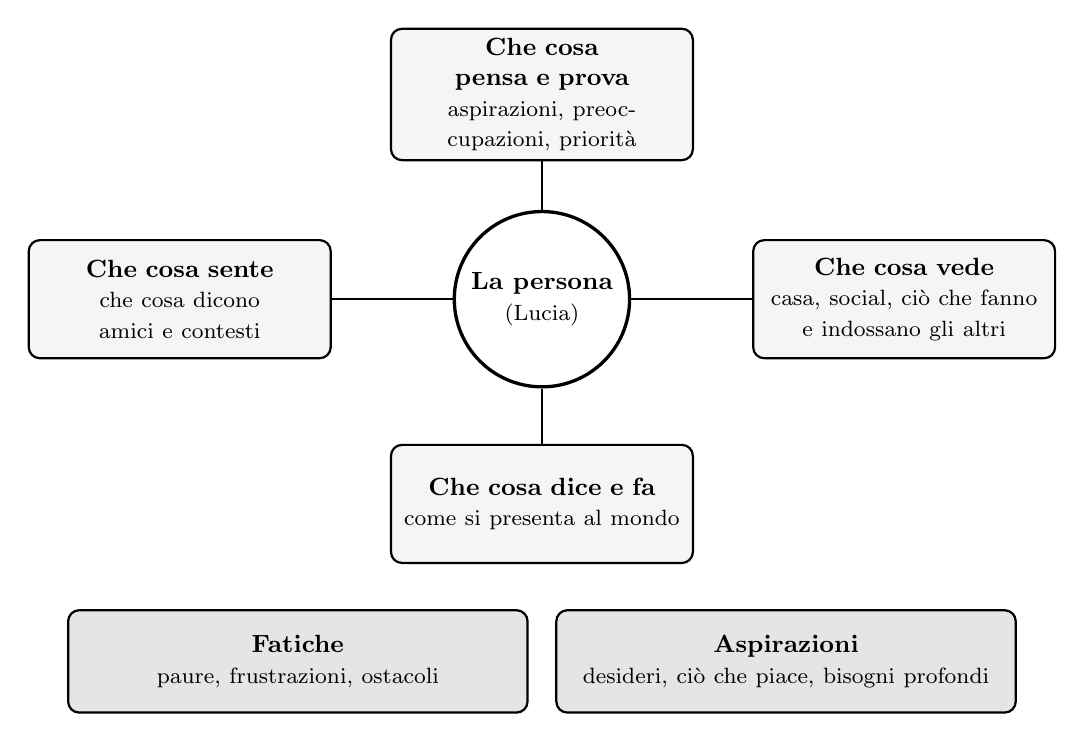
\begin{tikzpicture}[
    font=\small,
    sezione/.style={draw, thick, rounded corners, text width=3.6cm, align=center,
      minimum height=1.5cm, fill=gray!8},
    basso/.style={draw, thick, rounded corners, text width=5.6cm, align=center,
      minimum height=1.3cm, fill=gray!20}
  ]
  \node[draw, very thick, circle, minimum size=2.2cm, align=center, fill=white]
    (p) at (0,0) {\textbf{La persona}\\ \footnotesize (Lucia)};
  \node[sezione] (pensa) at (0,2.6) {\textbf{Che cosa pensa e prova}\\
    \footnotesize aspirazioni, preoccupazioni, priorità};
  \node[sezione] (vede) at (4.6,0) {\textbf{Che cosa vede}\\ \footnotesize casa,
    social, ciò che fanno e indossano gli altri};
  \node[sezione] (sente) at (-4.6,0) {\textbf{Che cosa sente}\\ \footnotesize che
    cosa dicono amici e contesti};
  \node[sezione] (dice) at (0,-2.6) {\textbf{Che cosa dice e fa}\\
    \footnotesize come si presenta al mondo};
  \draw[thick] (p) -- (pensa);
  \draw[thick] (p) -- (vede);
  \draw[thick] (p) -- (sente);
  \draw[thick] (p) -- (dice);
  \node[basso] (fatiche) at (-3.1,-4.6) {\textbf{Fatiche}\\ \footnotesize paure,
    frustrazioni, ostacoli};
  \node[basso] (aspir) at (3.1,-4.6) {\textbf{Aspirazioni}\\ \footnotesize
    desideri, ciò che piace, bisogni profondi};
\end{tikzpicture}
\caption{La mappa dell'empatia come la descrive Beatrice: sei sezioni, con la persona
al centro, e una mappa per ogni tester. Le quattro sezioni superiori si riempiono
chiedendo e osservando; fatiche e aspirazioni sono ciò che se ne ricava.}
\label{a6:fig:empatia}
\end{figure}

\paragraph{Non approfondire è una scelta; non sapere è un errore.} Con i tempi che di
solito si hanno per fare design, non si andrà così nel dettaglio su tutte queste cose
(``oppure sì, dipende''). Ma bisogna sapere che queste informazioni danno tantissimi
strumenti per progettare meglio. \textbf{Decidere di non approfondirle} può essere una
scelta (``non abbiamo il tempo di andare a vedere in che quartiere abita Francesca,
che cosa guarda sui social: dedichiamo più tempo ad altro''); \textbf{non sapere che
sono utili è un errore}.

\paragraph{La mappa come verifica del target.} La mappa serve anche a
\textbf{verificare se il target è quello giusto}. Si parte magari con l'idea di un
gioco che insegni l'inglese, rivolto alle mamme lavoratrici over 40 di una grande
città; e poi si scopre che a loro di un gioco che insegna l'inglese non importa
niente, o che importerebbe se cambiasse la forma del gioco. Questo può far interrogare
sull'obiettivo stesso: forse non è il target giusto, oppure lo è ma bisogna cambiare
qualcos'altro. È un circolo che si raffina pian piano: ``più facciamo design, più ci è
chiaro che direzione dare''.

% ---------------------------------------------------------------------
\section{Come si raccolgono le informazioni}
\label{a6:sec:raccolta}

\slidefig{img/AGD/agd6-fonti}{Fonti social e digitali, e le buone pratiche per intervistare.}{slide \emph{Analog -- Ricerca \& Sviluppo}}{fig:agd6-fonti}


Non sempre c'è il tempo di approfondire così tanto, e non è detto che si ottengano le
risposte che servono: le persone possono non avere tempo, o non avere interesse a
essere sincere, oneste, dirette. La mappa dà le \textbf{direzioni} sulle macro
tematiche; per raccogliere le informazioni si possono fare ``N cose'':
\begin{itemize}
  \item \textbf{domande dirette}, telefonate (Beatrice salta la parte sul
        \textbf{GDPR}, dando per scontato che all'inizio, in questo contesto, si
        lavori con persone che si conoscono; in ambienti più grandi ci sono norme da
        valutare). Dove c'è il tempo, il modo e la situazione per \textbf{parlare a
        voce}, ``top'': è sempre positivo, anche per comunicare il progetto, perché è
        uno scambio in cui si imparano cose sul target e allo stesso tempo ci si fa
        conoscere;
  \item \textbf{internet}, ``un grandissimo dono'': i social network (Reddit,
        Pinterest, Instagram) e gli strumenti per vere e proprie indagini di mercato
        (Google Trends, NotJustAnalytics\footnote{La trascrizione dice ``Google
        Trend, Not Just Analytics''. NotJustAnalytics è uno strumento di analisi dei
        profili Instagram.} e tanti altri);
  \item le domande \textbf{senza comunicazione diretta}: sondaggi, email a cui
        rispondere, e così via\footnote{Beatrice accenna a una slide successiva con un
        libro, ``adesso ci arriviamo''; nella trascrizione il libro non viene poi
        nominato.}.
\end{itemize}
Intervistare le persone resta essenziale. Se lo si riesce a fare già in
pre-progettazione, ``top''; se no, e si fa ricerca in altro modo, sarà comunque
essenziale nel \textbf{playtest}, nell'iterazione e nell'analisi dei feedback, da
osservare direttamente nei primi playtest o da chiedere.

\paragraph{I colleghi.} ``Un'altra cosa che sottovalutiamo molto è chiedere ai
colleghi e alle colleghe''. Qui Gianmarco interviene: nei playtest si consiglia di
\textbf{registrare} come vanno, per vedere che cosa succede? Beatrice vede Ruggero
``che sta vibrando'' e gli passa la domanda. ``La risposta breve è sì, è possibile, ma
con un asterisco su che cosa comporta'': se ne parlerà in modo molto approfondito
nella lezione sul playtest, ``tre ore solo sul playtest''. Ricerca e sviluppo e
playtest hanno parti che si sovrappongono, e qui Beatrice copre ``la parte più a
ombrello'' del processo.

\paragraph{Con le persone bisogna parlarci.} Beatrice riconosce di aver mischiato
le fasi, e spiega perché: le vede spesso sottovalutate, ``e provo proprio rabbia'',
perché ci si appoggia all'idea del \textbf{target come etichetta} (donna di 40 anni,
uomo, giocatore di D\&D), ed è ``sbagliatissimo'': poi non si ha la base per
raccogliere feedback reali, non si capisce più che cosa si sta facendo, e intanto si
lavora su cose che non sono quelle corrette. Del resto la divisione in fasi
(progettazione, playtest, iterazione, uscita) è un'astrazione: durante il playtest,
a seconda del tipo di gioco, possono cambiare cose anche molto grosse; è come se ci
fossero più fasi di \emph{brainstorming}, di playtest, di iterazione, e ogni volta che
cambia anche solo un dettaglio del target o dell'obiettivo bisogna tenerne conto, e la
cosa si ripete. La regola minima, ``insindacabile per un progetto sperimentale in un
corso di sperimentazione'': in tutto il percorso di un gioco bisogna aver fatto
domande e \textbf{ascoltato la voce delle persone}; non per forza filmarle, non per
forza sempre, ma \textbf{almeno due persone dovete sentirle con la voce}. ``Se non lo
fate, c'è un problema''. Poi ci sono anche altri modi, ma una parte delle persone va
sentita dal vivo.

% ---------------------------------------------------------------------
\section{Il target troppo largo: partire da chi si esclude}
\label{a6:sec:nicchia}

\slidefig{img/AGD/agd6-nicchia}{Mercato di massa, segmento e nicchia.}{slide \emph{Analog -- Ricerca \& Sviluppo}}{fig:agd6-nicchia}


Beatrice dà per scontato che a un certo punto ogni gruppo sceglierà un target, e che
in corso d'opera si accorgerà che non è proprio quello corretto; in particolare, che
è \textbf{troppo ampio}. Lo chiama \emph{errore}, ``ma è talmente normale nel
passaggio creativo che non so neanche se chiamarlo errore'': lo chiama così per
ricordare che bisogna starci attenti. Si deciderà di fare una cosa per ``le mamme
quarantenni lavoratrici'', e poi si dirà: no, è troppo grande. \textbf{Non esistono
giochi per tutte le persone}. Anche quando sembra di aver scelto un target con
precisione e con tante caratteristiche, si deve dare per scontato che sia \textbf{una
nicchia troppo grande}: ci si accorgerà che si sta creando un'esperienza per uno
specifico tipo di persone.

La scuola di pensiero di Beatrice: \textbf{se il vostro gioco, e anche la vostra
comunicazione, non esclude qualcuno, state sbagliando qualcosa}. E quindi, se non si
sa da chi partire (perché ``che target scelgo?'' è una domanda gigante),
\textbf{partite almeno da chi non volete}. Se il gioco ha una piccola app, non si può
partire da chi non ha una base di alfabetizzazione digitale; se è un certo tipo di gioco
da tavolo\footnote{La trascrizione dice ``se fate un gioco, un'America''; il tipo di
gioco non è ricostruibile.}, non si può partire da chi non ha mai giocato da tavolo.
Poi si definisce il \textbf{segmento}, e infine la \textbf{nicchia}
(figura~\ref{a6:fig:nicchia}).

\begin{figure}[htbp]
\centering
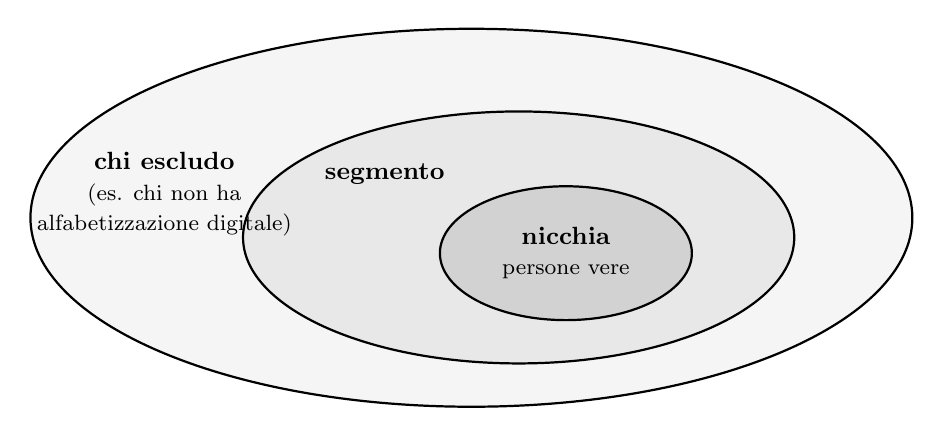
\begin{tikzpicture}[font=\small]
  \draw[thick, fill=gray!8] (0,0) ellipse (5.6cm and 2.4cm);
  \draw[thick, fill=gray!18] (0.6,-0.25) ellipse (3.5cm and 1.6cm);
  \draw[thick, fill=gray!35] (1.2,-0.45) ellipse (1.6cm and 0.85cm);
  \node[align=center] at (-3.9,0.3) {\textbf{chi escludo}\\ \footnotesize (es. chi
    non ha\\ \footnotesize alfabetizzazione digitale)};
  \node[align=center] at (-1.1,0.55) {\textbf{segmento}};
  \node[align=center] at (1.2,-0.45) {\textbf{nicchia}\\ \footnotesize persone
    vere};
\end{tikzpicture}
\caption{Restringere il target: se non si sa da chi partire, si parte da chi si esclude,
poi si definiscono il segmento e la nicchia. ``Non esistono giochi per tutte le
persone''.}
\label{a6:fig:nicchia}
\end{figure}

% ---------------------------------------------------------------------
\section{Le risorse e gli stakeholder}
\label{a6:sec:stakeholder}

\slidefig{img/AGD/agd6-stakeholder}{L'analisi di fattibilità e risorse e l'analisi degli stakeholder.}{slide \emph{Analog -- Ricerca \& Sviluppo}}{fig:agd6-stakeholder}


\paragraph{Le risorse.} Nella lezione successiva si vedrà in dettaglio come decidere
che scelte fare in base alle \textbf{risorse}, che sono di vario tipo: le
\textbf{persone} coinvolte, quindi le competenze; le \textbf{tempistiche}; i
\textbf{soldi}, quando ci sono; i \textbf{materiali}. Se voglio produrre un gioco per
conto mio e investirci i miei soldi, devo valutare quanti e di che tipo: se voglio le
pedine \textbf{in avorio}, il costo sarà diverso che \textbf{in legno}. Queste analisi
vanno fatte sempre \textbf{in parallelo} alla progettazione; spesso sono fatte a monte,
ma per ora l'invito è a farle almeno in parallelo. ``Forse sto andando un po' lunga''.

\paragraph{Gli stakeholder.} ``Ecco, questa slide ci fa abbastanza schifo''; non la
slide in sé, ``frutto del lavoro di persone di qualità'', ma ciò di cui bisogna tenere
conto: ``ci fanno schifo gli \textbf{stakeholder}'', esattamente. Si torna al punto di
prima: se si vuole progettare per i fatti propri, ``top'', e questa slide non
interessa. Se invece si vuole progettare \textbf{tenendo conto dei soldi} (``ve la dico
proprio schietta''), cioè di da dove arrivano i soldi per pagare il lavoro di design,
la \textbf{promozione} (``ahimè, \textbf{un gioco senza promozione non esiste},
ragazzi: questa cosa dobbiamo mettercela via'') e i materiali, le voci sono queste: la
\textbf{creazione}, la \textbf{produzione} con i suoi materiali, la
\textbf{promozione}. Per finanziarle ci sono vari modi già visti: andare da un editore
con un'idea propria, rispondere alla richiesta di un committente. Tutti richiedono di
avere in mente i \textbf{portatori di interesse}, che non sono solo il committente o
l'editore, ma anche i \textbf{potenziali giocatori e giocatrici}, che hanno interesse
a giocare se il gioco è reso di loro interesse. Da un lato ci sono le \textbf{entità
produttive}, dall'altro quelle che \textbf{giocheranno}; tenerne conto in
progettazione è essenziale. In un corso come questo, però, Beatrice non si
soffermerebbe troppo sull'analisi degli stakeholder: basta sapere che, decidendo
\emph{perché} si fa un gioco, si stanno già includendo o escludendo certi stakeholder.
Andare da un editore implica dinamiche diverse dal fare un \textbf{crowdfunding su
Kickstarter}; e voler raccogliere 10.000 euro e non 170.000, facendosi promozione e
``cosine'' per i fatti propri, è un'altra dinamica ancora.

\paragraph{Prepararsi a reagire.} Ruggero chiarisce lo scherzo: non è che gli
stakeholder facciano schifo; è che spesso non è utile tenere tutto in mente. Anche
perché quando ci si interfaccerà con un editore, spesso non si avrà la minima idea di
chi siano gli stakeholder, ``perché neanche l'editore spesso ce l'ha''. Dentro un
publisher ci sono il \textbf{project manager}, lo \textbf{sviluppatore} che lavora sul
gioco, la persona della \textbf{tipografia} che deve tenere bassi i costi: tutte
persone con un interesse nel gioco, che non è detto si conoscano. Il quadro è tanto più
compatto quanto meno il gioco è commerciale (un gioco per sé, che non deve essere
venduto né fatto con nessuno), ma anche lì ci sono persone che sfuggono al controllo.
Quindi: \textbf{non cercate di controllare tutto degli stakeholder}, perché è
impossibile. È una slide ``paradigmatica'', per \textbf{prepararsi a reagire} a ciò che
succede più che per calcolare tutto il possibile, ``perché se no non ne uscite vivi, e
si vede da me in primis''.

\paragraph{Approfondimento: il giocatore come persona, non come categoria.} Schell
dedica un intero capitolo al fatto che il gioco è fatto \emph{per un giocatore},
discutendo demografia (età, genere) e psicografia (che cosa le persone desiderano dal
gioco) e invitando il designer a mettersi nei panni di chi gioca. La lezione spinge
questo invito un passo oltre: le categorie servono a orientarsi ``a volo d'aquila'',
ma il lavoro vero comincia quando la categoria diventa un elenco di persone reali da
ascoltare. È la stessa ragione per cui Schell considera il playtest una fonte di
informazioni insostituibile: ciò che le persone fanno e dicono davanti al gioco
corregge ciò che il designer immaginava di loro.

% ---------------------------------------------------------------------
\section{Gli strumenti e i siti per la ricerca}
\label{a6:sec:strumenti}

\slidefig{img/AGD/agd6-siti}{Canali e strumenti per la ricerca: BoardGameGeek, itch.io, Analog Game Studies, content creator, premi e jam, motori di ricerca.}{slide \emph{Analog -- Ricerca \& Sviluppo}}{fig:agd6-siti}


``Bellissimo: abbiamo un po' di strumenti per fare ricerca e sviluppo, ma \emph{dove}
inizio? Che cosa guardo, dove vado, che cosa leggo?'' Ruggero passa agli
\textbf{strumenti specifici}, o meglio consigliati (tabella~\ref{a6:tab:strumenti}).

\paragraph{BoardGameGeek.} ``Forse il più grosso'': \textbf{BoardGameGeek}\footnote{La
trascrizione dice ``BoardGain Geek'' e ``Boarding Geek''.} è un sito
\textbf{aggregatore} di giochi da tavolo (c'è anche una branca, \textbf{RPGGeek}, sui
giochi di ruolo, meno curata e meno seguita). È gigantesco: se un gioco da tavolo
esiste ed è uscito sul mercato, è in quel database, ed è molto informativo. Dice chi è
l'editore, in quante versioni è stato fatto, chi ha lavorato alle traduzioni, quali
editori l'hanno pubblicato in quali lingue, anni ed edizioni. Rende facile cercare
giochi specifici, divisi per \textbf{tema}, per \textbf{categorie}, per
\textbf{meccaniche}. In homepage c'è la lista della cosiddetta \textbf{Hotness}: una
cinquantina di giochi, i più cercati e con più interazioni sul sito in quel periodo,
aggiornata (se il docente ricorda bene) ogni settimana, con l'indicazione di quali
salgono, quali scendono e quali restano stabili. È una \textbf{fotografia dell'adesso}:
di quali giochi si sta parlando in questo momento nell'ambiente del gioco da tavolo.

\paragraph{itch.io.} Già menzionato da Beatrice e nei casi studio, \textbf{itch.io} è
il luogo per la \textbf{pubblicazione indipendente}: per chi vuole scavalcare un
publisher e pubblicare per conto proprio. È pieno di giochi in \textbf{print and play}
e gratuiti: non si deve andare in stampa, si può vendere anche solo un PDF, spesso con
la formula \textbf{\emph{pay what you want}} (gratis, o un'offerta libera). Si può
cercare per \textbf{tag} (LARP, giochi da tavolo, a pagamento o gratuiti) e scendere
ancora più nel dettaglio sul gameplay. Ed è \textbf{crossmediale}: giochi di ruolo,
giochi da tavolo in print and play, videogiochi, giochi per VR, ``tanta, tanta roba'';
un repository pensato per la pubblicazione indipendente.

\paragraph{Analog Game Studies.} Una ricerca meno sui singoli casi e più su un approccio
\textbf{teorico e accademico}: è il sito citato a proposito del \textbf{Mixing Desk of
Larp}, il cui framework era stato documentato anche a livello di archiviazione storica
proprio lì. Ci sono articoli di \emph{game studies}, di framework, analisi di casi
specifici. È molto variegato e non tutti gli articoli hanno la stessa qualità, ma molti
sono ``davvero molto, molto di qualità'', come quello sul Mixing Desk. Per il docente è
più utile per i \textbf{framework} che per i casi studio, che a volte sono un po'
\emph{mainstream}, pur potendo interessare molte persone.

\paragraph{I content creator.} Database come itch.io e BGG sono bellissimi, ma
``di giochi all'anno ne escono 10.000'': come si capisce che cosa è interessante?
``Purtroppo la soluzione è capire e \textbf{filtrare i content creator} nel tempo''. La
slide ne mette alcuni, misti:
\begin{itemize}
  \item \textbf{Hollandspiele}\footnote{La trascrizione dice ``Holland Spill''.} di
        \textbf{Amabel Holland}, una designer che fa articoli e video sui giochi che fa,
        ma anche molti \textbf{video essay} sulle dinamiche del settore e sul game
        design. Sta anche facendo un lavoro gigantesco di \textbf{archiviazione
        storica}: recuperare chi ha lavorato ai giochi prima che fosse normale mettere
        il nome del designer sulla scatola, cercandolo nei brevetti, nelle
        documentazioni storiche, negli articoli di giornale;
  \item \textbf{Shut Up \& Sit Down} e \textbf{No Pun Included}\footnote{La
        trascrizione dice ``Shadow Pants e Down, Nopane Included''.}, che recensiscono
        i giochi da tavolo in uscita, spesso in anteprima, aggiungendo al ``è bello o
        brutto da giocare'' un layer di \textbf{contesto culturale}: quanto il tema è
        coeso, di che cosa parla il gioco, quanto le meccaniche portano l'emozione o le
        remano contro;
  \item \textbf{Ludology}\footnote{La trascrizione dice ``L'Udology''.}, un podcast di
        game design gigantesco, ``qualitativamente altalenante, con puntate bellissime
        e puntate tremende'', molto sull'approccio al game design dei giochi
        analogici, da tavolo e di ruolo;
  \item \textbf{Cardboard East}, un canale YouTube in inglese che si occupa solo di
        giochi fatti in \textbf{Asia} e nel Sud-est asiatico (Cina, Giappone, Taiwan,
        Corea, Indonesia e così via). Il consiglio è di guardare anche \textbf{altre
        nazioni e culture}: vedere come lo stesso tema è affrontato da un gioco
        occidentale e da uno asiatico è molto interessante;
  \item \textbf{Daniel Solis}, il suo blog e il suo YouTube: non di game design in
        senso stretto, ma di \textbf{pratiche parallele} (graphic design, layout, UX)
        trattate con casi studio di giochi da tavolo.
\end{itemize}
Il tempo è limitato, e la scelta dipende dal \textbf{progetto}: per un gioco di carte
magari Cardboard East non serve, e Daniel Solis sì. È una lista ``microscopica'' e
``molto soggettiva'': creator che piacciono al docente, ``e neanche a tutti''.

\paragraph{Premi e jam.} Le \emph{game jam} erano già state toccate (se ne era parlato all'inizio della lezione precedente); anche i \textbf{premi} servono alla ricerca: capire chi vince
che cosa indica la direzione del mercato.
\begin{itemize}
  \item Lo \textbf{Spiel des Jahres}\footnote{La trascrizione dice ``Speed the Yard''
        e ``Hospital Yard''.} è il premio più famoso del gioco da tavolo. Si può non
        essere d'accordo con i giochi che premia (``in molti non lo siete, io
        incluso''), e ci sono anche questioni sociali ``perniciose'' che il docente
        non apre; ma i giochi premiati vendono moltissimo, e capire quali vengono
        premiati dice che cosa il \textbf{mercato europeo} vuole vedere sul tavolo, il
        che informa i negozianti, gli editori, e così a catena.
  \item Eventi più piccoli, che non hanno premi ma danno un \textbf{tempo limitato} per
        creare un gioco: la ``Pub Jam'' per i giochi da tavolo, la \textbf{Golden Cobra
        Challenge} per i LARP, e un contest per giochi di ruolo da tavolo e LARP che
        la trascrizione chiama ``Freak Form'' e ``Flickform''\footnote{Né la ``Pub
        Jam'' né ``Freak Form''/``Flickform'' sono ricostruibili con sicurezza dalla
        trascrizione; il capitolo riporta le forme registrate.}.
  \item Premi più indipendenti, ``non meno importanti'': lo \textbf{Zenobia Award},
        per giochi da tavolo di persone che vengono da minoranze o da comunità che
        non hanno avuto grande spazio nel gioco da tavolo, e il \textbf{Diana Jones
        Award}, che premia l'eccellenza soprattutto nel gioco di ruolo da tavolo.
        Seguire chi vince, che cosa pubblica, quali editori lo seguono, è utile se si
        vuole andare in quella direzione.
\end{itemize}

\paragraph{I motori di ricerca.} Infine, ``so che sembra banale, ma non è scontato'':
\textbf{cercate}. ``Vi sorprenderà sapere quante persone stanno facendo un gioco su un
tema e non hanno cercato neanche su Google quali giochi su quel tema sono usciti''.
Non per bloccarsi (``l'hanno già fatto, a posto, non lo faccio più''), ma per sapere
che cosa hanno fatto gli altri: in che cosa è simile a ciò che si vuole offrire, in che
cosa è diverso. Sullo stesso tema si possono avere \emph{take} completamente diversi.
L'esempio, ``stupido, ma per capirci'': i \textbf{giochi di guida}. C'è il simulativo
(\emph{Gran Turismo}), l'arcade (\emph{OutRun}), il party ``molto caciarone''
(\emph{Super Mario Kart}): tutti giochi di guida, con take diversissimi. ``Non vorrei
che pensaste: voglio fare \emph{Gran Turismo}, però esiste già \emph{Super Mario Kart},
allora non lo faccio''. \textbf{Non fatevi limitare dai giochi che esistono}: copiate,
trasformate, combinate; fate diverso ciò che non vi piace, simile ciò che vi piace, e
\textbf{ditelo}.

\begin{table}[htbp]
\centering
\small
\begin{tabular}{@{}p{3.2cm}p{3.0cm}p{6.8cm}@{}}
\toprule
\textbf{Strumento} & \textbf{Tipo} & \textbf{A che cosa serve} \\
\midrule
BoardGameGeek (e RPGGeek) & database aggregatore & ogni gioco da tavolo uscito:
editori, edizioni, lingue, temi, categorie, meccaniche; la Hotness come fotografia
del momento \\
itch.io & piattaforma indipendente & print and play, PDF, \emph{pay what you want};
ricerca per tag; crossmediale (anche videogiochi e VR) \\
Analog Game Studies & sito accademico & articoli teorici, framework (il Mixing Desk),
casi studio di qualità variabile \\
Hollandspiele (Amabel Holland) & designer, video essay & dinamiche del settore,
archiviazione storica dei designer non accreditati \\
Shut Up \& Sit Down, No Pun Included & recensioni & giochi in uscita con contesto
culturale: coesione del tema, meccaniche ed emozione \\
Ludology & podcast & game design dei giochi analogici; qualità altalenante \\
Cardboard East & canale YouTube & giochi dell'Asia e del Sud-est asiatico; confronto
tra culture \\
Daniel Solis & blog e YouTube & graphic design, layout e UX applicati ai giochi da
tavolo \\
Spiel des Jahres & premio & che cosa vuole il mercato europeo; i premiati vendono
moltissimo \\
Golden Cobra e altre jam & contest a tempo & creare in tempo limitato (LARP, giochi da
tavolo, giochi di ruolo) \\
Zenobia Award, Diana Jones Award & premi indipendenti & minoranze nel gioco da
tavolo; eccellenza nel gioco di ruolo \\
Motori di ricerca & --- & sapere che cosa esiste sul tema, per differenziarsi e non
per rinunciare \\
\bottomrule
\end{tabular}
\caption{Gli strumenti per la ricerca consigliati da Ruggero. ``Una lista microscopica
e molto soggettiva'': da filtrare in base al progetto.}
\label{a6:tab:strumenti}
\end{table}

\paragraph{Progettate il vostro percorso.} ``Questo è tutto per quanto riguarda le
slide''. È stata tanta roba, e altra arriverà in asincrono con la dispensa di Daniele.
Non c'è l'obbligo di usare tutti questi strumenti: i lavori di gruppo saranno in
autogestione. ``Però vogliamo vedere che \textbf{qualcosa usate}'', che non si vada
alla cieca, ma che idealmente, come ha detto Beatrice (e come si vedrà in due lezioni
con lei), \textbf{ci si progetti il percorso}. Anche perché così si butta via meno
tempo: se si sa che per una cosa ci vuole tanto tempo e per un'altra tanto, non si
finisce col dire ``mi aspettavo un gioco da fare in tre ore e sono due mesi che scrivo
il regolamento''. (Il docente chiude con una battuta un po' nera che richiama il gioco
di Angelo e la raccomandazione sui content warning.)

% ---------------------------------------------------------------------
\section{Le domande finali}
\label{a6:sec:domande}

``Che silenzi. Qualcuno ha domande?''

\subsection{Esiste un catalogo di meccaniche ed emozioni?}
\label{a6:sec:catalogo}

Tiziana chiede conferma di una cosa che forse le è già stata detta: dopo l'esercizio
del task, esiste qualcosa da leggere che, a partire da ciò che è già stato fatto,
spieghi la \textbf{relazione tra meccaniche ed emozioni}, o esperienze?

\paragraph{Non esiste una fonte singola.} ``Vorrei dirti di sì, ma non esiste''.
Esistono tanti frammenti, di persone con opinioni molto diverse, a volte contrastanti,
``a volte anche che litigano di brutto tra di loro''. Per capire quanto è profonda ``la
tana del Bianconiglio'': nell'ambito accademico c'è stata una diatriba durata una
dozzina d'anni, e in alcune nicchie ancora viva, tra \textbf{ludologi} e
\textbf{narratologi}. I narratologi sostenevano che il gioco comunica attraverso i suoi
aspetti narrativi: se un gioco ha emozioni e un tema, sono gli aspetti narrativi a
darli. I ludologi rispondevano che il gioco comunica con le \textbf{meccaniche}, non
con la narrazione, e che un gioco che si basa sulla narrazione e non solo sulle
meccaniche è un gioco fallimentare. Entrambi i gruppi, per il docente, sono
``completamente sregolati nel loro estremismo''; ma la faida fa capire quanto siano
diversi i punti di vista su che cosa un gioco debba avere. Il docente non dirà di non
mettere narrazione, o di mettere solo narrazione: vuole dare più strumenti possibili
per portare chi gioca in un'\textbf{area emotiva}. E quella cosa, ``purtroppo o per
fortuna'', \textbf{si fa di solito con le meccaniche}; ci sono tante cose che danno una
mano (si vedranno nel paragame), ``ma stiamo facendo giochi e non libri'', e la
priorità va alle meccaniche.

\paragraph{I cataloghi esistenti, e il loro limite.} Che cosa portano le meccaniche
``è un bel casino''. Alcuni ambiti del gioco analogico hanno dedicato più spazio a
questa domanda: \emph{Building Blocks of Tabletop Game Design} di Geoffrey Engelstein
(e Isaac Shalev)\footnote{La trascrizione dice ``Building Blocks of Board Game Design,
quello di Geofengelstein'' e ``il libro di Valternuccio''.}, ``la versione inglese,
se vogliamo'', del libro di \textbf{Walter Nuccio}, un database di meccaniche che prova
a spiegare per ciascuna, più o meno, dove porta emotivamente. Ma è molto
\textbf{atomizzato}: non dice che cosa succede quando si mettono insieme tre o quattro
meccaniche diverse, e bisogna intuirlo. Solo nel gioco da tavolo le meccaniche sono
tantissime (\emph{drafting}, \emph{worker placement}, aste aperte e chiuse,
\emph{take that}, controllo d'area, \emph{set collection}\ldots): che cosa succede
quando le si mischia? E due giochi che sulla carta hanno le stesse meccaniche
possono dare al tavolo esperienze completamente diverse, ``e questo spero che lo
sappiate già''.

\paragraph{La frustrazione e i layer meta.} Tiziana capisce: si individua un'area, e ci
si concentra più sull'esperienza che sull'emozione specifica. La sua era una curiosità:
per esperienza, la cosa macro che può dire di un gioco da tavolo è se prova
\textbf{frustrazione} o no, in base a quanto riesce a gestire il gioco. Certo, risponde
il docente, ma ci sono dei \textbf{layer meta}: si può provare frustrazione non perché
il gioco voglia farla provare, ma perché ``il regolamento è scritto male'', e allora
non sono le meccaniche, è il regolamento a portarla. E c'è un \textbf{layer di
interpretazione} di che cosa il gioco voglia dire. Il gioco di Angelo: un gruppo lo
legge come un gioco che comunica \textbf{disperazione} e lo gioca su quell'emozione;
un altro lo legge come un gioco di \textbf{speranza} (``posso salvare anche la persona
che è sull'orlo''), e quella partita sarà emotivamente diversa. È sempre un lavoro di
\textbf{compromesso}: la difficoltà di chi fa game design è capire come
\textbf{ridurre quell'area il più possibile}, per renderla meno ambigua. Non è una cosa
che si ragiona in astratto: è esperienza ``con le mani in pasta''.

\paragraph{Nessuno lo sa leggendo.} ``Ve lo dico e ve lo giuro: di giochi ne avrò fatti
più di cinquanta, e tuttora non conosco una singola persona, me incluso, che dalla
lettura di un regolamento sappia dire esattamente che cosa quel gioco porta
emotivamente, senza vederlo giocato o senza giocarlo''. Se fosse così facile,
\textbf{non esisterebbero i playtest}. ``Purtroppo, o per fortuna'': farlo è
\textbf{fare i giochi}, testarli, vederli giocare, giocarli. La parola chiave è
\textbf{euristiche}: l'esperienza pregressa che informa come si vivono le esperienze
successive. Dopo tre o quattro giochi di un certo tipo, ``un po' di cose le ho
imparate: questo genere di giochi so farlo un po' meglio''.

\paragraph{Il contesto cambia (Beatrice).} Beatrice aggiunge: la cosa importante è
fare \textbf{tanta ricerca e tanta sperimentazione}, perché è così che si capiscono e
si vedono le cose; per questo il corso dedica tanto spazio alla ricerca e sviluppo, e il
playtest sarà fondamentale per ascoltare i feedback. Ma la \textbf{certezza} non ci
sarà mai, perché non si conosce il contesto in cui tutte le persone sono inserite: per
questo contano la mappa dell'empatia e l'idea di target. Se un gioco fatto oggi lo si
gioca tra vent'anni, il contesto è già cambiato: \emph{Casablanca} visto adesso e visto
quando è uscito dà effetti emotivi molto diversi, come qualunque film o gioco vecchio.
Non si può avere piena consapevolezza di tutte le persone che giocheranno, in che
contesto saranno, che cosa saranno; si può lavorare sul \textbf{qui e ora}, ``che è
anche un grande esercizio di vita'', e informarsi il più possibile. Non esistono giochi
per tutti, e nessuna persona risponde esattamente a un'etichetta: ``è un po' un
balletto''. Il consiglio: puntare meno sul \emph{come ottengo esattamente quello che
voglio} e più sul \textbf{come ascolto bene i feedback} che ricevo, e ragionare su
quelli. ``È un cambio di paradigma importante'': sembra di rinunciare a un po' di
controllo, ``ma non è vero''.

\paragraph{Il divario tra chi fa e chi gioca.} Tiziana precisa che non cercava il
controllo: già facendo l'esercizio aveva capito che non è possibile. Basta mettere
ruoli diversi, come il medico e il paziente del suo gioco, perché le emozioni siano
completamente diverse; per i suoi compagni di gioco erano in alcuni casi
diametralmente opposte. Qual è allora l'emozione dominante? Dipende dal personaggio.
Il docente (con ogni probabilità Ruggero) le dice che il tema gli interessa
particolarmente: la sua \textbf{tesi di master in design} era proprio sul \textbf{gap
di interpretazione} tra l'emozione intesa da chi fa il gioco e quella di chi lo gioca,
intervistando separatamente le due parti (``tu, designer, che cosa volevi fare? Tu che
hai giocato, che cosa secondo te il gioco comunicava?''). \textbf{È impossibile colmare
quel gap del tutto}: lo si può solo \textbf{ridurre}, ``perché nessuno è voi, solo voi
siete voi''. E molte cose sfuggono al controllo anche sul piano produttivo: si vuole
stampare il gioco in un modo e non si può, o costa troppo, e i compromessi sono tagliati
a monte. In più, come si vedrà nella parte su prototipazione e regolamento,
\textbf{il regolamento è un medium lineare, ma i giochi sono ecosistemi}: una regola ne
impatta un'altra, che impatta la precedente. Come le si mette in formato lineare? ``Lo
vedremo più avanti''.

Beatrice chiude il punto sottolineando che nessuno aveva colto in Tiziana una voglia di
controllo: il discorso voleva solo dire che la classe ha fatto un grande lavoro sulle
emozioni, e che poteva passare il sottotesto ``avete pensato che arrivate a B, e
arrivate sicuramente a B''. ``Invece non è proprio così: è più sfumato''.

\begin{figure}[htbp]
\centering
\begin{tikzpicture}[
    font=\small,
    blocco/.style={draw, thick, rounded corners, minimum height=1.2cm,
      text width=2.8cm, align=center},
    freccia/.style={-{Stealth[length=2.5mm]}, thick}
  ]
  \node[blocco, fill=gray!10] (d) at (0,0) {\textbf{Emozione intesa}\\
    \footnotesize da chi progetta};
  \node[blocco, fill=gray!20] (r) at (4.6,0) {\textbf{Regolamento}\\ \footnotesize
    lineare, ma il gioco è un ecosistema};
  \node[blocco, fill=gray!30] (g) at (9.2,0) {\textbf{Emozione vissuta}\\
    \footnotesize da chi gioca};
  \draw[freccia] (d) -- (r);
  \draw[freccia] (r) -- (g);
  \node[font=\footnotesize, align=center, text width=3.4cm] at (2.3,-1.4)
    {compromessi produttivi; layer meta (regole scritte male)};
  \node[font=\footnotesize, align=center, text width=3.4cm] at (6.9,-1.4)
    {interpretazione; ruoli diversi; contesto e tempo};
  \draw[{Stealth[length=2mm]}-{Stealth[length=2mm]}, dashed] (d.north) to[bend
    left=25] node[above, font=\footnotesize] {il gap: si può ridurre (meccaniche,
    playtest, euristiche), non colmare} (g.north);
\end{tikzpicture}
\caption{Il divario tra l'emozione intesa e l'emozione vissuta, come emerge dalle
domande finali. Lo si restringe con le meccaniche, il playtest e l'esperienza
accumulata; non lo si elimina.}
\label{a6:fig:gap}
\end{figure}

\subsection{Le escape room}
\label{a6:sec:escape}

Beatrice usa gli ultimi minuti per una domanda ``che può sembrare un po' strana'': a
quante persone del gruppo interessano le \textbf{escape room} come progettazione?
Rispondono una studentessa\footnote{La trascrizione dice ``Cristiana'', nome che non
corrisponde a nessuno degli iscritti; potrebbe trattarsi di Tiziana.} e Lorenzo
(``sì, sono interessato''). ``Mi è già sufficiente''. Il motivo: per le lezioni
successive i docenti hanno preparato una sorta di \textbf{percorso guidato}, uno schema
di come si può progettare un gioco con i tempi e la struttura del corso, per allenarsi
ad avere una direzione. Beatrice vorrebbe inserirci anche un \textbf{modulo sulle
escape room}, già previsto, ma a cui si è dato meno spazio per scelte fatte in corso
d'opera, ``perché adattiamo molto il corso alle persone che partecipano''. Ci dormirà
su, si confronterà con i colleghi, e il tema sarà comunque toccato; si capirà insieme
quanto approfondirlo.

\subsection{I saluti}
\label{a6:sec:saluti}

C'è tempo per un'ultima domanda. Uno studente ringrazia: tra dieci minuti deve uscire
di casa, ``ci vediamo lunedì''. Un'altra chiede se i docenti manderanno delle domande a
cui rispondere. No: Daniele manderà una \textbf{dispensa}, ``non credo oggi, nei
prossimi giorni'', e comunque \textbf{non è per lunedì}. Non sono domande, è
\textbf{materiale aggiuntivo}: uno \emph{zoom} più dettagliato sugli strumenti di
\emph{brainstorming} che per motivi di tempo non sono entrati nella lezione, ``che era
già bella piena''. Non è obbligatorio e non ci saranno interrogazioni sugli strumenti;
come sempre, sono strumenti in più per lavorare. Li si trova nel Drive, nella
cartella delle dispense. Beatrice saluta e augura buon weekend; Ruggero ricorda che
lunedì la lezione è con lei. ``Ciao ciao, buon weekend''.

% ---------------------------------------------------------------------
\section*{Punti chiave del capitolo}
\addcontentsline{toc}{section}{Punti chiave del capitolo}

\begin{itemize}
  \item Non si controlla l'esperienza di chi gioca: si definisce un'\textbf{area
        emotiva} e la si restringe con le meccaniche e il playtest. Nel 200 Word RPG
        ci sono componenti comuni (un mazzo standard sì, un mazzo di prompt no) e
        niente colpi di scena: ``con le cose che ho in casa adesso posso partire a
        giocare?''. Nel task conta il \textbf{processo}, non l'idea migliore: le idee
        sono tante, conta l'\textbf{esecuzione}.
  \item Il \textbf{metodo di lettura}: il regolamento letto ad alta voce come da chi
        l'ha appena scaricato, l'autore che tace e si segna le ambiguità, poi le
        emozioni secondo la classe e secondo chi l'ha scritto.
  \item Dai nove giochi: regole implicite sì, se non lasciano scelte aperte; dichiarare
        il \textbf{player count}; attenzione alle meccaniche che tolgono
        \textbf{agency} (il gioco dell'oca); il \textbf{buon senso} non è una regola,
        e ``fate come volete'' non è design; l'emozione \textbf{non si scrive} (né
        nominando un valore né descrivendo come ci si sentirà); i temi delicati
        chiedono \textbf{content warning}, meccaniche di sicurezza e consulenti; i
        freeform aperti rischiano di far sfuggire tema e messaggio;
        \textbf{terminologia} costante, niente riferimenti culturali locali, nessun
        cambio di genere non annunciato; \textbf{un regolamento non è un pitch}.
  \item Si fa ricerca per conoscere lo \textbf{stato dell'arte}, prendere decisioni,
        posizionarsi, validare idee, rispondere a domande, tenere la mente elastica e
        \textbf{comunicare l'innovazione}. È costante (``come la botanica'') e legata
        al progetto. Per ogni fase un motore: ispirazione (anche fuori dai giochi),
        cristallizzare la visione (la notte da soli nel bosco), mix e remix,
        validazione e mercato.
  \item \textbf{Divergenza} (il calderone delle idee) e \textbf{convergenza}
        (selezione in base agli obiettivi), ripetute nel doppio diamante: avere tante
        idee è normale. Gli strumenti della dispensa di Daniele non vanno imparati
        tutti: si prendono quelli che risuonano.
  \item La creatività non è mistica: è \textbf{copiare, trasformare, combinare}
        (\emph{Age of Steam} e \emph{Steam}; \emph{Magic} e \emph{Dominion};
        \emph{Scrabble} più \emph{Dominion} uguale \emph{Paperback}), anche
        crossmediale. Siatene consapevoli. Le meccaniche non sono tutelabili, nomi,
        loghi e aspetto sì (il caso \emph{Bang!} e \emph{Samurai Sword}); niente
        proprietà intellettuali altrui; \textbf{dichiarate le ispirazioni}.
  \item Gli step per validare un'idea: \textbf{obiettivo personale} (perché faccio
        design adesso?), \textbf{obiettivo del gioco} condiviso dal team (i pinguini
        blu), \textbf{ipotesi}, \textbf{prototipo}, \textbf{validazione} con il
        playtest; e poi di nuovo. È una linea guida: ``ci sarà un gran casino''.
  \item Il \textbf{target} viene prima di meccaniche e grafiche, e non è solo
        marketing: bambini di 7 anni e banchieri in pausa pranzo sono giochi diversi.
        Ma il target non è un'etichetta: è una \textbf{lista di persone vere}, con nome
        e contatti. La \textbf{mappa dell'empatia} (sente, pensa e prova, vede, dice e
        fa; fatiche e aspirazioni) va fatta per ogni tester, e serve anche a
        verificare il target. Non approfondire è una scelta, non sapere è un errore.
  \item Le informazioni si raccolgono a voce (il meglio), online (social, Google
        Trends), con sondaggi; si chiede ai colleghi. Regola minima: \textbf{almeno due
        persone sentite con la voce}. Il target sarà sempre troppo largo: non esistono
        giochi per tutti; \textbf{se il gioco non esclude qualcuno, c'è qualcosa che
        non va}; si parte da chi si esclude, poi segmento e nicchia.
  \item Le \textbf{risorse} (persone, tempi, soldi, materiali: avorio o legno) si
        valutano in parallelo al design. Gli \textbf{stakeholder} vanno dall'editore
        ai giocatori; ``un gioco senza promozione non esiste''; non si controllano
        tutti: ci si prepara a reagire.
  \item Gli strumenti: \textbf{BoardGameGeek} (e la Hotness), \textbf{itch.io},
        \textbf{Analog Game Studies}, i content creator (Amabel Holland, Shut Up \&
        Sit Down, No Pun Included, Ludology, Cardboard East, Daniel Solis), i premi
        (Spiel des Jahres, Zenobia, Diana Jones) e le jam (Golden Cobra), e i motori di
        ricerca: per differenziarsi, non per rinunciare (\emph{Gran Turismo},
        \emph{OutRun}, \emph{Mario Kart}).
  \item Non esiste un catalogo unico di \textbf{meccaniche ed emozioni}: c'è la faida
        tra ludologi e narratologi, ci sono cataloghi atomizzati (Engelstein, Nuccio),
        ci sono layer meta e di interpretazione. Nessuno sa che cosa farà provare un
        gioco leggendone il regolamento: per questo esiste il playtest, e contano le
        \textbf{euristiche}. Il gap tra emozione intesa e vissuta si riduce, non si
        colma; il contesto cambia nel tempo (\emph{Casablanca}); meglio puntare
        sull'\textbf{ascolto dei feedback} che sul controllo. Il regolamento è lineare,
        il gioco è un ecosistema.
\end{itemize}

%    % =====================================================================
%  Analog Game Design, lezione 7 — Obiettivi di design e design sprint:
%  l'annuncio dei gruppi e del project work (mandate, calendario, pitch
%  del 12 ottobre, regole di lavoro sul Drive); perché si fa game design
%  (obiettivo del gioco e obiettivo personale: pubblicare, esprimersi,
%  formare e sensibilizzare, fare marketing, e le competenze che ognuno
%  richiede); un esercizio di design sprint fatto da tutta la classe su
%  una lavagna di Canva (la chiacchierata iniziale, l'obiettivo del
%  gioco, il racconto delle idee, la votazione a pallini, la ricerca e
%  sviluppo, la mappa impatto-sforzo, il percorso dell'utente, "state
%  sul semplice"); in coda, il primo tutoraggio con Ruggero (emozioni
%  prima delle meccaniche, il gioco del traditore, Tabletop Simulator,
%  che cos'è il pitch, il Mixing Desk come paletti e non come
%  validazione).
%  Fonte: trascrizione della settima lezione (AGD7) del corso breve di
%  Analog Game Design, seconda edizione: una lezione online di circa
%  tre ore (apertura di Daniele, poi Beatrice), con una pausa breve
%  alle 19:10, seguita nello stesso file dalla registrazione del primo
%  tutoraggio di gruppo, un'ora su Meet con Ruggero, tre giorni dopo.
%  Pacchetti richiesti nel preambolo del libro (già presenti nel
%  main.tex): \usepackage{booktabs}, \usepackage{tikz} con
%    \usetikzlibrary{shapes.geometric,shapes.symbols,shapes.misc,
%      arrows.meta,positioning,calc,fit}
%  (le librerie vanno caricate nel preambolo, non nel capitolo).
%  Consigliati, come per gli altri capitoli: \usepackage[italian]{babel}
%  e \usepackage[T1]{fontenc} (il capitolo compila anche senza).
%
%  Collocazione nel libro: parte "Analog Game Design", settimo capitolo
%  (numerazione propria 2.7). Nel file principale del libro, subito dopo
%  il capitolo 2.6:
%
%    \input{AGD/AGD6_ricerca_e_sviluppo}
%    \input{AGD/AGD7_obiettivi_e_design_sprint}
%
%  Tutte le etichette di questo capitolo hanno il prefisso "a7:"
%  (a7:cap:..., a7:sec:..., a7:fig:..., a7:tab:...). Il capitolo è
%  autonomo: non contiene \ref verso altri capitoli.
%  Le figure e le tabelle sono ricostruzioni schematiche di quanto i
%  docenti spiegano a voce, con le slide e sulla lavagna condivisa, non
%  copie delle slide. Le idee degli studenti sono riassunte come le
%  raccontano loro, ripulite dagli errori del riconoscimento vocale;
%  dove la trascrizione è troppo rovinata per ricostruire un dettaglio,
%  il capitolo lo dice invece di inventarlo.
% =====================================================================

\chapter[Obiettivi di design e design sprint]{Obiettivi di design e design
sprint: i gruppi, il perché di un gioco e un primo gioco inventato insieme}
\label{a7:cap:sprint}

Questa è la \textbf{settima lezione} del corso di \textbf{Analog Game Design}, ed è
la lezione in cui il corso cambia passo. Fino a qui gli studenti hanno lavorato da
soli, sui task ``didattici'' (il personaggio, il gioco di ruolo in 200 parole); da
oggi lavoreranno \textbf{in gruppo} sul \textbf{project work}, il gioco analogico
che accompagnerà tutto il resto del corso. La lezione si apre quindi con Daniele,
che annuncia i \textbf{gruppi}, il \emph{mandate} (che cosa si deve fare e che cosa
no), il \textbf{calendario} e le regole pratiche per lavorare. Poi la parola passa a
Beatrice, che fa due cose. La prima è un ``cappellino introduttivo'' su
\textbf{perché si fa game design}: un gioco ha un obiettivo suo, ma anche chi lo fa
ha un \textbf{obiettivo personale} (pubblicare, esprimersi, formare, fare
marketing), e ognuno di questi obiettivi chiede competenze diverse. La seconda, che
occupa la maggior parte del tempo, è un \textbf{esercizio di design sprint}: tutta
la classe finge di essere un unico gruppo di nove persone e, su una lavagna
condivisa, percorre le fasi che porterebbero da zero al \emph{pitch} di un gioco.
L'esercizio produce un vincitore inatteso (``i funghi hanno un sacco di successo,
non me lo immaginavo'') e, soprattutto, un metodo da riusare quando un gruppo si
blocca: timer, post-it, votazione a pallini, ricerca, \textbf{mappa impatto-sforzo},
\textbf{percorso dell'utente}, e la regola d'oro ``\textbf{state sul semplice}''.

La trascrizione contiene anche, in coda, la registrazione del \textbf{primo
tutoraggio}, che il capitolo riporta per intero perché ne è la naturale
prosecuzione: un'ora con \textbf{Ruggero}, tre giorni dopo, ``guidata dalle vostre
domande''. Lì tornano i temi della lezione, visti dall'interno dei gruppi appena
nati: perché partire dalle \textbf{emozioni} e non dalle meccaniche, che cosa ci si
aspetta davvero dal \textbf{pitch} del 12 ottobre, come usare il \textbf{Mixing
Desk} senza farsene schiacciare, e come prepararsi alla lezione su
\textbf{Tabletop Simulator} del giorno dopo.

La lezione è \textbf{online} e ha tre voci. Apre \textbf{Daniele}\footnote{Come
nelle lezioni precedenti, il cognome non è ricostruibile con certezza: qui la
trascrizione lo fa pronunciare a Daniele stesso come ``Daniele Fusetto'' (nella
prima lezione era ``Daniel Cusetto'').}, che resta solo ``per la presentazione dei
gruppi'' e poi si scollega per un'altra riunione; prosegue \textbf{Beatrice}
(``Bea''), che conduce tutta la lezione e l'esercizio; \textbf{Ruggero} non c'è
alla lezione (è nominato più volte, anche come ``Ruger'' e ``Rugger'') ma conduce
il tutoraggio. La lezione si colloca con ogni probabilità \textbf{lunedì 28
settembre 2026}\footnote{La data non è detta, ma è ricostruibile: Daniele parla
della lezione di ``venerdì'' (quella sulla ricerca e sviluppo, del 25 settembre)
come appena passata, ricorda che Gianmarco ``come sempre, lunedì'' arriva verso le
sei, e annuncia il tutoraggio per ``giovedì 1 ottobre''. Nel tutoraggio uno
studente parla della ``lezione di lunedì'' sui funghi e Ruggero osserva ``siamo a
ottobre''.}, dalle 17 alle 20 circa: la pausa è dalle \textbf{19:10} alle
\textbf{19:15}, e la sessione di ricerca finisce alle \textbf{19:32}. Il tutoraggio
è \textbf{giovedì 1 ottobre}, alle 17, su Meet, e dura un'ora. In classe ci sono
\textbf{Tiziana}, \textbf{Rita}, \textbf{Tancredi}, \textbf{Giordano},
\textbf{Angelo}, \textbf{Gianmarco} (che arriva a esercizio iniziato),
\textbf{Nicola} (che arriva ancora più tardi) e i \textbf{due Lorenzo}: Lorenzo
Vergata e l'altro Lorenzo, che durante la lezione propone di farsi chiamare con il
secondo nome, ``John'', per evitare confusioni\footnote{``Non ce la posso fare, i
doppi nomi mi devastano'', dice Beatrice. L'altro Lorenzo spiega che il suo secondo
nome è John, ``non sto scherzando'', e Beatrice se lo appunta come ``Lorenzo L.''.
Nel capitolo lo si chiama ``l'altro Lorenzo''; Lorenzo Vergata è chiamato per nome e
cognome quando serve distinguerli.}.

Tre avvertenze di lettura, le stesse dei capitoli precedenti. La prima: la
trascrizione è automatica e storpia moltissimi nomi. Angelo diventa spesso
``Angela'' (e una volta ``Angevo''), Tiziana ``Tiziano'' e ``Cristiana'', Bea
``Bianca'', Tancredi ``Tankerat'' e ``Tank'', Canva ``Kamba'' e ``gamba'', Tabletop
Simulator ``Temuto Simulator'', ``Table of Simulator'' e ``Debox Monitor''; i giochi
citati non vanno meglio (\emph{Hanabi} è ``Anabis'', \emph{Mage Knight} ``Image
Night'', \emph{Harmonies} ``Armonies''). Dove la ricostruzione è sicura, o molto
probabile, il capitolo usa la forma corretta e lo segnala in nota la prima volta;
dove non lo è, riporta la forma della trascrizione e lo dice. La seconda: nei
momenti in cui la classe lavora in silenzio sotto timer (mentre si scrivono i
post-it, durante la votazione, nella pausa e nei dieci minuti di ricerca) la
trascrizione registra per decine di righe frasi senza alcun rapporto con la lezione,
ripetute in loop (``la situazione è questa, la migliore dal 2005'', ``il numero di
persone è molto più basso'', ``qual è la risposta che ci può essere?'', discorsi
su governi, parlamenti e ``dottrine sul mercato del lavoro''); anche l'apertura
contiene alcune frasi di questo tipo, e a un certo punto un ``scusi'' ripetuto
trenta volte. Sono artefatti del riconoscimento vocale e il capitolo le ignora. La
terza: gli studenti intervengono spesso senza che la trascrizione segnali chi
parla; il capitolo li nomina quando il contesto lo rende chiaro e resta generico
altrimenti.

\paragraph{Come leggere questo capitolo.} La lezione è in gran parte un
\textbf{laboratorio}: conta meno \emph{che cosa} è uscito dall'esercizio (un gioco
sui funghi che nessuno svilupperà) e più \emph{come} ci si è arrivati, e che cosa è
andato storto lungo la strada (i tempi sforati, i commenti che si infilano tra le
domande, le idee troppo personali). Beatrice lo dice più volte: ``lo strumento ci
interessa il giusto'', ``ci interessa il procedimento''. Il capitolo segue quindi
la lezione passo per passo, riportando le idee di tutti, e segnala ogni volta la
regola di metodo che il passaggio illustra. Qua e là, dei paragrafi di
\textbf{approfondimento} collegano la lezione ai libri di game design di riferimento
(soprattutto \emph{The Art of Game Design} di Jesse Schell) e alla letteratura sul
design sprint; sono segnalati come tali e non fanno parte della lezione.

Il percorso del capitolo segue quello della lezione:
\begin{enumerate}
  \item l'attesa (sezione~\ref{a7:sec:attesa});
  \item il \textbf{project work}: calendario, \emph{mandate}, gruppi, regole di
        lavoro (sezioni da~\ref{a7:sec:calendario} a~\ref{a7:sec:regole});
  \item \textbf{perché facciamo game design}: obiettivo del gioco e obiettivo
        personale, e le competenze che ogni obiettivo richiede (sezioni
        \ref{a7:sec:obiettivi} e~\ref{a7:sec:competenze});
  \item il \textbf{design sprint}: che cos'è, il file con le fasi, la
        chiacchierata iniziale, la lavagna di Canva (sezioni
        da~\ref{a7:sec:sprint} a~\ref{a7:sec:canva});
  \item l'esercizio: l'\textbf{obiettivo del gioco}, il racconto delle idee di
        tutti, la \textbf{votazione a pallini} (sezioni da~\ref{a7:sec:fase1}
        a~\ref{a7:sec:votazione});
  \item dopo la pausa: i tempi, la \textbf{ricerca e sviluppo}, le fasi
        successive, la \textbf{mappa impatto-sforzo}, il \textbf{percorso
        dell'utente} e ``state sul semplice'' (sezioni da~\ref{a7:sec:tempi}
        a~\ref{a7:sec:percorso});
  \item la ricerca condivisa e la chiusura (sezioni~\ref{a7:sec:condivisa}
        e~\ref{a7:sec:chiusura});
  \item il \textbf{primo tutoraggio} con Ruggero (sezione~\ref{a7:sec:tutoraggio}
        e seguenti).
\end{enumerate}

% ---------------------------------------------------------------------
\section{L'attesa}
\label{a7:sec:attesa}

``Ciao ciao. Oggi è\ldots'': la lezione comincia, come sempre, aspettando chi si
collega. Daniele arriva per primo, e la docente gli chiede come va: ``Eh,
insomma''. È un periodo pieno, ``un periodo un po' particolare''; niente di grave,
``è la vita'', ``siamo qua per il momento''. Daniele prende le presenze (Angelo è
già collegato; poi arrivano Lorenzo, Giordano, Tancredi) e avverte che dopo la
presentazione dei gruppi lascerà la lezione per un'altra riunione. Prima, però,
nomina Beatrice \textbf{coorganizzatrice} della chiamata, così che possa condividere
lo schermo e gestire la registrazione: ``se vedi in alto Rec, hai i poteri''. C'è
anche un piccolo mistero amministrativo: Giordano era stato presentato alla classe?
Nella lezione in cui avrebbe dovuto esserlo Daniele non c'era, e ``Ruggero si stava
per dimenticare ancora''. ``Gravissimo''.

Daniele è contento di vedere la classe ``belli attivi su Discord'': parlarsi e
dialogare spesso è ``uno dei modi migliori per fare al meglio questo corso''. Ora
cominciano anche gli altri corsi; Gianmarco, come ogni lunedì, arriverà ``un pelo
più in ritardo'', verso le sei. Mancano Tiziana e Nicola; Tiziana arriva poco dopo.
Daniele ha aggiornato le slide e ha ``un paio di comunicazioni''; poi rivedrà la
classe nella lezione su ``fiction e fiction, gioco di ruolo e quant'altro''.

Nell'attesa si chiacchiera. Beatrice mostra in camera un antistress, un piccolo
\emph{fidget} (``guardate che bello'', ``in questo periodo proprio necessario''),
e il discorso scivola sui videogiochi: Daniele è contento perché è appena uscito un
titolo di cui è fan\footnote{La trascrizione scrive ``è uscito contro il
resonant''; il titolo non è ricostruibile con certezza. Che Daniele abbia in mente
la serie \emph{Control} lo fa pensare il fatto che, poco dopo, la citi tra le
proprietà intellettuali da non usare.} (``anche se fosse stato brutto mi sarebbe
piaciuto comunque, però non lo è stato''); qualcuno è fan di Wolverine, ``però non
dei videogame''. Sullo \emph{Spider-Man} più recente il giudizio è che ``non è un
brutto gioco, ma non è un gioco da 300 milioni di investimenti'': non è il gioco
che ci si aspetta con quel tipo di budget. ``Succede''. Nicola non si collega;
Daniele decide di cominciare.

% ---------------------------------------------------------------------
\section{Il project work: il calendario}
\label{a7:sec:calendario}

``Annunciamo i gruppi. Da oggi potete iniziare a fare i giochi''. Daniele precisa
subito, scherzando: in realtà ``potevate fare i giochi comunque, non è che dobbiamo
darvi noi il permesso'', ma da oggi si può fare \emph{il gioco per il corso}.

Prima dei gruppi, però, una notizia sul calendario: il \textbf{tutoraggio del 3
ottobre} (un sabato) è stato \textbf{spostato}. Ruggero propone il \textbf{1
ottobre}, alle 5 del pomeriggio. Daniele dice prima ``mercoledì'', poi si corregge:
il 1 ottobre è \textbf{giovedì} (``nella mia testa era giovedì'', ``se ho scritto
mercoledì, non so perché''). I tutoraggi sono su \textbf{Meet}, vengono registrati, e
\textbf{non serve che ci siano tutti}: basta \textbf{una persona per gruppo}. Sono ``a
supporto proprio dello sviluppo dei giochi''. Per Beatrice la nuova data è
``fantastica''; ne è contenta anche Tiziana, che aveva problemi il sabato.

Gli altri tutoraggi restano, come gli altri anni, di \textbf{sabato alle 11}; ma se
qualcuno ha problemi ``basta dirlo e accordarsi con il docente'': si possono
spostare. Il quadro complessivo è quello della tabella~\ref{a7:tab:calendario}.

\begin{table}[htbp]
\centering
\begin{tabular}{@{}lp{9.0cm}@{}}
\toprule
\textbf{Data} & \textbf{Che cosa succede} \\
\midrule
lun 28 settembre & questa lezione: annuncio dei gruppi e del \emph{mandate} \\
gio 1 ottobre, ore 17 & primo tutoraggio con Ruggero, su Meet (spostato dal
sabato 3 ottobre); basta una persona per gruppo \\
lun 12 ottobre & \textbf{pitch} del gioco, durante la lezione \\
sab 7 novembre, ore 11 & tutoraggio per lo sviluppo vero e proprio \\
sab 14 novembre, ore 11 & tutoraggio per lo sviluppo vero e proprio \\
ven 4 dicembre, entro mezzanotte & \textbf{consegna} del gioco (non c'è lezione) \\
venerdì successivo & lezione in cui si vedono i giochi \\
\bottomrule
\end{tabular}
\caption{Il calendario del project work come lo ripete Daniele all'inizio della
lezione. I tutoraggi del sabato si possono spostare accordandosi con il docente.}
\label{a7:tab:calendario}
\end{table}

\paragraph{Perché la consegna è il 4 dicembre.} Il 4 dicembre ``non c'è lezione'':
va solo consegnato il gioco, entro mezzanotte. La lezione in cui se ne parla è il
venerdì successivo, perché i docenti hanno bisogno di \textbf{una settimana} per
rivedere i lavori.

% ---------------------------------------------------------------------
\section{Che cosa si porta al pitch del 12 ottobre}
\label{a7:sec:pitch}

``Ora, cosa ci aspettiamo il 12?''. Non il gioco completo, ma \textbf{un'idea del
gioco strutturata}: che \textbf{tipo di gioco} è, che tipo di \textbf{emotion design}
ha, che cosa si sta cercando di creare come \textbf{esperienza di gioco}. I gruppi
devono presentarla e ``cercare di vendercela'' con delle slide, delle immagini,
Canva, Google Slides, ``come volete''. Anche qui verrà in aiuto la dispensa sul
\emph{brainstorming}, con i suoi strumenti. Quello che Daniele vuole è ``una sorta
di: questo è quello su cui noi vorremmo lavorare''.

Il motivo è pratico. Tra il 12 ottobre e la settimana successiva, o anche il giorno
stesso, se i tre docenti (Daniele, Beatrice e Ruggero) vedono che un gruppo ha tra
le mani un gioco \textbf{troppo complesso} da sviluppare nel poco tempo disponibile,
lo dicono subito: ``attenzione, no, non va bene, è troppo complesso, vi state
entrando in una gabola''. È un modo per far \textbf{risparmiare tempo} ai gruppi e
per i docenti un modo di dare \textbf{feedback}. (Nel tutoraggio Ruggero tornerà
sul punto, precisando che cosa il pitch \emph{non} è: si veda la
sezione~\ref{a7:sec:tut-pitch}.)

% ---------------------------------------------------------------------
\section{Il mandate}
\label{a7:sec:mandate}

Il project work \textbf{non ha un tema}: a differenza di una \emph{game jam}, dove
il tema c'è, nel corso di Analog Game Design ``non c'è un tema, ma deve essere un
gioco analogico''. La slide successiva elenca il \emph{mandate}, cioè i vincoli del
progetto (figura~\ref{a7:fig:mandate}).

\begin{description}
  \item[Un gioco analogico.] \emph{Board game}, \emph{tabletop RPG}, LARP,
        \emph{pervasive game}, ibridi.
  \item[Obbligatorio l'emotion driven design.] ``Io voglio vedervi, anche
        Ruggero, anche Bea, vogliamo vedervi lavorare sulle emozioni''. Daniele ha
        appena finito una chiamata con un ragazzo del terzo anno di game design
        ``che non ha molto capito queste robe qua'': è la cosa più difficile da
        capire, e per questo la lezione sull'\emph{emotion driven design} è molto
        importante.
  \item[Niente proprietà intellettuali esistenti.] Non si possono usare IP
        esistenti, ``tranne quelle per cui l'autore è morto da 70 anni''. Anche
        qui con una riserva personale: ``anche se io aborro'', perché Lovecraft
        ``l'abbiamo visto in tutte le salse'', ``veramente tante volte''. Va bene
        Lovecraft, non va bene usare \emph{Destiny}, \emph{Control}, le IP della
        Disney o della Marvel.
  \item[Niente overscope.] Non fare progetti sovracomplicati: ``avete due mesi e
        qualcosa'', non è il tempo per progetti ``magniloquenti''. Soprattutto per i
        giochi di ruolo cartacei: si possono fare, ma ``non va bene un
        \emph{Dungeons \& Dragons}''. Meglio giochi più piccoli: one page, o giochi
        di una decina di pagine, focalizzati, come \emph{Lady Blackbird} o come un
        altro titolo che la trascrizione rende con ``Acqua e Tier'' e che non è
        ricostruibile. Oppure, si può ``spaziare'' e fare un \emph{pervasive game}.
\end{description}

\begin{figure}[htbp]
\centering
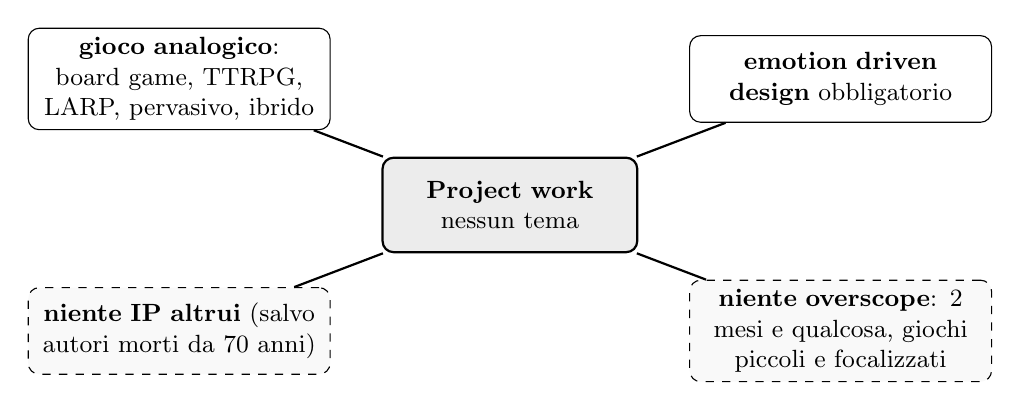
\begin{tikzpicture}[
    font=\small,
    centro/.style={draw, thick, rounded corners, fill=gray!15, text width=3.0cm,
      align=center, minimum height=1.2cm},
    vincolo/.style={draw, rounded corners, text width=3.6cm, align=center,
      minimum height=1.1cm, fill=white},
    no/.style={draw, dashed, rounded corners, text width=3.6cm, align=center,
      minimum height=1.1cm, fill=gray!5},
    linea/.style={thick}
  ]
  \node[centro] (c) at (0,0) {\textbf{Project work}\\ nessun tema};
  \node[vincolo] (a) at (-4.2,1.6) {\textbf{gioco analogico}: board game, TTRPG,
    LARP, pervasivo, ibrido};
  \node[vincolo] (b) at (4.2,1.6) {\textbf{emotion driven design}
    obbligatorio};
  \node[no] (d) at (-4.2,-1.6) {\textbf{niente IP altrui} (salvo autori morti da
    70 anni)};
  \node[no] (e) at (4.2,-1.6) {\textbf{niente overscope}: 2 mesi e qualcosa,
    giochi piccoli e focalizzati};
  \foreach \x in {a,b,d,e} { \draw[linea] (c) -- (\x); }
\end{tikzpicture}
\caption{Il \emph{mandate} del project work: due cose da fare (in alto) e due da
non fare (in basso, tratteggiate). Ricostruzione schematica della slide di
Daniele.}
\label{a7:fig:mandate}
\end{figure}

% ---------------------------------------------------------------------
\section{I gruppi}
\label{a7:sec:gruppi}

Poi i gruppi, tre gruppi da tre (tabella~\ref{a7:tab:gruppi}). La scelta è dei
docenti ed è ``insindacabile'', ma è basata sulle attività e sui task fatti
finora, ``sulla base di quello che vi abbiamo fatto fare negli ultimi giorni, come
lezioni, sulla vostra task e su quello che è stato un po' il nostro modo di
vedere''. Si è cercato di bilanciare anche gli \textbf{impegni di lavoro} di
ciascuno.

\begin{table}[htbp]
\centering
\begin{tabular}{@{}ll@{}}
\toprule
\textbf{Gruppo} & \textbf{Componenti} \\
\midrule
Gruppo 1 & Giordano, Nicola, Rita \\
Gruppo 2 & Gianmarco, Tancredi, Lorenzo Vergata \\
Gruppo 3 & Tiziana, Angelo, l'altro Lorenzo \\
\bottomrule
\end{tabular}
\caption{I gruppi del project work come li annuncia Daniele\protect\footnotemark.}
\label{a7:tab:gruppi}
\end{table}
\footnotetext{La trascrizione dice ``Giordano, Nicole, Rita, gruppo 2 Gianmarco,
Tancredi e Lorenzo V, gruppo 3 Tiziana, Angelo e Lorenzo''. ``Lorenzo V'' è Lorenzo
Vergata, come confermano poi i messaggi tra lui e Tancredi durante la pausa;
``Nicole'' è Nicola, a cui più tardi Beatrice dice che è nel gruppo ``con Giordano e
Rita''.}

Il progetto va sviluppato \textbf{durante il corso}: ``non vanno bene idee
pregresse, non portate nei vostri gruppi idee precedenti''. Le idee si sviluppano
insieme agli altri.

% ---------------------------------------------------------------------
\section{Le regole per lavorare in gruppo}
\label{a7:sec:regole}

Prima di lasciare la lezione a Beatrice, Daniele dà ``altri consigli per gli
acquisti''.

\paragraph{Rispettarsi.} ``La maggior parte del lavoro di un gruppo di sviluppo è di
\textbf{soft skill} più che di skill''. Bisogna capire come collaborare: se qualcuno
ha impegni di lavoro e fa fatica a garantire del tempo, ``partite da quello''. Non
si parte con ``un progetto grande come un castello disneyano'' per poi trovarsi
senza tempo; ci si dice invece ``io posso lavorare solo in questi momenti, lui o lei
solo in questi momenti'', e si cerca di fare ``qualcosa che abbia senso fare per il
tempo che abbiamo a disposizione''.

\paragraph{Taggare i docenti.} In caso di problemi si scrive ai docenti su
\textbf{Discord}, ma \textbf{taggandoli}: ``non lasciate messaggi senza taggarci,
se no li vedo una settimana dopo''. Oppure su \textbf{Telegram}.

\paragraph{Usare subito questi giorni.} Questi giorni vanno usati per il
\emph{brainstorming}: il tutoraggio con Ruggero è a breve (Daniele parla di ``48
ore'' per impostare il lavoro e capire che cosa fare).

\paragraph{Lavorare nel Drive.} Questa è una regola \textbf{obbligatoria}. Nel
Drive condiviso del corso ci sono le cartelle ``attività in classe'', ``dispense'',
``materiali didattici'' e ``project work''; dentro ``project work'' Daniele crea
tre cartelle, \textbf{gruppo 1}, \textbf{gruppo 2} e \textbf{gruppo 3}. Lavorare nel
Drive vuol dire evitare il più possibile di creare file fuori e caricarli dopo:
si aprono i Google Document lì e si lavora \textbf{in cloud}. Il motivo: se un
gruppo ha problemi e Daniele vuole aiutarlo, ha bisogno di vedere il
\textbf{processo mentale}, cioè che cosa è stato fatto nel documento, ``lo
\textbf{storico} del documento''. Un PDF o un \texttt{.docx} caricati così come
sono non hanno storico. Le cartelle vanno organizzate al meglio possibile; per
qualsiasi problema, ``basta chiedere''.

\paragraph{La dispensa sul brainstorming.} A seguito di questa lezione, ``tra stasera
e domani mattina'', Daniele registrerà una \textbf{dispensa}: il pezzo che venerdì
non c'è stato modo di fare, sul \emph{brainstorming} e sulla ricerca e sviluppo
``lato marketing'' e sugli strumenti di marketing nella ricerca e sviluppo. Metterà
a disposizione le slide e un video, con le slide del \textbf{brainstorming
strutturato}.

Nessuna domanda (``molti pollicioni, va bene''). Daniele ringrazia Bea ``per il
supporto e la condivisione'', saluta (``ci vediamo sicuramente il 12 di
ottobre'') e lascia la lezione.

% ---------------------------------------------------------------------
\section{Perché facciamo game design: due obiettivi}
\label{a7:sec:obiettivi}

``Ciao gruppo''. Beatrice comincia dando un po' di contesto: il corso è alla
\textbf{seconda edizione}, ci sono cambiamenti rispetto alla prima, e i docenti
stanno cercando di capire ``come rendervi il lavoro più agile e fattibile
possibile''. Nelle slide di oggi c'è molto, ``sarò onesta, credo troppo per la
lezione di oggi'', e quello che non si farà si riprenderà nella lezione successiva.
Il programma: ``mettere le mani in pasta'' per prepararsi ad affrontare un lavoro di
design; un po' di \emph{brainstorming} (da approfondire con i materiali di Daniele);
e una sorta di percorso di creazione di un gioco con un piccolo \textbf{esercizio di
design sprint}, a cui sarà dedicata la maggior parte della lezione. Alla fine del
corso i docenti chiederanno anche dei \textbf{feedback} su come è andato tutto.

Prima, però, un ``cappellino introduttivo'' sul \textbf{perché facciamo design}, già
anticipato nelle lezioni precedenti. Ci sono \textbf{due entità} che in questo
contesto si chiamano \textbf{obiettivi di design}:
\begin{enumerate}
  \item l'\textbf{obiettivo del gioco}, della produzione che si fa;
  \item l'\textbf{obiettivo personale} di chi progetta.
\end{enumerate}

\paragraph{L'obiettivo del gioco.} Un obiettivo di design del gioco, o del momento in
cui si sta facendo design, ha molte possibilità: raccontare un'esperienza di vita,
esplorare meccaniche o dinamiche, e così via; gli esempi della slide sono ``buttati
lì, sempre in brainstorming''. Si può decidere di fare un gioco per $N$ motivi, alcuni
personali e altri esterni al proprio bisogno personale.

Il punto è che \textbf{il motivo per cui affrontiamo la creazione di un gioco cambia
anche come progettiamo}. Beatrice vuole invitare la classe a ragionare su queste
cose, che spesso restano \textbf{ragionamenti interni} e invece è importante che
siano anche \textbf{condivisi}.

\paragraph{L'obiettivo personale.} L'obiettivo personale è semplice: rispondere alla
domanda \textbf{``perché sto facendo questo gioco?''}. Beatrice propone
\textbf{quattro categorie}, ``ma ce ne sono molte altre'', e probabilmente ne
emergeranno di nuove col crescere della disciplina; per la classe, i macro-obiettivi
saranno verosimilmente questi (figura~\ref{a7:fig:obiettivi}).
\begin{enumerate}
  \item \textbf{Voglio pubblicare un gioco.} Come gruppo di lavoro o come persona,
        voglio parlare a degli editori e pubblicare. Sotto questo cappello stanno sia
        la \textbf{pubblicazione con un editore} sia
        l'\textbf{auto\-pubblicazione}.
  \item \textbf{Voglio esprimere me stesso o me stessa.} È ``molto sottovalutato,
        troppo sottovalutato'': il gioco è uno strumento di espressione molto grande,
        che coinvolge anche altre persone. Magari non si vuole pubblicare né vendere,
        ma trasmettere davvero qualcosa che si è vissuto, qualcosa che si vuole
        raccontare; o si fa attivismo politico e si vuole un'attività che
        sensibilizzi sull'ecologia o su altri temi.
  \item \textbf{Voglio formare, informare o sensibilizzare.} Può sovrapporsi al
        punto precedente. Un gioco per insegnare meglio la matematica, per far
        conoscere un quartiere della propria città o un evento storico, per far
        crescere una competenza (aiutare le persone a parlare meglio in gruppo):
        ``$N$ situazioni di formazione''.
  \item \textbf{Voglio usare i giochi per il marketing e la comunicazione.} Portare
        l'attenzione su qualcosa: può essere un'espressione personale o una
        sensibilizzazione, ma anche un \textbf{prodotto} o un \textbf{servizio}. Lo si
        è visto con gli \emph{alternate reality game} del marketing, e in tante altre
        situazioni.
\end{enumerate}

\begin{figure}[htbp]
\centering
\begin{tikzpicture}[
    font=\small,
    domanda/.style={draw, thick, ellipse, fill=gray!15, text width=3.2cm,
      align=center, inner sep=2pt},
    ob/.style={draw, rounded corners, text width=3.3cm, align=center,
      minimum height=1.5cm, fill=white},
    freccia/.style={-{Stealth[length=2mm]}, thick}
  ]
  \node[domanda] (q) at (0,0) {\textbf{Perché sto facendo questo gioco?}};
  \node[ob] (p) at (-4.4,1.9) {\textbf{pubblicare}\\ con un editore o in
    autoproduzione};
  \node[ob] (e) at (4.4,1.9) {\textbf{esprimere me stesso/a}\\ raccontare,
    sperimentare, attivismo};
  \node[ob] (f) at (-4.4,-1.9) {\textbf{formare, informare, sensibilizzare}\\
    scuole, terzo settore, aziende};
  \node[ob] (m) at (4.4,-1.9) {\textbf{marketing e comunicazione}\\ prodotti,
    servizi, ARG};
  \foreach \x in {p,e,f,m} { \draw[freccia] (q) -- (\x); }
\end{tikzpicture}
\caption{Le quattro categorie di obiettivo personale proposte da Beatrice. ``Ce
ne sono molte altre''; esprimersi e sensibilizzare spesso si sovrappongono, e uno
stesso gioco può rispondere a più obiettivi.}
\label{a7:fig:obiettivi}
\end{figure}

% ---------------------------------------------------------------------
\section{Le competenze che ogni obiettivo richiede}
\label{a7:sec:competenze}

Ognuno di questi obiettivi personali richiede delle \textbf{competenze}, che ci si
fa ``in corso d'opera''. I docenti non si aspettano che gli studenti approfondiscano
ogni slide durante il corso, ma vogliono dire una cosa: se si crea un gioco, tutta
l'analisi di cui si è parlato (del mercato, delle persone, del target) va tenuta in
considerazione \textbf{in funzione dell'obiettivo}. Ogni obiettivo ha un modo
diverso di guardare il gioco e di produrlo. La slide mostra una ``carrellata'' di
competenze e conoscenze (tabella~\ref{a7:tab:competenze}).

\paragraph{Pubblicare con un editore.} Sono emerse domande anche dalla classe su come
capire che cosa sia meglio fare. Bisogna \textbf{conoscere il mondo della produzione}
di giochi da tavolo, di giochi di ruolo e di eventi ludici: chi esiste, che cosa fa,
a che prezzi mette fuori le cose, che tipo di prodotti vende già; se ci si riesce,
quante copie vengono vendute, quante persone comprano un biglietto. E
\textbf{conoscere le persone}: non solo ``c'è la casa editrice con il nome X'', ma
``all'interno ci lavorano X, Y, Z''. Partecipare agli eventi, mettersi in
connessione: sono tutte competenze, orientate a capire \textbf{come inserirsi} nelle
realtà che possono avere interesse a pubblicare.

\paragraph{Autoprodursi.} Le logiche sono diverse. Il mondo editoriale va conosciuto
comunque, perché in questo caso sono \textbf{competitor}; ma bisogna ragionare di più
verso il \textbf{pubblico}: capire come arrivare al momento in cui le persone
acquistano. Quindi parlare con gli utenti, affinare il marketing, analizzare i
competitor. E i competitor non sono solo quelli che fanno la stessa attività: per un
\textbf{evento dal vivo} un competitor può essere una fiera o un concerto, non per
forza un'attività di gioco; per un \textbf{gioco da tavolo formativo} un competitor
può essere un \textbf{corso}, non per forza un altro gioco. ``Immaginate i
competitor un po' più ad ampio spettro''. Infine, tutta una serie di informazioni
``non scontate'' e ``spesso prese sotto gamba'': \textbf{fiscalità e normative}.

\paragraph{Il GDPR: un'anticipazione.} Su questo, nella prossima lezione, Beatrice
farà ``un piccolo cappello'' sulle basi del \textbf{GDPR}, per poter raccogliere i
dati degli utenti e ricontattarli. È utile qualunque sia l'obiettivo: è sempre utile
avere, in una forma che permetta di risentirle, i dati delle persone con cui si è
venuti in contatto, che magari hanno testato il gioco, per tornare a scrivergli e
capire una serie di cose.

\paragraph{Esprimere se stessi.} Per sperimentare, per esplorare: qui ci sono
competenze ``spesso non raccontate, perché meno orientate al mercato'', che
riguardano \textbf{come trasmettiamo i contenuti} che vogliamo portare. È il lavoro
di \textbf{emotional design}, che ``sembra complicatissimo'', o comunque difficile da
definire; lo è, perché cambia per ogni gioco, ma col tempo si raffina sempre di più.
Chi vuole usare il gioco come sperimentazione personale, come linguaggio di dialogo
personale, deve capire bene quali sono i propri obiettivi: può essere ``voglio
comunicare la mia storia personale'', ma anche ``voglio trovare persone a me
affini'', o, ``banalmente'', ``voglio essere la persona che ha fatto il gioco più
conosciuto sulle \textbf{lumache da prato}''. Se è quello che si vuole raggiungere,
va bene: capito bene l'obiettivo, si capisce meglio tutto il resto, cioè
\textbf{che cosa voglio dire, a chi dirlo e perché} voglio dire determinate cose.

\paragraph{Formare, informare, sensibilizzare.} ``C'è un mondo'' su come si fa questo
design; qualcosa si vedrà nella prossima lezione, con le \textbf{escape room} e le
escape room formative. Per capire il mercato che può pagare queste attività, secondo
l'esperienza di Beatrice (``che non è onnisciente, ma è abbastanza puntuale al giorno
d'oggi''), le macro-voci in cui ci sono dei soldi, escludendo
l'\textbf{autofinanziamento} (che lei mette in una voce a sé), sono tre:
\begin{itemize}
  \item il \textbf{terzo settore} e i \textbf{bandi};
  \item il mondo delle \textbf{scuole} e della \textbf{formazione};
  \item la \textbf{formazione aziendale}: \emph{learning and development}, risorse
        umane e simili.
\end{itemize}
Sono tre mondi con logiche ``completamente diverse'' da quelle viste prima, e
Beatrice non ci si sofferma, perché non è il fulcro del corso. Ma già queste voci
bastano per sapere dove approfondire, se si vuole fare un gioco formativo: che cos'è
il terzo settore e che cosa significa proporgli dei giochi; che cosa sono i bandi
pubblici e quali enti li finanziano; e lo stesso per le scuole e per le aziende. E
poi c'è ``il magico mondo della \textbf{formazione finanziata}'', che sta sempre
sotto il cappello delle risorse umane: già googlando queste due parole si trovano
molte situazioni in cui si inserisce la proposta di giochi.

\paragraph{Il marketing.} Qui la parte principale da sapere è quella già vista
sull'\textbf{analisi del target} e sull'individuazione delle persone da coinvolgere.
Beatrice non si sofferma, perché secondo lei il marketing ``arriva dopo'': quando si
è progettato un po' di più (vale anche per la formazione) e si è sperimentato quello
che si è in grado di fare, allora si possono immaginare giochi per il marketing, che
sono giochi che portano l'utente a fare determinate cose. Per chi vuole approfondire,
la cosa principale è questa: si parla con delle \textbf{aziende}, e le aziende,
``anche le più virtuose'', hanno l'obiettivo di ``fare dei soldini''. Bisogna saper
rispondere alla domanda \textbf{``come aiuta l'azienda a fare più soldi?''}. I casi
sono due: \textbf{aumenta le vendite}, oppure fa aumentare \textbf{quanto l'azienda è
conosciuta}, o, se è conosciuta male, ne modifica in positivo la
\textbf{reputazione}. ``Non è un mondo bellissimo, ma è un mondo che esiste'': giochi
di questo tipo esistono tantissimo, e spesso non sono neanche raccontati come tali.
Beatrice lo dice perché magari si ha ``il gioco migliore del mondo'' e non si sa come
pagarsene lo sviluppo: questo può essere un modo.

\begin{table}[htbp]
\centering
\begin{tabular}{@{}p{3.0cm}p{9.6cm}@{}}
\toprule
\textbf{Obiettivo} & \textbf{Che cosa bisogna conoscere} \\
\midrule
Pubblicare con un editore & il mondo della produzione (chi c'è, che cosa fa, a che
prezzi, quanto vende); le persone dentro le case editrici; eventi e contatti \\
Autoprodursi & il mondo editoriale come competitor; il pubblico; marketing;
competitor ``ad ampio spettro'' (una fiera, un concerto, un corso); fiscalità e
normative; GDPR \\
Esprimere se stessi & come trasmettere i contenuti; \emph{emotional design}; che
cosa voglio dire, a chi e perché \\
Formare e sensibilizzare & terzo settore e bandi; scuole e formazione; formazione
aziendale (\emph{learning and development}, risorse umane); formazione finanziata \\
Marketing & analisi del target; ``come aiuta l'azienda a fare più soldi?'':
vendite, notorietà, reputazione \\
\bottomrule
\end{tabular}
\caption{Le competenze per obiettivo personale, ricostruite dalla carrellata di
Beatrice.}
\label{a7:tab:competenze}
\end{table}

\paragraph{Lo stesso gioco, più obiettivi.} Uno stesso gioco può rispondere a più
obiettivi. Si fa un gioco formativo, o un gioco per esprimersi, e si scopre che
potrebbe essere venduto a un'azienda, rispondere a un bando, entrare
perfettamente nel catalogo di un editore estero ``che non conoscevate fino a ieri'',
o di un editore italiano conosciuto in fiera. Quello che interessa a Beatrice è che
gli studenti abbiano chiari \textbf{gli interessi del mondo a cui parlano}, quando
hanno un gioco in progettazione o già fatto. Se si è consapevoli degli interessi
degli altri e del proprio obiettivo personale, ``diventa molto più facile il
dialogo''. Riuscire poi a vendere e ``imbroccare le cose giuste'' è un altro tema;
ma questi due elementi vanno avuti \textbf{prima}.

\paragraph{Approfondimento: il perché del designer.} Il tema dell'obiettivo personale
ha un parallelo in \emph{The Art of Game Design} di Jesse Schell, che apre il libro
non dal gioco ma dal designer stesso (``in the beginning, there is the designer''),
e più avanti dedica capitoli interi al rapporto con il \emph{cliente} e al
\emph{pitch}, cioè proprio al ``dialogo'' con gli interessi altrui di cui parla
Beatrice. Nella lezione, però, la distinzione tra
\emph{obiettivo del gioco} e \emph{obiettivo personale} ha soprattutto una funzione
pratica: è il primo argomento della chiacchierata iniziale del design sprint.

% ---------------------------------------------------------------------
\section{Il design sprint}
\label{a7:sec:sprint}

``Ora sono andata un po' veloce, e sono comunque lenta rispetto agli orari'':
Beatrice passa all'esercizio. Condivide un altro file (``che voi vedete bruttarello
qui e che poi vi caricherò''); chi non lo legge può mandarle ``un'emoji triste o
buffa''. Ha preparato \textbf{due moduli}; quello di adesso è su \textbf{come fare una
sessione di design sprint}.

\paragraph{Che cos'è.} Il design sprint si può usare per $N$ cose: ``dal decidere
come arredare casa a come risolvere il problema di non avere abbastanza soldi per
fare la spesa'', per qualunque problema. \textbf{Non è uno strumento nato per il game
design}: è nato per ragionare su problemi di progettazione e cercare soluzioni di
design. Beatrice lo ha \textbf{adattato all'uso sui giochi}, e lo ha diviso in
\textbf{fasi}, perché sono le fasi che invita i gruppi a provare a seguire. Il file
verrà caricato nella cartella condivisa degli strumenti. Oggi racconterà la prima
fase, ma la salterà, e si partirà dalla seconda.

\paragraph{Un invito, non un obbligo.} È ``uno strumento in più che vi dà una
direzione in caso la direzione non riusciate a trovarla in breve tempo''. Beatrice lo
dice apertamente: l'anno scorso alcuni gruppi hanno investito molto tempo in alcune
fasi della progettazione e non sono riusciti a concludere il gioco. Quest'anno si
vuole evitarlo, e per questo ci sono \textbf{due strumenti}: questo, e quello che si
vedrà alla fine di questa lezione e all'inizio della prossima, cioè tutte le voci che
compongono la progettazione di un gioco, per avere una \textbf{visione d'insieme} e
poter dire: ``abbiamo queste settimane prima del pitch e questi mesi prima della
consegna''. Ognuno ha un lavoro, una famiglia, dorme, mangia, fa cose che occupano
tempo: bisogna farsi ``dei conti pratici'', un tot di ore per una parte e un tot per
un'altra.

\paragraph{Il project management che non c'è.} Tutto questo fa parte del
\textbf{project management} di un progetto, e Beatrice avverte che nel mondo del
lavoro, ``nel gaming perlomeno'', \textbf{non esiste}: nella slide in cui sono state
presentate tutte le professioni non c'è un \emph{project manager} dei giochi, perché
le aziende sono ``ancora un po' in costruzione'' su questo lato; quelle italiane
almeno, mentre all'estero ci sono casi molto diversi, e nel videogioco funziona in un
altro modo. Questi strumenti vanno conosciuti per essere più consapevoli di
\textbf{come si funziona come persone}, preparandosi al fatto che il mondo esterno
non sempre segue logiche di organizzazione e ``più spesso bisogna un po' navigare le
onde''. Per il corso, però, sono molto utili: quando il gruppo ``per un attimo si
perde'', si può tornare a fare il punto con questi strumenti.

\subsection{Le fasi del file}
\label{a7:sec:fasi-file}

Beatrice scorre i ``titoloni'' del documento (figura~\ref{a7:fig:sprint}).
\begin{enumerate}
  \item \textbf{La chiacchierata iniziale}, che oggi si salta (si veda sotto).
  \item \textbf{Definire l'obiettivo di gruppo} del gioco: proposte e votazioni.
  \item Una piccola sessione di \textbf{ricerca e sviluppo} basata sull'obiettivo.
  \item Una prima sessione di \textbf{brainstorming} su quello che emerge, per
        rispondere all'obiettivo.
  \item La \textbf{valutazione} di tutto il brainstorming: che cosa si tiene e che
        cosa si butta, di tutte le idee uscite.
  \item Da lì in poi, l'\textbf{assegnazione dei ruoli}: chi fa cosa, con che tempi.
\end{enumerate}
Oggi si faranno le fasi dalla seconda in poi, fingendo che la classe sia un unico
grande gruppo di \textbf{nove persone} che inventa un gioco: ``faremo tutto quello
che serve per fare un brainstorming per avere il pitch del gioco''. Sarà un gioco
``del gruppo tutto'', quindi non lo si potrà portare a conclusione nel corso: serve
ad allenarsi con lo strumento.

\begin{figure}[htbp]
\centering
\begin{tikzpicture}[
    font=\small,
    fase/.style={draw, thick, rounded corners, text width=2.5cm, align=center,
      minimum height=1.3cm, fill=white},
    oggi/.style={fase, fill=gray!15},
    saltata/.style={fase, dashed, fill=gray!4},
    freccia/.style={-{Stealth[length=2mm]}, thick},
    nota/.style={font=\scriptsize\itshape, text width=2.5cm, align=center}
  ]
  \node[saltata] (f0) at (0,0) {chiacchierata iniziale (30 min)};
  \node[oggi, right=0.5cm of f0] (f1) {obiettivo del gioco: post-it e voto};
  \node[oggi, right=0.5cm of f1] (f2) {ricerca e sviluppo};
  \node[oggi, right=0.5cm of f2] (f3) {brainstorming su meccaniche, tipo,
    narrazione, setting};
  \node[oggi, below=1.1cm of f3] (f4) {voto, poi mappa impatto-sforzo};
  \node[oggi, left=0.5cm of f4] (f5) {percorso dell'utente};
  \node[fase, left=0.5cm of f5] (f6) {chi fa cosa, con che tempi};
  \node[fase, left=0.5cm of f6] (f7) {progettazione e sviluppo};
  \draw[freccia] (f0) -- (f1);
  \draw[freccia] (f1) -- (f2);
  \draw[freccia] (f2) -- (f3);
  \draw[freccia] (f3) -- (f4);
  \draw[freccia] (f4) -- (f5);
  \draw[freccia] (f5) -- (f6);
  \draw[freccia] (f6) -- (f7);
  \draw[freccia, dashed] (f7.north) -- node[midway, right=2pt,
    font=\scriptsize, align=left] {quando ci si perde:\\ di nuovo al voto}
    (f1.south west);
  \node[nota, above=0.1cm of f0] {saltata a lezione};
\end{tikzpicture}
\caption{Le fasi del design sprint adattato da Beatrice per il corso. In grigio le
fasi toccate a lezione (alcune solo raccontate per mancanza di tempo); la
chiacchierata iniziale è saltata. La freccia tratteggiata riassume il consiglio
``quando vi perdete, andate a votazione''. Ricostruzione schematica del file.}
\label{a7:fig:sprint}
\end{figure}

\paragraph{Una scaletta per il corso, non il design sprint.} Beatrice lo ripeterà più
avanti, a Nicola: la scaletta \textbf{non è una fase standard}, ``non voglio che vi
portiate a casa che il design sprint è tutto così, sempre, a queste fasi''. Prende
delle metodologie e le porta in una scaletta pensata per il corso.

\subsection{La chiacchierata iniziale}
\label{a7:sec:chiacchierata}

La prima fase è un \textbf{allineamento di gruppo}, e oggi si salta. Le domande:
\begin{itemize}
  \item quali sono i nostri \textbf{obiettivi personali} (quelli visti prima)?
        ``Magari il mio obiettivo in questo corso è provare a sperimentare. Oppure
        Lorenzo vuole fare un gioco per provare a venderlo da qualche parte, oppure
        io voglio fare un gioco per raccontare la storia della mia famiglia''.
        Allinearsi non vuol dire che sarà quello che si porterà a casa, ma che si
        conoscono i desiderata degli altri e c'è uno spazio per raccontare i propri;
  \item \textbf{che competenze ho}? A quali progetti ho già lavorato, e che cosa
        facevo in quei progetti?
  \item la ``domandona'': in questo corso voglio lavorare sulle \textbf{stesse
        competenze} su cui ho lavorato in passato, o ci sono attività che non ho
        ancora esplorato, che non ho mai fatto e vorrei esplorare qui? ``Non ho mai
        scritto testi, ma qua mi andrebbe di provare'', ``non ho mai fatto
        illustrazioni e qua mi andrebbe di vedere'': qui si può fare, e conviene
        capire in che ruolo mettere le proprie competenze. (Beatrice corregge anche
        un refuso nel file, in diretta.)
\end{itemize}
Per gruppi di tre persone, \textbf{30 minuti} bastano e avanzano: uno scambio in cui
``ognuno sa la situazione delle altre persone''. Beatrice invita a farla quando
inizierà il lavoro di gruppo.

\paragraph{Approfondimento: lo Sprint di Google Ventures.} Il \emph{design sprint}
nella forma più nota è quello descritto da Jake Knapp, con John Zeratsky e Braden
Kowitz, nel libro \emph{Sprint} (2016), nato a Google Ventures: cinque giorni per
passare da un problema a un prototipo testato con utenti reali, con passaggi molto
simili a quelli della lezione (mappare il problema, raccogliere ispirazioni,
proporre soluzioni individualmente e in silenzio, votare con adesivi a pallino,
decidere). L'adattamento di Beatrice ne conserva il cuore (lavoro individuale
silenzioso, presentazione, voto a pallini, tempi rigidi) ma lo piega ai tempi e agli
scopi di un corso: niente giornate intere, e la prima fase dedicata alle persone del
gruppo, non al problema.

% ---------------------------------------------------------------------
\section{La lavagna di Canva}
\label{a7:sec:canva}

``Ora vi condivido questa fantastica lavagna''. Per il \emph{brainstorming} ci sono
``tantissimi'' strumenti e modalità; oggi si usa il design sprint come modalità e una
\textbf{lavagna di Canva} come strumento.

\paragraph{Entrare.} Il link nella chat non è cliccabile, né si riesce a copiarlo
(``nemmeno copia e incolla''). Qualcuno lo copia a mano nella barra del browser e
riesce a entrare; un altro lo mette su Discord, dove ``funziona'', anche se a qualcuno
risulta che dal link di Discord non ha l'autorizzazione (``essendo che il link l'ho
copiato io, magari non ci sono i permessi''). Alla fine Beatrice crea un link
accorciato, ``più dettabile'' (\texttt{urli.it/31GRXQ}, secondo la trascrizione).

\paragraph{Gli strumenti in generale.} Canva è uno strumento per sessioni di
\emph{brainstorming} simile a molti altri; un altro è \textbf{Miro}, ``ma ce ne sono
davvero tanti''. Beatrice usa Canva perché è il più comodo per lei. L'impostazione
della lavagna \textbf{simula un incontro dal vivo}: le attività di oggi si possono
fare in digitale, a distanza, con uno strumento di questo tipo, oppure dal vivo con
\textbf{carta e penna}, un tavolo dove appoggiare i bigliettini, un muro dove
attaccare i post-it. ``Ve lo dico perché può essere utile anche per il futuro''.

\paragraph{Come si usa.} Beatrice ha ``loccato'' (bloccato) gli elementi della
lavagna, così che nessuno sposti per errore le cornici; si può selezionare e
zoomare liberamente (avvicinandosi le lavagne ``diventano più grandi''), ma bisogna
stare attenti a non cancellare il lavoro degli altri. Per cancellare: si seleziona
l'elemento e si preme il tasto di cancellazione, oppure il piccolo cestino nel menu
dell'elemento. Gli strumenti utili sono nel \textbf{menu a sinistra} di Canva, che ha
sette voci (Canva AI, Modelli, Elementi, Testo, Brand, Caricamenti,
\textbf{Strumenti}); sotto \textbf{Strumenti} (l'icona con una ``pennina'') ci sono,
tra gli altri, il \textbf{testo} e i \textbf{foglietti adesivi}: ``veri e propri
post-it, come quelli che usereste dal vivo''. Si sceglie un colore, il post-it compare,
lo si ingrandisce o rimpicciolisce e ci si scrive sopra.

\paragraph{Le prove.} La prova serve anche ad allinearsi sullo strumento, ed è
movimentata. I post-it compaiono uno dopo l'altro (``Giordano, anche Lorenzo'',
``vedo una C'', ``Rita sta scrivendo''); Gianmarco entra senza il suo account e
compare come ``Leone Marino'', uno dei nomi di animale che lo strumento assegna
agli utenti anonimi\footnote{La trascrizione dice ``è come l'anonimo di Giuseppe'':
con ogni probabilità il riferimento è agli ``animali anonimi'' con cui Google e
altri servizi mostrano chi partecipa senza account.}. Si scopre che se la
lavagna di base è bloccata non si riesce a scrivere nei post-it (``io l'ho imparato
adesso, perché credevo non funzionasse così''), e Beatrice sblocca. Qualcuno sposta
per sbaglio l'intera cornice (``oh mio Dio, sono uscito, e qualcuno ha spostato tutta
la lavagna''), qualcuno ha post-it finiti fuori dalla lavagna o giganteschi, una
studentessa (``una grafica fissata con l'impaginazione'') prova a riallineare
tutto. Angelo, che è collegato \textbf{dal cellulare}, non riesce a trascinare il
post-it (``non me lo fa trascinare''); Beatrice lo guida passo per passo e alla fine
decide di creargli lei dei post-it con il proprio nome sopra, che Angelo userà
(``ci ricorderemo che i tuoi post-it sono quelli con il nome di Beatrice''), anche
se poco dopo Angelo riesce a crearne uno da solo (``ce l'ho fatta'').
``Dal telefono è anche più complicato, è normalissimo''. Beatrice avverte che
\textbf{Miro è un po' più intuitivo} di Canva, e che servirà molto spazio: il gioco di
fare le cose piccole e zoomare sarà utile soprattutto nella ricerca e sviluppo.

\paragraph{Lo strumento conta il giusto.} ``Di tutto questo, lo strumento ci interessa
il giusto'': si può usare Miro, si possono scrivere le cose a mano. \textbf{Ci
interessa il procedimento}.

% ---------------------------------------------------------------------
\section{Prima fase: che obiettivo vorrei dare a questo gioco?}
\label{a7:sec:fase1}

La domanda della prima fase è \textbf{``che obiettivo vorrei dare a questo
gioco?''}. Le regole:
\begin{itemize}
  \item ognuno scrive \textbf{al massimo tre risposte}, e almeno una;
  \item \textbf{una risposta per post-it};
  \item non è il genere del gioco e non sono le meccaniche: è ``più a volo
        d'aquila'', quello che si vorrebbe che il gioco ottenesse; può riguardare
        anche le \textbf{emozioni}, cioè che cosa far provare alla persona che gioca.
\end{itemize}
Gli esempi del file mescolano apposta livelli diversi: ``un gioco formativo per
insegnare l'inglese'', ``un gioco con dei pinguini blu'', ``un GDR per sensibilizzare
sulla lotta di classe'', ``un gioco fantasy sulla vendetta'', ``un gioco con delle
pedine gigantesche'', ``un gioco che faccia esplorare un quartiere''.

\paragraph{I timer.} E qui la cosa da ricordare di tutto il procedimento:
\textbf{mettere i timer}. Nei processi creativi di gruppo, e probabilmente lo si è già
visto succedere, ci si fa prendere da quello che sta avvenendo, dai dialoghi, dalle
idee che emergono. Beatrice richiama la lezione precedente su \textbf{divergenza e
convergenza}: c'è un momento in cui si apre, si esplora, si buttano idee; ma ``a un
certo punto bisogna \textbf{quagliare}''. Darsi un tempo di orologio dice fino a
quando si esplora; quando suona il timer, bisogna riportare in ordine la situazione.
``È la cosa importante di tutto il processo: dare dei tempi e provare a
rispettarli''. Il primo timer è di \textbf{5 minuti} (``dai 5 ai 10'').

\paragraph{Gianmarco arriva.} Gianmarco, ``arrivato un po' in corsa'', chiede il
contesto: si può buttare qualsiasi idea? È un esercizio, risponde Beatrice, per
imparare a fare \emph{brainstorming} e poi mettere in ordine le idee: ``vai pure
libero''.

\paragraph{La parola proibita.} Mentre scrivono, Rita avverte i compagni: qualcuno
ha scritto \emph{divertire} su un post-it, e ``dovremmo evitare di usare questo
verbo''\footnote{Il riferimento è alla regola, ricorrente nel corso, per cui ``far
divertire'' non è un obiettivo di design: è troppo generico per orientare le
scelte.}, ``conviene modificarlo prima che lo veda qualcuno'' (Ruggero, si
capisce). Beatrice: ``Io non dirò niente, però è un ottimo consiglio''. Del resto,
aggiunge, sono idee che non verranno condivise con gli altri docenti: è un esercizio
per imparare la procedura, che non è neanche detto si userà esattamente così. Le idee
di oggi possono avere vita propria e crescere, ``ma non in questo corso'': i gruppi
del progetto partiranno da zero.

% ---------------------------------------------------------------------
\section{Il racconto delle idee}
\label{a7:sec:racconto}

Prima della votazione, che Beatrice anticipa (si veda la
sezione~\ref{a7:sec:votazione}), \textbf{ognuno racconta che cosa ha scritto} e dice
\textbf{dove sono} i suoi post-it, così che tutti possano trovarli sulla lavagna. In
questa fase valgono due regole:
\begin{itemize}
  \item le altre persone possono fare \textbf{solo domande}: chiarimenti su che cosa
        si intende, su perché è emersa un'idea; ``tutte le domande che vi vengono in
        mente vanno benissimo'', anzi Beatrice invita a farle, perché ``c'è ancora
        tanto che può uscire'';
  \item \textbf{niente commenti}, ``né nient'altro''. Se non si hanno domande, non si
        dice nulla.
\end{itemize}
E Beatrice si fa da parte: ``fate finta che io non esista''. Ricorderà solo di dire
dove sono i post-it; il gruppo deve autogestirsi, come in un vero lavoro di gruppo
in cui nessuno dà la direzione. Poi si accorge di aver dimenticato il timer anche
qui: tutte le idee vanno raccontate in circa \textbf{15 minuti}, ``tenetene conto
quando fate le domande, quando rispondete, quando raccontate''.

\subsection{Rita}
\label{a7:sec:idee-rita}

Rita (post-it arancione, rosso e giallo, sovrapposti nell'angolo in alto a sinistra)
ha scritto tre idee.
\begin{description}
  \item[Un gioco educativo.] Si è avvicinata a questo mondo con l'idea di dare
        qualcosa in più alle nuove generazioni: è quello che l'ha spinta a diventare
        game designer.
  \item[Un gioco che costringe le persone a collaborare.] Quando la collaborazione è
        necessaria per raggiungere un obiettivo, bisogna affrontare problemi con se
        stessi e con gli altri, e questo è costruttivo e stimolante per tutti. È anche
        il suo approccio alla vita: ``condividere, collaborare per imparare''.
  \item[Un gioco sull'arte.] È la sua più grande passione: avvicinare le persone a
        un'arte ``non proiettata verso l'IA''.
\end{description}
Le domande. Il gioco sull'arte è sulla storia dell'arte, i grandi pittori, o un gioco
in cui \textbf{le persone fanno gli artisti}? La seconda: avvicinarle alla disciplina
in maniera attiva; e in effetti, osserva Rita, potrebbe rientrare nel gioco educativo,
con le scuole. Il gioco educativo, per che età e in che contesto? Non ci ha ancora
pensato nello specifico, ma pensava a bambini che stanno crescendo, elementari e
medie: per gli adolescenti ci vuole qualcosa di più attivo e stimolante a livello
emotivo, forse un LARP. Poi chiede lei un parere a una compagna con esperienza di
questi giochi: ci sono fasce d'età più interessate a certi tipi di gioco?
``Dipende'', risponde la compagna: si sente il gruppo, e se il gioco è educativo lo
si orienta anche, per esempio decidendo se farlo competitivo o no. A lei è sempre
piaciuto \textbf{mescolare competizione e collaborazione}: le \textbf{cacce al
tesoro} sono notoriamente competitive, ma le sue richiedevano sempre una
collaborazione tra i gruppi, e alla fine \textbf{il tesoro era per tutti}: c'era la
soddisfazione di chi era arrivato primo, ma il premio era di tutti. ``Bello, e
stimolante, perché si deve collaborare per raggiungere un obiettivo''.

\subsection{Nicola arriva}
\label{a7:sec:nicola}

A questo punto entra Nicola. Beatrice gli spiega in breve che cosa sta succedendo:
un esercizio di design sprint, ``una metodologia, anzi varie metodologie che
riguardano tante forme di design, non solo quello dei giochi'', per avere una
direzione quando un gruppo si perde o non sa come allinearsi; la prima fase è
rispondere a ``che obiettivo vogliamo dare al gioco''; i compagni hanno dato tre
idee ciascuno, che ora si leggono e poi si votano. E gli dice il suo gruppo: ``sei nel
gruppo 1, con Giordano e Rita'', ``non per motivi'', lo rivedrà nelle slide che
Daniele caricherà. Nicola entra nella lavagna come ``Nick''.

Poco dopo, Nicola chiede ``un quick check-up'': si sente ``in alto mare'', ``una
zavorra''. I post-it sono già divisi in gruppi? Sono concept di personaggio o di
gioco, di ogni singola persona? Si stanno comparando? Beatrice riconosce di non
essersi spiegata abbastanza e rispiega: si sta \textbf{testando la metodologia},
fingendo di essere un unico gruppo di nove da cui deve uscire ``una bozza di gioco'';
la scaletta non è standard ma costruita per il corso; per decidere l'obiettivo del
gioco ognuno butta giù idee in silenzio sui post-it, poi le si leggono (``una fase di
brainstorming aperto'') e infine le si vota.

Nicola chiede com'è il voto: qualitativo o quantitativo? Si vota sulla quantità di
contenuto, sulla tipologia, ``un voto vale più di un altro''? Nessun voto vale più di
un altro, risponde Beatrice: ognuno avrà \textbf{sei voti}, ``immagina di avere sei
pallini adesivi'', e può metterli anche tutti sulla stessa idea. A Nicola lo schema
ricorda quello studiato in \textbf{organizzazione aziendale}, quando si avvia un
progetto; Beatrice conferma che il design sprint si usa in moltissimi contesti, ``molto
sulle soluzioni da proporre'', anche in sociologia. Nicola chiede ancora se c'è stata
una spiegazione prima del lavoro: c'è stata una piccola introduzione sui motivi per cui
si fa design (recuperabile dalle slide o dalla registrazione), e poi ci si è buttati
sulla domanda. Infine: ci sono linee guida, ``o siamo randomici''? ``Per ora è tutto
libero, rimaniamo leggerissimi''. Nicola si scusa con la classe per il tempo rubato.

\subsection{Lorenzo Vergata}
\label{a7:sec:idee-vergata}

Lorenzo Vergata (post-it sopra quelli di Rita) presenta tre idee, mentre ``qualcuno
ha mosso la lavagna'' e per un momento ``è scomparso tutto''.
\begin{description}
  \item[I funghi.] \textbf{Esplorazione del bosco per sensibilizzare sulle specie
        fungine e sul rispetto della natura}, ``semplicemente perché siamo in periodo
        di funghi'': la prima cosa che gli è venuta in mente.
  \item[Frenetismo.] Partite rapide, ``quasi caotiche dall'esterno, ma
        pseudo-organizzate dall'interno fra i giocatori''. Si è chiesto che cosa cerca,
        a 26 anni, in un gioco: non partite lunghe, ma frenesia. Frenesia, quindi,
        ``per gente neolaureata e simile''.
  \item[Paura.] Nascondino; fuggire da qualcuno all'aperto, senza luci; o in casa,
        staccando la corrente all'inizio del gioco. ``Il gioco deve far paura'':
        senza aver fatto ricerca, pensa che non ci siano molti giochi che sfruttano la
        paura dei giocatori come dinamica.
\end{description}
Le domande, e qualche commento che sfugge alla regola. L'idea della paura è pensata
come un \textbf{LARP}, all'esterno, o come un gioco da tavolo? Lorenzo pensa che il
modo più semplice di creare paura sia un LARP, ma ``nulla toglie'' di farlo da tavolo,
studiando come un gioco da tavolo possa incutere timore. Una compagna osserva che la
paura si definisce in tanti modi: \textbf{pressione}, \textbf{ansia} (più facili da
tavolo) e \textbf{jumpscare} (più da LARP); bisognerebbe dare una dimensione al
concetto, ma è ``una bella sfida''. Le ricorda quando da ragazzina giocava a
\textbf{guardie e ladri} al mare, di notte, nelle case degli amici: si creava un
clima di paura e tensione, anche perché ci si facevano gli scherzi.

Un altro studente, che gioca ``per la maggior parte del tempo'' a giochi di ruolo da
tavolo\footnote{Dal contesto, con ogni probabilità Nicola, che poco dopo si presenta
come ``un grande giocatore di TTRPG''.}, conferma che la paura è ``un fantastico
strumento'', ma pone un problema: se diventa un \textbf{gioco pervasivo}, c'è un
\textbf{danno collaterale}, cioè \textbf{spaventare chi non gioca}. ``Immagino una
persona che corre a mezzanotte in giro per Roma urlando di paura'': terrificante per
chi la vede, e si coinvolgono persone che non vorrebbero provare quella paura.
Lorenzo concorda: bisognerebbe tarare, andando più verso quello che diceva la
compagna, cioè il momento in cui sei nascosto e senti che chi ti cerca è ``letteralmente
a fianco a te'', e ti pervadono paura e ansia. Ma ``basta poco'' per tirare in mezzo
estranei: chi vede una persona che ne insegue un'altra che cerca di nascondersi
``chiama la polizia al minuto zero''. Se sono bambini di sei anni, ``stanno
giocando''; se vedi un ventenne, ``che cosa sta accadendo?''.

Infine l'esplorazione del bosco: come sarebbe, come gioco? Una guida che ti porta nel
bosco? ``Fatta sul posto è tosta'': sarebbe semplicemente una gita con un
\textbf{micologo}. Ma \textbf{da tavolo} si potrebbe fare. Sul fronte della natura si
possono inserire meccaniche che \textbf{simulano il comportamento dei funghi}: sotto
di loro c'è il \textbf{micelio}, che fa da rete di comunicazione tra le piante, e ne
potrebbe uscire un gioco ``pseudostrategico''. Sulla \textbf{commestibilità} si può
immaginare uno scontro carta contro carta, una specie di sasso-carta-forbice: ``il
fungo buono te lo annullo con questo cattivo'', mentre certi funghi che ``sembrano
buoni'' rovinano tutto il raccolto, cioè una sola carta può rovinare molte carte di
funghi buoni. ``Potrebbe anche essere frenetico, chissà''.

\subsection{Tancredi}
\label{a7:sec:idee-tancredi}

Tancredi ha scritto in modo ``molto più riassunto''.
\begin{description}
  \item[Un gioco cooperativo.] È ``un grande fan dei cooperativi'', anche piccoli,
        come \emph{Hanabi}\footnote{La trascrizione dice ``Anabis''.}, \emph{Sky Team},
        \emph{Quicksand}: gli piace molto la meccanica della cooperazione.
  \item[Un gioco per il terzo settore.] Riprende la categoria vista prima, ma senza
        grandi idee: per questo tipo di gioco sarebbe importante capire \textbf{per chi}
        lo si fa, e non sa quanto sia realizzabile nel loro caso.
  \item[Un GDR.] Non conosce praticamente per niente i giochi di ruolo, li ha
        scoperti in queste lezioni: ``perché no?'', provare a sperimentare quel
        settore.
\end{description}
Che cosa aveva immaginato per il terzo settore? Secondo Tancredi un modo sarebbe
cercare delle realtà, anche solo su internet, sui loro siti, e capire che cosa
potrebbe essere interessante per loro, ``anche se poi non glielo si propone
veramente, perché questa è un'esercitazione''; con l'obiettivo di dare una mano,
diffondere quello che fanno. Un compagno racconta (più un commento che una domanda)
di aver giocato \emph{Nemesis: Retaliation} dal vivo nella modalità semicooperativa,
con i traditori, e ora online su \textbf{Board Game Arena}\footnote{La trascrizione
scrive ``BGA'', la sigla abituale del sito.} con più o meno gli stessi amici, in
modalità cooperativa, usando la chat: ``stratosferico, così mi diverto''. Se invece
``a un certo punto uno ti dà una ginocchiata sui denti''\ldots{} Tancredi: in
associazione ``quasi mai nessuno vuole fare cooperativi'', e lui è sempre lì; gli
piacciono anche i competitivi, ma certi giochi ``vale la pena giocarli così''.

\subsection{Tiziana}
\label{a7:sec:idee-tiziana}

Tiziana (post-it sotto quelli di Tancredi) ha scritto tre idee.
\begin{description}
  \item[Un board game, di costruzione, gestionale ambientato.] Le piacerebbe fare
        esperienza di costruzione di un gioco da tavolo e non saprebbe da che parte
        cominciare (come Tancredi con i giochi di ruolo: ``non ho idea, quindi mi
        piacerebbe provare''). Un \textbf{gestionale} perché le piace l'aspetto
        gestionale, ma \textbf{ambientato}, ``non so se è una chimera''.
  \item[Un'escape room per far divertire.] ``Lo so che non devo usare divertire, ma
        non sono riuscita a trovare nessun'altra cosa'', e soprattutto far divertire
        lei mentre la costruisce. E far nascere la \textbf{collaborazione}. Dal vivo o
        da tavolo, entrambi vanno bene; il tema non lo sa. Le piacciono gli
        \textbf{indovinelli}, trovare soluzioni; ma vorrebbe enigmi \textbf{misti}, non
        tutti dello stesso tipo, perché quando sono tutti uguali diventano ``o troppo
        cervellotici o ripetitivi''.
  \item[Un gioco interattivo per far conoscere la città.] Una parte di essa, perché
        Roma ``è abbastanza gigantesca''; l'aveva immaginato coinvolgendo perfino i
        \textbf{passanti}, ``ma non so se sia fattibile''.
\end{description}
Tancredi chiede: quando parli di gestionale, hai un riferimento? Un gioco economico,
con competizione e interazione molto alte, o qualcosa di meno interattivo,
``più German''? Tiziana non lo sa: da giocatrice è più ``mi coltivo il mio orticello''
(gli economici interattivi ``non sono i miei preferiti''), ma potrebbe essere anche
interattivo: intendeva la \textbf{gestione delle risorse} in generale. La cosa
fondamentale è che sia ambientato, ``che senti di essere in quel posto''. Un
compagno le suggerisce \emph{Akropolis}, per l'ambientazione e per l'idea di
costruire la propria città con tessere di tre esagoni sovrapposte, in cui i colori che
restano in cima diventano i quartieri: un approccio per non renderlo ``troppo
gestionale German'', magari con una città costruita tutti insieme. Tiziana non lo
conosce. Beatrice interviene: si possono fare domande, ``ma non altre cose'',
altrimenti si usa troppo tempo; e manca un minuto. Tancredi: ``domanda sbagliata,
scusate''. ``Va tutto bene, siamo qui apposta per capire le dinamiche''.

\paragraph{Il timer che scade.} Manca un minuto e mancano ancora cinque persone.
Beatrice concede \textbf{altri dieci minuti}, ``ma dentro questi dieci minuti dovete
starci'': alla fine si passa allo step successivo, ``quello che è stato detto è stato
detto''. Qualcuno propone due minuti a testa; ``se volete, sì, però non posso
dirvelo io'': serve ad allenare il gruppo.

\subsection{Angelo}
\label{a7:sec:idee-angelo}

Angelo, colto un po' di sorpresa (``ci ho messo un'eternità a scriverlo, abbiate
pazienza''), ha i post-it in basso a sinistra.
\begin{description}
  \item[Un gioco di ruolo basato su un'app.] Così che la \textbf{mappa} possa essere
        continuamente aggiornata.
  \item[Un board game con possibili espansioni.] Qualcosa ``tipo \emph{Magic}, ma non
        per forza così evoluto'': ogni tanto si aggiungono carte che modificano la
        strategia.
\end{description}
Il tema è variabile, ma più fantasy o fantascienza che realismo; non aveva pensato a
un'emozione particolare. Qualcuno trova interessante il board game ``aggiornabile''.
E che cosa intende per mondo condiviso? Qualcosa come i giochi online divisi per zone
(Europa dell'Est, Europa dell'Ovest), ma molto più ristretto: si parte con
un'avventura in un \emph{medieval fantasy}, e qualcuno nella tua zona pensa a un'isola
con ambientazione \emph{steampunk} e la aggiunge al mondo, così che altri possano
andarci e ``ruolare'' in un mondo steampunk. ``Una sorta di \emph{sandbox}'':
ognuno parte dal suo stile e ci si trova in posti sempre diversi, senza un paesaggio
ripetitivo.

\subsection{Gianmarco}
\label{a7:sec:idee-gianmarco}

Gianmarco (in basso a destra) presenta tre idee.
\begin{description}
  \item[Un gioco da tavolo per bambini dai 6 agli 8 anni.] Che li spinga a
        \textbf{raccontare}, incentrato su \textbf{esplorazione e scoperta}: è la fase in
        cui i bambini iniziano a staccarsi un po' dai genitori, e nell'esplorare provano
        ``quel misto di curiosità e paura''. Con elementi grafici, un po' di
        casualità; una parte di sistema per sviluppare la \textbf{logica} e una parte di
        immagini per l'\textbf{immaginazione}.
  \item[Un board game narrativo sulla guerra.] Con le meccaniche di \emph{Mage
        Knight}\footnote{La trascrizione dice ``Image Night'' e ``Mage Night''.}:
        ``l'ho veramente buttato a caso, è una cosa senza senso''.
  \item[Un'escape room basata sul tempo.] Si deve uscire dall'ufficio, ma il tempo
        non scorre mai: bisogna risolvere enigmi per far scattare \textbf{le 17} e
        uscire finalmente.
\end{description}
Un compagno ricorda una scena dei \emph{Simpson} in cui Bart guarda continuamente
l'orologio della classe, che a un certo punto torna indietro; e suggerisce una
meccanica del tempo non in tempo reale ma a eventi, ``cose che si innescano dopo tot
minuti'' (``so che tra tre minuti mi bolle l'acqua e succede qualcosa''). Un altro
nota che è bella ``la cosa al rovescio'': di solito il timer si accorcia e ti
esaurisce, qui devi farlo andare avanti. Qualcuno trova curiosa l'idea centrale e
chiede perché le meccaniche di \emph{Mage Knight} dovrebbero rappresentare l'orrore
della guerra. Il motivo è semplice: è un periodo di guerra, a Gianmarco piace
\emph{Mage Knight} e gli piacciono i board game narrativi, ``ho messo tutto insieme,
ho fatto un po' un pastiche''.

\subsection{Nicola}
\label{a7:sec:idee-nicola}

Mancano tre minuti e mezzo per tre persone: ``un minuto a testa''. Nicola va
``rapidissimo''.
\begin{description}
  \item[Un gioco di ruolo sui tempi morti: la cucina.] È un grande giocatore di
        TTRPG, e ha notato che i giochi di ruolo da tavolo hanno regole ben stabilite
        ma quasi nessuno ha meccaniche sui \textbf{tempi morti}: in un fantasy alla
        \emph{D\&D}, quando ci si accampa ``è sempre molto randomico''. Gli
        interesserebbe un GDR basato sulla \textbf{cucina}: restare sazi per andare
        avanti nelle missioni, arrangiarsi con quello che si trova; ispirandosi a
        \emph{Dungeon Food}\footnote{Così nella trascrizione. Si tratta con ogni
        probabilità di \emph{Dungeon Meshi} (in italiano \emph{Dungeon Food}),
        manga e anime in cui gli avventurieri cucinano e mangiano i mostri del
        dungeon.}, dove si mangiano i mostri per andare avanti, perché non sempre si
        hanno le provviste.
  \item[Un gioco strategico con bluff e ruoli nascosti.] Da giocatore di ruolo, perché
        non provare uno strategico da tavolo? Lo baserebbe sulla deduzione, sul
        \textbf{bluff} e sui \textbf{ruoli nascosti}. Su una gigantesca plancia ognuno
        parte senza nazione e, ispirandosi al videogioco strategico \emph{Humankind},
        ne sblocca: Roma, che vince \textbf{conquistando}, e allora la tua strategia
        diventa conquistare; più avanti gli Egizi, che vincono \textbf{costruendo
        opere}. L'obiettivo è non far capire \textbf{in che modo vuoi vincere}: quale
        nazione, o quale somma di nazioni, sei, e quali sono i tuoi metodi di vittoria.
  \item[Un LARP sul cambiamento visibile dei personaggi.] Non ne sa niente, ma gli
        interessa: persone vestite di bianco, ``come dei camici bianchi'', senza
        emozioni. Chi si sporca di \textbf{rosso} diventa più nervoso, rabbioso,
        isterico; di \textbf{blu}, più triste; di rosso e blu, arrabbiato e triste;
        di \textbf{verde}, prova anche disgusto. Una \textbf{somma di emozioni}, con
        obiettivi che costringono a sporcarsi: ``devi prendere la chiave segreta dentro
        il secchio rosso; ora hai la mano e mezza manica sporche di rosso, sei anche
        rabbioso''.
\end{description}

\subsection{L'altro Lorenzo}
\label{a7:sec:idee-lorenzo}

L'altro Lorenzo non è sicuro di aver seguito bene l'obiettivo: forse è stato
``troppo personale, troppo generico''. Ha scritto: \textbf{esprimere me stesso};
\textbf{raccontare il mio mondo fantasy attraverso un GDR}; \textbf{esplorare
tipologie di gioco nuove}, almeno per lui, come l'escape room o il LARP. Non ha in
mente cose specifiche. Qualcuno gli chiede se ne aveva in mente parlando del suo
gioco: sì, ma era un pensiero personale, e in un lavoro di gruppo ``non è che si può
imporre per forza il proprio mondo scritto''.

\subsection{Giordano}
\label{a7:sec:idee-giordano}

Il timer è scaduto, ma Beatrice concede a Giordano, l'ultimo, una breve presentazione
(all'inizio non si sente). Giordano non ha puntato su un gioco specifico ma su
\textbf{aspetti da inserire} in un gioco. Il primo è l'\textbf{accessibilità}: ``non
vorrei che qualcuno potesse mai dire \emph{non posso giocare a questo gioco}; al
massimo, \emph{non mi interessa}''. Il secondo è la \textbf{creatività}: di chi gioca,
precisa a una domanda, non di chi progetta.

\begin{table}[htbp]
\centering
\small
\begin{tabular}{@{}p{2.3cm}p{10.4cm}@{}}
\toprule
\textbf{Chi} & \textbf{Le idee sui post-it} \\
\midrule
Rita & gioco educativo (elementari e medie); gioco che costringe a collaborare;
gioco sull'arte, in cui si fa gli artisti \\
Lorenzo Vergata & esplorazione del bosco per sensibilizzare sulle specie fungine e
sul rispetto della natura; frenesia (partite rapide, caotiche fuori e organizzate
dentro); paura (nascondino, fuga al buio) \\
Tancredi & gioco cooperativo; gioco per il terzo settore; GDR \\
Tiziana & board game gestionale ambientato; escape room con enigmi misti e
collaborazione; gioco interattivo per far conoscere una parte di Roma \\
Angelo & GDR con app e mappa condivisa aggiornabile; board game con espansioni che
cambiano la strategia \\
Gianmarco & gioco per bambini di 6--8 anni su esplorazione e scoperta; board game
narrativo sulla guerra con le meccaniche di \emph{Mage Knight}; escape room in cui
bisogna far arrivare le 17 \\
Nicola & GDR sulla cucina e i tempi morti; strategico con bluff e nazioni nascoste;
LARP delle emozioni a colori \\
l'altro Lorenzo & esprimere se stesso; il proprio mondo fantasy in un GDR; esplorare
escape room e LARP \\
Giordano & accessibilità; creatività di chi gioca \\
\bottomrule
\end{tabular}
\caption{Le idee della prima fase dell'esercizio, persona per persona.}
\label{a7:tab:idee}
\end{table}

% ---------------------------------------------------------------------
\section{La votazione a pallini}
\label{a7:sec:votazione}

Beatrice blocca la lavagna (i post-it non si possono più spostare, ma ci si può
scrivere sopra), allarga un po' lo spazio dei post-it di Rita, e spiega prima
l'attività in sé, poi come farla su Canva.

\paragraph{Le regole.} Ognuno ha \textbf{sei pallini}: ``immaginatevi proprio di avere
dei pallini adesivi''.
\begin{itemize}
  \item Si mettono sulle idee che piacciono di più, cioè quelle \textbf{che si
        vorrebbero produrre}, su cui si vorrebbe lavorare.
  \item Si possono mettere \textbf{più pallini sulla stessa idea}, anche tutti e sei.
  \item Si può \textbf{votare la propria idea}.
  \item \textbf{Non si deve spiegare} perché si vota.
  \item Si devono \textbf{usare tutti e sei}: non si può non votare o metterne meno.
\end{itemize}
Alla fine restano solo i post-it con più pallini. Se uno ne ha più degli altri, è
l'idea su cui si lavora; se ce ne sono due o tre in testa, \textbf{si rivota} tra
quelli.

\paragraph{Su Canva.} Beatrice propone, ``brainstormando sempre, quindi non so se è
l'idea migliore'', di usare i \textbf{pennarelli} di Canva (ancora in Strumenti),
ognuno con un colore. Seguono le prove fuori dalla lavagna (Beatrice disegna ``un
cuore gigantesco viola'') e un lungo appello dei colori, complicato dal fatto che il
colore del cursore di qualcuno non coincide con quello del suo pennarello e che
compaiono più ``soli'' disegnati per prova\footnote{L'assegnazione dei colori, per
quanto ricostruibile: Giordano arancione, Nicola verde chiaro, Lorenzo Vergata ``blu
pastello'', Tancredi blu, Gianmarco viola scuro, l'altro Lorenzo rosso, Tiziana nero,
Angelo azzurro (assegnato da Beatrice), e una studentessa, probabilmente Rita, un
giallino ``che forse non si nota''. Per i colori poco visibili Beatrice suggerisce
pallini grossi accanto al post-it.}. Nessuno è ``morto'' finora (``vivi, vive''), e
dopo la votazione ci sarà una pausa. Timer di \textbf{5 minuti}.

\paragraph{Il timer di Canva.} Durante il voto Rita scopre che Canva ha un
\textbf{timer integrato}, in basso, e lo attiva (``timer gigante''): da qui in poi lo
si usa. ``Questa è una cosa che era molto utile'', dice Beatrice: aveva provato a
metterlo in altre forme. Chi ha finito i pallini mette il mouse ``nel parcheggio per i
mouse''. Già durante il voto Beatrice nota: ``i funghi hanno un sacco di successo,
non me lo immaginavo''.

\paragraph{La conta, fatta dal gruppo.} ``Proprio perché ci stiamo allenando'',
Beatrice non conta: si muta e lascia che il gruppo si organizzi per capire quali
post-it hanno più voti. Lo scopo è \textbf{selezionare i due post-it più votati},
cerchiandoli; non si controlla che tutti abbiano messo davvero sei pallini (``ci
fidiamo''): con più tempo, e fuori da un esperimento, si conterebbero anche quelli. La
conta è confusa, come ogni conta vera: ci sono ``schiribizzi'' di cui non si capisce
il colore, un pallino finito per sbaglio che non è un voto, due arancioni che
sembrano un arancione e un rosso. Nicola spiega di aver messo due voti verdi sullo
stesso post-it, ``per votare più forte'': è consentito. Alla fine ci sono un post-it
con più voti e due \textbf{a pari merito} per il secondo e terzo posto. Vince
\textbf{l'esplorazione del bosco per sensibilizzare sulle specie fungine}, che ha
almeno un voto di quasi ogni colore. Manca solo il blu: è Tancredi, che si scusa
(``non dirmi che ti devi scusare, ognuno vota quel che vuole''): è già arrivato
ultimo in due giochi sui funghi, e comincia ad avere ``un certo odio verso i
miceti''.

\paragraph{Il tema scelto.} ``Pare che sia stato scelto il tema del gioco:
esplorazione del bosco per la sensibilizzazione sulle specie fungine e il rispetto
della natura''. Ci si lavorerà, ``facciamo finta di andare a lavorare''. Pausa di
cinque minuti, dalle \textbf{19:10} alle \textbf{19:15}. Prima di sparire, Beatrice
avverte Lorenzo Vergata che Tancredi gli ha scritto su Discord: i due, compagni di
gruppo, si scambiano i contatti per fare un gruppo su Telegram (``preferisco tutta la
vita Telegram'').

\paragraph{Approfondimento: il voto a pallini.} La tecnica che Beatrice usa è nota come
\emph{dot voting} (o \emph{dotmocracy}) ed è parte integrante dello Sprint di Google
Ventures, dove compare in due momenti: la \emph{heat map}, in cui i pallini segnalano le
parti interessanti delle proposte, e lo \emph{straw poll}, in cui ognuno indica la
soluzione preferita prima della decisione finale. Le sue
virtù sono quelle che la lezione mette in scena: è rapida, non richiede di
argomentare (e quindi non premia chi parla meglio o più forte), rende visibile il
consenso. I suoi limiti si vedono anche loro: i voti multipli sulla stessa idea
pesano più di quanto sembri, e la conta, se i pallini non sono chiari, diventa a sua
volta una discussione.

% ---------------------------------------------------------------------
\section{Dopo la pausa: il problema dei tempi}
\label{a7:sec:tempi}

Al rientro Beatrice chiede un segnale a tutti (pollicioni, un cuoricino che le era
sfuggito) e, con la confusione dei due Lorenzo (``quale Lorenzo?'', ``Lorenzo, non
tu''), nasce la proposta di chiamare l'altro Lorenzo ``John''. Poi fa una piccola
autocritica, che è anche una lezione.

``Io ho il dubbio che forse non ci stiamo''. Le fasi successive sono diverse, e il
tempo è poco. ``Non sto facendo bene il mio lavoro'': ha lasciato che la classe si
godesse il momento creativo (``che è carino, è briccicolino''), ma avrebbe dovuto
``starvi più sotto'' e ricordare che \textbf{ci sono dei tempi da rispettare}. Il
tema dei tempi ``viene molto, molto sottovalutato''. Non lo dice per fare la severa,
ma perché nei lavori di gruppo \textbf{serve che qualcuno lo faccia}: se non lo fa
nessuno, si finisce per ``\emph{overworkare}'', cioè fare tanto lavoro su cose non
necessarie, e progettare ``diventerà non bello''. Da qui in poi sarà più ligia, e
l'esperienza sarà ``forse meno goduriosa'', ma serve a vedere tutti i passaggi.

\paragraph{Fare pulizia.} Primo gesto, ``una buona pratica proprio da fare'':
Beatrice \textbf{copia il post-it vincente} e lo trascina in un'area della lavagna
chiamata \textbf{tema selezionato}. Serve solo per fare pulizia, per avere chiaro che
cosa è stato selezionato e che cosa no.

% ---------------------------------------------------------------------
\section{La ricerca e sviluppo sul tema}
\label{a7:sec:ricerca}

Sul tema bisogna costruire un gioco. Le fasi successive sono una prima sessione di
\textbf{ricerca e sviluppo} e un primo \emph{brainstorming} su come costruire il
gioco. Restano \textbf{40 minuti}, ``pochissimo'': la ricerca avrà \textbf{10
minuti}, mentre nella versione che Beatrice aveva preparato erano 40.

Come detto nella lezione precedente, la ricerca e sviluppo \textbf{riguarda i giochi,
ma non solo}: un film, una canzone, un quadro, che ricordano il tema e il
\textbf{mood} che si vuole dare al gioco. In dieci minuti si cerca in internet, o si
pensa a quali \textbf{esperienze, suoni, gusti, colori} portano a quel tema. ``Più
giochi troviamo, meglio è'', ma partendo anche da cose diverse dai giochi si può
arrivare a giochi utili per l'obiettivo.

Le cose trovate ci si appuntano dove si vuole: su un file, in una parte della
lavagna, sulle note del telefono, su un foglietto. Tiziana chiede se nei dieci minuti
successivi le si trasferisce sulla lavagna: no, nei dieci minuti successivi si
\textbf{elencano e se ne parla} insieme; popolare la lavagna non è obbligatorio,
perché ``ho paura che vi rallenti dover copiare, incollare e scrivere''. Timer fino
alle \textbf{19:32}.

Il timer suona (``dovreste averlo sentito nelle vostre orecchie''), ma Zoom non
condivide l'audio dello schermo, e Beatrice lo annuncia a voce. Visto il tempo, decide
di tornare al file di lavoro e mostrare \textbf{tutto il procedimento} da lì in poi;
poi, se resta tempo, si faranno le fasi in piccolo, ``un minuto a testa''. Chiede a
tutti di tornare su Zoom.

\paragraph{Quando fare la ricerca.} Alcuni hanno già messo sulla lavagna titoli e
cose legate ai funghi e alle esperienze boschive. Questa è una fase \textbf{solo di
ricerca}, per trovare ispirazioni. Non è detto che vada fatta subito dopo la scelta
del tema: Beatrice l'ha messa qui perché nel percorso dell'esercizio \textbf{può
sbloccare la creatività}. Se un gruppo ``parte come una mina'', con un sacco di idee
su meccaniche, art, azioni, narrazioni e setting, la ricerca si fa in un secondo
momento; \textbf{ma si fa}, perché è ``molto, molto importante''.

% ---------------------------------------------------------------------
\section{Le fasi successive del file}
\label{a7:sec:successive}

\paragraph{Il brainstorming su meccaniche, tipo, narrazione e setting.} Subito dopo
(o subito prima) della ricerca c'è il \emph{brainstorming} su \textbf{meccaniche},
\textbf{tipo di gioco}, \textbf{narrazione} e \textbf{setting}. Il procedimento è
identico a quello per il tema: ognuno butta giù post-it, ma \textbf{senza più il
limite di tre}: tutti quelli che vuole, purché riguardino meccaniche, tipo di gioco,
narrazione e setting che rispondano all'obiettivo scelto (oggi i funghi, il bosco,
l'esplorazione; nei progetti del corso, l'obiettivo di ogni gruppo). Il file indica
\textbf{10 minuti}, ``ma valutate voi'': i tempi sono calibrati per gruppi di tre.
Poi di nuovo la \textbf{votazione con sei pallini}.

\paragraph{Il balletto dei cambiamenti.} A questo punto ``inizia la vera e propria
progettazione''. Si hanno idee che convincono più o meno; ma succederà di cambiare
idea: sull'obiettivo, che non convince più come prima, o su qualcosa che, a
progettazione iniziata, sembra meglio sostituire. Da qui in poi inizia la
progettazione e lo sviluppo del gioco, ed è normale che sia ``un po' un
\textbf{balletto} di cambiamenti''. Nel file questa parte non c'è, perché non ci sono
vere strategie per gestirla, o meglio ce ne sono tante in vari contesti; ma per un
progetto stretto nel tempo come questo il consiglio è uno: \textbf{quando vi perdete,
andate a votazione}, con il sistema dei post-it, e per il resto esplorate dove vi
porta la creatività.

\paragraph{Si impara facendo.} ``Il grosso tema della progettazione di giochi'' (e
non solo di giochi) è che \textbf{si impara a farli meglio più li si fa}.
Attraversare questo percorso creativo è la parte importante del corso, e Beatrice
invita a farlo ``il più possibile, in tutti i contesti che potete'': partecipare alle
\emph{jam}, inventare giochi propri, buttarsi in progetti. Al di là di tutti gli
strumenti creativi, descrittivi e informativi, ``l'unico modo è farli. Farne tanti'',
provare tanto e \textbf{testare} tanto: ``la lezione sul playtest vi cambierà la vita,
secondo me''.

\paragraph{Dormirci su.} Un buon modo di progettare è fare queste fasi e,
\textbf{dopo ogni fase, dormirci su}: prendere decisioni, ma non considerarle
definitive finché non ci si è dormito su e non le si è testate, elaborate,
sperimentate. Il ciclo si ripete più volte: si cambia idea su una meccanica, forse
sull'obiettivo, sull'emozione, sul target; ``e a un certo punto avrete la quadra'',
cioè un gioco con un \textbf{percorso dell'utente}.

% ---------------------------------------------------------------------
\section{La mappa impatto-sforzo}
\label{a7:sec:impatto}

``Scusate, stavo anticipando troppo. Ho saltato un testo importantissimo''. Per darsi
una direzione su quali meccaniche e dinamiche scegliere tra i post-it votati, dopo la
sessione di \emph{brainstorming} c'è una mappa ``molto interessante'': la
\textbf{mappa impatto-sforzo} (figura~\ref{a7:fig:impatto}). È un diagramma in cui si
posizionano i post-it vincitori; Beatrice l'ha messo anche sulla lavagna di Canva.

\paragraph{L'esempio.} Supponiamo che il voto abbia deciso che il gioco sui funghi
prende la forma di un'\textbf{escape room}, che gli \textbf{enigmi sono solo su
carta} e che i \textbf{disegni sono fatti a mano con il pennino stilografico}: tre
post-it pieni di pallini. Ognuno va messo nel diagramma, che chiede due cose.
\begin{description}
  \item[Impatto.] Quanto quella scelta \textbf{ci porta vicino all'obiettivo}, cioè a
        fare un gioco sui funghi.
  \item[Sforzo.] Quanto ci costa. Un'escape room richiede enigmi: un tot di ore di
        ricerca degli enigmi, un tot di costruzione, un tot di \emph{testing}, un tot
        di grafica. Un \textbf{gioco di ruolo} richiederebbe altre ore: la narrativa,
        i personaggi, renderli giocanti, uno sviluppo emotivo di un certo tipo. Il
        \textbf{gioco dell'oca a tema funghi} ha uno sforzo diverso: ci porta forse
        meno vicino all'obiettivo, ma costa molto meno.
\end{description}
Lo sforzo si misura in \textbf{risorse}: tempo, competenze, energie, e anche
\textbf{cose da produrre}. Se il gioco ha \textbf{100 carte}, quelle carte vanno create
e poi \textbf{stampate}, con un costo economico di materiale; se si parte con l'idea
di cento carte bisogna rendersi conto che servono ore, e ``se non le abbiamo, non
porteremo a casa le 100 carte''.

\paragraph{A che cosa serve.} ``Questa mappa ci interessa non tanto per fare il gioco
più figo del mondo, ma \textbf{per finirlo}, il gioco che vogliamo fare'': arrivare a
un gioco che si è in grado di fare, ``che non ha mille carte'', perché nei tempi non
le si produrrebbe. Si devono fare le scelte più sensate in termini di come raggiungere
l'obiettivo e di quanto tempo e risorse si possono investire. (``Mi rendo conto che
non mi stanno uscendo le cose chiare come vorrei''; Tiziana scrive in chat che il
diagramma è ``utilissimo''.)

\paragraph{Dove guardare.} Si scelgono i post-it che finiscono \textbf{in alto a
sinistra}: \textbf{alto impatto} (raggiungono meglio l'obiettivo) e \textbf{basso
sforzo} (meno tempo, meno materiali, meno cose da produrre), la zona che Beatrice ha
colorato di grigio. Sono quelli che bisogna far entrare in un percorso di gioco. (A
un certo punto Beatrice dice ``in basso a destra'', uno studente chiede conferma, e
lei corregge: ``in alto a sinistra'', ``non mi stupirei di aver detto il contrario'';
nel file, preparato ``con più calma'', è tutto chiaro.)

\begin{figure}[htbp]
\centering
\begin{tikzpicture}[
    font=\small,
    pi/.style={draw, fill=yellow!25, text width=2.1cm, align=center,
      font=\scriptsize, inner sep=3pt},
    freccia/.style={-{Stealth[length=2.5mm]}, thick}
  ]
  \fill[gray!20] (0,3) rectangle (3,6);
  \draw[thick] (0,0) rectangle (6,6);
  \draw[dashed] (3,0) -- (3,6);
  \draw[dashed] (0,3) -- (6,3);
  \draw[freccia] (-0.4,0) -- (-0.4,6.3) node[above, align=center]
    {\textbf{impatto}\\ \scriptsize vicinanza all'obiettivo};
  \draw[freccia] (0,-0.4) -- (6.3,-0.4) node[right, align=left]
    {\textbf{sforzo}\\ \scriptsize tempo, competenze,\\ \scriptsize energie,
    materiali};
  \node[font=\footnotesize\bfseries, align=center] at (1.5,5.5) {da tenere};
  \node[font=\scriptsize\itshape, align=center, text width=2.6cm] at (4.5,5.5)
    {da valutare con attenzione};
  \node[font=\scriptsize\itshape, align=center, text width=2.6cm] at (1.5,0.5)
    {poco impatto, poco sforzo};
  \node[font=\scriptsize\itshape, align=center, text width=2.6cm] at (4.5,0.5)
    {da scartare};
  \node[pi] at (1.5,4.1) {enigmi solo su carta};
  \node[pi] at (4.6,4.2) {escape room};
  \node[pi] at (4.6,2.0) {disegni a mano col pennino stilografico};
  \node[pi] at (1.4,1.6) {gioco dell'oca a tema funghi};
\end{tikzpicture}
\caption{La mappa impatto-sforzo con gli esempi di Beatrice. Si tengono i post-it
che cadono nella zona grigia, in alto a sinistra: alto impatto, basso sforzo. La
posizione dei singoli post-it è un'illustrazione, non una valutazione fatta a
lezione (Beatrice dice solo che l'escape room e il gioco di ruolo costano molte ore,
e che il gioco dell'oca costa poco e porta meno vicino all'obiettivo).}
\label{a7:fig:impatto}
\end{figure}

\paragraph{Approfondimento: una matrice da project management.} La mappa
impatto-sforzo è una delle matrici più diffuse nella gestione dei progetti e nel
\emph{product design} (a volte chiamata \emph{impact/effort matrix} o matrice delle
priorità), con i quattro quadranti spesso battezzati \emph{quick wins} (alto
impatto, basso sforzo), \emph{progetti maggiori}, \emph{riempitivi} e \emph{da
evitare}. Nel contesto della lezione ha un uso preciso: non serve a decidere che cosa
è più bello, ma che cosa \textbf{si riesce a finire}. È la stessa preoccupazione per
lo \emph{scope} che Daniele aveva espresso con il \emph{mandate} (``niente
overscope'') e che Ruggero riprenderà nel tutoraggio.

% ---------------------------------------------------------------------
\section{Il percorso dell'utente e ``state sul semplice''}
\label{a7:sec:percorso}

``Vi do due consigli''.

\paragraph{Primo consiglio: ripercorrete il percorso dell'utente.} È un consiglio
``sottovalutato tantissimo'', perché non è sempre applicabile come lo si dice:
``prendetelo come un esercizio di stile, non come una regola''. Se si hanno un sacco
di belle idee e non ci si ferma a chiedersi \textbf{che cosa fa la mia persona
giocante dall'inizio alla fine}, è come progettare un parco divertimenti, o un
\textbf{percorso nella città}, dicendo: vogliamo passare per la piazza principale,
per la fontanella, per le scuole pubbliche. Bene: ma \textbf{in quanto tempo} passo di
lì? Che cosa vedo \textbf{prima} e che cosa \textbf{dopo}? Bisogna sapere che cosa
vede la persona mentre cammina. Fuor di metafora: nel percorso di gioco bisogna avere
chiaro che cosa succede, ``come se facessimo un \textbf{diagramma delle varie fasi
del gioco} e di che cosa fa la persona giocante nelle varie fasi''.

È complicato, e per questo si salta: in un gioco di ruolo, come si vede tutto quello
che può succedere? In un gioco a scelte multiple? Si segna tutto quello che si riesce,
per immaginare il percorso. E serve \textbf{prima di iniziare a fare i materiali}: se
mancano dei pezzi, si rischia di iniziare un gioco che non si riesce a concludere.
``Non ha senso iniziare a progettare le grafiche, il copy e tutte queste cose se il
gioco non sta in piedi''.

\paragraph{La sequenza.} La prima indicazione, che Beatrice invita ``fortemente'' a
seguire, mette in fila i passaggi:
\begin{enumerate}
  \item valutare con i \textbf{pallini} meccaniche, dinamiche, setting e tipo di gioco
        da tenere;
  \item mettere i post-it vincitori nella \textbf{mappa impatto-sforzo} e scegliere
        quelli in alto a sinistra;
  \item farli entrare in un \textbf{percorso di gioco}.
\end{enumerate}
Il percorso di gioco va definito \textbf{prima di aver prodotto qualunque cosa}: ``non
avete fatto una carta, non avete scritto mezza parola sul gioco''. Non bisogna
iniziare a scrivere un testo senza avere ``una mezza idea, non deve essere precisa,
ma almeno una mezza idea'' di che cosa succede all'utente. Non perché seguire quello
che chiama di più non vada bene, ``anzi, a livello creativo va benissimo'', ma perché
si rischia di perdere un sacco di tempo, e non conviene in certe situazioni: con un
\textbf{committente}, con un capo che dice ``il giorno X, all'ora Y dovete
consegnarmi la cucina'', e in un corso il cui scopo è consegnare un gioco ``fatto e
finito, fatto e testato'', per allenarsi a creare giochi. Dopo il percorso, si
definiscono gli step, \textbf{chi fa cosa}: ci si arriverà ``con più tranquillità''
superate queste parti. Il file, ``letto, riletto, preparato con più calma'', resta il
riferimento: ``seguendolo non c'è rischio che non concludiate il gioco''.

\paragraph{Secondo consiglio: state sul semplice.} C'è poi ``un'altra regola
importantissima che non vi ho messo abbastanza in grande'' (Beatrice la cerca nel file
per ingrandirla): \textbf{state sul semplice}. Lo si scopre e lo si sa fare meglio
con l'esperienza di progettazione: ``inizierete quasi sempre con progetti
complicati, farete per anni progetti inutilmente complicati, e capirete che sapete
fare dei giochi quando riuscirete a farli semplici, quando non ci saranno tanti
ghirigori''. Semplice \textbf{non significa banale}, non significa ``non complesso'':
significa \textbf{pulito}, cioè che si è tolto tutto quello che non serve. Questa
mentalità si acquisisce facendolo ``come esercizio di stile tutte le volte che
possiamo''.

\paragraph{Ritorno alla mappa.} Quindi: che cosa ci porta all'obiettivo? Se un'idea
non ci porta all'obiettivo, \textbf{per ora non la teniamo}: resta un'idea, la si può
sviluppare in un altro gioco o prendersi del tempo per ragionarci, ma non entra in
questo gioco.

\begin{figure}[htbp]
\centering
\begin{tikzpicture}[
    font=\small,
    tappa/.style={draw, thick, circle, minimum size=1.0cm, fill=white,
      font=\footnotesize, align=center},
    domanda/.style={font=\scriptsize\itshape, text width=2.4cm, align=center},
    freccia/.style={-{Stealth[length=2mm]}, thick}
  ]
  \node[tappa] (a) at (0,0) {inizio};
  \node[tappa] (b) at (3,0.8) {fase 1};
  \node[tappa] (c) at (6,0) {fase 2};
  \node[tappa] (d) at (9,0.8) {fine};
  \draw[freccia] (a) to[bend left=15] (b);
  \draw[freccia] (b) to[bend left=15] (c);
  \draw[freccia] (c) to[bend left=15] (d);
  \node[domanda, below=0.3cm of a] {che cosa fa chi gioca?};
  \node[domanda, above=0.3cm of b] {che cosa vede prima, che cosa dopo?};
  \node[domanda, below=0.3cm of c] {in quanto tempo ci passa?};
  \node[domanda, above=0.3cm of d] {mancano pezzi?};
  \node[draw, dashed, rounded corners, text width=9.5cm, align=center,
    font=\footnotesize] at (4.5,-2.2) {prima di qualunque carta, testo o grafica:
    il percorso deve stare in piedi};
\end{tikzpicture}
\caption{Il percorso dell'utente come lo descrive Beatrice: un diagramma delle fasi
del gioco e di che cosa fa la persona giocante in ognuna, come un itinerario in una
città. Ricostruzione schematica.}
\label{a7:fig:percorso}
\end{figure}

\paragraph{Approfondimento: la semplicità in Schell.} L'invito a ``stare sul semplice''
ha un'eco precisa in \emph{The Art of Game Design}, dove Schell propone la
\emph{lente della semplicità e complessità} (\emph{Lens of Simplicity/Complexity}) e
distingue la complessità \emph{innata}, aggiunta a forza di regole, dalla complessità
\emph{emergente}, che nasce da poche regole semplici; ed è la stessa distinzione che
Beatrice fa tra ``semplice'' e ``banale''. Il percorso dell'utente, a sua volta,
corrisponde a quello che nel design dei videogiochi si chiama \emph{player journey} o
\emph{core loop} visto lungo l'intera partita: un modo di verificare l'esperienza
prima di produrre i materiali.

% ---------------------------------------------------------------------
\section{La ricerca condivisa}
\label{a7:sec:condivisa}

Restano 13 minuti. Beatrice chiede alla classe se preferisce provare a immaginare
qualche meccanica (o narrazione: il setting, in questo caso, c'è già), vedere che cosa
si è trovato nella ricerca, o fare domande. Una studentessa vorrebbe chiudere la
ricerca, ``per finire quella cosa lì''; ``hai ragionissimo''; pollicioni da Lorenzo,
da Tancredi, nessuno si oppone. In questa fase ognuno, sempre con un timer,
racconta \textbf{che cosa ha trovato} e, ``ancor di più'', \textbf{come lo connette al
gioco}. Ci sono dieci minuti; il resto si riprenderà nella lezione successiva.

\subsection{La ricerca di Lorenzo Vergata}
\label{a7:sec:ricerca-vergata}

Comincia Lorenzo Vergata, ``che avevo proposto l'idea'', condividendo lo schermo.
\begin{itemize}
  \item Su \textbf{BoardGameGeek}\footnote{La trascrizione dice ``Burgame Geek'' e
        ``Board Game Geek''.}, il sito consigliato nella lezione precedente, c'è una
        lista di giochi da tavolo dedicati al tema. Tra questi \emph{Mycelia}
        (``Micelia'', un \emph{deck-building} che Lorenzo ha già giocato) e
        \emph{Undergrove}\footnote{La trascrizione dice ``Underground'' e
        ``Undergroove''.}, ``della stessa autrice di \emph{Wingspan}''.
  \item \emph{Wingspan} fa un po' di ``didattica, tra virgolette'' sugli uccelli:
        ogni carta giocata riporta una \textbf{curiosità} sull'uccello che
        rappresenta. Si vince facendo la riserva naturale più bella, con uccelli e
        uova.
  \item \textbf{Film}: ne ha trovati pochi, e poco interessanti per il tema.
  \item Curiosità: c'è gente che si \textbf{traveste da fungo} nei boschi, scegliendo
        la propria specie.
  \item \textbf{Siti} che descrivono in dettaglio il \textbf{comportamento dei
        funghi}, in natura e nel nostro corpo: utili per estrarne meccaniche.
  \item In ambito \textbf{musicale}: si crea musica dagli \textbf{impulsi elettrici dei
        funghi}, ``più una \emph{gimmick}''.
  \item Un \textbf{manuale di micologia} di quasi 700 pagine, ``un bel malloppazzo'',
        sulla maggior parte delle specie italiane e su come vivono; e un \textbf{sito
        di foto di funghi}, da cui prendere specie e peculiarità per estrarre
        meccaniche.
  \item Che cosa si potrebbe cercare: la situazione emotiva desiderata è quella della
        \textbf{sorpresa} e della \textbf{scoperta} quando si va nel bosco a trovare i
        funghi, o il piacere dei \textbf{trivia} sulle peculiarità delle specie
        trovate. E, ``evidentemente'', ricette e cibo.
  \item Le idee di gioco che ne nascono: uno \textbf{strategico in un mondo popolato
        da piante}, ispirato a \emph{Wingspan}, in cui si costruisce ``la parte di
        foresta migliore''; oppure qualcosa come \emph{Spirit Island}, dove bisogna
        tenere lontani i conquistatori da un'isola: qui si terrebbero lontani dalla
        foresta i \textbf{visitatori}, sfruttando flora e fauna, i \textbf{poteri dei
        funghi} e degli animali. In generale, studiare \emph{Mycelia} e
        \emph{Undergrove} per capire come metterci mano. (Aveva proposto anche un
        altro titolo, che la trascrizione rende con ``Bridge''.)
\end{itemize}
Lorenzo si chiede se fosse questo il tipo di ricerca richiesto: ``forse ho
frainteso''. È corretto, risponde Beatrice.

\subsection{Ascoltare senza giudicare}
\label{a7:sec:ascolto}

Beatrice coglie l'occasione per un'osservazione di tecnica. Mentre Lorenzo parlava le
sono venute in mente molte cose da dirgli, ``però in realtà me le dovrei annotare, e
queste cose vengono dette in un altro momento''. In questa fase si possono fare
domande, ma ragionando \textbf{sul perché} una persona propone quello che propone, non
chiedendo, per esempio, ``ok, ma di questo gioco che meccaniche metteresti nel
nostro?'': ``perché ti porta fuori direzione in questa fase. In questa fase stai
\textbf{esplorando}''. È una fase di \textbf{ascolto senza giudizio}: si accoglie
quello che arriva, ``ci dormi su'', e si cerca di capire \textbf{perché} gli altri
sono stati colpiti da quello che portano. In fase di progettazione, invece, si va sul
pratico: ``abbiamo raccolto queste cose, però ci manca il gioco: come lo creiamo?'', e
lì si possono fare molte più domande e selezioni. È una direzione tipica, non una
risposta rigida: i gruppi sono fatti di persone con metodi e tempi diversi, ed è
``tutto molto più caotico'' di così. Beatrice accenna anche al fatto che ci sono
molti modi di fare ricerca e che nella prossima lezione si vedrà quanto tempo
dedicare a ogni cosa (il file ha già dei tempi indicativi).

\paragraph{Tiziana e la curiosità sulla carta.} Tiziana porta una riflessione nata
ascoltando Lorenzo: se l'obiettivo è \textbf{far conoscere} i funghi, forse va
\textbf{dosato l'aspetto competitivo}. In \emph{Wingspan}, la ``cosa carinissima'' della
descrizione sulla carta lei non l'ha mai letta, ``perché sono concentrata su vincere il
gioco''. Secondo lei dovrebbero essere \textbf{le meccaniche a portarti a conoscere la
specie}: usare l'abilità dell'uccello per vincere, e così entrare dentro l'abilità
dell'uccello. ``Perfetto'', risponde Beatrice: la ricerca e sviluppo porta proprio a
questo, a dire ``aspetta, ci sono cose che possiamo usare, altre no''. Beatrice non
vuole dire ``fate in un modo specifico'', perché l'atto creativo è ``talmente
personale'' che va costruito sulla propria persona e sul proprio gruppo. Ma come
linea guida, in un caso come questo, il consiglio è \textbf{segnarsi le cose che
funzionano o non funzionano}: per esempio ``vorrei che siano le meccaniche del gioco a
trasmettere i contenuti'', scritto su un post-it al primo \emph{brainstorming} su che
cosa si vuole e non si vuole nel gioco. Non è una regola: è quello che farebbe lei nei
tempi del corso, valutando anche come reagiscono gli altri, perché magari un gruppo
``si trova meglio in un'ora parlando solo di \emph{Wingspan}'' e trova la quadra senza
scrivere mezzo post-it.

\paragraph{Approfondimento: la coesione tra tema e meccaniche.} L'osservazione di
Tiziana tocca un problema classico: un contenuto ``appoggiato'' sul gioco (il testo
sulla carta) contro un contenuto \emph{agito} attraverso le regole. È ciò che nel
dibattito critico si chiama, nei casi peggiori, \emph{dissonanza ludonarrativa}, e
che Ruggero, nel tutoraggio, chiamerà con un'espressione positiva:
\textbf{coesione tematico-meccanica} (sezione~\ref{a7:sec:tut-perche}). Raph Koster,
in \emph{A Theory of Fun for Game Design}, ne dà una versione radicale: quello che un
gioco insegna davvero è ciò che le sue meccaniche chiedono di imparare per vincere,
non ciò che la sua superficie racconta.

% ---------------------------------------------------------------------
\section{La chiusura della lezione}
\label{a7:sec:chiusura}

Restano due minuti. Beatrice anticipa la prossima lezione, ``molto frontale'' e divisa
in due, con tempi già ``troppo stretti'':
\begin{itemize}
  \item da un lato le \textbf{escape room} e le \textbf{escape room formative}, e un
        \textbf{mazzo di carte} da provare sulla creazione di un \textbf{gioco
        urbano}, cioè che usa lo spazio pubblico;
  \item dall'altro una parte dedicata ai \textbf{tempi} (quanto tempo dare a ogni fase
        della progettazione).
\end{itemize}
Se la classe le concede di essere ``un po' più serrata'' con i tempi, si chiuderà la
ricerca e sviluppo nel primo quarto d'ora, con ognuno pronto a raccontare brevemente la
sua parte.

\paragraph{Le domande sul calendario.} Uno studente, con la mano alzata da un po'
(``ah, non ho visto, dimmi''), chiede se le informazioni sui gruppi saranno sul Drive
e se la prossima lezione sia quella con Ruggero ``questo giovedì''. Beatrice sta per
caricare le slide; quanto al giovedì, non c'era quando Daniele ne ha parlato. Ne nasce
un piccolo groviglio. Qualcuno dice che al \textbf{tutoraggio} di giovedì, ``dalle 17
alle 19'', non potrà esserci; viene ricordato che basta una persona per gruppo (``a
me quindi basta: o Giordano o Rita''; ``io ci sono''; ``anch'io, a posto''). Gianmarco
chiede se ci sono sia il giovedì sia il venerdì: secondo Beatrice sì, c'è la lezione
di venerdì e il tutoraggio di giovedì, che però ``dura un'ora sola, se non ricordo
male''. Un altro fa notare che il tutoraggio originale del sabato 3 era dalle 11 alle
13, quindi due ore. ``Allora non mi ascoltate'': Beatrice ammette che la visione
completa del calendario le sfugge sempre in qualche pezzo, e promette di chiedere
conferma e di far scrivere la risposta su Discord o via mail\footnote{Il tutoraggio,
registrato nella stessa trascrizione, durerà in effetti \textbf{un'ora}.}.

``Allora io direi che, se volete, siamo liberi di andare a cena''. Ci si rivede alla
prossima lezione (``lunedì, se non sbaglio''); Beatrice ringrazia ``della pazienza
anche nel caos tempistico'': ``siete stati e siete state bravissimi e bravissime''.
``Grazie di tutto, buona serata''.

% ---------------------------------------------------------------------
\section{Il primo tutoraggio con Ruggero}
\label{a7:sec:tutoraggio}

La registrazione prosegue con il \textbf{primo tutoraggio}, giovedì 1 ottobre, su
Meet. All'inizio Daniele e Ruggero si accordano sulla registrazione (``la vedo io in
automatico sul Drive e poi la carico io nella cartella dei ragazzi''); Daniele augura
``buon tutoraggio'' e se ne va.

``Allora, buondì, intanto. Questa non è una lezione normale, come vedete''. Ruggero si
scusa per l'aspetto (``sono ai livelli dell'impresentabilità''): è un'ora
\textbf{libera}, ``sono qui per voi''. Il tutoraggio non ha slide ed è \textbf{guidato
dalle domande} degli studenti: ``se vi serve un aiuto, una mano per qualcosa, sono qui
per darvela''. Come va con i gruppi? Uno ha già fatto ``un gruppo WhatsApp, questo è il
nostro livello di organizzazione''. A metà ora riesce a entrare anche uno dei due Lorenzo, che non
riusciva ad aprire il link (``adesso c'è uno stato di polizia su Meet'', scherza
Ruggero: gli altri anni non aveva mai avuto questi problemi).

\subsection{Ripassare i passi del design sprint}
\label{a7:sec:tut-passi}

Una studentessa, che non è riuscita a guardare il materiale, chiede di ripassare i
passi da compiere: all'inizio c'era una cosa da fare insieme, di 30 minuti. Chiede agli
altri gruppi se l'hanno già fatta: no, non ancora. Ruggero ricorda: è il \textbf{design
sprint} di Beatrice, con la fase in cui ognuno prima pensa per conto suo e poi
condivide. Un altro gruppo non ha ancora avuto modo di incontrarsi ``digitalmente''
per farla; c'è un gruppo su Discord.

\subsection{Le emozioni prima delle meccaniche}
\label{a7:sec:tut-emozioni}

\paragraph{La domanda di Tancredi.} Tancredi chiede dell'\emph{emotion driven design}.
Il suo gruppo ha cominciato a buttare giù idee su meccaniche che potrebbero piacere,
giochi da cui prendere spunto; ma ``il discorso del partire dalle emozioni mi manda un
po' in confusione'': viene più spontaneo pensare a come un gioco possa interessare,
quindi a qualche meccanica.

\paragraph{Il giocatore e il designer.} Il ragionamento non è sbagliato, risponde
Ruggero: quando ci si avvicina ai giochi \textbf{da giocatori}, l'approccio è
proprio quello. Ma quando li si \textbf{progetta}, l'approccio non è lo stesso di
quando se ne cerca uno da giocare. Richiama i framework \textbf{MDA} e \textbf{DPE}
(``prendendo il DPE come esempio''): chi vuole giocare si avvicina \textbf{dalla
parte in fondo}, dall'esperienza che il gioco può dare, e poi \textbf{risale} al
design giocando. Il designer deve fare il percorso inverso: progettare le meccaniche
\textbf{per} l'esperienza (figura~\ref{a7:fig:direzioni}). ``L'esperienza che arriva
alla persona deve essere la prima cosa che hai in mente. Se no, rischi di fare delle
meccaniche e di non avere controllo sull'esperienza che sta arrivando''.

\begin{figure}[htbp]
\centering
\begin{tikzpicture}[
    font=\small,
    blocco/.style={draw, thick, rounded corners, minimum width=2.7cm,
      minimum height=1.0cm, align=center, fill=gray!10},
    freccia/.style={-{Stealth[length=2.5mm]}, very thick}
  ]
  \node[blocco] (d) at (0,0) {\textbf{design}\\ \scriptsize meccaniche};
  \node[blocco] (p) at (4,0) {\textbf{play}\\ \scriptsize dinamiche};
  \node[blocco] (e) at (8,0) {\textbf{experience}\\ \scriptsize emozioni};
  \draw[thick] (d) -- (p) -- (e);
  \draw[freccia] (8,1.0) -- node[above, font=\footnotesize]
    {chi \textbf{gioca}: parte dall'esperienza e risale giocando} (0,1.0);
  \draw[freccia] (8,-1.0) to[bend left=0] node[below, font=\footnotesize]
    {chi \textbf{progetta}: parte dall'esperienza voluta e ne ricava le meccaniche}
    (0,-1.0);
  \draw[freccia, dashed, gray] (0,-2.1) -- node[below, font=\footnotesize,
    text=black] {il rischio: partire dalle meccaniche e perdere il controllo
    dell'esperienza} (8,-2.1);
\end{tikzpicture}
\caption{Le due direzioni secondo Ruggero, sul DPE (\emph{design, play,
experience}). Chi gioca e chi progetta partono entrambi dall'esperienza; il
designer che parte dalle meccaniche (freccia tratteggiata) rischia di non
controllare quello che arriva a chi gioca. Ricostruzione schematica.}
\label{a7:fig:direzioni}
\end{figure}

\paragraph{Un po' di storia.} Partire dalle meccaniche è ``un modo un po' vecchio
stile'': nell'ambito analogico, parecchi anni fa, si facevano giochi
\emph{mechanic driven}. Il settore si è evoluto (``non siamo ancora rimasti a dei
sassolini su una scacchiera''); l'\emph{emotion driven} è la parte ``più
contemporanea'' del design. Quando si progetta, ci si chiede \textbf{che esperienza
voglio che arrivi a chi gioca}, e da lì si risale alle meccaniche.

\paragraph{Il database personale.} Col tempo, dice Ruggero, non solo il singolo ma il
gruppo impara a raccogliere meccaniche in un proprio \textbf{database personale}, a
prendere padronanza di specifiche meccaniche e a sapere: ``se voglio rendere il gioco
più adrenalinico, queste due, tre, quattro cose mi aiutano, queste altre no; se voglio
renderlo più leggero, queste mi aiutano, quest'altre no''.

\paragraph{Il Mixing Desk nella ricerca.} Può aiutare anche il \textbf{Mixing Desk},
che Ruggero ha usato in aula non solo come framework per creare ma anche come strumento
di \textbf{ricerca e sviluppo}: quando si ha un'emozione, si pensa a quali altri giochi
la danno e si ricostruisce ``come fa quest'altro gioco a darmi questa emozione?''.

\paragraph{Emozione o esperienza?} Tancredi insiste: focalizzarsi sulle emozioni lo
mette in difficoltà; gli viene più facile pensare all'\textbf{esperienza}, a come
vuole che si sentano le persone che giocano. ``È quello'', risponde Ruggero: usa
\emph{emozioni} come scorciatoia, ma il punto è far arrivare a chi gioca
un'esperienza, un'emozione, ragionando su quale esperienza si vuole dare. Quindi non
``voglio fare un \emph{worker placement}'' o ``voglio fare un fantasy'' (l'approccio
meccanico, l'approccio di setting, l'approccio di ambientazione), ma ``che emozione
voglio dare'', e da lì meccaniche e setting. Altrimenti si rischia di andare sul
\textbf{vestigiale}: ``voglio fare un gioco fantasy'', e si rifanno le cose fatte da
mille altri giochi a tema Tolkien senza sapere che emozione si vuole dare. ``E non è
che tutti i giochi sulle navi hanno la stessa emozione''.

\paragraph{``La risposta non ti piacerà''.} Quindi le due cose vanno di pari passo,
meccaniche ed emozione? ``La risposta non ti piacerà: \textbf{l'emozione viene
prima}. Le meccaniche, se non vanno nella direzione dell'emozione, non usarle''.
Ruggero capisce che ``il cuore'' dice ``voglio le meccaniche che mi piacciono'': lui
stesso ama giocare in tempo reale e prova sempre a mettere meccaniche in tempo reale
quando prototipa qualcosa. Ma se vanno contro l'emozione, ``devono volare nel suolo,
quelle meccaniche''. E questa fase non si può fare \textbf{senza ricerca e sviluppo}:
la progettazione deve andare insieme al cercare altri giochi e altre opere.

\subsection{Il gioco del traditore}
\label{a7:sec:tut-traditore}

``Qualche gruppo ha già almeno una prima fase di brainstorming, un'idea?''. Il gruppo di
Tancredi sì, e racconta a voce (``è un tutoraggio: avremo delle lezioni ad hoc in cui
guarderemo più nel dettaglio''; Ruggero non vuole vedere lo stadio del progetto, ma
capire la direzione, anche come tipologia di gioco). Hanno fatto prima una fase sugli
\textbf{obiettivi}, come suggerito da Beatrice, per capire che cosa interessasse al
gruppo. Sono orientati verso il \textbf{gioco da tavolo}, perché è il mondo che
conoscono meglio: almeno uno di loro dei giochi di ruolo ``non sa proprio niente'' e
li trova molto distanti. Hanno fatto una fase di \emph{brainstorming} ``totale'' (giochi
che sono piaciuti, emozioni, ``io emozioni non tantissimo'', meccaniche interessanti)
e hanno sfoltito a \textbf{quattro idee principali}. Ora sono orientati verso un
\textbf{gioco con il traditore}: vari personaggi, e il senso di \textbf{non sapere
ancora se sarai tu il traditore}. Il traditore non è noto all'inizio; andando avanti
qualcuno lo diventa; e, come sottocategoria, il traditore potrebbe \textbf{passare il
ruolo} a qualcun altro: non solo espandersi ``come il vampiro che morde altri
vampiri'', ma proprio ``passare la patata bollente''. Stanno capendo se è fattibile.

\paragraph{Non abbiate timore di sperimentare.} Ruggero dice due cose. La prima: il
fatto di conoscere solo i giochi da tavolo \textbf{non dovrebbe limitare}. L'anno
scorso persone che non avevano mai giocato di ruolo hanno fatto ``un gioco di ruolo
incredibile'', e un altro gruppo, anch'esso senza esperienza, ``un gioco pervasivo
incredibile''. Con la formazione del corso si è in grado di portare a termine, in
teoria, qualunque tipologia di gioco, che la si sia giocata o no. Anzi, ``per mille
ragioni che non ampliamo adesso'', è possibile fare cose più interessanti proprio nei
generi che non si conoscono bene\footnote{Qui la trascrizione è confusa (``in questo
caso di Pandora'', ``questo è un verso di Pandora''); il senso generale è chiaro, il
riferimento preciso no.}.

\paragraph{\emph{Witch: The Road to Lindisfarne}.} La seconda: se il tema del
traditore intriga, c'è un gioco di ruolo che va molto in quella direzione e ha ``idee
interessanti'': \emph{Witch: The Road to Lindisfarne}\footnote{La trascrizione dice
``Witch Road to Lindisfarne'', ``la strada per l'Indesfarn'' e ``Rod to Liendish
Farming''.}, pubblicato anche in italiano (\emph{Witch: la strada per Lindisfarne})
da un editore che però ``ha chiuso''\footnote{La trascrizione scrive ``Dreamlord''; il
nome dell'editore non è verificabile.}, ``e chissà dove si può reperire''; in inglese
si trova in PDF. La meccanica: \textbf{il ruolo di uno dei personaggi è deciso
all'inizio della partita, ma si svela solo alla fine}, dopo che tutte le persone hanno
già deciso varie cose. È un \textbf{ibrido}: ha aspetti da board game, da LARP e da
gioco di ruolo da tavolo, ``un mix strano''.

\subsection{Il Go con i funghi}
\label{a7:sec:tut-go}

Un altro studente del gruppo di Tancredi racconta un'idea avuta per conto suo e poi
scartata dal gruppo. Voleva prendere una meccanica del \textbf{Go} e, visto che lunedì
a lezione si era parlato di funghi e del far conoscere specie e generi, unire i due
mondi: un Go in cui le \textbf{pedine sono specie di funghi} con abilità particolari; un
dado in cui 1--4 indicano la \textbf{stagione}, che determina quali pedine si possono
collocare, e il 5 magari un \textbf{evento imprevisto}, come il passaggio dei
\textbf{cinghiali}, che costringe a rimuovere certe pedine. L'hanno scartata perché il
Go è complesso: ``nell'arco di poche mosse si raggiunge'' un numero enorme di
combinazioni.

\paragraph{La complessità non è un limite in sé.} ``Questo non è necessariamente un
problema'': si possono creare giochi con un campo strategico più ampio di quello che si
riesce a elaborare, ``se no il Go non l'avrebbe creato nessuno'', se per farlo
bisognava già sapere come funzionava. È sicuramente tosto in termini di
\textbf{bilanciamento matematico}: più un gioco si basa sull'\textbf{informazione
perfetta} e sul ``passo'' (chi è davanti all'altro nel modello matematico), più il
lavoro che arriverà dopo sarà duro, e si farà su \textbf{Excel}, ``il programma di
riferimento per fare queste robe''. Non andare in quella direzione può essere una buona
idea, ``se non volete stare su Excel per tutta la seconda metà di questo corso''; ma
non è impossibile, ``non fatevi limitare''. Lo studente pensa di farne un progetto
personale: ``nulla vi vieta'' di fare progetti in parallelo al corso, come freelance,
``anzi, sono contentissimo'' se si usano le cose imparate per fare cose per conto
proprio; ma i feedback dei docenti riguardano il progetto del corso, che è la base per
valutare come si sta lavorando. Ruggero ricorda gruppi del passato che hanno fatto
qualcosa sul Go: ``ok, è divertente, vogliamo vedere come si evolve''.

\paragraph{Un libro sulla matematica dei giochi.} Lo stesso studente chiede se ci sono
paper sulla modellazione di \textbf{automi}, cioè su come simulare le reazioni di
giocatori che non ci sono. Non sugli automi in particolare, risponde Ruggero, ma
consiglia ``assolutamente'' un libro di \textbf{Maria Chiara Baghi}\footnote{La
trascrizione scrive ``Maria Chiara Bagli'' e ``Chiarabaghi''; la grafia esatta del
cognome e il titolo del libro, che Ruggero non dice, non sono verificabili dalla
trascrizione.}, che ha lavorato in matematica e ha scritto un libro proprio sul
\textbf{gioco e la matematica}: per i modelli matematici è ``il libro che
consiglio'', nonostante ``un sottotitolo discutibile'' (che ``non piaceva neanche a
lei, non l'ha deciso lei''). È semi-introduttivo e piuttosto divulgativo: non è
comprensibile solo a chi fa game design. (``Siamo a ottobre. Fa ancora caldo come a
luglio, è incredibile''.)

\subsection{Tabletop Simulator: prepararsi alla lezione di domani}
\label{a7:sec:tut-tts}

Ruggero dà qualche informazione utile. Il giorno dopo c'è lezione con lui, su
\textbf{Tabletop Simulator}, e il consiglio ``fortissimo'' è di avere \textbf{il
software già installato}: Ruggero condividerà lo schermo e mostrerà le cose, e
l'ideale è che gli studenti le facciano in parallelo, ``mani in pasta nel software''.
Darà per scontato che lo si sia già usato per giocare: muovere la telecamera, muoversi
per il tavolo, zoomare. Chi non l'ha fatto ha tempo fino a domani: ``ci mettete 15
minuti, davvero'', perché all'apertura c'è un \textbf{tutorial} in gioco che insegna
proprio questo. (Uno studente seguirà la lezione mentre cammina verso un altro posto:
domande sul software in diretta non potrà farne, ma chi segue in differita può
scrivergli.)

\paragraph{Che cosa giocare per prendere confidenza.} Tiziana chiede se debba
giocare un gioco che conosce già dal vivo. Sì, e Ruggero spiega il perché. Lo usa da
anni (``quasi 3.000 ore'', anzi ``3.012''). Tabletop Simulator \textbf{non è un
software per fare videogiochi}, né per giocare la versione videoludica dei giochi da
tavolo: è un \textbf{simulatore fisico di tavolo}. Non si programmano le regole del
gioco: i componenti stanno su un tavolo come nella vita reale e li si sposta in
completa autonomia. Prendere confidenza è più facile con un gioco già giocato di
persona, perché si sa come ``manovrarlo''. L'impatto iniziale può essere
\emph{clunky}: nella vita si hanno due mani, in Tabletop una sola, il mouse, ``una
mano con due dita''. Ma ci sono anche dei pro: una visione a volo d'aquila, la
possibilità di ruotare il punto di vista, mentre al tavolo bisognerebbe alzarsi.

\paragraph{Perché è il software di settore.} Servirà soprattutto a chi fa giochi da
tavolo, perché è il \textbf{software di settore}. Quando un publisher vuole vedere
\textbf{prototipi in digitale}, Tabletop Simulator è la via, sia per i prototipi sia
per il \textbf{playtest}. Inoltre i publisher lo usano come \emph{host} per le
\textbf{demo}: su Kickstarter, per le anteprime, o dopo l'uscita, mettono moduli
ufficiali per far provare il gioco e far decidere se comprarlo. È una buona mossa,
perché vuol dire essere così sicuri del gioco da scommettere che chi lo prova in
digitale poi lo compri; ``e statisticamente è così'': Ruggero e i suoi amici hanno
speso in giochi fisici più di prima, ``una maledizione che vi beccherete''. Per la
lezione, però, interessa la parte di \textbf{creazione dei moduli e dei prototipi},
non il gioco; ma chi lo usa già per giocare conosce metà delle cose (navigazione,
menu) e non serve spiegargliele da zero.

\paragraph{Il Workshop e i moduli \emph{scripted}.} Tiziana guarda i giochi
\emph{free to play} senza trovarne uno che conosce. ``Ma c'è il \textbf{Workshop}''.
Ruggero condivide lo schermo (dopo aver combattuto con gli aggiornamenti di Steam) e
cerca un titolo che lei conosce: \emph{Carcassonne}, di cui ci sono molte versioni
(Junior, base più espansioni, versioni di fan). Avverte che non tutti i publisher
hanno la stessa politica: alcuni dei più grossi sono restrittivi sulla proprietà
intellettuale e i loro giochi non si trovano. Poi \emph{Harmonies}, che ha tre
versioni: una per il gioco in solitario, una \textbf{scripted}, una \textbf{non
scripted}. Il consiglio ``fortissimo'': per domani \textbf{non giocare moduli
scripted}, cioè moduli con un'aggiunta di programmazione che automatizza delle
operazioni. Per la lezione serve conoscere il gioco \textbf{senza automatismi}.

\paragraph{Le istruzioni pratiche.} Seguono alcuni minuti di assistenza tecnica.
Da Mac, Tiziana non trova il Workshop: è nei tre puntini, e c'è una barra di
ricerca. Ci si iscrive a un modulo con ``Sottoscrivi'' dalla pagina del Workshop e il
modulo viene aggiunto da solo, senza scaricare niente. Ma conviene farlo \textbf{a
software chiuso}, perché Tabletop Simulator carica i moduli sottoscritti quando lo si
riapre (Tiziana non trovava il gioco proprio perché il software era già
aperto). Condividendo lo schermo (dopo qualche tentativo con le finestre di Meet:
meglio lo schermo intero, perché Steam apre finestre e pop-up separati), Ruggero la
guida: Steam, libreria, Gioca, \emph{Create}, una stanza \emph{single player}, poi la
sezione \textbf{Workshop}, accanto a Classic e DLC (e a una quarta voce che la
trascrizione rende con ``7 log''). Due consigli ``per la sanità
mentale'': togliere la musica del menu principale dall'ingranaggio delle impostazioni
(\emph{main menu volume}), ``perché fa impazzire le persone''; e ricordare che dal menu
(o con Esc) si vedono le scorciatoie da tastiera, e che la lampadina al centro del menu
iniziale è il tutorial (``in 5--10 minuti è abbastanza veloce''). Il modulo che Tiziana ha
aperto, però, è scripted: ``attenzione, così non va bene''.

\paragraph{Giocate in multiplayer e organizzatevi.} Uno studente racconta di aver fatto
il tutorial e di aver provato un gioco che gioca anche da solo, per vedere se si
ricordava abbastanza le regole: ``è andata abbastanza bene''. Il consiglio di Ruggero
è giocare in \textbf{multiplayer}, perché aprire una stanza in multiplayer è diverso
dall'aprirla in single player; e parlare con i compagni di corso, ``il modo più veloce
per mettere le mani su questi software''. Tiziana ci ha provato, ha scritto su
Discord, ``ma nessuno mi ha risposto''. Ruggero: ``imparate alla svelta a organizzarvi
in gruppo, perché altrimenti, quando si arriva al playtest, lì piangerete sangue''. Se
non ci si organizza per giocare, organizzarsi per strutturare un playtest è ``dieci
volte più difficile''. Ma è fattibile: tutti i task sono fattibili, e negli anni scorsi
tutti i gruppi hanno portato a termine il gioco.

\subsection{Le idee ``a caso'' e le emozioni}
\label{a7:sec:tut-idee}

Tancredi torna sull'\emph{emotion driven}. Per trovare idee gli viene da partire da
cose che succedono nella vita, o da strumenti come \emph{Dixit} o i dadi di
\emph{Rory's Story Cubes}, che ha letto essere usati per farsi venire idee; ma così gli
vengono \textbf{immagini}, meno \textbf{emozioni}.

\paragraph{Il metodo di Ruggero.} Ruggero racconta il suo approccio, lo stesso che usa
in workshop e \emph{jam} in cui si crea un nanogioco in 3--4 ore ``dal nulla''. Parte
dalla \textbf{ruota delle emozioni}, quella vista nella lezione sull'\emph{emotion
driven design}, e focalizza le emozioni che interessano: non è più un gioco di ruolo
in 200 parole, quindi ci può stare una focalizzazione più ampia, \textbf{due o tre
emozioni}, non una sola. Poi parte il \textbf{ping pong con la ricerca e sviluppo}
(figura~\ref{a7:fig:pingpong}): quali giochi danno queste emozioni, e che esperienza
voglio far arrivare a chi gioca? Poi: come faccio arrivare questa esperienza? E di
nuovo la ricerca: quali giochi fanno questa esperienza, o qualcosa di simile; che cosa
mi dà una mano meccanicamente, che cosa mi allontana meccanicamente.

\begin{figure}[htbp]
\centering
\begin{tikzpicture}[
    font=\small,
    passo/.style={draw, thick, rounded corners, text width=2.8cm, align=center,
      minimum height=1.1cm, fill=white},
    rs/.style={draw, thick, ellipse, fill=gray!15, text width=2.6cm, align=center,
      inner sep=1pt},
    freccia/.style={-{Stealth[length=2mm]}, thick}
  ]
  \node[passo] (r) at (0,0) {ruota delle emozioni: due o tre emozioni};
  \node[passo] (e) at (4.2,0) {che esperienza voglio far arrivare?};
  \node[passo] (m) at (8.4,0) {come la faccio arrivare? meccaniche};
  \node[rs, text width=4.6cm] (x) at (4.2,-2.6) {\textbf{ricerca e sviluppo}:
    quali giochi lo fanno? che cosa aiuta, che cosa allontana?};
  \draw[freccia] (r) -- (e);
  \draw[freccia] (e) -- (m);
  \draw[freccia] (r.south) to[bend right=20] (x.west);
  \draw[freccia] (x.north west) to[bend left=10] (e.south west);
  \draw[freccia] (e.south east) to[bend left=10] (x.north east);
  \draw[freccia] (x.east) to[bend right=20] (m.south);
\end{tikzpicture}
\caption{Il ``ping pong'' con la ricerca e sviluppo descritto da Ruggero: a ogni
passo, dalle emozioni all'esperienza alle meccaniche, si torna a cercare che cosa
fanno altri giochi. Ricostruzione schematica.}
\label{a7:fig:pingpong}
\end{figure}

\paragraph{Esempi banalissimi, apposta.} ``Voglio dare dell'\textbf{adrenalina}:
metto una \textbf{clessidra}, e quando la clessidra è a zero tutti perdono'', con
meccaniche per far girare la clessidra. Oppure ``voglio dare il senso della
\textbf{corsa}'': una \textbf{pista}, un percorso dal punto A al punto B in cui delle
pedine avanzano fisicamente. Il metodo si estende a sfumature più complesse: far
sentire una persona \textbf{innamorata}, ``un po' di infatuazione'', come fa molto
bene \emph{Fog of Love}; far sentire una persona disperata, triste, atterrita: ci sono
giochi che lo fanno. ``Ogni emozione, potenzialmente, la potete riportare
\textbf{metaforizzandola in meccaniche}''.

\paragraph{Non inseguite i trend.} Non bisogna preoccuparsi di usare ``le meccaniche
che vendono in questo momento'': è un ragionamento \textbf{fallace}. Le meccaniche che
vendono adesso sono quelle su cui altri lavorano già da due o tre anni; quando si sarà
pronti con il proprio gioco, quel trend sarà nato ``due o tre anni fa''. Giochi da
tavolo, giochi di ruolo, LARP e giochi pervasivi richiedono tempo per essere fatti, e
quindi inseguire i trend è ``proprio fallimentare''. Lo si è visto: i publisher che
hanno chiuso con questo approccio sono ``innumerevoli''. ``Se volete fallire
immediatamente, è quella la via perfetta: guardate cosa vende adesso e fate quello''.

\paragraph{Il corso non è un publisher.} Nel corso non si prendono soldi con il
proprio gioco: ``non siamo un publisher, non dovete convincerci a pubblicare il vostro
gioco''. Si possono sperimentare anche giochi che normalmente non si avrebbe un
incentivo economico a sviluppare. Al corso interessa che si impari a \textbf{usare gli
strumenti del game design}, più che fare un gioco di successo; nulla vieta poi di
applicarli nel lavoro, ``domani o in parallelo''. E Tancredi, conclude Ruggero, queste
cose già le sa: i giochi che ci piacciono non ci piacciono in astratto, ma perché ci
danno qualcosa di emotivo; capire \textbf{come} ce lo danno è la parte di ricerca e
sviluppo che interessa.

\subsection{Che cos'è il pitch del 12 ottobre}
\label{a7:sec:tut-pitch}

Angelo\footnote{La trascrizione non segnala chi fa la domanda, ma Ruggero,
rispondendo, si rivolge ad ``Angela'', cioè, con ogni probabilità, ad Angelo.}
chiede dove indirizzare il lavoro: le prossime task saranno sul progetto? Non ci sono altre task, risponde Ruggero: quelle fatte con lui all'inizio
(il personaggio, il gioco di ruolo in 200 parole) erano \textbf{task didattiche}; da
adesso alla fine del corso c'è \textbf{il project}, il gioco di gruppo, con le sue
\textbf{milestone}. Ognuno dovrebbe aver già fatto una piccola conversazione nel
gruppo; magari non tutto quello che c'è da fare, ma i gruppi ci sono.

\paragraph{Il cuore del gioco.} Il 12 ottobre, ``tra 10 e 11 giorni'', c'è il pitch,
e lì bisogna avere ``chiara e \textbf{solidificata nella pietra} l'idea al cuore del
vostro gioco''. Il minimo necessario: \textbf{che tipo di gioco è} e, lato
esperienziale, \textbf{che cosa prova chi gioca}. Il lavoro da qui al 12 è il cuore
del gioco: fare \emph{brainstorming}, trovare un'idea e un tipo di gioco che
interessano, e \textbf{focalizzarsi} su quello. \textbf{Niente overscoping}, ``non
andate a sparare grosso'': meglio un gioco piccolo e compatto che si riesce a fare di
un gioco che vuole essere il migliore del suo genere e non si fa in tempo a realizzare.
E farlo \textbf{emotion driven}: cercare l'emozione, focalizzarsi su quella, anche con
qualcosa di compatto; ``c'è sempre tempo poi di aggiungere cose dopo'', ma il cuore
deve esserci.

\paragraph{Non è un pitch commerciale.} Ci sarà una lezione sulla struttura dei pitch
in termini di produzione, nella parte produttiva del corso (anche con Flavio), ma
\textbf{volutamente non prima del 12}: il 12 \textbf{non} è un pitch commerciale ai
docenti. L'hanno chiamato pitch ``perché pitch può voler dire mille cose'': il 12 i
docenti vogliono sapere \textbf{su che cosa si sta lavorando}. Ed è una milestone
importante: \textbf{una volta solidificata, non si cambia}. ``Se decidete di fare, che
so, un card game per due persone adrenalinico, quello è il gioco su cui lavorerete.
Punto''. Non esiste che la settimana dopo si cambi idea e si porti ``un gioco
pervasivo con gli ombrelli''.

Ruggero lo ripete, ``perché sono sempre direttissimo con voi'': non bisogna vendergli
il gioco. Non darà un voto in base a quanto il gioco piaccia a lui: valuta il
\textbf{percorso di game design}, cioè che gli strumenti si sappiano usare e che ci si
sia ragionato sopra. E i dieci giorni che mancano ``sembrano tanti, sembrano pochissimi,
ma sono giusti'': ``e quella è la parte facile''.

\subsection{``Io vi chiederò perché''}
\label{a7:sec:tut-perche}

``Questo è uno spoiler, ve lo dico prima perché lo faccio sempre''. Durante le
presentazioni dei giochi, Ruggero chiederà \textbf{perché}, ``un sacco di volte'', e
bisogna avere una risposta. ``L'ultima cosa che voglio è che abbiate deciso qualcosa
senza sapere perché. Non esiste''. Si può non essere d'accordo sul fatto che una scelta
sia l'opzione migliore, ``ma il perché dovete sapermelo dare''. Vale per tutto: le
meccaniche, l'emozione, la durata, il numero di giocatori. Perché per 3--4 persone?
Perché in solitario? Perché per 5? Perché mezz'ora, perché un'ora? Perché questa
meccanica e non un'altra?

\paragraph{La coesione tematico-meccanica.} Lo scopo ultimo è la \textbf{coesione
tematico-meccanica}: se le meccaniche e il tema lavorano insieme per l'esperienza,
``io sono in scioglimento e sono contento''\footnote{Così nella trascrizione;
il senso, ``sono contentissimo'', è chiaro.}.

\paragraph{``Siete una classe sveglia''.} Ed ecco lo sfogo, che Ruggero stesso chiama
così (``scusate, mi inalbero'', ``mi sono scaldato''): ``siete una classe sveglia,
cazzo''. Gli sembra una classe che \textbf{dubita molto di sé}, e non capisce perché:
i task sul \textbf{gioco di ruolo in 200 parole} e sul \textbf{personaggio} ``sono forse
l'annata migliore'' che abbia visto, e ha avuto classi che hanno fatto task peggiori
ed erano più sicure di sé. ``Voi queste cose le sapete già fare, dovete solo
strutturare un attimo gli strumenti'': le slide e le lezioni ci sono, c'è tutto quello
che serve. E non si è soli: ci sono Ruggero, Beatrice e Daniele, con Telegram e email,
e più avanti le lezioni con Marta e Flavio. Mancano ancora degli strumenti, che
arriveranno a tempo debito; ``per ora vi accompagniamo in questo percorso''. Ad alcuni
che gli hanno scritto su Telegram ha risposto ``praticamente subito, a prescindere
dall'orario'': ``non fatevi problemi''. ``Meno dubbi su di voi''; i dubbi sul giudizio
e sul lungo termine ``ci stanno, state ancora imparando''.

\paragraph{La lezione di domani.} Una studentessa ammette di non avere ancora domande:
non ha avuto tempo di guardare le slide, e deve organizzarsi con il gruppo. Va bene:
questo è \textbf{il primo di tre tutoraggi}, gli altri due saranno dopo il pitch, e
Ruggero confida che al prossimo arriveranno ``attrezzati e attrezzate con 112
domande''. La lezione di domani, avverte, sarà ``secca, desertica quasi'': un
software, due o tre cose da vedere per dare strumenti pratici, ``mani nel motore'',
``non una lezione di alta filosofia''; ``forse un po' noiosa per alcune persone, ma
\emph{that's it}''. La si compenserà con la seconda lezione di Beatrice, lunedì.

\subsection{Il Mixing Desk: paletti, non validazione}
\label{a7:sec:tut-mixing}

Tancredi ha provato a usare il \textbf{Mixing Desk} con gli slider sul gioco del
traditore, e ha il dubbio di averlo usato \textbf{troppo presto} nel flusso appena
descritto (emozione, esperienza, ricerca). ``Ho già capito dove stai andando''.

Il Mixing Desk ha \textbf{due scopi separati}: applicarlo a un gioco che esiste già,
per vedere che cosa fa; oppure applicarlo per \textbf{mettere dei paletti} su che cosa
si vuole che il proprio gioco sia. Il rischio, che Ruggero ha visto spesso in chi
comincia a usarlo, è prendere il Mixing Desk e applicarlo alla propria idea come se si
dovesse \textbf{valutare un gioco}, usandolo come strumento di
\textbf{validazione}. ``Non è uno strumento di validazione'': in fase di game design è
uno strumento di \textbf{paletti paradigmatici}, per piazzare \textbf{fondamenti e
confini}, non per giudicare se l'idea è buona o no. ``Se usi lo scopo di valutare un
gioco sulla creazione, non ne esci vivo''. Tancredi riformula: serve a mettere dei
paletti, ``cosa voglio che il mio gioco sia, e da qui non devo scappare''. Esatto: se
si decide che il gioco è \textbf{non verbale}, quello è un paletto, da mantenere per
tutto il design (tabella~\ref{a7:tab:mixing}).

Inoltre \textbf{non tutti gli slider servono} in questa fase. Per un gioco da tavolo,
per esempio, lo slider sulla \emph{runtime direction}\footnote{Il cursore sulla
gestione del gioco durante la partita (attiva o passiva), cioè su quanto
l'organizzazione o un master intervengano mentre si gioca: pensato per il LARP, ha
poco senso per un gioco da tavolo senza master.} ``non ti serve''. Gli slider non
pertinenti si possono lasciare da parte, e se ne servono altri, ``se li crea''. Per
chi vuole approfondire, Ruggero rimanda all'articolo su \textbf{Analog Game Studies}
già citato, che racconta la storia dello strumento e le sfumature degli slider.

\begin{table}[htbp]
\centering
\begin{tabular}{@{}p{3.2cm}p{4.6cm}p{4.6cm}@{}}
\toprule
 & \textbf{Uso analitico} & \textbf{Uso progettuale} \\
\midrule
Su che cosa & un gioco che esiste già & il proprio gioco, ancora da fare \\
A che cosa serve & capire che cosa fa quel gioco, anche in ricerca e sviluppo
(``come fa a darmi questa emozione?'') & mettere \textbf{paletti}: fondamenti e
confini da non superare (``un gioco non verbale'') \\
Che cosa non è & --- & \textbf{non} uno strumento di validazione dell'idea \\
Gli slider & tutti, per descrivere & solo quelli pertinenti; se ne possono
aggiungere \\
\bottomrule
\end{tabular}
\caption{I due usi del Mixing Desk secondo Ruggero.}
\label{a7:tab:mixing}
\end{table}

\subsection{Il gioco di gruppo è un compromesso}
\label{a7:sec:tut-compromesso}

Mancano pochi minuti. ``Non c'è nulla di cui disperarsi: è un corso breve ma intenso,
però è fattibile'': anche gli anni scorsi persone che lavoravano hanno finito il gioco.
Ora sembra tanta roba perché i gruppi sono ancora nella fase di \textbf{apertura}, in
cui tutto è possibile, ``mille idee, mille possibili progetti''. Bisogna divergere,
``divergenza e convergenza'', come avrà detto anche Beatrice: le idee aperte vanno
chiuse, con un \emph{brainstorming} strutturato con i compagni di gruppo.

E, di nuovo, è un \textbf{progetto di gruppo}: ``nessuno uscirà da qui con il gioco
che voleva fare''. Anzi, Ruggero ``dubiterebbe e sospetterebbe fortissimo'' delle
dinamiche sociali di un gruppo in cui qualcuno dicesse ``è il mio gioco preferito
della vita, quello che voglio fare da sempre'': vorrebbe dire che ha sovrastato gli
altri. Uscirà un gioco che è \textbf{il compromesso inevitabile} tra le cose che si
vogliono fare; l'importante è che sia \textbf{interessante per tutte le persone} del
gruppo, non solo come gioco che piace giocare ma anche come \textbf{aree progettuali}:
un gruppo che non ha mai fatto un gioco di ruolo potrebbe voler fare un gioco di ruolo,
``va benissimo, anzi, da esperienze così escono spesso i giochi migliori''.

\paragraph{Le ultime battute.} Uno studente confessa che in quel momento sta
programmando per una \emph{jam} in corso, in cui è ``l'unico programmatore'', ``e
anche la UI'': ``mille cappelli, va bene''. L'ultima domanda: il multiplayer di
Tabletop Simulator si fa solo con persone che si conoscono? No: esistono un gruppo
Discord e gruppi Telegram di Tabletop Simulator dove la gente si trova a giocare, anche
in modo casual. Ma bisogna accordarsi per giocare \textbf{nello stesso momento},
perché si gioca \textbf{in tempo reale}: ``non è una versione digitale dei vostri
giochi da tavolo, non è asincrono: è come se invitaste delle persone nella vostra
cucina'', e devono essere lì per giocare. ``Ci vediamo domani''.

% ---------------------------------------------------------------------
\section*{Punti chiave del capitolo}
\addcontentsline{toc}{section}{Punti chiave del capitolo}

\begin{itemize}
  \item Il \textbf{project work}: tre gruppi da tre, scelti dai docenti; gioco
        analogico di qualunque tipo, senza tema; \textbf{emotion driven design}
        obbligatorio; niente IP altrui (salvo autori morti da 70 anni); niente
        overscope (``non un \emph{D\&D}''). Calendario: tutoraggio il 1 ottobre,
        \textbf{pitch} il 12 ottobre, tutoraggi il 7 e 14 novembre, consegna il 4
        dicembre. Si lavora \textbf{nel Drive}, perché lo storico mostra il processo;
        si taggano i docenti su Discord; il lavoro di gruppo è soprattutto
        \textbf{soft skill}.
  \item Ci sono due \textbf{obiettivi di design}: quello del gioco e quello
        \textbf{personale} (``perché sto facendo questo gioco?''): pubblicare
        (editore o autoproduzione), esprimersi, formare e sensibilizzare, fare
        marketing. Ogni obiettivo chiede competenze diverse (il mondo editoriale, i
        competitor ``ad ampio spettro'', fiscalità e GDPR, terzo settore, bandi,
        scuole, formazione aziendale e finanziata, ``come aiuta l'azienda a fare più
        soldi''). Lo stesso gioco può servire più obiettivi; conoscere gli interessi
        altrui rende facile il dialogo.
  \item Il \textbf{design sprint} non nasce per i giochi: Beatrice lo adatta in fasi
        (chiacchierata iniziale, obiettivo, ricerca, brainstorming, valutazione, ruoli)
        come strumento per ritrovare la direzione. Il project management nel settore
        quasi non esiste, ma questi strumenti aiutano a conoscersi.
  \item Le regole dell'esercizio: post-it individuali e in silenzio (al massimo tre
        per l'obiettivo, senza limite per le meccaniche); presentazione con \textbf{solo
        domande}, niente commenti; \textbf{sei pallini} a testa, anche tutti sulla
        stessa idea, anche sulla propria, senza spiegare; se c'è parità si rivota.
        Soprattutto: \textbf{i timer}. Divergere e poi ``quagliare''; qualcuno nel
        gruppo deve tenere i tempi, o si ``overworka''.
  \item Ha vinto \textbf{l'esplorazione del bosco per sensibilizzare sulle specie
        fungine}. Nella ricerca contano anche film, musica, quadri, sensazioni; va
        fatta comunque, prima o dopo. Quando si condivide la ricerca si
        \textbf{ascolta senza giudizio} e si chiede \emph{perché} qualcosa ha colpito;
        si annota che cosa funziona (``che siano le meccaniche a trasmettere i
        contenuti'', come osserva Tiziana su \emph{Wingspan}).
  \item La \textbf{mappa impatto-sforzo}: si tengono le idee ad \textbf{alto impatto e
        basso sforzo} (in alto a sinistra). Lo sforzo sono ore, competenze, energie e
        materiali (cento carte vanno create e stampate). Serve a \textbf{finire} il
        gioco, non a farlo ``più figo''.
  \item Prima di produrre qualunque materiale, il \textbf{percorso dell'utente}: che
        cosa fa chi gioca, prima e dopo, in quanto tempo. Poi chi fa cosa.
        \textbf{State sul semplice}: semplice non è banale, è pulito. Quando ci si
        perde, si torna a votare; dopo ogni fase si dorme su; si impara facendo molti
        giochi.
  \item Dal tutoraggio: chi gioca parte dall'esperienza e risale; chi progetta parte
        dall'esperienza \emph{voluta} e ne ricava le meccaniche. \textbf{L'emozione
        viene prima}: le meccaniche che non vanno in quella direzione si tolgono, anche
        se piacciono. Ruota delle emozioni, due o tre emozioni, ping pong con la ricerca
        (la clessidra, la pista, \emph{Fog of Love}); non inseguire i trend.
  \item Il \textbf{pitch} del 12 non è commerciale: fissa ``nella pietra'' il tipo di
        gioco e l'esperienza, e poi non si cambia. Ruggero chiederà \textbf{perché} di
        ogni scelta; l'obiettivo è la \textbf{coesione tematico-meccanica}.
  \item Il \textbf{Mixing Desk} in progettazione mette \textbf{paletti}, non valida
        l'idea; non tutti gli slider servono. La complessità alla Go non è vietata, ma
        costa bilanciamento (su Excel). Il gioco di gruppo è un
        \textbf{compromesso} che deve interessare tutti.
  \item \textbf{Tabletop Simulator} è un simulatore fisico di tavolo, non un motore:
        si impara con un gioco già noto, con moduli \textbf{non scripted}, in
        multiplayer; è il software di settore per prototipi, playtest e demo dei
        publisher.
\end{itemize}

%
%  Tutte le etichette di questo capitolo hanno il prefisso "a7:"
%  (a7:cap:..., a7:sec:..., a7:fig:..., a7:tab:...). Il capitolo è
%  autonomo: non contiene \ref verso altri capitoli.
%  Le figure e le tabelle sono ricostruzioni schematiche di quanto i
%  docenti spiegano a voce, con le slide e sulla lavagna condivisa, non
%  copie delle slide. Le idee degli studenti sono riassunte come le
%  raccontano loro, ripulite dagli errori del riconoscimento vocale;
%  dove la trascrizione è troppo rovinata per ricostruire un dettaglio,
%  il capitolo lo dice invece di inventarlo.
% =====================================================================

\chapter[Obiettivi di design e design sprint]{Obiettivi di design e design
sprint: i gruppi, il perché di un gioco e un primo gioco inventato insieme}
\label{a7:cap:sprint}

Questa è la \textbf{settima lezione} del corso di \textbf{Analog Game Design}, ed è
la lezione in cui il corso cambia passo. Fino a qui gli studenti hanno lavorato da
soli, sui task ``didattici'' (il personaggio, il gioco di ruolo in 200 parole); da
oggi lavoreranno \textbf{in gruppo} sul \textbf{project work}, il gioco analogico
che accompagnerà tutto il resto del corso. La lezione si apre quindi con Daniele,
che annuncia i \textbf{gruppi}, il \emph{mandate} (che cosa si deve fare e che cosa
no), il \textbf{calendario} e le regole pratiche per lavorare. Poi la parola passa a
Beatrice, che fa due cose. La prima è un ``cappellino introduttivo'' su
\textbf{perché si fa game design}: un gioco ha un obiettivo suo, ma anche chi lo fa
ha un \textbf{obiettivo personale} (pubblicare, esprimersi, formare, fare
marketing), e ognuno di questi obiettivi chiede competenze diverse. La seconda, che
occupa la maggior parte del tempo, è un \textbf{esercizio di design sprint}: tutta
la classe finge di essere un unico gruppo di nove persone e, su una lavagna
condivisa, percorre le fasi che porterebbero da zero al \emph{pitch} di un gioco.
L'esercizio produce un vincitore inatteso (``i funghi hanno un sacco di successo,
non me lo immaginavo'') e, soprattutto, un metodo da riusare quando un gruppo si
blocca: timer, post-it, votazione a pallini, ricerca, \textbf{mappa impatto-sforzo},
\textbf{percorso dell'utente}, e la regola d'oro ``\textbf{state sul semplice}''.

La trascrizione contiene anche, in coda, la registrazione del \textbf{primo
tutoraggio}, che il capitolo riporta per intero perché ne è la naturale
prosecuzione: un'ora con \textbf{Ruggero}, tre giorni dopo, ``guidata dalle vostre
domande''. Lì tornano i temi della lezione, visti dall'interno dei gruppi appena
nati: perché partire dalle \textbf{emozioni} e non dalle meccaniche, che cosa ci si
aspetta davvero dal \textbf{pitch} del 12 ottobre, come usare il \textbf{Mixing
Desk} senza farsene schiacciare, e come prepararsi alla lezione su
\textbf{Tabletop Simulator} del giorno dopo.

La lezione è \textbf{online} e ha tre voci. Apre \textbf{Daniele}\footnote{Come
nelle lezioni precedenti, il cognome non è ricostruibile con certezza: qui la
trascrizione lo fa pronunciare a Daniele stesso come ``Daniele Fusetto'' (nella
prima lezione era ``Daniel Cusetto'').}, che resta solo ``per la presentazione dei
gruppi'' e poi si scollega per un'altra riunione; prosegue \textbf{Beatrice}
(``Bea''), che conduce tutta la lezione e l'esercizio; \textbf{Ruggero} non c'è
alla lezione (è nominato più volte, anche come ``Ruger'' e ``Rugger'') ma conduce
il tutoraggio. La lezione si colloca con ogni probabilità \textbf{lunedì 28
settembre 2026}\footnote{La data non è detta, ma è ricostruibile: Daniele parla
della lezione di ``venerdì'' (quella sulla ricerca e sviluppo, del 25 settembre)
come appena passata, ricorda che Gianmarco ``come sempre, lunedì'' arriva verso le
sei, e annuncia il tutoraggio per ``giovedì 1 ottobre''. Nel tutoraggio uno
studente parla della ``lezione di lunedì'' sui funghi e Ruggero osserva ``siamo a
ottobre''.}, dalle 17 alle 20 circa: la pausa è dalle \textbf{19:10} alle
\textbf{19:15}, e la sessione di ricerca finisce alle \textbf{19:32}. Il tutoraggio
è \textbf{giovedì 1 ottobre}, alle 17, su Meet, e dura un'ora. In classe ci sono
\textbf{Tiziana}, \textbf{Rita}, \textbf{Tancredi}, \textbf{Giordano},
\textbf{Angelo}, \textbf{Gianmarco} (che arriva a esercizio iniziato),
\textbf{Nicola} (che arriva ancora più tardi) e i \textbf{due Lorenzo}: Lorenzo
Vergata e l'altro Lorenzo, che durante la lezione propone di farsi chiamare con il
secondo nome, ``John'', per evitare confusioni\footnote{``Non ce la posso fare, i
doppi nomi mi devastano'', dice Beatrice. L'altro Lorenzo spiega che il suo secondo
nome è John, ``non sto scherzando'', e Beatrice se lo appunta come ``Lorenzo L.''.
Nel capitolo lo si chiama ``l'altro Lorenzo''; Lorenzo Vergata è chiamato per nome e
cognome quando serve distinguerli.}.

Tre avvertenze di lettura, le stesse dei capitoli precedenti. La prima: la
trascrizione è automatica e storpia moltissimi nomi. Angelo diventa spesso
``Angela'' (e una volta ``Angevo''), Tiziana ``Tiziano'' e ``Cristiana'', Bea
``Bianca'', Tancredi ``Tankerat'' e ``Tank'', Canva ``Kamba'' e ``gamba'', Tabletop
Simulator ``Temuto Simulator'', ``Table of Simulator'' e ``Debox Monitor''; i giochi
citati non vanno meglio (\emph{Hanabi} è ``Anabis'', \emph{Mage Knight} ``Image
Night'', \emph{Harmonies} ``Armonies''). Dove la ricostruzione è sicura, o molto
probabile, il capitolo usa la forma corretta e lo segnala in nota la prima volta;
dove non lo è, riporta la forma della trascrizione e lo dice. La seconda: nei
momenti in cui la classe lavora in silenzio sotto timer (mentre si scrivono i
post-it, durante la votazione, nella pausa e nei dieci minuti di ricerca) la
trascrizione registra per decine di righe frasi senza alcun rapporto con la lezione,
ripetute in loop (``la situazione è questa, la migliore dal 2005'', ``il numero di
persone è molto più basso'', ``qual è la risposta che ci può essere?'', discorsi
su governi, parlamenti e ``dottrine sul mercato del lavoro''); anche l'apertura
contiene alcune frasi di questo tipo, e a un certo punto un ``scusi'' ripetuto
trenta volte. Sono artefatti del riconoscimento vocale e il capitolo le ignora. La
terza: gli studenti intervengono spesso senza che la trascrizione segnali chi
parla; il capitolo li nomina quando il contesto lo rende chiaro e resta generico
altrimenti.

\paragraph{Come leggere questo capitolo.} La lezione è in gran parte un
\textbf{laboratorio}: conta meno \emph{che cosa} è uscito dall'esercizio (un gioco
sui funghi che nessuno svilupperà) e più \emph{come} ci si è arrivati, e che cosa è
andato storto lungo la strada (i tempi sforati, i commenti che si infilano tra le
domande, le idee troppo personali). Beatrice lo dice più volte: ``lo strumento ci
interessa il giusto'', ``ci interessa il procedimento''. Il capitolo segue quindi
la lezione passo per passo, riportando le idee di tutti, e segnala ogni volta la
regola di metodo che il passaggio illustra. Qua e là, dei paragrafi di
\textbf{approfondimento} collegano la lezione ai libri di game design di riferimento
(soprattutto \emph{The Art of Game Design} di Jesse Schell) e alla letteratura sul
design sprint; sono segnalati come tali e non fanno parte della lezione.

Il percorso del capitolo segue quello della lezione:
\begin{enumerate}
  \item l'attesa (sezione~\ref{a7:sec:attesa});
  \item il \textbf{project work}: calendario, \emph{mandate}, gruppi, regole di
        lavoro (sezioni da~\ref{a7:sec:calendario} a~\ref{a7:sec:regole});
  \item \textbf{perché facciamo game design}: obiettivo del gioco e obiettivo
        personale, e le competenze che ogni obiettivo richiede (sezioni
        \ref{a7:sec:obiettivi} e~\ref{a7:sec:competenze});
  \item il \textbf{design sprint}: che cos'è, il file con le fasi, la
        chiacchierata iniziale, la lavagna di Canva (sezioni
        da~\ref{a7:sec:sprint} a~\ref{a7:sec:canva});
  \item l'esercizio: l'\textbf{obiettivo del gioco}, il racconto delle idee di
        tutti, la \textbf{votazione a pallini} (sezioni da~\ref{a7:sec:fase1}
        a~\ref{a7:sec:votazione});
  \item dopo la pausa: i tempi, la \textbf{ricerca e sviluppo}, le fasi
        successive, la \textbf{mappa impatto-sforzo}, il \textbf{percorso
        dell'utente} e ``state sul semplice'' (sezioni da~\ref{a7:sec:tempi}
        a~\ref{a7:sec:percorso});
  \item la ricerca condivisa e la chiusura (sezioni~\ref{a7:sec:condivisa}
        e~\ref{a7:sec:chiusura});
  \item il \textbf{primo tutoraggio} con Ruggero (sezione~\ref{a7:sec:tutoraggio}
        e seguenti).
\end{enumerate}

% ---------------------------------------------------------------------
\section{L'attesa}
\label{a7:sec:attesa}

``Ciao ciao. Oggi è\ldots'': la lezione comincia, come sempre, aspettando chi si
collega. Daniele arriva per primo, e la docente gli chiede come va: ``Eh,
insomma''. È un periodo pieno, ``un periodo un po' particolare''; niente di grave,
``è la vita'', ``siamo qua per il momento''. Daniele prende le presenze (Angelo è
già collegato; poi arrivano Lorenzo, Giordano, Tancredi) e avverte che dopo la
presentazione dei gruppi lascerà la lezione per un'altra riunione. Prima, però,
nomina Beatrice \textbf{coorganizzatrice} della chiamata, così che possa condividere
lo schermo e gestire la registrazione: ``se vedi in alto Rec, hai i poteri''. C'è
anche un piccolo mistero amministrativo: Giordano era stato presentato alla classe?
Nella lezione in cui avrebbe dovuto esserlo Daniele non c'era, e ``Ruggero si stava
per dimenticare ancora''. ``Gravissimo''.

Daniele è contento di vedere la classe ``belli attivi su Discord'': parlarsi e
dialogare spesso è ``uno dei modi migliori per fare al meglio questo corso''. Ora
cominciano anche gli altri corsi; Gianmarco, come ogni lunedì, arriverà ``un pelo
più in ritardo'', verso le sei. Mancano Tiziana e Nicola; Tiziana arriva poco dopo.
Daniele ha aggiornato le slide e ha ``un paio di comunicazioni''; poi rivedrà la
classe nella lezione su ``fiction e fiction, gioco di ruolo e quant'altro''.

Nell'attesa si chiacchiera. Beatrice mostra in camera un antistress, un piccolo
\emph{fidget} (``guardate che bello'', ``in questo periodo proprio necessario''),
e il discorso scivola sui videogiochi: Daniele è contento perché è appena uscito un
titolo di cui è fan\footnote{La trascrizione scrive ``è uscito contro il
resonant''; il titolo non è ricostruibile con certezza. Che Daniele abbia in mente
la serie \emph{Control} lo fa pensare il fatto che, poco dopo, la citi tra le
proprietà intellettuali da non usare.} (``anche se fosse stato brutto mi sarebbe
piaciuto comunque, però non lo è stato''); qualcuno è fan di Wolverine, ``però non
dei videogame''. Sullo \emph{Spider-Man} più recente il giudizio è che ``non è un
brutto gioco, ma non è un gioco da 300 milioni di investimenti'': non è il gioco
che ci si aspetta con quel tipo di budget. ``Succede''. Nicola non si collega;
Daniele decide di cominciare.

% ---------------------------------------------------------------------
\section{Il project work: il calendario}
\label{a7:sec:calendario}

``Annunciamo i gruppi. Da oggi potete iniziare a fare i giochi''. Daniele precisa
subito, scherzando: in realtà ``potevate fare i giochi comunque, non è che dobbiamo
darvi noi il permesso'', ma da oggi si può fare \emph{il gioco per il corso}.

Prima dei gruppi, però, una notizia sul calendario: il \textbf{tutoraggio del 3
ottobre} (un sabato) è stato \textbf{spostato}. Ruggero propone il \textbf{1
ottobre}, alle 5 del pomeriggio. Daniele dice prima ``mercoledì'', poi si corregge:
il 1 ottobre è \textbf{giovedì} (``nella mia testa era giovedì'', ``se ho scritto
mercoledì, non so perché''). I tutoraggi sono su \textbf{Meet}, vengono registrati, e
\textbf{non serve che ci siano tutti}: basta \textbf{una persona per gruppo}. Sono ``a
supporto proprio dello sviluppo dei giochi''. Per Beatrice la nuova data è
``fantastica''; ne è contenta anche Tiziana, che aveva problemi il sabato.

Gli altri tutoraggi restano, come gli altri anni, di \textbf{sabato alle 11}; ma se
qualcuno ha problemi ``basta dirlo e accordarsi con il docente'': si possono
spostare. Il quadro complessivo è quello della tabella~\ref{a7:tab:calendario}.

\begin{table}[htbp]
\centering
\begin{tabular}{@{}lp{9.0cm}@{}}
\toprule
\textbf{Data} & \textbf{Che cosa succede} \\
\midrule
lun 28 settembre & questa lezione: annuncio dei gruppi e del \emph{mandate} \\
gio 1 ottobre, ore 17 & primo tutoraggio con Ruggero, su Meet (spostato dal
sabato 3 ottobre); basta una persona per gruppo \\
lun 12 ottobre & \textbf{pitch} del gioco, durante la lezione \\
sab 7 novembre, ore 11 & tutoraggio per lo sviluppo vero e proprio \\
sab 14 novembre, ore 11 & tutoraggio per lo sviluppo vero e proprio \\
ven 4 dicembre, entro mezzanotte & \textbf{consegna} del gioco (non c'è lezione) \\
venerdì successivo & lezione in cui si vedono i giochi \\
\bottomrule
\end{tabular}
\caption{Il calendario del project work come lo ripete Daniele all'inizio della
lezione. I tutoraggi del sabato si possono spostare accordandosi con il docente.}
\label{a7:tab:calendario}
\end{table}

\paragraph{Perché la consegna è il 4 dicembre.} Il 4 dicembre ``non c'è lezione'':
va solo consegnato il gioco, entro mezzanotte. La lezione in cui se ne parla è il
venerdì successivo, perché i docenti hanno bisogno di \textbf{una settimana} per
rivedere i lavori.

% ---------------------------------------------------------------------
\section{Che cosa si porta al pitch del 12 ottobre}
\label{a7:sec:pitch}

``Ora, cosa ci aspettiamo il 12?''. Non il gioco completo, ma \textbf{un'idea del
gioco strutturata}: che \textbf{tipo di gioco} è, che tipo di \textbf{emotion design}
ha, che cosa si sta cercando di creare come \textbf{esperienza di gioco}. I gruppi
devono presentarla e ``cercare di vendercela'' con delle slide, delle immagini,
Canva, Google Slides, ``come volete''. Anche qui verrà in aiuto la dispensa sul
\emph{brainstorming}, con i suoi strumenti. Quello che Daniele vuole è ``una sorta
di: questo è quello su cui noi vorremmo lavorare''.

Il motivo è pratico. Tra il 12 ottobre e la settimana successiva, o anche il giorno
stesso, se i tre docenti (Daniele, Beatrice e Ruggero) vedono che un gruppo ha tra
le mani un gioco \textbf{troppo complesso} da sviluppare nel poco tempo disponibile,
lo dicono subito: ``attenzione, no, non va bene, è troppo complesso, vi state
entrando in una gabola''. È un modo per far \textbf{risparmiare tempo} ai gruppi e
per i docenti un modo di dare \textbf{feedback}. (Nel tutoraggio Ruggero tornerà
sul punto, precisando che cosa il pitch \emph{non} è: si veda la
sezione~\ref{a7:sec:tut-pitch}.)

% ---------------------------------------------------------------------
\section{Il mandate}
\label{a7:sec:mandate}

Il project work \textbf{non ha un tema}: a differenza di una \emph{game jam}, dove
il tema c'è, nel corso di Analog Game Design ``non c'è un tema, ma deve essere un
gioco analogico''. La slide successiva elenca il \emph{mandate}, cioè i vincoli del
progetto (figura~\ref{a7:fig:mandate}).

\begin{description}
  \item[Un gioco analogico.] \emph{Board game}, \emph{tabletop RPG}, LARP,
        \emph{pervasive game}, ibridi.
  \item[Obbligatorio l'emotion driven design.] ``Io voglio vedervi, anche
        Ruggero, anche Bea, vogliamo vedervi lavorare sulle emozioni''. Daniele ha
        appena finito una chiamata con un ragazzo del terzo anno di game design
        ``che non ha molto capito queste robe qua'': è la cosa più difficile da
        capire, e per questo la lezione sull'\emph{emotion driven design} è molto
        importante.
  \item[Niente proprietà intellettuali esistenti.] Non si possono usare IP
        esistenti, ``tranne quelle per cui l'autore è morto da 70 anni''. Anche
        qui con una riserva personale: ``anche se io aborro'', perché Lovecraft
        ``l'abbiamo visto in tutte le salse'', ``veramente tante volte''. Va bene
        Lovecraft, non va bene usare \emph{Destiny}, \emph{Control}, le IP della
        Disney o della Marvel.
  \item[Niente overscope.] Non fare progetti sovracomplicati: ``avete due mesi e
        qualcosa'', non è il tempo per progetti ``magniloquenti''. Soprattutto per i
        giochi di ruolo cartacei: si possono fare, ma ``non va bene un
        \emph{Dungeons \& Dragons}''. Meglio giochi più piccoli: one page, o giochi
        di una decina di pagine, focalizzati, come \emph{Lady Blackbird} o come un
        altro titolo che la trascrizione rende con ``Acqua e Tier'' e che non è
        ricostruibile. Oppure, si può ``spaziare'' e fare un \emph{pervasive game}.
\end{description}

\begin{figure}[htbp]
\centering
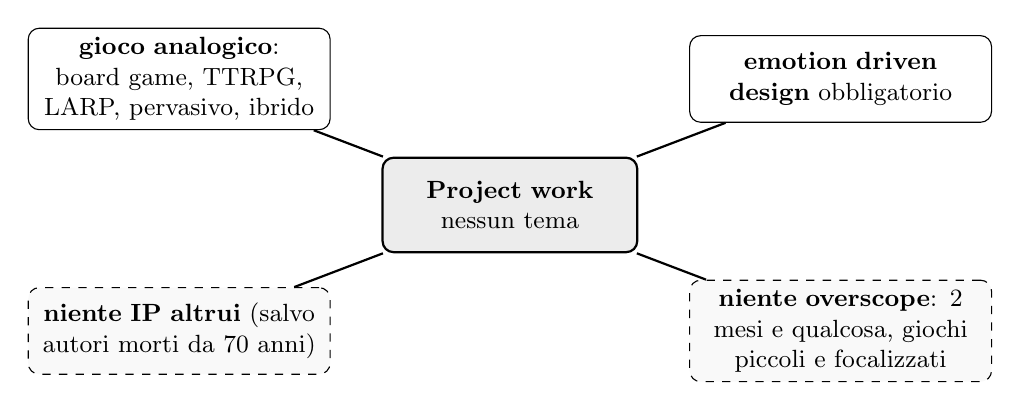
\begin{tikzpicture}[
    font=\small,
    centro/.style={draw, thick, rounded corners, fill=gray!15, text width=3.0cm,
      align=center, minimum height=1.2cm},
    vincolo/.style={draw, rounded corners, text width=3.6cm, align=center,
      minimum height=1.1cm, fill=white},
    no/.style={draw, dashed, rounded corners, text width=3.6cm, align=center,
      minimum height=1.1cm, fill=gray!5},
    linea/.style={thick}
  ]
  \node[centro] (c) at (0,0) {\textbf{Project work}\\ nessun tema};
  \node[vincolo] (a) at (-4.2,1.6) {\textbf{gioco analogico}: board game, TTRPG,
    LARP, pervasivo, ibrido};
  \node[vincolo] (b) at (4.2,1.6) {\textbf{emotion driven design}
    obbligatorio};
  \node[no] (d) at (-4.2,-1.6) {\textbf{niente IP altrui} (salvo autori morti da
    70 anni)};
  \node[no] (e) at (4.2,-1.6) {\textbf{niente overscope}: 2 mesi e qualcosa,
    giochi piccoli e focalizzati};
  \foreach \x in {a,b,d,e} { \draw[linea] (c) -- (\x); }
\end{tikzpicture}
\caption{Il \emph{mandate} del project work: due cose da fare (in alto) e due da
non fare (in basso, tratteggiate). Ricostruzione schematica della slide di
Daniele.}
\label{a7:fig:mandate}
\end{figure}

% ---------------------------------------------------------------------
\section{I gruppi}
\label{a7:sec:gruppi}

Poi i gruppi, tre gruppi da tre (tabella~\ref{a7:tab:gruppi}). La scelta è dei
docenti ed è ``insindacabile'', ma è basata sulle attività e sui task fatti
finora, ``sulla base di quello che vi abbiamo fatto fare negli ultimi giorni, come
lezioni, sulla vostra task e su quello che è stato un po' il nostro modo di
vedere''. Si è cercato di bilanciare anche gli \textbf{impegni di lavoro} di
ciascuno.

\begin{table}[htbp]
\centering
\begin{tabular}{@{}ll@{}}
\toprule
\textbf{Gruppo} & \textbf{Componenti} \\
\midrule
Gruppo 1 & Giordano, Nicola, Rita \\
Gruppo 2 & Gianmarco, Tancredi, Lorenzo Vergata \\
Gruppo 3 & Tiziana, Angelo, l'altro Lorenzo \\
\bottomrule
\end{tabular}
\caption{I gruppi del project work come li annuncia Daniele\protect\footnotemark.}
\label{a7:tab:gruppi}
\end{table}
\footnotetext{La trascrizione dice ``Giordano, Nicole, Rita, gruppo 2 Gianmarco,
Tancredi e Lorenzo V, gruppo 3 Tiziana, Angelo e Lorenzo''. ``Lorenzo V'' è Lorenzo
Vergata, come confermano poi i messaggi tra lui e Tancredi durante la pausa;
``Nicole'' è Nicola, a cui più tardi Beatrice dice che è nel gruppo ``con Giordano e
Rita''.}

Il progetto va sviluppato \textbf{durante il corso}: ``non vanno bene idee
pregresse, non portate nei vostri gruppi idee precedenti''. Le idee si sviluppano
insieme agli altri.

% ---------------------------------------------------------------------
\section{Le regole per lavorare in gruppo}
\label{a7:sec:regole}

Prima di lasciare la lezione a Beatrice, Daniele dà ``altri consigli per gli
acquisti''.

\paragraph{Rispettarsi.} ``La maggior parte del lavoro di un gruppo di sviluppo è di
\textbf{soft skill} più che di skill''. Bisogna capire come collaborare: se qualcuno
ha impegni di lavoro e fa fatica a garantire del tempo, ``partite da quello''. Non
si parte con ``un progetto grande come un castello disneyano'' per poi trovarsi
senza tempo; ci si dice invece ``io posso lavorare solo in questi momenti, lui o lei
solo in questi momenti'', e si cerca di fare ``qualcosa che abbia senso fare per il
tempo che abbiamo a disposizione''.

\paragraph{Taggare i docenti.} In caso di problemi si scrive ai docenti su
\textbf{Discord}, ma \textbf{taggandoli}: ``non lasciate messaggi senza taggarci,
se no li vedo una settimana dopo''. Oppure su \textbf{Telegram}.

\paragraph{Usare subito questi giorni.} Questi giorni vanno usati per il
\emph{brainstorming}: il tutoraggio con Ruggero è a breve (Daniele parla di ``48
ore'' per impostare il lavoro e capire che cosa fare).

\paragraph{Lavorare nel Drive.} Questa è una regola \textbf{obbligatoria}. Nel
Drive condiviso del corso ci sono le cartelle ``attività in classe'', ``dispense'',
``materiali didattici'' e ``project work''; dentro ``project work'' Daniele crea
tre cartelle, \textbf{gruppo 1}, \textbf{gruppo 2} e \textbf{gruppo 3}. Lavorare nel
Drive vuol dire evitare il più possibile di creare file fuori e caricarli dopo:
si aprono i Google Document lì e si lavora \textbf{in cloud}. Il motivo: se un
gruppo ha problemi e Daniele vuole aiutarlo, ha bisogno di vedere il
\textbf{processo mentale}, cioè che cosa è stato fatto nel documento, ``lo
\textbf{storico} del documento''. Un PDF o un \texttt{.docx} caricati così come
sono non hanno storico. Le cartelle vanno organizzate al meglio possibile; per
qualsiasi problema, ``basta chiedere''.

\paragraph{La dispensa sul brainstorming.} A seguito di questa lezione, ``tra stasera
e domani mattina'', Daniele registrerà una \textbf{dispensa}: il pezzo che venerdì
non c'è stato modo di fare, sul \emph{brainstorming} e sulla ricerca e sviluppo
``lato marketing'' e sugli strumenti di marketing nella ricerca e sviluppo. Metterà
a disposizione le slide e un video, con le slide del \textbf{brainstorming
strutturato}.

Nessuna domanda (``molti pollicioni, va bene''). Daniele ringrazia Bea ``per il
supporto e la condivisione'', saluta (``ci vediamo sicuramente il 12 di
ottobre'') e lascia la lezione.

% ---------------------------------------------------------------------
\section{Perché facciamo game design: due obiettivi}
\label{a7:sec:obiettivi}

``Ciao gruppo''. Beatrice comincia dando un po' di contesto: il corso è alla
\textbf{seconda edizione}, ci sono cambiamenti rispetto alla prima, e i docenti
stanno cercando di capire ``come rendervi il lavoro più agile e fattibile
possibile''. Nelle slide di oggi c'è molto, ``sarò onesta, credo troppo per la
lezione di oggi'', e quello che non si farà si riprenderà nella lezione successiva.
Il programma: ``mettere le mani in pasta'' per prepararsi ad affrontare un lavoro di
design; un po' di \emph{brainstorming} (da approfondire con i materiali di Daniele);
e una sorta di percorso di creazione di un gioco con un piccolo \textbf{esercizio di
design sprint}, a cui sarà dedicata la maggior parte della lezione. Alla fine del
corso i docenti chiederanno anche dei \textbf{feedback} su come è andato tutto.

Prima, però, un ``cappellino introduttivo'' sul \textbf{perché facciamo design}, già
anticipato nelle lezioni precedenti. Ci sono \textbf{due entità} che in questo
contesto si chiamano \textbf{obiettivi di design}:
\begin{enumerate}
  \item l'\textbf{obiettivo del gioco}, della produzione che si fa;
  \item l'\textbf{obiettivo personale} di chi progetta.
\end{enumerate}

\paragraph{L'obiettivo del gioco.} Un obiettivo di design del gioco, o del momento in
cui si sta facendo design, ha molte possibilità: raccontare un'esperienza di vita,
esplorare meccaniche o dinamiche, e così via; gli esempi della slide sono ``buttati
lì, sempre in brainstorming''. Si può decidere di fare un gioco per $N$ motivi, alcuni
personali e altri esterni al proprio bisogno personale.

Il punto è che \textbf{il motivo per cui affrontiamo la creazione di un gioco cambia
anche come progettiamo}. Beatrice vuole invitare la classe a ragionare su queste
cose, che spesso restano \textbf{ragionamenti interni} e invece è importante che
siano anche \textbf{condivisi}.

\paragraph{L'obiettivo personale.} L'obiettivo personale è semplice: rispondere alla
domanda \textbf{``perché sto facendo questo gioco?''}. Beatrice propone
\textbf{quattro categorie}, ``ma ce ne sono molte altre'', e probabilmente ne
emergeranno di nuove col crescere della disciplina; per la classe, i macro-obiettivi
saranno verosimilmente questi (figura~\ref{a7:fig:obiettivi}).
\begin{enumerate}
  \item \textbf{Voglio pubblicare un gioco.} Come gruppo di lavoro o come persona,
        voglio parlare a degli editori e pubblicare. Sotto questo cappello stanno sia
        la \textbf{pubblicazione con un editore} sia
        l'\textbf{auto\-pubblicazione}.
  \item \textbf{Voglio esprimere me stesso o me stessa.} È ``molto sottovalutato,
        troppo sottovalutato'': il gioco è uno strumento di espressione molto grande,
        che coinvolge anche altre persone. Magari non si vuole pubblicare né vendere,
        ma trasmettere davvero qualcosa che si è vissuto, qualcosa che si vuole
        raccontare; o si fa attivismo politico e si vuole un'attività che
        sensibilizzi sull'ecologia o su altri temi.
  \item \textbf{Voglio formare, informare o sensibilizzare.} Può sovrapporsi al
        punto precedente. Un gioco per insegnare meglio la matematica, per far
        conoscere un quartiere della propria città o un evento storico, per far
        crescere una competenza (aiutare le persone a parlare meglio in gruppo):
        ``$N$ situazioni di formazione''.
  \item \textbf{Voglio usare i giochi per il marketing e la comunicazione.} Portare
        l'attenzione su qualcosa: può essere un'espressione personale o una
        sensibilizzazione, ma anche un \textbf{prodotto} o un \textbf{servizio}. Lo si
        è visto con gli \emph{alternate reality game} del marketing, e in tante altre
        situazioni.
\end{enumerate}

\begin{figure}[htbp]
\centering
\begin{tikzpicture}[
    font=\small,
    domanda/.style={draw, thick, ellipse, fill=gray!15, text width=3.2cm,
      align=center, inner sep=2pt},
    ob/.style={draw, rounded corners, text width=3.3cm, align=center,
      minimum height=1.5cm, fill=white},
    freccia/.style={-{Stealth[length=2mm]}, thick}
  ]
  \node[domanda] (q) at (0,0) {\textbf{Perché sto facendo questo gioco?}};
  \node[ob] (p) at (-4.4,1.9) {\textbf{pubblicare}\\ con un editore o in
    autoproduzione};
  \node[ob] (e) at (4.4,1.9) {\textbf{esprimere me stesso/a}\\ raccontare,
    sperimentare, attivismo};
  \node[ob] (f) at (-4.4,-1.9) {\textbf{formare, informare, sensibilizzare}\\
    scuole, terzo settore, aziende};
  \node[ob] (m) at (4.4,-1.9) {\textbf{marketing e comunicazione}\\ prodotti,
    servizi, ARG};
  \foreach \x in {p,e,f,m} { \draw[freccia] (q) -- (\x); }
\end{tikzpicture}
\caption{Le quattro categorie di obiettivo personale proposte da Beatrice. ``Ce
ne sono molte altre''; esprimersi e sensibilizzare spesso si sovrappongono, e uno
stesso gioco può rispondere a più obiettivi.}
\label{a7:fig:obiettivi}
\end{figure}

% ---------------------------------------------------------------------
\section{Le competenze che ogni obiettivo richiede}
\label{a7:sec:competenze}

Ognuno di questi obiettivi personali richiede delle \textbf{competenze}, che ci si
fa ``in corso d'opera''. I docenti non si aspettano che gli studenti approfondiscano
ogni slide durante il corso, ma vogliono dire una cosa: se si crea un gioco, tutta
l'analisi di cui si è parlato (del mercato, delle persone, del target) va tenuta in
considerazione \textbf{in funzione dell'obiettivo}. Ogni obiettivo ha un modo
diverso di guardare il gioco e di produrlo. La slide mostra una ``carrellata'' di
competenze e conoscenze (tabella~\ref{a7:tab:competenze}).

\paragraph{Pubblicare con un editore.} Sono emerse domande anche dalla classe su come
capire che cosa sia meglio fare. Bisogna \textbf{conoscere il mondo della produzione}
di giochi da tavolo, di giochi di ruolo e di eventi ludici: chi esiste, che cosa fa,
a che prezzi mette fuori le cose, che tipo di prodotti vende già; se ci si riesce,
quante copie vengono vendute, quante persone comprano un biglietto. E
\textbf{conoscere le persone}: non solo ``c'è la casa editrice con il nome X'', ma
``all'interno ci lavorano X, Y, Z''. Partecipare agli eventi, mettersi in
connessione: sono tutte competenze, orientate a capire \textbf{come inserirsi} nelle
realtà che possono avere interesse a pubblicare.

\paragraph{Autoprodursi.} Le logiche sono diverse. Il mondo editoriale va conosciuto
comunque, perché in questo caso sono \textbf{competitor}; ma bisogna ragionare di più
verso il \textbf{pubblico}: capire come arrivare al momento in cui le persone
acquistano. Quindi parlare con gli utenti, affinare il marketing, analizzare i
competitor. E i competitor non sono solo quelli che fanno la stessa attività: per un
\textbf{evento dal vivo} un competitor può essere una fiera o un concerto, non per
forza un'attività di gioco; per un \textbf{gioco da tavolo formativo} un competitor
può essere un \textbf{corso}, non per forza un altro gioco. ``Immaginate i
competitor un po' più ad ampio spettro''. Infine, tutta una serie di informazioni
``non scontate'' e ``spesso prese sotto gamba'': \textbf{fiscalità e normative}.

\paragraph{Il GDPR: un'anticipazione.} Su questo, nella prossima lezione, Beatrice
farà ``un piccolo cappello'' sulle basi del \textbf{GDPR}, per poter raccogliere i
dati degli utenti e ricontattarli. È utile qualunque sia l'obiettivo: è sempre utile
avere, in una forma che permetta di risentirle, i dati delle persone con cui si è
venuti in contatto, che magari hanno testato il gioco, per tornare a scrivergli e
capire una serie di cose.

\paragraph{Esprimere se stessi.} Per sperimentare, per esplorare: qui ci sono
competenze ``spesso non raccontate, perché meno orientate al mercato'', che
riguardano \textbf{come trasmettiamo i contenuti} che vogliamo portare. È il lavoro
di \textbf{emotional design}, che ``sembra complicatissimo'', o comunque difficile da
definire; lo è, perché cambia per ogni gioco, ma col tempo si raffina sempre di più.
Chi vuole usare il gioco come sperimentazione personale, come linguaggio di dialogo
personale, deve capire bene quali sono i propri obiettivi: può essere ``voglio
comunicare la mia storia personale'', ma anche ``voglio trovare persone a me
affini'', o, ``banalmente'', ``voglio essere la persona che ha fatto il gioco più
conosciuto sulle \textbf{lumache da prato}''. Se è quello che si vuole raggiungere,
va bene: capito bene l'obiettivo, si capisce meglio tutto il resto, cioè
\textbf{che cosa voglio dire, a chi dirlo e perché} voglio dire determinate cose.

\paragraph{Formare, informare, sensibilizzare.} ``C'è un mondo'' su come si fa questo
design; qualcosa si vedrà nella prossima lezione, con le \textbf{escape room} e le
escape room formative. Per capire il mercato che può pagare queste attività, secondo
l'esperienza di Beatrice (``che non è onnisciente, ma è abbastanza puntuale al giorno
d'oggi''), le macro-voci in cui ci sono dei soldi, escludendo
l'\textbf{autofinanziamento} (che lei mette in una voce a sé), sono tre:
\begin{itemize}
  \item il \textbf{terzo settore} e i \textbf{bandi};
  \item il mondo delle \textbf{scuole} e della \textbf{formazione};
  \item la \textbf{formazione aziendale}: \emph{learning and development}, risorse
        umane e simili.
\end{itemize}
Sono tre mondi con logiche ``completamente diverse'' da quelle viste prima, e
Beatrice non ci si sofferma, perché non è il fulcro del corso. Ma già queste voci
bastano per sapere dove approfondire, se si vuole fare un gioco formativo: che cos'è
il terzo settore e che cosa significa proporgli dei giochi; che cosa sono i bandi
pubblici e quali enti li finanziano; e lo stesso per le scuole e per le aziende. E
poi c'è ``il magico mondo della \textbf{formazione finanziata}'', che sta sempre
sotto il cappello delle risorse umane: già googlando queste due parole si trovano
molte situazioni in cui si inserisce la proposta di giochi.

\paragraph{Il marketing.} Qui la parte principale da sapere è quella già vista
sull'\textbf{analisi del target} e sull'individuazione delle persone da coinvolgere.
Beatrice non si sofferma, perché secondo lei il marketing ``arriva dopo'': quando si
è progettato un po' di più (vale anche per la formazione) e si è sperimentato quello
che si è in grado di fare, allora si possono immaginare giochi per il marketing, che
sono giochi che portano l'utente a fare determinate cose. Per chi vuole approfondire,
la cosa principale è questa: si parla con delle \textbf{aziende}, e le aziende,
``anche le più virtuose'', hanno l'obiettivo di ``fare dei soldini''. Bisogna saper
rispondere alla domanda \textbf{``come aiuta l'azienda a fare più soldi?''}. I casi
sono due: \textbf{aumenta le vendite}, oppure fa aumentare \textbf{quanto l'azienda è
conosciuta}, o, se è conosciuta male, ne modifica in positivo la
\textbf{reputazione}. ``Non è un mondo bellissimo, ma è un mondo che esiste'': giochi
di questo tipo esistono tantissimo, e spesso non sono neanche raccontati come tali.
Beatrice lo dice perché magari si ha ``il gioco migliore del mondo'' e non si sa come
pagarsene lo sviluppo: questo può essere un modo.

\begin{table}[htbp]
\centering
\begin{tabular}{@{}p{3.0cm}p{9.6cm}@{}}
\toprule
\textbf{Obiettivo} & \textbf{Che cosa bisogna conoscere} \\
\midrule
Pubblicare con un editore & il mondo della produzione (chi c'è, che cosa fa, a che
prezzi, quanto vende); le persone dentro le case editrici; eventi e contatti \\
Autoprodursi & il mondo editoriale come competitor; il pubblico; marketing;
competitor ``ad ampio spettro'' (una fiera, un concerto, un corso); fiscalità e
normative; GDPR \\
Esprimere se stessi & come trasmettere i contenuti; \emph{emotional design}; che
cosa voglio dire, a chi e perché \\
Formare e sensibilizzare & terzo settore e bandi; scuole e formazione; formazione
aziendale (\emph{learning and development}, risorse umane); formazione finanziata \\
Marketing & analisi del target; ``come aiuta l'azienda a fare più soldi?'':
vendite, notorietà, reputazione \\
\bottomrule
\end{tabular}
\caption{Le competenze per obiettivo personale, ricostruite dalla carrellata di
Beatrice.}
\label{a7:tab:competenze}
\end{table}

\paragraph{Lo stesso gioco, più obiettivi.} Uno stesso gioco può rispondere a più
obiettivi. Si fa un gioco formativo, o un gioco per esprimersi, e si scopre che
potrebbe essere venduto a un'azienda, rispondere a un bando, entrare
perfettamente nel catalogo di un editore estero ``che non conoscevate fino a ieri'',
o di un editore italiano conosciuto in fiera. Quello che interessa a Beatrice è che
gli studenti abbiano chiari \textbf{gli interessi del mondo a cui parlano}, quando
hanno un gioco in progettazione o già fatto. Se si è consapevoli degli interessi
degli altri e del proprio obiettivo personale, ``diventa molto più facile il
dialogo''. Riuscire poi a vendere e ``imbroccare le cose giuste'' è un altro tema;
ma questi due elementi vanno avuti \textbf{prima}.

\paragraph{Approfondimento: il perché del designer.} Il tema dell'obiettivo personale
ha un parallelo in \emph{The Art of Game Design} di Jesse Schell, che apre il libro
non dal gioco ma dal designer stesso (``in the beginning, there is the designer''),
e più avanti dedica capitoli interi al rapporto con il \emph{cliente} e al
\emph{pitch}, cioè proprio al ``dialogo'' con gli interessi altrui di cui parla
Beatrice. Nella lezione, però, la distinzione tra
\emph{obiettivo del gioco} e \emph{obiettivo personale} ha soprattutto una funzione
pratica: è il primo argomento della chiacchierata iniziale del design sprint.

% ---------------------------------------------------------------------
\section{Il design sprint}
\label{a7:sec:sprint}

``Ora sono andata un po' veloce, e sono comunque lenta rispetto agli orari'':
Beatrice passa all'esercizio. Condivide un altro file (``che voi vedete bruttarello
qui e che poi vi caricherò''); chi non lo legge può mandarle ``un'emoji triste o
buffa''. Ha preparato \textbf{due moduli}; quello di adesso è su \textbf{come fare una
sessione di design sprint}.

\paragraph{Che cos'è.} Il design sprint si può usare per $N$ cose: ``dal decidere
come arredare casa a come risolvere il problema di non avere abbastanza soldi per
fare la spesa'', per qualunque problema. \textbf{Non è uno strumento nato per il game
design}: è nato per ragionare su problemi di progettazione e cercare soluzioni di
design. Beatrice lo ha \textbf{adattato all'uso sui giochi}, e lo ha diviso in
\textbf{fasi}, perché sono le fasi che invita i gruppi a provare a seguire. Il file
verrà caricato nella cartella condivisa degli strumenti. Oggi racconterà la prima
fase, ma la salterà, e si partirà dalla seconda.

\paragraph{Un invito, non un obbligo.} È ``uno strumento in più che vi dà una
direzione in caso la direzione non riusciate a trovarla in breve tempo''. Beatrice lo
dice apertamente: l'anno scorso alcuni gruppi hanno investito molto tempo in alcune
fasi della progettazione e non sono riusciti a concludere il gioco. Quest'anno si
vuole evitarlo, e per questo ci sono \textbf{due strumenti}: questo, e quello che si
vedrà alla fine di questa lezione e all'inizio della prossima, cioè tutte le voci che
compongono la progettazione di un gioco, per avere una \textbf{visione d'insieme} e
poter dire: ``abbiamo queste settimane prima del pitch e questi mesi prima della
consegna''. Ognuno ha un lavoro, una famiglia, dorme, mangia, fa cose che occupano
tempo: bisogna farsi ``dei conti pratici'', un tot di ore per una parte e un tot per
un'altra.

\paragraph{Il project management che non c'è.} Tutto questo fa parte del
\textbf{project management} di un progetto, e Beatrice avverte che nel mondo del
lavoro, ``nel gaming perlomeno'', \textbf{non esiste}: nella slide in cui sono state
presentate tutte le professioni non c'è un \emph{project manager} dei giochi, perché
le aziende sono ``ancora un po' in costruzione'' su questo lato; quelle italiane
almeno, mentre all'estero ci sono casi molto diversi, e nel videogioco funziona in un
altro modo. Questi strumenti vanno conosciuti per essere più consapevoli di
\textbf{come si funziona come persone}, preparandosi al fatto che il mondo esterno
non sempre segue logiche di organizzazione e ``più spesso bisogna un po' navigare le
onde''. Per il corso, però, sono molto utili: quando il gruppo ``per un attimo si
perde'', si può tornare a fare il punto con questi strumenti.

\subsection{Le fasi del file}
\label{a7:sec:fasi-file}

Beatrice scorre i ``titoloni'' del documento (figura~\ref{a7:fig:sprint}).
\begin{enumerate}
  \item \textbf{La chiacchierata iniziale}, che oggi si salta (si veda sotto).
  \item \textbf{Definire l'obiettivo di gruppo} del gioco: proposte e votazioni.
  \item Una piccola sessione di \textbf{ricerca e sviluppo} basata sull'obiettivo.
  \item Una prima sessione di \textbf{brainstorming} su quello che emerge, per
        rispondere all'obiettivo.
  \item La \textbf{valutazione} di tutto il brainstorming: che cosa si tiene e che
        cosa si butta, di tutte le idee uscite.
  \item Da lì in poi, l'\textbf{assegnazione dei ruoli}: chi fa cosa, con che tempi.
\end{enumerate}
Oggi si faranno le fasi dalla seconda in poi, fingendo che la classe sia un unico
grande gruppo di \textbf{nove persone} che inventa un gioco: ``faremo tutto quello
che serve per fare un brainstorming per avere il pitch del gioco''. Sarà un gioco
``del gruppo tutto'', quindi non lo si potrà portare a conclusione nel corso: serve
ad allenarsi con lo strumento.

\begin{figure}[htbp]
\centering
\begin{tikzpicture}[
    font=\small,
    fase/.style={draw, thick, rounded corners, text width=2.5cm, align=center,
      minimum height=1.3cm, fill=white},
    oggi/.style={fase, fill=gray!15},
    saltata/.style={fase, dashed, fill=gray!4},
    freccia/.style={-{Stealth[length=2mm]}, thick},
    nota/.style={font=\scriptsize\itshape, text width=2.5cm, align=center}
  ]
  \node[saltata] (f0) at (0,0) {chiacchierata iniziale (30 min)};
  \node[oggi, right=0.5cm of f0] (f1) {obiettivo del gioco: post-it e voto};
  \node[oggi, right=0.5cm of f1] (f2) {ricerca e sviluppo};
  \node[oggi, right=0.5cm of f2] (f3) {brainstorming su meccaniche, tipo,
    narrazione, setting};
  \node[oggi, below=1.1cm of f3] (f4) {voto, poi mappa impatto-sforzo};
  \node[oggi, left=0.5cm of f4] (f5) {percorso dell'utente};
  \node[fase, left=0.5cm of f5] (f6) {chi fa cosa, con che tempi};
  \node[fase, left=0.5cm of f6] (f7) {progettazione e sviluppo};
  \draw[freccia] (f0) -- (f1);
  \draw[freccia] (f1) -- (f2);
  \draw[freccia] (f2) -- (f3);
  \draw[freccia] (f3) -- (f4);
  \draw[freccia] (f4) -- (f5);
  \draw[freccia] (f5) -- (f6);
  \draw[freccia] (f6) -- (f7);
  \draw[freccia, dashed] (f7.north) -- node[midway, right=2pt,
    font=\scriptsize, align=left] {quando ci si perde:\\ di nuovo al voto}
    (f1.south west);
  \node[nota, above=0.1cm of f0] {saltata a lezione};
\end{tikzpicture}
\caption{Le fasi del design sprint adattato da Beatrice per il corso. In grigio le
fasi toccate a lezione (alcune solo raccontate per mancanza di tempo); la
chiacchierata iniziale è saltata. La freccia tratteggiata riassume il consiglio
``quando vi perdete, andate a votazione''. Ricostruzione schematica del file.}
\label{a7:fig:sprint}
\end{figure}

\paragraph{Una scaletta per il corso, non il design sprint.} Beatrice lo ripeterà più
avanti, a Nicola: la scaletta \textbf{non è una fase standard}, ``non voglio che vi
portiate a casa che il design sprint è tutto così, sempre, a queste fasi''. Prende
delle metodologie e le porta in una scaletta pensata per il corso.

\subsection{La chiacchierata iniziale}
\label{a7:sec:chiacchierata}

La prima fase è un \textbf{allineamento di gruppo}, e oggi si salta. Le domande:
\begin{itemize}
  \item quali sono i nostri \textbf{obiettivi personali} (quelli visti prima)?
        ``Magari il mio obiettivo in questo corso è provare a sperimentare. Oppure
        Lorenzo vuole fare un gioco per provare a venderlo da qualche parte, oppure
        io voglio fare un gioco per raccontare la storia della mia famiglia''.
        Allinearsi non vuol dire che sarà quello che si porterà a casa, ma che si
        conoscono i desiderata degli altri e c'è uno spazio per raccontare i propri;
  \item \textbf{che competenze ho}? A quali progetti ho già lavorato, e che cosa
        facevo in quei progetti?
  \item la ``domandona'': in questo corso voglio lavorare sulle \textbf{stesse
        competenze} su cui ho lavorato in passato, o ci sono attività che non ho
        ancora esplorato, che non ho mai fatto e vorrei esplorare qui? ``Non ho mai
        scritto testi, ma qua mi andrebbe di provare'', ``non ho mai fatto
        illustrazioni e qua mi andrebbe di vedere'': qui si può fare, e conviene
        capire in che ruolo mettere le proprie competenze. (Beatrice corregge anche
        un refuso nel file, in diretta.)
\end{itemize}
Per gruppi di tre persone, \textbf{30 minuti} bastano e avanzano: uno scambio in cui
``ognuno sa la situazione delle altre persone''. Beatrice invita a farla quando
inizierà il lavoro di gruppo.

\paragraph{Approfondimento: lo Sprint di Google Ventures.} Il \emph{design sprint}
nella forma più nota è quello descritto da Jake Knapp, con John Zeratsky e Braden
Kowitz, nel libro \emph{Sprint} (2016), nato a Google Ventures: cinque giorni per
passare da un problema a un prototipo testato con utenti reali, con passaggi molto
simili a quelli della lezione (mappare il problema, raccogliere ispirazioni,
proporre soluzioni individualmente e in silenzio, votare con adesivi a pallino,
decidere). L'adattamento di Beatrice ne conserva il cuore (lavoro individuale
silenzioso, presentazione, voto a pallini, tempi rigidi) ma lo piega ai tempi e agli
scopi di un corso: niente giornate intere, e la prima fase dedicata alle persone del
gruppo, non al problema.

% ---------------------------------------------------------------------
\section{La lavagna di Canva}
\label{a7:sec:canva}

``Ora vi condivido questa fantastica lavagna''. Per il \emph{brainstorming} ci sono
``tantissimi'' strumenti e modalità; oggi si usa il design sprint come modalità e una
\textbf{lavagna di Canva} come strumento.

\paragraph{Entrare.} Il link nella chat non è cliccabile, né si riesce a copiarlo
(``nemmeno copia e incolla''). Qualcuno lo copia a mano nella barra del browser e
riesce a entrare; un altro lo mette su Discord, dove ``funziona'', anche se a qualcuno
risulta che dal link di Discord non ha l'autorizzazione (``essendo che il link l'ho
copiato io, magari non ci sono i permessi''). Alla fine Beatrice crea un link
accorciato, ``più dettabile'' (\texttt{urli.it/31GRXQ}, secondo la trascrizione).

\paragraph{Gli strumenti in generale.} Canva è uno strumento per sessioni di
\emph{brainstorming} simile a molti altri; un altro è \textbf{Miro}, ``ma ce ne sono
davvero tanti''. Beatrice usa Canva perché è il più comodo per lei. L'impostazione
della lavagna \textbf{simula un incontro dal vivo}: le attività di oggi si possono
fare in digitale, a distanza, con uno strumento di questo tipo, oppure dal vivo con
\textbf{carta e penna}, un tavolo dove appoggiare i bigliettini, un muro dove
attaccare i post-it. ``Ve lo dico perché può essere utile anche per il futuro''.

\paragraph{Come si usa.} Beatrice ha ``loccato'' (bloccato) gli elementi della
lavagna, così che nessuno sposti per errore le cornici; si può selezionare e
zoomare liberamente (avvicinandosi le lavagne ``diventano più grandi''), ma bisogna
stare attenti a non cancellare il lavoro degli altri. Per cancellare: si seleziona
l'elemento e si preme il tasto di cancellazione, oppure il piccolo cestino nel menu
dell'elemento. Gli strumenti utili sono nel \textbf{menu a sinistra} di Canva, che ha
sette voci (Canva AI, Modelli, Elementi, Testo, Brand, Caricamenti,
\textbf{Strumenti}); sotto \textbf{Strumenti} (l'icona con una ``pennina'') ci sono,
tra gli altri, il \textbf{testo} e i \textbf{foglietti adesivi}: ``veri e propri
post-it, come quelli che usereste dal vivo''. Si sceglie un colore, il post-it compare,
lo si ingrandisce o rimpicciolisce e ci si scrive sopra.

\paragraph{Le prove.} La prova serve anche ad allinearsi sullo strumento, ed è
movimentata. I post-it compaiono uno dopo l'altro (``Giordano, anche Lorenzo'',
``vedo una C'', ``Rita sta scrivendo''); Gianmarco entra senza il suo account e
compare come ``Leone Marino'', uno dei nomi di animale che lo strumento assegna
agli utenti anonimi\footnote{La trascrizione dice ``è come l'anonimo di Giuseppe'':
con ogni probabilità il riferimento è agli ``animali anonimi'' con cui Google e
altri servizi mostrano chi partecipa senza account.}. Si scopre che se la
lavagna di base è bloccata non si riesce a scrivere nei post-it (``io l'ho imparato
adesso, perché credevo non funzionasse così''), e Beatrice sblocca. Qualcuno sposta
per sbaglio l'intera cornice (``oh mio Dio, sono uscito, e qualcuno ha spostato tutta
la lavagna''), qualcuno ha post-it finiti fuori dalla lavagna o giganteschi, una
studentessa (``una grafica fissata con l'impaginazione'') prova a riallineare
tutto. Angelo, che è collegato \textbf{dal cellulare}, non riesce a trascinare il
post-it (``non me lo fa trascinare''); Beatrice lo guida passo per passo e alla fine
decide di creargli lei dei post-it con il proprio nome sopra, che Angelo userà
(``ci ricorderemo che i tuoi post-it sono quelli con il nome di Beatrice''), anche
se poco dopo Angelo riesce a crearne uno da solo (``ce l'ho fatta'').
``Dal telefono è anche più complicato, è normalissimo''. Beatrice avverte che
\textbf{Miro è un po' più intuitivo} di Canva, e che servirà molto spazio: il gioco di
fare le cose piccole e zoomare sarà utile soprattutto nella ricerca e sviluppo.

\paragraph{Lo strumento conta il giusto.} ``Di tutto questo, lo strumento ci interessa
il giusto'': si può usare Miro, si possono scrivere le cose a mano. \textbf{Ci
interessa il procedimento}.

% ---------------------------------------------------------------------
\section{Prima fase: che obiettivo vorrei dare a questo gioco?}
\label{a7:sec:fase1}

La domanda della prima fase è \textbf{``che obiettivo vorrei dare a questo
gioco?''}. Le regole:
\begin{itemize}
  \item ognuno scrive \textbf{al massimo tre risposte}, e almeno una;
  \item \textbf{una risposta per post-it};
  \item non è il genere del gioco e non sono le meccaniche: è ``più a volo
        d'aquila'', quello che si vorrebbe che il gioco ottenesse; può riguardare
        anche le \textbf{emozioni}, cioè che cosa far provare alla persona che gioca.
\end{itemize}
Gli esempi del file mescolano apposta livelli diversi: ``un gioco formativo per
insegnare l'inglese'', ``un gioco con dei pinguini blu'', ``un GDR per sensibilizzare
sulla lotta di classe'', ``un gioco fantasy sulla vendetta'', ``un gioco con delle
pedine gigantesche'', ``un gioco che faccia esplorare un quartiere''.

\paragraph{I timer.} E qui la cosa da ricordare di tutto il procedimento:
\textbf{mettere i timer}. Nei processi creativi di gruppo, e probabilmente lo si è già
visto succedere, ci si fa prendere da quello che sta avvenendo, dai dialoghi, dalle
idee che emergono. Beatrice richiama la lezione precedente su \textbf{divergenza e
convergenza}: c'è un momento in cui si apre, si esplora, si buttano idee; ma ``a un
certo punto bisogna \textbf{quagliare}''. Darsi un tempo di orologio dice fino a
quando si esplora; quando suona il timer, bisogna riportare in ordine la situazione.
``È la cosa importante di tutto il processo: dare dei tempi e provare a
rispettarli''. Il primo timer è di \textbf{5 minuti} (``dai 5 ai 10'').

\paragraph{Gianmarco arriva.} Gianmarco, ``arrivato un po' in corsa'', chiede il
contesto: si può buttare qualsiasi idea? È un esercizio, risponde Beatrice, per
imparare a fare \emph{brainstorming} e poi mettere in ordine le idee: ``vai pure
libero''.

\paragraph{La parola proibita.} Mentre scrivono, Rita avverte i compagni: qualcuno
ha scritto \emph{divertire} su un post-it, e ``dovremmo evitare di usare questo
verbo''\footnote{Il riferimento è alla regola, ricorrente nel corso, per cui ``far
divertire'' non è un obiettivo di design: è troppo generico per orientare le
scelte.}, ``conviene modificarlo prima che lo veda qualcuno'' (Ruggero, si
capisce). Beatrice: ``Io non dirò niente, però è un ottimo consiglio''. Del resto,
aggiunge, sono idee che non verranno condivise con gli altri docenti: è un esercizio
per imparare la procedura, che non è neanche detto si userà esattamente così. Le idee
di oggi possono avere vita propria e crescere, ``ma non in questo corso'': i gruppi
del progetto partiranno da zero.

% ---------------------------------------------------------------------
\section{Il racconto delle idee}
\label{a7:sec:racconto}

Prima della votazione, che Beatrice anticipa (si veda la
sezione~\ref{a7:sec:votazione}), \textbf{ognuno racconta che cosa ha scritto} e dice
\textbf{dove sono} i suoi post-it, così che tutti possano trovarli sulla lavagna. In
questa fase valgono due regole:
\begin{itemize}
  \item le altre persone possono fare \textbf{solo domande}: chiarimenti su che cosa
        si intende, su perché è emersa un'idea; ``tutte le domande che vi vengono in
        mente vanno benissimo'', anzi Beatrice invita a farle, perché ``c'è ancora
        tanto che può uscire'';
  \item \textbf{niente commenti}, ``né nient'altro''. Se non si hanno domande, non si
        dice nulla.
\end{itemize}
E Beatrice si fa da parte: ``fate finta che io non esista''. Ricorderà solo di dire
dove sono i post-it; il gruppo deve autogestirsi, come in un vero lavoro di gruppo
in cui nessuno dà la direzione. Poi si accorge di aver dimenticato il timer anche
qui: tutte le idee vanno raccontate in circa \textbf{15 minuti}, ``tenetene conto
quando fate le domande, quando rispondete, quando raccontate''.

\subsection{Rita}
\label{a7:sec:idee-rita}

Rita (post-it arancione, rosso e giallo, sovrapposti nell'angolo in alto a sinistra)
ha scritto tre idee.
\begin{description}
  \item[Un gioco educativo.] Si è avvicinata a questo mondo con l'idea di dare
        qualcosa in più alle nuove generazioni: è quello che l'ha spinta a diventare
        game designer.
  \item[Un gioco che costringe le persone a collaborare.] Quando la collaborazione è
        necessaria per raggiungere un obiettivo, bisogna affrontare problemi con se
        stessi e con gli altri, e questo è costruttivo e stimolante per tutti. È anche
        il suo approccio alla vita: ``condividere, collaborare per imparare''.
  \item[Un gioco sull'arte.] È la sua più grande passione: avvicinare le persone a
        un'arte ``non proiettata verso l'IA''.
\end{description}
Le domande. Il gioco sull'arte è sulla storia dell'arte, i grandi pittori, o un gioco
in cui \textbf{le persone fanno gli artisti}? La seconda: avvicinarle alla disciplina
in maniera attiva; e in effetti, osserva Rita, potrebbe rientrare nel gioco educativo,
con le scuole. Il gioco educativo, per che età e in che contesto? Non ci ha ancora
pensato nello specifico, ma pensava a bambini che stanno crescendo, elementari e
medie: per gli adolescenti ci vuole qualcosa di più attivo e stimolante a livello
emotivo, forse un LARP. Poi chiede lei un parere a una compagna con esperienza di
questi giochi: ci sono fasce d'età più interessate a certi tipi di gioco?
``Dipende'', risponde la compagna: si sente il gruppo, e se il gioco è educativo lo
si orienta anche, per esempio decidendo se farlo competitivo o no. A lei è sempre
piaciuto \textbf{mescolare competizione e collaborazione}: le \textbf{cacce al
tesoro} sono notoriamente competitive, ma le sue richiedevano sempre una
collaborazione tra i gruppi, e alla fine \textbf{il tesoro era per tutti}: c'era la
soddisfazione di chi era arrivato primo, ma il premio era di tutti. ``Bello, e
stimolante, perché si deve collaborare per raggiungere un obiettivo''.

\subsection{Nicola arriva}
\label{a7:sec:nicola}

A questo punto entra Nicola. Beatrice gli spiega in breve che cosa sta succedendo:
un esercizio di design sprint, ``una metodologia, anzi varie metodologie che
riguardano tante forme di design, non solo quello dei giochi'', per avere una
direzione quando un gruppo si perde o non sa come allinearsi; la prima fase è
rispondere a ``che obiettivo vogliamo dare al gioco''; i compagni hanno dato tre
idee ciascuno, che ora si leggono e poi si votano. E gli dice il suo gruppo: ``sei nel
gruppo 1, con Giordano e Rita'', ``non per motivi'', lo rivedrà nelle slide che
Daniele caricherà. Nicola entra nella lavagna come ``Nick''.

Poco dopo, Nicola chiede ``un quick check-up'': si sente ``in alto mare'', ``una
zavorra''. I post-it sono già divisi in gruppi? Sono concept di personaggio o di
gioco, di ogni singola persona? Si stanno comparando? Beatrice riconosce di non
essersi spiegata abbastanza e rispiega: si sta \textbf{testando la metodologia},
fingendo di essere un unico gruppo di nove da cui deve uscire ``una bozza di gioco'';
la scaletta non è standard ma costruita per il corso; per decidere l'obiettivo del
gioco ognuno butta giù idee in silenzio sui post-it, poi le si leggono (``una fase di
brainstorming aperto'') e infine le si vota.

Nicola chiede com'è il voto: qualitativo o quantitativo? Si vota sulla quantità di
contenuto, sulla tipologia, ``un voto vale più di un altro''? Nessun voto vale più di
un altro, risponde Beatrice: ognuno avrà \textbf{sei voti}, ``immagina di avere sei
pallini adesivi'', e può metterli anche tutti sulla stessa idea. A Nicola lo schema
ricorda quello studiato in \textbf{organizzazione aziendale}, quando si avvia un
progetto; Beatrice conferma che il design sprint si usa in moltissimi contesti, ``molto
sulle soluzioni da proporre'', anche in sociologia. Nicola chiede ancora se c'è stata
una spiegazione prima del lavoro: c'è stata una piccola introduzione sui motivi per cui
si fa design (recuperabile dalle slide o dalla registrazione), e poi ci si è buttati
sulla domanda. Infine: ci sono linee guida, ``o siamo randomici''? ``Per ora è tutto
libero, rimaniamo leggerissimi''. Nicola si scusa con la classe per il tempo rubato.

\subsection{Lorenzo Vergata}
\label{a7:sec:idee-vergata}

Lorenzo Vergata (post-it sopra quelli di Rita) presenta tre idee, mentre ``qualcuno
ha mosso la lavagna'' e per un momento ``è scomparso tutto''.
\begin{description}
  \item[I funghi.] \textbf{Esplorazione del bosco per sensibilizzare sulle specie
        fungine e sul rispetto della natura}, ``semplicemente perché siamo in periodo
        di funghi'': la prima cosa che gli è venuta in mente.
  \item[Frenetismo.] Partite rapide, ``quasi caotiche dall'esterno, ma
        pseudo-organizzate dall'interno fra i giocatori''. Si è chiesto che cosa cerca,
        a 26 anni, in un gioco: non partite lunghe, ma frenesia. Frenesia, quindi,
        ``per gente neolaureata e simile''.
  \item[Paura.] Nascondino; fuggire da qualcuno all'aperto, senza luci; o in casa,
        staccando la corrente all'inizio del gioco. ``Il gioco deve far paura'':
        senza aver fatto ricerca, pensa che non ci siano molti giochi che sfruttano la
        paura dei giocatori come dinamica.
\end{description}
Le domande, e qualche commento che sfugge alla regola. L'idea della paura è pensata
come un \textbf{LARP}, all'esterno, o come un gioco da tavolo? Lorenzo pensa che il
modo più semplice di creare paura sia un LARP, ma ``nulla toglie'' di farlo da tavolo,
studiando come un gioco da tavolo possa incutere timore. Una compagna osserva che la
paura si definisce in tanti modi: \textbf{pressione}, \textbf{ansia} (più facili da
tavolo) e \textbf{jumpscare} (più da LARP); bisognerebbe dare una dimensione al
concetto, ma è ``una bella sfida''. Le ricorda quando da ragazzina giocava a
\textbf{guardie e ladri} al mare, di notte, nelle case degli amici: si creava un
clima di paura e tensione, anche perché ci si facevano gli scherzi.

Un altro studente, che gioca ``per la maggior parte del tempo'' a giochi di ruolo da
tavolo\footnote{Dal contesto, con ogni probabilità Nicola, che poco dopo si presenta
come ``un grande giocatore di TTRPG''.}, conferma che la paura è ``un fantastico
strumento'', ma pone un problema: se diventa un \textbf{gioco pervasivo}, c'è un
\textbf{danno collaterale}, cioè \textbf{spaventare chi non gioca}. ``Immagino una
persona che corre a mezzanotte in giro per Roma urlando di paura'': terrificante per
chi la vede, e si coinvolgono persone che non vorrebbero provare quella paura.
Lorenzo concorda: bisognerebbe tarare, andando più verso quello che diceva la
compagna, cioè il momento in cui sei nascosto e senti che chi ti cerca è ``letteralmente
a fianco a te'', e ti pervadono paura e ansia. Ma ``basta poco'' per tirare in mezzo
estranei: chi vede una persona che ne insegue un'altra che cerca di nascondersi
``chiama la polizia al minuto zero''. Se sono bambini di sei anni, ``stanno
giocando''; se vedi un ventenne, ``che cosa sta accadendo?''.

Infine l'esplorazione del bosco: come sarebbe, come gioco? Una guida che ti porta nel
bosco? ``Fatta sul posto è tosta'': sarebbe semplicemente una gita con un
\textbf{micologo}. Ma \textbf{da tavolo} si potrebbe fare. Sul fronte della natura si
possono inserire meccaniche che \textbf{simulano il comportamento dei funghi}: sotto
di loro c'è il \textbf{micelio}, che fa da rete di comunicazione tra le piante, e ne
potrebbe uscire un gioco ``pseudostrategico''. Sulla \textbf{commestibilità} si può
immaginare uno scontro carta contro carta, una specie di sasso-carta-forbice: ``il
fungo buono te lo annullo con questo cattivo'', mentre certi funghi che ``sembrano
buoni'' rovinano tutto il raccolto, cioè una sola carta può rovinare molte carte di
funghi buoni. ``Potrebbe anche essere frenetico, chissà''.

\subsection{Tancredi}
\label{a7:sec:idee-tancredi}

Tancredi ha scritto in modo ``molto più riassunto''.
\begin{description}
  \item[Un gioco cooperativo.] È ``un grande fan dei cooperativi'', anche piccoli,
        come \emph{Hanabi}\footnote{La trascrizione dice ``Anabis''.}, \emph{Sky Team},
        \emph{Quicksand}: gli piace molto la meccanica della cooperazione.
  \item[Un gioco per il terzo settore.] Riprende la categoria vista prima, ma senza
        grandi idee: per questo tipo di gioco sarebbe importante capire \textbf{per chi}
        lo si fa, e non sa quanto sia realizzabile nel loro caso.
  \item[Un GDR.] Non conosce praticamente per niente i giochi di ruolo, li ha
        scoperti in queste lezioni: ``perché no?'', provare a sperimentare quel
        settore.
\end{description}
Che cosa aveva immaginato per il terzo settore? Secondo Tancredi un modo sarebbe
cercare delle realtà, anche solo su internet, sui loro siti, e capire che cosa
potrebbe essere interessante per loro, ``anche se poi non glielo si propone
veramente, perché questa è un'esercitazione''; con l'obiettivo di dare una mano,
diffondere quello che fanno. Un compagno racconta (più un commento che una domanda)
di aver giocato \emph{Nemesis: Retaliation} dal vivo nella modalità semicooperativa,
con i traditori, e ora online su \textbf{Board Game Arena}\footnote{La trascrizione
scrive ``BGA'', la sigla abituale del sito.} con più o meno gli stessi amici, in
modalità cooperativa, usando la chat: ``stratosferico, così mi diverto''. Se invece
``a un certo punto uno ti dà una ginocchiata sui denti''\ldots{} Tancredi: in
associazione ``quasi mai nessuno vuole fare cooperativi'', e lui è sempre lì; gli
piacciono anche i competitivi, ma certi giochi ``vale la pena giocarli così''.

\subsection{Tiziana}
\label{a7:sec:idee-tiziana}

Tiziana (post-it sotto quelli di Tancredi) ha scritto tre idee.
\begin{description}
  \item[Un board game, di costruzione, gestionale ambientato.] Le piacerebbe fare
        esperienza di costruzione di un gioco da tavolo e non saprebbe da che parte
        cominciare (come Tancredi con i giochi di ruolo: ``non ho idea, quindi mi
        piacerebbe provare''). Un \textbf{gestionale} perché le piace l'aspetto
        gestionale, ma \textbf{ambientato}, ``non so se è una chimera''.
  \item[Un'escape room per far divertire.] ``Lo so che non devo usare divertire, ma
        non sono riuscita a trovare nessun'altra cosa'', e soprattutto far divertire
        lei mentre la costruisce. E far nascere la \textbf{collaborazione}. Dal vivo o
        da tavolo, entrambi vanno bene; il tema non lo sa. Le piacciono gli
        \textbf{indovinelli}, trovare soluzioni; ma vorrebbe enigmi \textbf{misti}, non
        tutti dello stesso tipo, perché quando sono tutti uguali diventano ``o troppo
        cervellotici o ripetitivi''.
  \item[Un gioco interattivo per far conoscere la città.] Una parte di essa, perché
        Roma ``è abbastanza gigantesca''; l'aveva immaginato coinvolgendo perfino i
        \textbf{passanti}, ``ma non so se sia fattibile''.
\end{description}
Tancredi chiede: quando parli di gestionale, hai un riferimento? Un gioco economico,
con competizione e interazione molto alte, o qualcosa di meno interattivo,
``più German''? Tiziana non lo sa: da giocatrice è più ``mi coltivo il mio orticello''
(gli economici interattivi ``non sono i miei preferiti''), ma potrebbe essere anche
interattivo: intendeva la \textbf{gestione delle risorse} in generale. La cosa
fondamentale è che sia ambientato, ``che senti di essere in quel posto''. Un
compagno le suggerisce \emph{Akropolis}, per l'ambientazione e per l'idea di
costruire la propria città con tessere di tre esagoni sovrapposte, in cui i colori che
restano in cima diventano i quartieri: un approccio per non renderlo ``troppo
gestionale German'', magari con una città costruita tutti insieme. Tiziana non lo
conosce. Beatrice interviene: si possono fare domande, ``ma non altre cose'',
altrimenti si usa troppo tempo; e manca un minuto. Tancredi: ``domanda sbagliata,
scusate''. ``Va tutto bene, siamo qui apposta per capire le dinamiche''.

\paragraph{Il timer che scade.} Manca un minuto e mancano ancora cinque persone.
Beatrice concede \textbf{altri dieci minuti}, ``ma dentro questi dieci minuti dovete
starci'': alla fine si passa allo step successivo, ``quello che è stato detto è stato
detto''. Qualcuno propone due minuti a testa; ``se volete, sì, però non posso
dirvelo io'': serve ad allenare il gruppo.

\subsection{Angelo}
\label{a7:sec:idee-angelo}

Angelo, colto un po' di sorpresa (``ci ho messo un'eternità a scriverlo, abbiate
pazienza''), ha i post-it in basso a sinistra.
\begin{description}
  \item[Un gioco di ruolo basato su un'app.] Così che la \textbf{mappa} possa essere
        continuamente aggiornata.
  \item[Un board game con possibili espansioni.] Qualcosa ``tipo \emph{Magic}, ma non
        per forza così evoluto'': ogni tanto si aggiungono carte che modificano la
        strategia.
\end{description}
Il tema è variabile, ma più fantasy o fantascienza che realismo; non aveva pensato a
un'emozione particolare. Qualcuno trova interessante il board game ``aggiornabile''.
E che cosa intende per mondo condiviso? Qualcosa come i giochi online divisi per zone
(Europa dell'Est, Europa dell'Ovest), ma molto più ristretto: si parte con
un'avventura in un \emph{medieval fantasy}, e qualcuno nella tua zona pensa a un'isola
con ambientazione \emph{steampunk} e la aggiunge al mondo, così che altri possano
andarci e ``ruolare'' in un mondo steampunk. ``Una sorta di \emph{sandbox}'':
ognuno parte dal suo stile e ci si trova in posti sempre diversi, senza un paesaggio
ripetitivo.

\subsection{Gianmarco}
\label{a7:sec:idee-gianmarco}

Gianmarco (in basso a destra) presenta tre idee.
\begin{description}
  \item[Un gioco da tavolo per bambini dai 6 agli 8 anni.] Che li spinga a
        \textbf{raccontare}, incentrato su \textbf{esplorazione e scoperta}: è la fase in
        cui i bambini iniziano a staccarsi un po' dai genitori, e nell'esplorare provano
        ``quel misto di curiosità e paura''. Con elementi grafici, un po' di
        casualità; una parte di sistema per sviluppare la \textbf{logica} e una parte di
        immagini per l'\textbf{immaginazione}.
  \item[Un board game narrativo sulla guerra.] Con le meccaniche di \emph{Mage
        Knight}\footnote{La trascrizione dice ``Image Night'' e ``Mage Night''.}:
        ``l'ho veramente buttato a caso, è una cosa senza senso''.
  \item[Un'escape room basata sul tempo.] Si deve uscire dall'ufficio, ma il tempo
        non scorre mai: bisogna risolvere enigmi per far scattare \textbf{le 17} e
        uscire finalmente.
\end{description}
Un compagno ricorda una scena dei \emph{Simpson} in cui Bart guarda continuamente
l'orologio della classe, che a un certo punto torna indietro; e suggerisce una
meccanica del tempo non in tempo reale ma a eventi, ``cose che si innescano dopo tot
minuti'' (``so che tra tre minuti mi bolle l'acqua e succede qualcosa''). Un altro
nota che è bella ``la cosa al rovescio'': di solito il timer si accorcia e ti
esaurisce, qui devi farlo andare avanti. Qualcuno trova curiosa l'idea centrale e
chiede perché le meccaniche di \emph{Mage Knight} dovrebbero rappresentare l'orrore
della guerra. Il motivo è semplice: è un periodo di guerra, a Gianmarco piace
\emph{Mage Knight} e gli piacciono i board game narrativi, ``ho messo tutto insieme,
ho fatto un po' un pastiche''.

\subsection{Nicola}
\label{a7:sec:idee-nicola}

Mancano tre minuti e mezzo per tre persone: ``un minuto a testa''. Nicola va
``rapidissimo''.
\begin{description}
  \item[Un gioco di ruolo sui tempi morti: la cucina.] È un grande giocatore di
        TTRPG, e ha notato che i giochi di ruolo da tavolo hanno regole ben stabilite
        ma quasi nessuno ha meccaniche sui \textbf{tempi morti}: in un fantasy alla
        \emph{D\&D}, quando ci si accampa ``è sempre molto randomico''. Gli
        interesserebbe un GDR basato sulla \textbf{cucina}: restare sazi per andare
        avanti nelle missioni, arrangiarsi con quello che si trova; ispirandosi a
        \emph{Dungeon Food}\footnote{Così nella trascrizione. Si tratta con ogni
        probabilità di \emph{Dungeon Meshi} (in italiano \emph{Dungeon Food}),
        manga e anime in cui gli avventurieri cucinano e mangiano i mostri del
        dungeon.}, dove si mangiano i mostri per andare avanti, perché non sempre si
        hanno le provviste.
  \item[Un gioco strategico con bluff e ruoli nascosti.] Da giocatore di ruolo, perché
        non provare uno strategico da tavolo? Lo baserebbe sulla deduzione, sul
        \textbf{bluff} e sui \textbf{ruoli nascosti}. Su una gigantesca plancia ognuno
        parte senza nazione e, ispirandosi al videogioco strategico \emph{Humankind},
        ne sblocca: Roma, che vince \textbf{conquistando}, e allora la tua strategia
        diventa conquistare; più avanti gli Egizi, che vincono \textbf{costruendo
        opere}. L'obiettivo è non far capire \textbf{in che modo vuoi vincere}: quale
        nazione, o quale somma di nazioni, sei, e quali sono i tuoi metodi di vittoria.
  \item[Un LARP sul cambiamento visibile dei personaggi.] Non ne sa niente, ma gli
        interessa: persone vestite di bianco, ``come dei camici bianchi'', senza
        emozioni. Chi si sporca di \textbf{rosso} diventa più nervoso, rabbioso,
        isterico; di \textbf{blu}, più triste; di rosso e blu, arrabbiato e triste;
        di \textbf{verde}, prova anche disgusto. Una \textbf{somma di emozioni}, con
        obiettivi che costringono a sporcarsi: ``devi prendere la chiave segreta dentro
        il secchio rosso; ora hai la mano e mezza manica sporche di rosso, sei anche
        rabbioso''.
\end{description}

\subsection{L'altro Lorenzo}
\label{a7:sec:idee-lorenzo}

L'altro Lorenzo non è sicuro di aver seguito bene l'obiettivo: forse è stato
``troppo personale, troppo generico''. Ha scritto: \textbf{esprimere me stesso};
\textbf{raccontare il mio mondo fantasy attraverso un GDR}; \textbf{esplorare
tipologie di gioco nuove}, almeno per lui, come l'escape room o il LARP. Non ha in
mente cose specifiche. Qualcuno gli chiede se ne aveva in mente parlando del suo
gioco: sì, ma era un pensiero personale, e in un lavoro di gruppo ``non è che si può
imporre per forza il proprio mondo scritto''.

\subsection{Giordano}
\label{a7:sec:idee-giordano}

Il timer è scaduto, ma Beatrice concede a Giordano, l'ultimo, una breve presentazione
(all'inizio non si sente). Giordano non ha puntato su un gioco specifico ma su
\textbf{aspetti da inserire} in un gioco. Il primo è l'\textbf{accessibilità}: ``non
vorrei che qualcuno potesse mai dire \emph{non posso giocare a questo gioco}; al
massimo, \emph{non mi interessa}''. Il secondo è la \textbf{creatività}: di chi gioca,
precisa a una domanda, non di chi progetta.

\begin{table}[htbp]
\centering
\small
\begin{tabular}{@{}p{2.3cm}p{10.4cm}@{}}
\toprule
\textbf{Chi} & \textbf{Le idee sui post-it} \\
\midrule
Rita & gioco educativo (elementari e medie); gioco che costringe a collaborare;
gioco sull'arte, in cui si fa gli artisti \\
Lorenzo Vergata & esplorazione del bosco per sensibilizzare sulle specie fungine e
sul rispetto della natura; frenesia (partite rapide, caotiche fuori e organizzate
dentro); paura (nascondino, fuga al buio) \\
Tancredi & gioco cooperativo; gioco per il terzo settore; GDR \\
Tiziana & board game gestionale ambientato; escape room con enigmi misti e
collaborazione; gioco interattivo per far conoscere una parte di Roma \\
Angelo & GDR con app e mappa condivisa aggiornabile; board game con espansioni che
cambiano la strategia \\
Gianmarco & gioco per bambini di 6--8 anni su esplorazione e scoperta; board game
narrativo sulla guerra con le meccaniche di \emph{Mage Knight}; escape room in cui
bisogna far arrivare le 17 \\
Nicola & GDR sulla cucina e i tempi morti; strategico con bluff e nazioni nascoste;
LARP delle emozioni a colori \\
l'altro Lorenzo & esprimere se stesso; il proprio mondo fantasy in un GDR; esplorare
escape room e LARP \\
Giordano & accessibilità; creatività di chi gioca \\
\bottomrule
\end{tabular}
\caption{Le idee della prima fase dell'esercizio, persona per persona.}
\label{a7:tab:idee}
\end{table}

% ---------------------------------------------------------------------
\section{La votazione a pallini}
\label{a7:sec:votazione}

Beatrice blocca la lavagna (i post-it non si possono più spostare, ma ci si può
scrivere sopra), allarga un po' lo spazio dei post-it di Rita, e spiega prima
l'attività in sé, poi come farla su Canva.

\paragraph{Le regole.} Ognuno ha \textbf{sei pallini}: ``immaginatevi proprio di avere
dei pallini adesivi''.
\begin{itemize}
  \item Si mettono sulle idee che piacciono di più, cioè quelle \textbf{che si
        vorrebbero produrre}, su cui si vorrebbe lavorare.
  \item Si possono mettere \textbf{più pallini sulla stessa idea}, anche tutti e sei.
  \item Si può \textbf{votare la propria idea}.
  \item \textbf{Non si deve spiegare} perché si vota.
  \item Si devono \textbf{usare tutti e sei}: non si può non votare o metterne meno.
\end{itemize}
Alla fine restano solo i post-it con più pallini. Se uno ne ha più degli altri, è
l'idea su cui si lavora; se ce ne sono due o tre in testa, \textbf{si rivota} tra
quelli.

\paragraph{Su Canva.} Beatrice propone, ``brainstormando sempre, quindi non so se è
l'idea migliore'', di usare i \textbf{pennarelli} di Canva (ancora in Strumenti),
ognuno con un colore. Seguono le prove fuori dalla lavagna (Beatrice disegna ``un
cuore gigantesco viola'') e un lungo appello dei colori, complicato dal fatto che il
colore del cursore di qualcuno non coincide con quello del suo pennarello e che
compaiono più ``soli'' disegnati per prova\footnote{L'assegnazione dei colori, per
quanto ricostruibile: Giordano arancione, Nicola verde chiaro, Lorenzo Vergata ``blu
pastello'', Tancredi blu, Gianmarco viola scuro, l'altro Lorenzo rosso, Tiziana nero,
Angelo azzurro (assegnato da Beatrice), e una studentessa, probabilmente Rita, un
giallino ``che forse non si nota''. Per i colori poco visibili Beatrice suggerisce
pallini grossi accanto al post-it.}. Nessuno è ``morto'' finora (``vivi, vive''), e
dopo la votazione ci sarà una pausa. Timer di \textbf{5 minuti}.

\paragraph{Il timer di Canva.} Durante il voto Rita scopre che Canva ha un
\textbf{timer integrato}, in basso, e lo attiva (``timer gigante''): da qui in poi lo
si usa. ``Questa è una cosa che era molto utile'', dice Beatrice: aveva provato a
metterlo in altre forme. Chi ha finito i pallini mette il mouse ``nel parcheggio per i
mouse''. Già durante il voto Beatrice nota: ``i funghi hanno un sacco di successo,
non me lo immaginavo''.

\paragraph{La conta, fatta dal gruppo.} ``Proprio perché ci stiamo allenando'',
Beatrice non conta: si muta e lascia che il gruppo si organizzi per capire quali
post-it hanno più voti. Lo scopo è \textbf{selezionare i due post-it più votati},
cerchiandoli; non si controlla che tutti abbiano messo davvero sei pallini (``ci
fidiamo''): con più tempo, e fuori da un esperimento, si conterebbero anche quelli. La
conta è confusa, come ogni conta vera: ci sono ``schiribizzi'' di cui non si capisce
il colore, un pallino finito per sbaglio che non è un voto, due arancioni che
sembrano un arancione e un rosso. Nicola spiega di aver messo due voti verdi sullo
stesso post-it, ``per votare più forte'': è consentito. Alla fine ci sono un post-it
con più voti e due \textbf{a pari merito} per il secondo e terzo posto. Vince
\textbf{l'esplorazione del bosco per sensibilizzare sulle specie fungine}, che ha
almeno un voto di quasi ogni colore. Manca solo il blu: è Tancredi, che si scusa
(``non dirmi che ti devi scusare, ognuno vota quel che vuole''): è già arrivato
ultimo in due giochi sui funghi, e comincia ad avere ``un certo odio verso i
miceti''.

\paragraph{Il tema scelto.} ``Pare che sia stato scelto il tema del gioco:
esplorazione del bosco per la sensibilizzazione sulle specie fungine e il rispetto
della natura''. Ci si lavorerà, ``facciamo finta di andare a lavorare''. Pausa di
cinque minuti, dalle \textbf{19:10} alle \textbf{19:15}. Prima di sparire, Beatrice
avverte Lorenzo Vergata che Tancredi gli ha scritto su Discord: i due, compagni di
gruppo, si scambiano i contatti per fare un gruppo su Telegram (``preferisco tutta la
vita Telegram'').

\paragraph{Approfondimento: il voto a pallini.} La tecnica che Beatrice usa è nota come
\emph{dot voting} (o \emph{dotmocracy}) ed è parte integrante dello Sprint di Google
Ventures, dove compare in due momenti: la \emph{heat map}, in cui i pallini segnalano le
parti interessanti delle proposte, e lo \emph{straw poll}, in cui ognuno indica la
soluzione preferita prima della decisione finale. Le sue
virtù sono quelle che la lezione mette in scena: è rapida, non richiede di
argomentare (e quindi non premia chi parla meglio o più forte), rende visibile il
consenso. I suoi limiti si vedono anche loro: i voti multipli sulla stessa idea
pesano più di quanto sembri, e la conta, se i pallini non sono chiari, diventa a sua
volta una discussione.

% ---------------------------------------------------------------------
\section{Dopo la pausa: il problema dei tempi}
\label{a7:sec:tempi}

Al rientro Beatrice chiede un segnale a tutti (pollicioni, un cuoricino che le era
sfuggito) e, con la confusione dei due Lorenzo (``quale Lorenzo?'', ``Lorenzo, non
tu''), nasce la proposta di chiamare l'altro Lorenzo ``John''. Poi fa una piccola
autocritica, che è anche una lezione.

``Io ho il dubbio che forse non ci stiamo''. Le fasi successive sono diverse, e il
tempo è poco. ``Non sto facendo bene il mio lavoro'': ha lasciato che la classe si
godesse il momento creativo (``che è carino, è briccicolino''), ma avrebbe dovuto
``starvi più sotto'' e ricordare che \textbf{ci sono dei tempi da rispettare}. Il
tema dei tempi ``viene molto, molto sottovalutato''. Non lo dice per fare la severa,
ma perché nei lavori di gruppo \textbf{serve che qualcuno lo faccia}: se non lo fa
nessuno, si finisce per ``\emph{overworkare}'', cioè fare tanto lavoro su cose non
necessarie, e progettare ``diventerà non bello''. Da qui in poi sarà più ligia, e
l'esperienza sarà ``forse meno goduriosa'', ma serve a vedere tutti i passaggi.

\paragraph{Fare pulizia.} Primo gesto, ``una buona pratica proprio da fare'':
Beatrice \textbf{copia il post-it vincente} e lo trascina in un'area della lavagna
chiamata \textbf{tema selezionato}. Serve solo per fare pulizia, per avere chiaro che
cosa è stato selezionato e che cosa no.

% ---------------------------------------------------------------------
\section{La ricerca e sviluppo sul tema}
\label{a7:sec:ricerca}

Sul tema bisogna costruire un gioco. Le fasi successive sono una prima sessione di
\textbf{ricerca e sviluppo} e un primo \emph{brainstorming} su come costruire il
gioco. Restano \textbf{40 minuti}, ``pochissimo'': la ricerca avrà \textbf{10
minuti}, mentre nella versione che Beatrice aveva preparato erano 40.

Come detto nella lezione precedente, la ricerca e sviluppo \textbf{riguarda i giochi,
ma non solo}: un film, una canzone, un quadro, che ricordano il tema e il
\textbf{mood} che si vuole dare al gioco. In dieci minuti si cerca in internet, o si
pensa a quali \textbf{esperienze, suoni, gusti, colori} portano a quel tema. ``Più
giochi troviamo, meglio è'', ma partendo anche da cose diverse dai giochi si può
arrivare a giochi utili per l'obiettivo.

Le cose trovate ci si appuntano dove si vuole: su un file, in una parte della
lavagna, sulle note del telefono, su un foglietto. Tiziana chiede se nei dieci minuti
successivi le si trasferisce sulla lavagna: no, nei dieci minuti successivi si
\textbf{elencano e se ne parla} insieme; popolare la lavagna non è obbligatorio,
perché ``ho paura che vi rallenti dover copiare, incollare e scrivere''. Timer fino
alle \textbf{19:32}.

Il timer suona (``dovreste averlo sentito nelle vostre orecchie''), ma Zoom non
condivide l'audio dello schermo, e Beatrice lo annuncia a voce. Visto il tempo, decide
di tornare al file di lavoro e mostrare \textbf{tutto il procedimento} da lì in poi;
poi, se resta tempo, si faranno le fasi in piccolo, ``un minuto a testa''. Chiede a
tutti di tornare su Zoom.

\paragraph{Quando fare la ricerca.} Alcuni hanno già messo sulla lavagna titoli e
cose legate ai funghi e alle esperienze boschive. Questa è una fase \textbf{solo di
ricerca}, per trovare ispirazioni. Non è detto che vada fatta subito dopo la scelta
del tema: Beatrice l'ha messa qui perché nel percorso dell'esercizio \textbf{può
sbloccare la creatività}. Se un gruppo ``parte come una mina'', con un sacco di idee
su meccaniche, art, azioni, narrazioni e setting, la ricerca si fa in un secondo
momento; \textbf{ma si fa}, perché è ``molto, molto importante''.

% ---------------------------------------------------------------------
\section{Le fasi successive del file}
\label{a7:sec:successive}

\paragraph{Il brainstorming su meccaniche, tipo, narrazione e setting.} Subito dopo
(o subito prima) della ricerca c'è il \emph{brainstorming} su \textbf{meccaniche},
\textbf{tipo di gioco}, \textbf{narrazione} e \textbf{setting}. Il procedimento è
identico a quello per il tema: ognuno butta giù post-it, ma \textbf{senza più il
limite di tre}: tutti quelli che vuole, purché riguardino meccaniche, tipo di gioco,
narrazione e setting che rispondano all'obiettivo scelto (oggi i funghi, il bosco,
l'esplorazione; nei progetti del corso, l'obiettivo di ogni gruppo). Il file indica
\textbf{10 minuti}, ``ma valutate voi'': i tempi sono calibrati per gruppi di tre.
Poi di nuovo la \textbf{votazione con sei pallini}.

\paragraph{Il balletto dei cambiamenti.} A questo punto ``inizia la vera e propria
progettazione''. Si hanno idee che convincono più o meno; ma succederà di cambiare
idea: sull'obiettivo, che non convince più come prima, o su qualcosa che, a
progettazione iniziata, sembra meglio sostituire. Da qui in poi inizia la
progettazione e lo sviluppo del gioco, ed è normale che sia ``un po' un
\textbf{balletto} di cambiamenti''. Nel file questa parte non c'è, perché non ci sono
vere strategie per gestirla, o meglio ce ne sono tante in vari contesti; ma per un
progetto stretto nel tempo come questo il consiglio è uno: \textbf{quando vi perdete,
andate a votazione}, con il sistema dei post-it, e per il resto esplorate dove vi
porta la creatività.

\paragraph{Si impara facendo.} ``Il grosso tema della progettazione di giochi'' (e
non solo di giochi) è che \textbf{si impara a farli meglio più li si fa}.
Attraversare questo percorso creativo è la parte importante del corso, e Beatrice
invita a farlo ``il più possibile, in tutti i contesti che potete'': partecipare alle
\emph{jam}, inventare giochi propri, buttarsi in progetti. Al di là di tutti gli
strumenti creativi, descrittivi e informativi, ``l'unico modo è farli. Farne tanti'',
provare tanto e \textbf{testare} tanto: ``la lezione sul playtest vi cambierà la vita,
secondo me''.

\paragraph{Dormirci su.} Un buon modo di progettare è fare queste fasi e,
\textbf{dopo ogni fase, dormirci su}: prendere decisioni, ma non considerarle
definitive finché non ci si è dormito su e non le si è testate, elaborate,
sperimentate. Il ciclo si ripete più volte: si cambia idea su una meccanica, forse
sull'obiettivo, sull'emozione, sul target; ``e a un certo punto avrete la quadra'',
cioè un gioco con un \textbf{percorso dell'utente}.

% ---------------------------------------------------------------------
\section{La mappa impatto-sforzo}
\label{a7:sec:impatto}

``Scusate, stavo anticipando troppo. Ho saltato un testo importantissimo''. Per darsi
una direzione su quali meccaniche e dinamiche scegliere tra i post-it votati, dopo la
sessione di \emph{brainstorming} c'è una mappa ``molto interessante'': la
\textbf{mappa impatto-sforzo} (figura~\ref{a7:fig:impatto}). È un diagramma in cui si
posizionano i post-it vincitori; Beatrice l'ha messo anche sulla lavagna di Canva.

\paragraph{L'esempio.} Supponiamo che il voto abbia deciso che il gioco sui funghi
prende la forma di un'\textbf{escape room}, che gli \textbf{enigmi sono solo su
carta} e che i \textbf{disegni sono fatti a mano con il pennino stilografico}: tre
post-it pieni di pallini. Ognuno va messo nel diagramma, che chiede due cose.
\begin{description}
  \item[Impatto.] Quanto quella scelta \textbf{ci porta vicino all'obiettivo}, cioè a
        fare un gioco sui funghi.
  \item[Sforzo.] Quanto ci costa. Un'escape room richiede enigmi: un tot di ore di
        ricerca degli enigmi, un tot di costruzione, un tot di \emph{testing}, un tot
        di grafica. Un \textbf{gioco di ruolo} richiederebbe altre ore: la narrativa,
        i personaggi, renderli giocanti, uno sviluppo emotivo di un certo tipo. Il
        \textbf{gioco dell'oca a tema funghi} ha uno sforzo diverso: ci porta forse
        meno vicino all'obiettivo, ma costa molto meno.
\end{description}
Lo sforzo si misura in \textbf{risorse}: tempo, competenze, energie, e anche
\textbf{cose da produrre}. Se il gioco ha \textbf{100 carte}, quelle carte vanno create
e poi \textbf{stampate}, con un costo economico di materiale; se si parte con l'idea
di cento carte bisogna rendersi conto che servono ore, e ``se non le abbiamo, non
porteremo a casa le 100 carte''.

\paragraph{A che cosa serve.} ``Questa mappa ci interessa non tanto per fare il gioco
più figo del mondo, ma \textbf{per finirlo}, il gioco che vogliamo fare'': arrivare a
un gioco che si è in grado di fare, ``che non ha mille carte'', perché nei tempi non
le si produrrebbe. Si devono fare le scelte più sensate in termini di come raggiungere
l'obiettivo e di quanto tempo e risorse si possono investire. (``Mi rendo conto che
non mi stanno uscendo le cose chiare come vorrei''; Tiziana scrive in chat che il
diagramma è ``utilissimo''.)

\paragraph{Dove guardare.} Si scelgono i post-it che finiscono \textbf{in alto a
sinistra}: \textbf{alto impatto} (raggiungono meglio l'obiettivo) e \textbf{basso
sforzo} (meno tempo, meno materiali, meno cose da produrre), la zona che Beatrice ha
colorato di grigio. Sono quelli che bisogna far entrare in un percorso di gioco. (A
un certo punto Beatrice dice ``in basso a destra'', uno studente chiede conferma, e
lei corregge: ``in alto a sinistra'', ``non mi stupirei di aver detto il contrario'';
nel file, preparato ``con più calma'', è tutto chiaro.)

\begin{figure}[htbp]
\centering
\begin{tikzpicture}[
    font=\small,
    pi/.style={draw, fill=yellow!25, text width=2.1cm, align=center,
      font=\scriptsize, inner sep=3pt},
    freccia/.style={-{Stealth[length=2.5mm]}, thick}
  ]
  \fill[gray!20] (0,3) rectangle (3,6);
  \draw[thick] (0,0) rectangle (6,6);
  \draw[dashed] (3,0) -- (3,6);
  \draw[dashed] (0,3) -- (6,3);
  \draw[freccia] (-0.4,0) -- (-0.4,6.3) node[above, align=center]
    {\textbf{impatto}\\ \scriptsize vicinanza all'obiettivo};
  \draw[freccia] (0,-0.4) -- (6.3,-0.4) node[right, align=left]
    {\textbf{sforzo}\\ \scriptsize tempo, competenze,\\ \scriptsize energie,
    materiali};
  \node[font=\footnotesize\bfseries, align=center] at (1.5,5.5) {da tenere};
  \node[font=\scriptsize\itshape, align=center, text width=2.6cm] at (4.5,5.5)
    {da valutare con attenzione};
  \node[font=\scriptsize\itshape, align=center, text width=2.6cm] at (1.5,0.5)
    {poco impatto, poco sforzo};
  \node[font=\scriptsize\itshape, align=center, text width=2.6cm] at (4.5,0.5)
    {da scartare};
  \node[pi] at (1.5,4.1) {enigmi solo su carta};
  \node[pi] at (4.6,4.2) {escape room};
  \node[pi] at (4.6,2.0) {disegni a mano col pennino stilografico};
  \node[pi] at (1.4,1.6) {gioco dell'oca a tema funghi};
\end{tikzpicture}
\caption{La mappa impatto-sforzo con gli esempi di Beatrice. Si tengono i post-it
che cadono nella zona grigia, in alto a sinistra: alto impatto, basso sforzo. La
posizione dei singoli post-it è un'illustrazione, non una valutazione fatta a
lezione (Beatrice dice solo che l'escape room e il gioco di ruolo costano molte ore,
e che il gioco dell'oca costa poco e porta meno vicino all'obiettivo).}
\label{a7:fig:impatto}
\end{figure}

\paragraph{Approfondimento: una matrice da project management.} La mappa
impatto-sforzo è una delle matrici più diffuse nella gestione dei progetti e nel
\emph{product design} (a volte chiamata \emph{impact/effort matrix} o matrice delle
priorità), con i quattro quadranti spesso battezzati \emph{quick wins} (alto
impatto, basso sforzo), \emph{progetti maggiori}, \emph{riempitivi} e \emph{da
evitare}. Nel contesto della lezione ha un uso preciso: non serve a decidere che cosa
è più bello, ma che cosa \textbf{si riesce a finire}. È la stessa preoccupazione per
lo \emph{scope} che Daniele aveva espresso con il \emph{mandate} (``niente
overscope'') e che Ruggero riprenderà nel tutoraggio.

% ---------------------------------------------------------------------
\section{Il percorso dell'utente e ``state sul semplice''}
\label{a7:sec:percorso}

``Vi do due consigli''.

\paragraph{Primo consiglio: ripercorrete il percorso dell'utente.} È un consiglio
``sottovalutato tantissimo'', perché non è sempre applicabile come lo si dice:
``prendetelo come un esercizio di stile, non come una regola''. Se si hanno un sacco
di belle idee e non ci si ferma a chiedersi \textbf{che cosa fa la mia persona
giocante dall'inizio alla fine}, è come progettare un parco divertimenti, o un
\textbf{percorso nella città}, dicendo: vogliamo passare per la piazza principale,
per la fontanella, per le scuole pubbliche. Bene: ma \textbf{in quanto tempo} passo di
lì? Che cosa vedo \textbf{prima} e che cosa \textbf{dopo}? Bisogna sapere che cosa
vede la persona mentre cammina. Fuor di metafora: nel percorso di gioco bisogna avere
chiaro che cosa succede, ``come se facessimo un \textbf{diagramma delle varie fasi
del gioco} e di che cosa fa la persona giocante nelle varie fasi''.

È complicato, e per questo si salta: in un gioco di ruolo, come si vede tutto quello
che può succedere? In un gioco a scelte multiple? Si segna tutto quello che si riesce,
per immaginare il percorso. E serve \textbf{prima di iniziare a fare i materiali}: se
mancano dei pezzi, si rischia di iniziare un gioco che non si riesce a concludere.
``Non ha senso iniziare a progettare le grafiche, il copy e tutte queste cose se il
gioco non sta in piedi''.

\paragraph{La sequenza.} La prima indicazione, che Beatrice invita ``fortemente'' a
seguire, mette in fila i passaggi:
\begin{enumerate}
  \item valutare con i \textbf{pallini} meccaniche, dinamiche, setting e tipo di gioco
        da tenere;
  \item mettere i post-it vincitori nella \textbf{mappa impatto-sforzo} e scegliere
        quelli in alto a sinistra;
  \item farli entrare in un \textbf{percorso di gioco}.
\end{enumerate}
Il percorso di gioco va definito \textbf{prima di aver prodotto qualunque cosa}: ``non
avete fatto una carta, non avete scritto mezza parola sul gioco''. Non bisogna
iniziare a scrivere un testo senza avere ``una mezza idea, non deve essere precisa,
ma almeno una mezza idea'' di che cosa succede all'utente. Non perché seguire quello
che chiama di più non vada bene, ``anzi, a livello creativo va benissimo'', ma perché
si rischia di perdere un sacco di tempo, e non conviene in certe situazioni: con un
\textbf{committente}, con un capo che dice ``il giorno X, all'ora Y dovete
consegnarmi la cucina'', e in un corso il cui scopo è consegnare un gioco ``fatto e
finito, fatto e testato'', per allenarsi a creare giochi. Dopo il percorso, si
definiscono gli step, \textbf{chi fa cosa}: ci si arriverà ``con più tranquillità''
superate queste parti. Il file, ``letto, riletto, preparato con più calma'', resta il
riferimento: ``seguendolo non c'è rischio che non concludiate il gioco''.

\paragraph{Secondo consiglio: state sul semplice.} C'è poi ``un'altra regola
importantissima che non vi ho messo abbastanza in grande'' (Beatrice la cerca nel file
per ingrandirla): \textbf{state sul semplice}. Lo si scopre e lo si sa fare meglio
con l'esperienza di progettazione: ``inizierete quasi sempre con progetti
complicati, farete per anni progetti inutilmente complicati, e capirete che sapete
fare dei giochi quando riuscirete a farli semplici, quando non ci saranno tanti
ghirigori''. Semplice \textbf{non significa banale}, non significa ``non complesso'':
significa \textbf{pulito}, cioè che si è tolto tutto quello che non serve. Questa
mentalità si acquisisce facendolo ``come esercizio di stile tutte le volte che
possiamo''.

\paragraph{Ritorno alla mappa.} Quindi: che cosa ci porta all'obiettivo? Se un'idea
non ci porta all'obiettivo, \textbf{per ora non la teniamo}: resta un'idea, la si può
sviluppare in un altro gioco o prendersi del tempo per ragionarci, ma non entra in
questo gioco.

\begin{figure}[htbp]
\centering
\begin{tikzpicture}[
    font=\small,
    tappa/.style={draw, thick, circle, minimum size=1.0cm, fill=white,
      font=\footnotesize, align=center},
    domanda/.style={font=\scriptsize\itshape, text width=2.4cm, align=center},
    freccia/.style={-{Stealth[length=2mm]}, thick}
  ]
  \node[tappa] (a) at (0,0) {inizio};
  \node[tappa] (b) at (3,0.8) {fase 1};
  \node[tappa] (c) at (6,0) {fase 2};
  \node[tappa] (d) at (9,0.8) {fine};
  \draw[freccia] (a) to[bend left=15] (b);
  \draw[freccia] (b) to[bend left=15] (c);
  \draw[freccia] (c) to[bend left=15] (d);
  \node[domanda, below=0.3cm of a] {che cosa fa chi gioca?};
  \node[domanda, above=0.3cm of b] {che cosa vede prima, che cosa dopo?};
  \node[domanda, below=0.3cm of c] {in quanto tempo ci passa?};
  \node[domanda, above=0.3cm of d] {mancano pezzi?};
  \node[draw, dashed, rounded corners, text width=9.5cm, align=center,
    font=\footnotesize] at (4.5,-2.2) {prima di qualunque carta, testo o grafica:
    il percorso deve stare in piedi};
\end{tikzpicture}
\caption{Il percorso dell'utente come lo descrive Beatrice: un diagramma delle fasi
del gioco e di che cosa fa la persona giocante in ognuna, come un itinerario in una
città. Ricostruzione schematica.}
\label{a7:fig:percorso}
\end{figure}

\paragraph{Approfondimento: la semplicità in Schell.} L'invito a ``stare sul semplice''
ha un'eco precisa in \emph{The Art of Game Design}, dove Schell propone la
\emph{lente della semplicità e complessità} (\emph{Lens of Simplicity/Complexity}) e
distingue la complessità \emph{innata}, aggiunta a forza di regole, dalla complessità
\emph{emergente}, che nasce da poche regole semplici; ed è la stessa distinzione che
Beatrice fa tra ``semplice'' e ``banale''. Il percorso dell'utente, a sua volta,
corrisponde a quello che nel design dei videogiochi si chiama \emph{player journey} o
\emph{core loop} visto lungo l'intera partita: un modo di verificare l'esperienza
prima di produrre i materiali.

% ---------------------------------------------------------------------
\section{La ricerca condivisa}
\label{a7:sec:condivisa}

Restano 13 minuti. Beatrice chiede alla classe se preferisce provare a immaginare
qualche meccanica (o narrazione: il setting, in questo caso, c'è già), vedere che cosa
si è trovato nella ricerca, o fare domande. Una studentessa vorrebbe chiudere la
ricerca, ``per finire quella cosa lì''; ``hai ragionissimo''; pollicioni da Lorenzo,
da Tancredi, nessuno si oppone. In questa fase ognuno, sempre con un timer,
racconta \textbf{che cosa ha trovato} e, ``ancor di più'', \textbf{come lo connette al
gioco}. Ci sono dieci minuti; il resto si riprenderà nella lezione successiva.

\subsection{La ricerca di Lorenzo Vergata}
\label{a7:sec:ricerca-vergata}

Comincia Lorenzo Vergata, ``che avevo proposto l'idea'', condividendo lo schermo.
\begin{itemize}
  \item Su \textbf{BoardGameGeek}\footnote{La trascrizione dice ``Burgame Geek'' e
        ``Board Game Geek''.}, il sito consigliato nella lezione precedente, c'è una
        lista di giochi da tavolo dedicati al tema. Tra questi \emph{Mycelia}
        (``Micelia'', un \emph{deck-building} che Lorenzo ha già giocato) e
        \emph{Undergrove}\footnote{La trascrizione dice ``Underground'' e
        ``Undergroove''.}, ``della stessa autrice di \emph{Wingspan}''.
  \item \emph{Wingspan} fa un po' di ``didattica, tra virgolette'' sugli uccelli:
        ogni carta giocata riporta una \textbf{curiosità} sull'uccello che
        rappresenta. Si vince facendo la riserva naturale più bella, con uccelli e
        uova.
  \item \textbf{Film}: ne ha trovati pochi, e poco interessanti per il tema.
  \item Curiosità: c'è gente che si \textbf{traveste da fungo} nei boschi, scegliendo
        la propria specie.
  \item \textbf{Siti} che descrivono in dettaglio il \textbf{comportamento dei
        funghi}, in natura e nel nostro corpo: utili per estrarne meccaniche.
  \item In ambito \textbf{musicale}: si crea musica dagli \textbf{impulsi elettrici dei
        funghi}, ``più una \emph{gimmick}''.
  \item Un \textbf{manuale di micologia} di quasi 700 pagine, ``un bel malloppazzo'',
        sulla maggior parte delle specie italiane e su come vivono; e un \textbf{sito
        di foto di funghi}, da cui prendere specie e peculiarità per estrarre
        meccaniche.
  \item Che cosa si potrebbe cercare: la situazione emotiva desiderata è quella della
        \textbf{sorpresa} e della \textbf{scoperta} quando si va nel bosco a trovare i
        funghi, o il piacere dei \textbf{trivia} sulle peculiarità delle specie
        trovate. E, ``evidentemente'', ricette e cibo.
  \item Le idee di gioco che ne nascono: uno \textbf{strategico in un mondo popolato
        da piante}, ispirato a \emph{Wingspan}, in cui si costruisce ``la parte di
        foresta migliore''; oppure qualcosa come \emph{Spirit Island}, dove bisogna
        tenere lontani i conquistatori da un'isola: qui si terrebbero lontani dalla
        foresta i \textbf{visitatori}, sfruttando flora e fauna, i \textbf{poteri dei
        funghi} e degli animali. In generale, studiare \emph{Mycelia} e
        \emph{Undergrove} per capire come metterci mano. (Aveva proposto anche un
        altro titolo, che la trascrizione rende con ``Bridge''.)
\end{itemize}
Lorenzo si chiede se fosse questo il tipo di ricerca richiesto: ``forse ho
frainteso''. È corretto, risponde Beatrice.

\subsection{Ascoltare senza giudicare}
\label{a7:sec:ascolto}

Beatrice coglie l'occasione per un'osservazione di tecnica. Mentre Lorenzo parlava le
sono venute in mente molte cose da dirgli, ``però in realtà me le dovrei annotare, e
queste cose vengono dette in un altro momento''. In questa fase si possono fare
domande, ma ragionando \textbf{sul perché} una persona propone quello che propone, non
chiedendo, per esempio, ``ok, ma di questo gioco che meccaniche metteresti nel
nostro?'': ``perché ti porta fuori direzione in questa fase. In questa fase stai
\textbf{esplorando}''. È una fase di \textbf{ascolto senza giudizio}: si accoglie
quello che arriva, ``ci dormi su'', e si cerca di capire \textbf{perché} gli altri
sono stati colpiti da quello che portano. In fase di progettazione, invece, si va sul
pratico: ``abbiamo raccolto queste cose, però ci manca il gioco: come lo creiamo?'', e
lì si possono fare molte più domande e selezioni. È una direzione tipica, non una
risposta rigida: i gruppi sono fatti di persone con metodi e tempi diversi, ed è
``tutto molto più caotico'' di così. Beatrice accenna anche al fatto che ci sono
molti modi di fare ricerca e che nella prossima lezione si vedrà quanto tempo
dedicare a ogni cosa (il file ha già dei tempi indicativi).

\paragraph{Tiziana e la curiosità sulla carta.} Tiziana porta una riflessione nata
ascoltando Lorenzo: se l'obiettivo è \textbf{far conoscere} i funghi, forse va
\textbf{dosato l'aspetto competitivo}. In \emph{Wingspan}, la ``cosa carinissima'' della
descrizione sulla carta lei non l'ha mai letta, ``perché sono concentrata su vincere il
gioco''. Secondo lei dovrebbero essere \textbf{le meccaniche a portarti a conoscere la
specie}: usare l'abilità dell'uccello per vincere, e così entrare dentro l'abilità
dell'uccello. ``Perfetto'', risponde Beatrice: la ricerca e sviluppo porta proprio a
questo, a dire ``aspetta, ci sono cose che possiamo usare, altre no''. Beatrice non
vuole dire ``fate in un modo specifico'', perché l'atto creativo è ``talmente
personale'' che va costruito sulla propria persona e sul proprio gruppo. Ma come
linea guida, in un caso come questo, il consiglio è \textbf{segnarsi le cose che
funzionano o non funzionano}: per esempio ``vorrei che siano le meccaniche del gioco a
trasmettere i contenuti'', scritto su un post-it al primo \emph{brainstorming} su che
cosa si vuole e non si vuole nel gioco. Non è una regola: è quello che farebbe lei nei
tempi del corso, valutando anche come reagiscono gli altri, perché magari un gruppo
``si trova meglio in un'ora parlando solo di \emph{Wingspan}'' e trova la quadra senza
scrivere mezzo post-it.

\paragraph{Approfondimento: la coesione tra tema e meccaniche.} L'osservazione di
Tiziana tocca un problema classico: un contenuto ``appoggiato'' sul gioco (il testo
sulla carta) contro un contenuto \emph{agito} attraverso le regole. È ciò che nel
dibattito critico si chiama, nei casi peggiori, \emph{dissonanza ludonarrativa}, e
che Ruggero, nel tutoraggio, chiamerà con un'espressione positiva:
\textbf{coesione tematico-meccanica} (sezione~\ref{a7:sec:tut-perche}). Raph Koster,
in \emph{A Theory of Fun for Game Design}, ne dà una versione radicale: quello che un
gioco insegna davvero è ciò che le sue meccaniche chiedono di imparare per vincere,
non ciò che la sua superficie racconta.

% ---------------------------------------------------------------------
\section{La chiusura della lezione}
\label{a7:sec:chiusura}

Restano due minuti. Beatrice anticipa la prossima lezione, ``molto frontale'' e divisa
in due, con tempi già ``troppo stretti'':
\begin{itemize}
  \item da un lato le \textbf{escape room} e le \textbf{escape room formative}, e un
        \textbf{mazzo di carte} da provare sulla creazione di un \textbf{gioco
        urbano}, cioè che usa lo spazio pubblico;
  \item dall'altro una parte dedicata ai \textbf{tempi} (quanto tempo dare a ogni fase
        della progettazione).
\end{itemize}
Se la classe le concede di essere ``un po' più serrata'' con i tempi, si chiuderà la
ricerca e sviluppo nel primo quarto d'ora, con ognuno pronto a raccontare brevemente la
sua parte.

\paragraph{Le domande sul calendario.} Uno studente, con la mano alzata da un po'
(``ah, non ho visto, dimmi''), chiede se le informazioni sui gruppi saranno sul Drive
e se la prossima lezione sia quella con Ruggero ``questo giovedì''. Beatrice sta per
caricare le slide; quanto al giovedì, non c'era quando Daniele ne ha parlato. Ne nasce
un piccolo groviglio. Qualcuno dice che al \textbf{tutoraggio} di giovedì, ``dalle 17
alle 19'', non potrà esserci; viene ricordato che basta una persona per gruppo (``a
me quindi basta: o Giordano o Rita''; ``io ci sono''; ``anch'io, a posto''). Gianmarco
chiede se ci sono sia il giovedì sia il venerdì: secondo Beatrice sì, c'è la lezione
di venerdì e il tutoraggio di giovedì, che però ``dura un'ora sola, se non ricordo
male''. Un altro fa notare che il tutoraggio originale del sabato 3 era dalle 11 alle
13, quindi due ore. ``Allora non mi ascoltate'': Beatrice ammette che la visione
completa del calendario le sfugge sempre in qualche pezzo, e promette di chiedere
conferma e di far scrivere la risposta su Discord o via mail\footnote{Il tutoraggio,
registrato nella stessa trascrizione, durerà in effetti \textbf{un'ora}.}.

``Allora io direi che, se volete, siamo liberi di andare a cena''. Ci si rivede alla
prossima lezione (``lunedì, se non sbaglio''); Beatrice ringrazia ``della pazienza
anche nel caos tempistico'': ``siete stati e siete state bravissimi e bravissime''.
``Grazie di tutto, buona serata''.

% ---------------------------------------------------------------------
\section{Il primo tutoraggio con Ruggero}
\label{a7:sec:tutoraggio}

La registrazione prosegue con il \textbf{primo tutoraggio}, giovedì 1 ottobre, su
Meet. All'inizio Daniele e Ruggero si accordano sulla registrazione (``la vedo io in
automatico sul Drive e poi la carico io nella cartella dei ragazzi''); Daniele augura
``buon tutoraggio'' e se ne va.

``Allora, buondì, intanto. Questa non è una lezione normale, come vedete''. Ruggero si
scusa per l'aspetto (``sono ai livelli dell'impresentabilità''): è un'ora
\textbf{libera}, ``sono qui per voi''. Il tutoraggio non ha slide ed è \textbf{guidato
dalle domande} degli studenti: ``se vi serve un aiuto, una mano per qualcosa, sono qui
per darvela''. Come va con i gruppi? Uno ha già fatto ``un gruppo WhatsApp, questo è il
nostro livello di organizzazione''. A metà ora riesce a entrare anche uno dei due Lorenzo, che non
riusciva ad aprire il link (``adesso c'è uno stato di polizia su Meet'', scherza
Ruggero: gli altri anni non aveva mai avuto questi problemi).

\subsection{Ripassare i passi del design sprint}
\label{a7:sec:tut-passi}

Una studentessa, che non è riuscita a guardare il materiale, chiede di ripassare i
passi da compiere: all'inizio c'era una cosa da fare insieme, di 30 minuti. Chiede agli
altri gruppi se l'hanno già fatta: no, non ancora. Ruggero ricorda: è il \textbf{design
sprint} di Beatrice, con la fase in cui ognuno prima pensa per conto suo e poi
condivide. Un altro gruppo non ha ancora avuto modo di incontrarsi ``digitalmente''
per farla; c'è un gruppo su Discord.

\subsection{Le emozioni prima delle meccaniche}
\label{a7:sec:tut-emozioni}

\paragraph{La domanda di Tancredi.} Tancredi chiede dell'\emph{emotion driven design}.
Il suo gruppo ha cominciato a buttare giù idee su meccaniche che potrebbero piacere,
giochi da cui prendere spunto; ma ``il discorso del partire dalle emozioni mi manda un
po' in confusione'': viene più spontaneo pensare a come un gioco possa interessare,
quindi a qualche meccanica.

\paragraph{Il giocatore e il designer.} Il ragionamento non è sbagliato, risponde
Ruggero: quando ci si avvicina ai giochi \textbf{da giocatori}, l'approccio è
proprio quello. Ma quando li si \textbf{progetta}, l'approccio non è lo stesso di
quando se ne cerca uno da giocare. Richiama i framework \textbf{MDA} e \textbf{DPE}
(``prendendo il DPE come esempio''): chi vuole giocare si avvicina \textbf{dalla
parte in fondo}, dall'esperienza che il gioco può dare, e poi \textbf{risale} al
design giocando. Il designer deve fare il percorso inverso: progettare le meccaniche
\textbf{per} l'esperienza (figura~\ref{a7:fig:direzioni}). ``L'esperienza che arriva
alla persona deve essere la prima cosa che hai in mente. Se no, rischi di fare delle
meccaniche e di non avere controllo sull'esperienza che sta arrivando''.

\begin{figure}[htbp]
\centering
\begin{tikzpicture}[
    font=\small,
    blocco/.style={draw, thick, rounded corners, minimum width=2.7cm,
      minimum height=1.0cm, align=center, fill=gray!10},
    freccia/.style={-{Stealth[length=2.5mm]}, very thick}
  ]
  \node[blocco] (d) at (0,0) {\textbf{design}\\ \scriptsize meccaniche};
  \node[blocco] (p) at (4,0) {\textbf{play}\\ \scriptsize dinamiche};
  \node[blocco] (e) at (8,0) {\textbf{experience}\\ \scriptsize emozioni};
  \draw[thick] (d) -- (p) -- (e);
  \draw[freccia] (8,1.0) -- node[above, font=\footnotesize]
    {chi \textbf{gioca}: parte dall'esperienza e risale giocando} (0,1.0);
  \draw[freccia] (8,-1.0) to[bend left=0] node[below, font=\footnotesize]
    {chi \textbf{progetta}: parte dall'esperienza voluta e ne ricava le meccaniche}
    (0,-1.0);
  \draw[freccia, dashed, gray] (0,-2.1) -- node[below, font=\footnotesize,
    text=black] {il rischio: partire dalle meccaniche e perdere il controllo
    dell'esperienza} (8,-2.1);
\end{tikzpicture}
\caption{Le due direzioni secondo Ruggero, sul DPE (\emph{design, play,
experience}). Chi gioca e chi progetta partono entrambi dall'esperienza; il
designer che parte dalle meccaniche (freccia tratteggiata) rischia di non
controllare quello che arriva a chi gioca. Ricostruzione schematica.}
\label{a7:fig:direzioni}
\end{figure}

\paragraph{Un po' di storia.} Partire dalle meccaniche è ``un modo un po' vecchio
stile'': nell'ambito analogico, parecchi anni fa, si facevano giochi
\emph{mechanic driven}. Il settore si è evoluto (``non siamo ancora rimasti a dei
sassolini su una scacchiera''); l'\emph{emotion driven} è la parte ``più
contemporanea'' del design. Quando si progetta, ci si chiede \textbf{che esperienza
voglio che arrivi a chi gioca}, e da lì si risale alle meccaniche.

\paragraph{Il database personale.} Col tempo, dice Ruggero, non solo il singolo ma il
gruppo impara a raccogliere meccaniche in un proprio \textbf{database personale}, a
prendere padronanza di specifiche meccaniche e a sapere: ``se voglio rendere il gioco
più adrenalinico, queste due, tre, quattro cose mi aiutano, queste altre no; se voglio
renderlo più leggero, queste mi aiutano, quest'altre no''.

\paragraph{Il Mixing Desk nella ricerca.} Può aiutare anche il \textbf{Mixing Desk},
che Ruggero ha usato in aula non solo come framework per creare ma anche come strumento
di \textbf{ricerca e sviluppo}: quando si ha un'emozione, si pensa a quali altri giochi
la danno e si ricostruisce ``come fa quest'altro gioco a darmi questa emozione?''.

\paragraph{Emozione o esperienza?} Tancredi insiste: focalizzarsi sulle emozioni lo
mette in difficoltà; gli viene più facile pensare all'\textbf{esperienza}, a come
vuole che si sentano le persone che giocano. ``È quello'', risponde Ruggero: usa
\emph{emozioni} come scorciatoia, ma il punto è far arrivare a chi gioca
un'esperienza, un'emozione, ragionando su quale esperienza si vuole dare. Quindi non
``voglio fare un \emph{worker placement}'' o ``voglio fare un fantasy'' (l'approccio
meccanico, l'approccio di setting, l'approccio di ambientazione), ma ``che emozione
voglio dare'', e da lì meccaniche e setting. Altrimenti si rischia di andare sul
\textbf{vestigiale}: ``voglio fare un gioco fantasy'', e si rifanno le cose fatte da
mille altri giochi a tema Tolkien senza sapere che emozione si vuole dare. ``E non è
che tutti i giochi sulle navi hanno la stessa emozione''.

\paragraph{``La risposta non ti piacerà''.} Quindi le due cose vanno di pari passo,
meccaniche ed emozione? ``La risposta non ti piacerà: \textbf{l'emozione viene
prima}. Le meccaniche, se non vanno nella direzione dell'emozione, non usarle''.
Ruggero capisce che ``il cuore'' dice ``voglio le meccaniche che mi piacciono'': lui
stesso ama giocare in tempo reale e prova sempre a mettere meccaniche in tempo reale
quando prototipa qualcosa. Ma se vanno contro l'emozione, ``devono volare nel suolo,
quelle meccaniche''. E questa fase non si può fare \textbf{senza ricerca e sviluppo}:
la progettazione deve andare insieme al cercare altri giochi e altre opere.

\subsection{Il gioco del traditore}
\label{a7:sec:tut-traditore}

``Qualche gruppo ha già almeno una prima fase di brainstorming, un'idea?''. Il gruppo di
Tancredi sì, e racconta a voce (``è un tutoraggio: avremo delle lezioni ad hoc in cui
guarderemo più nel dettaglio''; Ruggero non vuole vedere lo stadio del progetto, ma
capire la direzione, anche come tipologia di gioco). Hanno fatto prima una fase sugli
\textbf{obiettivi}, come suggerito da Beatrice, per capire che cosa interessasse al
gruppo. Sono orientati verso il \textbf{gioco da tavolo}, perché è il mondo che
conoscono meglio: almeno uno di loro dei giochi di ruolo ``non sa proprio niente'' e
li trova molto distanti. Hanno fatto una fase di \emph{brainstorming} ``totale'' (giochi
che sono piaciuti, emozioni, ``io emozioni non tantissimo'', meccaniche interessanti)
e hanno sfoltito a \textbf{quattro idee principali}. Ora sono orientati verso un
\textbf{gioco con il traditore}: vari personaggi, e il senso di \textbf{non sapere
ancora se sarai tu il traditore}. Il traditore non è noto all'inizio; andando avanti
qualcuno lo diventa; e, come sottocategoria, il traditore potrebbe \textbf{passare il
ruolo} a qualcun altro: non solo espandersi ``come il vampiro che morde altri
vampiri'', ma proprio ``passare la patata bollente''. Stanno capendo se è fattibile.

\paragraph{Non abbiate timore di sperimentare.} Ruggero dice due cose. La prima: il
fatto di conoscere solo i giochi da tavolo \textbf{non dovrebbe limitare}. L'anno
scorso persone che non avevano mai giocato di ruolo hanno fatto ``un gioco di ruolo
incredibile'', e un altro gruppo, anch'esso senza esperienza, ``un gioco pervasivo
incredibile''. Con la formazione del corso si è in grado di portare a termine, in
teoria, qualunque tipologia di gioco, che la si sia giocata o no. Anzi, ``per mille
ragioni che non ampliamo adesso'', è possibile fare cose più interessanti proprio nei
generi che non si conoscono bene\footnote{Qui la trascrizione è confusa (``in questo
caso di Pandora'', ``questo è un verso di Pandora''); il senso generale è chiaro, il
riferimento preciso no.}.

\paragraph{\emph{Witch: The Road to Lindisfarne}.} La seconda: se il tema del
traditore intriga, c'è un gioco di ruolo che va molto in quella direzione e ha ``idee
interessanti'': \emph{Witch: The Road to Lindisfarne}\footnote{La trascrizione dice
``Witch Road to Lindisfarne'', ``la strada per l'Indesfarn'' e ``Rod to Liendish
Farming''.}, pubblicato anche in italiano (\emph{Witch: la strada per Lindisfarne})
da un editore che però ``ha chiuso''\footnote{La trascrizione scrive ``Dreamlord''; il
nome dell'editore non è verificabile.}, ``e chissà dove si può reperire''; in inglese
si trova in PDF. La meccanica: \textbf{il ruolo di uno dei personaggi è deciso
all'inizio della partita, ma si svela solo alla fine}, dopo che tutte le persone hanno
già deciso varie cose. È un \textbf{ibrido}: ha aspetti da board game, da LARP e da
gioco di ruolo da tavolo, ``un mix strano''.

\subsection{Il Go con i funghi}
\label{a7:sec:tut-go}

Un altro studente del gruppo di Tancredi racconta un'idea avuta per conto suo e poi
scartata dal gruppo. Voleva prendere una meccanica del \textbf{Go} e, visto che lunedì
a lezione si era parlato di funghi e del far conoscere specie e generi, unire i due
mondi: un Go in cui le \textbf{pedine sono specie di funghi} con abilità particolari; un
dado in cui 1--4 indicano la \textbf{stagione}, che determina quali pedine si possono
collocare, e il 5 magari un \textbf{evento imprevisto}, come il passaggio dei
\textbf{cinghiali}, che costringe a rimuovere certe pedine. L'hanno scartata perché il
Go è complesso: ``nell'arco di poche mosse si raggiunge'' un numero enorme di
combinazioni.

\paragraph{La complessità non è un limite in sé.} ``Questo non è necessariamente un
problema'': si possono creare giochi con un campo strategico più ampio di quello che si
riesce a elaborare, ``se no il Go non l'avrebbe creato nessuno'', se per farlo
bisognava già sapere come funzionava. È sicuramente tosto in termini di
\textbf{bilanciamento matematico}: più un gioco si basa sull'\textbf{informazione
perfetta} e sul ``passo'' (chi è davanti all'altro nel modello matematico), più il
lavoro che arriverà dopo sarà duro, e si farà su \textbf{Excel}, ``il programma di
riferimento per fare queste robe''. Non andare in quella direzione può essere una buona
idea, ``se non volete stare su Excel per tutta la seconda metà di questo corso''; ma
non è impossibile, ``non fatevi limitare''. Lo studente pensa di farne un progetto
personale: ``nulla vi vieta'' di fare progetti in parallelo al corso, come freelance,
``anzi, sono contentissimo'' se si usano le cose imparate per fare cose per conto
proprio; ma i feedback dei docenti riguardano il progetto del corso, che è la base per
valutare come si sta lavorando. Ruggero ricorda gruppi del passato che hanno fatto
qualcosa sul Go: ``ok, è divertente, vogliamo vedere come si evolve''.

\paragraph{Un libro sulla matematica dei giochi.} Lo stesso studente chiede se ci sono
paper sulla modellazione di \textbf{automi}, cioè su come simulare le reazioni di
giocatori che non ci sono. Non sugli automi in particolare, risponde Ruggero, ma
consiglia ``assolutamente'' un libro di \textbf{Maria Chiara Baghi}\footnote{La
trascrizione scrive ``Maria Chiara Bagli'' e ``Chiarabaghi''; la grafia esatta del
cognome e il titolo del libro, che Ruggero non dice, non sono verificabili dalla
trascrizione.}, che ha lavorato in matematica e ha scritto un libro proprio sul
\textbf{gioco e la matematica}: per i modelli matematici è ``il libro che
consiglio'', nonostante ``un sottotitolo discutibile'' (che ``non piaceva neanche a
lei, non l'ha deciso lei''). È semi-introduttivo e piuttosto divulgativo: non è
comprensibile solo a chi fa game design. (``Siamo a ottobre. Fa ancora caldo come a
luglio, è incredibile''.)

\subsection{Tabletop Simulator: prepararsi alla lezione di domani}
\label{a7:sec:tut-tts}

Ruggero dà qualche informazione utile. Il giorno dopo c'è lezione con lui, su
\textbf{Tabletop Simulator}, e il consiglio ``fortissimo'' è di avere \textbf{il
software già installato}: Ruggero condividerà lo schermo e mostrerà le cose, e
l'ideale è che gli studenti le facciano in parallelo, ``mani in pasta nel software''.
Darà per scontato che lo si sia già usato per giocare: muovere la telecamera, muoversi
per il tavolo, zoomare. Chi non l'ha fatto ha tempo fino a domani: ``ci mettete 15
minuti, davvero'', perché all'apertura c'è un \textbf{tutorial} in gioco che insegna
proprio questo. (Uno studente seguirà la lezione mentre cammina verso un altro posto:
domande sul software in diretta non potrà farne, ma chi segue in differita può
scrivergli.)

\paragraph{Che cosa giocare per prendere confidenza.} Tiziana chiede se debba
giocare un gioco che conosce già dal vivo. Sì, e Ruggero spiega il perché. Lo usa da
anni (``quasi 3.000 ore'', anzi ``3.012''). Tabletop Simulator \textbf{non è un
software per fare videogiochi}, né per giocare la versione videoludica dei giochi da
tavolo: è un \textbf{simulatore fisico di tavolo}. Non si programmano le regole del
gioco: i componenti stanno su un tavolo come nella vita reale e li si sposta in
completa autonomia. Prendere confidenza è più facile con un gioco già giocato di
persona, perché si sa come ``manovrarlo''. L'impatto iniziale può essere
\emph{clunky}: nella vita si hanno due mani, in Tabletop una sola, il mouse, ``una
mano con due dita''. Ma ci sono anche dei pro: una visione a volo d'aquila, la
possibilità di ruotare il punto di vista, mentre al tavolo bisognerebbe alzarsi.

\paragraph{Perché è il software di settore.} Servirà soprattutto a chi fa giochi da
tavolo, perché è il \textbf{software di settore}. Quando un publisher vuole vedere
\textbf{prototipi in digitale}, Tabletop Simulator è la via, sia per i prototipi sia
per il \textbf{playtest}. Inoltre i publisher lo usano come \emph{host} per le
\textbf{demo}: su Kickstarter, per le anteprime, o dopo l'uscita, mettono moduli
ufficiali per far provare il gioco e far decidere se comprarlo. È una buona mossa,
perché vuol dire essere così sicuri del gioco da scommettere che chi lo prova in
digitale poi lo compri; ``e statisticamente è così'': Ruggero e i suoi amici hanno
speso in giochi fisici più di prima, ``una maledizione che vi beccherete''. Per la
lezione, però, interessa la parte di \textbf{creazione dei moduli e dei prototipi},
non il gioco; ma chi lo usa già per giocare conosce metà delle cose (navigazione,
menu) e non serve spiegargliele da zero.

\paragraph{Il Workshop e i moduli \emph{scripted}.} Tiziana guarda i giochi
\emph{free to play} senza trovarne uno che conosce. ``Ma c'è il \textbf{Workshop}''.
Ruggero condivide lo schermo (dopo aver combattuto con gli aggiornamenti di Steam) e
cerca un titolo che lei conosce: \emph{Carcassonne}, di cui ci sono molte versioni
(Junior, base più espansioni, versioni di fan). Avverte che non tutti i publisher
hanno la stessa politica: alcuni dei più grossi sono restrittivi sulla proprietà
intellettuale e i loro giochi non si trovano. Poi \emph{Harmonies}, che ha tre
versioni: una per il gioco in solitario, una \textbf{scripted}, una \textbf{non
scripted}. Il consiglio ``fortissimo'': per domani \textbf{non giocare moduli
scripted}, cioè moduli con un'aggiunta di programmazione che automatizza delle
operazioni. Per la lezione serve conoscere il gioco \textbf{senza automatismi}.

\paragraph{Le istruzioni pratiche.} Seguono alcuni minuti di assistenza tecnica.
Da Mac, Tiziana non trova il Workshop: è nei tre puntini, e c'è una barra di
ricerca. Ci si iscrive a un modulo con ``Sottoscrivi'' dalla pagina del Workshop e il
modulo viene aggiunto da solo, senza scaricare niente. Ma conviene farlo \textbf{a
software chiuso}, perché Tabletop Simulator carica i moduli sottoscritti quando lo si
riapre (Tiziana non trovava il gioco proprio perché il software era già
aperto). Condividendo lo schermo (dopo qualche tentativo con le finestre di Meet:
meglio lo schermo intero, perché Steam apre finestre e pop-up separati), Ruggero la
guida: Steam, libreria, Gioca, \emph{Create}, una stanza \emph{single player}, poi la
sezione \textbf{Workshop}, accanto a Classic e DLC (e a una quarta voce che la
trascrizione rende con ``7 log''). Due consigli ``per la sanità
mentale'': togliere la musica del menu principale dall'ingranaggio delle impostazioni
(\emph{main menu volume}), ``perché fa impazzire le persone''; e ricordare che dal menu
(o con Esc) si vedono le scorciatoie da tastiera, e che la lampadina al centro del menu
iniziale è il tutorial (``in 5--10 minuti è abbastanza veloce''). Il modulo che Tiziana ha
aperto, però, è scripted: ``attenzione, così non va bene''.

\paragraph{Giocate in multiplayer e organizzatevi.} Uno studente racconta di aver fatto
il tutorial e di aver provato un gioco che gioca anche da solo, per vedere se si
ricordava abbastanza le regole: ``è andata abbastanza bene''. Il consiglio di Ruggero
è giocare in \textbf{multiplayer}, perché aprire una stanza in multiplayer è diverso
dall'aprirla in single player; e parlare con i compagni di corso, ``il modo più veloce
per mettere le mani su questi software''. Tiziana ci ha provato, ha scritto su
Discord, ``ma nessuno mi ha risposto''. Ruggero: ``imparate alla svelta a organizzarvi
in gruppo, perché altrimenti, quando si arriva al playtest, lì piangerete sangue''. Se
non ci si organizza per giocare, organizzarsi per strutturare un playtest è ``dieci
volte più difficile''. Ma è fattibile: tutti i task sono fattibili, e negli anni scorsi
tutti i gruppi hanno portato a termine il gioco.

\subsection{Le idee ``a caso'' e le emozioni}
\label{a7:sec:tut-idee}

Tancredi torna sull'\emph{emotion driven}. Per trovare idee gli viene da partire da
cose che succedono nella vita, o da strumenti come \emph{Dixit} o i dadi di
\emph{Rory's Story Cubes}, che ha letto essere usati per farsi venire idee; ma così gli
vengono \textbf{immagini}, meno \textbf{emozioni}.

\paragraph{Il metodo di Ruggero.} Ruggero racconta il suo approccio, lo stesso che usa
in workshop e \emph{jam} in cui si crea un nanogioco in 3--4 ore ``dal nulla''. Parte
dalla \textbf{ruota delle emozioni}, quella vista nella lezione sull'\emph{emotion
driven design}, e focalizza le emozioni che interessano: non è più un gioco di ruolo
in 200 parole, quindi ci può stare una focalizzazione più ampia, \textbf{due o tre
emozioni}, non una sola. Poi parte il \textbf{ping pong con la ricerca e sviluppo}
(figura~\ref{a7:fig:pingpong}): quali giochi danno queste emozioni, e che esperienza
voglio far arrivare a chi gioca? Poi: come faccio arrivare questa esperienza? E di
nuovo la ricerca: quali giochi fanno questa esperienza, o qualcosa di simile; che cosa
mi dà una mano meccanicamente, che cosa mi allontana meccanicamente.

\begin{figure}[htbp]
\centering
\begin{tikzpicture}[
    font=\small,
    passo/.style={draw, thick, rounded corners, text width=2.8cm, align=center,
      minimum height=1.1cm, fill=white},
    rs/.style={draw, thick, ellipse, fill=gray!15, text width=2.6cm, align=center,
      inner sep=1pt},
    freccia/.style={-{Stealth[length=2mm]}, thick}
  ]
  \node[passo] (r) at (0,0) {ruota delle emozioni: due o tre emozioni};
  \node[passo] (e) at (4.2,0) {che esperienza voglio far arrivare?};
  \node[passo] (m) at (8.4,0) {come la faccio arrivare? meccaniche};
  \node[rs, text width=4.6cm] (x) at (4.2,-2.6) {\textbf{ricerca e sviluppo}:
    quali giochi lo fanno? che cosa aiuta, che cosa allontana?};
  \draw[freccia] (r) -- (e);
  \draw[freccia] (e) -- (m);
  \draw[freccia] (r.south) to[bend right=20] (x.west);
  \draw[freccia] (x.north west) to[bend left=10] (e.south west);
  \draw[freccia] (e.south east) to[bend left=10] (x.north east);
  \draw[freccia] (x.east) to[bend right=20] (m.south);
\end{tikzpicture}
\caption{Il ``ping pong'' con la ricerca e sviluppo descritto da Ruggero: a ogni
passo, dalle emozioni all'esperienza alle meccaniche, si torna a cercare che cosa
fanno altri giochi. Ricostruzione schematica.}
\label{a7:fig:pingpong}
\end{figure}

\paragraph{Esempi banalissimi, apposta.} ``Voglio dare dell'\textbf{adrenalina}:
metto una \textbf{clessidra}, e quando la clessidra è a zero tutti perdono'', con
meccaniche per far girare la clessidra. Oppure ``voglio dare il senso della
\textbf{corsa}'': una \textbf{pista}, un percorso dal punto A al punto B in cui delle
pedine avanzano fisicamente. Il metodo si estende a sfumature più complesse: far
sentire una persona \textbf{innamorata}, ``un po' di infatuazione'', come fa molto
bene \emph{Fog of Love}; far sentire una persona disperata, triste, atterrita: ci sono
giochi che lo fanno. ``Ogni emozione, potenzialmente, la potete riportare
\textbf{metaforizzandola in meccaniche}''.

\paragraph{Non inseguite i trend.} Non bisogna preoccuparsi di usare ``le meccaniche
che vendono in questo momento'': è un ragionamento \textbf{fallace}. Le meccaniche che
vendono adesso sono quelle su cui altri lavorano già da due o tre anni; quando si sarà
pronti con il proprio gioco, quel trend sarà nato ``due o tre anni fa''. Giochi da
tavolo, giochi di ruolo, LARP e giochi pervasivi richiedono tempo per essere fatti, e
quindi inseguire i trend è ``proprio fallimentare''. Lo si è visto: i publisher che
hanno chiuso con questo approccio sono ``innumerevoli''. ``Se volete fallire
immediatamente, è quella la via perfetta: guardate cosa vende adesso e fate quello''.

\paragraph{Il corso non è un publisher.} Nel corso non si prendono soldi con il
proprio gioco: ``non siamo un publisher, non dovete convincerci a pubblicare il vostro
gioco''. Si possono sperimentare anche giochi che normalmente non si avrebbe un
incentivo economico a sviluppare. Al corso interessa che si impari a \textbf{usare gli
strumenti del game design}, più che fare un gioco di successo; nulla vieta poi di
applicarli nel lavoro, ``domani o in parallelo''. E Tancredi, conclude Ruggero, queste
cose già le sa: i giochi che ci piacciono non ci piacciono in astratto, ma perché ci
danno qualcosa di emotivo; capire \textbf{come} ce lo danno è la parte di ricerca e
sviluppo che interessa.

\subsection{Che cos'è il pitch del 12 ottobre}
\label{a7:sec:tut-pitch}

Angelo\footnote{La trascrizione non segnala chi fa la domanda, ma Ruggero,
rispondendo, si rivolge ad ``Angela'', cioè, con ogni probabilità, ad Angelo.}
chiede dove indirizzare il lavoro: le prossime task saranno sul progetto? Non ci sono altre task, risponde Ruggero: quelle fatte con lui all'inizio
(il personaggio, il gioco di ruolo in 200 parole) erano \textbf{task didattiche}; da
adesso alla fine del corso c'è \textbf{il project}, il gioco di gruppo, con le sue
\textbf{milestone}. Ognuno dovrebbe aver già fatto una piccola conversazione nel
gruppo; magari non tutto quello che c'è da fare, ma i gruppi ci sono.

\paragraph{Il cuore del gioco.} Il 12 ottobre, ``tra 10 e 11 giorni'', c'è il pitch,
e lì bisogna avere ``chiara e \textbf{solidificata nella pietra} l'idea al cuore del
vostro gioco''. Il minimo necessario: \textbf{che tipo di gioco è} e, lato
esperienziale, \textbf{che cosa prova chi gioca}. Il lavoro da qui al 12 è il cuore
del gioco: fare \emph{brainstorming}, trovare un'idea e un tipo di gioco che
interessano, e \textbf{focalizzarsi} su quello. \textbf{Niente overscoping}, ``non
andate a sparare grosso'': meglio un gioco piccolo e compatto che si riesce a fare di
un gioco che vuole essere il migliore del suo genere e non si fa in tempo a realizzare.
E farlo \textbf{emotion driven}: cercare l'emozione, focalizzarsi su quella, anche con
qualcosa di compatto; ``c'è sempre tempo poi di aggiungere cose dopo'', ma il cuore
deve esserci.

\paragraph{Non è un pitch commerciale.} Ci sarà una lezione sulla struttura dei pitch
in termini di produzione, nella parte produttiva del corso (anche con Flavio), ma
\textbf{volutamente non prima del 12}: il 12 \textbf{non} è un pitch commerciale ai
docenti. L'hanno chiamato pitch ``perché pitch può voler dire mille cose'': il 12 i
docenti vogliono sapere \textbf{su che cosa si sta lavorando}. Ed è una milestone
importante: \textbf{una volta solidificata, non si cambia}. ``Se decidete di fare, che
so, un card game per due persone adrenalinico, quello è il gioco su cui lavorerete.
Punto''. Non esiste che la settimana dopo si cambi idea e si porti ``un gioco
pervasivo con gli ombrelli''.

Ruggero lo ripete, ``perché sono sempre direttissimo con voi'': non bisogna vendergli
il gioco. Non darà un voto in base a quanto il gioco piaccia a lui: valuta il
\textbf{percorso di game design}, cioè che gli strumenti si sappiano usare e che ci si
sia ragionato sopra. E i dieci giorni che mancano ``sembrano tanti, sembrano pochissimi,
ma sono giusti'': ``e quella è la parte facile''.

\subsection{``Io vi chiederò perché''}
\label{a7:sec:tut-perche}

``Questo è uno spoiler, ve lo dico prima perché lo faccio sempre''. Durante le
presentazioni dei giochi, Ruggero chiederà \textbf{perché}, ``un sacco di volte'', e
bisogna avere una risposta. ``L'ultima cosa che voglio è che abbiate deciso qualcosa
senza sapere perché. Non esiste''. Si può non essere d'accordo sul fatto che una scelta
sia l'opzione migliore, ``ma il perché dovete sapermelo dare''. Vale per tutto: le
meccaniche, l'emozione, la durata, il numero di giocatori. Perché per 3--4 persone?
Perché in solitario? Perché per 5? Perché mezz'ora, perché un'ora? Perché questa
meccanica e non un'altra?

\paragraph{La coesione tematico-meccanica.} Lo scopo ultimo è la \textbf{coesione
tematico-meccanica}: se le meccaniche e il tema lavorano insieme per l'esperienza,
``io sono in scioglimento e sono contento''\footnote{Così nella trascrizione;
il senso, ``sono contentissimo'', è chiaro.}.

\paragraph{``Siete una classe sveglia''.} Ed ecco lo sfogo, che Ruggero stesso chiama
così (``scusate, mi inalbero'', ``mi sono scaldato''): ``siete una classe sveglia,
cazzo''. Gli sembra una classe che \textbf{dubita molto di sé}, e non capisce perché:
i task sul \textbf{gioco di ruolo in 200 parole} e sul \textbf{personaggio} ``sono forse
l'annata migliore'' che abbia visto, e ha avuto classi che hanno fatto task peggiori
ed erano più sicure di sé. ``Voi queste cose le sapete già fare, dovete solo
strutturare un attimo gli strumenti'': le slide e le lezioni ci sono, c'è tutto quello
che serve. E non si è soli: ci sono Ruggero, Beatrice e Daniele, con Telegram e email,
e più avanti le lezioni con Marta e Flavio. Mancano ancora degli strumenti, che
arriveranno a tempo debito; ``per ora vi accompagniamo in questo percorso''. Ad alcuni
che gli hanno scritto su Telegram ha risposto ``praticamente subito, a prescindere
dall'orario'': ``non fatevi problemi''. ``Meno dubbi su di voi''; i dubbi sul giudizio
e sul lungo termine ``ci stanno, state ancora imparando''.

\paragraph{La lezione di domani.} Una studentessa ammette di non avere ancora domande:
non ha avuto tempo di guardare le slide, e deve organizzarsi con il gruppo. Va bene:
questo è \textbf{il primo di tre tutoraggi}, gli altri due saranno dopo il pitch, e
Ruggero confida che al prossimo arriveranno ``attrezzati e attrezzate con 112
domande''. La lezione di domani, avverte, sarà ``secca, desertica quasi'': un
software, due o tre cose da vedere per dare strumenti pratici, ``mani nel motore'',
``non una lezione di alta filosofia''; ``forse un po' noiosa per alcune persone, ma
\emph{that's it}''. La si compenserà con la seconda lezione di Beatrice, lunedì.

\subsection{Il Mixing Desk: paletti, non validazione}
\label{a7:sec:tut-mixing}

Tancredi ha provato a usare il \textbf{Mixing Desk} con gli slider sul gioco del
traditore, e ha il dubbio di averlo usato \textbf{troppo presto} nel flusso appena
descritto (emozione, esperienza, ricerca). ``Ho già capito dove stai andando''.

Il Mixing Desk ha \textbf{due scopi separati}: applicarlo a un gioco che esiste già,
per vedere che cosa fa; oppure applicarlo per \textbf{mettere dei paletti} su che cosa
si vuole che il proprio gioco sia. Il rischio, che Ruggero ha visto spesso in chi
comincia a usarlo, è prendere il Mixing Desk e applicarlo alla propria idea come se si
dovesse \textbf{valutare un gioco}, usandolo come strumento di
\textbf{validazione}. ``Non è uno strumento di validazione'': in fase di game design è
uno strumento di \textbf{paletti paradigmatici}, per piazzare \textbf{fondamenti e
confini}, non per giudicare se l'idea è buona o no. ``Se usi lo scopo di valutare un
gioco sulla creazione, non ne esci vivo''. Tancredi riformula: serve a mettere dei
paletti, ``cosa voglio che il mio gioco sia, e da qui non devo scappare''. Esatto: se
si decide che il gioco è \textbf{non verbale}, quello è un paletto, da mantenere per
tutto il design (tabella~\ref{a7:tab:mixing}).

Inoltre \textbf{non tutti gli slider servono} in questa fase. Per un gioco da tavolo,
per esempio, lo slider sulla \emph{runtime direction}\footnote{Il cursore sulla
gestione del gioco durante la partita (attiva o passiva), cioè su quanto
l'organizzazione o un master intervengano mentre si gioca: pensato per il LARP, ha
poco senso per un gioco da tavolo senza master.} ``non ti serve''. Gli slider non
pertinenti si possono lasciare da parte, e se ne servono altri, ``se li crea''. Per
chi vuole approfondire, Ruggero rimanda all'articolo su \textbf{Analog Game Studies}
già citato, che racconta la storia dello strumento e le sfumature degli slider.

\begin{table}[htbp]
\centering
\begin{tabular}{@{}p{3.2cm}p{4.6cm}p{4.6cm}@{}}
\toprule
 & \textbf{Uso analitico} & \textbf{Uso progettuale} \\
\midrule
Su che cosa & un gioco che esiste già & il proprio gioco, ancora da fare \\
A che cosa serve & capire che cosa fa quel gioco, anche in ricerca e sviluppo
(``come fa a darmi questa emozione?'') & mettere \textbf{paletti}: fondamenti e
confini da non superare (``un gioco non verbale'') \\
Che cosa non è & --- & \textbf{non} uno strumento di validazione dell'idea \\
Gli slider & tutti, per descrivere & solo quelli pertinenti; se ne possono
aggiungere \\
\bottomrule
\end{tabular}
\caption{I due usi del Mixing Desk secondo Ruggero.}
\label{a7:tab:mixing}
\end{table}

\subsection{Il gioco di gruppo è un compromesso}
\label{a7:sec:tut-compromesso}

Mancano pochi minuti. ``Non c'è nulla di cui disperarsi: è un corso breve ma intenso,
però è fattibile'': anche gli anni scorsi persone che lavoravano hanno finito il gioco.
Ora sembra tanta roba perché i gruppi sono ancora nella fase di \textbf{apertura}, in
cui tutto è possibile, ``mille idee, mille possibili progetti''. Bisogna divergere,
``divergenza e convergenza'', come avrà detto anche Beatrice: le idee aperte vanno
chiuse, con un \emph{brainstorming} strutturato con i compagni di gruppo.

E, di nuovo, è un \textbf{progetto di gruppo}: ``nessuno uscirà da qui con il gioco
che voleva fare''. Anzi, Ruggero ``dubiterebbe e sospetterebbe fortissimo'' delle
dinamiche sociali di un gruppo in cui qualcuno dicesse ``è il mio gioco preferito
della vita, quello che voglio fare da sempre'': vorrebbe dire che ha sovrastato gli
altri. Uscirà un gioco che è \textbf{il compromesso inevitabile} tra le cose che si
vogliono fare; l'importante è che sia \textbf{interessante per tutte le persone} del
gruppo, non solo come gioco che piace giocare ma anche come \textbf{aree progettuali}:
un gruppo che non ha mai fatto un gioco di ruolo potrebbe voler fare un gioco di ruolo,
``va benissimo, anzi, da esperienze così escono spesso i giochi migliori''.

\paragraph{Le ultime battute.} Uno studente confessa che in quel momento sta
programmando per una \emph{jam} in corso, in cui è ``l'unico programmatore'', ``e
anche la UI'': ``mille cappelli, va bene''. L'ultima domanda: il multiplayer di
Tabletop Simulator si fa solo con persone che si conoscono? No: esistono un gruppo
Discord e gruppi Telegram di Tabletop Simulator dove la gente si trova a giocare, anche
in modo casual. Ma bisogna accordarsi per giocare \textbf{nello stesso momento},
perché si gioca \textbf{in tempo reale}: ``non è una versione digitale dei vostri
giochi da tavolo, non è asincrono: è come se invitaste delle persone nella vostra
cucina'', e devono essere lì per giocare. ``Ci vediamo domani''.

% ---------------------------------------------------------------------
\section*{Punti chiave del capitolo}
\addcontentsline{toc}{section}{Punti chiave del capitolo}

\begin{itemize}
  \item Il \textbf{project work}: tre gruppi da tre, scelti dai docenti; gioco
        analogico di qualunque tipo, senza tema; \textbf{emotion driven design}
        obbligatorio; niente IP altrui (salvo autori morti da 70 anni); niente
        overscope (``non un \emph{D\&D}''). Calendario: tutoraggio il 1 ottobre,
        \textbf{pitch} il 12 ottobre, tutoraggi il 7 e 14 novembre, consegna il 4
        dicembre. Si lavora \textbf{nel Drive}, perché lo storico mostra il processo;
        si taggano i docenti su Discord; il lavoro di gruppo è soprattutto
        \textbf{soft skill}.
  \item Ci sono due \textbf{obiettivi di design}: quello del gioco e quello
        \textbf{personale} (``perché sto facendo questo gioco?''): pubblicare
        (editore o autoproduzione), esprimersi, formare e sensibilizzare, fare
        marketing. Ogni obiettivo chiede competenze diverse (il mondo editoriale, i
        competitor ``ad ampio spettro'', fiscalità e GDPR, terzo settore, bandi,
        scuole, formazione aziendale e finanziata, ``come aiuta l'azienda a fare più
        soldi''). Lo stesso gioco può servire più obiettivi; conoscere gli interessi
        altrui rende facile il dialogo.
  \item Il \textbf{design sprint} non nasce per i giochi: Beatrice lo adatta in fasi
        (chiacchierata iniziale, obiettivo, ricerca, brainstorming, valutazione, ruoli)
        come strumento per ritrovare la direzione. Il project management nel settore
        quasi non esiste, ma questi strumenti aiutano a conoscersi.
  \item Le regole dell'esercizio: post-it individuali e in silenzio (al massimo tre
        per l'obiettivo, senza limite per le meccaniche); presentazione con \textbf{solo
        domande}, niente commenti; \textbf{sei pallini} a testa, anche tutti sulla
        stessa idea, anche sulla propria, senza spiegare; se c'è parità si rivota.
        Soprattutto: \textbf{i timer}. Divergere e poi ``quagliare''; qualcuno nel
        gruppo deve tenere i tempi, o si ``overworka''.
  \item Ha vinto \textbf{l'esplorazione del bosco per sensibilizzare sulle specie
        fungine}. Nella ricerca contano anche film, musica, quadri, sensazioni; va
        fatta comunque, prima o dopo. Quando si condivide la ricerca si
        \textbf{ascolta senza giudizio} e si chiede \emph{perché} qualcosa ha colpito;
        si annota che cosa funziona (``che siano le meccaniche a trasmettere i
        contenuti'', come osserva Tiziana su \emph{Wingspan}).
  \item La \textbf{mappa impatto-sforzo}: si tengono le idee ad \textbf{alto impatto e
        basso sforzo} (in alto a sinistra). Lo sforzo sono ore, competenze, energie e
        materiali (cento carte vanno create e stampate). Serve a \textbf{finire} il
        gioco, non a farlo ``più figo''.
  \item Prima di produrre qualunque materiale, il \textbf{percorso dell'utente}: che
        cosa fa chi gioca, prima e dopo, in quanto tempo. Poi chi fa cosa.
        \textbf{State sul semplice}: semplice non è banale, è pulito. Quando ci si
        perde, si torna a votare; dopo ogni fase si dorme su; si impara facendo molti
        giochi.
  \item Dal tutoraggio: chi gioca parte dall'esperienza e risale; chi progetta parte
        dall'esperienza \emph{voluta} e ne ricava le meccaniche. \textbf{L'emozione
        viene prima}: le meccaniche che non vanno in quella direzione si tolgono, anche
        se piacciono. Ruota delle emozioni, due o tre emozioni, ping pong con la ricerca
        (la clessidra, la pista, \emph{Fog of Love}); non inseguire i trend.
  \item Il \textbf{pitch} del 12 non è commerciale: fissa ``nella pietra'' il tipo di
        gioco e l'esperienza, e poi non si cambia. Ruggero chiederà \textbf{perché} di
        ogni scelta; l'obiettivo è la \textbf{coesione tematico-meccanica}.
  \item Il \textbf{Mixing Desk} in progettazione mette \textbf{paletti}, non valida
        l'idea; non tutti gli slider servono. La complessità alla Go non è vietata, ma
        costa bilanciamento (su Excel). Il gioco di gruppo è un
        \textbf{compromesso} che deve interessare tutti.
  \item \textbf{Tabletop Simulator} è un simulatore fisico di tavolo, non un motore:
        si impara con un gioco già noto, con moduli \textbf{non scripted}, in
        multiplayer; è il software di settore per prototipi, playtest e demo dei
        publisher.
\end{itemize}

%    % =====================================================================
%  Analog Game Design, lezione 8 — Tabletop Simulator: costruire un
%  modulo per il prototipo di un gioco da tavolo. In apertura, le
%  domande sul pitch del 12 ottobre (che cosa si porta, perché non c'è
%  una scaletta); poi la lezione pratica di Ruggero sul software: il
%  menu iniziale, "un gioco da tavolo è un gioco su un tavolo" (TTS è
%  un simulatore fisico, non un motore per videogiochi), i tavoli e la
%  table presence, gli sfondi e la luce, i componenti standard
%  (blocchi, plance, carte, dadi, figurine, sacchetti...), i componenti
%  custom (PDF, token, tile, dado, mazzo con il Deck Editor), il
%  salvataggio e il caricamento sul Workshop di Steam, il riuso dei
%  componenti altrui, i moduli professionali di Ruggero, le funzioni
%  avanzate (ancoraggi, catenella, adesivi, fisica) e il divieto degli
%  script; in coda, le domande libere (fedeltà dei prototipi per i
%  publisher, aggiornare un mazzo, il calendario fino alla final
%  review, The Box, le risorse da seguire, il mercato italiano del
%  gioco, i giochi lunghi).
%  Fonte: trascrizione dell'ottava lezione (AGD8) del corso breve di
%  Analog Game Design, seconda edizione: una lezione online di circa
%  tre ore, condotta da Ruggero, con due pause (fino alle 18:40 e fino
%  alle 19:35).
%  Pacchetti richiesti nel preambolo del libro (già presenti nel
%  main.tex): \usepackage{booktabs}, \usepackage{tikz} con
%    \usetikzlibrary{shapes.geometric,shapes.symbols,shapes.misc,
%      arrows.meta,positioning,calc,fit}
%  (le librerie vanno caricate nel preambolo, non nel capitolo).
%  Consigliati, come per gli altri capitoli: \usepackage[italian]{babel}
%  e \usepackage[T1]{fontenc} (il capitolo compila anche senza).
%
%  Collocazione nel libro: parte "Analog Game Design", ottavo capitolo
%  (numerazione propria 2.8). Nel file principale del libro, subito dopo
%  il capitolo 2.7:
%
%    % =====================================================================
%  Analog Game Design, lezione 7 — Obiettivi di design e design sprint:
%  l'annuncio dei gruppi e del project work (mandate, calendario, pitch
%  del 12 ottobre, regole di lavoro sul Drive); perché si fa game design
%  (obiettivo del gioco e obiettivo personale: pubblicare, esprimersi,
%  formare e sensibilizzare, fare marketing, e le competenze che ognuno
%  richiede); un esercizio di design sprint fatto da tutta la classe su
%  una lavagna di Canva (la chiacchierata iniziale, l'obiettivo del
%  gioco, il racconto delle idee, la votazione a pallini, la ricerca e
%  sviluppo, la mappa impatto-sforzo, il percorso dell'utente, "state
%  sul semplice"); in coda, il primo tutoraggio con Ruggero (emozioni
%  prima delle meccaniche, il gioco del traditore, Tabletop Simulator,
%  che cos'è il pitch, il Mixing Desk come paletti e non come
%  validazione).
%  Fonte: trascrizione della settima lezione (AGD7) del corso breve di
%  Analog Game Design, seconda edizione: una lezione online di circa
%  tre ore (apertura di Daniele, poi Beatrice), con una pausa breve
%  alle 19:10, seguita nello stesso file dalla registrazione del primo
%  tutoraggio di gruppo, un'ora su Meet con Ruggero, tre giorni dopo.
%  Pacchetti richiesti nel preambolo del libro (già presenti nel
%  main.tex): \usepackage{booktabs}, \usepackage{tikz} con
%    \usetikzlibrary{shapes.geometric,shapes.symbols,shapes.misc,
%      arrows.meta,positioning,calc,fit}
%  (le librerie vanno caricate nel preambolo, non nel capitolo).
%  Consigliati, come per gli altri capitoli: \usepackage[italian]{babel}
%  e \usepackage[T1]{fontenc} (il capitolo compila anche senza).
%
%  Collocazione nel libro: parte "Analog Game Design", settimo capitolo
%  (numerazione propria 2.7). Nel file principale del libro, subito dopo
%  il capitolo 2.6:
%
%    \input{AGD/AGD6_ricerca_e_sviluppo}
%    \input{AGD/AGD7_obiettivi_e_design_sprint}
%
%  Tutte le etichette di questo capitolo hanno il prefisso "a7:"
%  (a7:cap:..., a7:sec:..., a7:fig:..., a7:tab:...). Il capitolo è
%  autonomo: non contiene \ref verso altri capitoli.
%  Le figure e le tabelle sono ricostruzioni schematiche di quanto i
%  docenti spiegano a voce, con le slide e sulla lavagna condivisa, non
%  copie delle slide. Le idee degli studenti sono riassunte come le
%  raccontano loro, ripulite dagli errori del riconoscimento vocale;
%  dove la trascrizione è troppo rovinata per ricostruire un dettaglio,
%  il capitolo lo dice invece di inventarlo.
% =====================================================================

\chapter[Obiettivi di design e design sprint]{Obiettivi di design e design
sprint: i gruppi, il perché di un gioco e un primo gioco inventato insieme}
\label{a7:cap:sprint}

Questa è la \textbf{settima lezione} del corso di \textbf{Analog Game Design}, ed è
la lezione in cui il corso cambia passo. Fino a qui gli studenti hanno lavorato da
soli, sui task ``didattici'' (il personaggio, il gioco di ruolo in 200 parole); da
oggi lavoreranno \textbf{in gruppo} sul \textbf{project work}, il gioco analogico
che accompagnerà tutto il resto del corso. La lezione si apre quindi con Daniele,
che annuncia i \textbf{gruppi}, il \emph{mandate} (che cosa si deve fare e che cosa
no), il \textbf{calendario} e le regole pratiche per lavorare. Poi la parola passa a
Beatrice, che fa due cose. La prima è un ``cappellino introduttivo'' su
\textbf{perché si fa game design}: un gioco ha un obiettivo suo, ma anche chi lo fa
ha un \textbf{obiettivo personale} (pubblicare, esprimersi, formare, fare
marketing), e ognuno di questi obiettivi chiede competenze diverse. La seconda, che
occupa la maggior parte del tempo, è un \textbf{esercizio di design sprint}: tutta
la classe finge di essere un unico gruppo di nove persone e, su una lavagna
condivisa, percorre le fasi che porterebbero da zero al \emph{pitch} di un gioco.
L'esercizio produce un vincitore inatteso (``i funghi hanno un sacco di successo,
non me lo immaginavo'') e, soprattutto, un metodo da riusare quando un gruppo si
blocca: timer, post-it, votazione a pallini, ricerca, \textbf{mappa impatto-sforzo},
\textbf{percorso dell'utente}, e la regola d'oro ``\textbf{state sul semplice}''.

La trascrizione contiene anche, in coda, la registrazione del \textbf{primo
tutoraggio}, che il capitolo riporta per intero perché ne è la naturale
prosecuzione: un'ora con \textbf{Ruggero}, tre giorni dopo, ``guidata dalle vostre
domande''. Lì tornano i temi della lezione, visti dall'interno dei gruppi appena
nati: perché partire dalle \textbf{emozioni} e non dalle meccaniche, che cosa ci si
aspetta davvero dal \textbf{pitch} del 12 ottobre, come usare il \textbf{Mixing
Desk} senza farsene schiacciare, e come prepararsi alla lezione su
\textbf{Tabletop Simulator} del giorno dopo.

La lezione è \textbf{online} e ha tre voci. Apre \textbf{Daniele}\footnote{Come
nelle lezioni precedenti, il cognome non è ricostruibile con certezza: qui la
trascrizione lo fa pronunciare a Daniele stesso come ``Daniele Fusetto'' (nella
prima lezione era ``Daniel Cusetto'').}, che resta solo ``per la presentazione dei
gruppi'' e poi si scollega per un'altra riunione; prosegue \textbf{Beatrice}
(``Bea''), che conduce tutta la lezione e l'esercizio; \textbf{Ruggero} non c'è
alla lezione (è nominato più volte, anche come ``Ruger'' e ``Rugger'') ma conduce
il tutoraggio. La lezione si colloca con ogni probabilità \textbf{lunedì 28
settembre 2026}\footnote{La data non è detta, ma è ricostruibile: Daniele parla
della lezione di ``venerdì'' (quella sulla ricerca e sviluppo, del 25 settembre)
come appena passata, ricorda che Gianmarco ``come sempre, lunedì'' arriva verso le
sei, e annuncia il tutoraggio per ``giovedì 1 ottobre''. Nel tutoraggio uno
studente parla della ``lezione di lunedì'' sui funghi e Ruggero osserva ``siamo a
ottobre''.}, dalle 17 alle 20 circa: la pausa è dalle \textbf{19:10} alle
\textbf{19:15}, e la sessione di ricerca finisce alle \textbf{19:32}. Il tutoraggio
è \textbf{giovedì 1 ottobre}, alle 17, su Meet, e dura un'ora. In classe ci sono
\textbf{Tiziana}, \textbf{Rita}, \textbf{Tancredi}, \textbf{Giordano},
\textbf{Angelo}, \textbf{Gianmarco} (che arriva a esercizio iniziato),
\textbf{Nicola} (che arriva ancora più tardi) e i \textbf{due Lorenzo}: Lorenzo
Vergata e l'altro Lorenzo, che durante la lezione propone di farsi chiamare con il
secondo nome, ``John'', per evitare confusioni\footnote{``Non ce la posso fare, i
doppi nomi mi devastano'', dice Beatrice. L'altro Lorenzo spiega che il suo secondo
nome è John, ``non sto scherzando'', e Beatrice se lo appunta come ``Lorenzo L.''.
Nel capitolo lo si chiama ``l'altro Lorenzo''; Lorenzo Vergata è chiamato per nome e
cognome quando serve distinguerli.}.

Tre avvertenze di lettura, le stesse dei capitoli precedenti. La prima: la
trascrizione è automatica e storpia moltissimi nomi. Angelo diventa spesso
``Angela'' (e una volta ``Angevo''), Tiziana ``Tiziano'' e ``Cristiana'', Bea
``Bianca'', Tancredi ``Tankerat'' e ``Tank'', Canva ``Kamba'' e ``gamba'', Tabletop
Simulator ``Temuto Simulator'', ``Table of Simulator'' e ``Debox Monitor''; i giochi
citati non vanno meglio (\emph{Hanabi} è ``Anabis'', \emph{Mage Knight} ``Image
Night'', \emph{Harmonies} ``Armonies''). Dove la ricostruzione è sicura, o molto
probabile, il capitolo usa la forma corretta e lo segnala in nota la prima volta;
dove non lo è, riporta la forma della trascrizione e lo dice. La seconda: nei
momenti in cui la classe lavora in silenzio sotto timer (mentre si scrivono i
post-it, durante la votazione, nella pausa e nei dieci minuti di ricerca) la
trascrizione registra per decine di righe frasi senza alcun rapporto con la lezione,
ripetute in loop (``la situazione è questa, la migliore dal 2005'', ``il numero di
persone è molto più basso'', ``qual è la risposta che ci può essere?'', discorsi
su governi, parlamenti e ``dottrine sul mercato del lavoro''); anche l'apertura
contiene alcune frasi di questo tipo, e a un certo punto un ``scusi'' ripetuto
trenta volte. Sono artefatti del riconoscimento vocale e il capitolo le ignora. La
terza: gli studenti intervengono spesso senza che la trascrizione segnali chi
parla; il capitolo li nomina quando il contesto lo rende chiaro e resta generico
altrimenti.

\paragraph{Come leggere questo capitolo.} La lezione è in gran parte un
\textbf{laboratorio}: conta meno \emph{che cosa} è uscito dall'esercizio (un gioco
sui funghi che nessuno svilupperà) e più \emph{come} ci si è arrivati, e che cosa è
andato storto lungo la strada (i tempi sforati, i commenti che si infilano tra le
domande, le idee troppo personali). Beatrice lo dice più volte: ``lo strumento ci
interessa il giusto'', ``ci interessa il procedimento''. Il capitolo segue quindi
la lezione passo per passo, riportando le idee di tutti, e segnala ogni volta la
regola di metodo che il passaggio illustra. Qua e là, dei paragrafi di
\textbf{approfondimento} collegano la lezione ai libri di game design di riferimento
(soprattutto \emph{The Art of Game Design} di Jesse Schell) e alla letteratura sul
design sprint; sono segnalati come tali e non fanno parte della lezione.

Il percorso del capitolo segue quello della lezione:
\begin{enumerate}
  \item l'attesa (sezione~\ref{a7:sec:attesa});
  \item il \textbf{project work}: calendario, \emph{mandate}, gruppi, regole di
        lavoro (sezioni da~\ref{a7:sec:calendario} a~\ref{a7:sec:regole});
  \item \textbf{perché facciamo game design}: obiettivo del gioco e obiettivo
        personale, e le competenze che ogni obiettivo richiede (sezioni
        \ref{a7:sec:obiettivi} e~\ref{a7:sec:competenze});
  \item il \textbf{design sprint}: che cos'è, il file con le fasi, la
        chiacchierata iniziale, la lavagna di Canva (sezioni
        da~\ref{a7:sec:sprint} a~\ref{a7:sec:canva});
  \item l'esercizio: l'\textbf{obiettivo del gioco}, il racconto delle idee di
        tutti, la \textbf{votazione a pallini} (sezioni da~\ref{a7:sec:fase1}
        a~\ref{a7:sec:votazione});
  \item dopo la pausa: i tempi, la \textbf{ricerca e sviluppo}, le fasi
        successive, la \textbf{mappa impatto-sforzo}, il \textbf{percorso
        dell'utente} e ``state sul semplice'' (sezioni da~\ref{a7:sec:tempi}
        a~\ref{a7:sec:percorso});
  \item la ricerca condivisa e la chiusura (sezioni~\ref{a7:sec:condivisa}
        e~\ref{a7:sec:chiusura});
  \item il \textbf{primo tutoraggio} con Ruggero (sezione~\ref{a7:sec:tutoraggio}
        e seguenti).
\end{enumerate}

% ---------------------------------------------------------------------
\section{L'attesa}
\label{a7:sec:attesa}

``Ciao ciao. Oggi è\ldots'': la lezione comincia, come sempre, aspettando chi si
collega. Daniele arriva per primo, e la docente gli chiede come va: ``Eh,
insomma''. È un periodo pieno, ``un periodo un po' particolare''; niente di grave,
``è la vita'', ``siamo qua per il momento''. Daniele prende le presenze (Angelo è
già collegato; poi arrivano Lorenzo, Giordano, Tancredi) e avverte che dopo la
presentazione dei gruppi lascerà la lezione per un'altra riunione. Prima, però,
nomina Beatrice \textbf{coorganizzatrice} della chiamata, così che possa condividere
lo schermo e gestire la registrazione: ``se vedi in alto Rec, hai i poteri''. C'è
anche un piccolo mistero amministrativo: Giordano era stato presentato alla classe?
Nella lezione in cui avrebbe dovuto esserlo Daniele non c'era, e ``Ruggero si stava
per dimenticare ancora''. ``Gravissimo''.

Daniele è contento di vedere la classe ``belli attivi su Discord'': parlarsi e
dialogare spesso è ``uno dei modi migliori per fare al meglio questo corso''. Ora
cominciano anche gli altri corsi; Gianmarco, come ogni lunedì, arriverà ``un pelo
più in ritardo'', verso le sei. Mancano Tiziana e Nicola; Tiziana arriva poco dopo.
Daniele ha aggiornato le slide e ha ``un paio di comunicazioni''; poi rivedrà la
classe nella lezione su ``fiction e fiction, gioco di ruolo e quant'altro''.

Nell'attesa si chiacchiera. Beatrice mostra in camera un antistress, un piccolo
\emph{fidget} (``guardate che bello'', ``in questo periodo proprio necessario''),
e il discorso scivola sui videogiochi: Daniele è contento perché è appena uscito un
titolo di cui è fan\footnote{La trascrizione scrive ``è uscito contro il
resonant''; il titolo non è ricostruibile con certezza. Che Daniele abbia in mente
la serie \emph{Control} lo fa pensare il fatto che, poco dopo, la citi tra le
proprietà intellettuali da non usare.} (``anche se fosse stato brutto mi sarebbe
piaciuto comunque, però non lo è stato''); qualcuno è fan di Wolverine, ``però non
dei videogame''. Sullo \emph{Spider-Man} più recente il giudizio è che ``non è un
brutto gioco, ma non è un gioco da 300 milioni di investimenti'': non è il gioco
che ci si aspetta con quel tipo di budget. ``Succede''. Nicola non si collega;
Daniele decide di cominciare.

% ---------------------------------------------------------------------
\section{Il project work: il calendario}
\label{a7:sec:calendario}

``Annunciamo i gruppi. Da oggi potete iniziare a fare i giochi''. Daniele precisa
subito, scherzando: in realtà ``potevate fare i giochi comunque, non è che dobbiamo
darvi noi il permesso'', ma da oggi si può fare \emph{il gioco per il corso}.

Prima dei gruppi, però, una notizia sul calendario: il \textbf{tutoraggio del 3
ottobre} (un sabato) è stato \textbf{spostato}. Ruggero propone il \textbf{1
ottobre}, alle 5 del pomeriggio. Daniele dice prima ``mercoledì'', poi si corregge:
il 1 ottobre è \textbf{giovedì} (``nella mia testa era giovedì'', ``se ho scritto
mercoledì, non so perché''). I tutoraggi sono su \textbf{Meet}, vengono registrati, e
\textbf{non serve che ci siano tutti}: basta \textbf{una persona per gruppo}. Sono ``a
supporto proprio dello sviluppo dei giochi''. Per Beatrice la nuova data è
``fantastica''; ne è contenta anche Tiziana, che aveva problemi il sabato.

Gli altri tutoraggi restano, come gli altri anni, di \textbf{sabato alle 11}; ma se
qualcuno ha problemi ``basta dirlo e accordarsi con il docente'': si possono
spostare. Il quadro complessivo è quello della tabella~\ref{a7:tab:calendario}.

\begin{table}[htbp]
\centering
\begin{tabular}{@{}lp{9.0cm}@{}}
\toprule
\textbf{Data} & \textbf{Che cosa succede} \\
\midrule
lun 28 settembre & questa lezione: annuncio dei gruppi e del \emph{mandate} \\
gio 1 ottobre, ore 17 & primo tutoraggio con Ruggero, su Meet (spostato dal
sabato 3 ottobre); basta una persona per gruppo \\
lun 12 ottobre & \textbf{pitch} del gioco, durante la lezione \\
sab 7 novembre, ore 11 & tutoraggio per lo sviluppo vero e proprio \\
sab 14 novembre, ore 11 & tutoraggio per lo sviluppo vero e proprio \\
ven 4 dicembre, entro mezzanotte & \textbf{consegna} del gioco (non c'è lezione) \\
venerdì successivo & lezione in cui si vedono i giochi \\
\bottomrule
\end{tabular}
\caption{Il calendario del project work come lo ripete Daniele all'inizio della
lezione. I tutoraggi del sabato si possono spostare accordandosi con il docente.}
\label{a7:tab:calendario}
\end{table}

\paragraph{Perché la consegna è il 4 dicembre.} Il 4 dicembre ``non c'è lezione'':
va solo consegnato il gioco, entro mezzanotte. La lezione in cui se ne parla è il
venerdì successivo, perché i docenti hanno bisogno di \textbf{una settimana} per
rivedere i lavori.

% ---------------------------------------------------------------------
\section{Che cosa si porta al pitch del 12 ottobre}
\label{a7:sec:pitch}

``Ora, cosa ci aspettiamo il 12?''. Non il gioco completo, ma \textbf{un'idea del
gioco strutturata}: che \textbf{tipo di gioco} è, che tipo di \textbf{emotion design}
ha, che cosa si sta cercando di creare come \textbf{esperienza di gioco}. I gruppi
devono presentarla e ``cercare di vendercela'' con delle slide, delle immagini,
Canva, Google Slides, ``come volete''. Anche qui verrà in aiuto la dispensa sul
\emph{brainstorming}, con i suoi strumenti. Quello che Daniele vuole è ``una sorta
di: questo è quello su cui noi vorremmo lavorare''.

Il motivo è pratico. Tra il 12 ottobre e la settimana successiva, o anche il giorno
stesso, se i tre docenti (Daniele, Beatrice e Ruggero) vedono che un gruppo ha tra
le mani un gioco \textbf{troppo complesso} da sviluppare nel poco tempo disponibile,
lo dicono subito: ``attenzione, no, non va bene, è troppo complesso, vi state
entrando in una gabola''. È un modo per far \textbf{risparmiare tempo} ai gruppi e
per i docenti un modo di dare \textbf{feedback}. (Nel tutoraggio Ruggero tornerà
sul punto, precisando che cosa il pitch \emph{non} è: si veda la
sezione~\ref{a7:sec:tut-pitch}.)

% ---------------------------------------------------------------------
\section{Il mandate}
\label{a7:sec:mandate}

Il project work \textbf{non ha un tema}: a differenza di una \emph{game jam}, dove
il tema c'è, nel corso di Analog Game Design ``non c'è un tema, ma deve essere un
gioco analogico''. La slide successiva elenca il \emph{mandate}, cioè i vincoli del
progetto (figura~\ref{a7:fig:mandate}).

\begin{description}
  \item[Un gioco analogico.] \emph{Board game}, \emph{tabletop RPG}, LARP,
        \emph{pervasive game}, ibridi.
  \item[Obbligatorio l'emotion driven design.] ``Io voglio vedervi, anche
        Ruggero, anche Bea, vogliamo vedervi lavorare sulle emozioni''. Daniele ha
        appena finito una chiamata con un ragazzo del terzo anno di game design
        ``che non ha molto capito queste robe qua'': è la cosa più difficile da
        capire, e per questo la lezione sull'\emph{emotion driven design} è molto
        importante.
  \item[Niente proprietà intellettuali esistenti.] Non si possono usare IP
        esistenti, ``tranne quelle per cui l'autore è morto da 70 anni''. Anche
        qui con una riserva personale: ``anche se io aborro'', perché Lovecraft
        ``l'abbiamo visto in tutte le salse'', ``veramente tante volte''. Va bene
        Lovecraft, non va bene usare \emph{Destiny}, \emph{Control}, le IP della
        Disney o della Marvel.
  \item[Niente overscope.] Non fare progetti sovracomplicati: ``avete due mesi e
        qualcosa'', non è il tempo per progetti ``magniloquenti''. Soprattutto per i
        giochi di ruolo cartacei: si possono fare, ma ``non va bene un
        \emph{Dungeons \& Dragons}''. Meglio giochi più piccoli: one page, o giochi
        di una decina di pagine, focalizzati, come \emph{Lady Blackbird} o come un
        altro titolo che la trascrizione rende con ``Acqua e Tier'' e che non è
        ricostruibile. Oppure, si può ``spaziare'' e fare un \emph{pervasive game}.
\end{description}

\begin{figure}[htbp]
\centering
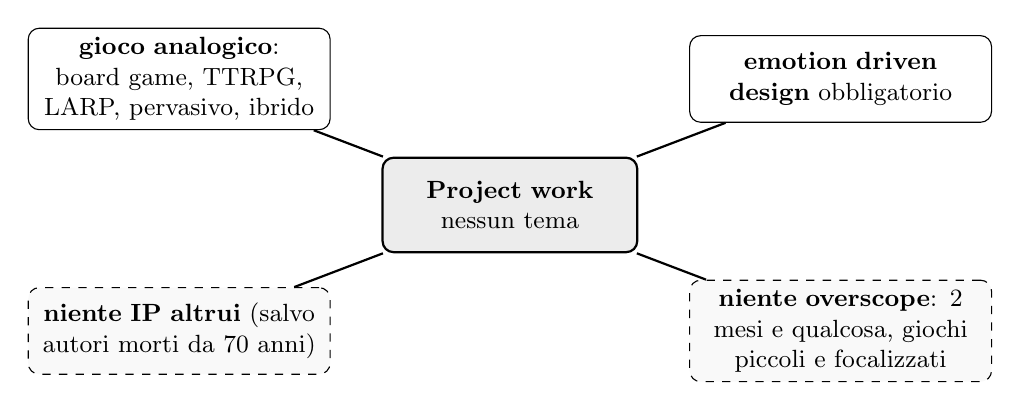
\begin{tikzpicture}[
    font=\small,
    centro/.style={draw, thick, rounded corners, fill=gray!15, text width=3.0cm,
      align=center, minimum height=1.2cm},
    vincolo/.style={draw, rounded corners, text width=3.6cm, align=center,
      minimum height=1.1cm, fill=white},
    no/.style={draw, dashed, rounded corners, text width=3.6cm, align=center,
      minimum height=1.1cm, fill=gray!5},
    linea/.style={thick}
  ]
  \node[centro] (c) at (0,0) {\textbf{Project work}\\ nessun tema};
  \node[vincolo] (a) at (-4.2,1.6) {\textbf{gioco analogico}: board game, TTRPG,
    LARP, pervasivo, ibrido};
  \node[vincolo] (b) at (4.2,1.6) {\textbf{emotion driven design}
    obbligatorio};
  \node[no] (d) at (-4.2,-1.6) {\textbf{niente IP altrui} (salvo autori morti da
    70 anni)};
  \node[no] (e) at (4.2,-1.6) {\textbf{niente overscope}: 2 mesi e qualcosa,
    giochi piccoli e focalizzati};
  \foreach \x in {a,b,d,e} { \draw[linea] (c) -- (\x); }
\end{tikzpicture}
\caption{Il \emph{mandate} del project work: due cose da fare (in alto) e due da
non fare (in basso, tratteggiate). Ricostruzione schematica della slide di
Daniele.}
\label{a7:fig:mandate}
\end{figure}

% ---------------------------------------------------------------------
\section{I gruppi}
\label{a7:sec:gruppi}

Poi i gruppi, tre gruppi da tre (tabella~\ref{a7:tab:gruppi}). La scelta è dei
docenti ed è ``insindacabile'', ma è basata sulle attività e sui task fatti
finora, ``sulla base di quello che vi abbiamo fatto fare negli ultimi giorni, come
lezioni, sulla vostra task e su quello che è stato un po' il nostro modo di
vedere''. Si è cercato di bilanciare anche gli \textbf{impegni di lavoro} di
ciascuno.

\begin{table}[htbp]
\centering
\begin{tabular}{@{}ll@{}}
\toprule
\textbf{Gruppo} & \textbf{Componenti} \\
\midrule
Gruppo 1 & Giordano, Nicola, Rita \\
Gruppo 2 & Gianmarco, Tancredi, Lorenzo Vergata \\
Gruppo 3 & Tiziana, Angelo, l'altro Lorenzo \\
\bottomrule
\end{tabular}
\caption{I gruppi del project work come li annuncia Daniele\protect\footnotemark.}
\label{a7:tab:gruppi}
\end{table}
\footnotetext{La trascrizione dice ``Giordano, Nicole, Rita, gruppo 2 Gianmarco,
Tancredi e Lorenzo V, gruppo 3 Tiziana, Angelo e Lorenzo''. ``Lorenzo V'' è Lorenzo
Vergata, come confermano poi i messaggi tra lui e Tancredi durante la pausa;
``Nicole'' è Nicola, a cui più tardi Beatrice dice che è nel gruppo ``con Giordano e
Rita''.}

Il progetto va sviluppato \textbf{durante il corso}: ``non vanno bene idee
pregresse, non portate nei vostri gruppi idee precedenti''. Le idee si sviluppano
insieme agli altri.

% ---------------------------------------------------------------------
\section{Le regole per lavorare in gruppo}
\label{a7:sec:regole}

Prima di lasciare la lezione a Beatrice, Daniele dà ``altri consigli per gli
acquisti''.

\paragraph{Rispettarsi.} ``La maggior parte del lavoro di un gruppo di sviluppo è di
\textbf{soft skill} più che di skill''. Bisogna capire come collaborare: se qualcuno
ha impegni di lavoro e fa fatica a garantire del tempo, ``partite da quello''. Non
si parte con ``un progetto grande come un castello disneyano'' per poi trovarsi
senza tempo; ci si dice invece ``io posso lavorare solo in questi momenti, lui o lei
solo in questi momenti'', e si cerca di fare ``qualcosa che abbia senso fare per il
tempo che abbiamo a disposizione''.

\paragraph{Taggare i docenti.} In caso di problemi si scrive ai docenti su
\textbf{Discord}, ma \textbf{taggandoli}: ``non lasciate messaggi senza taggarci,
se no li vedo una settimana dopo''. Oppure su \textbf{Telegram}.

\paragraph{Usare subito questi giorni.} Questi giorni vanno usati per il
\emph{brainstorming}: il tutoraggio con Ruggero è a breve (Daniele parla di ``48
ore'' per impostare il lavoro e capire che cosa fare).

\paragraph{Lavorare nel Drive.} Questa è una regola \textbf{obbligatoria}. Nel
Drive condiviso del corso ci sono le cartelle ``attività in classe'', ``dispense'',
``materiali didattici'' e ``project work''; dentro ``project work'' Daniele crea
tre cartelle, \textbf{gruppo 1}, \textbf{gruppo 2} e \textbf{gruppo 3}. Lavorare nel
Drive vuol dire evitare il più possibile di creare file fuori e caricarli dopo:
si aprono i Google Document lì e si lavora \textbf{in cloud}. Il motivo: se un
gruppo ha problemi e Daniele vuole aiutarlo, ha bisogno di vedere il
\textbf{processo mentale}, cioè che cosa è stato fatto nel documento, ``lo
\textbf{storico} del documento''. Un PDF o un \texttt{.docx} caricati così come
sono non hanno storico. Le cartelle vanno organizzate al meglio possibile; per
qualsiasi problema, ``basta chiedere''.

\paragraph{La dispensa sul brainstorming.} A seguito di questa lezione, ``tra stasera
e domani mattina'', Daniele registrerà una \textbf{dispensa}: il pezzo che venerdì
non c'è stato modo di fare, sul \emph{brainstorming} e sulla ricerca e sviluppo
``lato marketing'' e sugli strumenti di marketing nella ricerca e sviluppo. Metterà
a disposizione le slide e un video, con le slide del \textbf{brainstorming
strutturato}.

Nessuna domanda (``molti pollicioni, va bene''). Daniele ringrazia Bea ``per il
supporto e la condivisione'', saluta (``ci vediamo sicuramente il 12 di
ottobre'') e lascia la lezione.

% ---------------------------------------------------------------------
\section{Perché facciamo game design: due obiettivi}
\label{a7:sec:obiettivi}

``Ciao gruppo''. Beatrice comincia dando un po' di contesto: il corso è alla
\textbf{seconda edizione}, ci sono cambiamenti rispetto alla prima, e i docenti
stanno cercando di capire ``come rendervi il lavoro più agile e fattibile
possibile''. Nelle slide di oggi c'è molto, ``sarò onesta, credo troppo per la
lezione di oggi'', e quello che non si farà si riprenderà nella lezione successiva.
Il programma: ``mettere le mani in pasta'' per prepararsi ad affrontare un lavoro di
design; un po' di \emph{brainstorming} (da approfondire con i materiali di Daniele);
e una sorta di percorso di creazione di un gioco con un piccolo \textbf{esercizio di
design sprint}, a cui sarà dedicata la maggior parte della lezione. Alla fine del
corso i docenti chiederanno anche dei \textbf{feedback} su come è andato tutto.

Prima, però, un ``cappellino introduttivo'' sul \textbf{perché facciamo design}, già
anticipato nelle lezioni precedenti. Ci sono \textbf{due entità} che in questo
contesto si chiamano \textbf{obiettivi di design}:
\begin{enumerate}
  \item l'\textbf{obiettivo del gioco}, della produzione che si fa;
  \item l'\textbf{obiettivo personale} di chi progetta.
\end{enumerate}

\paragraph{L'obiettivo del gioco.} Un obiettivo di design del gioco, o del momento in
cui si sta facendo design, ha molte possibilità: raccontare un'esperienza di vita,
esplorare meccaniche o dinamiche, e così via; gli esempi della slide sono ``buttati
lì, sempre in brainstorming''. Si può decidere di fare un gioco per $N$ motivi, alcuni
personali e altri esterni al proprio bisogno personale.

Il punto è che \textbf{il motivo per cui affrontiamo la creazione di un gioco cambia
anche come progettiamo}. Beatrice vuole invitare la classe a ragionare su queste
cose, che spesso restano \textbf{ragionamenti interni} e invece è importante che
siano anche \textbf{condivisi}.

\paragraph{L'obiettivo personale.} L'obiettivo personale è semplice: rispondere alla
domanda \textbf{``perché sto facendo questo gioco?''}. Beatrice propone
\textbf{quattro categorie}, ``ma ce ne sono molte altre'', e probabilmente ne
emergeranno di nuove col crescere della disciplina; per la classe, i macro-obiettivi
saranno verosimilmente questi (figura~\ref{a7:fig:obiettivi}).
\begin{enumerate}
  \item \textbf{Voglio pubblicare un gioco.} Come gruppo di lavoro o come persona,
        voglio parlare a degli editori e pubblicare. Sotto questo cappello stanno sia
        la \textbf{pubblicazione con un editore} sia
        l'\textbf{auto\-pubblicazione}.
  \item \textbf{Voglio esprimere me stesso o me stessa.} È ``molto sottovalutato,
        troppo sottovalutato'': il gioco è uno strumento di espressione molto grande,
        che coinvolge anche altre persone. Magari non si vuole pubblicare né vendere,
        ma trasmettere davvero qualcosa che si è vissuto, qualcosa che si vuole
        raccontare; o si fa attivismo politico e si vuole un'attività che
        sensibilizzi sull'ecologia o su altri temi.
  \item \textbf{Voglio formare, informare o sensibilizzare.} Può sovrapporsi al
        punto precedente. Un gioco per insegnare meglio la matematica, per far
        conoscere un quartiere della propria città o un evento storico, per far
        crescere una competenza (aiutare le persone a parlare meglio in gruppo):
        ``$N$ situazioni di formazione''.
  \item \textbf{Voglio usare i giochi per il marketing e la comunicazione.} Portare
        l'attenzione su qualcosa: può essere un'espressione personale o una
        sensibilizzazione, ma anche un \textbf{prodotto} o un \textbf{servizio}. Lo si
        è visto con gli \emph{alternate reality game} del marketing, e in tante altre
        situazioni.
\end{enumerate}

\begin{figure}[htbp]
\centering
\begin{tikzpicture}[
    font=\small,
    domanda/.style={draw, thick, ellipse, fill=gray!15, text width=3.2cm,
      align=center, inner sep=2pt},
    ob/.style={draw, rounded corners, text width=3.3cm, align=center,
      minimum height=1.5cm, fill=white},
    freccia/.style={-{Stealth[length=2mm]}, thick}
  ]
  \node[domanda] (q) at (0,0) {\textbf{Perché sto facendo questo gioco?}};
  \node[ob] (p) at (-4.4,1.9) {\textbf{pubblicare}\\ con un editore o in
    autoproduzione};
  \node[ob] (e) at (4.4,1.9) {\textbf{esprimere me stesso/a}\\ raccontare,
    sperimentare, attivismo};
  \node[ob] (f) at (-4.4,-1.9) {\textbf{formare, informare, sensibilizzare}\\
    scuole, terzo settore, aziende};
  \node[ob] (m) at (4.4,-1.9) {\textbf{marketing e comunicazione}\\ prodotti,
    servizi, ARG};
  \foreach \x in {p,e,f,m} { \draw[freccia] (q) -- (\x); }
\end{tikzpicture}
\caption{Le quattro categorie di obiettivo personale proposte da Beatrice. ``Ce
ne sono molte altre''; esprimersi e sensibilizzare spesso si sovrappongono, e uno
stesso gioco può rispondere a più obiettivi.}
\label{a7:fig:obiettivi}
\end{figure}

% ---------------------------------------------------------------------
\section{Le competenze che ogni obiettivo richiede}
\label{a7:sec:competenze}

Ognuno di questi obiettivi personali richiede delle \textbf{competenze}, che ci si
fa ``in corso d'opera''. I docenti non si aspettano che gli studenti approfondiscano
ogni slide durante il corso, ma vogliono dire una cosa: se si crea un gioco, tutta
l'analisi di cui si è parlato (del mercato, delle persone, del target) va tenuta in
considerazione \textbf{in funzione dell'obiettivo}. Ogni obiettivo ha un modo
diverso di guardare il gioco e di produrlo. La slide mostra una ``carrellata'' di
competenze e conoscenze (tabella~\ref{a7:tab:competenze}).

\paragraph{Pubblicare con un editore.} Sono emerse domande anche dalla classe su come
capire che cosa sia meglio fare. Bisogna \textbf{conoscere il mondo della produzione}
di giochi da tavolo, di giochi di ruolo e di eventi ludici: chi esiste, che cosa fa,
a che prezzi mette fuori le cose, che tipo di prodotti vende già; se ci si riesce,
quante copie vengono vendute, quante persone comprano un biglietto. E
\textbf{conoscere le persone}: non solo ``c'è la casa editrice con il nome X'', ma
``all'interno ci lavorano X, Y, Z''. Partecipare agli eventi, mettersi in
connessione: sono tutte competenze, orientate a capire \textbf{come inserirsi} nelle
realtà che possono avere interesse a pubblicare.

\paragraph{Autoprodursi.} Le logiche sono diverse. Il mondo editoriale va conosciuto
comunque, perché in questo caso sono \textbf{competitor}; ma bisogna ragionare di più
verso il \textbf{pubblico}: capire come arrivare al momento in cui le persone
acquistano. Quindi parlare con gli utenti, affinare il marketing, analizzare i
competitor. E i competitor non sono solo quelli che fanno la stessa attività: per un
\textbf{evento dal vivo} un competitor può essere una fiera o un concerto, non per
forza un'attività di gioco; per un \textbf{gioco da tavolo formativo} un competitor
può essere un \textbf{corso}, non per forza un altro gioco. ``Immaginate i
competitor un po' più ad ampio spettro''. Infine, tutta una serie di informazioni
``non scontate'' e ``spesso prese sotto gamba'': \textbf{fiscalità e normative}.

\paragraph{Il GDPR: un'anticipazione.} Su questo, nella prossima lezione, Beatrice
farà ``un piccolo cappello'' sulle basi del \textbf{GDPR}, per poter raccogliere i
dati degli utenti e ricontattarli. È utile qualunque sia l'obiettivo: è sempre utile
avere, in una forma che permetta di risentirle, i dati delle persone con cui si è
venuti in contatto, che magari hanno testato il gioco, per tornare a scrivergli e
capire una serie di cose.

\paragraph{Esprimere se stessi.} Per sperimentare, per esplorare: qui ci sono
competenze ``spesso non raccontate, perché meno orientate al mercato'', che
riguardano \textbf{come trasmettiamo i contenuti} che vogliamo portare. È il lavoro
di \textbf{emotional design}, che ``sembra complicatissimo'', o comunque difficile da
definire; lo è, perché cambia per ogni gioco, ma col tempo si raffina sempre di più.
Chi vuole usare il gioco come sperimentazione personale, come linguaggio di dialogo
personale, deve capire bene quali sono i propri obiettivi: può essere ``voglio
comunicare la mia storia personale'', ma anche ``voglio trovare persone a me
affini'', o, ``banalmente'', ``voglio essere la persona che ha fatto il gioco più
conosciuto sulle \textbf{lumache da prato}''. Se è quello che si vuole raggiungere,
va bene: capito bene l'obiettivo, si capisce meglio tutto il resto, cioè
\textbf{che cosa voglio dire, a chi dirlo e perché} voglio dire determinate cose.

\paragraph{Formare, informare, sensibilizzare.} ``C'è un mondo'' su come si fa questo
design; qualcosa si vedrà nella prossima lezione, con le \textbf{escape room} e le
escape room formative. Per capire il mercato che può pagare queste attività, secondo
l'esperienza di Beatrice (``che non è onnisciente, ma è abbastanza puntuale al giorno
d'oggi''), le macro-voci in cui ci sono dei soldi, escludendo
l'\textbf{autofinanziamento} (che lei mette in una voce a sé), sono tre:
\begin{itemize}
  \item il \textbf{terzo settore} e i \textbf{bandi};
  \item il mondo delle \textbf{scuole} e della \textbf{formazione};
  \item la \textbf{formazione aziendale}: \emph{learning and development}, risorse
        umane e simili.
\end{itemize}
Sono tre mondi con logiche ``completamente diverse'' da quelle viste prima, e
Beatrice non ci si sofferma, perché non è il fulcro del corso. Ma già queste voci
bastano per sapere dove approfondire, se si vuole fare un gioco formativo: che cos'è
il terzo settore e che cosa significa proporgli dei giochi; che cosa sono i bandi
pubblici e quali enti li finanziano; e lo stesso per le scuole e per le aziende. E
poi c'è ``il magico mondo della \textbf{formazione finanziata}'', che sta sempre
sotto il cappello delle risorse umane: già googlando queste due parole si trovano
molte situazioni in cui si inserisce la proposta di giochi.

\paragraph{Il marketing.} Qui la parte principale da sapere è quella già vista
sull'\textbf{analisi del target} e sull'individuazione delle persone da coinvolgere.
Beatrice non si sofferma, perché secondo lei il marketing ``arriva dopo'': quando si
è progettato un po' di più (vale anche per la formazione) e si è sperimentato quello
che si è in grado di fare, allora si possono immaginare giochi per il marketing, che
sono giochi che portano l'utente a fare determinate cose. Per chi vuole approfondire,
la cosa principale è questa: si parla con delle \textbf{aziende}, e le aziende,
``anche le più virtuose'', hanno l'obiettivo di ``fare dei soldini''. Bisogna saper
rispondere alla domanda \textbf{``come aiuta l'azienda a fare più soldi?''}. I casi
sono due: \textbf{aumenta le vendite}, oppure fa aumentare \textbf{quanto l'azienda è
conosciuta}, o, se è conosciuta male, ne modifica in positivo la
\textbf{reputazione}. ``Non è un mondo bellissimo, ma è un mondo che esiste'': giochi
di questo tipo esistono tantissimo, e spesso non sono neanche raccontati come tali.
Beatrice lo dice perché magari si ha ``il gioco migliore del mondo'' e non si sa come
pagarsene lo sviluppo: questo può essere un modo.

\begin{table}[htbp]
\centering
\begin{tabular}{@{}p{3.0cm}p{9.6cm}@{}}
\toprule
\textbf{Obiettivo} & \textbf{Che cosa bisogna conoscere} \\
\midrule
Pubblicare con un editore & il mondo della produzione (chi c'è, che cosa fa, a che
prezzi, quanto vende); le persone dentro le case editrici; eventi e contatti \\
Autoprodursi & il mondo editoriale come competitor; il pubblico; marketing;
competitor ``ad ampio spettro'' (una fiera, un concerto, un corso); fiscalità e
normative; GDPR \\
Esprimere se stessi & come trasmettere i contenuti; \emph{emotional design}; che
cosa voglio dire, a chi e perché \\
Formare e sensibilizzare & terzo settore e bandi; scuole e formazione; formazione
aziendale (\emph{learning and development}, risorse umane); formazione finanziata \\
Marketing & analisi del target; ``come aiuta l'azienda a fare più soldi?'':
vendite, notorietà, reputazione \\
\bottomrule
\end{tabular}
\caption{Le competenze per obiettivo personale, ricostruite dalla carrellata di
Beatrice.}
\label{a7:tab:competenze}
\end{table}

\paragraph{Lo stesso gioco, più obiettivi.} Uno stesso gioco può rispondere a più
obiettivi. Si fa un gioco formativo, o un gioco per esprimersi, e si scopre che
potrebbe essere venduto a un'azienda, rispondere a un bando, entrare
perfettamente nel catalogo di un editore estero ``che non conoscevate fino a ieri'',
o di un editore italiano conosciuto in fiera. Quello che interessa a Beatrice è che
gli studenti abbiano chiari \textbf{gli interessi del mondo a cui parlano}, quando
hanno un gioco in progettazione o già fatto. Se si è consapevoli degli interessi
degli altri e del proprio obiettivo personale, ``diventa molto più facile il
dialogo''. Riuscire poi a vendere e ``imbroccare le cose giuste'' è un altro tema;
ma questi due elementi vanno avuti \textbf{prima}.

\paragraph{Approfondimento: il perché del designer.} Il tema dell'obiettivo personale
ha un parallelo in \emph{The Art of Game Design} di Jesse Schell, che apre il libro
non dal gioco ma dal designer stesso (``in the beginning, there is the designer''),
e più avanti dedica capitoli interi al rapporto con il \emph{cliente} e al
\emph{pitch}, cioè proprio al ``dialogo'' con gli interessi altrui di cui parla
Beatrice. Nella lezione, però, la distinzione tra
\emph{obiettivo del gioco} e \emph{obiettivo personale} ha soprattutto una funzione
pratica: è il primo argomento della chiacchierata iniziale del design sprint.

% ---------------------------------------------------------------------
\section{Il design sprint}
\label{a7:sec:sprint}

``Ora sono andata un po' veloce, e sono comunque lenta rispetto agli orari'':
Beatrice passa all'esercizio. Condivide un altro file (``che voi vedete bruttarello
qui e che poi vi caricherò''); chi non lo legge può mandarle ``un'emoji triste o
buffa''. Ha preparato \textbf{due moduli}; quello di adesso è su \textbf{come fare una
sessione di design sprint}.

\paragraph{Che cos'è.} Il design sprint si può usare per $N$ cose: ``dal decidere
come arredare casa a come risolvere il problema di non avere abbastanza soldi per
fare la spesa'', per qualunque problema. \textbf{Non è uno strumento nato per il game
design}: è nato per ragionare su problemi di progettazione e cercare soluzioni di
design. Beatrice lo ha \textbf{adattato all'uso sui giochi}, e lo ha diviso in
\textbf{fasi}, perché sono le fasi che invita i gruppi a provare a seguire. Il file
verrà caricato nella cartella condivisa degli strumenti. Oggi racconterà la prima
fase, ma la salterà, e si partirà dalla seconda.

\paragraph{Un invito, non un obbligo.} È ``uno strumento in più che vi dà una
direzione in caso la direzione non riusciate a trovarla in breve tempo''. Beatrice lo
dice apertamente: l'anno scorso alcuni gruppi hanno investito molto tempo in alcune
fasi della progettazione e non sono riusciti a concludere il gioco. Quest'anno si
vuole evitarlo, e per questo ci sono \textbf{due strumenti}: questo, e quello che si
vedrà alla fine di questa lezione e all'inizio della prossima, cioè tutte le voci che
compongono la progettazione di un gioco, per avere una \textbf{visione d'insieme} e
poter dire: ``abbiamo queste settimane prima del pitch e questi mesi prima della
consegna''. Ognuno ha un lavoro, una famiglia, dorme, mangia, fa cose che occupano
tempo: bisogna farsi ``dei conti pratici'', un tot di ore per una parte e un tot per
un'altra.

\paragraph{Il project management che non c'è.} Tutto questo fa parte del
\textbf{project management} di un progetto, e Beatrice avverte che nel mondo del
lavoro, ``nel gaming perlomeno'', \textbf{non esiste}: nella slide in cui sono state
presentate tutte le professioni non c'è un \emph{project manager} dei giochi, perché
le aziende sono ``ancora un po' in costruzione'' su questo lato; quelle italiane
almeno, mentre all'estero ci sono casi molto diversi, e nel videogioco funziona in un
altro modo. Questi strumenti vanno conosciuti per essere più consapevoli di
\textbf{come si funziona come persone}, preparandosi al fatto che il mondo esterno
non sempre segue logiche di organizzazione e ``più spesso bisogna un po' navigare le
onde''. Per il corso, però, sono molto utili: quando il gruppo ``per un attimo si
perde'', si può tornare a fare il punto con questi strumenti.

\subsection{Le fasi del file}
\label{a7:sec:fasi-file}

Beatrice scorre i ``titoloni'' del documento (figura~\ref{a7:fig:sprint}).
\begin{enumerate}
  \item \textbf{La chiacchierata iniziale}, che oggi si salta (si veda sotto).
  \item \textbf{Definire l'obiettivo di gruppo} del gioco: proposte e votazioni.
  \item Una piccola sessione di \textbf{ricerca e sviluppo} basata sull'obiettivo.
  \item Una prima sessione di \textbf{brainstorming} su quello che emerge, per
        rispondere all'obiettivo.
  \item La \textbf{valutazione} di tutto il brainstorming: che cosa si tiene e che
        cosa si butta, di tutte le idee uscite.
  \item Da lì in poi, l'\textbf{assegnazione dei ruoli}: chi fa cosa, con che tempi.
\end{enumerate}
Oggi si faranno le fasi dalla seconda in poi, fingendo che la classe sia un unico
grande gruppo di \textbf{nove persone} che inventa un gioco: ``faremo tutto quello
che serve per fare un brainstorming per avere il pitch del gioco''. Sarà un gioco
``del gruppo tutto'', quindi non lo si potrà portare a conclusione nel corso: serve
ad allenarsi con lo strumento.

\begin{figure}[htbp]
\centering
\begin{tikzpicture}[
    font=\small,
    fase/.style={draw, thick, rounded corners, text width=2.5cm, align=center,
      minimum height=1.3cm, fill=white},
    oggi/.style={fase, fill=gray!15},
    saltata/.style={fase, dashed, fill=gray!4},
    freccia/.style={-{Stealth[length=2mm]}, thick},
    nota/.style={font=\scriptsize\itshape, text width=2.5cm, align=center}
  ]
  \node[saltata] (f0) at (0,0) {chiacchierata iniziale (30 min)};
  \node[oggi, right=0.5cm of f0] (f1) {obiettivo del gioco: post-it e voto};
  \node[oggi, right=0.5cm of f1] (f2) {ricerca e sviluppo};
  \node[oggi, right=0.5cm of f2] (f3) {brainstorming su meccaniche, tipo,
    narrazione, setting};
  \node[oggi, below=1.1cm of f3] (f4) {voto, poi mappa impatto-sforzo};
  \node[oggi, left=0.5cm of f4] (f5) {percorso dell'utente};
  \node[fase, left=0.5cm of f5] (f6) {chi fa cosa, con che tempi};
  \node[fase, left=0.5cm of f6] (f7) {progettazione e sviluppo};
  \draw[freccia] (f0) -- (f1);
  \draw[freccia] (f1) -- (f2);
  \draw[freccia] (f2) -- (f3);
  \draw[freccia] (f3) -- (f4);
  \draw[freccia] (f4) -- (f5);
  \draw[freccia] (f5) -- (f6);
  \draw[freccia] (f6) -- (f7);
  \draw[freccia, dashed] (f7.north) -- node[midway, right=2pt,
    font=\scriptsize, align=left] {quando ci si perde:\\ di nuovo al voto}
    (f1.south west);
  \node[nota, above=0.1cm of f0] {saltata a lezione};
\end{tikzpicture}
\caption{Le fasi del design sprint adattato da Beatrice per il corso. In grigio le
fasi toccate a lezione (alcune solo raccontate per mancanza di tempo); la
chiacchierata iniziale è saltata. La freccia tratteggiata riassume il consiglio
``quando vi perdete, andate a votazione''. Ricostruzione schematica del file.}
\label{a7:fig:sprint}
\end{figure}

\paragraph{Una scaletta per il corso, non il design sprint.} Beatrice lo ripeterà più
avanti, a Nicola: la scaletta \textbf{non è una fase standard}, ``non voglio che vi
portiate a casa che il design sprint è tutto così, sempre, a queste fasi''. Prende
delle metodologie e le porta in una scaletta pensata per il corso.

\subsection{La chiacchierata iniziale}
\label{a7:sec:chiacchierata}

La prima fase è un \textbf{allineamento di gruppo}, e oggi si salta. Le domande:
\begin{itemize}
  \item quali sono i nostri \textbf{obiettivi personali} (quelli visti prima)?
        ``Magari il mio obiettivo in questo corso è provare a sperimentare. Oppure
        Lorenzo vuole fare un gioco per provare a venderlo da qualche parte, oppure
        io voglio fare un gioco per raccontare la storia della mia famiglia''.
        Allinearsi non vuol dire che sarà quello che si porterà a casa, ma che si
        conoscono i desiderata degli altri e c'è uno spazio per raccontare i propri;
  \item \textbf{che competenze ho}? A quali progetti ho già lavorato, e che cosa
        facevo in quei progetti?
  \item la ``domandona'': in questo corso voglio lavorare sulle \textbf{stesse
        competenze} su cui ho lavorato in passato, o ci sono attività che non ho
        ancora esplorato, che non ho mai fatto e vorrei esplorare qui? ``Non ho mai
        scritto testi, ma qua mi andrebbe di provare'', ``non ho mai fatto
        illustrazioni e qua mi andrebbe di vedere'': qui si può fare, e conviene
        capire in che ruolo mettere le proprie competenze. (Beatrice corregge anche
        un refuso nel file, in diretta.)
\end{itemize}
Per gruppi di tre persone, \textbf{30 minuti} bastano e avanzano: uno scambio in cui
``ognuno sa la situazione delle altre persone''. Beatrice invita a farla quando
inizierà il lavoro di gruppo.

\paragraph{Approfondimento: lo Sprint di Google Ventures.} Il \emph{design sprint}
nella forma più nota è quello descritto da Jake Knapp, con John Zeratsky e Braden
Kowitz, nel libro \emph{Sprint} (2016), nato a Google Ventures: cinque giorni per
passare da un problema a un prototipo testato con utenti reali, con passaggi molto
simili a quelli della lezione (mappare il problema, raccogliere ispirazioni,
proporre soluzioni individualmente e in silenzio, votare con adesivi a pallino,
decidere). L'adattamento di Beatrice ne conserva il cuore (lavoro individuale
silenzioso, presentazione, voto a pallini, tempi rigidi) ma lo piega ai tempi e agli
scopi di un corso: niente giornate intere, e la prima fase dedicata alle persone del
gruppo, non al problema.

% ---------------------------------------------------------------------
\section{La lavagna di Canva}
\label{a7:sec:canva}

``Ora vi condivido questa fantastica lavagna''. Per il \emph{brainstorming} ci sono
``tantissimi'' strumenti e modalità; oggi si usa il design sprint come modalità e una
\textbf{lavagna di Canva} come strumento.

\paragraph{Entrare.} Il link nella chat non è cliccabile, né si riesce a copiarlo
(``nemmeno copia e incolla''). Qualcuno lo copia a mano nella barra del browser e
riesce a entrare; un altro lo mette su Discord, dove ``funziona'', anche se a qualcuno
risulta che dal link di Discord non ha l'autorizzazione (``essendo che il link l'ho
copiato io, magari non ci sono i permessi''). Alla fine Beatrice crea un link
accorciato, ``più dettabile'' (\texttt{urli.it/31GRXQ}, secondo la trascrizione).

\paragraph{Gli strumenti in generale.} Canva è uno strumento per sessioni di
\emph{brainstorming} simile a molti altri; un altro è \textbf{Miro}, ``ma ce ne sono
davvero tanti''. Beatrice usa Canva perché è il più comodo per lei. L'impostazione
della lavagna \textbf{simula un incontro dal vivo}: le attività di oggi si possono
fare in digitale, a distanza, con uno strumento di questo tipo, oppure dal vivo con
\textbf{carta e penna}, un tavolo dove appoggiare i bigliettini, un muro dove
attaccare i post-it. ``Ve lo dico perché può essere utile anche per il futuro''.

\paragraph{Come si usa.} Beatrice ha ``loccato'' (bloccato) gli elementi della
lavagna, così che nessuno sposti per errore le cornici; si può selezionare e
zoomare liberamente (avvicinandosi le lavagne ``diventano più grandi''), ma bisogna
stare attenti a non cancellare il lavoro degli altri. Per cancellare: si seleziona
l'elemento e si preme il tasto di cancellazione, oppure il piccolo cestino nel menu
dell'elemento. Gli strumenti utili sono nel \textbf{menu a sinistra} di Canva, che ha
sette voci (Canva AI, Modelli, Elementi, Testo, Brand, Caricamenti,
\textbf{Strumenti}); sotto \textbf{Strumenti} (l'icona con una ``pennina'') ci sono,
tra gli altri, il \textbf{testo} e i \textbf{foglietti adesivi}: ``veri e propri
post-it, come quelli che usereste dal vivo''. Si sceglie un colore, il post-it compare,
lo si ingrandisce o rimpicciolisce e ci si scrive sopra.

\paragraph{Le prove.} La prova serve anche ad allinearsi sullo strumento, ed è
movimentata. I post-it compaiono uno dopo l'altro (``Giordano, anche Lorenzo'',
``vedo una C'', ``Rita sta scrivendo''); Gianmarco entra senza il suo account e
compare come ``Leone Marino'', uno dei nomi di animale che lo strumento assegna
agli utenti anonimi\footnote{La trascrizione dice ``è come l'anonimo di Giuseppe'':
con ogni probabilità il riferimento è agli ``animali anonimi'' con cui Google e
altri servizi mostrano chi partecipa senza account.}. Si scopre che se la
lavagna di base è bloccata non si riesce a scrivere nei post-it (``io l'ho imparato
adesso, perché credevo non funzionasse così''), e Beatrice sblocca. Qualcuno sposta
per sbaglio l'intera cornice (``oh mio Dio, sono uscito, e qualcuno ha spostato tutta
la lavagna''), qualcuno ha post-it finiti fuori dalla lavagna o giganteschi, una
studentessa (``una grafica fissata con l'impaginazione'') prova a riallineare
tutto. Angelo, che è collegato \textbf{dal cellulare}, non riesce a trascinare il
post-it (``non me lo fa trascinare''); Beatrice lo guida passo per passo e alla fine
decide di creargli lei dei post-it con il proprio nome sopra, che Angelo userà
(``ci ricorderemo che i tuoi post-it sono quelli con il nome di Beatrice''), anche
se poco dopo Angelo riesce a crearne uno da solo (``ce l'ho fatta'').
``Dal telefono è anche più complicato, è normalissimo''. Beatrice avverte che
\textbf{Miro è un po' più intuitivo} di Canva, e che servirà molto spazio: il gioco di
fare le cose piccole e zoomare sarà utile soprattutto nella ricerca e sviluppo.

\paragraph{Lo strumento conta il giusto.} ``Di tutto questo, lo strumento ci interessa
il giusto'': si può usare Miro, si possono scrivere le cose a mano. \textbf{Ci
interessa il procedimento}.

% ---------------------------------------------------------------------
\section{Prima fase: che obiettivo vorrei dare a questo gioco?}
\label{a7:sec:fase1}

La domanda della prima fase è \textbf{``che obiettivo vorrei dare a questo
gioco?''}. Le regole:
\begin{itemize}
  \item ognuno scrive \textbf{al massimo tre risposte}, e almeno una;
  \item \textbf{una risposta per post-it};
  \item non è il genere del gioco e non sono le meccaniche: è ``più a volo
        d'aquila'', quello che si vorrebbe che il gioco ottenesse; può riguardare
        anche le \textbf{emozioni}, cioè che cosa far provare alla persona che gioca.
\end{itemize}
Gli esempi del file mescolano apposta livelli diversi: ``un gioco formativo per
insegnare l'inglese'', ``un gioco con dei pinguini blu'', ``un GDR per sensibilizzare
sulla lotta di classe'', ``un gioco fantasy sulla vendetta'', ``un gioco con delle
pedine gigantesche'', ``un gioco che faccia esplorare un quartiere''.

\paragraph{I timer.} E qui la cosa da ricordare di tutto il procedimento:
\textbf{mettere i timer}. Nei processi creativi di gruppo, e probabilmente lo si è già
visto succedere, ci si fa prendere da quello che sta avvenendo, dai dialoghi, dalle
idee che emergono. Beatrice richiama la lezione precedente su \textbf{divergenza e
convergenza}: c'è un momento in cui si apre, si esplora, si buttano idee; ma ``a un
certo punto bisogna \textbf{quagliare}''. Darsi un tempo di orologio dice fino a
quando si esplora; quando suona il timer, bisogna riportare in ordine la situazione.
``È la cosa importante di tutto il processo: dare dei tempi e provare a
rispettarli''. Il primo timer è di \textbf{5 minuti} (``dai 5 ai 10'').

\paragraph{Gianmarco arriva.} Gianmarco, ``arrivato un po' in corsa'', chiede il
contesto: si può buttare qualsiasi idea? È un esercizio, risponde Beatrice, per
imparare a fare \emph{brainstorming} e poi mettere in ordine le idee: ``vai pure
libero''.

\paragraph{La parola proibita.} Mentre scrivono, Rita avverte i compagni: qualcuno
ha scritto \emph{divertire} su un post-it, e ``dovremmo evitare di usare questo
verbo''\footnote{Il riferimento è alla regola, ricorrente nel corso, per cui ``far
divertire'' non è un obiettivo di design: è troppo generico per orientare le
scelte.}, ``conviene modificarlo prima che lo veda qualcuno'' (Ruggero, si
capisce). Beatrice: ``Io non dirò niente, però è un ottimo consiglio''. Del resto,
aggiunge, sono idee che non verranno condivise con gli altri docenti: è un esercizio
per imparare la procedura, che non è neanche detto si userà esattamente così. Le idee
di oggi possono avere vita propria e crescere, ``ma non in questo corso'': i gruppi
del progetto partiranno da zero.

% ---------------------------------------------------------------------
\section{Il racconto delle idee}
\label{a7:sec:racconto}

Prima della votazione, che Beatrice anticipa (si veda la
sezione~\ref{a7:sec:votazione}), \textbf{ognuno racconta che cosa ha scritto} e dice
\textbf{dove sono} i suoi post-it, così che tutti possano trovarli sulla lavagna. In
questa fase valgono due regole:
\begin{itemize}
  \item le altre persone possono fare \textbf{solo domande}: chiarimenti su che cosa
        si intende, su perché è emersa un'idea; ``tutte le domande che vi vengono in
        mente vanno benissimo'', anzi Beatrice invita a farle, perché ``c'è ancora
        tanto che può uscire'';
  \item \textbf{niente commenti}, ``né nient'altro''. Se non si hanno domande, non si
        dice nulla.
\end{itemize}
E Beatrice si fa da parte: ``fate finta che io non esista''. Ricorderà solo di dire
dove sono i post-it; il gruppo deve autogestirsi, come in un vero lavoro di gruppo
in cui nessuno dà la direzione. Poi si accorge di aver dimenticato il timer anche
qui: tutte le idee vanno raccontate in circa \textbf{15 minuti}, ``tenetene conto
quando fate le domande, quando rispondete, quando raccontate''.

\subsection{Rita}
\label{a7:sec:idee-rita}

Rita (post-it arancione, rosso e giallo, sovrapposti nell'angolo in alto a sinistra)
ha scritto tre idee.
\begin{description}
  \item[Un gioco educativo.] Si è avvicinata a questo mondo con l'idea di dare
        qualcosa in più alle nuove generazioni: è quello che l'ha spinta a diventare
        game designer.
  \item[Un gioco che costringe le persone a collaborare.] Quando la collaborazione è
        necessaria per raggiungere un obiettivo, bisogna affrontare problemi con se
        stessi e con gli altri, e questo è costruttivo e stimolante per tutti. È anche
        il suo approccio alla vita: ``condividere, collaborare per imparare''.
  \item[Un gioco sull'arte.] È la sua più grande passione: avvicinare le persone a
        un'arte ``non proiettata verso l'IA''.
\end{description}
Le domande. Il gioco sull'arte è sulla storia dell'arte, i grandi pittori, o un gioco
in cui \textbf{le persone fanno gli artisti}? La seconda: avvicinarle alla disciplina
in maniera attiva; e in effetti, osserva Rita, potrebbe rientrare nel gioco educativo,
con le scuole. Il gioco educativo, per che età e in che contesto? Non ci ha ancora
pensato nello specifico, ma pensava a bambini che stanno crescendo, elementari e
medie: per gli adolescenti ci vuole qualcosa di più attivo e stimolante a livello
emotivo, forse un LARP. Poi chiede lei un parere a una compagna con esperienza di
questi giochi: ci sono fasce d'età più interessate a certi tipi di gioco?
``Dipende'', risponde la compagna: si sente il gruppo, e se il gioco è educativo lo
si orienta anche, per esempio decidendo se farlo competitivo o no. A lei è sempre
piaciuto \textbf{mescolare competizione e collaborazione}: le \textbf{cacce al
tesoro} sono notoriamente competitive, ma le sue richiedevano sempre una
collaborazione tra i gruppi, e alla fine \textbf{il tesoro era per tutti}: c'era la
soddisfazione di chi era arrivato primo, ma il premio era di tutti. ``Bello, e
stimolante, perché si deve collaborare per raggiungere un obiettivo''.

\subsection{Nicola arriva}
\label{a7:sec:nicola}

A questo punto entra Nicola. Beatrice gli spiega in breve che cosa sta succedendo:
un esercizio di design sprint, ``una metodologia, anzi varie metodologie che
riguardano tante forme di design, non solo quello dei giochi'', per avere una
direzione quando un gruppo si perde o non sa come allinearsi; la prima fase è
rispondere a ``che obiettivo vogliamo dare al gioco''; i compagni hanno dato tre
idee ciascuno, che ora si leggono e poi si votano. E gli dice il suo gruppo: ``sei nel
gruppo 1, con Giordano e Rita'', ``non per motivi'', lo rivedrà nelle slide che
Daniele caricherà. Nicola entra nella lavagna come ``Nick''.

Poco dopo, Nicola chiede ``un quick check-up'': si sente ``in alto mare'', ``una
zavorra''. I post-it sono già divisi in gruppi? Sono concept di personaggio o di
gioco, di ogni singola persona? Si stanno comparando? Beatrice riconosce di non
essersi spiegata abbastanza e rispiega: si sta \textbf{testando la metodologia},
fingendo di essere un unico gruppo di nove da cui deve uscire ``una bozza di gioco'';
la scaletta non è standard ma costruita per il corso; per decidere l'obiettivo del
gioco ognuno butta giù idee in silenzio sui post-it, poi le si leggono (``una fase di
brainstorming aperto'') e infine le si vota.

Nicola chiede com'è il voto: qualitativo o quantitativo? Si vota sulla quantità di
contenuto, sulla tipologia, ``un voto vale più di un altro''? Nessun voto vale più di
un altro, risponde Beatrice: ognuno avrà \textbf{sei voti}, ``immagina di avere sei
pallini adesivi'', e può metterli anche tutti sulla stessa idea. A Nicola lo schema
ricorda quello studiato in \textbf{organizzazione aziendale}, quando si avvia un
progetto; Beatrice conferma che il design sprint si usa in moltissimi contesti, ``molto
sulle soluzioni da proporre'', anche in sociologia. Nicola chiede ancora se c'è stata
una spiegazione prima del lavoro: c'è stata una piccola introduzione sui motivi per cui
si fa design (recuperabile dalle slide o dalla registrazione), e poi ci si è buttati
sulla domanda. Infine: ci sono linee guida, ``o siamo randomici''? ``Per ora è tutto
libero, rimaniamo leggerissimi''. Nicola si scusa con la classe per il tempo rubato.

\subsection{Lorenzo Vergata}
\label{a7:sec:idee-vergata}

Lorenzo Vergata (post-it sopra quelli di Rita) presenta tre idee, mentre ``qualcuno
ha mosso la lavagna'' e per un momento ``è scomparso tutto''.
\begin{description}
  \item[I funghi.] \textbf{Esplorazione del bosco per sensibilizzare sulle specie
        fungine e sul rispetto della natura}, ``semplicemente perché siamo in periodo
        di funghi'': la prima cosa che gli è venuta in mente.
  \item[Frenetismo.] Partite rapide, ``quasi caotiche dall'esterno, ma
        pseudo-organizzate dall'interno fra i giocatori''. Si è chiesto che cosa cerca,
        a 26 anni, in un gioco: non partite lunghe, ma frenesia. Frenesia, quindi,
        ``per gente neolaureata e simile''.
  \item[Paura.] Nascondino; fuggire da qualcuno all'aperto, senza luci; o in casa,
        staccando la corrente all'inizio del gioco. ``Il gioco deve far paura'':
        senza aver fatto ricerca, pensa che non ci siano molti giochi che sfruttano la
        paura dei giocatori come dinamica.
\end{description}
Le domande, e qualche commento che sfugge alla regola. L'idea della paura è pensata
come un \textbf{LARP}, all'esterno, o come un gioco da tavolo? Lorenzo pensa che il
modo più semplice di creare paura sia un LARP, ma ``nulla toglie'' di farlo da tavolo,
studiando come un gioco da tavolo possa incutere timore. Una compagna osserva che la
paura si definisce in tanti modi: \textbf{pressione}, \textbf{ansia} (più facili da
tavolo) e \textbf{jumpscare} (più da LARP); bisognerebbe dare una dimensione al
concetto, ma è ``una bella sfida''. Le ricorda quando da ragazzina giocava a
\textbf{guardie e ladri} al mare, di notte, nelle case degli amici: si creava un
clima di paura e tensione, anche perché ci si facevano gli scherzi.

Un altro studente, che gioca ``per la maggior parte del tempo'' a giochi di ruolo da
tavolo\footnote{Dal contesto, con ogni probabilità Nicola, che poco dopo si presenta
come ``un grande giocatore di TTRPG''.}, conferma che la paura è ``un fantastico
strumento'', ma pone un problema: se diventa un \textbf{gioco pervasivo}, c'è un
\textbf{danno collaterale}, cioè \textbf{spaventare chi non gioca}. ``Immagino una
persona che corre a mezzanotte in giro per Roma urlando di paura'': terrificante per
chi la vede, e si coinvolgono persone che non vorrebbero provare quella paura.
Lorenzo concorda: bisognerebbe tarare, andando più verso quello che diceva la
compagna, cioè il momento in cui sei nascosto e senti che chi ti cerca è ``letteralmente
a fianco a te'', e ti pervadono paura e ansia. Ma ``basta poco'' per tirare in mezzo
estranei: chi vede una persona che ne insegue un'altra che cerca di nascondersi
``chiama la polizia al minuto zero''. Se sono bambini di sei anni, ``stanno
giocando''; se vedi un ventenne, ``che cosa sta accadendo?''.

Infine l'esplorazione del bosco: come sarebbe, come gioco? Una guida che ti porta nel
bosco? ``Fatta sul posto è tosta'': sarebbe semplicemente una gita con un
\textbf{micologo}. Ma \textbf{da tavolo} si potrebbe fare. Sul fronte della natura si
possono inserire meccaniche che \textbf{simulano il comportamento dei funghi}: sotto
di loro c'è il \textbf{micelio}, che fa da rete di comunicazione tra le piante, e ne
potrebbe uscire un gioco ``pseudostrategico''. Sulla \textbf{commestibilità} si può
immaginare uno scontro carta contro carta, una specie di sasso-carta-forbice: ``il
fungo buono te lo annullo con questo cattivo'', mentre certi funghi che ``sembrano
buoni'' rovinano tutto il raccolto, cioè una sola carta può rovinare molte carte di
funghi buoni. ``Potrebbe anche essere frenetico, chissà''.

\subsection{Tancredi}
\label{a7:sec:idee-tancredi}

Tancredi ha scritto in modo ``molto più riassunto''.
\begin{description}
  \item[Un gioco cooperativo.] È ``un grande fan dei cooperativi'', anche piccoli,
        come \emph{Hanabi}\footnote{La trascrizione dice ``Anabis''.}, \emph{Sky Team},
        \emph{Quicksand}: gli piace molto la meccanica della cooperazione.
  \item[Un gioco per il terzo settore.] Riprende la categoria vista prima, ma senza
        grandi idee: per questo tipo di gioco sarebbe importante capire \textbf{per chi}
        lo si fa, e non sa quanto sia realizzabile nel loro caso.
  \item[Un GDR.] Non conosce praticamente per niente i giochi di ruolo, li ha
        scoperti in queste lezioni: ``perché no?'', provare a sperimentare quel
        settore.
\end{description}
Che cosa aveva immaginato per il terzo settore? Secondo Tancredi un modo sarebbe
cercare delle realtà, anche solo su internet, sui loro siti, e capire che cosa
potrebbe essere interessante per loro, ``anche se poi non glielo si propone
veramente, perché questa è un'esercitazione''; con l'obiettivo di dare una mano,
diffondere quello che fanno. Un compagno racconta (più un commento che una domanda)
di aver giocato \emph{Nemesis: Retaliation} dal vivo nella modalità semicooperativa,
con i traditori, e ora online su \textbf{Board Game Arena}\footnote{La trascrizione
scrive ``BGA'', la sigla abituale del sito.} con più o meno gli stessi amici, in
modalità cooperativa, usando la chat: ``stratosferico, così mi diverto''. Se invece
``a un certo punto uno ti dà una ginocchiata sui denti''\ldots{} Tancredi: in
associazione ``quasi mai nessuno vuole fare cooperativi'', e lui è sempre lì; gli
piacciono anche i competitivi, ma certi giochi ``vale la pena giocarli così''.

\subsection{Tiziana}
\label{a7:sec:idee-tiziana}

Tiziana (post-it sotto quelli di Tancredi) ha scritto tre idee.
\begin{description}
  \item[Un board game, di costruzione, gestionale ambientato.] Le piacerebbe fare
        esperienza di costruzione di un gioco da tavolo e non saprebbe da che parte
        cominciare (come Tancredi con i giochi di ruolo: ``non ho idea, quindi mi
        piacerebbe provare''). Un \textbf{gestionale} perché le piace l'aspetto
        gestionale, ma \textbf{ambientato}, ``non so se è una chimera''.
  \item[Un'escape room per far divertire.] ``Lo so che non devo usare divertire, ma
        non sono riuscita a trovare nessun'altra cosa'', e soprattutto far divertire
        lei mentre la costruisce. E far nascere la \textbf{collaborazione}. Dal vivo o
        da tavolo, entrambi vanno bene; il tema non lo sa. Le piacciono gli
        \textbf{indovinelli}, trovare soluzioni; ma vorrebbe enigmi \textbf{misti}, non
        tutti dello stesso tipo, perché quando sono tutti uguali diventano ``o troppo
        cervellotici o ripetitivi''.
  \item[Un gioco interattivo per far conoscere la città.] Una parte di essa, perché
        Roma ``è abbastanza gigantesca''; l'aveva immaginato coinvolgendo perfino i
        \textbf{passanti}, ``ma non so se sia fattibile''.
\end{description}
Tancredi chiede: quando parli di gestionale, hai un riferimento? Un gioco economico,
con competizione e interazione molto alte, o qualcosa di meno interattivo,
``più German''? Tiziana non lo sa: da giocatrice è più ``mi coltivo il mio orticello''
(gli economici interattivi ``non sono i miei preferiti''), ma potrebbe essere anche
interattivo: intendeva la \textbf{gestione delle risorse} in generale. La cosa
fondamentale è che sia ambientato, ``che senti di essere in quel posto''. Un
compagno le suggerisce \emph{Akropolis}, per l'ambientazione e per l'idea di
costruire la propria città con tessere di tre esagoni sovrapposte, in cui i colori che
restano in cima diventano i quartieri: un approccio per non renderlo ``troppo
gestionale German'', magari con una città costruita tutti insieme. Tiziana non lo
conosce. Beatrice interviene: si possono fare domande, ``ma non altre cose'',
altrimenti si usa troppo tempo; e manca un minuto. Tancredi: ``domanda sbagliata,
scusate''. ``Va tutto bene, siamo qui apposta per capire le dinamiche''.

\paragraph{Il timer che scade.} Manca un minuto e mancano ancora cinque persone.
Beatrice concede \textbf{altri dieci minuti}, ``ma dentro questi dieci minuti dovete
starci'': alla fine si passa allo step successivo, ``quello che è stato detto è stato
detto''. Qualcuno propone due minuti a testa; ``se volete, sì, però non posso
dirvelo io'': serve ad allenare il gruppo.

\subsection{Angelo}
\label{a7:sec:idee-angelo}

Angelo, colto un po' di sorpresa (``ci ho messo un'eternità a scriverlo, abbiate
pazienza''), ha i post-it in basso a sinistra.
\begin{description}
  \item[Un gioco di ruolo basato su un'app.] Così che la \textbf{mappa} possa essere
        continuamente aggiornata.
  \item[Un board game con possibili espansioni.] Qualcosa ``tipo \emph{Magic}, ma non
        per forza così evoluto'': ogni tanto si aggiungono carte che modificano la
        strategia.
\end{description}
Il tema è variabile, ma più fantasy o fantascienza che realismo; non aveva pensato a
un'emozione particolare. Qualcuno trova interessante il board game ``aggiornabile''.
E che cosa intende per mondo condiviso? Qualcosa come i giochi online divisi per zone
(Europa dell'Est, Europa dell'Ovest), ma molto più ristretto: si parte con
un'avventura in un \emph{medieval fantasy}, e qualcuno nella tua zona pensa a un'isola
con ambientazione \emph{steampunk} e la aggiunge al mondo, così che altri possano
andarci e ``ruolare'' in un mondo steampunk. ``Una sorta di \emph{sandbox}'':
ognuno parte dal suo stile e ci si trova in posti sempre diversi, senza un paesaggio
ripetitivo.

\subsection{Gianmarco}
\label{a7:sec:idee-gianmarco}

Gianmarco (in basso a destra) presenta tre idee.
\begin{description}
  \item[Un gioco da tavolo per bambini dai 6 agli 8 anni.] Che li spinga a
        \textbf{raccontare}, incentrato su \textbf{esplorazione e scoperta}: è la fase in
        cui i bambini iniziano a staccarsi un po' dai genitori, e nell'esplorare provano
        ``quel misto di curiosità e paura''. Con elementi grafici, un po' di
        casualità; una parte di sistema per sviluppare la \textbf{logica} e una parte di
        immagini per l'\textbf{immaginazione}.
  \item[Un board game narrativo sulla guerra.] Con le meccaniche di \emph{Mage
        Knight}\footnote{La trascrizione dice ``Image Night'' e ``Mage Night''.}:
        ``l'ho veramente buttato a caso, è una cosa senza senso''.
  \item[Un'escape room basata sul tempo.] Si deve uscire dall'ufficio, ma il tempo
        non scorre mai: bisogna risolvere enigmi per far scattare \textbf{le 17} e
        uscire finalmente.
\end{description}
Un compagno ricorda una scena dei \emph{Simpson} in cui Bart guarda continuamente
l'orologio della classe, che a un certo punto torna indietro; e suggerisce una
meccanica del tempo non in tempo reale ma a eventi, ``cose che si innescano dopo tot
minuti'' (``so che tra tre minuti mi bolle l'acqua e succede qualcosa''). Un altro
nota che è bella ``la cosa al rovescio'': di solito il timer si accorcia e ti
esaurisce, qui devi farlo andare avanti. Qualcuno trova curiosa l'idea centrale e
chiede perché le meccaniche di \emph{Mage Knight} dovrebbero rappresentare l'orrore
della guerra. Il motivo è semplice: è un periodo di guerra, a Gianmarco piace
\emph{Mage Knight} e gli piacciono i board game narrativi, ``ho messo tutto insieme,
ho fatto un po' un pastiche''.

\subsection{Nicola}
\label{a7:sec:idee-nicola}

Mancano tre minuti e mezzo per tre persone: ``un minuto a testa''. Nicola va
``rapidissimo''.
\begin{description}
  \item[Un gioco di ruolo sui tempi morti: la cucina.] È un grande giocatore di
        TTRPG, e ha notato che i giochi di ruolo da tavolo hanno regole ben stabilite
        ma quasi nessuno ha meccaniche sui \textbf{tempi morti}: in un fantasy alla
        \emph{D\&D}, quando ci si accampa ``è sempre molto randomico''. Gli
        interesserebbe un GDR basato sulla \textbf{cucina}: restare sazi per andare
        avanti nelle missioni, arrangiarsi con quello che si trova; ispirandosi a
        \emph{Dungeon Food}\footnote{Così nella trascrizione. Si tratta con ogni
        probabilità di \emph{Dungeon Meshi} (in italiano \emph{Dungeon Food}),
        manga e anime in cui gli avventurieri cucinano e mangiano i mostri del
        dungeon.}, dove si mangiano i mostri per andare avanti, perché non sempre si
        hanno le provviste.
  \item[Un gioco strategico con bluff e ruoli nascosti.] Da giocatore di ruolo, perché
        non provare uno strategico da tavolo? Lo baserebbe sulla deduzione, sul
        \textbf{bluff} e sui \textbf{ruoli nascosti}. Su una gigantesca plancia ognuno
        parte senza nazione e, ispirandosi al videogioco strategico \emph{Humankind},
        ne sblocca: Roma, che vince \textbf{conquistando}, e allora la tua strategia
        diventa conquistare; più avanti gli Egizi, che vincono \textbf{costruendo
        opere}. L'obiettivo è non far capire \textbf{in che modo vuoi vincere}: quale
        nazione, o quale somma di nazioni, sei, e quali sono i tuoi metodi di vittoria.
  \item[Un LARP sul cambiamento visibile dei personaggi.] Non ne sa niente, ma gli
        interessa: persone vestite di bianco, ``come dei camici bianchi'', senza
        emozioni. Chi si sporca di \textbf{rosso} diventa più nervoso, rabbioso,
        isterico; di \textbf{blu}, più triste; di rosso e blu, arrabbiato e triste;
        di \textbf{verde}, prova anche disgusto. Una \textbf{somma di emozioni}, con
        obiettivi che costringono a sporcarsi: ``devi prendere la chiave segreta dentro
        il secchio rosso; ora hai la mano e mezza manica sporche di rosso, sei anche
        rabbioso''.
\end{description}

\subsection{L'altro Lorenzo}
\label{a7:sec:idee-lorenzo}

L'altro Lorenzo non è sicuro di aver seguito bene l'obiettivo: forse è stato
``troppo personale, troppo generico''. Ha scritto: \textbf{esprimere me stesso};
\textbf{raccontare il mio mondo fantasy attraverso un GDR}; \textbf{esplorare
tipologie di gioco nuove}, almeno per lui, come l'escape room o il LARP. Non ha in
mente cose specifiche. Qualcuno gli chiede se ne aveva in mente parlando del suo
gioco: sì, ma era un pensiero personale, e in un lavoro di gruppo ``non è che si può
imporre per forza il proprio mondo scritto''.

\subsection{Giordano}
\label{a7:sec:idee-giordano}

Il timer è scaduto, ma Beatrice concede a Giordano, l'ultimo, una breve presentazione
(all'inizio non si sente). Giordano non ha puntato su un gioco specifico ma su
\textbf{aspetti da inserire} in un gioco. Il primo è l'\textbf{accessibilità}: ``non
vorrei che qualcuno potesse mai dire \emph{non posso giocare a questo gioco}; al
massimo, \emph{non mi interessa}''. Il secondo è la \textbf{creatività}: di chi gioca,
precisa a una domanda, non di chi progetta.

\begin{table}[htbp]
\centering
\small
\begin{tabular}{@{}p{2.3cm}p{10.4cm}@{}}
\toprule
\textbf{Chi} & \textbf{Le idee sui post-it} \\
\midrule
Rita & gioco educativo (elementari e medie); gioco che costringe a collaborare;
gioco sull'arte, in cui si fa gli artisti \\
Lorenzo Vergata & esplorazione del bosco per sensibilizzare sulle specie fungine e
sul rispetto della natura; frenesia (partite rapide, caotiche fuori e organizzate
dentro); paura (nascondino, fuga al buio) \\
Tancredi & gioco cooperativo; gioco per il terzo settore; GDR \\
Tiziana & board game gestionale ambientato; escape room con enigmi misti e
collaborazione; gioco interattivo per far conoscere una parte di Roma \\
Angelo & GDR con app e mappa condivisa aggiornabile; board game con espansioni che
cambiano la strategia \\
Gianmarco & gioco per bambini di 6--8 anni su esplorazione e scoperta; board game
narrativo sulla guerra con le meccaniche di \emph{Mage Knight}; escape room in cui
bisogna far arrivare le 17 \\
Nicola & GDR sulla cucina e i tempi morti; strategico con bluff e nazioni nascoste;
LARP delle emozioni a colori \\
l'altro Lorenzo & esprimere se stesso; il proprio mondo fantasy in un GDR; esplorare
escape room e LARP \\
Giordano & accessibilità; creatività di chi gioca \\
\bottomrule
\end{tabular}
\caption{Le idee della prima fase dell'esercizio, persona per persona.}
\label{a7:tab:idee}
\end{table}

% ---------------------------------------------------------------------
\section{La votazione a pallini}
\label{a7:sec:votazione}

Beatrice blocca la lavagna (i post-it non si possono più spostare, ma ci si può
scrivere sopra), allarga un po' lo spazio dei post-it di Rita, e spiega prima
l'attività in sé, poi come farla su Canva.

\paragraph{Le regole.} Ognuno ha \textbf{sei pallini}: ``immaginatevi proprio di avere
dei pallini adesivi''.
\begin{itemize}
  \item Si mettono sulle idee che piacciono di più, cioè quelle \textbf{che si
        vorrebbero produrre}, su cui si vorrebbe lavorare.
  \item Si possono mettere \textbf{più pallini sulla stessa idea}, anche tutti e sei.
  \item Si può \textbf{votare la propria idea}.
  \item \textbf{Non si deve spiegare} perché si vota.
  \item Si devono \textbf{usare tutti e sei}: non si può non votare o metterne meno.
\end{itemize}
Alla fine restano solo i post-it con più pallini. Se uno ne ha più degli altri, è
l'idea su cui si lavora; se ce ne sono due o tre in testa, \textbf{si rivota} tra
quelli.

\paragraph{Su Canva.} Beatrice propone, ``brainstormando sempre, quindi non so se è
l'idea migliore'', di usare i \textbf{pennarelli} di Canva (ancora in Strumenti),
ognuno con un colore. Seguono le prove fuori dalla lavagna (Beatrice disegna ``un
cuore gigantesco viola'') e un lungo appello dei colori, complicato dal fatto che il
colore del cursore di qualcuno non coincide con quello del suo pennarello e che
compaiono più ``soli'' disegnati per prova\footnote{L'assegnazione dei colori, per
quanto ricostruibile: Giordano arancione, Nicola verde chiaro, Lorenzo Vergata ``blu
pastello'', Tancredi blu, Gianmarco viola scuro, l'altro Lorenzo rosso, Tiziana nero,
Angelo azzurro (assegnato da Beatrice), e una studentessa, probabilmente Rita, un
giallino ``che forse non si nota''. Per i colori poco visibili Beatrice suggerisce
pallini grossi accanto al post-it.}. Nessuno è ``morto'' finora (``vivi, vive''), e
dopo la votazione ci sarà una pausa. Timer di \textbf{5 minuti}.

\paragraph{Il timer di Canva.} Durante il voto Rita scopre che Canva ha un
\textbf{timer integrato}, in basso, e lo attiva (``timer gigante''): da qui in poi lo
si usa. ``Questa è una cosa che era molto utile'', dice Beatrice: aveva provato a
metterlo in altre forme. Chi ha finito i pallini mette il mouse ``nel parcheggio per i
mouse''. Già durante il voto Beatrice nota: ``i funghi hanno un sacco di successo,
non me lo immaginavo''.

\paragraph{La conta, fatta dal gruppo.} ``Proprio perché ci stiamo allenando'',
Beatrice non conta: si muta e lascia che il gruppo si organizzi per capire quali
post-it hanno più voti. Lo scopo è \textbf{selezionare i due post-it più votati},
cerchiandoli; non si controlla che tutti abbiano messo davvero sei pallini (``ci
fidiamo''): con più tempo, e fuori da un esperimento, si conterebbero anche quelli. La
conta è confusa, come ogni conta vera: ci sono ``schiribizzi'' di cui non si capisce
il colore, un pallino finito per sbaglio che non è un voto, due arancioni che
sembrano un arancione e un rosso. Nicola spiega di aver messo due voti verdi sullo
stesso post-it, ``per votare più forte'': è consentito. Alla fine ci sono un post-it
con più voti e due \textbf{a pari merito} per il secondo e terzo posto. Vince
\textbf{l'esplorazione del bosco per sensibilizzare sulle specie fungine}, che ha
almeno un voto di quasi ogni colore. Manca solo il blu: è Tancredi, che si scusa
(``non dirmi che ti devi scusare, ognuno vota quel che vuole''): è già arrivato
ultimo in due giochi sui funghi, e comincia ad avere ``un certo odio verso i
miceti''.

\paragraph{Il tema scelto.} ``Pare che sia stato scelto il tema del gioco:
esplorazione del bosco per la sensibilizzazione sulle specie fungine e il rispetto
della natura''. Ci si lavorerà, ``facciamo finta di andare a lavorare''. Pausa di
cinque minuti, dalle \textbf{19:10} alle \textbf{19:15}. Prima di sparire, Beatrice
avverte Lorenzo Vergata che Tancredi gli ha scritto su Discord: i due, compagni di
gruppo, si scambiano i contatti per fare un gruppo su Telegram (``preferisco tutta la
vita Telegram'').

\paragraph{Approfondimento: il voto a pallini.} La tecnica che Beatrice usa è nota come
\emph{dot voting} (o \emph{dotmocracy}) ed è parte integrante dello Sprint di Google
Ventures, dove compare in due momenti: la \emph{heat map}, in cui i pallini segnalano le
parti interessanti delle proposte, e lo \emph{straw poll}, in cui ognuno indica la
soluzione preferita prima della decisione finale. Le sue
virtù sono quelle che la lezione mette in scena: è rapida, non richiede di
argomentare (e quindi non premia chi parla meglio o più forte), rende visibile il
consenso. I suoi limiti si vedono anche loro: i voti multipli sulla stessa idea
pesano più di quanto sembri, e la conta, se i pallini non sono chiari, diventa a sua
volta una discussione.

% ---------------------------------------------------------------------
\section{Dopo la pausa: il problema dei tempi}
\label{a7:sec:tempi}

Al rientro Beatrice chiede un segnale a tutti (pollicioni, un cuoricino che le era
sfuggito) e, con la confusione dei due Lorenzo (``quale Lorenzo?'', ``Lorenzo, non
tu''), nasce la proposta di chiamare l'altro Lorenzo ``John''. Poi fa una piccola
autocritica, che è anche una lezione.

``Io ho il dubbio che forse non ci stiamo''. Le fasi successive sono diverse, e il
tempo è poco. ``Non sto facendo bene il mio lavoro'': ha lasciato che la classe si
godesse il momento creativo (``che è carino, è briccicolino''), ma avrebbe dovuto
``starvi più sotto'' e ricordare che \textbf{ci sono dei tempi da rispettare}. Il
tema dei tempi ``viene molto, molto sottovalutato''. Non lo dice per fare la severa,
ma perché nei lavori di gruppo \textbf{serve che qualcuno lo faccia}: se non lo fa
nessuno, si finisce per ``\emph{overworkare}'', cioè fare tanto lavoro su cose non
necessarie, e progettare ``diventerà non bello''. Da qui in poi sarà più ligia, e
l'esperienza sarà ``forse meno goduriosa'', ma serve a vedere tutti i passaggi.

\paragraph{Fare pulizia.} Primo gesto, ``una buona pratica proprio da fare'':
Beatrice \textbf{copia il post-it vincente} e lo trascina in un'area della lavagna
chiamata \textbf{tema selezionato}. Serve solo per fare pulizia, per avere chiaro che
cosa è stato selezionato e che cosa no.

% ---------------------------------------------------------------------
\section{La ricerca e sviluppo sul tema}
\label{a7:sec:ricerca}

Sul tema bisogna costruire un gioco. Le fasi successive sono una prima sessione di
\textbf{ricerca e sviluppo} e un primo \emph{brainstorming} su come costruire il
gioco. Restano \textbf{40 minuti}, ``pochissimo'': la ricerca avrà \textbf{10
minuti}, mentre nella versione che Beatrice aveva preparato erano 40.

Come detto nella lezione precedente, la ricerca e sviluppo \textbf{riguarda i giochi,
ma non solo}: un film, una canzone, un quadro, che ricordano il tema e il
\textbf{mood} che si vuole dare al gioco. In dieci minuti si cerca in internet, o si
pensa a quali \textbf{esperienze, suoni, gusti, colori} portano a quel tema. ``Più
giochi troviamo, meglio è'', ma partendo anche da cose diverse dai giochi si può
arrivare a giochi utili per l'obiettivo.

Le cose trovate ci si appuntano dove si vuole: su un file, in una parte della
lavagna, sulle note del telefono, su un foglietto. Tiziana chiede se nei dieci minuti
successivi le si trasferisce sulla lavagna: no, nei dieci minuti successivi si
\textbf{elencano e se ne parla} insieme; popolare la lavagna non è obbligatorio,
perché ``ho paura che vi rallenti dover copiare, incollare e scrivere''. Timer fino
alle \textbf{19:32}.

Il timer suona (``dovreste averlo sentito nelle vostre orecchie''), ma Zoom non
condivide l'audio dello schermo, e Beatrice lo annuncia a voce. Visto il tempo, decide
di tornare al file di lavoro e mostrare \textbf{tutto il procedimento} da lì in poi;
poi, se resta tempo, si faranno le fasi in piccolo, ``un minuto a testa''. Chiede a
tutti di tornare su Zoom.

\paragraph{Quando fare la ricerca.} Alcuni hanno già messo sulla lavagna titoli e
cose legate ai funghi e alle esperienze boschive. Questa è una fase \textbf{solo di
ricerca}, per trovare ispirazioni. Non è detto che vada fatta subito dopo la scelta
del tema: Beatrice l'ha messa qui perché nel percorso dell'esercizio \textbf{può
sbloccare la creatività}. Se un gruppo ``parte come una mina'', con un sacco di idee
su meccaniche, art, azioni, narrazioni e setting, la ricerca si fa in un secondo
momento; \textbf{ma si fa}, perché è ``molto, molto importante''.

% ---------------------------------------------------------------------
\section{Le fasi successive del file}
\label{a7:sec:successive}

\paragraph{Il brainstorming su meccaniche, tipo, narrazione e setting.} Subito dopo
(o subito prima) della ricerca c'è il \emph{brainstorming} su \textbf{meccaniche},
\textbf{tipo di gioco}, \textbf{narrazione} e \textbf{setting}. Il procedimento è
identico a quello per il tema: ognuno butta giù post-it, ma \textbf{senza più il
limite di tre}: tutti quelli che vuole, purché riguardino meccaniche, tipo di gioco,
narrazione e setting che rispondano all'obiettivo scelto (oggi i funghi, il bosco,
l'esplorazione; nei progetti del corso, l'obiettivo di ogni gruppo). Il file indica
\textbf{10 minuti}, ``ma valutate voi'': i tempi sono calibrati per gruppi di tre.
Poi di nuovo la \textbf{votazione con sei pallini}.

\paragraph{Il balletto dei cambiamenti.} A questo punto ``inizia la vera e propria
progettazione''. Si hanno idee che convincono più o meno; ma succederà di cambiare
idea: sull'obiettivo, che non convince più come prima, o su qualcosa che, a
progettazione iniziata, sembra meglio sostituire. Da qui in poi inizia la
progettazione e lo sviluppo del gioco, ed è normale che sia ``un po' un
\textbf{balletto} di cambiamenti''. Nel file questa parte non c'è, perché non ci sono
vere strategie per gestirla, o meglio ce ne sono tante in vari contesti; ma per un
progetto stretto nel tempo come questo il consiglio è uno: \textbf{quando vi perdete,
andate a votazione}, con il sistema dei post-it, e per il resto esplorate dove vi
porta la creatività.

\paragraph{Si impara facendo.} ``Il grosso tema della progettazione di giochi'' (e
non solo di giochi) è che \textbf{si impara a farli meglio più li si fa}.
Attraversare questo percorso creativo è la parte importante del corso, e Beatrice
invita a farlo ``il più possibile, in tutti i contesti che potete'': partecipare alle
\emph{jam}, inventare giochi propri, buttarsi in progetti. Al di là di tutti gli
strumenti creativi, descrittivi e informativi, ``l'unico modo è farli. Farne tanti'',
provare tanto e \textbf{testare} tanto: ``la lezione sul playtest vi cambierà la vita,
secondo me''.

\paragraph{Dormirci su.} Un buon modo di progettare è fare queste fasi e,
\textbf{dopo ogni fase, dormirci su}: prendere decisioni, ma non considerarle
definitive finché non ci si è dormito su e non le si è testate, elaborate,
sperimentate. Il ciclo si ripete più volte: si cambia idea su una meccanica, forse
sull'obiettivo, sull'emozione, sul target; ``e a un certo punto avrete la quadra'',
cioè un gioco con un \textbf{percorso dell'utente}.

% ---------------------------------------------------------------------
\section{La mappa impatto-sforzo}
\label{a7:sec:impatto}

``Scusate, stavo anticipando troppo. Ho saltato un testo importantissimo''. Per darsi
una direzione su quali meccaniche e dinamiche scegliere tra i post-it votati, dopo la
sessione di \emph{brainstorming} c'è una mappa ``molto interessante'': la
\textbf{mappa impatto-sforzo} (figura~\ref{a7:fig:impatto}). È un diagramma in cui si
posizionano i post-it vincitori; Beatrice l'ha messo anche sulla lavagna di Canva.

\paragraph{L'esempio.} Supponiamo che il voto abbia deciso che il gioco sui funghi
prende la forma di un'\textbf{escape room}, che gli \textbf{enigmi sono solo su
carta} e che i \textbf{disegni sono fatti a mano con il pennino stilografico}: tre
post-it pieni di pallini. Ognuno va messo nel diagramma, che chiede due cose.
\begin{description}
  \item[Impatto.] Quanto quella scelta \textbf{ci porta vicino all'obiettivo}, cioè a
        fare un gioco sui funghi.
  \item[Sforzo.] Quanto ci costa. Un'escape room richiede enigmi: un tot di ore di
        ricerca degli enigmi, un tot di costruzione, un tot di \emph{testing}, un tot
        di grafica. Un \textbf{gioco di ruolo} richiederebbe altre ore: la narrativa,
        i personaggi, renderli giocanti, uno sviluppo emotivo di un certo tipo. Il
        \textbf{gioco dell'oca a tema funghi} ha uno sforzo diverso: ci porta forse
        meno vicino all'obiettivo, ma costa molto meno.
\end{description}
Lo sforzo si misura in \textbf{risorse}: tempo, competenze, energie, e anche
\textbf{cose da produrre}. Se il gioco ha \textbf{100 carte}, quelle carte vanno create
e poi \textbf{stampate}, con un costo economico di materiale; se si parte con l'idea
di cento carte bisogna rendersi conto che servono ore, e ``se non le abbiamo, non
porteremo a casa le 100 carte''.

\paragraph{A che cosa serve.} ``Questa mappa ci interessa non tanto per fare il gioco
più figo del mondo, ma \textbf{per finirlo}, il gioco che vogliamo fare'': arrivare a
un gioco che si è in grado di fare, ``che non ha mille carte'', perché nei tempi non
le si produrrebbe. Si devono fare le scelte più sensate in termini di come raggiungere
l'obiettivo e di quanto tempo e risorse si possono investire. (``Mi rendo conto che
non mi stanno uscendo le cose chiare come vorrei''; Tiziana scrive in chat che il
diagramma è ``utilissimo''.)

\paragraph{Dove guardare.} Si scelgono i post-it che finiscono \textbf{in alto a
sinistra}: \textbf{alto impatto} (raggiungono meglio l'obiettivo) e \textbf{basso
sforzo} (meno tempo, meno materiali, meno cose da produrre), la zona che Beatrice ha
colorato di grigio. Sono quelli che bisogna far entrare in un percorso di gioco. (A
un certo punto Beatrice dice ``in basso a destra'', uno studente chiede conferma, e
lei corregge: ``in alto a sinistra'', ``non mi stupirei di aver detto il contrario'';
nel file, preparato ``con più calma'', è tutto chiaro.)

\begin{figure}[htbp]
\centering
\begin{tikzpicture}[
    font=\small,
    pi/.style={draw, fill=yellow!25, text width=2.1cm, align=center,
      font=\scriptsize, inner sep=3pt},
    freccia/.style={-{Stealth[length=2.5mm]}, thick}
  ]
  \fill[gray!20] (0,3) rectangle (3,6);
  \draw[thick] (0,0) rectangle (6,6);
  \draw[dashed] (3,0) -- (3,6);
  \draw[dashed] (0,3) -- (6,3);
  \draw[freccia] (-0.4,0) -- (-0.4,6.3) node[above, align=center]
    {\textbf{impatto}\\ \scriptsize vicinanza all'obiettivo};
  \draw[freccia] (0,-0.4) -- (6.3,-0.4) node[right, align=left]
    {\textbf{sforzo}\\ \scriptsize tempo, competenze,\\ \scriptsize energie,
    materiali};
  \node[font=\footnotesize\bfseries, align=center] at (1.5,5.5) {da tenere};
  \node[font=\scriptsize\itshape, align=center, text width=2.6cm] at (4.5,5.5)
    {da valutare con attenzione};
  \node[font=\scriptsize\itshape, align=center, text width=2.6cm] at (1.5,0.5)
    {poco impatto, poco sforzo};
  \node[font=\scriptsize\itshape, align=center, text width=2.6cm] at (4.5,0.5)
    {da scartare};
  \node[pi] at (1.5,4.1) {enigmi solo su carta};
  \node[pi] at (4.6,4.2) {escape room};
  \node[pi] at (4.6,2.0) {disegni a mano col pennino stilografico};
  \node[pi] at (1.4,1.6) {gioco dell'oca a tema funghi};
\end{tikzpicture}
\caption{La mappa impatto-sforzo con gli esempi di Beatrice. Si tengono i post-it
che cadono nella zona grigia, in alto a sinistra: alto impatto, basso sforzo. La
posizione dei singoli post-it è un'illustrazione, non una valutazione fatta a
lezione (Beatrice dice solo che l'escape room e il gioco di ruolo costano molte ore,
e che il gioco dell'oca costa poco e porta meno vicino all'obiettivo).}
\label{a7:fig:impatto}
\end{figure}

\paragraph{Approfondimento: una matrice da project management.} La mappa
impatto-sforzo è una delle matrici più diffuse nella gestione dei progetti e nel
\emph{product design} (a volte chiamata \emph{impact/effort matrix} o matrice delle
priorità), con i quattro quadranti spesso battezzati \emph{quick wins} (alto
impatto, basso sforzo), \emph{progetti maggiori}, \emph{riempitivi} e \emph{da
evitare}. Nel contesto della lezione ha un uso preciso: non serve a decidere che cosa
è più bello, ma che cosa \textbf{si riesce a finire}. È la stessa preoccupazione per
lo \emph{scope} che Daniele aveva espresso con il \emph{mandate} (``niente
overscope'') e che Ruggero riprenderà nel tutoraggio.

% ---------------------------------------------------------------------
\section{Il percorso dell'utente e ``state sul semplice''}
\label{a7:sec:percorso}

``Vi do due consigli''.

\paragraph{Primo consiglio: ripercorrete il percorso dell'utente.} È un consiglio
``sottovalutato tantissimo'', perché non è sempre applicabile come lo si dice:
``prendetelo come un esercizio di stile, non come una regola''. Se si hanno un sacco
di belle idee e non ci si ferma a chiedersi \textbf{che cosa fa la mia persona
giocante dall'inizio alla fine}, è come progettare un parco divertimenti, o un
\textbf{percorso nella città}, dicendo: vogliamo passare per la piazza principale,
per la fontanella, per le scuole pubbliche. Bene: ma \textbf{in quanto tempo} passo di
lì? Che cosa vedo \textbf{prima} e che cosa \textbf{dopo}? Bisogna sapere che cosa
vede la persona mentre cammina. Fuor di metafora: nel percorso di gioco bisogna avere
chiaro che cosa succede, ``come se facessimo un \textbf{diagramma delle varie fasi
del gioco} e di che cosa fa la persona giocante nelle varie fasi''.

È complicato, e per questo si salta: in un gioco di ruolo, come si vede tutto quello
che può succedere? In un gioco a scelte multiple? Si segna tutto quello che si riesce,
per immaginare il percorso. E serve \textbf{prima di iniziare a fare i materiali}: se
mancano dei pezzi, si rischia di iniziare un gioco che non si riesce a concludere.
``Non ha senso iniziare a progettare le grafiche, il copy e tutte queste cose se il
gioco non sta in piedi''.

\paragraph{La sequenza.} La prima indicazione, che Beatrice invita ``fortemente'' a
seguire, mette in fila i passaggi:
\begin{enumerate}
  \item valutare con i \textbf{pallini} meccaniche, dinamiche, setting e tipo di gioco
        da tenere;
  \item mettere i post-it vincitori nella \textbf{mappa impatto-sforzo} e scegliere
        quelli in alto a sinistra;
  \item farli entrare in un \textbf{percorso di gioco}.
\end{enumerate}
Il percorso di gioco va definito \textbf{prima di aver prodotto qualunque cosa}: ``non
avete fatto una carta, non avete scritto mezza parola sul gioco''. Non bisogna
iniziare a scrivere un testo senza avere ``una mezza idea, non deve essere precisa,
ma almeno una mezza idea'' di che cosa succede all'utente. Non perché seguire quello
che chiama di più non vada bene, ``anzi, a livello creativo va benissimo'', ma perché
si rischia di perdere un sacco di tempo, e non conviene in certe situazioni: con un
\textbf{committente}, con un capo che dice ``il giorno X, all'ora Y dovete
consegnarmi la cucina'', e in un corso il cui scopo è consegnare un gioco ``fatto e
finito, fatto e testato'', per allenarsi a creare giochi. Dopo il percorso, si
definiscono gli step, \textbf{chi fa cosa}: ci si arriverà ``con più tranquillità''
superate queste parti. Il file, ``letto, riletto, preparato con più calma'', resta il
riferimento: ``seguendolo non c'è rischio che non concludiate il gioco''.

\paragraph{Secondo consiglio: state sul semplice.} C'è poi ``un'altra regola
importantissima che non vi ho messo abbastanza in grande'' (Beatrice la cerca nel file
per ingrandirla): \textbf{state sul semplice}. Lo si scopre e lo si sa fare meglio
con l'esperienza di progettazione: ``inizierete quasi sempre con progetti
complicati, farete per anni progetti inutilmente complicati, e capirete che sapete
fare dei giochi quando riuscirete a farli semplici, quando non ci saranno tanti
ghirigori''. Semplice \textbf{non significa banale}, non significa ``non complesso'':
significa \textbf{pulito}, cioè che si è tolto tutto quello che non serve. Questa
mentalità si acquisisce facendolo ``come esercizio di stile tutte le volte che
possiamo''.

\paragraph{Ritorno alla mappa.} Quindi: che cosa ci porta all'obiettivo? Se un'idea
non ci porta all'obiettivo, \textbf{per ora non la teniamo}: resta un'idea, la si può
sviluppare in un altro gioco o prendersi del tempo per ragionarci, ma non entra in
questo gioco.

\begin{figure}[htbp]
\centering
\begin{tikzpicture}[
    font=\small,
    tappa/.style={draw, thick, circle, minimum size=1.0cm, fill=white,
      font=\footnotesize, align=center},
    domanda/.style={font=\scriptsize\itshape, text width=2.4cm, align=center},
    freccia/.style={-{Stealth[length=2mm]}, thick}
  ]
  \node[tappa] (a) at (0,0) {inizio};
  \node[tappa] (b) at (3,0.8) {fase 1};
  \node[tappa] (c) at (6,0) {fase 2};
  \node[tappa] (d) at (9,0.8) {fine};
  \draw[freccia] (a) to[bend left=15] (b);
  \draw[freccia] (b) to[bend left=15] (c);
  \draw[freccia] (c) to[bend left=15] (d);
  \node[domanda, below=0.3cm of a] {che cosa fa chi gioca?};
  \node[domanda, above=0.3cm of b] {che cosa vede prima, che cosa dopo?};
  \node[domanda, below=0.3cm of c] {in quanto tempo ci passa?};
  \node[domanda, above=0.3cm of d] {mancano pezzi?};
  \node[draw, dashed, rounded corners, text width=9.5cm, align=center,
    font=\footnotesize] at (4.5,-2.2) {prima di qualunque carta, testo o grafica:
    il percorso deve stare in piedi};
\end{tikzpicture}
\caption{Il percorso dell'utente come lo descrive Beatrice: un diagramma delle fasi
del gioco e di che cosa fa la persona giocante in ognuna, come un itinerario in una
città. Ricostruzione schematica.}
\label{a7:fig:percorso}
\end{figure}

\paragraph{Approfondimento: la semplicità in Schell.} L'invito a ``stare sul semplice''
ha un'eco precisa in \emph{The Art of Game Design}, dove Schell propone la
\emph{lente della semplicità e complessità} (\emph{Lens of Simplicity/Complexity}) e
distingue la complessità \emph{innata}, aggiunta a forza di regole, dalla complessità
\emph{emergente}, che nasce da poche regole semplici; ed è la stessa distinzione che
Beatrice fa tra ``semplice'' e ``banale''. Il percorso dell'utente, a sua volta,
corrisponde a quello che nel design dei videogiochi si chiama \emph{player journey} o
\emph{core loop} visto lungo l'intera partita: un modo di verificare l'esperienza
prima di produrre i materiali.

% ---------------------------------------------------------------------
\section{La ricerca condivisa}
\label{a7:sec:condivisa}

Restano 13 minuti. Beatrice chiede alla classe se preferisce provare a immaginare
qualche meccanica (o narrazione: il setting, in questo caso, c'è già), vedere che cosa
si è trovato nella ricerca, o fare domande. Una studentessa vorrebbe chiudere la
ricerca, ``per finire quella cosa lì''; ``hai ragionissimo''; pollicioni da Lorenzo,
da Tancredi, nessuno si oppone. In questa fase ognuno, sempre con un timer,
racconta \textbf{che cosa ha trovato} e, ``ancor di più'', \textbf{come lo connette al
gioco}. Ci sono dieci minuti; il resto si riprenderà nella lezione successiva.

\subsection{La ricerca di Lorenzo Vergata}
\label{a7:sec:ricerca-vergata}

Comincia Lorenzo Vergata, ``che avevo proposto l'idea'', condividendo lo schermo.
\begin{itemize}
  \item Su \textbf{BoardGameGeek}\footnote{La trascrizione dice ``Burgame Geek'' e
        ``Board Game Geek''.}, il sito consigliato nella lezione precedente, c'è una
        lista di giochi da tavolo dedicati al tema. Tra questi \emph{Mycelia}
        (``Micelia'', un \emph{deck-building} che Lorenzo ha già giocato) e
        \emph{Undergrove}\footnote{La trascrizione dice ``Underground'' e
        ``Undergroove''.}, ``della stessa autrice di \emph{Wingspan}''.
  \item \emph{Wingspan} fa un po' di ``didattica, tra virgolette'' sugli uccelli:
        ogni carta giocata riporta una \textbf{curiosità} sull'uccello che
        rappresenta. Si vince facendo la riserva naturale più bella, con uccelli e
        uova.
  \item \textbf{Film}: ne ha trovati pochi, e poco interessanti per il tema.
  \item Curiosità: c'è gente che si \textbf{traveste da fungo} nei boschi, scegliendo
        la propria specie.
  \item \textbf{Siti} che descrivono in dettaglio il \textbf{comportamento dei
        funghi}, in natura e nel nostro corpo: utili per estrarne meccaniche.
  \item In ambito \textbf{musicale}: si crea musica dagli \textbf{impulsi elettrici dei
        funghi}, ``più una \emph{gimmick}''.
  \item Un \textbf{manuale di micologia} di quasi 700 pagine, ``un bel malloppazzo'',
        sulla maggior parte delle specie italiane e su come vivono; e un \textbf{sito
        di foto di funghi}, da cui prendere specie e peculiarità per estrarre
        meccaniche.
  \item Che cosa si potrebbe cercare: la situazione emotiva desiderata è quella della
        \textbf{sorpresa} e della \textbf{scoperta} quando si va nel bosco a trovare i
        funghi, o il piacere dei \textbf{trivia} sulle peculiarità delle specie
        trovate. E, ``evidentemente'', ricette e cibo.
  \item Le idee di gioco che ne nascono: uno \textbf{strategico in un mondo popolato
        da piante}, ispirato a \emph{Wingspan}, in cui si costruisce ``la parte di
        foresta migliore''; oppure qualcosa come \emph{Spirit Island}, dove bisogna
        tenere lontani i conquistatori da un'isola: qui si terrebbero lontani dalla
        foresta i \textbf{visitatori}, sfruttando flora e fauna, i \textbf{poteri dei
        funghi} e degli animali. In generale, studiare \emph{Mycelia} e
        \emph{Undergrove} per capire come metterci mano. (Aveva proposto anche un
        altro titolo, che la trascrizione rende con ``Bridge''.)
\end{itemize}
Lorenzo si chiede se fosse questo il tipo di ricerca richiesto: ``forse ho
frainteso''. È corretto, risponde Beatrice.

\subsection{Ascoltare senza giudicare}
\label{a7:sec:ascolto}

Beatrice coglie l'occasione per un'osservazione di tecnica. Mentre Lorenzo parlava le
sono venute in mente molte cose da dirgli, ``però in realtà me le dovrei annotare, e
queste cose vengono dette in un altro momento''. In questa fase si possono fare
domande, ma ragionando \textbf{sul perché} una persona propone quello che propone, non
chiedendo, per esempio, ``ok, ma di questo gioco che meccaniche metteresti nel
nostro?'': ``perché ti porta fuori direzione in questa fase. In questa fase stai
\textbf{esplorando}''. È una fase di \textbf{ascolto senza giudizio}: si accoglie
quello che arriva, ``ci dormi su'', e si cerca di capire \textbf{perché} gli altri
sono stati colpiti da quello che portano. In fase di progettazione, invece, si va sul
pratico: ``abbiamo raccolto queste cose, però ci manca il gioco: come lo creiamo?'', e
lì si possono fare molte più domande e selezioni. È una direzione tipica, non una
risposta rigida: i gruppi sono fatti di persone con metodi e tempi diversi, ed è
``tutto molto più caotico'' di così. Beatrice accenna anche al fatto che ci sono
molti modi di fare ricerca e che nella prossima lezione si vedrà quanto tempo
dedicare a ogni cosa (il file ha già dei tempi indicativi).

\paragraph{Tiziana e la curiosità sulla carta.} Tiziana porta una riflessione nata
ascoltando Lorenzo: se l'obiettivo è \textbf{far conoscere} i funghi, forse va
\textbf{dosato l'aspetto competitivo}. In \emph{Wingspan}, la ``cosa carinissima'' della
descrizione sulla carta lei non l'ha mai letta, ``perché sono concentrata su vincere il
gioco''. Secondo lei dovrebbero essere \textbf{le meccaniche a portarti a conoscere la
specie}: usare l'abilità dell'uccello per vincere, e così entrare dentro l'abilità
dell'uccello. ``Perfetto'', risponde Beatrice: la ricerca e sviluppo porta proprio a
questo, a dire ``aspetta, ci sono cose che possiamo usare, altre no''. Beatrice non
vuole dire ``fate in un modo specifico'', perché l'atto creativo è ``talmente
personale'' che va costruito sulla propria persona e sul proprio gruppo. Ma come
linea guida, in un caso come questo, il consiglio è \textbf{segnarsi le cose che
funzionano o non funzionano}: per esempio ``vorrei che siano le meccaniche del gioco a
trasmettere i contenuti'', scritto su un post-it al primo \emph{brainstorming} su che
cosa si vuole e non si vuole nel gioco. Non è una regola: è quello che farebbe lei nei
tempi del corso, valutando anche come reagiscono gli altri, perché magari un gruppo
``si trova meglio in un'ora parlando solo di \emph{Wingspan}'' e trova la quadra senza
scrivere mezzo post-it.

\paragraph{Approfondimento: la coesione tra tema e meccaniche.} L'osservazione di
Tiziana tocca un problema classico: un contenuto ``appoggiato'' sul gioco (il testo
sulla carta) contro un contenuto \emph{agito} attraverso le regole. È ciò che nel
dibattito critico si chiama, nei casi peggiori, \emph{dissonanza ludonarrativa}, e
che Ruggero, nel tutoraggio, chiamerà con un'espressione positiva:
\textbf{coesione tematico-meccanica} (sezione~\ref{a7:sec:tut-perche}). Raph Koster,
in \emph{A Theory of Fun for Game Design}, ne dà una versione radicale: quello che un
gioco insegna davvero è ciò che le sue meccaniche chiedono di imparare per vincere,
non ciò che la sua superficie racconta.

% ---------------------------------------------------------------------
\section{La chiusura della lezione}
\label{a7:sec:chiusura}

Restano due minuti. Beatrice anticipa la prossima lezione, ``molto frontale'' e divisa
in due, con tempi già ``troppo stretti'':
\begin{itemize}
  \item da un lato le \textbf{escape room} e le \textbf{escape room formative}, e un
        \textbf{mazzo di carte} da provare sulla creazione di un \textbf{gioco
        urbano}, cioè che usa lo spazio pubblico;
  \item dall'altro una parte dedicata ai \textbf{tempi} (quanto tempo dare a ogni fase
        della progettazione).
\end{itemize}
Se la classe le concede di essere ``un po' più serrata'' con i tempi, si chiuderà la
ricerca e sviluppo nel primo quarto d'ora, con ognuno pronto a raccontare brevemente la
sua parte.

\paragraph{Le domande sul calendario.} Uno studente, con la mano alzata da un po'
(``ah, non ho visto, dimmi''), chiede se le informazioni sui gruppi saranno sul Drive
e se la prossima lezione sia quella con Ruggero ``questo giovedì''. Beatrice sta per
caricare le slide; quanto al giovedì, non c'era quando Daniele ne ha parlato. Ne nasce
un piccolo groviglio. Qualcuno dice che al \textbf{tutoraggio} di giovedì, ``dalle 17
alle 19'', non potrà esserci; viene ricordato che basta una persona per gruppo (``a
me quindi basta: o Giordano o Rita''; ``io ci sono''; ``anch'io, a posto''). Gianmarco
chiede se ci sono sia il giovedì sia il venerdì: secondo Beatrice sì, c'è la lezione
di venerdì e il tutoraggio di giovedì, che però ``dura un'ora sola, se non ricordo
male''. Un altro fa notare che il tutoraggio originale del sabato 3 era dalle 11 alle
13, quindi due ore. ``Allora non mi ascoltate'': Beatrice ammette che la visione
completa del calendario le sfugge sempre in qualche pezzo, e promette di chiedere
conferma e di far scrivere la risposta su Discord o via mail\footnote{Il tutoraggio,
registrato nella stessa trascrizione, durerà in effetti \textbf{un'ora}.}.

``Allora io direi che, se volete, siamo liberi di andare a cena''. Ci si rivede alla
prossima lezione (``lunedì, se non sbaglio''); Beatrice ringrazia ``della pazienza
anche nel caos tempistico'': ``siete stati e siete state bravissimi e bravissime''.
``Grazie di tutto, buona serata''.

% ---------------------------------------------------------------------
\section{Il primo tutoraggio con Ruggero}
\label{a7:sec:tutoraggio}

La registrazione prosegue con il \textbf{primo tutoraggio}, giovedì 1 ottobre, su
Meet. All'inizio Daniele e Ruggero si accordano sulla registrazione (``la vedo io in
automatico sul Drive e poi la carico io nella cartella dei ragazzi''); Daniele augura
``buon tutoraggio'' e se ne va.

``Allora, buondì, intanto. Questa non è una lezione normale, come vedete''. Ruggero si
scusa per l'aspetto (``sono ai livelli dell'impresentabilità''): è un'ora
\textbf{libera}, ``sono qui per voi''. Il tutoraggio non ha slide ed è \textbf{guidato
dalle domande} degli studenti: ``se vi serve un aiuto, una mano per qualcosa, sono qui
per darvela''. Come va con i gruppi? Uno ha già fatto ``un gruppo WhatsApp, questo è il
nostro livello di organizzazione''. A metà ora riesce a entrare anche uno dei due Lorenzo, che non
riusciva ad aprire il link (``adesso c'è uno stato di polizia su Meet'', scherza
Ruggero: gli altri anni non aveva mai avuto questi problemi).

\subsection{Ripassare i passi del design sprint}
\label{a7:sec:tut-passi}

Una studentessa, che non è riuscita a guardare il materiale, chiede di ripassare i
passi da compiere: all'inizio c'era una cosa da fare insieme, di 30 minuti. Chiede agli
altri gruppi se l'hanno già fatta: no, non ancora. Ruggero ricorda: è il \textbf{design
sprint} di Beatrice, con la fase in cui ognuno prima pensa per conto suo e poi
condivide. Un altro gruppo non ha ancora avuto modo di incontrarsi ``digitalmente''
per farla; c'è un gruppo su Discord.

\subsection{Le emozioni prima delle meccaniche}
\label{a7:sec:tut-emozioni}

\paragraph{La domanda di Tancredi.} Tancredi chiede dell'\emph{emotion driven design}.
Il suo gruppo ha cominciato a buttare giù idee su meccaniche che potrebbero piacere,
giochi da cui prendere spunto; ma ``il discorso del partire dalle emozioni mi manda un
po' in confusione'': viene più spontaneo pensare a come un gioco possa interessare,
quindi a qualche meccanica.

\paragraph{Il giocatore e il designer.} Il ragionamento non è sbagliato, risponde
Ruggero: quando ci si avvicina ai giochi \textbf{da giocatori}, l'approccio è
proprio quello. Ma quando li si \textbf{progetta}, l'approccio non è lo stesso di
quando se ne cerca uno da giocare. Richiama i framework \textbf{MDA} e \textbf{DPE}
(``prendendo il DPE come esempio''): chi vuole giocare si avvicina \textbf{dalla
parte in fondo}, dall'esperienza che il gioco può dare, e poi \textbf{risale} al
design giocando. Il designer deve fare il percorso inverso: progettare le meccaniche
\textbf{per} l'esperienza (figura~\ref{a7:fig:direzioni}). ``L'esperienza che arriva
alla persona deve essere la prima cosa che hai in mente. Se no, rischi di fare delle
meccaniche e di non avere controllo sull'esperienza che sta arrivando''.

\begin{figure}[htbp]
\centering
\begin{tikzpicture}[
    font=\small,
    blocco/.style={draw, thick, rounded corners, minimum width=2.7cm,
      minimum height=1.0cm, align=center, fill=gray!10},
    freccia/.style={-{Stealth[length=2.5mm]}, very thick}
  ]
  \node[blocco] (d) at (0,0) {\textbf{design}\\ \scriptsize meccaniche};
  \node[blocco] (p) at (4,0) {\textbf{play}\\ \scriptsize dinamiche};
  \node[blocco] (e) at (8,0) {\textbf{experience}\\ \scriptsize emozioni};
  \draw[thick] (d) -- (p) -- (e);
  \draw[freccia] (8,1.0) -- node[above, font=\footnotesize]
    {chi \textbf{gioca}: parte dall'esperienza e risale giocando} (0,1.0);
  \draw[freccia] (8,-1.0) to[bend left=0] node[below, font=\footnotesize]
    {chi \textbf{progetta}: parte dall'esperienza voluta e ne ricava le meccaniche}
    (0,-1.0);
  \draw[freccia, dashed, gray] (0,-2.1) -- node[below, font=\footnotesize,
    text=black] {il rischio: partire dalle meccaniche e perdere il controllo
    dell'esperienza} (8,-2.1);
\end{tikzpicture}
\caption{Le due direzioni secondo Ruggero, sul DPE (\emph{design, play,
experience}). Chi gioca e chi progetta partono entrambi dall'esperienza; il
designer che parte dalle meccaniche (freccia tratteggiata) rischia di non
controllare quello che arriva a chi gioca. Ricostruzione schematica.}
\label{a7:fig:direzioni}
\end{figure}

\paragraph{Un po' di storia.} Partire dalle meccaniche è ``un modo un po' vecchio
stile'': nell'ambito analogico, parecchi anni fa, si facevano giochi
\emph{mechanic driven}. Il settore si è evoluto (``non siamo ancora rimasti a dei
sassolini su una scacchiera''); l'\emph{emotion driven} è la parte ``più
contemporanea'' del design. Quando si progetta, ci si chiede \textbf{che esperienza
voglio che arrivi a chi gioca}, e da lì si risale alle meccaniche.

\paragraph{Il database personale.} Col tempo, dice Ruggero, non solo il singolo ma il
gruppo impara a raccogliere meccaniche in un proprio \textbf{database personale}, a
prendere padronanza di specifiche meccaniche e a sapere: ``se voglio rendere il gioco
più adrenalinico, queste due, tre, quattro cose mi aiutano, queste altre no; se voglio
renderlo più leggero, queste mi aiutano, quest'altre no''.

\paragraph{Il Mixing Desk nella ricerca.} Può aiutare anche il \textbf{Mixing Desk},
che Ruggero ha usato in aula non solo come framework per creare ma anche come strumento
di \textbf{ricerca e sviluppo}: quando si ha un'emozione, si pensa a quali altri giochi
la danno e si ricostruisce ``come fa quest'altro gioco a darmi questa emozione?''.

\paragraph{Emozione o esperienza?} Tancredi insiste: focalizzarsi sulle emozioni lo
mette in difficoltà; gli viene più facile pensare all'\textbf{esperienza}, a come
vuole che si sentano le persone che giocano. ``È quello'', risponde Ruggero: usa
\emph{emozioni} come scorciatoia, ma il punto è far arrivare a chi gioca
un'esperienza, un'emozione, ragionando su quale esperienza si vuole dare. Quindi non
``voglio fare un \emph{worker placement}'' o ``voglio fare un fantasy'' (l'approccio
meccanico, l'approccio di setting, l'approccio di ambientazione), ma ``che emozione
voglio dare'', e da lì meccaniche e setting. Altrimenti si rischia di andare sul
\textbf{vestigiale}: ``voglio fare un gioco fantasy'', e si rifanno le cose fatte da
mille altri giochi a tema Tolkien senza sapere che emozione si vuole dare. ``E non è
che tutti i giochi sulle navi hanno la stessa emozione''.

\paragraph{``La risposta non ti piacerà''.} Quindi le due cose vanno di pari passo,
meccaniche ed emozione? ``La risposta non ti piacerà: \textbf{l'emozione viene
prima}. Le meccaniche, se non vanno nella direzione dell'emozione, non usarle''.
Ruggero capisce che ``il cuore'' dice ``voglio le meccaniche che mi piacciono'': lui
stesso ama giocare in tempo reale e prova sempre a mettere meccaniche in tempo reale
quando prototipa qualcosa. Ma se vanno contro l'emozione, ``devono volare nel suolo,
quelle meccaniche''. E questa fase non si può fare \textbf{senza ricerca e sviluppo}:
la progettazione deve andare insieme al cercare altri giochi e altre opere.

\subsection{Il gioco del traditore}
\label{a7:sec:tut-traditore}

``Qualche gruppo ha già almeno una prima fase di brainstorming, un'idea?''. Il gruppo di
Tancredi sì, e racconta a voce (``è un tutoraggio: avremo delle lezioni ad hoc in cui
guarderemo più nel dettaglio''; Ruggero non vuole vedere lo stadio del progetto, ma
capire la direzione, anche come tipologia di gioco). Hanno fatto prima una fase sugli
\textbf{obiettivi}, come suggerito da Beatrice, per capire che cosa interessasse al
gruppo. Sono orientati verso il \textbf{gioco da tavolo}, perché è il mondo che
conoscono meglio: almeno uno di loro dei giochi di ruolo ``non sa proprio niente'' e
li trova molto distanti. Hanno fatto una fase di \emph{brainstorming} ``totale'' (giochi
che sono piaciuti, emozioni, ``io emozioni non tantissimo'', meccaniche interessanti)
e hanno sfoltito a \textbf{quattro idee principali}. Ora sono orientati verso un
\textbf{gioco con il traditore}: vari personaggi, e il senso di \textbf{non sapere
ancora se sarai tu il traditore}. Il traditore non è noto all'inizio; andando avanti
qualcuno lo diventa; e, come sottocategoria, il traditore potrebbe \textbf{passare il
ruolo} a qualcun altro: non solo espandersi ``come il vampiro che morde altri
vampiri'', ma proprio ``passare la patata bollente''. Stanno capendo se è fattibile.

\paragraph{Non abbiate timore di sperimentare.} Ruggero dice due cose. La prima: il
fatto di conoscere solo i giochi da tavolo \textbf{non dovrebbe limitare}. L'anno
scorso persone che non avevano mai giocato di ruolo hanno fatto ``un gioco di ruolo
incredibile'', e un altro gruppo, anch'esso senza esperienza, ``un gioco pervasivo
incredibile''. Con la formazione del corso si è in grado di portare a termine, in
teoria, qualunque tipologia di gioco, che la si sia giocata o no. Anzi, ``per mille
ragioni che non ampliamo adesso'', è possibile fare cose più interessanti proprio nei
generi che non si conoscono bene\footnote{Qui la trascrizione è confusa (``in questo
caso di Pandora'', ``questo è un verso di Pandora''); il senso generale è chiaro, il
riferimento preciso no.}.

\paragraph{\emph{Witch: The Road to Lindisfarne}.} La seconda: se il tema del
traditore intriga, c'è un gioco di ruolo che va molto in quella direzione e ha ``idee
interessanti'': \emph{Witch: The Road to Lindisfarne}\footnote{La trascrizione dice
``Witch Road to Lindisfarne'', ``la strada per l'Indesfarn'' e ``Rod to Liendish
Farming''.}, pubblicato anche in italiano (\emph{Witch: la strada per Lindisfarne})
da un editore che però ``ha chiuso''\footnote{La trascrizione scrive ``Dreamlord''; il
nome dell'editore non è verificabile.}, ``e chissà dove si può reperire''; in inglese
si trova in PDF. La meccanica: \textbf{il ruolo di uno dei personaggi è deciso
all'inizio della partita, ma si svela solo alla fine}, dopo che tutte le persone hanno
già deciso varie cose. È un \textbf{ibrido}: ha aspetti da board game, da LARP e da
gioco di ruolo da tavolo, ``un mix strano''.

\subsection{Il Go con i funghi}
\label{a7:sec:tut-go}

Un altro studente del gruppo di Tancredi racconta un'idea avuta per conto suo e poi
scartata dal gruppo. Voleva prendere una meccanica del \textbf{Go} e, visto che lunedì
a lezione si era parlato di funghi e del far conoscere specie e generi, unire i due
mondi: un Go in cui le \textbf{pedine sono specie di funghi} con abilità particolari; un
dado in cui 1--4 indicano la \textbf{stagione}, che determina quali pedine si possono
collocare, e il 5 magari un \textbf{evento imprevisto}, come il passaggio dei
\textbf{cinghiali}, che costringe a rimuovere certe pedine. L'hanno scartata perché il
Go è complesso: ``nell'arco di poche mosse si raggiunge'' un numero enorme di
combinazioni.

\paragraph{La complessità non è un limite in sé.} ``Questo non è necessariamente un
problema'': si possono creare giochi con un campo strategico più ampio di quello che si
riesce a elaborare, ``se no il Go non l'avrebbe creato nessuno'', se per farlo
bisognava già sapere come funzionava. È sicuramente tosto in termini di
\textbf{bilanciamento matematico}: più un gioco si basa sull'\textbf{informazione
perfetta} e sul ``passo'' (chi è davanti all'altro nel modello matematico), più il
lavoro che arriverà dopo sarà duro, e si farà su \textbf{Excel}, ``il programma di
riferimento per fare queste robe''. Non andare in quella direzione può essere una buona
idea, ``se non volete stare su Excel per tutta la seconda metà di questo corso''; ma
non è impossibile, ``non fatevi limitare''. Lo studente pensa di farne un progetto
personale: ``nulla vi vieta'' di fare progetti in parallelo al corso, come freelance,
``anzi, sono contentissimo'' se si usano le cose imparate per fare cose per conto
proprio; ma i feedback dei docenti riguardano il progetto del corso, che è la base per
valutare come si sta lavorando. Ruggero ricorda gruppi del passato che hanno fatto
qualcosa sul Go: ``ok, è divertente, vogliamo vedere come si evolve''.

\paragraph{Un libro sulla matematica dei giochi.} Lo stesso studente chiede se ci sono
paper sulla modellazione di \textbf{automi}, cioè su come simulare le reazioni di
giocatori che non ci sono. Non sugli automi in particolare, risponde Ruggero, ma
consiglia ``assolutamente'' un libro di \textbf{Maria Chiara Baghi}\footnote{La
trascrizione scrive ``Maria Chiara Bagli'' e ``Chiarabaghi''; la grafia esatta del
cognome e il titolo del libro, che Ruggero non dice, non sono verificabili dalla
trascrizione.}, che ha lavorato in matematica e ha scritto un libro proprio sul
\textbf{gioco e la matematica}: per i modelli matematici è ``il libro che
consiglio'', nonostante ``un sottotitolo discutibile'' (che ``non piaceva neanche a
lei, non l'ha deciso lei''). È semi-introduttivo e piuttosto divulgativo: non è
comprensibile solo a chi fa game design. (``Siamo a ottobre. Fa ancora caldo come a
luglio, è incredibile''.)

\subsection{Tabletop Simulator: prepararsi alla lezione di domani}
\label{a7:sec:tut-tts}

Ruggero dà qualche informazione utile. Il giorno dopo c'è lezione con lui, su
\textbf{Tabletop Simulator}, e il consiglio ``fortissimo'' è di avere \textbf{il
software già installato}: Ruggero condividerà lo schermo e mostrerà le cose, e
l'ideale è che gli studenti le facciano in parallelo, ``mani in pasta nel software''.
Darà per scontato che lo si sia già usato per giocare: muovere la telecamera, muoversi
per il tavolo, zoomare. Chi non l'ha fatto ha tempo fino a domani: ``ci mettete 15
minuti, davvero'', perché all'apertura c'è un \textbf{tutorial} in gioco che insegna
proprio questo. (Uno studente seguirà la lezione mentre cammina verso un altro posto:
domande sul software in diretta non potrà farne, ma chi segue in differita può
scrivergli.)

\paragraph{Che cosa giocare per prendere confidenza.} Tiziana chiede se debba
giocare un gioco che conosce già dal vivo. Sì, e Ruggero spiega il perché. Lo usa da
anni (``quasi 3.000 ore'', anzi ``3.012''). Tabletop Simulator \textbf{non è un
software per fare videogiochi}, né per giocare la versione videoludica dei giochi da
tavolo: è un \textbf{simulatore fisico di tavolo}. Non si programmano le regole del
gioco: i componenti stanno su un tavolo come nella vita reale e li si sposta in
completa autonomia. Prendere confidenza è più facile con un gioco già giocato di
persona, perché si sa come ``manovrarlo''. L'impatto iniziale può essere
\emph{clunky}: nella vita si hanno due mani, in Tabletop una sola, il mouse, ``una
mano con due dita''. Ma ci sono anche dei pro: una visione a volo d'aquila, la
possibilità di ruotare il punto di vista, mentre al tavolo bisognerebbe alzarsi.

\paragraph{Perché è il software di settore.} Servirà soprattutto a chi fa giochi da
tavolo, perché è il \textbf{software di settore}. Quando un publisher vuole vedere
\textbf{prototipi in digitale}, Tabletop Simulator è la via, sia per i prototipi sia
per il \textbf{playtest}. Inoltre i publisher lo usano come \emph{host} per le
\textbf{demo}: su Kickstarter, per le anteprime, o dopo l'uscita, mettono moduli
ufficiali per far provare il gioco e far decidere se comprarlo. È una buona mossa,
perché vuol dire essere così sicuri del gioco da scommettere che chi lo prova in
digitale poi lo compri; ``e statisticamente è così'': Ruggero e i suoi amici hanno
speso in giochi fisici più di prima, ``una maledizione che vi beccherete''. Per la
lezione, però, interessa la parte di \textbf{creazione dei moduli e dei prototipi},
non il gioco; ma chi lo usa già per giocare conosce metà delle cose (navigazione,
menu) e non serve spiegargliele da zero.

\paragraph{Il Workshop e i moduli \emph{scripted}.} Tiziana guarda i giochi
\emph{free to play} senza trovarne uno che conosce. ``Ma c'è il \textbf{Workshop}''.
Ruggero condivide lo schermo (dopo aver combattuto con gli aggiornamenti di Steam) e
cerca un titolo che lei conosce: \emph{Carcassonne}, di cui ci sono molte versioni
(Junior, base più espansioni, versioni di fan). Avverte che non tutti i publisher
hanno la stessa politica: alcuni dei più grossi sono restrittivi sulla proprietà
intellettuale e i loro giochi non si trovano. Poi \emph{Harmonies}, che ha tre
versioni: una per il gioco in solitario, una \textbf{scripted}, una \textbf{non
scripted}. Il consiglio ``fortissimo'': per domani \textbf{non giocare moduli
scripted}, cioè moduli con un'aggiunta di programmazione che automatizza delle
operazioni. Per la lezione serve conoscere il gioco \textbf{senza automatismi}.

\paragraph{Le istruzioni pratiche.} Seguono alcuni minuti di assistenza tecnica.
Da Mac, Tiziana non trova il Workshop: è nei tre puntini, e c'è una barra di
ricerca. Ci si iscrive a un modulo con ``Sottoscrivi'' dalla pagina del Workshop e il
modulo viene aggiunto da solo, senza scaricare niente. Ma conviene farlo \textbf{a
software chiuso}, perché Tabletop Simulator carica i moduli sottoscritti quando lo si
riapre (Tiziana non trovava il gioco proprio perché il software era già
aperto). Condividendo lo schermo (dopo qualche tentativo con le finestre di Meet:
meglio lo schermo intero, perché Steam apre finestre e pop-up separati), Ruggero la
guida: Steam, libreria, Gioca, \emph{Create}, una stanza \emph{single player}, poi la
sezione \textbf{Workshop}, accanto a Classic e DLC (e a una quarta voce che la
trascrizione rende con ``7 log''). Due consigli ``per la sanità
mentale'': togliere la musica del menu principale dall'ingranaggio delle impostazioni
(\emph{main menu volume}), ``perché fa impazzire le persone''; e ricordare che dal menu
(o con Esc) si vedono le scorciatoie da tastiera, e che la lampadina al centro del menu
iniziale è il tutorial (``in 5--10 minuti è abbastanza veloce''). Il modulo che Tiziana ha
aperto, però, è scripted: ``attenzione, così non va bene''.

\paragraph{Giocate in multiplayer e organizzatevi.} Uno studente racconta di aver fatto
il tutorial e di aver provato un gioco che gioca anche da solo, per vedere se si
ricordava abbastanza le regole: ``è andata abbastanza bene''. Il consiglio di Ruggero
è giocare in \textbf{multiplayer}, perché aprire una stanza in multiplayer è diverso
dall'aprirla in single player; e parlare con i compagni di corso, ``il modo più veloce
per mettere le mani su questi software''. Tiziana ci ha provato, ha scritto su
Discord, ``ma nessuno mi ha risposto''. Ruggero: ``imparate alla svelta a organizzarvi
in gruppo, perché altrimenti, quando si arriva al playtest, lì piangerete sangue''. Se
non ci si organizza per giocare, organizzarsi per strutturare un playtest è ``dieci
volte più difficile''. Ma è fattibile: tutti i task sono fattibili, e negli anni scorsi
tutti i gruppi hanno portato a termine il gioco.

\subsection{Le idee ``a caso'' e le emozioni}
\label{a7:sec:tut-idee}

Tancredi torna sull'\emph{emotion driven}. Per trovare idee gli viene da partire da
cose che succedono nella vita, o da strumenti come \emph{Dixit} o i dadi di
\emph{Rory's Story Cubes}, che ha letto essere usati per farsi venire idee; ma così gli
vengono \textbf{immagini}, meno \textbf{emozioni}.

\paragraph{Il metodo di Ruggero.} Ruggero racconta il suo approccio, lo stesso che usa
in workshop e \emph{jam} in cui si crea un nanogioco in 3--4 ore ``dal nulla''. Parte
dalla \textbf{ruota delle emozioni}, quella vista nella lezione sull'\emph{emotion
driven design}, e focalizza le emozioni che interessano: non è più un gioco di ruolo
in 200 parole, quindi ci può stare una focalizzazione più ampia, \textbf{due o tre
emozioni}, non una sola. Poi parte il \textbf{ping pong con la ricerca e sviluppo}
(figura~\ref{a7:fig:pingpong}): quali giochi danno queste emozioni, e che esperienza
voglio far arrivare a chi gioca? Poi: come faccio arrivare questa esperienza? E di
nuovo la ricerca: quali giochi fanno questa esperienza, o qualcosa di simile; che cosa
mi dà una mano meccanicamente, che cosa mi allontana meccanicamente.

\begin{figure}[htbp]
\centering
\begin{tikzpicture}[
    font=\small,
    passo/.style={draw, thick, rounded corners, text width=2.8cm, align=center,
      minimum height=1.1cm, fill=white},
    rs/.style={draw, thick, ellipse, fill=gray!15, text width=2.6cm, align=center,
      inner sep=1pt},
    freccia/.style={-{Stealth[length=2mm]}, thick}
  ]
  \node[passo] (r) at (0,0) {ruota delle emozioni: due o tre emozioni};
  \node[passo] (e) at (4.2,0) {che esperienza voglio far arrivare?};
  \node[passo] (m) at (8.4,0) {come la faccio arrivare? meccaniche};
  \node[rs, text width=4.6cm] (x) at (4.2,-2.6) {\textbf{ricerca e sviluppo}:
    quali giochi lo fanno? che cosa aiuta, che cosa allontana?};
  \draw[freccia] (r) -- (e);
  \draw[freccia] (e) -- (m);
  \draw[freccia] (r.south) to[bend right=20] (x.west);
  \draw[freccia] (x.north west) to[bend left=10] (e.south west);
  \draw[freccia] (e.south east) to[bend left=10] (x.north east);
  \draw[freccia] (x.east) to[bend right=20] (m.south);
\end{tikzpicture}
\caption{Il ``ping pong'' con la ricerca e sviluppo descritto da Ruggero: a ogni
passo, dalle emozioni all'esperienza alle meccaniche, si torna a cercare che cosa
fanno altri giochi. Ricostruzione schematica.}
\label{a7:fig:pingpong}
\end{figure}

\paragraph{Esempi banalissimi, apposta.} ``Voglio dare dell'\textbf{adrenalina}:
metto una \textbf{clessidra}, e quando la clessidra è a zero tutti perdono'', con
meccaniche per far girare la clessidra. Oppure ``voglio dare il senso della
\textbf{corsa}'': una \textbf{pista}, un percorso dal punto A al punto B in cui delle
pedine avanzano fisicamente. Il metodo si estende a sfumature più complesse: far
sentire una persona \textbf{innamorata}, ``un po' di infatuazione'', come fa molto
bene \emph{Fog of Love}; far sentire una persona disperata, triste, atterrita: ci sono
giochi che lo fanno. ``Ogni emozione, potenzialmente, la potete riportare
\textbf{metaforizzandola in meccaniche}''.

\paragraph{Non inseguite i trend.} Non bisogna preoccuparsi di usare ``le meccaniche
che vendono in questo momento'': è un ragionamento \textbf{fallace}. Le meccaniche che
vendono adesso sono quelle su cui altri lavorano già da due o tre anni; quando si sarà
pronti con il proprio gioco, quel trend sarà nato ``due o tre anni fa''. Giochi da
tavolo, giochi di ruolo, LARP e giochi pervasivi richiedono tempo per essere fatti, e
quindi inseguire i trend è ``proprio fallimentare''. Lo si è visto: i publisher che
hanno chiuso con questo approccio sono ``innumerevoli''. ``Se volete fallire
immediatamente, è quella la via perfetta: guardate cosa vende adesso e fate quello''.

\paragraph{Il corso non è un publisher.} Nel corso non si prendono soldi con il
proprio gioco: ``non siamo un publisher, non dovete convincerci a pubblicare il vostro
gioco''. Si possono sperimentare anche giochi che normalmente non si avrebbe un
incentivo economico a sviluppare. Al corso interessa che si impari a \textbf{usare gli
strumenti del game design}, più che fare un gioco di successo; nulla vieta poi di
applicarli nel lavoro, ``domani o in parallelo''. E Tancredi, conclude Ruggero, queste
cose già le sa: i giochi che ci piacciono non ci piacciono in astratto, ma perché ci
danno qualcosa di emotivo; capire \textbf{come} ce lo danno è la parte di ricerca e
sviluppo che interessa.

\subsection{Che cos'è il pitch del 12 ottobre}
\label{a7:sec:tut-pitch}

Angelo\footnote{La trascrizione non segnala chi fa la domanda, ma Ruggero,
rispondendo, si rivolge ad ``Angela'', cioè, con ogni probabilità, ad Angelo.}
chiede dove indirizzare il lavoro: le prossime task saranno sul progetto? Non ci sono altre task, risponde Ruggero: quelle fatte con lui all'inizio
(il personaggio, il gioco di ruolo in 200 parole) erano \textbf{task didattiche}; da
adesso alla fine del corso c'è \textbf{il project}, il gioco di gruppo, con le sue
\textbf{milestone}. Ognuno dovrebbe aver già fatto una piccola conversazione nel
gruppo; magari non tutto quello che c'è da fare, ma i gruppi ci sono.

\paragraph{Il cuore del gioco.} Il 12 ottobre, ``tra 10 e 11 giorni'', c'è il pitch,
e lì bisogna avere ``chiara e \textbf{solidificata nella pietra} l'idea al cuore del
vostro gioco''. Il minimo necessario: \textbf{che tipo di gioco è} e, lato
esperienziale, \textbf{che cosa prova chi gioca}. Il lavoro da qui al 12 è il cuore
del gioco: fare \emph{brainstorming}, trovare un'idea e un tipo di gioco che
interessano, e \textbf{focalizzarsi} su quello. \textbf{Niente overscoping}, ``non
andate a sparare grosso'': meglio un gioco piccolo e compatto che si riesce a fare di
un gioco che vuole essere il migliore del suo genere e non si fa in tempo a realizzare.
E farlo \textbf{emotion driven}: cercare l'emozione, focalizzarsi su quella, anche con
qualcosa di compatto; ``c'è sempre tempo poi di aggiungere cose dopo'', ma il cuore
deve esserci.

\paragraph{Non è un pitch commerciale.} Ci sarà una lezione sulla struttura dei pitch
in termini di produzione, nella parte produttiva del corso (anche con Flavio), ma
\textbf{volutamente non prima del 12}: il 12 \textbf{non} è un pitch commerciale ai
docenti. L'hanno chiamato pitch ``perché pitch può voler dire mille cose'': il 12 i
docenti vogliono sapere \textbf{su che cosa si sta lavorando}. Ed è una milestone
importante: \textbf{una volta solidificata, non si cambia}. ``Se decidete di fare, che
so, un card game per due persone adrenalinico, quello è il gioco su cui lavorerete.
Punto''. Non esiste che la settimana dopo si cambi idea e si porti ``un gioco
pervasivo con gli ombrelli''.

Ruggero lo ripete, ``perché sono sempre direttissimo con voi'': non bisogna vendergli
il gioco. Non darà un voto in base a quanto il gioco piaccia a lui: valuta il
\textbf{percorso di game design}, cioè che gli strumenti si sappiano usare e che ci si
sia ragionato sopra. E i dieci giorni che mancano ``sembrano tanti, sembrano pochissimi,
ma sono giusti'': ``e quella è la parte facile''.

\subsection{``Io vi chiederò perché''}
\label{a7:sec:tut-perche}

``Questo è uno spoiler, ve lo dico prima perché lo faccio sempre''. Durante le
presentazioni dei giochi, Ruggero chiederà \textbf{perché}, ``un sacco di volte'', e
bisogna avere una risposta. ``L'ultima cosa che voglio è che abbiate deciso qualcosa
senza sapere perché. Non esiste''. Si può non essere d'accordo sul fatto che una scelta
sia l'opzione migliore, ``ma il perché dovete sapermelo dare''. Vale per tutto: le
meccaniche, l'emozione, la durata, il numero di giocatori. Perché per 3--4 persone?
Perché in solitario? Perché per 5? Perché mezz'ora, perché un'ora? Perché questa
meccanica e non un'altra?

\paragraph{La coesione tematico-meccanica.} Lo scopo ultimo è la \textbf{coesione
tematico-meccanica}: se le meccaniche e il tema lavorano insieme per l'esperienza,
``io sono in scioglimento e sono contento''\footnote{Così nella trascrizione;
il senso, ``sono contentissimo'', è chiaro.}.

\paragraph{``Siete una classe sveglia''.} Ed ecco lo sfogo, che Ruggero stesso chiama
così (``scusate, mi inalbero'', ``mi sono scaldato''): ``siete una classe sveglia,
cazzo''. Gli sembra una classe che \textbf{dubita molto di sé}, e non capisce perché:
i task sul \textbf{gioco di ruolo in 200 parole} e sul \textbf{personaggio} ``sono forse
l'annata migliore'' che abbia visto, e ha avuto classi che hanno fatto task peggiori
ed erano più sicure di sé. ``Voi queste cose le sapete già fare, dovete solo
strutturare un attimo gli strumenti'': le slide e le lezioni ci sono, c'è tutto quello
che serve. E non si è soli: ci sono Ruggero, Beatrice e Daniele, con Telegram e email,
e più avanti le lezioni con Marta e Flavio. Mancano ancora degli strumenti, che
arriveranno a tempo debito; ``per ora vi accompagniamo in questo percorso''. Ad alcuni
che gli hanno scritto su Telegram ha risposto ``praticamente subito, a prescindere
dall'orario'': ``non fatevi problemi''. ``Meno dubbi su di voi''; i dubbi sul giudizio
e sul lungo termine ``ci stanno, state ancora imparando''.

\paragraph{La lezione di domani.} Una studentessa ammette di non avere ancora domande:
non ha avuto tempo di guardare le slide, e deve organizzarsi con il gruppo. Va bene:
questo è \textbf{il primo di tre tutoraggi}, gli altri due saranno dopo il pitch, e
Ruggero confida che al prossimo arriveranno ``attrezzati e attrezzate con 112
domande''. La lezione di domani, avverte, sarà ``secca, desertica quasi'': un
software, due o tre cose da vedere per dare strumenti pratici, ``mani nel motore'',
``non una lezione di alta filosofia''; ``forse un po' noiosa per alcune persone, ma
\emph{that's it}''. La si compenserà con la seconda lezione di Beatrice, lunedì.

\subsection{Il Mixing Desk: paletti, non validazione}
\label{a7:sec:tut-mixing}

Tancredi ha provato a usare il \textbf{Mixing Desk} con gli slider sul gioco del
traditore, e ha il dubbio di averlo usato \textbf{troppo presto} nel flusso appena
descritto (emozione, esperienza, ricerca). ``Ho già capito dove stai andando''.

Il Mixing Desk ha \textbf{due scopi separati}: applicarlo a un gioco che esiste già,
per vedere che cosa fa; oppure applicarlo per \textbf{mettere dei paletti} su che cosa
si vuole che il proprio gioco sia. Il rischio, che Ruggero ha visto spesso in chi
comincia a usarlo, è prendere il Mixing Desk e applicarlo alla propria idea come se si
dovesse \textbf{valutare un gioco}, usandolo come strumento di
\textbf{validazione}. ``Non è uno strumento di validazione'': in fase di game design è
uno strumento di \textbf{paletti paradigmatici}, per piazzare \textbf{fondamenti e
confini}, non per giudicare se l'idea è buona o no. ``Se usi lo scopo di valutare un
gioco sulla creazione, non ne esci vivo''. Tancredi riformula: serve a mettere dei
paletti, ``cosa voglio che il mio gioco sia, e da qui non devo scappare''. Esatto: se
si decide che il gioco è \textbf{non verbale}, quello è un paletto, da mantenere per
tutto il design (tabella~\ref{a7:tab:mixing}).

Inoltre \textbf{non tutti gli slider servono} in questa fase. Per un gioco da tavolo,
per esempio, lo slider sulla \emph{runtime direction}\footnote{Il cursore sulla
gestione del gioco durante la partita (attiva o passiva), cioè su quanto
l'organizzazione o un master intervengano mentre si gioca: pensato per il LARP, ha
poco senso per un gioco da tavolo senza master.} ``non ti serve''. Gli slider non
pertinenti si possono lasciare da parte, e se ne servono altri, ``se li crea''. Per
chi vuole approfondire, Ruggero rimanda all'articolo su \textbf{Analog Game Studies}
già citato, che racconta la storia dello strumento e le sfumature degli slider.

\begin{table}[htbp]
\centering
\begin{tabular}{@{}p{3.2cm}p{4.6cm}p{4.6cm}@{}}
\toprule
 & \textbf{Uso analitico} & \textbf{Uso progettuale} \\
\midrule
Su che cosa & un gioco che esiste già & il proprio gioco, ancora da fare \\
A che cosa serve & capire che cosa fa quel gioco, anche in ricerca e sviluppo
(``come fa a darmi questa emozione?'') & mettere \textbf{paletti}: fondamenti e
confini da non superare (``un gioco non verbale'') \\
Che cosa non è & --- & \textbf{non} uno strumento di validazione dell'idea \\
Gli slider & tutti, per descrivere & solo quelli pertinenti; se ne possono
aggiungere \\
\bottomrule
\end{tabular}
\caption{I due usi del Mixing Desk secondo Ruggero.}
\label{a7:tab:mixing}
\end{table}

\subsection{Il gioco di gruppo è un compromesso}
\label{a7:sec:tut-compromesso}

Mancano pochi minuti. ``Non c'è nulla di cui disperarsi: è un corso breve ma intenso,
però è fattibile'': anche gli anni scorsi persone che lavoravano hanno finito il gioco.
Ora sembra tanta roba perché i gruppi sono ancora nella fase di \textbf{apertura}, in
cui tutto è possibile, ``mille idee, mille possibili progetti''. Bisogna divergere,
``divergenza e convergenza'', come avrà detto anche Beatrice: le idee aperte vanno
chiuse, con un \emph{brainstorming} strutturato con i compagni di gruppo.

E, di nuovo, è un \textbf{progetto di gruppo}: ``nessuno uscirà da qui con il gioco
che voleva fare''. Anzi, Ruggero ``dubiterebbe e sospetterebbe fortissimo'' delle
dinamiche sociali di un gruppo in cui qualcuno dicesse ``è il mio gioco preferito
della vita, quello che voglio fare da sempre'': vorrebbe dire che ha sovrastato gli
altri. Uscirà un gioco che è \textbf{il compromesso inevitabile} tra le cose che si
vogliono fare; l'importante è che sia \textbf{interessante per tutte le persone} del
gruppo, non solo come gioco che piace giocare ma anche come \textbf{aree progettuali}:
un gruppo che non ha mai fatto un gioco di ruolo potrebbe voler fare un gioco di ruolo,
``va benissimo, anzi, da esperienze così escono spesso i giochi migliori''.

\paragraph{Le ultime battute.} Uno studente confessa che in quel momento sta
programmando per una \emph{jam} in corso, in cui è ``l'unico programmatore'', ``e
anche la UI'': ``mille cappelli, va bene''. L'ultima domanda: il multiplayer di
Tabletop Simulator si fa solo con persone che si conoscono? No: esistono un gruppo
Discord e gruppi Telegram di Tabletop Simulator dove la gente si trova a giocare, anche
in modo casual. Ma bisogna accordarsi per giocare \textbf{nello stesso momento},
perché si gioca \textbf{in tempo reale}: ``non è una versione digitale dei vostri
giochi da tavolo, non è asincrono: è come se invitaste delle persone nella vostra
cucina'', e devono essere lì per giocare. ``Ci vediamo domani''.

% ---------------------------------------------------------------------
\section*{Punti chiave del capitolo}
\addcontentsline{toc}{section}{Punti chiave del capitolo}

\begin{itemize}
  \item Il \textbf{project work}: tre gruppi da tre, scelti dai docenti; gioco
        analogico di qualunque tipo, senza tema; \textbf{emotion driven design}
        obbligatorio; niente IP altrui (salvo autori morti da 70 anni); niente
        overscope (``non un \emph{D\&D}''). Calendario: tutoraggio il 1 ottobre,
        \textbf{pitch} il 12 ottobre, tutoraggi il 7 e 14 novembre, consegna il 4
        dicembre. Si lavora \textbf{nel Drive}, perché lo storico mostra il processo;
        si taggano i docenti su Discord; il lavoro di gruppo è soprattutto
        \textbf{soft skill}.
  \item Ci sono due \textbf{obiettivi di design}: quello del gioco e quello
        \textbf{personale} (``perché sto facendo questo gioco?''): pubblicare
        (editore o autoproduzione), esprimersi, formare e sensibilizzare, fare
        marketing. Ogni obiettivo chiede competenze diverse (il mondo editoriale, i
        competitor ``ad ampio spettro'', fiscalità e GDPR, terzo settore, bandi,
        scuole, formazione aziendale e finanziata, ``come aiuta l'azienda a fare più
        soldi''). Lo stesso gioco può servire più obiettivi; conoscere gli interessi
        altrui rende facile il dialogo.
  \item Il \textbf{design sprint} non nasce per i giochi: Beatrice lo adatta in fasi
        (chiacchierata iniziale, obiettivo, ricerca, brainstorming, valutazione, ruoli)
        come strumento per ritrovare la direzione. Il project management nel settore
        quasi non esiste, ma questi strumenti aiutano a conoscersi.
  \item Le regole dell'esercizio: post-it individuali e in silenzio (al massimo tre
        per l'obiettivo, senza limite per le meccaniche); presentazione con \textbf{solo
        domande}, niente commenti; \textbf{sei pallini} a testa, anche tutti sulla
        stessa idea, anche sulla propria, senza spiegare; se c'è parità si rivota.
        Soprattutto: \textbf{i timer}. Divergere e poi ``quagliare''; qualcuno nel
        gruppo deve tenere i tempi, o si ``overworka''.
  \item Ha vinto \textbf{l'esplorazione del bosco per sensibilizzare sulle specie
        fungine}. Nella ricerca contano anche film, musica, quadri, sensazioni; va
        fatta comunque, prima o dopo. Quando si condivide la ricerca si
        \textbf{ascolta senza giudizio} e si chiede \emph{perché} qualcosa ha colpito;
        si annota che cosa funziona (``che siano le meccaniche a trasmettere i
        contenuti'', come osserva Tiziana su \emph{Wingspan}).
  \item La \textbf{mappa impatto-sforzo}: si tengono le idee ad \textbf{alto impatto e
        basso sforzo} (in alto a sinistra). Lo sforzo sono ore, competenze, energie e
        materiali (cento carte vanno create e stampate). Serve a \textbf{finire} il
        gioco, non a farlo ``più figo''.
  \item Prima di produrre qualunque materiale, il \textbf{percorso dell'utente}: che
        cosa fa chi gioca, prima e dopo, in quanto tempo. Poi chi fa cosa.
        \textbf{State sul semplice}: semplice non è banale, è pulito. Quando ci si
        perde, si torna a votare; dopo ogni fase si dorme su; si impara facendo molti
        giochi.
  \item Dal tutoraggio: chi gioca parte dall'esperienza e risale; chi progetta parte
        dall'esperienza \emph{voluta} e ne ricava le meccaniche. \textbf{L'emozione
        viene prima}: le meccaniche che non vanno in quella direzione si tolgono, anche
        se piacciono. Ruota delle emozioni, due o tre emozioni, ping pong con la ricerca
        (la clessidra, la pista, \emph{Fog of Love}); non inseguire i trend.
  \item Il \textbf{pitch} del 12 non è commerciale: fissa ``nella pietra'' il tipo di
        gioco e l'esperienza, e poi non si cambia. Ruggero chiederà \textbf{perché} di
        ogni scelta; l'obiettivo è la \textbf{coesione tematico-meccanica}.
  \item Il \textbf{Mixing Desk} in progettazione mette \textbf{paletti}, non valida
        l'idea; non tutti gli slider servono. La complessità alla Go non è vietata, ma
        costa bilanciamento (su Excel). Il gioco di gruppo è un
        \textbf{compromesso} che deve interessare tutti.
  \item \textbf{Tabletop Simulator} è un simulatore fisico di tavolo, non un motore:
        si impara con un gioco già noto, con moduli \textbf{non scripted}, in
        multiplayer; è il software di settore per prototipi, playtest e demo dei
        publisher.
\end{itemize}

%    % =====================================================================
%  Analog Game Design, lezione 8 — Tabletop Simulator: costruire un
%  modulo per il prototipo di un gioco da tavolo. In apertura, le
%  domande sul pitch del 12 ottobre (che cosa si porta, perché non c'è
%  una scaletta); poi la lezione pratica di Ruggero sul software: il
%  menu iniziale, "un gioco da tavolo è un gioco su un tavolo" (TTS è
%  un simulatore fisico, non un motore per videogiochi), i tavoli e la
%  table presence, gli sfondi e la luce, i componenti standard
%  (blocchi, plance, carte, dadi, figurine, sacchetti...), i componenti
%  custom (PDF, token, tile, dado, mazzo con il Deck Editor), il
%  salvataggio e il caricamento sul Workshop di Steam, il riuso dei
%  componenti altrui, i moduli professionali di Ruggero, le funzioni
%  avanzate (ancoraggi, catenella, adesivi, fisica) e il divieto degli
%  script; in coda, le domande libere (fedeltà dei prototipi per i
%  publisher, aggiornare un mazzo, il calendario fino alla final
%  review, The Box, le risorse da seguire, il mercato italiano del
%  gioco, i giochi lunghi).
%  Fonte: trascrizione dell'ottava lezione (AGD8) del corso breve di
%  Analog Game Design, seconda edizione: una lezione online di circa
%  tre ore, condotta da Ruggero, con due pause (fino alle 18:40 e fino
%  alle 19:35).
%  Pacchetti richiesti nel preambolo del libro (già presenti nel
%  main.tex): \usepackage{booktabs}, \usepackage{tikz} con
%    \usetikzlibrary{shapes.geometric,shapes.symbols,shapes.misc,
%      arrows.meta,positioning,calc,fit}
%  (le librerie vanno caricate nel preambolo, non nel capitolo).
%  Consigliati, come per gli altri capitoli: \usepackage[italian]{babel}
%  e \usepackage[T1]{fontenc} (il capitolo compila anche senza).
%
%  Collocazione nel libro: parte "Analog Game Design", ottavo capitolo
%  (numerazione propria 2.8). Nel file principale del libro, subito dopo
%  il capitolo 2.7:
%
%    \input{AGD/AGD7_obiettivi_e_design_sprint}
%    \input{AGD/AGD8_tabletop_simulator}
%
%  Tutte le etichette di questo capitolo hanno il prefisso "a8:"
%  (a8:cap:..., a8:sec:..., a8:fig:..., a8:tab:...). Il capitolo è
%  autonomo: non contiene \ref verso altri capitoli.
%  Le figure e le tabelle sono ricostruzioni schematiche di quanto il
%  docente spiega a voce e mostra condividendo lo schermo, non copie
%  di schermate. I nomi dei comandi del software sono riportati come li
%  pronuncia il docente (in inglese, come nell'interfaccia) e,
%  dove la trascrizione li storpia, nella forma corretta con una nota.
%  Dove la trascrizione è troppo rovinata per ricostruire un dettaglio,
%  il capitolo lo dice invece di inventarlo.
% =====================================================================

\chapter[Tabletop Simulator]{Tabletop Simulator: costruire il modulo di un
prototipo, dal tavolo vuoto al Workshop}
\label{a8:cap:tts}

Questa è l'\textbf{ottava lezione} del corso di \textbf{Analog Game Design}, ed è
la lezione più tecnica del corso. Non si parla di emozioni, di framework o di
ricerca, ma di uno \textbf{strumento}: \textbf{Tabletop Simulator} (spesso abbreviato
in \textbf{TTS}), il programma con cui, nel settore dei giochi da tavolo, si
costruiscono i \textbf{prototipi digitali}, si fanno i \emph{playtest} a distanza e
si mostrano i giochi ai \emph{publisher}. La lezione era stata annunciata nel primo
tutoraggio, il giorno prima, dove Ruggero aveva chiesto alla classe di installare il
software e di fare il tutorial di base; qui si passa dal saper \emph{giocare} su
Tabletop Simulator al saperci \emph{costruire} un gioco: un \textbf{modulo}, nel
lessico del software.

Il docente è \textbf{Ruggero}, che conduce da solo tutta la lezione condividendo lo
schermo e costruendo dal vivo, passo per passo, un ``prototipo brutto'' (il nome che
gli darà caricandolo sul Workshop). Il suo metodo è dichiarato all'inizio: la
lezione sarà ``piena di banalità'', frasi che suonano ovvie (``un gioco da tavolo è
un gioco su un tavolo'') ma che, nell'ottica di Tabletop Simulator, ``non sono così
banali''. E il principio che ripete ``fino allo sfinimento'' è uno solo:
\textbf{Tabletop Simulator non è un software per fare videogiochi}, è un
\textbf{simulatore fisico} di un tavolo, in cui ogni oggetto ha un peso, una massa,
uno spazio e delle collisioni. Quasi ogni consiglio pratico della lezione discende da
qui. Il secondo filo conduttore è meno teorico e molto sentito: il software è il
riferimento del settore, ma è pieno di ``scelte vestigiali'' e di stranezze che vanno
conosciute per non perderci giorni, e Ruggero le segnala tutte, con un affetto
esasperato (``sono pazzi'', ``è un miracolo che esista'').

La lezione è \textbf{online} e si colloca con ogni probabilità \textbf{venerdì 2
ottobre 2026}\footnote{La data non è detta, ma è ricostruibile: all'inizio Ruggero
dice che la domanda sul pitch ``è stata già chiesta ieri nel tutorial'' e che certe
cose le aveva dette ``nel tutoraggio di ieri'' (il primo tutoraggio è stato giovedì 1
ottobre); dopo la seconda pausa si descrive ``stanco, venerdì pomeriggio, dopo tre ore
di Tabletop''; e nel ripassare il calendario parla di ``lunedì'' come della prossima
lezione, seguita dal ``venerdì prossimo'' e poi dal 12.}, dalle 17 alle 20 circa.
Ci sono due pause: la prima di sette minuti, fino alle \textbf{18:40}; la seconda
fino alle \textbf{19:35}. Dopo la seconda pausa la lezione diventa una sessione di
\textbf{domande libere}, che negli ultimi minuti si trasforma in una chiacchierata
sul mestiere tra Ruggero e gli ultimi due studenti rimasti (``siamo rimasti solo noi
tre''). All'inizio sono collegati \textbf{Tancredi}, \textbf{Gianmarco},
\textbf{Nicola}, \textbf{Angelo} e \textbf{Tiziana}; Ruggero aspetta ancora Lorenzo e
Giordano (``hanno ancora 4--5 minuti per entrare''), e la trascrizione non dice con
certezza se arrivino. Più avanti intervengono \textbf{Gianmarco} con domande sulle
carte e \textbf{Rita}, che a fine lezione dice che è stata ``la lezione più bella
finora''. Tiziana, a quanto si capisce, lascia la lezione dopo la prima pausa.

Tre avvertenze di lettura, le stesse dei capitoli precedenti. La prima: la
trascrizione è automatica e storpia moltissimi nomi, a cominciare da quello del
software, che diventa di volta in volta ``Tabletop Shield'', ``DevOps Simulator'',
``Tempodos Simulator'', ``Temuto Simulator'', ``Teledo Simulator'', ``Bluetooth
Simulator'', ``Moto Simulator'' e, per sigla, ``DTS'', ``TBTS'', ``PPS'' e ``TDS''. Il
capitolo usa sempre \emph{Tabletop Simulator} o \emph{TTS}. Altre storpiature
ricorrenti: ``Stem'' per Steam, ``gubetto'' e ``tubetti'' per cubetto, ``Asol'' e
``terraform in Mark'' per \emph{Azul} e \emph{Terraforming Mars}, ``Becky Zidden'' e
``Becky's Hidden'' per l'opzione \emph{Backs is hidden}, ``l'ifo'' per LIFO, ``Miple''
per \emph{meeple}. Dove la ricostruzione è sicura, o molto probabile, il capitolo usa
la forma corretta e lo segnala in nota la prima volta; dove non lo è, riporta la forma
della trascrizione e lo dice. La seconda: durante le due pause la trascrizione
registra per decine di righe frasi senza alcun rapporto con la lezione, ripetute in
loop (``qual è la risposta che ci può essere?'', ``grazie a tutti per l'attenzione che
ci ha spiegato'', ``la situazione è questa, la migliore dal 2005'', discorsi sulla
``dottrina sul mercato del lavoro'' e perfino sul ``governo di Dalai Lama''); lo
stesso tipo di frasi apre il file, prima che la lezione cominci. Sono artefatti del
riconoscimento vocale e il capitolo le ignora. La terza: gli studenti intervengono
spesso senza che la trascrizione segnali chi parla; il capitolo li nomina quando il
contesto lo rende chiaro e resta generico altrimenti.

\paragraph{Come leggere questo capitolo.} La lezione è una \textbf{dimostrazione dal
vivo}: Ruggero clicca, carica immagini, sposta oggetti, e la trascrizione registra
solo la sua voce. Il capitolo ricostruisce quindi le \textbf{procedure} (dove si
clicca, che cosa chiede il software, che cosa conviene rispondere) e le
\textbf{ragioni} che Ruggero dà per ogni scelta, nell'ordine in cui le mostra. Le
tabelle riassumono le opzioni e le differenze tra componenti; le figure
ricostruiscono i flussi di lavoro (il mazzo custom, il caricamento sul Workshop).
Quando l'interfaccia di Tabletop Simulator è citata, i nomi dei comandi sono quelli
inglesi che Ruggero pronuncia leggendo lo schermo; la sua copia del software è in
parte in italiano (il menu ``Oggetti'', il ``tasto destro''), e il capitolo segue la
lingua in cui il comando è detto. Qua e là, dei paragrafi di
\textbf{approfondimento} collegano la lezione ai libri di game design di riferimento
(soprattutto \emph{The Art of Game Design} di Jesse Schell) e alla pratica della
prototipazione; sono segnalati come tali e non fanno parte della lezione.

Il percorso del capitolo segue quello della lezione:
\begin{enumerate}
  \item l'attesa e le domande sul \textbf{pitch} del 12 ottobre (sezioni
        \ref{a8:sec:attesa} e~\ref{a8:sec:pitch});
  \item l'avvio del software e il principio della lezione: TTS è un
        \textbf{simulatore fisico} (sezioni da~\ref{a8:sec:programma}
        a~\ref{a8:sec:simulatore});
  \item il \textbf{tavolo}, il caricamento delle immagini, lo \textbf{sfondo}
        (sezioni da~\ref{a8:sec:tavoli} a~\ref{a8:sec:sfondi});
  \item i \textbf{componenti standard}: blocchi e cubetti, misure, plance, carte,
        dadi, figurine, miscellanea, \textbf{sacchetti} (sezioni
        da~\ref{a8:sec:componenti} a~\ref{a8:sec:sacchetti});
  \item i \textbf{componenti custom}: PDF e luce, \textbf{token} e \textbf{tile},
        dado, \textbf{mazzo}, carte bucate e tabelloni (sezioni
        da~\ref{a8:sec:custom} a~\ref{a8:sec:tabellone});
  \item dopo la prima pausa: penna e testo, il \textbf{salvataggio} e il
        \textbf{Workshop}, il riuso dei componenti altrui (sezioni
        da~\ref{a8:sec:penna} a~\ref{a8:sec:riuso});
  \item i \textbf{moduli professionali} di Ruggero e le funzioni avanzate, fino al
        divieto degli \textbf{script} (sezioni da~\ref{a8:sec:moduli}
        a~\ref{a8:sec:script});
  \item dopo la seconda pausa: fisica e \emph{dexterity}, \emph{The Box}, il
        calendario, le risorse, il mercato del gioco (sezioni
        da~\ref{a8:sec:fisica} a~\ref{a8:sec:lunghi}).
\end{enumerate}

% ---------------------------------------------------------------------
\section{L'attesa}
\label{a8:sec:attesa}

La lezione comincia, come sempre, con qualche minuto di attesa. Ruggero saluta una
studentessa (la trascrizione la chiama ``Lucia'', ma il nome non è affidabile) con cui
non c'è stato tempo di parlare di un \emph{task}: ``ci sarà modo sicuramente'', e in
generale gli si può scrivere ``via mail o via Telegram senza problemi''. Lei ha
recuperato la lezione e il punto è ``assolutamente chiaro''. Arrivano Tancredi,
Gianmarco, Nicola. ``Come al solito, se avete delle domande, dubbi o altro, siamo
qua''.

\paragraph{La registrazione del tutoraggio.} La prima domanda è pratica: verrà
caricata la registrazione del tutoraggio di ieri? Sì, ma con un po' di ritardo: le
lezioni sono su \textbf{Zoom}, i tutoraggi su \textbf{Meet}, e la registrazione di Meet
non arriva in automatico; all'inizio la si gestisce a mano, e se ne occuperà Daniele
(``credo che vi abbia già risposto nel gruppo Discord''). Ruggero aggiunge che non sa
bene che cosa vedano gli studenti: dal lato dei docenti, per esempio per le slide,
``abbiamo un'altra interfaccia, non è la stessa vostra''.

% ---------------------------------------------------------------------
\section{Il 12 ottobre: un pitch che non è un pitch}
\label{a8:sec:pitch}

La seconda domanda riprende un tema del tutoraggio: il 12 ottobre bisogna
\emph{consegnare} un pitch o \emph{fare} un pitch?

\paragraph{Una lezione che non è una lezione.} Il 12 è ``una lezione particolare'':
dalle 5 alle 8, ma ``non è una lezione, è un incontro per vedere da vicino i vostri
progetti''. Tolti ``i tempi burocratici'', i docenti dedicheranno a ogni gruppo
\textbf{40--50 minuti}. Da lì vogliono il pitch, ma \textbf{non il pitch commerciale}
(``l'ho detto anche al tutoraggio''): il gruppo deve dire con chiarezza \textbf{su che
cosa vuole lavorare}. Il dettaglio (le singole meccaniche, il bilanciamento, il come
quell'idea sarà realizzata) verrà dopo: ``ci sarà tempo''. Nessuno si aspetta un
prototipo già il 12. Ma i docenti vogliono, almeno a livello di espressione orale del
gruppo, ``un \emph{agreement}'': questa è la cosa su cui lavoreremo, ``messa proprio
per iscritto''.

\paragraph{La forma è libera.} Il modo di comunicarlo è libero. Gli anni scorsi alcuni
gruppi hanno portato presentazioni con le slide, ``proprio classiche''; altri una
presentazione ``più dinamica, non preparata in maniera pregressa, ma che rispondesse
comunque ai nostri dubbi''. ``Fossi in voi non mi preoccuperei della forma''. Di
nuovo: ``non dovete venderci il vostro gioco, non dovete convincerci che il vostro
gioco sia il più bello del mondo. Dovete farci capire su cosa lavorerete per il resto
del corso''.

\paragraph{Perché non c'è una scaletta.} Uno studente chiede se esiste un formato, una
scaletta dei punti da toccare, visto che si tratta di un intervento lungo. I docenti
ce l'hanno, ma \textbf{non la danno volutamente} (la domanda era già stata fatta il
giorno prima nel tutoraggio). Ci sono molti modi di fare un pitch; per i pitch
commerciali esistono schemi che aiutano, ``ma non è questo il punto''. Il gruppo non
deve ottenere un finanziamento, e i docenti non sono un \emph{publisher}: ``siamo noi
professori che parliamo con voi gruppi''. La forma rigida di un pitch di publishing
``si applica molto poco in questa fase'', perché i gruppi sono ancora nel passaggio
tra il \textbf{brainstorming} e il \textbf{playstorming}, e verso la realizzazione
concreta dell'idea.

\paragraph{Che cosa bisogna sapere.} Non serve niente di fisicamente preparato. Ma il
gruppo deve sapere bene, ``per esempio'': se vuole fare un gioco di ruolo, un gioco di
carte, un ibrido; \textbf{per quante persone}; \textbf{qual è l'esperienza} che vuole
dare e \textbf{come} intende darla; la \textbf{durata}; ``cose del genere''. Per
qualsiasi dubbio ci sono le email di tutti i docenti, ``non solo la mia, ma anche
quella di Daniele, Beatrice, eccetera''.

\begin{figure}[htbp]
\centering
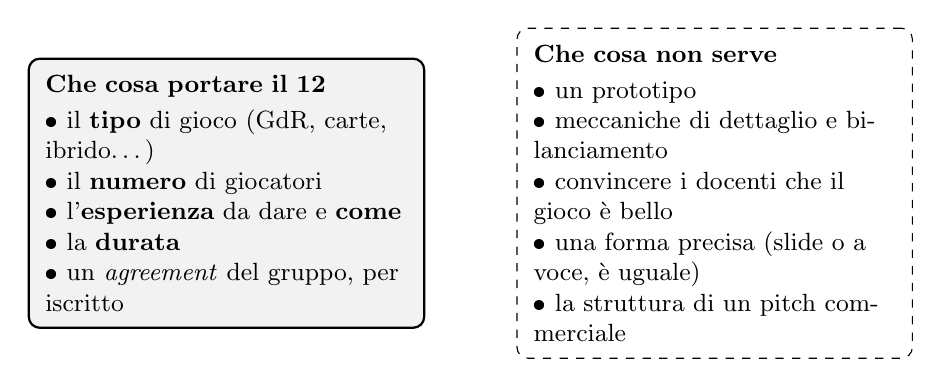
\begin{tikzpicture}[
    font=\small,
    si/.style={draw, thick, rounded corners, text width=4.6cm, align=left,
      fill=gray!10, inner sep=6pt},
    no/.style={draw, dashed, rounded corners, text width=4.6cm, align=left,
      fill=white, inner sep=6pt}
  ]
  \node[si] (a) at (0,0) {\textbf{Che cosa portare il 12}\\[2pt]
    \textbullet\ il \textbf{tipo} di gioco (GdR, carte, ibrido\ldots)\\
    \textbullet\ il \textbf{numero} di giocatori\\
    \textbullet\ l'\textbf{esperienza} da dare e \textbf{come}\\
    \textbullet\ la \textbf{durata}\\
    \textbullet\ un \emph{agreement} del gruppo, per iscritto};
  \node[no] (b) at (6.2,0) {\textbf{Che cosa non serve}\\[2pt]
    \textbullet\ un prototipo\\
    \textbullet\ meccaniche di dettaglio e bilanciamento\\
    \textbullet\ convincere i docenti che il gioco è bello\\
    \textbullet\ una forma precisa (slide o a voce, è uguale)\\
    \textbullet\ la struttura di un pitch commerciale};
\end{tikzpicture}
\caption{Il ``pitch'' del 12 ottobre come lo descrive Ruggero all'inizio della
lezione: un accordo sul \emph{che cosa}, non una vendita. Ricostruzione schematica.}
\label{a8:fig:pitch}
\end{figure}

% ---------------------------------------------------------------------
\section{Il programma: le mani nel motore}
\label{a8:sec:programma}

``Oggi, a livello logistico, vi dico cosa andiamo a fare''. Oggi è la lezione su
\textbf{Tabletop Simulator}: ``lavorare mani nel motore''. Il software va tenuto
aperto per tutta la lezione; chi non l'ha ancora installato lo installi subito (``non
è pesante, dovreste averlo pronto per tra 4 o 5 minuti''). Ci saranno domande e
momenti in cui chiedere di ``fermarmi a rispiegare una cosa'': ``fatelo, perché sono
qui apposta''.

\paragraph{Che cosa si dà per scontato.} Il software ``nasce per prototipare e
giocare'' giochi da tavolo. Ruggero dà per scontato che gli studenti l'abbiano già
usato \textbf{da giocatori} (\emph{user}, ``proprio di \emph{player}''), magari
giocando tra loro qualcosa che piace: serve ``il minimo necessario del sapersi
spostare all'interno del software'', cioè muovere la telecamera, cliccare sui menu,
sapere che cosa fanno i menu. Sono tutte cose che, come detto nel tutoraggio, ``il
tutorial di base vi spiega in 10 minuti''. Più complesso è \textbf{creare i moduli},
ed è quello che si fa oggi.

\paragraph{``Sì, ma con un asterisco''.} Tabletop Simulator è ``un software
gigantesco'' ed è impossibile coprirlo tutto in una lezione. Ruggero coprirà le
\textbf{basi} e lascerà l'ultima parte ai bisogni degli studenti: domande come ``si
può fare questa cosa qua su Tabletop Simulator?''. La risposta, ``come sempre, è quasi
sempre sì'': ``si può fare, con un asterisco: ma con un compromesso''. Il resto della
lezione spiegherà che cosa vuol dire.

Ruggero tiene il registro delle presenze in vista (``se per caso entra anche Giordano,
avvisatemi'') e condivide \textbf{tutto lo schermo}, non solo la finestra, perché
altrimenti i \emph{pop-up} del software non si vedono. Avverte che il programma, ``se
non l'avete mai aperto prima, può essere abbastanza ostile all'inizio''; ma alla fine
sarà chiaro perché è ``usatissimo nel settore'', e che ``non dovete stare 3000 ore per
saperlo usare bene''.

% ---------------------------------------------------------------------
\section{Avviare il software e creare una stanza}
\label{a8:sec:avvio}

Si lancia Tabletop Simulator da \textbf{Steam}. All'avvio il programma può proporre
un'opzione di lancio: giocare normalmente o avviare in modalità VR. Si sceglie il
gioco normale: ``è possibile usarlo con i set di realtà virtuale'', ma ``non siamo qua
per usare Tabletop in modalità VR''.

\paragraph{Il menu iniziale.} Nel menu si sente ``una musichetta fastidiosa'': si
toglie dall'ingranaggio, alla voce dei suoni, abbassando il volume del menu, ``così
magari riuscite anche a sentirmi senza impazzire''. L'icona della \textbf{lampadina}
apre il \textbf{tutorial} di base: ``io spero che voi l'abbiate già fatto. Se non
l'avete fatto, non ditemelo. Fatelo dopo la lezione senza dirmi niente, e io farò finta
che voi l'abbiate già fatto''. Poi ci sono le due voci grandi:
\begin{description}
  \item[Join] serve a unirsi a una partita che un'altra persona ha aperto; gli
        studenti dovrebbero già conoscerla, se hanno giocato con persone amiche.
  \item[Create] è quella che serve oggi: crea una partita \textbf{single player}, una
        \textbf{multiplayer} o una \textbf{hot seat}. L'\emph{hot seat} si ignora
        (``non la usa credo nessuno su questo pianeta, mai''). Il
        \emph{multiplayer} serve a creare partite con altri. Il \emph{single
        player} crea stanze in cui può entrare solo chi le crea, ed è quello che si
        usa per \textbf{costruire i moduli}.
\end{description}

\paragraph{I moduli si costruiscono in single player.} Ruggero è esplicito: ``non
create i moduli in multiplayer''. In multiplayer, del resto, solo l'\emph{host} può
crearli; ma soprattutto in single player è più comodo, perché ``la connessione
internet non vi chiederà costantemente il ping dei vostri compagni di stanza''.

All'apertura della stanza compare un \emph{pop-up} centrale, perché Tabletop
Simulator ``dà per scontato che noi vogliamo giocare qualcosa, non che vogliamo
creare un modulo''. Si chiude. Si resta con \textbf{un tavolo vuoto}, un panorama di
sfondo scelto a caso da un insieme predefinito e svariati menu. ``E a questo punto ci
dobbiamo chiedere: ok, benissimo. Cosa facciamo adesso?''.

% ---------------------------------------------------------------------
\section{``Un gioco da tavolo è un gioco su un tavolo''}
\label{a8:sec:simulatore}

Si parte ``dalle basi, proprio basi, basi''. Ruggero avverte che la lezione sarà
``piena di banalità'': frasi che suonano banalissime, ma che nell'ottica di Tabletop
Simulator ``non sono così banali''. E ripete un'informazione che era già stata messa
lì, ``nascosta, per fare \emph{foreshadowing}'', e che ripeterà ``fino allo
sfinimento'':

\begin{quote}
\textbf{Tabletop Simulator non è un software per fare videogiochi.} Non uscirete da qua
con il videogioco del vostro gioco da tavolo. Non vi serve a quello. Tabletop
Simulator, come il nome fa intuire, è un simulatore di giochi \emph{tabletop}. Vuol
dire che tutto quello che vedrete qua è \textbf{simulato fisicamente}: con un peso,
con una massa, con uno spazio, con delle collisioni.
\end{quote}

È il principio che regge tutta la lezione, e Ruggero lo riprenderà ogni volta che un
componente si comporta in modo inatteso: un mazzo che sul bordo del tavolo resta
inclinato, un cubetto che rotola giù dalla cornice di una plancia, una carta bucata
che però collide come se fosse intera. ``Questo è un simulatore di spazio fisico.
Spero che, se c'è una cosa che vi entra da oggi, è questa''. La conseguenza pratica:
i componenti di un modulo \textbf{vanno trattati come componenti fisici}, con le
stesse attenzioni che si avrebbero su un tavolo vero.

\paragraph{Approfondimento: il prototipo come simulazione.} La distinzione di Ruggero
tra \emph{simulatore} e \emph{motore} è la stessa che separa un prototipo di un gioco
da tavolo dalla sua versione digitale. Un adattamento digitale \emph{applica} le
regole al posto dei giocatori; un simulatore fisico, invece, lascia le regole ai
giocatori, come il tavolo vero, e si limita a riprodurre gli oggetti. È proprio questo
che lo rende adatto al \emph{playtest}: Schell, in \emph{The Art of Game Design},
insiste che ogni prototipo deve rispondere a una domanda precisa, e che la sua
fedeltà va scelta in funzione di quella domanda. Un prototipo su TTS risponde bene
alle domande su regole, spazio e flusso del turno, perché i giocatori devono ancora
eseguire tutto a mano, come farebbero con la scatola; risponde male, per costruzione,
alle domande che riguardano la manualità e il tatto. Il divieto degli \emph{script}
che Ruggero darà a fine lezione (sezione~\ref{a8:sec:script}) nasce dalla stessa
logica.

% ---------------------------------------------------------------------
\section{Il tavolo e la table presence}
\label{a8:sec:tavoli}

Nel menu in alto c'è la voce \textbf{Oggetti}, con quattro sottomenu:
\textbf{componenti}, \textbf{tavoli}, \textbf{background} e \textbf{oggetti
salvati}. Si parte dal tavolo.

\paragraph{Non tutti i giochi stanno su tutti i tavoli.} Nella vita reale, ``nella vita
di tutti i giorni, fisicamente'', alcuni giochi da tavolo su alcuni tavoli non si
possono giocare. Su un tavolino da caffè ``non ci sta probabilmente tutto
\emph{Twilight Imperium}''; sui tavolini del treno non ci si gioca un
\emph{eurogame}, ``perché il tavolo è più piccolo''. Allo stesso modo, quando si pensa
alla \textbf{table presence} del proprio gioco, cioè allo \textbf{spazio che occupa sul
tavolo}, la scelta non è casuale: non lo è nel mondo reale e non lo è su Tabletop
Simulator, perché lo spazio fisico è limitato: ``le cose che non sono sul tavolo
cadono dal tavolo''.

Il software offre \textbf{dieci tavoli}. Ruggero li mostra uno per uno
(tabella~\ref{a8:tab:tavoli}), guardando ogni volta due cose: quanti \textbf{posti}
ha e com'è fatto il \textbf{bordo}.

\paragraph{Le mani sono i posti a sedere.} Per contare i posti si usa, nel menu a
sinistra, la voce \textbf{Zone}, sottovoce \textbf{Hands}: mostra le \textbf{mani} di
carte, cioè le persone al tavolo. ``La \emph{hand} è in tutto e per tutto quanti
posti a sedere ci sono''. Se il tavolo ha quattro mani, ``questo gioco non può tenere
fisicamente più di quattro persone''; se si progetta un gioco da 6--8 persone, quel
tavolo ``già non va bene''.

\paragraph{Perché guardare i bordi.} ``So che vi sembra apparentemente inutile questa
informazione'', ma sopra il tavolo ci saranno dei componenti, e i componenti sono
oggetti fisici. Un bordo tridimensionale impedisce di tenere a bordo tavolo, ``belle
piatte, tranquille'', le plance dei giocatori; un rilievo al centro impedisce di
appoggiarvi piatta una plancia o un tabellone, perché ``questa salita qua è una
salita fisica che andrà a impattare i vostri componenti''.

\begin{table}[htbp]
\centering
\small
\begin{tabular}{@{}p{2.7cm}p{1.2cm}p{8.6cm}@{}}
\toprule
\textbf{Tavolo} & \textbf{Posti} & \textbf{Che cosa ne dice Ruggero} \\
\midrule
Square & 4 & piccolo, ``piccolino''; quattro persone ``strettine'' \\
Hexagon & 6 & un posto per lato, forma ``bizzarra''; \textbf{bordi
tridimensionali}: niente plance piatte a bordo tavolo \\
Octagon & 8 & come l'esagonale, con otto posti \\
Round & 8 & bordi molto meno marcati, ma al centro un \textbf{cerchio di vetro in
rilievo}: niente tabellone piatto al centro \\
Poker & -- & ``non vi servirà, a meno che non dobbiate fare poker'' \\
Rectangle & 8 & ``belli larghi''; bordi scanalati, ma superficie ampia: va bene per
``la maggior parte dei giochi pubblicati oggi'' \\
Round Glass & 8 & rotondo, grande, di vetro semitrasparente, con le gambe visibili
sotto, ``in stile Escher'': ``il tavolo peggiore di tutti. Non usatelo mai'' \\
Custom Rectangle & 8 & accetta un'immagine come superficie; il più grande; non se ne
sceglie la dimensione; l'immagine viene \textbf{stirata} \\
Custom Square & 8 & accetta un'immagine; gambe metalliche riflettenti; ``sembra
piccolo, ma è gigante''; nessun bordo strano \\
None & -- & nessun tavolo: i componenti ``cadono all'infinito in questo pozzo senza
fondo''. È l'opzione preferita di Ruggero, per un motivo che spiegherà dopo
(sezione~\ref{a8:sec:moduli}) \\
\bottomrule
\end{tabular}
\caption{I dieci tavoli di Tabletop Simulator come li presenta Ruggero. I nomi sono
quelli dell'interfaccia; i posti sono le \emph{hands} visibili nella voce
\emph{Zone}\protect\footnotemark.}
\label{a8:tab:tavoli}
\end{table}
\footnotetext{Per il tavolo da poker e per quello di vetro la trascrizione non riporta
il numero di posti (per il secondo dice solo ``per otto persone''). Il nome
``Round Glass'' per il tavolo di vetro è quello dell'interfaccia, che Ruggero non
pronuncia: lo descrive soltanto.}

\paragraph{Perché il software è fatto così.} Davanti al tavolo rotondo con il rilievo
al centro, la domanda viene da sé: perché qualcuno l'ha fatto? La risposta di Ruggero,
che tornerà molte volte nella lezione, è un misto di esasperazione e di affetto:
``perché sono pazzi'', ``è un miracolo che esista''. Chi ha creato il software ``non
sapeva cosa stava facendo''; oggi ci si ritrovano ``delle scelte vestigiali di gente
fulminata di anni fa che, contro la loro volontà, hanno purtroppo creato il software
di riferimento del settore, che è quello che tutti usano adesso''. E con queste scelte
``dobbiamo venire a patti''.

\paragraph{La scelta della lezione.} Per il prototipo dimostrativo Ruggero sceglie il
\textbf{tavolo quadrato custom} con una texture di legno: ``abbiamo un gioco piccolo,
magari un \emph{fillerino} per quattro persone, perfetto''. Sul tavolo senza tavolo
(\emph{None}) promette di tornare: ``ve lo spiego dopo, perché potrebbe essere
interessante''.

% ---------------------------------------------------------------------
\section{Caricare un'immagine: file locale e cloud}
\label{a8:sec:caricare}

Il tavolo \emph{Custom Rectangle}, appena selezionato, apre un \emph{pop-up} che chiede
un'\textbf{immagine}. È il primo incontro con una procedura che si ripeterà per quasi
ogni componente custom, e Ruggero ne fissa subito le due regole.

\paragraph{Regola 1: mai un URL, sempre un file.} Su Tabletop Simulator un oggetto
custom si può creare in due modi: dandogli l'\textbf{URL} di un'immagine online o
caricando un'immagine dal proprio computer (\textbf{Browse Local Files}). ``Il mio
consiglio personale è: non dategli mai un URL immagine'', perché se qualcuno, per
qualunque motivo, toglie quell'immagine dal suo indirizzo, ``il vostro modulo crolla''.
Se online c'è un'immagine che piace, la si \textbf{scarica} e la si ricarica dalla
propria cartella.

\paragraph{Regola 2: mai in locale, sempre in cloud.} Quando si carica un file, il
software chiede se caricarlo \textbf{in cloud} o \textbf{in locale}. ``Non caricate mai
niente del vostro modulo in locale'': un modulo con immagini locali non si può usare
in multiplayer, funziona solo sul proprio computer, e questo ``sconfigge un po'
l'obiettivo'' di farlo vedere, per esempio, a un \emph{publisher} esterno. Si carica
quindi in cloud, gli si può dare un nome, si aspetta che ``finisca di circolare questo
cerchiettino'' e si fa \textbf{Import}.

\paragraph{Le proporzioni.} Ruggero carica prima una texture di legno, poi un
tabellone più elaborato\footnote{La trascrizione descrive l'immagine come ``le
influenze moderne nella scena del Nord di Clarp'': con ogni probabilità è la
copertina o una pagina di un lavoro sul LARP nordico, usata a caso come esempio; il
contenuto dell'immagine non ha importanza.}: sul tavolo si può avere un tabellone,
uno schema, delle zone, ``già qualcosa di meccanico''. Ma la dimensione del tavolo non
si può definire: è il tavolo più grande che c'è, e l'immagine vi si adatta. Con una
texture verticale (una ``A'' arancione), il software ``la streccia come se non ci fosse
un domani'', e in più crea una luce arancione in faccia ``che sembra uscita da un film
sci-fi''. Quindi: \textbf{occhio alle proporzioni} delle immagini. Di solito il tavolo
si usa \textbf{con una texture}, e i tabelloni si mettono \textbf{a parte}, senza
caricarli direttamente sul tavolo, perché il tavolo li distorce.

% ---------------------------------------------------------------------
\section{Lo sfondo cambia la luce}
\label{a8:sec:sfondi}

Scelto il tavolo, Ruggero fa notare che la scena è buia: il suo sfondo è ``sera al
crepuscolo'', in mezzo a un prato, ``con tutto il problema di illuminazione che ne
deriva''. Il motivo è che Tabletop Simulator simula la \emph{skybox}, l'ambiente
attorno al tavolo. Dalla voce \textbf{Background} si sceglie lo sfondo: ``in questo
momento abbiamo il \emph{sunset}'', poi c'è il \emph{tunnel}, e così via.

Cambiando sfondo, Ruggero chiede di guardare il tavolo: che cosa succede? Uno studente
risponde: cambia il riflesso. Sì, e cambiano anche il livello di illuminazione e
l'angolazione. Non solo sulle gambe metalliche, che riflettono, ma anche sulla texture
di legno, che non è metallica: ingrandita, mostra colori ``più freddi, più caldi in base
a dove sono''. La luce, in Tabletop Simulator, arriva \textbf{da tre direzioni}:
\textbf{dall'alto}, \textbf{dall'orizzonte} e come \textbf{riflesso dal basso}. ``Stiamo
nel tecnico, mi rendo conto''; per ora il prato va benissimo. La questione tornerà con
il PDF, quando si vedrà che lo sfondo può rendere illeggibile un componente
(sezione~\ref{a8:sec:luce}).

% ---------------------------------------------------------------------
\section{I componenti: importare o creare?}
\label{a8:sec:componenti}

Abbiamo il tavolo, abbiamo lo sfondo, ``fantastico''. Ma mancano i componenti per
giocare. ``Vi sorprenderà sapere'' che dalla voce \textbf{Oggetti}, sottovoce
\textbf{Componenti}, si possono mettere dei componenti sul tavolo. I componenti sono
divisi in \textbf{16 categorie}, alcune più personalizzabili di altre. E l'approccio da
avere con questo software, per ogni pezzo del proprio gioco, è una domanda in due
tempi:

\begin{quote}
Devo importare un componente nel mio gioco? Ho qualcosa che mi può servire
\textbf{che già esiste}? O devo \textbf{crearlo da zero}?
\end{quote}

Ruggero passa quindi prima in rassegna i componenti ``più o meno standardizzati'' e il
modo di adattarli, e solo alla fine i componenti \emph{ad hoc}, i \textbf{custom}.

\subsection{Blocchi e cubetti}
\label{a8:sec:cubetti}

Nella categoria \textbf{Blocchi} ci sono un quadrato, un rettangolo e un triangolo; si
trascinano sul tavolo e si nota che sono \textbf{3D}. Rettangoli e triangoli per ora
non servono: si tengono i \textbf{cubetti}, una risorsa ``usatissima'' nei giochi da
tavolo. Ruggero chiede un esempio di gioco con i cubetti: gli studenti citano
\emph{Terraforming Mars} e \emph{Azul}\footnote{``Asol'' e ``terraform in Mars'' (poi
``terraform in Mark'') nella trascrizione. Ruggero aggiunge che in \emph{Azul} ci sono
``i cubetti neri per il contafonti'': il dettaglio non è ricostruibile con certezza
dalla trascrizione.}.

\paragraph{Ricolorare.} Il problema è che il cubetto è rosso, e nei giochi citati i
cubetti hanno altri colori. ``Ci può andare bene come forma, ma non come colore''. Per
ricolorarlo: \textbf{tasto destro}, \textbf{Color Tint}, e si sceglie il colore con la
classica barra di tonalità e saturazione, ``inclusa la semitrasparenza'': la barra in
fondo regola la trasparenza, e un cubetto blu con la barra abbassata diventa
semitrasparente. Un cubetto ``di grano'' si fa giallo, e così via.

\paragraph{Copiare.} Mentre si creano i moduli si possono usare \texttt{Ctrl+C} e
\texttt{Ctrl+V}: ``io posso copiarmi questi cubetti quanti ne voglio''.

\paragraph{Ridimensionare.} Un componente si può ingrandire o rimpicciolire dalla
tastiera, con i tasti \texttt{+} e \texttt{-}: per esempio un cubo più grande degli
altri, che valga tre o cinque risorse.

\subsection{Le dimensioni reali}
\label{a8:sec:misurare}

Il ridimensionamento serve per tutti i componenti, e qui Ruggero chiede di
``prepararsi psicologicamente'': quando si fanno moduli su Tabletop Simulator,
\textbf{è buona pratica mantenere le dimensioni e le proporzioni reali dei
componenti}. Ma come si sa quanto è grande un cubo? ``Può essere 10 cm, come 150, che
ne sappiamo''.

\paragraph{Lo strumento Linea.} Nel menu a sinistra c'è lo strumento \textbf{Linea}
(il righello). Nelle sue impostazioni si sceglie l'\textbf{unità}: Ruggero consiglia i
\textbf{centimetri} e la modalità 2D\footnote{La trascrizione rende le impostazioni
consigliate come ``2D free edge no log''; Ruggero dice di non volerle spiegare ``per
limiti di tempo'' e che ``centimetri, 2D'' è quello che serve. La forma esatta delle
altre voci non è ricostruibile dalla trascrizione.}. Con lo strumento si tira una
linea e il software scrive la misura sul bordo: il lato del cubo è ``più o meno 8
cm''.

\paragraph{Misurare dall'alto.} Per misurare con precisione si cambia prospettiva con
il tasto \texttt{P}, passando alla vista \textbf{dall'alto} (\emph{top-down}): senza
il problema del 3D si misura ``da un angolo all'altro''. Il lato risulta di 7 cm.
Se il cubetto dev'essere di 20 mm, lo si ridimensiona con \texttt{+} e \texttt{-}
finché la misura non è ``più o meno 2 cm''.

\paragraph{Una domanda di chiarimento.} Uno studente non ha capito: il cubo è stato
ridimensionato con la linea? No: il cubo si ridimensiona \textbf{con i tasti più e
meno}; la linea \textbf{misura} soltanto. Il tasto \texttt{Tab}, premuto una volta,
mette le freccette per indicare le cose; \textbf{tenuto premuto}, mostra la linea di
misura. Un'altra studentessa non ha capito come cambiare prospettiva: tasto \texttt{P},
``di prospettiva'', che passa tra prima persona, terza persona e vista dall'alto. Sono
cose che il tutorial dovrebbe aver già insegnato; in ogni caso, con il tasto
\texttt{Esc} si apre l'\textbf{Help}, con tutte le scorciatoie del software. Anche
spostare più componenti insieme e interagire con i componenti sono cose del tutorial.

\begin{figure}[htbp]
\centering
\begin{tikzpicture}[
    font=\small,
    passo/.style={draw, thick, rounded corners, text width=2.6cm, align=center,
      minimum height=1.3cm, fill=gray!10},
    freccia/.style={-{Stealth[length=2.5mm]}, thick}
  ]
  \node[passo] (a) at (0,0) {Linea: unità in \textbf{cm}, modalità \textbf{2D}};
  \node[passo] (b) at (3.3,0) {\texttt{P}: vista \textbf{dall'alto}};
  \node[passo] (c) at (6.6,0) {\texttt{Tab} tenuto premuto: \textbf{misura}};
  \node[passo] (d) at (9.9,0) {\texttt{+} / \texttt{-}: \textbf{scala} fino alla misura reale};
  \draw[freccia] (a) -- (b);
  \draw[freccia] (b) -- (c);
  \draw[freccia] (c) -- (d);
  \draw[freccia, dashed] (d.south) to[bend left=25] node[below, font=\footnotesize]
    {si rimisura finché non torna} (c.south);
\end{tikzpicture}
\caption{Come portare un componente alle sue dimensioni reali, secondo la procedura
mostrata da Ruggero: nell'esempio, un cubetto da 7 cm ridotto a 2 cm.}
\label{a8:fig:misurare}
\end{figure}

% ---------------------------------------------------------------------
\section{Le plance}
\label{a8:sec:plance}

La categoria \textbf{Board} contiene le \textbf{plance}: backgammon, scacchi o dama,
un'altra versione della scacchiera, dama cinese, Go, Reversi. ``La domanda però è:
perché ci sono?''. Il proprio gioco sarà sicuramente diverso da questi: quello che
serve, di solito, è la \textbf{Custom Board}, che chiede, ``indovinate un po''',
un'immagine, come il tavolo custom.

\paragraph{Bloccare la plancia.} La plancia si può spostare; con il tasto \texttt{L},
di \emph{lock}, la si \textbf{blocca}, in modo che cliccandoci sopra, anche per
sbaglio, non si sposti più. ``Questa è una buona pratica, perché noi non vogliamo che
qualcuno sposti il tabellone con tutte le cose sopra''.

\paragraph{La plancia si adatta all'immagine.} Uno studente nota che la plancia ha
cambiato dimensione da sola. Esatto: \textbf{al contrario del tavolo}, che adatta
l'immagine alla cornice (stirandola), \textbf{la board adatta la cornice
all'immagine}. Un'immagine alta dà una plancia stretta e alta; cambiandola (tasto
destro, \textbf{Custom}) con la texture del tavolo, la plancia si allunga dall'altro
lato. Ne segue una regola per i tabelloni: importarli \textbf{nelle proporzioni che
devono avere nella realtà}.

\paragraph{Il problema della cornice.} ``Ma adesso ti faccio vedere un'altra cosa''.
La plancia custom ha un \textbf{bordo di legno} in rilievo, ``nello stile delle vecchie
scacchiere''. E siccome i componenti sono 3D, un cubo appoggiato sul bordo
\textbf{rotola giù}. ``Quanti board game recenti avete visto con le plance che hanno la
cornice in legno alta due centimetri?''. Nessuno, risponde uno studente; ``forse una
versione super antica degli scacchi di mio nonno''. ``Esatto, perché è una roba da
fuori di testa'': nessuno mette una cornice di legno su un tabellone che costa 200
euro. La cornice non si può togliere. La soluzione arriverà più avanti
(sezione~\ref{a8:sec:tabellone}); per ora: ``tenetevi in background l'informazione''.

% ---------------------------------------------------------------------
\section{Le carte standard}
\label{a8:sec:carte-std}

La categoria \textbf{Carte} contiene: uno \emph{standard deck}, un \emph{custom deck},
una \emph{custom card}, una carta a caso (``randomicamente ci pesca una carta a
caso''), un \textbf{Jolly} (perché il mazzo standard è ``il classico deck da poker
normale di 52 carte'' e non ha i Jolly) e alcuni mazzi creati dagli autori di Tabletop
Simulator per un loro gioco, ``che non servono a niente di niente'': ``li lanciamo nel
sole''.

Come si interagisce con un mazzo (spostarlo, pescare, rivelare, pescare nella propria
mano) lo insegna il tutorial. Quello che importa sapere è che il mazzo \textbf{ha una
proprietà fisica}: la carta singola è più leggera del resto, il mazzo è
tridimensionale, e un mazzo appoggiato sul bordo del tavolo resta \textbf{inclinato},
tanto che si può vedere che cosa c'è sotto. ``Questo è un simulatore di spazio fisico.
Spero che, se c'è una cosa che vi entra da oggi, è questa''. I componenti ``vanno
trattati come se fossero componenti fisici''.

E se il gioco usa un mazzo di carte evento personalizzate? ``Ve lo spiego dopo'': prima
i componenti standard e come adattarli, ``e poi passiamo per ultimo ai componenti
\emph{ad hoc} vostri'' (sezione~\ref{a8:sec:mazzo}).

% ---------------------------------------------------------------------
\section{Dama, scacchi, dadi e figurine}
\label{a8:sec:dadi}

\paragraph{Dama e scacchi.} La quarta categoria sono i pezzi della \textbf{dama}, ``e
qui davvero abbiamo la follia di Tabletop Simulator'': c'è di nuovo la plancia,
identica a quella della categoria precedente, presente quindi in due categorie. Negli
\textbf{scacchi} ci sono pezzi metallici o di legno; ``se volete dei riflessi
ambientali, quelli di metallo sono perfetti''. Ma la domanda è sempre: servono?
Trattandosi di prototipi, se serve un pedone, ``nessuno si scandalizza se prendete un
pedoncino così e magari lo colorate, che so, rosso''.

\paragraph{I dadi.} Nella categoria \textbf{Dadi} ci sono dadi metallici e di plastica,
già colorati: d4, d6, d8, d10, d12 e d20, più altre versioni (per esempio d6 colorati
con gli angoli arrotondati). Si possono ricolorare e ingrandire: ``mi servono da 20,
ma blu''; lo si ricolora, lo si fa più grosso degli altri, e si tira come gli altri.
Ma attenzione: \textbf{ricolorare un componente non colora tutto}. Un dado bianco
colorato di giallo mantiene i \textbf{pallini} neri; un dado metallizzato colorato di
giallo ha i pallini bianchi, ed è \textbf{illeggibile}; un dado colorato di nero ``fa
schifo'', uno colorato di bianco è ``completamente illeggibile''. Quindi: attenzione a
quali componenti si scelgono come base.

\paragraph{Le figurine.} Nella categoria \textbf{Figurine} ci sono gli \emph{standee}
(le sagome in piedi) e le figurine metalliche, ``i classici omini di piombo'', che non
servono. Serve il \textbf{custom standee}, che chiede un'immagine di \textbf{fronte} e
una di \textbf{retro}. Ruggero vi mette la sua ``A'' davanti e dietro, ``ed ecco il
nostro standee''. Può essere un personaggio anche con la trasparenza: un PNG ritagliato
mantiene lo sfondo trasparente. Per avere un'immagine più grande mantenendo la base
piccola si usa il fattore di \textbf{scala}: con 2, l'immagine raddoppia e la base
resta piccola. ``Mi rendo conto che può essere estremamente noioso per ora questo
software''; tra poco arrivano ``le cose custom per davvero''.

% ---------------------------------------------------------------------
\section{Go, biglie, miscellanea}
\label{a8:sec:misc}

Ruggero passa ``velocissimamente'' sul resto.

\paragraph{Le pedine del Go.} Le pietre del Go ``possono essere come risorse'': si
vogliono risorse che siano sassolini, anziché cubetti? Benissimo. Colorate di azzurro
e rese semitrasparenti, diventano ``delle gocce d'acqua''.

\paragraph{Le biglie e i giochi di destrezza.} Le \textbf{biglie} sono biglie,
``letteralmente, con tutta la fisica che ne comporta'': su una superficie piana
continuano a rotolare. A che cosa servono? Ai \textbf{dexterity game}, i giochi di
destrezza, che si possono fare anche qui. La dimostrazione: Ruggero prende un
componente, lo mette sul tavolo e lo blocca; poi usa lo strumento \textbf{Flick} (il
``colpetto'' con il dito) sulla biglia, che va a sbatterci contro. ``Voilà! È un
simulatore fisico questo software''.

\paragraph{La miscellanea.} ``Dentro la miscellanea abbiamo tante cose bizzarre''.
\begin{itemize}
  \item Una \textbf{ciotola}: come componente non serve, ma bloccata sul tavolo e
        riempita di cubetti dà ``improvvisamente una \emph{table presence}
        diversa''.
  \item Una \textbf{moneta}, che lanciata dice testa o croce.
  \item Le pedine del \textbf{Reversi}, a due facce, una bianca e una nera: un
        \emph{token} a due lati già pronto.
  \item Pezzi del \textbf{domino}, tessere del \textbf{Mahjong}\footnote{``Testa del
        Maggiog'' nella trascrizione.}, altri dischetti, tutti ricolorabili, da
        usare come risorse.
  \item Un insieme di componenti dei designer del software\footnote{La trascrizione
        lo chiama ``P-Spec''; il nome della categoria non è ricostruibile con
        certezza.}: ``se vi servono, bene; se no, il mio sospetto è che non vi
        serviranno mai''.
  \item I \textbf{Player Pawn}, i classici pedoni di plastica, in \textbf{nove
        colori}. Perché nove versioni, se si possono ricolorare? ``Perché sono pazzi, i
        designer: non ci hanno pensato''. Ricolorateli come volete.
\end{itemize}

\paragraph{I colori dei giocatori.} C'è però una ragione per ricolorare con criterio.
Nel selettore dei colori, la colonna a destra contiene esattamente i \textbf{colori dei
giocatori}, cioè i colori delle mani attorno al tavolo\footnote{Ruggero dice prima
``questi 16 colori'' e poi ``esattamente i 12 colori player''; la trascrizione non
permette di stabilire quale dei due numeri sia quello inteso.}. Se si vuole un codice
colore preciso, legato al giocatore, si sceglie da lì: ``fammelo di questo arancione''
dà esattamente l'arancione del giocatore arancione.

\paragraph{Fiches e kit da GdR.} Poi le \textbf{fiches} da poker, ``classiche fiches
da casinò''; e il \textbf{RPG Kit}: miniature su miniature da \emph{dungeon crawler},
maghi, guerrieri, mostri, creature. ``Si muovono da sole queste'' (sono animate), ``un
po' anni Duemila, ma oh: per un prototipo su TTS, chi se ne frega?''.

\paragraph{Le cose ``fulminate''.} Infine la categoria preferita di Ruggero: ``le cose
così fulminate che mi fanno chiedere: ma perché, perché, perché hanno messo queste
cose qua? Non avremo mai una risposta''.
\begin{itemize}
  \item Una \textbf{Notecard}: un foglietto su cui si scrive con il tasto destro,
        compilando \textbf{nome} (il titolo) e \textbf{descrizione}. Si chiamano
        \textbf{index card}, ``usatissime per i giochi di ruolo in ambito americano,
        il \emph{tabletop} RPG specialmente''. Una studentessa si è persa: come si
        scrive? Tasto destro, e in fondo ci sono i due campi, nome e descrizione; si
        può andare a capo e mettere più righe; il testo ``non è in tempo reale'', si
        aggiorna solo quando si esce dal menu.
  \item Un \textbf{lettore MP3}: ``che devo dirvi? C'è un lettore MP3. Se volete
        giocare con la musica, ce l'abbiamo''. (Ruggero verifica che la classe senta
        l'audio del suo computer: ``vi voglio far soffrire per davvero''.)
  \item Un \textbf{contatore}, che si può far salire, scendere, azzerare, o in cui si
        scrivono direttamente i numeri.
  \item Un \textbf{tablet}, ``letteralmente un tablet'': ci si può aprire YouTube e
        guardare video. ``È un tablet, ragà, è un tablet. Non so che dirvi''.
  \item Una \textbf{sveglia} e una \textbf{calcolatrice}.
\end{itemize}

% ---------------------------------------------------------------------
\section{I sacchetti}
\label{a8:sec:sacchetti}

Nella miscellanea ci sono finalmente ``le due cose che ci servono per davvero'': il
\textbf{sacchetto infinito} e il \textbf{sacchetto}.

\paragraph{Il sacchetto infinito.} Parte vuoto e rende infinito qualunque cosa gli si
metta dentro: con un dado blu diventa un sacchetto infinito di dadi blu. Si può
ricolorare e si può azzerare (tasto destro, \textbf{Reset}) per farne, per esempio, un
sacchetto di dadi rossi. Ma Ruggero fa una richiesta precisa: \textbf{nei moduli per
questo corso non si usa il sacchetto infinito}, perché ``a livello produttivo io vi
chiederò quanti componenti avete, e infiniti non è un numero che è possibile stampare
nella realtà''. Per comodità è utilissimo, ``ma non è questo il momento''.

\paragraph{Il sacchetto normale.} Parte vuoto (passandoci sopra con il mouse si legge
zero) e ci si mette dentro qualunque cosa. Ruggero colora tre cubetti di giallo, rosso
e blu e li mette nel sacchetto; poi, con il tasto destro, decide \textbf{in che ordine}
il sacchetto restituisce gli oggetti (figura~\ref{a8:fig:sacchetto}):
\begin{description}
  \item[LIFO] (\emph{last in, first out}): l'ultimo oggetto messo è il primo a
        uscire. Messi blu, rosso, giallo, escono giallo, rosso, blu.
  \item[FIFO] (\emph{first in, first out}): il primo messo è il primo a uscire.
        Messi blu, rosso, giallo, escono blu, rosso, giallo.
  \item[Random]: ``è random''.
\end{description}
``Chiaramente non siamo persone fulminate'': un sacchetto, nella realtà, si comporta in
modo casuale, e quindi si mette \textbf{Random}. Nella prova, blu, rosso, giallo escono
giallo, rosso, blu.

\paragraph{Guardare dentro.} Per vedere che cosa c'è nel sacchetto: tasto destro,
\textbf{Search}. La stessa funzione si usa sui \textbf{mazzi}, per vedere le carte
rimaste.

\begin{figure}[htbp]
\centering
\begin{tikzpicture}[
    font=\small,
    cubo/.style={draw, minimum size=0.55cm, inner sep=0pt},
    etich/.style={font=\small\bfseries, anchor=east},
    freccia/.style={-{Stealth[length=2mm]}, thick}
  ]
  % ingresso
  \node[font=\footnotesize] at (0.9,1.9) {si inserisce};
  \node[cubo, fill=blue!40] at (0,1.3) {B};
  \node[cubo, fill=red!40] at (0.9,1.3) {R};
  \node[cubo, fill=yellow!50] at (1.8,1.3) {G};
  \draw[freccia] (2.3,1.3) -- (3.3,1.3);
  \node[draw, thick, rounded corners=6pt, minimum width=1.5cm, minimum height=1.2cm,
    align=center, font=\footnotesize] at (4.2,1.3) {sacchetto};
  % uscite
  \node[etich] at (7.2,2.2) {LIFO};
  \node[cubo, fill=yellow!50] at (7.7,2.2) {G};
  \node[cubo, fill=red!40] at (8.4,2.2) {R};
  \node[cubo, fill=blue!40] at (9.1,2.2) {B};
  \node[etich] at (7.2,1.3) {FIFO};
  \node[cubo, fill=blue!40] at (7.7,1.3) {B};
  \node[cubo, fill=red!40] at (8.4,1.3) {R};
  \node[cubo, fill=yellow!50] at (9.1,1.3) {G};
  \node[etich] at (7.2,0.4) {Random};
  \node[cubo] at (7.7,0.4) {?};
  \node[cubo] at (8.4,0.4) {?};
  \node[cubo] at (9.1,0.4) {?};
  \draw[freccia] (5.1,1.3) -- (5.5,2.2);
  \draw[freccia] (5.1,1.3) -- (5.5,1.3);
  \draw[freccia] (5.1,1.3) -- (5.5,0.4);
  \node[font=\footnotesize] at (8.4,2.8) {ordine di uscita};
\end{tikzpicture}
\caption{Le tre modalità del sacchetto, con l'esempio di Ruggero: tre cubetti
inseriti nell'ordine blu, rosso, giallo (B, R, G). Per un gioco da tavolo si usa
\emph{Random}, che è il comportamento di un sacchetto reale.}
\label{a8:fig:sacchetto}
\end{figure}

\paragraph{Approfondimento: il prototipo e la produzione.} La richiesta di non usare il
sacchetto infinito anticipa un tema che il corso affronterà con la lezione sulla
produzione: un gioco analogico è anche una \textbf{distinta dei componenti}, e ogni
componente ha un costo. Un modulo che usa scorte infinite nasconde al designer la
domanda ``quanti me ne servono davvero?'', che in un gioco stampato ha sempre una
risposta. Lo stesso vale per i cubetti copiati a volontà con \texttt{Ctrl+V}: comodi
per costruire, ma da contare prima di consegnare.

% ---------------------------------------------------------------------
\section{I componenti custom}
\label{a8:sec:custom}

``Allora, adesso arriviamo alla parte più incubo di tutte, che è la parte custom''. La
categoria \textbf{Custom} raduna tutte le opzioni personalizzabili, comprese quelle già
viste (la plancia, le figurine). Sono dieci (tabella~\ref{a8:tab:custom}).

\begin{table}[htbp]
\centering
\small
\begin{tabular}{@{}p{2.6cm}p{10.0cm}@{}}
\toprule
\textbf{Componente} & \textbf{A che cosa serve e che cosa ne dice Ruggero} \\
\midrule
Custom Board & una plancia da un'immagine; la cornice si adatta all'immagine, ma ha
il bordo di legno (sezione~\ref{a8:sec:plance}) \\
Custom Figurine & lo \emph{standee} con fronte e retro (sezione~\ref{a8:sec:dadi}) \\
Custom PDF & il \textbf{regolamento} del gioco, consultabile sul tavolo \\
Custom Token & un gettone con \textbf{forma libera} (gestisce la trasparenza e la
collisione), colorabile, impilabile; il retro è specchiato \\
Custom Tile & una tessera di \textbf{forma regolare} (quadrata, esagonale, circolare,
arrotondata) con fronte e retro corretti \\
Custom Deck & un \textbf{mazzo} di carte da una griglia di immagini: ``la parte più
difficile di tutte'' \\
Custom Card & una carta singola, fronte e retro \\
Custom Dice & un dado con le facce personalizzate, da un \emph{template} \\
Custom Model & un modello 3D (mesh, texture, collider): non si vede a lezione \\
Custom AssetBundle & pacchetti di modelli 3D, per esempio miniature: non si vede a
lezione \\
\bottomrule
\end{tabular}
\caption{I dieci componenti della categoria \emph{Custom}, come Ruggero li elenca
(``board, tile, token, figurine, deck, card, dice, model, asset bundle, PDF''). Modelli
3D e asset bundle in fase di prototipo sono fortemente sconsigliati.}
\label{a8:tab:custom}
\end{table}

% ---------------------------------------------------------------------
\section{Il PDF del regolamento e la luce}
\label{a8:sec:luce}

\paragraph{Caricare un PDF.} Il \textbf{Custom PDF} chiede di caricare un PDF. Ruggero
ne carica uno a caso, ``così a caso'': un PDF sul \emph{framework} DPE\footnote{``DPA
Framework'' nella trascrizione; con ogni probabilità il materiale sul framework DPE
(\emph{Design, Play, Experience}) visto nelle lezioni precedenti.}. ``Sempre
aspettare che finisca questa rondella blu, se no TTS impazzisce''. Il PDF appare sul
tavolo: è \textbf{molto piccolo} ed è \textbf{molto bianco}, quasi illeggibile, perché
l'illuminazione dello sfondo ``fa schifo''. Ed ecco il punto chiave sugli sfondi,
``lasciato in sospeso'' fino ad ora: cambiando lo sfondo cambia tutto. Ma magari non si
vuole giocare ``con le vibes di un pub di fumatori incalliti''.

\paragraph{Uno sfondo da un pixel.} Nel menu degli sfondi c'è un'opzione che Ruggero
aveva taciuto apposta: \textbf{Custom}, che permette di scegliere uno sfondo proprio.
Tabletop Simulator usa per gli sfondi panorami HDRI da $4000\times2000$ pixel, in un
formato specifico; ``ma non ce ne frega niente, perché in realtà noi possiamo fregare il
sistema'': come sfondo si può dare un'immagine di \textbf{un pixel per un pixel},
monocromatica, e si ottiene uno sfondo monocromatico attorno al tavolo. Ruggero ne ha
già preparati alcuni: dal menu \textbf{Modding}, alla voce \textbf{Cloud Manager}, si
vede tutto quello che si è caricato in cloud (``utile anche a voi per sapere cosa avete
caricato''), e lui ha una cartella di immagini utili con, tra l'altro, uno sfondo nero
da un pixel, ``leggerissimo da caricare''. Copiato e incollato nel \emph{Custom
Background}, il tavolo si ritrova ``in un nulla cosmico''. Ma la luce non cambia
ancora: è ancora quella dello sfondo precedente.

\paragraph{Le impostazioni di luce.} Dal menu \textbf{Options} si apre la voce
\textbf{Lighting}. La prima cosa da fare è \textbf{slegare la luce dallo sfondo}
(c'è una spunta apposta) e scegliere il \textbf{gradiente}: la visibilità migliora
subito. Poi Ruggero va ``voce per voce'' (tabella~\ref{a8:tab:luce}): ``so che vi
sembra complessa questa roba qui, ma non vi servirà sapere tutto''.

\begin{table}[htbp]
\centering
\small
\begin{tabular}{@{}p{3.4cm}p{9.2cm}@{}}
\toprule
\textbf{Voce} & \textbf{Che cosa fa e come impostarla} \\
\midrule
Luce legata allo sfondo & da \textbf{togliere}, scegliendo il gradiente \\
Light Intensity & la luce \textbf{dall'alto}, verticale: alta ``brucia tutto'', bassa
``non si vede niente''; di solito verso il fondo della barra, ma non al minimo \\
Light Color & di default una luce calda, un bianco non puro: ``lasciate questa, è una
buona luce'' \\
Ambient Intensity & la luce \textbf{laterale}, dell'ambiente: cambia i bordi degli
oggetti, non la faccia superiore; va bilanciata con la precedente ``in modo che non vi
faccia sputare gli occhi'' \\
Gradient Color (Sky, Equator, Ground) & ``non toccateli'' \\
Reflection Intensity & quanto riflettono i componenti \textbf{metallici} (tavolo,
dadi, pezzi): abbassata, il tavolo di metallo ``non riflette più niente'' e un dado
metallico diventa opaco \\
LUT e voci successive & ``ignorate queste cose, per carità. Non apriamo questo vaso
di Pandora'' \\
\bottomrule
\end{tabular}
\caption{Le impostazioni di luce di Tabletop Simulator (menu \emph{Options},
\emph{Lighting}) con i consigli di Ruggero\protect\footnotemark.}
\label{a8:tab:luce}
\end{table}
\footnotetext{La trascrizione rende l'ultima voce come ``loot loot contribution'' e
``Gaston, loot''; dovrebbe trattarsi delle impostazioni della LUT (\emph{look-up
table}), la tabella di correzione del colore. Ruggero aggiunge che chi è appassionato
di grafica 3D può andare a vederle ``in privato''.}

\paragraph{Come si vede la differenza.} Per mostrare la differenza tra le due
intensità, Ruggero porta prima al massimo e poi al minimo l'\emph{ambient intensity}:
``sembrano simili, ma non lo sono''. Il trucco è guardare un cubetto giallo: cambiando
la \emph{light intensity}, i colori dei \textbf{bordi} restano uguali, perché è la luce
verticale; cambiando l'\emph{ambient intensity}, che è la luce laterale, la faccia
\textbf{superiore} resta uguale. Per la \emph{reflection intensity} Ruggero cambia
tavolo (``lasciamo stare che sono volati via 38 componenti insieme, perché il tavolo
l'ho rimpicciolito'') e mostra che cambiano solo i componenti metallici, ``dadi inclusi'':
un dado ``nato metallico'' sembra cambiare colore e diventa ``bello matte''.

\paragraph{Il regolamento sul tavolo.} Tornando al PDF: lo si sfoglia con le
freccette, lo si ingrandisce, lo si mette a schermo. ``Questo è come importiamo i
regolamenti dei nostri giochi'': se il gioco ha un regolamento in PDF, si carica con il
Custom PDF, ``pulito, liscio, limpido, lampante''.

\paragraph{Modelli e asset bundle: no.} \textbf{Custom Model} e \textbf{Custom
AssetBundle} servono a caricare modelli 3D personalizzati, per esempio miniature. Non
si vedranno a lezione e non servono in fase di prototipo: ``non solo non vi verrà
richiesto, ma vi verrà fortemente incentivato a non usarli, a meno che non abbiate
proprio un obbligo particolare''.

% ---------------------------------------------------------------------
\section{Token e tile}
\label{a8:sec:token}

\paragraph{Che cos'è un token.} ``Sapete cos'è un token?''. ``So che sembra una risposta
banale, ma ci aiuta''. Una studentessa risponde: sono ``tipo quelle monetine che
c'erano in alcuni giochi''. Sì, per esempio; ma fisicamente che cos'è? Un gettone, sì,
e di solito è qualcosa che viene \textbf{estratto da una fustella}, una
\emph{punchboard}: nei giochi da tavolo i token sono pezzi di cartone fustellato. ``Se
avete comprato un gioco da tavolo nuovo, probabilmente li avete visti: li spingete via
con le manine ed estraete questi tokenini di cartone''. Su Tabletop Simulator è la
stessa cosa, solo che non li si estrae da una fustella.

\subsection{Il Custom Token}
\label{a8:sec:custom-token}

Ruggero crea un token con un'immagine qualunque, il logo di Audacity: ``voilà, abbiamo
il nostro token''. Le sue proprietà:
\begin{itemize}
  \item ha uno \textbf{spessore}, che dalle impostazioni custom si può aumentare (al
        massimo diventa ``un bel tokenone grosso'');
  \item si ridimensiona con \texttt{+} e \texttt{-}, come gli altri componenti;
  \item può stare \textbf{in piedi} anziché coricato (\emph{Stand Up}); ``notate che è
        molto strano, vedremo dopo perché'';
  \item può essere \textbf{impilabile} (\emph{Stackable}).
\end{itemize}

\paragraph{Impilabile o no.} La dimostrazione: due copie dello stesso token, una
normale e una impilabile. I token non impilabili messi uno sopra l'altro formano una
pila ``fisicamente'', ma ciascuno si sposta isolatamente. I token impilabili, invece,
vengono \textbf{impilati e contati} da Tabletop Simulator: passando sopra la pila con
il mouse, il software dice che è di 14 token.

\paragraph{Le proporzioni.} Il token \textbf{mantiene le proporzioni} dell'immagine: un
token da un'immagine rettangolare (una ``B'') è rettangolare, non viene stirato.

\paragraph{Il difetto: il retro è specchiato.} Quando si gira il token, la ``B'' è
\textbf{al contrario}. Con un token che porta delle scritte (Ruggero ne prende uno con
una scritta) il problema è evidente: girato, la scritta è rovesciata. E nelle opzioni
di importazione non c'è modo di dire ``non flipparmi il retro al contrario'': con il
Custom Token \textbf{non si può importare un componente con fronte e retro corretti}.

\subsection{Il Custom Tile}
\label{a8:sec:tile}

Per avere un retro corretto si usa il \textbf{Custom Tile}, la \textbf{tessera}. Chiede
cose simili ma non identiche: un'immagine \textbf{top} e un'immagine \textbf{bottom},
cioè che cosa c'è davanti e che cosa c'è dietro. Ruggero crea un tile con la stessa
immagine scritta del token e lo porta alla stessa dimensione, così da confrontarli.
Le differenze:
\begin{itemize}
  \item il token ha il bordo del colore del fronte, il tile ha il bordo
        \textbf{bianco};
  \item girati, il tile \textbf{mantiene la scritta corretta};
  \item il tile può avere un \textbf{retro diverso} dal fronte;
  \item il tile ha opzioni di \textbf{forma}: quadrato, \textbf{esagonale},
        \textbf{circolare}, \textbf{rounded} (rettangolare con i bordini
        arrotondati); il token non le ha.
\end{itemize}
``E quindi la domanda è: perché mai dovrei usare un token, quando posso usare un tile?''.

\paragraph{Il colore.} La prima risposta è il colore. Colorati entrambi di giallo (poi
di blu), il \textbf{tile} colora \textbf{solo il bordo}, mentre il \textbf{token} mette
un \textbf{filtro} colorato su tutta l'immagine. Quindi, se si vogliono tre token con
la stessa immagine, uno rosso, uno giallo e uno blu, il token permette di colorarli; e
su un'immagine bianca il colore viene applicato preciso (un rettangolo bianco colorato
di bianco resta il colore di base).

\paragraph{La trasparenza.} La seconda risposta è la trasparenza. Il token permette di
creare segnalini con la \textbf{trasparenza}, cioè \textbf{forme personalizzate}; il
tile la trasparenza non la gestisce, e la stessa immagine darà sempre una tessera con lo
sfondo bianco. Da cui la regola (tabella~\ref{a8:tab:token-tile}): \textbf{forma
custom, token; forma regolare (circolare, quadrata, arrotondata), spesso è più comodo
il tile}. ``Se avete dubbi o domande, vi prego, chiedetele, perché da adesso in poi
questo software fa solo che complicarsi la vita''.

\begin{table}[htbp]
\centering
\small
\begin{tabular}{@{}p{3.6cm}p{4.4cm}p{4.4cm}@{}}
\toprule
 & \textbf{Custom Token} & \textbf{Custom Tile} \\
\midrule
Forma & libera, dalla trasparenza del PNG & regolare: quadrata, esagonale,
circolare, arrotondata \\
Trasparenza & sì & no (sfondo bianco) \\
Retro & lo stesso del fronte, \textbf{specchiato} & immagine \emph{top} e
\emph{bottom}, corretta e anche diversa \\
Colore (Color Tint) & filtro su tutta l'immagine & solo il bordo \\
Bordo & del colore del fronte & bianco \\
Altre opzioni & spessore, \emph{Stand Up}, \emph{Stackable} & spessore, forma \\
Quando usarlo & segnalini sagomati, \emph{meeple}, standee, tabelloni (con
spessore minimo) & tessere, segnalini con scritte su entrambi i lati, plance \\
\bottomrule
\end{tabular}
\caption{Token e tile a confronto, secondo la dimostrazione di Ruggero.}
\label{a8:tab:token-tile}
\end{table}

\paragraph{Le sagome di persone.} Una domanda: le sagome di persone sono immagini
trasparenti fatte a token? Sì: nel Custom Token c'è l'opzione \textbf{Stand Up}, e con
un bordo un po' più ampio si ottiene una sagoma in piedi (``dev'essere molto grosso,
questo però, capiamoci''). Se il bordo è impreciso, è un lavoro ``di finezza'' sulla
\textbf{Merge Distance}: modificandola, il software ritaglia bordi più o meno accurati
in base a che cosa vede nell'immagine.

% ---------------------------------------------------------------------
\section{Il dado custom}
\label{a8:sec:dado}

``E ora arriviamo al punto che è traumatico. Ma ci siamo''. Mancano due componenti, il
\textbf{dado custom} e il \textbf{mazzo custom}.

\paragraph{Un'immagine per sei facce?} Il \textbf{Custom Dice} chiede prima che dado
si vuole (d4, d6, d8, d10, d12, d20), poi \textbf{un'immagine}. Una sola immagine per
sei facce? Che immagine? Provando con un'immagine a caso, il software la
\textbf{spalma} su tutto il dado. ``Al che la risposta è: Tabletop Simulator, che cosa
hai bevuto stasera? Come faccio a sapere che immagine devo caricare su questo dado?''.

\paragraph{I template nascosti.} La risposta sta nei file di installazione. Da
\textbf{Steam}: tasto destro su Tabletop Simulator nella libreria, \textbf{Proprietà},
\textbf{File installati}, \textbf{Sfoglia}. Si apre la cartella del software, e qui
l'avvertenza è perentoria: ``modificare questi file fa esplodere Tabletop Simulator.
Quindi non cancellate niente, non toccate niente''. Dentro c'è la cartella
\textbf{Modding}, con \emph{Deck Builder}, \emph{Deck Templates}, \emph{Dice
Templates} e altro. Nei \textbf{Dice Templates} ci sono le \textbf{UV map} dei dadi
(``maledetti, infami''\ldots).

\paragraph{Che cos'è una UV map.} Per chi non ha mai fatto modellazione 3D, Ruggero usa
un'immagine: i cioccolatini a forma di coniglio o di Babbo Natale avvolti nella carta
metallizzata. Srotolata, la carta è un'immagine piatta, ma avvolge una forma
tridimensionale. Allo stesso modo, il template è ``la carta che va messa attorno a
questo dado'': dice dove sono, nell'immagine piatta, le facce che interessano.

\paragraph{La procedura.} Si fa \textbf{una copia} del template del d6 (``non
modificate direttamente quel file, vi prego''), la si carica così com'è, ``e bum'':
il dado custom ha le facce di un d6 normale (``a questo punto usa il dado base, che era
anche meno brutto da vedere''). Ma l'immagine si può modificare, con Photoshop, GIMP,
``ma anche Paint''. Ruggero la apre con Paint e fa ``un lavoro approssimativo, fatto
davvero male, giusto per capirci'': i numeri pari rossi, i dispari verdi. Salva,
ricarica, ``e voilà: abbiamo il nostro bel dado. Bello è un eufemismo, chiaramente.
Brutto, ma ce l'abbiamo''. Le facce si possono quindi riempire di simboli o di
qualunque altra cosa.

\paragraph{Dov'è la cartella?} Uno studente si è perso: qual è la cartella? Ruggero
ripete: libreria di Steam, tasto destro su Tabletop Simulator, Proprietà, File
installati, Sfoglia; poi \emph{Modding} e \emph{Dice Templates}. ``Lo so, è brutto. È
così, va così''.

% ---------------------------------------------------------------------
\section{Il mazzo custom}
\label{a8:sec:mazzo}

``Ora arriva la parte più difficile di tutte, che purtroppo è quella più usata'': se si
fa un gioco da tavolo, di solito si fa un mazzo di carte personalizzato. ``Questa
parte qua è un inferno, ve lo dico per prepararvi psicologicamente''. Ruggero libera
metà del tavolo (``buttiamo tutto qua in alto, anche la ciotola'') e apre il
\textbf{Custom Deck}.

\subsection{Le opzioni di importazione}
\label{a8:sec:mazzo-opzioni}

Il software chiede, nell'ordine:
\begin{description}
  \item[La forma delle carte:] rettangolari con i bordi arrotondati, rettangolari
        senza, esagonali, circolari. Si lascia \emph{Rectangle (Rounded)}, ``le
        classiche da poker''.
  \item[La facciata] (\emph{Face}): l'immagine dei fronti.
  \item[Unique Backs:] se i retri sono \textbf{tutti uguali} (come nelle carte da
        poker) o se \textbf{ogni carta ha il suo retro}, come in certi giochi in cui
        ``un evento che puoi girare quando succedono cose ha dietro un evento
        diverso''. L'opzione più comune è nessun retro unico.
  \item[Il retro] (\emph{Back}).
  \item[Larghezza, altezza e numero:] \emph{Width}, \emph{Height} e \emph{Number}.
\end{description}

\paragraph{La griglia.} Le ultime tre voci non sono centimetri: sono numeri che vanno
da 2 a 10 (la larghezza), da 2 a 7 (l'altezza) e da 2 a 70 (il numero). Il motivo:
su Tabletop Simulator \textbf{ogni mazzo è una griglia di carte}, un'unica immagine
che le contiene tutte, e larghezza e altezza sono le dimensioni della griglia in
carte. Una griglia $5\times5$ contiene 25 posizioni, e nel numero si scrive
\textbf{24}.

\paragraph{Perché 24 e non 25.} Per ``motivi vestigiali'', \textbf{l'ultima posizione
della griglia non è usabile}: un tempo era usata per il retro, prima che venisse
aggiunta l'opzione del retro separato, e cambiare tutto ``farebbe saltare i vecchi
moduli''. Usarla dà problemi. Ne segue che il massimo di carte in un mazzo è
$10\times7-1 = \mathbf{69}$. Serve un mazzo più grande? Lo si importa in \textbf{due
mazzi separati} e poi li si mescola (figura~\ref{a8:fig:griglia}).

\begin{figure}[htbp]
\centering
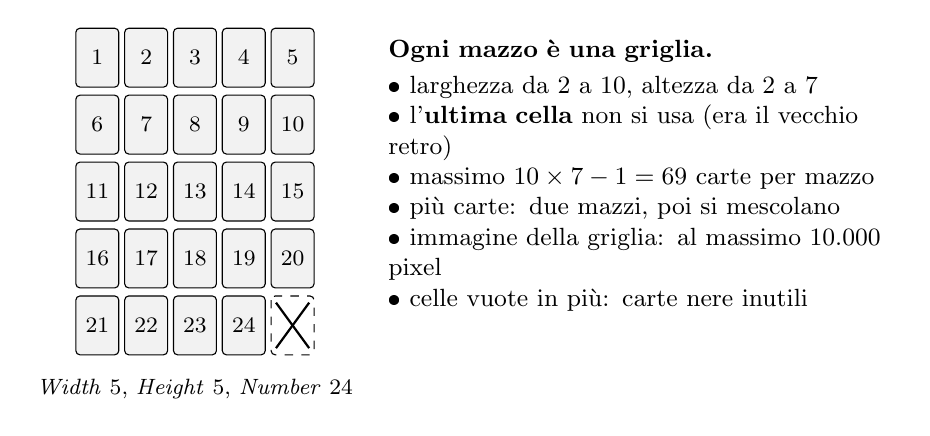
\begin{tikzpicture}[font=\footnotesize, x=0.62cm, y=0.85cm]
  % griglia 5x5
  \foreach \r in {0,...,4} {
    \foreach \c in {0,...,4} {
      \pgfmathtruncatemacro{\n}{\r*5+\c+1}
      \ifnum\n<25
        \draw[fill=gray!10, rounded corners=1.5pt] (\c,-\r) rectangle ++(0.88,-0.88);
        \node at (\c+0.44,-\r-0.44) {\n};
      \else
        \draw[dashed, fill=white, rounded corners=1.5pt] (\c,-\r)
          rectangle ++(0.88,-0.88);
        \draw[thick] (\c+0.1,-\r-0.1) -- (\c+0.78,-\r-0.78);
        \draw[thick] (\c+0.78,-\r-0.1) -- (\c+0.1,-\r-0.78);
      \fi
    }
  }
  \node[anchor=north, align=center] at (2.44,-5.1) {\emph{Width} 5, \emph{Height} 5,
    \emph{Number} 24};
  % nota a destra
  \node[anchor=west, text width=6.4cm, align=left, font=\small] at (6.2,-2.2) {
    \textbf{Ogni mazzo è una griglia.}\\[2pt]
    \textbullet\ larghezza da 2 a 10, altezza da 2 a 7\\
    \textbullet\ l'\textbf{ultima cella} non si usa (era il vecchio retro)\\
    \textbullet\ massimo $10\times7-1 = 69$ carte per mazzo\\
    \textbullet\ più carte: due mazzi, poi si mescolano\\
    \textbullet\ immagine della griglia: al massimo 10.000 pixel\\
    \textbullet\ celle vuote in più: carte nere inutili};
\end{tikzpicture}
\caption{La griglia di un mazzo custom nell'esempio di Ruggero: $5\times5$, con 24
carte e l'ultima cella inutilizzabile. Ricostruzione schematica.}
\label{a8:fig:griglia}
\end{figure}

\paragraph{I template dei mazzi.} Nella stessa cartella dei template dei dadi ci sono i
\textbf{Deck Templates}, con esempi di griglie (anche qui l'ultima carta non è usata).
Servono a poco: danno carte rettangolari e carte quadrate, ma ``che dimensione sono
queste carte? Io magari ho carte di dimensione diversa, strette e alte. Come
faccio?''. La griglia si può comporre a mano con qualunque programma, anche Photoshop,
mettendo le carte ``a manina una di fianco all'altra'', ``ma impazzite senza se e senza
ma''.

\subsection{Il Deck Editor}
\label{a8:sec:deck-editor}

Per questo, nella cartella \emph{Modding}, alla voce \emph{Deck Builder}, Tabletop
Simulator ha un \textbf{software secondario}: il \textbf{TTS Deck Editor}. Prima
pessima notizia: \textbf{non esiste per Mac}. ``Spero che abbiate dei compagni di gruppo
con Windows''. (E Ruggero ricorda che fare un gioco da tavolo non è obbligatorio:
``potete fare anche giochi pervasivi, LARP, giochi di ruolo''.)

Il Deck Editor ``è questa orripilezza qua, sembra fatto da un ingegnere''. La
procedura che Ruggero mostra (figura~\ref{a8:fig:mazzo}):
\begin{enumerate}
  \item \textbf{Nuovo mazzo}: il programma chiede larghezza e altezza della griglia,
        ``esattamente quelli che TTS ci chiede''. Ruggero sceglie $5\times5$. La
        griglia è ``grigia su grigia'', quindi non si vede (``un altro aspetto della
        brillantezza geniale dei programmatori''): compare solo quando ci si
        trascinano dentro le carte.
  \item Si \textbf{trascinano} le immagini delle carte nella griglia e le si copia
        quante volte serve. Nell'esempio: quattro copie dei numeri dal 2 al 6 e
        quattro Jack, ``a caso, non è un mazzo reale''.
  \item \textbf{File, Save Deck As}: si salva nella propria cartella di lavoro un file
        \texttt{.tsdb} (Ruggero lo chiama ``mazzo''). Ma Tabletop Simulator
        \textbf{non apre i \texttt{.tsdb}}: quel file serve solo a riaprire il mazzo nel
        Deck Editor.
  \item \textbf{File, Export}, con due accorgimenti: \textbf{togliere la spunta da
        Upload Image} (le immagini si caricano a mano, non online) e impostare
        \textbf{Max Deck Size a 10.000}. È ``una \emph{safety measure}'': se le carte
        sono gigantesche, il programma le ridimensiona in modo che la griglia non
        superi i 10.000 pixel, perché ``Tabletop Simulator crasha con le immagini più
        grosse di 10.000 pixel''. Si esporta e si ottiene \textbf{l'immagine della
        griglia}.
  \item In Tabletop Simulator, nel Custom Deck: l'immagine della griglia come fronte
        (in cloud), un retro generico (``questo blu mi va bene''), griglia $5\times5$,
        numero 24.
  \item \textbf{Sideways}: è un'opzione vestigiale, ``non spuntatela''; serviva ai
        vecchi mazzi, che non potevano avere carte orizzontali.
  \item \textbf{Backs is hidden}: \textbf{va spuntata}.
  \item \textbf{Import}, ``ed eccolo qua: abbiamo il nostro mazzo''.
\end{enumerate}

\paragraph{Backs is hidden e le mani.} Ruggero mostra a che cosa serve l'ultima spunta.
Dà delle carte alla propria mano e ad altre mani: le carte esistono, ma lui non vede
che cosa c'è nelle mani altrui. Cambiando colore e passando al giallo, vede il giallo e
non vede più l'arancione. \emph{Backs is hidden} significa questo: quando una persona
ha una carta in mano, quella carta è nascosta, e nelle mani degli altri si vede
\textbf{il retro} delle carte anziché il fronte.

\begin{figure}[htbp]
\centering
\begin{tikzpicture}[
    font=\small,
    passo/.style={draw, thick, rounded corners, text width=3.3cm, align=center,
      minimum height=1.25cm, fill=gray!10},
    file/.style={draw, dashed, rounded corners, text width=2.5cm, align=center,
      minimum height=0.8cm, font=\footnotesize},
    freccia/.style={-{Stealth[length=2.5mm]}, thick}
  ]
  \node[passo] (a) at (0,0) {\textbf{Deck Editor}\\ nuovo mazzo, griglia $W\times H$};
  \node[passo] (b) at (4.2,0) {trascinare e copiare le \textbf{carte}};
  \node[passo] (c) at (8.4,0) {\textbf{Export}: niente Upload Image, Max Deck Size
    10.000};
  \node[passo] (d) at (8.4,-2.4) {\textbf{TTS}, Custom Deck: fronte (cloud), retro,
    $W$, $H$, numero};
  \node[passo] (e) at (4.2,-2.4) {Sideways \textbf{no}, Backs is hidden
    \textbf{sì}, Unique Backs se serve};
  \node[passo] (f) at (0,-2.4) {\textbf{Import}: il mazzo è sul tavolo};
  \node[file] (s) at (4.2,1.6) {\texttt{.tsdb}: si riapre solo nel Deck Editor};
  \draw[freccia] (a) -- (b);
  \draw[freccia] (b) -- (c);
  \draw[freccia] (c) -- (d);
  \draw[freccia] (d) -- (e);
  \draw[freccia] (e) -- (f);
  \draw[freccia, dashed] (b) -- node[right, font=\footnotesize] {Save Deck As} (s);
\end{tikzpicture}
\caption{Il flusso di lavoro per creare un mazzo custom, come lo mostra Ruggero. Il
file \texttt{.tsdb} conserva il mazzo per le modifiche successive; a Tabletop
Simulator serve l'immagine esportata.}
\label{a8:fig:mazzo}
\end{figure}

\subsection{Le domande di Gianmarco}
\label{a8:sec:mazzo-domande}

\paragraph{Gli angoli arrotondati.} Gianmarco si è perso una cosa: l'arrotondamento
degli angoli delle carte l'ha fatto Ruggero nelle immagini? Sì e no. Ruggero ha
scaricato da internet un kit di carte singole, ``ce ne sono mille online'', già con gli
angoli arrotondati; ma nelle opzioni custom le carte sono impostate come arrotondate.
Impostandole rettangolari senza arrotondamento, gli angoli diventano neri, perché il
software riempie con il nero la trasparenza dell'immagine. Quando invece le si imposta
arrotondate, è il software ad arrotondarle ``a manina'', e infatti l'arrotondamento
del mazzo è un po' meno accentuato di quello delle immagini.

\paragraph{Più celle che carte.} ``È una domanda veramente stupida'': che cosa succede
se si mette una griglia $6\times6$ e poi un numero diverso dalle carte reali? Ruggero
lo mostra sul $5\times5$, impostando 35 carte: ``ti dà carte nere che non servono''.

\subsection{Carte con retri diversi}
\label{a8:sec:retri}

Finora le carte avevano tutte lo stesso retro. Per un mazzo in cui \textbf{ogni carta
ha il suo retro}: Ruggero copia il file \texttt{.tsdb} (``lo chiamo mazzo retro, così
lavoriamo su un mazzo diverso'') e vi compone la versione ``dark'' delle stesse carte,
nelle stesse posizioni (i numeri dal 2 al 6 neri, e il Jack). Nel Custom Deck, come
fronte resta la griglia di prima; come retro si carica la \textbf{seconda griglia, che
dev'essere identica} nella disposizione; si spunta \textbf{Unique Backs}. Importato, il
mazzo ha ``ognuna il suo retro''. È anche la risposta alla domanda di uno studente sulle
carte a doppia faccia, come quelle di \emph{Taboo}\footnote{``Tabu'' nella
trascrizione.}.

\subsection{La carta singola e le carte bucate}
\label{a8:sec:bucate}

\paragraph{La carta singola.} Il \textbf{Custom Card} chiede semplicemente fronte e
retro, ``senza tutto il resto''. Ruggero crea una carta con il re bianco davanti e il re
nero dietro: una carta singola, che si può mettere insieme alle altre.

\paragraph{Si possono bucare le carte?} Una studentessa chiede se le carte possono essere
forate, ``tipo una sorta di stencil''\footnote{La trascrizione dice ``una sorta di
stendarda'' e poi ``una sorta di scherzo''; dal seguito si capisce che si parla di
carte con dei fori, attraverso cui si vede ciò che sta sotto.}. Sì, perché Tabletop
Simulator gestisce la trasparenza. Ruggero copia il re, lo apre in Photoshop (``per
bucare le cose sono più comodo'') e ci fa un buco e un taglio scanalato di fianco;
basta un qualunque PNG con della trasparenza. Ricaricata, la carta \textbf{è bucata}:
si vede attraverso. ``Attenzione, però'': è bucata \textbf{l'immagine}, ma non è
bucata la \textbf{collisione}; un oggetto appoggiato sopra il buco non ci passa. E
il retro può anche non essere bucato: Ruggero ha bucato solo uno dei due lati, ``una
carta che non può esistere fisicamente''. La carta ha comunque uno spazio fisico che
non si può cambiare. Se si vogliono carte con uno \textbf{spazio fisico bucato}, si
usa il \textbf{token}, che gestisce la trasparenza \emph{anche} nella collisione: un
token ingrandito, appoggiato su un altro oggetto, non collide dove è trasparente.

% ---------------------------------------------------------------------
\section{Il tabellone senza cornice}
\label{a8:sec:tabellone}

Resta il problema della plancia con la cornice di legno
(sezione~\ref{a8:sec:plance}). ``Già lo sapete a questo punto come si fanno i
tabelloni'': \textbf{non li si importa come plance, li si importa come token}. Si crea
un token con una \textbf{profondità molto bassa}, gli si dà l'immagine del tabellone,
lo si ingrandisce in formato tabellone e lo si \textbf{blocca} sul tavolo. ``Anche se
tecnicamente, per TTS, è un token, questa per noi è una plancia''.

\paragraph{La prima pausa.} ``Ora vi darei forse dei minuti di pausa prima di passare
alla prossima fase, se vi va''. ``Se non è già troppo tardi, forse vi ho già consumato
troppo''. Pausa di sette minuti: si riprende alle \textbf{18:40}.

% ---------------------------------------------------------------------
\section{Penna, testo e fogli di carta}
\label{a8:sec:penna}

Al rientro Tiziana saluta (``nessun problema, Tiziana, va benissimo'') e, a quanto
si capisce, lascia la lezione. Ruggero riapre alle domande su quanto visto finora:
caricare componenti, aggiungerli al tavolo.

\paragraph{Esistono delle penne?} Una studentessa chiede se esistono delle penne, per i
giochi in cui bisogna appuntare dei punti o scrivere delle cose. Sì: c'è lo strumento
\textbf{Draw}, la penna, in alto a sinistra, di cui si può cambiare il colore e con cui
si disegna e si scrive sui componenti. (Ruggero si accorge di non aver ancora
ricondiviso lo schermo dopo la pausa: ``giustamente, se no non vedete''.) Ma la penna
non è un componente che si aggiunge: è uno degli \textbf{strumenti base} di TTS, come
il \emph{Grab} e lo strumento \textbf{Testo}. Sono strumenti usati solo nei giochi che
li richiedono, per esempio i \emph{party game} in cui si disegna.

\paragraph{Il foglio di carta.} Quello che manca è il foglio. Ma il foglio può essere
un \textbf{tile} o un \textbf{token bianco} su cui si disegna con la penna nera; oppure
si può usare una texture di carta. O, ancora, si apre un \textbf{tavolo custom} con una
texture bianca: allora ``tutto il tavolo è il nostro tabellone''.

% ---------------------------------------------------------------------
\section{Salvare e pubblicare il modulo}
\label{a8:sec:workshop}

Il modulo ha luce, tavolo, sfondo e componenti. Come lo si salva?

\paragraph{Save \& Load: solo in locale.} La prima opzione è nel menu \textbf{Games},
alla voce \textbf{Save \& Load}. Ruggero salva il modulo come ``Prototipo''; il
salvataggio compare nell'elenco e, cliccandoci, ricarica il modulo così com'era, anche
dopo aver cambiato stanza: ``si ricorda tutto quello che c'era''. Ma un salvataggio è
\textbf{usabile solo in locale}: non lo si può mandare a un \emph{publisher} perché lo
valuti. Per questo bisogna caricarlo come modulo sul \textbf{Workshop} di Steam, ``e
fare questa cosa è un po' più complesso''.

\subsection{Upload e Update}
\label{a8:sec:upload}

Dal menu \textbf{Modding}, la voce \textbf{Workshop Upload} apre una finestra con due
schede:
\begin{description}
  \item[Upload Workshop] si usa \textbf{solo la prima volta} che si carica il
        modulo;
  \item[Update Workshop] si usa per \textbf{tutti gli aggiornamenti} successivi, ``ed
        è più semplice''.
\end{description}

\paragraph{Le informazioni del modulo.} Prima di caricare conviene compilare le
\textbf{Info} del modulo (dal menu del gioco): nome, tipologia, complessità, tempo di
gioco, numero di giocatori, \emph{tag} del Workshop. ``Queste sono informazioni
meccaniche del Workshop''. Ruggero imposta: tipo \emph{game}, complessità bassa,
30--60 minuti, da 2 a 4 giocatori, nome ``prototipo brutto''. (Nel farlo, si accorge di
aver aggiunto per sbaglio un modulo: ``è un inferno, adesso''.)

\paragraph{Il caricamento.} Nell'Upload si scrivono il \textbf{titolo} (``prototipo
brutto''), una \textbf{descrizione} (``quello che volete, lasciamola uguale al
titolo'') e un'\textbf{immagine di anteprima}: ``mi sembra \emph{fitting} metterci la
texture del legno''. Si fa Upload; dopo qualche secondo compare in alto una scritta
verde: il modulo è caricato. Un \emph{pop-up} mostra un numero, l'identificativo del
Workshop, e raccomanda di conservarlo. ``Non ce ne frega niente'': si recupera quando
si vuole, ``non dobbiamo salvarlo o esplodere il mondo''.

\paragraph{La pagina del Workshop.} Nella libreria di Steam, su Tabletop Simulator, c'è
la voce \textbf{Workshop}; da lì, \textbf{i tuoi oggetti}, \textbf{oggetti
pubblicati}. C'è ``prototipo brutto'', con la sua pagina, ``esattamente come le
altre, solo che più brutta'', con il tasto \textbf{Iscriviti} come gli altri moduli.
In alto, però, c'è scritto che la visibilità attuale è \textbf{nascosta}: solo l'autore
può vederlo.

\subsection{La visibilità: unlisted}
\label{a8:sec:visibilita}

Dalla pagina si cambia la visibilità: \textbf{pubblico}, \textbf{solo amici},
\textbf{non in elenco} (\emph{unlisted}), \textbf{nascosto}. Le opzioni che servono sono
due; ``le altre sono delle mezze vie che non servono a nessuno''.
\begin{description}
  \item[Pubblico:] chiunque può entrare nel modulo, guardarlo, copiare le cose,
        prendere i componenti, salvarsi oggetti e immagini.
  \item[Unlisted:] lo vede solo chi riceve il \textbf{link diretto}. L'URL del modulo
        è in alto nella pagina; oppure, tasto destro sullo sfondo, \emph{Copia URL
        della pagina}.
\end{description}
\textbf{Per questo corso, i moduli si pubblicano unlisted}, ``se dovete farlo''. La
pagina del Workshop si può modificare come quelle degli altri giochi (Ruggero ne apre
una come esempio): descrizione, titolo, altre immagini, screenshot, ``paro paro''.

\begin{figure}[htbp]
\centering
\begin{tikzpicture}[
    font=\small,
    passo/.style={draw, thick, rounded corners, text width=2.7cm, align=center,
      minimum height=1.3cm, fill=gray!10},
    locale/.style={draw, dashed, rounded corners, text width=2.7cm, align=center,
      minimum height=1.3cm},
    freccia/.style={-{Stealth[length=2.5mm]}, thick}
  ]
  \node[locale] (s) at (0,1.8) {\textbf{Save \& Load}\\ \footnotesize solo sul proprio
    computer};
  \node[passo] (i) at (0,0) {\textbf{Info}: nome, tipo, complessità, tempo,
    giocatori};
  \node[passo] (u) at (3.5,0) {\textbf{Workshop Upload}: titolo, descrizione,
    anteprima};
  \node[passo] (p) at (7.0,0) {Steam: \textbf{pagina} del modulo (nascosto)};
  \node[passo] (v) at (10.5,0) {visibilità \textbf{unlisted}: si condivide il
    link};
  \node[locale] (up) at (3.5,-2.0) {\textbf{Workshop Update}\\ \footnotesize per ogni
    modifica successiva};
  \draw[freccia] (i) -- (u);
  \draw[freccia] (u) -- (p);
  \draw[freccia] (p) -- (v);
  \draw[freccia, dashed] (up) -- (u);
\end{tikzpicture}
\caption{Dal salvataggio locale al modulo condivisibile, secondo la procedura di
Ruggero. La prima pubblicazione si fa con l'Upload, tutte le successive con l'Update.}
\label{a8:fig:workshop}
\end{figure}

% ---------------------------------------------------------------------
\section{Prendere i componenti degli altri}
\label{a8:sec:riuso}

\paragraph{Save Object.} Una studentessa chiede: quindi chiunque potrebbe prendere i
componenti di altri giochi, se li si fa pubblici? ``Ah, sì, certo. Anzi, adesso arrivo
a parlarvi di questo''. Se serve un componente particolare trovato in un altro modulo,
lo si può salvare. Ruggero apre un modulo pubblico\footnote{``Farm Race'' nella
trascrizione: il titolo del modulo non è verificabile.} che ha dei token a forma di
animale e prende una \textbf{gallina}: tasto destro, \textbf{Save Object}, e la si
chiama ``gallina''. Tornati nel proprio modulo, dal menu Oggetti c'è l'ultima voce che
non aveva ancora nominato, \textbf{Oggetti salvati}: la gallina è lì. ``Così come io
ho salvato un granchio col coltello, per esempio. Può sempre essere utile''. ``Ho anche
un granchio senza coltello''.

\paragraph{Dove finiscono gli oggetti salvati.} Una studentessa ha salvato un mazzo di
carte, con immagini caricate da lei, ma non lo trova più. Se ha fatto un \emph{Save
Object}, dovrebbe trovarlo negli oggetti salvati; caricare le immagini da qualche parte,
da sola, non salva l'oggetto. In ogni caso, \textbf{tutto quello che si è caricato} è
nel menu \textbf{Modding}, alla voce \textbf{Cloud Manager}. È anche buona pratica
farci un po' di pulizia.

\subsection{Quando la sorgente sparisce}
\label{a8:sec:sorgente}

Gli oggetti salvati restano utilizzabili \textbf{finché chi ha caricato l'immagine la
tiene online}. Ruggero ha appena cancellato dal cloud un'immagine (una carta,
``lanciata nel sole'') e vuole mostrare che cosa succede: ricaricando il modulo
dovrebbero comparire degli errori. Ma sul suo computer non succede, perché le immagini
sono ancora nella \emph{cache}, e per svuotarla dovrebbe chiudere e riaprire il software
(``non ho voglia''). Allora condivide il link del Workshop perché qualcuno lo provi.

\paragraph{Discord, non la chat.} Prova a scrivere il link nella chat della lezione;
``No, su Discord, Ruggero, altrimenti non possiamo copiarlo e incollarlo''. Ha ragione:
gli anni scorsi non era così, ma la piattaforma ha cambiato le impostazioni di
sicurezza (``con la questione delle IA hanno aumentato le difese, ma verso cosa?
Comunque, questi sono i miei rant''). Uno studente vorrebbe provare a condividere lo
schermo, ma è collegato dal computer aziendale, che non gli permette di installare
Steam. Ruggero allora descrive l'effetto: chi carica un modulo a cui manca la sorgente
di un'immagine vede un \textbf{messaggio di errore rosso} in alto, ripetuto nella chat
del gioco, e il componente può non caricarsi affatto.

\paragraph{La gallina era un modello 3D.} Il caso della gallina è istruttivo. Aprendo
il suo menu custom, si scopre che non è un token: è un \textbf{modello 3D custom}, a cui
qualcuno ha dato una \textbf{mesh}, un'immagine \textbf{diffuse} e un \textbf{collider}.
Per non perderla, bisognerebbe salvare sul proprio computer queste tre cose
separatamente: ``roba da uscirci impazziti''. Quindi: \textbf{attenzione a che cosa si
salva}, e da dove viene.

\paragraph{I moduli di meeple.} Esistono però moduli che fanno ``il lavoro sporco'' per
gli altri. Ruggero ne usava uno ``che era una bomba atomica'', in cui qualcuno aveva
caricato più di cento modelli 3D di \emph{meeple} di forme diverse; lo riapre, il
software va in crash, e quando lo riapre davvero ne è sopravvissuta circa la metà:
``RIP''. Ma cercando ``meeples'' nel Workshop di Tabletop Simulator si trovano vari
moduli che hanno l'unico scopo di fornire segnalini di varie forme\footnote{La
trascrizione cita un modulo che rende con ``Wooden Talker'' e un altro, ``Mipolorama'',
probabilmente un gioco di parole su \emph{meeple}; i titoli esatti non sono
ricostruibili.}: un riccio, un omino col cappello, barche, camion, stivali, ``tutti
ricolorabili''. ``Avete l'imbarazzo della scelta''.

% ---------------------------------------------------------------------
\section{I moduli di Ruggero}
\label{a8:sec:moduli}

``Ora vi faccio vedere cosa si può fare su Tabletop Simulator quando si lavora per fare
dei moduli'': i moduli che Ruggero ha fatto in passato, ``dai più \emph{easy} ai più
complessi''.

\subsection{Un gioco di carte}
\label{a8:sec:mod-carte}

Il primo è un gioco ``molto \emph{card based}'' fatto per un lavoro\footnote{La
trascrizione dice ``quando lavoravo per Camon''; il nome del committente non è
ricostruibile.}. C'è il \textbf{regolamento} in alto, che si apre a doppia pagina;
\textbf{nove mazzi} di carte; un \textbf{tabellone} con i segnalini che segnano le
risorse e che \textbf{scattano in posizione} (``non stanno a metà via''); sacchetti con
i dadi; plance con i tracciati e i segnalini delle risorse. ``Liscio, regolare: tutte
cose che in teoria dovreste già saper fare anche voi''.

Ruggero ne approfitta per interrogare la classe:
\begin{itemize}
  \item La \textbf{bandiera}, che componente è? Un \textbf{token}, perché ha una forma
        non regolare; e infatti, girata, è specchiata dietro. Lo stesso vale per un
        segnalino col numero 5, specchiato sul retro.
  \item Questi segnalini rotondi? Sono \textbf{tile} rotondi: il retro non è
        specchiato.
  \item La \textbf{plancia}? È una tessera.
  \item Le carte sono mazzi custom. Un mazzo è di \textbf{18 carte}: che griglia ha
        usato? Uno studente propone $7\times3$, ``e poi ne butti via due''; un altro
        $10\times2$. È un $10\times2$. Con $7\times3$ si sprecherebbero tre celle
        (21 meno 18), e una comunque non si può usare; $9\times2$ non basta, perché
        l'ultima cella non è usabile; con 18 carte le celle sprecate sono almeno due.
        ``Potevo fare anche un $5\times4$''.
\end{itemize}

\subsection{La demo di un gioco grande}
\label{a8:sec:mod-cyberpunk}

Il secondo è il modulo completo della \textbf{demo} di un gioco da tavolo grande,
legato a \emph{Cyberpunk}\footnote{La trascrizione dice ``il modulo completo della demo
di Cyberpunk. Destiny 7''; più avanti Ruggero cita il suo lavoro su ``Marvel United e
Cyberpunk'' e una cartella ``Cyberpunk'' nel suo Cloud Manager. Il titolo esatto del
gioco non è ricostruibile dalla trascrizione.}, che ci mette un po' a caricare perché
``ha tonnellate di roba'': un tabellone gigantesco con segnalini ovunque, pile di token
di forma custom, miniature su miniature, carte di diversi mazzi. Il \emph{publisher}
voleva anche la \textbf{scatola}, ``perché volevano far vedere quanto bella è la
scatola''; il regolamento è sospeso in aria, ``perché la gente sta male. Richieste del
publisher, ma va bene''. Ci sono token, carte custom con fronte e retro separati: cose
più complesse per forme e quantità, ma che gli studenti sanno ormai fare. Le
\textbf{miniature} invece sono \emph{asset bundle}: quelle no.

\paragraph{Che cosa c'è di strano?} ``Chi la nota?''. Uno studente: non c'è il tavolo.
Esatto: Ruggero usa il \textbf{non-tavolo}, l'opzione \emph{None}. È il motivo
promesso all'inizio (sezione~\ref{a8:sec:tavoli}). Le mani dei giocatori si possono
spostare dove si vuole; e siccome il software è un simulatore fisico, il tavolo lo crea
lui: un \textbf{token gigantesco}, molto piatto e sottile, con una texture, reso
\textbf{non interagibile} e \textbf{bloccato}. La texture sfuma verso il nero, e con lo
sfondo monocromatico nero il bordo del tavolo si confonde con lo sfondo e non si nota.
In streaming si vede poco; cambiando lo sfondo, si vede subito.

\subsection{Gli ancoraggi}
\label{a8:sec:ancoraggi}

Una cosa che Ruggero non ha spiegato, ``perché non vi servirà per questo prototipo'',
sono gli \textbf{snap point}, i \textbf{punti di ancoraggio}. In certe celle, un
segnalino o una carta appoggiati si posizionano da soli nel punto giusto: ``questo
token, quando va avanti, si ferma lì''. Attivando lo strumento degli ancoraggi (un
puntino verde in fondo al menu), si vede che tutti i tracciati del modulo e delle plance
sono ancorati.

\paragraph{Come si fanno.} ``A mano'', spiega Ruggero: si copia l'oggetto più volte, lo
si allinea con lo strumento \textbf{Gizmo}, che dà una precisione maggiore, e quando
una copia è nel punto giusto ci si clicca sopra con lo strumento degli ancoraggi, che
crea un ancoraggio lì: ``questo componente scatterà esattamente qua''. Poi si cancellano
le copie in più, e gli ancoraggi restano. ``Uno sbatti infinito. Però si può fare''.
Gli ancoraggi valgono per un solo tipo di componente? No: li si può dedicare a vari
componenti, anche con dei \textbf{tag}. Ruggero mostra un gioco ``devastante'', in cui
ogni casellina è un ancoraggio per delle piccole buste, e le teste di certi pezzi vanno
ad agganciarsi al loro posto.

\paragraph{Che cosa si chiede al corso.} ``Noi non vi chiediamo questo livello di
pulizia del prototipo''. Ruggero mostra allora un prototipo su cui sta lavorando in
quel periodo: è ancora grezzo, le icone e le grafiche non sono definitive, alcune carte
non hanno ancora l'illustrazione (``dovrebbe avere una grafica, ok? È un prototipo'').
``Non è neanche questo quello che ci aspettiamo da voi''.

\subsection{Un gioco di ruolo con lo scripting}
\label{a8:sec:mod-gdr}

Tabletop Simulator non è solo per i \emph{board game}: si possono fare anche giochi di
ruolo. Ruggero mostra un modulo fatto per un gioco di ruolo\footnote{La trascrizione
lo chiama ``Magic of the Inventory''; il titolo non è verificabile.}, in cui si è dovuto
usare lo \textbf{scripting}: per esempio, bisognava poter scrivere la descrizione degli
oggetti, quindi le carte sono \textbf{scrivibili}, e certi componenti permettono di
cambiare i numeri.

\paragraph{Non è obbligatorio.} Tornando al ``prototipo brutto'', Ruggero ripete che
Tabletop Simulator probabilmente non servirà a tutti i gruppi: servirà a chi fa giochi
da tavolo, magari un po' ibridi. \textbf{Non è obbligatorio} per il corso; ma per chi è
interessato ai \emph{board game}, è il software usato nel settore.

% ---------------------------------------------------------------------
\section{Perché proprio Tabletop Simulator}
\label{a8:sec:alternative}

Una domanda ``molto laterale'': quanto è legato il settore a Tabletop Simulator? Se
uscisse un simulatore molto migliore, lo si adotterebbe? Ne sono già usciti altri,
risponde Ruggero, per esempio \textbf{Tabletopia}, ma ``sono tutti peggiori in termini
di usabilità''. Tabletopia è gratuito, ``ma fa schifo'', e infatti lo usano in
pochissimi, perché non ha la metà delle funzioni di Tabletop Simulator\footnote{La
trascrizione dice ``non ha la metà delle funzioni che Tabletopia ha'': dal contesto è
evidente che il confronto è con Tabletop Simulator.}.

\paragraph{Le funzioni che non ha mostrato.} E Ruggero, ``per semplicità e per non
farvi impazzire'', ha taciuto cose molto più tecniche:
\begin{itemize}
  \item si possono \textbf{creare nuove mani}, o ridimensionarle: una mano rossa
        molto più grande (``di boh, 30''), per un gioco in cui si tengono in mano
        tantissime carte;
  \item si possono \textbf{incollare} i componenti tra loro con lo strumento della
        \textbf{catenella} (i \emph{joint}): un dado ingrandito incollato sopra un
        cubetto diventa un oggetto solo;
  \item si possono fare \textbf{plance con alloggiamenti}, ancorati, in cui inserire
        altri componenti: Ruggero ne mostra un vecchio prototipo (``è brutto,
        ignoratelo'');
  \item si possono giocare anche i \textbf{legacy}, grazie allo strumento degli
        \textbf{adesivi}: Ruggero crea un adesivo con la sua ``A'' e lo attacca a una
        carta (prima, per sbaglio, sul mazzo intero: ``sono scemo''); la carta,
        mescolata con le altre, conserva l'adesivo.
\end{itemize}
``È che abbiamo una quantità di strumenti qua dentro che è delirante. Non ve ne ho fatti
vedere neanche la metà, vi giuro'': l'angolo di rotazione, l'altezza a cui si
sollevano gli oggetti, ``tutte cose tecniche che non vi servono adesso, ma in cui, se
imparate questo software, c'è un \emph{rabbit hole}''. Non è possibile comprimerlo in
tre ore. L'obiettivo di oggi è dare ``il minimo necessario per riuscire a fare un gioco
che abbia dei componenti, dei dadi, delle carte, un tabellone, una plancia''; per le
idee strambe, si scrive a Ruggero.

\paragraph{Cancellare il modulo.} Ultima procedura: come si cancella un modulo? ``Il
prototipo è troppo brutto per tenerlo''. Dalla pagina del Workshop, in fondo,
\textbf{Elimina}: il modulo viene cancellato dal Workshop, ma non del tutto, perché
resta il \textbf{salvataggio} locale. Cancellato anche quello, ``se ne va via tutto''.

% ---------------------------------------------------------------------
\section{Prototipi in scala}
\label{a8:sec:scala}

Ruggero apre alle domande: ``questa ultima parte della lezione è per rispondere a voi''.
Uno studente, ``per curiosità'': quanto sono verosimili i prototipi che Ruggero
prepara per i \emph{publisher}? Lo scopo è arrivare a una prova realistica?

\paragraph{Estremamente accurati.} ``Quelli che faccio io sono estremamente
accurati'': i componenti sono davvero \textbf{in scala}. Quelle carte sono in formato
poker, 88 mm; quelle altre nel formato delle carte di \emph{Dixit}\footnote{``Le carte
formato di exit'' nella trascrizione: con ogni probabilità \emph{Dixit}, le cui carte
grandi sono un formato standard del settore.}; le miniature hanno la base delle
dimensioni delle miniature reali. Il motivo è il \emph{playtest}: i componenti devono
essere ``il più simulati possibile'' per avere un playtest vicino a quello reale,
perché il playtest verifica anche \textbf{gli spazi}. ``Mettiamo che io ho un distretto,
e devo sapere se ci stanno otto miniature in questo distretto. Come faccio a saperlo,
se io non le muovo?''. Un playtest deve poter dire: ``un po' strettine, ma ci stanno''.
E se gli spazi del tabellone devono contenere le carte, le carte devono essere in scala
con il tabellone, e così i token e le miniature: ``per forza di cose si va a creare
tutto in dimensioni reali''.

\paragraph{Si parte dal tabellone.} Anche prima, nei primi prototipi, il passaggio non
è diverso. Ruggero parte di solito \textbf{dal tabellone}, perché è la cosa più grande
e quindi la più facile da mettere in scala. Tabletop Simulator misura in griglia, in
pollici o in centimetri, \textbf{non in millimetri}: si lavora con i decimali dei
centimetri, e su una carta che misura ``8 virgola qualcosa'' è difficile capire se sia
88, 89, 85 o 86 mm. Su un tabellone di 350 mm l'errore pesa molto meno. Quindi: prima
il tabellone, poi tutto il resto in scala rispetto al tabellone.

\paragraph{Approfondimento: la fedeltà del prototipo.} La risposta di Ruggero mostra
che ``prototipo grezzo'' e ``prototipo in scala'' non sono in contraddizione. Il
prototipo che ha mostrato poco prima ha grafiche provvisorie e carte senza
illustrazione, ma le misure sono già quelle vere: la fedeltà \emph{grafica} è bassa,
quella \emph{spaziale} è alta, perché è lo spazio che il playtest deve verificare.
È lo stesso principio per cui Schell raccomanda di decidere, prima di costruire un
prototipo, quali domande deve aiutare a risolvere: quello che non serve a rispondere
può restare grezzo.

% ---------------------------------------------------------------------
\section{Aggiornare un mazzo e tenere in ordine il cloud}
\label{a8:sec:aggiornare}

\paragraph{Correggere una carta.} L'ultima domanda dello stesso studente è ``più
tecnica'': nei prototipi capita di dover correggere una carta. ``Ottima domanda, ottima
domanda''. Ruggero riprende il mazzo fatto prima e finge un errore di bilanciamento:
invece di due Jack servono, ``che so, due Jack e due regine''. Aggiorna il mazzo nel
Deck Editor, lo salva, lo \textbf{riesporta}, e nel menu custom del mazzo ricarica
\textbf{solo il fronte}, perché il retro non cambia. Con \emph{Search} si vedono le due
regine.

\paragraph{Correggere una sola immagine.} Poi un caso più fine. Ruggero modifica in Paint
una sola carta (la regina di quadri), salvando il file con lo stesso nome. Riaprendo il
\texttt{.tsdb}, il Deck Editor riprende le carte dalla cartella e mostra già la carta
aggiornata. Quindi: \textbf{se si mantengono uguali i nomi dei file}, si aggiorna la
singola immagine, si riesporta nella stessa cartella da cui il \texttt{.tsdb} prende le
carte, e il mazzo è aggiornato senza ricomporlo. ``Anche perché questi moduli si
aggiornano tante volte'': il modulo del gioco che Ruggero sta per pubblicare\footnote{La
trascrizione lo chiama ``Astronega'' e poi ``Astronica''; il titolo non è
ricostruibile con certezza.} è stato aggiornato \textbf{79 volte}. È quello con la
carta senza illustrazione: ``appena l'illustratore me la finisce, io riaggiorno
semplicemente quel file lì, e siamo a posto''.

\paragraph{Le cartelle nel Cloud Manager.} Una buona pratica: caricare le immagini in
cloud \textbf{dentro delle cartelle}. Nel suo Cloud Manager Ruggero ha una cartella per
ogni progetto: tutti i componenti del gioco di \emph{Cyberpunk} in una, quelli
dell'altro gioco in un'altra. ``Dividervi in cartelle vi serve anche per sanità
mentale'', altrimenti ci si ritrova con ``una sfilza di tutte le immagini che avete
usato, caricate a caso''.

\paragraph{Il limite dei 9.999 file.} Ed è buona pratica \textbf{cancellare} ciò che
non si userà. Non è un problema di oggi, ma Tabletop Simulator ha un \textbf{limite
fisso di 9.999 file} caricati. ``Sembrano tanti, e sono tanti se fate pochi giochi. Ma
vi giuro che il limite lo si raggiunge. Io l'ho già raggiunto più volte''. E i file si
cancellano \textbf{uno alla volta}, a mano: non c'è un'opzione per cancellarne di più.
``Lo so: sono pazzi''.

% ---------------------------------------------------------------------
\section{Un software di settore suo malgrado}
\label{a8:sec:storia}

\paragraph{Lo stupore di Rita.} Rita è colpita: per un software di questa portata, è
incredibile che manchino cose così elementari. Lei è abituata ai software Adobe, ``a un
altro tipo di possibilità''; ``però è molto interessante. La lezione di oggi mi ha
stimolato un sacco. Credo che starò tutta la notte a provare''. ``È un software
incredibile, Rita'', risponde Ruggero, ma ``fatto da tre appassionati che non hanno
ragionato per diventare un software di settore. Sono diventati un software di settore
contro la loro volontà''.

\paragraph{Le cose stanno cambiando.} Oggi ne guadagnano, e qualcosa si muove: dalla
pagina della comunità su Steam, nelle notizie, Ruggero mostra la \textbf{roadmap} che gli
sviluppatori hanno deciso di pubblicare dall'inizio dell'anno, ``finalmente, dopo dieci
anni e passa di software''. Stanno aggiornando il motore, ``dopo anni che glielo si
chiedeva''. E gli studenti hanno già visto una versione migliorata. Il Custom PDF,
quando Ruggero ha cominciato, \textbf{non esisteva}: si metteva sul tavolo il
\textbf{tablet} e ci si apriva un link al PDF. E se i file erano esportati in
\textbf{CMYK} anziché in \textbf{RGB}, il software andava in crash ``secco''; ora si
limita a dire che non accetta quel tipo di file. ``Per farti capire quanto fuori di
testa era questa gente''.

\paragraph{Studiare i moduli degli altri.} Un consiglio: ora che si sa come sono fatti i
componenti, si può aprire un modulo qualunque e studiarlo. Con tasto destro,
\textbf{Custom}, su un componente, si vede \textbf{che cosa è}: ``questi bellissimi
tokenoni qua cosa sono? Sono dei modelli o sono dei token? Sono dei token, fantastico.
Questi posso rifarli anch'io, so come farli''. Su un modulo aperto come
esempio\footnote{``Sputacular'' nella trascrizione: il titolo non è ricostruibile.} si
vede che certi segnalini sagomati sono token, perché il retro è specchiato.

\paragraph{Il token fronte-retro.} Esiste però un modo per fare token di forma
particolare con il retro \emph{dritto}: \textbf{incollarne due} con la catenella. ``È un
bello sbatti'', e Ruggero non ricorda più in quale modulo l'aveva fatto. Uno studente
chiede di rispiegarlo, e Ruggero lo rifà da zero: si crea un token con una forma
particolare (un \emph{meeple} giallo) e un secondo token con la stessa forma e il retro
voluto (rosso); dal menu \textbf{Options} si attiva la \textbf{griglia}, che allinea i
pezzi con precisione, così che siano nella stessa identica posizione, uno sopra l'altro;
con la \textbf{catenella} li si aggancia; si toglie la griglia. Il risultato è un token
custom con due facce diverse e il retro non specchiato.

% ---------------------------------------------------------------------
\section{Niente script}
\label{a8:sec:script}

Si possono fare ``cose fuori di testa'': \textbf{perni mobili} (\emph{joint}) per
attaccare gli oggetti, e soprattutto \textbf{script} che automatizzino delle cose. Ed è
qui che Ruggero mette l'unico divieto tecnico della lezione: \textbf{in questo corso
gli script non si fanno}. Il motivo si capirà nella lezione sul playtest: ``gli script
vi rendono più complesso testare cose particolari, e quindi remano contro la vostra
procedura di playtest''. E siccome si vuole un playtest utile e strutturato bene,
``quando arriveranno i playtest vi sarà chiaro perché gli script sono un problema''.

\paragraph{Approfondimento: perché l'automazione disturba il playtest.} La lezione sul
playtest è ancora lontana, ma il senso del divieto si può già intuire dalla
sezione~\ref{a8:sec:simulatore}. In un prototipo analogico i giocatori eseguono le
regole a mano, e proprio eseguendole le capiscono, sbagliano, le contestano: sono i
dati che un playtest raccoglie. Uno script che sposta i segnalini o calcola i punteggi
toglie questi momenti dal tavolo e nasconde il carico di gestione che il gioco stampato
avrà davvero. In più, ogni modifica alle regole tra un playtest e l'altro richiederebbe
di riscrivere il codice: il prototipo diventerebbe più lento da cambiare proprio nella
fase in cui deve cambiare più spesso.

\paragraph{La seconda pausa.} ``Abbiamo ancora mezz'ora di domande''. Silenzio: ``Tutto
chiaro? Non è possibile, non posso essermi spiegato così bene''. Uno studente prevede
che la prima volta che darà un modulo a qualcuno ``gli esploderà il computer''.
Ruggero propone un'altra pausa, fino alle \textbf{19:35}: ``liberatevi un attimo il
cervello, mi rendo conto che oggi è stata molto intensa''. Al ritorno risponderà a
domande e curiosità ``anche generali, non solo sul software, a tutto tondo''. Gianmarco
dice che non gli vengono domande; ``ma le domande verranno tra una settimana, tra un
mese. È normale''. Ogni anno qualcuno gli scrive giorni o settimane dopo: si può fare
questa cosa? La risposta è ``sì'', perché Tabletop Simulator ``è magia nera, è un patto
col diavolo'': sì, ma magari bisogna impazzire tre giorni su un modello 3D; oppure sì,
ma bisogna programmare, ``e piuttosto ti tagli le mani''.

% ---------------------------------------------------------------------
\section{Dopo la pausa: scorciatoie, fisica e destrezza}
\label{a8:sec:fisica}

``Rieccoci qua. Allora, come va? Come state? Io, stanco, venerdì pomeriggio, dopo tre
ore di Tabletop''. Se agli studenti ``si spacca tutto in testa'', è normale: ``è
traumatico''. Quando Ruggero ha cominciato a usarlo, ``odiarlo'' era un eufemismo: non
c'era la metà delle funzioni di oggi ed era molto più complesso. Ma ha ``tante cose
molto funzionali''.

\paragraph{Ingrandire.} Alcune cose da tutorial, che non ha mostrato: con il tasto
\texttt{Alt} si \textbf{ingrandiscono a schermo} le carte e gli oggetti; con il tasto
\texttt{M} si attiva la \textbf{lente} (\emph{Magnify}). (Uno studente gli fa notare
che non sta condividendo lo schermo: ``giusto, hai ragione. In effetti sono pazzo''.)
Dal menu di \texttt{Esc} ci sono tutte le scorciatoie.

\paragraph{La fisica dei componenti.} Ruggero non è entrato nel dettaglio del
\textbf{peso} delle cose: si può cambiare la fisica dei componenti, la \textbf{massa},
l'\textbf{attrito} con l'aria, l'attrito angolare\footnote{``La tritangolare'' nella
trascrizione; si intende con ogni probabilità l'attrito (o la resistenza) angolare,
che regola quanto un oggetto continua a ruotare.}, e perfino la \textbf{gravità} del
modulo. Lo mostra tirando dei dadi con la gravità bassissima e poi altissima. Serve,
per esempio, a fare dei \emph{dexterity game}.

\paragraph{Il minigolf.} La gente usa il software ``per fare le cose più folli''.
C'era un modulo di \textbf{minigolf}: si prendono le palline, si usa lo strumento
\emph{flick}, ``e ok''. ``La gente sta male. In positivo, chiaramente, in questo caso''.
Su Tabletop Simulator si possono fare giochi da tavolo ``nel senso più tradizionale del
termine'', \emph{wargame}, giochi di miniature, giochi di destrezza: ``ha un potenziale
gigantesco'', che però, con la sua interfaccia ``un po' \emph{cranky}, un po' \emph{old
school}'' e i suoi aspetti vestigiali, spesso non arriva.

% ---------------------------------------------------------------------
\section{Un consiglio: giocate The Box}
\label{a8:sec:thebox}

``Uno dei consigli che do sempre, se volete imparare a usare bene questo software e
volete farlo giocando'': giocare \textbf{\emph{The Box}}. È un gioco che \textbf{esiste
solo su Tabletop Simulator}, che ``non può esistere nella realtà per mille motivi che
vedrete se lo giocherete''. Ruggero lo apre, lo linka su Discord, e lo consiglia ``a
prescindere dal corso''.

\paragraph{Perché giocarlo.} ``Come paradigma di game design, questo gioco vi dà una
mano''. È un gioco ``che sulla carta non dovrebbe funzionare'', con un game design che
Ruggero trova ``anche brutto'', ma con ``un'esperienza incredibile da giocare''. E
ragionare sul perché un gioco fatto male dia un'esperienza che può essere molto
positiva ``è molto utile, lato game design''.

\paragraph{Come giocarlo.} ``Non leggetevi niente''. Si organizza una serata (tiene
fino a otto persone, ``se non ricordo male''), si apre un tavolo su TTS e si legge il
regolamento lì: è ``una manciata di pagine'', scritto ``in font gigantesco'', ``non è
bello da vedere''. Il gioco è ``bizzarro, strano'': tre scatole, una delle quali ne
contiene altre \textbf{80}, e un'altra altre \textbf{121}, con nomi bizzarri come
``B126'' o ``diametro infinito''. E fa interagire con moltissimi dei componenti visti a
lezione: è l'opzione consigliata per ``prendere confidenza con la varietà più disparata
di componenti''. (``Adesso che ve l'ho nominato, devo organizzare per giocarlo con
qualcuno, perché è bellissimo''.)

\paragraph{Approfondimento: imparare da un gioco ``brutto''.} Il consiglio di Ruggero
riprende un'idea che attraversa tutto il corso: l'esperienza del giocatore non coincide
con la qualità ``sulla carta'' delle regole. Nel lessico dei framework visti nelle
lezioni precedenti, un insieme di meccaniche discutibile può comunque produrre
dinamiche e un'esperienza memorabili, e capire \emph{perché} succede è un esercizio di
analisi più istruttivo che studiare un gioco ben fatto. Schell lo formula come
un'abitudine del designer: guardare all'esperienza prima che alle regole, e chiedersi
quali elementi la producono davvero.

% ---------------------------------------------------------------------
\section{Saturi}
\label{a8:sec:saturi}

``Oltre a TTS, come state?''. Una studentessa è ``saturatissima'' di cose apprese: deve
``fare un attimo ordine fra i pensieri'' per capire che cosa provare per prima e che
cosa chiedere. ``Certamente''; e di nuovo, a Ruggero si può scrivere per mail o su
Telegram. Un'altra è ``satura di nozioni, non riesco più ad apprendere''. Rita
ringrazia: ``è la lezione più bella finora per me''.

Ruggero è contento: questa lezione, per molti, è ``una mattonata''. Le classi sono
molto diverse, e capitano studenti che non hanno mai avuto confidenza con software
tecnici, per cui questa lezione ``è un po' una mazzata''; ``sono contento, Rita, che ti
sia piaciuta, anche perché abbiamo davvero sorvolato la punta dell'iceberg di Tabletop
Simulator, questo ve lo assicuro''.

% ---------------------------------------------------------------------
\section{Il playtest e il calendario del corso}
\label{a8:sec:calendario}

Una studentessa (``sempre le mie domande\ldots''): quanto è rilevante usare Tabletop
Simulator nel \emph{playtest}, e quanto invece è importante farlo \textbf{fisico}? ``Ti
sorprenderà sapere'' che c'è una lezione sul playtest. ``Immaginavo'', risponde lei, ``ma
lo faccio apposta: tu mi anticipi ogni volta le cose''; e, come ha visto, nelle lezioni
successive le cose vengono riprese.

Ruggero controlla quando, e già che c'è ripassa il resto del calendario
(tabella~\ref{a8:tab:calendario}).

\begin{table}[htbp]
\centering
\small
\begin{tabular}{@{}p{3.0cm}p{9.6cm}@{}}
\toprule
\textbf{Quando} & \textbf{Che cosa} \\
\midrule
lunedì (5 ottobre) & lezione con Beatrice, la seconda sulle \textbf{esperienze
ludiche} \\
venerdì (9 ottobre) & lezione sul \textbf{paragame}\protect\footnotemark, ``una delle
mie preferite''; si parlerà anche di TTS, ``ma a tangente'' \\
12 ottobre & il \textbf{pitch}: niente lezione, il \emph{check} dei progetti \\
fino a novembre & periodo di lavoro senza lezioni \\
6 novembre & lezione con \textbf{Diego} sull'\textbf{RNG} (la casualità) \\
9 novembre & \textbf{playtest} con Ruggero: ``playtest e metodi etnografici di raccolta
feedback'' \\
dopo & \textbf{gioco di ruolo da tavolo} con Daniele \\
dopo & ``l'ondata lunga'' di \textbf{sviluppo 1} e \textbf{sviluppo 2} con
\textbf{Marta}: \emph{development}, modelli matematici, bilanciamento e altri aspetti
dello sviluppo \\
dopo & \textbf{produzione} con \textbf{Flavio} \\
dopo & altro periodo di lavoro \\
11 dicembre & \textbf{final review} \\
dopo la review & \textbf{tavola rotonda} con editori e persone del settore \\
\bottomrule
\end{tabular}
\caption{Il calendario del resto del corso come lo ripassa Ruggero. Le date tra
parentesi sono ricostruite dal contesto; le altre sono dette a voce.}
\label{a8:tab:calendario}
\end{table}
\footnotetext{La trascrizione dice ``quella sul paragame''; il termine non è spiegato
nella lezione.}

\paragraph{La tavola rotonda.} Dopo la \emph{final review}, nella lezione di
\textbf{tavola rotonda} i docenti portano \textbf{editori} e altre persone del settore
a dare un feedback sui progetti: un punto di vista che non sia solo quello degli
insegnanti, ma di chi lavora nel settore. Gli ospiti si scelgono \textbf{in base ai
giochi dei gruppi}. L'anno scorso, ``per varie cose'', non è uscito neanche un
\emph{board game}: giochi di ruolo, LARP, giochi pervasivi, ma nessun gioco da tavolo; e
quindi non sono stati chiamati editori di giochi da tavolo, perché ``non aveva senso
dare feedback da qualcuno che lavora nel board game a un gioco di ruolo''. Anche
quest'anno la tavola rotonda sarà calibrata su quello che i gruppi faranno. La
studentessa aggiunge che finora non ha mai strutturato i prototipi su TTS, li ha sempre
fatti fisici; ``non è un problema''.

% ---------------------------------------------------------------------
\section{Domande e risposte, alla rovescia}
\label{a8:sec:rovescia}

``Avete altre domande, dubbi? Avete risposte? Mi date le risposte, io vi credo''. Uno
studente sta al gioco: ``È blu, è blu, è blu''. E poi: ``come faccio un componente a
goccia?''. Ruggero ricorda un \emph{trend} su Reddit: dare prima le risposte e poi
inventare le domande, in modo che chi ha risposto sembri la persona peggiore possibile
(``la mattina ne mangio due'' --- ``quanti bambini mangi al mattino?''). ``Va bene, non
volevo neanche andarci. Dove stiamo andando?''. La domanda sulla goccia resta senza
risposta (ma si è visto prima come ottenere ``gocce d'acqua'' dalle pietre del Go,
sezione~\ref{a8:sec:misc}, e come fare un token di forma libera,
sezione~\ref{a8:sec:custom-token}).

Mancano 14 minuti. La battuta sui bambini ha inquietato una studentessa, che ha appena
finito di ascoltare \emph{Veleno}\footnote{Il podcast d'inchiesta italiano di Pablo
Trincia; la trascrizione lo rende ``Veleno agli atti''.}: ``è stato un attimo di
infarto''. Sono podcast italiani intensi, ``tostarelli''.

% ---------------------------------------------------------------------
\section{Le risorse da seguire}
\label{a8:sec:risorse}

A proposito di podcast e risorse: Ruggero aveva suggerito delle risorse nelle slide di
una lezione precedente, ma lo studente si è un po' confuso; quali sono i
\emph{must} da seguire su YouTube? Ruggero ne segue diverse, ``ma per motivi molto
diversi'': alcune per i \emph{game studies}, alcune per il game design, alcune per la
grafica.
\begin{description}
  \item[Daniel Solis] è ``molto bravo sulla parte di \emph{graphic design} per i
        board game'': il suo canale è molto tecnico su come progettare una grafica
        \textbf{funzionale} al proprio gioco.
  \item[Amabel Holland] ha ``un buon mix'': fa molta ``quasi archeologia ludica'',
        ricerca storica sui giochi, ma anche video di game design ``molto sul
        pezzo''\footnote{Ruggero cita anche altri ``approcci'' che la trascrizione
        rende in modo incomprensibile (``approcci cosmodiali''): un altro canale tra i
        suoi preferiti, il cui nome non è ricostruibile.}.
  \item[Action Button] è il suo canale preferito in assoluto. Ruggero ha una
        preferenza, ``mi rendo conto mia'', per i video-saggio molto lunghi (``se apro il
        mio YouTube, vedete video da quattro ore e passa''): Action Button analizza
        \textbf{singoli giochi} in video dalle tre alle dieci ore, andando molto a
        fondo non solo sul game design ma sulla \textbf{game culture} e sul
        \textbf{contesto}: in quale epoca il gioco è stato creato, che cosa nel mondo
        reale ha influenzato chi l'ha fatto, perché il gioco è uscito in quella forma.
\end{description}

\paragraph{Il video preferito.} Il suo video preferito in assoluto è quello su
\emph{Tokimeki Memorial}\footnote{``Took Me Me Me Me Me, Key Memorial'' e ``Toki Maki
Memorial'' nella trascrizione.}: ``5 ore e 56 minuti, e lo so a memoria perché è il
video che ho riguardato di più nella vita''. ``Mi rendo conto che è una nicchia di una
nicchia di una nicchia'', e potrebbe non essere per nessuno oltre a lui. È ``un
\emph{roller coaster} emotivo'': se ne esce tristi, arrabbiati, ma anche fiduciosi
nell'umanità, soddisfatti; ``molte cose provi''. Lo studente vede anche un video su
\emph{Final Fantasy VII Remake}, che ha odiato: ``allora amerai quel video!''. Poi lo
studente deve andare e saluta.

\paragraph{Il podcast che non si nomina.} Ruggero aggiunge, imbarazzato, che ha anche
lui un podcast, ``ma fate come se non avessi detto niente''; non lo ha messo nelle slide
perché ``ho sempre imbarazzo sulle cose che faccio''. Una studentessa ha già trovato il
suo canale; lui insiste che non vuole fare ``il prof che consiglia i propri libri'' e
che non parla quasi mai neanche dei suoi giochi. Sul suo sito c'è tutto. Ma il podcast
non ha pubblicità né sponsor, volutamente: ``non mi deve rompere nessuno. È una roba che
faccio per pace mentale mia''. La studentessa (``ho 30 anni, ho già studiato in tanti
campi'') dice di stimarlo proprio per questa scelta: ``tutti invece vogliono fare i
professori per vendere le loro cose'', e questo modo di fare l'ha spinta ancora di più
ad andare a vedere il suo lavoro.

% ---------------------------------------------------------------------
\section{Giochi invendibili e l'economia del gioco}
\label{a8:sec:mercato}

``Io sono l'ultima persona che vi deve dire come comunicare questi giochi'', dice
Ruggero: comunicazione e vendita ``mi fanno schifo'' (lui, ``come anche Daniele e
Beatrice'', non è lì per quello). I giochi che fa nel tempo libero ``sono cose
invendibili''.

\paragraph{``Se volete perdere soldi''.} L'ultimo incontro commerciale in cui ha
proposto a un \emph{publisher} uno dei suoi giochi migliori, gli ha detto: ``se volete
perdere soldi, è l'ideale''. ``È terribile, non si fa''; ma è stato onesto. Ha fatto
quell'incontro con un solo editore, l'unico di cui si fida al punto da proporglielo,
sapendo che gli avrebbe fatto perdere soldi: ``quindi devo essere molto onesto''. Una
studentessa chiede, senza voler sapere i dettagli, se il gioco è stato provato con delle
persone: è ``il mio \emph{magnum opus}'', ed è ``talmente intenso che in un playtest
una persona ha vomitato''. Ma se alle persone piace, obietta lei, ci sarà un pubblico a
cui venderlo.

\paragraph{I numeri del mercato italiano.} La risposta è nella scala economica del
settore, ``molto bizzarra''. In Italia, un gioco da tavolo che vende ``regolarmente''
vende \textbf{tra le mille e le duemila copie}; un editore è già contento se ne vende
\textbf{più di mille}. Il gioco di ruolo è su una scala ancora più bassa: un manuale che
vende \textbf{500 copie} in Italia è già un buon risultato. La fetta maggiore del mercato
va a giochi come \emph{Dungeons \& Dragons}, che lasciano poco spazio al resto. Ruggero
ha lì il suo gioco, perché deve portarlo a un evento il giorno dopo: una scatola
bianca, anonima, senza niente sopra, ``solo io so che gioco è''. ``Se ne vende 50 copie,
sono 49 persone in più di quelle che pensavo potessero prenderlo''.

\paragraph{Sapere perché si fa un gioco.} È il tema della prima lezione, ricorda la
studentessa: bisogna avere chiaro \textbf{perché} si fa un gioco. Quando Ruggero ha
lavorato a \emph{Marvel United} e a \emph{Cyberpunk}, giochi su IP gigantesche, il gioco
doveva essere per il \emph{mass market}, accessibile. Ma con un gioco suo, per scopi
suoi, non commerciali, su cui non deve guadagnare, può fare ``quello che voglio''. ``E
non è un gioco peggiore o meno degno di esistere''. Come nel cinema ci sono i film della
Marvel, i documentari di nicchia e l'horror indipendente che va ai festival. La
studentessa è d'accordo: è un'opera di creatività. Si scusa per averlo messo in
imbarazzo; ``no, sei tu, non sono io che sono inadeguato'', scherza lui.

\paragraph{Approfondimento: obiettivi diversi, giochi diversi.} Lo scambio riprende, dal
punto di vista di un professionista, la distinzione tra l'obiettivo del gioco e
l'obiettivo personale di chi lo fa, che il corso ha affrontato parlando del perché si
fa game design. Un gioco su licenza per il grande pubblico e un gioco personale
``invendibile'' rispondono a obiettivi diversi, e si giudicano con metri diversi: il
primo dall'accessibilità e dalle vendite, il secondo dall'esperienza che riesce a dare
al suo pubblico, per quanto piccolo.

% ---------------------------------------------------------------------
\section{I giochi lunghi}
\label{a8:sec:lunghi}

``Siamo rimasti solo noi tre''. Cinque minuti alla fine. Uno studente non ha una domanda
ma una confessione: vedendolo nello scaffale alle spalle di Ruggero, ha comprato
d'impulso un gioco lungo\footnote{La trascrizione lo rende ``Spichisi'' e ``Speak
easy''; il titolo non è ricostruibile con certezza.} che sa che non giocherà mai,
``perché intavolare questi giochi è sempre un casino''. Neanche Ruggero l'ha ancora
giocato: dura molto, e alle persone non si può mentire: ``guarda, secondo me almeno 4--5
ore siamo qui fissi''.

\paragraph{Un evento per i giochi lunghi.} Lo studente racconta che cosa ha fatto
tornando in Puglia: ha contattato le associazioni del Sud Barese, dove vive, e insieme
hanno creato un \textbf{evento a invito, a porte chiuse}, conosciuto solo dalle
associazioni e riservato ai giocatori, per giocare proprio questi giochi molto lunghi.
La maggior parte delle associazioni lavora con eventi aperti, in cui si fa da
dimostratori dei giochi e non si può giocare davvero: un gioco così non lo si può
portare quando arriva una persona che vede un gioco da tavolo per la prima volta. Il
loro evento dura tutta la giornata, e hanno fatto ``cose abbastanza grosse''; il
prossimo piano era \emph{Here I Stand}\footnote{``Il re stand'' nella trascrizione:
con ogni probabilità \emph{Here I Stand}, gioco storico molto lungo della GMT.}, poi
saltato. Sullo scaffale ci sono diversi titoli della \textbf{GMT}: \emph{Cuba Libre},
\emph{A Distant Plain}, \emph{Fire in the Lake}; e ancora da giocare un titolo
strategico ambientato a Taiwan\footnote{La trascrizione lo chiama ``il 2045, quello
strategico taiwanese''; il titolo non è ricostruibile con certezza.}.

\paragraph{``Si gioca poco''.} ``Il tempo per giocare è poco, c'è poco da fare''. Lo
studente immagina che, facendolo per lavoro, a un certo punto venga la nausea. ``Ma non
esiste''. Ruggero gioca \textbf{400 giochi all'anno} e ne giocherebbe 800, se la gente
venisse a giocare; ``invece, purtroppo, le persone hanno una vita''. La registrazione
si interrompe qui.

% ---------------------------------------------------------------------
\section*{Punti chiave del capitolo}
\addcontentsline{toc}{section}{Punti chiave del capitolo}

\begin{itemize}
  \item Il \textbf{pitch} del 12 ottobre non è commerciale: 40--50 minuti per gruppo
        per fissare un \emph{agreement} su che cosa si farà (tipo di gioco, numero di
        giocatori, esperienza e come darla, durata). Forma libera; nessuna scaletta,
        volutamente.
  \item \textbf{Tabletop Simulator non è un motore per videogiochi}: è un
        \textbf{simulatore fisico} di un tavolo. Ogni oggetto ha massa, spazio,
        collisioni; i componenti vanno trattati come componenti fisici. È il software
        di riferimento del settore, pieno di scelte vestigiali.
  \item I moduli si costruiscono in \textbf{single player}. Le immagini si caricano
        \textbf{da file} (mai da URL) e \textbf{in cloud} (mai in locale).
  \item Il \textbf{tavolo} decide quanti giocatori ci stanno (le \emph{hands}) e come
        si comportano i componenti sui bordi: è una questione di \emph{table presence}.
        Il tavolo custom stira l'immagine; la plancia custom si adatta all'immagine,
        ma ha la cornice di legno.
  \item Lo \textbf{sfondo} cambia la luce: conviene uno sfondo monocromatico da un
        pixel e la luce slegata dallo sfondo, regolando \emph{light}, \emph{ambient}
        e \emph{reflection intensity}.
  \item Per ogni componente: \textbf{esiste già o va creato?} Ricolorare
        (\emph{Color Tint}) non ricolora tutto (i pallini dei dadi). Si lavora
        \textbf{in scala reale}: righello in cm, vista dall'alto, \texttt{+} e
        \texttt{-}. Niente \textbf{sacchetto infinito}: i componenti si devono poter
        contare; il sacchetto normale va in \emph{Random}.
  \item \textbf{Token}: forma libera, trasparenza e collisione, colorabile, impilabile,
        ma retro specchiato. \textbf{Tile}: forme regolari, fronte e retro corretti,
        niente trasparenza. I \textbf{tabelloni} si fanno con un token sottile e
        bloccato.
  \item Il \textbf{dado custom} si fa dai template (UV map) nella cartella
        \emph{Modding} dei file installati, lavorando su una copia.
  \item Il \textbf{mazzo custom} è una \textbf{griglia}: massimo $10\times7$, ultima
        cella inutilizzabile, quindi 69 carte. Si compone con il \textbf{Deck Editor}
        (solo Windows), si esporta senza upload e con \emph{Max Deck Size} 10.000; in
        TTS, \emph{Sideways} no, \emph{Backs is hidden} sì, \emph{Unique Backs} per i
        retri diversi. Mantenendo i nomi dei file si aggiorna una carta sola.
  \item Il salvataggio locale non si condivide: si pubblica sul \textbf{Workshop}
        (Upload la prima volta, poi Update), in \textbf{unlisted} per il corso. I
        componenti altrui si salvano con \emph{Save Object}, ma dipendono da chi li ha
        caricati; il Cloud Manager va tenuto in cartelle (limite di 9.999 file).
  \item I moduli professionali usano il non-tavolo, ancoraggi, componenti in scala
        (si parte dal tabellone); al corso non si chiede quel livello. \textbf{Niente
        script}: remano contro il playtest.
  \item Dalle domande finali: giocare \emph{The Box} per capire il software e per
        riflettere su un gioco ``brutto'' che dà un'esperienza bellissima; seguire
        Daniel Solis, Amabel Holland, Action Button; in Italia un gioco da tavolo che
        vende ne vende mille--duemila copie, un GdR 500: sapere \textbf{perché} si fa
        un gioco cambia il metro con cui lo si giudica.
\end{itemize}

%
%  Tutte le etichette di questo capitolo hanno il prefisso "a8:"
%  (a8:cap:..., a8:sec:..., a8:fig:..., a8:tab:...). Il capitolo è
%  autonomo: non contiene \ref verso altri capitoli.
%  Le figure e le tabelle sono ricostruzioni schematiche di quanto il
%  docente spiega a voce e mostra condividendo lo schermo, non copie
%  di schermate. I nomi dei comandi del software sono riportati come li
%  pronuncia il docente (in inglese, come nell'interfaccia) e,
%  dove la trascrizione li storpia, nella forma corretta con una nota.
%  Dove la trascrizione è troppo rovinata per ricostruire un dettaglio,
%  il capitolo lo dice invece di inventarlo.
% =====================================================================

\chapter[Tabletop Simulator]{Tabletop Simulator: costruire il modulo di un
prototipo, dal tavolo vuoto al Workshop}
\label{a8:cap:tts}

Questa è l'\textbf{ottava lezione} del corso di \textbf{Analog Game Design}, ed è
la lezione più tecnica del corso. Non si parla di emozioni, di framework o di
ricerca, ma di uno \textbf{strumento}: \textbf{Tabletop Simulator} (spesso abbreviato
in \textbf{TTS}), il programma con cui, nel settore dei giochi da tavolo, si
costruiscono i \textbf{prototipi digitali}, si fanno i \emph{playtest} a distanza e
si mostrano i giochi ai \emph{publisher}. La lezione era stata annunciata nel primo
tutoraggio, il giorno prima, dove Ruggero aveva chiesto alla classe di installare il
software e di fare il tutorial di base; qui si passa dal saper \emph{giocare} su
Tabletop Simulator al saperci \emph{costruire} un gioco: un \textbf{modulo}, nel
lessico del software.

Il docente è \textbf{Ruggero}, che conduce da solo tutta la lezione condividendo lo
schermo e costruendo dal vivo, passo per passo, un ``prototipo brutto'' (il nome che
gli darà caricandolo sul Workshop). Il suo metodo è dichiarato all'inizio: la
lezione sarà ``piena di banalità'', frasi che suonano ovvie (``un gioco da tavolo è
un gioco su un tavolo'') ma che, nell'ottica di Tabletop Simulator, ``non sono così
banali''. E il principio che ripete ``fino allo sfinimento'' è uno solo:
\textbf{Tabletop Simulator non è un software per fare videogiochi}, è un
\textbf{simulatore fisico} di un tavolo, in cui ogni oggetto ha un peso, una massa,
uno spazio e delle collisioni. Quasi ogni consiglio pratico della lezione discende da
qui. Il secondo filo conduttore è meno teorico e molto sentito: il software è il
riferimento del settore, ma è pieno di ``scelte vestigiali'' e di stranezze che vanno
conosciute per non perderci giorni, e Ruggero le segnala tutte, con un affetto
esasperato (``sono pazzi'', ``è un miracolo che esista'').

La lezione è \textbf{online} e si colloca con ogni probabilità \textbf{venerdì 2
ottobre 2026}\footnote{La data non è detta, ma è ricostruibile: all'inizio Ruggero
dice che la domanda sul pitch ``è stata già chiesta ieri nel tutorial'' e che certe
cose le aveva dette ``nel tutoraggio di ieri'' (il primo tutoraggio è stato giovedì 1
ottobre); dopo la seconda pausa si descrive ``stanco, venerdì pomeriggio, dopo tre ore
di Tabletop''; e nel ripassare il calendario parla di ``lunedì'' come della prossima
lezione, seguita dal ``venerdì prossimo'' e poi dal 12.}, dalle 17 alle 20 circa.
Ci sono due pause: la prima di sette minuti, fino alle \textbf{18:40}; la seconda
fino alle \textbf{19:35}. Dopo la seconda pausa la lezione diventa una sessione di
\textbf{domande libere}, che negli ultimi minuti si trasforma in una chiacchierata
sul mestiere tra Ruggero e gli ultimi due studenti rimasti (``siamo rimasti solo noi
tre''). All'inizio sono collegati \textbf{Tancredi}, \textbf{Gianmarco},
\textbf{Nicola}, \textbf{Angelo} e \textbf{Tiziana}; Ruggero aspetta ancora Lorenzo e
Giordano (``hanno ancora 4--5 minuti per entrare''), e la trascrizione non dice con
certezza se arrivino. Più avanti intervengono \textbf{Gianmarco} con domande sulle
carte e \textbf{Rita}, che a fine lezione dice che è stata ``la lezione più bella
finora''. Tiziana, a quanto si capisce, lascia la lezione dopo la prima pausa.

Tre avvertenze di lettura, le stesse dei capitoli precedenti. La prima: la
trascrizione è automatica e storpia moltissimi nomi, a cominciare da quello del
software, che diventa di volta in volta ``Tabletop Shield'', ``DevOps Simulator'',
``Tempodos Simulator'', ``Temuto Simulator'', ``Teledo Simulator'', ``Bluetooth
Simulator'', ``Moto Simulator'' e, per sigla, ``DTS'', ``TBTS'', ``PPS'' e ``TDS''. Il
capitolo usa sempre \emph{Tabletop Simulator} o \emph{TTS}. Altre storpiature
ricorrenti: ``Stem'' per Steam, ``gubetto'' e ``tubetti'' per cubetto, ``Asol'' e
``terraform in Mark'' per \emph{Azul} e \emph{Terraforming Mars}, ``Becky Zidden'' e
``Becky's Hidden'' per l'opzione \emph{Backs is hidden}, ``l'ifo'' per LIFO, ``Miple''
per \emph{meeple}. Dove la ricostruzione è sicura, o molto probabile, il capitolo usa
la forma corretta e lo segnala in nota la prima volta; dove non lo è, riporta la forma
della trascrizione e lo dice. La seconda: durante le due pause la trascrizione
registra per decine di righe frasi senza alcun rapporto con la lezione, ripetute in
loop (``qual è la risposta che ci può essere?'', ``grazie a tutti per l'attenzione che
ci ha spiegato'', ``la situazione è questa, la migliore dal 2005'', discorsi sulla
``dottrina sul mercato del lavoro'' e perfino sul ``governo di Dalai Lama''); lo
stesso tipo di frasi apre il file, prima che la lezione cominci. Sono artefatti del
riconoscimento vocale e il capitolo le ignora. La terza: gli studenti intervengono
spesso senza che la trascrizione segnali chi parla; il capitolo li nomina quando il
contesto lo rende chiaro e resta generico altrimenti.

\paragraph{Come leggere questo capitolo.} La lezione è una \textbf{dimostrazione dal
vivo}: Ruggero clicca, carica immagini, sposta oggetti, e la trascrizione registra
solo la sua voce. Il capitolo ricostruisce quindi le \textbf{procedure} (dove si
clicca, che cosa chiede il software, che cosa conviene rispondere) e le
\textbf{ragioni} che Ruggero dà per ogni scelta, nell'ordine in cui le mostra. Le
tabelle riassumono le opzioni e le differenze tra componenti; le figure
ricostruiscono i flussi di lavoro (il mazzo custom, il caricamento sul Workshop).
Quando l'interfaccia di Tabletop Simulator è citata, i nomi dei comandi sono quelli
inglesi che Ruggero pronuncia leggendo lo schermo; la sua copia del software è in
parte in italiano (il menu ``Oggetti'', il ``tasto destro''), e il capitolo segue la
lingua in cui il comando è detto. Qua e là, dei paragrafi di
\textbf{approfondimento} collegano la lezione ai libri di game design di riferimento
(soprattutto \emph{The Art of Game Design} di Jesse Schell) e alla pratica della
prototipazione; sono segnalati come tali e non fanno parte della lezione.

Il percorso del capitolo segue quello della lezione:
\begin{enumerate}
  \item l'attesa e le domande sul \textbf{pitch} del 12 ottobre (sezioni
        \ref{a8:sec:attesa} e~\ref{a8:sec:pitch});
  \item l'avvio del software e il principio della lezione: TTS è un
        \textbf{simulatore fisico} (sezioni da~\ref{a8:sec:programma}
        a~\ref{a8:sec:simulatore});
  \item il \textbf{tavolo}, il caricamento delle immagini, lo \textbf{sfondo}
        (sezioni da~\ref{a8:sec:tavoli} a~\ref{a8:sec:sfondi});
  \item i \textbf{componenti standard}: blocchi e cubetti, misure, plance, carte,
        dadi, figurine, miscellanea, \textbf{sacchetti} (sezioni
        da~\ref{a8:sec:componenti} a~\ref{a8:sec:sacchetti});
  \item i \textbf{componenti custom}: PDF e luce, \textbf{token} e \textbf{tile},
        dado, \textbf{mazzo}, carte bucate e tabelloni (sezioni
        da~\ref{a8:sec:custom} a~\ref{a8:sec:tabellone});
  \item dopo la prima pausa: penna e testo, il \textbf{salvataggio} e il
        \textbf{Workshop}, il riuso dei componenti altrui (sezioni
        da~\ref{a8:sec:penna} a~\ref{a8:sec:riuso});
  \item i \textbf{moduli professionali} di Ruggero e le funzioni avanzate, fino al
        divieto degli \textbf{script} (sezioni da~\ref{a8:sec:moduli}
        a~\ref{a8:sec:script});
  \item dopo la seconda pausa: fisica e \emph{dexterity}, \emph{The Box}, il
        calendario, le risorse, il mercato del gioco (sezioni
        da~\ref{a8:sec:fisica} a~\ref{a8:sec:lunghi}).
\end{enumerate}

% ---------------------------------------------------------------------
\section{L'attesa}
\label{a8:sec:attesa}

La lezione comincia, come sempre, con qualche minuto di attesa. Ruggero saluta una
studentessa (la trascrizione la chiama ``Lucia'', ma il nome non è affidabile) con cui
non c'è stato tempo di parlare di un \emph{task}: ``ci sarà modo sicuramente'', e in
generale gli si può scrivere ``via mail o via Telegram senza problemi''. Lei ha
recuperato la lezione e il punto è ``assolutamente chiaro''. Arrivano Tancredi,
Gianmarco, Nicola. ``Come al solito, se avete delle domande, dubbi o altro, siamo
qua''.

\paragraph{La registrazione del tutoraggio.} La prima domanda è pratica: verrà
caricata la registrazione del tutoraggio di ieri? Sì, ma con un po' di ritardo: le
lezioni sono su \textbf{Zoom}, i tutoraggi su \textbf{Meet}, e la registrazione di Meet
non arriva in automatico; all'inizio la si gestisce a mano, e se ne occuperà Daniele
(``credo che vi abbia già risposto nel gruppo Discord''). Ruggero aggiunge che non sa
bene che cosa vedano gli studenti: dal lato dei docenti, per esempio per le slide,
``abbiamo un'altra interfaccia, non è la stessa vostra''.

% ---------------------------------------------------------------------
\section{Il 12 ottobre: un pitch che non è un pitch}
\label{a8:sec:pitch}

La seconda domanda riprende un tema del tutoraggio: il 12 ottobre bisogna
\emph{consegnare} un pitch o \emph{fare} un pitch?

\paragraph{Una lezione che non è una lezione.} Il 12 è ``una lezione particolare'':
dalle 5 alle 8, ma ``non è una lezione, è un incontro per vedere da vicino i vostri
progetti''. Tolti ``i tempi burocratici'', i docenti dedicheranno a ogni gruppo
\textbf{40--50 minuti}. Da lì vogliono il pitch, ma \textbf{non il pitch commerciale}
(``l'ho detto anche al tutoraggio''): il gruppo deve dire con chiarezza \textbf{su che
cosa vuole lavorare}. Il dettaglio (le singole meccaniche, il bilanciamento, il come
quell'idea sarà realizzata) verrà dopo: ``ci sarà tempo''. Nessuno si aspetta un
prototipo già il 12. Ma i docenti vogliono, almeno a livello di espressione orale del
gruppo, ``un \emph{agreement}'': questa è la cosa su cui lavoreremo, ``messa proprio
per iscritto''.

\paragraph{La forma è libera.} Il modo di comunicarlo è libero. Gli anni scorsi alcuni
gruppi hanno portato presentazioni con le slide, ``proprio classiche''; altri una
presentazione ``più dinamica, non preparata in maniera pregressa, ma che rispondesse
comunque ai nostri dubbi''. ``Fossi in voi non mi preoccuperei della forma''. Di
nuovo: ``non dovete venderci il vostro gioco, non dovete convincerci che il vostro
gioco sia il più bello del mondo. Dovete farci capire su cosa lavorerete per il resto
del corso''.

\paragraph{Perché non c'è una scaletta.} Uno studente chiede se esiste un formato, una
scaletta dei punti da toccare, visto che si tratta di un intervento lungo. I docenti
ce l'hanno, ma \textbf{non la danno volutamente} (la domanda era già stata fatta il
giorno prima nel tutoraggio). Ci sono molti modi di fare un pitch; per i pitch
commerciali esistono schemi che aiutano, ``ma non è questo il punto''. Il gruppo non
deve ottenere un finanziamento, e i docenti non sono un \emph{publisher}: ``siamo noi
professori che parliamo con voi gruppi''. La forma rigida di un pitch di publishing
``si applica molto poco in questa fase'', perché i gruppi sono ancora nel passaggio
tra il \textbf{brainstorming} e il \textbf{playstorming}, e verso la realizzazione
concreta dell'idea.

\paragraph{Che cosa bisogna sapere.} Non serve niente di fisicamente preparato. Ma il
gruppo deve sapere bene, ``per esempio'': se vuole fare un gioco di ruolo, un gioco di
carte, un ibrido; \textbf{per quante persone}; \textbf{qual è l'esperienza} che vuole
dare e \textbf{come} intende darla; la \textbf{durata}; ``cose del genere''. Per
qualsiasi dubbio ci sono le email di tutti i docenti, ``non solo la mia, ma anche
quella di Daniele, Beatrice, eccetera''.

\begin{figure}[htbp]
\centering
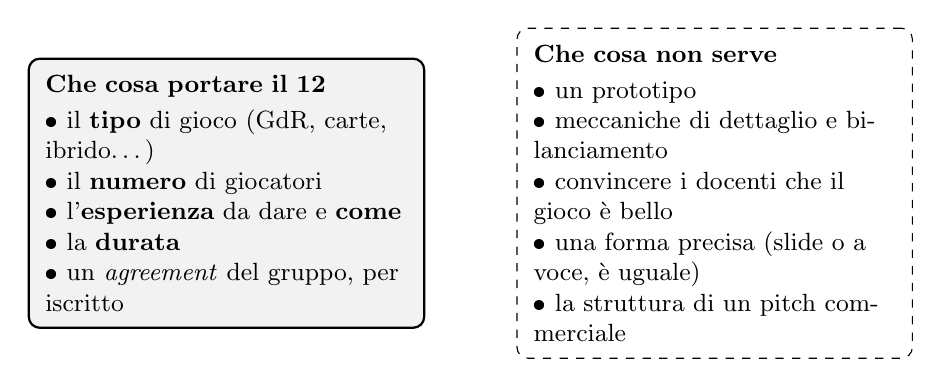
\begin{tikzpicture}[
    font=\small,
    si/.style={draw, thick, rounded corners, text width=4.6cm, align=left,
      fill=gray!10, inner sep=6pt},
    no/.style={draw, dashed, rounded corners, text width=4.6cm, align=left,
      fill=white, inner sep=6pt}
  ]
  \node[si] (a) at (0,0) {\textbf{Che cosa portare il 12}\\[2pt]
    \textbullet\ il \textbf{tipo} di gioco (GdR, carte, ibrido\ldots)\\
    \textbullet\ il \textbf{numero} di giocatori\\
    \textbullet\ l'\textbf{esperienza} da dare e \textbf{come}\\
    \textbullet\ la \textbf{durata}\\
    \textbullet\ un \emph{agreement} del gruppo, per iscritto};
  \node[no] (b) at (6.2,0) {\textbf{Che cosa non serve}\\[2pt]
    \textbullet\ un prototipo\\
    \textbullet\ meccaniche di dettaglio e bilanciamento\\
    \textbullet\ convincere i docenti che il gioco è bello\\
    \textbullet\ una forma precisa (slide o a voce, è uguale)\\
    \textbullet\ la struttura di un pitch commerciale};
\end{tikzpicture}
\caption{Il ``pitch'' del 12 ottobre come lo descrive Ruggero all'inizio della
lezione: un accordo sul \emph{che cosa}, non una vendita. Ricostruzione schematica.}
\label{a8:fig:pitch}
\end{figure}

% ---------------------------------------------------------------------
\section{Il programma: le mani nel motore}
\label{a8:sec:programma}

``Oggi, a livello logistico, vi dico cosa andiamo a fare''. Oggi è la lezione su
\textbf{Tabletop Simulator}: ``lavorare mani nel motore''. Il software va tenuto
aperto per tutta la lezione; chi non l'ha ancora installato lo installi subito (``non
è pesante, dovreste averlo pronto per tra 4 o 5 minuti''). Ci saranno domande e
momenti in cui chiedere di ``fermarmi a rispiegare una cosa'': ``fatelo, perché sono
qui apposta''.

\paragraph{Che cosa si dà per scontato.} Il software ``nasce per prototipare e
giocare'' giochi da tavolo. Ruggero dà per scontato che gli studenti l'abbiano già
usato \textbf{da giocatori} (\emph{user}, ``proprio di \emph{player}''), magari
giocando tra loro qualcosa che piace: serve ``il minimo necessario del sapersi
spostare all'interno del software'', cioè muovere la telecamera, cliccare sui menu,
sapere che cosa fanno i menu. Sono tutte cose che, come detto nel tutoraggio, ``il
tutorial di base vi spiega in 10 minuti''. Più complesso è \textbf{creare i moduli},
ed è quello che si fa oggi.

\paragraph{``Sì, ma con un asterisco''.} Tabletop Simulator è ``un software
gigantesco'' ed è impossibile coprirlo tutto in una lezione. Ruggero coprirà le
\textbf{basi} e lascerà l'ultima parte ai bisogni degli studenti: domande come ``si
può fare questa cosa qua su Tabletop Simulator?''. La risposta, ``come sempre, è quasi
sempre sì'': ``si può fare, con un asterisco: ma con un compromesso''. Il resto della
lezione spiegherà che cosa vuol dire.

Ruggero tiene il registro delle presenze in vista (``se per caso entra anche Giordano,
avvisatemi'') e condivide \textbf{tutto lo schermo}, non solo la finestra, perché
altrimenti i \emph{pop-up} del software non si vedono. Avverte che il programma, ``se
non l'avete mai aperto prima, può essere abbastanza ostile all'inizio''; ma alla fine
sarà chiaro perché è ``usatissimo nel settore'', e che ``non dovete stare 3000 ore per
saperlo usare bene''.

% ---------------------------------------------------------------------
\section{Avviare il software e creare una stanza}
\label{a8:sec:avvio}

Si lancia Tabletop Simulator da \textbf{Steam}. All'avvio il programma può proporre
un'opzione di lancio: giocare normalmente o avviare in modalità VR. Si sceglie il
gioco normale: ``è possibile usarlo con i set di realtà virtuale'', ma ``non siamo qua
per usare Tabletop in modalità VR''.

\paragraph{Il menu iniziale.} Nel menu si sente ``una musichetta fastidiosa'': si
toglie dall'ingranaggio, alla voce dei suoni, abbassando il volume del menu, ``così
magari riuscite anche a sentirmi senza impazzire''. L'icona della \textbf{lampadina}
apre il \textbf{tutorial} di base: ``io spero che voi l'abbiate già fatto. Se non
l'avete fatto, non ditemelo. Fatelo dopo la lezione senza dirmi niente, e io farò finta
che voi l'abbiate già fatto''. Poi ci sono le due voci grandi:
\begin{description}
  \item[Join] serve a unirsi a una partita che un'altra persona ha aperto; gli
        studenti dovrebbero già conoscerla, se hanno giocato con persone amiche.
  \item[Create] è quella che serve oggi: crea una partita \textbf{single player}, una
        \textbf{multiplayer} o una \textbf{hot seat}. L'\emph{hot seat} si ignora
        (``non la usa credo nessuno su questo pianeta, mai''). Il
        \emph{multiplayer} serve a creare partite con altri. Il \emph{single
        player} crea stanze in cui può entrare solo chi le crea, ed è quello che si
        usa per \textbf{costruire i moduli}.
\end{description}

\paragraph{I moduli si costruiscono in single player.} Ruggero è esplicito: ``non
create i moduli in multiplayer''. In multiplayer, del resto, solo l'\emph{host} può
crearli; ma soprattutto in single player è più comodo, perché ``la connessione
internet non vi chiederà costantemente il ping dei vostri compagni di stanza''.

All'apertura della stanza compare un \emph{pop-up} centrale, perché Tabletop
Simulator ``dà per scontato che noi vogliamo giocare qualcosa, non che vogliamo
creare un modulo''. Si chiude. Si resta con \textbf{un tavolo vuoto}, un panorama di
sfondo scelto a caso da un insieme predefinito e svariati menu. ``E a questo punto ci
dobbiamo chiedere: ok, benissimo. Cosa facciamo adesso?''.

% ---------------------------------------------------------------------
\section{``Un gioco da tavolo è un gioco su un tavolo''}
\label{a8:sec:simulatore}

Si parte ``dalle basi, proprio basi, basi''. Ruggero avverte che la lezione sarà
``piena di banalità'': frasi che suonano banalissime, ma che nell'ottica di Tabletop
Simulator ``non sono così banali''. E ripete un'informazione che era già stata messa
lì, ``nascosta, per fare \emph{foreshadowing}'', e che ripeterà ``fino allo
sfinimento'':

\begin{quote}
\textbf{Tabletop Simulator non è un software per fare videogiochi.} Non uscirete da qua
con il videogioco del vostro gioco da tavolo. Non vi serve a quello. Tabletop
Simulator, come il nome fa intuire, è un simulatore di giochi \emph{tabletop}. Vuol
dire che tutto quello che vedrete qua è \textbf{simulato fisicamente}: con un peso,
con una massa, con uno spazio, con delle collisioni.
\end{quote}

È il principio che regge tutta la lezione, e Ruggero lo riprenderà ogni volta che un
componente si comporta in modo inatteso: un mazzo che sul bordo del tavolo resta
inclinato, un cubetto che rotola giù dalla cornice di una plancia, una carta bucata
che però collide come se fosse intera. ``Questo è un simulatore di spazio fisico.
Spero che, se c'è una cosa che vi entra da oggi, è questa''. La conseguenza pratica:
i componenti di un modulo \textbf{vanno trattati come componenti fisici}, con le
stesse attenzioni che si avrebbero su un tavolo vero.

\paragraph{Approfondimento: il prototipo come simulazione.} La distinzione di Ruggero
tra \emph{simulatore} e \emph{motore} è la stessa che separa un prototipo di un gioco
da tavolo dalla sua versione digitale. Un adattamento digitale \emph{applica} le
regole al posto dei giocatori; un simulatore fisico, invece, lascia le regole ai
giocatori, come il tavolo vero, e si limita a riprodurre gli oggetti. È proprio questo
che lo rende adatto al \emph{playtest}: Schell, in \emph{The Art of Game Design},
insiste che ogni prototipo deve rispondere a una domanda precisa, e che la sua
fedeltà va scelta in funzione di quella domanda. Un prototipo su TTS risponde bene
alle domande su regole, spazio e flusso del turno, perché i giocatori devono ancora
eseguire tutto a mano, come farebbero con la scatola; risponde male, per costruzione,
alle domande che riguardano la manualità e il tatto. Il divieto degli \emph{script}
che Ruggero darà a fine lezione (sezione~\ref{a8:sec:script}) nasce dalla stessa
logica.

% ---------------------------------------------------------------------
\section{Il tavolo e la table presence}
\label{a8:sec:tavoli}

Nel menu in alto c'è la voce \textbf{Oggetti}, con quattro sottomenu:
\textbf{componenti}, \textbf{tavoli}, \textbf{background} e \textbf{oggetti
salvati}. Si parte dal tavolo.

\paragraph{Non tutti i giochi stanno su tutti i tavoli.} Nella vita reale, ``nella vita
di tutti i giorni, fisicamente'', alcuni giochi da tavolo su alcuni tavoli non si
possono giocare. Su un tavolino da caffè ``non ci sta probabilmente tutto
\emph{Twilight Imperium}''; sui tavolini del treno non ci si gioca un
\emph{eurogame}, ``perché il tavolo è più piccolo''. Allo stesso modo, quando si pensa
alla \textbf{table presence} del proprio gioco, cioè allo \textbf{spazio che occupa sul
tavolo}, la scelta non è casuale: non lo è nel mondo reale e non lo è su Tabletop
Simulator, perché lo spazio fisico è limitato: ``le cose che non sono sul tavolo
cadono dal tavolo''.

Il software offre \textbf{dieci tavoli}. Ruggero li mostra uno per uno
(tabella~\ref{a8:tab:tavoli}), guardando ogni volta due cose: quanti \textbf{posti}
ha e com'è fatto il \textbf{bordo}.

\paragraph{Le mani sono i posti a sedere.} Per contare i posti si usa, nel menu a
sinistra, la voce \textbf{Zone}, sottovoce \textbf{Hands}: mostra le \textbf{mani} di
carte, cioè le persone al tavolo. ``La \emph{hand} è in tutto e per tutto quanti
posti a sedere ci sono''. Se il tavolo ha quattro mani, ``questo gioco non può tenere
fisicamente più di quattro persone''; se si progetta un gioco da 6--8 persone, quel
tavolo ``già non va bene''.

\paragraph{Perché guardare i bordi.} ``So che vi sembra apparentemente inutile questa
informazione'', ma sopra il tavolo ci saranno dei componenti, e i componenti sono
oggetti fisici. Un bordo tridimensionale impedisce di tenere a bordo tavolo, ``belle
piatte, tranquille'', le plance dei giocatori; un rilievo al centro impedisce di
appoggiarvi piatta una plancia o un tabellone, perché ``questa salita qua è una
salita fisica che andrà a impattare i vostri componenti''.

\begin{table}[htbp]
\centering
\small
\begin{tabular}{@{}p{2.7cm}p{1.2cm}p{8.6cm}@{}}
\toprule
\textbf{Tavolo} & \textbf{Posti} & \textbf{Che cosa ne dice Ruggero} \\
\midrule
Square & 4 & piccolo, ``piccolino''; quattro persone ``strettine'' \\
Hexagon & 6 & un posto per lato, forma ``bizzarra''; \textbf{bordi
tridimensionali}: niente plance piatte a bordo tavolo \\
Octagon & 8 & come l'esagonale, con otto posti \\
Round & 8 & bordi molto meno marcati, ma al centro un \textbf{cerchio di vetro in
rilievo}: niente tabellone piatto al centro \\
Poker & -- & ``non vi servirà, a meno che non dobbiate fare poker'' \\
Rectangle & 8 & ``belli larghi''; bordi scanalati, ma superficie ampia: va bene per
``la maggior parte dei giochi pubblicati oggi'' \\
Round Glass & 8 & rotondo, grande, di vetro semitrasparente, con le gambe visibili
sotto, ``in stile Escher'': ``il tavolo peggiore di tutti. Non usatelo mai'' \\
Custom Rectangle & 8 & accetta un'immagine come superficie; il più grande; non se ne
sceglie la dimensione; l'immagine viene \textbf{stirata} \\
Custom Square & 8 & accetta un'immagine; gambe metalliche riflettenti; ``sembra
piccolo, ma è gigante''; nessun bordo strano \\
None & -- & nessun tavolo: i componenti ``cadono all'infinito in questo pozzo senza
fondo''. È l'opzione preferita di Ruggero, per un motivo che spiegherà dopo
(sezione~\ref{a8:sec:moduli}) \\
\bottomrule
\end{tabular}
\caption{I dieci tavoli di Tabletop Simulator come li presenta Ruggero. I nomi sono
quelli dell'interfaccia; i posti sono le \emph{hands} visibili nella voce
\emph{Zone}\protect\footnotemark.}
\label{a8:tab:tavoli}
\end{table}
\footnotetext{Per il tavolo da poker e per quello di vetro la trascrizione non riporta
il numero di posti (per il secondo dice solo ``per otto persone''). Il nome
``Round Glass'' per il tavolo di vetro è quello dell'interfaccia, che Ruggero non
pronuncia: lo descrive soltanto.}

\paragraph{Perché il software è fatto così.} Davanti al tavolo rotondo con il rilievo
al centro, la domanda viene da sé: perché qualcuno l'ha fatto? La risposta di Ruggero,
che tornerà molte volte nella lezione, è un misto di esasperazione e di affetto:
``perché sono pazzi'', ``è un miracolo che esista''. Chi ha creato il software ``non
sapeva cosa stava facendo''; oggi ci si ritrovano ``delle scelte vestigiali di gente
fulminata di anni fa che, contro la loro volontà, hanno purtroppo creato il software
di riferimento del settore, che è quello che tutti usano adesso''. E con queste scelte
``dobbiamo venire a patti''.

\paragraph{La scelta della lezione.} Per il prototipo dimostrativo Ruggero sceglie il
\textbf{tavolo quadrato custom} con una texture di legno: ``abbiamo un gioco piccolo,
magari un \emph{fillerino} per quattro persone, perfetto''. Sul tavolo senza tavolo
(\emph{None}) promette di tornare: ``ve lo spiego dopo, perché potrebbe essere
interessante''.

% ---------------------------------------------------------------------
\section{Caricare un'immagine: file locale e cloud}
\label{a8:sec:caricare}

Il tavolo \emph{Custom Rectangle}, appena selezionato, apre un \emph{pop-up} che chiede
un'\textbf{immagine}. È il primo incontro con una procedura che si ripeterà per quasi
ogni componente custom, e Ruggero ne fissa subito le due regole.

\paragraph{Regola 1: mai un URL, sempre un file.} Su Tabletop Simulator un oggetto
custom si può creare in due modi: dandogli l'\textbf{URL} di un'immagine online o
caricando un'immagine dal proprio computer (\textbf{Browse Local Files}). ``Il mio
consiglio personale è: non dategli mai un URL immagine'', perché se qualcuno, per
qualunque motivo, toglie quell'immagine dal suo indirizzo, ``il vostro modulo crolla''.
Se online c'è un'immagine che piace, la si \textbf{scarica} e la si ricarica dalla
propria cartella.

\paragraph{Regola 2: mai in locale, sempre in cloud.} Quando si carica un file, il
software chiede se caricarlo \textbf{in cloud} o \textbf{in locale}. ``Non caricate mai
niente del vostro modulo in locale'': un modulo con immagini locali non si può usare
in multiplayer, funziona solo sul proprio computer, e questo ``sconfigge un po'
l'obiettivo'' di farlo vedere, per esempio, a un \emph{publisher} esterno. Si carica
quindi in cloud, gli si può dare un nome, si aspetta che ``finisca di circolare questo
cerchiettino'' e si fa \textbf{Import}.

\paragraph{Le proporzioni.} Ruggero carica prima una texture di legno, poi un
tabellone più elaborato\footnote{La trascrizione descrive l'immagine come ``le
influenze moderne nella scena del Nord di Clarp'': con ogni probabilità è la
copertina o una pagina di un lavoro sul LARP nordico, usata a caso come esempio; il
contenuto dell'immagine non ha importanza.}: sul tavolo si può avere un tabellone,
uno schema, delle zone, ``già qualcosa di meccanico''. Ma la dimensione del tavolo non
si può definire: è il tavolo più grande che c'è, e l'immagine vi si adatta. Con una
texture verticale (una ``A'' arancione), il software ``la streccia come se non ci fosse
un domani'', e in più crea una luce arancione in faccia ``che sembra uscita da un film
sci-fi''. Quindi: \textbf{occhio alle proporzioni} delle immagini. Di solito il tavolo
si usa \textbf{con una texture}, e i tabelloni si mettono \textbf{a parte}, senza
caricarli direttamente sul tavolo, perché il tavolo li distorce.

% ---------------------------------------------------------------------
\section{Lo sfondo cambia la luce}
\label{a8:sec:sfondi}

Scelto il tavolo, Ruggero fa notare che la scena è buia: il suo sfondo è ``sera al
crepuscolo'', in mezzo a un prato, ``con tutto il problema di illuminazione che ne
deriva''. Il motivo è che Tabletop Simulator simula la \emph{skybox}, l'ambiente
attorno al tavolo. Dalla voce \textbf{Background} si sceglie lo sfondo: ``in questo
momento abbiamo il \emph{sunset}'', poi c'è il \emph{tunnel}, e così via.

Cambiando sfondo, Ruggero chiede di guardare il tavolo: che cosa succede? Uno studente
risponde: cambia il riflesso. Sì, e cambiano anche il livello di illuminazione e
l'angolazione. Non solo sulle gambe metalliche, che riflettono, ma anche sulla texture
di legno, che non è metallica: ingrandita, mostra colori ``più freddi, più caldi in base
a dove sono''. La luce, in Tabletop Simulator, arriva \textbf{da tre direzioni}:
\textbf{dall'alto}, \textbf{dall'orizzonte} e come \textbf{riflesso dal basso}. ``Stiamo
nel tecnico, mi rendo conto''; per ora il prato va benissimo. La questione tornerà con
il PDF, quando si vedrà che lo sfondo può rendere illeggibile un componente
(sezione~\ref{a8:sec:luce}).

% ---------------------------------------------------------------------
\section{I componenti: importare o creare?}
\label{a8:sec:componenti}

Abbiamo il tavolo, abbiamo lo sfondo, ``fantastico''. Ma mancano i componenti per
giocare. ``Vi sorprenderà sapere'' che dalla voce \textbf{Oggetti}, sottovoce
\textbf{Componenti}, si possono mettere dei componenti sul tavolo. I componenti sono
divisi in \textbf{16 categorie}, alcune più personalizzabili di altre. E l'approccio da
avere con questo software, per ogni pezzo del proprio gioco, è una domanda in due
tempi:

\begin{quote}
Devo importare un componente nel mio gioco? Ho qualcosa che mi può servire
\textbf{che già esiste}? O devo \textbf{crearlo da zero}?
\end{quote}

Ruggero passa quindi prima in rassegna i componenti ``più o meno standardizzati'' e il
modo di adattarli, e solo alla fine i componenti \emph{ad hoc}, i \textbf{custom}.

\subsection{Blocchi e cubetti}
\label{a8:sec:cubetti}

Nella categoria \textbf{Blocchi} ci sono un quadrato, un rettangolo e un triangolo; si
trascinano sul tavolo e si nota che sono \textbf{3D}. Rettangoli e triangoli per ora
non servono: si tengono i \textbf{cubetti}, una risorsa ``usatissima'' nei giochi da
tavolo. Ruggero chiede un esempio di gioco con i cubetti: gli studenti citano
\emph{Terraforming Mars} e \emph{Azul}\footnote{``Asol'' e ``terraform in Mars'' (poi
``terraform in Mark'') nella trascrizione. Ruggero aggiunge che in \emph{Azul} ci sono
``i cubetti neri per il contafonti'': il dettaglio non è ricostruibile con certezza
dalla trascrizione.}.

\paragraph{Ricolorare.} Il problema è che il cubetto è rosso, e nei giochi citati i
cubetti hanno altri colori. ``Ci può andare bene come forma, ma non come colore''. Per
ricolorarlo: \textbf{tasto destro}, \textbf{Color Tint}, e si sceglie il colore con la
classica barra di tonalità e saturazione, ``inclusa la semitrasparenza'': la barra in
fondo regola la trasparenza, e un cubetto blu con la barra abbassata diventa
semitrasparente. Un cubetto ``di grano'' si fa giallo, e così via.

\paragraph{Copiare.} Mentre si creano i moduli si possono usare \texttt{Ctrl+C} e
\texttt{Ctrl+V}: ``io posso copiarmi questi cubetti quanti ne voglio''.

\paragraph{Ridimensionare.} Un componente si può ingrandire o rimpicciolire dalla
tastiera, con i tasti \texttt{+} e \texttt{-}: per esempio un cubo più grande degli
altri, che valga tre o cinque risorse.

\subsection{Le dimensioni reali}
\label{a8:sec:misurare}

Il ridimensionamento serve per tutti i componenti, e qui Ruggero chiede di
``prepararsi psicologicamente'': quando si fanno moduli su Tabletop Simulator,
\textbf{è buona pratica mantenere le dimensioni e le proporzioni reali dei
componenti}. Ma come si sa quanto è grande un cubo? ``Può essere 10 cm, come 150, che
ne sappiamo''.

\paragraph{Lo strumento Linea.} Nel menu a sinistra c'è lo strumento \textbf{Linea}
(il righello). Nelle sue impostazioni si sceglie l'\textbf{unità}: Ruggero consiglia i
\textbf{centimetri} e la modalità 2D\footnote{La trascrizione rende le impostazioni
consigliate come ``2D free edge no log''; Ruggero dice di non volerle spiegare ``per
limiti di tempo'' e che ``centimetri, 2D'' è quello che serve. La forma esatta delle
altre voci non è ricostruibile dalla trascrizione.}. Con lo strumento si tira una
linea e il software scrive la misura sul bordo: il lato del cubo è ``più o meno 8
cm''.

\paragraph{Misurare dall'alto.} Per misurare con precisione si cambia prospettiva con
il tasto \texttt{P}, passando alla vista \textbf{dall'alto} (\emph{top-down}): senza
il problema del 3D si misura ``da un angolo all'altro''. Il lato risulta di 7 cm.
Se il cubetto dev'essere di 20 mm, lo si ridimensiona con \texttt{+} e \texttt{-}
finché la misura non è ``più o meno 2 cm''.

\paragraph{Una domanda di chiarimento.} Uno studente non ha capito: il cubo è stato
ridimensionato con la linea? No: il cubo si ridimensiona \textbf{con i tasti più e
meno}; la linea \textbf{misura} soltanto. Il tasto \texttt{Tab}, premuto una volta,
mette le freccette per indicare le cose; \textbf{tenuto premuto}, mostra la linea di
misura. Un'altra studentessa non ha capito come cambiare prospettiva: tasto \texttt{P},
``di prospettiva'', che passa tra prima persona, terza persona e vista dall'alto. Sono
cose che il tutorial dovrebbe aver già insegnato; in ogni caso, con il tasto
\texttt{Esc} si apre l'\textbf{Help}, con tutte le scorciatoie del software. Anche
spostare più componenti insieme e interagire con i componenti sono cose del tutorial.

\begin{figure}[htbp]
\centering
\begin{tikzpicture}[
    font=\small,
    passo/.style={draw, thick, rounded corners, text width=2.6cm, align=center,
      minimum height=1.3cm, fill=gray!10},
    freccia/.style={-{Stealth[length=2.5mm]}, thick}
  ]
  \node[passo] (a) at (0,0) {Linea: unità in \textbf{cm}, modalità \textbf{2D}};
  \node[passo] (b) at (3.3,0) {\texttt{P}: vista \textbf{dall'alto}};
  \node[passo] (c) at (6.6,0) {\texttt{Tab} tenuto premuto: \textbf{misura}};
  \node[passo] (d) at (9.9,0) {\texttt{+} / \texttt{-}: \textbf{scala} fino alla misura reale};
  \draw[freccia] (a) -- (b);
  \draw[freccia] (b) -- (c);
  \draw[freccia] (c) -- (d);
  \draw[freccia, dashed] (d.south) to[bend left=25] node[below, font=\footnotesize]
    {si rimisura finché non torna} (c.south);
\end{tikzpicture}
\caption{Come portare un componente alle sue dimensioni reali, secondo la procedura
mostrata da Ruggero: nell'esempio, un cubetto da 7 cm ridotto a 2 cm.}
\label{a8:fig:misurare}
\end{figure}

% ---------------------------------------------------------------------
\section{Le plance}
\label{a8:sec:plance}

La categoria \textbf{Board} contiene le \textbf{plance}: backgammon, scacchi o dama,
un'altra versione della scacchiera, dama cinese, Go, Reversi. ``La domanda però è:
perché ci sono?''. Il proprio gioco sarà sicuramente diverso da questi: quello che
serve, di solito, è la \textbf{Custom Board}, che chiede, ``indovinate un po''',
un'immagine, come il tavolo custom.

\paragraph{Bloccare la plancia.} La plancia si può spostare; con il tasto \texttt{L},
di \emph{lock}, la si \textbf{blocca}, in modo che cliccandoci sopra, anche per
sbaglio, non si sposti più. ``Questa è una buona pratica, perché noi non vogliamo che
qualcuno sposti il tabellone con tutte le cose sopra''.

\paragraph{La plancia si adatta all'immagine.} Uno studente nota che la plancia ha
cambiato dimensione da sola. Esatto: \textbf{al contrario del tavolo}, che adatta
l'immagine alla cornice (stirandola), \textbf{la board adatta la cornice
all'immagine}. Un'immagine alta dà una plancia stretta e alta; cambiandola (tasto
destro, \textbf{Custom}) con la texture del tavolo, la plancia si allunga dall'altro
lato. Ne segue una regola per i tabelloni: importarli \textbf{nelle proporzioni che
devono avere nella realtà}.

\paragraph{Il problema della cornice.} ``Ma adesso ti faccio vedere un'altra cosa''.
La plancia custom ha un \textbf{bordo di legno} in rilievo, ``nello stile delle vecchie
scacchiere''. E siccome i componenti sono 3D, un cubo appoggiato sul bordo
\textbf{rotola giù}. ``Quanti board game recenti avete visto con le plance che hanno la
cornice in legno alta due centimetri?''. Nessuno, risponde uno studente; ``forse una
versione super antica degli scacchi di mio nonno''. ``Esatto, perché è una roba da
fuori di testa'': nessuno mette una cornice di legno su un tabellone che costa 200
euro. La cornice non si può togliere. La soluzione arriverà più avanti
(sezione~\ref{a8:sec:tabellone}); per ora: ``tenetevi in background l'informazione''.

% ---------------------------------------------------------------------
\section{Le carte standard}
\label{a8:sec:carte-std}

La categoria \textbf{Carte} contiene: uno \emph{standard deck}, un \emph{custom deck},
una \emph{custom card}, una carta a caso (``randomicamente ci pesca una carta a
caso''), un \textbf{Jolly} (perché il mazzo standard è ``il classico deck da poker
normale di 52 carte'' e non ha i Jolly) e alcuni mazzi creati dagli autori di Tabletop
Simulator per un loro gioco, ``che non servono a niente di niente'': ``li lanciamo nel
sole''.

Come si interagisce con un mazzo (spostarlo, pescare, rivelare, pescare nella propria
mano) lo insegna il tutorial. Quello che importa sapere è che il mazzo \textbf{ha una
proprietà fisica}: la carta singola è più leggera del resto, il mazzo è
tridimensionale, e un mazzo appoggiato sul bordo del tavolo resta \textbf{inclinato},
tanto che si può vedere che cosa c'è sotto. ``Questo è un simulatore di spazio fisico.
Spero che, se c'è una cosa che vi entra da oggi, è questa''. I componenti ``vanno
trattati come se fossero componenti fisici''.

E se il gioco usa un mazzo di carte evento personalizzate? ``Ve lo spiego dopo'': prima
i componenti standard e come adattarli, ``e poi passiamo per ultimo ai componenti
\emph{ad hoc} vostri'' (sezione~\ref{a8:sec:mazzo}).

% ---------------------------------------------------------------------
\section{Dama, scacchi, dadi e figurine}
\label{a8:sec:dadi}

\paragraph{Dama e scacchi.} La quarta categoria sono i pezzi della \textbf{dama}, ``e
qui davvero abbiamo la follia di Tabletop Simulator'': c'è di nuovo la plancia,
identica a quella della categoria precedente, presente quindi in due categorie. Negli
\textbf{scacchi} ci sono pezzi metallici o di legno; ``se volete dei riflessi
ambientali, quelli di metallo sono perfetti''. Ma la domanda è sempre: servono?
Trattandosi di prototipi, se serve un pedone, ``nessuno si scandalizza se prendete un
pedoncino così e magari lo colorate, che so, rosso''.

\paragraph{I dadi.} Nella categoria \textbf{Dadi} ci sono dadi metallici e di plastica,
già colorati: d4, d6, d8, d10, d12 e d20, più altre versioni (per esempio d6 colorati
con gli angoli arrotondati). Si possono ricolorare e ingrandire: ``mi servono da 20,
ma blu''; lo si ricolora, lo si fa più grosso degli altri, e si tira come gli altri.
Ma attenzione: \textbf{ricolorare un componente non colora tutto}. Un dado bianco
colorato di giallo mantiene i \textbf{pallini} neri; un dado metallizzato colorato di
giallo ha i pallini bianchi, ed è \textbf{illeggibile}; un dado colorato di nero ``fa
schifo'', uno colorato di bianco è ``completamente illeggibile''. Quindi: attenzione a
quali componenti si scelgono come base.

\paragraph{Le figurine.} Nella categoria \textbf{Figurine} ci sono gli \emph{standee}
(le sagome in piedi) e le figurine metalliche, ``i classici omini di piombo'', che non
servono. Serve il \textbf{custom standee}, che chiede un'immagine di \textbf{fronte} e
una di \textbf{retro}. Ruggero vi mette la sua ``A'' davanti e dietro, ``ed ecco il
nostro standee''. Può essere un personaggio anche con la trasparenza: un PNG ritagliato
mantiene lo sfondo trasparente. Per avere un'immagine più grande mantenendo la base
piccola si usa il fattore di \textbf{scala}: con 2, l'immagine raddoppia e la base
resta piccola. ``Mi rendo conto che può essere estremamente noioso per ora questo
software''; tra poco arrivano ``le cose custom per davvero''.

% ---------------------------------------------------------------------
\section{Go, biglie, miscellanea}
\label{a8:sec:misc}

Ruggero passa ``velocissimamente'' sul resto.

\paragraph{Le pedine del Go.} Le pietre del Go ``possono essere come risorse'': si
vogliono risorse che siano sassolini, anziché cubetti? Benissimo. Colorate di azzurro
e rese semitrasparenti, diventano ``delle gocce d'acqua''.

\paragraph{Le biglie e i giochi di destrezza.} Le \textbf{biglie} sono biglie,
``letteralmente, con tutta la fisica che ne comporta'': su una superficie piana
continuano a rotolare. A che cosa servono? Ai \textbf{dexterity game}, i giochi di
destrezza, che si possono fare anche qui. La dimostrazione: Ruggero prende un
componente, lo mette sul tavolo e lo blocca; poi usa lo strumento \textbf{Flick} (il
``colpetto'' con il dito) sulla biglia, che va a sbatterci contro. ``Voilà! È un
simulatore fisico questo software''.

\paragraph{La miscellanea.} ``Dentro la miscellanea abbiamo tante cose bizzarre''.
\begin{itemize}
  \item Una \textbf{ciotola}: come componente non serve, ma bloccata sul tavolo e
        riempita di cubetti dà ``improvvisamente una \emph{table presence}
        diversa''.
  \item Una \textbf{moneta}, che lanciata dice testa o croce.
  \item Le pedine del \textbf{Reversi}, a due facce, una bianca e una nera: un
        \emph{token} a due lati già pronto.
  \item Pezzi del \textbf{domino}, tessere del \textbf{Mahjong}\footnote{``Testa del
        Maggiog'' nella trascrizione.}, altri dischetti, tutti ricolorabili, da
        usare come risorse.
  \item Un insieme di componenti dei designer del software\footnote{La trascrizione
        lo chiama ``P-Spec''; il nome della categoria non è ricostruibile con
        certezza.}: ``se vi servono, bene; se no, il mio sospetto è che non vi
        serviranno mai''.
  \item I \textbf{Player Pawn}, i classici pedoni di plastica, in \textbf{nove
        colori}. Perché nove versioni, se si possono ricolorare? ``Perché sono pazzi, i
        designer: non ci hanno pensato''. Ricolorateli come volete.
\end{itemize}

\paragraph{I colori dei giocatori.} C'è però una ragione per ricolorare con criterio.
Nel selettore dei colori, la colonna a destra contiene esattamente i \textbf{colori dei
giocatori}, cioè i colori delle mani attorno al tavolo\footnote{Ruggero dice prima
``questi 16 colori'' e poi ``esattamente i 12 colori player''; la trascrizione non
permette di stabilire quale dei due numeri sia quello inteso.}. Se si vuole un codice
colore preciso, legato al giocatore, si sceglie da lì: ``fammelo di questo arancione''
dà esattamente l'arancione del giocatore arancione.

\paragraph{Fiches e kit da GdR.} Poi le \textbf{fiches} da poker, ``classiche fiches
da casinò''; e il \textbf{RPG Kit}: miniature su miniature da \emph{dungeon crawler},
maghi, guerrieri, mostri, creature. ``Si muovono da sole queste'' (sono animate), ``un
po' anni Duemila, ma oh: per un prototipo su TTS, chi se ne frega?''.

\paragraph{Le cose ``fulminate''.} Infine la categoria preferita di Ruggero: ``le cose
così fulminate che mi fanno chiedere: ma perché, perché, perché hanno messo queste
cose qua? Non avremo mai una risposta''.
\begin{itemize}
  \item Una \textbf{Notecard}: un foglietto su cui si scrive con il tasto destro,
        compilando \textbf{nome} (il titolo) e \textbf{descrizione}. Si chiamano
        \textbf{index card}, ``usatissime per i giochi di ruolo in ambito americano,
        il \emph{tabletop} RPG specialmente''. Una studentessa si è persa: come si
        scrive? Tasto destro, e in fondo ci sono i due campi, nome e descrizione; si
        può andare a capo e mettere più righe; il testo ``non è in tempo reale'', si
        aggiorna solo quando si esce dal menu.
  \item Un \textbf{lettore MP3}: ``che devo dirvi? C'è un lettore MP3. Se volete
        giocare con la musica, ce l'abbiamo''. (Ruggero verifica che la classe senta
        l'audio del suo computer: ``vi voglio far soffrire per davvero''.)
  \item Un \textbf{contatore}, che si può far salire, scendere, azzerare, o in cui si
        scrivono direttamente i numeri.
  \item Un \textbf{tablet}, ``letteralmente un tablet'': ci si può aprire YouTube e
        guardare video. ``È un tablet, ragà, è un tablet. Non so che dirvi''.
  \item Una \textbf{sveglia} e una \textbf{calcolatrice}.
\end{itemize}

% ---------------------------------------------------------------------
\section{I sacchetti}
\label{a8:sec:sacchetti}

Nella miscellanea ci sono finalmente ``le due cose che ci servono per davvero'': il
\textbf{sacchetto infinito} e il \textbf{sacchetto}.

\paragraph{Il sacchetto infinito.} Parte vuoto e rende infinito qualunque cosa gli si
metta dentro: con un dado blu diventa un sacchetto infinito di dadi blu. Si può
ricolorare e si può azzerare (tasto destro, \textbf{Reset}) per farne, per esempio, un
sacchetto di dadi rossi. Ma Ruggero fa una richiesta precisa: \textbf{nei moduli per
questo corso non si usa il sacchetto infinito}, perché ``a livello produttivo io vi
chiederò quanti componenti avete, e infiniti non è un numero che è possibile stampare
nella realtà''. Per comodità è utilissimo, ``ma non è questo il momento''.

\paragraph{Il sacchetto normale.} Parte vuoto (passandoci sopra con il mouse si legge
zero) e ci si mette dentro qualunque cosa. Ruggero colora tre cubetti di giallo, rosso
e blu e li mette nel sacchetto; poi, con il tasto destro, decide \textbf{in che ordine}
il sacchetto restituisce gli oggetti (figura~\ref{a8:fig:sacchetto}):
\begin{description}
  \item[LIFO] (\emph{last in, first out}): l'ultimo oggetto messo è il primo a
        uscire. Messi blu, rosso, giallo, escono giallo, rosso, blu.
  \item[FIFO] (\emph{first in, first out}): il primo messo è il primo a uscire.
        Messi blu, rosso, giallo, escono blu, rosso, giallo.
  \item[Random]: ``è random''.
\end{description}
``Chiaramente non siamo persone fulminate'': un sacchetto, nella realtà, si comporta in
modo casuale, e quindi si mette \textbf{Random}. Nella prova, blu, rosso, giallo escono
giallo, rosso, blu.

\paragraph{Guardare dentro.} Per vedere che cosa c'è nel sacchetto: tasto destro,
\textbf{Search}. La stessa funzione si usa sui \textbf{mazzi}, per vedere le carte
rimaste.

\begin{figure}[htbp]
\centering
\begin{tikzpicture}[
    font=\small,
    cubo/.style={draw, minimum size=0.55cm, inner sep=0pt},
    etich/.style={font=\small\bfseries, anchor=east},
    freccia/.style={-{Stealth[length=2mm]}, thick}
  ]
  % ingresso
  \node[font=\footnotesize] at (0.9,1.9) {si inserisce};
  \node[cubo, fill=blue!40] at (0,1.3) {B};
  \node[cubo, fill=red!40] at (0.9,1.3) {R};
  \node[cubo, fill=yellow!50] at (1.8,1.3) {G};
  \draw[freccia] (2.3,1.3) -- (3.3,1.3);
  \node[draw, thick, rounded corners=6pt, minimum width=1.5cm, minimum height=1.2cm,
    align=center, font=\footnotesize] at (4.2,1.3) {sacchetto};
  % uscite
  \node[etich] at (7.2,2.2) {LIFO};
  \node[cubo, fill=yellow!50] at (7.7,2.2) {G};
  \node[cubo, fill=red!40] at (8.4,2.2) {R};
  \node[cubo, fill=blue!40] at (9.1,2.2) {B};
  \node[etich] at (7.2,1.3) {FIFO};
  \node[cubo, fill=blue!40] at (7.7,1.3) {B};
  \node[cubo, fill=red!40] at (8.4,1.3) {R};
  \node[cubo, fill=yellow!50] at (9.1,1.3) {G};
  \node[etich] at (7.2,0.4) {Random};
  \node[cubo] at (7.7,0.4) {?};
  \node[cubo] at (8.4,0.4) {?};
  \node[cubo] at (9.1,0.4) {?};
  \draw[freccia] (5.1,1.3) -- (5.5,2.2);
  \draw[freccia] (5.1,1.3) -- (5.5,1.3);
  \draw[freccia] (5.1,1.3) -- (5.5,0.4);
  \node[font=\footnotesize] at (8.4,2.8) {ordine di uscita};
\end{tikzpicture}
\caption{Le tre modalità del sacchetto, con l'esempio di Ruggero: tre cubetti
inseriti nell'ordine blu, rosso, giallo (B, R, G). Per un gioco da tavolo si usa
\emph{Random}, che è il comportamento di un sacchetto reale.}
\label{a8:fig:sacchetto}
\end{figure}

\paragraph{Approfondimento: il prototipo e la produzione.} La richiesta di non usare il
sacchetto infinito anticipa un tema che il corso affronterà con la lezione sulla
produzione: un gioco analogico è anche una \textbf{distinta dei componenti}, e ogni
componente ha un costo. Un modulo che usa scorte infinite nasconde al designer la
domanda ``quanti me ne servono davvero?'', che in un gioco stampato ha sempre una
risposta. Lo stesso vale per i cubetti copiati a volontà con \texttt{Ctrl+V}: comodi
per costruire, ma da contare prima di consegnare.

% ---------------------------------------------------------------------
\section{I componenti custom}
\label{a8:sec:custom}

``Allora, adesso arriviamo alla parte più incubo di tutte, che è la parte custom''. La
categoria \textbf{Custom} raduna tutte le opzioni personalizzabili, comprese quelle già
viste (la plancia, le figurine). Sono dieci (tabella~\ref{a8:tab:custom}).

\begin{table}[htbp]
\centering
\small
\begin{tabular}{@{}p{2.6cm}p{10.0cm}@{}}
\toprule
\textbf{Componente} & \textbf{A che cosa serve e che cosa ne dice Ruggero} \\
\midrule
Custom Board & una plancia da un'immagine; la cornice si adatta all'immagine, ma ha
il bordo di legno (sezione~\ref{a8:sec:plance}) \\
Custom Figurine & lo \emph{standee} con fronte e retro (sezione~\ref{a8:sec:dadi}) \\
Custom PDF & il \textbf{regolamento} del gioco, consultabile sul tavolo \\
Custom Token & un gettone con \textbf{forma libera} (gestisce la trasparenza e la
collisione), colorabile, impilabile; il retro è specchiato \\
Custom Tile & una tessera di \textbf{forma regolare} (quadrata, esagonale, circolare,
arrotondata) con fronte e retro corretti \\
Custom Deck & un \textbf{mazzo} di carte da una griglia di immagini: ``la parte più
difficile di tutte'' \\
Custom Card & una carta singola, fronte e retro \\
Custom Dice & un dado con le facce personalizzate, da un \emph{template} \\
Custom Model & un modello 3D (mesh, texture, collider): non si vede a lezione \\
Custom AssetBundle & pacchetti di modelli 3D, per esempio miniature: non si vede a
lezione \\
\bottomrule
\end{tabular}
\caption{I dieci componenti della categoria \emph{Custom}, come Ruggero li elenca
(``board, tile, token, figurine, deck, card, dice, model, asset bundle, PDF''). Modelli
3D e asset bundle in fase di prototipo sono fortemente sconsigliati.}
\label{a8:tab:custom}
\end{table}

% ---------------------------------------------------------------------
\section{Il PDF del regolamento e la luce}
\label{a8:sec:luce}

\paragraph{Caricare un PDF.} Il \textbf{Custom PDF} chiede di caricare un PDF. Ruggero
ne carica uno a caso, ``così a caso'': un PDF sul \emph{framework} DPE\footnote{``DPA
Framework'' nella trascrizione; con ogni probabilità il materiale sul framework DPE
(\emph{Design, Play, Experience}) visto nelle lezioni precedenti.}. ``Sempre
aspettare che finisca questa rondella blu, se no TTS impazzisce''. Il PDF appare sul
tavolo: è \textbf{molto piccolo} ed è \textbf{molto bianco}, quasi illeggibile, perché
l'illuminazione dello sfondo ``fa schifo''. Ed ecco il punto chiave sugli sfondi,
``lasciato in sospeso'' fino ad ora: cambiando lo sfondo cambia tutto. Ma magari non si
vuole giocare ``con le vibes di un pub di fumatori incalliti''.

\paragraph{Uno sfondo da un pixel.} Nel menu degli sfondi c'è un'opzione che Ruggero
aveva taciuto apposta: \textbf{Custom}, che permette di scegliere uno sfondo proprio.
Tabletop Simulator usa per gli sfondi panorami HDRI da $4000\times2000$ pixel, in un
formato specifico; ``ma non ce ne frega niente, perché in realtà noi possiamo fregare il
sistema'': come sfondo si può dare un'immagine di \textbf{un pixel per un pixel},
monocromatica, e si ottiene uno sfondo monocromatico attorno al tavolo. Ruggero ne ha
già preparati alcuni: dal menu \textbf{Modding}, alla voce \textbf{Cloud Manager}, si
vede tutto quello che si è caricato in cloud (``utile anche a voi per sapere cosa avete
caricato''), e lui ha una cartella di immagini utili con, tra l'altro, uno sfondo nero
da un pixel, ``leggerissimo da caricare''. Copiato e incollato nel \emph{Custom
Background}, il tavolo si ritrova ``in un nulla cosmico''. Ma la luce non cambia
ancora: è ancora quella dello sfondo precedente.

\paragraph{Le impostazioni di luce.} Dal menu \textbf{Options} si apre la voce
\textbf{Lighting}. La prima cosa da fare è \textbf{slegare la luce dallo sfondo}
(c'è una spunta apposta) e scegliere il \textbf{gradiente}: la visibilità migliora
subito. Poi Ruggero va ``voce per voce'' (tabella~\ref{a8:tab:luce}): ``so che vi
sembra complessa questa roba qui, ma non vi servirà sapere tutto''.

\begin{table}[htbp]
\centering
\small
\begin{tabular}{@{}p{3.4cm}p{9.2cm}@{}}
\toprule
\textbf{Voce} & \textbf{Che cosa fa e come impostarla} \\
\midrule
Luce legata allo sfondo & da \textbf{togliere}, scegliendo il gradiente \\
Light Intensity & la luce \textbf{dall'alto}, verticale: alta ``brucia tutto'', bassa
``non si vede niente''; di solito verso il fondo della barra, ma non al minimo \\
Light Color & di default una luce calda, un bianco non puro: ``lasciate questa, è una
buona luce'' \\
Ambient Intensity & la luce \textbf{laterale}, dell'ambiente: cambia i bordi degli
oggetti, non la faccia superiore; va bilanciata con la precedente ``in modo che non vi
faccia sputare gli occhi'' \\
Gradient Color (Sky, Equator, Ground) & ``non toccateli'' \\
Reflection Intensity & quanto riflettono i componenti \textbf{metallici} (tavolo,
dadi, pezzi): abbassata, il tavolo di metallo ``non riflette più niente'' e un dado
metallico diventa opaco \\
LUT e voci successive & ``ignorate queste cose, per carità. Non apriamo questo vaso
di Pandora'' \\
\bottomrule
\end{tabular}
\caption{Le impostazioni di luce di Tabletop Simulator (menu \emph{Options},
\emph{Lighting}) con i consigli di Ruggero\protect\footnotemark.}
\label{a8:tab:luce}
\end{table}
\footnotetext{La trascrizione rende l'ultima voce come ``loot loot contribution'' e
``Gaston, loot''; dovrebbe trattarsi delle impostazioni della LUT (\emph{look-up
table}), la tabella di correzione del colore. Ruggero aggiunge che chi è appassionato
di grafica 3D può andare a vederle ``in privato''.}

\paragraph{Come si vede la differenza.} Per mostrare la differenza tra le due
intensità, Ruggero porta prima al massimo e poi al minimo l'\emph{ambient intensity}:
``sembrano simili, ma non lo sono''. Il trucco è guardare un cubetto giallo: cambiando
la \emph{light intensity}, i colori dei \textbf{bordi} restano uguali, perché è la luce
verticale; cambiando l'\emph{ambient intensity}, che è la luce laterale, la faccia
\textbf{superiore} resta uguale. Per la \emph{reflection intensity} Ruggero cambia
tavolo (``lasciamo stare che sono volati via 38 componenti insieme, perché il tavolo
l'ho rimpicciolito'') e mostra che cambiano solo i componenti metallici, ``dadi inclusi'':
un dado ``nato metallico'' sembra cambiare colore e diventa ``bello matte''.

\paragraph{Il regolamento sul tavolo.} Tornando al PDF: lo si sfoglia con le
freccette, lo si ingrandisce, lo si mette a schermo. ``Questo è come importiamo i
regolamenti dei nostri giochi'': se il gioco ha un regolamento in PDF, si carica con il
Custom PDF, ``pulito, liscio, limpido, lampante''.

\paragraph{Modelli e asset bundle: no.} \textbf{Custom Model} e \textbf{Custom
AssetBundle} servono a caricare modelli 3D personalizzati, per esempio miniature. Non
si vedranno a lezione e non servono in fase di prototipo: ``non solo non vi verrà
richiesto, ma vi verrà fortemente incentivato a non usarli, a meno che non abbiate
proprio un obbligo particolare''.

% ---------------------------------------------------------------------
\section{Token e tile}
\label{a8:sec:token}

\paragraph{Che cos'è un token.} ``Sapete cos'è un token?''. ``So che sembra una risposta
banale, ma ci aiuta''. Una studentessa risponde: sono ``tipo quelle monetine che
c'erano in alcuni giochi''. Sì, per esempio; ma fisicamente che cos'è? Un gettone, sì,
e di solito è qualcosa che viene \textbf{estratto da una fustella}, una
\emph{punchboard}: nei giochi da tavolo i token sono pezzi di cartone fustellato. ``Se
avete comprato un gioco da tavolo nuovo, probabilmente li avete visti: li spingete via
con le manine ed estraete questi tokenini di cartone''. Su Tabletop Simulator è la
stessa cosa, solo che non li si estrae da una fustella.

\subsection{Il Custom Token}
\label{a8:sec:custom-token}

Ruggero crea un token con un'immagine qualunque, il logo di Audacity: ``voilà, abbiamo
il nostro token''. Le sue proprietà:
\begin{itemize}
  \item ha uno \textbf{spessore}, che dalle impostazioni custom si può aumentare (al
        massimo diventa ``un bel tokenone grosso'');
  \item si ridimensiona con \texttt{+} e \texttt{-}, come gli altri componenti;
  \item può stare \textbf{in piedi} anziché coricato (\emph{Stand Up}); ``notate che è
        molto strano, vedremo dopo perché'';
  \item può essere \textbf{impilabile} (\emph{Stackable}).
\end{itemize}

\paragraph{Impilabile o no.} La dimostrazione: due copie dello stesso token, una
normale e una impilabile. I token non impilabili messi uno sopra l'altro formano una
pila ``fisicamente'', ma ciascuno si sposta isolatamente. I token impilabili, invece,
vengono \textbf{impilati e contati} da Tabletop Simulator: passando sopra la pila con
il mouse, il software dice che è di 14 token.

\paragraph{Le proporzioni.} Il token \textbf{mantiene le proporzioni} dell'immagine: un
token da un'immagine rettangolare (una ``B'') è rettangolare, non viene stirato.

\paragraph{Il difetto: il retro è specchiato.} Quando si gira il token, la ``B'' è
\textbf{al contrario}. Con un token che porta delle scritte (Ruggero ne prende uno con
una scritta) il problema è evidente: girato, la scritta è rovesciata. E nelle opzioni
di importazione non c'è modo di dire ``non flipparmi il retro al contrario'': con il
Custom Token \textbf{non si può importare un componente con fronte e retro corretti}.

\subsection{Il Custom Tile}
\label{a8:sec:tile}

Per avere un retro corretto si usa il \textbf{Custom Tile}, la \textbf{tessera}. Chiede
cose simili ma non identiche: un'immagine \textbf{top} e un'immagine \textbf{bottom},
cioè che cosa c'è davanti e che cosa c'è dietro. Ruggero crea un tile con la stessa
immagine scritta del token e lo porta alla stessa dimensione, così da confrontarli.
Le differenze:
\begin{itemize}
  \item il token ha il bordo del colore del fronte, il tile ha il bordo
        \textbf{bianco};
  \item girati, il tile \textbf{mantiene la scritta corretta};
  \item il tile può avere un \textbf{retro diverso} dal fronte;
  \item il tile ha opzioni di \textbf{forma}: quadrato, \textbf{esagonale},
        \textbf{circolare}, \textbf{rounded} (rettangolare con i bordini
        arrotondati); il token non le ha.
\end{itemize}
``E quindi la domanda è: perché mai dovrei usare un token, quando posso usare un tile?''.

\paragraph{Il colore.} La prima risposta è il colore. Colorati entrambi di giallo (poi
di blu), il \textbf{tile} colora \textbf{solo il bordo}, mentre il \textbf{token} mette
un \textbf{filtro} colorato su tutta l'immagine. Quindi, se si vogliono tre token con
la stessa immagine, uno rosso, uno giallo e uno blu, il token permette di colorarli; e
su un'immagine bianca il colore viene applicato preciso (un rettangolo bianco colorato
di bianco resta il colore di base).

\paragraph{La trasparenza.} La seconda risposta è la trasparenza. Il token permette di
creare segnalini con la \textbf{trasparenza}, cioè \textbf{forme personalizzate}; il
tile la trasparenza non la gestisce, e la stessa immagine darà sempre una tessera con lo
sfondo bianco. Da cui la regola (tabella~\ref{a8:tab:token-tile}): \textbf{forma
custom, token; forma regolare (circolare, quadrata, arrotondata), spesso è più comodo
il tile}. ``Se avete dubbi o domande, vi prego, chiedetele, perché da adesso in poi
questo software fa solo che complicarsi la vita''.

\begin{table}[htbp]
\centering
\small
\begin{tabular}{@{}p{3.6cm}p{4.4cm}p{4.4cm}@{}}
\toprule
 & \textbf{Custom Token} & \textbf{Custom Tile} \\
\midrule
Forma & libera, dalla trasparenza del PNG & regolare: quadrata, esagonale,
circolare, arrotondata \\
Trasparenza & sì & no (sfondo bianco) \\
Retro & lo stesso del fronte, \textbf{specchiato} & immagine \emph{top} e
\emph{bottom}, corretta e anche diversa \\
Colore (Color Tint) & filtro su tutta l'immagine & solo il bordo \\
Bordo & del colore del fronte & bianco \\
Altre opzioni & spessore, \emph{Stand Up}, \emph{Stackable} & spessore, forma \\
Quando usarlo & segnalini sagomati, \emph{meeple}, standee, tabelloni (con
spessore minimo) & tessere, segnalini con scritte su entrambi i lati, plance \\
\bottomrule
\end{tabular}
\caption{Token e tile a confronto, secondo la dimostrazione di Ruggero.}
\label{a8:tab:token-tile}
\end{table}

\paragraph{Le sagome di persone.} Una domanda: le sagome di persone sono immagini
trasparenti fatte a token? Sì: nel Custom Token c'è l'opzione \textbf{Stand Up}, e con
un bordo un po' più ampio si ottiene una sagoma in piedi (``dev'essere molto grosso,
questo però, capiamoci''). Se il bordo è impreciso, è un lavoro ``di finezza'' sulla
\textbf{Merge Distance}: modificandola, il software ritaglia bordi più o meno accurati
in base a che cosa vede nell'immagine.

% ---------------------------------------------------------------------
\section{Il dado custom}
\label{a8:sec:dado}

``E ora arriviamo al punto che è traumatico. Ma ci siamo''. Mancano due componenti, il
\textbf{dado custom} e il \textbf{mazzo custom}.

\paragraph{Un'immagine per sei facce?} Il \textbf{Custom Dice} chiede prima che dado
si vuole (d4, d6, d8, d10, d12, d20), poi \textbf{un'immagine}. Una sola immagine per
sei facce? Che immagine? Provando con un'immagine a caso, il software la
\textbf{spalma} su tutto il dado. ``Al che la risposta è: Tabletop Simulator, che cosa
hai bevuto stasera? Come faccio a sapere che immagine devo caricare su questo dado?''.

\paragraph{I template nascosti.} La risposta sta nei file di installazione. Da
\textbf{Steam}: tasto destro su Tabletop Simulator nella libreria, \textbf{Proprietà},
\textbf{File installati}, \textbf{Sfoglia}. Si apre la cartella del software, e qui
l'avvertenza è perentoria: ``modificare questi file fa esplodere Tabletop Simulator.
Quindi non cancellate niente, non toccate niente''. Dentro c'è la cartella
\textbf{Modding}, con \emph{Deck Builder}, \emph{Deck Templates}, \emph{Dice
Templates} e altro. Nei \textbf{Dice Templates} ci sono le \textbf{UV map} dei dadi
(``maledetti, infami''\ldots).

\paragraph{Che cos'è una UV map.} Per chi non ha mai fatto modellazione 3D, Ruggero usa
un'immagine: i cioccolatini a forma di coniglio o di Babbo Natale avvolti nella carta
metallizzata. Srotolata, la carta è un'immagine piatta, ma avvolge una forma
tridimensionale. Allo stesso modo, il template è ``la carta che va messa attorno a
questo dado'': dice dove sono, nell'immagine piatta, le facce che interessano.

\paragraph{La procedura.} Si fa \textbf{una copia} del template del d6 (``non
modificate direttamente quel file, vi prego''), la si carica così com'è, ``e bum'':
il dado custom ha le facce di un d6 normale (``a questo punto usa il dado base, che era
anche meno brutto da vedere''). Ma l'immagine si può modificare, con Photoshop, GIMP,
``ma anche Paint''. Ruggero la apre con Paint e fa ``un lavoro approssimativo, fatto
davvero male, giusto per capirci'': i numeri pari rossi, i dispari verdi. Salva,
ricarica, ``e voilà: abbiamo il nostro bel dado. Bello è un eufemismo, chiaramente.
Brutto, ma ce l'abbiamo''. Le facce si possono quindi riempire di simboli o di
qualunque altra cosa.

\paragraph{Dov'è la cartella?} Uno studente si è perso: qual è la cartella? Ruggero
ripete: libreria di Steam, tasto destro su Tabletop Simulator, Proprietà, File
installati, Sfoglia; poi \emph{Modding} e \emph{Dice Templates}. ``Lo so, è brutto. È
così, va così''.

% ---------------------------------------------------------------------
\section{Il mazzo custom}
\label{a8:sec:mazzo}

``Ora arriva la parte più difficile di tutte, che purtroppo è quella più usata'': se si
fa un gioco da tavolo, di solito si fa un mazzo di carte personalizzato. ``Questa
parte qua è un inferno, ve lo dico per prepararvi psicologicamente''. Ruggero libera
metà del tavolo (``buttiamo tutto qua in alto, anche la ciotola'') e apre il
\textbf{Custom Deck}.

\subsection{Le opzioni di importazione}
\label{a8:sec:mazzo-opzioni}

Il software chiede, nell'ordine:
\begin{description}
  \item[La forma delle carte:] rettangolari con i bordi arrotondati, rettangolari
        senza, esagonali, circolari. Si lascia \emph{Rectangle (Rounded)}, ``le
        classiche da poker''.
  \item[La facciata] (\emph{Face}): l'immagine dei fronti.
  \item[Unique Backs:] se i retri sono \textbf{tutti uguali} (come nelle carte da
        poker) o se \textbf{ogni carta ha il suo retro}, come in certi giochi in cui
        ``un evento che puoi girare quando succedono cose ha dietro un evento
        diverso''. L'opzione più comune è nessun retro unico.
  \item[Il retro] (\emph{Back}).
  \item[Larghezza, altezza e numero:] \emph{Width}, \emph{Height} e \emph{Number}.
\end{description}

\paragraph{La griglia.} Le ultime tre voci non sono centimetri: sono numeri che vanno
da 2 a 10 (la larghezza), da 2 a 7 (l'altezza) e da 2 a 70 (il numero). Il motivo:
su Tabletop Simulator \textbf{ogni mazzo è una griglia di carte}, un'unica immagine
che le contiene tutte, e larghezza e altezza sono le dimensioni della griglia in
carte. Una griglia $5\times5$ contiene 25 posizioni, e nel numero si scrive
\textbf{24}.

\paragraph{Perché 24 e non 25.} Per ``motivi vestigiali'', \textbf{l'ultima posizione
della griglia non è usabile}: un tempo era usata per il retro, prima che venisse
aggiunta l'opzione del retro separato, e cambiare tutto ``farebbe saltare i vecchi
moduli''. Usarla dà problemi. Ne segue che il massimo di carte in un mazzo è
$10\times7-1 = \mathbf{69}$. Serve un mazzo più grande? Lo si importa in \textbf{due
mazzi separati} e poi li si mescola (figura~\ref{a8:fig:griglia}).

\begin{figure}[htbp]
\centering
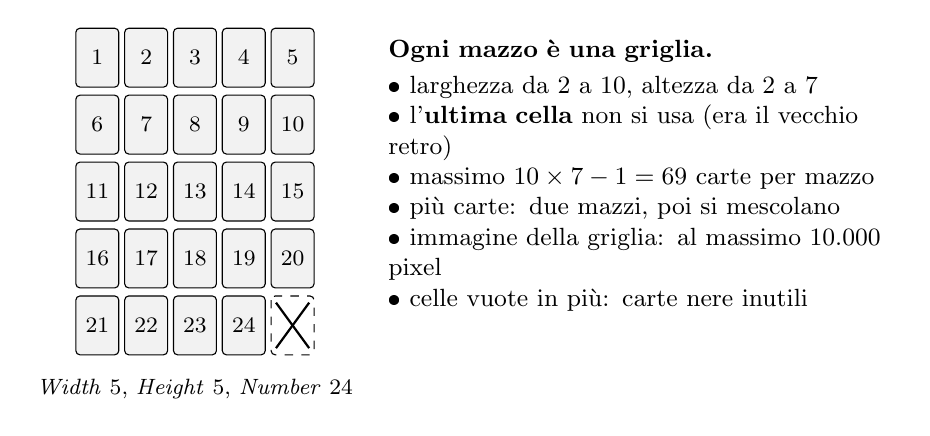
\begin{tikzpicture}[font=\footnotesize, x=0.62cm, y=0.85cm]
  % griglia 5x5
  \foreach \r in {0,...,4} {
    \foreach \c in {0,...,4} {
      \pgfmathtruncatemacro{\n}{\r*5+\c+1}
      \ifnum\n<25
        \draw[fill=gray!10, rounded corners=1.5pt] (\c,-\r) rectangle ++(0.88,-0.88);
        \node at (\c+0.44,-\r-0.44) {\n};
      \else
        \draw[dashed, fill=white, rounded corners=1.5pt] (\c,-\r)
          rectangle ++(0.88,-0.88);
        \draw[thick] (\c+0.1,-\r-0.1) -- (\c+0.78,-\r-0.78);
        \draw[thick] (\c+0.78,-\r-0.1) -- (\c+0.1,-\r-0.78);
      \fi
    }
  }
  \node[anchor=north, align=center] at (2.44,-5.1) {\emph{Width} 5, \emph{Height} 5,
    \emph{Number} 24};
  % nota a destra
  \node[anchor=west, text width=6.4cm, align=left, font=\small] at (6.2,-2.2) {
    \textbf{Ogni mazzo è una griglia.}\\[2pt]
    \textbullet\ larghezza da 2 a 10, altezza da 2 a 7\\
    \textbullet\ l'\textbf{ultima cella} non si usa (era il vecchio retro)\\
    \textbullet\ massimo $10\times7-1 = 69$ carte per mazzo\\
    \textbullet\ più carte: due mazzi, poi si mescolano\\
    \textbullet\ immagine della griglia: al massimo 10.000 pixel\\
    \textbullet\ celle vuote in più: carte nere inutili};
\end{tikzpicture}
\caption{La griglia di un mazzo custom nell'esempio di Ruggero: $5\times5$, con 24
carte e l'ultima cella inutilizzabile. Ricostruzione schematica.}
\label{a8:fig:griglia}
\end{figure}

\paragraph{I template dei mazzi.} Nella stessa cartella dei template dei dadi ci sono i
\textbf{Deck Templates}, con esempi di griglie (anche qui l'ultima carta non è usata).
Servono a poco: danno carte rettangolari e carte quadrate, ma ``che dimensione sono
queste carte? Io magari ho carte di dimensione diversa, strette e alte. Come
faccio?''. La griglia si può comporre a mano con qualunque programma, anche Photoshop,
mettendo le carte ``a manina una di fianco all'altra'', ``ma impazzite senza se e senza
ma''.

\subsection{Il Deck Editor}
\label{a8:sec:deck-editor}

Per questo, nella cartella \emph{Modding}, alla voce \emph{Deck Builder}, Tabletop
Simulator ha un \textbf{software secondario}: il \textbf{TTS Deck Editor}. Prima
pessima notizia: \textbf{non esiste per Mac}. ``Spero che abbiate dei compagni di gruppo
con Windows''. (E Ruggero ricorda che fare un gioco da tavolo non è obbligatorio:
``potete fare anche giochi pervasivi, LARP, giochi di ruolo''.)

Il Deck Editor ``è questa orripilezza qua, sembra fatto da un ingegnere''. La
procedura che Ruggero mostra (figura~\ref{a8:fig:mazzo}):
\begin{enumerate}
  \item \textbf{Nuovo mazzo}: il programma chiede larghezza e altezza della griglia,
        ``esattamente quelli che TTS ci chiede''. Ruggero sceglie $5\times5$. La
        griglia è ``grigia su grigia'', quindi non si vede (``un altro aspetto della
        brillantezza geniale dei programmatori''): compare solo quando ci si
        trascinano dentro le carte.
  \item Si \textbf{trascinano} le immagini delle carte nella griglia e le si copia
        quante volte serve. Nell'esempio: quattro copie dei numeri dal 2 al 6 e
        quattro Jack, ``a caso, non è un mazzo reale''.
  \item \textbf{File, Save Deck As}: si salva nella propria cartella di lavoro un file
        \texttt{.tsdb} (Ruggero lo chiama ``mazzo''). Ma Tabletop Simulator
        \textbf{non apre i \texttt{.tsdb}}: quel file serve solo a riaprire il mazzo nel
        Deck Editor.
  \item \textbf{File, Export}, con due accorgimenti: \textbf{togliere la spunta da
        Upload Image} (le immagini si caricano a mano, non online) e impostare
        \textbf{Max Deck Size a 10.000}. È ``una \emph{safety measure}'': se le carte
        sono gigantesche, il programma le ridimensiona in modo che la griglia non
        superi i 10.000 pixel, perché ``Tabletop Simulator crasha con le immagini più
        grosse di 10.000 pixel''. Si esporta e si ottiene \textbf{l'immagine della
        griglia}.
  \item In Tabletop Simulator, nel Custom Deck: l'immagine della griglia come fronte
        (in cloud), un retro generico (``questo blu mi va bene''), griglia $5\times5$,
        numero 24.
  \item \textbf{Sideways}: è un'opzione vestigiale, ``non spuntatela''; serviva ai
        vecchi mazzi, che non potevano avere carte orizzontali.
  \item \textbf{Backs is hidden}: \textbf{va spuntata}.
  \item \textbf{Import}, ``ed eccolo qua: abbiamo il nostro mazzo''.
\end{enumerate}

\paragraph{Backs is hidden e le mani.} Ruggero mostra a che cosa serve l'ultima spunta.
Dà delle carte alla propria mano e ad altre mani: le carte esistono, ma lui non vede
che cosa c'è nelle mani altrui. Cambiando colore e passando al giallo, vede il giallo e
non vede più l'arancione. \emph{Backs is hidden} significa questo: quando una persona
ha una carta in mano, quella carta è nascosta, e nelle mani degli altri si vede
\textbf{il retro} delle carte anziché il fronte.

\begin{figure}[htbp]
\centering
\begin{tikzpicture}[
    font=\small,
    passo/.style={draw, thick, rounded corners, text width=3.3cm, align=center,
      minimum height=1.25cm, fill=gray!10},
    file/.style={draw, dashed, rounded corners, text width=2.5cm, align=center,
      minimum height=0.8cm, font=\footnotesize},
    freccia/.style={-{Stealth[length=2.5mm]}, thick}
  ]
  \node[passo] (a) at (0,0) {\textbf{Deck Editor}\\ nuovo mazzo, griglia $W\times H$};
  \node[passo] (b) at (4.2,0) {trascinare e copiare le \textbf{carte}};
  \node[passo] (c) at (8.4,0) {\textbf{Export}: niente Upload Image, Max Deck Size
    10.000};
  \node[passo] (d) at (8.4,-2.4) {\textbf{TTS}, Custom Deck: fronte (cloud), retro,
    $W$, $H$, numero};
  \node[passo] (e) at (4.2,-2.4) {Sideways \textbf{no}, Backs is hidden
    \textbf{sì}, Unique Backs se serve};
  \node[passo] (f) at (0,-2.4) {\textbf{Import}: il mazzo è sul tavolo};
  \node[file] (s) at (4.2,1.6) {\texttt{.tsdb}: si riapre solo nel Deck Editor};
  \draw[freccia] (a) -- (b);
  \draw[freccia] (b) -- (c);
  \draw[freccia] (c) -- (d);
  \draw[freccia] (d) -- (e);
  \draw[freccia] (e) -- (f);
  \draw[freccia, dashed] (b) -- node[right, font=\footnotesize] {Save Deck As} (s);
\end{tikzpicture}
\caption{Il flusso di lavoro per creare un mazzo custom, come lo mostra Ruggero. Il
file \texttt{.tsdb} conserva il mazzo per le modifiche successive; a Tabletop
Simulator serve l'immagine esportata.}
\label{a8:fig:mazzo}
\end{figure}

\subsection{Le domande di Gianmarco}
\label{a8:sec:mazzo-domande}

\paragraph{Gli angoli arrotondati.} Gianmarco si è perso una cosa: l'arrotondamento
degli angoli delle carte l'ha fatto Ruggero nelle immagini? Sì e no. Ruggero ha
scaricato da internet un kit di carte singole, ``ce ne sono mille online'', già con gli
angoli arrotondati; ma nelle opzioni custom le carte sono impostate come arrotondate.
Impostandole rettangolari senza arrotondamento, gli angoli diventano neri, perché il
software riempie con il nero la trasparenza dell'immagine. Quando invece le si imposta
arrotondate, è il software ad arrotondarle ``a manina'', e infatti l'arrotondamento
del mazzo è un po' meno accentuato di quello delle immagini.

\paragraph{Più celle che carte.} ``È una domanda veramente stupida'': che cosa succede
se si mette una griglia $6\times6$ e poi un numero diverso dalle carte reali? Ruggero
lo mostra sul $5\times5$, impostando 35 carte: ``ti dà carte nere che non servono''.

\subsection{Carte con retri diversi}
\label{a8:sec:retri}

Finora le carte avevano tutte lo stesso retro. Per un mazzo in cui \textbf{ogni carta
ha il suo retro}: Ruggero copia il file \texttt{.tsdb} (``lo chiamo mazzo retro, così
lavoriamo su un mazzo diverso'') e vi compone la versione ``dark'' delle stesse carte,
nelle stesse posizioni (i numeri dal 2 al 6 neri, e il Jack). Nel Custom Deck, come
fronte resta la griglia di prima; come retro si carica la \textbf{seconda griglia, che
dev'essere identica} nella disposizione; si spunta \textbf{Unique Backs}. Importato, il
mazzo ha ``ognuna il suo retro''. È anche la risposta alla domanda di uno studente sulle
carte a doppia faccia, come quelle di \emph{Taboo}\footnote{``Tabu'' nella
trascrizione.}.

\subsection{La carta singola e le carte bucate}
\label{a8:sec:bucate}

\paragraph{La carta singola.} Il \textbf{Custom Card} chiede semplicemente fronte e
retro, ``senza tutto il resto''. Ruggero crea una carta con il re bianco davanti e il re
nero dietro: una carta singola, che si può mettere insieme alle altre.

\paragraph{Si possono bucare le carte?} Una studentessa chiede se le carte possono essere
forate, ``tipo una sorta di stencil''\footnote{La trascrizione dice ``una sorta di
stendarda'' e poi ``una sorta di scherzo''; dal seguito si capisce che si parla di
carte con dei fori, attraverso cui si vede ciò che sta sotto.}. Sì, perché Tabletop
Simulator gestisce la trasparenza. Ruggero copia il re, lo apre in Photoshop (``per
bucare le cose sono più comodo'') e ci fa un buco e un taglio scanalato di fianco;
basta un qualunque PNG con della trasparenza. Ricaricata, la carta \textbf{è bucata}:
si vede attraverso. ``Attenzione, però'': è bucata \textbf{l'immagine}, ma non è
bucata la \textbf{collisione}; un oggetto appoggiato sopra il buco non ci passa. E
il retro può anche non essere bucato: Ruggero ha bucato solo uno dei due lati, ``una
carta che non può esistere fisicamente''. La carta ha comunque uno spazio fisico che
non si può cambiare. Se si vogliono carte con uno \textbf{spazio fisico bucato}, si
usa il \textbf{token}, che gestisce la trasparenza \emph{anche} nella collisione: un
token ingrandito, appoggiato su un altro oggetto, non collide dove è trasparente.

% ---------------------------------------------------------------------
\section{Il tabellone senza cornice}
\label{a8:sec:tabellone}

Resta il problema della plancia con la cornice di legno
(sezione~\ref{a8:sec:plance}). ``Già lo sapete a questo punto come si fanno i
tabelloni'': \textbf{non li si importa come plance, li si importa come token}. Si crea
un token con una \textbf{profondità molto bassa}, gli si dà l'immagine del tabellone,
lo si ingrandisce in formato tabellone e lo si \textbf{blocca} sul tavolo. ``Anche se
tecnicamente, per TTS, è un token, questa per noi è una plancia''.

\paragraph{La prima pausa.} ``Ora vi darei forse dei minuti di pausa prima di passare
alla prossima fase, se vi va''. ``Se non è già troppo tardi, forse vi ho già consumato
troppo''. Pausa di sette minuti: si riprende alle \textbf{18:40}.

% ---------------------------------------------------------------------
\section{Penna, testo e fogli di carta}
\label{a8:sec:penna}

Al rientro Tiziana saluta (``nessun problema, Tiziana, va benissimo'') e, a quanto
si capisce, lascia la lezione. Ruggero riapre alle domande su quanto visto finora:
caricare componenti, aggiungerli al tavolo.

\paragraph{Esistono delle penne?} Una studentessa chiede se esistono delle penne, per i
giochi in cui bisogna appuntare dei punti o scrivere delle cose. Sì: c'è lo strumento
\textbf{Draw}, la penna, in alto a sinistra, di cui si può cambiare il colore e con cui
si disegna e si scrive sui componenti. (Ruggero si accorge di non aver ancora
ricondiviso lo schermo dopo la pausa: ``giustamente, se no non vedete''.) Ma la penna
non è un componente che si aggiunge: è uno degli \textbf{strumenti base} di TTS, come
il \emph{Grab} e lo strumento \textbf{Testo}. Sono strumenti usati solo nei giochi che
li richiedono, per esempio i \emph{party game} in cui si disegna.

\paragraph{Il foglio di carta.} Quello che manca è il foglio. Ma il foglio può essere
un \textbf{tile} o un \textbf{token bianco} su cui si disegna con la penna nera; oppure
si può usare una texture di carta. O, ancora, si apre un \textbf{tavolo custom} con una
texture bianca: allora ``tutto il tavolo è il nostro tabellone''.

% ---------------------------------------------------------------------
\section{Salvare e pubblicare il modulo}
\label{a8:sec:workshop}

Il modulo ha luce, tavolo, sfondo e componenti. Come lo si salva?

\paragraph{Save \& Load: solo in locale.} La prima opzione è nel menu \textbf{Games},
alla voce \textbf{Save \& Load}. Ruggero salva il modulo come ``Prototipo''; il
salvataggio compare nell'elenco e, cliccandoci, ricarica il modulo così com'era, anche
dopo aver cambiato stanza: ``si ricorda tutto quello che c'era''. Ma un salvataggio è
\textbf{usabile solo in locale}: non lo si può mandare a un \emph{publisher} perché lo
valuti. Per questo bisogna caricarlo come modulo sul \textbf{Workshop} di Steam, ``e
fare questa cosa è un po' più complesso''.

\subsection{Upload e Update}
\label{a8:sec:upload}

Dal menu \textbf{Modding}, la voce \textbf{Workshop Upload} apre una finestra con due
schede:
\begin{description}
  \item[Upload Workshop] si usa \textbf{solo la prima volta} che si carica il
        modulo;
  \item[Update Workshop] si usa per \textbf{tutti gli aggiornamenti} successivi, ``ed
        è più semplice''.
\end{description}

\paragraph{Le informazioni del modulo.} Prima di caricare conviene compilare le
\textbf{Info} del modulo (dal menu del gioco): nome, tipologia, complessità, tempo di
gioco, numero di giocatori, \emph{tag} del Workshop. ``Queste sono informazioni
meccaniche del Workshop''. Ruggero imposta: tipo \emph{game}, complessità bassa,
30--60 minuti, da 2 a 4 giocatori, nome ``prototipo brutto''. (Nel farlo, si accorge di
aver aggiunto per sbaglio un modulo: ``è un inferno, adesso''.)

\paragraph{Il caricamento.} Nell'Upload si scrivono il \textbf{titolo} (``prototipo
brutto''), una \textbf{descrizione} (``quello che volete, lasciamola uguale al
titolo'') e un'\textbf{immagine di anteprima}: ``mi sembra \emph{fitting} metterci la
texture del legno''. Si fa Upload; dopo qualche secondo compare in alto una scritta
verde: il modulo è caricato. Un \emph{pop-up} mostra un numero, l'identificativo del
Workshop, e raccomanda di conservarlo. ``Non ce ne frega niente'': si recupera quando
si vuole, ``non dobbiamo salvarlo o esplodere il mondo''.

\paragraph{La pagina del Workshop.} Nella libreria di Steam, su Tabletop Simulator, c'è
la voce \textbf{Workshop}; da lì, \textbf{i tuoi oggetti}, \textbf{oggetti
pubblicati}. C'è ``prototipo brutto'', con la sua pagina, ``esattamente come le
altre, solo che più brutta'', con il tasto \textbf{Iscriviti} come gli altri moduli.
In alto, però, c'è scritto che la visibilità attuale è \textbf{nascosta}: solo l'autore
può vederlo.

\subsection{La visibilità: unlisted}
\label{a8:sec:visibilita}

Dalla pagina si cambia la visibilità: \textbf{pubblico}, \textbf{solo amici},
\textbf{non in elenco} (\emph{unlisted}), \textbf{nascosto}. Le opzioni che servono sono
due; ``le altre sono delle mezze vie che non servono a nessuno''.
\begin{description}
  \item[Pubblico:] chiunque può entrare nel modulo, guardarlo, copiare le cose,
        prendere i componenti, salvarsi oggetti e immagini.
  \item[Unlisted:] lo vede solo chi riceve il \textbf{link diretto}. L'URL del modulo
        è in alto nella pagina; oppure, tasto destro sullo sfondo, \emph{Copia URL
        della pagina}.
\end{description}
\textbf{Per questo corso, i moduli si pubblicano unlisted}, ``se dovete farlo''. La
pagina del Workshop si può modificare come quelle degli altri giochi (Ruggero ne apre
una come esempio): descrizione, titolo, altre immagini, screenshot, ``paro paro''.

\begin{figure}[htbp]
\centering
\begin{tikzpicture}[
    font=\small,
    passo/.style={draw, thick, rounded corners, text width=2.7cm, align=center,
      minimum height=1.3cm, fill=gray!10},
    locale/.style={draw, dashed, rounded corners, text width=2.7cm, align=center,
      minimum height=1.3cm},
    freccia/.style={-{Stealth[length=2.5mm]}, thick}
  ]
  \node[locale] (s) at (0,1.8) {\textbf{Save \& Load}\\ \footnotesize solo sul proprio
    computer};
  \node[passo] (i) at (0,0) {\textbf{Info}: nome, tipo, complessità, tempo,
    giocatori};
  \node[passo] (u) at (3.5,0) {\textbf{Workshop Upload}: titolo, descrizione,
    anteprima};
  \node[passo] (p) at (7.0,0) {Steam: \textbf{pagina} del modulo (nascosto)};
  \node[passo] (v) at (10.5,0) {visibilità \textbf{unlisted}: si condivide il
    link};
  \node[locale] (up) at (3.5,-2.0) {\textbf{Workshop Update}\\ \footnotesize per ogni
    modifica successiva};
  \draw[freccia] (i) -- (u);
  \draw[freccia] (u) -- (p);
  \draw[freccia] (p) -- (v);
  \draw[freccia, dashed] (up) -- (u);
\end{tikzpicture}
\caption{Dal salvataggio locale al modulo condivisibile, secondo la procedura di
Ruggero. La prima pubblicazione si fa con l'Upload, tutte le successive con l'Update.}
\label{a8:fig:workshop}
\end{figure}

% ---------------------------------------------------------------------
\section{Prendere i componenti degli altri}
\label{a8:sec:riuso}

\paragraph{Save Object.} Una studentessa chiede: quindi chiunque potrebbe prendere i
componenti di altri giochi, se li si fa pubblici? ``Ah, sì, certo. Anzi, adesso arrivo
a parlarvi di questo''. Se serve un componente particolare trovato in un altro modulo,
lo si può salvare. Ruggero apre un modulo pubblico\footnote{``Farm Race'' nella
trascrizione: il titolo del modulo non è verificabile.} che ha dei token a forma di
animale e prende una \textbf{gallina}: tasto destro, \textbf{Save Object}, e la si
chiama ``gallina''. Tornati nel proprio modulo, dal menu Oggetti c'è l'ultima voce che
non aveva ancora nominato, \textbf{Oggetti salvati}: la gallina è lì. ``Così come io
ho salvato un granchio col coltello, per esempio. Può sempre essere utile''. ``Ho anche
un granchio senza coltello''.

\paragraph{Dove finiscono gli oggetti salvati.} Una studentessa ha salvato un mazzo di
carte, con immagini caricate da lei, ma non lo trova più. Se ha fatto un \emph{Save
Object}, dovrebbe trovarlo negli oggetti salvati; caricare le immagini da qualche parte,
da sola, non salva l'oggetto. In ogni caso, \textbf{tutto quello che si è caricato} è
nel menu \textbf{Modding}, alla voce \textbf{Cloud Manager}. È anche buona pratica
farci un po' di pulizia.

\subsection{Quando la sorgente sparisce}
\label{a8:sec:sorgente}

Gli oggetti salvati restano utilizzabili \textbf{finché chi ha caricato l'immagine la
tiene online}. Ruggero ha appena cancellato dal cloud un'immagine (una carta,
``lanciata nel sole'') e vuole mostrare che cosa succede: ricaricando il modulo
dovrebbero comparire degli errori. Ma sul suo computer non succede, perché le immagini
sono ancora nella \emph{cache}, e per svuotarla dovrebbe chiudere e riaprire il software
(``non ho voglia''). Allora condivide il link del Workshop perché qualcuno lo provi.

\paragraph{Discord, non la chat.} Prova a scrivere il link nella chat della lezione;
``No, su Discord, Ruggero, altrimenti non possiamo copiarlo e incollarlo''. Ha ragione:
gli anni scorsi non era così, ma la piattaforma ha cambiato le impostazioni di
sicurezza (``con la questione delle IA hanno aumentato le difese, ma verso cosa?
Comunque, questi sono i miei rant''). Uno studente vorrebbe provare a condividere lo
schermo, ma è collegato dal computer aziendale, che non gli permette di installare
Steam. Ruggero allora descrive l'effetto: chi carica un modulo a cui manca la sorgente
di un'immagine vede un \textbf{messaggio di errore rosso} in alto, ripetuto nella chat
del gioco, e il componente può non caricarsi affatto.

\paragraph{La gallina era un modello 3D.} Il caso della gallina è istruttivo. Aprendo
il suo menu custom, si scopre che non è un token: è un \textbf{modello 3D custom}, a cui
qualcuno ha dato una \textbf{mesh}, un'immagine \textbf{diffuse} e un \textbf{collider}.
Per non perderla, bisognerebbe salvare sul proprio computer queste tre cose
separatamente: ``roba da uscirci impazziti''. Quindi: \textbf{attenzione a che cosa si
salva}, e da dove viene.

\paragraph{I moduli di meeple.} Esistono però moduli che fanno ``il lavoro sporco'' per
gli altri. Ruggero ne usava uno ``che era una bomba atomica'', in cui qualcuno aveva
caricato più di cento modelli 3D di \emph{meeple} di forme diverse; lo riapre, il
software va in crash, e quando lo riapre davvero ne è sopravvissuta circa la metà:
``RIP''. Ma cercando ``meeples'' nel Workshop di Tabletop Simulator si trovano vari
moduli che hanno l'unico scopo di fornire segnalini di varie forme\footnote{La
trascrizione cita un modulo che rende con ``Wooden Talker'' e un altro, ``Mipolorama'',
probabilmente un gioco di parole su \emph{meeple}; i titoli esatti non sono
ricostruibili.}: un riccio, un omino col cappello, barche, camion, stivali, ``tutti
ricolorabili''. ``Avete l'imbarazzo della scelta''.

% ---------------------------------------------------------------------
\section{I moduli di Ruggero}
\label{a8:sec:moduli}

``Ora vi faccio vedere cosa si può fare su Tabletop Simulator quando si lavora per fare
dei moduli'': i moduli che Ruggero ha fatto in passato, ``dai più \emph{easy} ai più
complessi''.

\subsection{Un gioco di carte}
\label{a8:sec:mod-carte}

Il primo è un gioco ``molto \emph{card based}'' fatto per un lavoro\footnote{La
trascrizione dice ``quando lavoravo per Camon''; il nome del committente non è
ricostruibile.}. C'è il \textbf{regolamento} in alto, che si apre a doppia pagina;
\textbf{nove mazzi} di carte; un \textbf{tabellone} con i segnalini che segnano le
risorse e che \textbf{scattano in posizione} (``non stanno a metà via''); sacchetti con
i dadi; plance con i tracciati e i segnalini delle risorse. ``Liscio, regolare: tutte
cose che in teoria dovreste già saper fare anche voi''.

Ruggero ne approfitta per interrogare la classe:
\begin{itemize}
  \item La \textbf{bandiera}, che componente è? Un \textbf{token}, perché ha una forma
        non regolare; e infatti, girata, è specchiata dietro. Lo stesso vale per un
        segnalino col numero 5, specchiato sul retro.
  \item Questi segnalini rotondi? Sono \textbf{tile} rotondi: il retro non è
        specchiato.
  \item La \textbf{plancia}? È una tessera.
  \item Le carte sono mazzi custom. Un mazzo è di \textbf{18 carte}: che griglia ha
        usato? Uno studente propone $7\times3$, ``e poi ne butti via due''; un altro
        $10\times2$. È un $10\times2$. Con $7\times3$ si sprecherebbero tre celle
        (21 meno 18), e una comunque non si può usare; $9\times2$ non basta, perché
        l'ultima cella non è usabile; con 18 carte le celle sprecate sono almeno due.
        ``Potevo fare anche un $5\times4$''.
\end{itemize}

\subsection{La demo di un gioco grande}
\label{a8:sec:mod-cyberpunk}

Il secondo è il modulo completo della \textbf{demo} di un gioco da tavolo grande,
legato a \emph{Cyberpunk}\footnote{La trascrizione dice ``il modulo completo della demo
di Cyberpunk. Destiny 7''; più avanti Ruggero cita il suo lavoro su ``Marvel United e
Cyberpunk'' e una cartella ``Cyberpunk'' nel suo Cloud Manager. Il titolo esatto del
gioco non è ricostruibile dalla trascrizione.}, che ci mette un po' a caricare perché
``ha tonnellate di roba'': un tabellone gigantesco con segnalini ovunque, pile di token
di forma custom, miniature su miniature, carte di diversi mazzi. Il \emph{publisher}
voleva anche la \textbf{scatola}, ``perché volevano far vedere quanto bella è la
scatola''; il regolamento è sospeso in aria, ``perché la gente sta male. Richieste del
publisher, ma va bene''. Ci sono token, carte custom con fronte e retro separati: cose
più complesse per forme e quantità, ma che gli studenti sanno ormai fare. Le
\textbf{miniature} invece sono \emph{asset bundle}: quelle no.

\paragraph{Che cosa c'è di strano?} ``Chi la nota?''. Uno studente: non c'è il tavolo.
Esatto: Ruggero usa il \textbf{non-tavolo}, l'opzione \emph{None}. È il motivo
promesso all'inizio (sezione~\ref{a8:sec:tavoli}). Le mani dei giocatori si possono
spostare dove si vuole; e siccome il software è un simulatore fisico, il tavolo lo crea
lui: un \textbf{token gigantesco}, molto piatto e sottile, con una texture, reso
\textbf{non interagibile} e \textbf{bloccato}. La texture sfuma verso il nero, e con lo
sfondo monocromatico nero il bordo del tavolo si confonde con lo sfondo e non si nota.
In streaming si vede poco; cambiando lo sfondo, si vede subito.

\subsection{Gli ancoraggi}
\label{a8:sec:ancoraggi}

Una cosa che Ruggero non ha spiegato, ``perché non vi servirà per questo prototipo'',
sono gli \textbf{snap point}, i \textbf{punti di ancoraggio}. In certe celle, un
segnalino o una carta appoggiati si posizionano da soli nel punto giusto: ``questo
token, quando va avanti, si ferma lì''. Attivando lo strumento degli ancoraggi (un
puntino verde in fondo al menu), si vede che tutti i tracciati del modulo e delle plance
sono ancorati.

\paragraph{Come si fanno.} ``A mano'', spiega Ruggero: si copia l'oggetto più volte, lo
si allinea con lo strumento \textbf{Gizmo}, che dà una precisione maggiore, e quando
una copia è nel punto giusto ci si clicca sopra con lo strumento degli ancoraggi, che
crea un ancoraggio lì: ``questo componente scatterà esattamente qua''. Poi si cancellano
le copie in più, e gli ancoraggi restano. ``Uno sbatti infinito. Però si può fare''.
Gli ancoraggi valgono per un solo tipo di componente? No: li si può dedicare a vari
componenti, anche con dei \textbf{tag}. Ruggero mostra un gioco ``devastante'', in cui
ogni casellina è un ancoraggio per delle piccole buste, e le teste di certi pezzi vanno
ad agganciarsi al loro posto.

\paragraph{Che cosa si chiede al corso.} ``Noi non vi chiediamo questo livello di
pulizia del prototipo''. Ruggero mostra allora un prototipo su cui sta lavorando in
quel periodo: è ancora grezzo, le icone e le grafiche non sono definitive, alcune carte
non hanno ancora l'illustrazione (``dovrebbe avere una grafica, ok? È un prototipo'').
``Non è neanche questo quello che ci aspettiamo da voi''.

\subsection{Un gioco di ruolo con lo scripting}
\label{a8:sec:mod-gdr}

Tabletop Simulator non è solo per i \emph{board game}: si possono fare anche giochi di
ruolo. Ruggero mostra un modulo fatto per un gioco di ruolo\footnote{La trascrizione
lo chiama ``Magic of the Inventory''; il titolo non è verificabile.}, in cui si è dovuto
usare lo \textbf{scripting}: per esempio, bisognava poter scrivere la descrizione degli
oggetti, quindi le carte sono \textbf{scrivibili}, e certi componenti permettono di
cambiare i numeri.

\paragraph{Non è obbligatorio.} Tornando al ``prototipo brutto'', Ruggero ripete che
Tabletop Simulator probabilmente non servirà a tutti i gruppi: servirà a chi fa giochi
da tavolo, magari un po' ibridi. \textbf{Non è obbligatorio} per il corso; ma per chi è
interessato ai \emph{board game}, è il software usato nel settore.

% ---------------------------------------------------------------------
\section{Perché proprio Tabletop Simulator}
\label{a8:sec:alternative}

Una domanda ``molto laterale'': quanto è legato il settore a Tabletop Simulator? Se
uscisse un simulatore molto migliore, lo si adotterebbe? Ne sono già usciti altri,
risponde Ruggero, per esempio \textbf{Tabletopia}, ma ``sono tutti peggiori in termini
di usabilità''. Tabletopia è gratuito, ``ma fa schifo'', e infatti lo usano in
pochissimi, perché non ha la metà delle funzioni di Tabletop Simulator\footnote{La
trascrizione dice ``non ha la metà delle funzioni che Tabletopia ha'': dal contesto è
evidente che il confronto è con Tabletop Simulator.}.

\paragraph{Le funzioni che non ha mostrato.} E Ruggero, ``per semplicità e per non
farvi impazzire'', ha taciuto cose molto più tecniche:
\begin{itemize}
  \item si possono \textbf{creare nuove mani}, o ridimensionarle: una mano rossa
        molto più grande (``di boh, 30''), per un gioco in cui si tengono in mano
        tantissime carte;
  \item si possono \textbf{incollare} i componenti tra loro con lo strumento della
        \textbf{catenella} (i \emph{joint}): un dado ingrandito incollato sopra un
        cubetto diventa un oggetto solo;
  \item si possono fare \textbf{plance con alloggiamenti}, ancorati, in cui inserire
        altri componenti: Ruggero ne mostra un vecchio prototipo (``è brutto,
        ignoratelo'');
  \item si possono giocare anche i \textbf{legacy}, grazie allo strumento degli
        \textbf{adesivi}: Ruggero crea un adesivo con la sua ``A'' e lo attacca a una
        carta (prima, per sbaglio, sul mazzo intero: ``sono scemo''); la carta,
        mescolata con le altre, conserva l'adesivo.
\end{itemize}
``È che abbiamo una quantità di strumenti qua dentro che è delirante. Non ve ne ho fatti
vedere neanche la metà, vi giuro'': l'angolo di rotazione, l'altezza a cui si
sollevano gli oggetti, ``tutte cose tecniche che non vi servono adesso, ma in cui, se
imparate questo software, c'è un \emph{rabbit hole}''. Non è possibile comprimerlo in
tre ore. L'obiettivo di oggi è dare ``il minimo necessario per riuscire a fare un gioco
che abbia dei componenti, dei dadi, delle carte, un tabellone, una plancia''; per le
idee strambe, si scrive a Ruggero.

\paragraph{Cancellare il modulo.} Ultima procedura: come si cancella un modulo? ``Il
prototipo è troppo brutto per tenerlo''. Dalla pagina del Workshop, in fondo,
\textbf{Elimina}: il modulo viene cancellato dal Workshop, ma non del tutto, perché
resta il \textbf{salvataggio} locale. Cancellato anche quello, ``se ne va via tutto''.

% ---------------------------------------------------------------------
\section{Prototipi in scala}
\label{a8:sec:scala}

Ruggero apre alle domande: ``questa ultima parte della lezione è per rispondere a voi''.
Uno studente, ``per curiosità'': quanto sono verosimili i prototipi che Ruggero
prepara per i \emph{publisher}? Lo scopo è arrivare a una prova realistica?

\paragraph{Estremamente accurati.} ``Quelli che faccio io sono estremamente
accurati'': i componenti sono davvero \textbf{in scala}. Quelle carte sono in formato
poker, 88 mm; quelle altre nel formato delle carte di \emph{Dixit}\footnote{``Le carte
formato di exit'' nella trascrizione: con ogni probabilità \emph{Dixit}, le cui carte
grandi sono un formato standard del settore.}; le miniature hanno la base delle
dimensioni delle miniature reali. Il motivo è il \emph{playtest}: i componenti devono
essere ``il più simulati possibile'' per avere un playtest vicino a quello reale,
perché il playtest verifica anche \textbf{gli spazi}. ``Mettiamo che io ho un distretto,
e devo sapere se ci stanno otto miniature in questo distretto. Come faccio a saperlo,
se io non le muovo?''. Un playtest deve poter dire: ``un po' strettine, ma ci stanno''.
E se gli spazi del tabellone devono contenere le carte, le carte devono essere in scala
con il tabellone, e così i token e le miniature: ``per forza di cose si va a creare
tutto in dimensioni reali''.

\paragraph{Si parte dal tabellone.} Anche prima, nei primi prototipi, il passaggio non
è diverso. Ruggero parte di solito \textbf{dal tabellone}, perché è la cosa più grande
e quindi la più facile da mettere in scala. Tabletop Simulator misura in griglia, in
pollici o in centimetri, \textbf{non in millimetri}: si lavora con i decimali dei
centimetri, e su una carta che misura ``8 virgola qualcosa'' è difficile capire se sia
88, 89, 85 o 86 mm. Su un tabellone di 350 mm l'errore pesa molto meno. Quindi: prima
il tabellone, poi tutto il resto in scala rispetto al tabellone.

\paragraph{Approfondimento: la fedeltà del prototipo.} La risposta di Ruggero mostra
che ``prototipo grezzo'' e ``prototipo in scala'' non sono in contraddizione. Il
prototipo che ha mostrato poco prima ha grafiche provvisorie e carte senza
illustrazione, ma le misure sono già quelle vere: la fedeltà \emph{grafica} è bassa,
quella \emph{spaziale} è alta, perché è lo spazio che il playtest deve verificare.
È lo stesso principio per cui Schell raccomanda di decidere, prima di costruire un
prototipo, quali domande deve aiutare a risolvere: quello che non serve a rispondere
può restare grezzo.

% ---------------------------------------------------------------------
\section{Aggiornare un mazzo e tenere in ordine il cloud}
\label{a8:sec:aggiornare}

\paragraph{Correggere una carta.} L'ultima domanda dello stesso studente è ``più
tecnica'': nei prototipi capita di dover correggere una carta. ``Ottima domanda, ottima
domanda''. Ruggero riprende il mazzo fatto prima e finge un errore di bilanciamento:
invece di due Jack servono, ``che so, due Jack e due regine''. Aggiorna il mazzo nel
Deck Editor, lo salva, lo \textbf{riesporta}, e nel menu custom del mazzo ricarica
\textbf{solo il fronte}, perché il retro non cambia. Con \emph{Search} si vedono le due
regine.

\paragraph{Correggere una sola immagine.} Poi un caso più fine. Ruggero modifica in Paint
una sola carta (la regina di quadri), salvando il file con lo stesso nome. Riaprendo il
\texttt{.tsdb}, il Deck Editor riprende le carte dalla cartella e mostra già la carta
aggiornata. Quindi: \textbf{se si mantengono uguali i nomi dei file}, si aggiorna la
singola immagine, si riesporta nella stessa cartella da cui il \texttt{.tsdb} prende le
carte, e il mazzo è aggiornato senza ricomporlo. ``Anche perché questi moduli si
aggiornano tante volte'': il modulo del gioco che Ruggero sta per pubblicare\footnote{La
trascrizione lo chiama ``Astronega'' e poi ``Astronica''; il titolo non è
ricostruibile con certezza.} è stato aggiornato \textbf{79 volte}. È quello con la
carta senza illustrazione: ``appena l'illustratore me la finisce, io riaggiorno
semplicemente quel file lì, e siamo a posto''.

\paragraph{Le cartelle nel Cloud Manager.} Una buona pratica: caricare le immagini in
cloud \textbf{dentro delle cartelle}. Nel suo Cloud Manager Ruggero ha una cartella per
ogni progetto: tutti i componenti del gioco di \emph{Cyberpunk} in una, quelli
dell'altro gioco in un'altra. ``Dividervi in cartelle vi serve anche per sanità
mentale'', altrimenti ci si ritrova con ``una sfilza di tutte le immagini che avete
usato, caricate a caso''.

\paragraph{Il limite dei 9.999 file.} Ed è buona pratica \textbf{cancellare} ciò che
non si userà. Non è un problema di oggi, ma Tabletop Simulator ha un \textbf{limite
fisso di 9.999 file} caricati. ``Sembrano tanti, e sono tanti se fate pochi giochi. Ma
vi giuro che il limite lo si raggiunge. Io l'ho già raggiunto più volte''. E i file si
cancellano \textbf{uno alla volta}, a mano: non c'è un'opzione per cancellarne di più.
``Lo so: sono pazzi''.

% ---------------------------------------------------------------------
\section{Un software di settore suo malgrado}
\label{a8:sec:storia}

\paragraph{Lo stupore di Rita.} Rita è colpita: per un software di questa portata, è
incredibile che manchino cose così elementari. Lei è abituata ai software Adobe, ``a un
altro tipo di possibilità''; ``però è molto interessante. La lezione di oggi mi ha
stimolato un sacco. Credo che starò tutta la notte a provare''. ``È un software
incredibile, Rita'', risponde Ruggero, ma ``fatto da tre appassionati che non hanno
ragionato per diventare un software di settore. Sono diventati un software di settore
contro la loro volontà''.

\paragraph{Le cose stanno cambiando.} Oggi ne guadagnano, e qualcosa si muove: dalla
pagina della comunità su Steam, nelle notizie, Ruggero mostra la \textbf{roadmap} che gli
sviluppatori hanno deciso di pubblicare dall'inizio dell'anno, ``finalmente, dopo dieci
anni e passa di software''. Stanno aggiornando il motore, ``dopo anni che glielo si
chiedeva''. E gli studenti hanno già visto una versione migliorata. Il Custom PDF,
quando Ruggero ha cominciato, \textbf{non esisteva}: si metteva sul tavolo il
\textbf{tablet} e ci si apriva un link al PDF. E se i file erano esportati in
\textbf{CMYK} anziché in \textbf{RGB}, il software andava in crash ``secco''; ora si
limita a dire che non accetta quel tipo di file. ``Per farti capire quanto fuori di
testa era questa gente''.

\paragraph{Studiare i moduli degli altri.} Un consiglio: ora che si sa come sono fatti i
componenti, si può aprire un modulo qualunque e studiarlo. Con tasto destro,
\textbf{Custom}, su un componente, si vede \textbf{che cosa è}: ``questi bellissimi
tokenoni qua cosa sono? Sono dei modelli o sono dei token? Sono dei token, fantastico.
Questi posso rifarli anch'io, so come farli''. Su un modulo aperto come
esempio\footnote{``Sputacular'' nella trascrizione: il titolo non è ricostruibile.} si
vede che certi segnalini sagomati sono token, perché il retro è specchiato.

\paragraph{Il token fronte-retro.} Esiste però un modo per fare token di forma
particolare con il retro \emph{dritto}: \textbf{incollarne due} con la catenella. ``È un
bello sbatti'', e Ruggero non ricorda più in quale modulo l'aveva fatto. Uno studente
chiede di rispiegarlo, e Ruggero lo rifà da zero: si crea un token con una forma
particolare (un \emph{meeple} giallo) e un secondo token con la stessa forma e il retro
voluto (rosso); dal menu \textbf{Options} si attiva la \textbf{griglia}, che allinea i
pezzi con precisione, così che siano nella stessa identica posizione, uno sopra l'altro;
con la \textbf{catenella} li si aggancia; si toglie la griglia. Il risultato è un token
custom con due facce diverse e il retro non specchiato.

% ---------------------------------------------------------------------
\section{Niente script}
\label{a8:sec:script}

Si possono fare ``cose fuori di testa'': \textbf{perni mobili} (\emph{joint}) per
attaccare gli oggetti, e soprattutto \textbf{script} che automatizzino delle cose. Ed è
qui che Ruggero mette l'unico divieto tecnico della lezione: \textbf{in questo corso
gli script non si fanno}. Il motivo si capirà nella lezione sul playtest: ``gli script
vi rendono più complesso testare cose particolari, e quindi remano contro la vostra
procedura di playtest''. E siccome si vuole un playtest utile e strutturato bene,
``quando arriveranno i playtest vi sarà chiaro perché gli script sono un problema''.

\paragraph{Approfondimento: perché l'automazione disturba il playtest.} La lezione sul
playtest è ancora lontana, ma il senso del divieto si può già intuire dalla
sezione~\ref{a8:sec:simulatore}. In un prototipo analogico i giocatori eseguono le
regole a mano, e proprio eseguendole le capiscono, sbagliano, le contestano: sono i
dati che un playtest raccoglie. Uno script che sposta i segnalini o calcola i punteggi
toglie questi momenti dal tavolo e nasconde il carico di gestione che il gioco stampato
avrà davvero. In più, ogni modifica alle regole tra un playtest e l'altro richiederebbe
di riscrivere il codice: il prototipo diventerebbe più lento da cambiare proprio nella
fase in cui deve cambiare più spesso.

\paragraph{La seconda pausa.} ``Abbiamo ancora mezz'ora di domande''. Silenzio: ``Tutto
chiaro? Non è possibile, non posso essermi spiegato così bene''. Uno studente prevede
che la prima volta che darà un modulo a qualcuno ``gli esploderà il computer''.
Ruggero propone un'altra pausa, fino alle \textbf{19:35}: ``liberatevi un attimo il
cervello, mi rendo conto che oggi è stata molto intensa''. Al ritorno risponderà a
domande e curiosità ``anche generali, non solo sul software, a tutto tondo''. Gianmarco
dice che non gli vengono domande; ``ma le domande verranno tra una settimana, tra un
mese. È normale''. Ogni anno qualcuno gli scrive giorni o settimane dopo: si può fare
questa cosa? La risposta è ``sì'', perché Tabletop Simulator ``è magia nera, è un patto
col diavolo'': sì, ma magari bisogna impazzire tre giorni su un modello 3D; oppure sì,
ma bisogna programmare, ``e piuttosto ti tagli le mani''.

% ---------------------------------------------------------------------
\section{Dopo la pausa: scorciatoie, fisica e destrezza}
\label{a8:sec:fisica}

``Rieccoci qua. Allora, come va? Come state? Io, stanco, venerdì pomeriggio, dopo tre
ore di Tabletop''. Se agli studenti ``si spacca tutto in testa'', è normale: ``è
traumatico''. Quando Ruggero ha cominciato a usarlo, ``odiarlo'' era un eufemismo: non
c'era la metà delle funzioni di oggi ed era molto più complesso. Ma ha ``tante cose
molto funzionali''.

\paragraph{Ingrandire.} Alcune cose da tutorial, che non ha mostrato: con il tasto
\texttt{Alt} si \textbf{ingrandiscono a schermo} le carte e gli oggetti; con il tasto
\texttt{M} si attiva la \textbf{lente} (\emph{Magnify}). (Uno studente gli fa notare
che non sta condividendo lo schermo: ``giusto, hai ragione. In effetti sono pazzo''.)
Dal menu di \texttt{Esc} ci sono tutte le scorciatoie.

\paragraph{La fisica dei componenti.} Ruggero non è entrato nel dettaglio del
\textbf{peso} delle cose: si può cambiare la fisica dei componenti, la \textbf{massa},
l'\textbf{attrito} con l'aria, l'attrito angolare\footnote{``La tritangolare'' nella
trascrizione; si intende con ogni probabilità l'attrito (o la resistenza) angolare,
che regola quanto un oggetto continua a ruotare.}, e perfino la \textbf{gravità} del
modulo. Lo mostra tirando dei dadi con la gravità bassissima e poi altissima. Serve,
per esempio, a fare dei \emph{dexterity game}.

\paragraph{Il minigolf.} La gente usa il software ``per fare le cose più folli''.
C'era un modulo di \textbf{minigolf}: si prendono le palline, si usa lo strumento
\emph{flick}, ``e ok''. ``La gente sta male. In positivo, chiaramente, in questo caso''.
Su Tabletop Simulator si possono fare giochi da tavolo ``nel senso più tradizionale del
termine'', \emph{wargame}, giochi di miniature, giochi di destrezza: ``ha un potenziale
gigantesco'', che però, con la sua interfaccia ``un po' \emph{cranky}, un po' \emph{old
school}'' e i suoi aspetti vestigiali, spesso non arriva.

% ---------------------------------------------------------------------
\section{Un consiglio: giocate The Box}
\label{a8:sec:thebox}

``Uno dei consigli che do sempre, se volete imparare a usare bene questo software e
volete farlo giocando'': giocare \textbf{\emph{The Box}}. È un gioco che \textbf{esiste
solo su Tabletop Simulator}, che ``non può esistere nella realtà per mille motivi che
vedrete se lo giocherete''. Ruggero lo apre, lo linka su Discord, e lo consiglia ``a
prescindere dal corso''.

\paragraph{Perché giocarlo.} ``Come paradigma di game design, questo gioco vi dà una
mano''. È un gioco ``che sulla carta non dovrebbe funzionare'', con un game design che
Ruggero trova ``anche brutto'', ma con ``un'esperienza incredibile da giocare''. E
ragionare sul perché un gioco fatto male dia un'esperienza che può essere molto
positiva ``è molto utile, lato game design''.

\paragraph{Come giocarlo.} ``Non leggetevi niente''. Si organizza una serata (tiene
fino a otto persone, ``se non ricordo male''), si apre un tavolo su TTS e si legge il
regolamento lì: è ``una manciata di pagine'', scritto ``in font gigantesco'', ``non è
bello da vedere''. Il gioco è ``bizzarro, strano'': tre scatole, una delle quali ne
contiene altre \textbf{80}, e un'altra altre \textbf{121}, con nomi bizzarri come
``B126'' o ``diametro infinito''. E fa interagire con moltissimi dei componenti visti a
lezione: è l'opzione consigliata per ``prendere confidenza con la varietà più disparata
di componenti''. (``Adesso che ve l'ho nominato, devo organizzare per giocarlo con
qualcuno, perché è bellissimo''.)

\paragraph{Approfondimento: imparare da un gioco ``brutto''.} Il consiglio di Ruggero
riprende un'idea che attraversa tutto il corso: l'esperienza del giocatore non coincide
con la qualità ``sulla carta'' delle regole. Nel lessico dei framework visti nelle
lezioni precedenti, un insieme di meccaniche discutibile può comunque produrre
dinamiche e un'esperienza memorabili, e capire \emph{perché} succede è un esercizio di
analisi più istruttivo che studiare un gioco ben fatto. Schell lo formula come
un'abitudine del designer: guardare all'esperienza prima che alle regole, e chiedersi
quali elementi la producono davvero.

% ---------------------------------------------------------------------
\section{Saturi}
\label{a8:sec:saturi}

``Oltre a TTS, come state?''. Una studentessa è ``saturatissima'' di cose apprese: deve
``fare un attimo ordine fra i pensieri'' per capire che cosa provare per prima e che
cosa chiedere. ``Certamente''; e di nuovo, a Ruggero si può scrivere per mail o su
Telegram. Un'altra è ``satura di nozioni, non riesco più ad apprendere''. Rita
ringrazia: ``è la lezione più bella finora per me''.

Ruggero è contento: questa lezione, per molti, è ``una mattonata''. Le classi sono
molto diverse, e capitano studenti che non hanno mai avuto confidenza con software
tecnici, per cui questa lezione ``è un po' una mazzata''; ``sono contento, Rita, che ti
sia piaciuta, anche perché abbiamo davvero sorvolato la punta dell'iceberg di Tabletop
Simulator, questo ve lo assicuro''.

% ---------------------------------------------------------------------
\section{Il playtest e il calendario del corso}
\label{a8:sec:calendario}

Una studentessa (``sempre le mie domande\ldots''): quanto è rilevante usare Tabletop
Simulator nel \emph{playtest}, e quanto invece è importante farlo \textbf{fisico}? ``Ti
sorprenderà sapere'' che c'è una lezione sul playtest. ``Immaginavo'', risponde lei, ``ma
lo faccio apposta: tu mi anticipi ogni volta le cose''; e, come ha visto, nelle lezioni
successive le cose vengono riprese.

Ruggero controlla quando, e già che c'è ripassa il resto del calendario
(tabella~\ref{a8:tab:calendario}).

\begin{table}[htbp]
\centering
\small
\begin{tabular}{@{}p{3.0cm}p{9.6cm}@{}}
\toprule
\textbf{Quando} & \textbf{Che cosa} \\
\midrule
lunedì (5 ottobre) & lezione con Beatrice, la seconda sulle \textbf{esperienze
ludiche} \\
venerdì (9 ottobre) & lezione sul \textbf{paragame}\protect\footnotemark, ``una delle
mie preferite''; si parlerà anche di TTS, ``ma a tangente'' \\
12 ottobre & il \textbf{pitch}: niente lezione, il \emph{check} dei progetti \\
fino a novembre & periodo di lavoro senza lezioni \\
6 novembre & lezione con \textbf{Diego} sull'\textbf{RNG} (la casualità) \\
9 novembre & \textbf{playtest} con Ruggero: ``playtest e metodi etnografici di raccolta
feedback'' \\
dopo & \textbf{gioco di ruolo da tavolo} con Daniele \\
dopo & ``l'ondata lunga'' di \textbf{sviluppo 1} e \textbf{sviluppo 2} con
\textbf{Marta}: \emph{development}, modelli matematici, bilanciamento e altri aspetti
dello sviluppo \\
dopo & \textbf{produzione} con \textbf{Flavio} \\
dopo & altro periodo di lavoro \\
11 dicembre & \textbf{final review} \\
dopo la review & \textbf{tavola rotonda} con editori e persone del settore \\
\bottomrule
\end{tabular}
\caption{Il calendario del resto del corso come lo ripassa Ruggero. Le date tra
parentesi sono ricostruite dal contesto; le altre sono dette a voce.}
\label{a8:tab:calendario}
\end{table}
\footnotetext{La trascrizione dice ``quella sul paragame''; il termine non è spiegato
nella lezione.}

\paragraph{La tavola rotonda.} Dopo la \emph{final review}, nella lezione di
\textbf{tavola rotonda} i docenti portano \textbf{editori} e altre persone del settore
a dare un feedback sui progetti: un punto di vista che non sia solo quello degli
insegnanti, ma di chi lavora nel settore. Gli ospiti si scelgono \textbf{in base ai
giochi dei gruppi}. L'anno scorso, ``per varie cose'', non è uscito neanche un
\emph{board game}: giochi di ruolo, LARP, giochi pervasivi, ma nessun gioco da tavolo; e
quindi non sono stati chiamati editori di giochi da tavolo, perché ``non aveva senso
dare feedback da qualcuno che lavora nel board game a un gioco di ruolo''. Anche
quest'anno la tavola rotonda sarà calibrata su quello che i gruppi faranno. La
studentessa aggiunge che finora non ha mai strutturato i prototipi su TTS, li ha sempre
fatti fisici; ``non è un problema''.

% ---------------------------------------------------------------------
\section{Domande e risposte, alla rovescia}
\label{a8:sec:rovescia}

``Avete altre domande, dubbi? Avete risposte? Mi date le risposte, io vi credo''. Uno
studente sta al gioco: ``È blu, è blu, è blu''. E poi: ``come faccio un componente a
goccia?''. Ruggero ricorda un \emph{trend} su Reddit: dare prima le risposte e poi
inventare le domande, in modo che chi ha risposto sembri la persona peggiore possibile
(``la mattina ne mangio due'' --- ``quanti bambini mangi al mattino?''). ``Va bene, non
volevo neanche andarci. Dove stiamo andando?''. La domanda sulla goccia resta senza
risposta (ma si è visto prima come ottenere ``gocce d'acqua'' dalle pietre del Go,
sezione~\ref{a8:sec:misc}, e come fare un token di forma libera,
sezione~\ref{a8:sec:custom-token}).

Mancano 14 minuti. La battuta sui bambini ha inquietato una studentessa, che ha appena
finito di ascoltare \emph{Veleno}\footnote{Il podcast d'inchiesta italiano di Pablo
Trincia; la trascrizione lo rende ``Veleno agli atti''.}: ``è stato un attimo di
infarto''. Sono podcast italiani intensi, ``tostarelli''.

% ---------------------------------------------------------------------
\section{Le risorse da seguire}
\label{a8:sec:risorse}

A proposito di podcast e risorse: Ruggero aveva suggerito delle risorse nelle slide di
una lezione precedente, ma lo studente si è un po' confuso; quali sono i
\emph{must} da seguire su YouTube? Ruggero ne segue diverse, ``ma per motivi molto
diversi'': alcune per i \emph{game studies}, alcune per il game design, alcune per la
grafica.
\begin{description}
  \item[Daniel Solis] è ``molto bravo sulla parte di \emph{graphic design} per i
        board game'': il suo canale è molto tecnico su come progettare una grafica
        \textbf{funzionale} al proprio gioco.
  \item[Amabel Holland] ha ``un buon mix'': fa molta ``quasi archeologia ludica'',
        ricerca storica sui giochi, ma anche video di game design ``molto sul
        pezzo''\footnote{Ruggero cita anche altri ``approcci'' che la trascrizione
        rende in modo incomprensibile (``approcci cosmodiali''): un altro canale tra i
        suoi preferiti, il cui nome non è ricostruibile.}.
  \item[Action Button] è il suo canale preferito in assoluto. Ruggero ha una
        preferenza, ``mi rendo conto mia'', per i video-saggio molto lunghi (``se apro il
        mio YouTube, vedete video da quattro ore e passa''): Action Button analizza
        \textbf{singoli giochi} in video dalle tre alle dieci ore, andando molto a
        fondo non solo sul game design ma sulla \textbf{game culture} e sul
        \textbf{contesto}: in quale epoca il gioco è stato creato, che cosa nel mondo
        reale ha influenzato chi l'ha fatto, perché il gioco è uscito in quella forma.
\end{description}

\paragraph{Il video preferito.} Il suo video preferito in assoluto è quello su
\emph{Tokimeki Memorial}\footnote{``Took Me Me Me Me Me, Key Memorial'' e ``Toki Maki
Memorial'' nella trascrizione.}: ``5 ore e 56 minuti, e lo so a memoria perché è il
video che ho riguardato di più nella vita''. ``Mi rendo conto che è una nicchia di una
nicchia di una nicchia'', e potrebbe non essere per nessuno oltre a lui. È ``un
\emph{roller coaster} emotivo'': se ne esce tristi, arrabbiati, ma anche fiduciosi
nell'umanità, soddisfatti; ``molte cose provi''. Lo studente vede anche un video su
\emph{Final Fantasy VII Remake}, che ha odiato: ``allora amerai quel video!''. Poi lo
studente deve andare e saluta.

\paragraph{Il podcast che non si nomina.} Ruggero aggiunge, imbarazzato, che ha anche
lui un podcast, ``ma fate come se non avessi detto niente''; non lo ha messo nelle slide
perché ``ho sempre imbarazzo sulle cose che faccio''. Una studentessa ha già trovato il
suo canale; lui insiste che non vuole fare ``il prof che consiglia i propri libri'' e
che non parla quasi mai neanche dei suoi giochi. Sul suo sito c'è tutto. Ma il podcast
non ha pubblicità né sponsor, volutamente: ``non mi deve rompere nessuno. È una roba che
faccio per pace mentale mia''. La studentessa (``ho 30 anni, ho già studiato in tanti
campi'') dice di stimarlo proprio per questa scelta: ``tutti invece vogliono fare i
professori per vendere le loro cose'', e questo modo di fare l'ha spinta ancora di più
ad andare a vedere il suo lavoro.

% ---------------------------------------------------------------------
\section{Giochi invendibili e l'economia del gioco}
\label{a8:sec:mercato}

``Io sono l'ultima persona che vi deve dire come comunicare questi giochi'', dice
Ruggero: comunicazione e vendita ``mi fanno schifo'' (lui, ``come anche Daniele e
Beatrice'', non è lì per quello). I giochi che fa nel tempo libero ``sono cose
invendibili''.

\paragraph{``Se volete perdere soldi''.} L'ultimo incontro commerciale in cui ha
proposto a un \emph{publisher} uno dei suoi giochi migliori, gli ha detto: ``se volete
perdere soldi, è l'ideale''. ``È terribile, non si fa''; ma è stato onesto. Ha fatto
quell'incontro con un solo editore, l'unico di cui si fida al punto da proporglielo,
sapendo che gli avrebbe fatto perdere soldi: ``quindi devo essere molto onesto''. Una
studentessa chiede, senza voler sapere i dettagli, se il gioco è stato provato con delle
persone: è ``il mio \emph{magnum opus}'', ed è ``talmente intenso che in un playtest
una persona ha vomitato''. Ma se alle persone piace, obietta lei, ci sarà un pubblico a
cui venderlo.

\paragraph{I numeri del mercato italiano.} La risposta è nella scala economica del
settore, ``molto bizzarra''. In Italia, un gioco da tavolo che vende ``regolarmente''
vende \textbf{tra le mille e le duemila copie}; un editore è già contento se ne vende
\textbf{più di mille}. Il gioco di ruolo è su una scala ancora più bassa: un manuale che
vende \textbf{500 copie} in Italia è già un buon risultato. La fetta maggiore del mercato
va a giochi come \emph{Dungeons \& Dragons}, che lasciano poco spazio al resto. Ruggero
ha lì il suo gioco, perché deve portarlo a un evento il giorno dopo: una scatola
bianca, anonima, senza niente sopra, ``solo io so che gioco è''. ``Se ne vende 50 copie,
sono 49 persone in più di quelle che pensavo potessero prenderlo''.

\paragraph{Sapere perché si fa un gioco.} È il tema della prima lezione, ricorda la
studentessa: bisogna avere chiaro \textbf{perché} si fa un gioco. Quando Ruggero ha
lavorato a \emph{Marvel United} e a \emph{Cyberpunk}, giochi su IP gigantesche, il gioco
doveva essere per il \emph{mass market}, accessibile. Ma con un gioco suo, per scopi
suoi, non commerciali, su cui non deve guadagnare, può fare ``quello che voglio''. ``E
non è un gioco peggiore o meno degno di esistere''. Come nel cinema ci sono i film della
Marvel, i documentari di nicchia e l'horror indipendente che va ai festival. La
studentessa è d'accordo: è un'opera di creatività. Si scusa per averlo messo in
imbarazzo; ``no, sei tu, non sono io che sono inadeguato'', scherza lui.

\paragraph{Approfondimento: obiettivi diversi, giochi diversi.} Lo scambio riprende, dal
punto di vista di un professionista, la distinzione tra l'obiettivo del gioco e
l'obiettivo personale di chi lo fa, che il corso ha affrontato parlando del perché si
fa game design. Un gioco su licenza per il grande pubblico e un gioco personale
``invendibile'' rispondono a obiettivi diversi, e si giudicano con metri diversi: il
primo dall'accessibilità e dalle vendite, il secondo dall'esperienza che riesce a dare
al suo pubblico, per quanto piccolo.

% ---------------------------------------------------------------------
\section{I giochi lunghi}
\label{a8:sec:lunghi}

``Siamo rimasti solo noi tre''. Cinque minuti alla fine. Uno studente non ha una domanda
ma una confessione: vedendolo nello scaffale alle spalle di Ruggero, ha comprato
d'impulso un gioco lungo\footnote{La trascrizione lo rende ``Spichisi'' e ``Speak
easy''; il titolo non è ricostruibile con certezza.} che sa che non giocherà mai,
``perché intavolare questi giochi è sempre un casino''. Neanche Ruggero l'ha ancora
giocato: dura molto, e alle persone non si può mentire: ``guarda, secondo me almeno 4--5
ore siamo qui fissi''.

\paragraph{Un evento per i giochi lunghi.} Lo studente racconta che cosa ha fatto
tornando in Puglia: ha contattato le associazioni del Sud Barese, dove vive, e insieme
hanno creato un \textbf{evento a invito, a porte chiuse}, conosciuto solo dalle
associazioni e riservato ai giocatori, per giocare proprio questi giochi molto lunghi.
La maggior parte delle associazioni lavora con eventi aperti, in cui si fa da
dimostratori dei giochi e non si può giocare davvero: un gioco così non lo si può
portare quando arriva una persona che vede un gioco da tavolo per la prima volta. Il
loro evento dura tutta la giornata, e hanno fatto ``cose abbastanza grosse''; il
prossimo piano era \emph{Here I Stand}\footnote{``Il re stand'' nella trascrizione:
con ogni probabilità \emph{Here I Stand}, gioco storico molto lungo della GMT.}, poi
saltato. Sullo scaffale ci sono diversi titoli della \textbf{GMT}: \emph{Cuba Libre},
\emph{A Distant Plain}, \emph{Fire in the Lake}; e ancora da giocare un titolo
strategico ambientato a Taiwan\footnote{La trascrizione lo chiama ``il 2045, quello
strategico taiwanese''; il titolo non è ricostruibile con certezza.}.

\paragraph{``Si gioca poco''.} ``Il tempo per giocare è poco, c'è poco da fare''. Lo
studente immagina che, facendolo per lavoro, a un certo punto venga la nausea. ``Ma non
esiste''. Ruggero gioca \textbf{400 giochi all'anno} e ne giocherebbe 800, se la gente
venisse a giocare; ``invece, purtroppo, le persone hanno una vita''. La registrazione
si interrompe qui.

% ---------------------------------------------------------------------
\section*{Punti chiave del capitolo}
\addcontentsline{toc}{section}{Punti chiave del capitolo}

\begin{itemize}
  \item Il \textbf{pitch} del 12 ottobre non è commerciale: 40--50 minuti per gruppo
        per fissare un \emph{agreement} su che cosa si farà (tipo di gioco, numero di
        giocatori, esperienza e come darla, durata). Forma libera; nessuna scaletta,
        volutamente.
  \item \textbf{Tabletop Simulator non è un motore per videogiochi}: è un
        \textbf{simulatore fisico} di un tavolo. Ogni oggetto ha massa, spazio,
        collisioni; i componenti vanno trattati come componenti fisici. È il software
        di riferimento del settore, pieno di scelte vestigiali.
  \item I moduli si costruiscono in \textbf{single player}. Le immagini si caricano
        \textbf{da file} (mai da URL) e \textbf{in cloud} (mai in locale).
  \item Il \textbf{tavolo} decide quanti giocatori ci stanno (le \emph{hands}) e come
        si comportano i componenti sui bordi: è una questione di \emph{table presence}.
        Il tavolo custom stira l'immagine; la plancia custom si adatta all'immagine,
        ma ha la cornice di legno.
  \item Lo \textbf{sfondo} cambia la luce: conviene uno sfondo monocromatico da un
        pixel e la luce slegata dallo sfondo, regolando \emph{light}, \emph{ambient}
        e \emph{reflection intensity}.
  \item Per ogni componente: \textbf{esiste già o va creato?} Ricolorare
        (\emph{Color Tint}) non ricolora tutto (i pallini dei dadi). Si lavora
        \textbf{in scala reale}: righello in cm, vista dall'alto, \texttt{+} e
        \texttt{-}. Niente \textbf{sacchetto infinito}: i componenti si devono poter
        contare; il sacchetto normale va in \emph{Random}.
  \item \textbf{Token}: forma libera, trasparenza e collisione, colorabile, impilabile,
        ma retro specchiato. \textbf{Tile}: forme regolari, fronte e retro corretti,
        niente trasparenza. I \textbf{tabelloni} si fanno con un token sottile e
        bloccato.
  \item Il \textbf{dado custom} si fa dai template (UV map) nella cartella
        \emph{Modding} dei file installati, lavorando su una copia.
  \item Il \textbf{mazzo custom} è una \textbf{griglia}: massimo $10\times7$, ultima
        cella inutilizzabile, quindi 69 carte. Si compone con il \textbf{Deck Editor}
        (solo Windows), si esporta senza upload e con \emph{Max Deck Size} 10.000; in
        TTS, \emph{Sideways} no, \emph{Backs is hidden} sì, \emph{Unique Backs} per i
        retri diversi. Mantenendo i nomi dei file si aggiorna una carta sola.
  \item Il salvataggio locale non si condivide: si pubblica sul \textbf{Workshop}
        (Upload la prima volta, poi Update), in \textbf{unlisted} per il corso. I
        componenti altrui si salvano con \emph{Save Object}, ma dipendono da chi li ha
        caricati; il Cloud Manager va tenuto in cartelle (limite di 9.999 file).
  \item I moduli professionali usano il non-tavolo, ancoraggi, componenti in scala
        (si parte dal tabellone); al corso non si chiede quel livello. \textbf{Niente
        script}: remano contro il playtest.
  \item Dalle domande finali: giocare \emph{The Box} per capire il software e per
        riflettere su un gioco ``brutto'' che dà un'esperienza bellissima; seguire
        Daniel Solis, Amabel Holland, Action Button; in Italia un gioco da tavolo che
        vende ne vende mille--duemila copie, un GdR 500: sapere \textbf{perché} si fa
        un gioco cambia il metro con cui lo si giudica.
\end{itemize}

%
%  Tutte le etichette di questo capitolo hanno il prefisso "a8:"
%  (a8:cap:..., a8:sec:..., a8:fig:..., a8:tab:...). Il capitolo è
%  autonomo: non contiene \ref verso altri capitoli.
%  Le figure e le tabelle sono ricostruzioni schematiche di quanto il
%  docente spiega a voce e mostra condividendo lo schermo, non copie
%  di schermate. I nomi dei comandi del software sono riportati come li
%  pronuncia il docente (in inglese, come nell'interfaccia) e,
%  dove la trascrizione li storpia, nella forma corretta con una nota.
%  Dove la trascrizione è troppo rovinata per ricostruire un dettaglio,
%  il capitolo lo dice invece di inventarlo.
% =====================================================================

\chapter[Tabletop Simulator]{Tabletop Simulator: costruire il modulo di un
prototipo, dal tavolo vuoto al Workshop}
\label{a8:cap:tts}

Questa è l'\textbf{ottava lezione} del corso di \textbf{Analog Game Design}, ed è
la lezione più tecnica del corso. Non si parla di emozioni, di framework o di
ricerca, ma di uno \textbf{strumento}: \textbf{Tabletop Simulator} (spesso abbreviato
in \textbf{TTS}), il programma con cui, nel settore dei giochi da tavolo, si
costruiscono i \textbf{prototipi digitali}, si fanno i \emph{playtest} a distanza e
si mostrano i giochi ai \emph{publisher}. La lezione era stata annunciata nel primo
tutoraggio, il giorno prima, dove Ruggero aveva chiesto alla classe di installare il
software e di fare il tutorial di base; qui si passa dal saper \emph{giocare} su
Tabletop Simulator al saperci \emph{costruire} un gioco: un \textbf{modulo}, nel
lessico del software.

Il docente è \textbf{Ruggero}, che conduce da solo tutta la lezione condividendo lo
schermo e costruendo dal vivo, passo per passo, un ``prototipo brutto'' (il nome che
gli darà caricandolo sul Workshop). Il suo metodo è dichiarato all'inizio: la
lezione sarà ``piena di banalità'', frasi che suonano ovvie (``un gioco da tavolo è
un gioco su un tavolo'') ma che, nell'ottica di Tabletop Simulator, ``non sono così
banali''. E il principio che ripete ``fino allo sfinimento'' è uno solo:
\textbf{Tabletop Simulator non è un software per fare videogiochi}, è un
\textbf{simulatore fisico} di un tavolo, in cui ogni oggetto ha un peso, una massa,
uno spazio e delle collisioni. Quasi ogni consiglio pratico della lezione discende da
qui. Il secondo filo conduttore è meno teorico e molto sentito: il software è il
riferimento del settore, ma è pieno di ``scelte vestigiali'' e di stranezze che vanno
conosciute per non perderci giorni, e Ruggero le segnala tutte, con un affetto
esasperato (``sono pazzi'', ``è un miracolo che esista'').

La lezione è \textbf{online} e si colloca con ogni probabilità \textbf{venerdì 2
ottobre 2026}\footnote{La data non è detta, ma è ricostruibile: all'inizio Ruggero
dice che la domanda sul pitch ``è stata già chiesta ieri nel tutorial'' e che certe
cose le aveva dette ``nel tutoraggio di ieri'' (il primo tutoraggio è stato giovedì 1
ottobre); dopo la seconda pausa si descrive ``stanco, venerdì pomeriggio, dopo tre ore
di Tabletop''; e nel ripassare il calendario parla di ``lunedì'' come della prossima
lezione, seguita dal ``venerdì prossimo'' e poi dal 12.}, dalle 17 alle 20 circa.
Ci sono due pause: la prima di sette minuti, fino alle \textbf{18:40}; la seconda
fino alle \textbf{19:35}. Dopo la seconda pausa la lezione diventa una sessione di
\textbf{domande libere}, che negli ultimi minuti si trasforma in una chiacchierata
sul mestiere tra Ruggero e gli ultimi due studenti rimasti (``siamo rimasti solo noi
tre''). All'inizio sono collegati \textbf{Tancredi}, \textbf{Gianmarco},
\textbf{Nicola}, \textbf{Angelo} e \textbf{Tiziana}; Ruggero aspetta ancora Lorenzo e
Giordano (``hanno ancora 4--5 minuti per entrare''), e la trascrizione non dice con
certezza se arrivino. Più avanti intervengono \textbf{Gianmarco} con domande sulle
carte e \textbf{Rita}, che a fine lezione dice che è stata ``la lezione più bella
finora''. Tiziana, a quanto si capisce, lascia la lezione dopo la prima pausa.

Tre avvertenze di lettura, le stesse dei capitoli precedenti. La prima: la
trascrizione è automatica e storpia moltissimi nomi, a cominciare da quello del
software, che diventa di volta in volta ``Tabletop Shield'', ``DevOps Simulator'',
``Tempodos Simulator'', ``Temuto Simulator'', ``Teledo Simulator'', ``Bluetooth
Simulator'', ``Moto Simulator'' e, per sigla, ``DTS'', ``TBTS'', ``PPS'' e ``TDS''. Il
capitolo usa sempre \emph{Tabletop Simulator} o \emph{TTS}. Altre storpiature
ricorrenti: ``Stem'' per Steam, ``gubetto'' e ``tubetti'' per cubetto, ``Asol'' e
``terraform in Mark'' per \emph{Azul} e \emph{Terraforming Mars}, ``Becky Zidden'' e
``Becky's Hidden'' per l'opzione \emph{Backs is hidden}, ``l'ifo'' per LIFO, ``Miple''
per \emph{meeple}. Dove la ricostruzione è sicura, o molto probabile, il capitolo usa
la forma corretta e lo segnala in nota la prima volta; dove non lo è, riporta la forma
della trascrizione e lo dice. La seconda: durante le due pause la trascrizione
registra per decine di righe frasi senza alcun rapporto con la lezione, ripetute in
loop (``qual è la risposta che ci può essere?'', ``grazie a tutti per l'attenzione che
ci ha spiegato'', ``la situazione è questa, la migliore dal 2005'', discorsi sulla
``dottrina sul mercato del lavoro'' e perfino sul ``governo di Dalai Lama''); lo
stesso tipo di frasi apre il file, prima che la lezione cominci. Sono artefatti del
riconoscimento vocale e il capitolo le ignora. La terza: gli studenti intervengono
spesso senza che la trascrizione segnali chi parla; il capitolo li nomina quando il
contesto lo rende chiaro e resta generico altrimenti.

\paragraph{Come leggere questo capitolo.} La lezione è una \textbf{dimostrazione dal
vivo}: Ruggero clicca, carica immagini, sposta oggetti, e la trascrizione registra
solo la sua voce. Il capitolo ricostruisce quindi le \textbf{procedure} (dove si
clicca, che cosa chiede il software, che cosa conviene rispondere) e le
\textbf{ragioni} che Ruggero dà per ogni scelta, nell'ordine in cui le mostra. Le
tabelle riassumono le opzioni e le differenze tra componenti; le figure
ricostruiscono i flussi di lavoro (il mazzo custom, il caricamento sul Workshop).
Quando l'interfaccia di Tabletop Simulator è citata, i nomi dei comandi sono quelli
inglesi che Ruggero pronuncia leggendo lo schermo; la sua copia del software è in
parte in italiano (il menu ``Oggetti'', il ``tasto destro''), e il capitolo segue la
lingua in cui il comando è detto. Qua e là, dei paragrafi di
\textbf{approfondimento} collegano la lezione ai libri di game design di riferimento
(soprattutto \emph{The Art of Game Design} di Jesse Schell) e alla pratica della
prototipazione; sono segnalati come tali e non fanno parte della lezione.

Il percorso del capitolo segue quello della lezione:
\begin{enumerate}
  \item l'attesa e le domande sul \textbf{pitch} del 12 ottobre (sezioni
        \ref{a8:sec:attesa} e~\ref{a8:sec:pitch});
  \item l'avvio del software e il principio della lezione: TTS è un
        \textbf{simulatore fisico} (sezioni da~\ref{a8:sec:programma}
        a~\ref{a8:sec:simulatore});
  \item il \textbf{tavolo}, il caricamento delle immagini, lo \textbf{sfondo}
        (sezioni da~\ref{a8:sec:tavoli} a~\ref{a8:sec:sfondi});
  \item i \textbf{componenti standard}: blocchi e cubetti, misure, plance, carte,
        dadi, figurine, miscellanea, \textbf{sacchetti} (sezioni
        da~\ref{a8:sec:componenti} a~\ref{a8:sec:sacchetti});
  \item i \textbf{componenti custom}: PDF e luce, \textbf{token} e \textbf{tile},
        dado, \textbf{mazzo}, carte bucate e tabelloni (sezioni
        da~\ref{a8:sec:custom} a~\ref{a8:sec:tabellone});
  \item dopo la prima pausa: penna e testo, il \textbf{salvataggio} e il
        \textbf{Workshop}, il riuso dei componenti altrui (sezioni
        da~\ref{a8:sec:penna} a~\ref{a8:sec:riuso});
  \item i \textbf{moduli professionali} di Ruggero e le funzioni avanzate, fino al
        divieto degli \textbf{script} (sezioni da~\ref{a8:sec:moduli}
        a~\ref{a8:sec:script});
  \item dopo la seconda pausa: fisica e \emph{dexterity}, \emph{The Box}, il
        calendario, le risorse, il mercato del gioco (sezioni
        da~\ref{a8:sec:fisica} a~\ref{a8:sec:lunghi}).
\end{enumerate}

% ---------------------------------------------------------------------
\section{L'attesa}
\label{a8:sec:attesa}

La lezione comincia, come sempre, con qualche minuto di attesa. Ruggero saluta una
studentessa (la trascrizione la chiama ``Lucia'', ma il nome non è affidabile) con cui
non c'è stato tempo di parlare di un \emph{task}: ``ci sarà modo sicuramente'', e in
generale gli si può scrivere ``via mail o via Telegram senza problemi''. Lei ha
recuperato la lezione e il punto è ``assolutamente chiaro''. Arrivano Tancredi,
Gianmarco, Nicola. ``Come al solito, se avete delle domande, dubbi o altro, siamo
qua''.

\paragraph{La registrazione del tutoraggio.} La prima domanda è pratica: verrà
caricata la registrazione del tutoraggio di ieri? Sì, ma con un po' di ritardo: le
lezioni sono su \textbf{Zoom}, i tutoraggi su \textbf{Meet}, e la registrazione di Meet
non arriva in automatico; all'inizio la si gestisce a mano, e se ne occuperà Daniele
(``credo che vi abbia già risposto nel gruppo Discord''). Ruggero aggiunge che non sa
bene che cosa vedano gli studenti: dal lato dei docenti, per esempio per le slide,
``abbiamo un'altra interfaccia, non è la stessa vostra''.

% ---------------------------------------------------------------------
\section{Il 12 ottobre: un pitch che non è un pitch}
\label{a8:sec:pitch}

La seconda domanda riprende un tema del tutoraggio: il 12 ottobre bisogna
\emph{consegnare} un pitch o \emph{fare} un pitch?

\paragraph{Una lezione che non è una lezione.} Il 12 è ``una lezione particolare'':
dalle 5 alle 8, ma ``non è una lezione, è un incontro per vedere da vicino i vostri
progetti''. Tolti ``i tempi burocratici'', i docenti dedicheranno a ogni gruppo
\textbf{40--50 minuti}. Da lì vogliono il pitch, ma \textbf{non il pitch commerciale}
(``l'ho detto anche al tutoraggio''): il gruppo deve dire con chiarezza \textbf{su che
cosa vuole lavorare}. Il dettaglio (le singole meccaniche, il bilanciamento, il come
quell'idea sarà realizzata) verrà dopo: ``ci sarà tempo''. Nessuno si aspetta un
prototipo già il 12. Ma i docenti vogliono, almeno a livello di espressione orale del
gruppo, ``un \emph{agreement}'': questa è la cosa su cui lavoreremo, ``messa proprio
per iscritto''.

\paragraph{La forma è libera.} Il modo di comunicarlo è libero. Gli anni scorsi alcuni
gruppi hanno portato presentazioni con le slide, ``proprio classiche''; altri una
presentazione ``più dinamica, non preparata in maniera pregressa, ma che rispondesse
comunque ai nostri dubbi''. ``Fossi in voi non mi preoccuperei della forma''. Di
nuovo: ``non dovete venderci il vostro gioco, non dovete convincerci che il vostro
gioco sia il più bello del mondo. Dovete farci capire su cosa lavorerete per il resto
del corso''.

\paragraph{Perché non c'è una scaletta.} Uno studente chiede se esiste un formato, una
scaletta dei punti da toccare, visto che si tratta di un intervento lungo. I docenti
ce l'hanno, ma \textbf{non la danno volutamente} (la domanda era già stata fatta il
giorno prima nel tutoraggio). Ci sono molti modi di fare un pitch; per i pitch
commerciali esistono schemi che aiutano, ``ma non è questo il punto''. Il gruppo non
deve ottenere un finanziamento, e i docenti non sono un \emph{publisher}: ``siamo noi
professori che parliamo con voi gruppi''. La forma rigida di un pitch di publishing
``si applica molto poco in questa fase'', perché i gruppi sono ancora nel passaggio
tra il \textbf{brainstorming} e il \textbf{playstorming}, e verso la realizzazione
concreta dell'idea.

\paragraph{Che cosa bisogna sapere.} Non serve niente di fisicamente preparato. Ma il
gruppo deve sapere bene, ``per esempio'': se vuole fare un gioco di ruolo, un gioco di
carte, un ibrido; \textbf{per quante persone}; \textbf{qual è l'esperienza} che vuole
dare e \textbf{come} intende darla; la \textbf{durata}; ``cose del genere''. Per
qualsiasi dubbio ci sono le email di tutti i docenti, ``non solo la mia, ma anche
quella di Daniele, Beatrice, eccetera''.

\begin{figure}[htbp]
\centering
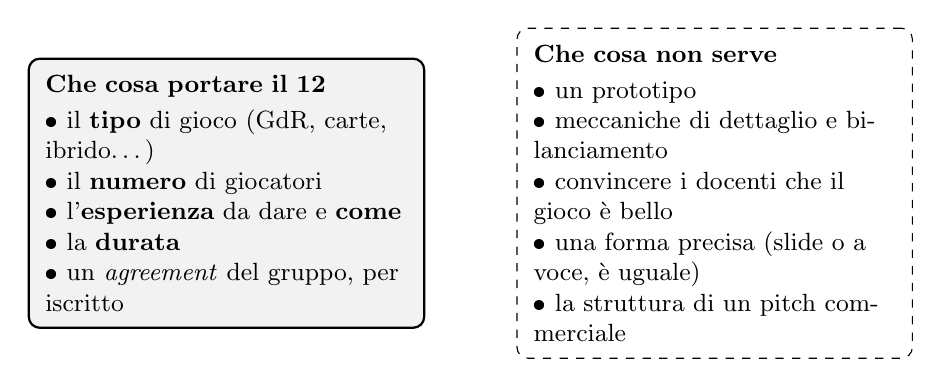
\begin{tikzpicture}[
    font=\small,
    si/.style={draw, thick, rounded corners, text width=4.6cm, align=left,
      fill=gray!10, inner sep=6pt},
    no/.style={draw, dashed, rounded corners, text width=4.6cm, align=left,
      fill=white, inner sep=6pt}
  ]
  \node[si] (a) at (0,0) {\textbf{Che cosa portare il 12}\\[2pt]
    \textbullet\ il \textbf{tipo} di gioco (GdR, carte, ibrido\ldots)\\
    \textbullet\ il \textbf{numero} di giocatori\\
    \textbullet\ l'\textbf{esperienza} da dare e \textbf{come}\\
    \textbullet\ la \textbf{durata}\\
    \textbullet\ un \emph{agreement} del gruppo, per iscritto};
  \node[no] (b) at (6.2,0) {\textbf{Che cosa non serve}\\[2pt]
    \textbullet\ un prototipo\\
    \textbullet\ meccaniche di dettaglio e bilanciamento\\
    \textbullet\ convincere i docenti che il gioco è bello\\
    \textbullet\ una forma precisa (slide o a voce, è uguale)\\
    \textbullet\ la struttura di un pitch commerciale};
\end{tikzpicture}
\caption{Il ``pitch'' del 12 ottobre come lo descrive Ruggero all'inizio della
lezione: un accordo sul \emph{che cosa}, non una vendita. Ricostruzione schematica.}
\label{a8:fig:pitch}
\end{figure}

% ---------------------------------------------------------------------
\section{Il programma: le mani nel motore}
\label{a8:sec:programma}

``Oggi, a livello logistico, vi dico cosa andiamo a fare''. Oggi è la lezione su
\textbf{Tabletop Simulator}: ``lavorare mani nel motore''. Il software va tenuto
aperto per tutta la lezione; chi non l'ha ancora installato lo installi subito (``non
è pesante, dovreste averlo pronto per tra 4 o 5 minuti''). Ci saranno domande e
momenti in cui chiedere di ``fermarmi a rispiegare una cosa'': ``fatelo, perché sono
qui apposta''.

\paragraph{Che cosa si dà per scontato.} Il software ``nasce per prototipare e
giocare'' giochi da tavolo. Ruggero dà per scontato che gli studenti l'abbiano già
usato \textbf{da giocatori} (\emph{user}, ``proprio di \emph{player}''), magari
giocando tra loro qualcosa che piace: serve ``il minimo necessario del sapersi
spostare all'interno del software'', cioè muovere la telecamera, cliccare sui menu,
sapere che cosa fanno i menu. Sono tutte cose che, come detto nel tutoraggio, ``il
tutorial di base vi spiega in 10 minuti''. Più complesso è \textbf{creare i moduli},
ed è quello che si fa oggi.

\paragraph{``Sì, ma con un asterisco''.} Tabletop Simulator è ``un software
gigantesco'' ed è impossibile coprirlo tutto in una lezione. Ruggero coprirà le
\textbf{basi} e lascerà l'ultima parte ai bisogni degli studenti: domande come ``si
può fare questa cosa qua su Tabletop Simulator?''. La risposta, ``come sempre, è quasi
sempre sì'': ``si può fare, con un asterisco: ma con un compromesso''. Il resto della
lezione spiegherà che cosa vuol dire.

Ruggero tiene il registro delle presenze in vista (``se per caso entra anche Giordano,
avvisatemi'') e condivide \textbf{tutto lo schermo}, non solo la finestra, perché
altrimenti i \emph{pop-up} del software non si vedono. Avverte che il programma, ``se
non l'avete mai aperto prima, può essere abbastanza ostile all'inizio''; ma alla fine
sarà chiaro perché è ``usatissimo nel settore'', e che ``non dovete stare 3000 ore per
saperlo usare bene''.

% ---------------------------------------------------------------------
\section{Avviare il software e creare una stanza}
\label{a8:sec:avvio}

Si lancia Tabletop Simulator da \textbf{Steam}. All'avvio il programma può proporre
un'opzione di lancio: giocare normalmente o avviare in modalità VR. Si sceglie il
gioco normale: ``è possibile usarlo con i set di realtà virtuale'', ma ``non siamo qua
per usare Tabletop in modalità VR''.

\paragraph{Il menu iniziale.} Nel menu si sente ``una musichetta fastidiosa'': si
toglie dall'ingranaggio, alla voce dei suoni, abbassando il volume del menu, ``così
magari riuscite anche a sentirmi senza impazzire''. L'icona della \textbf{lampadina}
apre il \textbf{tutorial} di base: ``io spero che voi l'abbiate già fatto. Se non
l'avete fatto, non ditemelo. Fatelo dopo la lezione senza dirmi niente, e io farò finta
che voi l'abbiate già fatto''. Poi ci sono le due voci grandi:
\begin{description}
  \item[Join] serve a unirsi a una partita che un'altra persona ha aperto; gli
        studenti dovrebbero già conoscerla, se hanno giocato con persone amiche.
  \item[Create] è quella che serve oggi: crea una partita \textbf{single player}, una
        \textbf{multiplayer} o una \textbf{hot seat}. L'\emph{hot seat} si ignora
        (``non la usa credo nessuno su questo pianeta, mai''). Il
        \emph{multiplayer} serve a creare partite con altri. Il \emph{single
        player} crea stanze in cui può entrare solo chi le crea, ed è quello che si
        usa per \textbf{costruire i moduli}.
\end{description}

\paragraph{I moduli si costruiscono in single player.} Ruggero è esplicito: ``non
create i moduli in multiplayer''. In multiplayer, del resto, solo l'\emph{host} può
crearli; ma soprattutto in single player è più comodo, perché ``la connessione
internet non vi chiederà costantemente il ping dei vostri compagni di stanza''.

All'apertura della stanza compare un \emph{pop-up} centrale, perché Tabletop
Simulator ``dà per scontato che noi vogliamo giocare qualcosa, non che vogliamo
creare un modulo''. Si chiude. Si resta con \textbf{un tavolo vuoto}, un panorama di
sfondo scelto a caso da un insieme predefinito e svariati menu. ``E a questo punto ci
dobbiamo chiedere: ok, benissimo. Cosa facciamo adesso?''.

% ---------------------------------------------------------------------
\section{``Un gioco da tavolo è un gioco su un tavolo''}
\label{a8:sec:simulatore}

Si parte ``dalle basi, proprio basi, basi''. Ruggero avverte che la lezione sarà
``piena di banalità'': frasi che suonano banalissime, ma che nell'ottica di Tabletop
Simulator ``non sono così banali''. E ripete un'informazione che era già stata messa
lì, ``nascosta, per fare \emph{foreshadowing}'', e che ripeterà ``fino allo
sfinimento'':

\begin{quote}
\textbf{Tabletop Simulator non è un software per fare videogiochi.} Non uscirete da qua
con il videogioco del vostro gioco da tavolo. Non vi serve a quello. Tabletop
Simulator, come il nome fa intuire, è un simulatore di giochi \emph{tabletop}. Vuol
dire che tutto quello che vedrete qua è \textbf{simulato fisicamente}: con un peso,
con una massa, con uno spazio, con delle collisioni.
\end{quote}

È il principio che regge tutta la lezione, e Ruggero lo riprenderà ogni volta che un
componente si comporta in modo inatteso: un mazzo che sul bordo del tavolo resta
inclinato, un cubetto che rotola giù dalla cornice di una plancia, una carta bucata
che però collide come se fosse intera. ``Questo è un simulatore di spazio fisico.
Spero che, se c'è una cosa che vi entra da oggi, è questa''. La conseguenza pratica:
i componenti di un modulo \textbf{vanno trattati come componenti fisici}, con le
stesse attenzioni che si avrebbero su un tavolo vero.

\paragraph{Approfondimento: il prototipo come simulazione.} La distinzione di Ruggero
tra \emph{simulatore} e \emph{motore} è la stessa che separa un prototipo di un gioco
da tavolo dalla sua versione digitale. Un adattamento digitale \emph{applica} le
regole al posto dei giocatori; un simulatore fisico, invece, lascia le regole ai
giocatori, come il tavolo vero, e si limita a riprodurre gli oggetti. È proprio questo
che lo rende adatto al \emph{playtest}: Schell, in \emph{The Art of Game Design},
insiste che ogni prototipo deve rispondere a una domanda precisa, e che la sua
fedeltà va scelta in funzione di quella domanda. Un prototipo su TTS risponde bene
alle domande su regole, spazio e flusso del turno, perché i giocatori devono ancora
eseguire tutto a mano, come farebbero con la scatola; risponde male, per costruzione,
alle domande che riguardano la manualità e il tatto. Il divieto degli \emph{script}
che Ruggero darà a fine lezione (sezione~\ref{a8:sec:script}) nasce dalla stessa
logica.

% ---------------------------------------------------------------------
\section{Il tavolo e la table presence}
\label{a8:sec:tavoli}

Nel menu in alto c'è la voce \textbf{Oggetti}, con quattro sottomenu:
\textbf{componenti}, \textbf{tavoli}, \textbf{background} e \textbf{oggetti
salvati}. Si parte dal tavolo.

\paragraph{Non tutti i giochi stanno su tutti i tavoli.} Nella vita reale, ``nella vita
di tutti i giorni, fisicamente'', alcuni giochi da tavolo su alcuni tavoli non si
possono giocare. Su un tavolino da caffè ``non ci sta probabilmente tutto
\emph{Twilight Imperium}''; sui tavolini del treno non ci si gioca un
\emph{eurogame}, ``perché il tavolo è più piccolo''. Allo stesso modo, quando si pensa
alla \textbf{table presence} del proprio gioco, cioè allo \textbf{spazio che occupa sul
tavolo}, la scelta non è casuale: non lo è nel mondo reale e non lo è su Tabletop
Simulator, perché lo spazio fisico è limitato: ``le cose che non sono sul tavolo
cadono dal tavolo''.

Il software offre \textbf{dieci tavoli}. Ruggero li mostra uno per uno
(tabella~\ref{a8:tab:tavoli}), guardando ogni volta due cose: quanti \textbf{posti}
ha e com'è fatto il \textbf{bordo}.

\paragraph{Le mani sono i posti a sedere.} Per contare i posti si usa, nel menu a
sinistra, la voce \textbf{Zone}, sottovoce \textbf{Hands}: mostra le \textbf{mani} di
carte, cioè le persone al tavolo. ``La \emph{hand} è in tutto e per tutto quanti
posti a sedere ci sono''. Se il tavolo ha quattro mani, ``questo gioco non può tenere
fisicamente più di quattro persone''; se si progetta un gioco da 6--8 persone, quel
tavolo ``già non va bene''.

\paragraph{Perché guardare i bordi.} ``So che vi sembra apparentemente inutile questa
informazione'', ma sopra il tavolo ci saranno dei componenti, e i componenti sono
oggetti fisici. Un bordo tridimensionale impedisce di tenere a bordo tavolo, ``belle
piatte, tranquille'', le plance dei giocatori; un rilievo al centro impedisce di
appoggiarvi piatta una plancia o un tabellone, perché ``questa salita qua è una
salita fisica che andrà a impattare i vostri componenti''.

\begin{table}[htbp]
\centering
\small
\begin{tabular}{@{}p{2.7cm}p{1.2cm}p{8.6cm}@{}}
\toprule
\textbf{Tavolo} & \textbf{Posti} & \textbf{Che cosa ne dice Ruggero} \\
\midrule
Square & 4 & piccolo, ``piccolino''; quattro persone ``strettine'' \\
Hexagon & 6 & un posto per lato, forma ``bizzarra''; \textbf{bordi
tridimensionali}: niente plance piatte a bordo tavolo \\
Octagon & 8 & come l'esagonale, con otto posti \\
Round & 8 & bordi molto meno marcati, ma al centro un \textbf{cerchio di vetro in
rilievo}: niente tabellone piatto al centro \\
Poker & -- & ``non vi servirà, a meno che non dobbiate fare poker'' \\
Rectangle & 8 & ``belli larghi''; bordi scanalati, ma superficie ampia: va bene per
``la maggior parte dei giochi pubblicati oggi'' \\
Round Glass & 8 & rotondo, grande, di vetro semitrasparente, con le gambe visibili
sotto, ``in stile Escher'': ``il tavolo peggiore di tutti. Non usatelo mai'' \\
Custom Rectangle & 8 & accetta un'immagine come superficie; il più grande; non se ne
sceglie la dimensione; l'immagine viene \textbf{stirata} \\
Custom Square & 8 & accetta un'immagine; gambe metalliche riflettenti; ``sembra
piccolo, ma è gigante''; nessun bordo strano \\
None & -- & nessun tavolo: i componenti ``cadono all'infinito in questo pozzo senza
fondo''. È l'opzione preferita di Ruggero, per un motivo che spiegherà dopo
(sezione~\ref{a8:sec:moduli}) \\
\bottomrule
\end{tabular}
\caption{I dieci tavoli di Tabletop Simulator come li presenta Ruggero. I nomi sono
quelli dell'interfaccia; i posti sono le \emph{hands} visibili nella voce
\emph{Zone}\protect\footnotemark.}
\label{a8:tab:tavoli}
\end{table}
\footnotetext{Per il tavolo da poker e per quello di vetro la trascrizione non riporta
il numero di posti (per il secondo dice solo ``per otto persone''). Il nome
``Round Glass'' per il tavolo di vetro è quello dell'interfaccia, che Ruggero non
pronuncia: lo descrive soltanto.}

\paragraph{Perché il software è fatto così.} Davanti al tavolo rotondo con il rilievo
al centro, la domanda viene da sé: perché qualcuno l'ha fatto? La risposta di Ruggero,
che tornerà molte volte nella lezione, è un misto di esasperazione e di affetto:
``perché sono pazzi'', ``è un miracolo che esista''. Chi ha creato il software ``non
sapeva cosa stava facendo''; oggi ci si ritrovano ``delle scelte vestigiali di gente
fulminata di anni fa che, contro la loro volontà, hanno purtroppo creato il software
di riferimento del settore, che è quello che tutti usano adesso''. E con queste scelte
``dobbiamo venire a patti''.

\paragraph{La scelta della lezione.} Per il prototipo dimostrativo Ruggero sceglie il
\textbf{tavolo quadrato custom} con una texture di legno: ``abbiamo un gioco piccolo,
magari un \emph{fillerino} per quattro persone, perfetto''. Sul tavolo senza tavolo
(\emph{None}) promette di tornare: ``ve lo spiego dopo, perché potrebbe essere
interessante''.

% ---------------------------------------------------------------------
\section{Caricare un'immagine: file locale e cloud}
\label{a8:sec:caricare}

Il tavolo \emph{Custom Rectangle}, appena selezionato, apre un \emph{pop-up} che chiede
un'\textbf{immagine}. È il primo incontro con una procedura che si ripeterà per quasi
ogni componente custom, e Ruggero ne fissa subito le due regole.

\paragraph{Regola 1: mai un URL, sempre un file.} Su Tabletop Simulator un oggetto
custom si può creare in due modi: dandogli l'\textbf{URL} di un'immagine online o
caricando un'immagine dal proprio computer (\textbf{Browse Local Files}). ``Il mio
consiglio personale è: non dategli mai un URL immagine'', perché se qualcuno, per
qualunque motivo, toglie quell'immagine dal suo indirizzo, ``il vostro modulo crolla''.
Se online c'è un'immagine che piace, la si \textbf{scarica} e la si ricarica dalla
propria cartella.

\paragraph{Regola 2: mai in locale, sempre in cloud.} Quando si carica un file, il
software chiede se caricarlo \textbf{in cloud} o \textbf{in locale}. ``Non caricate mai
niente del vostro modulo in locale'': un modulo con immagini locali non si può usare
in multiplayer, funziona solo sul proprio computer, e questo ``sconfigge un po'
l'obiettivo'' di farlo vedere, per esempio, a un \emph{publisher} esterno. Si carica
quindi in cloud, gli si può dare un nome, si aspetta che ``finisca di circolare questo
cerchiettino'' e si fa \textbf{Import}.

\paragraph{Le proporzioni.} Ruggero carica prima una texture di legno, poi un
tabellone più elaborato\footnote{La trascrizione descrive l'immagine come ``le
influenze moderne nella scena del Nord di Clarp'': con ogni probabilità è la
copertina o una pagina di un lavoro sul LARP nordico, usata a caso come esempio; il
contenuto dell'immagine non ha importanza.}: sul tavolo si può avere un tabellone,
uno schema, delle zone, ``già qualcosa di meccanico''. Ma la dimensione del tavolo non
si può definire: è il tavolo più grande che c'è, e l'immagine vi si adatta. Con una
texture verticale (una ``A'' arancione), il software ``la streccia come se non ci fosse
un domani'', e in più crea una luce arancione in faccia ``che sembra uscita da un film
sci-fi''. Quindi: \textbf{occhio alle proporzioni} delle immagini. Di solito il tavolo
si usa \textbf{con una texture}, e i tabelloni si mettono \textbf{a parte}, senza
caricarli direttamente sul tavolo, perché il tavolo li distorce.

% ---------------------------------------------------------------------
\section{Lo sfondo cambia la luce}
\label{a8:sec:sfondi}

Scelto il tavolo, Ruggero fa notare che la scena è buia: il suo sfondo è ``sera al
crepuscolo'', in mezzo a un prato, ``con tutto il problema di illuminazione che ne
deriva''. Il motivo è che Tabletop Simulator simula la \emph{skybox}, l'ambiente
attorno al tavolo. Dalla voce \textbf{Background} si sceglie lo sfondo: ``in questo
momento abbiamo il \emph{sunset}'', poi c'è il \emph{tunnel}, e così via.

Cambiando sfondo, Ruggero chiede di guardare il tavolo: che cosa succede? Uno studente
risponde: cambia il riflesso. Sì, e cambiano anche il livello di illuminazione e
l'angolazione. Non solo sulle gambe metalliche, che riflettono, ma anche sulla texture
di legno, che non è metallica: ingrandita, mostra colori ``più freddi, più caldi in base
a dove sono''. La luce, in Tabletop Simulator, arriva \textbf{da tre direzioni}:
\textbf{dall'alto}, \textbf{dall'orizzonte} e come \textbf{riflesso dal basso}. ``Stiamo
nel tecnico, mi rendo conto''; per ora il prato va benissimo. La questione tornerà con
il PDF, quando si vedrà che lo sfondo può rendere illeggibile un componente
(sezione~\ref{a8:sec:luce}).

% ---------------------------------------------------------------------
\section{I componenti: importare o creare?}
\label{a8:sec:componenti}

Abbiamo il tavolo, abbiamo lo sfondo, ``fantastico''. Ma mancano i componenti per
giocare. ``Vi sorprenderà sapere'' che dalla voce \textbf{Oggetti}, sottovoce
\textbf{Componenti}, si possono mettere dei componenti sul tavolo. I componenti sono
divisi in \textbf{16 categorie}, alcune più personalizzabili di altre. E l'approccio da
avere con questo software, per ogni pezzo del proprio gioco, è una domanda in due
tempi:

\begin{quote}
Devo importare un componente nel mio gioco? Ho qualcosa che mi può servire
\textbf{che già esiste}? O devo \textbf{crearlo da zero}?
\end{quote}

Ruggero passa quindi prima in rassegna i componenti ``più o meno standardizzati'' e il
modo di adattarli, e solo alla fine i componenti \emph{ad hoc}, i \textbf{custom}.

\subsection{Blocchi e cubetti}
\label{a8:sec:cubetti}

Nella categoria \textbf{Blocchi} ci sono un quadrato, un rettangolo e un triangolo; si
trascinano sul tavolo e si nota che sono \textbf{3D}. Rettangoli e triangoli per ora
non servono: si tengono i \textbf{cubetti}, una risorsa ``usatissima'' nei giochi da
tavolo. Ruggero chiede un esempio di gioco con i cubetti: gli studenti citano
\emph{Terraforming Mars} e \emph{Azul}\footnote{``Asol'' e ``terraform in Mars'' (poi
``terraform in Mark'') nella trascrizione. Ruggero aggiunge che in \emph{Azul} ci sono
``i cubetti neri per il contafonti'': il dettaglio non è ricostruibile con certezza
dalla trascrizione.}.

\paragraph{Ricolorare.} Il problema è che il cubetto è rosso, e nei giochi citati i
cubetti hanno altri colori. ``Ci può andare bene come forma, ma non come colore''. Per
ricolorarlo: \textbf{tasto destro}, \textbf{Color Tint}, e si sceglie il colore con la
classica barra di tonalità e saturazione, ``inclusa la semitrasparenza'': la barra in
fondo regola la trasparenza, e un cubetto blu con la barra abbassata diventa
semitrasparente. Un cubetto ``di grano'' si fa giallo, e così via.

\paragraph{Copiare.} Mentre si creano i moduli si possono usare \texttt{Ctrl+C} e
\texttt{Ctrl+V}: ``io posso copiarmi questi cubetti quanti ne voglio''.

\paragraph{Ridimensionare.} Un componente si può ingrandire o rimpicciolire dalla
tastiera, con i tasti \texttt{+} e \texttt{-}: per esempio un cubo più grande degli
altri, che valga tre o cinque risorse.

\subsection{Le dimensioni reali}
\label{a8:sec:misurare}

Il ridimensionamento serve per tutti i componenti, e qui Ruggero chiede di
``prepararsi psicologicamente'': quando si fanno moduli su Tabletop Simulator,
\textbf{è buona pratica mantenere le dimensioni e le proporzioni reali dei
componenti}. Ma come si sa quanto è grande un cubo? ``Può essere 10 cm, come 150, che
ne sappiamo''.

\paragraph{Lo strumento Linea.} Nel menu a sinistra c'è lo strumento \textbf{Linea}
(il righello). Nelle sue impostazioni si sceglie l'\textbf{unità}: Ruggero consiglia i
\textbf{centimetri} e la modalità 2D\footnote{La trascrizione rende le impostazioni
consigliate come ``2D free edge no log''; Ruggero dice di non volerle spiegare ``per
limiti di tempo'' e che ``centimetri, 2D'' è quello che serve. La forma esatta delle
altre voci non è ricostruibile dalla trascrizione.}. Con lo strumento si tira una
linea e il software scrive la misura sul bordo: il lato del cubo è ``più o meno 8
cm''.

\paragraph{Misurare dall'alto.} Per misurare con precisione si cambia prospettiva con
il tasto \texttt{P}, passando alla vista \textbf{dall'alto} (\emph{top-down}): senza
il problema del 3D si misura ``da un angolo all'altro''. Il lato risulta di 7 cm.
Se il cubetto dev'essere di 20 mm, lo si ridimensiona con \texttt{+} e \texttt{-}
finché la misura non è ``più o meno 2 cm''.

\paragraph{Una domanda di chiarimento.} Uno studente non ha capito: il cubo è stato
ridimensionato con la linea? No: il cubo si ridimensiona \textbf{con i tasti più e
meno}; la linea \textbf{misura} soltanto. Il tasto \texttt{Tab}, premuto una volta,
mette le freccette per indicare le cose; \textbf{tenuto premuto}, mostra la linea di
misura. Un'altra studentessa non ha capito come cambiare prospettiva: tasto \texttt{P},
``di prospettiva'', che passa tra prima persona, terza persona e vista dall'alto. Sono
cose che il tutorial dovrebbe aver già insegnato; in ogni caso, con il tasto
\texttt{Esc} si apre l'\textbf{Help}, con tutte le scorciatoie del software. Anche
spostare più componenti insieme e interagire con i componenti sono cose del tutorial.

\begin{figure}[htbp]
\centering
\begin{tikzpicture}[
    font=\small,
    passo/.style={draw, thick, rounded corners, text width=2.6cm, align=center,
      minimum height=1.3cm, fill=gray!10},
    freccia/.style={-{Stealth[length=2.5mm]}, thick}
  ]
  \node[passo] (a) at (0,0) {Linea: unità in \textbf{cm}, modalità \textbf{2D}};
  \node[passo] (b) at (3.3,0) {\texttt{P}: vista \textbf{dall'alto}};
  \node[passo] (c) at (6.6,0) {\texttt{Tab} tenuto premuto: \textbf{misura}};
  \node[passo] (d) at (9.9,0) {\texttt{+} / \texttt{-}: \textbf{scala} fino alla misura reale};
  \draw[freccia] (a) -- (b);
  \draw[freccia] (b) -- (c);
  \draw[freccia] (c) -- (d);
  \draw[freccia, dashed] (d.south) to[bend left=25] node[below, font=\footnotesize]
    {si rimisura finché non torna} (c.south);
\end{tikzpicture}
\caption{Come portare un componente alle sue dimensioni reali, secondo la procedura
mostrata da Ruggero: nell'esempio, un cubetto da 7 cm ridotto a 2 cm.}
\label{a8:fig:misurare}
\end{figure}

% ---------------------------------------------------------------------
\section{Le plance}
\label{a8:sec:plance}

La categoria \textbf{Board} contiene le \textbf{plance}: backgammon, scacchi o dama,
un'altra versione della scacchiera, dama cinese, Go, Reversi. ``La domanda però è:
perché ci sono?''. Il proprio gioco sarà sicuramente diverso da questi: quello che
serve, di solito, è la \textbf{Custom Board}, che chiede, ``indovinate un po''',
un'immagine, come il tavolo custom.

\paragraph{Bloccare la plancia.} La plancia si può spostare; con il tasto \texttt{L},
di \emph{lock}, la si \textbf{blocca}, in modo che cliccandoci sopra, anche per
sbaglio, non si sposti più. ``Questa è una buona pratica, perché noi non vogliamo che
qualcuno sposti il tabellone con tutte le cose sopra''.

\paragraph{La plancia si adatta all'immagine.} Uno studente nota che la plancia ha
cambiato dimensione da sola. Esatto: \textbf{al contrario del tavolo}, che adatta
l'immagine alla cornice (stirandola), \textbf{la board adatta la cornice
all'immagine}. Un'immagine alta dà una plancia stretta e alta; cambiandola (tasto
destro, \textbf{Custom}) con la texture del tavolo, la plancia si allunga dall'altro
lato. Ne segue una regola per i tabelloni: importarli \textbf{nelle proporzioni che
devono avere nella realtà}.

\paragraph{Il problema della cornice.} ``Ma adesso ti faccio vedere un'altra cosa''.
La plancia custom ha un \textbf{bordo di legno} in rilievo, ``nello stile delle vecchie
scacchiere''. E siccome i componenti sono 3D, un cubo appoggiato sul bordo
\textbf{rotola giù}. ``Quanti board game recenti avete visto con le plance che hanno la
cornice in legno alta due centimetri?''. Nessuno, risponde uno studente; ``forse una
versione super antica degli scacchi di mio nonno''. ``Esatto, perché è una roba da
fuori di testa'': nessuno mette una cornice di legno su un tabellone che costa 200
euro. La cornice non si può togliere. La soluzione arriverà più avanti
(sezione~\ref{a8:sec:tabellone}); per ora: ``tenetevi in background l'informazione''.

% ---------------------------------------------------------------------
\section{Le carte standard}
\label{a8:sec:carte-std}

La categoria \textbf{Carte} contiene: uno \emph{standard deck}, un \emph{custom deck},
una \emph{custom card}, una carta a caso (``randomicamente ci pesca una carta a
caso''), un \textbf{Jolly} (perché il mazzo standard è ``il classico deck da poker
normale di 52 carte'' e non ha i Jolly) e alcuni mazzi creati dagli autori di Tabletop
Simulator per un loro gioco, ``che non servono a niente di niente'': ``li lanciamo nel
sole''.

Come si interagisce con un mazzo (spostarlo, pescare, rivelare, pescare nella propria
mano) lo insegna il tutorial. Quello che importa sapere è che il mazzo \textbf{ha una
proprietà fisica}: la carta singola è più leggera del resto, il mazzo è
tridimensionale, e un mazzo appoggiato sul bordo del tavolo resta \textbf{inclinato},
tanto che si può vedere che cosa c'è sotto. ``Questo è un simulatore di spazio fisico.
Spero che, se c'è una cosa che vi entra da oggi, è questa''. I componenti ``vanno
trattati come se fossero componenti fisici''.

E se il gioco usa un mazzo di carte evento personalizzate? ``Ve lo spiego dopo'': prima
i componenti standard e come adattarli, ``e poi passiamo per ultimo ai componenti
\emph{ad hoc} vostri'' (sezione~\ref{a8:sec:mazzo}).

% ---------------------------------------------------------------------
\section{Dama, scacchi, dadi e figurine}
\label{a8:sec:dadi}

\paragraph{Dama e scacchi.} La quarta categoria sono i pezzi della \textbf{dama}, ``e
qui davvero abbiamo la follia di Tabletop Simulator'': c'è di nuovo la plancia,
identica a quella della categoria precedente, presente quindi in due categorie. Negli
\textbf{scacchi} ci sono pezzi metallici o di legno; ``se volete dei riflessi
ambientali, quelli di metallo sono perfetti''. Ma la domanda è sempre: servono?
Trattandosi di prototipi, se serve un pedone, ``nessuno si scandalizza se prendete un
pedoncino così e magari lo colorate, che so, rosso''.

\paragraph{I dadi.} Nella categoria \textbf{Dadi} ci sono dadi metallici e di plastica,
già colorati: d4, d6, d8, d10, d12 e d20, più altre versioni (per esempio d6 colorati
con gli angoli arrotondati). Si possono ricolorare e ingrandire: ``mi servono da 20,
ma blu''; lo si ricolora, lo si fa più grosso degli altri, e si tira come gli altri.
Ma attenzione: \textbf{ricolorare un componente non colora tutto}. Un dado bianco
colorato di giallo mantiene i \textbf{pallini} neri; un dado metallizzato colorato di
giallo ha i pallini bianchi, ed è \textbf{illeggibile}; un dado colorato di nero ``fa
schifo'', uno colorato di bianco è ``completamente illeggibile''. Quindi: attenzione a
quali componenti si scelgono come base.

\paragraph{Le figurine.} Nella categoria \textbf{Figurine} ci sono gli \emph{standee}
(le sagome in piedi) e le figurine metalliche, ``i classici omini di piombo'', che non
servono. Serve il \textbf{custom standee}, che chiede un'immagine di \textbf{fronte} e
una di \textbf{retro}. Ruggero vi mette la sua ``A'' davanti e dietro, ``ed ecco il
nostro standee''. Può essere un personaggio anche con la trasparenza: un PNG ritagliato
mantiene lo sfondo trasparente. Per avere un'immagine più grande mantenendo la base
piccola si usa il fattore di \textbf{scala}: con 2, l'immagine raddoppia e la base
resta piccola. ``Mi rendo conto che può essere estremamente noioso per ora questo
software''; tra poco arrivano ``le cose custom per davvero''.

% ---------------------------------------------------------------------
\section{Go, biglie, miscellanea}
\label{a8:sec:misc}

Ruggero passa ``velocissimamente'' sul resto.

\paragraph{Le pedine del Go.} Le pietre del Go ``possono essere come risorse'': si
vogliono risorse che siano sassolini, anziché cubetti? Benissimo. Colorate di azzurro
e rese semitrasparenti, diventano ``delle gocce d'acqua''.

\paragraph{Le biglie e i giochi di destrezza.} Le \textbf{biglie} sono biglie,
``letteralmente, con tutta la fisica che ne comporta'': su una superficie piana
continuano a rotolare. A che cosa servono? Ai \textbf{dexterity game}, i giochi di
destrezza, che si possono fare anche qui. La dimostrazione: Ruggero prende un
componente, lo mette sul tavolo e lo blocca; poi usa lo strumento \textbf{Flick} (il
``colpetto'' con il dito) sulla biglia, che va a sbatterci contro. ``Voilà! È un
simulatore fisico questo software''.

\paragraph{La miscellanea.} ``Dentro la miscellanea abbiamo tante cose bizzarre''.
\begin{itemize}
  \item Una \textbf{ciotola}: come componente non serve, ma bloccata sul tavolo e
        riempita di cubetti dà ``improvvisamente una \emph{table presence}
        diversa''.
  \item Una \textbf{moneta}, che lanciata dice testa o croce.
  \item Le pedine del \textbf{Reversi}, a due facce, una bianca e una nera: un
        \emph{token} a due lati già pronto.
  \item Pezzi del \textbf{domino}, tessere del \textbf{Mahjong}\footnote{``Testa del
        Maggiog'' nella trascrizione.}, altri dischetti, tutti ricolorabili, da
        usare come risorse.
  \item Un insieme di componenti dei designer del software\footnote{La trascrizione
        lo chiama ``P-Spec''; il nome della categoria non è ricostruibile con
        certezza.}: ``se vi servono, bene; se no, il mio sospetto è che non vi
        serviranno mai''.
  \item I \textbf{Player Pawn}, i classici pedoni di plastica, in \textbf{nove
        colori}. Perché nove versioni, se si possono ricolorare? ``Perché sono pazzi, i
        designer: non ci hanno pensato''. Ricolorateli come volete.
\end{itemize}

\paragraph{I colori dei giocatori.} C'è però una ragione per ricolorare con criterio.
Nel selettore dei colori, la colonna a destra contiene esattamente i \textbf{colori dei
giocatori}, cioè i colori delle mani attorno al tavolo\footnote{Ruggero dice prima
``questi 16 colori'' e poi ``esattamente i 12 colori player''; la trascrizione non
permette di stabilire quale dei due numeri sia quello inteso.}. Se si vuole un codice
colore preciso, legato al giocatore, si sceglie da lì: ``fammelo di questo arancione''
dà esattamente l'arancione del giocatore arancione.

\paragraph{Fiches e kit da GdR.} Poi le \textbf{fiches} da poker, ``classiche fiches
da casinò''; e il \textbf{RPG Kit}: miniature su miniature da \emph{dungeon crawler},
maghi, guerrieri, mostri, creature. ``Si muovono da sole queste'' (sono animate), ``un
po' anni Duemila, ma oh: per un prototipo su TTS, chi se ne frega?''.

\paragraph{Le cose ``fulminate''.} Infine la categoria preferita di Ruggero: ``le cose
così fulminate che mi fanno chiedere: ma perché, perché, perché hanno messo queste
cose qua? Non avremo mai una risposta''.
\begin{itemize}
  \item Una \textbf{Notecard}: un foglietto su cui si scrive con il tasto destro,
        compilando \textbf{nome} (il titolo) e \textbf{descrizione}. Si chiamano
        \textbf{index card}, ``usatissime per i giochi di ruolo in ambito americano,
        il \emph{tabletop} RPG specialmente''. Una studentessa si è persa: come si
        scrive? Tasto destro, e in fondo ci sono i due campi, nome e descrizione; si
        può andare a capo e mettere più righe; il testo ``non è in tempo reale'', si
        aggiorna solo quando si esce dal menu.
  \item Un \textbf{lettore MP3}: ``che devo dirvi? C'è un lettore MP3. Se volete
        giocare con la musica, ce l'abbiamo''. (Ruggero verifica che la classe senta
        l'audio del suo computer: ``vi voglio far soffrire per davvero''.)
  \item Un \textbf{contatore}, che si può far salire, scendere, azzerare, o in cui si
        scrivono direttamente i numeri.
  \item Un \textbf{tablet}, ``letteralmente un tablet'': ci si può aprire YouTube e
        guardare video. ``È un tablet, ragà, è un tablet. Non so che dirvi''.
  \item Una \textbf{sveglia} e una \textbf{calcolatrice}.
\end{itemize}

% ---------------------------------------------------------------------
\section{I sacchetti}
\label{a8:sec:sacchetti}

Nella miscellanea ci sono finalmente ``le due cose che ci servono per davvero'': il
\textbf{sacchetto infinito} e il \textbf{sacchetto}.

\paragraph{Il sacchetto infinito.} Parte vuoto e rende infinito qualunque cosa gli si
metta dentro: con un dado blu diventa un sacchetto infinito di dadi blu. Si può
ricolorare e si può azzerare (tasto destro, \textbf{Reset}) per farne, per esempio, un
sacchetto di dadi rossi. Ma Ruggero fa una richiesta precisa: \textbf{nei moduli per
questo corso non si usa il sacchetto infinito}, perché ``a livello produttivo io vi
chiederò quanti componenti avete, e infiniti non è un numero che è possibile stampare
nella realtà''. Per comodità è utilissimo, ``ma non è questo il momento''.

\paragraph{Il sacchetto normale.} Parte vuoto (passandoci sopra con il mouse si legge
zero) e ci si mette dentro qualunque cosa. Ruggero colora tre cubetti di giallo, rosso
e blu e li mette nel sacchetto; poi, con il tasto destro, decide \textbf{in che ordine}
il sacchetto restituisce gli oggetti (figura~\ref{a8:fig:sacchetto}):
\begin{description}
  \item[LIFO] (\emph{last in, first out}): l'ultimo oggetto messo è il primo a
        uscire. Messi blu, rosso, giallo, escono giallo, rosso, blu.
  \item[FIFO] (\emph{first in, first out}): il primo messo è il primo a uscire.
        Messi blu, rosso, giallo, escono blu, rosso, giallo.
  \item[Random]: ``è random''.
\end{description}
``Chiaramente non siamo persone fulminate'': un sacchetto, nella realtà, si comporta in
modo casuale, e quindi si mette \textbf{Random}. Nella prova, blu, rosso, giallo escono
giallo, rosso, blu.

\paragraph{Guardare dentro.} Per vedere che cosa c'è nel sacchetto: tasto destro,
\textbf{Search}. La stessa funzione si usa sui \textbf{mazzi}, per vedere le carte
rimaste.

\begin{figure}[htbp]
\centering
\begin{tikzpicture}[
    font=\small,
    cubo/.style={draw, minimum size=0.55cm, inner sep=0pt},
    etich/.style={font=\small\bfseries, anchor=east},
    freccia/.style={-{Stealth[length=2mm]}, thick}
  ]
  % ingresso
  \node[font=\footnotesize] at (0.9,1.9) {si inserisce};
  \node[cubo, fill=blue!40] at (0,1.3) {B};
  \node[cubo, fill=red!40] at (0.9,1.3) {R};
  \node[cubo, fill=yellow!50] at (1.8,1.3) {G};
  \draw[freccia] (2.3,1.3) -- (3.3,1.3);
  \node[draw, thick, rounded corners=6pt, minimum width=1.5cm, minimum height=1.2cm,
    align=center, font=\footnotesize] at (4.2,1.3) {sacchetto};
  % uscite
  \node[etich] at (7.2,2.2) {LIFO};
  \node[cubo, fill=yellow!50] at (7.7,2.2) {G};
  \node[cubo, fill=red!40] at (8.4,2.2) {R};
  \node[cubo, fill=blue!40] at (9.1,2.2) {B};
  \node[etich] at (7.2,1.3) {FIFO};
  \node[cubo, fill=blue!40] at (7.7,1.3) {B};
  \node[cubo, fill=red!40] at (8.4,1.3) {R};
  \node[cubo, fill=yellow!50] at (9.1,1.3) {G};
  \node[etich] at (7.2,0.4) {Random};
  \node[cubo] at (7.7,0.4) {?};
  \node[cubo] at (8.4,0.4) {?};
  \node[cubo] at (9.1,0.4) {?};
  \draw[freccia] (5.1,1.3) -- (5.5,2.2);
  \draw[freccia] (5.1,1.3) -- (5.5,1.3);
  \draw[freccia] (5.1,1.3) -- (5.5,0.4);
  \node[font=\footnotesize] at (8.4,2.8) {ordine di uscita};
\end{tikzpicture}
\caption{Le tre modalità del sacchetto, con l'esempio di Ruggero: tre cubetti
inseriti nell'ordine blu, rosso, giallo (B, R, G). Per un gioco da tavolo si usa
\emph{Random}, che è il comportamento di un sacchetto reale.}
\label{a8:fig:sacchetto}
\end{figure}

\paragraph{Approfondimento: il prototipo e la produzione.} La richiesta di non usare il
sacchetto infinito anticipa un tema che il corso affronterà con la lezione sulla
produzione: un gioco analogico è anche una \textbf{distinta dei componenti}, e ogni
componente ha un costo. Un modulo che usa scorte infinite nasconde al designer la
domanda ``quanti me ne servono davvero?'', che in un gioco stampato ha sempre una
risposta. Lo stesso vale per i cubetti copiati a volontà con \texttt{Ctrl+V}: comodi
per costruire, ma da contare prima di consegnare.

% ---------------------------------------------------------------------
\section{I componenti custom}
\label{a8:sec:custom}

``Allora, adesso arriviamo alla parte più incubo di tutte, che è la parte custom''. La
categoria \textbf{Custom} raduna tutte le opzioni personalizzabili, comprese quelle già
viste (la plancia, le figurine). Sono dieci (tabella~\ref{a8:tab:custom}).

\begin{table}[htbp]
\centering
\small
\begin{tabular}{@{}p{2.6cm}p{10.0cm}@{}}
\toprule
\textbf{Componente} & \textbf{A che cosa serve e che cosa ne dice Ruggero} \\
\midrule
Custom Board & una plancia da un'immagine; la cornice si adatta all'immagine, ma ha
il bordo di legno (sezione~\ref{a8:sec:plance}) \\
Custom Figurine & lo \emph{standee} con fronte e retro (sezione~\ref{a8:sec:dadi}) \\
Custom PDF & il \textbf{regolamento} del gioco, consultabile sul tavolo \\
Custom Token & un gettone con \textbf{forma libera} (gestisce la trasparenza e la
collisione), colorabile, impilabile; il retro è specchiato \\
Custom Tile & una tessera di \textbf{forma regolare} (quadrata, esagonale, circolare,
arrotondata) con fronte e retro corretti \\
Custom Deck & un \textbf{mazzo} di carte da una griglia di immagini: ``la parte più
difficile di tutte'' \\
Custom Card & una carta singola, fronte e retro \\
Custom Dice & un dado con le facce personalizzate, da un \emph{template} \\
Custom Model & un modello 3D (mesh, texture, collider): non si vede a lezione \\
Custom AssetBundle & pacchetti di modelli 3D, per esempio miniature: non si vede a
lezione \\
\bottomrule
\end{tabular}
\caption{I dieci componenti della categoria \emph{Custom}, come Ruggero li elenca
(``board, tile, token, figurine, deck, card, dice, model, asset bundle, PDF''). Modelli
3D e asset bundle in fase di prototipo sono fortemente sconsigliati.}
\label{a8:tab:custom}
\end{table}

% ---------------------------------------------------------------------
\section{Il PDF del regolamento e la luce}
\label{a8:sec:luce}

\paragraph{Caricare un PDF.} Il \textbf{Custom PDF} chiede di caricare un PDF. Ruggero
ne carica uno a caso, ``così a caso'': un PDF sul \emph{framework} DPE\footnote{``DPA
Framework'' nella trascrizione; con ogni probabilità il materiale sul framework DPE
(\emph{Design, Play, Experience}) visto nelle lezioni precedenti.}. ``Sempre
aspettare che finisca questa rondella blu, se no TTS impazzisce''. Il PDF appare sul
tavolo: è \textbf{molto piccolo} ed è \textbf{molto bianco}, quasi illeggibile, perché
l'illuminazione dello sfondo ``fa schifo''. Ed ecco il punto chiave sugli sfondi,
``lasciato in sospeso'' fino ad ora: cambiando lo sfondo cambia tutto. Ma magari non si
vuole giocare ``con le vibes di un pub di fumatori incalliti''.

\paragraph{Uno sfondo da un pixel.} Nel menu degli sfondi c'è un'opzione che Ruggero
aveva taciuto apposta: \textbf{Custom}, che permette di scegliere uno sfondo proprio.
Tabletop Simulator usa per gli sfondi panorami HDRI da $4000\times2000$ pixel, in un
formato specifico; ``ma non ce ne frega niente, perché in realtà noi possiamo fregare il
sistema'': come sfondo si può dare un'immagine di \textbf{un pixel per un pixel},
monocromatica, e si ottiene uno sfondo monocromatico attorno al tavolo. Ruggero ne ha
già preparati alcuni: dal menu \textbf{Modding}, alla voce \textbf{Cloud Manager}, si
vede tutto quello che si è caricato in cloud (``utile anche a voi per sapere cosa avete
caricato''), e lui ha una cartella di immagini utili con, tra l'altro, uno sfondo nero
da un pixel, ``leggerissimo da caricare''. Copiato e incollato nel \emph{Custom
Background}, il tavolo si ritrova ``in un nulla cosmico''. Ma la luce non cambia
ancora: è ancora quella dello sfondo precedente.

\paragraph{Le impostazioni di luce.} Dal menu \textbf{Options} si apre la voce
\textbf{Lighting}. La prima cosa da fare è \textbf{slegare la luce dallo sfondo}
(c'è una spunta apposta) e scegliere il \textbf{gradiente}: la visibilità migliora
subito. Poi Ruggero va ``voce per voce'' (tabella~\ref{a8:tab:luce}): ``so che vi
sembra complessa questa roba qui, ma non vi servirà sapere tutto''.

\begin{table}[htbp]
\centering
\small
\begin{tabular}{@{}p{3.4cm}p{9.2cm}@{}}
\toprule
\textbf{Voce} & \textbf{Che cosa fa e come impostarla} \\
\midrule
Luce legata allo sfondo & da \textbf{togliere}, scegliendo il gradiente \\
Light Intensity & la luce \textbf{dall'alto}, verticale: alta ``brucia tutto'', bassa
``non si vede niente''; di solito verso il fondo della barra, ma non al minimo \\
Light Color & di default una luce calda, un bianco non puro: ``lasciate questa, è una
buona luce'' \\
Ambient Intensity & la luce \textbf{laterale}, dell'ambiente: cambia i bordi degli
oggetti, non la faccia superiore; va bilanciata con la precedente ``in modo che non vi
faccia sputare gli occhi'' \\
Gradient Color (Sky, Equator, Ground) & ``non toccateli'' \\
Reflection Intensity & quanto riflettono i componenti \textbf{metallici} (tavolo,
dadi, pezzi): abbassata, il tavolo di metallo ``non riflette più niente'' e un dado
metallico diventa opaco \\
LUT e voci successive & ``ignorate queste cose, per carità. Non apriamo questo vaso
di Pandora'' \\
\bottomrule
\end{tabular}
\caption{Le impostazioni di luce di Tabletop Simulator (menu \emph{Options},
\emph{Lighting}) con i consigli di Ruggero\protect\footnotemark.}
\label{a8:tab:luce}
\end{table}
\footnotetext{La trascrizione rende l'ultima voce come ``loot loot contribution'' e
``Gaston, loot''; dovrebbe trattarsi delle impostazioni della LUT (\emph{look-up
table}), la tabella di correzione del colore. Ruggero aggiunge che chi è appassionato
di grafica 3D può andare a vederle ``in privato''.}

\paragraph{Come si vede la differenza.} Per mostrare la differenza tra le due
intensità, Ruggero porta prima al massimo e poi al minimo l'\emph{ambient intensity}:
``sembrano simili, ma non lo sono''. Il trucco è guardare un cubetto giallo: cambiando
la \emph{light intensity}, i colori dei \textbf{bordi} restano uguali, perché è la luce
verticale; cambiando l'\emph{ambient intensity}, che è la luce laterale, la faccia
\textbf{superiore} resta uguale. Per la \emph{reflection intensity} Ruggero cambia
tavolo (``lasciamo stare che sono volati via 38 componenti insieme, perché il tavolo
l'ho rimpicciolito'') e mostra che cambiano solo i componenti metallici, ``dadi inclusi'':
un dado ``nato metallico'' sembra cambiare colore e diventa ``bello matte''.

\paragraph{Il regolamento sul tavolo.} Tornando al PDF: lo si sfoglia con le
freccette, lo si ingrandisce, lo si mette a schermo. ``Questo è come importiamo i
regolamenti dei nostri giochi'': se il gioco ha un regolamento in PDF, si carica con il
Custom PDF, ``pulito, liscio, limpido, lampante''.

\paragraph{Modelli e asset bundle: no.} \textbf{Custom Model} e \textbf{Custom
AssetBundle} servono a caricare modelli 3D personalizzati, per esempio miniature. Non
si vedranno a lezione e non servono in fase di prototipo: ``non solo non vi verrà
richiesto, ma vi verrà fortemente incentivato a non usarli, a meno che non abbiate
proprio un obbligo particolare''.

% ---------------------------------------------------------------------
\section{Token e tile}
\label{a8:sec:token}

\paragraph{Che cos'è un token.} ``Sapete cos'è un token?''. ``So che sembra una risposta
banale, ma ci aiuta''. Una studentessa risponde: sono ``tipo quelle monetine che
c'erano in alcuni giochi''. Sì, per esempio; ma fisicamente che cos'è? Un gettone, sì,
e di solito è qualcosa che viene \textbf{estratto da una fustella}, una
\emph{punchboard}: nei giochi da tavolo i token sono pezzi di cartone fustellato. ``Se
avete comprato un gioco da tavolo nuovo, probabilmente li avete visti: li spingete via
con le manine ed estraete questi tokenini di cartone''. Su Tabletop Simulator è la
stessa cosa, solo che non li si estrae da una fustella.

\subsection{Il Custom Token}
\label{a8:sec:custom-token}

Ruggero crea un token con un'immagine qualunque, il logo di Audacity: ``voilà, abbiamo
il nostro token''. Le sue proprietà:
\begin{itemize}
  \item ha uno \textbf{spessore}, che dalle impostazioni custom si può aumentare (al
        massimo diventa ``un bel tokenone grosso'');
  \item si ridimensiona con \texttt{+} e \texttt{-}, come gli altri componenti;
  \item può stare \textbf{in piedi} anziché coricato (\emph{Stand Up}); ``notate che è
        molto strano, vedremo dopo perché'';
  \item può essere \textbf{impilabile} (\emph{Stackable}).
\end{itemize}

\paragraph{Impilabile o no.} La dimostrazione: due copie dello stesso token, una
normale e una impilabile. I token non impilabili messi uno sopra l'altro formano una
pila ``fisicamente'', ma ciascuno si sposta isolatamente. I token impilabili, invece,
vengono \textbf{impilati e contati} da Tabletop Simulator: passando sopra la pila con
il mouse, il software dice che è di 14 token.

\paragraph{Le proporzioni.} Il token \textbf{mantiene le proporzioni} dell'immagine: un
token da un'immagine rettangolare (una ``B'') è rettangolare, non viene stirato.

\paragraph{Il difetto: il retro è specchiato.} Quando si gira il token, la ``B'' è
\textbf{al contrario}. Con un token che porta delle scritte (Ruggero ne prende uno con
una scritta) il problema è evidente: girato, la scritta è rovesciata. E nelle opzioni
di importazione non c'è modo di dire ``non flipparmi il retro al contrario'': con il
Custom Token \textbf{non si può importare un componente con fronte e retro corretti}.

\subsection{Il Custom Tile}
\label{a8:sec:tile}

Per avere un retro corretto si usa il \textbf{Custom Tile}, la \textbf{tessera}. Chiede
cose simili ma non identiche: un'immagine \textbf{top} e un'immagine \textbf{bottom},
cioè che cosa c'è davanti e che cosa c'è dietro. Ruggero crea un tile con la stessa
immagine scritta del token e lo porta alla stessa dimensione, così da confrontarli.
Le differenze:
\begin{itemize}
  \item il token ha il bordo del colore del fronte, il tile ha il bordo
        \textbf{bianco};
  \item girati, il tile \textbf{mantiene la scritta corretta};
  \item il tile può avere un \textbf{retro diverso} dal fronte;
  \item il tile ha opzioni di \textbf{forma}: quadrato, \textbf{esagonale},
        \textbf{circolare}, \textbf{rounded} (rettangolare con i bordini
        arrotondati); il token non le ha.
\end{itemize}
``E quindi la domanda è: perché mai dovrei usare un token, quando posso usare un tile?''.

\paragraph{Il colore.} La prima risposta è il colore. Colorati entrambi di giallo (poi
di blu), il \textbf{tile} colora \textbf{solo il bordo}, mentre il \textbf{token} mette
un \textbf{filtro} colorato su tutta l'immagine. Quindi, se si vogliono tre token con
la stessa immagine, uno rosso, uno giallo e uno blu, il token permette di colorarli; e
su un'immagine bianca il colore viene applicato preciso (un rettangolo bianco colorato
di bianco resta il colore di base).

\paragraph{La trasparenza.} La seconda risposta è la trasparenza. Il token permette di
creare segnalini con la \textbf{trasparenza}, cioè \textbf{forme personalizzate}; il
tile la trasparenza non la gestisce, e la stessa immagine darà sempre una tessera con lo
sfondo bianco. Da cui la regola (tabella~\ref{a8:tab:token-tile}): \textbf{forma
custom, token; forma regolare (circolare, quadrata, arrotondata), spesso è più comodo
il tile}. ``Se avete dubbi o domande, vi prego, chiedetele, perché da adesso in poi
questo software fa solo che complicarsi la vita''.

\begin{table}[htbp]
\centering
\small
\begin{tabular}{@{}p{3.6cm}p{4.4cm}p{4.4cm}@{}}
\toprule
 & \textbf{Custom Token} & \textbf{Custom Tile} \\
\midrule
Forma & libera, dalla trasparenza del PNG & regolare: quadrata, esagonale,
circolare, arrotondata \\
Trasparenza & sì & no (sfondo bianco) \\
Retro & lo stesso del fronte, \textbf{specchiato} & immagine \emph{top} e
\emph{bottom}, corretta e anche diversa \\
Colore (Color Tint) & filtro su tutta l'immagine & solo il bordo \\
Bordo & del colore del fronte & bianco \\
Altre opzioni & spessore, \emph{Stand Up}, \emph{Stackable} & spessore, forma \\
Quando usarlo & segnalini sagomati, \emph{meeple}, standee, tabelloni (con
spessore minimo) & tessere, segnalini con scritte su entrambi i lati, plance \\
\bottomrule
\end{tabular}
\caption{Token e tile a confronto, secondo la dimostrazione di Ruggero.}
\label{a8:tab:token-tile}
\end{table}

\paragraph{Le sagome di persone.} Una domanda: le sagome di persone sono immagini
trasparenti fatte a token? Sì: nel Custom Token c'è l'opzione \textbf{Stand Up}, e con
un bordo un po' più ampio si ottiene una sagoma in piedi (``dev'essere molto grosso,
questo però, capiamoci''). Se il bordo è impreciso, è un lavoro ``di finezza'' sulla
\textbf{Merge Distance}: modificandola, il software ritaglia bordi più o meno accurati
in base a che cosa vede nell'immagine.

% ---------------------------------------------------------------------
\section{Il dado custom}
\label{a8:sec:dado}

``E ora arriviamo al punto che è traumatico. Ma ci siamo''. Mancano due componenti, il
\textbf{dado custom} e il \textbf{mazzo custom}.

\paragraph{Un'immagine per sei facce?} Il \textbf{Custom Dice} chiede prima che dado
si vuole (d4, d6, d8, d10, d12, d20), poi \textbf{un'immagine}. Una sola immagine per
sei facce? Che immagine? Provando con un'immagine a caso, il software la
\textbf{spalma} su tutto il dado. ``Al che la risposta è: Tabletop Simulator, che cosa
hai bevuto stasera? Come faccio a sapere che immagine devo caricare su questo dado?''.

\paragraph{I template nascosti.} La risposta sta nei file di installazione. Da
\textbf{Steam}: tasto destro su Tabletop Simulator nella libreria, \textbf{Proprietà},
\textbf{File installati}, \textbf{Sfoglia}. Si apre la cartella del software, e qui
l'avvertenza è perentoria: ``modificare questi file fa esplodere Tabletop Simulator.
Quindi non cancellate niente, non toccate niente''. Dentro c'è la cartella
\textbf{Modding}, con \emph{Deck Builder}, \emph{Deck Templates}, \emph{Dice
Templates} e altro. Nei \textbf{Dice Templates} ci sono le \textbf{UV map} dei dadi
(``maledetti, infami''\ldots).

\paragraph{Che cos'è una UV map.} Per chi non ha mai fatto modellazione 3D, Ruggero usa
un'immagine: i cioccolatini a forma di coniglio o di Babbo Natale avvolti nella carta
metallizzata. Srotolata, la carta è un'immagine piatta, ma avvolge una forma
tridimensionale. Allo stesso modo, il template è ``la carta che va messa attorno a
questo dado'': dice dove sono, nell'immagine piatta, le facce che interessano.

\paragraph{La procedura.} Si fa \textbf{una copia} del template del d6 (``non
modificate direttamente quel file, vi prego''), la si carica così com'è, ``e bum'':
il dado custom ha le facce di un d6 normale (``a questo punto usa il dado base, che era
anche meno brutto da vedere''). Ma l'immagine si può modificare, con Photoshop, GIMP,
``ma anche Paint''. Ruggero la apre con Paint e fa ``un lavoro approssimativo, fatto
davvero male, giusto per capirci'': i numeri pari rossi, i dispari verdi. Salva,
ricarica, ``e voilà: abbiamo il nostro bel dado. Bello è un eufemismo, chiaramente.
Brutto, ma ce l'abbiamo''. Le facce si possono quindi riempire di simboli o di
qualunque altra cosa.

\paragraph{Dov'è la cartella?} Uno studente si è perso: qual è la cartella? Ruggero
ripete: libreria di Steam, tasto destro su Tabletop Simulator, Proprietà, File
installati, Sfoglia; poi \emph{Modding} e \emph{Dice Templates}. ``Lo so, è brutto. È
così, va così''.

% ---------------------------------------------------------------------
\section{Il mazzo custom}
\label{a8:sec:mazzo}

``Ora arriva la parte più difficile di tutte, che purtroppo è quella più usata'': se si
fa un gioco da tavolo, di solito si fa un mazzo di carte personalizzato. ``Questa
parte qua è un inferno, ve lo dico per prepararvi psicologicamente''. Ruggero libera
metà del tavolo (``buttiamo tutto qua in alto, anche la ciotola'') e apre il
\textbf{Custom Deck}.

\subsection{Le opzioni di importazione}
\label{a8:sec:mazzo-opzioni}

Il software chiede, nell'ordine:
\begin{description}
  \item[La forma delle carte:] rettangolari con i bordi arrotondati, rettangolari
        senza, esagonali, circolari. Si lascia \emph{Rectangle (Rounded)}, ``le
        classiche da poker''.
  \item[La facciata] (\emph{Face}): l'immagine dei fronti.
  \item[Unique Backs:] se i retri sono \textbf{tutti uguali} (come nelle carte da
        poker) o se \textbf{ogni carta ha il suo retro}, come in certi giochi in cui
        ``un evento che puoi girare quando succedono cose ha dietro un evento
        diverso''. L'opzione più comune è nessun retro unico.
  \item[Il retro] (\emph{Back}).
  \item[Larghezza, altezza e numero:] \emph{Width}, \emph{Height} e \emph{Number}.
\end{description}

\paragraph{La griglia.} Le ultime tre voci non sono centimetri: sono numeri che vanno
da 2 a 10 (la larghezza), da 2 a 7 (l'altezza) e da 2 a 70 (il numero). Il motivo:
su Tabletop Simulator \textbf{ogni mazzo è una griglia di carte}, un'unica immagine
che le contiene tutte, e larghezza e altezza sono le dimensioni della griglia in
carte. Una griglia $5\times5$ contiene 25 posizioni, e nel numero si scrive
\textbf{24}.

\paragraph{Perché 24 e non 25.} Per ``motivi vestigiali'', \textbf{l'ultima posizione
della griglia non è usabile}: un tempo era usata per il retro, prima che venisse
aggiunta l'opzione del retro separato, e cambiare tutto ``farebbe saltare i vecchi
moduli''. Usarla dà problemi. Ne segue che il massimo di carte in un mazzo è
$10\times7-1 = \mathbf{69}$. Serve un mazzo più grande? Lo si importa in \textbf{due
mazzi separati} e poi li si mescola (figura~\ref{a8:fig:griglia}).

\begin{figure}[htbp]
\centering
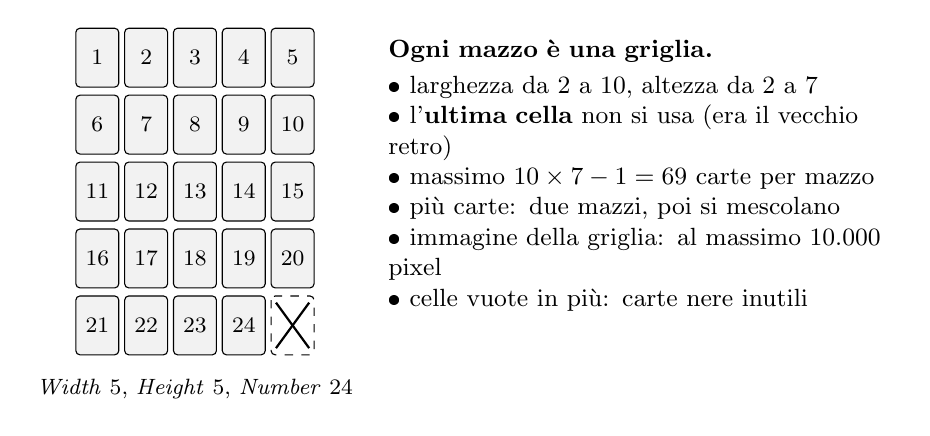
\begin{tikzpicture}[font=\footnotesize, x=0.62cm, y=0.85cm]
  % griglia 5x5
  \foreach \r in {0,...,4} {
    \foreach \c in {0,...,4} {
      \pgfmathtruncatemacro{\n}{\r*5+\c+1}
      \ifnum\n<25
        \draw[fill=gray!10, rounded corners=1.5pt] (\c,-\r) rectangle ++(0.88,-0.88);
        \node at (\c+0.44,-\r-0.44) {\n};
      \else
        \draw[dashed, fill=white, rounded corners=1.5pt] (\c,-\r)
          rectangle ++(0.88,-0.88);
        \draw[thick] (\c+0.1,-\r-0.1) -- (\c+0.78,-\r-0.78);
        \draw[thick] (\c+0.78,-\r-0.1) -- (\c+0.1,-\r-0.78);
      \fi
    }
  }
  \node[anchor=north, align=center] at (2.44,-5.1) {\emph{Width} 5, \emph{Height} 5,
    \emph{Number} 24};
  % nota a destra
  \node[anchor=west, text width=6.4cm, align=left, font=\small] at (6.2,-2.2) {
    \textbf{Ogni mazzo è una griglia.}\\[2pt]
    \textbullet\ larghezza da 2 a 10, altezza da 2 a 7\\
    \textbullet\ l'\textbf{ultima cella} non si usa (era il vecchio retro)\\
    \textbullet\ massimo $10\times7-1 = 69$ carte per mazzo\\
    \textbullet\ più carte: due mazzi, poi si mescolano\\
    \textbullet\ immagine della griglia: al massimo 10.000 pixel\\
    \textbullet\ celle vuote in più: carte nere inutili};
\end{tikzpicture}
\caption{La griglia di un mazzo custom nell'esempio di Ruggero: $5\times5$, con 24
carte e l'ultima cella inutilizzabile. Ricostruzione schematica.}
\label{a8:fig:griglia}
\end{figure}

\paragraph{I template dei mazzi.} Nella stessa cartella dei template dei dadi ci sono i
\textbf{Deck Templates}, con esempi di griglie (anche qui l'ultima carta non è usata).
Servono a poco: danno carte rettangolari e carte quadrate, ma ``che dimensione sono
queste carte? Io magari ho carte di dimensione diversa, strette e alte. Come
faccio?''. La griglia si può comporre a mano con qualunque programma, anche Photoshop,
mettendo le carte ``a manina una di fianco all'altra'', ``ma impazzite senza se e senza
ma''.

\subsection{Il Deck Editor}
\label{a8:sec:deck-editor}

Per questo, nella cartella \emph{Modding}, alla voce \emph{Deck Builder}, Tabletop
Simulator ha un \textbf{software secondario}: il \textbf{TTS Deck Editor}. Prima
pessima notizia: \textbf{non esiste per Mac}. ``Spero che abbiate dei compagni di gruppo
con Windows''. (E Ruggero ricorda che fare un gioco da tavolo non è obbligatorio:
``potete fare anche giochi pervasivi, LARP, giochi di ruolo''.)

Il Deck Editor ``è questa orripilezza qua, sembra fatto da un ingegnere''. La
procedura che Ruggero mostra (figura~\ref{a8:fig:mazzo}):
\begin{enumerate}
  \item \textbf{Nuovo mazzo}: il programma chiede larghezza e altezza della griglia,
        ``esattamente quelli che TTS ci chiede''. Ruggero sceglie $5\times5$. La
        griglia è ``grigia su grigia'', quindi non si vede (``un altro aspetto della
        brillantezza geniale dei programmatori''): compare solo quando ci si
        trascinano dentro le carte.
  \item Si \textbf{trascinano} le immagini delle carte nella griglia e le si copia
        quante volte serve. Nell'esempio: quattro copie dei numeri dal 2 al 6 e
        quattro Jack, ``a caso, non è un mazzo reale''.
  \item \textbf{File, Save Deck As}: si salva nella propria cartella di lavoro un file
        \texttt{.tsdb} (Ruggero lo chiama ``mazzo''). Ma Tabletop Simulator
        \textbf{non apre i \texttt{.tsdb}}: quel file serve solo a riaprire il mazzo nel
        Deck Editor.
  \item \textbf{File, Export}, con due accorgimenti: \textbf{togliere la spunta da
        Upload Image} (le immagini si caricano a mano, non online) e impostare
        \textbf{Max Deck Size a 10.000}. È ``una \emph{safety measure}'': se le carte
        sono gigantesche, il programma le ridimensiona in modo che la griglia non
        superi i 10.000 pixel, perché ``Tabletop Simulator crasha con le immagini più
        grosse di 10.000 pixel''. Si esporta e si ottiene \textbf{l'immagine della
        griglia}.
  \item In Tabletop Simulator, nel Custom Deck: l'immagine della griglia come fronte
        (in cloud), un retro generico (``questo blu mi va bene''), griglia $5\times5$,
        numero 24.
  \item \textbf{Sideways}: è un'opzione vestigiale, ``non spuntatela''; serviva ai
        vecchi mazzi, che non potevano avere carte orizzontali.
  \item \textbf{Backs is hidden}: \textbf{va spuntata}.
  \item \textbf{Import}, ``ed eccolo qua: abbiamo il nostro mazzo''.
\end{enumerate}

\paragraph{Backs is hidden e le mani.} Ruggero mostra a che cosa serve l'ultima spunta.
Dà delle carte alla propria mano e ad altre mani: le carte esistono, ma lui non vede
che cosa c'è nelle mani altrui. Cambiando colore e passando al giallo, vede il giallo e
non vede più l'arancione. \emph{Backs is hidden} significa questo: quando una persona
ha una carta in mano, quella carta è nascosta, e nelle mani degli altri si vede
\textbf{il retro} delle carte anziché il fronte.

\begin{figure}[htbp]
\centering
\begin{tikzpicture}[
    font=\small,
    passo/.style={draw, thick, rounded corners, text width=3.3cm, align=center,
      minimum height=1.25cm, fill=gray!10},
    file/.style={draw, dashed, rounded corners, text width=2.5cm, align=center,
      minimum height=0.8cm, font=\footnotesize},
    freccia/.style={-{Stealth[length=2.5mm]}, thick}
  ]
  \node[passo] (a) at (0,0) {\textbf{Deck Editor}\\ nuovo mazzo, griglia $W\times H$};
  \node[passo] (b) at (4.2,0) {trascinare e copiare le \textbf{carte}};
  \node[passo] (c) at (8.4,0) {\textbf{Export}: niente Upload Image, Max Deck Size
    10.000};
  \node[passo] (d) at (8.4,-2.4) {\textbf{TTS}, Custom Deck: fronte (cloud), retro,
    $W$, $H$, numero};
  \node[passo] (e) at (4.2,-2.4) {Sideways \textbf{no}, Backs is hidden
    \textbf{sì}, Unique Backs se serve};
  \node[passo] (f) at (0,-2.4) {\textbf{Import}: il mazzo è sul tavolo};
  \node[file] (s) at (4.2,1.6) {\texttt{.tsdb}: si riapre solo nel Deck Editor};
  \draw[freccia] (a) -- (b);
  \draw[freccia] (b) -- (c);
  \draw[freccia] (c) -- (d);
  \draw[freccia] (d) -- (e);
  \draw[freccia] (e) -- (f);
  \draw[freccia, dashed] (b) -- node[right, font=\footnotesize] {Save Deck As} (s);
\end{tikzpicture}
\caption{Il flusso di lavoro per creare un mazzo custom, come lo mostra Ruggero. Il
file \texttt{.tsdb} conserva il mazzo per le modifiche successive; a Tabletop
Simulator serve l'immagine esportata.}
\label{a8:fig:mazzo}
\end{figure}

\subsection{Le domande di Gianmarco}
\label{a8:sec:mazzo-domande}

\paragraph{Gli angoli arrotondati.} Gianmarco si è perso una cosa: l'arrotondamento
degli angoli delle carte l'ha fatto Ruggero nelle immagini? Sì e no. Ruggero ha
scaricato da internet un kit di carte singole, ``ce ne sono mille online'', già con gli
angoli arrotondati; ma nelle opzioni custom le carte sono impostate come arrotondate.
Impostandole rettangolari senza arrotondamento, gli angoli diventano neri, perché il
software riempie con il nero la trasparenza dell'immagine. Quando invece le si imposta
arrotondate, è il software ad arrotondarle ``a manina'', e infatti l'arrotondamento
del mazzo è un po' meno accentuato di quello delle immagini.

\paragraph{Più celle che carte.} ``È una domanda veramente stupida'': che cosa succede
se si mette una griglia $6\times6$ e poi un numero diverso dalle carte reali? Ruggero
lo mostra sul $5\times5$, impostando 35 carte: ``ti dà carte nere che non servono''.

\subsection{Carte con retri diversi}
\label{a8:sec:retri}

Finora le carte avevano tutte lo stesso retro. Per un mazzo in cui \textbf{ogni carta
ha il suo retro}: Ruggero copia il file \texttt{.tsdb} (``lo chiamo mazzo retro, così
lavoriamo su un mazzo diverso'') e vi compone la versione ``dark'' delle stesse carte,
nelle stesse posizioni (i numeri dal 2 al 6 neri, e il Jack). Nel Custom Deck, come
fronte resta la griglia di prima; come retro si carica la \textbf{seconda griglia, che
dev'essere identica} nella disposizione; si spunta \textbf{Unique Backs}. Importato, il
mazzo ha ``ognuna il suo retro''. È anche la risposta alla domanda di uno studente sulle
carte a doppia faccia, come quelle di \emph{Taboo}\footnote{``Tabu'' nella
trascrizione.}.

\subsection{La carta singola e le carte bucate}
\label{a8:sec:bucate}

\paragraph{La carta singola.} Il \textbf{Custom Card} chiede semplicemente fronte e
retro, ``senza tutto il resto''. Ruggero crea una carta con il re bianco davanti e il re
nero dietro: una carta singola, che si può mettere insieme alle altre.

\paragraph{Si possono bucare le carte?} Una studentessa chiede se le carte possono essere
forate, ``tipo una sorta di stencil''\footnote{La trascrizione dice ``una sorta di
stendarda'' e poi ``una sorta di scherzo''; dal seguito si capisce che si parla di
carte con dei fori, attraverso cui si vede ciò che sta sotto.}. Sì, perché Tabletop
Simulator gestisce la trasparenza. Ruggero copia il re, lo apre in Photoshop (``per
bucare le cose sono più comodo'') e ci fa un buco e un taglio scanalato di fianco;
basta un qualunque PNG con della trasparenza. Ricaricata, la carta \textbf{è bucata}:
si vede attraverso. ``Attenzione, però'': è bucata \textbf{l'immagine}, ma non è
bucata la \textbf{collisione}; un oggetto appoggiato sopra il buco non ci passa. E
il retro può anche non essere bucato: Ruggero ha bucato solo uno dei due lati, ``una
carta che non può esistere fisicamente''. La carta ha comunque uno spazio fisico che
non si può cambiare. Se si vogliono carte con uno \textbf{spazio fisico bucato}, si
usa il \textbf{token}, che gestisce la trasparenza \emph{anche} nella collisione: un
token ingrandito, appoggiato su un altro oggetto, non collide dove è trasparente.

% ---------------------------------------------------------------------
\section{Il tabellone senza cornice}
\label{a8:sec:tabellone}

Resta il problema della plancia con la cornice di legno
(sezione~\ref{a8:sec:plance}). ``Già lo sapete a questo punto come si fanno i
tabelloni'': \textbf{non li si importa come plance, li si importa come token}. Si crea
un token con una \textbf{profondità molto bassa}, gli si dà l'immagine del tabellone,
lo si ingrandisce in formato tabellone e lo si \textbf{blocca} sul tavolo. ``Anche se
tecnicamente, per TTS, è un token, questa per noi è una plancia''.

\paragraph{La prima pausa.} ``Ora vi darei forse dei minuti di pausa prima di passare
alla prossima fase, se vi va''. ``Se non è già troppo tardi, forse vi ho già consumato
troppo''. Pausa di sette minuti: si riprende alle \textbf{18:40}.

% ---------------------------------------------------------------------
\section{Penna, testo e fogli di carta}
\label{a8:sec:penna}

Al rientro Tiziana saluta (``nessun problema, Tiziana, va benissimo'') e, a quanto
si capisce, lascia la lezione. Ruggero riapre alle domande su quanto visto finora:
caricare componenti, aggiungerli al tavolo.

\paragraph{Esistono delle penne?} Una studentessa chiede se esistono delle penne, per i
giochi in cui bisogna appuntare dei punti o scrivere delle cose. Sì: c'è lo strumento
\textbf{Draw}, la penna, in alto a sinistra, di cui si può cambiare il colore e con cui
si disegna e si scrive sui componenti. (Ruggero si accorge di non aver ancora
ricondiviso lo schermo dopo la pausa: ``giustamente, se no non vedete''.) Ma la penna
non è un componente che si aggiunge: è uno degli \textbf{strumenti base} di TTS, come
il \emph{Grab} e lo strumento \textbf{Testo}. Sono strumenti usati solo nei giochi che
li richiedono, per esempio i \emph{party game} in cui si disegna.

\paragraph{Il foglio di carta.} Quello che manca è il foglio. Ma il foglio può essere
un \textbf{tile} o un \textbf{token bianco} su cui si disegna con la penna nera; oppure
si può usare una texture di carta. O, ancora, si apre un \textbf{tavolo custom} con una
texture bianca: allora ``tutto il tavolo è il nostro tabellone''.

% ---------------------------------------------------------------------
\section{Salvare e pubblicare il modulo}
\label{a8:sec:workshop}

Il modulo ha luce, tavolo, sfondo e componenti. Come lo si salva?

\paragraph{Save \& Load: solo in locale.} La prima opzione è nel menu \textbf{Games},
alla voce \textbf{Save \& Load}. Ruggero salva il modulo come ``Prototipo''; il
salvataggio compare nell'elenco e, cliccandoci, ricarica il modulo così com'era, anche
dopo aver cambiato stanza: ``si ricorda tutto quello che c'era''. Ma un salvataggio è
\textbf{usabile solo in locale}: non lo si può mandare a un \emph{publisher} perché lo
valuti. Per questo bisogna caricarlo come modulo sul \textbf{Workshop} di Steam, ``e
fare questa cosa è un po' più complesso''.

\subsection{Upload e Update}
\label{a8:sec:upload}

Dal menu \textbf{Modding}, la voce \textbf{Workshop Upload} apre una finestra con due
schede:
\begin{description}
  \item[Upload Workshop] si usa \textbf{solo la prima volta} che si carica il
        modulo;
  \item[Update Workshop] si usa per \textbf{tutti gli aggiornamenti} successivi, ``ed
        è più semplice''.
\end{description}

\paragraph{Le informazioni del modulo.} Prima di caricare conviene compilare le
\textbf{Info} del modulo (dal menu del gioco): nome, tipologia, complessità, tempo di
gioco, numero di giocatori, \emph{tag} del Workshop. ``Queste sono informazioni
meccaniche del Workshop''. Ruggero imposta: tipo \emph{game}, complessità bassa,
30--60 minuti, da 2 a 4 giocatori, nome ``prototipo brutto''. (Nel farlo, si accorge di
aver aggiunto per sbaglio un modulo: ``è un inferno, adesso''.)

\paragraph{Il caricamento.} Nell'Upload si scrivono il \textbf{titolo} (``prototipo
brutto''), una \textbf{descrizione} (``quello che volete, lasciamola uguale al
titolo'') e un'\textbf{immagine di anteprima}: ``mi sembra \emph{fitting} metterci la
texture del legno''. Si fa Upload; dopo qualche secondo compare in alto una scritta
verde: il modulo è caricato. Un \emph{pop-up} mostra un numero, l'identificativo del
Workshop, e raccomanda di conservarlo. ``Non ce ne frega niente'': si recupera quando
si vuole, ``non dobbiamo salvarlo o esplodere il mondo''.

\paragraph{La pagina del Workshop.} Nella libreria di Steam, su Tabletop Simulator, c'è
la voce \textbf{Workshop}; da lì, \textbf{i tuoi oggetti}, \textbf{oggetti
pubblicati}. C'è ``prototipo brutto'', con la sua pagina, ``esattamente come le
altre, solo che più brutta'', con il tasto \textbf{Iscriviti} come gli altri moduli.
In alto, però, c'è scritto che la visibilità attuale è \textbf{nascosta}: solo l'autore
può vederlo.

\subsection{La visibilità: unlisted}
\label{a8:sec:visibilita}

Dalla pagina si cambia la visibilità: \textbf{pubblico}, \textbf{solo amici},
\textbf{non in elenco} (\emph{unlisted}), \textbf{nascosto}. Le opzioni che servono sono
due; ``le altre sono delle mezze vie che non servono a nessuno''.
\begin{description}
  \item[Pubblico:] chiunque può entrare nel modulo, guardarlo, copiare le cose,
        prendere i componenti, salvarsi oggetti e immagini.
  \item[Unlisted:] lo vede solo chi riceve il \textbf{link diretto}. L'URL del modulo
        è in alto nella pagina; oppure, tasto destro sullo sfondo, \emph{Copia URL
        della pagina}.
\end{description}
\textbf{Per questo corso, i moduli si pubblicano unlisted}, ``se dovete farlo''. La
pagina del Workshop si può modificare come quelle degli altri giochi (Ruggero ne apre
una come esempio): descrizione, titolo, altre immagini, screenshot, ``paro paro''.

\begin{figure}[htbp]
\centering
\begin{tikzpicture}[
    font=\small,
    passo/.style={draw, thick, rounded corners, text width=2.7cm, align=center,
      minimum height=1.3cm, fill=gray!10},
    locale/.style={draw, dashed, rounded corners, text width=2.7cm, align=center,
      minimum height=1.3cm},
    freccia/.style={-{Stealth[length=2.5mm]}, thick}
  ]
  \node[locale] (s) at (0,1.8) {\textbf{Save \& Load}\\ \footnotesize solo sul proprio
    computer};
  \node[passo] (i) at (0,0) {\textbf{Info}: nome, tipo, complessità, tempo,
    giocatori};
  \node[passo] (u) at (3.5,0) {\textbf{Workshop Upload}: titolo, descrizione,
    anteprima};
  \node[passo] (p) at (7.0,0) {Steam: \textbf{pagina} del modulo (nascosto)};
  \node[passo] (v) at (10.5,0) {visibilità \textbf{unlisted}: si condivide il
    link};
  \node[locale] (up) at (3.5,-2.0) {\textbf{Workshop Update}\\ \footnotesize per ogni
    modifica successiva};
  \draw[freccia] (i) -- (u);
  \draw[freccia] (u) -- (p);
  \draw[freccia] (p) -- (v);
  \draw[freccia, dashed] (up) -- (u);
\end{tikzpicture}
\caption{Dal salvataggio locale al modulo condivisibile, secondo la procedura di
Ruggero. La prima pubblicazione si fa con l'Upload, tutte le successive con l'Update.}
\label{a8:fig:workshop}
\end{figure}

% ---------------------------------------------------------------------
\section{Prendere i componenti degli altri}
\label{a8:sec:riuso}

\paragraph{Save Object.} Una studentessa chiede: quindi chiunque potrebbe prendere i
componenti di altri giochi, se li si fa pubblici? ``Ah, sì, certo. Anzi, adesso arrivo
a parlarvi di questo''. Se serve un componente particolare trovato in un altro modulo,
lo si può salvare. Ruggero apre un modulo pubblico\footnote{``Farm Race'' nella
trascrizione: il titolo del modulo non è verificabile.} che ha dei token a forma di
animale e prende una \textbf{gallina}: tasto destro, \textbf{Save Object}, e la si
chiama ``gallina''. Tornati nel proprio modulo, dal menu Oggetti c'è l'ultima voce che
non aveva ancora nominato, \textbf{Oggetti salvati}: la gallina è lì. ``Così come io
ho salvato un granchio col coltello, per esempio. Può sempre essere utile''. ``Ho anche
un granchio senza coltello''.

\paragraph{Dove finiscono gli oggetti salvati.} Una studentessa ha salvato un mazzo di
carte, con immagini caricate da lei, ma non lo trova più. Se ha fatto un \emph{Save
Object}, dovrebbe trovarlo negli oggetti salvati; caricare le immagini da qualche parte,
da sola, non salva l'oggetto. In ogni caso, \textbf{tutto quello che si è caricato} è
nel menu \textbf{Modding}, alla voce \textbf{Cloud Manager}. È anche buona pratica
farci un po' di pulizia.

\subsection{Quando la sorgente sparisce}
\label{a8:sec:sorgente}

Gli oggetti salvati restano utilizzabili \textbf{finché chi ha caricato l'immagine la
tiene online}. Ruggero ha appena cancellato dal cloud un'immagine (una carta,
``lanciata nel sole'') e vuole mostrare che cosa succede: ricaricando il modulo
dovrebbero comparire degli errori. Ma sul suo computer non succede, perché le immagini
sono ancora nella \emph{cache}, e per svuotarla dovrebbe chiudere e riaprire il software
(``non ho voglia''). Allora condivide il link del Workshop perché qualcuno lo provi.

\paragraph{Discord, non la chat.} Prova a scrivere il link nella chat della lezione;
``No, su Discord, Ruggero, altrimenti non possiamo copiarlo e incollarlo''. Ha ragione:
gli anni scorsi non era così, ma la piattaforma ha cambiato le impostazioni di
sicurezza (``con la questione delle IA hanno aumentato le difese, ma verso cosa?
Comunque, questi sono i miei rant''). Uno studente vorrebbe provare a condividere lo
schermo, ma è collegato dal computer aziendale, che non gli permette di installare
Steam. Ruggero allora descrive l'effetto: chi carica un modulo a cui manca la sorgente
di un'immagine vede un \textbf{messaggio di errore rosso} in alto, ripetuto nella chat
del gioco, e il componente può non caricarsi affatto.

\paragraph{La gallina era un modello 3D.} Il caso della gallina è istruttivo. Aprendo
il suo menu custom, si scopre che non è un token: è un \textbf{modello 3D custom}, a cui
qualcuno ha dato una \textbf{mesh}, un'immagine \textbf{diffuse} e un \textbf{collider}.
Per non perderla, bisognerebbe salvare sul proprio computer queste tre cose
separatamente: ``roba da uscirci impazziti''. Quindi: \textbf{attenzione a che cosa si
salva}, e da dove viene.

\paragraph{I moduli di meeple.} Esistono però moduli che fanno ``il lavoro sporco'' per
gli altri. Ruggero ne usava uno ``che era una bomba atomica'', in cui qualcuno aveva
caricato più di cento modelli 3D di \emph{meeple} di forme diverse; lo riapre, il
software va in crash, e quando lo riapre davvero ne è sopravvissuta circa la metà:
``RIP''. Ma cercando ``meeples'' nel Workshop di Tabletop Simulator si trovano vari
moduli che hanno l'unico scopo di fornire segnalini di varie forme\footnote{La
trascrizione cita un modulo che rende con ``Wooden Talker'' e un altro, ``Mipolorama'',
probabilmente un gioco di parole su \emph{meeple}; i titoli esatti non sono
ricostruibili.}: un riccio, un omino col cappello, barche, camion, stivali, ``tutti
ricolorabili''. ``Avete l'imbarazzo della scelta''.

% ---------------------------------------------------------------------
\section{I moduli di Ruggero}
\label{a8:sec:moduli}

``Ora vi faccio vedere cosa si può fare su Tabletop Simulator quando si lavora per fare
dei moduli'': i moduli che Ruggero ha fatto in passato, ``dai più \emph{easy} ai più
complessi''.

\subsection{Un gioco di carte}
\label{a8:sec:mod-carte}

Il primo è un gioco ``molto \emph{card based}'' fatto per un lavoro\footnote{La
trascrizione dice ``quando lavoravo per Camon''; il nome del committente non è
ricostruibile.}. C'è il \textbf{regolamento} in alto, che si apre a doppia pagina;
\textbf{nove mazzi} di carte; un \textbf{tabellone} con i segnalini che segnano le
risorse e che \textbf{scattano in posizione} (``non stanno a metà via''); sacchetti con
i dadi; plance con i tracciati e i segnalini delle risorse. ``Liscio, regolare: tutte
cose che in teoria dovreste già saper fare anche voi''.

Ruggero ne approfitta per interrogare la classe:
\begin{itemize}
  \item La \textbf{bandiera}, che componente è? Un \textbf{token}, perché ha una forma
        non regolare; e infatti, girata, è specchiata dietro. Lo stesso vale per un
        segnalino col numero 5, specchiato sul retro.
  \item Questi segnalini rotondi? Sono \textbf{tile} rotondi: il retro non è
        specchiato.
  \item La \textbf{plancia}? È una tessera.
  \item Le carte sono mazzi custom. Un mazzo è di \textbf{18 carte}: che griglia ha
        usato? Uno studente propone $7\times3$, ``e poi ne butti via due''; un altro
        $10\times2$. È un $10\times2$. Con $7\times3$ si sprecherebbero tre celle
        (21 meno 18), e una comunque non si può usare; $9\times2$ non basta, perché
        l'ultima cella non è usabile; con 18 carte le celle sprecate sono almeno due.
        ``Potevo fare anche un $5\times4$''.
\end{itemize}

\subsection{La demo di un gioco grande}
\label{a8:sec:mod-cyberpunk}

Il secondo è il modulo completo della \textbf{demo} di un gioco da tavolo grande,
legato a \emph{Cyberpunk}\footnote{La trascrizione dice ``il modulo completo della demo
di Cyberpunk. Destiny 7''; più avanti Ruggero cita il suo lavoro su ``Marvel United e
Cyberpunk'' e una cartella ``Cyberpunk'' nel suo Cloud Manager. Il titolo esatto del
gioco non è ricostruibile dalla trascrizione.}, che ci mette un po' a caricare perché
``ha tonnellate di roba'': un tabellone gigantesco con segnalini ovunque, pile di token
di forma custom, miniature su miniature, carte di diversi mazzi. Il \emph{publisher}
voleva anche la \textbf{scatola}, ``perché volevano far vedere quanto bella è la
scatola''; il regolamento è sospeso in aria, ``perché la gente sta male. Richieste del
publisher, ma va bene''. Ci sono token, carte custom con fronte e retro separati: cose
più complesse per forme e quantità, ma che gli studenti sanno ormai fare. Le
\textbf{miniature} invece sono \emph{asset bundle}: quelle no.

\paragraph{Che cosa c'è di strano?} ``Chi la nota?''. Uno studente: non c'è il tavolo.
Esatto: Ruggero usa il \textbf{non-tavolo}, l'opzione \emph{None}. È il motivo
promesso all'inizio (sezione~\ref{a8:sec:tavoli}). Le mani dei giocatori si possono
spostare dove si vuole; e siccome il software è un simulatore fisico, il tavolo lo crea
lui: un \textbf{token gigantesco}, molto piatto e sottile, con una texture, reso
\textbf{non interagibile} e \textbf{bloccato}. La texture sfuma verso il nero, e con lo
sfondo monocromatico nero il bordo del tavolo si confonde con lo sfondo e non si nota.
In streaming si vede poco; cambiando lo sfondo, si vede subito.

\subsection{Gli ancoraggi}
\label{a8:sec:ancoraggi}

Una cosa che Ruggero non ha spiegato, ``perché non vi servirà per questo prototipo'',
sono gli \textbf{snap point}, i \textbf{punti di ancoraggio}. In certe celle, un
segnalino o una carta appoggiati si posizionano da soli nel punto giusto: ``questo
token, quando va avanti, si ferma lì''. Attivando lo strumento degli ancoraggi (un
puntino verde in fondo al menu), si vede che tutti i tracciati del modulo e delle plance
sono ancorati.

\paragraph{Come si fanno.} ``A mano'', spiega Ruggero: si copia l'oggetto più volte, lo
si allinea con lo strumento \textbf{Gizmo}, che dà una precisione maggiore, e quando
una copia è nel punto giusto ci si clicca sopra con lo strumento degli ancoraggi, che
crea un ancoraggio lì: ``questo componente scatterà esattamente qua''. Poi si cancellano
le copie in più, e gli ancoraggi restano. ``Uno sbatti infinito. Però si può fare''.
Gli ancoraggi valgono per un solo tipo di componente? No: li si può dedicare a vari
componenti, anche con dei \textbf{tag}. Ruggero mostra un gioco ``devastante'', in cui
ogni casellina è un ancoraggio per delle piccole buste, e le teste di certi pezzi vanno
ad agganciarsi al loro posto.

\paragraph{Che cosa si chiede al corso.} ``Noi non vi chiediamo questo livello di
pulizia del prototipo''. Ruggero mostra allora un prototipo su cui sta lavorando in
quel periodo: è ancora grezzo, le icone e le grafiche non sono definitive, alcune carte
non hanno ancora l'illustrazione (``dovrebbe avere una grafica, ok? È un prototipo'').
``Non è neanche questo quello che ci aspettiamo da voi''.

\subsection{Un gioco di ruolo con lo scripting}
\label{a8:sec:mod-gdr}

Tabletop Simulator non è solo per i \emph{board game}: si possono fare anche giochi di
ruolo. Ruggero mostra un modulo fatto per un gioco di ruolo\footnote{La trascrizione
lo chiama ``Magic of the Inventory''; il titolo non è verificabile.}, in cui si è dovuto
usare lo \textbf{scripting}: per esempio, bisognava poter scrivere la descrizione degli
oggetti, quindi le carte sono \textbf{scrivibili}, e certi componenti permettono di
cambiare i numeri.

\paragraph{Non è obbligatorio.} Tornando al ``prototipo brutto'', Ruggero ripete che
Tabletop Simulator probabilmente non servirà a tutti i gruppi: servirà a chi fa giochi
da tavolo, magari un po' ibridi. \textbf{Non è obbligatorio} per il corso; ma per chi è
interessato ai \emph{board game}, è il software usato nel settore.

% ---------------------------------------------------------------------
\section{Perché proprio Tabletop Simulator}
\label{a8:sec:alternative}

Una domanda ``molto laterale'': quanto è legato il settore a Tabletop Simulator? Se
uscisse un simulatore molto migliore, lo si adotterebbe? Ne sono già usciti altri,
risponde Ruggero, per esempio \textbf{Tabletopia}, ma ``sono tutti peggiori in termini
di usabilità''. Tabletopia è gratuito, ``ma fa schifo'', e infatti lo usano in
pochissimi, perché non ha la metà delle funzioni di Tabletop Simulator\footnote{La
trascrizione dice ``non ha la metà delle funzioni che Tabletopia ha'': dal contesto è
evidente che il confronto è con Tabletop Simulator.}.

\paragraph{Le funzioni che non ha mostrato.} E Ruggero, ``per semplicità e per non
farvi impazzire'', ha taciuto cose molto più tecniche:
\begin{itemize}
  \item si possono \textbf{creare nuove mani}, o ridimensionarle: una mano rossa
        molto più grande (``di boh, 30''), per un gioco in cui si tengono in mano
        tantissime carte;
  \item si possono \textbf{incollare} i componenti tra loro con lo strumento della
        \textbf{catenella} (i \emph{joint}): un dado ingrandito incollato sopra un
        cubetto diventa un oggetto solo;
  \item si possono fare \textbf{plance con alloggiamenti}, ancorati, in cui inserire
        altri componenti: Ruggero ne mostra un vecchio prototipo (``è brutto,
        ignoratelo'');
  \item si possono giocare anche i \textbf{legacy}, grazie allo strumento degli
        \textbf{adesivi}: Ruggero crea un adesivo con la sua ``A'' e lo attacca a una
        carta (prima, per sbaglio, sul mazzo intero: ``sono scemo''); la carta,
        mescolata con le altre, conserva l'adesivo.
\end{itemize}
``È che abbiamo una quantità di strumenti qua dentro che è delirante. Non ve ne ho fatti
vedere neanche la metà, vi giuro'': l'angolo di rotazione, l'altezza a cui si
sollevano gli oggetti, ``tutte cose tecniche che non vi servono adesso, ma in cui, se
imparate questo software, c'è un \emph{rabbit hole}''. Non è possibile comprimerlo in
tre ore. L'obiettivo di oggi è dare ``il minimo necessario per riuscire a fare un gioco
che abbia dei componenti, dei dadi, delle carte, un tabellone, una plancia''; per le
idee strambe, si scrive a Ruggero.

\paragraph{Cancellare il modulo.} Ultima procedura: come si cancella un modulo? ``Il
prototipo è troppo brutto per tenerlo''. Dalla pagina del Workshop, in fondo,
\textbf{Elimina}: il modulo viene cancellato dal Workshop, ma non del tutto, perché
resta il \textbf{salvataggio} locale. Cancellato anche quello, ``se ne va via tutto''.

% ---------------------------------------------------------------------
\section{Prototipi in scala}
\label{a8:sec:scala}

Ruggero apre alle domande: ``questa ultima parte della lezione è per rispondere a voi''.
Uno studente, ``per curiosità'': quanto sono verosimili i prototipi che Ruggero
prepara per i \emph{publisher}? Lo scopo è arrivare a una prova realistica?

\paragraph{Estremamente accurati.} ``Quelli che faccio io sono estremamente
accurati'': i componenti sono davvero \textbf{in scala}. Quelle carte sono in formato
poker, 88 mm; quelle altre nel formato delle carte di \emph{Dixit}\footnote{``Le carte
formato di exit'' nella trascrizione: con ogni probabilità \emph{Dixit}, le cui carte
grandi sono un formato standard del settore.}; le miniature hanno la base delle
dimensioni delle miniature reali. Il motivo è il \emph{playtest}: i componenti devono
essere ``il più simulati possibile'' per avere un playtest vicino a quello reale,
perché il playtest verifica anche \textbf{gli spazi}. ``Mettiamo che io ho un distretto,
e devo sapere se ci stanno otto miniature in questo distretto. Come faccio a saperlo,
se io non le muovo?''. Un playtest deve poter dire: ``un po' strettine, ma ci stanno''.
E se gli spazi del tabellone devono contenere le carte, le carte devono essere in scala
con il tabellone, e così i token e le miniature: ``per forza di cose si va a creare
tutto in dimensioni reali''.

\paragraph{Si parte dal tabellone.} Anche prima, nei primi prototipi, il passaggio non
è diverso. Ruggero parte di solito \textbf{dal tabellone}, perché è la cosa più grande
e quindi la più facile da mettere in scala. Tabletop Simulator misura in griglia, in
pollici o in centimetri, \textbf{non in millimetri}: si lavora con i decimali dei
centimetri, e su una carta che misura ``8 virgola qualcosa'' è difficile capire se sia
88, 89, 85 o 86 mm. Su un tabellone di 350 mm l'errore pesa molto meno. Quindi: prima
il tabellone, poi tutto il resto in scala rispetto al tabellone.

\paragraph{Approfondimento: la fedeltà del prototipo.} La risposta di Ruggero mostra
che ``prototipo grezzo'' e ``prototipo in scala'' non sono in contraddizione. Il
prototipo che ha mostrato poco prima ha grafiche provvisorie e carte senza
illustrazione, ma le misure sono già quelle vere: la fedeltà \emph{grafica} è bassa,
quella \emph{spaziale} è alta, perché è lo spazio che il playtest deve verificare.
È lo stesso principio per cui Schell raccomanda di decidere, prima di costruire un
prototipo, quali domande deve aiutare a risolvere: quello che non serve a rispondere
può restare grezzo.

% ---------------------------------------------------------------------
\section{Aggiornare un mazzo e tenere in ordine il cloud}
\label{a8:sec:aggiornare}

\paragraph{Correggere una carta.} L'ultima domanda dello stesso studente è ``più
tecnica'': nei prototipi capita di dover correggere una carta. ``Ottima domanda, ottima
domanda''. Ruggero riprende il mazzo fatto prima e finge un errore di bilanciamento:
invece di due Jack servono, ``che so, due Jack e due regine''. Aggiorna il mazzo nel
Deck Editor, lo salva, lo \textbf{riesporta}, e nel menu custom del mazzo ricarica
\textbf{solo il fronte}, perché il retro non cambia. Con \emph{Search} si vedono le due
regine.

\paragraph{Correggere una sola immagine.} Poi un caso più fine. Ruggero modifica in Paint
una sola carta (la regina di quadri), salvando il file con lo stesso nome. Riaprendo il
\texttt{.tsdb}, il Deck Editor riprende le carte dalla cartella e mostra già la carta
aggiornata. Quindi: \textbf{se si mantengono uguali i nomi dei file}, si aggiorna la
singola immagine, si riesporta nella stessa cartella da cui il \texttt{.tsdb} prende le
carte, e il mazzo è aggiornato senza ricomporlo. ``Anche perché questi moduli si
aggiornano tante volte'': il modulo del gioco che Ruggero sta per pubblicare\footnote{La
trascrizione lo chiama ``Astronega'' e poi ``Astronica''; il titolo non è
ricostruibile con certezza.} è stato aggiornato \textbf{79 volte}. È quello con la
carta senza illustrazione: ``appena l'illustratore me la finisce, io riaggiorno
semplicemente quel file lì, e siamo a posto''.

\paragraph{Le cartelle nel Cloud Manager.} Una buona pratica: caricare le immagini in
cloud \textbf{dentro delle cartelle}. Nel suo Cloud Manager Ruggero ha una cartella per
ogni progetto: tutti i componenti del gioco di \emph{Cyberpunk} in una, quelli
dell'altro gioco in un'altra. ``Dividervi in cartelle vi serve anche per sanità
mentale'', altrimenti ci si ritrova con ``una sfilza di tutte le immagini che avete
usato, caricate a caso''.

\paragraph{Il limite dei 9.999 file.} Ed è buona pratica \textbf{cancellare} ciò che
non si userà. Non è un problema di oggi, ma Tabletop Simulator ha un \textbf{limite
fisso di 9.999 file} caricati. ``Sembrano tanti, e sono tanti se fate pochi giochi. Ma
vi giuro che il limite lo si raggiunge. Io l'ho già raggiunto più volte''. E i file si
cancellano \textbf{uno alla volta}, a mano: non c'è un'opzione per cancellarne di più.
``Lo so: sono pazzi''.

% ---------------------------------------------------------------------
\section{Un software di settore suo malgrado}
\label{a8:sec:storia}

\paragraph{Lo stupore di Rita.} Rita è colpita: per un software di questa portata, è
incredibile che manchino cose così elementari. Lei è abituata ai software Adobe, ``a un
altro tipo di possibilità''; ``però è molto interessante. La lezione di oggi mi ha
stimolato un sacco. Credo che starò tutta la notte a provare''. ``È un software
incredibile, Rita'', risponde Ruggero, ma ``fatto da tre appassionati che non hanno
ragionato per diventare un software di settore. Sono diventati un software di settore
contro la loro volontà''.

\paragraph{Le cose stanno cambiando.} Oggi ne guadagnano, e qualcosa si muove: dalla
pagina della comunità su Steam, nelle notizie, Ruggero mostra la \textbf{roadmap} che gli
sviluppatori hanno deciso di pubblicare dall'inizio dell'anno, ``finalmente, dopo dieci
anni e passa di software''. Stanno aggiornando il motore, ``dopo anni che glielo si
chiedeva''. E gli studenti hanno già visto una versione migliorata. Il Custom PDF,
quando Ruggero ha cominciato, \textbf{non esisteva}: si metteva sul tavolo il
\textbf{tablet} e ci si apriva un link al PDF. E se i file erano esportati in
\textbf{CMYK} anziché in \textbf{RGB}, il software andava in crash ``secco''; ora si
limita a dire che non accetta quel tipo di file. ``Per farti capire quanto fuori di
testa era questa gente''.

\paragraph{Studiare i moduli degli altri.} Un consiglio: ora che si sa come sono fatti i
componenti, si può aprire un modulo qualunque e studiarlo. Con tasto destro,
\textbf{Custom}, su un componente, si vede \textbf{che cosa è}: ``questi bellissimi
tokenoni qua cosa sono? Sono dei modelli o sono dei token? Sono dei token, fantastico.
Questi posso rifarli anch'io, so come farli''. Su un modulo aperto come
esempio\footnote{``Sputacular'' nella trascrizione: il titolo non è ricostruibile.} si
vede che certi segnalini sagomati sono token, perché il retro è specchiato.

\paragraph{Il token fronte-retro.} Esiste però un modo per fare token di forma
particolare con il retro \emph{dritto}: \textbf{incollarne due} con la catenella. ``È un
bello sbatti'', e Ruggero non ricorda più in quale modulo l'aveva fatto. Uno studente
chiede di rispiegarlo, e Ruggero lo rifà da zero: si crea un token con una forma
particolare (un \emph{meeple} giallo) e un secondo token con la stessa forma e il retro
voluto (rosso); dal menu \textbf{Options} si attiva la \textbf{griglia}, che allinea i
pezzi con precisione, così che siano nella stessa identica posizione, uno sopra l'altro;
con la \textbf{catenella} li si aggancia; si toglie la griglia. Il risultato è un token
custom con due facce diverse e il retro non specchiato.

% ---------------------------------------------------------------------
\section{Niente script}
\label{a8:sec:script}

Si possono fare ``cose fuori di testa'': \textbf{perni mobili} (\emph{joint}) per
attaccare gli oggetti, e soprattutto \textbf{script} che automatizzino delle cose. Ed è
qui che Ruggero mette l'unico divieto tecnico della lezione: \textbf{in questo corso
gli script non si fanno}. Il motivo si capirà nella lezione sul playtest: ``gli script
vi rendono più complesso testare cose particolari, e quindi remano contro la vostra
procedura di playtest''. E siccome si vuole un playtest utile e strutturato bene,
``quando arriveranno i playtest vi sarà chiaro perché gli script sono un problema''.

\paragraph{Approfondimento: perché l'automazione disturba il playtest.} La lezione sul
playtest è ancora lontana, ma il senso del divieto si può già intuire dalla
sezione~\ref{a8:sec:simulatore}. In un prototipo analogico i giocatori eseguono le
regole a mano, e proprio eseguendole le capiscono, sbagliano, le contestano: sono i
dati che un playtest raccoglie. Uno script che sposta i segnalini o calcola i punteggi
toglie questi momenti dal tavolo e nasconde il carico di gestione che il gioco stampato
avrà davvero. In più, ogni modifica alle regole tra un playtest e l'altro richiederebbe
di riscrivere il codice: il prototipo diventerebbe più lento da cambiare proprio nella
fase in cui deve cambiare più spesso.

\paragraph{La seconda pausa.} ``Abbiamo ancora mezz'ora di domande''. Silenzio: ``Tutto
chiaro? Non è possibile, non posso essermi spiegato così bene''. Uno studente prevede
che la prima volta che darà un modulo a qualcuno ``gli esploderà il computer''.
Ruggero propone un'altra pausa, fino alle \textbf{19:35}: ``liberatevi un attimo il
cervello, mi rendo conto che oggi è stata molto intensa''. Al ritorno risponderà a
domande e curiosità ``anche generali, non solo sul software, a tutto tondo''. Gianmarco
dice che non gli vengono domande; ``ma le domande verranno tra una settimana, tra un
mese. È normale''. Ogni anno qualcuno gli scrive giorni o settimane dopo: si può fare
questa cosa? La risposta è ``sì'', perché Tabletop Simulator ``è magia nera, è un patto
col diavolo'': sì, ma magari bisogna impazzire tre giorni su un modello 3D; oppure sì,
ma bisogna programmare, ``e piuttosto ti tagli le mani''.

% ---------------------------------------------------------------------
\section{Dopo la pausa: scorciatoie, fisica e destrezza}
\label{a8:sec:fisica}

``Rieccoci qua. Allora, come va? Come state? Io, stanco, venerdì pomeriggio, dopo tre
ore di Tabletop''. Se agli studenti ``si spacca tutto in testa'', è normale: ``è
traumatico''. Quando Ruggero ha cominciato a usarlo, ``odiarlo'' era un eufemismo: non
c'era la metà delle funzioni di oggi ed era molto più complesso. Ma ha ``tante cose
molto funzionali''.

\paragraph{Ingrandire.} Alcune cose da tutorial, che non ha mostrato: con il tasto
\texttt{Alt} si \textbf{ingrandiscono a schermo} le carte e gli oggetti; con il tasto
\texttt{M} si attiva la \textbf{lente} (\emph{Magnify}). (Uno studente gli fa notare
che non sta condividendo lo schermo: ``giusto, hai ragione. In effetti sono pazzo''.)
Dal menu di \texttt{Esc} ci sono tutte le scorciatoie.

\paragraph{La fisica dei componenti.} Ruggero non è entrato nel dettaglio del
\textbf{peso} delle cose: si può cambiare la fisica dei componenti, la \textbf{massa},
l'\textbf{attrito} con l'aria, l'attrito angolare\footnote{``La tritangolare'' nella
trascrizione; si intende con ogni probabilità l'attrito (o la resistenza) angolare,
che regola quanto un oggetto continua a ruotare.}, e perfino la \textbf{gravità} del
modulo. Lo mostra tirando dei dadi con la gravità bassissima e poi altissima. Serve,
per esempio, a fare dei \emph{dexterity game}.

\paragraph{Il minigolf.} La gente usa il software ``per fare le cose più folli''.
C'era un modulo di \textbf{minigolf}: si prendono le palline, si usa lo strumento
\emph{flick}, ``e ok''. ``La gente sta male. In positivo, chiaramente, in questo caso''.
Su Tabletop Simulator si possono fare giochi da tavolo ``nel senso più tradizionale del
termine'', \emph{wargame}, giochi di miniature, giochi di destrezza: ``ha un potenziale
gigantesco'', che però, con la sua interfaccia ``un po' \emph{cranky}, un po' \emph{old
school}'' e i suoi aspetti vestigiali, spesso non arriva.

% ---------------------------------------------------------------------
\section{Un consiglio: giocate The Box}
\label{a8:sec:thebox}

``Uno dei consigli che do sempre, se volete imparare a usare bene questo software e
volete farlo giocando'': giocare \textbf{\emph{The Box}}. È un gioco che \textbf{esiste
solo su Tabletop Simulator}, che ``non può esistere nella realtà per mille motivi che
vedrete se lo giocherete''. Ruggero lo apre, lo linka su Discord, e lo consiglia ``a
prescindere dal corso''.

\paragraph{Perché giocarlo.} ``Come paradigma di game design, questo gioco vi dà una
mano''. È un gioco ``che sulla carta non dovrebbe funzionare'', con un game design che
Ruggero trova ``anche brutto'', ma con ``un'esperienza incredibile da giocare''. E
ragionare sul perché un gioco fatto male dia un'esperienza che può essere molto
positiva ``è molto utile, lato game design''.

\paragraph{Come giocarlo.} ``Non leggetevi niente''. Si organizza una serata (tiene
fino a otto persone, ``se non ricordo male''), si apre un tavolo su TTS e si legge il
regolamento lì: è ``una manciata di pagine'', scritto ``in font gigantesco'', ``non è
bello da vedere''. Il gioco è ``bizzarro, strano'': tre scatole, una delle quali ne
contiene altre \textbf{80}, e un'altra altre \textbf{121}, con nomi bizzarri come
``B126'' o ``diametro infinito''. E fa interagire con moltissimi dei componenti visti a
lezione: è l'opzione consigliata per ``prendere confidenza con la varietà più disparata
di componenti''. (``Adesso che ve l'ho nominato, devo organizzare per giocarlo con
qualcuno, perché è bellissimo''.)

\paragraph{Approfondimento: imparare da un gioco ``brutto''.} Il consiglio di Ruggero
riprende un'idea che attraversa tutto il corso: l'esperienza del giocatore non coincide
con la qualità ``sulla carta'' delle regole. Nel lessico dei framework visti nelle
lezioni precedenti, un insieme di meccaniche discutibile può comunque produrre
dinamiche e un'esperienza memorabili, e capire \emph{perché} succede è un esercizio di
analisi più istruttivo che studiare un gioco ben fatto. Schell lo formula come
un'abitudine del designer: guardare all'esperienza prima che alle regole, e chiedersi
quali elementi la producono davvero.

% ---------------------------------------------------------------------
\section{Saturi}
\label{a8:sec:saturi}

``Oltre a TTS, come state?''. Una studentessa è ``saturatissima'' di cose apprese: deve
``fare un attimo ordine fra i pensieri'' per capire che cosa provare per prima e che
cosa chiedere. ``Certamente''; e di nuovo, a Ruggero si può scrivere per mail o su
Telegram. Un'altra è ``satura di nozioni, non riesco più ad apprendere''. Rita
ringrazia: ``è la lezione più bella finora per me''.

Ruggero è contento: questa lezione, per molti, è ``una mattonata''. Le classi sono
molto diverse, e capitano studenti che non hanno mai avuto confidenza con software
tecnici, per cui questa lezione ``è un po' una mazzata''; ``sono contento, Rita, che ti
sia piaciuta, anche perché abbiamo davvero sorvolato la punta dell'iceberg di Tabletop
Simulator, questo ve lo assicuro''.

% ---------------------------------------------------------------------
\section{Il playtest e il calendario del corso}
\label{a8:sec:calendario}

Una studentessa (``sempre le mie domande\ldots''): quanto è rilevante usare Tabletop
Simulator nel \emph{playtest}, e quanto invece è importante farlo \textbf{fisico}? ``Ti
sorprenderà sapere'' che c'è una lezione sul playtest. ``Immaginavo'', risponde lei, ``ma
lo faccio apposta: tu mi anticipi ogni volta le cose''; e, come ha visto, nelle lezioni
successive le cose vengono riprese.

Ruggero controlla quando, e già che c'è ripassa il resto del calendario
(tabella~\ref{a8:tab:calendario}).

\begin{table}[htbp]
\centering
\small
\begin{tabular}{@{}p{3.0cm}p{9.6cm}@{}}
\toprule
\textbf{Quando} & \textbf{Che cosa} \\
\midrule
lunedì (5 ottobre) & lezione con Beatrice, la seconda sulle \textbf{esperienze
ludiche} \\
venerdì (9 ottobre) & lezione sul \textbf{paragame}\protect\footnotemark, ``una delle
mie preferite''; si parlerà anche di TTS, ``ma a tangente'' \\
12 ottobre & il \textbf{pitch}: niente lezione, il \emph{check} dei progetti \\
fino a novembre & periodo di lavoro senza lezioni \\
6 novembre & lezione con \textbf{Diego} sull'\textbf{RNG} (la casualità) \\
9 novembre & \textbf{playtest} con Ruggero: ``playtest e metodi etnografici di raccolta
feedback'' \\
dopo & \textbf{gioco di ruolo da tavolo} con Daniele \\
dopo & ``l'ondata lunga'' di \textbf{sviluppo 1} e \textbf{sviluppo 2} con
\textbf{Marta}: \emph{development}, modelli matematici, bilanciamento e altri aspetti
dello sviluppo \\
dopo & \textbf{produzione} con \textbf{Flavio} \\
dopo & altro periodo di lavoro \\
11 dicembre & \textbf{final review} \\
dopo la review & \textbf{tavola rotonda} con editori e persone del settore \\
\bottomrule
\end{tabular}
\caption{Il calendario del resto del corso come lo ripassa Ruggero. Le date tra
parentesi sono ricostruite dal contesto; le altre sono dette a voce.}
\label{a8:tab:calendario}
\end{table}
\footnotetext{La trascrizione dice ``quella sul paragame''; il termine non è spiegato
nella lezione.}

\paragraph{La tavola rotonda.} Dopo la \emph{final review}, nella lezione di
\textbf{tavola rotonda} i docenti portano \textbf{editori} e altre persone del settore
a dare un feedback sui progetti: un punto di vista che non sia solo quello degli
insegnanti, ma di chi lavora nel settore. Gli ospiti si scelgono \textbf{in base ai
giochi dei gruppi}. L'anno scorso, ``per varie cose'', non è uscito neanche un
\emph{board game}: giochi di ruolo, LARP, giochi pervasivi, ma nessun gioco da tavolo; e
quindi non sono stati chiamati editori di giochi da tavolo, perché ``non aveva senso
dare feedback da qualcuno che lavora nel board game a un gioco di ruolo''. Anche
quest'anno la tavola rotonda sarà calibrata su quello che i gruppi faranno. La
studentessa aggiunge che finora non ha mai strutturato i prototipi su TTS, li ha sempre
fatti fisici; ``non è un problema''.

% ---------------------------------------------------------------------
\section{Domande e risposte, alla rovescia}
\label{a8:sec:rovescia}

``Avete altre domande, dubbi? Avete risposte? Mi date le risposte, io vi credo''. Uno
studente sta al gioco: ``È blu, è blu, è blu''. E poi: ``come faccio un componente a
goccia?''. Ruggero ricorda un \emph{trend} su Reddit: dare prima le risposte e poi
inventare le domande, in modo che chi ha risposto sembri la persona peggiore possibile
(``la mattina ne mangio due'' --- ``quanti bambini mangi al mattino?''). ``Va bene, non
volevo neanche andarci. Dove stiamo andando?''. La domanda sulla goccia resta senza
risposta (ma si è visto prima come ottenere ``gocce d'acqua'' dalle pietre del Go,
sezione~\ref{a8:sec:misc}, e come fare un token di forma libera,
sezione~\ref{a8:sec:custom-token}).

Mancano 14 minuti. La battuta sui bambini ha inquietato una studentessa, che ha appena
finito di ascoltare \emph{Veleno}\footnote{Il podcast d'inchiesta italiano di Pablo
Trincia; la trascrizione lo rende ``Veleno agli atti''.}: ``è stato un attimo di
infarto''. Sono podcast italiani intensi, ``tostarelli''.

% ---------------------------------------------------------------------
\section{Le risorse da seguire}
\label{a8:sec:risorse}

A proposito di podcast e risorse: Ruggero aveva suggerito delle risorse nelle slide di
una lezione precedente, ma lo studente si è un po' confuso; quali sono i
\emph{must} da seguire su YouTube? Ruggero ne segue diverse, ``ma per motivi molto
diversi'': alcune per i \emph{game studies}, alcune per il game design, alcune per la
grafica.
\begin{description}
  \item[Daniel Solis] è ``molto bravo sulla parte di \emph{graphic design} per i
        board game'': il suo canale è molto tecnico su come progettare una grafica
        \textbf{funzionale} al proprio gioco.
  \item[Amabel Holland] ha ``un buon mix'': fa molta ``quasi archeologia ludica'',
        ricerca storica sui giochi, ma anche video di game design ``molto sul
        pezzo''\footnote{Ruggero cita anche altri ``approcci'' che la trascrizione
        rende in modo incomprensibile (``approcci cosmodiali''): un altro canale tra i
        suoi preferiti, il cui nome non è ricostruibile.}.
  \item[Action Button] è il suo canale preferito in assoluto. Ruggero ha una
        preferenza, ``mi rendo conto mia'', per i video-saggio molto lunghi (``se apro il
        mio YouTube, vedete video da quattro ore e passa''): Action Button analizza
        \textbf{singoli giochi} in video dalle tre alle dieci ore, andando molto a
        fondo non solo sul game design ma sulla \textbf{game culture} e sul
        \textbf{contesto}: in quale epoca il gioco è stato creato, che cosa nel mondo
        reale ha influenzato chi l'ha fatto, perché il gioco è uscito in quella forma.
\end{description}

\paragraph{Il video preferito.} Il suo video preferito in assoluto è quello su
\emph{Tokimeki Memorial}\footnote{``Took Me Me Me Me Me, Key Memorial'' e ``Toki Maki
Memorial'' nella trascrizione.}: ``5 ore e 56 minuti, e lo so a memoria perché è il
video che ho riguardato di più nella vita''. ``Mi rendo conto che è una nicchia di una
nicchia di una nicchia'', e potrebbe non essere per nessuno oltre a lui. È ``un
\emph{roller coaster} emotivo'': se ne esce tristi, arrabbiati, ma anche fiduciosi
nell'umanità, soddisfatti; ``molte cose provi''. Lo studente vede anche un video su
\emph{Final Fantasy VII Remake}, che ha odiato: ``allora amerai quel video!''. Poi lo
studente deve andare e saluta.

\paragraph{Il podcast che non si nomina.} Ruggero aggiunge, imbarazzato, che ha anche
lui un podcast, ``ma fate come se non avessi detto niente''; non lo ha messo nelle slide
perché ``ho sempre imbarazzo sulle cose che faccio''. Una studentessa ha già trovato il
suo canale; lui insiste che non vuole fare ``il prof che consiglia i propri libri'' e
che non parla quasi mai neanche dei suoi giochi. Sul suo sito c'è tutto. Ma il podcast
non ha pubblicità né sponsor, volutamente: ``non mi deve rompere nessuno. È una roba che
faccio per pace mentale mia''. La studentessa (``ho 30 anni, ho già studiato in tanti
campi'') dice di stimarlo proprio per questa scelta: ``tutti invece vogliono fare i
professori per vendere le loro cose'', e questo modo di fare l'ha spinta ancora di più
ad andare a vedere il suo lavoro.

% ---------------------------------------------------------------------
\section{Giochi invendibili e l'economia del gioco}
\label{a8:sec:mercato}

``Io sono l'ultima persona che vi deve dire come comunicare questi giochi'', dice
Ruggero: comunicazione e vendita ``mi fanno schifo'' (lui, ``come anche Daniele e
Beatrice'', non è lì per quello). I giochi che fa nel tempo libero ``sono cose
invendibili''.

\paragraph{``Se volete perdere soldi''.} L'ultimo incontro commerciale in cui ha
proposto a un \emph{publisher} uno dei suoi giochi migliori, gli ha detto: ``se volete
perdere soldi, è l'ideale''. ``È terribile, non si fa''; ma è stato onesto. Ha fatto
quell'incontro con un solo editore, l'unico di cui si fida al punto da proporglielo,
sapendo che gli avrebbe fatto perdere soldi: ``quindi devo essere molto onesto''. Una
studentessa chiede, senza voler sapere i dettagli, se il gioco è stato provato con delle
persone: è ``il mio \emph{magnum opus}'', ed è ``talmente intenso che in un playtest
una persona ha vomitato''. Ma se alle persone piace, obietta lei, ci sarà un pubblico a
cui venderlo.

\paragraph{I numeri del mercato italiano.} La risposta è nella scala economica del
settore, ``molto bizzarra''. In Italia, un gioco da tavolo che vende ``regolarmente''
vende \textbf{tra le mille e le duemila copie}; un editore è già contento se ne vende
\textbf{più di mille}. Il gioco di ruolo è su una scala ancora più bassa: un manuale che
vende \textbf{500 copie} in Italia è già un buon risultato. La fetta maggiore del mercato
va a giochi come \emph{Dungeons \& Dragons}, che lasciano poco spazio al resto. Ruggero
ha lì il suo gioco, perché deve portarlo a un evento il giorno dopo: una scatola
bianca, anonima, senza niente sopra, ``solo io so che gioco è''. ``Se ne vende 50 copie,
sono 49 persone in più di quelle che pensavo potessero prenderlo''.

\paragraph{Sapere perché si fa un gioco.} È il tema della prima lezione, ricorda la
studentessa: bisogna avere chiaro \textbf{perché} si fa un gioco. Quando Ruggero ha
lavorato a \emph{Marvel United} e a \emph{Cyberpunk}, giochi su IP gigantesche, il gioco
doveva essere per il \emph{mass market}, accessibile. Ma con un gioco suo, per scopi
suoi, non commerciali, su cui non deve guadagnare, può fare ``quello che voglio''. ``E
non è un gioco peggiore o meno degno di esistere''. Come nel cinema ci sono i film della
Marvel, i documentari di nicchia e l'horror indipendente che va ai festival. La
studentessa è d'accordo: è un'opera di creatività. Si scusa per averlo messo in
imbarazzo; ``no, sei tu, non sono io che sono inadeguato'', scherza lui.

\paragraph{Approfondimento: obiettivi diversi, giochi diversi.} Lo scambio riprende, dal
punto di vista di un professionista, la distinzione tra l'obiettivo del gioco e
l'obiettivo personale di chi lo fa, che il corso ha affrontato parlando del perché si
fa game design. Un gioco su licenza per il grande pubblico e un gioco personale
``invendibile'' rispondono a obiettivi diversi, e si giudicano con metri diversi: il
primo dall'accessibilità e dalle vendite, il secondo dall'esperienza che riesce a dare
al suo pubblico, per quanto piccolo.

% ---------------------------------------------------------------------
\section{I giochi lunghi}
\label{a8:sec:lunghi}

``Siamo rimasti solo noi tre''. Cinque minuti alla fine. Uno studente non ha una domanda
ma una confessione: vedendolo nello scaffale alle spalle di Ruggero, ha comprato
d'impulso un gioco lungo\footnote{La trascrizione lo rende ``Spichisi'' e ``Speak
easy''; il titolo non è ricostruibile con certezza.} che sa che non giocherà mai,
``perché intavolare questi giochi è sempre un casino''. Neanche Ruggero l'ha ancora
giocato: dura molto, e alle persone non si può mentire: ``guarda, secondo me almeno 4--5
ore siamo qui fissi''.

\paragraph{Un evento per i giochi lunghi.} Lo studente racconta che cosa ha fatto
tornando in Puglia: ha contattato le associazioni del Sud Barese, dove vive, e insieme
hanno creato un \textbf{evento a invito, a porte chiuse}, conosciuto solo dalle
associazioni e riservato ai giocatori, per giocare proprio questi giochi molto lunghi.
La maggior parte delle associazioni lavora con eventi aperti, in cui si fa da
dimostratori dei giochi e non si può giocare davvero: un gioco così non lo si può
portare quando arriva una persona che vede un gioco da tavolo per la prima volta. Il
loro evento dura tutta la giornata, e hanno fatto ``cose abbastanza grosse''; il
prossimo piano era \emph{Here I Stand}\footnote{``Il re stand'' nella trascrizione:
con ogni probabilità \emph{Here I Stand}, gioco storico molto lungo della GMT.}, poi
saltato. Sullo scaffale ci sono diversi titoli della \textbf{GMT}: \emph{Cuba Libre},
\emph{A Distant Plain}, \emph{Fire in the Lake}; e ancora da giocare un titolo
strategico ambientato a Taiwan\footnote{La trascrizione lo chiama ``il 2045, quello
strategico taiwanese''; il titolo non è ricostruibile con certezza.}.

\paragraph{``Si gioca poco''.} ``Il tempo per giocare è poco, c'è poco da fare''. Lo
studente immagina che, facendolo per lavoro, a un certo punto venga la nausea. ``Ma non
esiste''. Ruggero gioca \textbf{400 giochi all'anno} e ne giocherebbe 800, se la gente
venisse a giocare; ``invece, purtroppo, le persone hanno una vita''. La registrazione
si interrompe qui.

% ---------------------------------------------------------------------
\section*{Punti chiave del capitolo}
\addcontentsline{toc}{section}{Punti chiave del capitolo}

\begin{itemize}
  \item Il \textbf{pitch} del 12 ottobre non è commerciale: 40--50 minuti per gruppo
        per fissare un \emph{agreement} su che cosa si farà (tipo di gioco, numero di
        giocatori, esperienza e come darla, durata). Forma libera; nessuna scaletta,
        volutamente.
  \item \textbf{Tabletop Simulator non è un motore per videogiochi}: è un
        \textbf{simulatore fisico} di un tavolo. Ogni oggetto ha massa, spazio,
        collisioni; i componenti vanno trattati come componenti fisici. È il software
        di riferimento del settore, pieno di scelte vestigiali.
  \item I moduli si costruiscono in \textbf{single player}. Le immagini si caricano
        \textbf{da file} (mai da URL) e \textbf{in cloud} (mai in locale).
  \item Il \textbf{tavolo} decide quanti giocatori ci stanno (le \emph{hands}) e come
        si comportano i componenti sui bordi: è una questione di \emph{table presence}.
        Il tavolo custom stira l'immagine; la plancia custom si adatta all'immagine,
        ma ha la cornice di legno.
  \item Lo \textbf{sfondo} cambia la luce: conviene uno sfondo monocromatico da un
        pixel e la luce slegata dallo sfondo, regolando \emph{light}, \emph{ambient}
        e \emph{reflection intensity}.
  \item Per ogni componente: \textbf{esiste già o va creato?} Ricolorare
        (\emph{Color Tint}) non ricolora tutto (i pallini dei dadi). Si lavora
        \textbf{in scala reale}: righello in cm, vista dall'alto, \texttt{+} e
        \texttt{-}. Niente \textbf{sacchetto infinito}: i componenti si devono poter
        contare; il sacchetto normale va in \emph{Random}.
  \item \textbf{Token}: forma libera, trasparenza e collisione, colorabile, impilabile,
        ma retro specchiato. \textbf{Tile}: forme regolari, fronte e retro corretti,
        niente trasparenza. I \textbf{tabelloni} si fanno con un token sottile e
        bloccato.
  \item Il \textbf{dado custom} si fa dai template (UV map) nella cartella
        \emph{Modding} dei file installati, lavorando su una copia.
  \item Il \textbf{mazzo custom} è una \textbf{griglia}: massimo $10\times7$, ultima
        cella inutilizzabile, quindi 69 carte. Si compone con il \textbf{Deck Editor}
        (solo Windows), si esporta senza upload e con \emph{Max Deck Size} 10.000; in
        TTS, \emph{Sideways} no, \emph{Backs is hidden} sì, \emph{Unique Backs} per i
        retri diversi. Mantenendo i nomi dei file si aggiorna una carta sola.
  \item Il salvataggio locale non si condivide: si pubblica sul \textbf{Workshop}
        (Upload la prima volta, poi Update), in \textbf{unlisted} per il corso. I
        componenti altrui si salvano con \emph{Save Object}, ma dipendono da chi li ha
        caricati; il Cloud Manager va tenuto in cartelle (limite di 9.999 file).
  \item I moduli professionali usano il non-tavolo, ancoraggi, componenti in scala
        (si parte dal tabellone); al corso non si chiede quel livello. \textbf{Niente
        script}: remano contro il playtest.
  \item Dalle domande finali: giocare \emph{The Box} per capire il software e per
        riflettere su un gioco ``brutto'' che dà un'esperienza bellissima; seguire
        Daniel Solis, Amabel Holland, Action Button; in Italia un gioco da tavolo che
        vende ne vende mille--duemila copie, un GdR 500: sapere \textbf{perché} si fa
        un gioco cambia il metro con cui lo si giudica.
\end{itemize}

%    % =====================================================================
%  Analog Game Design, lezione 9 — Organizzare la progettazione,
%  giochi formativi ed escape room. In apertura, il giro di come si sta
%  e lo stato dei lavori di gruppo; poi la conclusione delle slide
%  sul project management di un gioco (le risorse: tempi, competenze,
%  energie, risorse economiche e fisiche; il progetto come una game
%  jam; il documento "Project management di un gioco" voce per voce:
%  obiettivo e target, vincoli, tempo e ore, fasi e output attesi, la
%  regola delle ore non tutte allocate, emozioni, meccaniche e flusso,
%  percorso dell'utente, primo prototipo, playtest e iterazione,
%  documentare, monitorare, la stima del tempo e il 20% in più, "semplice
%  è meglio"); poi "Esperienze ludiche 2": il Game Design Document,
%  l'Experience Canvas e le tre grandi domande; gamification e game
%  based learning, motivazione intrinseca ed estrinseca, la volontarietà
%  del gioco e la discussione con Tiziana su Duolingo; Sugata Mitra e
%  l'educazione minimamente invasiva; le escape room formative (tre
%  strutture di enigmi, dove trovare gli enigmi, le indicazioni di un
%  paper); dopo la pausa, la parte burocratica (GDPR, informativa sulla
%  privacy, esonero di responsabilità, proprietà intellettuale); in
%  chiusura, l'Urban Game Deck e un giro di feedback sul corso.
%  Fonte: trascrizione della nona lezione (AGD9) del corso breve di
%  Analog Game Design, seconda edizione: una lezione online di circa
%  tre ore, condotta da Beatrice, con due pause (fino alle 17:36 e
%  dalle 19:16 alle 19:21).
%  Pacchetti richiesti nel preambolo del libro (già presenti nel
%  main.tex): \usepackage{booktabs}, \usepackage{tikz} con
%    \usetikzlibrary{shapes.geometric,shapes.symbols,shapes.misc,
%      arrows.meta,positioning,calc,fit}
%  (le librerie vanno caricate nel preambolo, non nel capitolo).
%  Consigliati, come per gli altri capitoli: \usepackage[italian]{babel}
%  e \usepackage[T1]{fontenc} (il capitolo compila anche senza).
%
%  Collocazione nel libro: parte "Analog Game Design", nono capitolo
%  (numerazione propria 2.9). Nel file principale del libro, subito dopo
%  il capitolo 2.8:
%
%    % =====================================================================
%  Analog Game Design, lezione 8 — Tabletop Simulator: costruire un
%  modulo per il prototipo di un gioco da tavolo. In apertura, le
%  domande sul pitch del 12 ottobre (che cosa si porta, perché non c'è
%  una scaletta); poi la lezione pratica di Ruggero sul software: il
%  menu iniziale, "un gioco da tavolo è un gioco su un tavolo" (TTS è
%  un simulatore fisico, non un motore per videogiochi), i tavoli e la
%  table presence, gli sfondi e la luce, i componenti standard
%  (blocchi, plance, carte, dadi, figurine, sacchetti...), i componenti
%  custom (PDF, token, tile, dado, mazzo con il Deck Editor), il
%  salvataggio e il caricamento sul Workshop di Steam, il riuso dei
%  componenti altrui, i moduli professionali di Ruggero, le funzioni
%  avanzate (ancoraggi, catenella, adesivi, fisica) e il divieto degli
%  script; in coda, le domande libere (fedeltà dei prototipi per i
%  publisher, aggiornare un mazzo, il calendario fino alla final
%  review, The Box, le risorse da seguire, il mercato italiano del
%  gioco, i giochi lunghi).
%  Fonte: trascrizione dell'ottava lezione (AGD8) del corso breve di
%  Analog Game Design, seconda edizione: una lezione online di circa
%  tre ore, condotta da Ruggero, con due pause (fino alle 18:40 e fino
%  alle 19:35).
%  Pacchetti richiesti nel preambolo del libro (già presenti nel
%  main.tex): \usepackage{booktabs}, \usepackage{tikz} con
%    \usetikzlibrary{shapes.geometric,shapes.symbols,shapes.misc,
%      arrows.meta,positioning,calc,fit}
%  (le librerie vanno caricate nel preambolo, non nel capitolo).
%  Consigliati, come per gli altri capitoli: \usepackage[italian]{babel}
%  e \usepackage[T1]{fontenc} (il capitolo compila anche senza).
%
%  Collocazione nel libro: parte "Analog Game Design", ottavo capitolo
%  (numerazione propria 2.8). Nel file principale del libro, subito dopo
%  il capitolo 2.7:
%
%    % =====================================================================
%  Analog Game Design, lezione 7 — Obiettivi di design e design sprint:
%  l'annuncio dei gruppi e del project work (mandate, calendario, pitch
%  del 12 ottobre, regole di lavoro sul Drive); perché si fa game design
%  (obiettivo del gioco e obiettivo personale: pubblicare, esprimersi,
%  formare e sensibilizzare, fare marketing, e le competenze che ognuno
%  richiede); un esercizio di design sprint fatto da tutta la classe su
%  una lavagna di Canva (la chiacchierata iniziale, l'obiettivo del
%  gioco, il racconto delle idee, la votazione a pallini, la ricerca e
%  sviluppo, la mappa impatto-sforzo, il percorso dell'utente, "state
%  sul semplice"); in coda, il primo tutoraggio con Ruggero (emozioni
%  prima delle meccaniche, il gioco del traditore, Tabletop Simulator,
%  che cos'è il pitch, il Mixing Desk come paletti e non come
%  validazione).
%  Fonte: trascrizione della settima lezione (AGD7) del corso breve di
%  Analog Game Design, seconda edizione: una lezione online di circa
%  tre ore (apertura di Daniele, poi Beatrice), con una pausa breve
%  alle 19:10, seguita nello stesso file dalla registrazione del primo
%  tutoraggio di gruppo, un'ora su Meet con Ruggero, tre giorni dopo.
%  Pacchetti richiesti nel preambolo del libro (già presenti nel
%  main.tex): \usepackage{booktabs}, \usepackage{tikz} con
%    \usetikzlibrary{shapes.geometric,shapes.symbols,shapes.misc,
%      arrows.meta,positioning,calc,fit}
%  (le librerie vanno caricate nel preambolo, non nel capitolo).
%  Consigliati, come per gli altri capitoli: \usepackage[italian]{babel}
%  e \usepackage[T1]{fontenc} (il capitolo compila anche senza).
%
%  Collocazione nel libro: parte "Analog Game Design", settimo capitolo
%  (numerazione propria 2.7). Nel file principale del libro, subito dopo
%  il capitolo 2.6:
%
%    \input{AGD/AGD6_ricerca_e_sviluppo}
%    \input{AGD/AGD7_obiettivi_e_design_sprint}
%
%  Tutte le etichette di questo capitolo hanno il prefisso "a7:"
%  (a7:cap:..., a7:sec:..., a7:fig:..., a7:tab:...). Il capitolo è
%  autonomo: non contiene \ref verso altri capitoli.
%  Le figure e le tabelle sono ricostruzioni schematiche di quanto i
%  docenti spiegano a voce, con le slide e sulla lavagna condivisa, non
%  copie delle slide. Le idee degli studenti sono riassunte come le
%  raccontano loro, ripulite dagli errori del riconoscimento vocale;
%  dove la trascrizione è troppo rovinata per ricostruire un dettaglio,
%  il capitolo lo dice invece di inventarlo.
% =====================================================================

\chapter[Obiettivi di design e design sprint]{Obiettivi di design e design
sprint: i gruppi, il perché di un gioco e un primo gioco inventato insieme}
\label{a7:cap:sprint}

Questa è la \textbf{settima lezione} del corso di \textbf{Analog Game Design}, ed è
la lezione in cui il corso cambia passo. Fino a qui gli studenti hanno lavorato da
soli, sui task ``didattici'' (il personaggio, il gioco di ruolo in 200 parole); da
oggi lavoreranno \textbf{in gruppo} sul \textbf{project work}, il gioco analogico
che accompagnerà tutto il resto del corso. La lezione si apre quindi con Daniele,
che annuncia i \textbf{gruppi}, il \emph{mandate} (che cosa si deve fare e che cosa
no), il \textbf{calendario} e le regole pratiche per lavorare. Poi la parola passa a
Beatrice, che fa due cose. La prima è un ``cappellino introduttivo'' su
\textbf{perché si fa game design}: un gioco ha un obiettivo suo, ma anche chi lo fa
ha un \textbf{obiettivo personale} (pubblicare, esprimersi, formare, fare
marketing), e ognuno di questi obiettivi chiede competenze diverse. La seconda, che
occupa la maggior parte del tempo, è un \textbf{esercizio di design sprint}: tutta
la classe finge di essere un unico gruppo di nove persone e, su una lavagna
condivisa, percorre le fasi che porterebbero da zero al \emph{pitch} di un gioco.
L'esercizio produce un vincitore inatteso (``i funghi hanno un sacco di successo,
non me lo immaginavo'') e, soprattutto, un metodo da riusare quando un gruppo si
blocca: timer, post-it, votazione a pallini, ricerca, \textbf{mappa impatto-sforzo},
\textbf{percorso dell'utente}, e la regola d'oro ``\textbf{state sul semplice}''.

La trascrizione contiene anche, in coda, la registrazione del \textbf{primo
tutoraggio}, che il capitolo riporta per intero perché ne è la naturale
prosecuzione: un'ora con \textbf{Ruggero}, tre giorni dopo, ``guidata dalle vostre
domande''. Lì tornano i temi della lezione, visti dall'interno dei gruppi appena
nati: perché partire dalle \textbf{emozioni} e non dalle meccaniche, che cosa ci si
aspetta davvero dal \textbf{pitch} del 12 ottobre, come usare il \textbf{Mixing
Desk} senza farsene schiacciare, e come prepararsi alla lezione su
\textbf{Tabletop Simulator} del giorno dopo.

La lezione è \textbf{online} e ha tre voci. Apre \textbf{Daniele}\footnote{Come
nelle lezioni precedenti, il cognome non è ricostruibile con certezza: qui la
trascrizione lo fa pronunciare a Daniele stesso come ``Daniele Fusetto'' (nella
prima lezione era ``Daniel Cusetto'').}, che resta solo ``per la presentazione dei
gruppi'' e poi si scollega per un'altra riunione; prosegue \textbf{Beatrice}
(``Bea''), che conduce tutta la lezione e l'esercizio; \textbf{Ruggero} non c'è
alla lezione (è nominato più volte, anche come ``Ruger'' e ``Rugger'') ma conduce
il tutoraggio. La lezione si colloca con ogni probabilità \textbf{lunedì 28
settembre 2026}\footnote{La data non è detta, ma è ricostruibile: Daniele parla
della lezione di ``venerdì'' (quella sulla ricerca e sviluppo, del 25 settembre)
come appena passata, ricorda che Gianmarco ``come sempre, lunedì'' arriva verso le
sei, e annuncia il tutoraggio per ``giovedì 1 ottobre''. Nel tutoraggio uno
studente parla della ``lezione di lunedì'' sui funghi e Ruggero osserva ``siamo a
ottobre''.}, dalle 17 alle 20 circa: la pausa è dalle \textbf{19:10} alle
\textbf{19:15}, e la sessione di ricerca finisce alle \textbf{19:32}. Il tutoraggio
è \textbf{giovedì 1 ottobre}, alle 17, su Meet, e dura un'ora. In classe ci sono
\textbf{Tiziana}, \textbf{Rita}, \textbf{Tancredi}, \textbf{Giordano},
\textbf{Angelo}, \textbf{Gianmarco} (che arriva a esercizio iniziato),
\textbf{Nicola} (che arriva ancora più tardi) e i \textbf{due Lorenzo}: Lorenzo
Vergata e l'altro Lorenzo, che durante la lezione propone di farsi chiamare con il
secondo nome, ``John'', per evitare confusioni\footnote{``Non ce la posso fare, i
doppi nomi mi devastano'', dice Beatrice. L'altro Lorenzo spiega che il suo secondo
nome è John, ``non sto scherzando'', e Beatrice se lo appunta come ``Lorenzo L.''.
Nel capitolo lo si chiama ``l'altro Lorenzo''; Lorenzo Vergata è chiamato per nome e
cognome quando serve distinguerli.}.

Tre avvertenze di lettura, le stesse dei capitoli precedenti. La prima: la
trascrizione è automatica e storpia moltissimi nomi. Angelo diventa spesso
``Angela'' (e una volta ``Angevo''), Tiziana ``Tiziano'' e ``Cristiana'', Bea
``Bianca'', Tancredi ``Tankerat'' e ``Tank'', Canva ``Kamba'' e ``gamba'', Tabletop
Simulator ``Temuto Simulator'', ``Table of Simulator'' e ``Debox Monitor''; i giochi
citati non vanno meglio (\emph{Hanabi} è ``Anabis'', \emph{Mage Knight} ``Image
Night'', \emph{Harmonies} ``Armonies''). Dove la ricostruzione è sicura, o molto
probabile, il capitolo usa la forma corretta e lo segnala in nota la prima volta;
dove non lo è, riporta la forma della trascrizione e lo dice. La seconda: nei
momenti in cui la classe lavora in silenzio sotto timer (mentre si scrivono i
post-it, durante la votazione, nella pausa e nei dieci minuti di ricerca) la
trascrizione registra per decine di righe frasi senza alcun rapporto con la lezione,
ripetute in loop (``la situazione è questa, la migliore dal 2005'', ``il numero di
persone è molto più basso'', ``qual è la risposta che ci può essere?'', discorsi
su governi, parlamenti e ``dottrine sul mercato del lavoro''); anche l'apertura
contiene alcune frasi di questo tipo, e a un certo punto un ``scusi'' ripetuto
trenta volte. Sono artefatti del riconoscimento vocale e il capitolo le ignora. La
terza: gli studenti intervengono spesso senza che la trascrizione segnali chi
parla; il capitolo li nomina quando il contesto lo rende chiaro e resta generico
altrimenti.

\paragraph{Come leggere questo capitolo.} La lezione è in gran parte un
\textbf{laboratorio}: conta meno \emph{che cosa} è uscito dall'esercizio (un gioco
sui funghi che nessuno svilupperà) e più \emph{come} ci si è arrivati, e che cosa è
andato storto lungo la strada (i tempi sforati, i commenti che si infilano tra le
domande, le idee troppo personali). Beatrice lo dice più volte: ``lo strumento ci
interessa il giusto'', ``ci interessa il procedimento''. Il capitolo segue quindi
la lezione passo per passo, riportando le idee di tutti, e segnala ogni volta la
regola di metodo che il passaggio illustra. Qua e là, dei paragrafi di
\textbf{approfondimento} collegano la lezione ai libri di game design di riferimento
(soprattutto \emph{The Art of Game Design} di Jesse Schell) e alla letteratura sul
design sprint; sono segnalati come tali e non fanno parte della lezione.

Il percorso del capitolo segue quello della lezione:
\begin{enumerate}
  \item l'attesa (sezione~\ref{a7:sec:attesa});
  \item il \textbf{project work}: calendario, \emph{mandate}, gruppi, regole di
        lavoro (sezioni da~\ref{a7:sec:calendario} a~\ref{a7:sec:regole});
  \item \textbf{perché facciamo game design}: obiettivo del gioco e obiettivo
        personale, e le competenze che ogni obiettivo richiede (sezioni
        \ref{a7:sec:obiettivi} e~\ref{a7:sec:competenze});
  \item il \textbf{design sprint}: che cos'è, il file con le fasi, la
        chiacchierata iniziale, la lavagna di Canva (sezioni
        da~\ref{a7:sec:sprint} a~\ref{a7:sec:canva});
  \item l'esercizio: l'\textbf{obiettivo del gioco}, il racconto delle idee di
        tutti, la \textbf{votazione a pallini} (sezioni da~\ref{a7:sec:fase1}
        a~\ref{a7:sec:votazione});
  \item dopo la pausa: i tempi, la \textbf{ricerca e sviluppo}, le fasi
        successive, la \textbf{mappa impatto-sforzo}, il \textbf{percorso
        dell'utente} e ``state sul semplice'' (sezioni da~\ref{a7:sec:tempi}
        a~\ref{a7:sec:percorso});
  \item la ricerca condivisa e la chiusura (sezioni~\ref{a7:sec:condivisa}
        e~\ref{a7:sec:chiusura});
  \item il \textbf{primo tutoraggio} con Ruggero (sezione~\ref{a7:sec:tutoraggio}
        e seguenti).
\end{enumerate}

% ---------------------------------------------------------------------
\section{L'attesa}
\label{a7:sec:attesa}

``Ciao ciao. Oggi è\ldots'': la lezione comincia, come sempre, aspettando chi si
collega. Daniele arriva per primo, e la docente gli chiede come va: ``Eh,
insomma''. È un periodo pieno, ``un periodo un po' particolare''; niente di grave,
``è la vita'', ``siamo qua per il momento''. Daniele prende le presenze (Angelo è
già collegato; poi arrivano Lorenzo, Giordano, Tancredi) e avverte che dopo la
presentazione dei gruppi lascerà la lezione per un'altra riunione. Prima, però,
nomina Beatrice \textbf{coorganizzatrice} della chiamata, così che possa condividere
lo schermo e gestire la registrazione: ``se vedi in alto Rec, hai i poteri''. C'è
anche un piccolo mistero amministrativo: Giordano era stato presentato alla classe?
Nella lezione in cui avrebbe dovuto esserlo Daniele non c'era, e ``Ruggero si stava
per dimenticare ancora''. ``Gravissimo''.

Daniele è contento di vedere la classe ``belli attivi su Discord'': parlarsi e
dialogare spesso è ``uno dei modi migliori per fare al meglio questo corso''. Ora
cominciano anche gli altri corsi; Gianmarco, come ogni lunedì, arriverà ``un pelo
più in ritardo'', verso le sei. Mancano Tiziana e Nicola; Tiziana arriva poco dopo.
Daniele ha aggiornato le slide e ha ``un paio di comunicazioni''; poi rivedrà la
classe nella lezione su ``fiction e fiction, gioco di ruolo e quant'altro''.

Nell'attesa si chiacchiera. Beatrice mostra in camera un antistress, un piccolo
\emph{fidget} (``guardate che bello'', ``in questo periodo proprio necessario''),
e il discorso scivola sui videogiochi: Daniele è contento perché è appena uscito un
titolo di cui è fan\footnote{La trascrizione scrive ``è uscito contro il
resonant''; il titolo non è ricostruibile con certezza. Che Daniele abbia in mente
la serie \emph{Control} lo fa pensare il fatto che, poco dopo, la citi tra le
proprietà intellettuali da non usare.} (``anche se fosse stato brutto mi sarebbe
piaciuto comunque, però non lo è stato''); qualcuno è fan di Wolverine, ``però non
dei videogame''. Sullo \emph{Spider-Man} più recente il giudizio è che ``non è un
brutto gioco, ma non è un gioco da 300 milioni di investimenti'': non è il gioco
che ci si aspetta con quel tipo di budget. ``Succede''. Nicola non si collega;
Daniele decide di cominciare.

% ---------------------------------------------------------------------
\section{Il project work: il calendario}
\label{a7:sec:calendario}

``Annunciamo i gruppi. Da oggi potete iniziare a fare i giochi''. Daniele precisa
subito, scherzando: in realtà ``potevate fare i giochi comunque, non è che dobbiamo
darvi noi il permesso'', ma da oggi si può fare \emph{il gioco per il corso}.

Prima dei gruppi, però, una notizia sul calendario: il \textbf{tutoraggio del 3
ottobre} (un sabato) è stato \textbf{spostato}. Ruggero propone il \textbf{1
ottobre}, alle 5 del pomeriggio. Daniele dice prima ``mercoledì'', poi si corregge:
il 1 ottobre è \textbf{giovedì} (``nella mia testa era giovedì'', ``se ho scritto
mercoledì, non so perché''). I tutoraggi sono su \textbf{Meet}, vengono registrati, e
\textbf{non serve che ci siano tutti}: basta \textbf{una persona per gruppo}. Sono ``a
supporto proprio dello sviluppo dei giochi''. Per Beatrice la nuova data è
``fantastica''; ne è contenta anche Tiziana, che aveva problemi il sabato.

Gli altri tutoraggi restano, come gli altri anni, di \textbf{sabato alle 11}; ma se
qualcuno ha problemi ``basta dirlo e accordarsi con il docente'': si possono
spostare. Il quadro complessivo è quello della tabella~\ref{a7:tab:calendario}.

\begin{table}[htbp]
\centering
\begin{tabular}{@{}lp{9.0cm}@{}}
\toprule
\textbf{Data} & \textbf{Che cosa succede} \\
\midrule
lun 28 settembre & questa lezione: annuncio dei gruppi e del \emph{mandate} \\
gio 1 ottobre, ore 17 & primo tutoraggio con Ruggero, su Meet (spostato dal
sabato 3 ottobre); basta una persona per gruppo \\
lun 12 ottobre & \textbf{pitch} del gioco, durante la lezione \\
sab 7 novembre, ore 11 & tutoraggio per lo sviluppo vero e proprio \\
sab 14 novembre, ore 11 & tutoraggio per lo sviluppo vero e proprio \\
ven 4 dicembre, entro mezzanotte & \textbf{consegna} del gioco (non c'è lezione) \\
venerdì successivo & lezione in cui si vedono i giochi \\
\bottomrule
\end{tabular}
\caption{Il calendario del project work come lo ripete Daniele all'inizio della
lezione. I tutoraggi del sabato si possono spostare accordandosi con il docente.}
\label{a7:tab:calendario}
\end{table}

\paragraph{Perché la consegna è il 4 dicembre.} Il 4 dicembre ``non c'è lezione'':
va solo consegnato il gioco, entro mezzanotte. La lezione in cui se ne parla è il
venerdì successivo, perché i docenti hanno bisogno di \textbf{una settimana} per
rivedere i lavori.

% ---------------------------------------------------------------------
\section{Che cosa si porta al pitch del 12 ottobre}
\label{a7:sec:pitch}

``Ora, cosa ci aspettiamo il 12?''. Non il gioco completo, ma \textbf{un'idea del
gioco strutturata}: che \textbf{tipo di gioco} è, che tipo di \textbf{emotion design}
ha, che cosa si sta cercando di creare come \textbf{esperienza di gioco}. I gruppi
devono presentarla e ``cercare di vendercela'' con delle slide, delle immagini,
Canva, Google Slides, ``come volete''. Anche qui verrà in aiuto la dispensa sul
\emph{brainstorming}, con i suoi strumenti. Quello che Daniele vuole è ``una sorta
di: questo è quello su cui noi vorremmo lavorare''.

Il motivo è pratico. Tra il 12 ottobre e la settimana successiva, o anche il giorno
stesso, se i tre docenti (Daniele, Beatrice e Ruggero) vedono che un gruppo ha tra
le mani un gioco \textbf{troppo complesso} da sviluppare nel poco tempo disponibile,
lo dicono subito: ``attenzione, no, non va bene, è troppo complesso, vi state
entrando in una gabola''. È un modo per far \textbf{risparmiare tempo} ai gruppi e
per i docenti un modo di dare \textbf{feedback}. (Nel tutoraggio Ruggero tornerà
sul punto, precisando che cosa il pitch \emph{non} è: si veda la
sezione~\ref{a7:sec:tut-pitch}.)

% ---------------------------------------------------------------------
\section{Il mandate}
\label{a7:sec:mandate}

Il project work \textbf{non ha un tema}: a differenza di una \emph{game jam}, dove
il tema c'è, nel corso di Analog Game Design ``non c'è un tema, ma deve essere un
gioco analogico''. La slide successiva elenca il \emph{mandate}, cioè i vincoli del
progetto (figura~\ref{a7:fig:mandate}).

\begin{description}
  \item[Un gioco analogico.] \emph{Board game}, \emph{tabletop RPG}, LARP,
        \emph{pervasive game}, ibridi.
  \item[Obbligatorio l'emotion driven design.] ``Io voglio vedervi, anche
        Ruggero, anche Bea, vogliamo vedervi lavorare sulle emozioni''. Daniele ha
        appena finito una chiamata con un ragazzo del terzo anno di game design
        ``che non ha molto capito queste robe qua'': è la cosa più difficile da
        capire, e per questo la lezione sull'\emph{emotion driven design} è molto
        importante.
  \item[Niente proprietà intellettuali esistenti.] Non si possono usare IP
        esistenti, ``tranne quelle per cui l'autore è morto da 70 anni''. Anche
        qui con una riserva personale: ``anche se io aborro'', perché Lovecraft
        ``l'abbiamo visto in tutte le salse'', ``veramente tante volte''. Va bene
        Lovecraft, non va bene usare \emph{Destiny}, \emph{Control}, le IP della
        Disney o della Marvel.
  \item[Niente overscope.] Non fare progetti sovracomplicati: ``avete due mesi e
        qualcosa'', non è il tempo per progetti ``magniloquenti''. Soprattutto per i
        giochi di ruolo cartacei: si possono fare, ma ``non va bene un
        \emph{Dungeons \& Dragons}''. Meglio giochi più piccoli: one page, o giochi
        di una decina di pagine, focalizzati, come \emph{Lady Blackbird} o come un
        altro titolo che la trascrizione rende con ``Acqua e Tier'' e che non è
        ricostruibile. Oppure, si può ``spaziare'' e fare un \emph{pervasive game}.
\end{description}

\begin{figure}[htbp]
\centering
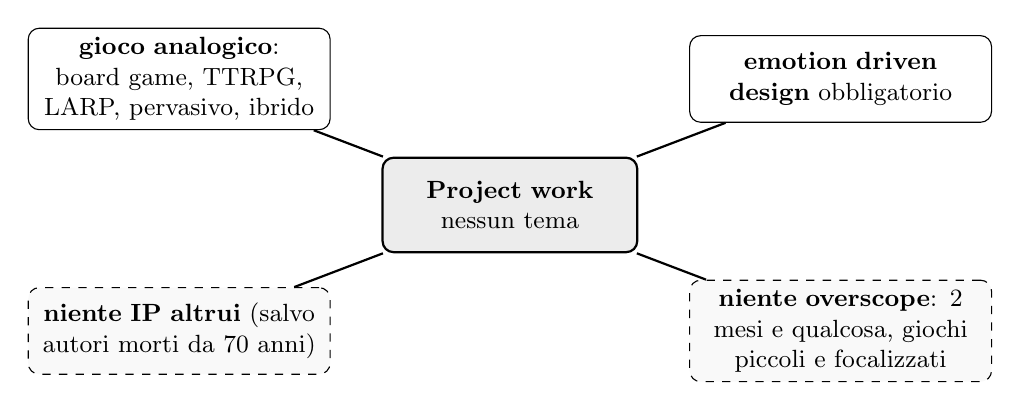
\begin{tikzpicture}[
    font=\small,
    centro/.style={draw, thick, rounded corners, fill=gray!15, text width=3.0cm,
      align=center, minimum height=1.2cm},
    vincolo/.style={draw, rounded corners, text width=3.6cm, align=center,
      minimum height=1.1cm, fill=white},
    no/.style={draw, dashed, rounded corners, text width=3.6cm, align=center,
      minimum height=1.1cm, fill=gray!5},
    linea/.style={thick}
  ]
  \node[centro] (c) at (0,0) {\textbf{Project work}\\ nessun tema};
  \node[vincolo] (a) at (-4.2,1.6) {\textbf{gioco analogico}: board game, TTRPG,
    LARP, pervasivo, ibrido};
  \node[vincolo] (b) at (4.2,1.6) {\textbf{emotion driven design}
    obbligatorio};
  \node[no] (d) at (-4.2,-1.6) {\textbf{niente IP altrui} (salvo autori morti da
    70 anni)};
  \node[no] (e) at (4.2,-1.6) {\textbf{niente overscope}: 2 mesi e qualcosa,
    giochi piccoli e focalizzati};
  \foreach \x in {a,b,d,e} { \draw[linea] (c) -- (\x); }
\end{tikzpicture}
\caption{Il \emph{mandate} del project work: due cose da fare (in alto) e due da
non fare (in basso, tratteggiate). Ricostruzione schematica della slide di
Daniele.}
\label{a7:fig:mandate}
\end{figure}

% ---------------------------------------------------------------------
\section{I gruppi}
\label{a7:sec:gruppi}

Poi i gruppi, tre gruppi da tre (tabella~\ref{a7:tab:gruppi}). La scelta è dei
docenti ed è ``insindacabile'', ma è basata sulle attività e sui task fatti
finora, ``sulla base di quello che vi abbiamo fatto fare negli ultimi giorni, come
lezioni, sulla vostra task e su quello che è stato un po' il nostro modo di
vedere''. Si è cercato di bilanciare anche gli \textbf{impegni di lavoro} di
ciascuno.

\begin{table}[htbp]
\centering
\begin{tabular}{@{}ll@{}}
\toprule
\textbf{Gruppo} & \textbf{Componenti} \\
\midrule
Gruppo 1 & Giordano, Nicola, Rita \\
Gruppo 2 & Gianmarco, Tancredi, Lorenzo Vergata \\
Gruppo 3 & Tiziana, Angelo, l'altro Lorenzo \\
\bottomrule
\end{tabular}
\caption{I gruppi del project work come li annuncia Daniele\protect\footnotemark.}
\label{a7:tab:gruppi}
\end{table}
\footnotetext{La trascrizione dice ``Giordano, Nicole, Rita, gruppo 2 Gianmarco,
Tancredi e Lorenzo V, gruppo 3 Tiziana, Angelo e Lorenzo''. ``Lorenzo V'' è Lorenzo
Vergata, come confermano poi i messaggi tra lui e Tancredi durante la pausa;
``Nicole'' è Nicola, a cui più tardi Beatrice dice che è nel gruppo ``con Giordano e
Rita''.}

Il progetto va sviluppato \textbf{durante il corso}: ``non vanno bene idee
pregresse, non portate nei vostri gruppi idee precedenti''. Le idee si sviluppano
insieme agli altri.

% ---------------------------------------------------------------------
\section{Le regole per lavorare in gruppo}
\label{a7:sec:regole}

Prima di lasciare la lezione a Beatrice, Daniele dà ``altri consigli per gli
acquisti''.

\paragraph{Rispettarsi.} ``La maggior parte del lavoro di un gruppo di sviluppo è di
\textbf{soft skill} più che di skill''. Bisogna capire come collaborare: se qualcuno
ha impegni di lavoro e fa fatica a garantire del tempo, ``partite da quello''. Non
si parte con ``un progetto grande come un castello disneyano'' per poi trovarsi
senza tempo; ci si dice invece ``io posso lavorare solo in questi momenti, lui o lei
solo in questi momenti'', e si cerca di fare ``qualcosa che abbia senso fare per il
tempo che abbiamo a disposizione''.

\paragraph{Taggare i docenti.} In caso di problemi si scrive ai docenti su
\textbf{Discord}, ma \textbf{taggandoli}: ``non lasciate messaggi senza taggarci,
se no li vedo una settimana dopo''. Oppure su \textbf{Telegram}.

\paragraph{Usare subito questi giorni.} Questi giorni vanno usati per il
\emph{brainstorming}: il tutoraggio con Ruggero è a breve (Daniele parla di ``48
ore'' per impostare il lavoro e capire che cosa fare).

\paragraph{Lavorare nel Drive.} Questa è una regola \textbf{obbligatoria}. Nel
Drive condiviso del corso ci sono le cartelle ``attività in classe'', ``dispense'',
``materiali didattici'' e ``project work''; dentro ``project work'' Daniele crea
tre cartelle, \textbf{gruppo 1}, \textbf{gruppo 2} e \textbf{gruppo 3}. Lavorare nel
Drive vuol dire evitare il più possibile di creare file fuori e caricarli dopo:
si aprono i Google Document lì e si lavora \textbf{in cloud}. Il motivo: se un
gruppo ha problemi e Daniele vuole aiutarlo, ha bisogno di vedere il
\textbf{processo mentale}, cioè che cosa è stato fatto nel documento, ``lo
\textbf{storico} del documento''. Un PDF o un \texttt{.docx} caricati così come
sono non hanno storico. Le cartelle vanno organizzate al meglio possibile; per
qualsiasi problema, ``basta chiedere''.

\paragraph{La dispensa sul brainstorming.} A seguito di questa lezione, ``tra stasera
e domani mattina'', Daniele registrerà una \textbf{dispensa}: il pezzo che venerdì
non c'è stato modo di fare, sul \emph{brainstorming} e sulla ricerca e sviluppo
``lato marketing'' e sugli strumenti di marketing nella ricerca e sviluppo. Metterà
a disposizione le slide e un video, con le slide del \textbf{brainstorming
strutturato}.

Nessuna domanda (``molti pollicioni, va bene''). Daniele ringrazia Bea ``per il
supporto e la condivisione'', saluta (``ci vediamo sicuramente il 12 di
ottobre'') e lascia la lezione.

% ---------------------------------------------------------------------
\section{Perché facciamo game design: due obiettivi}
\label{a7:sec:obiettivi}

``Ciao gruppo''. Beatrice comincia dando un po' di contesto: il corso è alla
\textbf{seconda edizione}, ci sono cambiamenti rispetto alla prima, e i docenti
stanno cercando di capire ``come rendervi il lavoro più agile e fattibile
possibile''. Nelle slide di oggi c'è molto, ``sarò onesta, credo troppo per la
lezione di oggi'', e quello che non si farà si riprenderà nella lezione successiva.
Il programma: ``mettere le mani in pasta'' per prepararsi ad affrontare un lavoro di
design; un po' di \emph{brainstorming} (da approfondire con i materiali di Daniele);
e una sorta di percorso di creazione di un gioco con un piccolo \textbf{esercizio di
design sprint}, a cui sarà dedicata la maggior parte della lezione. Alla fine del
corso i docenti chiederanno anche dei \textbf{feedback} su come è andato tutto.

Prima, però, un ``cappellino introduttivo'' sul \textbf{perché facciamo design}, già
anticipato nelle lezioni precedenti. Ci sono \textbf{due entità} che in questo
contesto si chiamano \textbf{obiettivi di design}:
\begin{enumerate}
  \item l'\textbf{obiettivo del gioco}, della produzione che si fa;
  \item l'\textbf{obiettivo personale} di chi progetta.
\end{enumerate}

\paragraph{L'obiettivo del gioco.} Un obiettivo di design del gioco, o del momento in
cui si sta facendo design, ha molte possibilità: raccontare un'esperienza di vita,
esplorare meccaniche o dinamiche, e così via; gli esempi della slide sono ``buttati
lì, sempre in brainstorming''. Si può decidere di fare un gioco per $N$ motivi, alcuni
personali e altri esterni al proprio bisogno personale.

Il punto è che \textbf{il motivo per cui affrontiamo la creazione di un gioco cambia
anche come progettiamo}. Beatrice vuole invitare la classe a ragionare su queste
cose, che spesso restano \textbf{ragionamenti interni} e invece è importante che
siano anche \textbf{condivisi}.

\paragraph{L'obiettivo personale.} L'obiettivo personale è semplice: rispondere alla
domanda \textbf{``perché sto facendo questo gioco?''}. Beatrice propone
\textbf{quattro categorie}, ``ma ce ne sono molte altre'', e probabilmente ne
emergeranno di nuove col crescere della disciplina; per la classe, i macro-obiettivi
saranno verosimilmente questi (figura~\ref{a7:fig:obiettivi}).
\begin{enumerate}
  \item \textbf{Voglio pubblicare un gioco.} Come gruppo di lavoro o come persona,
        voglio parlare a degli editori e pubblicare. Sotto questo cappello stanno sia
        la \textbf{pubblicazione con un editore} sia
        l'\textbf{auto\-pubblicazione}.
  \item \textbf{Voglio esprimere me stesso o me stessa.} È ``molto sottovalutato,
        troppo sottovalutato'': il gioco è uno strumento di espressione molto grande,
        che coinvolge anche altre persone. Magari non si vuole pubblicare né vendere,
        ma trasmettere davvero qualcosa che si è vissuto, qualcosa che si vuole
        raccontare; o si fa attivismo politico e si vuole un'attività che
        sensibilizzi sull'ecologia o su altri temi.
  \item \textbf{Voglio formare, informare o sensibilizzare.} Può sovrapporsi al
        punto precedente. Un gioco per insegnare meglio la matematica, per far
        conoscere un quartiere della propria città o un evento storico, per far
        crescere una competenza (aiutare le persone a parlare meglio in gruppo):
        ``$N$ situazioni di formazione''.
  \item \textbf{Voglio usare i giochi per il marketing e la comunicazione.} Portare
        l'attenzione su qualcosa: può essere un'espressione personale o una
        sensibilizzazione, ma anche un \textbf{prodotto} o un \textbf{servizio}. Lo si
        è visto con gli \emph{alternate reality game} del marketing, e in tante altre
        situazioni.
\end{enumerate}

\begin{figure}[htbp]
\centering
\begin{tikzpicture}[
    font=\small,
    domanda/.style={draw, thick, ellipse, fill=gray!15, text width=3.2cm,
      align=center, inner sep=2pt},
    ob/.style={draw, rounded corners, text width=3.3cm, align=center,
      minimum height=1.5cm, fill=white},
    freccia/.style={-{Stealth[length=2mm]}, thick}
  ]
  \node[domanda] (q) at (0,0) {\textbf{Perché sto facendo questo gioco?}};
  \node[ob] (p) at (-4.4,1.9) {\textbf{pubblicare}\\ con un editore o in
    autoproduzione};
  \node[ob] (e) at (4.4,1.9) {\textbf{esprimere me stesso/a}\\ raccontare,
    sperimentare, attivismo};
  \node[ob] (f) at (-4.4,-1.9) {\textbf{formare, informare, sensibilizzare}\\
    scuole, terzo settore, aziende};
  \node[ob] (m) at (4.4,-1.9) {\textbf{marketing e comunicazione}\\ prodotti,
    servizi, ARG};
  \foreach \x in {p,e,f,m} { \draw[freccia] (q) -- (\x); }
\end{tikzpicture}
\caption{Le quattro categorie di obiettivo personale proposte da Beatrice. ``Ce
ne sono molte altre''; esprimersi e sensibilizzare spesso si sovrappongono, e uno
stesso gioco può rispondere a più obiettivi.}
\label{a7:fig:obiettivi}
\end{figure}

% ---------------------------------------------------------------------
\section{Le competenze che ogni obiettivo richiede}
\label{a7:sec:competenze}

Ognuno di questi obiettivi personali richiede delle \textbf{competenze}, che ci si
fa ``in corso d'opera''. I docenti non si aspettano che gli studenti approfondiscano
ogni slide durante il corso, ma vogliono dire una cosa: se si crea un gioco, tutta
l'analisi di cui si è parlato (del mercato, delle persone, del target) va tenuta in
considerazione \textbf{in funzione dell'obiettivo}. Ogni obiettivo ha un modo
diverso di guardare il gioco e di produrlo. La slide mostra una ``carrellata'' di
competenze e conoscenze (tabella~\ref{a7:tab:competenze}).

\paragraph{Pubblicare con un editore.} Sono emerse domande anche dalla classe su come
capire che cosa sia meglio fare. Bisogna \textbf{conoscere il mondo della produzione}
di giochi da tavolo, di giochi di ruolo e di eventi ludici: chi esiste, che cosa fa,
a che prezzi mette fuori le cose, che tipo di prodotti vende già; se ci si riesce,
quante copie vengono vendute, quante persone comprano un biglietto. E
\textbf{conoscere le persone}: non solo ``c'è la casa editrice con il nome X'', ma
``all'interno ci lavorano X, Y, Z''. Partecipare agli eventi, mettersi in
connessione: sono tutte competenze, orientate a capire \textbf{come inserirsi} nelle
realtà che possono avere interesse a pubblicare.

\paragraph{Autoprodursi.} Le logiche sono diverse. Il mondo editoriale va conosciuto
comunque, perché in questo caso sono \textbf{competitor}; ma bisogna ragionare di più
verso il \textbf{pubblico}: capire come arrivare al momento in cui le persone
acquistano. Quindi parlare con gli utenti, affinare il marketing, analizzare i
competitor. E i competitor non sono solo quelli che fanno la stessa attività: per un
\textbf{evento dal vivo} un competitor può essere una fiera o un concerto, non per
forza un'attività di gioco; per un \textbf{gioco da tavolo formativo} un competitor
può essere un \textbf{corso}, non per forza un altro gioco. ``Immaginate i
competitor un po' più ad ampio spettro''. Infine, tutta una serie di informazioni
``non scontate'' e ``spesso prese sotto gamba'': \textbf{fiscalità e normative}.

\paragraph{Il GDPR: un'anticipazione.} Su questo, nella prossima lezione, Beatrice
farà ``un piccolo cappello'' sulle basi del \textbf{GDPR}, per poter raccogliere i
dati degli utenti e ricontattarli. È utile qualunque sia l'obiettivo: è sempre utile
avere, in una forma che permetta di risentirle, i dati delle persone con cui si è
venuti in contatto, che magari hanno testato il gioco, per tornare a scrivergli e
capire una serie di cose.

\paragraph{Esprimere se stessi.} Per sperimentare, per esplorare: qui ci sono
competenze ``spesso non raccontate, perché meno orientate al mercato'', che
riguardano \textbf{come trasmettiamo i contenuti} che vogliamo portare. È il lavoro
di \textbf{emotional design}, che ``sembra complicatissimo'', o comunque difficile da
definire; lo è, perché cambia per ogni gioco, ma col tempo si raffina sempre di più.
Chi vuole usare il gioco come sperimentazione personale, come linguaggio di dialogo
personale, deve capire bene quali sono i propri obiettivi: può essere ``voglio
comunicare la mia storia personale'', ma anche ``voglio trovare persone a me
affini'', o, ``banalmente'', ``voglio essere la persona che ha fatto il gioco più
conosciuto sulle \textbf{lumache da prato}''. Se è quello che si vuole raggiungere,
va bene: capito bene l'obiettivo, si capisce meglio tutto il resto, cioè
\textbf{che cosa voglio dire, a chi dirlo e perché} voglio dire determinate cose.

\paragraph{Formare, informare, sensibilizzare.} ``C'è un mondo'' su come si fa questo
design; qualcosa si vedrà nella prossima lezione, con le \textbf{escape room} e le
escape room formative. Per capire il mercato che può pagare queste attività, secondo
l'esperienza di Beatrice (``che non è onnisciente, ma è abbastanza puntuale al giorno
d'oggi''), le macro-voci in cui ci sono dei soldi, escludendo
l'\textbf{autofinanziamento} (che lei mette in una voce a sé), sono tre:
\begin{itemize}
  \item il \textbf{terzo settore} e i \textbf{bandi};
  \item il mondo delle \textbf{scuole} e della \textbf{formazione};
  \item la \textbf{formazione aziendale}: \emph{learning and development}, risorse
        umane e simili.
\end{itemize}
Sono tre mondi con logiche ``completamente diverse'' da quelle viste prima, e
Beatrice non ci si sofferma, perché non è il fulcro del corso. Ma già queste voci
bastano per sapere dove approfondire, se si vuole fare un gioco formativo: che cos'è
il terzo settore e che cosa significa proporgli dei giochi; che cosa sono i bandi
pubblici e quali enti li finanziano; e lo stesso per le scuole e per le aziende. E
poi c'è ``il magico mondo della \textbf{formazione finanziata}'', che sta sempre
sotto il cappello delle risorse umane: già googlando queste due parole si trovano
molte situazioni in cui si inserisce la proposta di giochi.

\paragraph{Il marketing.} Qui la parte principale da sapere è quella già vista
sull'\textbf{analisi del target} e sull'individuazione delle persone da coinvolgere.
Beatrice non si sofferma, perché secondo lei il marketing ``arriva dopo'': quando si
è progettato un po' di più (vale anche per la formazione) e si è sperimentato quello
che si è in grado di fare, allora si possono immaginare giochi per il marketing, che
sono giochi che portano l'utente a fare determinate cose. Per chi vuole approfondire,
la cosa principale è questa: si parla con delle \textbf{aziende}, e le aziende,
``anche le più virtuose'', hanno l'obiettivo di ``fare dei soldini''. Bisogna saper
rispondere alla domanda \textbf{``come aiuta l'azienda a fare più soldi?''}. I casi
sono due: \textbf{aumenta le vendite}, oppure fa aumentare \textbf{quanto l'azienda è
conosciuta}, o, se è conosciuta male, ne modifica in positivo la
\textbf{reputazione}. ``Non è un mondo bellissimo, ma è un mondo che esiste'': giochi
di questo tipo esistono tantissimo, e spesso non sono neanche raccontati come tali.
Beatrice lo dice perché magari si ha ``il gioco migliore del mondo'' e non si sa come
pagarsene lo sviluppo: questo può essere un modo.

\begin{table}[htbp]
\centering
\begin{tabular}{@{}p{3.0cm}p{9.6cm}@{}}
\toprule
\textbf{Obiettivo} & \textbf{Che cosa bisogna conoscere} \\
\midrule
Pubblicare con un editore & il mondo della produzione (chi c'è, che cosa fa, a che
prezzi, quanto vende); le persone dentro le case editrici; eventi e contatti \\
Autoprodursi & il mondo editoriale come competitor; il pubblico; marketing;
competitor ``ad ampio spettro'' (una fiera, un concerto, un corso); fiscalità e
normative; GDPR \\
Esprimere se stessi & come trasmettere i contenuti; \emph{emotional design}; che
cosa voglio dire, a chi e perché \\
Formare e sensibilizzare & terzo settore e bandi; scuole e formazione; formazione
aziendale (\emph{learning and development}, risorse umane); formazione finanziata \\
Marketing & analisi del target; ``come aiuta l'azienda a fare più soldi?'':
vendite, notorietà, reputazione \\
\bottomrule
\end{tabular}
\caption{Le competenze per obiettivo personale, ricostruite dalla carrellata di
Beatrice.}
\label{a7:tab:competenze}
\end{table}

\paragraph{Lo stesso gioco, più obiettivi.} Uno stesso gioco può rispondere a più
obiettivi. Si fa un gioco formativo, o un gioco per esprimersi, e si scopre che
potrebbe essere venduto a un'azienda, rispondere a un bando, entrare
perfettamente nel catalogo di un editore estero ``che non conoscevate fino a ieri'',
o di un editore italiano conosciuto in fiera. Quello che interessa a Beatrice è che
gli studenti abbiano chiari \textbf{gli interessi del mondo a cui parlano}, quando
hanno un gioco in progettazione o già fatto. Se si è consapevoli degli interessi
degli altri e del proprio obiettivo personale, ``diventa molto più facile il
dialogo''. Riuscire poi a vendere e ``imbroccare le cose giuste'' è un altro tema;
ma questi due elementi vanno avuti \textbf{prima}.

\paragraph{Approfondimento: il perché del designer.} Il tema dell'obiettivo personale
ha un parallelo in \emph{The Art of Game Design} di Jesse Schell, che apre il libro
non dal gioco ma dal designer stesso (``in the beginning, there is the designer''),
e più avanti dedica capitoli interi al rapporto con il \emph{cliente} e al
\emph{pitch}, cioè proprio al ``dialogo'' con gli interessi altrui di cui parla
Beatrice. Nella lezione, però, la distinzione tra
\emph{obiettivo del gioco} e \emph{obiettivo personale} ha soprattutto una funzione
pratica: è il primo argomento della chiacchierata iniziale del design sprint.

% ---------------------------------------------------------------------
\section{Il design sprint}
\label{a7:sec:sprint}

``Ora sono andata un po' veloce, e sono comunque lenta rispetto agli orari'':
Beatrice passa all'esercizio. Condivide un altro file (``che voi vedete bruttarello
qui e che poi vi caricherò''); chi non lo legge può mandarle ``un'emoji triste o
buffa''. Ha preparato \textbf{due moduli}; quello di adesso è su \textbf{come fare una
sessione di design sprint}.

\paragraph{Che cos'è.} Il design sprint si può usare per $N$ cose: ``dal decidere
come arredare casa a come risolvere il problema di non avere abbastanza soldi per
fare la spesa'', per qualunque problema. \textbf{Non è uno strumento nato per il game
design}: è nato per ragionare su problemi di progettazione e cercare soluzioni di
design. Beatrice lo ha \textbf{adattato all'uso sui giochi}, e lo ha diviso in
\textbf{fasi}, perché sono le fasi che invita i gruppi a provare a seguire. Il file
verrà caricato nella cartella condivisa degli strumenti. Oggi racconterà la prima
fase, ma la salterà, e si partirà dalla seconda.

\paragraph{Un invito, non un obbligo.} È ``uno strumento in più che vi dà una
direzione in caso la direzione non riusciate a trovarla in breve tempo''. Beatrice lo
dice apertamente: l'anno scorso alcuni gruppi hanno investito molto tempo in alcune
fasi della progettazione e non sono riusciti a concludere il gioco. Quest'anno si
vuole evitarlo, e per questo ci sono \textbf{due strumenti}: questo, e quello che si
vedrà alla fine di questa lezione e all'inizio della prossima, cioè tutte le voci che
compongono la progettazione di un gioco, per avere una \textbf{visione d'insieme} e
poter dire: ``abbiamo queste settimane prima del pitch e questi mesi prima della
consegna''. Ognuno ha un lavoro, una famiglia, dorme, mangia, fa cose che occupano
tempo: bisogna farsi ``dei conti pratici'', un tot di ore per una parte e un tot per
un'altra.

\paragraph{Il project management che non c'è.} Tutto questo fa parte del
\textbf{project management} di un progetto, e Beatrice avverte che nel mondo del
lavoro, ``nel gaming perlomeno'', \textbf{non esiste}: nella slide in cui sono state
presentate tutte le professioni non c'è un \emph{project manager} dei giochi, perché
le aziende sono ``ancora un po' in costruzione'' su questo lato; quelle italiane
almeno, mentre all'estero ci sono casi molto diversi, e nel videogioco funziona in un
altro modo. Questi strumenti vanno conosciuti per essere più consapevoli di
\textbf{come si funziona come persone}, preparandosi al fatto che il mondo esterno
non sempre segue logiche di organizzazione e ``più spesso bisogna un po' navigare le
onde''. Per il corso, però, sono molto utili: quando il gruppo ``per un attimo si
perde'', si può tornare a fare il punto con questi strumenti.

\subsection{Le fasi del file}
\label{a7:sec:fasi-file}

Beatrice scorre i ``titoloni'' del documento (figura~\ref{a7:fig:sprint}).
\begin{enumerate}
  \item \textbf{La chiacchierata iniziale}, che oggi si salta (si veda sotto).
  \item \textbf{Definire l'obiettivo di gruppo} del gioco: proposte e votazioni.
  \item Una piccola sessione di \textbf{ricerca e sviluppo} basata sull'obiettivo.
  \item Una prima sessione di \textbf{brainstorming} su quello che emerge, per
        rispondere all'obiettivo.
  \item La \textbf{valutazione} di tutto il brainstorming: che cosa si tiene e che
        cosa si butta, di tutte le idee uscite.
  \item Da lì in poi, l'\textbf{assegnazione dei ruoli}: chi fa cosa, con che tempi.
\end{enumerate}
Oggi si faranno le fasi dalla seconda in poi, fingendo che la classe sia un unico
grande gruppo di \textbf{nove persone} che inventa un gioco: ``faremo tutto quello
che serve per fare un brainstorming per avere il pitch del gioco''. Sarà un gioco
``del gruppo tutto'', quindi non lo si potrà portare a conclusione nel corso: serve
ad allenarsi con lo strumento.

\begin{figure}[htbp]
\centering
\begin{tikzpicture}[
    font=\small,
    fase/.style={draw, thick, rounded corners, text width=2.5cm, align=center,
      minimum height=1.3cm, fill=white},
    oggi/.style={fase, fill=gray!15},
    saltata/.style={fase, dashed, fill=gray!4},
    freccia/.style={-{Stealth[length=2mm]}, thick},
    nota/.style={font=\scriptsize\itshape, text width=2.5cm, align=center}
  ]
  \node[saltata] (f0) at (0,0) {chiacchierata iniziale (30 min)};
  \node[oggi, right=0.5cm of f0] (f1) {obiettivo del gioco: post-it e voto};
  \node[oggi, right=0.5cm of f1] (f2) {ricerca e sviluppo};
  \node[oggi, right=0.5cm of f2] (f3) {brainstorming su meccaniche, tipo,
    narrazione, setting};
  \node[oggi, below=1.1cm of f3] (f4) {voto, poi mappa impatto-sforzo};
  \node[oggi, left=0.5cm of f4] (f5) {percorso dell'utente};
  \node[fase, left=0.5cm of f5] (f6) {chi fa cosa, con che tempi};
  \node[fase, left=0.5cm of f6] (f7) {progettazione e sviluppo};
  \draw[freccia] (f0) -- (f1);
  \draw[freccia] (f1) -- (f2);
  \draw[freccia] (f2) -- (f3);
  \draw[freccia] (f3) -- (f4);
  \draw[freccia] (f4) -- (f5);
  \draw[freccia] (f5) -- (f6);
  \draw[freccia] (f6) -- (f7);
  \draw[freccia, dashed] (f7.north) -- node[midway, right=2pt,
    font=\scriptsize, align=left] {quando ci si perde:\\ di nuovo al voto}
    (f1.south west);
  \node[nota, above=0.1cm of f0] {saltata a lezione};
\end{tikzpicture}
\caption{Le fasi del design sprint adattato da Beatrice per il corso. In grigio le
fasi toccate a lezione (alcune solo raccontate per mancanza di tempo); la
chiacchierata iniziale è saltata. La freccia tratteggiata riassume il consiglio
``quando vi perdete, andate a votazione''. Ricostruzione schematica del file.}
\label{a7:fig:sprint}
\end{figure}

\paragraph{Una scaletta per il corso, non il design sprint.} Beatrice lo ripeterà più
avanti, a Nicola: la scaletta \textbf{non è una fase standard}, ``non voglio che vi
portiate a casa che il design sprint è tutto così, sempre, a queste fasi''. Prende
delle metodologie e le porta in una scaletta pensata per il corso.

\subsection{La chiacchierata iniziale}
\label{a7:sec:chiacchierata}

La prima fase è un \textbf{allineamento di gruppo}, e oggi si salta. Le domande:
\begin{itemize}
  \item quali sono i nostri \textbf{obiettivi personali} (quelli visti prima)?
        ``Magari il mio obiettivo in questo corso è provare a sperimentare. Oppure
        Lorenzo vuole fare un gioco per provare a venderlo da qualche parte, oppure
        io voglio fare un gioco per raccontare la storia della mia famiglia''.
        Allinearsi non vuol dire che sarà quello che si porterà a casa, ma che si
        conoscono i desiderata degli altri e c'è uno spazio per raccontare i propri;
  \item \textbf{che competenze ho}? A quali progetti ho già lavorato, e che cosa
        facevo in quei progetti?
  \item la ``domandona'': in questo corso voglio lavorare sulle \textbf{stesse
        competenze} su cui ho lavorato in passato, o ci sono attività che non ho
        ancora esplorato, che non ho mai fatto e vorrei esplorare qui? ``Non ho mai
        scritto testi, ma qua mi andrebbe di provare'', ``non ho mai fatto
        illustrazioni e qua mi andrebbe di vedere'': qui si può fare, e conviene
        capire in che ruolo mettere le proprie competenze. (Beatrice corregge anche
        un refuso nel file, in diretta.)
\end{itemize}
Per gruppi di tre persone, \textbf{30 minuti} bastano e avanzano: uno scambio in cui
``ognuno sa la situazione delle altre persone''. Beatrice invita a farla quando
inizierà il lavoro di gruppo.

\paragraph{Approfondimento: lo Sprint di Google Ventures.} Il \emph{design sprint}
nella forma più nota è quello descritto da Jake Knapp, con John Zeratsky e Braden
Kowitz, nel libro \emph{Sprint} (2016), nato a Google Ventures: cinque giorni per
passare da un problema a un prototipo testato con utenti reali, con passaggi molto
simili a quelli della lezione (mappare il problema, raccogliere ispirazioni,
proporre soluzioni individualmente e in silenzio, votare con adesivi a pallino,
decidere). L'adattamento di Beatrice ne conserva il cuore (lavoro individuale
silenzioso, presentazione, voto a pallini, tempi rigidi) ma lo piega ai tempi e agli
scopi di un corso: niente giornate intere, e la prima fase dedicata alle persone del
gruppo, non al problema.

% ---------------------------------------------------------------------
\section{La lavagna di Canva}
\label{a7:sec:canva}

``Ora vi condivido questa fantastica lavagna''. Per il \emph{brainstorming} ci sono
``tantissimi'' strumenti e modalità; oggi si usa il design sprint come modalità e una
\textbf{lavagna di Canva} come strumento.

\paragraph{Entrare.} Il link nella chat non è cliccabile, né si riesce a copiarlo
(``nemmeno copia e incolla''). Qualcuno lo copia a mano nella barra del browser e
riesce a entrare; un altro lo mette su Discord, dove ``funziona'', anche se a qualcuno
risulta che dal link di Discord non ha l'autorizzazione (``essendo che il link l'ho
copiato io, magari non ci sono i permessi''). Alla fine Beatrice crea un link
accorciato, ``più dettabile'' (\texttt{urli.it/31GRXQ}, secondo la trascrizione).

\paragraph{Gli strumenti in generale.} Canva è uno strumento per sessioni di
\emph{brainstorming} simile a molti altri; un altro è \textbf{Miro}, ``ma ce ne sono
davvero tanti''. Beatrice usa Canva perché è il più comodo per lei. L'impostazione
della lavagna \textbf{simula un incontro dal vivo}: le attività di oggi si possono
fare in digitale, a distanza, con uno strumento di questo tipo, oppure dal vivo con
\textbf{carta e penna}, un tavolo dove appoggiare i bigliettini, un muro dove
attaccare i post-it. ``Ve lo dico perché può essere utile anche per il futuro''.

\paragraph{Come si usa.} Beatrice ha ``loccato'' (bloccato) gli elementi della
lavagna, così che nessuno sposti per errore le cornici; si può selezionare e
zoomare liberamente (avvicinandosi le lavagne ``diventano più grandi''), ma bisogna
stare attenti a non cancellare il lavoro degli altri. Per cancellare: si seleziona
l'elemento e si preme il tasto di cancellazione, oppure il piccolo cestino nel menu
dell'elemento. Gli strumenti utili sono nel \textbf{menu a sinistra} di Canva, che ha
sette voci (Canva AI, Modelli, Elementi, Testo, Brand, Caricamenti,
\textbf{Strumenti}); sotto \textbf{Strumenti} (l'icona con una ``pennina'') ci sono,
tra gli altri, il \textbf{testo} e i \textbf{foglietti adesivi}: ``veri e propri
post-it, come quelli che usereste dal vivo''. Si sceglie un colore, il post-it compare,
lo si ingrandisce o rimpicciolisce e ci si scrive sopra.

\paragraph{Le prove.} La prova serve anche ad allinearsi sullo strumento, ed è
movimentata. I post-it compaiono uno dopo l'altro (``Giordano, anche Lorenzo'',
``vedo una C'', ``Rita sta scrivendo''); Gianmarco entra senza il suo account e
compare come ``Leone Marino'', uno dei nomi di animale che lo strumento assegna
agli utenti anonimi\footnote{La trascrizione dice ``è come l'anonimo di Giuseppe'':
con ogni probabilità il riferimento è agli ``animali anonimi'' con cui Google e
altri servizi mostrano chi partecipa senza account.}. Si scopre che se la
lavagna di base è bloccata non si riesce a scrivere nei post-it (``io l'ho imparato
adesso, perché credevo non funzionasse così''), e Beatrice sblocca. Qualcuno sposta
per sbaglio l'intera cornice (``oh mio Dio, sono uscito, e qualcuno ha spostato tutta
la lavagna''), qualcuno ha post-it finiti fuori dalla lavagna o giganteschi, una
studentessa (``una grafica fissata con l'impaginazione'') prova a riallineare
tutto. Angelo, che è collegato \textbf{dal cellulare}, non riesce a trascinare il
post-it (``non me lo fa trascinare''); Beatrice lo guida passo per passo e alla fine
decide di creargli lei dei post-it con il proprio nome sopra, che Angelo userà
(``ci ricorderemo che i tuoi post-it sono quelli con il nome di Beatrice''), anche
se poco dopo Angelo riesce a crearne uno da solo (``ce l'ho fatta'').
``Dal telefono è anche più complicato, è normalissimo''. Beatrice avverte che
\textbf{Miro è un po' più intuitivo} di Canva, e che servirà molto spazio: il gioco di
fare le cose piccole e zoomare sarà utile soprattutto nella ricerca e sviluppo.

\paragraph{Lo strumento conta il giusto.} ``Di tutto questo, lo strumento ci interessa
il giusto'': si può usare Miro, si possono scrivere le cose a mano. \textbf{Ci
interessa il procedimento}.

% ---------------------------------------------------------------------
\section{Prima fase: che obiettivo vorrei dare a questo gioco?}
\label{a7:sec:fase1}

La domanda della prima fase è \textbf{``che obiettivo vorrei dare a questo
gioco?''}. Le regole:
\begin{itemize}
  \item ognuno scrive \textbf{al massimo tre risposte}, e almeno una;
  \item \textbf{una risposta per post-it};
  \item non è il genere del gioco e non sono le meccaniche: è ``più a volo
        d'aquila'', quello che si vorrebbe che il gioco ottenesse; può riguardare
        anche le \textbf{emozioni}, cioè che cosa far provare alla persona che gioca.
\end{itemize}
Gli esempi del file mescolano apposta livelli diversi: ``un gioco formativo per
insegnare l'inglese'', ``un gioco con dei pinguini blu'', ``un GDR per sensibilizzare
sulla lotta di classe'', ``un gioco fantasy sulla vendetta'', ``un gioco con delle
pedine gigantesche'', ``un gioco che faccia esplorare un quartiere''.

\paragraph{I timer.} E qui la cosa da ricordare di tutto il procedimento:
\textbf{mettere i timer}. Nei processi creativi di gruppo, e probabilmente lo si è già
visto succedere, ci si fa prendere da quello che sta avvenendo, dai dialoghi, dalle
idee che emergono. Beatrice richiama la lezione precedente su \textbf{divergenza e
convergenza}: c'è un momento in cui si apre, si esplora, si buttano idee; ma ``a un
certo punto bisogna \textbf{quagliare}''. Darsi un tempo di orologio dice fino a
quando si esplora; quando suona il timer, bisogna riportare in ordine la situazione.
``È la cosa importante di tutto il processo: dare dei tempi e provare a
rispettarli''. Il primo timer è di \textbf{5 minuti} (``dai 5 ai 10'').

\paragraph{Gianmarco arriva.} Gianmarco, ``arrivato un po' in corsa'', chiede il
contesto: si può buttare qualsiasi idea? È un esercizio, risponde Beatrice, per
imparare a fare \emph{brainstorming} e poi mettere in ordine le idee: ``vai pure
libero''.

\paragraph{La parola proibita.} Mentre scrivono, Rita avverte i compagni: qualcuno
ha scritto \emph{divertire} su un post-it, e ``dovremmo evitare di usare questo
verbo''\footnote{Il riferimento è alla regola, ricorrente nel corso, per cui ``far
divertire'' non è un obiettivo di design: è troppo generico per orientare le
scelte.}, ``conviene modificarlo prima che lo veda qualcuno'' (Ruggero, si
capisce). Beatrice: ``Io non dirò niente, però è un ottimo consiglio''. Del resto,
aggiunge, sono idee che non verranno condivise con gli altri docenti: è un esercizio
per imparare la procedura, che non è neanche detto si userà esattamente così. Le idee
di oggi possono avere vita propria e crescere, ``ma non in questo corso'': i gruppi
del progetto partiranno da zero.

% ---------------------------------------------------------------------
\section{Il racconto delle idee}
\label{a7:sec:racconto}

Prima della votazione, che Beatrice anticipa (si veda la
sezione~\ref{a7:sec:votazione}), \textbf{ognuno racconta che cosa ha scritto} e dice
\textbf{dove sono} i suoi post-it, così che tutti possano trovarli sulla lavagna. In
questa fase valgono due regole:
\begin{itemize}
  \item le altre persone possono fare \textbf{solo domande}: chiarimenti su che cosa
        si intende, su perché è emersa un'idea; ``tutte le domande che vi vengono in
        mente vanno benissimo'', anzi Beatrice invita a farle, perché ``c'è ancora
        tanto che può uscire'';
  \item \textbf{niente commenti}, ``né nient'altro''. Se non si hanno domande, non si
        dice nulla.
\end{itemize}
E Beatrice si fa da parte: ``fate finta che io non esista''. Ricorderà solo di dire
dove sono i post-it; il gruppo deve autogestirsi, come in un vero lavoro di gruppo
in cui nessuno dà la direzione. Poi si accorge di aver dimenticato il timer anche
qui: tutte le idee vanno raccontate in circa \textbf{15 minuti}, ``tenetene conto
quando fate le domande, quando rispondete, quando raccontate''.

\subsection{Rita}
\label{a7:sec:idee-rita}

Rita (post-it arancione, rosso e giallo, sovrapposti nell'angolo in alto a sinistra)
ha scritto tre idee.
\begin{description}
  \item[Un gioco educativo.] Si è avvicinata a questo mondo con l'idea di dare
        qualcosa in più alle nuove generazioni: è quello che l'ha spinta a diventare
        game designer.
  \item[Un gioco che costringe le persone a collaborare.] Quando la collaborazione è
        necessaria per raggiungere un obiettivo, bisogna affrontare problemi con se
        stessi e con gli altri, e questo è costruttivo e stimolante per tutti. È anche
        il suo approccio alla vita: ``condividere, collaborare per imparare''.
  \item[Un gioco sull'arte.] È la sua più grande passione: avvicinare le persone a
        un'arte ``non proiettata verso l'IA''.
\end{description}
Le domande. Il gioco sull'arte è sulla storia dell'arte, i grandi pittori, o un gioco
in cui \textbf{le persone fanno gli artisti}? La seconda: avvicinarle alla disciplina
in maniera attiva; e in effetti, osserva Rita, potrebbe rientrare nel gioco educativo,
con le scuole. Il gioco educativo, per che età e in che contesto? Non ci ha ancora
pensato nello specifico, ma pensava a bambini che stanno crescendo, elementari e
medie: per gli adolescenti ci vuole qualcosa di più attivo e stimolante a livello
emotivo, forse un LARP. Poi chiede lei un parere a una compagna con esperienza di
questi giochi: ci sono fasce d'età più interessate a certi tipi di gioco?
``Dipende'', risponde la compagna: si sente il gruppo, e se il gioco è educativo lo
si orienta anche, per esempio decidendo se farlo competitivo o no. A lei è sempre
piaciuto \textbf{mescolare competizione e collaborazione}: le \textbf{cacce al
tesoro} sono notoriamente competitive, ma le sue richiedevano sempre una
collaborazione tra i gruppi, e alla fine \textbf{il tesoro era per tutti}: c'era la
soddisfazione di chi era arrivato primo, ma il premio era di tutti. ``Bello, e
stimolante, perché si deve collaborare per raggiungere un obiettivo''.

\subsection{Nicola arriva}
\label{a7:sec:nicola}

A questo punto entra Nicola. Beatrice gli spiega in breve che cosa sta succedendo:
un esercizio di design sprint, ``una metodologia, anzi varie metodologie che
riguardano tante forme di design, non solo quello dei giochi'', per avere una
direzione quando un gruppo si perde o non sa come allinearsi; la prima fase è
rispondere a ``che obiettivo vogliamo dare al gioco''; i compagni hanno dato tre
idee ciascuno, che ora si leggono e poi si votano. E gli dice il suo gruppo: ``sei nel
gruppo 1, con Giordano e Rita'', ``non per motivi'', lo rivedrà nelle slide che
Daniele caricherà. Nicola entra nella lavagna come ``Nick''.

Poco dopo, Nicola chiede ``un quick check-up'': si sente ``in alto mare'', ``una
zavorra''. I post-it sono già divisi in gruppi? Sono concept di personaggio o di
gioco, di ogni singola persona? Si stanno comparando? Beatrice riconosce di non
essersi spiegata abbastanza e rispiega: si sta \textbf{testando la metodologia},
fingendo di essere un unico gruppo di nove da cui deve uscire ``una bozza di gioco'';
la scaletta non è standard ma costruita per il corso; per decidere l'obiettivo del
gioco ognuno butta giù idee in silenzio sui post-it, poi le si leggono (``una fase di
brainstorming aperto'') e infine le si vota.

Nicola chiede com'è il voto: qualitativo o quantitativo? Si vota sulla quantità di
contenuto, sulla tipologia, ``un voto vale più di un altro''? Nessun voto vale più di
un altro, risponde Beatrice: ognuno avrà \textbf{sei voti}, ``immagina di avere sei
pallini adesivi'', e può metterli anche tutti sulla stessa idea. A Nicola lo schema
ricorda quello studiato in \textbf{organizzazione aziendale}, quando si avvia un
progetto; Beatrice conferma che il design sprint si usa in moltissimi contesti, ``molto
sulle soluzioni da proporre'', anche in sociologia. Nicola chiede ancora se c'è stata
una spiegazione prima del lavoro: c'è stata una piccola introduzione sui motivi per cui
si fa design (recuperabile dalle slide o dalla registrazione), e poi ci si è buttati
sulla domanda. Infine: ci sono linee guida, ``o siamo randomici''? ``Per ora è tutto
libero, rimaniamo leggerissimi''. Nicola si scusa con la classe per il tempo rubato.

\subsection{Lorenzo Vergata}
\label{a7:sec:idee-vergata}

Lorenzo Vergata (post-it sopra quelli di Rita) presenta tre idee, mentre ``qualcuno
ha mosso la lavagna'' e per un momento ``è scomparso tutto''.
\begin{description}
  \item[I funghi.] \textbf{Esplorazione del bosco per sensibilizzare sulle specie
        fungine e sul rispetto della natura}, ``semplicemente perché siamo in periodo
        di funghi'': la prima cosa che gli è venuta in mente.
  \item[Frenetismo.] Partite rapide, ``quasi caotiche dall'esterno, ma
        pseudo-organizzate dall'interno fra i giocatori''. Si è chiesto che cosa cerca,
        a 26 anni, in un gioco: non partite lunghe, ma frenesia. Frenesia, quindi,
        ``per gente neolaureata e simile''.
  \item[Paura.] Nascondino; fuggire da qualcuno all'aperto, senza luci; o in casa,
        staccando la corrente all'inizio del gioco. ``Il gioco deve far paura'':
        senza aver fatto ricerca, pensa che non ci siano molti giochi che sfruttano la
        paura dei giocatori come dinamica.
\end{description}
Le domande, e qualche commento che sfugge alla regola. L'idea della paura è pensata
come un \textbf{LARP}, all'esterno, o come un gioco da tavolo? Lorenzo pensa che il
modo più semplice di creare paura sia un LARP, ma ``nulla toglie'' di farlo da tavolo,
studiando come un gioco da tavolo possa incutere timore. Una compagna osserva che la
paura si definisce in tanti modi: \textbf{pressione}, \textbf{ansia} (più facili da
tavolo) e \textbf{jumpscare} (più da LARP); bisognerebbe dare una dimensione al
concetto, ma è ``una bella sfida''. Le ricorda quando da ragazzina giocava a
\textbf{guardie e ladri} al mare, di notte, nelle case degli amici: si creava un
clima di paura e tensione, anche perché ci si facevano gli scherzi.

Un altro studente, che gioca ``per la maggior parte del tempo'' a giochi di ruolo da
tavolo\footnote{Dal contesto, con ogni probabilità Nicola, che poco dopo si presenta
come ``un grande giocatore di TTRPG''.}, conferma che la paura è ``un fantastico
strumento'', ma pone un problema: se diventa un \textbf{gioco pervasivo}, c'è un
\textbf{danno collaterale}, cioè \textbf{spaventare chi non gioca}. ``Immagino una
persona che corre a mezzanotte in giro per Roma urlando di paura'': terrificante per
chi la vede, e si coinvolgono persone che non vorrebbero provare quella paura.
Lorenzo concorda: bisognerebbe tarare, andando più verso quello che diceva la
compagna, cioè il momento in cui sei nascosto e senti che chi ti cerca è ``letteralmente
a fianco a te'', e ti pervadono paura e ansia. Ma ``basta poco'' per tirare in mezzo
estranei: chi vede una persona che ne insegue un'altra che cerca di nascondersi
``chiama la polizia al minuto zero''. Se sono bambini di sei anni, ``stanno
giocando''; se vedi un ventenne, ``che cosa sta accadendo?''.

Infine l'esplorazione del bosco: come sarebbe, come gioco? Una guida che ti porta nel
bosco? ``Fatta sul posto è tosta'': sarebbe semplicemente una gita con un
\textbf{micologo}. Ma \textbf{da tavolo} si potrebbe fare. Sul fronte della natura si
possono inserire meccaniche che \textbf{simulano il comportamento dei funghi}: sotto
di loro c'è il \textbf{micelio}, che fa da rete di comunicazione tra le piante, e ne
potrebbe uscire un gioco ``pseudostrategico''. Sulla \textbf{commestibilità} si può
immaginare uno scontro carta contro carta, una specie di sasso-carta-forbice: ``il
fungo buono te lo annullo con questo cattivo'', mentre certi funghi che ``sembrano
buoni'' rovinano tutto il raccolto, cioè una sola carta può rovinare molte carte di
funghi buoni. ``Potrebbe anche essere frenetico, chissà''.

\subsection{Tancredi}
\label{a7:sec:idee-tancredi}

Tancredi ha scritto in modo ``molto più riassunto''.
\begin{description}
  \item[Un gioco cooperativo.] È ``un grande fan dei cooperativi'', anche piccoli,
        come \emph{Hanabi}\footnote{La trascrizione dice ``Anabis''.}, \emph{Sky Team},
        \emph{Quicksand}: gli piace molto la meccanica della cooperazione.
  \item[Un gioco per il terzo settore.] Riprende la categoria vista prima, ma senza
        grandi idee: per questo tipo di gioco sarebbe importante capire \textbf{per chi}
        lo si fa, e non sa quanto sia realizzabile nel loro caso.
  \item[Un GDR.] Non conosce praticamente per niente i giochi di ruolo, li ha
        scoperti in queste lezioni: ``perché no?'', provare a sperimentare quel
        settore.
\end{description}
Che cosa aveva immaginato per il terzo settore? Secondo Tancredi un modo sarebbe
cercare delle realtà, anche solo su internet, sui loro siti, e capire che cosa
potrebbe essere interessante per loro, ``anche se poi non glielo si propone
veramente, perché questa è un'esercitazione''; con l'obiettivo di dare una mano,
diffondere quello che fanno. Un compagno racconta (più un commento che una domanda)
di aver giocato \emph{Nemesis: Retaliation} dal vivo nella modalità semicooperativa,
con i traditori, e ora online su \textbf{Board Game Arena}\footnote{La trascrizione
scrive ``BGA'', la sigla abituale del sito.} con più o meno gli stessi amici, in
modalità cooperativa, usando la chat: ``stratosferico, così mi diverto''. Se invece
``a un certo punto uno ti dà una ginocchiata sui denti''\ldots{} Tancredi: in
associazione ``quasi mai nessuno vuole fare cooperativi'', e lui è sempre lì; gli
piacciono anche i competitivi, ma certi giochi ``vale la pena giocarli così''.

\subsection{Tiziana}
\label{a7:sec:idee-tiziana}

Tiziana (post-it sotto quelli di Tancredi) ha scritto tre idee.
\begin{description}
  \item[Un board game, di costruzione, gestionale ambientato.] Le piacerebbe fare
        esperienza di costruzione di un gioco da tavolo e non saprebbe da che parte
        cominciare (come Tancredi con i giochi di ruolo: ``non ho idea, quindi mi
        piacerebbe provare''). Un \textbf{gestionale} perché le piace l'aspetto
        gestionale, ma \textbf{ambientato}, ``non so se è una chimera''.
  \item[Un'escape room per far divertire.] ``Lo so che non devo usare divertire, ma
        non sono riuscita a trovare nessun'altra cosa'', e soprattutto far divertire
        lei mentre la costruisce. E far nascere la \textbf{collaborazione}. Dal vivo o
        da tavolo, entrambi vanno bene; il tema non lo sa. Le piacciono gli
        \textbf{indovinelli}, trovare soluzioni; ma vorrebbe enigmi \textbf{misti}, non
        tutti dello stesso tipo, perché quando sono tutti uguali diventano ``o troppo
        cervellotici o ripetitivi''.
  \item[Un gioco interattivo per far conoscere la città.] Una parte di essa, perché
        Roma ``è abbastanza gigantesca''; l'aveva immaginato coinvolgendo perfino i
        \textbf{passanti}, ``ma non so se sia fattibile''.
\end{description}
Tancredi chiede: quando parli di gestionale, hai un riferimento? Un gioco economico,
con competizione e interazione molto alte, o qualcosa di meno interattivo,
``più German''? Tiziana non lo sa: da giocatrice è più ``mi coltivo il mio orticello''
(gli economici interattivi ``non sono i miei preferiti''), ma potrebbe essere anche
interattivo: intendeva la \textbf{gestione delle risorse} in generale. La cosa
fondamentale è che sia ambientato, ``che senti di essere in quel posto''. Un
compagno le suggerisce \emph{Akropolis}, per l'ambientazione e per l'idea di
costruire la propria città con tessere di tre esagoni sovrapposte, in cui i colori che
restano in cima diventano i quartieri: un approccio per non renderlo ``troppo
gestionale German'', magari con una città costruita tutti insieme. Tiziana non lo
conosce. Beatrice interviene: si possono fare domande, ``ma non altre cose'',
altrimenti si usa troppo tempo; e manca un minuto. Tancredi: ``domanda sbagliata,
scusate''. ``Va tutto bene, siamo qui apposta per capire le dinamiche''.

\paragraph{Il timer che scade.} Manca un minuto e mancano ancora cinque persone.
Beatrice concede \textbf{altri dieci minuti}, ``ma dentro questi dieci minuti dovete
starci'': alla fine si passa allo step successivo, ``quello che è stato detto è stato
detto''. Qualcuno propone due minuti a testa; ``se volete, sì, però non posso
dirvelo io'': serve ad allenare il gruppo.

\subsection{Angelo}
\label{a7:sec:idee-angelo}

Angelo, colto un po' di sorpresa (``ci ho messo un'eternità a scriverlo, abbiate
pazienza''), ha i post-it in basso a sinistra.
\begin{description}
  \item[Un gioco di ruolo basato su un'app.] Così che la \textbf{mappa} possa essere
        continuamente aggiornata.
  \item[Un board game con possibili espansioni.] Qualcosa ``tipo \emph{Magic}, ma non
        per forza così evoluto'': ogni tanto si aggiungono carte che modificano la
        strategia.
\end{description}
Il tema è variabile, ma più fantasy o fantascienza che realismo; non aveva pensato a
un'emozione particolare. Qualcuno trova interessante il board game ``aggiornabile''.
E che cosa intende per mondo condiviso? Qualcosa come i giochi online divisi per zone
(Europa dell'Est, Europa dell'Ovest), ma molto più ristretto: si parte con
un'avventura in un \emph{medieval fantasy}, e qualcuno nella tua zona pensa a un'isola
con ambientazione \emph{steampunk} e la aggiunge al mondo, così che altri possano
andarci e ``ruolare'' in un mondo steampunk. ``Una sorta di \emph{sandbox}'':
ognuno parte dal suo stile e ci si trova in posti sempre diversi, senza un paesaggio
ripetitivo.

\subsection{Gianmarco}
\label{a7:sec:idee-gianmarco}

Gianmarco (in basso a destra) presenta tre idee.
\begin{description}
  \item[Un gioco da tavolo per bambini dai 6 agli 8 anni.] Che li spinga a
        \textbf{raccontare}, incentrato su \textbf{esplorazione e scoperta}: è la fase in
        cui i bambini iniziano a staccarsi un po' dai genitori, e nell'esplorare provano
        ``quel misto di curiosità e paura''. Con elementi grafici, un po' di
        casualità; una parte di sistema per sviluppare la \textbf{logica} e una parte di
        immagini per l'\textbf{immaginazione}.
  \item[Un board game narrativo sulla guerra.] Con le meccaniche di \emph{Mage
        Knight}\footnote{La trascrizione dice ``Image Night'' e ``Mage Night''.}:
        ``l'ho veramente buttato a caso, è una cosa senza senso''.
  \item[Un'escape room basata sul tempo.] Si deve uscire dall'ufficio, ma il tempo
        non scorre mai: bisogna risolvere enigmi per far scattare \textbf{le 17} e
        uscire finalmente.
\end{description}
Un compagno ricorda una scena dei \emph{Simpson} in cui Bart guarda continuamente
l'orologio della classe, che a un certo punto torna indietro; e suggerisce una
meccanica del tempo non in tempo reale ma a eventi, ``cose che si innescano dopo tot
minuti'' (``so che tra tre minuti mi bolle l'acqua e succede qualcosa''). Un altro
nota che è bella ``la cosa al rovescio'': di solito il timer si accorcia e ti
esaurisce, qui devi farlo andare avanti. Qualcuno trova curiosa l'idea centrale e
chiede perché le meccaniche di \emph{Mage Knight} dovrebbero rappresentare l'orrore
della guerra. Il motivo è semplice: è un periodo di guerra, a Gianmarco piace
\emph{Mage Knight} e gli piacciono i board game narrativi, ``ho messo tutto insieme,
ho fatto un po' un pastiche''.

\subsection{Nicola}
\label{a7:sec:idee-nicola}

Mancano tre minuti e mezzo per tre persone: ``un minuto a testa''. Nicola va
``rapidissimo''.
\begin{description}
  \item[Un gioco di ruolo sui tempi morti: la cucina.] È un grande giocatore di
        TTRPG, e ha notato che i giochi di ruolo da tavolo hanno regole ben stabilite
        ma quasi nessuno ha meccaniche sui \textbf{tempi morti}: in un fantasy alla
        \emph{D\&D}, quando ci si accampa ``è sempre molto randomico''. Gli
        interesserebbe un GDR basato sulla \textbf{cucina}: restare sazi per andare
        avanti nelle missioni, arrangiarsi con quello che si trova; ispirandosi a
        \emph{Dungeon Food}\footnote{Così nella trascrizione. Si tratta con ogni
        probabilità di \emph{Dungeon Meshi} (in italiano \emph{Dungeon Food}),
        manga e anime in cui gli avventurieri cucinano e mangiano i mostri del
        dungeon.}, dove si mangiano i mostri per andare avanti, perché non sempre si
        hanno le provviste.
  \item[Un gioco strategico con bluff e ruoli nascosti.] Da giocatore di ruolo, perché
        non provare uno strategico da tavolo? Lo baserebbe sulla deduzione, sul
        \textbf{bluff} e sui \textbf{ruoli nascosti}. Su una gigantesca plancia ognuno
        parte senza nazione e, ispirandosi al videogioco strategico \emph{Humankind},
        ne sblocca: Roma, che vince \textbf{conquistando}, e allora la tua strategia
        diventa conquistare; più avanti gli Egizi, che vincono \textbf{costruendo
        opere}. L'obiettivo è non far capire \textbf{in che modo vuoi vincere}: quale
        nazione, o quale somma di nazioni, sei, e quali sono i tuoi metodi di vittoria.
  \item[Un LARP sul cambiamento visibile dei personaggi.] Non ne sa niente, ma gli
        interessa: persone vestite di bianco, ``come dei camici bianchi'', senza
        emozioni. Chi si sporca di \textbf{rosso} diventa più nervoso, rabbioso,
        isterico; di \textbf{blu}, più triste; di rosso e blu, arrabbiato e triste;
        di \textbf{verde}, prova anche disgusto. Una \textbf{somma di emozioni}, con
        obiettivi che costringono a sporcarsi: ``devi prendere la chiave segreta dentro
        il secchio rosso; ora hai la mano e mezza manica sporche di rosso, sei anche
        rabbioso''.
\end{description}

\subsection{L'altro Lorenzo}
\label{a7:sec:idee-lorenzo}

L'altro Lorenzo non è sicuro di aver seguito bene l'obiettivo: forse è stato
``troppo personale, troppo generico''. Ha scritto: \textbf{esprimere me stesso};
\textbf{raccontare il mio mondo fantasy attraverso un GDR}; \textbf{esplorare
tipologie di gioco nuove}, almeno per lui, come l'escape room o il LARP. Non ha in
mente cose specifiche. Qualcuno gli chiede se ne aveva in mente parlando del suo
gioco: sì, ma era un pensiero personale, e in un lavoro di gruppo ``non è che si può
imporre per forza il proprio mondo scritto''.

\subsection{Giordano}
\label{a7:sec:idee-giordano}

Il timer è scaduto, ma Beatrice concede a Giordano, l'ultimo, una breve presentazione
(all'inizio non si sente). Giordano non ha puntato su un gioco specifico ma su
\textbf{aspetti da inserire} in un gioco. Il primo è l'\textbf{accessibilità}: ``non
vorrei che qualcuno potesse mai dire \emph{non posso giocare a questo gioco}; al
massimo, \emph{non mi interessa}''. Il secondo è la \textbf{creatività}: di chi gioca,
precisa a una domanda, non di chi progetta.

\begin{table}[htbp]
\centering
\small
\begin{tabular}{@{}p{2.3cm}p{10.4cm}@{}}
\toprule
\textbf{Chi} & \textbf{Le idee sui post-it} \\
\midrule
Rita & gioco educativo (elementari e medie); gioco che costringe a collaborare;
gioco sull'arte, in cui si fa gli artisti \\
Lorenzo Vergata & esplorazione del bosco per sensibilizzare sulle specie fungine e
sul rispetto della natura; frenesia (partite rapide, caotiche fuori e organizzate
dentro); paura (nascondino, fuga al buio) \\
Tancredi & gioco cooperativo; gioco per il terzo settore; GDR \\
Tiziana & board game gestionale ambientato; escape room con enigmi misti e
collaborazione; gioco interattivo per far conoscere una parte di Roma \\
Angelo & GDR con app e mappa condivisa aggiornabile; board game con espansioni che
cambiano la strategia \\
Gianmarco & gioco per bambini di 6--8 anni su esplorazione e scoperta; board game
narrativo sulla guerra con le meccaniche di \emph{Mage Knight}; escape room in cui
bisogna far arrivare le 17 \\
Nicola & GDR sulla cucina e i tempi morti; strategico con bluff e nazioni nascoste;
LARP delle emozioni a colori \\
l'altro Lorenzo & esprimere se stesso; il proprio mondo fantasy in un GDR; esplorare
escape room e LARP \\
Giordano & accessibilità; creatività di chi gioca \\
\bottomrule
\end{tabular}
\caption{Le idee della prima fase dell'esercizio, persona per persona.}
\label{a7:tab:idee}
\end{table}

% ---------------------------------------------------------------------
\section{La votazione a pallini}
\label{a7:sec:votazione}

Beatrice blocca la lavagna (i post-it non si possono più spostare, ma ci si può
scrivere sopra), allarga un po' lo spazio dei post-it di Rita, e spiega prima
l'attività in sé, poi come farla su Canva.

\paragraph{Le regole.} Ognuno ha \textbf{sei pallini}: ``immaginatevi proprio di avere
dei pallini adesivi''.
\begin{itemize}
  \item Si mettono sulle idee che piacciono di più, cioè quelle \textbf{che si
        vorrebbero produrre}, su cui si vorrebbe lavorare.
  \item Si possono mettere \textbf{più pallini sulla stessa idea}, anche tutti e sei.
  \item Si può \textbf{votare la propria idea}.
  \item \textbf{Non si deve spiegare} perché si vota.
  \item Si devono \textbf{usare tutti e sei}: non si può non votare o metterne meno.
\end{itemize}
Alla fine restano solo i post-it con più pallini. Se uno ne ha più degli altri, è
l'idea su cui si lavora; se ce ne sono due o tre in testa, \textbf{si rivota} tra
quelli.

\paragraph{Su Canva.} Beatrice propone, ``brainstormando sempre, quindi non so se è
l'idea migliore'', di usare i \textbf{pennarelli} di Canva (ancora in Strumenti),
ognuno con un colore. Seguono le prove fuori dalla lavagna (Beatrice disegna ``un
cuore gigantesco viola'') e un lungo appello dei colori, complicato dal fatto che il
colore del cursore di qualcuno non coincide con quello del suo pennarello e che
compaiono più ``soli'' disegnati per prova\footnote{L'assegnazione dei colori, per
quanto ricostruibile: Giordano arancione, Nicola verde chiaro, Lorenzo Vergata ``blu
pastello'', Tancredi blu, Gianmarco viola scuro, l'altro Lorenzo rosso, Tiziana nero,
Angelo azzurro (assegnato da Beatrice), e una studentessa, probabilmente Rita, un
giallino ``che forse non si nota''. Per i colori poco visibili Beatrice suggerisce
pallini grossi accanto al post-it.}. Nessuno è ``morto'' finora (``vivi, vive''), e
dopo la votazione ci sarà una pausa. Timer di \textbf{5 minuti}.

\paragraph{Il timer di Canva.} Durante il voto Rita scopre che Canva ha un
\textbf{timer integrato}, in basso, e lo attiva (``timer gigante''): da qui in poi lo
si usa. ``Questa è una cosa che era molto utile'', dice Beatrice: aveva provato a
metterlo in altre forme. Chi ha finito i pallini mette il mouse ``nel parcheggio per i
mouse''. Già durante il voto Beatrice nota: ``i funghi hanno un sacco di successo,
non me lo immaginavo''.

\paragraph{La conta, fatta dal gruppo.} ``Proprio perché ci stiamo allenando'',
Beatrice non conta: si muta e lascia che il gruppo si organizzi per capire quali
post-it hanno più voti. Lo scopo è \textbf{selezionare i due post-it più votati},
cerchiandoli; non si controlla che tutti abbiano messo davvero sei pallini (``ci
fidiamo''): con più tempo, e fuori da un esperimento, si conterebbero anche quelli. La
conta è confusa, come ogni conta vera: ci sono ``schiribizzi'' di cui non si capisce
il colore, un pallino finito per sbaglio che non è un voto, due arancioni che
sembrano un arancione e un rosso. Nicola spiega di aver messo due voti verdi sullo
stesso post-it, ``per votare più forte'': è consentito. Alla fine ci sono un post-it
con più voti e due \textbf{a pari merito} per il secondo e terzo posto. Vince
\textbf{l'esplorazione del bosco per sensibilizzare sulle specie fungine}, che ha
almeno un voto di quasi ogni colore. Manca solo il blu: è Tancredi, che si scusa
(``non dirmi che ti devi scusare, ognuno vota quel che vuole''): è già arrivato
ultimo in due giochi sui funghi, e comincia ad avere ``un certo odio verso i
miceti''.

\paragraph{Il tema scelto.} ``Pare che sia stato scelto il tema del gioco:
esplorazione del bosco per la sensibilizzazione sulle specie fungine e il rispetto
della natura''. Ci si lavorerà, ``facciamo finta di andare a lavorare''. Pausa di
cinque minuti, dalle \textbf{19:10} alle \textbf{19:15}. Prima di sparire, Beatrice
avverte Lorenzo Vergata che Tancredi gli ha scritto su Discord: i due, compagni di
gruppo, si scambiano i contatti per fare un gruppo su Telegram (``preferisco tutta la
vita Telegram'').

\paragraph{Approfondimento: il voto a pallini.} La tecnica che Beatrice usa è nota come
\emph{dot voting} (o \emph{dotmocracy}) ed è parte integrante dello Sprint di Google
Ventures, dove compare in due momenti: la \emph{heat map}, in cui i pallini segnalano le
parti interessanti delle proposte, e lo \emph{straw poll}, in cui ognuno indica la
soluzione preferita prima della decisione finale. Le sue
virtù sono quelle che la lezione mette in scena: è rapida, non richiede di
argomentare (e quindi non premia chi parla meglio o più forte), rende visibile il
consenso. I suoi limiti si vedono anche loro: i voti multipli sulla stessa idea
pesano più di quanto sembri, e la conta, se i pallini non sono chiari, diventa a sua
volta una discussione.

% ---------------------------------------------------------------------
\section{Dopo la pausa: il problema dei tempi}
\label{a7:sec:tempi}

Al rientro Beatrice chiede un segnale a tutti (pollicioni, un cuoricino che le era
sfuggito) e, con la confusione dei due Lorenzo (``quale Lorenzo?'', ``Lorenzo, non
tu''), nasce la proposta di chiamare l'altro Lorenzo ``John''. Poi fa una piccola
autocritica, che è anche una lezione.

``Io ho il dubbio che forse non ci stiamo''. Le fasi successive sono diverse, e il
tempo è poco. ``Non sto facendo bene il mio lavoro'': ha lasciato che la classe si
godesse il momento creativo (``che è carino, è briccicolino''), ma avrebbe dovuto
``starvi più sotto'' e ricordare che \textbf{ci sono dei tempi da rispettare}. Il
tema dei tempi ``viene molto, molto sottovalutato''. Non lo dice per fare la severa,
ma perché nei lavori di gruppo \textbf{serve che qualcuno lo faccia}: se non lo fa
nessuno, si finisce per ``\emph{overworkare}'', cioè fare tanto lavoro su cose non
necessarie, e progettare ``diventerà non bello''. Da qui in poi sarà più ligia, e
l'esperienza sarà ``forse meno goduriosa'', ma serve a vedere tutti i passaggi.

\paragraph{Fare pulizia.} Primo gesto, ``una buona pratica proprio da fare'':
Beatrice \textbf{copia il post-it vincente} e lo trascina in un'area della lavagna
chiamata \textbf{tema selezionato}. Serve solo per fare pulizia, per avere chiaro che
cosa è stato selezionato e che cosa no.

% ---------------------------------------------------------------------
\section{La ricerca e sviluppo sul tema}
\label{a7:sec:ricerca}

Sul tema bisogna costruire un gioco. Le fasi successive sono una prima sessione di
\textbf{ricerca e sviluppo} e un primo \emph{brainstorming} su come costruire il
gioco. Restano \textbf{40 minuti}, ``pochissimo'': la ricerca avrà \textbf{10
minuti}, mentre nella versione che Beatrice aveva preparato erano 40.

Come detto nella lezione precedente, la ricerca e sviluppo \textbf{riguarda i giochi,
ma non solo}: un film, una canzone, un quadro, che ricordano il tema e il
\textbf{mood} che si vuole dare al gioco. In dieci minuti si cerca in internet, o si
pensa a quali \textbf{esperienze, suoni, gusti, colori} portano a quel tema. ``Più
giochi troviamo, meglio è'', ma partendo anche da cose diverse dai giochi si può
arrivare a giochi utili per l'obiettivo.

Le cose trovate ci si appuntano dove si vuole: su un file, in una parte della
lavagna, sulle note del telefono, su un foglietto. Tiziana chiede se nei dieci minuti
successivi le si trasferisce sulla lavagna: no, nei dieci minuti successivi si
\textbf{elencano e se ne parla} insieme; popolare la lavagna non è obbligatorio,
perché ``ho paura che vi rallenti dover copiare, incollare e scrivere''. Timer fino
alle \textbf{19:32}.

Il timer suona (``dovreste averlo sentito nelle vostre orecchie''), ma Zoom non
condivide l'audio dello schermo, e Beatrice lo annuncia a voce. Visto il tempo, decide
di tornare al file di lavoro e mostrare \textbf{tutto il procedimento} da lì in poi;
poi, se resta tempo, si faranno le fasi in piccolo, ``un minuto a testa''. Chiede a
tutti di tornare su Zoom.

\paragraph{Quando fare la ricerca.} Alcuni hanno già messo sulla lavagna titoli e
cose legate ai funghi e alle esperienze boschive. Questa è una fase \textbf{solo di
ricerca}, per trovare ispirazioni. Non è detto che vada fatta subito dopo la scelta
del tema: Beatrice l'ha messa qui perché nel percorso dell'esercizio \textbf{può
sbloccare la creatività}. Se un gruppo ``parte come una mina'', con un sacco di idee
su meccaniche, art, azioni, narrazioni e setting, la ricerca si fa in un secondo
momento; \textbf{ma si fa}, perché è ``molto, molto importante''.

% ---------------------------------------------------------------------
\section{Le fasi successive del file}
\label{a7:sec:successive}

\paragraph{Il brainstorming su meccaniche, tipo, narrazione e setting.} Subito dopo
(o subito prima) della ricerca c'è il \emph{brainstorming} su \textbf{meccaniche},
\textbf{tipo di gioco}, \textbf{narrazione} e \textbf{setting}. Il procedimento è
identico a quello per il tema: ognuno butta giù post-it, ma \textbf{senza più il
limite di tre}: tutti quelli che vuole, purché riguardino meccaniche, tipo di gioco,
narrazione e setting che rispondano all'obiettivo scelto (oggi i funghi, il bosco,
l'esplorazione; nei progetti del corso, l'obiettivo di ogni gruppo). Il file indica
\textbf{10 minuti}, ``ma valutate voi'': i tempi sono calibrati per gruppi di tre.
Poi di nuovo la \textbf{votazione con sei pallini}.

\paragraph{Il balletto dei cambiamenti.} A questo punto ``inizia la vera e propria
progettazione''. Si hanno idee che convincono più o meno; ma succederà di cambiare
idea: sull'obiettivo, che non convince più come prima, o su qualcosa che, a
progettazione iniziata, sembra meglio sostituire. Da qui in poi inizia la
progettazione e lo sviluppo del gioco, ed è normale che sia ``un po' un
\textbf{balletto} di cambiamenti''. Nel file questa parte non c'è, perché non ci sono
vere strategie per gestirla, o meglio ce ne sono tante in vari contesti; ma per un
progetto stretto nel tempo come questo il consiglio è uno: \textbf{quando vi perdete,
andate a votazione}, con il sistema dei post-it, e per il resto esplorate dove vi
porta la creatività.

\paragraph{Si impara facendo.} ``Il grosso tema della progettazione di giochi'' (e
non solo di giochi) è che \textbf{si impara a farli meglio più li si fa}.
Attraversare questo percorso creativo è la parte importante del corso, e Beatrice
invita a farlo ``il più possibile, in tutti i contesti che potete'': partecipare alle
\emph{jam}, inventare giochi propri, buttarsi in progetti. Al di là di tutti gli
strumenti creativi, descrittivi e informativi, ``l'unico modo è farli. Farne tanti'',
provare tanto e \textbf{testare} tanto: ``la lezione sul playtest vi cambierà la vita,
secondo me''.

\paragraph{Dormirci su.} Un buon modo di progettare è fare queste fasi e,
\textbf{dopo ogni fase, dormirci su}: prendere decisioni, ma non considerarle
definitive finché non ci si è dormito su e non le si è testate, elaborate,
sperimentate. Il ciclo si ripete più volte: si cambia idea su una meccanica, forse
sull'obiettivo, sull'emozione, sul target; ``e a un certo punto avrete la quadra'',
cioè un gioco con un \textbf{percorso dell'utente}.

% ---------------------------------------------------------------------
\section{La mappa impatto-sforzo}
\label{a7:sec:impatto}

``Scusate, stavo anticipando troppo. Ho saltato un testo importantissimo''. Per darsi
una direzione su quali meccaniche e dinamiche scegliere tra i post-it votati, dopo la
sessione di \emph{brainstorming} c'è una mappa ``molto interessante'': la
\textbf{mappa impatto-sforzo} (figura~\ref{a7:fig:impatto}). È un diagramma in cui si
posizionano i post-it vincitori; Beatrice l'ha messo anche sulla lavagna di Canva.

\paragraph{L'esempio.} Supponiamo che il voto abbia deciso che il gioco sui funghi
prende la forma di un'\textbf{escape room}, che gli \textbf{enigmi sono solo su
carta} e che i \textbf{disegni sono fatti a mano con il pennino stilografico}: tre
post-it pieni di pallini. Ognuno va messo nel diagramma, che chiede due cose.
\begin{description}
  \item[Impatto.] Quanto quella scelta \textbf{ci porta vicino all'obiettivo}, cioè a
        fare un gioco sui funghi.
  \item[Sforzo.] Quanto ci costa. Un'escape room richiede enigmi: un tot di ore di
        ricerca degli enigmi, un tot di costruzione, un tot di \emph{testing}, un tot
        di grafica. Un \textbf{gioco di ruolo} richiederebbe altre ore: la narrativa,
        i personaggi, renderli giocanti, uno sviluppo emotivo di un certo tipo. Il
        \textbf{gioco dell'oca a tema funghi} ha uno sforzo diverso: ci porta forse
        meno vicino all'obiettivo, ma costa molto meno.
\end{description}
Lo sforzo si misura in \textbf{risorse}: tempo, competenze, energie, e anche
\textbf{cose da produrre}. Se il gioco ha \textbf{100 carte}, quelle carte vanno create
e poi \textbf{stampate}, con un costo economico di materiale; se si parte con l'idea
di cento carte bisogna rendersi conto che servono ore, e ``se non le abbiamo, non
porteremo a casa le 100 carte''.

\paragraph{A che cosa serve.} ``Questa mappa ci interessa non tanto per fare il gioco
più figo del mondo, ma \textbf{per finirlo}, il gioco che vogliamo fare'': arrivare a
un gioco che si è in grado di fare, ``che non ha mille carte'', perché nei tempi non
le si produrrebbe. Si devono fare le scelte più sensate in termini di come raggiungere
l'obiettivo e di quanto tempo e risorse si possono investire. (``Mi rendo conto che
non mi stanno uscendo le cose chiare come vorrei''; Tiziana scrive in chat che il
diagramma è ``utilissimo''.)

\paragraph{Dove guardare.} Si scelgono i post-it che finiscono \textbf{in alto a
sinistra}: \textbf{alto impatto} (raggiungono meglio l'obiettivo) e \textbf{basso
sforzo} (meno tempo, meno materiali, meno cose da produrre), la zona che Beatrice ha
colorato di grigio. Sono quelli che bisogna far entrare in un percorso di gioco. (A
un certo punto Beatrice dice ``in basso a destra'', uno studente chiede conferma, e
lei corregge: ``in alto a sinistra'', ``non mi stupirei di aver detto il contrario'';
nel file, preparato ``con più calma'', è tutto chiaro.)

\begin{figure}[htbp]
\centering
\begin{tikzpicture}[
    font=\small,
    pi/.style={draw, fill=yellow!25, text width=2.1cm, align=center,
      font=\scriptsize, inner sep=3pt},
    freccia/.style={-{Stealth[length=2.5mm]}, thick}
  ]
  \fill[gray!20] (0,3) rectangle (3,6);
  \draw[thick] (0,0) rectangle (6,6);
  \draw[dashed] (3,0) -- (3,6);
  \draw[dashed] (0,3) -- (6,3);
  \draw[freccia] (-0.4,0) -- (-0.4,6.3) node[above, align=center]
    {\textbf{impatto}\\ \scriptsize vicinanza all'obiettivo};
  \draw[freccia] (0,-0.4) -- (6.3,-0.4) node[right, align=left]
    {\textbf{sforzo}\\ \scriptsize tempo, competenze,\\ \scriptsize energie,
    materiali};
  \node[font=\footnotesize\bfseries, align=center] at (1.5,5.5) {da tenere};
  \node[font=\scriptsize\itshape, align=center, text width=2.6cm] at (4.5,5.5)
    {da valutare con attenzione};
  \node[font=\scriptsize\itshape, align=center, text width=2.6cm] at (1.5,0.5)
    {poco impatto, poco sforzo};
  \node[font=\scriptsize\itshape, align=center, text width=2.6cm] at (4.5,0.5)
    {da scartare};
  \node[pi] at (1.5,4.1) {enigmi solo su carta};
  \node[pi] at (4.6,4.2) {escape room};
  \node[pi] at (4.6,2.0) {disegni a mano col pennino stilografico};
  \node[pi] at (1.4,1.6) {gioco dell'oca a tema funghi};
\end{tikzpicture}
\caption{La mappa impatto-sforzo con gli esempi di Beatrice. Si tengono i post-it
che cadono nella zona grigia, in alto a sinistra: alto impatto, basso sforzo. La
posizione dei singoli post-it è un'illustrazione, non una valutazione fatta a
lezione (Beatrice dice solo che l'escape room e il gioco di ruolo costano molte ore,
e che il gioco dell'oca costa poco e porta meno vicino all'obiettivo).}
\label{a7:fig:impatto}
\end{figure}

\paragraph{Approfondimento: una matrice da project management.} La mappa
impatto-sforzo è una delle matrici più diffuse nella gestione dei progetti e nel
\emph{product design} (a volte chiamata \emph{impact/effort matrix} o matrice delle
priorità), con i quattro quadranti spesso battezzati \emph{quick wins} (alto
impatto, basso sforzo), \emph{progetti maggiori}, \emph{riempitivi} e \emph{da
evitare}. Nel contesto della lezione ha un uso preciso: non serve a decidere che cosa
è più bello, ma che cosa \textbf{si riesce a finire}. È la stessa preoccupazione per
lo \emph{scope} che Daniele aveva espresso con il \emph{mandate} (``niente
overscope'') e che Ruggero riprenderà nel tutoraggio.

% ---------------------------------------------------------------------
\section{Il percorso dell'utente e ``state sul semplice''}
\label{a7:sec:percorso}

``Vi do due consigli''.

\paragraph{Primo consiglio: ripercorrete il percorso dell'utente.} È un consiglio
``sottovalutato tantissimo'', perché non è sempre applicabile come lo si dice:
``prendetelo come un esercizio di stile, non come una regola''. Se si hanno un sacco
di belle idee e non ci si ferma a chiedersi \textbf{che cosa fa la mia persona
giocante dall'inizio alla fine}, è come progettare un parco divertimenti, o un
\textbf{percorso nella città}, dicendo: vogliamo passare per la piazza principale,
per la fontanella, per le scuole pubbliche. Bene: ma \textbf{in quanto tempo} passo di
lì? Che cosa vedo \textbf{prima} e che cosa \textbf{dopo}? Bisogna sapere che cosa
vede la persona mentre cammina. Fuor di metafora: nel percorso di gioco bisogna avere
chiaro che cosa succede, ``come se facessimo un \textbf{diagramma delle varie fasi
del gioco} e di che cosa fa la persona giocante nelle varie fasi''.

È complicato, e per questo si salta: in un gioco di ruolo, come si vede tutto quello
che può succedere? In un gioco a scelte multiple? Si segna tutto quello che si riesce,
per immaginare il percorso. E serve \textbf{prima di iniziare a fare i materiali}: se
mancano dei pezzi, si rischia di iniziare un gioco che non si riesce a concludere.
``Non ha senso iniziare a progettare le grafiche, il copy e tutte queste cose se il
gioco non sta in piedi''.

\paragraph{La sequenza.} La prima indicazione, che Beatrice invita ``fortemente'' a
seguire, mette in fila i passaggi:
\begin{enumerate}
  \item valutare con i \textbf{pallini} meccaniche, dinamiche, setting e tipo di gioco
        da tenere;
  \item mettere i post-it vincitori nella \textbf{mappa impatto-sforzo} e scegliere
        quelli in alto a sinistra;
  \item farli entrare in un \textbf{percorso di gioco}.
\end{enumerate}
Il percorso di gioco va definito \textbf{prima di aver prodotto qualunque cosa}: ``non
avete fatto una carta, non avete scritto mezza parola sul gioco''. Non bisogna
iniziare a scrivere un testo senza avere ``una mezza idea, non deve essere precisa,
ma almeno una mezza idea'' di che cosa succede all'utente. Non perché seguire quello
che chiama di più non vada bene, ``anzi, a livello creativo va benissimo'', ma perché
si rischia di perdere un sacco di tempo, e non conviene in certe situazioni: con un
\textbf{committente}, con un capo che dice ``il giorno X, all'ora Y dovete
consegnarmi la cucina'', e in un corso il cui scopo è consegnare un gioco ``fatto e
finito, fatto e testato'', per allenarsi a creare giochi. Dopo il percorso, si
definiscono gli step, \textbf{chi fa cosa}: ci si arriverà ``con più tranquillità''
superate queste parti. Il file, ``letto, riletto, preparato con più calma'', resta il
riferimento: ``seguendolo non c'è rischio che non concludiate il gioco''.

\paragraph{Secondo consiglio: state sul semplice.} C'è poi ``un'altra regola
importantissima che non vi ho messo abbastanza in grande'' (Beatrice la cerca nel file
per ingrandirla): \textbf{state sul semplice}. Lo si scopre e lo si sa fare meglio
con l'esperienza di progettazione: ``inizierete quasi sempre con progetti
complicati, farete per anni progetti inutilmente complicati, e capirete che sapete
fare dei giochi quando riuscirete a farli semplici, quando non ci saranno tanti
ghirigori''. Semplice \textbf{non significa banale}, non significa ``non complesso'':
significa \textbf{pulito}, cioè che si è tolto tutto quello che non serve. Questa
mentalità si acquisisce facendolo ``come esercizio di stile tutte le volte che
possiamo''.

\paragraph{Ritorno alla mappa.} Quindi: che cosa ci porta all'obiettivo? Se un'idea
non ci porta all'obiettivo, \textbf{per ora non la teniamo}: resta un'idea, la si può
sviluppare in un altro gioco o prendersi del tempo per ragionarci, ma non entra in
questo gioco.

\begin{figure}[htbp]
\centering
\begin{tikzpicture}[
    font=\small,
    tappa/.style={draw, thick, circle, minimum size=1.0cm, fill=white,
      font=\footnotesize, align=center},
    domanda/.style={font=\scriptsize\itshape, text width=2.4cm, align=center},
    freccia/.style={-{Stealth[length=2mm]}, thick}
  ]
  \node[tappa] (a) at (0,0) {inizio};
  \node[tappa] (b) at (3,0.8) {fase 1};
  \node[tappa] (c) at (6,0) {fase 2};
  \node[tappa] (d) at (9,0.8) {fine};
  \draw[freccia] (a) to[bend left=15] (b);
  \draw[freccia] (b) to[bend left=15] (c);
  \draw[freccia] (c) to[bend left=15] (d);
  \node[domanda, below=0.3cm of a] {che cosa fa chi gioca?};
  \node[domanda, above=0.3cm of b] {che cosa vede prima, che cosa dopo?};
  \node[domanda, below=0.3cm of c] {in quanto tempo ci passa?};
  \node[domanda, above=0.3cm of d] {mancano pezzi?};
  \node[draw, dashed, rounded corners, text width=9.5cm, align=center,
    font=\footnotesize] at (4.5,-2.2) {prima di qualunque carta, testo o grafica:
    il percorso deve stare in piedi};
\end{tikzpicture}
\caption{Il percorso dell'utente come lo descrive Beatrice: un diagramma delle fasi
del gioco e di che cosa fa la persona giocante in ognuna, come un itinerario in una
città. Ricostruzione schematica.}
\label{a7:fig:percorso}
\end{figure}

\paragraph{Approfondimento: la semplicità in Schell.} L'invito a ``stare sul semplice''
ha un'eco precisa in \emph{The Art of Game Design}, dove Schell propone la
\emph{lente della semplicità e complessità} (\emph{Lens of Simplicity/Complexity}) e
distingue la complessità \emph{innata}, aggiunta a forza di regole, dalla complessità
\emph{emergente}, che nasce da poche regole semplici; ed è la stessa distinzione che
Beatrice fa tra ``semplice'' e ``banale''. Il percorso dell'utente, a sua volta,
corrisponde a quello che nel design dei videogiochi si chiama \emph{player journey} o
\emph{core loop} visto lungo l'intera partita: un modo di verificare l'esperienza
prima di produrre i materiali.

% ---------------------------------------------------------------------
\section{La ricerca condivisa}
\label{a7:sec:condivisa}

Restano 13 minuti. Beatrice chiede alla classe se preferisce provare a immaginare
qualche meccanica (o narrazione: il setting, in questo caso, c'è già), vedere che cosa
si è trovato nella ricerca, o fare domande. Una studentessa vorrebbe chiudere la
ricerca, ``per finire quella cosa lì''; ``hai ragionissimo''; pollicioni da Lorenzo,
da Tancredi, nessuno si oppone. In questa fase ognuno, sempre con un timer,
racconta \textbf{che cosa ha trovato} e, ``ancor di più'', \textbf{come lo connette al
gioco}. Ci sono dieci minuti; il resto si riprenderà nella lezione successiva.

\subsection{La ricerca di Lorenzo Vergata}
\label{a7:sec:ricerca-vergata}

Comincia Lorenzo Vergata, ``che avevo proposto l'idea'', condividendo lo schermo.
\begin{itemize}
  \item Su \textbf{BoardGameGeek}\footnote{La trascrizione dice ``Burgame Geek'' e
        ``Board Game Geek''.}, il sito consigliato nella lezione precedente, c'è una
        lista di giochi da tavolo dedicati al tema. Tra questi \emph{Mycelia}
        (``Micelia'', un \emph{deck-building} che Lorenzo ha già giocato) e
        \emph{Undergrove}\footnote{La trascrizione dice ``Underground'' e
        ``Undergroove''.}, ``della stessa autrice di \emph{Wingspan}''.
  \item \emph{Wingspan} fa un po' di ``didattica, tra virgolette'' sugli uccelli:
        ogni carta giocata riporta una \textbf{curiosità} sull'uccello che
        rappresenta. Si vince facendo la riserva naturale più bella, con uccelli e
        uova.
  \item \textbf{Film}: ne ha trovati pochi, e poco interessanti per il tema.
  \item Curiosità: c'è gente che si \textbf{traveste da fungo} nei boschi, scegliendo
        la propria specie.
  \item \textbf{Siti} che descrivono in dettaglio il \textbf{comportamento dei
        funghi}, in natura e nel nostro corpo: utili per estrarne meccaniche.
  \item In ambito \textbf{musicale}: si crea musica dagli \textbf{impulsi elettrici dei
        funghi}, ``più una \emph{gimmick}''.
  \item Un \textbf{manuale di micologia} di quasi 700 pagine, ``un bel malloppazzo'',
        sulla maggior parte delle specie italiane e su come vivono; e un \textbf{sito
        di foto di funghi}, da cui prendere specie e peculiarità per estrarre
        meccaniche.
  \item Che cosa si potrebbe cercare: la situazione emotiva desiderata è quella della
        \textbf{sorpresa} e della \textbf{scoperta} quando si va nel bosco a trovare i
        funghi, o il piacere dei \textbf{trivia} sulle peculiarità delle specie
        trovate. E, ``evidentemente'', ricette e cibo.
  \item Le idee di gioco che ne nascono: uno \textbf{strategico in un mondo popolato
        da piante}, ispirato a \emph{Wingspan}, in cui si costruisce ``la parte di
        foresta migliore''; oppure qualcosa come \emph{Spirit Island}, dove bisogna
        tenere lontani i conquistatori da un'isola: qui si terrebbero lontani dalla
        foresta i \textbf{visitatori}, sfruttando flora e fauna, i \textbf{poteri dei
        funghi} e degli animali. In generale, studiare \emph{Mycelia} e
        \emph{Undergrove} per capire come metterci mano. (Aveva proposto anche un
        altro titolo, che la trascrizione rende con ``Bridge''.)
\end{itemize}
Lorenzo si chiede se fosse questo il tipo di ricerca richiesto: ``forse ho
frainteso''. È corretto, risponde Beatrice.

\subsection{Ascoltare senza giudicare}
\label{a7:sec:ascolto}

Beatrice coglie l'occasione per un'osservazione di tecnica. Mentre Lorenzo parlava le
sono venute in mente molte cose da dirgli, ``però in realtà me le dovrei annotare, e
queste cose vengono dette in un altro momento''. In questa fase si possono fare
domande, ma ragionando \textbf{sul perché} una persona propone quello che propone, non
chiedendo, per esempio, ``ok, ma di questo gioco che meccaniche metteresti nel
nostro?'': ``perché ti porta fuori direzione in questa fase. In questa fase stai
\textbf{esplorando}''. È una fase di \textbf{ascolto senza giudizio}: si accoglie
quello che arriva, ``ci dormi su'', e si cerca di capire \textbf{perché} gli altri
sono stati colpiti da quello che portano. In fase di progettazione, invece, si va sul
pratico: ``abbiamo raccolto queste cose, però ci manca il gioco: come lo creiamo?'', e
lì si possono fare molte più domande e selezioni. È una direzione tipica, non una
risposta rigida: i gruppi sono fatti di persone con metodi e tempi diversi, ed è
``tutto molto più caotico'' di così. Beatrice accenna anche al fatto che ci sono
molti modi di fare ricerca e che nella prossima lezione si vedrà quanto tempo
dedicare a ogni cosa (il file ha già dei tempi indicativi).

\paragraph{Tiziana e la curiosità sulla carta.} Tiziana porta una riflessione nata
ascoltando Lorenzo: se l'obiettivo è \textbf{far conoscere} i funghi, forse va
\textbf{dosato l'aspetto competitivo}. In \emph{Wingspan}, la ``cosa carinissima'' della
descrizione sulla carta lei non l'ha mai letta, ``perché sono concentrata su vincere il
gioco''. Secondo lei dovrebbero essere \textbf{le meccaniche a portarti a conoscere la
specie}: usare l'abilità dell'uccello per vincere, e così entrare dentro l'abilità
dell'uccello. ``Perfetto'', risponde Beatrice: la ricerca e sviluppo porta proprio a
questo, a dire ``aspetta, ci sono cose che possiamo usare, altre no''. Beatrice non
vuole dire ``fate in un modo specifico'', perché l'atto creativo è ``talmente
personale'' che va costruito sulla propria persona e sul proprio gruppo. Ma come
linea guida, in un caso come questo, il consiglio è \textbf{segnarsi le cose che
funzionano o non funzionano}: per esempio ``vorrei che siano le meccaniche del gioco a
trasmettere i contenuti'', scritto su un post-it al primo \emph{brainstorming} su che
cosa si vuole e non si vuole nel gioco. Non è una regola: è quello che farebbe lei nei
tempi del corso, valutando anche come reagiscono gli altri, perché magari un gruppo
``si trova meglio in un'ora parlando solo di \emph{Wingspan}'' e trova la quadra senza
scrivere mezzo post-it.

\paragraph{Approfondimento: la coesione tra tema e meccaniche.} L'osservazione di
Tiziana tocca un problema classico: un contenuto ``appoggiato'' sul gioco (il testo
sulla carta) contro un contenuto \emph{agito} attraverso le regole. È ciò che nel
dibattito critico si chiama, nei casi peggiori, \emph{dissonanza ludonarrativa}, e
che Ruggero, nel tutoraggio, chiamerà con un'espressione positiva:
\textbf{coesione tematico-meccanica} (sezione~\ref{a7:sec:tut-perche}). Raph Koster,
in \emph{A Theory of Fun for Game Design}, ne dà una versione radicale: quello che un
gioco insegna davvero è ciò che le sue meccaniche chiedono di imparare per vincere,
non ciò che la sua superficie racconta.

% ---------------------------------------------------------------------
\section{La chiusura della lezione}
\label{a7:sec:chiusura}

Restano due minuti. Beatrice anticipa la prossima lezione, ``molto frontale'' e divisa
in due, con tempi già ``troppo stretti'':
\begin{itemize}
  \item da un lato le \textbf{escape room} e le \textbf{escape room formative}, e un
        \textbf{mazzo di carte} da provare sulla creazione di un \textbf{gioco
        urbano}, cioè che usa lo spazio pubblico;
  \item dall'altro una parte dedicata ai \textbf{tempi} (quanto tempo dare a ogni fase
        della progettazione).
\end{itemize}
Se la classe le concede di essere ``un po' più serrata'' con i tempi, si chiuderà la
ricerca e sviluppo nel primo quarto d'ora, con ognuno pronto a raccontare brevemente la
sua parte.

\paragraph{Le domande sul calendario.} Uno studente, con la mano alzata da un po'
(``ah, non ho visto, dimmi''), chiede se le informazioni sui gruppi saranno sul Drive
e se la prossima lezione sia quella con Ruggero ``questo giovedì''. Beatrice sta per
caricare le slide; quanto al giovedì, non c'era quando Daniele ne ha parlato. Ne nasce
un piccolo groviglio. Qualcuno dice che al \textbf{tutoraggio} di giovedì, ``dalle 17
alle 19'', non potrà esserci; viene ricordato che basta una persona per gruppo (``a
me quindi basta: o Giordano o Rita''; ``io ci sono''; ``anch'io, a posto''). Gianmarco
chiede se ci sono sia il giovedì sia il venerdì: secondo Beatrice sì, c'è la lezione
di venerdì e il tutoraggio di giovedì, che però ``dura un'ora sola, se non ricordo
male''. Un altro fa notare che il tutoraggio originale del sabato 3 era dalle 11 alle
13, quindi due ore. ``Allora non mi ascoltate'': Beatrice ammette che la visione
completa del calendario le sfugge sempre in qualche pezzo, e promette di chiedere
conferma e di far scrivere la risposta su Discord o via mail\footnote{Il tutoraggio,
registrato nella stessa trascrizione, durerà in effetti \textbf{un'ora}.}.

``Allora io direi che, se volete, siamo liberi di andare a cena''. Ci si rivede alla
prossima lezione (``lunedì, se non sbaglio''); Beatrice ringrazia ``della pazienza
anche nel caos tempistico'': ``siete stati e siete state bravissimi e bravissime''.
``Grazie di tutto, buona serata''.

% ---------------------------------------------------------------------
\section{Il primo tutoraggio con Ruggero}
\label{a7:sec:tutoraggio}

La registrazione prosegue con il \textbf{primo tutoraggio}, giovedì 1 ottobre, su
Meet. All'inizio Daniele e Ruggero si accordano sulla registrazione (``la vedo io in
automatico sul Drive e poi la carico io nella cartella dei ragazzi''); Daniele augura
``buon tutoraggio'' e se ne va.

``Allora, buondì, intanto. Questa non è una lezione normale, come vedete''. Ruggero si
scusa per l'aspetto (``sono ai livelli dell'impresentabilità''): è un'ora
\textbf{libera}, ``sono qui per voi''. Il tutoraggio non ha slide ed è \textbf{guidato
dalle domande} degli studenti: ``se vi serve un aiuto, una mano per qualcosa, sono qui
per darvela''. Come va con i gruppi? Uno ha già fatto ``un gruppo WhatsApp, questo è il
nostro livello di organizzazione''. A metà ora riesce a entrare anche uno dei due Lorenzo, che non
riusciva ad aprire il link (``adesso c'è uno stato di polizia su Meet'', scherza
Ruggero: gli altri anni non aveva mai avuto questi problemi).

\subsection{Ripassare i passi del design sprint}
\label{a7:sec:tut-passi}

Una studentessa, che non è riuscita a guardare il materiale, chiede di ripassare i
passi da compiere: all'inizio c'era una cosa da fare insieme, di 30 minuti. Chiede agli
altri gruppi se l'hanno già fatta: no, non ancora. Ruggero ricorda: è il \textbf{design
sprint} di Beatrice, con la fase in cui ognuno prima pensa per conto suo e poi
condivide. Un altro gruppo non ha ancora avuto modo di incontrarsi ``digitalmente''
per farla; c'è un gruppo su Discord.

\subsection{Le emozioni prima delle meccaniche}
\label{a7:sec:tut-emozioni}

\paragraph{La domanda di Tancredi.} Tancredi chiede dell'\emph{emotion driven design}.
Il suo gruppo ha cominciato a buttare giù idee su meccaniche che potrebbero piacere,
giochi da cui prendere spunto; ma ``il discorso del partire dalle emozioni mi manda un
po' in confusione'': viene più spontaneo pensare a come un gioco possa interessare,
quindi a qualche meccanica.

\paragraph{Il giocatore e il designer.} Il ragionamento non è sbagliato, risponde
Ruggero: quando ci si avvicina ai giochi \textbf{da giocatori}, l'approccio è
proprio quello. Ma quando li si \textbf{progetta}, l'approccio non è lo stesso di
quando se ne cerca uno da giocare. Richiama i framework \textbf{MDA} e \textbf{DPE}
(``prendendo il DPE come esempio''): chi vuole giocare si avvicina \textbf{dalla
parte in fondo}, dall'esperienza che il gioco può dare, e poi \textbf{risale} al
design giocando. Il designer deve fare il percorso inverso: progettare le meccaniche
\textbf{per} l'esperienza (figura~\ref{a7:fig:direzioni}). ``L'esperienza che arriva
alla persona deve essere la prima cosa che hai in mente. Se no, rischi di fare delle
meccaniche e di non avere controllo sull'esperienza che sta arrivando''.

\begin{figure}[htbp]
\centering
\begin{tikzpicture}[
    font=\small,
    blocco/.style={draw, thick, rounded corners, minimum width=2.7cm,
      minimum height=1.0cm, align=center, fill=gray!10},
    freccia/.style={-{Stealth[length=2.5mm]}, very thick}
  ]
  \node[blocco] (d) at (0,0) {\textbf{design}\\ \scriptsize meccaniche};
  \node[blocco] (p) at (4,0) {\textbf{play}\\ \scriptsize dinamiche};
  \node[blocco] (e) at (8,0) {\textbf{experience}\\ \scriptsize emozioni};
  \draw[thick] (d) -- (p) -- (e);
  \draw[freccia] (8,1.0) -- node[above, font=\footnotesize]
    {chi \textbf{gioca}: parte dall'esperienza e risale giocando} (0,1.0);
  \draw[freccia] (8,-1.0) to[bend left=0] node[below, font=\footnotesize]
    {chi \textbf{progetta}: parte dall'esperienza voluta e ne ricava le meccaniche}
    (0,-1.0);
  \draw[freccia, dashed, gray] (0,-2.1) -- node[below, font=\footnotesize,
    text=black] {il rischio: partire dalle meccaniche e perdere il controllo
    dell'esperienza} (8,-2.1);
\end{tikzpicture}
\caption{Le due direzioni secondo Ruggero, sul DPE (\emph{design, play,
experience}). Chi gioca e chi progetta partono entrambi dall'esperienza; il
designer che parte dalle meccaniche (freccia tratteggiata) rischia di non
controllare quello che arriva a chi gioca. Ricostruzione schematica.}
\label{a7:fig:direzioni}
\end{figure}

\paragraph{Un po' di storia.} Partire dalle meccaniche è ``un modo un po' vecchio
stile'': nell'ambito analogico, parecchi anni fa, si facevano giochi
\emph{mechanic driven}. Il settore si è evoluto (``non siamo ancora rimasti a dei
sassolini su una scacchiera''); l'\emph{emotion driven} è la parte ``più
contemporanea'' del design. Quando si progetta, ci si chiede \textbf{che esperienza
voglio che arrivi a chi gioca}, e da lì si risale alle meccaniche.

\paragraph{Il database personale.} Col tempo, dice Ruggero, non solo il singolo ma il
gruppo impara a raccogliere meccaniche in un proprio \textbf{database personale}, a
prendere padronanza di specifiche meccaniche e a sapere: ``se voglio rendere il gioco
più adrenalinico, queste due, tre, quattro cose mi aiutano, queste altre no; se voglio
renderlo più leggero, queste mi aiutano, quest'altre no''.

\paragraph{Il Mixing Desk nella ricerca.} Può aiutare anche il \textbf{Mixing Desk},
che Ruggero ha usato in aula non solo come framework per creare ma anche come strumento
di \textbf{ricerca e sviluppo}: quando si ha un'emozione, si pensa a quali altri giochi
la danno e si ricostruisce ``come fa quest'altro gioco a darmi questa emozione?''.

\paragraph{Emozione o esperienza?} Tancredi insiste: focalizzarsi sulle emozioni lo
mette in difficoltà; gli viene più facile pensare all'\textbf{esperienza}, a come
vuole che si sentano le persone che giocano. ``È quello'', risponde Ruggero: usa
\emph{emozioni} come scorciatoia, ma il punto è far arrivare a chi gioca
un'esperienza, un'emozione, ragionando su quale esperienza si vuole dare. Quindi non
``voglio fare un \emph{worker placement}'' o ``voglio fare un fantasy'' (l'approccio
meccanico, l'approccio di setting, l'approccio di ambientazione), ma ``che emozione
voglio dare'', e da lì meccaniche e setting. Altrimenti si rischia di andare sul
\textbf{vestigiale}: ``voglio fare un gioco fantasy'', e si rifanno le cose fatte da
mille altri giochi a tema Tolkien senza sapere che emozione si vuole dare. ``E non è
che tutti i giochi sulle navi hanno la stessa emozione''.

\paragraph{``La risposta non ti piacerà''.} Quindi le due cose vanno di pari passo,
meccaniche ed emozione? ``La risposta non ti piacerà: \textbf{l'emozione viene
prima}. Le meccaniche, se non vanno nella direzione dell'emozione, non usarle''.
Ruggero capisce che ``il cuore'' dice ``voglio le meccaniche che mi piacciono'': lui
stesso ama giocare in tempo reale e prova sempre a mettere meccaniche in tempo reale
quando prototipa qualcosa. Ma se vanno contro l'emozione, ``devono volare nel suolo,
quelle meccaniche''. E questa fase non si può fare \textbf{senza ricerca e sviluppo}:
la progettazione deve andare insieme al cercare altri giochi e altre opere.

\subsection{Il gioco del traditore}
\label{a7:sec:tut-traditore}

``Qualche gruppo ha già almeno una prima fase di brainstorming, un'idea?''. Il gruppo di
Tancredi sì, e racconta a voce (``è un tutoraggio: avremo delle lezioni ad hoc in cui
guarderemo più nel dettaglio''; Ruggero non vuole vedere lo stadio del progetto, ma
capire la direzione, anche come tipologia di gioco). Hanno fatto prima una fase sugli
\textbf{obiettivi}, come suggerito da Beatrice, per capire che cosa interessasse al
gruppo. Sono orientati verso il \textbf{gioco da tavolo}, perché è il mondo che
conoscono meglio: almeno uno di loro dei giochi di ruolo ``non sa proprio niente'' e
li trova molto distanti. Hanno fatto una fase di \emph{brainstorming} ``totale'' (giochi
che sono piaciuti, emozioni, ``io emozioni non tantissimo'', meccaniche interessanti)
e hanno sfoltito a \textbf{quattro idee principali}. Ora sono orientati verso un
\textbf{gioco con il traditore}: vari personaggi, e il senso di \textbf{non sapere
ancora se sarai tu il traditore}. Il traditore non è noto all'inizio; andando avanti
qualcuno lo diventa; e, come sottocategoria, il traditore potrebbe \textbf{passare il
ruolo} a qualcun altro: non solo espandersi ``come il vampiro che morde altri
vampiri'', ma proprio ``passare la patata bollente''. Stanno capendo se è fattibile.

\paragraph{Non abbiate timore di sperimentare.} Ruggero dice due cose. La prima: il
fatto di conoscere solo i giochi da tavolo \textbf{non dovrebbe limitare}. L'anno
scorso persone che non avevano mai giocato di ruolo hanno fatto ``un gioco di ruolo
incredibile'', e un altro gruppo, anch'esso senza esperienza, ``un gioco pervasivo
incredibile''. Con la formazione del corso si è in grado di portare a termine, in
teoria, qualunque tipologia di gioco, che la si sia giocata o no. Anzi, ``per mille
ragioni che non ampliamo adesso'', è possibile fare cose più interessanti proprio nei
generi che non si conoscono bene\footnote{Qui la trascrizione è confusa (``in questo
caso di Pandora'', ``questo è un verso di Pandora''); il senso generale è chiaro, il
riferimento preciso no.}.

\paragraph{\emph{Witch: The Road to Lindisfarne}.} La seconda: se il tema del
traditore intriga, c'è un gioco di ruolo che va molto in quella direzione e ha ``idee
interessanti'': \emph{Witch: The Road to Lindisfarne}\footnote{La trascrizione dice
``Witch Road to Lindisfarne'', ``la strada per l'Indesfarn'' e ``Rod to Liendish
Farming''.}, pubblicato anche in italiano (\emph{Witch: la strada per Lindisfarne})
da un editore che però ``ha chiuso''\footnote{La trascrizione scrive ``Dreamlord''; il
nome dell'editore non è verificabile.}, ``e chissà dove si può reperire''; in inglese
si trova in PDF. La meccanica: \textbf{il ruolo di uno dei personaggi è deciso
all'inizio della partita, ma si svela solo alla fine}, dopo che tutte le persone hanno
già deciso varie cose. È un \textbf{ibrido}: ha aspetti da board game, da LARP e da
gioco di ruolo da tavolo, ``un mix strano''.

\subsection{Il Go con i funghi}
\label{a7:sec:tut-go}

Un altro studente del gruppo di Tancredi racconta un'idea avuta per conto suo e poi
scartata dal gruppo. Voleva prendere una meccanica del \textbf{Go} e, visto che lunedì
a lezione si era parlato di funghi e del far conoscere specie e generi, unire i due
mondi: un Go in cui le \textbf{pedine sono specie di funghi} con abilità particolari; un
dado in cui 1--4 indicano la \textbf{stagione}, che determina quali pedine si possono
collocare, e il 5 magari un \textbf{evento imprevisto}, come il passaggio dei
\textbf{cinghiali}, che costringe a rimuovere certe pedine. L'hanno scartata perché il
Go è complesso: ``nell'arco di poche mosse si raggiunge'' un numero enorme di
combinazioni.

\paragraph{La complessità non è un limite in sé.} ``Questo non è necessariamente un
problema'': si possono creare giochi con un campo strategico più ampio di quello che si
riesce a elaborare, ``se no il Go non l'avrebbe creato nessuno'', se per farlo
bisognava già sapere come funzionava. È sicuramente tosto in termini di
\textbf{bilanciamento matematico}: più un gioco si basa sull'\textbf{informazione
perfetta} e sul ``passo'' (chi è davanti all'altro nel modello matematico), più il
lavoro che arriverà dopo sarà duro, e si farà su \textbf{Excel}, ``il programma di
riferimento per fare queste robe''. Non andare in quella direzione può essere una buona
idea, ``se non volete stare su Excel per tutta la seconda metà di questo corso''; ma
non è impossibile, ``non fatevi limitare''. Lo studente pensa di farne un progetto
personale: ``nulla vi vieta'' di fare progetti in parallelo al corso, come freelance,
``anzi, sono contentissimo'' se si usano le cose imparate per fare cose per conto
proprio; ma i feedback dei docenti riguardano il progetto del corso, che è la base per
valutare come si sta lavorando. Ruggero ricorda gruppi del passato che hanno fatto
qualcosa sul Go: ``ok, è divertente, vogliamo vedere come si evolve''.

\paragraph{Un libro sulla matematica dei giochi.} Lo stesso studente chiede se ci sono
paper sulla modellazione di \textbf{automi}, cioè su come simulare le reazioni di
giocatori che non ci sono. Non sugli automi in particolare, risponde Ruggero, ma
consiglia ``assolutamente'' un libro di \textbf{Maria Chiara Baghi}\footnote{La
trascrizione scrive ``Maria Chiara Bagli'' e ``Chiarabaghi''; la grafia esatta del
cognome e il titolo del libro, che Ruggero non dice, non sono verificabili dalla
trascrizione.}, che ha lavorato in matematica e ha scritto un libro proprio sul
\textbf{gioco e la matematica}: per i modelli matematici è ``il libro che
consiglio'', nonostante ``un sottotitolo discutibile'' (che ``non piaceva neanche a
lei, non l'ha deciso lei''). È semi-introduttivo e piuttosto divulgativo: non è
comprensibile solo a chi fa game design. (``Siamo a ottobre. Fa ancora caldo come a
luglio, è incredibile''.)

\subsection{Tabletop Simulator: prepararsi alla lezione di domani}
\label{a7:sec:tut-tts}

Ruggero dà qualche informazione utile. Il giorno dopo c'è lezione con lui, su
\textbf{Tabletop Simulator}, e il consiglio ``fortissimo'' è di avere \textbf{il
software già installato}: Ruggero condividerà lo schermo e mostrerà le cose, e
l'ideale è che gli studenti le facciano in parallelo, ``mani in pasta nel software''.
Darà per scontato che lo si sia già usato per giocare: muovere la telecamera, muoversi
per il tavolo, zoomare. Chi non l'ha fatto ha tempo fino a domani: ``ci mettete 15
minuti, davvero'', perché all'apertura c'è un \textbf{tutorial} in gioco che insegna
proprio questo. (Uno studente seguirà la lezione mentre cammina verso un altro posto:
domande sul software in diretta non potrà farne, ma chi segue in differita può
scrivergli.)

\paragraph{Che cosa giocare per prendere confidenza.} Tiziana chiede se debba
giocare un gioco che conosce già dal vivo. Sì, e Ruggero spiega il perché. Lo usa da
anni (``quasi 3.000 ore'', anzi ``3.012''). Tabletop Simulator \textbf{non è un
software per fare videogiochi}, né per giocare la versione videoludica dei giochi da
tavolo: è un \textbf{simulatore fisico di tavolo}. Non si programmano le regole del
gioco: i componenti stanno su un tavolo come nella vita reale e li si sposta in
completa autonomia. Prendere confidenza è più facile con un gioco già giocato di
persona, perché si sa come ``manovrarlo''. L'impatto iniziale può essere
\emph{clunky}: nella vita si hanno due mani, in Tabletop una sola, il mouse, ``una
mano con due dita''. Ma ci sono anche dei pro: una visione a volo d'aquila, la
possibilità di ruotare il punto di vista, mentre al tavolo bisognerebbe alzarsi.

\paragraph{Perché è il software di settore.} Servirà soprattutto a chi fa giochi da
tavolo, perché è il \textbf{software di settore}. Quando un publisher vuole vedere
\textbf{prototipi in digitale}, Tabletop Simulator è la via, sia per i prototipi sia
per il \textbf{playtest}. Inoltre i publisher lo usano come \emph{host} per le
\textbf{demo}: su Kickstarter, per le anteprime, o dopo l'uscita, mettono moduli
ufficiali per far provare il gioco e far decidere se comprarlo. È una buona mossa,
perché vuol dire essere così sicuri del gioco da scommettere che chi lo prova in
digitale poi lo compri; ``e statisticamente è così'': Ruggero e i suoi amici hanno
speso in giochi fisici più di prima, ``una maledizione che vi beccherete''. Per la
lezione, però, interessa la parte di \textbf{creazione dei moduli e dei prototipi},
non il gioco; ma chi lo usa già per giocare conosce metà delle cose (navigazione,
menu) e non serve spiegargliele da zero.

\paragraph{Il Workshop e i moduli \emph{scripted}.} Tiziana guarda i giochi
\emph{free to play} senza trovarne uno che conosce. ``Ma c'è il \textbf{Workshop}''.
Ruggero condivide lo schermo (dopo aver combattuto con gli aggiornamenti di Steam) e
cerca un titolo che lei conosce: \emph{Carcassonne}, di cui ci sono molte versioni
(Junior, base più espansioni, versioni di fan). Avverte che non tutti i publisher
hanno la stessa politica: alcuni dei più grossi sono restrittivi sulla proprietà
intellettuale e i loro giochi non si trovano. Poi \emph{Harmonies}, che ha tre
versioni: una per il gioco in solitario, una \textbf{scripted}, una \textbf{non
scripted}. Il consiglio ``fortissimo'': per domani \textbf{non giocare moduli
scripted}, cioè moduli con un'aggiunta di programmazione che automatizza delle
operazioni. Per la lezione serve conoscere il gioco \textbf{senza automatismi}.

\paragraph{Le istruzioni pratiche.} Seguono alcuni minuti di assistenza tecnica.
Da Mac, Tiziana non trova il Workshop: è nei tre puntini, e c'è una barra di
ricerca. Ci si iscrive a un modulo con ``Sottoscrivi'' dalla pagina del Workshop e il
modulo viene aggiunto da solo, senza scaricare niente. Ma conviene farlo \textbf{a
software chiuso}, perché Tabletop Simulator carica i moduli sottoscritti quando lo si
riapre (Tiziana non trovava il gioco proprio perché il software era già
aperto). Condividendo lo schermo (dopo qualche tentativo con le finestre di Meet:
meglio lo schermo intero, perché Steam apre finestre e pop-up separati), Ruggero la
guida: Steam, libreria, Gioca, \emph{Create}, una stanza \emph{single player}, poi la
sezione \textbf{Workshop}, accanto a Classic e DLC (e a una quarta voce che la
trascrizione rende con ``7 log''). Due consigli ``per la sanità
mentale'': togliere la musica del menu principale dall'ingranaggio delle impostazioni
(\emph{main menu volume}), ``perché fa impazzire le persone''; e ricordare che dal menu
(o con Esc) si vedono le scorciatoie da tastiera, e che la lampadina al centro del menu
iniziale è il tutorial (``in 5--10 minuti è abbastanza veloce''). Il modulo che Tiziana ha
aperto, però, è scripted: ``attenzione, così non va bene''.

\paragraph{Giocate in multiplayer e organizzatevi.} Uno studente racconta di aver fatto
il tutorial e di aver provato un gioco che gioca anche da solo, per vedere se si
ricordava abbastanza le regole: ``è andata abbastanza bene''. Il consiglio di Ruggero
è giocare in \textbf{multiplayer}, perché aprire una stanza in multiplayer è diverso
dall'aprirla in single player; e parlare con i compagni di corso, ``il modo più veloce
per mettere le mani su questi software''. Tiziana ci ha provato, ha scritto su
Discord, ``ma nessuno mi ha risposto''. Ruggero: ``imparate alla svelta a organizzarvi
in gruppo, perché altrimenti, quando si arriva al playtest, lì piangerete sangue''. Se
non ci si organizza per giocare, organizzarsi per strutturare un playtest è ``dieci
volte più difficile''. Ma è fattibile: tutti i task sono fattibili, e negli anni scorsi
tutti i gruppi hanno portato a termine il gioco.

\subsection{Le idee ``a caso'' e le emozioni}
\label{a7:sec:tut-idee}

Tancredi torna sull'\emph{emotion driven}. Per trovare idee gli viene da partire da
cose che succedono nella vita, o da strumenti come \emph{Dixit} o i dadi di
\emph{Rory's Story Cubes}, che ha letto essere usati per farsi venire idee; ma così gli
vengono \textbf{immagini}, meno \textbf{emozioni}.

\paragraph{Il metodo di Ruggero.} Ruggero racconta il suo approccio, lo stesso che usa
in workshop e \emph{jam} in cui si crea un nanogioco in 3--4 ore ``dal nulla''. Parte
dalla \textbf{ruota delle emozioni}, quella vista nella lezione sull'\emph{emotion
driven design}, e focalizza le emozioni che interessano: non è più un gioco di ruolo
in 200 parole, quindi ci può stare una focalizzazione più ampia, \textbf{due o tre
emozioni}, non una sola. Poi parte il \textbf{ping pong con la ricerca e sviluppo}
(figura~\ref{a7:fig:pingpong}): quali giochi danno queste emozioni, e che esperienza
voglio far arrivare a chi gioca? Poi: come faccio arrivare questa esperienza? E di
nuovo la ricerca: quali giochi fanno questa esperienza, o qualcosa di simile; che cosa
mi dà una mano meccanicamente, che cosa mi allontana meccanicamente.

\begin{figure}[htbp]
\centering
\begin{tikzpicture}[
    font=\small,
    passo/.style={draw, thick, rounded corners, text width=2.8cm, align=center,
      minimum height=1.1cm, fill=white},
    rs/.style={draw, thick, ellipse, fill=gray!15, text width=2.6cm, align=center,
      inner sep=1pt},
    freccia/.style={-{Stealth[length=2mm]}, thick}
  ]
  \node[passo] (r) at (0,0) {ruota delle emozioni: due o tre emozioni};
  \node[passo] (e) at (4.2,0) {che esperienza voglio far arrivare?};
  \node[passo] (m) at (8.4,0) {come la faccio arrivare? meccaniche};
  \node[rs, text width=4.6cm] (x) at (4.2,-2.6) {\textbf{ricerca e sviluppo}:
    quali giochi lo fanno? che cosa aiuta, che cosa allontana?};
  \draw[freccia] (r) -- (e);
  \draw[freccia] (e) -- (m);
  \draw[freccia] (r.south) to[bend right=20] (x.west);
  \draw[freccia] (x.north west) to[bend left=10] (e.south west);
  \draw[freccia] (e.south east) to[bend left=10] (x.north east);
  \draw[freccia] (x.east) to[bend right=20] (m.south);
\end{tikzpicture}
\caption{Il ``ping pong'' con la ricerca e sviluppo descritto da Ruggero: a ogni
passo, dalle emozioni all'esperienza alle meccaniche, si torna a cercare che cosa
fanno altri giochi. Ricostruzione schematica.}
\label{a7:fig:pingpong}
\end{figure}

\paragraph{Esempi banalissimi, apposta.} ``Voglio dare dell'\textbf{adrenalina}:
metto una \textbf{clessidra}, e quando la clessidra è a zero tutti perdono'', con
meccaniche per far girare la clessidra. Oppure ``voglio dare il senso della
\textbf{corsa}'': una \textbf{pista}, un percorso dal punto A al punto B in cui delle
pedine avanzano fisicamente. Il metodo si estende a sfumature più complesse: far
sentire una persona \textbf{innamorata}, ``un po' di infatuazione'', come fa molto
bene \emph{Fog of Love}; far sentire una persona disperata, triste, atterrita: ci sono
giochi che lo fanno. ``Ogni emozione, potenzialmente, la potete riportare
\textbf{metaforizzandola in meccaniche}''.

\paragraph{Non inseguite i trend.} Non bisogna preoccuparsi di usare ``le meccaniche
che vendono in questo momento'': è un ragionamento \textbf{fallace}. Le meccaniche che
vendono adesso sono quelle su cui altri lavorano già da due o tre anni; quando si sarà
pronti con il proprio gioco, quel trend sarà nato ``due o tre anni fa''. Giochi da
tavolo, giochi di ruolo, LARP e giochi pervasivi richiedono tempo per essere fatti, e
quindi inseguire i trend è ``proprio fallimentare''. Lo si è visto: i publisher che
hanno chiuso con questo approccio sono ``innumerevoli''. ``Se volete fallire
immediatamente, è quella la via perfetta: guardate cosa vende adesso e fate quello''.

\paragraph{Il corso non è un publisher.} Nel corso non si prendono soldi con il
proprio gioco: ``non siamo un publisher, non dovete convincerci a pubblicare il vostro
gioco''. Si possono sperimentare anche giochi che normalmente non si avrebbe un
incentivo economico a sviluppare. Al corso interessa che si impari a \textbf{usare gli
strumenti del game design}, più che fare un gioco di successo; nulla vieta poi di
applicarli nel lavoro, ``domani o in parallelo''. E Tancredi, conclude Ruggero, queste
cose già le sa: i giochi che ci piacciono non ci piacciono in astratto, ma perché ci
danno qualcosa di emotivo; capire \textbf{come} ce lo danno è la parte di ricerca e
sviluppo che interessa.

\subsection{Che cos'è il pitch del 12 ottobre}
\label{a7:sec:tut-pitch}

Angelo\footnote{La trascrizione non segnala chi fa la domanda, ma Ruggero,
rispondendo, si rivolge ad ``Angela'', cioè, con ogni probabilità, ad Angelo.}
chiede dove indirizzare il lavoro: le prossime task saranno sul progetto? Non ci sono altre task, risponde Ruggero: quelle fatte con lui all'inizio
(il personaggio, il gioco di ruolo in 200 parole) erano \textbf{task didattiche}; da
adesso alla fine del corso c'è \textbf{il project}, il gioco di gruppo, con le sue
\textbf{milestone}. Ognuno dovrebbe aver già fatto una piccola conversazione nel
gruppo; magari non tutto quello che c'è da fare, ma i gruppi ci sono.

\paragraph{Il cuore del gioco.} Il 12 ottobre, ``tra 10 e 11 giorni'', c'è il pitch,
e lì bisogna avere ``chiara e \textbf{solidificata nella pietra} l'idea al cuore del
vostro gioco''. Il minimo necessario: \textbf{che tipo di gioco è} e, lato
esperienziale, \textbf{che cosa prova chi gioca}. Il lavoro da qui al 12 è il cuore
del gioco: fare \emph{brainstorming}, trovare un'idea e un tipo di gioco che
interessano, e \textbf{focalizzarsi} su quello. \textbf{Niente overscoping}, ``non
andate a sparare grosso'': meglio un gioco piccolo e compatto che si riesce a fare di
un gioco che vuole essere il migliore del suo genere e non si fa in tempo a realizzare.
E farlo \textbf{emotion driven}: cercare l'emozione, focalizzarsi su quella, anche con
qualcosa di compatto; ``c'è sempre tempo poi di aggiungere cose dopo'', ma il cuore
deve esserci.

\paragraph{Non è un pitch commerciale.} Ci sarà una lezione sulla struttura dei pitch
in termini di produzione, nella parte produttiva del corso (anche con Flavio), ma
\textbf{volutamente non prima del 12}: il 12 \textbf{non} è un pitch commerciale ai
docenti. L'hanno chiamato pitch ``perché pitch può voler dire mille cose'': il 12 i
docenti vogliono sapere \textbf{su che cosa si sta lavorando}. Ed è una milestone
importante: \textbf{una volta solidificata, non si cambia}. ``Se decidete di fare, che
so, un card game per due persone adrenalinico, quello è il gioco su cui lavorerete.
Punto''. Non esiste che la settimana dopo si cambi idea e si porti ``un gioco
pervasivo con gli ombrelli''.

Ruggero lo ripete, ``perché sono sempre direttissimo con voi'': non bisogna vendergli
il gioco. Non darà un voto in base a quanto il gioco piaccia a lui: valuta il
\textbf{percorso di game design}, cioè che gli strumenti si sappiano usare e che ci si
sia ragionato sopra. E i dieci giorni che mancano ``sembrano tanti, sembrano pochissimi,
ma sono giusti'': ``e quella è la parte facile''.

\subsection{``Io vi chiederò perché''}
\label{a7:sec:tut-perche}

``Questo è uno spoiler, ve lo dico prima perché lo faccio sempre''. Durante le
presentazioni dei giochi, Ruggero chiederà \textbf{perché}, ``un sacco di volte'', e
bisogna avere una risposta. ``L'ultima cosa che voglio è che abbiate deciso qualcosa
senza sapere perché. Non esiste''. Si può non essere d'accordo sul fatto che una scelta
sia l'opzione migliore, ``ma il perché dovete sapermelo dare''. Vale per tutto: le
meccaniche, l'emozione, la durata, il numero di giocatori. Perché per 3--4 persone?
Perché in solitario? Perché per 5? Perché mezz'ora, perché un'ora? Perché questa
meccanica e non un'altra?

\paragraph{La coesione tematico-meccanica.} Lo scopo ultimo è la \textbf{coesione
tematico-meccanica}: se le meccaniche e il tema lavorano insieme per l'esperienza,
``io sono in scioglimento e sono contento''\footnote{Così nella trascrizione;
il senso, ``sono contentissimo'', è chiaro.}.

\paragraph{``Siete una classe sveglia''.} Ed ecco lo sfogo, che Ruggero stesso chiama
così (``scusate, mi inalbero'', ``mi sono scaldato''): ``siete una classe sveglia,
cazzo''. Gli sembra una classe che \textbf{dubita molto di sé}, e non capisce perché:
i task sul \textbf{gioco di ruolo in 200 parole} e sul \textbf{personaggio} ``sono forse
l'annata migliore'' che abbia visto, e ha avuto classi che hanno fatto task peggiori
ed erano più sicure di sé. ``Voi queste cose le sapete già fare, dovete solo
strutturare un attimo gli strumenti'': le slide e le lezioni ci sono, c'è tutto quello
che serve. E non si è soli: ci sono Ruggero, Beatrice e Daniele, con Telegram e email,
e più avanti le lezioni con Marta e Flavio. Mancano ancora degli strumenti, che
arriveranno a tempo debito; ``per ora vi accompagniamo in questo percorso''. Ad alcuni
che gli hanno scritto su Telegram ha risposto ``praticamente subito, a prescindere
dall'orario'': ``non fatevi problemi''. ``Meno dubbi su di voi''; i dubbi sul giudizio
e sul lungo termine ``ci stanno, state ancora imparando''.

\paragraph{La lezione di domani.} Una studentessa ammette di non avere ancora domande:
non ha avuto tempo di guardare le slide, e deve organizzarsi con il gruppo. Va bene:
questo è \textbf{il primo di tre tutoraggi}, gli altri due saranno dopo il pitch, e
Ruggero confida che al prossimo arriveranno ``attrezzati e attrezzate con 112
domande''. La lezione di domani, avverte, sarà ``secca, desertica quasi'': un
software, due o tre cose da vedere per dare strumenti pratici, ``mani nel motore'',
``non una lezione di alta filosofia''; ``forse un po' noiosa per alcune persone, ma
\emph{that's it}''. La si compenserà con la seconda lezione di Beatrice, lunedì.

\subsection{Il Mixing Desk: paletti, non validazione}
\label{a7:sec:tut-mixing}

Tancredi ha provato a usare il \textbf{Mixing Desk} con gli slider sul gioco del
traditore, e ha il dubbio di averlo usato \textbf{troppo presto} nel flusso appena
descritto (emozione, esperienza, ricerca). ``Ho già capito dove stai andando''.

Il Mixing Desk ha \textbf{due scopi separati}: applicarlo a un gioco che esiste già,
per vedere che cosa fa; oppure applicarlo per \textbf{mettere dei paletti} su che cosa
si vuole che il proprio gioco sia. Il rischio, che Ruggero ha visto spesso in chi
comincia a usarlo, è prendere il Mixing Desk e applicarlo alla propria idea come se si
dovesse \textbf{valutare un gioco}, usandolo come strumento di
\textbf{validazione}. ``Non è uno strumento di validazione'': in fase di game design è
uno strumento di \textbf{paletti paradigmatici}, per piazzare \textbf{fondamenti e
confini}, non per giudicare se l'idea è buona o no. ``Se usi lo scopo di valutare un
gioco sulla creazione, non ne esci vivo''. Tancredi riformula: serve a mettere dei
paletti, ``cosa voglio che il mio gioco sia, e da qui non devo scappare''. Esatto: se
si decide che il gioco è \textbf{non verbale}, quello è un paletto, da mantenere per
tutto il design (tabella~\ref{a7:tab:mixing}).

Inoltre \textbf{non tutti gli slider servono} in questa fase. Per un gioco da tavolo,
per esempio, lo slider sulla \emph{runtime direction}\footnote{Il cursore sulla
gestione del gioco durante la partita (attiva o passiva), cioè su quanto
l'organizzazione o un master intervengano mentre si gioca: pensato per il LARP, ha
poco senso per un gioco da tavolo senza master.} ``non ti serve''. Gli slider non
pertinenti si possono lasciare da parte, e se ne servono altri, ``se li crea''. Per
chi vuole approfondire, Ruggero rimanda all'articolo su \textbf{Analog Game Studies}
già citato, che racconta la storia dello strumento e le sfumature degli slider.

\begin{table}[htbp]
\centering
\begin{tabular}{@{}p{3.2cm}p{4.6cm}p{4.6cm}@{}}
\toprule
 & \textbf{Uso analitico} & \textbf{Uso progettuale} \\
\midrule
Su che cosa & un gioco che esiste già & il proprio gioco, ancora da fare \\
A che cosa serve & capire che cosa fa quel gioco, anche in ricerca e sviluppo
(``come fa a darmi questa emozione?'') & mettere \textbf{paletti}: fondamenti e
confini da non superare (``un gioco non verbale'') \\
Che cosa non è & --- & \textbf{non} uno strumento di validazione dell'idea \\
Gli slider & tutti, per descrivere & solo quelli pertinenti; se ne possono
aggiungere \\
\bottomrule
\end{tabular}
\caption{I due usi del Mixing Desk secondo Ruggero.}
\label{a7:tab:mixing}
\end{table}

\subsection{Il gioco di gruppo è un compromesso}
\label{a7:sec:tut-compromesso}

Mancano pochi minuti. ``Non c'è nulla di cui disperarsi: è un corso breve ma intenso,
però è fattibile'': anche gli anni scorsi persone che lavoravano hanno finito il gioco.
Ora sembra tanta roba perché i gruppi sono ancora nella fase di \textbf{apertura}, in
cui tutto è possibile, ``mille idee, mille possibili progetti''. Bisogna divergere,
``divergenza e convergenza'', come avrà detto anche Beatrice: le idee aperte vanno
chiuse, con un \emph{brainstorming} strutturato con i compagni di gruppo.

E, di nuovo, è un \textbf{progetto di gruppo}: ``nessuno uscirà da qui con il gioco
che voleva fare''. Anzi, Ruggero ``dubiterebbe e sospetterebbe fortissimo'' delle
dinamiche sociali di un gruppo in cui qualcuno dicesse ``è il mio gioco preferito
della vita, quello che voglio fare da sempre'': vorrebbe dire che ha sovrastato gli
altri. Uscirà un gioco che è \textbf{il compromesso inevitabile} tra le cose che si
vogliono fare; l'importante è che sia \textbf{interessante per tutte le persone} del
gruppo, non solo come gioco che piace giocare ma anche come \textbf{aree progettuali}:
un gruppo che non ha mai fatto un gioco di ruolo potrebbe voler fare un gioco di ruolo,
``va benissimo, anzi, da esperienze così escono spesso i giochi migliori''.

\paragraph{Le ultime battute.} Uno studente confessa che in quel momento sta
programmando per una \emph{jam} in corso, in cui è ``l'unico programmatore'', ``e
anche la UI'': ``mille cappelli, va bene''. L'ultima domanda: il multiplayer di
Tabletop Simulator si fa solo con persone che si conoscono? No: esistono un gruppo
Discord e gruppi Telegram di Tabletop Simulator dove la gente si trova a giocare, anche
in modo casual. Ma bisogna accordarsi per giocare \textbf{nello stesso momento},
perché si gioca \textbf{in tempo reale}: ``non è una versione digitale dei vostri
giochi da tavolo, non è asincrono: è come se invitaste delle persone nella vostra
cucina'', e devono essere lì per giocare. ``Ci vediamo domani''.

% ---------------------------------------------------------------------
\section*{Punti chiave del capitolo}
\addcontentsline{toc}{section}{Punti chiave del capitolo}

\begin{itemize}
  \item Il \textbf{project work}: tre gruppi da tre, scelti dai docenti; gioco
        analogico di qualunque tipo, senza tema; \textbf{emotion driven design}
        obbligatorio; niente IP altrui (salvo autori morti da 70 anni); niente
        overscope (``non un \emph{D\&D}''). Calendario: tutoraggio il 1 ottobre,
        \textbf{pitch} il 12 ottobre, tutoraggi il 7 e 14 novembre, consegna il 4
        dicembre. Si lavora \textbf{nel Drive}, perché lo storico mostra il processo;
        si taggano i docenti su Discord; il lavoro di gruppo è soprattutto
        \textbf{soft skill}.
  \item Ci sono due \textbf{obiettivi di design}: quello del gioco e quello
        \textbf{personale} (``perché sto facendo questo gioco?''): pubblicare
        (editore o autoproduzione), esprimersi, formare e sensibilizzare, fare
        marketing. Ogni obiettivo chiede competenze diverse (il mondo editoriale, i
        competitor ``ad ampio spettro'', fiscalità e GDPR, terzo settore, bandi,
        scuole, formazione aziendale e finanziata, ``come aiuta l'azienda a fare più
        soldi''). Lo stesso gioco può servire più obiettivi; conoscere gli interessi
        altrui rende facile il dialogo.
  \item Il \textbf{design sprint} non nasce per i giochi: Beatrice lo adatta in fasi
        (chiacchierata iniziale, obiettivo, ricerca, brainstorming, valutazione, ruoli)
        come strumento per ritrovare la direzione. Il project management nel settore
        quasi non esiste, ma questi strumenti aiutano a conoscersi.
  \item Le regole dell'esercizio: post-it individuali e in silenzio (al massimo tre
        per l'obiettivo, senza limite per le meccaniche); presentazione con \textbf{solo
        domande}, niente commenti; \textbf{sei pallini} a testa, anche tutti sulla
        stessa idea, anche sulla propria, senza spiegare; se c'è parità si rivota.
        Soprattutto: \textbf{i timer}. Divergere e poi ``quagliare''; qualcuno nel
        gruppo deve tenere i tempi, o si ``overworka''.
  \item Ha vinto \textbf{l'esplorazione del bosco per sensibilizzare sulle specie
        fungine}. Nella ricerca contano anche film, musica, quadri, sensazioni; va
        fatta comunque, prima o dopo. Quando si condivide la ricerca si
        \textbf{ascolta senza giudizio} e si chiede \emph{perché} qualcosa ha colpito;
        si annota che cosa funziona (``che siano le meccaniche a trasmettere i
        contenuti'', come osserva Tiziana su \emph{Wingspan}).
  \item La \textbf{mappa impatto-sforzo}: si tengono le idee ad \textbf{alto impatto e
        basso sforzo} (in alto a sinistra). Lo sforzo sono ore, competenze, energie e
        materiali (cento carte vanno create e stampate). Serve a \textbf{finire} il
        gioco, non a farlo ``più figo''.
  \item Prima di produrre qualunque materiale, il \textbf{percorso dell'utente}: che
        cosa fa chi gioca, prima e dopo, in quanto tempo. Poi chi fa cosa.
        \textbf{State sul semplice}: semplice non è banale, è pulito. Quando ci si
        perde, si torna a votare; dopo ogni fase si dorme su; si impara facendo molti
        giochi.
  \item Dal tutoraggio: chi gioca parte dall'esperienza e risale; chi progetta parte
        dall'esperienza \emph{voluta} e ne ricava le meccaniche. \textbf{L'emozione
        viene prima}: le meccaniche che non vanno in quella direzione si tolgono, anche
        se piacciono. Ruota delle emozioni, due o tre emozioni, ping pong con la ricerca
        (la clessidra, la pista, \emph{Fog of Love}); non inseguire i trend.
  \item Il \textbf{pitch} del 12 non è commerciale: fissa ``nella pietra'' il tipo di
        gioco e l'esperienza, e poi non si cambia. Ruggero chiederà \textbf{perché} di
        ogni scelta; l'obiettivo è la \textbf{coesione tematico-meccanica}.
  \item Il \textbf{Mixing Desk} in progettazione mette \textbf{paletti}, non valida
        l'idea; non tutti gli slider servono. La complessità alla Go non è vietata, ma
        costa bilanciamento (su Excel). Il gioco di gruppo è un
        \textbf{compromesso} che deve interessare tutti.
  \item \textbf{Tabletop Simulator} è un simulatore fisico di tavolo, non un motore:
        si impara con un gioco già noto, con moduli \textbf{non scripted}, in
        multiplayer; è il software di settore per prototipi, playtest e demo dei
        publisher.
\end{itemize}

%    % =====================================================================
%  Analog Game Design, lezione 8 — Tabletop Simulator: costruire un
%  modulo per il prototipo di un gioco da tavolo. In apertura, le
%  domande sul pitch del 12 ottobre (che cosa si porta, perché non c'è
%  una scaletta); poi la lezione pratica di Ruggero sul software: il
%  menu iniziale, "un gioco da tavolo è un gioco su un tavolo" (TTS è
%  un simulatore fisico, non un motore per videogiochi), i tavoli e la
%  table presence, gli sfondi e la luce, i componenti standard
%  (blocchi, plance, carte, dadi, figurine, sacchetti...), i componenti
%  custom (PDF, token, tile, dado, mazzo con il Deck Editor), il
%  salvataggio e il caricamento sul Workshop di Steam, il riuso dei
%  componenti altrui, i moduli professionali di Ruggero, le funzioni
%  avanzate (ancoraggi, catenella, adesivi, fisica) e il divieto degli
%  script; in coda, le domande libere (fedeltà dei prototipi per i
%  publisher, aggiornare un mazzo, il calendario fino alla final
%  review, The Box, le risorse da seguire, il mercato italiano del
%  gioco, i giochi lunghi).
%  Fonte: trascrizione dell'ottava lezione (AGD8) del corso breve di
%  Analog Game Design, seconda edizione: una lezione online di circa
%  tre ore, condotta da Ruggero, con due pause (fino alle 18:40 e fino
%  alle 19:35).
%  Pacchetti richiesti nel preambolo del libro (già presenti nel
%  main.tex): \usepackage{booktabs}, \usepackage{tikz} con
%    \usetikzlibrary{shapes.geometric,shapes.symbols,shapes.misc,
%      arrows.meta,positioning,calc,fit}
%  (le librerie vanno caricate nel preambolo, non nel capitolo).
%  Consigliati, come per gli altri capitoli: \usepackage[italian]{babel}
%  e \usepackage[T1]{fontenc} (il capitolo compila anche senza).
%
%  Collocazione nel libro: parte "Analog Game Design", ottavo capitolo
%  (numerazione propria 2.8). Nel file principale del libro, subito dopo
%  il capitolo 2.7:
%
%    \input{AGD/AGD7_obiettivi_e_design_sprint}
%    \input{AGD/AGD8_tabletop_simulator}
%
%  Tutte le etichette di questo capitolo hanno il prefisso "a8:"
%  (a8:cap:..., a8:sec:..., a8:fig:..., a8:tab:...). Il capitolo è
%  autonomo: non contiene \ref verso altri capitoli.
%  Le figure e le tabelle sono ricostruzioni schematiche di quanto il
%  docente spiega a voce e mostra condividendo lo schermo, non copie
%  di schermate. I nomi dei comandi del software sono riportati come li
%  pronuncia il docente (in inglese, come nell'interfaccia) e,
%  dove la trascrizione li storpia, nella forma corretta con una nota.
%  Dove la trascrizione è troppo rovinata per ricostruire un dettaglio,
%  il capitolo lo dice invece di inventarlo.
% =====================================================================

\chapter[Tabletop Simulator]{Tabletop Simulator: costruire il modulo di un
prototipo, dal tavolo vuoto al Workshop}
\label{a8:cap:tts}

Questa è l'\textbf{ottava lezione} del corso di \textbf{Analog Game Design}, ed è
la lezione più tecnica del corso. Non si parla di emozioni, di framework o di
ricerca, ma di uno \textbf{strumento}: \textbf{Tabletop Simulator} (spesso abbreviato
in \textbf{TTS}), il programma con cui, nel settore dei giochi da tavolo, si
costruiscono i \textbf{prototipi digitali}, si fanno i \emph{playtest} a distanza e
si mostrano i giochi ai \emph{publisher}. La lezione era stata annunciata nel primo
tutoraggio, il giorno prima, dove Ruggero aveva chiesto alla classe di installare il
software e di fare il tutorial di base; qui si passa dal saper \emph{giocare} su
Tabletop Simulator al saperci \emph{costruire} un gioco: un \textbf{modulo}, nel
lessico del software.

Il docente è \textbf{Ruggero}, che conduce da solo tutta la lezione condividendo lo
schermo e costruendo dal vivo, passo per passo, un ``prototipo brutto'' (il nome che
gli darà caricandolo sul Workshop). Il suo metodo è dichiarato all'inizio: la
lezione sarà ``piena di banalità'', frasi che suonano ovvie (``un gioco da tavolo è
un gioco su un tavolo'') ma che, nell'ottica di Tabletop Simulator, ``non sono così
banali''. E il principio che ripete ``fino allo sfinimento'' è uno solo:
\textbf{Tabletop Simulator non è un software per fare videogiochi}, è un
\textbf{simulatore fisico} di un tavolo, in cui ogni oggetto ha un peso, una massa,
uno spazio e delle collisioni. Quasi ogni consiglio pratico della lezione discende da
qui. Il secondo filo conduttore è meno teorico e molto sentito: il software è il
riferimento del settore, ma è pieno di ``scelte vestigiali'' e di stranezze che vanno
conosciute per non perderci giorni, e Ruggero le segnala tutte, con un affetto
esasperato (``sono pazzi'', ``è un miracolo che esista'').

La lezione è \textbf{online} e si colloca con ogni probabilità \textbf{venerdì 2
ottobre 2026}\footnote{La data non è detta, ma è ricostruibile: all'inizio Ruggero
dice che la domanda sul pitch ``è stata già chiesta ieri nel tutorial'' e che certe
cose le aveva dette ``nel tutoraggio di ieri'' (il primo tutoraggio è stato giovedì 1
ottobre); dopo la seconda pausa si descrive ``stanco, venerdì pomeriggio, dopo tre ore
di Tabletop''; e nel ripassare il calendario parla di ``lunedì'' come della prossima
lezione, seguita dal ``venerdì prossimo'' e poi dal 12.}, dalle 17 alle 20 circa.
Ci sono due pause: la prima di sette minuti, fino alle \textbf{18:40}; la seconda
fino alle \textbf{19:35}. Dopo la seconda pausa la lezione diventa una sessione di
\textbf{domande libere}, che negli ultimi minuti si trasforma in una chiacchierata
sul mestiere tra Ruggero e gli ultimi due studenti rimasti (``siamo rimasti solo noi
tre''). All'inizio sono collegati \textbf{Tancredi}, \textbf{Gianmarco},
\textbf{Nicola}, \textbf{Angelo} e \textbf{Tiziana}; Ruggero aspetta ancora Lorenzo e
Giordano (``hanno ancora 4--5 minuti per entrare''), e la trascrizione non dice con
certezza se arrivino. Più avanti intervengono \textbf{Gianmarco} con domande sulle
carte e \textbf{Rita}, che a fine lezione dice che è stata ``la lezione più bella
finora''. Tiziana, a quanto si capisce, lascia la lezione dopo la prima pausa.

Tre avvertenze di lettura, le stesse dei capitoli precedenti. La prima: la
trascrizione è automatica e storpia moltissimi nomi, a cominciare da quello del
software, che diventa di volta in volta ``Tabletop Shield'', ``DevOps Simulator'',
``Tempodos Simulator'', ``Temuto Simulator'', ``Teledo Simulator'', ``Bluetooth
Simulator'', ``Moto Simulator'' e, per sigla, ``DTS'', ``TBTS'', ``PPS'' e ``TDS''. Il
capitolo usa sempre \emph{Tabletop Simulator} o \emph{TTS}. Altre storpiature
ricorrenti: ``Stem'' per Steam, ``gubetto'' e ``tubetti'' per cubetto, ``Asol'' e
``terraform in Mark'' per \emph{Azul} e \emph{Terraforming Mars}, ``Becky Zidden'' e
``Becky's Hidden'' per l'opzione \emph{Backs is hidden}, ``l'ifo'' per LIFO, ``Miple''
per \emph{meeple}. Dove la ricostruzione è sicura, o molto probabile, il capitolo usa
la forma corretta e lo segnala in nota la prima volta; dove non lo è, riporta la forma
della trascrizione e lo dice. La seconda: durante le due pause la trascrizione
registra per decine di righe frasi senza alcun rapporto con la lezione, ripetute in
loop (``qual è la risposta che ci può essere?'', ``grazie a tutti per l'attenzione che
ci ha spiegato'', ``la situazione è questa, la migliore dal 2005'', discorsi sulla
``dottrina sul mercato del lavoro'' e perfino sul ``governo di Dalai Lama''); lo
stesso tipo di frasi apre il file, prima che la lezione cominci. Sono artefatti del
riconoscimento vocale e il capitolo le ignora. La terza: gli studenti intervengono
spesso senza che la trascrizione segnali chi parla; il capitolo li nomina quando il
contesto lo rende chiaro e resta generico altrimenti.

\paragraph{Come leggere questo capitolo.} La lezione è una \textbf{dimostrazione dal
vivo}: Ruggero clicca, carica immagini, sposta oggetti, e la trascrizione registra
solo la sua voce. Il capitolo ricostruisce quindi le \textbf{procedure} (dove si
clicca, che cosa chiede il software, che cosa conviene rispondere) e le
\textbf{ragioni} che Ruggero dà per ogni scelta, nell'ordine in cui le mostra. Le
tabelle riassumono le opzioni e le differenze tra componenti; le figure
ricostruiscono i flussi di lavoro (il mazzo custom, il caricamento sul Workshop).
Quando l'interfaccia di Tabletop Simulator è citata, i nomi dei comandi sono quelli
inglesi che Ruggero pronuncia leggendo lo schermo; la sua copia del software è in
parte in italiano (il menu ``Oggetti'', il ``tasto destro''), e il capitolo segue la
lingua in cui il comando è detto. Qua e là, dei paragrafi di
\textbf{approfondimento} collegano la lezione ai libri di game design di riferimento
(soprattutto \emph{The Art of Game Design} di Jesse Schell) e alla pratica della
prototipazione; sono segnalati come tali e non fanno parte della lezione.

Il percorso del capitolo segue quello della lezione:
\begin{enumerate}
  \item l'attesa e le domande sul \textbf{pitch} del 12 ottobre (sezioni
        \ref{a8:sec:attesa} e~\ref{a8:sec:pitch});
  \item l'avvio del software e il principio della lezione: TTS è un
        \textbf{simulatore fisico} (sezioni da~\ref{a8:sec:programma}
        a~\ref{a8:sec:simulatore});
  \item il \textbf{tavolo}, il caricamento delle immagini, lo \textbf{sfondo}
        (sezioni da~\ref{a8:sec:tavoli} a~\ref{a8:sec:sfondi});
  \item i \textbf{componenti standard}: blocchi e cubetti, misure, plance, carte,
        dadi, figurine, miscellanea, \textbf{sacchetti} (sezioni
        da~\ref{a8:sec:componenti} a~\ref{a8:sec:sacchetti});
  \item i \textbf{componenti custom}: PDF e luce, \textbf{token} e \textbf{tile},
        dado, \textbf{mazzo}, carte bucate e tabelloni (sezioni
        da~\ref{a8:sec:custom} a~\ref{a8:sec:tabellone});
  \item dopo la prima pausa: penna e testo, il \textbf{salvataggio} e il
        \textbf{Workshop}, il riuso dei componenti altrui (sezioni
        da~\ref{a8:sec:penna} a~\ref{a8:sec:riuso});
  \item i \textbf{moduli professionali} di Ruggero e le funzioni avanzate, fino al
        divieto degli \textbf{script} (sezioni da~\ref{a8:sec:moduli}
        a~\ref{a8:sec:script});
  \item dopo la seconda pausa: fisica e \emph{dexterity}, \emph{The Box}, il
        calendario, le risorse, il mercato del gioco (sezioni
        da~\ref{a8:sec:fisica} a~\ref{a8:sec:lunghi}).
\end{enumerate}

% ---------------------------------------------------------------------
\section{L'attesa}
\label{a8:sec:attesa}

La lezione comincia, come sempre, con qualche minuto di attesa. Ruggero saluta una
studentessa (la trascrizione la chiama ``Lucia'', ma il nome non è affidabile) con cui
non c'è stato tempo di parlare di un \emph{task}: ``ci sarà modo sicuramente'', e in
generale gli si può scrivere ``via mail o via Telegram senza problemi''. Lei ha
recuperato la lezione e il punto è ``assolutamente chiaro''. Arrivano Tancredi,
Gianmarco, Nicola. ``Come al solito, se avete delle domande, dubbi o altro, siamo
qua''.

\paragraph{La registrazione del tutoraggio.} La prima domanda è pratica: verrà
caricata la registrazione del tutoraggio di ieri? Sì, ma con un po' di ritardo: le
lezioni sono su \textbf{Zoom}, i tutoraggi su \textbf{Meet}, e la registrazione di Meet
non arriva in automatico; all'inizio la si gestisce a mano, e se ne occuperà Daniele
(``credo che vi abbia già risposto nel gruppo Discord''). Ruggero aggiunge che non sa
bene che cosa vedano gli studenti: dal lato dei docenti, per esempio per le slide,
``abbiamo un'altra interfaccia, non è la stessa vostra''.

% ---------------------------------------------------------------------
\section{Il 12 ottobre: un pitch che non è un pitch}
\label{a8:sec:pitch}

La seconda domanda riprende un tema del tutoraggio: il 12 ottobre bisogna
\emph{consegnare} un pitch o \emph{fare} un pitch?

\paragraph{Una lezione che non è una lezione.} Il 12 è ``una lezione particolare'':
dalle 5 alle 8, ma ``non è una lezione, è un incontro per vedere da vicino i vostri
progetti''. Tolti ``i tempi burocratici'', i docenti dedicheranno a ogni gruppo
\textbf{40--50 minuti}. Da lì vogliono il pitch, ma \textbf{non il pitch commerciale}
(``l'ho detto anche al tutoraggio''): il gruppo deve dire con chiarezza \textbf{su che
cosa vuole lavorare}. Il dettaglio (le singole meccaniche, il bilanciamento, il come
quell'idea sarà realizzata) verrà dopo: ``ci sarà tempo''. Nessuno si aspetta un
prototipo già il 12. Ma i docenti vogliono, almeno a livello di espressione orale del
gruppo, ``un \emph{agreement}'': questa è la cosa su cui lavoreremo, ``messa proprio
per iscritto''.

\paragraph{La forma è libera.} Il modo di comunicarlo è libero. Gli anni scorsi alcuni
gruppi hanno portato presentazioni con le slide, ``proprio classiche''; altri una
presentazione ``più dinamica, non preparata in maniera pregressa, ma che rispondesse
comunque ai nostri dubbi''. ``Fossi in voi non mi preoccuperei della forma''. Di
nuovo: ``non dovete venderci il vostro gioco, non dovete convincerci che il vostro
gioco sia il più bello del mondo. Dovete farci capire su cosa lavorerete per il resto
del corso''.

\paragraph{Perché non c'è una scaletta.} Uno studente chiede se esiste un formato, una
scaletta dei punti da toccare, visto che si tratta di un intervento lungo. I docenti
ce l'hanno, ma \textbf{non la danno volutamente} (la domanda era già stata fatta il
giorno prima nel tutoraggio). Ci sono molti modi di fare un pitch; per i pitch
commerciali esistono schemi che aiutano, ``ma non è questo il punto''. Il gruppo non
deve ottenere un finanziamento, e i docenti non sono un \emph{publisher}: ``siamo noi
professori che parliamo con voi gruppi''. La forma rigida di un pitch di publishing
``si applica molto poco in questa fase'', perché i gruppi sono ancora nel passaggio
tra il \textbf{brainstorming} e il \textbf{playstorming}, e verso la realizzazione
concreta dell'idea.

\paragraph{Che cosa bisogna sapere.} Non serve niente di fisicamente preparato. Ma il
gruppo deve sapere bene, ``per esempio'': se vuole fare un gioco di ruolo, un gioco di
carte, un ibrido; \textbf{per quante persone}; \textbf{qual è l'esperienza} che vuole
dare e \textbf{come} intende darla; la \textbf{durata}; ``cose del genere''. Per
qualsiasi dubbio ci sono le email di tutti i docenti, ``non solo la mia, ma anche
quella di Daniele, Beatrice, eccetera''.

\begin{figure}[htbp]
\centering
\begin{tikzpicture}[
    font=\small,
    si/.style={draw, thick, rounded corners, text width=4.6cm, align=left,
      fill=gray!10, inner sep=6pt},
    no/.style={draw, dashed, rounded corners, text width=4.6cm, align=left,
      fill=white, inner sep=6pt}
  ]
  \node[si] (a) at (0,0) {\textbf{Che cosa portare il 12}\\[2pt]
    \textbullet\ il \textbf{tipo} di gioco (GdR, carte, ibrido\ldots)\\
    \textbullet\ il \textbf{numero} di giocatori\\
    \textbullet\ l'\textbf{esperienza} da dare e \textbf{come}\\
    \textbullet\ la \textbf{durata}\\
    \textbullet\ un \emph{agreement} del gruppo, per iscritto};
  \node[no] (b) at (6.2,0) {\textbf{Che cosa non serve}\\[2pt]
    \textbullet\ un prototipo\\
    \textbullet\ meccaniche di dettaglio e bilanciamento\\
    \textbullet\ convincere i docenti che il gioco è bello\\
    \textbullet\ una forma precisa (slide o a voce, è uguale)\\
    \textbullet\ la struttura di un pitch commerciale};
\end{tikzpicture}
\caption{Il ``pitch'' del 12 ottobre come lo descrive Ruggero all'inizio della
lezione: un accordo sul \emph{che cosa}, non una vendita. Ricostruzione schematica.}
\label{a8:fig:pitch}
\end{figure}

% ---------------------------------------------------------------------
\section{Il programma: le mani nel motore}
\label{a8:sec:programma}

``Oggi, a livello logistico, vi dico cosa andiamo a fare''. Oggi è la lezione su
\textbf{Tabletop Simulator}: ``lavorare mani nel motore''. Il software va tenuto
aperto per tutta la lezione; chi non l'ha ancora installato lo installi subito (``non
è pesante, dovreste averlo pronto per tra 4 o 5 minuti''). Ci saranno domande e
momenti in cui chiedere di ``fermarmi a rispiegare una cosa'': ``fatelo, perché sono
qui apposta''.

\paragraph{Che cosa si dà per scontato.} Il software ``nasce per prototipare e
giocare'' giochi da tavolo. Ruggero dà per scontato che gli studenti l'abbiano già
usato \textbf{da giocatori} (\emph{user}, ``proprio di \emph{player}''), magari
giocando tra loro qualcosa che piace: serve ``il minimo necessario del sapersi
spostare all'interno del software'', cioè muovere la telecamera, cliccare sui menu,
sapere che cosa fanno i menu. Sono tutte cose che, come detto nel tutoraggio, ``il
tutorial di base vi spiega in 10 minuti''. Più complesso è \textbf{creare i moduli},
ed è quello che si fa oggi.

\paragraph{``Sì, ma con un asterisco''.} Tabletop Simulator è ``un software
gigantesco'' ed è impossibile coprirlo tutto in una lezione. Ruggero coprirà le
\textbf{basi} e lascerà l'ultima parte ai bisogni degli studenti: domande come ``si
può fare questa cosa qua su Tabletop Simulator?''. La risposta, ``come sempre, è quasi
sempre sì'': ``si può fare, con un asterisco: ma con un compromesso''. Il resto della
lezione spiegherà che cosa vuol dire.

Ruggero tiene il registro delle presenze in vista (``se per caso entra anche Giordano,
avvisatemi'') e condivide \textbf{tutto lo schermo}, non solo la finestra, perché
altrimenti i \emph{pop-up} del software non si vedono. Avverte che il programma, ``se
non l'avete mai aperto prima, può essere abbastanza ostile all'inizio''; ma alla fine
sarà chiaro perché è ``usatissimo nel settore'', e che ``non dovete stare 3000 ore per
saperlo usare bene''.

% ---------------------------------------------------------------------
\section{Avviare il software e creare una stanza}
\label{a8:sec:avvio}

Si lancia Tabletop Simulator da \textbf{Steam}. All'avvio il programma può proporre
un'opzione di lancio: giocare normalmente o avviare in modalità VR. Si sceglie il
gioco normale: ``è possibile usarlo con i set di realtà virtuale'', ma ``non siamo qua
per usare Tabletop in modalità VR''.

\paragraph{Il menu iniziale.} Nel menu si sente ``una musichetta fastidiosa'': si
toglie dall'ingranaggio, alla voce dei suoni, abbassando il volume del menu, ``così
magari riuscite anche a sentirmi senza impazzire''. L'icona della \textbf{lampadina}
apre il \textbf{tutorial} di base: ``io spero che voi l'abbiate già fatto. Se non
l'avete fatto, non ditemelo. Fatelo dopo la lezione senza dirmi niente, e io farò finta
che voi l'abbiate già fatto''. Poi ci sono le due voci grandi:
\begin{description}
  \item[Join] serve a unirsi a una partita che un'altra persona ha aperto; gli
        studenti dovrebbero già conoscerla, se hanno giocato con persone amiche.
  \item[Create] è quella che serve oggi: crea una partita \textbf{single player}, una
        \textbf{multiplayer} o una \textbf{hot seat}. L'\emph{hot seat} si ignora
        (``non la usa credo nessuno su questo pianeta, mai''). Il
        \emph{multiplayer} serve a creare partite con altri. Il \emph{single
        player} crea stanze in cui può entrare solo chi le crea, ed è quello che si
        usa per \textbf{costruire i moduli}.
\end{description}

\paragraph{I moduli si costruiscono in single player.} Ruggero è esplicito: ``non
create i moduli in multiplayer''. In multiplayer, del resto, solo l'\emph{host} può
crearli; ma soprattutto in single player è più comodo, perché ``la connessione
internet non vi chiederà costantemente il ping dei vostri compagni di stanza''.

All'apertura della stanza compare un \emph{pop-up} centrale, perché Tabletop
Simulator ``dà per scontato che noi vogliamo giocare qualcosa, non che vogliamo
creare un modulo''. Si chiude. Si resta con \textbf{un tavolo vuoto}, un panorama di
sfondo scelto a caso da un insieme predefinito e svariati menu. ``E a questo punto ci
dobbiamo chiedere: ok, benissimo. Cosa facciamo adesso?''.

% ---------------------------------------------------------------------
\section{``Un gioco da tavolo è un gioco su un tavolo''}
\label{a8:sec:simulatore}

Si parte ``dalle basi, proprio basi, basi''. Ruggero avverte che la lezione sarà
``piena di banalità'': frasi che suonano banalissime, ma che nell'ottica di Tabletop
Simulator ``non sono così banali''. E ripete un'informazione che era già stata messa
lì, ``nascosta, per fare \emph{foreshadowing}'', e che ripeterà ``fino allo
sfinimento'':

\begin{quote}
\textbf{Tabletop Simulator non è un software per fare videogiochi.} Non uscirete da qua
con il videogioco del vostro gioco da tavolo. Non vi serve a quello. Tabletop
Simulator, come il nome fa intuire, è un simulatore di giochi \emph{tabletop}. Vuol
dire che tutto quello che vedrete qua è \textbf{simulato fisicamente}: con un peso,
con una massa, con uno spazio, con delle collisioni.
\end{quote}

È il principio che regge tutta la lezione, e Ruggero lo riprenderà ogni volta che un
componente si comporta in modo inatteso: un mazzo che sul bordo del tavolo resta
inclinato, un cubetto che rotola giù dalla cornice di una plancia, una carta bucata
che però collide come se fosse intera. ``Questo è un simulatore di spazio fisico.
Spero che, se c'è una cosa che vi entra da oggi, è questa''. La conseguenza pratica:
i componenti di un modulo \textbf{vanno trattati come componenti fisici}, con le
stesse attenzioni che si avrebbero su un tavolo vero.

\paragraph{Approfondimento: il prototipo come simulazione.} La distinzione di Ruggero
tra \emph{simulatore} e \emph{motore} è la stessa che separa un prototipo di un gioco
da tavolo dalla sua versione digitale. Un adattamento digitale \emph{applica} le
regole al posto dei giocatori; un simulatore fisico, invece, lascia le regole ai
giocatori, come il tavolo vero, e si limita a riprodurre gli oggetti. È proprio questo
che lo rende adatto al \emph{playtest}: Schell, in \emph{The Art of Game Design},
insiste che ogni prototipo deve rispondere a una domanda precisa, e che la sua
fedeltà va scelta in funzione di quella domanda. Un prototipo su TTS risponde bene
alle domande su regole, spazio e flusso del turno, perché i giocatori devono ancora
eseguire tutto a mano, come farebbero con la scatola; risponde male, per costruzione,
alle domande che riguardano la manualità e il tatto. Il divieto degli \emph{script}
che Ruggero darà a fine lezione (sezione~\ref{a8:sec:script}) nasce dalla stessa
logica.

% ---------------------------------------------------------------------
\section{Il tavolo e la table presence}
\label{a8:sec:tavoli}

Nel menu in alto c'è la voce \textbf{Oggetti}, con quattro sottomenu:
\textbf{componenti}, \textbf{tavoli}, \textbf{background} e \textbf{oggetti
salvati}. Si parte dal tavolo.

\paragraph{Non tutti i giochi stanno su tutti i tavoli.} Nella vita reale, ``nella vita
di tutti i giorni, fisicamente'', alcuni giochi da tavolo su alcuni tavoli non si
possono giocare. Su un tavolino da caffè ``non ci sta probabilmente tutto
\emph{Twilight Imperium}''; sui tavolini del treno non ci si gioca un
\emph{eurogame}, ``perché il tavolo è più piccolo''. Allo stesso modo, quando si pensa
alla \textbf{table presence} del proprio gioco, cioè allo \textbf{spazio che occupa sul
tavolo}, la scelta non è casuale: non lo è nel mondo reale e non lo è su Tabletop
Simulator, perché lo spazio fisico è limitato: ``le cose che non sono sul tavolo
cadono dal tavolo''.

Il software offre \textbf{dieci tavoli}. Ruggero li mostra uno per uno
(tabella~\ref{a8:tab:tavoli}), guardando ogni volta due cose: quanti \textbf{posti}
ha e com'è fatto il \textbf{bordo}.

\paragraph{Le mani sono i posti a sedere.} Per contare i posti si usa, nel menu a
sinistra, la voce \textbf{Zone}, sottovoce \textbf{Hands}: mostra le \textbf{mani} di
carte, cioè le persone al tavolo. ``La \emph{hand} è in tutto e per tutto quanti
posti a sedere ci sono''. Se il tavolo ha quattro mani, ``questo gioco non può tenere
fisicamente più di quattro persone''; se si progetta un gioco da 6--8 persone, quel
tavolo ``già non va bene''.

\paragraph{Perché guardare i bordi.} ``So che vi sembra apparentemente inutile questa
informazione'', ma sopra il tavolo ci saranno dei componenti, e i componenti sono
oggetti fisici. Un bordo tridimensionale impedisce di tenere a bordo tavolo, ``belle
piatte, tranquille'', le plance dei giocatori; un rilievo al centro impedisce di
appoggiarvi piatta una plancia o un tabellone, perché ``questa salita qua è una
salita fisica che andrà a impattare i vostri componenti''.

\begin{table}[htbp]
\centering
\small
\begin{tabular}{@{}p{2.7cm}p{1.2cm}p{8.6cm}@{}}
\toprule
\textbf{Tavolo} & \textbf{Posti} & \textbf{Che cosa ne dice Ruggero} \\
\midrule
Square & 4 & piccolo, ``piccolino''; quattro persone ``strettine'' \\
Hexagon & 6 & un posto per lato, forma ``bizzarra''; \textbf{bordi
tridimensionali}: niente plance piatte a bordo tavolo \\
Octagon & 8 & come l'esagonale, con otto posti \\
Round & 8 & bordi molto meno marcati, ma al centro un \textbf{cerchio di vetro in
rilievo}: niente tabellone piatto al centro \\
Poker & -- & ``non vi servirà, a meno che non dobbiate fare poker'' \\
Rectangle & 8 & ``belli larghi''; bordi scanalati, ma superficie ampia: va bene per
``la maggior parte dei giochi pubblicati oggi'' \\
Round Glass & 8 & rotondo, grande, di vetro semitrasparente, con le gambe visibili
sotto, ``in stile Escher'': ``il tavolo peggiore di tutti. Non usatelo mai'' \\
Custom Rectangle & 8 & accetta un'immagine come superficie; il più grande; non se ne
sceglie la dimensione; l'immagine viene \textbf{stirata} \\
Custom Square & 8 & accetta un'immagine; gambe metalliche riflettenti; ``sembra
piccolo, ma è gigante''; nessun bordo strano \\
None & -- & nessun tavolo: i componenti ``cadono all'infinito in questo pozzo senza
fondo''. È l'opzione preferita di Ruggero, per un motivo che spiegherà dopo
(sezione~\ref{a8:sec:moduli}) \\
\bottomrule
\end{tabular}
\caption{I dieci tavoli di Tabletop Simulator come li presenta Ruggero. I nomi sono
quelli dell'interfaccia; i posti sono le \emph{hands} visibili nella voce
\emph{Zone}\protect\footnotemark.}
\label{a8:tab:tavoli}
\end{table}
\footnotetext{Per il tavolo da poker e per quello di vetro la trascrizione non riporta
il numero di posti (per il secondo dice solo ``per otto persone''). Il nome
``Round Glass'' per il tavolo di vetro è quello dell'interfaccia, che Ruggero non
pronuncia: lo descrive soltanto.}

\paragraph{Perché il software è fatto così.} Davanti al tavolo rotondo con il rilievo
al centro, la domanda viene da sé: perché qualcuno l'ha fatto? La risposta di Ruggero,
che tornerà molte volte nella lezione, è un misto di esasperazione e di affetto:
``perché sono pazzi'', ``è un miracolo che esista''. Chi ha creato il software ``non
sapeva cosa stava facendo''; oggi ci si ritrovano ``delle scelte vestigiali di gente
fulminata di anni fa che, contro la loro volontà, hanno purtroppo creato il software
di riferimento del settore, che è quello che tutti usano adesso''. E con queste scelte
``dobbiamo venire a patti''.

\paragraph{La scelta della lezione.} Per il prototipo dimostrativo Ruggero sceglie il
\textbf{tavolo quadrato custom} con una texture di legno: ``abbiamo un gioco piccolo,
magari un \emph{fillerino} per quattro persone, perfetto''. Sul tavolo senza tavolo
(\emph{None}) promette di tornare: ``ve lo spiego dopo, perché potrebbe essere
interessante''.

% ---------------------------------------------------------------------
\section{Caricare un'immagine: file locale e cloud}
\label{a8:sec:caricare}

Il tavolo \emph{Custom Rectangle}, appena selezionato, apre un \emph{pop-up} che chiede
un'\textbf{immagine}. È il primo incontro con una procedura che si ripeterà per quasi
ogni componente custom, e Ruggero ne fissa subito le due regole.

\paragraph{Regola 1: mai un URL, sempre un file.} Su Tabletop Simulator un oggetto
custom si può creare in due modi: dandogli l'\textbf{URL} di un'immagine online o
caricando un'immagine dal proprio computer (\textbf{Browse Local Files}). ``Il mio
consiglio personale è: non dategli mai un URL immagine'', perché se qualcuno, per
qualunque motivo, toglie quell'immagine dal suo indirizzo, ``il vostro modulo crolla''.
Se online c'è un'immagine che piace, la si \textbf{scarica} e la si ricarica dalla
propria cartella.

\paragraph{Regola 2: mai in locale, sempre in cloud.} Quando si carica un file, il
software chiede se caricarlo \textbf{in cloud} o \textbf{in locale}. ``Non caricate mai
niente del vostro modulo in locale'': un modulo con immagini locali non si può usare
in multiplayer, funziona solo sul proprio computer, e questo ``sconfigge un po'
l'obiettivo'' di farlo vedere, per esempio, a un \emph{publisher} esterno. Si carica
quindi in cloud, gli si può dare un nome, si aspetta che ``finisca di circolare questo
cerchiettino'' e si fa \textbf{Import}.

\paragraph{Le proporzioni.} Ruggero carica prima una texture di legno, poi un
tabellone più elaborato\footnote{La trascrizione descrive l'immagine come ``le
influenze moderne nella scena del Nord di Clarp'': con ogni probabilità è la
copertina o una pagina di un lavoro sul LARP nordico, usata a caso come esempio; il
contenuto dell'immagine non ha importanza.}: sul tavolo si può avere un tabellone,
uno schema, delle zone, ``già qualcosa di meccanico''. Ma la dimensione del tavolo non
si può definire: è il tavolo più grande che c'è, e l'immagine vi si adatta. Con una
texture verticale (una ``A'' arancione), il software ``la streccia come se non ci fosse
un domani'', e in più crea una luce arancione in faccia ``che sembra uscita da un film
sci-fi''. Quindi: \textbf{occhio alle proporzioni} delle immagini. Di solito il tavolo
si usa \textbf{con una texture}, e i tabelloni si mettono \textbf{a parte}, senza
caricarli direttamente sul tavolo, perché il tavolo li distorce.

% ---------------------------------------------------------------------
\section{Lo sfondo cambia la luce}
\label{a8:sec:sfondi}

Scelto il tavolo, Ruggero fa notare che la scena è buia: il suo sfondo è ``sera al
crepuscolo'', in mezzo a un prato, ``con tutto il problema di illuminazione che ne
deriva''. Il motivo è che Tabletop Simulator simula la \emph{skybox}, l'ambiente
attorno al tavolo. Dalla voce \textbf{Background} si sceglie lo sfondo: ``in questo
momento abbiamo il \emph{sunset}'', poi c'è il \emph{tunnel}, e così via.

Cambiando sfondo, Ruggero chiede di guardare il tavolo: che cosa succede? Uno studente
risponde: cambia il riflesso. Sì, e cambiano anche il livello di illuminazione e
l'angolazione. Non solo sulle gambe metalliche, che riflettono, ma anche sulla texture
di legno, che non è metallica: ingrandita, mostra colori ``più freddi, più caldi in base
a dove sono''. La luce, in Tabletop Simulator, arriva \textbf{da tre direzioni}:
\textbf{dall'alto}, \textbf{dall'orizzonte} e come \textbf{riflesso dal basso}. ``Stiamo
nel tecnico, mi rendo conto''; per ora il prato va benissimo. La questione tornerà con
il PDF, quando si vedrà che lo sfondo può rendere illeggibile un componente
(sezione~\ref{a8:sec:luce}).

% ---------------------------------------------------------------------
\section{I componenti: importare o creare?}
\label{a8:sec:componenti}

Abbiamo il tavolo, abbiamo lo sfondo, ``fantastico''. Ma mancano i componenti per
giocare. ``Vi sorprenderà sapere'' che dalla voce \textbf{Oggetti}, sottovoce
\textbf{Componenti}, si possono mettere dei componenti sul tavolo. I componenti sono
divisi in \textbf{16 categorie}, alcune più personalizzabili di altre. E l'approccio da
avere con questo software, per ogni pezzo del proprio gioco, è una domanda in due
tempi:

\begin{quote}
Devo importare un componente nel mio gioco? Ho qualcosa che mi può servire
\textbf{che già esiste}? O devo \textbf{crearlo da zero}?
\end{quote}

Ruggero passa quindi prima in rassegna i componenti ``più o meno standardizzati'' e il
modo di adattarli, e solo alla fine i componenti \emph{ad hoc}, i \textbf{custom}.

\subsection{Blocchi e cubetti}
\label{a8:sec:cubetti}

Nella categoria \textbf{Blocchi} ci sono un quadrato, un rettangolo e un triangolo; si
trascinano sul tavolo e si nota che sono \textbf{3D}. Rettangoli e triangoli per ora
non servono: si tengono i \textbf{cubetti}, una risorsa ``usatissima'' nei giochi da
tavolo. Ruggero chiede un esempio di gioco con i cubetti: gli studenti citano
\emph{Terraforming Mars} e \emph{Azul}\footnote{``Asol'' e ``terraform in Mars'' (poi
``terraform in Mark'') nella trascrizione. Ruggero aggiunge che in \emph{Azul} ci sono
``i cubetti neri per il contafonti'': il dettaglio non è ricostruibile con certezza
dalla trascrizione.}.

\paragraph{Ricolorare.} Il problema è che il cubetto è rosso, e nei giochi citati i
cubetti hanno altri colori. ``Ci può andare bene come forma, ma non come colore''. Per
ricolorarlo: \textbf{tasto destro}, \textbf{Color Tint}, e si sceglie il colore con la
classica barra di tonalità e saturazione, ``inclusa la semitrasparenza'': la barra in
fondo regola la trasparenza, e un cubetto blu con la barra abbassata diventa
semitrasparente. Un cubetto ``di grano'' si fa giallo, e così via.

\paragraph{Copiare.} Mentre si creano i moduli si possono usare \texttt{Ctrl+C} e
\texttt{Ctrl+V}: ``io posso copiarmi questi cubetti quanti ne voglio''.

\paragraph{Ridimensionare.} Un componente si può ingrandire o rimpicciolire dalla
tastiera, con i tasti \texttt{+} e \texttt{-}: per esempio un cubo più grande degli
altri, che valga tre o cinque risorse.

\subsection{Le dimensioni reali}
\label{a8:sec:misurare}

Il ridimensionamento serve per tutti i componenti, e qui Ruggero chiede di
``prepararsi psicologicamente'': quando si fanno moduli su Tabletop Simulator,
\textbf{è buona pratica mantenere le dimensioni e le proporzioni reali dei
componenti}. Ma come si sa quanto è grande un cubo? ``Può essere 10 cm, come 150, che
ne sappiamo''.

\paragraph{Lo strumento Linea.} Nel menu a sinistra c'è lo strumento \textbf{Linea}
(il righello). Nelle sue impostazioni si sceglie l'\textbf{unità}: Ruggero consiglia i
\textbf{centimetri} e la modalità 2D\footnote{La trascrizione rende le impostazioni
consigliate come ``2D free edge no log''; Ruggero dice di non volerle spiegare ``per
limiti di tempo'' e che ``centimetri, 2D'' è quello che serve. La forma esatta delle
altre voci non è ricostruibile dalla trascrizione.}. Con lo strumento si tira una
linea e il software scrive la misura sul bordo: il lato del cubo è ``più o meno 8
cm''.

\paragraph{Misurare dall'alto.} Per misurare con precisione si cambia prospettiva con
il tasto \texttt{P}, passando alla vista \textbf{dall'alto} (\emph{top-down}): senza
il problema del 3D si misura ``da un angolo all'altro''. Il lato risulta di 7 cm.
Se il cubetto dev'essere di 20 mm, lo si ridimensiona con \texttt{+} e \texttt{-}
finché la misura non è ``più o meno 2 cm''.

\paragraph{Una domanda di chiarimento.} Uno studente non ha capito: il cubo è stato
ridimensionato con la linea? No: il cubo si ridimensiona \textbf{con i tasti più e
meno}; la linea \textbf{misura} soltanto. Il tasto \texttt{Tab}, premuto una volta,
mette le freccette per indicare le cose; \textbf{tenuto premuto}, mostra la linea di
misura. Un'altra studentessa non ha capito come cambiare prospettiva: tasto \texttt{P},
``di prospettiva'', che passa tra prima persona, terza persona e vista dall'alto. Sono
cose che il tutorial dovrebbe aver già insegnato; in ogni caso, con il tasto
\texttt{Esc} si apre l'\textbf{Help}, con tutte le scorciatoie del software. Anche
spostare più componenti insieme e interagire con i componenti sono cose del tutorial.

\begin{figure}[htbp]
\centering
\begin{tikzpicture}[
    font=\small,
    passo/.style={draw, thick, rounded corners, text width=2.6cm, align=center,
      minimum height=1.3cm, fill=gray!10},
    freccia/.style={-{Stealth[length=2.5mm]}, thick}
  ]
  \node[passo] (a) at (0,0) {Linea: unità in \textbf{cm}, modalità \textbf{2D}};
  \node[passo] (b) at (3.3,0) {\texttt{P}: vista \textbf{dall'alto}};
  \node[passo] (c) at (6.6,0) {\texttt{Tab} tenuto premuto: \textbf{misura}};
  \node[passo] (d) at (9.9,0) {\texttt{+} / \texttt{-}: \textbf{scala} fino alla misura reale};
  \draw[freccia] (a) -- (b);
  \draw[freccia] (b) -- (c);
  \draw[freccia] (c) -- (d);
  \draw[freccia, dashed] (d.south) to[bend left=25] node[below, font=\footnotesize]
    {si rimisura finché non torna} (c.south);
\end{tikzpicture}
\caption{Come portare un componente alle sue dimensioni reali, secondo la procedura
mostrata da Ruggero: nell'esempio, un cubetto da 7 cm ridotto a 2 cm.}
\label{a8:fig:misurare}
\end{figure}

% ---------------------------------------------------------------------
\section{Le plance}
\label{a8:sec:plance}

La categoria \textbf{Board} contiene le \textbf{plance}: backgammon, scacchi o dama,
un'altra versione della scacchiera, dama cinese, Go, Reversi. ``La domanda però è:
perché ci sono?''. Il proprio gioco sarà sicuramente diverso da questi: quello che
serve, di solito, è la \textbf{Custom Board}, che chiede, ``indovinate un po''',
un'immagine, come il tavolo custom.

\paragraph{Bloccare la plancia.} La plancia si può spostare; con il tasto \texttt{L},
di \emph{lock}, la si \textbf{blocca}, in modo che cliccandoci sopra, anche per
sbaglio, non si sposti più. ``Questa è una buona pratica, perché noi non vogliamo che
qualcuno sposti il tabellone con tutte le cose sopra''.

\paragraph{La plancia si adatta all'immagine.} Uno studente nota che la plancia ha
cambiato dimensione da sola. Esatto: \textbf{al contrario del tavolo}, che adatta
l'immagine alla cornice (stirandola), \textbf{la board adatta la cornice
all'immagine}. Un'immagine alta dà una plancia stretta e alta; cambiandola (tasto
destro, \textbf{Custom}) con la texture del tavolo, la plancia si allunga dall'altro
lato. Ne segue una regola per i tabelloni: importarli \textbf{nelle proporzioni che
devono avere nella realtà}.

\paragraph{Il problema della cornice.} ``Ma adesso ti faccio vedere un'altra cosa''.
La plancia custom ha un \textbf{bordo di legno} in rilievo, ``nello stile delle vecchie
scacchiere''. E siccome i componenti sono 3D, un cubo appoggiato sul bordo
\textbf{rotola giù}. ``Quanti board game recenti avete visto con le plance che hanno la
cornice in legno alta due centimetri?''. Nessuno, risponde uno studente; ``forse una
versione super antica degli scacchi di mio nonno''. ``Esatto, perché è una roba da
fuori di testa'': nessuno mette una cornice di legno su un tabellone che costa 200
euro. La cornice non si può togliere. La soluzione arriverà più avanti
(sezione~\ref{a8:sec:tabellone}); per ora: ``tenetevi in background l'informazione''.

% ---------------------------------------------------------------------
\section{Le carte standard}
\label{a8:sec:carte-std}

La categoria \textbf{Carte} contiene: uno \emph{standard deck}, un \emph{custom deck},
una \emph{custom card}, una carta a caso (``randomicamente ci pesca una carta a
caso''), un \textbf{Jolly} (perché il mazzo standard è ``il classico deck da poker
normale di 52 carte'' e non ha i Jolly) e alcuni mazzi creati dagli autori di Tabletop
Simulator per un loro gioco, ``che non servono a niente di niente'': ``li lanciamo nel
sole''.

Come si interagisce con un mazzo (spostarlo, pescare, rivelare, pescare nella propria
mano) lo insegna il tutorial. Quello che importa sapere è che il mazzo \textbf{ha una
proprietà fisica}: la carta singola è più leggera del resto, il mazzo è
tridimensionale, e un mazzo appoggiato sul bordo del tavolo resta \textbf{inclinato},
tanto che si può vedere che cosa c'è sotto. ``Questo è un simulatore di spazio fisico.
Spero che, se c'è una cosa che vi entra da oggi, è questa''. I componenti ``vanno
trattati come se fossero componenti fisici''.

E se il gioco usa un mazzo di carte evento personalizzate? ``Ve lo spiego dopo'': prima
i componenti standard e come adattarli, ``e poi passiamo per ultimo ai componenti
\emph{ad hoc} vostri'' (sezione~\ref{a8:sec:mazzo}).

% ---------------------------------------------------------------------
\section{Dama, scacchi, dadi e figurine}
\label{a8:sec:dadi}

\paragraph{Dama e scacchi.} La quarta categoria sono i pezzi della \textbf{dama}, ``e
qui davvero abbiamo la follia di Tabletop Simulator'': c'è di nuovo la plancia,
identica a quella della categoria precedente, presente quindi in due categorie. Negli
\textbf{scacchi} ci sono pezzi metallici o di legno; ``se volete dei riflessi
ambientali, quelli di metallo sono perfetti''. Ma la domanda è sempre: servono?
Trattandosi di prototipi, se serve un pedone, ``nessuno si scandalizza se prendete un
pedoncino così e magari lo colorate, che so, rosso''.

\paragraph{I dadi.} Nella categoria \textbf{Dadi} ci sono dadi metallici e di plastica,
già colorati: d4, d6, d8, d10, d12 e d20, più altre versioni (per esempio d6 colorati
con gli angoli arrotondati). Si possono ricolorare e ingrandire: ``mi servono da 20,
ma blu''; lo si ricolora, lo si fa più grosso degli altri, e si tira come gli altri.
Ma attenzione: \textbf{ricolorare un componente non colora tutto}. Un dado bianco
colorato di giallo mantiene i \textbf{pallini} neri; un dado metallizzato colorato di
giallo ha i pallini bianchi, ed è \textbf{illeggibile}; un dado colorato di nero ``fa
schifo'', uno colorato di bianco è ``completamente illeggibile''. Quindi: attenzione a
quali componenti si scelgono come base.

\paragraph{Le figurine.} Nella categoria \textbf{Figurine} ci sono gli \emph{standee}
(le sagome in piedi) e le figurine metalliche, ``i classici omini di piombo'', che non
servono. Serve il \textbf{custom standee}, che chiede un'immagine di \textbf{fronte} e
una di \textbf{retro}. Ruggero vi mette la sua ``A'' davanti e dietro, ``ed ecco il
nostro standee''. Può essere un personaggio anche con la trasparenza: un PNG ritagliato
mantiene lo sfondo trasparente. Per avere un'immagine più grande mantenendo la base
piccola si usa il fattore di \textbf{scala}: con 2, l'immagine raddoppia e la base
resta piccola. ``Mi rendo conto che può essere estremamente noioso per ora questo
software''; tra poco arrivano ``le cose custom per davvero''.

% ---------------------------------------------------------------------
\section{Go, biglie, miscellanea}
\label{a8:sec:misc}

Ruggero passa ``velocissimamente'' sul resto.

\paragraph{Le pedine del Go.} Le pietre del Go ``possono essere come risorse'': si
vogliono risorse che siano sassolini, anziché cubetti? Benissimo. Colorate di azzurro
e rese semitrasparenti, diventano ``delle gocce d'acqua''.

\paragraph{Le biglie e i giochi di destrezza.} Le \textbf{biglie} sono biglie,
``letteralmente, con tutta la fisica che ne comporta'': su una superficie piana
continuano a rotolare. A che cosa servono? Ai \textbf{dexterity game}, i giochi di
destrezza, che si possono fare anche qui. La dimostrazione: Ruggero prende un
componente, lo mette sul tavolo e lo blocca; poi usa lo strumento \textbf{Flick} (il
``colpetto'' con il dito) sulla biglia, che va a sbatterci contro. ``Voilà! È un
simulatore fisico questo software''.

\paragraph{La miscellanea.} ``Dentro la miscellanea abbiamo tante cose bizzarre''.
\begin{itemize}
  \item Una \textbf{ciotola}: come componente non serve, ma bloccata sul tavolo e
        riempita di cubetti dà ``improvvisamente una \emph{table presence}
        diversa''.
  \item Una \textbf{moneta}, che lanciata dice testa o croce.
  \item Le pedine del \textbf{Reversi}, a due facce, una bianca e una nera: un
        \emph{token} a due lati già pronto.
  \item Pezzi del \textbf{domino}, tessere del \textbf{Mahjong}\footnote{``Testa del
        Maggiog'' nella trascrizione.}, altri dischetti, tutti ricolorabili, da
        usare come risorse.
  \item Un insieme di componenti dei designer del software\footnote{La trascrizione
        lo chiama ``P-Spec''; il nome della categoria non è ricostruibile con
        certezza.}: ``se vi servono, bene; se no, il mio sospetto è che non vi
        serviranno mai''.
  \item I \textbf{Player Pawn}, i classici pedoni di plastica, in \textbf{nove
        colori}. Perché nove versioni, se si possono ricolorare? ``Perché sono pazzi, i
        designer: non ci hanno pensato''. Ricolorateli come volete.
\end{itemize}

\paragraph{I colori dei giocatori.} C'è però una ragione per ricolorare con criterio.
Nel selettore dei colori, la colonna a destra contiene esattamente i \textbf{colori dei
giocatori}, cioè i colori delle mani attorno al tavolo\footnote{Ruggero dice prima
``questi 16 colori'' e poi ``esattamente i 12 colori player''; la trascrizione non
permette di stabilire quale dei due numeri sia quello inteso.}. Se si vuole un codice
colore preciso, legato al giocatore, si sceglie da lì: ``fammelo di questo arancione''
dà esattamente l'arancione del giocatore arancione.

\paragraph{Fiches e kit da GdR.} Poi le \textbf{fiches} da poker, ``classiche fiches
da casinò''; e il \textbf{RPG Kit}: miniature su miniature da \emph{dungeon crawler},
maghi, guerrieri, mostri, creature. ``Si muovono da sole queste'' (sono animate), ``un
po' anni Duemila, ma oh: per un prototipo su TTS, chi se ne frega?''.

\paragraph{Le cose ``fulminate''.} Infine la categoria preferita di Ruggero: ``le cose
così fulminate che mi fanno chiedere: ma perché, perché, perché hanno messo queste
cose qua? Non avremo mai una risposta''.
\begin{itemize}
  \item Una \textbf{Notecard}: un foglietto su cui si scrive con il tasto destro,
        compilando \textbf{nome} (il titolo) e \textbf{descrizione}. Si chiamano
        \textbf{index card}, ``usatissime per i giochi di ruolo in ambito americano,
        il \emph{tabletop} RPG specialmente''. Una studentessa si è persa: come si
        scrive? Tasto destro, e in fondo ci sono i due campi, nome e descrizione; si
        può andare a capo e mettere più righe; il testo ``non è in tempo reale'', si
        aggiorna solo quando si esce dal menu.
  \item Un \textbf{lettore MP3}: ``che devo dirvi? C'è un lettore MP3. Se volete
        giocare con la musica, ce l'abbiamo''. (Ruggero verifica che la classe senta
        l'audio del suo computer: ``vi voglio far soffrire per davvero''.)
  \item Un \textbf{contatore}, che si può far salire, scendere, azzerare, o in cui si
        scrivono direttamente i numeri.
  \item Un \textbf{tablet}, ``letteralmente un tablet'': ci si può aprire YouTube e
        guardare video. ``È un tablet, ragà, è un tablet. Non so che dirvi''.
  \item Una \textbf{sveglia} e una \textbf{calcolatrice}.
\end{itemize}

% ---------------------------------------------------------------------
\section{I sacchetti}
\label{a8:sec:sacchetti}

Nella miscellanea ci sono finalmente ``le due cose che ci servono per davvero'': il
\textbf{sacchetto infinito} e il \textbf{sacchetto}.

\paragraph{Il sacchetto infinito.} Parte vuoto e rende infinito qualunque cosa gli si
metta dentro: con un dado blu diventa un sacchetto infinito di dadi blu. Si può
ricolorare e si può azzerare (tasto destro, \textbf{Reset}) per farne, per esempio, un
sacchetto di dadi rossi. Ma Ruggero fa una richiesta precisa: \textbf{nei moduli per
questo corso non si usa il sacchetto infinito}, perché ``a livello produttivo io vi
chiederò quanti componenti avete, e infiniti non è un numero che è possibile stampare
nella realtà''. Per comodità è utilissimo, ``ma non è questo il momento''.

\paragraph{Il sacchetto normale.} Parte vuoto (passandoci sopra con il mouse si legge
zero) e ci si mette dentro qualunque cosa. Ruggero colora tre cubetti di giallo, rosso
e blu e li mette nel sacchetto; poi, con il tasto destro, decide \textbf{in che ordine}
il sacchetto restituisce gli oggetti (figura~\ref{a8:fig:sacchetto}):
\begin{description}
  \item[LIFO] (\emph{last in, first out}): l'ultimo oggetto messo è il primo a
        uscire. Messi blu, rosso, giallo, escono giallo, rosso, blu.
  \item[FIFO] (\emph{first in, first out}): il primo messo è il primo a uscire.
        Messi blu, rosso, giallo, escono blu, rosso, giallo.
  \item[Random]: ``è random''.
\end{description}
``Chiaramente non siamo persone fulminate'': un sacchetto, nella realtà, si comporta in
modo casuale, e quindi si mette \textbf{Random}. Nella prova, blu, rosso, giallo escono
giallo, rosso, blu.

\paragraph{Guardare dentro.} Per vedere che cosa c'è nel sacchetto: tasto destro,
\textbf{Search}. La stessa funzione si usa sui \textbf{mazzi}, per vedere le carte
rimaste.

\begin{figure}[htbp]
\centering
\begin{tikzpicture}[
    font=\small,
    cubo/.style={draw, minimum size=0.55cm, inner sep=0pt},
    etich/.style={font=\small\bfseries, anchor=east},
    freccia/.style={-{Stealth[length=2mm]}, thick}
  ]
  % ingresso
  \node[font=\footnotesize] at (0.9,1.9) {si inserisce};
  \node[cubo, fill=blue!40] at (0,1.3) {B};
  \node[cubo, fill=red!40] at (0.9,1.3) {R};
  \node[cubo, fill=yellow!50] at (1.8,1.3) {G};
  \draw[freccia] (2.3,1.3) -- (3.3,1.3);
  \node[draw, thick, rounded corners=6pt, minimum width=1.5cm, minimum height=1.2cm,
    align=center, font=\footnotesize] at (4.2,1.3) {sacchetto};
  % uscite
  \node[etich] at (7.2,2.2) {LIFO};
  \node[cubo, fill=yellow!50] at (7.7,2.2) {G};
  \node[cubo, fill=red!40] at (8.4,2.2) {R};
  \node[cubo, fill=blue!40] at (9.1,2.2) {B};
  \node[etich] at (7.2,1.3) {FIFO};
  \node[cubo, fill=blue!40] at (7.7,1.3) {B};
  \node[cubo, fill=red!40] at (8.4,1.3) {R};
  \node[cubo, fill=yellow!50] at (9.1,1.3) {G};
  \node[etich] at (7.2,0.4) {Random};
  \node[cubo] at (7.7,0.4) {?};
  \node[cubo] at (8.4,0.4) {?};
  \node[cubo] at (9.1,0.4) {?};
  \draw[freccia] (5.1,1.3) -- (5.5,2.2);
  \draw[freccia] (5.1,1.3) -- (5.5,1.3);
  \draw[freccia] (5.1,1.3) -- (5.5,0.4);
  \node[font=\footnotesize] at (8.4,2.8) {ordine di uscita};
\end{tikzpicture}
\caption{Le tre modalità del sacchetto, con l'esempio di Ruggero: tre cubetti
inseriti nell'ordine blu, rosso, giallo (B, R, G). Per un gioco da tavolo si usa
\emph{Random}, che è il comportamento di un sacchetto reale.}
\label{a8:fig:sacchetto}
\end{figure}

\paragraph{Approfondimento: il prototipo e la produzione.} La richiesta di non usare il
sacchetto infinito anticipa un tema che il corso affronterà con la lezione sulla
produzione: un gioco analogico è anche una \textbf{distinta dei componenti}, e ogni
componente ha un costo. Un modulo che usa scorte infinite nasconde al designer la
domanda ``quanti me ne servono davvero?'', che in un gioco stampato ha sempre una
risposta. Lo stesso vale per i cubetti copiati a volontà con \texttt{Ctrl+V}: comodi
per costruire, ma da contare prima di consegnare.

% ---------------------------------------------------------------------
\section{I componenti custom}
\label{a8:sec:custom}

``Allora, adesso arriviamo alla parte più incubo di tutte, che è la parte custom''. La
categoria \textbf{Custom} raduna tutte le opzioni personalizzabili, comprese quelle già
viste (la plancia, le figurine). Sono dieci (tabella~\ref{a8:tab:custom}).

\begin{table}[htbp]
\centering
\small
\begin{tabular}{@{}p{2.6cm}p{10.0cm}@{}}
\toprule
\textbf{Componente} & \textbf{A che cosa serve e che cosa ne dice Ruggero} \\
\midrule
Custom Board & una plancia da un'immagine; la cornice si adatta all'immagine, ma ha
il bordo di legno (sezione~\ref{a8:sec:plance}) \\
Custom Figurine & lo \emph{standee} con fronte e retro (sezione~\ref{a8:sec:dadi}) \\
Custom PDF & il \textbf{regolamento} del gioco, consultabile sul tavolo \\
Custom Token & un gettone con \textbf{forma libera} (gestisce la trasparenza e la
collisione), colorabile, impilabile; il retro è specchiato \\
Custom Tile & una tessera di \textbf{forma regolare} (quadrata, esagonale, circolare,
arrotondata) con fronte e retro corretti \\
Custom Deck & un \textbf{mazzo} di carte da una griglia di immagini: ``la parte più
difficile di tutte'' \\
Custom Card & una carta singola, fronte e retro \\
Custom Dice & un dado con le facce personalizzate, da un \emph{template} \\
Custom Model & un modello 3D (mesh, texture, collider): non si vede a lezione \\
Custom AssetBundle & pacchetti di modelli 3D, per esempio miniature: non si vede a
lezione \\
\bottomrule
\end{tabular}
\caption{I dieci componenti della categoria \emph{Custom}, come Ruggero li elenca
(``board, tile, token, figurine, deck, card, dice, model, asset bundle, PDF''). Modelli
3D e asset bundle in fase di prototipo sono fortemente sconsigliati.}
\label{a8:tab:custom}
\end{table}

% ---------------------------------------------------------------------
\section{Il PDF del regolamento e la luce}
\label{a8:sec:luce}

\paragraph{Caricare un PDF.} Il \textbf{Custom PDF} chiede di caricare un PDF. Ruggero
ne carica uno a caso, ``così a caso'': un PDF sul \emph{framework} DPE\footnote{``DPA
Framework'' nella trascrizione; con ogni probabilità il materiale sul framework DPE
(\emph{Design, Play, Experience}) visto nelle lezioni precedenti.}. ``Sempre
aspettare che finisca questa rondella blu, se no TTS impazzisce''. Il PDF appare sul
tavolo: è \textbf{molto piccolo} ed è \textbf{molto bianco}, quasi illeggibile, perché
l'illuminazione dello sfondo ``fa schifo''. Ed ecco il punto chiave sugli sfondi,
``lasciato in sospeso'' fino ad ora: cambiando lo sfondo cambia tutto. Ma magari non si
vuole giocare ``con le vibes di un pub di fumatori incalliti''.

\paragraph{Uno sfondo da un pixel.} Nel menu degli sfondi c'è un'opzione che Ruggero
aveva taciuto apposta: \textbf{Custom}, che permette di scegliere uno sfondo proprio.
Tabletop Simulator usa per gli sfondi panorami HDRI da $4000\times2000$ pixel, in un
formato specifico; ``ma non ce ne frega niente, perché in realtà noi possiamo fregare il
sistema'': come sfondo si può dare un'immagine di \textbf{un pixel per un pixel},
monocromatica, e si ottiene uno sfondo monocromatico attorno al tavolo. Ruggero ne ha
già preparati alcuni: dal menu \textbf{Modding}, alla voce \textbf{Cloud Manager}, si
vede tutto quello che si è caricato in cloud (``utile anche a voi per sapere cosa avete
caricato''), e lui ha una cartella di immagini utili con, tra l'altro, uno sfondo nero
da un pixel, ``leggerissimo da caricare''. Copiato e incollato nel \emph{Custom
Background}, il tavolo si ritrova ``in un nulla cosmico''. Ma la luce non cambia
ancora: è ancora quella dello sfondo precedente.

\paragraph{Le impostazioni di luce.} Dal menu \textbf{Options} si apre la voce
\textbf{Lighting}. La prima cosa da fare è \textbf{slegare la luce dallo sfondo}
(c'è una spunta apposta) e scegliere il \textbf{gradiente}: la visibilità migliora
subito. Poi Ruggero va ``voce per voce'' (tabella~\ref{a8:tab:luce}): ``so che vi
sembra complessa questa roba qui, ma non vi servirà sapere tutto''.

\begin{table}[htbp]
\centering
\small
\begin{tabular}{@{}p{3.4cm}p{9.2cm}@{}}
\toprule
\textbf{Voce} & \textbf{Che cosa fa e come impostarla} \\
\midrule
Luce legata allo sfondo & da \textbf{togliere}, scegliendo il gradiente \\
Light Intensity & la luce \textbf{dall'alto}, verticale: alta ``brucia tutto'', bassa
``non si vede niente''; di solito verso il fondo della barra, ma non al minimo \\
Light Color & di default una luce calda, un bianco non puro: ``lasciate questa, è una
buona luce'' \\
Ambient Intensity & la luce \textbf{laterale}, dell'ambiente: cambia i bordi degli
oggetti, non la faccia superiore; va bilanciata con la precedente ``in modo che non vi
faccia sputare gli occhi'' \\
Gradient Color (Sky, Equator, Ground) & ``non toccateli'' \\
Reflection Intensity & quanto riflettono i componenti \textbf{metallici} (tavolo,
dadi, pezzi): abbassata, il tavolo di metallo ``non riflette più niente'' e un dado
metallico diventa opaco \\
LUT e voci successive & ``ignorate queste cose, per carità. Non apriamo questo vaso
di Pandora'' \\
\bottomrule
\end{tabular}
\caption{Le impostazioni di luce di Tabletop Simulator (menu \emph{Options},
\emph{Lighting}) con i consigli di Ruggero\protect\footnotemark.}
\label{a8:tab:luce}
\end{table}
\footnotetext{La trascrizione rende l'ultima voce come ``loot loot contribution'' e
``Gaston, loot''; dovrebbe trattarsi delle impostazioni della LUT (\emph{look-up
table}), la tabella di correzione del colore. Ruggero aggiunge che chi è appassionato
di grafica 3D può andare a vederle ``in privato''.}

\paragraph{Come si vede la differenza.} Per mostrare la differenza tra le due
intensità, Ruggero porta prima al massimo e poi al minimo l'\emph{ambient intensity}:
``sembrano simili, ma non lo sono''. Il trucco è guardare un cubetto giallo: cambiando
la \emph{light intensity}, i colori dei \textbf{bordi} restano uguali, perché è la luce
verticale; cambiando l'\emph{ambient intensity}, che è la luce laterale, la faccia
\textbf{superiore} resta uguale. Per la \emph{reflection intensity} Ruggero cambia
tavolo (``lasciamo stare che sono volati via 38 componenti insieme, perché il tavolo
l'ho rimpicciolito'') e mostra che cambiano solo i componenti metallici, ``dadi inclusi'':
un dado ``nato metallico'' sembra cambiare colore e diventa ``bello matte''.

\paragraph{Il regolamento sul tavolo.} Tornando al PDF: lo si sfoglia con le
freccette, lo si ingrandisce, lo si mette a schermo. ``Questo è come importiamo i
regolamenti dei nostri giochi'': se il gioco ha un regolamento in PDF, si carica con il
Custom PDF, ``pulito, liscio, limpido, lampante''.

\paragraph{Modelli e asset bundle: no.} \textbf{Custom Model} e \textbf{Custom
AssetBundle} servono a caricare modelli 3D personalizzati, per esempio miniature. Non
si vedranno a lezione e non servono in fase di prototipo: ``non solo non vi verrà
richiesto, ma vi verrà fortemente incentivato a non usarli, a meno che non abbiate
proprio un obbligo particolare''.

% ---------------------------------------------------------------------
\section{Token e tile}
\label{a8:sec:token}

\paragraph{Che cos'è un token.} ``Sapete cos'è un token?''. ``So che sembra una risposta
banale, ma ci aiuta''. Una studentessa risponde: sono ``tipo quelle monetine che
c'erano in alcuni giochi''. Sì, per esempio; ma fisicamente che cos'è? Un gettone, sì,
e di solito è qualcosa che viene \textbf{estratto da una fustella}, una
\emph{punchboard}: nei giochi da tavolo i token sono pezzi di cartone fustellato. ``Se
avete comprato un gioco da tavolo nuovo, probabilmente li avete visti: li spingete via
con le manine ed estraete questi tokenini di cartone''. Su Tabletop Simulator è la
stessa cosa, solo che non li si estrae da una fustella.

\subsection{Il Custom Token}
\label{a8:sec:custom-token}

Ruggero crea un token con un'immagine qualunque, il logo di Audacity: ``voilà, abbiamo
il nostro token''. Le sue proprietà:
\begin{itemize}
  \item ha uno \textbf{spessore}, che dalle impostazioni custom si può aumentare (al
        massimo diventa ``un bel tokenone grosso'');
  \item si ridimensiona con \texttt{+} e \texttt{-}, come gli altri componenti;
  \item può stare \textbf{in piedi} anziché coricato (\emph{Stand Up}); ``notate che è
        molto strano, vedremo dopo perché'';
  \item può essere \textbf{impilabile} (\emph{Stackable}).
\end{itemize}

\paragraph{Impilabile o no.} La dimostrazione: due copie dello stesso token, una
normale e una impilabile. I token non impilabili messi uno sopra l'altro formano una
pila ``fisicamente'', ma ciascuno si sposta isolatamente. I token impilabili, invece,
vengono \textbf{impilati e contati} da Tabletop Simulator: passando sopra la pila con
il mouse, il software dice che è di 14 token.

\paragraph{Le proporzioni.} Il token \textbf{mantiene le proporzioni} dell'immagine: un
token da un'immagine rettangolare (una ``B'') è rettangolare, non viene stirato.

\paragraph{Il difetto: il retro è specchiato.} Quando si gira il token, la ``B'' è
\textbf{al contrario}. Con un token che porta delle scritte (Ruggero ne prende uno con
una scritta) il problema è evidente: girato, la scritta è rovesciata. E nelle opzioni
di importazione non c'è modo di dire ``non flipparmi il retro al contrario'': con il
Custom Token \textbf{non si può importare un componente con fronte e retro corretti}.

\subsection{Il Custom Tile}
\label{a8:sec:tile}

Per avere un retro corretto si usa il \textbf{Custom Tile}, la \textbf{tessera}. Chiede
cose simili ma non identiche: un'immagine \textbf{top} e un'immagine \textbf{bottom},
cioè che cosa c'è davanti e che cosa c'è dietro. Ruggero crea un tile con la stessa
immagine scritta del token e lo porta alla stessa dimensione, così da confrontarli.
Le differenze:
\begin{itemize}
  \item il token ha il bordo del colore del fronte, il tile ha il bordo
        \textbf{bianco};
  \item girati, il tile \textbf{mantiene la scritta corretta};
  \item il tile può avere un \textbf{retro diverso} dal fronte;
  \item il tile ha opzioni di \textbf{forma}: quadrato, \textbf{esagonale},
        \textbf{circolare}, \textbf{rounded} (rettangolare con i bordini
        arrotondati); il token non le ha.
\end{itemize}
``E quindi la domanda è: perché mai dovrei usare un token, quando posso usare un tile?''.

\paragraph{Il colore.} La prima risposta è il colore. Colorati entrambi di giallo (poi
di blu), il \textbf{tile} colora \textbf{solo il bordo}, mentre il \textbf{token} mette
un \textbf{filtro} colorato su tutta l'immagine. Quindi, se si vogliono tre token con
la stessa immagine, uno rosso, uno giallo e uno blu, il token permette di colorarli; e
su un'immagine bianca il colore viene applicato preciso (un rettangolo bianco colorato
di bianco resta il colore di base).

\paragraph{La trasparenza.} La seconda risposta è la trasparenza. Il token permette di
creare segnalini con la \textbf{trasparenza}, cioè \textbf{forme personalizzate}; il
tile la trasparenza non la gestisce, e la stessa immagine darà sempre una tessera con lo
sfondo bianco. Da cui la regola (tabella~\ref{a8:tab:token-tile}): \textbf{forma
custom, token; forma regolare (circolare, quadrata, arrotondata), spesso è più comodo
il tile}. ``Se avete dubbi o domande, vi prego, chiedetele, perché da adesso in poi
questo software fa solo che complicarsi la vita''.

\begin{table}[htbp]
\centering
\small
\begin{tabular}{@{}p{3.6cm}p{4.4cm}p{4.4cm}@{}}
\toprule
 & \textbf{Custom Token} & \textbf{Custom Tile} \\
\midrule
Forma & libera, dalla trasparenza del PNG & regolare: quadrata, esagonale,
circolare, arrotondata \\
Trasparenza & sì & no (sfondo bianco) \\
Retro & lo stesso del fronte, \textbf{specchiato} & immagine \emph{top} e
\emph{bottom}, corretta e anche diversa \\
Colore (Color Tint) & filtro su tutta l'immagine & solo il bordo \\
Bordo & del colore del fronte & bianco \\
Altre opzioni & spessore, \emph{Stand Up}, \emph{Stackable} & spessore, forma \\
Quando usarlo & segnalini sagomati, \emph{meeple}, standee, tabelloni (con
spessore minimo) & tessere, segnalini con scritte su entrambi i lati, plance \\
\bottomrule
\end{tabular}
\caption{Token e tile a confronto, secondo la dimostrazione di Ruggero.}
\label{a8:tab:token-tile}
\end{table}

\paragraph{Le sagome di persone.} Una domanda: le sagome di persone sono immagini
trasparenti fatte a token? Sì: nel Custom Token c'è l'opzione \textbf{Stand Up}, e con
un bordo un po' più ampio si ottiene una sagoma in piedi (``dev'essere molto grosso,
questo però, capiamoci''). Se il bordo è impreciso, è un lavoro ``di finezza'' sulla
\textbf{Merge Distance}: modificandola, il software ritaglia bordi più o meno accurati
in base a che cosa vede nell'immagine.

% ---------------------------------------------------------------------
\section{Il dado custom}
\label{a8:sec:dado}

``E ora arriviamo al punto che è traumatico. Ma ci siamo''. Mancano due componenti, il
\textbf{dado custom} e il \textbf{mazzo custom}.

\paragraph{Un'immagine per sei facce?} Il \textbf{Custom Dice} chiede prima che dado
si vuole (d4, d6, d8, d10, d12, d20), poi \textbf{un'immagine}. Una sola immagine per
sei facce? Che immagine? Provando con un'immagine a caso, il software la
\textbf{spalma} su tutto il dado. ``Al che la risposta è: Tabletop Simulator, che cosa
hai bevuto stasera? Come faccio a sapere che immagine devo caricare su questo dado?''.

\paragraph{I template nascosti.} La risposta sta nei file di installazione. Da
\textbf{Steam}: tasto destro su Tabletop Simulator nella libreria, \textbf{Proprietà},
\textbf{File installati}, \textbf{Sfoglia}. Si apre la cartella del software, e qui
l'avvertenza è perentoria: ``modificare questi file fa esplodere Tabletop Simulator.
Quindi non cancellate niente, non toccate niente''. Dentro c'è la cartella
\textbf{Modding}, con \emph{Deck Builder}, \emph{Deck Templates}, \emph{Dice
Templates} e altro. Nei \textbf{Dice Templates} ci sono le \textbf{UV map} dei dadi
(``maledetti, infami''\ldots).

\paragraph{Che cos'è una UV map.} Per chi non ha mai fatto modellazione 3D, Ruggero usa
un'immagine: i cioccolatini a forma di coniglio o di Babbo Natale avvolti nella carta
metallizzata. Srotolata, la carta è un'immagine piatta, ma avvolge una forma
tridimensionale. Allo stesso modo, il template è ``la carta che va messa attorno a
questo dado'': dice dove sono, nell'immagine piatta, le facce che interessano.

\paragraph{La procedura.} Si fa \textbf{una copia} del template del d6 (``non
modificate direttamente quel file, vi prego''), la si carica così com'è, ``e bum'':
il dado custom ha le facce di un d6 normale (``a questo punto usa il dado base, che era
anche meno brutto da vedere''). Ma l'immagine si può modificare, con Photoshop, GIMP,
``ma anche Paint''. Ruggero la apre con Paint e fa ``un lavoro approssimativo, fatto
davvero male, giusto per capirci'': i numeri pari rossi, i dispari verdi. Salva,
ricarica, ``e voilà: abbiamo il nostro bel dado. Bello è un eufemismo, chiaramente.
Brutto, ma ce l'abbiamo''. Le facce si possono quindi riempire di simboli o di
qualunque altra cosa.

\paragraph{Dov'è la cartella?} Uno studente si è perso: qual è la cartella? Ruggero
ripete: libreria di Steam, tasto destro su Tabletop Simulator, Proprietà, File
installati, Sfoglia; poi \emph{Modding} e \emph{Dice Templates}. ``Lo so, è brutto. È
così, va così''.

% ---------------------------------------------------------------------
\section{Il mazzo custom}
\label{a8:sec:mazzo}

``Ora arriva la parte più difficile di tutte, che purtroppo è quella più usata'': se si
fa un gioco da tavolo, di solito si fa un mazzo di carte personalizzato. ``Questa
parte qua è un inferno, ve lo dico per prepararvi psicologicamente''. Ruggero libera
metà del tavolo (``buttiamo tutto qua in alto, anche la ciotola'') e apre il
\textbf{Custom Deck}.

\subsection{Le opzioni di importazione}
\label{a8:sec:mazzo-opzioni}

Il software chiede, nell'ordine:
\begin{description}
  \item[La forma delle carte:] rettangolari con i bordi arrotondati, rettangolari
        senza, esagonali, circolari. Si lascia \emph{Rectangle (Rounded)}, ``le
        classiche da poker''.
  \item[La facciata] (\emph{Face}): l'immagine dei fronti.
  \item[Unique Backs:] se i retri sono \textbf{tutti uguali} (come nelle carte da
        poker) o se \textbf{ogni carta ha il suo retro}, come in certi giochi in cui
        ``un evento che puoi girare quando succedono cose ha dietro un evento
        diverso''. L'opzione più comune è nessun retro unico.
  \item[Il retro] (\emph{Back}).
  \item[Larghezza, altezza e numero:] \emph{Width}, \emph{Height} e \emph{Number}.
\end{description}

\paragraph{La griglia.} Le ultime tre voci non sono centimetri: sono numeri che vanno
da 2 a 10 (la larghezza), da 2 a 7 (l'altezza) e da 2 a 70 (il numero). Il motivo:
su Tabletop Simulator \textbf{ogni mazzo è una griglia di carte}, un'unica immagine
che le contiene tutte, e larghezza e altezza sono le dimensioni della griglia in
carte. Una griglia $5\times5$ contiene 25 posizioni, e nel numero si scrive
\textbf{24}.

\paragraph{Perché 24 e non 25.} Per ``motivi vestigiali'', \textbf{l'ultima posizione
della griglia non è usabile}: un tempo era usata per il retro, prima che venisse
aggiunta l'opzione del retro separato, e cambiare tutto ``farebbe saltare i vecchi
moduli''. Usarla dà problemi. Ne segue che il massimo di carte in un mazzo è
$10\times7-1 = \mathbf{69}$. Serve un mazzo più grande? Lo si importa in \textbf{due
mazzi separati} e poi li si mescola (figura~\ref{a8:fig:griglia}).

\begin{figure}[htbp]
\centering
\begin{tikzpicture}[font=\footnotesize, x=0.62cm, y=0.85cm]
  % griglia 5x5
  \foreach \r in {0,...,4} {
    \foreach \c in {0,...,4} {
      \pgfmathtruncatemacro{\n}{\r*5+\c+1}
      \ifnum\n<25
        \draw[fill=gray!10, rounded corners=1.5pt] (\c,-\r) rectangle ++(0.88,-0.88);
        \node at (\c+0.44,-\r-0.44) {\n};
      \else
        \draw[dashed, fill=white, rounded corners=1.5pt] (\c,-\r)
          rectangle ++(0.88,-0.88);
        \draw[thick] (\c+0.1,-\r-0.1) -- (\c+0.78,-\r-0.78);
        \draw[thick] (\c+0.78,-\r-0.1) -- (\c+0.1,-\r-0.78);
      \fi
    }
  }
  \node[anchor=north, align=center] at (2.44,-5.1) {\emph{Width} 5, \emph{Height} 5,
    \emph{Number} 24};
  % nota a destra
  \node[anchor=west, text width=6.4cm, align=left, font=\small] at (6.2,-2.2) {
    \textbf{Ogni mazzo è una griglia.}\\[2pt]
    \textbullet\ larghezza da 2 a 10, altezza da 2 a 7\\
    \textbullet\ l'\textbf{ultima cella} non si usa (era il vecchio retro)\\
    \textbullet\ massimo $10\times7-1 = 69$ carte per mazzo\\
    \textbullet\ più carte: due mazzi, poi si mescolano\\
    \textbullet\ immagine della griglia: al massimo 10.000 pixel\\
    \textbullet\ celle vuote in più: carte nere inutili};
\end{tikzpicture}
\caption{La griglia di un mazzo custom nell'esempio di Ruggero: $5\times5$, con 24
carte e l'ultima cella inutilizzabile. Ricostruzione schematica.}
\label{a8:fig:griglia}
\end{figure}

\paragraph{I template dei mazzi.} Nella stessa cartella dei template dei dadi ci sono i
\textbf{Deck Templates}, con esempi di griglie (anche qui l'ultima carta non è usata).
Servono a poco: danno carte rettangolari e carte quadrate, ma ``che dimensione sono
queste carte? Io magari ho carte di dimensione diversa, strette e alte. Come
faccio?''. La griglia si può comporre a mano con qualunque programma, anche Photoshop,
mettendo le carte ``a manina una di fianco all'altra'', ``ma impazzite senza se e senza
ma''.

\subsection{Il Deck Editor}
\label{a8:sec:deck-editor}

Per questo, nella cartella \emph{Modding}, alla voce \emph{Deck Builder}, Tabletop
Simulator ha un \textbf{software secondario}: il \textbf{TTS Deck Editor}. Prima
pessima notizia: \textbf{non esiste per Mac}. ``Spero che abbiate dei compagni di gruppo
con Windows''. (E Ruggero ricorda che fare un gioco da tavolo non è obbligatorio:
``potete fare anche giochi pervasivi, LARP, giochi di ruolo''.)

Il Deck Editor ``è questa orripilezza qua, sembra fatto da un ingegnere''. La
procedura che Ruggero mostra (figura~\ref{a8:fig:mazzo}):
\begin{enumerate}
  \item \textbf{Nuovo mazzo}: il programma chiede larghezza e altezza della griglia,
        ``esattamente quelli che TTS ci chiede''. Ruggero sceglie $5\times5$. La
        griglia è ``grigia su grigia'', quindi non si vede (``un altro aspetto della
        brillantezza geniale dei programmatori''): compare solo quando ci si
        trascinano dentro le carte.
  \item Si \textbf{trascinano} le immagini delle carte nella griglia e le si copia
        quante volte serve. Nell'esempio: quattro copie dei numeri dal 2 al 6 e
        quattro Jack, ``a caso, non è un mazzo reale''.
  \item \textbf{File, Save Deck As}: si salva nella propria cartella di lavoro un file
        \texttt{.tsdb} (Ruggero lo chiama ``mazzo''). Ma Tabletop Simulator
        \textbf{non apre i \texttt{.tsdb}}: quel file serve solo a riaprire il mazzo nel
        Deck Editor.
  \item \textbf{File, Export}, con due accorgimenti: \textbf{togliere la spunta da
        Upload Image} (le immagini si caricano a mano, non online) e impostare
        \textbf{Max Deck Size a 10.000}. È ``una \emph{safety measure}'': se le carte
        sono gigantesche, il programma le ridimensiona in modo che la griglia non
        superi i 10.000 pixel, perché ``Tabletop Simulator crasha con le immagini più
        grosse di 10.000 pixel''. Si esporta e si ottiene \textbf{l'immagine della
        griglia}.
  \item In Tabletop Simulator, nel Custom Deck: l'immagine della griglia come fronte
        (in cloud), un retro generico (``questo blu mi va bene''), griglia $5\times5$,
        numero 24.
  \item \textbf{Sideways}: è un'opzione vestigiale, ``non spuntatela''; serviva ai
        vecchi mazzi, che non potevano avere carte orizzontali.
  \item \textbf{Backs is hidden}: \textbf{va spuntata}.
  \item \textbf{Import}, ``ed eccolo qua: abbiamo il nostro mazzo''.
\end{enumerate}

\paragraph{Backs is hidden e le mani.} Ruggero mostra a che cosa serve l'ultima spunta.
Dà delle carte alla propria mano e ad altre mani: le carte esistono, ma lui non vede
che cosa c'è nelle mani altrui. Cambiando colore e passando al giallo, vede il giallo e
non vede più l'arancione. \emph{Backs is hidden} significa questo: quando una persona
ha una carta in mano, quella carta è nascosta, e nelle mani degli altri si vede
\textbf{il retro} delle carte anziché il fronte.

\begin{figure}[htbp]
\centering
\begin{tikzpicture}[
    font=\small,
    passo/.style={draw, thick, rounded corners, text width=3.3cm, align=center,
      minimum height=1.25cm, fill=gray!10},
    file/.style={draw, dashed, rounded corners, text width=2.5cm, align=center,
      minimum height=0.8cm, font=\footnotesize},
    freccia/.style={-{Stealth[length=2.5mm]}, thick}
  ]
  \node[passo] (a) at (0,0) {\textbf{Deck Editor}\\ nuovo mazzo, griglia $W\times H$};
  \node[passo] (b) at (4.2,0) {trascinare e copiare le \textbf{carte}};
  \node[passo] (c) at (8.4,0) {\textbf{Export}: niente Upload Image, Max Deck Size
    10.000};
  \node[passo] (d) at (8.4,-2.4) {\textbf{TTS}, Custom Deck: fronte (cloud), retro,
    $W$, $H$, numero};
  \node[passo] (e) at (4.2,-2.4) {Sideways \textbf{no}, Backs is hidden
    \textbf{sì}, Unique Backs se serve};
  \node[passo] (f) at (0,-2.4) {\textbf{Import}: il mazzo è sul tavolo};
  \node[file] (s) at (4.2,1.6) {\texttt{.tsdb}: si riapre solo nel Deck Editor};
  \draw[freccia] (a) -- (b);
  \draw[freccia] (b) -- (c);
  \draw[freccia] (c) -- (d);
  \draw[freccia] (d) -- (e);
  \draw[freccia] (e) -- (f);
  \draw[freccia, dashed] (b) -- node[right, font=\footnotesize] {Save Deck As} (s);
\end{tikzpicture}
\caption{Il flusso di lavoro per creare un mazzo custom, come lo mostra Ruggero. Il
file \texttt{.tsdb} conserva il mazzo per le modifiche successive; a Tabletop
Simulator serve l'immagine esportata.}
\label{a8:fig:mazzo}
\end{figure}

\subsection{Le domande di Gianmarco}
\label{a8:sec:mazzo-domande}

\paragraph{Gli angoli arrotondati.} Gianmarco si è perso una cosa: l'arrotondamento
degli angoli delle carte l'ha fatto Ruggero nelle immagini? Sì e no. Ruggero ha
scaricato da internet un kit di carte singole, ``ce ne sono mille online'', già con gli
angoli arrotondati; ma nelle opzioni custom le carte sono impostate come arrotondate.
Impostandole rettangolari senza arrotondamento, gli angoli diventano neri, perché il
software riempie con il nero la trasparenza dell'immagine. Quando invece le si imposta
arrotondate, è il software ad arrotondarle ``a manina'', e infatti l'arrotondamento
del mazzo è un po' meno accentuato di quello delle immagini.

\paragraph{Più celle che carte.} ``È una domanda veramente stupida'': che cosa succede
se si mette una griglia $6\times6$ e poi un numero diverso dalle carte reali? Ruggero
lo mostra sul $5\times5$, impostando 35 carte: ``ti dà carte nere che non servono''.

\subsection{Carte con retri diversi}
\label{a8:sec:retri}

Finora le carte avevano tutte lo stesso retro. Per un mazzo in cui \textbf{ogni carta
ha il suo retro}: Ruggero copia il file \texttt{.tsdb} (``lo chiamo mazzo retro, così
lavoriamo su un mazzo diverso'') e vi compone la versione ``dark'' delle stesse carte,
nelle stesse posizioni (i numeri dal 2 al 6 neri, e il Jack). Nel Custom Deck, come
fronte resta la griglia di prima; come retro si carica la \textbf{seconda griglia, che
dev'essere identica} nella disposizione; si spunta \textbf{Unique Backs}. Importato, il
mazzo ha ``ognuna il suo retro''. È anche la risposta alla domanda di uno studente sulle
carte a doppia faccia, come quelle di \emph{Taboo}\footnote{``Tabu'' nella
trascrizione.}.

\subsection{La carta singola e le carte bucate}
\label{a8:sec:bucate}

\paragraph{La carta singola.} Il \textbf{Custom Card} chiede semplicemente fronte e
retro, ``senza tutto il resto''. Ruggero crea una carta con il re bianco davanti e il re
nero dietro: una carta singola, che si può mettere insieme alle altre.

\paragraph{Si possono bucare le carte?} Una studentessa chiede se le carte possono essere
forate, ``tipo una sorta di stencil''\footnote{La trascrizione dice ``una sorta di
stendarda'' e poi ``una sorta di scherzo''; dal seguito si capisce che si parla di
carte con dei fori, attraverso cui si vede ciò che sta sotto.}. Sì, perché Tabletop
Simulator gestisce la trasparenza. Ruggero copia il re, lo apre in Photoshop (``per
bucare le cose sono più comodo'') e ci fa un buco e un taglio scanalato di fianco;
basta un qualunque PNG con della trasparenza. Ricaricata, la carta \textbf{è bucata}:
si vede attraverso. ``Attenzione, però'': è bucata \textbf{l'immagine}, ma non è
bucata la \textbf{collisione}; un oggetto appoggiato sopra il buco non ci passa. E
il retro può anche non essere bucato: Ruggero ha bucato solo uno dei due lati, ``una
carta che non può esistere fisicamente''. La carta ha comunque uno spazio fisico che
non si può cambiare. Se si vogliono carte con uno \textbf{spazio fisico bucato}, si
usa il \textbf{token}, che gestisce la trasparenza \emph{anche} nella collisione: un
token ingrandito, appoggiato su un altro oggetto, non collide dove è trasparente.

% ---------------------------------------------------------------------
\section{Il tabellone senza cornice}
\label{a8:sec:tabellone}

Resta il problema della plancia con la cornice di legno
(sezione~\ref{a8:sec:plance}). ``Già lo sapete a questo punto come si fanno i
tabelloni'': \textbf{non li si importa come plance, li si importa come token}. Si crea
un token con una \textbf{profondità molto bassa}, gli si dà l'immagine del tabellone,
lo si ingrandisce in formato tabellone e lo si \textbf{blocca} sul tavolo. ``Anche se
tecnicamente, per TTS, è un token, questa per noi è una plancia''.

\paragraph{La prima pausa.} ``Ora vi darei forse dei minuti di pausa prima di passare
alla prossima fase, se vi va''. ``Se non è già troppo tardi, forse vi ho già consumato
troppo''. Pausa di sette minuti: si riprende alle \textbf{18:40}.

% ---------------------------------------------------------------------
\section{Penna, testo e fogli di carta}
\label{a8:sec:penna}

Al rientro Tiziana saluta (``nessun problema, Tiziana, va benissimo'') e, a quanto
si capisce, lascia la lezione. Ruggero riapre alle domande su quanto visto finora:
caricare componenti, aggiungerli al tavolo.

\paragraph{Esistono delle penne?} Una studentessa chiede se esistono delle penne, per i
giochi in cui bisogna appuntare dei punti o scrivere delle cose. Sì: c'è lo strumento
\textbf{Draw}, la penna, in alto a sinistra, di cui si può cambiare il colore e con cui
si disegna e si scrive sui componenti. (Ruggero si accorge di non aver ancora
ricondiviso lo schermo dopo la pausa: ``giustamente, se no non vedete''.) Ma la penna
non è un componente che si aggiunge: è uno degli \textbf{strumenti base} di TTS, come
il \emph{Grab} e lo strumento \textbf{Testo}. Sono strumenti usati solo nei giochi che
li richiedono, per esempio i \emph{party game} in cui si disegna.

\paragraph{Il foglio di carta.} Quello che manca è il foglio. Ma il foglio può essere
un \textbf{tile} o un \textbf{token bianco} su cui si disegna con la penna nera; oppure
si può usare una texture di carta. O, ancora, si apre un \textbf{tavolo custom} con una
texture bianca: allora ``tutto il tavolo è il nostro tabellone''.

% ---------------------------------------------------------------------
\section{Salvare e pubblicare il modulo}
\label{a8:sec:workshop}

Il modulo ha luce, tavolo, sfondo e componenti. Come lo si salva?

\paragraph{Save \& Load: solo in locale.} La prima opzione è nel menu \textbf{Games},
alla voce \textbf{Save \& Load}. Ruggero salva il modulo come ``Prototipo''; il
salvataggio compare nell'elenco e, cliccandoci, ricarica il modulo così com'era, anche
dopo aver cambiato stanza: ``si ricorda tutto quello che c'era''. Ma un salvataggio è
\textbf{usabile solo in locale}: non lo si può mandare a un \emph{publisher} perché lo
valuti. Per questo bisogna caricarlo come modulo sul \textbf{Workshop} di Steam, ``e
fare questa cosa è un po' più complesso''.

\subsection{Upload e Update}
\label{a8:sec:upload}

Dal menu \textbf{Modding}, la voce \textbf{Workshop Upload} apre una finestra con due
schede:
\begin{description}
  \item[Upload Workshop] si usa \textbf{solo la prima volta} che si carica il
        modulo;
  \item[Update Workshop] si usa per \textbf{tutti gli aggiornamenti} successivi, ``ed
        è più semplice''.
\end{description}

\paragraph{Le informazioni del modulo.} Prima di caricare conviene compilare le
\textbf{Info} del modulo (dal menu del gioco): nome, tipologia, complessità, tempo di
gioco, numero di giocatori, \emph{tag} del Workshop. ``Queste sono informazioni
meccaniche del Workshop''. Ruggero imposta: tipo \emph{game}, complessità bassa,
30--60 minuti, da 2 a 4 giocatori, nome ``prototipo brutto''. (Nel farlo, si accorge di
aver aggiunto per sbaglio un modulo: ``è un inferno, adesso''.)

\paragraph{Il caricamento.} Nell'Upload si scrivono il \textbf{titolo} (``prototipo
brutto''), una \textbf{descrizione} (``quello che volete, lasciamola uguale al
titolo'') e un'\textbf{immagine di anteprima}: ``mi sembra \emph{fitting} metterci la
texture del legno''. Si fa Upload; dopo qualche secondo compare in alto una scritta
verde: il modulo è caricato. Un \emph{pop-up} mostra un numero, l'identificativo del
Workshop, e raccomanda di conservarlo. ``Non ce ne frega niente'': si recupera quando
si vuole, ``non dobbiamo salvarlo o esplodere il mondo''.

\paragraph{La pagina del Workshop.} Nella libreria di Steam, su Tabletop Simulator, c'è
la voce \textbf{Workshop}; da lì, \textbf{i tuoi oggetti}, \textbf{oggetti
pubblicati}. C'è ``prototipo brutto'', con la sua pagina, ``esattamente come le
altre, solo che più brutta'', con il tasto \textbf{Iscriviti} come gli altri moduli.
In alto, però, c'è scritto che la visibilità attuale è \textbf{nascosta}: solo l'autore
può vederlo.

\subsection{La visibilità: unlisted}
\label{a8:sec:visibilita}

Dalla pagina si cambia la visibilità: \textbf{pubblico}, \textbf{solo amici},
\textbf{non in elenco} (\emph{unlisted}), \textbf{nascosto}. Le opzioni che servono sono
due; ``le altre sono delle mezze vie che non servono a nessuno''.
\begin{description}
  \item[Pubblico:] chiunque può entrare nel modulo, guardarlo, copiare le cose,
        prendere i componenti, salvarsi oggetti e immagini.
  \item[Unlisted:] lo vede solo chi riceve il \textbf{link diretto}. L'URL del modulo
        è in alto nella pagina; oppure, tasto destro sullo sfondo, \emph{Copia URL
        della pagina}.
\end{description}
\textbf{Per questo corso, i moduli si pubblicano unlisted}, ``se dovete farlo''. La
pagina del Workshop si può modificare come quelle degli altri giochi (Ruggero ne apre
una come esempio): descrizione, titolo, altre immagini, screenshot, ``paro paro''.

\begin{figure}[htbp]
\centering
\begin{tikzpicture}[
    font=\small,
    passo/.style={draw, thick, rounded corners, text width=2.7cm, align=center,
      minimum height=1.3cm, fill=gray!10},
    locale/.style={draw, dashed, rounded corners, text width=2.7cm, align=center,
      minimum height=1.3cm},
    freccia/.style={-{Stealth[length=2.5mm]}, thick}
  ]
  \node[locale] (s) at (0,1.8) {\textbf{Save \& Load}\\ \footnotesize solo sul proprio
    computer};
  \node[passo] (i) at (0,0) {\textbf{Info}: nome, tipo, complessità, tempo,
    giocatori};
  \node[passo] (u) at (3.5,0) {\textbf{Workshop Upload}: titolo, descrizione,
    anteprima};
  \node[passo] (p) at (7.0,0) {Steam: \textbf{pagina} del modulo (nascosto)};
  \node[passo] (v) at (10.5,0) {visibilità \textbf{unlisted}: si condivide il
    link};
  \node[locale] (up) at (3.5,-2.0) {\textbf{Workshop Update}\\ \footnotesize per ogni
    modifica successiva};
  \draw[freccia] (i) -- (u);
  \draw[freccia] (u) -- (p);
  \draw[freccia] (p) -- (v);
  \draw[freccia, dashed] (up) -- (u);
\end{tikzpicture}
\caption{Dal salvataggio locale al modulo condivisibile, secondo la procedura di
Ruggero. La prima pubblicazione si fa con l'Upload, tutte le successive con l'Update.}
\label{a8:fig:workshop}
\end{figure}

% ---------------------------------------------------------------------
\section{Prendere i componenti degli altri}
\label{a8:sec:riuso}

\paragraph{Save Object.} Una studentessa chiede: quindi chiunque potrebbe prendere i
componenti di altri giochi, se li si fa pubblici? ``Ah, sì, certo. Anzi, adesso arrivo
a parlarvi di questo''. Se serve un componente particolare trovato in un altro modulo,
lo si può salvare. Ruggero apre un modulo pubblico\footnote{``Farm Race'' nella
trascrizione: il titolo del modulo non è verificabile.} che ha dei token a forma di
animale e prende una \textbf{gallina}: tasto destro, \textbf{Save Object}, e la si
chiama ``gallina''. Tornati nel proprio modulo, dal menu Oggetti c'è l'ultima voce che
non aveva ancora nominato, \textbf{Oggetti salvati}: la gallina è lì. ``Così come io
ho salvato un granchio col coltello, per esempio. Può sempre essere utile''. ``Ho anche
un granchio senza coltello''.

\paragraph{Dove finiscono gli oggetti salvati.} Una studentessa ha salvato un mazzo di
carte, con immagini caricate da lei, ma non lo trova più. Se ha fatto un \emph{Save
Object}, dovrebbe trovarlo negli oggetti salvati; caricare le immagini da qualche parte,
da sola, non salva l'oggetto. In ogni caso, \textbf{tutto quello che si è caricato} è
nel menu \textbf{Modding}, alla voce \textbf{Cloud Manager}. È anche buona pratica
farci un po' di pulizia.

\subsection{Quando la sorgente sparisce}
\label{a8:sec:sorgente}

Gli oggetti salvati restano utilizzabili \textbf{finché chi ha caricato l'immagine la
tiene online}. Ruggero ha appena cancellato dal cloud un'immagine (una carta,
``lanciata nel sole'') e vuole mostrare che cosa succede: ricaricando il modulo
dovrebbero comparire degli errori. Ma sul suo computer non succede, perché le immagini
sono ancora nella \emph{cache}, e per svuotarla dovrebbe chiudere e riaprire il software
(``non ho voglia''). Allora condivide il link del Workshop perché qualcuno lo provi.

\paragraph{Discord, non la chat.} Prova a scrivere il link nella chat della lezione;
``No, su Discord, Ruggero, altrimenti non possiamo copiarlo e incollarlo''. Ha ragione:
gli anni scorsi non era così, ma la piattaforma ha cambiato le impostazioni di
sicurezza (``con la questione delle IA hanno aumentato le difese, ma verso cosa?
Comunque, questi sono i miei rant''). Uno studente vorrebbe provare a condividere lo
schermo, ma è collegato dal computer aziendale, che non gli permette di installare
Steam. Ruggero allora descrive l'effetto: chi carica un modulo a cui manca la sorgente
di un'immagine vede un \textbf{messaggio di errore rosso} in alto, ripetuto nella chat
del gioco, e il componente può non caricarsi affatto.

\paragraph{La gallina era un modello 3D.} Il caso della gallina è istruttivo. Aprendo
il suo menu custom, si scopre che non è un token: è un \textbf{modello 3D custom}, a cui
qualcuno ha dato una \textbf{mesh}, un'immagine \textbf{diffuse} e un \textbf{collider}.
Per non perderla, bisognerebbe salvare sul proprio computer queste tre cose
separatamente: ``roba da uscirci impazziti''. Quindi: \textbf{attenzione a che cosa si
salva}, e da dove viene.

\paragraph{I moduli di meeple.} Esistono però moduli che fanno ``il lavoro sporco'' per
gli altri. Ruggero ne usava uno ``che era una bomba atomica'', in cui qualcuno aveva
caricato più di cento modelli 3D di \emph{meeple} di forme diverse; lo riapre, il
software va in crash, e quando lo riapre davvero ne è sopravvissuta circa la metà:
``RIP''. Ma cercando ``meeples'' nel Workshop di Tabletop Simulator si trovano vari
moduli che hanno l'unico scopo di fornire segnalini di varie forme\footnote{La
trascrizione cita un modulo che rende con ``Wooden Talker'' e un altro, ``Mipolorama'',
probabilmente un gioco di parole su \emph{meeple}; i titoli esatti non sono
ricostruibili.}: un riccio, un omino col cappello, barche, camion, stivali, ``tutti
ricolorabili''. ``Avete l'imbarazzo della scelta''.

% ---------------------------------------------------------------------
\section{I moduli di Ruggero}
\label{a8:sec:moduli}

``Ora vi faccio vedere cosa si può fare su Tabletop Simulator quando si lavora per fare
dei moduli'': i moduli che Ruggero ha fatto in passato, ``dai più \emph{easy} ai più
complessi''.

\subsection{Un gioco di carte}
\label{a8:sec:mod-carte}

Il primo è un gioco ``molto \emph{card based}'' fatto per un lavoro\footnote{La
trascrizione dice ``quando lavoravo per Camon''; il nome del committente non è
ricostruibile.}. C'è il \textbf{regolamento} in alto, che si apre a doppia pagina;
\textbf{nove mazzi} di carte; un \textbf{tabellone} con i segnalini che segnano le
risorse e che \textbf{scattano in posizione} (``non stanno a metà via''); sacchetti con
i dadi; plance con i tracciati e i segnalini delle risorse. ``Liscio, regolare: tutte
cose che in teoria dovreste già saper fare anche voi''.

Ruggero ne approfitta per interrogare la classe:
\begin{itemize}
  \item La \textbf{bandiera}, che componente è? Un \textbf{token}, perché ha una forma
        non regolare; e infatti, girata, è specchiata dietro. Lo stesso vale per un
        segnalino col numero 5, specchiato sul retro.
  \item Questi segnalini rotondi? Sono \textbf{tile} rotondi: il retro non è
        specchiato.
  \item La \textbf{plancia}? È una tessera.
  \item Le carte sono mazzi custom. Un mazzo è di \textbf{18 carte}: che griglia ha
        usato? Uno studente propone $7\times3$, ``e poi ne butti via due''; un altro
        $10\times2$. È un $10\times2$. Con $7\times3$ si sprecherebbero tre celle
        (21 meno 18), e una comunque non si può usare; $9\times2$ non basta, perché
        l'ultima cella non è usabile; con 18 carte le celle sprecate sono almeno due.
        ``Potevo fare anche un $5\times4$''.
\end{itemize}

\subsection{La demo di un gioco grande}
\label{a8:sec:mod-cyberpunk}

Il secondo è il modulo completo della \textbf{demo} di un gioco da tavolo grande,
legato a \emph{Cyberpunk}\footnote{La trascrizione dice ``il modulo completo della demo
di Cyberpunk. Destiny 7''; più avanti Ruggero cita il suo lavoro su ``Marvel United e
Cyberpunk'' e una cartella ``Cyberpunk'' nel suo Cloud Manager. Il titolo esatto del
gioco non è ricostruibile dalla trascrizione.}, che ci mette un po' a caricare perché
``ha tonnellate di roba'': un tabellone gigantesco con segnalini ovunque, pile di token
di forma custom, miniature su miniature, carte di diversi mazzi. Il \emph{publisher}
voleva anche la \textbf{scatola}, ``perché volevano far vedere quanto bella è la
scatola''; il regolamento è sospeso in aria, ``perché la gente sta male. Richieste del
publisher, ma va bene''. Ci sono token, carte custom con fronte e retro separati: cose
più complesse per forme e quantità, ma che gli studenti sanno ormai fare. Le
\textbf{miniature} invece sono \emph{asset bundle}: quelle no.

\paragraph{Che cosa c'è di strano?} ``Chi la nota?''. Uno studente: non c'è il tavolo.
Esatto: Ruggero usa il \textbf{non-tavolo}, l'opzione \emph{None}. È il motivo
promesso all'inizio (sezione~\ref{a8:sec:tavoli}). Le mani dei giocatori si possono
spostare dove si vuole; e siccome il software è un simulatore fisico, il tavolo lo crea
lui: un \textbf{token gigantesco}, molto piatto e sottile, con una texture, reso
\textbf{non interagibile} e \textbf{bloccato}. La texture sfuma verso il nero, e con lo
sfondo monocromatico nero il bordo del tavolo si confonde con lo sfondo e non si nota.
In streaming si vede poco; cambiando lo sfondo, si vede subito.

\subsection{Gli ancoraggi}
\label{a8:sec:ancoraggi}

Una cosa che Ruggero non ha spiegato, ``perché non vi servirà per questo prototipo'',
sono gli \textbf{snap point}, i \textbf{punti di ancoraggio}. In certe celle, un
segnalino o una carta appoggiati si posizionano da soli nel punto giusto: ``questo
token, quando va avanti, si ferma lì''. Attivando lo strumento degli ancoraggi (un
puntino verde in fondo al menu), si vede che tutti i tracciati del modulo e delle plance
sono ancorati.

\paragraph{Come si fanno.} ``A mano'', spiega Ruggero: si copia l'oggetto più volte, lo
si allinea con lo strumento \textbf{Gizmo}, che dà una precisione maggiore, e quando
una copia è nel punto giusto ci si clicca sopra con lo strumento degli ancoraggi, che
crea un ancoraggio lì: ``questo componente scatterà esattamente qua''. Poi si cancellano
le copie in più, e gli ancoraggi restano. ``Uno sbatti infinito. Però si può fare''.
Gli ancoraggi valgono per un solo tipo di componente? No: li si può dedicare a vari
componenti, anche con dei \textbf{tag}. Ruggero mostra un gioco ``devastante'', in cui
ogni casellina è un ancoraggio per delle piccole buste, e le teste di certi pezzi vanno
ad agganciarsi al loro posto.

\paragraph{Che cosa si chiede al corso.} ``Noi non vi chiediamo questo livello di
pulizia del prototipo''. Ruggero mostra allora un prototipo su cui sta lavorando in
quel periodo: è ancora grezzo, le icone e le grafiche non sono definitive, alcune carte
non hanno ancora l'illustrazione (``dovrebbe avere una grafica, ok? È un prototipo'').
``Non è neanche questo quello che ci aspettiamo da voi''.

\subsection{Un gioco di ruolo con lo scripting}
\label{a8:sec:mod-gdr}

Tabletop Simulator non è solo per i \emph{board game}: si possono fare anche giochi di
ruolo. Ruggero mostra un modulo fatto per un gioco di ruolo\footnote{La trascrizione
lo chiama ``Magic of the Inventory''; il titolo non è verificabile.}, in cui si è dovuto
usare lo \textbf{scripting}: per esempio, bisognava poter scrivere la descrizione degli
oggetti, quindi le carte sono \textbf{scrivibili}, e certi componenti permettono di
cambiare i numeri.

\paragraph{Non è obbligatorio.} Tornando al ``prototipo brutto'', Ruggero ripete che
Tabletop Simulator probabilmente non servirà a tutti i gruppi: servirà a chi fa giochi
da tavolo, magari un po' ibridi. \textbf{Non è obbligatorio} per il corso; ma per chi è
interessato ai \emph{board game}, è il software usato nel settore.

% ---------------------------------------------------------------------
\section{Perché proprio Tabletop Simulator}
\label{a8:sec:alternative}

Una domanda ``molto laterale'': quanto è legato il settore a Tabletop Simulator? Se
uscisse un simulatore molto migliore, lo si adotterebbe? Ne sono già usciti altri,
risponde Ruggero, per esempio \textbf{Tabletopia}, ma ``sono tutti peggiori in termini
di usabilità''. Tabletopia è gratuito, ``ma fa schifo'', e infatti lo usano in
pochissimi, perché non ha la metà delle funzioni di Tabletop Simulator\footnote{La
trascrizione dice ``non ha la metà delle funzioni che Tabletopia ha'': dal contesto è
evidente che il confronto è con Tabletop Simulator.}.

\paragraph{Le funzioni che non ha mostrato.} E Ruggero, ``per semplicità e per non
farvi impazzire'', ha taciuto cose molto più tecniche:
\begin{itemize}
  \item si possono \textbf{creare nuove mani}, o ridimensionarle: una mano rossa
        molto più grande (``di boh, 30''), per un gioco in cui si tengono in mano
        tantissime carte;
  \item si possono \textbf{incollare} i componenti tra loro con lo strumento della
        \textbf{catenella} (i \emph{joint}): un dado ingrandito incollato sopra un
        cubetto diventa un oggetto solo;
  \item si possono fare \textbf{plance con alloggiamenti}, ancorati, in cui inserire
        altri componenti: Ruggero ne mostra un vecchio prototipo (``è brutto,
        ignoratelo'');
  \item si possono giocare anche i \textbf{legacy}, grazie allo strumento degli
        \textbf{adesivi}: Ruggero crea un adesivo con la sua ``A'' e lo attacca a una
        carta (prima, per sbaglio, sul mazzo intero: ``sono scemo''); la carta,
        mescolata con le altre, conserva l'adesivo.
\end{itemize}
``È che abbiamo una quantità di strumenti qua dentro che è delirante. Non ve ne ho fatti
vedere neanche la metà, vi giuro'': l'angolo di rotazione, l'altezza a cui si
sollevano gli oggetti, ``tutte cose tecniche che non vi servono adesso, ma in cui, se
imparate questo software, c'è un \emph{rabbit hole}''. Non è possibile comprimerlo in
tre ore. L'obiettivo di oggi è dare ``il minimo necessario per riuscire a fare un gioco
che abbia dei componenti, dei dadi, delle carte, un tabellone, una plancia''; per le
idee strambe, si scrive a Ruggero.

\paragraph{Cancellare il modulo.} Ultima procedura: come si cancella un modulo? ``Il
prototipo è troppo brutto per tenerlo''. Dalla pagina del Workshop, in fondo,
\textbf{Elimina}: il modulo viene cancellato dal Workshop, ma non del tutto, perché
resta il \textbf{salvataggio} locale. Cancellato anche quello, ``se ne va via tutto''.

% ---------------------------------------------------------------------
\section{Prototipi in scala}
\label{a8:sec:scala}

Ruggero apre alle domande: ``questa ultima parte della lezione è per rispondere a voi''.
Uno studente, ``per curiosità'': quanto sono verosimili i prototipi che Ruggero
prepara per i \emph{publisher}? Lo scopo è arrivare a una prova realistica?

\paragraph{Estremamente accurati.} ``Quelli che faccio io sono estremamente
accurati'': i componenti sono davvero \textbf{in scala}. Quelle carte sono in formato
poker, 88 mm; quelle altre nel formato delle carte di \emph{Dixit}\footnote{``Le carte
formato di exit'' nella trascrizione: con ogni probabilità \emph{Dixit}, le cui carte
grandi sono un formato standard del settore.}; le miniature hanno la base delle
dimensioni delle miniature reali. Il motivo è il \emph{playtest}: i componenti devono
essere ``il più simulati possibile'' per avere un playtest vicino a quello reale,
perché il playtest verifica anche \textbf{gli spazi}. ``Mettiamo che io ho un distretto,
e devo sapere se ci stanno otto miniature in questo distretto. Come faccio a saperlo,
se io non le muovo?''. Un playtest deve poter dire: ``un po' strettine, ma ci stanno''.
E se gli spazi del tabellone devono contenere le carte, le carte devono essere in scala
con il tabellone, e così i token e le miniature: ``per forza di cose si va a creare
tutto in dimensioni reali''.

\paragraph{Si parte dal tabellone.} Anche prima, nei primi prototipi, il passaggio non
è diverso. Ruggero parte di solito \textbf{dal tabellone}, perché è la cosa più grande
e quindi la più facile da mettere in scala. Tabletop Simulator misura in griglia, in
pollici o in centimetri, \textbf{non in millimetri}: si lavora con i decimali dei
centimetri, e su una carta che misura ``8 virgola qualcosa'' è difficile capire se sia
88, 89, 85 o 86 mm. Su un tabellone di 350 mm l'errore pesa molto meno. Quindi: prima
il tabellone, poi tutto il resto in scala rispetto al tabellone.

\paragraph{Approfondimento: la fedeltà del prototipo.} La risposta di Ruggero mostra
che ``prototipo grezzo'' e ``prototipo in scala'' non sono in contraddizione. Il
prototipo che ha mostrato poco prima ha grafiche provvisorie e carte senza
illustrazione, ma le misure sono già quelle vere: la fedeltà \emph{grafica} è bassa,
quella \emph{spaziale} è alta, perché è lo spazio che il playtest deve verificare.
È lo stesso principio per cui Schell raccomanda di decidere, prima di costruire un
prototipo, quali domande deve aiutare a risolvere: quello che non serve a rispondere
può restare grezzo.

% ---------------------------------------------------------------------
\section{Aggiornare un mazzo e tenere in ordine il cloud}
\label{a8:sec:aggiornare}

\paragraph{Correggere una carta.} L'ultima domanda dello stesso studente è ``più
tecnica'': nei prototipi capita di dover correggere una carta. ``Ottima domanda, ottima
domanda''. Ruggero riprende il mazzo fatto prima e finge un errore di bilanciamento:
invece di due Jack servono, ``che so, due Jack e due regine''. Aggiorna il mazzo nel
Deck Editor, lo salva, lo \textbf{riesporta}, e nel menu custom del mazzo ricarica
\textbf{solo il fronte}, perché il retro non cambia. Con \emph{Search} si vedono le due
regine.

\paragraph{Correggere una sola immagine.} Poi un caso più fine. Ruggero modifica in Paint
una sola carta (la regina di quadri), salvando il file con lo stesso nome. Riaprendo il
\texttt{.tsdb}, il Deck Editor riprende le carte dalla cartella e mostra già la carta
aggiornata. Quindi: \textbf{se si mantengono uguali i nomi dei file}, si aggiorna la
singola immagine, si riesporta nella stessa cartella da cui il \texttt{.tsdb} prende le
carte, e il mazzo è aggiornato senza ricomporlo. ``Anche perché questi moduli si
aggiornano tante volte'': il modulo del gioco che Ruggero sta per pubblicare\footnote{La
trascrizione lo chiama ``Astronega'' e poi ``Astronica''; il titolo non è
ricostruibile con certezza.} è stato aggiornato \textbf{79 volte}. È quello con la
carta senza illustrazione: ``appena l'illustratore me la finisce, io riaggiorno
semplicemente quel file lì, e siamo a posto''.

\paragraph{Le cartelle nel Cloud Manager.} Una buona pratica: caricare le immagini in
cloud \textbf{dentro delle cartelle}. Nel suo Cloud Manager Ruggero ha una cartella per
ogni progetto: tutti i componenti del gioco di \emph{Cyberpunk} in una, quelli
dell'altro gioco in un'altra. ``Dividervi in cartelle vi serve anche per sanità
mentale'', altrimenti ci si ritrova con ``una sfilza di tutte le immagini che avete
usato, caricate a caso''.

\paragraph{Il limite dei 9.999 file.} Ed è buona pratica \textbf{cancellare} ciò che
non si userà. Non è un problema di oggi, ma Tabletop Simulator ha un \textbf{limite
fisso di 9.999 file} caricati. ``Sembrano tanti, e sono tanti se fate pochi giochi. Ma
vi giuro che il limite lo si raggiunge. Io l'ho già raggiunto più volte''. E i file si
cancellano \textbf{uno alla volta}, a mano: non c'è un'opzione per cancellarne di più.
``Lo so: sono pazzi''.

% ---------------------------------------------------------------------
\section{Un software di settore suo malgrado}
\label{a8:sec:storia}

\paragraph{Lo stupore di Rita.} Rita è colpita: per un software di questa portata, è
incredibile che manchino cose così elementari. Lei è abituata ai software Adobe, ``a un
altro tipo di possibilità''; ``però è molto interessante. La lezione di oggi mi ha
stimolato un sacco. Credo che starò tutta la notte a provare''. ``È un software
incredibile, Rita'', risponde Ruggero, ma ``fatto da tre appassionati che non hanno
ragionato per diventare un software di settore. Sono diventati un software di settore
contro la loro volontà''.

\paragraph{Le cose stanno cambiando.} Oggi ne guadagnano, e qualcosa si muove: dalla
pagina della comunità su Steam, nelle notizie, Ruggero mostra la \textbf{roadmap} che gli
sviluppatori hanno deciso di pubblicare dall'inizio dell'anno, ``finalmente, dopo dieci
anni e passa di software''. Stanno aggiornando il motore, ``dopo anni che glielo si
chiedeva''. E gli studenti hanno già visto una versione migliorata. Il Custom PDF,
quando Ruggero ha cominciato, \textbf{non esisteva}: si metteva sul tavolo il
\textbf{tablet} e ci si apriva un link al PDF. E se i file erano esportati in
\textbf{CMYK} anziché in \textbf{RGB}, il software andava in crash ``secco''; ora si
limita a dire che non accetta quel tipo di file. ``Per farti capire quanto fuori di
testa era questa gente''.

\paragraph{Studiare i moduli degli altri.} Un consiglio: ora che si sa come sono fatti i
componenti, si può aprire un modulo qualunque e studiarlo. Con tasto destro,
\textbf{Custom}, su un componente, si vede \textbf{che cosa è}: ``questi bellissimi
tokenoni qua cosa sono? Sono dei modelli o sono dei token? Sono dei token, fantastico.
Questi posso rifarli anch'io, so come farli''. Su un modulo aperto come
esempio\footnote{``Sputacular'' nella trascrizione: il titolo non è ricostruibile.} si
vede che certi segnalini sagomati sono token, perché il retro è specchiato.

\paragraph{Il token fronte-retro.} Esiste però un modo per fare token di forma
particolare con il retro \emph{dritto}: \textbf{incollarne due} con la catenella. ``È un
bello sbatti'', e Ruggero non ricorda più in quale modulo l'aveva fatto. Uno studente
chiede di rispiegarlo, e Ruggero lo rifà da zero: si crea un token con una forma
particolare (un \emph{meeple} giallo) e un secondo token con la stessa forma e il retro
voluto (rosso); dal menu \textbf{Options} si attiva la \textbf{griglia}, che allinea i
pezzi con precisione, così che siano nella stessa identica posizione, uno sopra l'altro;
con la \textbf{catenella} li si aggancia; si toglie la griglia. Il risultato è un token
custom con due facce diverse e il retro non specchiato.

% ---------------------------------------------------------------------
\section{Niente script}
\label{a8:sec:script}

Si possono fare ``cose fuori di testa'': \textbf{perni mobili} (\emph{joint}) per
attaccare gli oggetti, e soprattutto \textbf{script} che automatizzino delle cose. Ed è
qui che Ruggero mette l'unico divieto tecnico della lezione: \textbf{in questo corso
gli script non si fanno}. Il motivo si capirà nella lezione sul playtest: ``gli script
vi rendono più complesso testare cose particolari, e quindi remano contro la vostra
procedura di playtest''. E siccome si vuole un playtest utile e strutturato bene,
``quando arriveranno i playtest vi sarà chiaro perché gli script sono un problema''.

\paragraph{Approfondimento: perché l'automazione disturba il playtest.} La lezione sul
playtest è ancora lontana, ma il senso del divieto si può già intuire dalla
sezione~\ref{a8:sec:simulatore}. In un prototipo analogico i giocatori eseguono le
regole a mano, e proprio eseguendole le capiscono, sbagliano, le contestano: sono i
dati che un playtest raccoglie. Uno script che sposta i segnalini o calcola i punteggi
toglie questi momenti dal tavolo e nasconde il carico di gestione che il gioco stampato
avrà davvero. In più, ogni modifica alle regole tra un playtest e l'altro richiederebbe
di riscrivere il codice: il prototipo diventerebbe più lento da cambiare proprio nella
fase in cui deve cambiare più spesso.

\paragraph{La seconda pausa.} ``Abbiamo ancora mezz'ora di domande''. Silenzio: ``Tutto
chiaro? Non è possibile, non posso essermi spiegato così bene''. Uno studente prevede
che la prima volta che darà un modulo a qualcuno ``gli esploderà il computer''.
Ruggero propone un'altra pausa, fino alle \textbf{19:35}: ``liberatevi un attimo il
cervello, mi rendo conto che oggi è stata molto intensa''. Al ritorno risponderà a
domande e curiosità ``anche generali, non solo sul software, a tutto tondo''. Gianmarco
dice che non gli vengono domande; ``ma le domande verranno tra una settimana, tra un
mese. È normale''. Ogni anno qualcuno gli scrive giorni o settimane dopo: si può fare
questa cosa? La risposta è ``sì'', perché Tabletop Simulator ``è magia nera, è un patto
col diavolo'': sì, ma magari bisogna impazzire tre giorni su un modello 3D; oppure sì,
ma bisogna programmare, ``e piuttosto ti tagli le mani''.

% ---------------------------------------------------------------------
\section{Dopo la pausa: scorciatoie, fisica e destrezza}
\label{a8:sec:fisica}

``Rieccoci qua. Allora, come va? Come state? Io, stanco, venerdì pomeriggio, dopo tre
ore di Tabletop''. Se agli studenti ``si spacca tutto in testa'', è normale: ``è
traumatico''. Quando Ruggero ha cominciato a usarlo, ``odiarlo'' era un eufemismo: non
c'era la metà delle funzioni di oggi ed era molto più complesso. Ma ha ``tante cose
molto funzionali''.

\paragraph{Ingrandire.} Alcune cose da tutorial, che non ha mostrato: con il tasto
\texttt{Alt} si \textbf{ingrandiscono a schermo} le carte e gli oggetti; con il tasto
\texttt{M} si attiva la \textbf{lente} (\emph{Magnify}). (Uno studente gli fa notare
che non sta condividendo lo schermo: ``giusto, hai ragione. In effetti sono pazzo''.)
Dal menu di \texttt{Esc} ci sono tutte le scorciatoie.

\paragraph{La fisica dei componenti.} Ruggero non è entrato nel dettaglio del
\textbf{peso} delle cose: si può cambiare la fisica dei componenti, la \textbf{massa},
l'\textbf{attrito} con l'aria, l'attrito angolare\footnote{``La tritangolare'' nella
trascrizione; si intende con ogni probabilità l'attrito (o la resistenza) angolare,
che regola quanto un oggetto continua a ruotare.}, e perfino la \textbf{gravità} del
modulo. Lo mostra tirando dei dadi con la gravità bassissima e poi altissima. Serve,
per esempio, a fare dei \emph{dexterity game}.

\paragraph{Il minigolf.} La gente usa il software ``per fare le cose più folli''.
C'era un modulo di \textbf{minigolf}: si prendono le palline, si usa lo strumento
\emph{flick}, ``e ok''. ``La gente sta male. In positivo, chiaramente, in questo caso''.
Su Tabletop Simulator si possono fare giochi da tavolo ``nel senso più tradizionale del
termine'', \emph{wargame}, giochi di miniature, giochi di destrezza: ``ha un potenziale
gigantesco'', che però, con la sua interfaccia ``un po' \emph{cranky}, un po' \emph{old
school}'' e i suoi aspetti vestigiali, spesso non arriva.

% ---------------------------------------------------------------------
\section{Un consiglio: giocate The Box}
\label{a8:sec:thebox}

``Uno dei consigli che do sempre, se volete imparare a usare bene questo software e
volete farlo giocando'': giocare \textbf{\emph{The Box}}. È un gioco che \textbf{esiste
solo su Tabletop Simulator}, che ``non può esistere nella realtà per mille motivi che
vedrete se lo giocherete''. Ruggero lo apre, lo linka su Discord, e lo consiglia ``a
prescindere dal corso''.

\paragraph{Perché giocarlo.} ``Come paradigma di game design, questo gioco vi dà una
mano''. È un gioco ``che sulla carta non dovrebbe funzionare'', con un game design che
Ruggero trova ``anche brutto'', ma con ``un'esperienza incredibile da giocare''. E
ragionare sul perché un gioco fatto male dia un'esperienza che può essere molto
positiva ``è molto utile, lato game design''.

\paragraph{Come giocarlo.} ``Non leggetevi niente''. Si organizza una serata (tiene
fino a otto persone, ``se non ricordo male''), si apre un tavolo su TTS e si legge il
regolamento lì: è ``una manciata di pagine'', scritto ``in font gigantesco'', ``non è
bello da vedere''. Il gioco è ``bizzarro, strano'': tre scatole, una delle quali ne
contiene altre \textbf{80}, e un'altra altre \textbf{121}, con nomi bizzarri come
``B126'' o ``diametro infinito''. E fa interagire con moltissimi dei componenti visti a
lezione: è l'opzione consigliata per ``prendere confidenza con la varietà più disparata
di componenti''. (``Adesso che ve l'ho nominato, devo organizzare per giocarlo con
qualcuno, perché è bellissimo''.)

\paragraph{Approfondimento: imparare da un gioco ``brutto''.} Il consiglio di Ruggero
riprende un'idea che attraversa tutto il corso: l'esperienza del giocatore non coincide
con la qualità ``sulla carta'' delle regole. Nel lessico dei framework visti nelle
lezioni precedenti, un insieme di meccaniche discutibile può comunque produrre
dinamiche e un'esperienza memorabili, e capire \emph{perché} succede è un esercizio di
analisi più istruttivo che studiare un gioco ben fatto. Schell lo formula come
un'abitudine del designer: guardare all'esperienza prima che alle regole, e chiedersi
quali elementi la producono davvero.

% ---------------------------------------------------------------------
\section{Saturi}
\label{a8:sec:saturi}

``Oltre a TTS, come state?''. Una studentessa è ``saturatissima'' di cose apprese: deve
``fare un attimo ordine fra i pensieri'' per capire che cosa provare per prima e che
cosa chiedere. ``Certamente''; e di nuovo, a Ruggero si può scrivere per mail o su
Telegram. Un'altra è ``satura di nozioni, non riesco più ad apprendere''. Rita
ringrazia: ``è la lezione più bella finora per me''.

Ruggero è contento: questa lezione, per molti, è ``una mattonata''. Le classi sono
molto diverse, e capitano studenti che non hanno mai avuto confidenza con software
tecnici, per cui questa lezione ``è un po' una mazzata''; ``sono contento, Rita, che ti
sia piaciuta, anche perché abbiamo davvero sorvolato la punta dell'iceberg di Tabletop
Simulator, questo ve lo assicuro''.

% ---------------------------------------------------------------------
\section{Il playtest e il calendario del corso}
\label{a8:sec:calendario}

Una studentessa (``sempre le mie domande\ldots''): quanto è rilevante usare Tabletop
Simulator nel \emph{playtest}, e quanto invece è importante farlo \textbf{fisico}? ``Ti
sorprenderà sapere'' che c'è una lezione sul playtest. ``Immaginavo'', risponde lei, ``ma
lo faccio apposta: tu mi anticipi ogni volta le cose''; e, come ha visto, nelle lezioni
successive le cose vengono riprese.

Ruggero controlla quando, e già che c'è ripassa il resto del calendario
(tabella~\ref{a8:tab:calendario}).

\begin{table}[htbp]
\centering
\small
\begin{tabular}{@{}p{3.0cm}p{9.6cm}@{}}
\toprule
\textbf{Quando} & \textbf{Che cosa} \\
\midrule
lunedì (5 ottobre) & lezione con Beatrice, la seconda sulle \textbf{esperienze
ludiche} \\
venerdì (9 ottobre) & lezione sul \textbf{paragame}\protect\footnotemark, ``una delle
mie preferite''; si parlerà anche di TTS, ``ma a tangente'' \\
12 ottobre & il \textbf{pitch}: niente lezione, il \emph{check} dei progetti \\
fino a novembre & periodo di lavoro senza lezioni \\
6 novembre & lezione con \textbf{Diego} sull'\textbf{RNG} (la casualità) \\
9 novembre & \textbf{playtest} con Ruggero: ``playtest e metodi etnografici di raccolta
feedback'' \\
dopo & \textbf{gioco di ruolo da tavolo} con Daniele \\
dopo & ``l'ondata lunga'' di \textbf{sviluppo 1} e \textbf{sviluppo 2} con
\textbf{Marta}: \emph{development}, modelli matematici, bilanciamento e altri aspetti
dello sviluppo \\
dopo & \textbf{produzione} con \textbf{Flavio} \\
dopo & altro periodo di lavoro \\
11 dicembre & \textbf{final review} \\
dopo la review & \textbf{tavola rotonda} con editori e persone del settore \\
\bottomrule
\end{tabular}
\caption{Il calendario del resto del corso come lo ripassa Ruggero. Le date tra
parentesi sono ricostruite dal contesto; le altre sono dette a voce.}
\label{a8:tab:calendario}
\end{table}
\footnotetext{La trascrizione dice ``quella sul paragame''; il termine non è spiegato
nella lezione.}

\paragraph{La tavola rotonda.} Dopo la \emph{final review}, nella lezione di
\textbf{tavola rotonda} i docenti portano \textbf{editori} e altre persone del settore
a dare un feedback sui progetti: un punto di vista che non sia solo quello degli
insegnanti, ma di chi lavora nel settore. Gli ospiti si scelgono \textbf{in base ai
giochi dei gruppi}. L'anno scorso, ``per varie cose'', non è uscito neanche un
\emph{board game}: giochi di ruolo, LARP, giochi pervasivi, ma nessun gioco da tavolo; e
quindi non sono stati chiamati editori di giochi da tavolo, perché ``non aveva senso
dare feedback da qualcuno che lavora nel board game a un gioco di ruolo''. Anche
quest'anno la tavola rotonda sarà calibrata su quello che i gruppi faranno. La
studentessa aggiunge che finora non ha mai strutturato i prototipi su TTS, li ha sempre
fatti fisici; ``non è un problema''.

% ---------------------------------------------------------------------
\section{Domande e risposte, alla rovescia}
\label{a8:sec:rovescia}

``Avete altre domande, dubbi? Avete risposte? Mi date le risposte, io vi credo''. Uno
studente sta al gioco: ``È blu, è blu, è blu''. E poi: ``come faccio un componente a
goccia?''. Ruggero ricorda un \emph{trend} su Reddit: dare prima le risposte e poi
inventare le domande, in modo che chi ha risposto sembri la persona peggiore possibile
(``la mattina ne mangio due'' --- ``quanti bambini mangi al mattino?''). ``Va bene, non
volevo neanche andarci. Dove stiamo andando?''. La domanda sulla goccia resta senza
risposta (ma si è visto prima come ottenere ``gocce d'acqua'' dalle pietre del Go,
sezione~\ref{a8:sec:misc}, e come fare un token di forma libera,
sezione~\ref{a8:sec:custom-token}).

Mancano 14 minuti. La battuta sui bambini ha inquietato una studentessa, che ha appena
finito di ascoltare \emph{Veleno}\footnote{Il podcast d'inchiesta italiano di Pablo
Trincia; la trascrizione lo rende ``Veleno agli atti''.}: ``è stato un attimo di
infarto''. Sono podcast italiani intensi, ``tostarelli''.

% ---------------------------------------------------------------------
\section{Le risorse da seguire}
\label{a8:sec:risorse}

A proposito di podcast e risorse: Ruggero aveva suggerito delle risorse nelle slide di
una lezione precedente, ma lo studente si è un po' confuso; quali sono i
\emph{must} da seguire su YouTube? Ruggero ne segue diverse, ``ma per motivi molto
diversi'': alcune per i \emph{game studies}, alcune per il game design, alcune per la
grafica.
\begin{description}
  \item[Daniel Solis] è ``molto bravo sulla parte di \emph{graphic design} per i
        board game'': il suo canale è molto tecnico su come progettare una grafica
        \textbf{funzionale} al proprio gioco.
  \item[Amabel Holland] ha ``un buon mix'': fa molta ``quasi archeologia ludica'',
        ricerca storica sui giochi, ma anche video di game design ``molto sul
        pezzo''\footnote{Ruggero cita anche altri ``approcci'' che la trascrizione
        rende in modo incomprensibile (``approcci cosmodiali''): un altro canale tra i
        suoi preferiti, il cui nome non è ricostruibile.}.
  \item[Action Button] è il suo canale preferito in assoluto. Ruggero ha una
        preferenza, ``mi rendo conto mia'', per i video-saggio molto lunghi (``se apro il
        mio YouTube, vedete video da quattro ore e passa''): Action Button analizza
        \textbf{singoli giochi} in video dalle tre alle dieci ore, andando molto a
        fondo non solo sul game design ma sulla \textbf{game culture} e sul
        \textbf{contesto}: in quale epoca il gioco è stato creato, che cosa nel mondo
        reale ha influenzato chi l'ha fatto, perché il gioco è uscito in quella forma.
\end{description}

\paragraph{Il video preferito.} Il suo video preferito in assoluto è quello su
\emph{Tokimeki Memorial}\footnote{``Took Me Me Me Me Me, Key Memorial'' e ``Toki Maki
Memorial'' nella trascrizione.}: ``5 ore e 56 minuti, e lo so a memoria perché è il
video che ho riguardato di più nella vita''. ``Mi rendo conto che è una nicchia di una
nicchia di una nicchia'', e potrebbe non essere per nessuno oltre a lui. È ``un
\emph{roller coaster} emotivo'': se ne esce tristi, arrabbiati, ma anche fiduciosi
nell'umanità, soddisfatti; ``molte cose provi''. Lo studente vede anche un video su
\emph{Final Fantasy VII Remake}, che ha odiato: ``allora amerai quel video!''. Poi lo
studente deve andare e saluta.

\paragraph{Il podcast che non si nomina.} Ruggero aggiunge, imbarazzato, che ha anche
lui un podcast, ``ma fate come se non avessi detto niente''; non lo ha messo nelle slide
perché ``ho sempre imbarazzo sulle cose che faccio''. Una studentessa ha già trovato il
suo canale; lui insiste che non vuole fare ``il prof che consiglia i propri libri'' e
che non parla quasi mai neanche dei suoi giochi. Sul suo sito c'è tutto. Ma il podcast
non ha pubblicità né sponsor, volutamente: ``non mi deve rompere nessuno. È una roba che
faccio per pace mentale mia''. La studentessa (``ho 30 anni, ho già studiato in tanti
campi'') dice di stimarlo proprio per questa scelta: ``tutti invece vogliono fare i
professori per vendere le loro cose'', e questo modo di fare l'ha spinta ancora di più
ad andare a vedere il suo lavoro.

% ---------------------------------------------------------------------
\section{Giochi invendibili e l'economia del gioco}
\label{a8:sec:mercato}

``Io sono l'ultima persona che vi deve dire come comunicare questi giochi'', dice
Ruggero: comunicazione e vendita ``mi fanno schifo'' (lui, ``come anche Daniele e
Beatrice'', non è lì per quello). I giochi che fa nel tempo libero ``sono cose
invendibili''.

\paragraph{``Se volete perdere soldi''.} L'ultimo incontro commerciale in cui ha
proposto a un \emph{publisher} uno dei suoi giochi migliori, gli ha detto: ``se volete
perdere soldi, è l'ideale''. ``È terribile, non si fa''; ma è stato onesto. Ha fatto
quell'incontro con un solo editore, l'unico di cui si fida al punto da proporglielo,
sapendo che gli avrebbe fatto perdere soldi: ``quindi devo essere molto onesto''. Una
studentessa chiede, senza voler sapere i dettagli, se il gioco è stato provato con delle
persone: è ``il mio \emph{magnum opus}'', ed è ``talmente intenso che in un playtest
una persona ha vomitato''. Ma se alle persone piace, obietta lei, ci sarà un pubblico a
cui venderlo.

\paragraph{I numeri del mercato italiano.} La risposta è nella scala economica del
settore, ``molto bizzarra''. In Italia, un gioco da tavolo che vende ``regolarmente''
vende \textbf{tra le mille e le duemila copie}; un editore è già contento se ne vende
\textbf{più di mille}. Il gioco di ruolo è su una scala ancora più bassa: un manuale che
vende \textbf{500 copie} in Italia è già un buon risultato. La fetta maggiore del mercato
va a giochi come \emph{Dungeons \& Dragons}, che lasciano poco spazio al resto. Ruggero
ha lì il suo gioco, perché deve portarlo a un evento il giorno dopo: una scatola
bianca, anonima, senza niente sopra, ``solo io so che gioco è''. ``Se ne vende 50 copie,
sono 49 persone in più di quelle che pensavo potessero prenderlo''.

\paragraph{Sapere perché si fa un gioco.} È il tema della prima lezione, ricorda la
studentessa: bisogna avere chiaro \textbf{perché} si fa un gioco. Quando Ruggero ha
lavorato a \emph{Marvel United} e a \emph{Cyberpunk}, giochi su IP gigantesche, il gioco
doveva essere per il \emph{mass market}, accessibile. Ma con un gioco suo, per scopi
suoi, non commerciali, su cui non deve guadagnare, può fare ``quello che voglio''. ``E
non è un gioco peggiore o meno degno di esistere''. Come nel cinema ci sono i film della
Marvel, i documentari di nicchia e l'horror indipendente che va ai festival. La
studentessa è d'accordo: è un'opera di creatività. Si scusa per averlo messo in
imbarazzo; ``no, sei tu, non sono io che sono inadeguato'', scherza lui.

\paragraph{Approfondimento: obiettivi diversi, giochi diversi.} Lo scambio riprende, dal
punto di vista di un professionista, la distinzione tra l'obiettivo del gioco e
l'obiettivo personale di chi lo fa, che il corso ha affrontato parlando del perché si
fa game design. Un gioco su licenza per il grande pubblico e un gioco personale
``invendibile'' rispondono a obiettivi diversi, e si giudicano con metri diversi: il
primo dall'accessibilità e dalle vendite, il secondo dall'esperienza che riesce a dare
al suo pubblico, per quanto piccolo.

% ---------------------------------------------------------------------
\section{I giochi lunghi}
\label{a8:sec:lunghi}

``Siamo rimasti solo noi tre''. Cinque minuti alla fine. Uno studente non ha una domanda
ma una confessione: vedendolo nello scaffale alle spalle di Ruggero, ha comprato
d'impulso un gioco lungo\footnote{La trascrizione lo rende ``Spichisi'' e ``Speak
easy''; il titolo non è ricostruibile con certezza.} che sa che non giocherà mai,
``perché intavolare questi giochi è sempre un casino''. Neanche Ruggero l'ha ancora
giocato: dura molto, e alle persone non si può mentire: ``guarda, secondo me almeno 4--5
ore siamo qui fissi''.

\paragraph{Un evento per i giochi lunghi.} Lo studente racconta che cosa ha fatto
tornando in Puglia: ha contattato le associazioni del Sud Barese, dove vive, e insieme
hanno creato un \textbf{evento a invito, a porte chiuse}, conosciuto solo dalle
associazioni e riservato ai giocatori, per giocare proprio questi giochi molto lunghi.
La maggior parte delle associazioni lavora con eventi aperti, in cui si fa da
dimostratori dei giochi e non si può giocare davvero: un gioco così non lo si può
portare quando arriva una persona che vede un gioco da tavolo per la prima volta. Il
loro evento dura tutta la giornata, e hanno fatto ``cose abbastanza grosse''; il
prossimo piano era \emph{Here I Stand}\footnote{``Il re stand'' nella trascrizione:
con ogni probabilità \emph{Here I Stand}, gioco storico molto lungo della GMT.}, poi
saltato. Sullo scaffale ci sono diversi titoli della \textbf{GMT}: \emph{Cuba Libre},
\emph{A Distant Plain}, \emph{Fire in the Lake}; e ancora da giocare un titolo
strategico ambientato a Taiwan\footnote{La trascrizione lo chiama ``il 2045, quello
strategico taiwanese''; il titolo non è ricostruibile con certezza.}.

\paragraph{``Si gioca poco''.} ``Il tempo per giocare è poco, c'è poco da fare''. Lo
studente immagina che, facendolo per lavoro, a un certo punto venga la nausea. ``Ma non
esiste''. Ruggero gioca \textbf{400 giochi all'anno} e ne giocherebbe 800, se la gente
venisse a giocare; ``invece, purtroppo, le persone hanno una vita''. La registrazione
si interrompe qui.

% ---------------------------------------------------------------------
\section*{Punti chiave del capitolo}
\addcontentsline{toc}{section}{Punti chiave del capitolo}

\begin{itemize}
  \item Il \textbf{pitch} del 12 ottobre non è commerciale: 40--50 minuti per gruppo
        per fissare un \emph{agreement} su che cosa si farà (tipo di gioco, numero di
        giocatori, esperienza e come darla, durata). Forma libera; nessuna scaletta,
        volutamente.
  \item \textbf{Tabletop Simulator non è un motore per videogiochi}: è un
        \textbf{simulatore fisico} di un tavolo. Ogni oggetto ha massa, spazio,
        collisioni; i componenti vanno trattati come componenti fisici. È il software
        di riferimento del settore, pieno di scelte vestigiali.
  \item I moduli si costruiscono in \textbf{single player}. Le immagini si caricano
        \textbf{da file} (mai da URL) e \textbf{in cloud} (mai in locale).
  \item Il \textbf{tavolo} decide quanti giocatori ci stanno (le \emph{hands}) e come
        si comportano i componenti sui bordi: è una questione di \emph{table presence}.
        Il tavolo custom stira l'immagine; la plancia custom si adatta all'immagine,
        ma ha la cornice di legno.
  \item Lo \textbf{sfondo} cambia la luce: conviene uno sfondo monocromatico da un
        pixel e la luce slegata dallo sfondo, regolando \emph{light}, \emph{ambient}
        e \emph{reflection intensity}.
  \item Per ogni componente: \textbf{esiste già o va creato?} Ricolorare
        (\emph{Color Tint}) non ricolora tutto (i pallini dei dadi). Si lavora
        \textbf{in scala reale}: righello in cm, vista dall'alto, \texttt{+} e
        \texttt{-}. Niente \textbf{sacchetto infinito}: i componenti si devono poter
        contare; il sacchetto normale va in \emph{Random}.
  \item \textbf{Token}: forma libera, trasparenza e collisione, colorabile, impilabile,
        ma retro specchiato. \textbf{Tile}: forme regolari, fronte e retro corretti,
        niente trasparenza. I \textbf{tabelloni} si fanno con un token sottile e
        bloccato.
  \item Il \textbf{dado custom} si fa dai template (UV map) nella cartella
        \emph{Modding} dei file installati, lavorando su una copia.
  \item Il \textbf{mazzo custom} è una \textbf{griglia}: massimo $10\times7$, ultima
        cella inutilizzabile, quindi 69 carte. Si compone con il \textbf{Deck Editor}
        (solo Windows), si esporta senza upload e con \emph{Max Deck Size} 10.000; in
        TTS, \emph{Sideways} no, \emph{Backs is hidden} sì, \emph{Unique Backs} per i
        retri diversi. Mantenendo i nomi dei file si aggiorna una carta sola.
  \item Il salvataggio locale non si condivide: si pubblica sul \textbf{Workshop}
        (Upload la prima volta, poi Update), in \textbf{unlisted} per il corso. I
        componenti altrui si salvano con \emph{Save Object}, ma dipendono da chi li ha
        caricati; il Cloud Manager va tenuto in cartelle (limite di 9.999 file).
  \item I moduli professionali usano il non-tavolo, ancoraggi, componenti in scala
        (si parte dal tabellone); al corso non si chiede quel livello. \textbf{Niente
        script}: remano contro il playtest.
  \item Dalle domande finali: giocare \emph{The Box} per capire il software e per
        riflettere su un gioco ``brutto'' che dà un'esperienza bellissima; seguire
        Daniel Solis, Amabel Holland, Action Button; in Italia un gioco da tavolo che
        vende ne vende mille--duemila copie, un GdR 500: sapere \textbf{perché} si fa
        un gioco cambia il metro con cui lo si giudica.
\end{itemize}

%
%  Tutte le etichette di questo capitolo hanno il prefisso "a8:"
%  (a8:cap:..., a8:sec:..., a8:fig:..., a8:tab:...). Il capitolo è
%  autonomo: non contiene \ref verso altri capitoli.
%  Le figure e le tabelle sono ricostruzioni schematiche di quanto il
%  docente spiega a voce e mostra condividendo lo schermo, non copie
%  di schermate. I nomi dei comandi del software sono riportati come li
%  pronuncia il docente (in inglese, come nell'interfaccia) e,
%  dove la trascrizione li storpia, nella forma corretta con una nota.
%  Dove la trascrizione è troppo rovinata per ricostruire un dettaglio,
%  il capitolo lo dice invece di inventarlo.
% =====================================================================

\chapter[Tabletop Simulator]{Tabletop Simulator: costruire il modulo di un
prototipo, dal tavolo vuoto al Workshop}
\label{a8:cap:tts}

Questa è l'\textbf{ottava lezione} del corso di \textbf{Analog Game Design}, ed è
la lezione più tecnica del corso. Non si parla di emozioni, di framework o di
ricerca, ma di uno \textbf{strumento}: \textbf{Tabletop Simulator} (spesso abbreviato
in \textbf{TTS}), il programma con cui, nel settore dei giochi da tavolo, si
costruiscono i \textbf{prototipi digitali}, si fanno i \emph{playtest} a distanza e
si mostrano i giochi ai \emph{publisher}. La lezione era stata annunciata nel primo
tutoraggio, il giorno prima, dove Ruggero aveva chiesto alla classe di installare il
software e di fare il tutorial di base; qui si passa dal saper \emph{giocare} su
Tabletop Simulator al saperci \emph{costruire} un gioco: un \textbf{modulo}, nel
lessico del software.

Il docente è \textbf{Ruggero}, che conduce da solo tutta la lezione condividendo lo
schermo e costruendo dal vivo, passo per passo, un ``prototipo brutto'' (il nome che
gli darà caricandolo sul Workshop). Il suo metodo è dichiarato all'inizio: la
lezione sarà ``piena di banalità'', frasi che suonano ovvie (``un gioco da tavolo è
un gioco su un tavolo'') ma che, nell'ottica di Tabletop Simulator, ``non sono così
banali''. E il principio che ripete ``fino allo sfinimento'' è uno solo:
\textbf{Tabletop Simulator non è un software per fare videogiochi}, è un
\textbf{simulatore fisico} di un tavolo, in cui ogni oggetto ha un peso, una massa,
uno spazio e delle collisioni. Quasi ogni consiglio pratico della lezione discende da
qui. Il secondo filo conduttore è meno teorico e molto sentito: il software è il
riferimento del settore, ma è pieno di ``scelte vestigiali'' e di stranezze che vanno
conosciute per non perderci giorni, e Ruggero le segnala tutte, con un affetto
esasperato (``sono pazzi'', ``è un miracolo che esista'').

La lezione è \textbf{online} e si colloca con ogni probabilità \textbf{venerdì 2
ottobre 2026}\footnote{La data non è detta, ma è ricostruibile: all'inizio Ruggero
dice che la domanda sul pitch ``è stata già chiesta ieri nel tutorial'' e che certe
cose le aveva dette ``nel tutoraggio di ieri'' (il primo tutoraggio è stato giovedì 1
ottobre); dopo la seconda pausa si descrive ``stanco, venerdì pomeriggio, dopo tre ore
di Tabletop''; e nel ripassare il calendario parla di ``lunedì'' come della prossima
lezione, seguita dal ``venerdì prossimo'' e poi dal 12.}, dalle 17 alle 20 circa.
Ci sono due pause: la prima di sette minuti, fino alle \textbf{18:40}; la seconda
fino alle \textbf{19:35}. Dopo la seconda pausa la lezione diventa una sessione di
\textbf{domande libere}, che negli ultimi minuti si trasforma in una chiacchierata
sul mestiere tra Ruggero e gli ultimi due studenti rimasti (``siamo rimasti solo noi
tre''). All'inizio sono collegati \textbf{Tancredi}, \textbf{Gianmarco},
\textbf{Nicola}, \textbf{Angelo} e \textbf{Tiziana}; Ruggero aspetta ancora Lorenzo e
Giordano (``hanno ancora 4--5 minuti per entrare''), e la trascrizione non dice con
certezza se arrivino. Più avanti intervengono \textbf{Gianmarco} con domande sulle
carte e \textbf{Rita}, che a fine lezione dice che è stata ``la lezione più bella
finora''. Tiziana, a quanto si capisce, lascia la lezione dopo la prima pausa.

Tre avvertenze di lettura, le stesse dei capitoli precedenti. La prima: la
trascrizione è automatica e storpia moltissimi nomi, a cominciare da quello del
software, che diventa di volta in volta ``Tabletop Shield'', ``DevOps Simulator'',
``Tempodos Simulator'', ``Temuto Simulator'', ``Teledo Simulator'', ``Bluetooth
Simulator'', ``Moto Simulator'' e, per sigla, ``DTS'', ``TBTS'', ``PPS'' e ``TDS''. Il
capitolo usa sempre \emph{Tabletop Simulator} o \emph{TTS}. Altre storpiature
ricorrenti: ``Stem'' per Steam, ``gubetto'' e ``tubetti'' per cubetto, ``Asol'' e
``terraform in Mark'' per \emph{Azul} e \emph{Terraforming Mars}, ``Becky Zidden'' e
``Becky's Hidden'' per l'opzione \emph{Backs is hidden}, ``l'ifo'' per LIFO, ``Miple''
per \emph{meeple}. Dove la ricostruzione è sicura, o molto probabile, il capitolo usa
la forma corretta e lo segnala in nota la prima volta; dove non lo è, riporta la forma
della trascrizione e lo dice. La seconda: durante le due pause la trascrizione
registra per decine di righe frasi senza alcun rapporto con la lezione, ripetute in
loop (``qual è la risposta che ci può essere?'', ``grazie a tutti per l'attenzione che
ci ha spiegato'', ``la situazione è questa, la migliore dal 2005'', discorsi sulla
``dottrina sul mercato del lavoro'' e perfino sul ``governo di Dalai Lama''); lo
stesso tipo di frasi apre il file, prima che la lezione cominci. Sono artefatti del
riconoscimento vocale e il capitolo le ignora. La terza: gli studenti intervengono
spesso senza che la trascrizione segnali chi parla; il capitolo li nomina quando il
contesto lo rende chiaro e resta generico altrimenti.

\paragraph{Come leggere questo capitolo.} La lezione è una \textbf{dimostrazione dal
vivo}: Ruggero clicca, carica immagini, sposta oggetti, e la trascrizione registra
solo la sua voce. Il capitolo ricostruisce quindi le \textbf{procedure} (dove si
clicca, che cosa chiede il software, che cosa conviene rispondere) e le
\textbf{ragioni} che Ruggero dà per ogni scelta, nell'ordine in cui le mostra. Le
tabelle riassumono le opzioni e le differenze tra componenti; le figure
ricostruiscono i flussi di lavoro (il mazzo custom, il caricamento sul Workshop).
Quando l'interfaccia di Tabletop Simulator è citata, i nomi dei comandi sono quelli
inglesi che Ruggero pronuncia leggendo lo schermo; la sua copia del software è in
parte in italiano (il menu ``Oggetti'', il ``tasto destro''), e il capitolo segue la
lingua in cui il comando è detto. Qua e là, dei paragrafi di
\textbf{approfondimento} collegano la lezione ai libri di game design di riferimento
(soprattutto \emph{The Art of Game Design} di Jesse Schell) e alla pratica della
prototipazione; sono segnalati come tali e non fanno parte della lezione.

Il percorso del capitolo segue quello della lezione:
\begin{enumerate}
  \item l'attesa e le domande sul \textbf{pitch} del 12 ottobre (sezioni
        \ref{a8:sec:attesa} e~\ref{a8:sec:pitch});
  \item l'avvio del software e il principio della lezione: TTS è un
        \textbf{simulatore fisico} (sezioni da~\ref{a8:sec:programma}
        a~\ref{a8:sec:simulatore});
  \item il \textbf{tavolo}, il caricamento delle immagini, lo \textbf{sfondo}
        (sezioni da~\ref{a8:sec:tavoli} a~\ref{a8:sec:sfondi});
  \item i \textbf{componenti standard}: blocchi e cubetti, misure, plance, carte,
        dadi, figurine, miscellanea, \textbf{sacchetti} (sezioni
        da~\ref{a8:sec:componenti} a~\ref{a8:sec:sacchetti});
  \item i \textbf{componenti custom}: PDF e luce, \textbf{token} e \textbf{tile},
        dado, \textbf{mazzo}, carte bucate e tabelloni (sezioni
        da~\ref{a8:sec:custom} a~\ref{a8:sec:tabellone});
  \item dopo la prima pausa: penna e testo, il \textbf{salvataggio} e il
        \textbf{Workshop}, il riuso dei componenti altrui (sezioni
        da~\ref{a8:sec:penna} a~\ref{a8:sec:riuso});
  \item i \textbf{moduli professionali} di Ruggero e le funzioni avanzate, fino al
        divieto degli \textbf{script} (sezioni da~\ref{a8:sec:moduli}
        a~\ref{a8:sec:script});
  \item dopo la seconda pausa: fisica e \emph{dexterity}, \emph{The Box}, il
        calendario, le risorse, il mercato del gioco (sezioni
        da~\ref{a8:sec:fisica} a~\ref{a8:sec:lunghi}).
\end{enumerate}

% ---------------------------------------------------------------------
\section{L'attesa}
\label{a8:sec:attesa}

La lezione comincia, come sempre, con qualche minuto di attesa. Ruggero saluta una
studentessa (la trascrizione la chiama ``Lucia'', ma il nome non è affidabile) con cui
non c'è stato tempo di parlare di un \emph{task}: ``ci sarà modo sicuramente'', e in
generale gli si può scrivere ``via mail o via Telegram senza problemi''. Lei ha
recuperato la lezione e il punto è ``assolutamente chiaro''. Arrivano Tancredi,
Gianmarco, Nicola. ``Come al solito, se avete delle domande, dubbi o altro, siamo
qua''.

\paragraph{La registrazione del tutoraggio.} La prima domanda è pratica: verrà
caricata la registrazione del tutoraggio di ieri? Sì, ma con un po' di ritardo: le
lezioni sono su \textbf{Zoom}, i tutoraggi su \textbf{Meet}, e la registrazione di Meet
non arriva in automatico; all'inizio la si gestisce a mano, e se ne occuperà Daniele
(``credo che vi abbia già risposto nel gruppo Discord''). Ruggero aggiunge che non sa
bene che cosa vedano gli studenti: dal lato dei docenti, per esempio per le slide,
``abbiamo un'altra interfaccia, non è la stessa vostra''.

% ---------------------------------------------------------------------
\section{Il 12 ottobre: un pitch che non è un pitch}
\label{a8:sec:pitch}

La seconda domanda riprende un tema del tutoraggio: il 12 ottobre bisogna
\emph{consegnare} un pitch o \emph{fare} un pitch?

\paragraph{Una lezione che non è una lezione.} Il 12 è ``una lezione particolare'':
dalle 5 alle 8, ma ``non è una lezione, è un incontro per vedere da vicino i vostri
progetti''. Tolti ``i tempi burocratici'', i docenti dedicheranno a ogni gruppo
\textbf{40--50 minuti}. Da lì vogliono il pitch, ma \textbf{non il pitch commerciale}
(``l'ho detto anche al tutoraggio''): il gruppo deve dire con chiarezza \textbf{su che
cosa vuole lavorare}. Il dettaglio (le singole meccaniche, il bilanciamento, il come
quell'idea sarà realizzata) verrà dopo: ``ci sarà tempo''. Nessuno si aspetta un
prototipo già il 12. Ma i docenti vogliono, almeno a livello di espressione orale del
gruppo, ``un \emph{agreement}'': questa è la cosa su cui lavoreremo, ``messa proprio
per iscritto''.

\paragraph{La forma è libera.} Il modo di comunicarlo è libero. Gli anni scorsi alcuni
gruppi hanno portato presentazioni con le slide, ``proprio classiche''; altri una
presentazione ``più dinamica, non preparata in maniera pregressa, ma che rispondesse
comunque ai nostri dubbi''. ``Fossi in voi non mi preoccuperei della forma''. Di
nuovo: ``non dovete venderci il vostro gioco, non dovete convincerci che il vostro
gioco sia il più bello del mondo. Dovete farci capire su cosa lavorerete per il resto
del corso''.

\paragraph{Perché non c'è una scaletta.} Uno studente chiede se esiste un formato, una
scaletta dei punti da toccare, visto che si tratta di un intervento lungo. I docenti
ce l'hanno, ma \textbf{non la danno volutamente} (la domanda era già stata fatta il
giorno prima nel tutoraggio). Ci sono molti modi di fare un pitch; per i pitch
commerciali esistono schemi che aiutano, ``ma non è questo il punto''. Il gruppo non
deve ottenere un finanziamento, e i docenti non sono un \emph{publisher}: ``siamo noi
professori che parliamo con voi gruppi''. La forma rigida di un pitch di publishing
``si applica molto poco in questa fase'', perché i gruppi sono ancora nel passaggio
tra il \textbf{brainstorming} e il \textbf{playstorming}, e verso la realizzazione
concreta dell'idea.

\paragraph{Che cosa bisogna sapere.} Non serve niente di fisicamente preparato. Ma il
gruppo deve sapere bene, ``per esempio'': se vuole fare un gioco di ruolo, un gioco di
carte, un ibrido; \textbf{per quante persone}; \textbf{qual è l'esperienza} che vuole
dare e \textbf{come} intende darla; la \textbf{durata}; ``cose del genere''. Per
qualsiasi dubbio ci sono le email di tutti i docenti, ``non solo la mia, ma anche
quella di Daniele, Beatrice, eccetera''.

\begin{figure}[htbp]
\centering
\begin{tikzpicture}[
    font=\small,
    si/.style={draw, thick, rounded corners, text width=4.6cm, align=left,
      fill=gray!10, inner sep=6pt},
    no/.style={draw, dashed, rounded corners, text width=4.6cm, align=left,
      fill=white, inner sep=6pt}
  ]
  \node[si] (a) at (0,0) {\textbf{Che cosa portare il 12}\\[2pt]
    \textbullet\ il \textbf{tipo} di gioco (GdR, carte, ibrido\ldots)\\
    \textbullet\ il \textbf{numero} di giocatori\\
    \textbullet\ l'\textbf{esperienza} da dare e \textbf{come}\\
    \textbullet\ la \textbf{durata}\\
    \textbullet\ un \emph{agreement} del gruppo, per iscritto};
  \node[no] (b) at (6.2,0) {\textbf{Che cosa non serve}\\[2pt]
    \textbullet\ un prototipo\\
    \textbullet\ meccaniche di dettaglio e bilanciamento\\
    \textbullet\ convincere i docenti che il gioco è bello\\
    \textbullet\ una forma precisa (slide o a voce, è uguale)\\
    \textbullet\ la struttura di un pitch commerciale};
\end{tikzpicture}
\caption{Il ``pitch'' del 12 ottobre come lo descrive Ruggero all'inizio della
lezione: un accordo sul \emph{che cosa}, non una vendita. Ricostruzione schematica.}
\label{a8:fig:pitch}
\end{figure}

% ---------------------------------------------------------------------
\section{Il programma: le mani nel motore}
\label{a8:sec:programma}

``Oggi, a livello logistico, vi dico cosa andiamo a fare''. Oggi è la lezione su
\textbf{Tabletop Simulator}: ``lavorare mani nel motore''. Il software va tenuto
aperto per tutta la lezione; chi non l'ha ancora installato lo installi subito (``non
è pesante, dovreste averlo pronto per tra 4 o 5 minuti''). Ci saranno domande e
momenti in cui chiedere di ``fermarmi a rispiegare una cosa'': ``fatelo, perché sono
qui apposta''.

\paragraph{Che cosa si dà per scontato.} Il software ``nasce per prototipare e
giocare'' giochi da tavolo. Ruggero dà per scontato che gli studenti l'abbiano già
usato \textbf{da giocatori} (\emph{user}, ``proprio di \emph{player}''), magari
giocando tra loro qualcosa che piace: serve ``il minimo necessario del sapersi
spostare all'interno del software'', cioè muovere la telecamera, cliccare sui menu,
sapere che cosa fanno i menu. Sono tutte cose che, come detto nel tutoraggio, ``il
tutorial di base vi spiega in 10 minuti''. Più complesso è \textbf{creare i moduli},
ed è quello che si fa oggi.

\paragraph{``Sì, ma con un asterisco''.} Tabletop Simulator è ``un software
gigantesco'' ed è impossibile coprirlo tutto in una lezione. Ruggero coprirà le
\textbf{basi} e lascerà l'ultima parte ai bisogni degli studenti: domande come ``si
può fare questa cosa qua su Tabletop Simulator?''. La risposta, ``come sempre, è quasi
sempre sì'': ``si può fare, con un asterisco: ma con un compromesso''. Il resto della
lezione spiegherà che cosa vuol dire.

Ruggero tiene il registro delle presenze in vista (``se per caso entra anche Giordano,
avvisatemi'') e condivide \textbf{tutto lo schermo}, non solo la finestra, perché
altrimenti i \emph{pop-up} del software non si vedono. Avverte che il programma, ``se
non l'avete mai aperto prima, può essere abbastanza ostile all'inizio''; ma alla fine
sarà chiaro perché è ``usatissimo nel settore'', e che ``non dovete stare 3000 ore per
saperlo usare bene''.

% ---------------------------------------------------------------------
\section{Avviare il software e creare una stanza}
\label{a8:sec:avvio}

Si lancia Tabletop Simulator da \textbf{Steam}. All'avvio il programma può proporre
un'opzione di lancio: giocare normalmente o avviare in modalità VR. Si sceglie il
gioco normale: ``è possibile usarlo con i set di realtà virtuale'', ma ``non siamo qua
per usare Tabletop in modalità VR''.

\paragraph{Il menu iniziale.} Nel menu si sente ``una musichetta fastidiosa'': si
toglie dall'ingranaggio, alla voce dei suoni, abbassando il volume del menu, ``così
magari riuscite anche a sentirmi senza impazzire''. L'icona della \textbf{lampadina}
apre il \textbf{tutorial} di base: ``io spero che voi l'abbiate già fatto. Se non
l'avete fatto, non ditemelo. Fatelo dopo la lezione senza dirmi niente, e io farò finta
che voi l'abbiate già fatto''. Poi ci sono le due voci grandi:
\begin{description}
  \item[Join] serve a unirsi a una partita che un'altra persona ha aperto; gli
        studenti dovrebbero già conoscerla, se hanno giocato con persone amiche.
  \item[Create] è quella che serve oggi: crea una partita \textbf{single player}, una
        \textbf{multiplayer} o una \textbf{hot seat}. L'\emph{hot seat} si ignora
        (``non la usa credo nessuno su questo pianeta, mai''). Il
        \emph{multiplayer} serve a creare partite con altri. Il \emph{single
        player} crea stanze in cui può entrare solo chi le crea, ed è quello che si
        usa per \textbf{costruire i moduli}.
\end{description}

\paragraph{I moduli si costruiscono in single player.} Ruggero è esplicito: ``non
create i moduli in multiplayer''. In multiplayer, del resto, solo l'\emph{host} può
crearli; ma soprattutto in single player è più comodo, perché ``la connessione
internet non vi chiederà costantemente il ping dei vostri compagni di stanza''.

All'apertura della stanza compare un \emph{pop-up} centrale, perché Tabletop
Simulator ``dà per scontato che noi vogliamo giocare qualcosa, non che vogliamo
creare un modulo''. Si chiude. Si resta con \textbf{un tavolo vuoto}, un panorama di
sfondo scelto a caso da un insieme predefinito e svariati menu. ``E a questo punto ci
dobbiamo chiedere: ok, benissimo. Cosa facciamo adesso?''.

% ---------------------------------------------------------------------
\section{``Un gioco da tavolo è un gioco su un tavolo''}
\label{a8:sec:simulatore}

Si parte ``dalle basi, proprio basi, basi''. Ruggero avverte che la lezione sarà
``piena di banalità'': frasi che suonano banalissime, ma che nell'ottica di Tabletop
Simulator ``non sono così banali''. E ripete un'informazione che era già stata messa
lì, ``nascosta, per fare \emph{foreshadowing}'', e che ripeterà ``fino allo
sfinimento'':

\begin{quote}
\textbf{Tabletop Simulator non è un software per fare videogiochi.} Non uscirete da qua
con il videogioco del vostro gioco da tavolo. Non vi serve a quello. Tabletop
Simulator, come il nome fa intuire, è un simulatore di giochi \emph{tabletop}. Vuol
dire che tutto quello che vedrete qua è \textbf{simulato fisicamente}: con un peso,
con una massa, con uno spazio, con delle collisioni.
\end{quote}

È il principio che regge tutta la lezione, e Ruggero lo riprenderà ogni volta che un
componente si comporta in modo inatteso: un mazzo che sul bordo del tavolo resta
inclinato, un cubetto che rotola giù dalla cornice di una plancia, una carta bucata
che però collide come se fosse intera. ``Questo è un simulatore di spazio fisico.
Spero che, se c'è una cosa che vi entra da oggi, è questa''. La conseguenza pratica:
i componenti di un modulo \textbf{vanno trattati come componenti fisici}, con le
stesse attenzioni che si avrebbero su un tavolo vero.

\paragraph{Approfondimento: il prototipo come simulazione.} La distinzione di Ruggero
tra \emph{simulatore} e \emph{motore} è la stessa che separa un prototipo di un gioco
da tavolo dalla sua versione digitale. Un adattamento digitale \emph{applica} le
regole al posto dei giocatori; un simulatore fisico, invece, lascia le regole ai
giocatori, come il tavolo vero, e si limita a riprodurre gli oggetti. È proprio questo
che lo rende adatto al \emph{playtest}: Schell, in \emph{The Art of Game Design},
insiste che ogni prototipo deve rispondere a una domanda precisa, e che la sua
fedeltà va scelta in funzione di quella domanda. Un prototipo su TTS risponde bene
alle domande su regole, spazio e flusso del turno, perché i giocatori devono ancora
eseguire tutto a mano, come farebbero con la scatola; risponde male, per costruzione,
alle domande che riguardano la manualità e il tatto. Il divieto degli \emph{script}
che Ruggero darà a fine lezione (sezione~\ref{a8:sec:script}) nasce dalla stessa
logica.

% ---------------------------------------------------------------------
\section{Il tavolo e la table presence}
\label{a8:sec:tavoli}

Nel menu in alto c'è la voce \textbf{Oggetti}, con quattro sottomenu:
\textbf{componenti}, \textbf{tavoli}, \textbf{background} e \textbf{oggetti
salvati}. Si parte dal tavolo.

\paragraph{Non tutti i giochi stanno su tutti i tavoli.} Nella vita reale, ``nella vita
di tutti i giorni, fisicamente'', alcuni giochi da tavolo su alcuni tavoli non si
possono giocare. Su un tavolino da caffè ``non ci sta probabilmente tutto
\emph{Twilight Imperium}''; sui tavolini del treno non ci si gioca un
\emph{eurogame}, ``perché il tavolo è più piccolo''. Allo stesso modo, quando si pensa
alla \textbf{table presence} del proprio gioco, cioè allo \textbf{spazio che occupa sul
tavolo}, la scelta non è casuale: non lo è nel mondo reale e non lo è su Tabletop
Simulator, perché lo spazio fisico è limitato: ``le cose che non sono sul tavolo
cadono dal tavolo''.

Il software offre \textbf{dieci tavoli}. Ruggero li mostra uno per uno
(tabella~\ref{a8:tab:tavoli}), guardando ogni volta due cose: quanti \textbf{posti}
ha e com'è fatto il \textbf{bordo}.

\paragraph{Le mani sono i posti a sedere.} Per contare i posti si usa, nel menu a
sinistra, la voce \textbf{Zone}, sottovoce \textbf{Hands}: mostra le \textbf{mani} di
carte, cioè le persone al tavolo. ``La \emph{hand} è in tutto e per tutto quanti
posti a sedere ci sono''. Se il tavolo ha quattro mani, ``questo gioco non può tenere
fisicamente più di quattro persone''; se si progetta un gioco da 6--8 persone, quel
tavolo ``già non va bene''.

\paragraph{Perché guardare i bordi.} ``So che vi sembra apparentemente inutile questa
informazione'', ma sopra il tavolo ci saranno dei componenti, e i componenti sono
oggetti fisici. Un bordo tridimensionale impedisce di tenere a bordo tavolo, ``belle
piatte, tranquille'', le plance dei giocatori; un rilievo al centro impedisce di
appoggiarvi piatta una plancia o un tabellone, perché ``questa salita qua è una
salita fisica che andrà a impattare i vostri componenti''.

\begin{table}[htbp]
\centering
\small
\begin{tabular}{@{}p{2.7cm}p{1.2cm}p{8.6cm}@{}}
\toprule
\textbf{Tavolo} & \textbf{Posti} & \textbf{Che cosa ne dice Ruggero} \\
\midrule
Square & 4 & piccolo, ``piccolino''; quattro persone ``strettine'' \\
Hexagon & 6 & un posto per lato, forma ``bizzarra''; \textbf{bordi
tridimensionali}: niente plance piatte a bordo tavolo \\
Octagon & 8 & come l'esagonale, con otto posti \\
Round & 8 & bordi molto meno marcati, ma al centro un \textbf{cerchio di vetro in
rilievo}: niente tabellone piatto al centro \\
Poker & -- & ``non vi servirà, a meno che non dobbiate fare poker'' \\
Rectangle & 8 & ``belli larghi''; bordi scanalati, ma superficie ampia: va bene per
``la maggior parte dei giochi pubblicati oggi'' \\
Round Glass & 8 & rotondo, grande, di vetro semitrasparente, con le gambe visibili
sotto, ``in stile Escher'': ``il tavolo peggiore di tutti. Non usatelo mai'' \\
Custom Rectangle & 8 & accetta un'immagine come superficie; il più grande; non se ne
sceglie la dimensione; l'immagine viene \textbf{stirata} \\
Custom Square & 8 & accetta un'immagine; gambe metalliche riflettenti; ``sembra
piccolo, ma è gigante''; nessun bordo strano \\
None & -- & nessun tavolo: i componenti ``cadono all'infinito in questo pozzo senza
fondo''. È l'opzione preferita di Ruggero, per un motivo che spiegherà dopo
(sezione~\ref{a8:sec:moduli}) \\
\bottomrule
\end{tabular}
\caption{I dieci tavoli di Tabletop Simulator come li presenta Ruggero. I nomi sono
quelli dell'interfaccia; i posti sono le \emph{hands} visibili nella voce
\emph{Zone}\protect\footnotemark.}
\label{a8:tab:tavoli}
\end{table}
\footnotetext{Per il tavolo da poker e per quello di vetro la trascrizione non riporta
il numero di posti (per il secondo dice solo ``per otto persone''). Il nome
``Round Glass'' per il tavolo di vetro è quello dell'interfaccia, che Ruggero non
pronuncia: lo descrive soltanto.}

\paragraph{Perché il software è fatto così.} Davanti al tavolo rotondo con il rilievo
al centro, la domanda viene da sé: perché qualcuno l'ha fatto? La risposta di Ruggero,
che tornerà molte volte nella lezione, è un misto di esasperazione e di affetto:
``perché sono pazzi'', ``è un miracolo che esista''. Chi ha creato il software ``non
sapeva cosa stava facendo''; oggi ci si ritrovano ``delle scelte vestigiali di gente
fulminata di anni fa che, contro la loro volontà, hanno purtroppo creato il software
di riferimento del settore, che è quello che tutti usano adesso''. E con queste scelte
``dobbiamo venire a patti''.

\paragraph{La scelta della lezione.} Per il prototipo dimostrativo Ruggero sceglie il
\textbf{tavolo quadrato custom} con una texture di legno: ``abbiamo un gioco piccolo,
magari un \emph{fillerino} per quattro persone, perfetto''. Sul tavolo senza tavolo
(\emph{None}) promette di tornare: ``ve lo spiego dopo, perché potrebbe essere
interessante''.

% ---------------------------------------------------------------------
\section{Caricare un'immagine: file locale e cloud}
\label{a8:sec:caricare}

Il tavolo \emph{Custom Rectangle}, appena selezionato, apre un \emph{pop-up} che chiede
un'\textbf{immagine}. È il primo incontro con una procedura che si ripeterà per quasi
ogni componente custom, e Ruggero ne fissa subito le due regole.

\paragraph{Regola 1: mai un URL, sempre un file.} Su Tabletop Simulator un oggetto
custom si può creare in due modi: dandogli l'\textbf{URL} di un'immagine online o
caricando un'immagine dal proprio computer (\textbf{Browse Local Files}). ``Il mio
consiglio personale è: non dategli mai un URL immagine'', perché se qualcuno, per
qualunque motivo, toglie quell'immagine dal suo indirizzo, ``il vostro modulo crolla''.
Se online c'è un'immagine che piace, la si \textbf{scarica} e la si ricarica dalla
propria cartella.

\paragraph{Regola 2: mai in locale, sempre in cloud.} Quando si carica un file, il
software chiede se caricarlo \textbf{in cloud} o \textbf{in locale}. ``Non caricate mai
niente del vostro modulo in locale'': un modulo con immagini locali non si può usare
in multiplayer, funziona solo sul proprio computer, e questo ``sconfigge un po'
l'obiettivo'' di farlo vedere, per esempio, a un \emph{publisher} esterno. Si carica
quindi in cloud, gli si può dare un nome, si aspetta che ``finisca di circolare questo
cerchiettino'' e si fa \textbf{Import}.

\paragraph{Le proporzioni.} Ruggero carica prima una texture di legno, poi un
tabellone più elaborato\footnote{La trascrizione descrive l'immagine come ``le
influenze moderne nella scena del Nord di Clarp'': con ogni probabilità è la
copertina o una pagina di un lavoro sul LARP nordico, usata a caso come esempio; il
contenuto dell'immagine non ha importanza.}: sul tavolo si può avere un tabellone,
uno schema, delle zone, ``già qualcosa di meccanico''. Ma la dimensione del tavolo non
si può definire: è il tavolo più grande che c'è, e l'immagine vi si adatta. Con una
texture verticale (una ``A'' arancione), il software ``la streccia come se non ci fosse
un domani'', e in più crea una luce arancione in faccia ``che sembra uscita da un film
sci-fi''. Quindi: \textbf{occhio alle proporzioni} delle immagini. Di solito il tavolo
si usa \textbf{con una texture}, e i tabelloni si mettono \textbf{a parte}, senza
caricarli direttamente sul tavolo, perché il tavolo li distorce.

% ---------------------------------------------------------------------
\section{Lo sfondo cambia la luce}
\label{a8:sec:sfondi}

Scelto il tavolo, Ruggero fa notare che la scena è buia: il suo sfondo è ``sera al
crepuscolo'', in mezzo a un prato, ``con tutto il problema di illuminazione che ne
deriva''. Il motivo è che Tabletop Simulator simula la \emph{skybox}, l'ambiente
attorno al tavolo. Dalla voce \textbf{Background} si sceglie lo sfondo: ``in questo
momento abbiamo il \emph{sunset}'', poi c'è il \emph{tunnel}, e così via.

Cambiando sfondo, Ruggero chiede di guardare il tavolo: che cosa succede? Uno studente
risponde: cambia il riflesso. Sì, e cambiano anche il livello di illuminazione e
l'angolazione. Non solo sulle gambe metalliche, che riflettono, ma anche sulla texture
di legno, che non è metallica: ingrandita, mostra colori ``più freddi, più caldi in base
a dove sono''. La luce, in Tabletop Simulator, arriva \textbf{da tre direzioni}:
\textbf{dall'alto}, \textbf{dall'orizzonte} e come \textbf{riflesso dal basso}. ``Stiamo
nel tecnico, mi rendo conto''; per ora il prato va benissimo. La questione tornerà con
il PDF, quando si vedrà che lo sfondo può rendere illeggibile un componente
(sezione~\ref{a8:sec:luce}).

% ---------------------------------------------------------------------
\section{I componenti: importare o creare?}
\label{a8:sec:componenti}

Abbiamo il tavolo, abbiamo lo sfondo, ``fantastico''. Ma mancano i componenti per
giocare. ``Vi sorprenderà sapere'' che dalla voce \textbf{Oggetti}, sottovoce
\textbf{Componenti}, si possono mettere dei componenti sul tavolo. I componenti sono
divisi in \textbf{16 categorie}, alcune più personalizzabili di altre. E l'approccio da
avere con questo software, per ogni pezzo del proprio gioco, è una domanda in due
tempi:

\begin{quote}
Devo importare un componente nel mio gioco? Ho qualcosa che mi può servire
\textbf{che già esiste}? O devo \textbf{crearlo da zero}?
\end{quote}

Ruggero passa quindi prima in rassegna i componenti ``più o meno standardizzati'' e il
modo di adattarli, e solo alla fine i componenti \emph{ad hoc}, i \textbf{custom}.

\subsection{Blocchi e cubetti}
\label{a8:sec:cubetti}

Nella categoria \textbf{Blocchi} ci sono un quadrato, un rettangolo e un triangolo; si
trascinano sul tavolo e si nota che sono \textbf{3D}. Rettangoli e triangoli per ora
non servono: si tengono i \textbf{cubetti}, una risorsa ``usatissima'' nei giochi da
tavolo. Ruggero chiede un esempio di gioco con i cubetti: gli studenti citano
\emph{Terraforming Mars} e \emph{Azul}\footnote{``Asol'' e ``terraform in Mars'' (poi
``terraform in Mark'') nella trascrizione. Ruggero aggiunge che in \emph{Azul} ci sono
``i cubetti neri per il contafonti'': il dettaglio non è ricostruibile con certezza
dalla trascrizione.}.

\paragraph{Ricolorare.} Il problema è che il cubetto è rosso, e nei giochi citati i
cubetti hanno altri colori. ``Ci può andare bene come forma, ma non come colore''. Per
ricolorarlo: \textbf{tasto destro}, \textbf{Color Tint}, e si sceglie il colore con la
classica barra di tonalità e saturazione, ``inclusa la semitrasparenza'': la barra in
fondo regola la trasparenza, e un cubetto blu con la barra abbassata diventa
semitrasparente. Un cubetto ``di grano'' si fa giallo, e così via.

\paragraph{Copiare.} Mentre si creano i moduli si possono usare \texttt{Ctrl+C} e
\texttt{Ctrl+V}: ``io posso copiarmi questi cubetti quanti ne voglio''.

\paragraph{Ridimensionare.} Un componente si può ingrandire o rimpicciolire dalla
tastiera, con i tasti \texttt{+} e \texttt{-}: per esempio un cubo più grande degli
altri, che valga tre o cinque risorse.

\subsection{Le dimensioni reali}
\label{a8:sec:misurare}

Il ridimensionamento serve per tutti i componenti, e qui Ruggero chiede di
``prepararsi psicologicamente'': quando si fanno moduli su Tabletop Simulator,
\textbf{è buona pratica mantenere le dimensioni e le proporzioni reali dei
componenti}. Ma come si sa quanto è grande un cubo? ``Può essere 10 cm, come 150, che
ne sappiamo''.

\paragraph{Lo strumento Linea.} Nel menu a sinistra c'è lo strumento \textbf{Linea}
(il righello). Nelle sue impostazioni si sceglie l'\textbf{unità}: Ruggero consiglia i
\textbf{centimetri} e la modalità 2D\footnote{La trascrizione rende le impostazioni
consigliate come ``2D free edge no log''; Ruggero dice di non volerle spiegare ``per
limiti di tempo'' e che ``centimetri, 2D'' è quello che serve. La forma esatta delle
altre voci non è ricostruibile dalla trascrizione.}. Con lo strumento si tira una
linea e il software scrive la misura sul bordo: il lato del cubo è ``più o meno 8
cm''.

\paragraph{Misurare dall'alto.} Per misurare con precisione si cambia prospettiva con
il tasto \texttt{P}, passando alla vista \textbf{dall'alto} (\emph{top-down}): senza
il problema del 3D si misura ``da un angolo all'altro''. Il lato risulta di 7 cm.
Se il cubetto dev'essere di 20 mm, lo si ridimensiona con \texttt{+} e \texttt{-}
finché la misura non è ``più o meno 2 cm''.

\paragraph{Una domanda di chiarimento.} Uno studente non ha capito: il cubo è stato
ridimensionato con la linea? No: il cubo si ridimensiona \textbf{con i tasti più e
meno}; la linea \textbf{misura} soltanto. Il tasto \texttt{Tab}, premuto una volta,
mette le freccette per indicare le cose; \textbf{tenuto premuto}, mostra la linea di
misura. Un'altra studentessa non ha capito come cambiare prospettiva: tasto \texttt{P},
``di prospettiva'', che passa tra prima persona, terza persona e vista dall'alto. Sono
cose che il tutorial dovrebbe aver già insegnato; in ogni caso, con il tasto
\texttt{Esc} si apre l'\textbf{Help}, con tutte le scorciatoie del software. Anche
spostare più componenti insieme e interagire con i componenti sono cose del tutorial.

\begin{figure}[htbp]
\centering
\begin{tikzpicture}[
    font=\small,
    passo/.style={draw, thick, rounded corners, text width=2.6cm, align=center,
      minimum height=1.3cm, fill=gray!10},
    freccia/.style={-{Stealth[length=2.5mm]}, thick}
  ]
  \node[passo] (a) at (0,0) {Linea: unità in \textbf{cm}, modalità \textbf{2D}};
  \node[passo] (b) at (3.3,0) {\texttt{P}: vista \textbf{dall'alto}};
  \node[passo] (c) at (6.6,0) {\texttt{Tab} tenuto premuto: \textbf{misura}};
  \node[passo] (d) at (9.9,0) {\texttt{+} / \texttt{-}: \textbf{scala} fino alla misura reale};
  \draw[freccia] (a) -- (b);
  \draw[freccia] (b) -- (c);
  \draw[freccia] (c) -- (d);
  \draw[freccia, dashed] (d.south) to[bend left=25] node[below, font=\footnotesize]
    {si rimisura finché non torna} (c.south);
\end{tikzpicture}
\caption{Come portare un componente alle sue dimensioni reali, secondo la procedura
mostrata da Ruggero: nell'esempio, un cubetto da 7 cm ridotto a 2 cm.}
\label{a8:fig:misurare}
\end{figure}

% ---------------------------------------------------------------------
\section{Le plance}
\label{a8:sec:plance}

La categoria \textbf{Board} contiene le \textbf{plance}: backgammon, scacchi o dama,
un'altra versione della scacchiera, dama cinese, Go, Reversi. ``La domanda però è:
perché ci sono?''. Il proprio gioco sarà sicuramente diverso da questi: quello che
serve, di solito, è la \textbf{Custom Board}, che chiede, ``indovinate un po''',
un'immagine, come il tavolo custom.

\paragraph{Bloccare la plancia.} La plancia si può spostare; con il tasto \texttt{L},
di \emph{lock}, la si \textbf{blocca}, in modo che cliccandoci sopra, anche per
sbaglio, non si sposti più. ``Questa è una buona pratica, perché noi non vogliamo che
qualcuno sposti il tabellone con tutte le cose sopra''.

\paragraph{La plancia si adatta all'immagine.} Uno studente nota che la plancia ha
cambiato dimensione da sola. Esatto: \textbf{al contrario del tavolo}, che adatta
l'immagine alla cornice (stirandola), \textbf{la board adatta la cornice
all'immagine}. Un'immagine alta dà una plancia stretta e alta; cambiandola (tasto
destro, \textbf{Custom}) con la texture del tavolo, la plancia si allunga dall'altro
lato. Ne segue una regola per i tabelloni: importarli \textbf{nelle proporzioni che
devono avere nella realtà}.

\paragraph{Il problema della cornice.} ``Ma adesso ti faccio vedere un'altra cosa''.
La plancia custom ha un \textbf{bordo di legno} in rilievo, ``nello stile delle vecchie
scacchiere''. E siccome i componenti sono 3D, un cubo appoggiato sul bordo
\textbf{rotola giù}. ``Quanti board game recenti avete visto con le plance che hanno la
cornice in legno alta due centimetri?''. Nessuno, risponde uno studente; ``forse una
versione super antica degli scacchi di mio nonno''. ``Esatto, perché è una roba da
fuori di testa'': nessuno mette una cornice di legno su un tabellone che costa 200
euro. La cornice non si può togliere. La soluzione arriverà più avanti
(sezione~\ref{a8:sec:tabellone}); per ora: ``tenetevi in background l'informazione''.

% ---------------------------------------------------------------------
\section{Le carte standard}
\label{a8:sec:carte-std}

La categoria \textbf{Carte} contiene: uno \emph{standard deck}, un \emph{custom deck},
una \emph{custom card}, una carta a caso (``randomicamente ci pesca una carta a
caso''), un \textbf{Jolly} (perché il mazzo standard è ``il classico deck da poker
normale di 52 carte'' e non ha i Jolly) e alcuni mazzi creati dagli autori di Tabletop
Simulator per un loro gioco, ``che non servono a niente di niente'': ``li lanciamo nel
sole''.

Come si interagisce con un mazzo (spostarlo, pescare, rivelare, pescare nella propria
mano) lo insegna il tutorial. Quello che importa sapere è che il mazzo \textbf{ha una
proprietà fisica}: la carta singola è più leggera del resto, il mazzo è
tridimensionale, e un mazzo appoggiato sul bordo del tavolo resta \textbf{inclinato},
tanto che si può vedere che cosa c'è sotto. ``Questo è un simulatore di spazio fisico.
Spero che, se c'è una cosa che vi entra da oggi, è questa''. I componenti ``vanno
trattati come se fossero componenti fisici''.

E se il gioco usa un mazzo di carte evento personalizzate? ``Ve lo spiego dopo'': prima
i componenti standard e come adattarli, ``e poi passiamo per ultimo ai componenti
\emph{ad hoc} vostri'' (sezione~\ref{a8:sec:mazzo}).

% ---------------------------------------------------------------------
\section{Dama, scacchi, dadi e figurine}
\label{a8:sec:dadi}

\paragraph{Dama e scacchi.} La quarta categoria sono i pezzi della \textbf{dama}, ``e
qui davvero abbiamo la follia di Tabletop Simulator'': c'è di nuovo la plancia,
identica a quella della categoria precedente, presente quindi in due categorie. Negli
\textbf{scacchi} ci sono pezzi metallici o di legno; ``se volete dei riflessi
ambientali, quelli di metallo sono perfetti''. Ma la domanda è sempre: servono?
Trattandosi di prototipi, se serve un pedone, ``nessuno si scandalizza se prendete un
pedoncino così e magari lo colorate, che so, rosso''.

\paragraph{I dadi.} Nella categoria \textbf{Dadi} ci sono dadi metallici e di plastica,
già colorati: d4, d6, d8, d10, d12 e d20, più altre versioni (per esempio d6 colorati
con gli angoli arrotondati). Si possono ricolorare e ingrandire: ``mi servono da 20,
ma blu''; lo si ricolora, lo si fa più grosso degli altri, e si tira come gli altri.
Ma attenzione: \textbf{ricolorare un componente non colora tutto}. Un dado bianco
colorato di giallo mantiene i \textbf{pallini} neri; un dado metallizzato colorato di
giallo ha i pallini bianchi, ed è \textbf{illeggibile}; un dado colorato di nero ``fa
schifo'', uno colorato di bianco è ``completamente illeggibile''. Quindi: attenzione a
quali componenti si scelgono come base.

\paragraph{Le figurine.} Nella categoria \textbf{Figurine} ci sono gli \emph{standee}
(le sagome in piedi) e le figurine metalliche, ``i classici omini di piombo'', che non
servono. Serve il \textbf{custom standee}, che chiede un'immagine di \textbf{fronte} e
una di \textbf{retro}. Ruggero vi mette la sua ``A'' davanti e dietro, ``ed ecco il
nostro standee''. Può essere un personaggio anche con la trasparenza: un PNG ritagliato
mantiene lo sfondo trasparente. Per avere un'immagine più grande mantenendo la base
piccola si usa il fattore di \textbf{scala}: con 2, l'immagine raddoppia e la base
resta piccola. ``Mi rendo conto che può essere estremamente noioso per ora questo
software''; tra poco arrivano ``le cose custom per davvero''.

% ---------------------------------------------------------------------
\section{Go, biglie, miscellanea}
\label{a8:sec:misc}

Ruggero passa ``velocissimamente'' sul resto.

\paragraph{Le pedine del Go.} Le pietre del Go ``possono essere come risorse'': si
vogliono risorse che siano sassolini, anziché cubetti? Benissimo. Colorate di azzurro
e rese semitrasparenti, diventano ``delle gocce d'acqua''.

\paragraph{Le biglie e i giochi di destrezza.} Le \textbf{biglie} sono biglie,
``letteralmente, con tutta la fisica che ne comporta'': su una superficie piana
continuano a rotolare. A che cosa servono? Ai \textbf{dexterity game}, i giochi di
destrezza, che si possono fare anche qui. La dimostrazione: Ruggero prende un
componente, lo mette sul tavolo e lo blocca; poi usa lo strumento \textbf{Flick} (il
``colpetto'' con il dito) sulla biglia, che va a sbatterci contro. ``Voilà! È un
simulatore fisico questo software''.

\paragraph{La miscellanea.} ``Dentro la miscellanea abbiamo tante cose bizzarre''.
\begin{itemize}
  \item Una \textbf{ciotola}: come componente non serve, ma bloccata sul tavolo e
        riempita di cubetti dà ``improvvisamente una \emph{table presence}
        diversa''.
  \item Una \textbf{moneta}, che lanciata dice testa o croce.
  \item Le pedine del \textbf{Reversi}, a due facce, una bianca e una nera: un
        \emph{token} a due lati già pronto.
  \item Pezzi del \textbf{domino}, tessere del \textbf{Mahjong}\footnote{``Testa del
        Maggiog'' nella trascrizione.}, altri dischetti, tutti ricolorabili, da
        usare come risorse.
  \item Un insieme di componenti dei designer del software\footnote{La trascrizione
        lo chiama ``P-Spec''; il nome della categoria non è ricostruibile con
        certezza.}: ``se vi servono, bene; se no, il mio sospetto è che non vi
        serviranno mai''.
  \item I \textbf{Player Pawn}, i classici pedoni di plastica, in \textbf{nove
        colori}. Perché nove versioni, se si possono ricolorare? ``Perché sono pazzi, i
        designer: non ci hanno pensato''. Ricolorateli come volete.
\end{itemize}

\paragraph{I colori dei giocatori.} C'è però una ragione per ricolorare con criterio.
Nel selettore dei colori, la colonna a destra contiene esattamente i \textbf{colori dei
giocatori}, cioè i colori delle mani attorno al tavolo\footnote{Ruggero dice prima
``questi 16 colori'' e poi ``esattamente i 12 colori player''; la trascrizione non
permette di stabilire quale dei due numeri sia quello inteso.}. Se si vuole un codice
colore preciso, legato al giocatore, si sceglie da lì: ``fammelo di questo arancione''
dà esattamente l'arancione del giocatore arancione.

\paragraph{Fiches e kit da GdR.} Poi le \textbf{fiches} da poker, ``classiche fiches
da casinò''; e il \textbf{RPG Kit}: miniature su miniature da \emph{dungeon crawler},
maghi, guerrieri, mostri, creature. ``Si muovono da sole queste'' (sono animate), ``un
po' anni Duemila, ma oh: per un prototipo su TTS, chi se ne frega?''.

\paragraph{Le cose ``fulminate''.} Infine la categoria preferita di Ruggero: ``le cose
così fulminate che mi fanno chiedere: ma perché, perché, perché hanno messo queste
cose qua? Non avremo mai una risposta''.
\begin{itemize}
  \item Una \textbf{Notecard}: un foglietto su cui si scrive con il tasto destro,
        compilando \textbf{nome} (il titolo) e \textbf{descrizione}. Si chiamano
        \textbf{index card}, ``usatissime per i giochi di ruolo in ambito americano,
        il \emph{tabletop} RPG specialmente''. Una studentessa si è persa: come si
        scrive? Tasto destro, e in fondo ci sono i due campi, nome e descrizione; si
        può andare a capo e mettere più righe; il testo ``non è in tempo reale'', si
        aggiorna solo quando si esce dal menu.
  \item Un \textbf{lettore MP3}: ``che devo dirvi? C'è un lettore MP3. Se volete
        giocare con la musica, ce l'abbiamo''. (Ruggero verifica che la classe senta
        l'audio del suo computer: ``vi voglio far soffrire per davvero''.)
  \item Un \textbf{contatore}, che si può far salire, scendere, azzerare, o in cui si
        scrivono direttamente i numeri.
  \item Un \textbf{tablet}, ``letteralmente un tablet'': ci si può aprire YouTube e
        guardare video. ``È un tablet, ragà, è un tablet. Non so che dirvi''.
  \item Una \textbf{sveglia} e una \textbf{calcolatrice}.
\end{itemize}

% ---------------------------------------------------------------------
\section{I sacchetti}
\label{a8:sec:sacchetti}

Nella miscellanea ci sono finalmente ``le due cose che ci servono per davvero'': il
\textbf{sacchetto infinito} e il \textbf{sacchetto}.

\paragraph{Il sacchetto infinito.} Parte vuoto e rende infinito qualunque cosa gli si
metta dentro: con un dado blu diventa un sacchetto infinito di dadi blu. Si può
ricolorare e si può azzerare (tasto destro, \textbf{Reset}) per farne, per esempio, un
sacchetto di dadi rossi. Ma Ruggero fa una richiesta precisa: \textbf{nei moduli per
questo corso non si usa il sacchetto infinito}, perché ``a livello produttivo io vi
chiederò quanti componenti avete, e infiniti non è un numero che è possibile stampare
nella realtà''. Per comodità è utilissimo, ``ma non è questo il momento''.

\paragraph{Il sacchetto normale.} Parte vuoto (passandoci sopra con il mouse si legge
zero) e ci si mette dentro qualunque cosa. Ruggero colora tre cubetti di giallo, rosso
e blu e li mette nel sacchetto; poi, con il tasto destro, decide \textbf{in che ordine}
il sacchetto restituisce gli oggetti (figura~\ref{a8:fig:sacchetto}):
\begin{description}
  \item[LIFO] (\emph{last in, first out}): l'ultimo oggetto messo è il primo a
        uscire. Messi blu, rosso, giallo, escono giallo, rosso, blu.
  \item[FIFO] (\emph{first in, first out}): il primo messo è il primo a uscire.
        Messi blu, rosso, giallo, escono blu, rosso, giallo.
  \item[Random]: ``è random''.
\end{description}
``Chiaramente non siamo persone fulminate'': un sacchetto, nella realtà, si comporta in
modo casuale, e quindi si mette \textbf{Random}. Nella prova, blu, rosso, giallo escono
giallo, rosso, blu.

\paragraph{Guardare dentro.} Per vedere che cosa c'è nel sacchetto: tasto destro,
\textbf{Search}. La stessa funzione si usa sui \textbf{mazzi}, per vedere le carte
rimaste.

\begin{figure}[htbp]
\centering
\begin{tikzpicture}[
    font=\small,
    cubo/.style={draw, minimum size=0.55cm, inner sep=0pt},
    etich/.style={font=\small\bfseries, anchor=east},
    freccia/.style={-{Stealth[length=2mm]}, thick}
  ]
  % ingresso
  \node[font=\footnotesize] at (0.9,1.9) {si inserisce};
  \node[cubo, fill=blue!40] at (0,1.3) {B};
  \node[cubo, fill=red!40] at (0.9,1.3) {R};
  \node[cubo, fill=yellow!50] at (1.8,1.3) {G};
  \draw[freccia] (2.3,1.3) -- (3.3,1.3);
  \node[draw, thick, rounded corners=6pt, minimum width=1.5cm, minimum height=1.2cm,
    align=center, font=\footnotesize] at (4.2,1.3) {sacchetto};
  % uscite
  \node[etich] at (7.2,2.2) {LIFO};
  \node[cubo, fill=yellow!50] at (7.7,2.2) {G};
  \node[cubo, fill=red!40] at (8.4,2.2) {R};
  \node[cubo, fill=blue!40] at (9.1,2.2) {B};
  \node[etich] at (7.2,1.3) {FIFO};
  \node[cubo, fill=blue!40] at (7.7,1.3) {B};
  \node[cubo, fill=red!40] at (8.4,1.3) {R};
  \node[cubo, fill=yellow!50] at (9.1,1.3) {G};
  \node[etich] at (7.2,0.4) {Random};
  \node[cubo] at (7.7,0.4) {?};
  \node[cubo] at (8.4,0.4) {?};
  \node[cubo] at (9.1,0.4) {?};
  \draw[freccia] (5.1,1.3) -- (5.5,2.2);
  \draw[freccia] (5.1,1.3) -- (5.5,1.3);
  \draw[freccia] (5.1,1.3) -- (5.5,0.4);
  \node[font=\footnotesize] at (8.4,2.8) {ordine di uscita};
\end{tikzpicture}
\caption{Le tre modalità del sacchetto, con l'esempio di Ruggero: tre cubetti
inseriti nell'ordine blu, rosso, giallo (B, R, G). Per un gioco da tavolo si usa
\emph{Random}, che è il comportamento di un sacchetto reale.}
\label{a8:fig:sacchetto}
\end{figure}

\paragraph{Approfondimento: il prototipo e la produzione.} La richiesta di non usare il
sacchetto infinito anticipa un tema che il corso affronterà con la lezione sulla
produzione: un gioco analogico è anche una \textbf{distinta dei componenti}, e ogni
componente ha un costo. Un modulo che usa scorte infinite nasconde al designer la
domanda ``quanti me ne servono davvero?'', che in un gioco stampato ha sempre una
risposta. Lo stesso vale per i cubetti copiati a volontà con \texttt{Ctrl+V}: comodi
per costruire, ma da contare prima di consegnare.

% ---------------------------------------------------------------------
\section{I componenti custom}
\label{a8:sec:custom}

``Allora, adesso arriviamo alla parte più incubo di tutte, che è la parte custom''. La
categoria \textbf{Custom} raduna tutte le opzioni personalizzabili, comprese quelle già
viste (la plancia, le figurine). Sono dieci (tabella~\ref{a8:tab:custom}).

\begin{table}[htbp]
\centering
\small
\begin{tabular}{@{}p{2.6cm}p{10.0cm}@{}}
\toprule
\textbf{Componente} & \textbf{A che cosa serve e che cosa ne dice Ruggero} \\
\midrule
Custom Board & una plancia da un'immagine; la cornice si adatta all'immagine, ma ha
il bordo di legno (sezione~\ref{a8:sec:plance}) \\
Custom Figurine & lo \emph{standee} con fronte e retro (sezione~\ref{a8:sec:dadi}) \\
Custom PDF & il \textbf{regolamento} del gioco, consultabile sul tavolo \\
Custom Token & un gettone con \textbf{forma libera} (gestisce la trasparenza e la
collisione), colorabile, impilabile; il retro è specchiato \\
Custom Tile & una tessera di \textbf{forma regolare} (quadrata, esagonale, circolare,
arrotondata) con fronte e retro corretti \\
Custom Deck & un \textbf{mazzo} di carte da una griglia di immagini: ``la parte più
difficile di tutte'' \\
Custom Card & una carta singola, fronte e retro \\
Custom Dice & un dado con le facce personalizzate, da un \emph{template} \\
Custom Model & un modello 3D (mesh, texture, collider): non si vede a lezione \\
Custom AssetBundle & pacchetti di modelli 3D, per esempio miniature: non si vede a
lezione \\
\bottomrule
\end{tabular}
\caption{I dieci componenti della categoria \emph{Custom}, come Ruggero li elenca
(``board, tile, token, figurine, deck, card, dice, model, asset bundle, PDF''). Modelli
3D e asset bundle in fase di prototipo sono fortemente sconsigliati.}
\label{a8:tab:custom}
\end{table}

% ---------------------------------------------------------------------
\section{Il PDF del regolamento e la luce}
\label{a8:sec:luce}

\paragraph{Caricare un PDF.} Il \textbf{Custom PDF} chiede di caricare un PDF. Ruggero
ne carica uno a caso, ``così a caso'': un PDF sul \emph{framework} DPE\footnote{``DPA
Framework'' nella trascrizione; con ogni probabilità il materiale sul framework DPE
(\emph{Design, Play, Experience}) visto nelle lezioni precedenti.}. ``Sempre
aspettare che finisca questa rondella blu, se no TTS impazzisce''. Il PDF appare sul
tavolo: è \textbf{molto piccolo} ed è \textbf{molto bianco}, quasi illeggibile, perché
l'illuminazione dello sfondo ``fa schifo''. Ed ecco il punto chiave sugli sfondi,
``lasciato in sospeso'' fino ad ora: cambiando lo sfondo cambia tutto. Ma magari non si
vuole giocare ``con le vibes di un pub di fumatori incalliti''.

\paragraph{Uno sfondo da un pixel.} Nel menu degli sfondi c'è un'opzione che Ruggero
aveva taciuto apposta: \textbf{Custom}, che permette di scegliere uno sfondo proprio.
Tabletop Simulator usa per gli sfondi panorami HDRI da $4000\times2000$ pixel, in un
formato specifico; ``ma non ce ne frega niente, perché in realtà noi possiamo fregare il
sistema'': come sfondo si può dare un'immagine di \textbf{un pixel per un pixel},
monocromatica, e si ottiene uno sfondo monocromatico attorno al tavolo. Ruggero ne ha
già preparati alcuni: dal menu \textbf{Modding}, alla voce \textbf{Cloud Manager}, si
vede tutto quello che si è caricato in cloud (``utile anche a voi per sapere cosa avete
caricato''), e lui ha una cartella di immagini utili con, tra l'altro, uno sfondo nero
da un pixel, ``leggerissimo da caricare''. Copiato e incollato nel \emph{Custom
Background}, il tavolo si ritrova ``in un nulla cosmico''. Ma la luce non cambia
ancora: è ancora quella dello sfondo precedente.

\paragraph{Le impostazioni di luce.} Dal menu \textbf{Options} si apre la voce
\textbf{Lighting}. La prima cosa da fare è \textbf{slegare la luce dallo sfondo}
(c'è una spunta apposta) e scegliere il \textbf{gradiente}: la visibilità migliora
subito. Poi Ruggero va ``voce per voce'' (tabella~\ref{a8:tab:luce}): ``so che vi
sembra complessa questa roba qui, ma non vi servirà sapere tutto''.

\begin{table}[htbp]
\centering
\small
\begin{tabular}{@{}p{3.4cm}p{9.2cm}@{}}
\toprule
\textbf{Voce} & \textbf{Che cosa fa e come impostarla} \\
\midrule
Luce legata allo sfondo & da \textbf{togliere}, scegliendo il gradiente \\
Light Intensity & la luce \textbf{dall'alto}, verticale: alta ``brucia tutto'', bassa
``non si vede niente''; di solito verso il fondo della barra, ma non al minimo \\
Light Color & di default una luce calda, un bianco non puro: ``lasciate questa, è una
buona luce'' \\
Ambient Intensity & la luce \textbf{laterale}, dell'ambiente: cambia i bordi degli
oggetti, non la faccia superiore; va bilanciata con la precedente ``in modo che non vi
faccia sputare gli occhi'' \\
Gradient Color (Sky, Equator, Ground) & ``non toccateli'' \\
Reflection Intensity & quanto riflettono i componenti \textbf{metallici} (tavolo,
dadi, pezzi): abbassata, il tavolo di metallo ``non riflette più niente'' e un dado
metallico diventa opaco \\
LUT e voci successive & ``ignorate queste cose, per carità. Non apriamo questo vaso
di Pandora'' \\
\bottomrule
\end{tabular}
\caption{Le impostazioni di luce di Tabletop Simulator (menu \emph{Options},
\emph{Lighting}) con i consigli di Ruggero\protect\footnotemark.}
\label{a8:tab:luce}
\end{table}
\footnotetext{La trascrizione rende l'ultima voce come ``loot loot contribution'' e
``Gaston, loot''; dovrebbe trattarsi delle impostazioni della LUT (\emph{look-up
table}), la tabella di correzione del colore. Ruggero aggiunge che chi è appassionato
di grafica 3D può andare a vederle ``in privato''.}

\paragraph{Come si vede la differenza.} Per mostrare la differenza tra le due
intensità, Ruggero porta prima al massimo e poi al minimo l'\emph{ambient intensity}:
``sembrano simili, ma non lo sono''. Il trucco è guardare un cubetto giallo: cambiando
la \emph{light intensity}, i colori dei \textbf{bordi} restano uguali, perché è la luce
verticale; cambiando l'\emph{ambient intensity}, che è la luce laterale, la faccia
\textbf{superiore} resta uguale. Per la \emph{reflection intensity} Ruggero cambia
tavolo (``lasciamo stare che sono volati via 38 componenti insieme, perché il tavolo
l'ho rimpicciolito'') e mostra che cambiano solo i componenti metallici, ``dadi inclusi'':
un dado ``nato metallico'' sembra cambiare colore e diventa ``bello matte''.

\paragraph{Il regolamento sul tavolo.} Tornando al PDF: lo si sfoglia con le
freccette, lo si ingrandisce, lo si mette a schermo. ``Questo è come importiamo i
regolamenti dei nostri giochi'': se il gioco ha un regolamento in PDF, si carica con il
Custom PDF, ``pulito, liscio, limpido, lampante''.

\paragraph{Modelli e asset bundle: no.} \textbf{Custom Model} e \textbf{Custom
AssetBundle} servono a caricare modelli 3D personalizzati, per esempio miniature. Non
si vedranno a lezione e non servono in fase di prototipo: ``non solo non vi verrà
richiesto, ma vi verrà fortemente incentivato a non usarli, a meno che non abbiate
proprio un obbligo particolare''.

% ---------------------------------------------------------------------
\section{Token e tile}
\label{a8:sec:token}

\paragraph{Che cos'è un token.} ``Sapete cos'è un token?''. ``So che sembra una risposta
banale, ma ci aiuta''. Una studentessa risponde: sono ``tipo quelle monetine che
c'erano in alcuni giochi''. Sì, per esempio; ma fisicamente che cos'è? Un gettone, sì,
e di solito è qualcosa che viene \textbf{estratto da una fustella}, una
\emph{punchboard}: nei giochi da tavolo i token sono pezzi di cartone fustellato. ``Se
avete comprato un gioco da tavolo nuovo, probabilmente li avete visti: li spingete via
con le manine ed estraete questi tokenini di cartone''. Su Tabletop Simulator è la
stessa cosa, solo che non li si estrae da una fustella.

\subsection{Il Custom Token}
\label{a8:sec:custom-token}

Ruggero crea un token con un'immagine qualunque, il logo di Audacity: ``voilà, abbiamo
il nostro token''. Le sue proprietà:
\begin{itemize}
  \item ha uno \textbf{spessore}, che dalle impostazioni custom si può aumentare (al
        massimo diventa ``un bel tokenone grosso'');
  \item si ridimensiona con \texttt{+} e \texttt{-}, come gli altri componenti;
  \item può stare \textbf{in piedi} anziché coricato (\emph{Stand Up}); ``notate che è
        molto strano, vedremo dopo perché'';
  \item può essere \textbf{impilabile} (\emph{Stackable}).
\end{itemize}

\paragraph{Impilabile o no.} La dimostrazione: due copie dello stesso token, una
normale e una impilabile. I token non impilabili messi uno sopra l'altro formano una
pila ``fisicamente'', ma ciascuno si sposta isolatamente. I token impilabili, invece,
vengono \textbf{impilati e contati} da Tabletop Simulator: passando sopra la pila con
il mouse, il software dice che è di 14 token.

\paragraph{Le proporzioni.} Il token \textbf{mantiene le proporzioni} dell'immagine: un
token da un'immagine rettangolare (una ``B'') è rettangolare, non viene stirato.

\paragraph{Il difetto: il retro è specchiato.} Quando si gira il token, la ``B'' è
\textbf{al contrario}. Con un token che porta delle scritte (Ruggero ne prende uno con
una scritta) il problema è evidente: girato, la scritta è rovesciata. E nelle opzioni
di importazione non c'è modo di dire ``non flipparmi il retro al contrario'': con il
Custom Token \textbf{non si può importare un componente con fronte e retro corretti}.

\subsection{Il Custom Tile}
\label{a8:sec:tile}

Per avere un retro corretto si usa il \textbf{Custom Tile}, la \textbf{tessera}. Chiede
cose simili ma non identiche: un'immagine \textbf{top} e un'immagine \textbf{bottom},
cioè che cosa c'è davanti e che cosa c'è dietro. Ruggero crea un tile con la stessa
immagine scritta del token e lo porta alla stessa dimensione, così da confrontarli.
Le differenze:
\begin{itemize}
  \item il token ha il bordo del colore del fronte, il tile ha il bordo
        \textbf{bianco};
  \item girati, il tile \textbf{mantiene la scritta corretta};
  \item il tile può avere un \textbf{retro diverso} dal fronte;
  \item il tile ha opzioni di \textbf{forma}: quadrato, \textbf{esagonale},
        \textbf{circolare}, \textbf{rounded} (rettangolare con i bordini
        arrotondati); il token non le ha.
\end{itemize}
``E quindi la domanda è: perché mai dovrei usare un token, quando posso usare un tile?''.

\paragraph{Il colore.} La prima risposta è il colore. Colorati entrambi di giallo (poi
di blu), il \textbf{tile} colora \textbf{solo il bordo}, mentre il \textbf{token} mette
un \textbf{filtro} colorato su tutta l'immagine. Quindi, se si vogliono tre token con
la stessa immagine, uno rosso, uno giallo e uno blu, il token permette di colorarli; e
su un'immagine bianca il colore viene applicato preciso (un rettangolo bianco colorato
di bianco resta il colore di base).

\paragraph{La trasparenza.} La seconda risposta è la trasparenza. Il token permette di
creare segnalini con la \textbf{trasparenza}, cioè \textbf{forme personalizzate}; il
tile la trasparenza non la gestisce, e la stessa immagine darà sempre una tessera con lo
sfondo bianco. Da cui la regola (tabella~\ref{a8:tab:token-tile}): \textbf{forma
custom, token; forma regolare (circolare, quadrata, arrotondata), spesso è più comodo
il tile}. ``Se avete dubbi o domande, vi prego, chiedetele, perché da adesso in poi
questo software fa solo che complicarsi la vita''.

\begin{table}[htbp]
\centering
\small
\begin{tabular}{@{}p{3.6cm}p{4.4cm}p{4.4cm}@{}}
\toprule
 & \textbf{Custom Token} & \textbf{Custom Tile} \\
\midrule
Forma & libera, dalla trasparenza del PNG & regolare: quadrata, esagonale,
circolare, arrotondata \\
Trasparenza & sì & no (sfondo bianco) \\
Retro & lo stesso del fronte, \textbf{specchiato} & immagine \emph{top} e
\emph{bottom}, corretta e anche diversa \\
Colore (Color Tint) & filtro su tutta l'immagine & solo il bordo \\
Bordo & del colore del fronte & bianco \\
Altre opzioni & spessore, \emph{Stand Up}, \emph{Stackable} & spessore, forma \\
Quando usarlo & segnalini sagomati, \emph{meeple}, standee, tabelloni (con
spessore minimo) & tessere, segnalini con scritte su entrambi i lati, plance \\
\bottomrule
\end{tabular}
\caption{Token e tile a confronto, secondo la dimostrazione di Ruggero.}
\label{a8:tab:token-tile}
\end{table}

\paragraph{Le sagome di persone.} Una domanda: le sagome di persone sono immagini
trasparenti fatte a token? Sì: nel Custom Token c'è l'opzione \textbf{Stand Up}, e con
un bordo un po' più ampio si ottiene una sagoma in piedi (``dev'essere molto grosso,
questo però, capiamoci''). Se il bordo è impreciso, è un lavoro ``di finezza'' sulla
\textbf{Merge Distance}: modificandola, il software ritaglia bordi più o meno accurati
in base a che cosa vede nell'immagine.

% ---------------------------------------------------------------------
\section{Il dado custom}
\label{a8:sec:dado}

``E ora arriviamo al punto che è traumatico. Ma ci siamo''. Mancano due componenti, il
\textbf{dado custom} e il \textbf{mazzo custom}.

\paragraph{Un'immagine per sei facce?} Il \textbf{Custom Dice} chiede prima che dado
si vuole (d4, d6, d8, d10, d12, d20), poi \textbf{un'immagine}. Una sola immagine per
sei facce? Che immagine? Provando con un'immagine a caso, il software la
\textbf{spalma} su tutto il dado. ``Al che la risposta è: Tabletop Simulator, che cosa
hai bevuto stasera? Come faccio a sapere che immagine devo caricare su questo dado?''.

\paragraph{I template nascosti.} La risposta sta nei file di installazione. Da
\textbf{Steam}: tasto destro su Tabletop Simulator nella libreria, \textbf{Proprietà},
\textbf{File installati}, \textbf{Sfoglia}. Si apre la cartella del software, e qui
l'avvertenza è perentoria: ``modificare questi file fa esplodere Tabletop Simulator.
Quindi non cancellate niente, non toccate niente''. Dentro c'è la cartella
\textbf{Modding}, con \emph{Deck Builder}, \emph{Deck Templates}, \emph{Dice
Templates} e altro. Nei \textbf{Dice Templates} ci sono le \textbf{UV map} dei dadi
(``maledetti, infami''\ldots).

\paragraph{Che cos'è una UV map.} Per chi non ha mai fatto modellazione 3D, Ruggero usa
un'immagine: i cioccolatini a forma di coniglio o di Babbo Natale avvolti nella carta
metallizzata. Srotolata, la carta è un'immagine piatta, ma avvolge una forma
tridimensionale. Allo stesso modo, il template è ``la carta che va messa attorno a
questo dado'': dice dove sono, nell'immagine piatta, le facce che interessano.

\paragraph{La procedura.} Si fa \textbf{una copia} del template del d6 (``non
modificate direttamente quel file, vi prego''), la si carica così com'è, ``e bum'':
il dado custom ha le facce di un d6 normale (``a questo punto usa il dado base, che era
anche meno brutto da vedere''). Ma l'immagine si può modificare, con Photoshop, GIMP,
``ma anche Paint''. Ruggero la apre con Paint e fa ``un lavoro approssimativo, fatto
davvero male, giusto per capirci'': i numeri pari rossi, i dispari verdi. Salva,
ricarica, ``e voilà: abbiamo il nostro bel dado. Bello è un eufemismo, chiaramente.
Brutto, ma ce l'abbiamo''. Le facce si possono quindi riempire di simboli o di
qualunque altra cosa.

\paragraph{Dov'è la cartella?} Uno studente si è perso: qual è la cartella? Ruggero
ripete: libreria di Steam, tasto destro su Tabletop Simulator, Proprietà, File
installati, Sfoglia; poi \emph{Modding} e \emph{Dice Templates}. ``Lo so, è brutto. È
così, va così''.

% ---------------------------------------------------------------------
\section{Il mazzo custom}
\label{a8:sec:mazzo}

``Ora arriva la parte più difficile di tutte, che purtroppo è quella più usata'': se si
fa un gioco da tavolo, di solito si fa un mazzo di carte personalizzato. ``Questa
parte qua è un inferno, ve lo dico per prepararvi psicologicamente''. Ruggero libera
metà del tavolo (``buttiamo tutto qua in alto, anche la ciotola'') e apre il
\textbf{Custom Deck}.

\subsection{Le opzioni di importazione}
\label{a8:sec:mazzo-opzioni}

Il software chiede, nell'ordine:
\begin{description}
  \item[La forma delle carte:] rettangolari con i bordi arrotondati, rettangolari
        senza, esagonali, circolari. Si lascia \emph{Rectangle (Rounded)}, ``le
        classiche da poker''.
  \item[La facciata] (\emph{Face}): l'immagine dei fronti.
  \item[Unique Backs:] se i retri sono \textbf{tutti uguali} (come nelle carte da
        poker) o se \textbf{ogni carta ha il suo retro}, come in certi giochi in cui
        ``un evento che puoi girare quando succedono cose ha dietro un evento
        diverso''. L'opzione più comune è nessun retro unico.
  \item[Il retro] (\emph{Back}).
  \item[Larghezza, altezza e numero:] \emph{Width}, \emph{Height} e \emph{Number}.
\end{description}

\paragraph{La griglia.} Le ultime tre voci non sono centimetri: sono numeri che vanno
da 2 a 10 (la larghezza), da 2 a 7 (l'altezza) e da 2 a 70 (il numero). Il motivo:
su Tabletop Simulator \textbf{ogni mazzo è una griglia di carte}, un'unica immagine
che le contiene tutte, e larghezza e altezza sono le dimensioni della griglia in
carte. Una griglia $5\times5$ contiene 25 posizioni, e nel numero si scrive
\textbf{24}.

\paragraph{Perché 24 e non 25.} Per ``motivi vestigiali'', \textbf{l'ultima posizione
della griglia non è usabile}: un tempo era usata per il retro, prima che venisse
aggiunta l'opzione del retro separato, e cambiare tutto ``farebbe saltare i vecchi
moduli''. Usarla dà problemi. Ne segue che il massimo di carte in un mazzo è
$10\times7-1 = \mathbf{69}$. Serve un mazzo più grande? Lo si importa in \textbf{due
mazzi separati} e poi li si mescola (figura~\ref{a8:fig:griglia}).

\begin{figure}[htbp]
\centering
\begin{tikzpicture}[font=\footnotesize, x=0.62cm, y=0.85cm]
  % griglia 5x5
  \foreach \r in {0,...,4} {
    \foreach \c in {0,...,4} {
      \pgfmathtruncatemacro{\n}{\r*5+\c+1}
      \ifnum\n<25
        \draw[fill=gray!10, rounded corners=1.5pt] (\c,-\r) rectangle ++(0.88,-0.88);
        \node at (\c+0.44,-\r-0.44) {\n};
      \else
        \draw[dashed, fill=white, rounded corners=1.5pt] (\c,-\r)
          rectangle ++(0.88,-0.88);
        \draw[thick] (\c+0.1,-\r-0.1) -- (\c+0.78,-\r-0.78);
        \draw[thick] (\c+0.78,-\r-0.1) -- (\c+0.1,-\r-0.78);
      \fi
    }
  }
  \node[anchor=north, align=center] at (2.44,-5.1) {\emph{Width} 5, \emph{Height} 5,
    \emph{Number} 24};
  % nota a destra
  \node[anchor=west, text width=6.4cm, align=left, font=\small] at (6.2,-2.2) {
    \textbf{Ogni mazzo è una griglia.}\\[2pt]
    \textbullet\ larghezza da 2 a 10, altezza da 2 a 7\\
    \textbullet\ l'\textbf{ultima cella} non si usa (era il vecchio retro)\\
    \textbullet\ massimo $10\times7-1 = 69$ carte per mazzo\\
    \textbullet\ più carte: due mazzi, poi si mescolano\\
    \textbullet\ immagine della griglia: al massimo 10.000 pixel\\
    \textbullet\ celle vuote in più: carte nere inutili};
\end{tikzpicture}
\caption{La griglia di un mazzo custom nell'esempio di Ruggero: $5\times5$, con 24
carte e l'ultima cella inutilizzabile. Ricostruzione schematica.}
\label{a8:fig:griglia}
\end{figure}

\paragraph{I template dei mazzi.} Nella stessa cartella dei template dei dadi ci sono i
\textbf{Deck Templates}, con esempi di griglie (anche qui l'ultima carta non è usata).
Servono a poco: danno carte rettangolari e carte quadrate, ma ``che dimensione sono
queste carte? Io magari ho carte di dimensione diversa, strette e alte. Come
faccio?''. La griglia si può comporre a mano con qualunque programma, anche Photoshop,
mettendo le carte ``a manina una di fianco all'altra'', ``ma impazzite senza se e senza
ma''.

\subsection{Il Deck Editor}
\label{a8:sec:deck-editor}

Per questo, nella cartella \emph{Modding}, alla voce \emph{Deck Builder}, Tabletop
Simulator ha un \textbf{software secondario}: il \textbf{TTS Deck Editor}. Prima
pessima notizia: \textbf{non esiste per Mac}. ``Spero che abbiate dei compagni di gruppo
con Windows''. (E Ruggero ricorda che fare un gioco da tavolo non è obbligatorio:
``potete fare anche giochi pervasivi, LARP, giochi di ruolo''.)

Il Deck Editor ``è questa orripilezza qua, sembra fatto da un ingegnere''. La
procedura che Ruggero mostra (figura~\ref{a8:fig:mazzo}):
\begin{enumerate}
  \item \textbf{Nuovo mazzo}: il programma chiede larghezza e altezza della griglia,
        ``esattamente quelli che TTS ci chiede''. Ruggero sceglie $5\times5$. La
        griglia è ``grigia su grigia'', quindi non si vede (``un altro aspetto della
        brillantezza geniale dei programmatori''): compare solo quando ci si
        trascinano dentro le carte.
  \item Si \textbf{trascinano} le immagini delle carte nella griglia e le si copia
        quante volte serve. Nell'esempio: quattro copie dei numeri dal 2 al 6 e
        quattro Jack, ``a caso, non è un mazzo reale''.
  \item \textbf{File, Save Deck As}: si salva nella propria cartella di lavoro un file
        \texttt{.tsdb} (Ruggero lo chiama ``mazzo''). Ma Tabletop Simulator
        \textbf{non apre i \texttt{.tsdb}}: quel file serve solo a riaprire il mazzo nel
        Deck Editor.
  \item \textbf{File, Export}, con due accorgimenti: \textbf{togliere la spunta da
        Upload Image} (le immagini si caricano a mano, non online) e impostare
        \textbf{Max Deck Size a 10.000}. È ``una \emph{safety measure}'': se le carte
        sono gigantesche, il programma le ridimensiona in modo che la griglia non
        superi i 10.000 pixel, perché ``Tabletop Simulator crasha con le immagini più
        grosse di 10.000 pixel''. Si esporta e si ottiene \textbf{l'immagine della
        griglia}.
  \item In Tabletop Simulator, nel Custom Deck: l'immagine della griglia come fronte
        (in cloud), un retro generico (``questo blu mi va bene''), griglia $5\times5$,
        numero 24.
  \item \textbf{Sideways}: è un'opzione vestigiale, ``non spuntatela''; serviva ai
        vecchi mazzi, che non potevano avere carte orizzontali.
  \item \textbf{Backs is hidden}: \textbf{va spuntata}.
  \item \textbf{Import}, ``ed eccolo qua: abbiamo il nostro mazzo''.
\end{enumerate}

\paragraph{Backs is hidden e le mani.} Ruggero mostra a che cosa serve l'ultima spunta.
Dà delle carte alla propria mano e ad altre mani: le carte esistono, ma lui non vede
che cosa c'è nelle mani altrui. Cambiando colore e passando al giallo, vede il giallo e
non vede più l'arancione. \emph{Backs is hidden} significa questo: quando una persona
ha una carta in mano, quella carta è nascosta, e nelle mani degli altri si vede
\textbf{il retro} delle carte anziché il fronte.

\begin{figure}[htbp]
\centering
\begin{tikzpicture}[
    font=\small,
    passo/.style={draw, thick, rounded corners, text width=3.3cm, align=center,
      minimum height=1.25cm, fill=gray!10},
    file/.style={draw, dashed, rounded corners, text width=2.5cm, align=center,
      minimum height=0.8cm, font=\footnotesize},
    freccia/.style={-{Stealth[length=2.5mm]}, thick}
  ]
  \node[passo] (a) at (0,0) {\textbf{Deck Editor}\\ nuovo mazzo, griglia $W\times H$};
  \node[passo] (b) at (4.2,0) {trascinare e copiare le \textbf{carte}};
  \node[passo] (c) at (8.4,0) {\textbf{Export}: niente Upload Image, Max Deck Size
    10.000};
  \node[passo] (d) at (8.4,-2.4) {\textbf{TTS}, Custom Deck: fronte (cloud), retro,
    $W$, $H$, numero};
  \node[passo] (e) at (4.2,-2.4) {Sideways \textbf{no}, Backs is hidden
    \textbf{sì}, Unique Backs se serve};
  \node[passo] (f) at (0,-2.4) {\textbf{Import}: il mazzo è sul tavolo};
  \node[file] (s) at (4.2,1.6) {\texttt{.tsdb}: si riapre solo nel Deck Editor};
  \draw[freccia] (a) -- (b);
  \draw[freccia] (b) -- (c);
  \draw[freccia] (c) -- (d);
  \draw[freccia] (d) -- (e);
  \draw[freccia] (e) -- (f);
  \draw[freccia, dashed] (b) -- node[right, font=\footnotesize] {Save Deck As} (s);
\end{tikzpicture}
\caption{Il flusso di lavoro per creare un mazzo custom, come lo mostra Ruggero. Il
file \texttt{.tsdb} conserva il mazzo per le modifiche successive; a Tabletop
Simulator serve l'immagine esportata.}
\label{a8:fig:mazzo}
\end{figure}

\subsection{Le domande di Gianmarco}
\label{a8:sec:mazzo-domande}

\paragraph{Gli angoli arrotondati.} Gianmarco si è perso una cosa: l'arrotondamento
degli angoli delle carte l'ha fatto Ruggero nelle immagini? Sì e no. Ruggero ha
scaricato da internet un kit di carte singole, ``ce ne sono mille online'', già con gli
angoli arrotondati; ma nelle opzioni custom le carte sono impostate come arrotondate.
Impostandole rettangolari senza arrotondamento, gli angoli diventano neri, perché il
software riempie con il nero la trasparenza dell'immagine. Quando invece le si imposta
arrotondate, è il software ad arrotondarle ``a manina'', e infatti l'arrotondamento
del mazzo è un po' meno accentuato di quello delle immagini.

\paragraph{Più celle che carte.} ``È una domanda veramente stupida'': che cosa succede
se si mette una griglia $6\times6$ e poi un numero diverso dalle carte reali? Ruggero
lo mostra sul $5\times5$, impostando 35 carte: ``ti dà carte nere che non servono''.

\subsection{Carte con retri diversi}
\label{a8:sec:retri}

Finora le carte avevano tutte lo stesso retro. Per un mazzo in cui \textbf{ogni carta
ha il suo retro}: Ruggero copia il file \texttt{.tsdb} (``lo chiamo mazzo retro, così
lavoriamo su un mazzo diverso'') e vi compone la versione ``dark'' delle stesse carte,
nelle stesse posizioni (i numeri dal 2 al 6 neri, e il Jack). Nel Custom Deck, come
fronte resta la griglia di prima; come retro si carica la \textbf{seconda griglia, che
dev'essere identica} nella disposizione; si spunta \textbf{Unique Backs}. Importato, il
mazzo ha ``ognuna il suo retro''. È anche la risposta alla domanda di uno studente sulle
carte a doppia faccia, come quelle di \emph{Taboo}\footnote{``Tabu'' nella
trascrizione.}.

\subsection{La carta singola e le carte bucate}
\label{a8:sec:bucate}

\paragraph{La carta singola.} Il \textbf{Custom Card} chiede semplicemente fronte e
retro, ``senza tutto il resto''. Ruggero crea una carta con il re bianco davanti e il re
nero dietro: una carta singola, che si può mettere insieme alle altre.

\paragraph{Si possono bucare le carte?} Una studentessa chiede se le carte possono essere
forate, ``tipo una sorta di stencil''\footnote{La trascrizione dice ``una sorta di
stendarda'' e poi ``una sorta di scherzo''; dal seguito si capisce che si parla di
carte con dei fori, attraverso cui si vede ciò che sta sotto.}. Sì, perché Tabletop
Simulator gestisce la trasparenza. Ruggero copia il re, lo apre in Photoshop (``per
bucare le cose sono più comodo'') e ci fa un buco e un taglio scanalato di fianco;
basta un qualunque PNG con della trasparenza. Ricaricata, la carta \textbf{è bucata}:
si vede attraverso. ``Attenzione, però'': è bucata \textbf{l'immagine}, ma non è
bucata la \textbf{collisione}; un oggetto appoggiato sopra il buco non ci passa. E
il retro può anche non essere bucato: Ruggero ha bucato solo uno dei due lati, ``una
carta che non può esistere fisicamente''. La carta ha comunque uno spazio fisico che
non si può cambiare. Se si vogliono carte con uno \textbf{spazio fisico bucato}, si
usa il \textbf{token}, che gestisce la trasparenza \emph{anche} nella collisione: un
token ingrandito, appoggiato su un altro oggetto, non collide dove è trasparente.

% ---------------------------------------------------------------------
\section{Il tabellone senza cornice}
\label{a8:sec:tabellone}

Resta il problema della plancia con la cornice di legno
(sezione~\ref{a8:sec:plance}). ``Già lo sapete a questo punto come si fanno i
tabelloni'': \textbf{non li si importa come plance, li si importa come token}. Si crea
un token con una \textbf{profondità molto bassa}, gli si dà l'immagine del tabellone,
lo si ingrandisce in formato tabellone e lo si \textbf{blocca} sul tavolo. ``Anche se
tecnicamente, per TTS, è un token, questa per noi è una plancia''.

\paragraph{La prima pausa.} ``Ora vi darei forse dei minuti di pausa prima di passare
alla prossima fase, se vi va''. ``Se non è già troppo tardi, forse vi ho già consumato
troppo''. Pausa di sette minuti: si riprende alle \textbf{18:40}.

% ---------------------------------------------------------------------
\section{Penna, testo e fogli di carta}
\label{a8:sec:penna}

Al rientro Tiziana saluta (``nessun problema, Tiziana, va benissimo'') e, a quanto
si capisce, lascia la lezione. Ruggero riapre alle domande su quanto visto finora:
caricare componenti, aggiungerli al tavolo.

\paragraph{Esistono delle penne?} Una studentessa chiede se esistono delle penne, per i
giochi in cui bisogna appuntare dei punti o scrivere delle cose. Sì: c'è lo strumento
\textbf{Draw}, la penna, in alto a sinistra, di cui si può cambiare il colore e con cui
si disegna e si scrive sui componenti. (Ruggero si accorge di non aver ancora
ricondiviso lo schermo dopo la pausa: ``giustamente, se no non vedete''.) Ma la penna
non è un componente che si aggiunge: è uno degli \textbf{strumenti base} di TTS, come
il \emph{Grab} e lo strumento \textbf{Testo}. Sono strumenti usati solo nei giochi che
li richiedono, per esempio i \emph{party game} in cui si disegna.

\paragraph{Il foglio di carta.} Quello che manca è il foglio. Ma il foglio può essere
un \textbf{tile} o un \textbf{token bianco} su cui si disegna con la penna nera; oppure
si può usare una texture di carta. O, ancora, si apre un \textbf{tavolo custom} con una
texture bianca: allora ``tutto il tavolo è il nostro tabellone''.

% ---------------------------------------------------------------------
\section{Salvare e pubblicare il modulo}
\label{a8:sec:workshop}

Il modulo ha luce, tavolo, sfondo e componenti. Come lo si salva?

\paragraph{Save \& Load: solo in locale.} La prima opzione è nel menu \textbf{Games},
alla voce \textbf{Save \& Load}. Ruggero salva il modulo come ``Prototipo''; il
salvataggio compare nell'elenco e, cliccandoci, ricarica il modulo così com'era, anche
dopo aver cambiato stanza: ``si ricorda tutto quello che c'era''. Ma un salvataggio è
\textbf{usabile solo in locale}: non lo si può mandare a un \emph{publisher} perché lo
valuti. Per questo bisogna caricarlo come modulo sul \textbf{Workshop} di Steam, ``e
fare questa cosa è un po' più complesso''.

\subsection{Upload e Update}
\label{a8:sec:upload}

Dal menu \textbf{Modding}, la voce \textbf{Workshop Upload} apre una finestra con due
schede:
\begin{description}
  \item[Upload Workshop] si usa \textbf{solo la prima volta} che si carica il
        modulo;
  \item[Update Workshop] si usa per \textbf{tutti gli aggiornamenti} successivi, ``ed
        è più semplice''.
\end{description}

\paragraph{Le informazioni del modulo.} Prima di caricare conviene compilare le
\textbf{Info} del modulo (dal menu del gioco): nome, tipologia, complessità, tempo di
gioco, numero di giocatori, \emph{tag} del Workshop. ``Queste sono informazioni
meccaniche del Workshop''. Ruggero imposta: tipo \emph{game}, complessità bassa,
30--60 minuti, da 2 a 4 giocatori, nome ``prototipo brutto''. (Nel farlo, si accorge di
aver aggiunto per sbaglio un modulo: ``è un inferno, adesso''.)

\paragraph{Il caricamento.} Nell'Upload si scrivono il \textbf{titolo} (``prototipo
brutto''), una \textbf{descrizione} (``quello che volete, lasciamola uguale al
titolo'') e un'\textbf{immagine di anteprima}: ``mi sembra \emph{fitting} metterci la
texture del legno''. Si fa Upload; dopo qualche secondo compare in alto una scritta
verde: il modulo è caricato. Un \emph{pop-up} mostra un numero, l'identificativo del
Workshop, e raccomanda di conservarlo. ``Non ce ne frega niente'': si recupera quando
si vuole, ``non dobbiamo salvarlo o esplodere il mondo''.

\paragraph{La pagina del Workshop.} Nella libreria di Steam, su Tabletop Simulator, c'è
la voce \textbf{Workshop}; da lì, \textbf{i tuoi oggetti}, \textbf{oggetti
pubblicati}. C'è ``prototipo brutto'', con la sua pagina, ``esattamente come le
altre, solo che più brutta'', con il tasto \textbf{Iscriviti} come gli altri moduli.
In alto, però, c'è scritto che la visibilità attuale è \textbf{nascosta}: solo l'autore
può vederlo.

\subsection{La visibilità: unlisted}
\label{a8:sec:visibilita}

Dalla pagina si cambia la visibilità: \textbf{pubblico}, \textbf{solo amici},
\textbf{non in elenco} (\emph{unlisted}), \textbf{nascosto}. Le opzioni che servono sono
due; ``le altre sono delle mezze vie che non servono a nessuno''.
\begin{description}
  \item[Pubblico:] chiunque può entrare nel modulo, guardarlo, copiare le cose,
        prendere i componenti, salvarsi oggetti e immagini.
  \item[Unlisted:] lo vede solo chi riceve il \textbf{link diretto}. L'URL del modulo
        è in alto nella pagina; oppure, tasto destro sullo sfondo, \emph{Copia URL
        della pagina}.
\end{description}
\textbf{Per questo corso, i moduli si pubblicano unlisted}, ``se dovete farlo''. La
pagina del Workshop si può modificare come quelle degli altri giochi (Ruggero ne apre
una come esempio): descrizione, titolo, altre immagini, screenshot, ``paro paro''.

\begin{figure}[htbp]
\centering
\begin{tikzpicture}[
    font=\small,
    passo/.style={draw, thick, rounded corners, text width=2.7cm, align=center,
      minimum height=1.3cm, fill=gray!10},
    locale/.style={draw, dashed, rounded corners, text width=2.7cm, align=center,
      minimum height=1.3cm},
    freccia/.style={-{Stealth[length=2.5mm]}, thick}
  ]
  \node[locale] (s) at (0,1.8) {\textbf{Save \& Load}\\ \footnotesize solo sul proprio
    computer};
  \node[passo] (i) at (0,0) {\textbf{Info}: nome, tipo, complessità, tempo,
    giocatori};
  \node[passo] (u) at (3.5,0) {\textbf{Workshop Upload}: titolo, descrizione,
    anteprima};
  \node[passo] (p) at (7.0,0) {Steam: \textbf{pagina} del modulo (nascosto)};
  \node[passo] (v) at (10.5,0) {visibilità \textbf{unlisted}: si condivide il
    link};
  \node[locale] (up) at (3.5,-2.0) {\textbf{Workshop Update}\\ \footnotesize per ogni
    modifica successiva};
  \draw[freccia] (i) -- (u);
  \draw[freccia] (u) -- (p);
  \draw[freccia] (p) -- (v);
  \draw[freccia, dashed] (up) -- (u);
\end{tikzpicture}
\caption{Dal salvataggio locale al modulo condivisibile, secondo la procedura di
Ruggero. La prima pubblicazione si fa con l'Upload, tutte le successive con l'Update.}
\label{a8:fig:workshop}
\end{figure}

% ---------------------------------------------------------------------
\section{Prendere i componenti degli altri}
\label{a8:sec:riuso}

\paragraph{Save Object.} Una studentessa chiede: quindi chiunque potrebbe prendere i
componenti di altri giochi, se li si fa pubblici? ``Ah, sì, certo. Anzi, adesso arrivo
a parlarvi di questo''. Se serve un componente particolare trovato in un altro modulo,
lo si può salvare. Ruggero apre un modulo pubblico\footnote{``Farm Race'' nella
trascrizione: il titolo del modulo non è verificabile.} che ha dei token a forma di
animale e prende una \textbf{gallina}: tasto destro, \textbf{Save Object}, e la si
chiama ``gallina''. Tornati nel proprio modulo, dal menu Oggetti c'è l'ultima voce che
non aveva ancora nominato, \textbf{Oggetti salvati}: la gallina è lì. ``Così come io
ho salvato un granchio col coltello, per esempio. Può sempre essere utile''. ``Ho anche
un granchio senza coltello''.

\paragraph{Dove finiscono gli oggetti salvati.} Una studentessa ha salvato un mazzo di
carte, con immagini caricate da lei, ma non lo trova più. Se ha fatto un \emph{Save
Object}, dovrebbe trovarlo negli oggetti salvati; caricare le immagini da qualche parte,
da sola, non salva l'oggetto. In ogni caso, \textbf{tutto quello che si è caricato} è
nel menu \textbf{Modding}, alla voce \textbf{Cloud Manager}. È anche buona pratica
farci un po' di pulizia.

\subsection{Quando la sorgente sparisce}
\label{a8:sec:sorgente}

Gli oggetti salvati restano utilizzabili \textbf{finché chi ha caricato l'immagine la
tiene online}. Ruggero ha appena cancellato dal cloud un'immagine (una carta,
``lanciata nel sole'') e vuole mostrare che cosa succede: ricaricando il modulo
dovrebbero comparire degli errori. Ma sul suo computer non succede, perché le immagini
sono ancora nella \emph{cache}, e per svuotarla dovrebbe chiudere e riaprire il software
(``non ho voglia''). Allora condivide il link del Workshop perché qualcuno lo provi.

\paragraph{Discord, non la chat.} Prova a scrivere il link nella chat della lezione;
``No, su Discord, Ruggero, altrimenti non possiamo copiarlo e incollarlo''. Ha ragione:
gli anni scorsi non era così, ma la piattaforma ha cambiato le impostazioni di
sicurezza (``con la questione delle IA hanno aumentato le difese, ma verso cosa?
Comunque, questi sono i miei rant''). Uno studente vorrebbe provare a condividere lo
schermo, ma è collegato dal computer aziendale, che non gli permette di installare
Steam. Ruggero allora descrive l'effetto: chi carica un modulo a cui manca la sorgente
di un'immagine vede un \textbf{messaggio di errore rosso} in alto, ripetuto nella chat
del gioco, e il componente può non caricarsi affatto.

\paragraph{La gallina era un modello 3D.} Il caso della gallina è istruttivo. Aprendo
il suo menu custom, si scopre che non è un token: è un \textbf{modello 3D custom}, a cui
qualcuno ha dato una \textbf{mesh}, un'immagine \textbf{diffuse} e un \textbf{collider}.
Per non perderla, bisognerebbe salvare sul proprio computer queste tre cose
separatamente: ``roba da uscirci impazziti''. Quindi: \textbf{attenzione a che cosa si
salva}, e da dove viene.

\paragraph{I moduli di meeple.} Esistono però moduli che fanno ``il lavoro sporco'' per
gli altri. Ruggero ne usava uno ``che era una bomba atomica'', in cui qualcuno aveva
caricato più di cento modelli 3D di \emph{meeple} di forme diverse; lo riapre, il
software va in crash, e quando lo riapre davvero ne è sopravvissuta circa la metà:
``RIP''. Ma cercando ``meeples'' nel Workshop di Tabletop Simulator si trovano vari
moduli che hanno l'unico scopo di fornire segnalini di varie forme\footnote{La
trascrizione cita un modulo che rende con ``Wooden Talker'' e un altro, ``Mipolorama'',
probabilmente un gioco di parole su \emph{meeple}; i titoli esatti non sono
ricostruibili.}: un riccio, un omino col cappello, barche, camion, stivali, ``tutti
ricolorabili''. ``Avete l'imbarazzo della scelta''.

% ---------------------------------------------------------------------
\section{I moduli di Ruggero}
\label{a8:sec:moduli}

``Ora vi faccio vedere cosa si può fare su Tabletop Simulator quando si lavora per fare
dei moduli'': i moduli che Ruggero ha fatto in passato, ``dai più \emph{easy} ai più
complessi''.

\subsection{Un gioco di carte}
\label{a8:sec:mod-carte}

Il primo è un gioco ``molto \emph{card based}'' fatto per un lavoro\footnote{La
trascrizione dice ``quando lavoravo per Camon''; il nome del committente non è
ricostruibile.}. C'è il \textbf{regolamento} in alto, che si apre a doppia pagina;
\textbf{nove mazzi} di carte; un \textbf{tabellone} con i segnalini che segnano le
risorse e che \textbf{scattano in posizione} (``non stanno a metà via''); sacchetti con
i dadi; plance con i tracciati e i segnalini delle risorse. ``Liscio, regolare: tutte
cose che in teoria dovreste già saper fare anche voi''.

Ruggero ne approfitta per interrogare la classe:
\begin{itemize}
  \item La \textbf{bandiera}, che componente è? Un \textbf{token}, perché ha una forma
        non regolare; e infatti, girata, è specchiata dietro. Lo stesso vale per un
        segnalino col numero 5, specchiato sul retro.
  \item Questi segnalini rotondi? Sono \textbf{tile} rotondi: il retro non è
        specchiato.
  \item La \textbf{plancia}? È una tessera.
  \item Le carte sono mazzi custom. Un mazzo è di \textbf{18 carte}: che griglia ha
        usato? Uno studente propone $7\times3$, ``e poi ne butti via due''; un altro
        $10\times2$. È un $10\times2$. Con $7\times3$ si sprecherebbero tre celle
        (21 meno 18), e una comunque non si può usare; $9\times2$ non basta, perché
        l'ultima cella non è usabile; con 18 carte le celle sprecate sono almeno due.
        ``Potevo fare anche un $5\times4$''.
\end{itemize}

\subsection{La demo di un gioco grande}
\label{a8:sec:mod-cyberpunk}

Il secondo è il modulo completo della \textbf{demo} di un gioco da tavolo grande,
legato a \emph{Cyberpunk}\footnote{La trascrizione dice ``il modulo completo della demo
di Cyberpunk. Destiny 7''; più avanti Ruggero cita il suo lavoro su ``Marvel United e
Cyberpunk'' e una cartella ``Cyberpunk'' nel suo Cloud Manager. Il titolo esatto del
gioco non è ricostruibile dalla trascrizione.}, che ci mette un po' a caricare perché
``ha tonnellate di roba'': un tabellone gigantesco con segnalini ovunque, pile di token
di forma custom, miniature su miniature, carte di diversi mazzi. Il \emph{publisher}
voleva anche la \textbf{scatola}, ``perché volevano far vedere quanto bella è la
scatola''; il regolamento è sospeso in aria, ``perché la gente sta male. Richieste del
publisher, ma va bene''. Ci sono token, carte custom con fronte e retro separati: cose
più complesse per forme e quantità, ma che gli studenti sanno ormai fare. Le
\textbf{miniature} invece sono \emph{asset bundle}: quelle no.

\paragraph{Che cosa c'è di strano?} ``Chi la nota?''. Uno studente: non c'è il tavolo.
Esatto: Ruggero usa il \textbf{non-tavolo}, l'opzione \emph{None}. È il motivo
promesso all'inizio (sezione~\ref{a8:sec:tavoli}). Le mani dei giocatori si possono
spostare dove si vuole; e siccome il software è un simulatore fisico, il tavolo lo crea
lui: un \textbf{token gigantesco}, molto piatto e sottile, con una texture, reso
\textbf{non interagibile} e \textbf{bloccato}. La texture sfuma verso il nero, e con lo
sfondo monocromatico nero il bordo del tavolo si confonde con lo sfondo e non si nota.
In streaming si vede poco; cambiando lo sfondo, si vede subito.

\subsection{Gli ancoraggi}
\label{a8:sec:ancoraggi}

Una cosa che Ruggero non ha spiegato, ``perché non vi servirà per questo prototipo'',
sono gli \textbf{snap point}, i \textbf{punti di ancoraggio}. In certe celle, un
segnalino o una carta appoggiati si posizionano da soli nel punto giusto: ``questo
token, quando va avanti, si ferma lì''. Attivando lo strumento degli ancoraggi (un
puntino verde in fondo al menu), si vede che tutti i tracciati del modulo e delle plance
sono ancorati.

\paragraph{Come si fanno.} ``A mano'', spiega Ruggero: si copia l'oggetto più volte, lo
si allinea con lo strumento \textbf{Gizmo}, che dà una precisione maggiore, e quando
una copia è nel punto giusto ci si clicca sopra con lo strumento degli ancoraggi, che
crea un ancoraggio lì: ``questo componente scatterà esattamente qua''. Poi si cancellano
le copie in più, e gli ancoraggi restano. ``Uno sbatti infinito. Però si può fare''.
Gli ancoraggi valgono per un solo tipo di componente? No: li si può dedicare a vari
componenti, anche con dei \textbf{tag}. Ruggero mostra un gioco ``devastante'', in cui
ogni casellina è un ancoraggio per delle piccole buste, e le teste di certi pezzi vanno
ad agganciarsi al loro posto.

\paragraph{Che cosa si chiede al corso.} ``Noi non vi chiediamo questo livello di
pulizia del prototipo''. Ruggero mostra allora un prototipo su cui sta lavorando in
quel periodo: è ancora grezzo, le icone e le grafiche non sono definitive, alcune carte
non hanno ancora l'illustrazione (``dovrebbe avere una grafica, ok? È un prototipo'').
``Non è neanche questo quello che ci aspettiamo da voi''.

\subsection{Un gioco di ruolo con lo scripting}
\label{a8:sec:mod-gdr}

Tabletop Simulator non è solo per i \emph{board game}: si possono fare anche giochi di
ruolo. Ruggero mostra un modulo fatto per un gioco di ruolo\footnote{La trascrizione
lo chiama ``Magic of the Inventory''; il titolo non è verificabile.}, in cui si è dovuto
usare lo \textbf{scripting}: per esempio, bisognava poter scrivere la descrizione degli
oggetti, quindi le carte sono \textbf{scrivibili}, e certi componenti permettono di
cambiare i numeri.

\paragraph{Non è obbligatorio.} Tornando al ``prototipo brutto'', Ruggero ripete che
Tabletop Simulator probabilmente non servirà a tutti i gruppi: servirà a chi fa giochi
da tavolo, magari un po' ibridi. \textbf{Non è obbligatorio} per il corso; ma per chi è
interessato ai \emph{board game}, è il software usato nel settore.

% ---------------------------------------------------------------------
\section{Perché proprio Tabletop Simulator}
\label{a8:sec:alternative}

Una domanda ``molto laterale'': quanto è legato il settore a Tabletop Simulator? Se
uscisse un simulatore molto migliore, lo si adotterebbe? Ne sono già usciti altri,
risponde Ruggero, per esempio \textbf{Tabletopia}, ma ``sono tutti peggiori in termini
di usabilità''. Tabletopia è gratuito, ``ma fa schifo'', e infatti lo usano in
pochissimi, perché non ha la metà delle funzioni di Tabletop Simulator\footnote{La
trascrizione dice ``non ha la metà delle funzioni che Tabletopia ha'': dal contesto è
evidente che il confronto è con Tabletop Simulator.}.

\paragraph{Le funzioni che non ha mostrato.} E Ruggero, ``per semplicità e per non
farvi impazzire'', ha taciuto cose molto più tecniche:
\begin{itemize}
  \item si possono \textbf{creare nuove mani}, o ridimensionarle: una mano rossa
        molto più grande (``di boh, 30''), per un gioco in cui si tengono in mano
        tantissime carte;
  \item si possono \textbf{incollare} i componenti tra loro con lo strumento della
        \textbf{catenella} (i \emph{joint}): un dado ingrandito incollato sopra un
        cubetto diventa un oggetto solo;
  \item si possono fare \textbf{plance con alloggiamenti}, ancorati, in cui inserire
        altri componenti: Ruggero ne mostra un vecchio prototipo (``è brutto,
        ignoratelo'');
  \item si possono giocare anche i \textbf{legacy}, grazie allo strumento degli
        \textbf{adesivi}: Ruggero crea un adesivo con la sua ``A'' e lo attacca a una
        carta (prima, per sbaglio, sul mazzo intero: ``sono scemo''); la carta,
        mescolata con le altre, conserva l'adesivo.
\end{itemize}
``È che abbiamo una quantità di strumenti qua dentro che è delirante. Non ve ne ho fatti
vedere neanche la metà, vi giuro'': l'angolo di rotazione, l'altezza a cui si
sollevano gli oggetti, ``tutte cose tecniche che non vi servono adesso, ma in cui, se
imparate questo software, c'è un \emph{rabbit hole}''. Non è possibile comprimerlo in
tre ore. L'obiettivo di oggi è dare ``il minimo necessario per riuscire a fare un gioco
che abbia dei componenti, dei dadi, delle carte, un tabellone, una plancia''; per le
idee strambe, si scrive a Ruggero.

\paragraph{Cancellare il modulo.} Ultima procedura: come si cancella un modulo? ``Il
prototipo è troppo brutto per tenerlo''. Dalla pagina del Workshop, in fondo,
\textbf{Elimina}: il modulo viene cancellato dal Workshop, ma non del tutto, perché
resta il \textbf{salvataggio} locale. Cancellato anche quello, ``se ne va via tutto''.

% ---------------------------------------------------------------------
\section{Prototipi in scala}
\label{a8:sec:scala}

Ruggero apre alle domande: ``questa ultima parte della lezione è per rispondere a voi''.
Uno studente, ``per curiosità'': quanto sono verosimili i prototipi che Ruggero
prepara per i \emph{publisher}? Lo scopo è arrivare a una prova realistica?

\paragraph{Estremamente accurati.} ``Quelli che faccio io sono estremamente
accurati'': i componenti sono davvero \textbf{in scala}. Quelle carte sono in formato
poker, 88 mm; quelle altre nel formato delle carte di \emph{Dixit}\footnote{``Le carte
formato di exit'' nella trascrizione: con ogni probabilità \emph{Dixit}, le cui carte
grandi sono un formato standard del settore.}; le miniature hanno la base delle
dimensioni delle miniature reali. Il motivo è il \emph{playtest}: i componenti devono
essere ``il più simulati possibile'' per avere un playtest vicino a quello reale,
perché il playtest verifica anche \textbf{gli spazi}. ``Mettiamo che io ho un distretto,
e devo sapere se ci stanno otto miniature in questo distretto. Come faccio a saperlo,
se io non le muovo?''. Un playtest deve poter dire: ``un po' strettine, ma ci stanno''.
E se gli spazi del tabellone devono contenere le carte, le carte devono essere in scala
con il tabellone, e così i token e le miniature: ``per forza di cose si va a creare
tutto in dimensioni reali''.

\paragraph{Si parte dal tabellone.} Anche prima, nei primi prototipi, il passaggio non
è diverso. Ruggero parte di solito \textbf{dal tabellone}, perché è la cosa più grande
e quindi la più facile da mettere in scala. Tabletop Simulator misura in griglia, in
pollici o in centimetri, \textbf{non in millimetri}: si lavora con i decimali dei
centimetri, e su una carta che misura ``8 virgola qualcosa'' è difficile capire se sia
88, 89, 85 o 86 mm. Su un tabellone di 350 mm l'errore pesa molto meno. Quindi: prima
il tabellone, poi tutto il resto in scala rispetto al tabellone.

\paragraph{Approfondimento: la fedeltà del prototipo.} La risposta di Ruggero mostra
che ``prototipo grezzo'' e ``prototipo in scala'' non sono in contraddizione. Il
prototipo che ha mostrato poco prima ha grafiche provvisorie e carte senza
illustrazione, ma le misure sono già quelle vere: la fedeltà \emph{grafica} è bassa,
quella \emph{spaziale} è alta, perché è lo spazio che il playtest deve verificare.
È lo stesso principio per cui Schell raccomanda di decidere, prima di costruire un
prototipo, quali domande deve aiutare a risolvere: quello che non serve a rispondere
può restare grezzo.

% ---------------------------------------------------------------------
\section{Aggiornare un mazzo e tenere in ordine il cloud}
\label{a8:sec:aggiornare}

\paragraph{Correggere una carta.} L'ultima domanda dello stesso studente è ``più
tecnica'': nei prototipi capita di dover correggere una carta. ``Ottima domanda, ottima
domanda''. Ruggero riprende il mazzo fatto prima e finge un errore di bilanciamento:
invece di due Jack servono, ``che so, due Jack e due regine''. Aggiorna il mazzo nel
Deck Editor, lo salva, lo \textbf{riesporta}, e nel menu custom del mazzo ricarica
\textbf{solo il fronte}, perché il retro non cambia. Con \emph{Search} si vedono le due
regine.

\paragraph{Correggere una sola immagine.} Poi un caso più fine. Ruggero modifica in Paint
una sola carta (la regina di quadri), salvando il file con lo stesso nome. Riaprendo il
\texttt{.tsdb}, il Deck Editor riprende le carte dalla cartella e mostra già la carta
aggiornata. Quindi: \textbf{se si mantengono uguali i nomi dei file}, si aggiorna la
singola immagine, si riesporta nella stessa cartella da cui il \texttt{.tsdb} prende le
carte, e il mazzo è aggiornato senza ricomporlo. ``Anche perché questi moduli si
aggiornano tante volte'': il modulo del gioco che Ruggero sta per pubblicare\footnote{La
trascrizione lo chiama ``Astronega'' e poi ``Astronica''; il titolo non è
ricostruibile con certezza.} è stato aggiornato \textbf{79 volte}. È quello con la
carta senza illustrazione: ``appena l'illustratore me la finisce, io riaggiorno
semplicemente quel file lì, e siamo a posto''.

\paragraph{Le cartelle nel Cloud Manager.} Una buona pratica: caricare le immagini in
cloud \textbf{dentro delle cartelle}. Nel suo Cloud Manager Ruggero ha una cartella per
ogni progetto: tutti i componenti del gioco di \emph{Cyberpunk} in una, quelli
dell'altro gioco in un'altra. ``Dividervi in cartelle vi serve anche per sanità
mentale'', altrimenti ci si ritrova con ``una sfilza di tutte le immagini che avete
usato, caricate a caso''.

\paragraph{Il limite dei 9.999 file.} Ed è buona pratica \textbf{cancellare} ciò che
non si userà. Non è un problema di oggi, ma Tabletop Simulator ha un \textbf{limite
fisso di 9.999 file} caricati. ``Sembrano tanti, e sono tanti se fate pochi giochi. Ma
vi giuro che il limite lo si raggiunge. Io l'ho già raggiunto più volte''. E i file si
cancellano \textbf{uno alla volta}, a mano: non c'è un'opzione per cancellarne di più.
``Lo so: sono pazzi''.

% ---------------------------------------------------------------------
\section{Un software di settore suo malgrado}
\label{a8:sec:storia}

\paragraph{Lo stupore di Rita.} Rita è colpita: per un software di questa portata, è
incredibile che manchino cose così elementari. Lei è abituata ai software Adobe, ``a un
altro tipo di possibilità''; ``però è molto interessante. La lezione di oggi mi ha
stimolato un sacco. Credo che starò tutta la notte a provare''. ``È un software
incredibile, Rita'', risponde Ruggero, ma ``fatto da tre appassionati che non hanno
ragionato per diventare un software di settore. Sono diventati un software di settore
contro la loro volontà''.

\paragraph{Le cose stanno cambiando.} Oggi ne guadagnano, e qualcosa si muove: dalla
pagina della comunità su Steam, nelle notizie, Ruggero mostra la \textbf{roadmap} che gli
sviluppatori hanno deciso di pubblicare dall'inizio dell'anno, ``finalmente, dopo dieci
anni e passa di software''. Stanno aggiornando il motore, ``dopo anni che glielo si
chiedeva''. E gli studenti hanno già visto una versione migliorata. Il Custom PDF,
quando Ruggero ha cominciato, \textbf{non esisteva}: si metteva sul tavolo il
\textbf{tablet} e ci si apriva un link al PDF. E se i file erano esportati in
\textbf{CMYK} anziché in \textbf{RGB}, il software andava in crash ``secco''; ora si
limita a dire che non accetta quel tipo di file. ``Per farti capire quanto fuori di
testa era questa gente''.

\paragraph{Studiare i moduli degli altri.} Un consiglio: ora che si sa come sono fatti i
componenti, si può aprire un modulo qualunque e studiarlo. Con tasto destro,
\textbf{Custom}, su un componente, si vede \textbf{che cosa è}: ``questi bellissimi
tokenoni qua cosa sono? Sono dei modelli o sono dei token? Sono dei token, fantastico.
Questi posso rifarli anch'io, so come farli''. Su un modulo aperto come
esempio\footnote{``Sputacular'' nella trascrizione: il titolo non è ricostruibile.} si
vede che certi segnalini sagomati sono token, perché il retro è specchiato.

\paragraph{Il token fronte-retro.} Esiste però un modo per fare token di forma
particolare con il retro \emph{dritto}: \textbf{incollarne due} con la catenella. ``È un
bello sbatti'', e Ruggero non ricorda più in quale modulo l'aveva fatto. Uno studente
chiede di rispiegarlo, e Ruggero lo rifà da zero: si crea un token con una forma
particolare (un \emph{meeple} giallo) e un secondo token con la stessa forma e il retro
voluto (rosso); dal menu \textbf{Options} si attiva la \textbf{griglia}, che allinea i
pezzi con precisione, così che siano nella stessa identica posizione, uno sopra l'altro;
con la \textbf{catenella} li si aggancia; si toglie la griglia. Il risultato è un token
custom con due facce diverse e il retro non specchiato.

% ---------------------------------------------------------------------
\section{Niente script}
\label{a8:sec:script}

Si possono fare ``cose fuori di testa'': \textbf{perni mobili} (\emph{joint}) per
attaccare gli oggetti, e soprattutto \textbf{script} che automatizzino delle cose. Ed è
qui che Ruggero mette l'unico divieto tecnico della lezione: \textbf{in questo corso
gli script non si fanno}. Il motivo si capirà nella lezione sul playtest: ``gli script
vi rendono più complesso testare cose particolari, e quindi remano contro la vostra
procedura di playtest''. E siccome si vuole un playtest utile e strutturato bene,
``quando arriveranno i playtest vi sarà chiaro perché gli script sono un problema''.

\paragraph{Approfondimento: perché l'automazione disturba il playtest.} La lezione sul
playtest è ancora lontana, ma il senso del divieto si può già intuire dalla
sezione~\ref{a8:sec:simulatore}. In un prototipo analogico i giocatori eseguono le
regole a mano, e proprio eseguendole le capiscono, sbagliano, le contestano: sono i
dati che un playtest raccoglie. Uno script che sposta i segnalini o calcola i punteggi
toglie questi momenti dal tavolo e nasconde il carico di gestione che il gioco stampato
avrà davvero. In più, ogni modifica alle regole tra un playtest e l'altro richiederebbe
di riscrivere il codice: il prototipo diventerebbe più lento da cambiare proprio nella
fase in cui deve cambiare più spesso.

\paragraph{La seconda pausa.} ``Abbiamo ancora mezz'ora di domande''. Silenzio: ``Tutto
chiaro? Non è possibile, non posso essermi spiegato così bene''. Uno studente prevede
che la prima volta che darà un modulo a qualcuno ``gli esploderà il computer''.
Ruggero propone un'altra pausa, fino alle \textbf{19:35}: ``liberatevi un attimo il
cervello, mi rendo conto che oggi è stata molto intensa''. Al ritorno risponderà a
domande e curiosità ``anche generali, non solo sul software, a tutto tondo''. Gianmarco
dice che non gli vengono domande; ``ma le domande verranno tra una settimana, tra un
mese. È normale''. Ogni anno qualcuno gli scrive giorni o settimane dopo: si può fare
questa cosa? La risposta è ``sì'', perché Tabletop Simulator ``è magia nera, è un patto
col diavolo'': sì, ma magari bisogna impazzire tre giorni su un modello 3D; oppure sì,
ma bisogna programmare, ``e piuttosto ti tagli le mani''.

% ---------------------------------------------------------------------
\section{Dopo la pausa: scorciatoie, fisica e destrezza}
\label{a8:sec:fisica}

``Rieccoci qua. Allora, come va? Come state? Io, stanco, venerdì pomeriggio, dopo tre
ore di Tabletop''. Se agli studenti ``si spacca tutto in testa'', è normale: ``è
traumatico''. Quando Ruggero ha cominciato a usarlo, ``odiarlo'' era un eufemismo: non
c'era la metà delle funzioni di oggi ed era molto più complesso. Ma ha ``tante cose
molto funzionali''.

\paragraph{Ingrandire.} Alcune cose da tutorial, che non ha mostrato: con il tasto
\texttt{Alt} si \textbf{ingrandiscono a schermo} le carte e gli oggetti; con il tasto
\texttt{M} si attiva la \textbf{lente} (\emph{Magnify}). (Uno studente gli fa notare
che non sta condividendo lo schermo: ``giusto, hai ragione. In effetti sono pazzo''.)
Dal menu di \texttt{Esc} ci sono tutte le scorciatoie.

\paragraph{La fisica dei componenti.} Ruggero non è entrato nel dettaglio del
\textbf{peso} delle cose: si può cambiare la fisica dei componenti, la \textbf{massa},
l'\textbf{attrito} con l'aria, l'attrito angolare\footnote{``La tritangolare'' nella
trascrizione; si intende con ogni probabilità l'attrito (o la resistenza) angolare,
che regola quanto un oggetto continua a ruotare.}, e perfino la \textbf{gravità} del
modulo. Lo mostra tirando dei dadi con la gravità bassissima e poi altissima. Serve,
per esempio, a fare dei \emph{dexterity game}.

\paragraph{Il minigolf.} La gente usa il software ``per fare le cose più folli''.
C'era un modulo di \textbf{minigolf}: si prendono le palline, si usa lo strumento
\emph{flick}, ``e ok''. ``La gente sta male. In positivo, chiaramente, in questo caso''.
Su Tabletop Simulator si possono fare giochi da tavolo ``nel senso più tradizionale del
termine'', \emph{wargame}, giochi di miniature, giochi di destrezza: ``ha un potenziale
gigantesco'', che però, con la sua interfaccia ``un po' \emph{cranky}, un po' \emph{old
school}'' e i suoi aspetti vestigiali, spesso non arriva.

% ---------------------------------------------------------------------
\section{Un consiglio: giocate The Box}
\label{a8:sec:thebox}

``Uno dei consigli che do sempre, se volete imparare a usare bene questo software e
volete farlo giocando'': giocare \textbf{\emph{The Box}}. È un gioco che \textbf{esiste
solo su Tabletop Simulator}, che ``non può esistere nella realtà per mille motivi che
vedrete se lo giocherete''. Ruggero lo apre, lo linka su Discord, e lo consiglia ``a
prescindere dal corso''.

\paragraph{Perché giocarlo.} ``Come paradigma di game design, questo gioco vi dà una
mano''. È un gioco ``che sulla carta non dovrebbe funzionare'', con un game design che
Ruggero trova ``anche brutto'', ma con ``un'esperienza incredibile da giocare''. E
ragionare sul perché un gioco fatto male dia un'esperienza che può essere molto
positiva ``è molto utile, lato game design''.

\paragraph{Come giocarlo.} ``Non leggetevi niente''. Si organizza una serata (tiene
fino a otto persone, ``se non ricordo male''), si apre un tavolo su TTS e si legge il
regolamento lì: è ``una manciata di pagine'', scritto ``in font gigantesco'', ``non è
bello da vedere''. Il gioco è ``bizzarro, strano'': tre scatole, una delle quali ne
contiene altre \textbf{80}, e un'altra altre \textbf{121}, con nomi bizzarri come
``B126'' o ``diametro infinito''. E fa interagire con moltissimi dei componenti visti a
lezione: è l'opzione consigliata per ``prendere confidenza con la varietà più disparata
di componenti''. (``Adesso che ve l'ho nominato, devo organizzare per giocarlo con
qualcuno, perché è bellissimo''.)

\paragraph{Approfondimento: imparare da un gioco ``brutto''.} Il consiglio di Ruggero
riprende un'idea che attraversa tutto il corso: l'esperienza del giocatore non coincide
con la qualità ``sulla carta'' delle regole. Nel lessico dei framework visti nelle
lezioni precedenti, un insieme di meccaniche discutibile può comunque produrre
dinamiche e un'esperienza memorabili, e capire \emph{perché} succede è un esercizio di
analisi più istruttivo che studiare un gioco ben fatto. Schell lo formula come
un'abitudine del designer: guardare all'esperienza prima che alle regole, e chiedersi
quali elementi la producono davvero.

% ---------------------------------------------------------------------
\section{Saturi}
\label{a8:sec:saturi}

``Oltre a TTS, come state?''. Una studentessa è ``saturatissima'' di cose apprese: deve
``fare un attimo ordine fra i pensieri'' per capire che cosa provare per prima e che
cosa chiedere. ``Certamente''; e di nuovo, a Ruggero si può scrivere per mail o su
Telegram. Un'altra è ``satura di nozioni, non riesco più ad apprendere''. Rita
ringrazia: ``è la lezione più bella finora per me''.

Ruggero è contento: questa lezione, per molti, è ``una mattonata''. Le classi sono
molto diverse, e capitano studenti che non hanno mai avuto confidenza con software
tecnici, per cui questa lezione ``è un po' una mazzata''; ``sono contento, Rita, che ti
sia piaciuta, anche perché abbiamo davvero sorvolato la punta dell'iceberg di Tabletop
Simulator, questo ve lo assicuro''.

% ---------------------------------------------------------------------
\section{Il playtest e il calendario del corso}
\label{a8:sec:calendario}

Una studentessa (``sempre le mie domande\ldots''): quanto è rilevante usare Tabletop
Simulator nel \emph{playtest}, e quanto invece è importante farlo \textbf{fisico}? ``Ti
sorprenderà sapere'' che c'è una lezione sul playtest. ``Immaginavo'', risponde lei, ``ma
lo faccio apposta: tu mi anticipi ogni volta le cose''; e, come ha visto, nelle lezioni
successive le cose vengono riprese.

Ruggero controlla quando, e già che c'è ripassa il resto del calendario
(tabella~\ref{a8:tab:calendario}).

\begin{table}[htbp]
\centering
\small
\begin{tabular}{@{}p{3.0cm}p{9.6cm}@{}}
\toprule
\textbf{Quando} & \textbf{Che cosa} \\
\midrule
lunedì (5 ottobre) & lezione con Beatrice, la seconda sulle \textbf{esperienze
ludiche} \\
venerdì (9 ottobre) & lezione sul \textbf{paragame}\protect\footnotemark, ``una delle
mie preferite''; si parlerà anche di TTS, ``ma a tangente'' \\
12 ottobre & il \textbf{pitch}: niente lezione, il \emph{check} dei progetti \\
fino a novembre & periodo di lavoro senza lezioni \\
6 novembre & lezione con \textbf{Diego} sull'\textbf{RNG} (la casualità) \\
9 novembre & \textbf{playtest} con Ruggero: ``playtest e metodi etnografici di raccolta
feedback'' \\
dopo & \textbf{gioco di ruolo da tavolo} con Daniele \\
dopo & ``l'ondata lunga'' di \textbf{sviluppo 1} e \textbf{sviluppo 2} con
\textbf{Marta}: \emph{development}, modelli matematici, bilanciamento e altri aspetti
dello sviluppo \\
dopo & \textbf{produzione} con \textbf{Flavio} \\
dopo & altro periodo di lavoro \\
11 dicembre & \textbf{final review} \\
dopo la review & \textbf{tavola rotonda} con editori e persone del settore \\
\bottomrule
\end{tabular}
\caption{Il calendario del resto del corso come lo ripassa Ruggero. Le date tra
parentesi sono ricostruite dal contesto; le altre sono dette a voce.}
\label{a8:tab:calendario}
\end{table}
\footnotetext{La trascrizione dice ``quella sul paragame''; il termine non è spiegato
nella lezione.}

\paragraph{La tavola rotonda.} Dopo la \emph{final review}, nella lezione di
\textbf{tavola rotonda} i docenti portano \textbf{editori} e altre persone del settore
a dare un feedback sui progetti: un punto di vista che non sia solo quello degli
insegnanti, ma di chi lavora nel settore. Gli ospiti si scelgono \textbf{in base ai
giochi dei gruppi}. L'anno scorso, ``per varie cose'', non è uscito neanche un
\emph{board game}: giochi di ruolo, LARP, giochi pervasivi, ma nessun gioco da tavolo; e
quindi non sono stati chiamati editori di giochi da tavolo, perché ``non aveva senso
dare feedback da qualcuno che lavora nel board game a un gioco di ruolo''. Anche
quest'anno la tavola rotonda sarà calibrata su quello che i gruppi faranno. La
studentessa aggiunge che finora non ha mai strutturato i prototipi su TTS, li ha sempre
fatti fisici; ``non è un problema''.

% ---------------------------------------------------------------------
\section{Domande e risposte, alla rovescia}
\label{a8:sec:rovescia}

``Avete altre domande, dubbi? Avete risposte? Mi date le risposte, io vi credo''. Uno
studente sta al gioco: ``È blu, è blu, è blu''. E poi: ``come faccio un componente a
goccia?''. Ruggero ricorda un \emph{trend} su Reddit: dare prima le risposte e poi
inventare le domande, in modo che chi ha risposto sembri la persona peggiore possibile
(``la mattina ne mangio due'' --- ``quanti bambini mangi al mattino?''). ``Va bene, non
volevo neanche andarci. Dove stiamo andando?''. La domanda sulla goccia resta senza
risposta (ma si è visto prima come ottenere ``gocce d'acqua'' dalle pietre del Go,
sezione~\ref{a8:sec:misc}, e come fare un token di forma libera,
sezione~\ref{a8:sec:custom-token}).

Mancano 14 minuti. La battuta sui bambini ha inquietato una studentessa, che ha appena
finito di ascoltare \emph{Veleno}\footnote{Il podcast d'inchiesta italiano di Pablo
Trincia; la trascrizione lo rende ``Veleno agli atti''.}: ``è stato un attimo di
infarto''. Sono podcast italiani intensi, ``tostarelli''.

% ---------------------------------------------------------------------
\section{Le risorse da seguire}
\label{a8:sec:risorse}

A proposito di podcast e risorse: Ruggero aveva suggerito delle risorse nelle slide di
una lezione precedente, ma lo studente si è un po' confuso; quali sono i
\emph{must} da seguire su YouTube? Ruggero ne segue diverse, ``ma per motivi molto
diversi'': alcune per i \emph{game studies}, alcune per il game design, alcune per la
grafica.
\begin{description}
  \item[Daniel Solis] è ``molto bravo sulla parte di \emph{graphic design} per i
        board game'': il suo canale è molto tecnico su come progettare una grafica
        \textbf{funzionale} al proprio gioco.
  \item[Amabel Holland] ha ``un buon mix'': fa molta ``quasi archeologia ludica'',
        ricerca storica sui giochi, ma anche video di game design ``molto sul
        pezzo''\footnote{Ruggero cita anche altri ``approcci'' che la trascrizione
        rende in modo incomprensibile (``approcci cosmodiali''): un altro canale tra i
        suoi preferiti, il cui nome non è ricostruibile.}.
  \item[Action Button] è il suo canale preferito in assoluto. Ruggero ha una
        preferenza, ``mi rendo conto mia'', per i video-saggio molto lunghi (``se apro il
        mio YouTube, vedete video da quattro ore e passa''): Action Button analizza
        \textbf{singoli giochi} in video dalle tre alle dieci ore, andando molto a
        fondo non solo sul game design ma sulla \textbf{game culture} e sul
        \textbf{contesto}: in quale epoca il gioco è stato creato, che cosa nel mondo
        reale ha influenzato chi l'ha fatto, perché il gioco è uscito in quella forma.
\end{description}

\paragraph{Il video preferito.} Il suo video preferito in assoluto è quello su
\emph{Tokimeki Memorial}\footnote{``Took Me Me Me Me Me, Key Memorial'' e ``Toki Maki
Memorial'' nella trascrizione.}: ``5 ore e 56 minuti, e lo so a memoria perché è il
video che ho riguardato di più nella vita''. ``Mi rendo conto che è una nicchia di una
nicchia di una nicchia'', e potrebbe non essere per nessuno oltre a lui. È ``un
\emph{roller coaster} emotivo'': se ne esce tristi, arrabbiati, ma anche fiduciosi
nell'umanità, soddisfatti; ``molte cose provi''. Lo studente vede anche un video su
\emph{Final Fantasy VII Remake}, che ha odiato: ``allora amerai quel video!''. Poi lo
studente deve andare e saluta.

\paragraph{Il podcast che non si nomina.} Ruggero aggiunge, imbarazzato, che ha anche
lui un podcast, ``ma fate come se non avessi detto niente''; non lo ha messo nelle slide
perché ``ho sempre imbarazzo sulle cose che faccio''. Una studentessa ha già trovato il
suo canale; lui insiste che non vuole fare ``il prof che consiglia i propri libri'' e
che non parla quasi mai neanche dei suoi giochi. Sul suo sito c'è tutto. Ma il podcast
non ha pubblicità né sponsor, volutamente: ``non mi deve rompere nessuno. È una roba che
faccio per pace mentale mia''. La studentessa (``ho 30 anni, ho già studiato in tanti
campi'') dice di stimarlo proprio per questa scelta: ``tutti invece vogliono fare i
professori per vendere le loro cose'', e questo modo di fare l'ha spinta ancora di più
ad andare a vedere il suo lavoro.

% ---------------------------------------------------------------------
\section{Giochi invendibili e l'economia del gioco}
\label{a8:sec:mercato}

``Io sono l'ultima persona che vi deve dire come comunicare questi giochi'', dice
Ruggero: comunicazione e vendita ``mi fanno schifo'' (lui, ``come anche Daniele e
Beatrice'', non è lì per quello). I giochi che fa nel tempo libero ``sono cose
invendibili''.

\paragraph{``Se volete perdere soldi''.} L'ultimo incontro commerciale in cui ha
proposto a un \emph{publisher} uno dei suoi giochi migliori, gli ha detto: ``se volete
perdere soldi, è l'ideale''. ``È terribile, non si fa''; ma è stato onesto. Ha fatto
quell'incontro con un solo editore, l'unico di cui si fida al punto da proporglielo,
sapendo che gli avrebbe fatto perdere soldi: ``quindi devo essere molto onesto''. Una
studentessa chiede, senza voler sapere i dettagli, se il gioco è stato provato con delle
persone: è ``il mio \emph{magnum opus}'', ed è ``talmente intenso che in un playtest
una persona ha vomitato''. Ma se alle persone piace, obietta lei, ci sarà un pubblico a
cui venderlo.

\paragraph{I numeri del mercato italiano.} La risposta è nella scala economica del
settore, ``molto bizzarra''. In Italia, un gioco da tavolo che vende ``regolarmente''
vende \textbf{tra le mille e le duemila copie}; un editore è già contento se ne vende
\textbf{più di mille}. Il gioco di ruolo è su una scala ancora più bassa: un manuale che
vende \textbf{500 copie} in Italia è già un buon risultato. La fetta maggiore del mercato
va a giochi come \emph{Dungeons \& Dragons}, che lasciano poco spazio al resto. Ruggero
ha lì il suo gioco, perché deve portarlo a un evento il giorno dopo: una scatola
bianca, anonima, senza niente sopra, ``solo io so che gioco è''. ``Se ne vende 50 copie,
sono 49 persone in più di quelle che pensavo potessero prenderlo''.

\paragraph{Sapere perché si fa un gioco.} È il tema della prima lezione, ricorda la
studentessa: bisogna avere chiaro \textbf{perché} si fa un gioco. Quando Ruggero ha
lavorato a \emph{Marvel United} e a \emph{Cyberpunk}, giochi su IP gigantesche, il gioco
doveva essere per il \emph{mass market}, accessibile. Ma con un gioco suo, per scopi
suoi, non commerciali, su cui non deve guadagnare, può fare ``quello che voglio''. ``E
non è un gioco peggiore o meno degno di esistere''. Come nel cinema ci sono i film della
Marvel, i documentari di nicchia e l'horror indipendente che va ai festival. La
studentessa è d'accordo: è un'opera di creatività. Si scusa per averlo messo in
imbarazzo; ``no, sei tu, non sono io che sono inadeguato'', scherza lui.

\paragraph{Approfondimento: obiettivi diversi, giochi diversi.} Lo scambio riprende, dal
punto di vista di un professionista, la distinzione tra l'obiettivo del gioco e
l'obiettivo personale di chi lo fa, che il corso ha affrontato parlando del perché si
fa game design. Un gioco su licenza per il grande pubblico e un gioco personale
``invendibile'' rispondono a obiettivi diversi, e si giudicano con metri diversi: il
primo dall'accessibilità e dalle vendite, il secondo dall'esperienza che riesce a dare
al suo pubblico, per quanto piccolo.

% ---------------------------------------------------------------------
\section{I giochi lunghi}
\label{a8:sec:lunghi}

``Siamo rimasti solo noi tre''. Cinque minuti alla fine. Uno studente non ha una domanda
ma una confessione: vedendolo nello scaffale alle spalle di Ruggero, ha comprato
d'impulso un gioco lungo\footnote{La trascrizione lo rende ``Spichisi'' e ``Speak
easy''; il titolo non è ricostruibile con certezza.} che sa che non giocherà mai,
``perché intavolare questi giochi è sempre un casino''. Neanche Ruggero l'ha ancora
giocato: dura molto, e alle persone non si può mentire: ``guarda, secondo me almeno 4--5
ore siamo qui fissi''.

\paragraph{Un evento per i giochi lunghi.} Lo studente racconta che cosa ha fatto
tornando in Puglia: ha contattato le associazioni del Sud Barese, dove vive, e insieme
hanno creato un \textbf{evento a invito, a porte chiuse}, conosciuto solo dalle
associazioni e riservato ai giocatori, per giocare proprio questi giochi molto lunghi.
La maggior parte delle associazioni lavora con eventi aperti, in cui si fa da
dimostratori dei giochi e non si può giocare davvero: un gioco così non lo si può
portare quando arriva una persona che vede un gioco da tavolo per la prima volta. Il
loro evento dura tutta la giornata, e hanno fatto ``cose abbastanza grosse''; il
prossimo piano era \emph{Here I Stand}\footnote{``Il re stand'' nella trascrizione:
con ogni probabilità \emph{Here I Stand}, gioco storico molto lungo della GMT.}, poi
saltato. Sullo scaffale ci sono diversi titoli della \textbf{GMT}: \emph{Cuba Libre},
\emph{A Distant Plain}, \emph{Fire in the Lake}; e ancora da giocare un titolo
strategico ambientato a Taiwan\footnote{La trascrizione lo chiama ``il 2045, quello
strategico taiwanese''; il titolo non è ricostruibile con certezza.}.

\paragraph{``Si gioca poco''.} ``Il tempo per giocare è poco, c'è poco da fare''. Lo
studente immagina che, facendolo per lavoro, a un certo punto venga la nausea. ``Ma non
esiste''. Ruggero gioca \textbf{400 giochi all'anno} e ne giocherebbe 800, se la gente
venisse a giocare; ``invece, purtroppo, le persone hanno una vita''. La registrazione
si interrompe qui.

% ---------------------------------------------------------------------
\section*{Punti chiave del capitolo}
\addcontentsline{toc}{section}{Punti chiave del capitolo}

\begin{itemize}
  \item Il \textbf{pitch} del 12 ottobre non è commerciale: 40--50 minuti per gruppo
        per fissare un \emph{agreement} su che cosa si farà (tipo di gioco, numero di
        giocatori, esperienza e come darla, durata). Forma libera; nessuna scaletta,
        volutamente.
  \item \textbf{Tabletop Simulator non è un motore per videogiochi}: è un
        \textbf{simulatore fisico} di un tavolo. Ogni oggetto ha massa, spazio,
        collisioni; i componenti vanno trattati come componenti fisici. È il software
        di riferimento del settore, pieno di scelte vestigiali.
  \item I moduli si costruiscono in \textbf{single player}. Le immagini si caricano
        \textbf{da file} (mai da URL) e \textbf{in cloud} (mai in locale).
  \item Il \textbf{tavolo} decide quanti giocatori ci stanno (le \emph{hands}) e come
        si comportano i componenti sui bordi: è una questione di \emph{table presence}.
        Il tavolo custom stira l'immagine; la plancia custom si adatta all'immagine,
        ma ha la cornice di legno.
  \item Lo \textbf{sfondo} cambia la luce: conviene uno sfondo monocromatico da un
        pixel e la luce slegata dallo sfondo, regolando \emph{light}, \emph{ambient}
        e \emph{reflection intensity}.
  \item Per ogni componente: \textbf{esiste già o va creato?} Ricolorare
        (\emph{Color Tint}) non ricolora tutto (i pallini dei dadi). Si lavora
        \textbf{in scala reale}: righello in cm, vista dall'alto, \texttt{+} e
        \texttt{-}. Niente \textbf{sacchetto infinito}: i componenti si devono poter
        contare; il sacchetto normale va in \emph{Random}.
  \item \textbf{Token}: forma libera, trasparenza e collisione, colorabile, impilabile,
        ma retro specchiato. \textbf{Tile}: forme regolari, fronte e retro corretti,
        niente trasparenza. I \textbf{tabelloni} si fanno con un token sottile e
        bloccato.
  \item Il \textbf{dado custom} si fa dai template (UV map) nella cartella
        \emph{Modding} dei file installati, lavorando su una copia.
  \item Il \textbf{mazzo custom} è una \textbf{griglia}: massimo $10\times7$, ultima
        cella inutilizzabile, quindi 69 carte. Si compone con il \textbf{Deck Editor}
        (solo Windows), si esporta senza upload e con \emph{Max Deck Size} 10.000; in
        TTS, \emph{Sideways} no, \emph{Backs is hidden} sì, \emph{Unique Backs} per i
        retri diversi. Mantenendo i nomi dei file si aggiorna una carta sola.
  \item Il salvataggio locale non si condivide: si pubblica sul \textbf{Workshop}
        (Upload la prima volta, poi Update), in \textbf{unlisted} per il corso. I
        componenti altrui si salvano con \emph{Save Object}, ma dipendono da chi li ha
        caricati; il Cloud Manager va tenuto in cartelle (limite di 9.999 file).
  \item I moduli professionali usano il non-tavolo, ancoraggi, componenti in scala
        (si parte dal tabellone); al corso non si chiede quel livello. \textbf{Niente
        script}: remano contro il playtest.
  \item Dalle domande finali: giocare \emph{The Box} per capire il software e per
        riflettere su un gioco ``brutto'' che dà un'esperienza bellissima; seguire
        Daniel Solis, Amabel Holland, Action Button; in Italia un gioco da tavolo che
        vende ne vende mille--duemila copie, un GdR 500: sapere \textbf{perché} si fa
        un gioco cambia il metro con cui lo si giudica.
\end{itemize}

%    % =====================================================================
%  Analog Game Design, lezione 9 — Organizzare la progettazione,
%  giochi formativi ed escape room. In apertura, il giro di come si sta
%  e lo stato dei lavori di gruppo; poi la conclusione delle slide
%  sul project management di un gioco (le risorse: tempi, competenze,
%  energie, risorse economiche e fisiche; il progetto come una game
%  jam; il documento "Project management di un gioco" voce per voce:
%  obiettivo e target, vincoli, tempo e ore, fasi e output attesi, la
%  regola delle ore non tutte allocate, emozioni, meccaniche e flusso,
%  percorso dell'utente, primo prototipo, playtest e iterazione,
%  documentare, monitorare, la stima del tempo e il 20% in più, "semplice
%  è meglio"); poi "Esperienze ludiche 2": il Game Design Document,
%  l'Experience Canvas e le tre grandi domande; gamification e game
%  based learning, motivazione intrinseca ed estrinseca, la volontarietà
%  del gioco e la discussione con Tiziana su Duolingo; Sugata Mitra e
%  l'educazione minimamente invasiva; le escape room formative (tre
%  strutture di enigmi, dove trovare gli enigmi, le indicazioni di un
%  paper); dopo la pausa, la parte burocratica (GDPR, informativa sulla
%  privacy, esonero di responsabilità, proprietà intellettuale); in
%  chiusura, l'Urban Game Deck e un giro di feedback sul corso.
%  Fonte: trascrizione della nona lezione (AGD9) del corso breve di
%  Analog Game Design, seconda edizione: una lezione online di circa
%  tre ore, condotta da Beatrice, con due pause (fino alle 17:36 e
%  dalle 19:16 alle 19:21).
%  Pacchetti richiesti nel preambolo del libro (già presenti nel
%  main.tex): \usepackage{booktabs}, \usepackage{tikz} con
%    \usetikzlibrary{shapes.geometric,shapes.symbols,shapes.misc,
%      arrows.meta,positioning,calc,fit}
%  (le librerie vanno caricate nel preambolo, non nel capitolo).
%  Consigliati, come per gli altri capitoli: \usepackage[italian]{babel}
%  e \usepackage[T1]{fontenc} (il capitolo compila anche senza).
%
%  Collocazione nel libro: parte "Analog Game Design", nono capitolo
%  (numerazione propria 2.9). Nel file principale del libro, subito dopo
%  il capitolo 2.8:
%
%    % =====================================================================
%  Analog Game Design, lezione 8 — Tabletop Simulator: costruire un
%  modulo per il prototipo di un gioco da tavolo. In apertura, le
%  domande sul pitch del 12 ottobre (che cosa si porta, perché non c'è
%  una scaletta); poi la lezione pratica di Ruggero sul software: il
%  menu iniziale, "un gioco da tavolo è un gioco su un tavolo" (TTS è
%  un simulatore fisico, non un motore per videogiochi), i tavoli e la
%  table presence, gli sfondi e la luce, i componenti standard
%  (blocchi, plance, carte, dadi, figurine, sacchetti...), i componenti
%  custom (PDF, token, tile, dado, mazzo con il Deck Editor), il
%  salvataggio e il caricamento sul Workshop di Steam, il riuso dei
%  componenti altrui, i moduli professionali di Ruggero, le funzioni
%  avanzate (ancoraggi, catenella, adesivi, fisica) e il divieto degli
%  script; in coda, le domande libere (fedeltà dei prototipi per i
%  publisher, aggiornare un mazzo, il calendario fino alla final
%  review, The Box, le risorse da seguire, il mercato italiano del
%  gioco, i giochi lunghi).
%  Fonte: trascrizione dell'ottava lezione (AGD8) del corso breve di
%  Analog Game Design, seconda edizione: una lezione online di circa
%  tre ore, condotta da Ruggero, con due pause (fino alle 18:40 e fino
%  alle 19:35).
%  Pacchetti richiesti nel preambolo del libro (già presenti nel
%  main.tex): \usepackage{booktabs}, \usepackage{tikz} con
%    \usetikzlibrary{shapes.geometric,shapes.symbols,shapes.misc,
%      arrows.meta,positioning,calc,fit}
%  (le librerie vanno caricate nel preambolo, non nel capitolo).
%  Consigliati, come per gli altri capitoli: \usepackage[italian]{babel}
%  e \usepackage[T1]{fontenc} (il capitolo compila anche senza).
%
%  Collocazione nel libro: parte "Analog Game Design", ottavo capitolo
%  (numerazione propria 2.8). Nel file principale del libro, subito dopo
%  il capitolo 2.7:
%
%    \input{AGD/AGD7_obiettivi_e_design_sprint}
%    \input{AGD/AGD8_tabletop_simulator}
%
%  Tutte le etichette di questo capitolo hanno il prefisso "a8:"
%  (a8:cap:..., a8:sec:..., a8:fig:..., a8:tab:...). Il capitolo è
%  autonomo: non contiene \ref verso altri capitoli.
%  Le figure e le tabelle sono ricostruzioni schematiche di quanto il
%  docente spiega a voce e mostra condividendo lo schermo, non copie
%  di schermate. I nomi dei comandi del software sono riportati come li
%  pronuncia il docente (in inglese, come nell'interfaccia) e,
%  dove la trascrizione li storpia, nella forma corretta con una nota.
%  Dove la trascrizione è troppo rovinata per ricostruire un dettaglio,
%  il capitolo lo dice invece di inventarlo.
% =====================================================================

\chapter[Tabletop Simulator]{Tabletop Simulator: costruire il modulo di un
prototipo, dal tavolo vuoto al Workshop}
\label{a8:cap:tts}

Questa è l'\textbf{ottava lezione} del corso di \textbf{Analog Game Design}, ed è
la lezione più tecnica del corso. Non si parla di emozioni, di framework o di
ricerca, ma di uno \textbf{strumento}: \textbf{Tabletop Simulator} (spesso abbreviato
in \textbf{TTS}), il programma con cui, nel settore dei giochi da tavolo, si
costruiscono i \textbf{prototipi digitali}, si fanno i \emph{playtest} a distanza e
si mostrano i giochi ai \emph{publisher}. La lezione era stata annunciata nel primo
tutoraggio, il giorno prima, dove Ruggero aveva chiesto alla classe di installare il
software e di fare il tutorial di base; qui si passa dal saper \emph{giocare} su
Tabletop Simulator al saperci \emph{costruire} un gioco: un \textbf{modulo}, nel
lessico del software.

Il docente è \textbf{Ruggero}, che conduce da solo tutta la lezione condividendo lo
schermo e costruendo dal vivo, passo per passo, un ``prototipo brutto'' (il nome che
gli darà caricandolo sul Workshop). Il suo metodo è dichiarato all'inizio: la
lezione sarà ``piena di banalità'', frasi che suonano ovvie (``un gioco da tavolo è
un gioco su un tavolo'') ma che, nell'ottica di Tabletop Simulator, ``non sono così
banali''. E il principio che ripete ``fino allo sfinimento'' è uno solo:
\textbf{Tabletop Simulator non è un software per fare videogiochi}, è un
\textbf{simulatore fisico} di un tavolo, in cui ogni oggetto ha un peso, una massa,
uno spazio e delle collisioni. Quasi ogni consiglio pratico della lezione discende da
qui. Il secondo filo conduttore è meno teorico e molto sentito: il software è il
riferimento del settore, ma è pieno di ``scelte vestigiali'' e di stranezze che vanno
conosciute per non perderci giorni, e Ruggero le segnala tutte, con un affetto
esasperato (``sono pazzi'', ``è un miracolo che esista'').

La lezione è \textbf{online} e si colloca con ogni probabilità \textbf{venerdì 2
ottobre 2026}\footnote{La data non è detta, ma è ricostruibile: all'inizio Ruggero
dice che la domanda sul pitch ``è stata già chiesta ieri nel tutorial'' e che certe
cose le aveva dette ``nel tutoraggio di ieri'' (il primo tutoraggio è stato giovedì 1
ottobre); dopo la seconda pausa si descrive ``stanco, venerdì pomeriggio, dopo tre ore
di Tabletop''; e nel ripassare il calendario parla di ``lunedì'' come della prossima
lezione, seguita dal ``venerdì prossimo'' e poi dal 12.}, dalle 17 alle 20 circa.
Ci sono due pause: la prima di sette minuti, fino alle \textbf{18:40}; la seconda
fino alle \textbf{19:35}. Dopo la seconda pausa la lezione diventa una sessione di
\textbf{domande libere}, che negli ultimi minuti si trasforma in una chiacchierata
sul mestiere tra Ruggero e gli ultimi due studenti rimasti (``siamo rimasti solo noi
tre''). All'inizio sono collegati \textbf{Tancredi}, \textbf{Gianmarco},
\textbf{Nicola}, \textbf{Angelo} e \textbf{Tiziana}; Ruggero aspetta ancora Lorenzo e
Giordano (``hanno ancora 4--5 minuti per entrare''), e la trascrizione non dice con
certezza se arrivino. Più avanti intervengono \textbf{Gianmarco} con domande sulle
carte e \textbf{Rita}, che a fine lezione dice che è stata ``la lezione più bella
finora''. Tiziana, a quanto si capisce, lascia la lezione dopo la prima pausa.

Tre avvertenze di lettura, le stesse dei capitoli precedenti. La prima: la
trascrizione è automatica e storpia moltissimi nomi, a cominciare da quello del
software, che diventa di volta in volta ``Tabletop Shield'', ``DevOps Simulator'',
``Tempodos Simulator'', ``Temuto Simulator'', ``Teledo Simulator'', ``Bluetooth
Simulator'', ``Moto Simulator'' e, per sigla, ``DTS'', ``TBTS'', ``PPS'' e ``TDS''. Il
capitolo usa sempre \emph{Tabletop Simulator} o \emph{TTS}. Altre storpiature
ricorrenti: ``Stem'' per Steam, ``gubetto'' e ``tubetti'' per cubetto, ``Asol'' e
``terraform in Mark'' per \emph{Azul} e \emph{Terraforming Mars}, ``Becky Zidden'' e
``Becky's Hidden'' per l'opzione \emph{Backs is hidden}, ``l'ifo'' per LIFO, ``Miple''
per \emph{meeple}. Dove la ricostruzione è sicura, o molto probabile, il capitolo usa
la forma corretta e lo segnala in nota la prima volta; dove non lo è, riporta la forma
della trascrizione e lo dice. La seconda: durante le due pause la trascrizione
registra per decine di righe frasi senza alcun rapporto con la lezione, ripetute in
loop (``qual è la risposta che ci può essere?'', ``grazie a tutti per l'attenzione che
ci ha spiegato'', ``la situazione è questa, la migliore dal 2005'', discorsi sulla
``dottrina sul mercato del lavoro'' e perfino sul ``governo di Dalai Lama''); lo
stesso tipo di frasi apre il file, prima che la lezione cominci. Sono artefatti del
riconoscimento vocale e il capitolo le ignora. La terza: gli studenti intervengono
spesso senza che la trascrizione segnali chi parla; il capitolo li nomina quando il
contesto lo rende chiaro e resta generico altrimenti.

\paragraph{Come leggere questo capitolo.} La lezione è una \textbf{dimostrazione dal
vivo}: Ruggero clicca, carica immagini, sposta oggetti, e la trascrizione registra
solo la sua voce. Il capitolo ricostruisce quindi le \textbf{procedure} (dove si
clicca, che cosa chiede il software, che cosa conviene rispondere) e le
\textbf{ragioni} che Ruggero dà per ogni scelta, nell'ordine in cui le mostra. Le
tabelle riassumono le opzioni e le differenze tra componenti; le figure
ricostruiscono i flussi di lavoro (il mazzo custom, il caricamento sul Workshop).
Quando l'interfaccia di Tabletop Simulator è citata, i nomi dei comandi sono quelli
inglesi che Ruggero pronuncia leggendo lo schermo; la sua copia del software è in
parte in italiano (il menu ``Oggetti'', il ``tasto destro''), e il capitolo segue la
lingua in cui il comando è detto. Qua e là, dei paragrafi di
\textbf{approfondimento} collegano la lezione ai libri di game design di riferimento
(soprattutto \emph{The Art of Game Design} di Jesse Schell) e alla pratica della
prototipazione; sono segnalati come tali e non fanno parte della lezione.

Il percorso del capitolo segue quello della lezione:
\begin{enumerate}
  \item l'attesa e le domande sul \textbf{pitch} del 12 ottobre (sezioni
        \ref{a8:sec:attesa} e~\ref{a8:sec:pitch});
  \item l'avvio del software e il principio della lezione: TTS è un
        \textbf{simulatore fisico} (sezioni da~\ref{a8:sec:programma}
        a~\ref{a8:sec:simulatore});
  \item il \textbf{tavolo}, il caricamento delle immagini, lo \textbf{sfondo}
        (sezioni da~\ref{a8:sec:tavoli} a~\ref{a8:sec:sfondi});
  \item i \textbf{componenti standard}: blocchi e cubetti, misure, plance, carte,
        dadi, figurine, miscellanea, \textbf{sacchetti} (sezioni
        da~\ref{a8:sec:componenti} a~\ref{a8:sec:sacchetti});
  \item i \textbf{componenti custom}: PDF e luce, \textbf{token} e \textbf{tile},
        dado, \textbf{mazzo}, carte bucate e tabelloni (sezioni
        da~\ref{a8:sec:custom} a~\ref{a8:sec:tabellone});
  \item dopo la prima pausa: penna e testo, il \textbf{salvataggio} e il
        \textbf{Workshop}, il riuso dei componenti altrui (sezioni
        da~\ref{a8:sec:penna} a~\ref{a8:sec:riuso});
  \item i \textbf{moduli professionali} di Ruggero e le funzioni avanzate, fino al
        divieto degli \textbf{script} (sezioni da~\ref{a8:sec:moduli}
        a~\ref{a8:sec:script});
  \item dopo la seconda pausa: fisica e \emph{dexterity}, \emph{The Box}, il
        calendario, le risorse, il mercato del gioco (sezioni
        da~\ref{a8:sec:fisica} a~\ref{a8:sec:lunghi}).
\end{enumerate}

% ---------------------------------------------------------------------
\section{L'attesa}
\label{a8:sec:attesa}

La lezione comincia, come sempre, con qualche minuto di attesa. Ruggero saluta una
studentessa (la trascrizione la chiama ``Lucia'', ma il nome non è affidabile) con cui
non c'è stato tempo di parlare di un \emph{task}: ``ci sarà modo sicuramente'', e in
generale gli si può scrivere ``via mail o via Telegram senza problemi''. Lei ha
recuperato la lezione e il punto è ``assolutamente chiaro''. Arrivano Tancredi,
Gianmarco, Nicola. ``Come al solito, se avete delle domande, dubbi o altro, siamo
qua''.

\paragraph{La registrazione del tutoraggio.} La prima domanda è pratica: verrà
caricata la registrazione del tutoraggio di ieri? Sì, ma con un po' di ritardo: le
lezioni sono su \textbf{Zoom}, i tutoraggi su \textbf{Meet}, e la registrazione di Meet
non arriva in automatico; all'inizio la si gestisce a mano, e se ne occuperà Daniele
(``credo che vi abbia già risposto nel gruppo Discord''). Ruggero aggiunge che non sa
bene che cosa vedano gli studenti: dal lato dei docenti, per esempio per le slide,
``abbiamo un'altra interfaccia, non è la stessa vostra''.

% ---------------------------------------------------------------------
\section{Il 12 ottobre: un pitch che non è un pitch}
\label{a8:sec:pitch}

La seconda domanda riprende un tema del tutoraggio: il 12 ottobre bisogna
\emph{consegnare} un pitch o \emph{fare} un pitch?

\paragraph{Una lezione che non è una lezione.} Il 12 è ``una lezione particolare'':
dalle 5 alle 8, ma ``non è una lezione, è un incontro per vedere da vicino i vostri
progetti''. Tolti ``i tempi burocratici'', i docenti dedicheranno a ogni gruppo
\textbf{40--50 minuti}. Da lì vogliono il pitch, ma \textbf{non il pitch commerciale}
(``l'ho detto anche al tutoraggio''): il gruppo deve dire con chiarezza \textbf{su che
cosa vuole lavorare}. Il dettaglio (le singole meccaniche, il bilanciamento, il come
quell'idea sarà realizzata) verrà dopo: ``ci sarà tempo''. Nessuno si aspetta un
prototipo già il 12. Ma i docenti vogliono, almeno a livello di espressione orale del
gruppo, ``un \emph{agreement}'': questa è la cosa su cui lavoreremo, ``messa proprio
per iscritto''.

\paragraph{La forma è libera.} Il modo di comunicarlo è libero. Gli anni scorsi alcuni
gruppi hanno portato presentazioni con le slide, ``proprio classiche''; altri una
presentazione ``più dinamica, non preparata in maniera pregressa, ma che rispondesse
comunque ai nostri dubbi''. ``Fossi in voi non mi preoccuperei della forma''. Di
nuovo: ``non dovete venderci il vostro gioco, non dovete convincerci che il vostro
gioco sia il più bello del mondo. Dovete farci capire su cosa lavorerete per il resto
del corso''.

\paragraph{Perché non c'è una scaletta.} Uno studente chiede se esiste un formato, una
scaletta dei punti da toccare, visto che si tratta di un intervento lungo. I docenti
ce l'hanno, ma \textbf{non la danno volutamente} (la domanda era già stata fatta il
giorno prima nel tutoraggio). Ci sono molti modi di fare un pitch; per i pitch
commerciali esistono schemi che aiutano, ``ma non è questo il punto''. Il gruppo non
deve ottenere un finanziamento, e i docenti non sono un \emph{publisher}: ``siamo noi
professori che parliamo con voi gruppi''. La forma rigida di un pitch di publishing
``si applica molto poco in questa fase'', perché i gruppi sono ancora nel passaggio
tra il \textbf{brainstorming} e il \textbf{playstorming}, e verso la realizzazione
concreta dell'idea.

\paragraph{Che cosa bisogna sapere.} Non serve niente di fisicamente preparato. Ma il
gruppo deve sapere bene, ``per esempio'': se vuole fare un gioco di ruolo, un gioco di
carte, un ibrido; \textbf{per quante persone}; \textbf{qual è l'esperienza} che vuole
dare e \textbf{come} intende darla; la \textbf{durata}; ``cose del genere''. Per
qualsiasi dubbio ci sono le email di tutti i docenti, ``non solo la mia, ma anche
quella di Daniele, Beatrice, eccetera''.

\begin{figure}[htbp]
\centering
\begin{tikzpicture}[
    font=\small,
    si/.style={draw, thick, rounded corners, text width=4.6cm, align=left,
      fill=gray!10, inner sep=6pt},
    no/.style={draw, dashed, rounded corners, text width=4.6cm, align=left,
      fill=white, inner sep=6pt}
  ]
  \node[si] (a) at (0,0) {\textbf{Che cosa portare il 12}\\[2pt]
    \textbullet\ il \textbf{tipo} di gioco (GdR, carte, ibrido\ldots)\\
    \textbullet\ il \textbf{numero} di giocatori\\
    \textbullet\ l'\textbf{esperienza} da dare e \textbf{come}\\
    \textbullet\ la \textbf{durata}\\
    \textbullet\ un \emph{agreement} del gruppo, per iscritto};
  \node[no] (b) at (6.2,0) {\textbf{Che cosa non serve}\\[2pt]
    \textbullet\ un prototipo\\
    \textbullet\ meccaniche di dettaglio e bilanciamento\\
    \textbullet\ convincere i docenti che il gioco è bello\\
    \textbullet\ una forma precisa (slide o a voce, è uguale)\\
    \textbullet\ la struttura di un pitch commerciale};
\end{tikzpicture}
\caption{Il ``pitch'' del 12 ottobre come lo descrive Ruggero all'inizio della
lezione: un accordo sul \emph{che cosa}, non una vendita. Ricostruzione schematica.}
\label{a8:fig:pitch}
\end{figure}

% ---------------------------------------------------------------------
\section{Il programma: le mani nel motore}
\label{a8:sec:programma}

``Oggi, a livello logistico, vi dico cosa andiamo a fare''. Oggi è la lezione su
\textbf{Tabletop Simulator}: ``lavorare mani nel motore''. Il software va tenuto
aperto per tutta la lezione; chi non l'ha ancora installato lo installi subito (``non
è pesante, dovreste averlo pronto per tra 4 o 5 minuti''). Ci saranno domande e
momenti in cui chiedere di ``fermarmi a rispiegare una cosa'': ``fatelo, perché sono
qui apposta''.

\paragraph{Che cosa si dà per scontato.} Il software ``nasce per prototipare e
giocare'' giochi da tavolo. Ruggero dà per scontato che gli studenti l'abbiano già
usato \textbf{da giocatori} (\emph{user}, ``proprio di \emph{player}''), magari
giocando tra loro qualcosa che piace: serve ``il minimo necessario del sapersi
spostare all'interno del software'', cioè muovere la telecamera, cliccare sui menu,
sapere che cosa fanno i menu. Sono tutte cose che, come detto nel tutoraggio, ``il
tutorial di base vi spiega in 10 minuti''. Più complesso è \textbf{creare i moduli},
ed è quello che si fa oggi.

\paragraph{``Sì, ma con un asterisco''.} Tabletop Simulator è ``un software
gigantesco'' ed è impossibile coprirlo tutto in una lezione. Ruggero coprirà le
\textbf{basi} e lascerà l'ultima parte ai bisogni degli studenti: domande come ``si
può fare questa cosa qua su Tabletop Simulator?''. La risposta, ``come sempre, è quasi
sempre sì'': ``si può fare, con un asterisco: ma con un compromesso''. Il resto della
lezione spiegherà che cosa vuol dire.

Ruggero tiene il registro delle presenze in vista (``se per caso entra anche Giordano,
avvisatemi'') e condivide \textbf{tutto lo schermo}, non solo la finestra, perché
altrimenti i \emph{pop-up} del software non si vedono. Avverte che il programma, ``se
non l'avete mai aperto prima, può essere abbastanza ostile all'inizio''; ma alla fine
sarà chiaro perché è ``usatissimo nel settore'', e che ``non dovete stare 3000 ore per
saperlo usare bene''.

% ---------------------------------------------------------------------
\section{Avviare il software e creare una stanza}
\label{a8:sec:avvio}

Si lancia Tabletop Simulator da \textbf{Steam}. All'avvio il programma può proporre
un'opzione di lancio: giocare normalmente o avviare in modalità VR. Si sceglie il
gioco normale: ``è possibile usarlo con i set di realtà virtuale'', ma ``non siamo qua
per usare Tabletop in modalità VR''.

\paragraph{Il menu iniziale.} Nel menu si sente ``una musichetta fastidiosa'': si
toglie dall'ingranaggio, alla voce dei suoni, abbassando il volume del menu, ``così
magari riuscite anche a sentirmi senza impazzire''. L'icona della \textbf{lampadina}
apre il \textbf{tutorial} di base: ``io spero che voi l'abbiate già fatto. Se non
l'avete fatto, non ditemelo. Fatelo dopo la lezione senza dirmi niente, e io farò finta
che voi l'abbiate già fatto''. Poi ci sono le due voci grandi:
\begin{description}
  \item[Join] serve a unirsi a una partita che un'altra persona ha aperto; gli
        studenti dovrebbero già conoscerla, se hanno giocato con persone amiche.
  \item[Create] è quella che serve oggi: crea una partita \textbf{single player}, una
        \textbf{multiplayer} o una \textbf{hot seat}. L'\emph{hot seat} si ignora
        (``non la usa credo nessuno su questo pianeta, mai''). Il
        \emph{multiplayer} serve a creare partite con altri. Il \emph{single
        player} crea stanze in cui può entrare solo chi le crea, ed è quello che si
        usa per \textbf{costruire i moduli}.
\end{description}

\paragraph{I moduli si costruiscono in single player.} Ruggero è esplicito: ``non
create i moduli in multiplayer''. In multiplayer, del resto, solo l'\emph{host} può
crearli; ma soprattutto in single player è più comodo, perché ``la connessione
internet non vi chiederà costantemente il ping dei vostri compagni di stanza''.

All'apertura della stanza compare un \emph{pop-up} centrale, perché Tabletop
Simulator ``dà per scontato che noi vogliamo giocare qualcosa, non che vogliamo
creare un modulo''. Si chiude. Si resta con \textbf{un tavolo vuoto}, un panorama di
sfondo scelto a caso da un insieme predefinito e svariati menu. ``E a questo punto ci
dobbiamo chiedere: ok, benissimo. Cosa facciamo adesso?''.

% ---------------------------------------------------------------------
\section{``Un gioco da tavolo è un gioco su un tavolo''}
\label{a8:sec:simulatore}

Si parte ``dalle basi, proprio basi, basi''. Ruggero avverte che la lezione sarà
``piena di banalità'': frasi che suonano banalissime, ma che nell'ottica di Tabletop
Simulator ``non sono così banali''. E ripete un'informazione che era già stata messa
lì, ``nascosta, per fare \emph{foreshadowing}'', e che ripeterà ``fino allo
sfinimento'':

\begin{quote}
\textbf{Tabletop Simulator non è un software per fare videogiochi.} Non uscirete da qua
con il videogioco del vostro gioco da tavolo. Non vi serve a quello. Tabletop
Simulator, come il nome fa intuire, è un simulatore di giochi \emph{tabletop}. Vuol
dire che tutto quello che vedrete qua è \textbf{simulato fisicamente}: con un peso,
con una massa, con uno spazio, con delle collisioni.
\end{quote}

È il principio che regge tutta la lezione, e Ruggero lo riprenderà ogni volta che un
componente si comporta in modo inatteso: un mazzo che sul bordo del tavolo resta
inclinato, un cubetto che rotola giù dalla cornice di una plancia, una carta bucata
che però collide come se fosse intera. ``Questo è un simulatore di spazio fisico.
Spero che, se c'è una cosa che vi entra da oggi, è questa''. La conseguenza pratica:
i componenti di un modulo \textbf{vanno trattati come componenti fisici}, con le
stesse attenzioni che si avrebbero su un tavolo vero.

\paragraph{Approfondimento: il prototipo come simulazione.} La distinzione di Ruggero
tra \emph{simulatore} e \emph{motore} è la stessa che separa un prototipo di un gioco
da tavolo dalla sua versione digitale. Un adattamento digitale \emph{applica} le
regole al posto dei giocatori; un simulatore fisico, invece, lascia le regole ai
giocatori, come il tavolo vero, e si limita a riprodurre gli oggetti. È proprio questo
che lo rende adatto al \emph{playtest}: Schell, in \emph{The Art of Game Design},
insiste che ogni prototipo deve rispondere a una domanda precisa, e che la sua
fedeltà va scelta in funzione di quella domanda. Un prototipo su TTS risponde bene
alle domande su regole, spazio e flusso del turno, perché i giocatori devono ancora
eseguire tutto a mano, come farebbero con la scatola; risponde male, per costruzione,
alle domande che riguardano la manualità e il tatto. Il divieto degli \emph{script}
che Ruggero darà a fine lezione (sezione~\ref{a8:sec:script}) nasce dalla stessa
logica.

% ---------------------------------------------------------------------
\section{Il tavolo e la table presence}
\label{a8:sec:tavoli}

Nel menu in alto c'è la voce \textbf{Oggetti}, con quattro sottomenu:
\textbf{componenti}, \textbf{tavoli}, \textbf{background} e \textbf{oggetti
salvati}. Si parte dal tavolo.

\paragraph{Non tutti i giochi stanno su tutti i tavoli.} Nella vita reale, ``nella vita
di tutti i giorni, fisicamente'', alcuni giochi da tavolo su alcuni tavoli non si
possono giocare. Su un tavolino da caffè ``non ci sta probabilmente tutto
\emph{Twilight Imperium}''; sui tavolini del treno non ci si gioca un
\emph{eurogame}, ``perché il tavolo è più piccolo''. Allo stesso modo, quando si pensa
alla \textbf{table presence} del proprio gioco, cioè allo \textbf{spazio che occupa sul
tavolo}, la scelta non è casuale: non lo è nel mondo reale e non lo è su Tabletop
Simulator, perché lo spazio fisico è limitato: ``le cose che non sono sul tavolo
cadono dal tavolo''.

Il software offre \textbf{dieci tavoli}. Ruggero li mostra uno per uno
(tabella~\ref{a8:tab:tavoli}), guardando ogni volta due cose: quanti \textbf{posti}
ha e com'è fatto il \textbf{bordo}.

\paragraph{Le mani sono i posti a sedere.} Per contare i posti si usa, nel menu a
sinistra, la voce \textbf{Zone}, sottovoce \textbf{Hands}: mostra le \textbf{mani} di
carte, cioè le persone al tavolo. ``La \emph{hand} è in tutto e per tutto quanti
posti a sedere ci sono''. Se il tavolo ha quattro mani, ``questo gioco non può tenere
fisicamente più di quattro persone''; se si progetta un gioco da 6--8 persone, quel
tavolo ``già non va bene''.

\paragraph{Perché guardare i bordi.} ``So che vi sembra apparentemente inutile questa
informazione'', ma sopra il tavolo ci saranno dei componenti, e i componenti sono
oggetti fisici. Un bordo tridimensionale impedisce di tenere a bordo tavolo, ``belle
piatte, tranquille'', le plance dei giocatori; un rilievo al centro impedisce di
appoggiarvi piatta una plancia o un tabellone, perché ``questa salita qua è una
salita fisica che andrà a impattare i vostri componenti''.

\begin{table}[htbp]
\centering
\small
\begin{tabular}{@{}p{2.7cm}p{1.2cm}p{8.6cm}@{}}
\toprule
\textbf{Tavolo} & \textbf{Posti} & \textbf{Che cosa ne dice Ruggero} \\
\midrule
Square & 4 & piccolo, ``piccolino''; quattro persone ``strettine'' \\
Hexagon & 6 & un posto per lato, forma ``bizzarra''; \textbf{bordi
tridimensionali}: niente plance piatte a bordo tavolo \\
Octagon & 8 & come l'esagonale, con otto posti \\
Round & 8 & bordi molto meno marcati, ma al centro un \textbf{cerchio di vetro in
rilievo}: niente tabellone piatto al centro \\
Poker & -- & ``non vi servirà, a meno che non dobbiate fare poker'' \\
Rectangle & 8 & ``belli larghi''; bordi scanalati, ma superficie ampia: va bene per
``la maggior parte dei giochi pubblicati oggi'' \\
Round Glass & 8 & rotondo, grande, di vetro semitrasparente, con le gambe visibili
sotto, ``in stile Escher'': ``il tavolo peggiore di tutti. Non usatelo mai'' \\
Custom Rectangle & 8 & accetta un'immagine come superficie; il più grande; non se ne
sceglie la dimensione; l'immagine viene \textbf{stirata} \\
Custom Square & 8 & accetta un'immagine; gambe metalliche riflettenti; ``sembra
piccolo, ma è gigante''; nessun bordo strano \\
None & -- & nessun tavolo: i componenti ``cadono all'infinito in questo pozzo senza
fondo''. È l'opzione preferita di Ruggero, per un motivo che spiegherà dopo
(sezione~\ref{a8:sec:moduli}) \\
\bottomrule
\end{tabular}
\caption{I dieci tavoli di Tabletop Simulator come li presenta Ruggero. I nomi sono
quelli dell'interfaccia; i posti sono le \emph{hands} visibili nella voce
\emph{Zone}\protect\footnotemark.}
\label{a8:tab:tavoli}
\end{table}
\footnotetext{Per il tavolo da poker e per quello di vetro la trascrizione non riporta
il numero di posti (per il secondo dice solo ``per otto persone''). Il nome
``Round Glass'' per il tavolo di vetro è quello dell'interfaccia, che Ruggero non
pronuncia: lo descrive soltanto.}

\paragraph{Perché il software è fatto così.} Davanti al tavolo rotondo con il rilievo
al centro, la domanda viene da sé: perché qualcuno l'ha fatto? La risposta di Ruggero,
che tornerà molte volte nella lezione, è un misto di esasperazione e di affetto:
``perché sono pazzi'', ``è un miracolo che esista''. Chi ha creato il software ``non
sapeva cosa stava facendo''; oggi ci si ritrovano ``delle scelte vestigiali di gente
fulminata di anni fa che, contro la loro volontà, hanno purtroppo creato il software
di riferimento del settore, che è quello che tutti usano adesso''. E con queste scelte
``dobbiamo venire a patti''.

\paragraph{La scelta della lezione.} Per il prototipo dimostrativo Ruggero sceglie il
\textbf{tavolo quadrato custom} con una texture di legno: ``abbiamo un gioco piccolo,
magari un \emph{fillerino} per quattro persone, perfetto''. Sul tavolo senza tavolo
(\emph{None}) promette di tornare: ``ve lo spiego dopo, perché potrebbe essere
interessante''.

% ---------------------------------------------------------------------
\section{Caricare un'immagine: file locale e cloud}
\label{a8:sec:caricare}

Il tavolo \emph{Custom Rectangle}, appena selezionato, apre un \emph{pop-up} che chiede
un'\textbf{immagine}. È il primo incontro con una procedura che si ripeterà per quasi
ogni componente custom, e Ruggero ne fissa subito le due regole.

\paragraph{Regola 1: mai un URL, sempre un file.} Su Tabletop Simulator un oggetto
custom si può creare in due modi: dandogli l'\textbf{URL} di un'immagine online o
caricando un'immagine dal proprio computer (\textbf{Browse Local Files}). ``Il mio
consiglio personale è: non dategli mai un URL immagine'', perché se qualcuno, per
qualunque motivo, toglie quell'immagine dal suo indirizzo, ``il vostro modulo crolla''.
Se online c'è un'immagine che piace, la si \textbf{scarica} e la si ricarica dalla
propria cartella.

\paragraph{Regola 2: mai in locale, sempre in cloud.} Quando si carica un file, il
software chiede se caricarlo \textbf{in cloud} o \textbf{in locale}. ``Non caricate mai
niente del vostro modulo in locale'': un modulo con immagini locali non si può usare
in multiplayer, funziona solo sul proprio computer, e questo ``sconfigge un po'
l'obiettivo'' di farlo vedere, per esempio, a un \emph{publisher} esterno. Si carica
quindi in cloud, gli si può dare un nome, si aspetta che ``finisca di circolare questo
cerchiettino'' e si fa \textbf{Import}.

\paragraph{Le proporzioni.} Ruggero carica prima una texture di legno, poi un
tabellone più elaborato\footnote{La trascrizione descrive l'immagine come ``le
influenze moderne nella scena del Nord di Clarp'': con ogni probabilità è la
copertina o una pagina di un lavoro sul LARP nordico, usata a caso come esempio; il
contenuto dell'immagine non ha importanza.}: sul tavolo si può avere un tabellone,
uno schema, delle zone, ``già qualcosa di meccanico''. Ma la dimensione del tavolo non
si può definire: è il tavolo più grande che c'è, e l'immagine vi si adatta. Con una
texture verticale (una ``A'' arancione), il software ``la streccia come se non ci fosse
un domani'', e in più crea una luce arancione in faccia ``che sembra uscita da un film
sci-fi''. Quindi: \textbf{occhio alle proporzioni} delle immagini. Di solito il tavolo
si usa \textbf{con una texture}, e i tabelloni si mettono \textbf{a parte}, senza
caricarli direttamente sul tavolo, perché il tavolo li distorce.

% ---------------------------------------------------------------------
\section{Lo sfondo cambia la luce}
\label{a8:sec:sfondi}

Scelto il tavolo, Ruggero fa notare che la scena è buia: il suo sfondo è ``sera al
crepuscolo'', in mezzo a un prato, ``con tutto il problema di illuminazione che ne
deriva''. Il motivo è che Tabletop Simulator simula la \emph{skybox}, l'ambiente
attorno al tavolo. Dalla voce \textbf{Background} si sceglie lo sfondo: ``in questo
momento abbiamo il \emph{sunset}'', poi c'è il \emph{tunnel}, e così via.

Cambiando sfondo, Ruggero chiede di guardare il tavolo: che cosa succede? Uno studente
risponde: cambia il riflesso. Sì, e cambiano anche il livello di illuminazione e
l'angolazione. Non solo sulle gambe metalliche, che riflettono, ma anche sulla texture
di legno, che non è metallica: ingrandita, mostra colori ``più freddi, più caldi in base
a dove sono''. La luce, in Tabletop Simulator, arriva \textbf{da tre direzioni}:
\textbf{dall'alto}, \textbf{dall'orizzonte} e come \textbf{riflesso dal basso}. ``Stiamo
nel tecnico, mi rendo conto''; per ora il prato va benissimo. La questione tornerà con
il PDF, quando si vedrà che lo sfondo può rendere illeggibile un componente
(sezione~\ref{a8:sec:luce}).

% ---------------------------------------------------------------------
\section{I componenti: importare o creare?}
\label{a8:sec:componenti}

Abbiamo il tavolo, abbiamo lo sfondo, ``fantastico''. Ma mancano i componenti per
giocare. ``Vi sorprenderà sapere'' che dalla voce \textbf{Oggetti}, sottovoce
\textbf{Componenti}, si possono mettere dei componenti sul tavolo. I componenti sono
divisi in \textbf{16 categorie}, alcune più personalizzabili di altre. E l'approccio da
avere con questo software, per ogni pezzo del proprio gioco, è una domanda in due
tempi:

\begin{quote}
Devo importare un componente nel mio gioco? Ho qualcosa che mi può servire
\textbf{che già esiste}? O devo \textbf{crearlo da zero}?
\end{quote}

Ruggero passa quindi prima in rassegna i componenti ``più o meno standardizzati'' e il
modo di adattarli, e solo alla fine i componenti \emph{ad hoc}, i \textbf{custom}.

\subsection{Blocchi e cubetti}
\label{a8:sec:cubetti}

Nella categoria \textbf{Blocchi} ci sono un quadrato, un rettangolo e un triangolo; si
trascinano sul tavolo e si nota che sono \textbf{3D}. Rettangoli e triangoli per ora
non servono: si tengono i \textbf{cubetti}, una risorsa ``usatissima'' nei giochi da
tavolo. Ruggero chiede un esempio di gioco con i cubetti: gli studenti citano
\emph{Terraforming Mars} e \emph{Azul}\footnote{``Asol'' e ``terraform in Mars'' (poi
``terraform in Mark'') nella trascrizione. Ruggero aggiunge che in \emph{Azul} ci sono
``i cubetti neri per il contafonti'': il dettaglio non è ricostruibile con certezza
dalla trascrizione.}.

\paragraph{Ricolorare.} Il problema è che il cubetto è rosso, e nei giochi citati i
cubetti hanno altri colori. ``Ci può andare bene come forma, ma non come colore''. Per
ricolorarlo: \textbf{tasto destro}, \textbf{Color Tint}, e si sceglie il colore con la
classica barra di tonalità e saturazione, ``inclusa la semitrasparenza'': la barra in
fondo regola la trasparenza, e un cubetto blu con la barra abbassata diventa
semitrasparente. Un cubetto ``di grano'' si fa giallo, e così via.

\paragraph{Copiare.} Mentre si creano i moduli si possono usare \texttt{Ctrl+C} e
\texttt{Ctrl+V}: ``io posso copiarmi questi cubetti quanti ne voglio''.

\paragraph{Ridimensionare.} Un componente si può ingrandire o rimpicciolire dalla
tastiera, con i tasti \texttt{+} e \texttt{-}: per esempio un cubo più grande degli
altri, che valga tre o cinque risorse.

\subsection{Le dimensioni reali}
\label{a8:sec:misurare}

Il ridimensionamento serve per tutti i componenti, e qui Ruggero chiede di
``prepararsi psicologicamente'': quando si fanno moduli su Tabletop Simulator,
\textbf{è buona pratica mantenere le dimensioni e le proporzioni reali dei
componenti}. Ma come si sa quanto è grande un cubo? ``Può essere 10 cm, come 150, che
ne sappiamo''.

\paragraph{Lo strumento Linea.} Nel menu a sinistra c'è lo strumento \textbf{Linea}
(il righello). Nelle sue impostazioni si sceglie l'\textbf{unità}: Ruggero consiglia i
\textbf{centimetri} e la modalità 2D\footnote{La trascrizione rende le impostazioni
consigliate come ``2D free edge no log''; Ruggero dice di non volerle spiegare ``per
limiti di tempo'' e che ``centimetri, 2D'' è quello che serve. La forma esatta delle
altre voci non è ricostruibile dalla trascrizione.}. Con lo strumento si tira una
linea e il software scrive la misura sul bordo: il lato del cubo è ``più o meno 8
cm''.

\paragraph{Misurare dall'alto.} Per misurare con precisione si cambia prospettiva con
il tasto \texttt{P}, passando alla vista \textbf{dall'alto} (\emph{top-down}): senza
il problema del 3D si misura ``da un angolo all'altro''. Il lato risulta di 7 cm.
Se il cubetto dev'essere di 20 mm, lo si ridimensiona con \texttt{+} e \texttt{-}
finché la misura non è ``più o meno 2 cm''.

\paragraph{Una domanda di chiarimento.} Uno studente non ha capito: il cubo è stato
ridimensionato con la linea? No: il cubo si ridimensiona \textbf{con i tasti più e
meno}; la linea \textbf{misura} soltanto. Il tasto \texttt{Tab}, premuto una volta,
mette le freccette per indicare le cose; \textbf{tenuto premuto}, mostra la linea di
misura. Un'altra studentessa non ha capito come cambiare prospettiva: tasto \texttt{P},
``di prospettiva'', che passa tra prima persona, terza persona e vista dall'alto. Sono
cose che il tutorial dovrebbe aver già insegnato; in ogni caso, con il tasto
\texttt{Esc} si apre l'\textbf{Help}, con tutte le scorciatoie del software. Anche
spostare più componenti insieme e interagire con i componenti sono cose del tutorial.

\begin{figure}[htbp]
\centering
\begin{tikzpicture}[
    font=\small,
    passo/.style={draw, thick, rounded corners, text width=2.6cm, align=center,
      minimum height=1.3cm, fill=gray!10},
    freccia/.style={-{Stealth[length=2.5mm]}, thick}
  ]
  \node[passo] (a) at (0,0) {Linea: unità in \textbf{cm}, modalità \textbf{2D}};
  \node[passo] (b) at (3.3,0) {\texttt{P}: vista \textbf{dall'alto}};
  \node[passo] (c) at (6.6,0) {\texttt{Tab} tenuto premuto: \textbf{misura}};
  \node[passo] (d) at (9.9,0) {\texttt{+} / \texttt{-}: \textbf{scala} fino alla misura reale};
  \draw[freccia] (a) -- (b);
  \draw[freccia] (b) -- (c);
  \draw[freccia] (c) -- (d);
  \draw[freccia, dashed] (d.south) to[bend left=25] node[below, font=\footnotesize]
    {si rimisura finché non torna} (c.south);
\end{tikzpicture}
\caption{Come portare un componente alle sue dimensioni reali, secondo la procedura
mostrata da Ruggero: nell'esempio, un cubetto da 7 cm ridotto a 2 cm.}
\label{a8:fig:misurare}
\end{figure}

% ---------------------------------------------------------------------
\section{Le plance}
\label{a8:sec:plance}

La categoria \textbf{Board} contiene le \textbf{plance}: backgammon, scacchi o dama,
un'altra versione della scacchiera, dama cinese, Go, Reversi. ``La domanda però è:
perché ci sono?''. Il proprio gioco sarà sicuramente diverso da questi: quello che
serve, di solito, è la \textbf{Custom Board}, che chiede, ``indovinate un po''',
un'immagine, come il tavolo custom.

\paragraph{Bloccare la plancia.} La plancia si può spostare; con il tasto \texttt{L},
di \emph{lock}, la si \textbf{blocca}, in modo che cliccandoci sopra, anche per
sbaglio, non si sposti più. ``Questa è una buona pratica, perché noi non vogliamo che
qualcuno sposti il tabellone con tutte le cose sopra''.

\paragraph{La plancia si adatta all'immagine.} Uno studente nota che la plancia ha
cambiato dimensione da sola. Esatto: \textbf{al contrario del tavolo}, che adatta
l'immagine alla cornice (stirandola), \textbf{la board adatta la cornice
all'immagine}. Un'immagine alta dà una plancia stretta e alta; cambiandola (tasto
destro, \textbf{Custom}) con la texture del tavolo, la plancia si allunga dall'altro
lato. Ne segue una regola per i tabelloni: importarli \textbf{nelle proporzioni che
devono avere nella realtà}.

\paragraph{Il problema della cornice.} ``Ma adesso ti faccio vedere un'altra cosa''.
La plancia custom ha un \textbf{bordo di legno} in rilievo, ``nello stile delle vecchie
scacchiere''. E siccome i componenti sono 3D, un cubo appoggiato sul bordo
\textbf{rotola giù}. ``Quanti board game recenti avete visto con le plance che hanno la
cornice in legno alta due centimetri?''. Nessuno, risponde uno studente; ``forse una
versione super antica degli scacchi di mio nonno''. ``Esatto, perché è una roba da
fuori di testa'': nessuno mette una cornice di legno su un tabellone che costa 200
euro. La cornice non si può togliere. La soluzione arriverà più avanti
(sezione~\ref{a8:sec:tabellone}); per ora: ``tenetevi in background l'informazione''.

% ---------------------------------------------------------------------
\section{Le carte standard}
\label{a8:sec:carte-std}

La categoria \textbf{Carte} contiene: uno \emph{standard deck}, un \emph{custom deck},
una \emph{custom card}, una carta a caso (``randomicamente ci pesca una carta a
caso''), un \textbf{Jolly} (perché il mazzo standard è ``il classico deck da poker
normale di 52 carte'' e non ha i Jolly) e alcuni mazzi creati dagli autori di Tabletop
Simulator per un loro gioco, ``che non servono a niente di niente'': ``li lanciamo nel
sole''.

Come si interagisce con un mazzo (spostarlo, pescare, rivelare, pescare nella propria
mano) lo insegna il tutorial. Quello che importa sapere è che il mazzo \textbf{ha una
proprietà fisica}: la carta singola è più leggera del resto, il mazzo è
tridimensionale, e un mazzo appoggiato sul bordo del tavolo resta \textbf{inclinato},
tanto che si può vedere che cosa c'è sotto. ``Questo è un simulatore di spazio fisico.
Spero che, se c'è una cosa che vi entra da oggi, è questa''. I componenti ``vanno
trattati come se fossero componenti fisici''.

E se il gioco usa un mazzo di carte evento personalizzate? ``Ve lo spiego dopo'': prima
i componenti standard e come adattarli, ``e poi passiamo per ultimo ai componenti
\emph{ad hoc} vostri'' (sezione~\ref{a8:sec:mazzo}).

% ---------------------------------------------------------------------
\section{Dama, scacchi, dadi e figurine}
\label{a8:sec:dadi}

\paragraph{Dama e scacchi.} La quarta categoria sono i pezzi della \textbf{dama}, ``e
qui davvero abbiamo la follia di Tabletop Simulator'': c'è di nuovo la plancia,
identica a quella della categoria precedente, presente quindi in due categorie. Negli
\textbf{scacchi} ci sono pezzi metallici o di legno; ``se volete dei riflessi
ambientali, quelli di metallo sono perfetti''. Ma la domanda è sempre: servono?
Trattandosi di prototipi, se serve un pedone, ``nessuno si scandalizza se prendete un
pedoncino così e magari lo colorate, che so, rosso''.

\paragraph{I dadi.} Nella categoria \textbf{Dadi} ci sono dadi metallici e di plastica,
già colorati: d4, d6, d8, d10, d12 e d20, più altre versioni (per esempio d6 colorati
con gli angoli arrotondati). Si possono ricolorare e ingrandire: ``mi servono da 20,
ma blu''; lo si ricolora, lo si fa più grosso degli altri, e si tira come gli altri.
Ma attenzione: \textbf{ricolorare un componente non colora tutto}. Un dado bianco
colorato di giallo mantiene i \textbf{pallini} neri; un dado metallizzato colorato di
giallo ha i pallini bianchi, ed è \textbf{illeggibile}; un dado colorato di nero ``fa
schifo'', uno colorato di bianco è ``completamente illeggibile''. Quindi: attenzione a
quali componenti si scelgono come base.

\paragraph{Le figurine.} Nella categoria \textbf{Figurine} ci sono gli \emph{standee}
(le sagome in piedi) e le figurine metalliche, ``i classici omini di piombo'', che non
servono. Serve il \textbf{custom standee}, che chiede un'immagine di \textbf{fronte} e
una di \textbf{retro}. Ruggero vi mette la sua ``A'' davanti e dietro, ``ed ecco il
nostro standee''. Può essere un personaggio anche con la trasparenza: un PNG ritagliato
mantiene lo sfondo trasparente. Per avere un'immagine più grande mantenendo la base
piccola si usa il fattore di \textbf{scala}: con 2, l'immagine raddoppia e la base
resta piccola. ``Mi rendo conto che può essere estremamente noioso per ora questo
software''; tra poco arrivano ``le cose custom per davvero''.

% ---------------------------------------------------------------------
\section{Go, biglie, miscellanea}
\label{a8:sec:misc}

Ruggero passa ``velocissimamente'' sul resto.

\paragraph{Le pedine del Go.} Le pietre del Go ``possono essere come risorse'': si
vogliono risorse che siano sassolini, anziché cubetti? Benissimo. Colorate di azzurro
e rese semitrasparenti, diventano ``delle gocce d'acqua''.

\paragraph{Le biglie e i giochi di destrezza.} Le \textbf{biglie} sono biglie,
``letteralmente, con tutta la fisica che ne comporta'': su una superficie piana
continuano a rotolare. A che cosa servono? Ai \textbf{dexterity game}, i giochi di
destrezza, che si possono fare anche qui. La dimostrazione: Ruggero prende un
componente, lo mette sul tavolo e lo blocca; poi usa lo strumento \textbf{Flick} (il
``colpetto'' con il dito) sulla biglia, che va a sbatterci contro. ``Voilà! È un
simulatore fisico questo software''.

\paragraph{La miscellanea.} ``Dentro la miscellanea abbiamo tante cose bizzarre''.
\begin{itemize}
  \item Una \textbf{ciotola}: come componente non serve, ma bloccata sul tavolo e
        riempita di cubetti dà ``improvvisamente una \emph{table presence}
        diversa''.
  \item Una \textbf{moneta}, che lanciata dice testa o croce.
  \item Le pedine del \textbf{Reversi}, a due facce, una bianca e una nera: un
        \emph{token} a due lati già pronto.
  \item Pezzi del \textbf{domino}, tessere del \textbf{Mahjong}\footnote{``Testa del
        Maggiog'' nella trascrizione.}, altri dischetti, tutti ricolorabili, da
        usare come risorse.
  \item Un insieme di componenti dei designer del software\footnote{La trascrizione
        lo chiama ``P-Spec''; il nome della categoria non è ricostruibile con
        certezza.}: ``se vi servono, bene; se no, il mio sospetto è che non vi
        serviranno mai''.
  \item I \textbf{Player Pawn}, i classici pedoni di plastica, in \textbf{nove
        colori}. Perché nove versioni, se si possono ricolorare? ``Perché sono pazzi, i
        designer: non ci hanno pensato''. Ricolorateli come volete.
\end{itemize}

\paragraph{I colori dei giocatori.} C'è però una ragione per ricolorare con criterio.
Nel selettore dei colori, la colonna a destra contiene esattamente i \textbf{colori dei
giocatori}, cioè i colori delle mani attorno al tavolo\footnote{Ruggero dice prima
``questi 16 colori'' e poi ``esattamente i 12 colori player''; la trascrizione non
permette di stabilire quale dei due numeri sia quello inteso.}. Se si vuole un codice
colore preciso, legato al giocatore, si sceglie da lì: ``fammelo di questo arancione''
dà esattamente l'arancione del giocatore arancione.

\paragraph{Fiches e kit da GdR.} Poi le \textbf{fiches} da poker, ``classiche fiches
da casinò''; e il \textbf{RPG Kit}: miniature su miniature da \emph{dungeon crawler},
maghi, guerrieri, mostri, creature. ``Si muovono da sole queste'' (sono animate), ``un
po' anni Duemila, ma oh: per un prototipo su TTS, chi se ne frega?''.

\paragraph{Le cose ``fulminate''.} Infine la categoria preferita di Ruggero: ``le cose
così fulminate che mi fanno chiedere: ma perché, perché, perché hanno messo queste
cose qua? Non avremo mai una risposta''.
\begin{itemize}
  \item Una \textbf{Notecard}: un foglietto su cui si scrive con il tasto destro,
        compilando \textbf{nome} (il titolo) e \textbf{descrizione}. Si chiamano
        \textbf{index card}, ``usatissime per i giochi di ruolo in ambito americano,
        il \emph{tabletop} RPG specialmente''. Una studentessa si è persa: come si
        scrive? Tasto destro, e in fondo ci sono i due campi, nome e descrizione; si
        può andare a capo e mettere più righe; il testo ``non è in tempo reale'', si
        aggiorna solo quando si esce dal menu.
  \item Un \textbf{lettore MP3}: ``che devo dirvi? C'è un lettore MP3. Se volete
        giocare con la musica, ce l'abbiamo''. (Ruggero verifica che la classe senta
        l'audio del suo computer: ``vi voglio far soffrire per davvero''.)
  \item Un \textbf{contatore}, che si può far salire, scendere, azzerare, o in cui si
        scrivono direttamente i numeri.
  \item Un \textbf{tablet}, ``letteralmente un tablet'': ci si può aprire YouTube e
        guardare video. ``È un tablet, ragà, è un tablet. Non so che dirvi''.
  \item Una \textbf{sveglia} e una \textbf{calcolatrice}.
\end{itemize}

% ---------------------------------------------------------------------
\section{I sacchetti}
\label{a8:sec:sacchetti}

Nella miscellanea ci sono finalmente ``le due cose che ci servono per davvero'': il
\textbf{sacchetto infinito} e il \textbf{sacchetto}.

\paragraph{Il sacchetto infinito.} Parte vuoto e rende infinito qualunque cosa gli si
metta dentro: con un dado blu diventa un sacchetto infinito di dadi blu. Si può
ricolorare e si può azzerare (tasto destro, \textbf{Reset}) per farne, per esempio, un
sacchetto di dadi rossi. Ma Ruggero fa una richiesta precisa: \textbf{nei moduli per
questo corso non si usa il sacchetto infinito}, perché ``a livello produttivo io vi
chiederò quanti componenti avete, e infiniti non è un numero che è possibile stampare
nella realtà''. Per comodità è utilissimo, ``ma non è questo il momento''.

\paragraph{Il sacchetto normale.} Parte vuoto (passandoci sopra con il mouse si legge
zero) e ci si mette dentro qualunque cosa. Ruggero colora tre cubetti di giallo, rosso
e blu e li mette nel sacchetto; poi, con il tasto destro, decide \textbf{in che ordine}
il sacchetto restituisce gli oggetti (figura~\ref{a8:fig:sacchetto}):
\begin{description}
  \item[LIFO] (\emph{last in, first out}): l'ultimo oggetto messo è il primo a
        uscire. Messi blu, rosso, giallo, escono giallo, rosso, blu.
  \item[FIFO] (\emph{first in, first out}): il primo messo è il primo a uscire.
        Messi blu, rosso, giallo, escono blu, rosso, giallo.
  \item[Random]: ``è random''.
\end{description}
``Chiaramente non siamo persone fulminate'': un sacchetto, nella realtà, si comporta in
modo casuale, e quindi si mette \textbf{Random}. Nella prova, blu, rosso, giallo escono
giallo, rosso, blu.

\paragraph{Guardare dentro.} Per vedere che cosa c'è nel sacchetto: tasto destro,
\textbf{Search}. La stessa funzione si usa sui \textbf{mazzi}, per vedere le carte
rimaste.

\begin{figure}[htbp]
\centering
\begin{tikzpicture}[
    font=\small,
    cubo/.style={draw, minimum size=0.55cm, inner sep=0pt},
    etich/.style={font=\small\bfseries, anchor=east},
    freccia/.style={-{Stealth[length=2mm]}, thick}
  ]
  % ingresso
  \node[font=\footnotesize] at (0.9,1.9) {si inserisce};
  \node[cubo, fill=blue!40] at (0,1.3) {B};
  \node[cubo, fill=red!40] at (0.9,1.3) {R};
  \node[cubo, fill=yellow!50] at (1.8,1.3) {G};
  \draw[freccia] (2.3,1.3) -- (3.3,1.3);
  \node[draw, thick, rounded corners=6pt, minimum width=1.5cm, minimum height=1.2cm,
    align=center, font=\footnotesize] at (4.2,1.3) {sacchetto};
  % uscite
  \node[etich] at (7.2,2.2) {LIFO};
  \node[cubo, fill=yellow!50] at (7.7,2.2) {G};
  \node[cubo, fill=red!40] at (8.4,2.2) {R};
  \node[cubo, fill=blue!40] at (9.1,2.2) {B};
  \node[etich] at (7.2,1.3) {FIFO};
  \node[cubo, fill=blue!40] at (7.7,1.3) {B};
  \node[cubo, fill=red!40] at (8.4,1.3) {R};
  \node[cubo, fill=yellow!50] at (9.1,1.3) {G};
  \node[etich] at (7.2,0.4) {Random};
  \node[cubo] at (7.7,0.4) {?};
  \node[cubo] at (8.4,0.4) {?};
  \node[cubo] at (9.1,0.4) {?};
  \draw[freccia] (5.1,1.3) -- (5.5,2.2);
  \draw[freccia] (5.1,1.3) -- (5.5,1.3);
  \draw[freccia] (5.1,1.3) -- (5.5,0.4);
  \node[font=\footnotesize] at (8.4,2.8) {ordine di uscita};
\end{tikzpicture}
\caption{Le tre modalità del sacchetto, con l'esempio di Ruggero: tre cubetti
inseriti nell'ordine blu, rosso, giallo (B, R, G). Per un gioco da tavolo si usa
\emph{Random}, che è il comportamento di un sacchetto reale.}
\label{a8:fig:sacchetto}
\end{figure}

\paragraph{Approfondimento: il prototipo e la produzione.} La richiesta di non usare il
sacchetto infinito anticipa un tema che il corso affronterà con la lezione sulla
produzione: un gioco analogico è anche una \textbf{distinta dei componenti}, e ogni
componente ha un costo. Un modulo che usa scorte infinite nasconde al designer la
domanda ``quanti me ne servono davvero?'', che in un gioco stampato ha sempre una
risposta. Lo stesso vale per i cubetti copiati a volontà con \texttt{Ctrl+V}: comodi
per costruire, ma da contare prima di consegnare.

% ---------------------------------------------------------------------
\section{I componenti custom}
\label{a8:sec:custom}

``Allora, adesso arriviamo alla parte più incubo di tutte, che è la parte custom''. La
categoria \textbf{Custom} raduna tutte le opzioni personalizzabili, comprese quelle già
viste (la plancia, le figurine). Sono dieci (tabella~\ref{a8:tab:custom}).

\begin{table}[htbp]
\centering
\small
\begin{tabular}{@{}p{2.6cm}p{10.0cm}@{}}
\toprule
\textbf{Componente} & \textbf{A che cosa serve e che cosa ne dice Ruggero} \\
\midrule
Custom Board & una plancia da un'immagine; la cornice si adatta all'immagine, ma ha
il bordo di legno (sezione~\ref{a8:sec:plance}) \\
Custom Figurine & lo \emph{standee} con fronte e retro (sezione~\ref{a8:sec:dadi}) \\
Custom PDF & il \textbf{regolamento} del gioco, consultabile sul tavolo \\
Custom Token & un gettone con \textbf{forma libera} (gestisce la trasparenza e la
collisione), colorabile, impilabile; il retro è specchiato \\
Custom Tile & una tessera di \textbf{forma regolare} (quadrata, esagonale, circolare,
arrotondata) con fronte e retro corretti \\
Custom Deck & un \textbf{mazzo} di carte da una griglia di immagini: ``la parte più
difficile di tutte'' \\
Custom Card & una carta singola, fronte e retro \\
Custom Dice & un dado con le facce personalizzate, da un \emph{template} \\
Custom Model & un modello 3D (mesh, texture, collider): non si vede a lezione \\
Custom AssetBundle & pacchetti di modelli 3D, per esempio miniature: non si vede a
lezione \\
\bottomrule
\end{tabular}
\caption{I dieci componenti della categoria \emph{Custom}, come Ruggero li elenca
(``board, tile, token, figurine, deck, card, dice, model, asset bundle, PDF''). Modelli
3D e asset bundle in fase di prototipo sono fortemente sconsigliati.}
\label{a8:tab:custom}
\end{table}

% ---------------------------------------------------------------------
\section{Il PDF del regolamento e la luce}
\label{a8:sec:luce}

\paragraph{Caricare un PDF.} Il \textbf{Custom PDF} chiede di caricare un PDF. Ruggero
ne carica uno a caso, ``così a caso'': un PDF sul \emph{framework} DPE\footnote{``DPA
Framework'' nella trascrizione; con ogni probabilità il materiale sul framework DPE
(\emph{Design, Play, Experience}) visto nelle lezioni precedenti.}. ``Sempre
aspettare che finisca questa rondella blu, se no TTS impazzisce''. Il PDF appare sul
tavolo: è \textbf{molto piccolo} ed è \textbf{molto bianco}, quasi illeggibile, perché
l'illuminazione dello sfondo ``fa schifo''. Ed ecco il punto chiave sugli sfondi,
``lasciato in sospeso'' fino ad ora: cambiando lo sfondo cambia tutto. Ma magari non si
vuole giocare ``con le vibes di un pub di fumatori incalliti''.

\paragraph{Uno sfondo da un pixel.} Nel menu degli sfondi c'è un'opzione che Ruggero
aveva taciuto apposta: \textbf{Custom}, che permette di scegliere uno sfondo proprio.
Tabletop Simulator usa per gli sfondi panorami HDRI da $4000\times2000$ pixel, in un
formato specifico; ``ma non ce ne frega niente, perché in realtà noi possiamo fregare il
sistema'': come sfondo si può dare un'immagine di \textbf{un pixel per un pixel},
monocromatica, e si ottiene uno sfondo monocromatico attorno al tavolo. Ruggero ne ha
già preparati alcuni: dal menu \textbf{Modding}, alla voce \textbf{Cloud Manager}, si
vede tutto quello che si è caricato in cloud (``utile anche a voi per sapere cosa avete
caricato''), e lui ha una cartella di immagini utili con, tra l'altro, uno sfondo nero
da un pixel, ``leggerissimo da caricare''. Copiato e incollato nel \emph{Custom
Background}, il tavolo si ritrova ``in un nulla cosmico''. Ma la luce non cambia
ancora: è ancora quella dello sfondo precedente.

\paragraph{Le impostazioni di luce.} Dal menu \textbf{Options} si apre la voce
\textbf{Lighting}. La prima cosa da fare è \textbf{slegare la luce dallo sfondo}
(c'è una spunta apposta) e scegliere il \textbf{gradiente}: la visibilità migliora
subito. Poi Ruggero va ``voce per voce'' (tabella~\ref{a8:tab:luce}): ``so che vi
sembra complessa questa roba qui, ma non vi servirà sapere tutto''.

\begin{table}[htbp]
\centering
\small
\begin{tabular}{@{}p{3.4cm}p{9.2cm}@{}}
\toprule
\textbf{Voce} & \textbf{Che cosa fa e come impostarla} \\
\midrule
Luce legata allo sfondo & da \textbf{togliere}, scegliendo il gradiente \\
Light Intensity & la luce \textbf{dall'alto}, verticale: alta ``brucia tutto'', bassa
``non si vede niente''; di solito verso il fondo della barra, ma non al minimo \\
Light Color & di default una luce calda, un bianco non puro: ``lasciate questa, è una
buona luce'' \\
Ambient Intensity & la luce \textbf{laterale}, dell'ambiente: cambia i bordi degli
oggetti, non la faccia superiore; va bilanciata con la precedente ``in modo che non vi
faccia sputare gli occhi'' \\
Gradient Color (Sky, Equator, Ground) & ``non toccateli'' \\
Reflection Intensity & quanto riflettono i componenti \textbf{metallici} (tavolo,
dadi, pezzi): abbassata, il tavolo di metallo ``non riflette più niente'' e un dado
metallico diventa opaco \\
LUT e voci successive & ``ignorate queste cose, per carità. Non apriamo questo vaso
di Pandora'' \\
\bottomrule
\end{tabular}
\caption{Le impostazioni di luce di Tabletop Simulator (menu \emph{Options},
\emph{Lighting}) con i consigli di Ruggero\protect\footnotemark.}
\label{a8:tab:luce}
\end{table}
\footnotetext{La trascrizione rende l'ultima voce come ``loot loot contribution'' e
``Gaston, loot''; dovrebbe trattarsi delle impostazioni della LUT (\emph{look-up
table}), la tabella di correzione del colore. Ruggero aggiunge che chi è appassionato
di grafica 3D può andare a vederle ``in privato''.}

\paragraph{Come si vede la differenza.} Per mostrare la differenza tra le due
intensità, Ruggero porta prima al massimo e poi al minimo l'\emph{ambient intensity}:
``sembrano simili, ma non lo sono''. Il trucco è guardare un cubetto giallo: cambiando
la \emph{light intensity}, i colori dei \textbf{bordi} restano uguali, perché è la luce
verticale; cambiando l'\emph{ambient intensity}, che è la luce laterale, la faccia
\textbf{superiore} resta uguale. Per la \emph{reflection intensity} Ruggero cambia
tavolo (``lasciamo stare che sono volati via 38 componenti insieme, perché il tavolo
l'ho rimpicciolito'') e mostra che cambiano solo i componenti metallici, ``dadi inclusi'':
un dado ``nato metallico'' sembra cambiare colore e diventa ``bello matte''.

\paragraph{Il regolamento sul tavolo.} Tornando al PDF: lo si sfoglia con le
freccette, lo si ingrandisce, lo si mette a schermo. ``Questo è come importiamo i
regolamenti dei nostri giochi'': se il gioco ha un regolamento in PDF, si carica con il
Custom PDF, ``pulito, liscio, limpido, lampante''.

\paragraph{Modelli e asset bundle: no.} \textbf{Custom Model} e \textbf{Custom
AssetBundle} servono a caricare modelli 3D personalizzati, per esempio miniature. Non
si vedranno a lezione e non servono in fase di prototipo: ``non solo non vi verrà
richiesto, ma vi verrà fortemente incentivato a non usarli, a meno che non abbiate
proprio un obbligo particolare''.

% ---------------------------------------------------------------------
\section{Token e tile}
\label{a8:sec:token}

\paragraph{Che cos'è un token.} ``Sapete cos'è un token?''. ``So che sembra una risposta
banale, ma ci aiuta''. Una studentessa risponde: sono ``tipo quelle monetine che
c'erano in alcuni giochi''. Sì, per esempio; ma fisicamente che cos'è? Un gettone, sì,
e di solito è qualcosa che viene \textbf{estratto da una fustella}, una
\emph{punchboard}: nei giochi da tavolo i token sono pezzi di cartone fustellato. ``Se
avete comprato un gioco da tavolo nuovo, probabilmente li avete visti: li spingete via
con le manine ed estraete questi tokenini di cartone''. Su Tabletop Simulator è la
stessa cosa, solo che non li si estrae da una fustella.

\subsection{Il Custom Token}
\label{a8:sec:custom-token}

Ruggero crea un token con un'immagine qualunque, il logo di Audacity: ``voilà, abbiamo
il nostro token''. Le sue proprietà:
\begin{itemize}
  \item ha uno \textbf{spessore}, che dalle impostazioni custom si può aumentare (al
        massimo diventa ``un bel tokenone grosso'');
  \item si ridimensiona con \texttt{+} e \texttt{-}, come gli altri componenti;
  \item può stare \textbf{in piedi} anziché coricato (\emph{Stand Up}); ``notate che è
        molto strano, vedremo dopo perché'';
  \item può essere \textbf{impilabile} (\emph{Stackable}).
\end{itemize}

\paragraph{Impilabile o no.} La dimostrazione: due copie dello stesso token, una
normale e una impilabile. I token non impilabili messi uno sopra l'altro formano una
pila ``fisicamente'', ma ciascuno si sposta isolatamente. I token impilabili, invece,
vengono \textbf{impilati e contati} da Tabletop Simulator: passando sopra la pila con
il mouse, il software dice che è di 14 token.

\paragraph{Le proporzioni.} Il token \textbf{mantiene le proporzioni} dell'immagine: un
token da un'immagine rettangolare (una ``B'') è rettangolare, non viene stirato.

\paragraph{Il difetto: il retro è specchiato.} Quando si gira il token, la ``B'' è
\textbf{al contrario}. Con un token che porta delle scritte (Ruggero ne prende uno con
una scritta) il problema è evidente: girato, la scritta è rovesciata. E nelle opzioni
di importazione non c'è modo di dire ``non flipparmi il retro al contrario'': con il
Custom Token \textbf{non si può importare un componente con fronte e retro corretti}.

\subsection{Il Custom Tile}
\label{a8:sec:tile}

Per avere un retro corretto si usa il \textbf{Custom Tile}, la \textbf{tessera}. Chiede
cose simili ma non identiche: un'immagine \textbf{top} e un'immagine \textbf{bottom},
cioè che cosa c'è davanti e che cosa c'è dietro. Ruggero crea un tile con la stessa
immagine scritta del token e lo porta alla stessa dimensione, così da confrontarli.
Le differenze:
\begin{itemize}
  \item il token ha il bordo del colore del fronte, il tile ha il bordo
        \textbf{bianco};
  \item girati, il tile \textbf{mantiene la scritta corretta};
  \item il tile può avere un \textbf{retro diverso} dal fronte;
  \item il tile ha opzioni di \textbf{forma}: quadrato, \textbf{esagonale},
        \textbf{circolare}, \textbf{rounded} (rettangolare con i bordini
        arrotondati); il token non le ha.
\end{itemize}
``E quindi la domanda è: perché mai dovrei usare un token, quando posso usare un tile?''.

\paragraph{Il colore.} La prima risposta è il colore. Colorati entrambi di giallo (poi
di blu), il \textbf{tile} colora \textbf{solo il bordo}, mentre il \textbf{token} mette
un \textbf{filtro} colorato su tutta l'immagine. Quindi, se si vogliono tre token con
la stessa immagine, uno rosso, uno giallo e uno blu, il token permette di colorarli; e
su un'immagine bianca il colore viene applicato preciso (un rettangolo bianco colorato
di bianco resta il colore di base).

\paragraph{La trasparenza.} La seconda risposta è la trasparenza. Il token permette di
creare segnalini con la \textbf{trasparenza}, cioè \textbf{forme personalizzate}; il
tile la trasparenza non la gestisce, e la stessa immagine darà sempre una tessera con lo
sfondo bianco. Da cui la regola (tabella~\ref{a8:tab:token-tile}): \textbf{forma
custom, token; forma regolare (circolare, quadrata, arrotondata), spesso è più comodo
il tile}. ``Se avete dubbi o domande, vi prego, chiedetele, perché da adesso in poi
questo software fa solo che complicarsi la vita''.

\begin{table}[htbp]
\centering
\small
\begin{tabular}{@{}p{3.6cm}p{4.4cm}p{4.4cm}@{}}
\toprule
 & \textbf{Custom Token} & \textbf{Custom Tile} \\
\midrule
Forma & libera, dalla trasparenza del PNG & regolare: quadrata, esagonale,
circolare, arrotondata \\
Trasparenza & sì & no (sfondo bianco) \\
Retro & lo stesso del fronte, \textbf{specchiato} & immagine \emph{top} e
\emph{bottom}, corretta e anche diversa \\
Colore (Color Tint) & filtro su tutta l'immagine & solo il bordo \\
Bordo & del colore del fronte & bianco \\
Altre opzioni & spessore, \emph{Stand Up}, \emph{Stackable} & spessore, forma \\
Quando usarlo & segnalini sagomati, \emph{meeple}, standee, tabelloni (con
spessore minimo) & tessere, segnalini con scritte su entrambi i lati, plance \\
\bottomrule
\end{tabular}
\caption{Token e tile a confronto, secondo la dimostrazione di Ruggero.}
\label{a8:tab:token-tile}
\end{table}

\paragraph{Le sagome di persone.} Una domanda: le sagome di persone sono immagini
trasparenti fatte a token? Sì: nel Custom Token c'è l'opzione \textbf{Stand Up}, e con
un bordo un po' più ampio si ottiene una sagoma in piedi (``dev'essere molto grosso,
questo però, capiamoci''). Se il bordo è impreciso, è un lavoro ``di finezza'' sulla
\textbf{Merge Distance}: modificandola, il software ritaglia bordi più o meno accurati
in base a che cosa vede nell'immagine.

% ---------------------------------------------------------------------
\section{Il dado custom}
\label{a8:sec:dado}

``E ora arriviamo al punto che è traumatico. Ma ci siamo''. Mancano due componenti, il
\textbf{dado custom} e il \textbf{mazzo custom}.

\paragraph{Un'immagine per sei facce?} Il \textbf{Custom Dice} chiede prima che dado
si vuole (d4, d6, d8, d10, d12, d20), poi \textbf{un'immagine}. Una sola immagine per
sei facce? Che immagine? Provando con un'immagine a caso, il software la
\textbf{spalma} su tutto il dado. ``Al che la risposta è: Tabletop Simulator, che cosa
hai bevuto stasera? Come faccio a sapere che immagine devo caricare su questo dado?''.

\paragraph{I template nascosti.} La risposta sta nei file di installazione. Da
\textbf{Steam}: tasto destro su Tabletop Simulator nella libreria, \textbf{Proprietà},
\textbf{File installati}, \textbf{Sfoglia}. Si apre la cartella del software, e qui
l'avvertenza è perentoria: ``modificare questi file fa esplodere Tabletop Simulator.
Quindi non cancellate niente, non toccate niente''. Dentro c'è la cartella
\textbf{Modding}, con \emph{Deck Builder}, \emph{Deck Templates}, \emph{Dice
Templates} e altro. Nei \textbf{Dice Templates} ci sono le \textbf{UV map} dei dadi
(``maledetti, infami''\ldots).

\paragraph{Che cos'è una UV map.} Per chi non ha mai fatto modellazione 3D, Ruggero usa
un'immagine: i cioccolatini a forma di coniglio o di Babbo Natale avvolti nella carta
metallizzata. Srotolata, la carta è un'immagine piatta, ma avvolge una forma
tridimensionale. Allo stesso modo, il template è ``la carta che va messa attorno a
questo dado'': dice dove sono, nell'immagine piatta, le facce che interessano.

\paragraph{La procedura.} Si fa \textbf{una copia} del template del d6 (``non
modificate direttamente quel file, vi prego''), la si carica così com'è, ``e bum'':
il dado custom ha le facce di un d6 normale (``a questo punto usa il dado base, che era
anche meno brutto da vedere''). Ma l'immagine si può modificare, con Photoshop, GIMP,
``ma anche Paint''. Ruggero la apre con Paint e fa ``un lavoro approssimativo, fatto
davvero male, giusto per capirci'': i numeri pari rossi, i dispari verdi. Salva,
ricarica, ``e voilà: abbiamo il nostro bel dado. Bello è un eufemismo, chiaramente.
Brutto, ma ce l'abbiamo''. Le facce si possono quindi riempire di simboli o di
qualunque altra cosa.

\paragraph{Dov'è la cartella?} Uno studente si è perso: qual è la cartella? Ruggero
ripete: libreria di Steam, tasto destro su Tabletop Simulator, Proprietà, File
installati, Sfoglia; poi \emph{Modding} e \emph{Dice Templates}. ``Lo so, è brutto. È
così, va così''.

% ---------------------------------------------------------------------
\section{Il mazzo custom}
\label{a8:sec:mazzo}

``Ora arriva la parte più difficile di tutte, che purtroppo è quella più usata'': se si
fa un gioco da tavolo, di solito si fa un mazzo di carte personalizzato. ``Questa
parte qua è un inferno, ve lo dico per prepararvi psicologicamente''. Ruggero libera
metà del tavolo (``buttiamo tutto qua in alto, anche la ciotola'') e apre il
\textbf{Custom Deck}.

\subsection{Le opzioni di importazione}
\label{a8:sec:mazzo-opzioni}

Il software chiede, nell'ordine:
\begin{description}
  \item[La forma delle carte:] rettangolari con i bordi arrotondati, rettangolari
        senza, esagonali, circolari. Si lascia \emph{Rectangle (Rounded)}, ``le
        classiche da poker''.
  \item[La facciata] (\emph{Face}): l'immagine dei fronti.
  \item[Unique Backs:] se i retri sono \textbf{tutti uguali} (come nelle carte da
        poker) o se \textbf{ogni carta ha il suo retro}, come in certi giochi in cui
        ``un evento che puoi girare quando succedono cose ha dietro un evento
        diverso''. L'opzione più comune è nessun retro unico.
  \item[Il retro] (\emph{Back}).
  \item[Larghezza, altezza e numero:] \emph{Width}, \emph{Height} e \emph{Number}.
\end{description}

\paragraph{La griglia.} Le ultime tre voci non sono centimetri: sono numeri che vanno
da 2 a 10 (la larghezza), da 2 a 7 (l'altezza) e da 2 a 70 (il numero). Il motivo:
su Tabletop Simulator \textbf{ogni mazzo è una griglia di carte}, un'unica immagine
che le contiene tutte, e larghezza e altezza sono le dimensioni della griglia in
carte. Una griglia $5\times5$ contiene 25 posizioni, e nel numero si scrive
\textbf{24}.

\paragraph{Perché 24 e non 25.} Per ``motivi vestigiali'', \textbf{l'ultima posizione
della griglia non è usabile}: un tempo era usata per il retro, prima che venisse
aggiunta l'opzione del retro separato, e cambiare tutto ``farebbe saltare i vecchi
moduli''. Usarla dà problemi. Ne segue che il massimo di carte in un mazzo è
$10\times7-1 = \mathbf{69}$. Serve un mazzo più grande? Lo si importa in \textbf{due
mazzi separati} e poi li si mescola (figura~\ref{a8:fig:griglia}).

\begin{figure}[htbp]
\centering
\begin{tikzpicture}[font=\footnotesize, x=0.62cm, y=0.85cm]
  % griglia 5x5
  \foreach \r in {0,...,4} {
    \foreach \c in {0,...,4} {
      \pgfmathtruncatemacro{\n}{\r*5+\c+1}
      \ifnum\n<25
        \draw[fill=gray!10, rounded corners=1.5pt] (\c,-\r) rectangle ++(0.88,-0.88);
        \node at (\c+0.44,-\r-0.44) {\n};
      \else
        \draw[dashed, fill=white, rounded corners=1.5pt] (\c,-\r)
          rectangle ++(0.88,-0.88);
        \draw[thick] (\c+0.1,-\r-0.1) -- (\c+0.78,-\r-0.78);
        \draw[thick] (\c+0.78,-\r-0.1) -- (\c+0.1,-\r-0.78);
      \fi
    }
  }
  \node[anchor=north, align=center] at (2.44,-5.1) {\emph{Width} 5, \emph{Height} 5,
    \emph{Number} 24};
  % nota a destra
  \node[anchor=west, text width=6.4cm, align=left, font=\small] at (6.2,-2.2) {
    \textbf{Ogni mazzo è una griglia.}\\[2pt]
    \textbullet\ larghezza da 2 a 10, altezza da 2 a 7\\
    \textbullet\ l'\textbf{ultima cella} non si usa (era il vecchio retro)\\
    \textbullet\ massimo $10\times7-1 = 69$ carte per mazzo\\
    \textbullet\ più carte: due mazzi, poi si mescolano\\
    \textbullet\ immagine della griglia: al massimo 10.000 pixel\\
    \textbullet\ celle vuote in più: carte nere inutili};
\end{tikzpicture}
\caption{La griglia di un mazzo custom nell'esempio di Ruggero: $5\times5$, con 24
carte e l'ultima cella inutilizzabile. Ricostruzione schematica.}
\label{a8:fig:griglia}
\end{figure}

\paragraph{I template dei mazzi.} Nella stessa cartella dei template dei dadi ci sono i
\textbf{Deck Templates}, con esempi di griglie (anche qui l'ultima carta non è usata).
Servono a poco: danno carte rettangolari e carte quadrate, ma ``che dimensione sono
queste carte? Io magari ho carte di dimensione diversa, strette e alte. Come
faccio?''. La griglia si può comporre a mano con qualunque programma, anche Photoshop,
mettendo le carte ``a manina una di fianco all'altra'', ``ma impazzite senza se e senza
ma''.

\subsection{Il Deck Editor}
\label{a8:sec:deck-editor}

Per questo, nella cartella \emph{Modding}, alla voce \emph{Deck Builder}, Tabletop
Simulator ha un \textbf{software secondario}: il \textbf{TTS Deck Editor}. Prima
pessima notizia: \textbf{non esiste per Mac}. ``Spero che abbiate dei compagni di gruppo
con Windows''. (E Ruggero ricorda che fare un gioco da tavolo non è obbligatorio:
``potete fare anche giochi pervasivi, LARP, giochi di ruolo''.)

Il Deck Editor ``è questa orripilezza qua, sembra fatto da un ingegnere''. La
procedura che Ruggero mostra (figura~\ref{a8:fig:mazzo}):
\begin{enumerate}
  \item \textbf{Nuovo mazzo}: il programma chiede larghezza e altezza della griglia,
        ``esattamente quelli che TTS ci chiede''. Ruggero sceglie $5\times5$. La
        griglia è ``grigia su grigia'', quindi non si vede (``un altro aspetto della
        brillantezza geniale dei programmatori''): compare solo quando ci si
        trascinano dentro le carte.
  \item Si \textbf{trascinano} le immagini delle carte nella griglia e le si copia
        quante volte serve. Nell'esempio: quattro copie dei numeri dal 2 al 6 e
        quattro Jack, ``a caso, non è un mazzo reale''.
  \item \textbf{File, Save Deck As}: si salva nella propria cartella di lavoro un file
        \texttt{.tsdb} (Ruggero lo chiama ``mazzo''). Ma Tabletop Simulator
        \textbf{non apre i \texttt{.tsdb}}: quel file serve solo a riaprire il mazzo nel
        Deck Editor.
  \item \textbf{File, Export}, con due accorgimenti: \textbf{togliere la spunta da
        Upload Image} (le immagini si caricano a mano, non online) e impostare
        \textbf{Max Deck Size a 10.000}. È ``una \emph{safety measure}'': se le carte
        sono gigantesche, il programma le ridimensiona in modo che la griglia non
        superi i 10.000 pixel, perché ``Tabletop Simulator crasha con le immagini più
        grosse di 10.000 pixel''. Si esporta e si ottiene \textbf{l'immagine della
        griglia}.
  \item In Tabletop Simulator, nel Custom Deck: l'immagine della griglia come fronte
        (in cloud), un retro generico (``questo blu mi va bene''), griglia $5\times5$,
        numero 24.
  \item \textbf{Sideways}: è un'opzione vestigiale, ``non spuntatela''; serviva ai
        vecchi mazzi, che non potevano avere carte orizzontali.
  \item \textbf{Backs is hidden}: \textbf{va spuntata}.
  \item \textbf{Import}, ``ed eccolo qua: abbiamo il nostro mazzo''.
\end{enumerate}

\paragraph{Backs is hidden e le mani.} Ruggero mostra a che cosa serve l'ultima spunta.
Dà delle carte alla propria mano e ad altre mani: le carte esistono, ma lui non vede
che cosa c'è nelle mani altrui. Cambiando colore e passando al giallo, vede il giallo e
non vede più l'arancione. \emph{Backs is hidden} significa questo: quando una persona
ha una carta in mano, quella carta è nascosta, e nelle mani degli altri si vede
\textbf{il retro} delle carte anziché il fronte.

\begin{figure}[htbp]
\centering
\begin{tikzpicture}[
    font=\small,
    passo/.style={draw, thick, rounded corners, text width=3.3cm, align=center,
      minimum height=1.25cm, fill=gray!10},
    file/.style={draw, dashed, rounded corners, text width=2.5cm, align=center,
      minimum height=0.8cm, font=\footnotesize},
    freccia/.style={-{Stealth[length=2.5mm]}, thick}
  ]
  \node[passo] (a) at (0,0) {\textbf{Deck Editor}\\ nuovo mazzo, griglia $W\times H$};
  \node[passo] (b) at (4.2,0) {trascinare e copiare le \textbf{carte}};
  \node[passo] (c) at (8.4,0) {\textbf{Export}: niente Upload Image, Max Deck Size
    10.000};
  \node[passo] (d) at (8.4,-2.4) {\textbf{TTS}, Custom Deck: fronte (cloud), retro,
    $W$, $H$, numero};
  \node[passo] (e) at (4.2,-2.4) {Sideways \textbf{no}, Backs is hidden
    \textbf{sì}, Unique Backs se serve};
  \node[passo] (f) at (0,-2.4) {\textbf{Import}: il mazzo è sul tavolo};
  \node[file] (s) at (4.2,1.6) {\texttt{.tsdb}: si riapre solo nel Deck Editor};
  \draw[freccia] (a) -- (b);
  \draw[freccia] (b) -- (c);
  \draw[freccia] (c) -- (d);
  \draw[freccia] (d) -- (e);
  \draw[freccia] (e) -- (f);
  \draw[freccia, dashed] (b) -- node[right, font=\footnotesize] {Save Deck As} (s);
\end{tikzpicture}
\caption{Il flusso di lavoro per creare un mazzo custom, come lo mostra Ruggero. Il
file \texttt{.tsdb} conserva il mazzo per le modifiche successive; a Tabletop
Simulator serve l'immagine esportata.}
\label{a8:fig:mazzo}
\end{figure}

\subsection{Le domande di Gianmarco}
\label{a8:sec:mazzo-domande}

\paragraph{Gli angoli arrotondati.} Gianmarco si è perso una cosa: l'arrotondamento
degli angoli delle carte l'ha fatto Ruggero nelle immagini? Sì e no. Ruggero ha
scaricato da internet un kit di carte singole, ``ce ne sono mille online'', già con gli
angoli arrotondati; ma nelle opzioni custom le carte sono impostate come arrotondate.
Impostandole rettangolari senza arrotondamento, gli angoli diventano neri, perché il
software riempie con il nero la trasparenza dell'immagine. Quando invece le si imposta
arrotondate, è il software ad arrotondarle ``a manina'', e infatti l'arrotondamento
del mazzo è un po' meno accentuato di quello delle immagini.

\paragraph{Più celle che carte.} ``È una domanda veramente stupida'': che cosa succede
se si mette una griglia $6\times6$ e poi un numero diverso dalle carte reali? Ruggero
lo mostra sul $5\times5$, impostando 35 carte: ``ti dà carte nere che non servono''.

\subsection{Carte con retri diversi}
\label{a8:sec:retri}

Finora le carte avevano tutte lo stesso retro. Per un mazzo in cui \textbf{ogni carta
ha il suo retro}: Ruggero copia il file \texttt{.tsdb} (``lo chiamo mazzo retro, così
lavoriamo su un mazzo diverso'') e vi compone la versione ``dark'' delle stesse carte,
nelle stesse posizioni (i numeri dal 2 al 6 neri, e il Jack). Nel Custom Deck, come
fronte resta la griglia di prima; come retro si carica la \textbf{seconda griglia, che
dev'essere identica} nella disposizione; si spunta \textbf{Unique Backs}. Importato, il
mazzo ha ``ognuna il suo retro''. È anche la risposta alla domanda di uno studente sulle
carte a doppia faccia, come quelle di \emph{Taboo}\footnote{``Tabu'' nella
trascrizione.}.

\subsection{La carta singola e le carte bucate}
\label{a8:sec:bucate}

\paragraph{La carta singola.} Il \textbf{Custom Card} chiede semplicemente fronte e
retro, ``senza tutto il resto''. Ruggero crea una carta con il re bianco davanti e il re
nero dietro: una carta singola, che si può mettere insieme alle altre.

\paragraph{Si possono bucare le carte?} Una studentessa chiede se le carte possono essere
forate, ``tipo una sorta di stencil''\footnote{La trascrizione dice ``una sorta di
stendarda'' e poi ``una sorta di scherzo''; dal seguito si capisce che si parla di
carte con dei fori, attraverso cui si vede ciò che sta sotto.}. Sì, perché Tabletop
Simulator gestisce la trasparenza. Ruggero copia il re, lo apre in Photoshop (``per
bucare le cose sono più comodo'') e ci fa un buco e un taglio scanalato di fianco;
basta un qualunque PNG con della trasparenza. Ricaricata, la carta \textbf{è bucata}:
si vede attraverso. ``Attenzione, però'': è bucata \textbf{l'immagine}, ma non è
bucata la \textbf{collisione}; un oggetto appoggiato sopra il buco non ci passa. E
il retro può anche non essere bucato: Ruggero ha bucato solo uno dei due lati, ``una
carta che non può esistere fisicamente''. La carta ha comunque uno spazio fisico che
non si può cambiare. Se si vogliono carte con uno \textbf{spazio fisico bucato}, si
usa il \textbf{token}, che gestisce la trasparenza \emph{anche} nella collisione: un
token ingrandito, appoggiato su un altro oggetto, non collide dove è trasparente.

% ---------------------------------------------------------------------
\section{Il tabellone senza cornice}
\label{a8:sec:tabellone}

Resta il problema della plancia con la cornice di legno
(sezione~\ref{a8:sec:plance}). ``Già lo sapete a questo punto come si fanno i
tabelloni'': \textbf{non li si importa come plance, li si importa come token}. Si crea
un token con una \textbf{profondità molto bassa}, gli si dà l'immagine del tabellone,
lo si ingrandisce in formato tabellone e lo si \textbf{blocca} sul tavolo. ``Anche se
tecnicamente, per TTS, è un token, questa per noi è una plancia''.

\paragraph{La prima pausa.} ``Ora vi darei forse dei minuti di pausa prima di passare
alla prossima fase, se vi va''. ``Se non è già troppo tardi, forse vi ho già consumato
troppo''. Pausa di sette minuti: si riprende alle \textbf{18:40}.

% ---------------------------------------------------------------------
\section{Penna, testo e fogli di carta}
\label{a8:sec:penna}

Al rientro Tiziana saluta (``nessun problema, Tiziana, va benissimo'') e, a quanto
si capisce, lascia la lezione. Ruggero riapre alle domande su quanto visto finora:
caricare componenti, aggiungerli al tavolo.

\paragraph{Esistono delle penne?} Una studentessa chiede se esistono delle penne, per i
giochi in cui bisogna appuntare dei punti o scrivere delle cose. Sì: c'è lo strumento
\textbf{Draw}, la penna, in alto a sinistra, di cui si può cambiare il colore e con cui
si disegna e si scrive sui componenti. (Ruggero si accorge di non aver ancora
ricondiviso lo schermo dopo la pausa: ``giustamente, se no non vedete''.) Ma la penna
non è un componente che si aggiunge: è uno degli \textbf{strumenti base} di TTS, come
il \emph{Grab} e lo strumento \textbf{Testo}. Sono strumenti usati solo nei giochi che
li richiedono, per esempio i \emph{party game} in cui si disegna.

\paragraph{Il foglio di carta.} Quello che manca è il foglio. Ma il foglio può essere
un \textbf{tile} o un \textbf{token bianco} su cui si disegna con la penna nera; oppure
si può usare una texture di carta. O, ancora, si apre un \textbf{tavolo custom} con una
texture bianca: allora ``tutto il tavolo è il nostro tabellone''.

% ---------------------------------------------------------------------
\section{Salvare e pubblicare il modulo}
\label{a8:sec:workshop}

Il modulo ha luce, tavolo, sfondo e componenti. Come lo si salva?

\paragraph{Save \& Load: solo in locale.} La prima opzione è nel menu \textbf{Games},
alla voce \textbf{Save \& Load}. Ruggero salva il modulo come ``Prototipo''; il
salvataggio compare nell'elenco e, cliccandoci, ricarica il modulo così com'era, anche
dopo aver cambiato stanza: ``si ricorda tutto quello che c'era''. Ma un salvataggio è
\textbf{usabile solo in locale}: non lo si può mandare a un \emph{publisher} perché lo
valuti. Per questo bisogna caricarlo come modulo sul \textbf{Workshop} di Steam, ``e
fare questa cosa è un po' più complesso''.

\subsection{Upload e Update}
\label{a8:sec:upload}

Dal menu \textbf{Modding}, la voce \textbf{Workshop Upload} apre una finestra con due
schede:
\begin{description}
  \item[Upload Workshop] si usa \textbf{solo la prima volta} che si carica il
        modulo;
  \item[Update Workshop] si usa per \textbf{tutti gli aggiornamenti} successivi, ``ed
        è più semplice''.
\end{description}

\paragraph{Le informazioni del modulo.} Prima di caricare conviene compilare le
\textbf{Info} del modulo (dal menu del gioco): nome, tipologia, complessità, tempo di
gioco, numero di giocatori, \emph{tag} del Workshop. ``Queste sono informazioni
meccaniche del Workshop''. Ruggero imposta: tipo \emph{game}, complessità bassa,
30--60 minuti, da 2 a 4 giocatori, nome ``prototipo brutto''. (Nel farlo, si accorge di
aver aggiunto per sbaglio un modulo: ``è un inferno, adesso''.)

\paragraph{Il caricamento.} Nell'Upload si scrivono il \textbf{titolo} (``prototipo
brutto''), una \textbf{descrizione} (``quello che volete, lasciamola uguale al
titolo'') e un'\textbf{immagine di anteprima}: ``mi sembra \emph{fitting} metterci la
texture del legno''. Si fa Upload; dopo qualche secondo compare in alto una scritta
verde: il modulo è caricato. Un \emph{pop-up} mostra un numero, l'identificativo del
Workshop, e raccomanda di conservarlo. ``Non ce ne frega niente'': si recupera quando
si vuole, ``non dobbiamo salvarlo o esplodere il mondo''.

\paragraph{La pagina del Workshop.} Nella libreria di Steam, su Tabletop Simulator, c'è
la voce \textbf{Workshop}; da lì, \textbf{i tuoi oggetti}, \textbf{oggetti
pubblicati}. C'è ``prototipo brutto'', con la sua pagina, ``esattamente come le
altre, solo che più brutta'', con il tasto \textbf{Iscriviti} come gli altri moduli.
In alto, però, c'è scritto che la visibilità attuale è \textbf{nascosta}: solo l'autore
può vederlo.

\subsection{La visibilità: unlisted}
\label{a8:sec:visibilita}

Dalla pagina si cambia la visibilità: \textbf{pubblico}, \textbf{solo amici},
\textbf{non in elenco} (\emph{unlisted}), \textbf{nascosto}. Le opzioni che servono sono
due; ``le altre sono delle mezze vie che non servono a nessuno''.
\begin{description}
  \item[Pubblico:] chiunque può entrare nel modulo, guardarlo, copiare le cose,
        prendere i componenti, salvarsi oggetti e immagini.
  \item[Unlisted:] lo vede solo chi riceve il \textbf{link diretto}. L'URL del modulo
        è in alto nella pagina; oppure, tasto destro sullo sfondo, \emph{Copia URL
        della pagina}.
\end{description}
\textbf{Per questo corso, i moduli si pubblicano unlisted}, ``se dovete farlo''. La
pagina del Workshop si può modificare come quelle degli altri giochi (Ruggero ne apre
una come esempio): descrizione, titolo, altre immagini, screenshot, ``paro paro''.

\begin{figure}[htbp]
\centering
\begin{tikzpicture}[
    font=\small,
    passo/.style={draw, thick, rounded corners, text width=2.7cm, align=center,
      minimum height=1.3cm, fill=gray!10},
    locale/.style={draw, dashed, rounded corners, text width=2.7cm, align=center,
      minimum height=1.3cm},
    freccia/.style={-{Stealth[length=2.5mm]}, thick}
  ]
  \node[locale] (s) at (0,1.8) {\textbf{Save \& Load}\\ \footnotesize solo sul proprio
    computer};
  \node[passo] (i) at (0,0) {\textbf{Info}: nome, tipo, complessità, tempo,
    giocatori};
  \node[passo] (u) at (3.5,0) {\textbf{Workshop Upload}: titolo, descrizione,
    anteprima};
  \node[passo] (p) at (7.0,0) {Steam: \textbf{pagina} del modulo (nascosto)};
  \node[passo] (v) at (10.5,0) {visibilità \textbf{unlisted}: si condivide il
    link};
  \node[locale] (up) at (3.5,-2.0) {\textbf{Workshop Update}\\ \footnotesize per ogni
    modifica successiva};
  \draw[freccia] (i) -- (u);
  \draw[freccia] (u) -- (p);
  \draw[freccia] (p) -- (v);
  \draw[freccia, dashed] (up) -- (u);
\end{tikzpicture}
\caption{Dal salvataggio locale al modulo condivisibile, secondo la procedura di
Ruggero. La prima pubblicazione si fa con l'Upload, tutte le successive con l'Update.}
\label{a8:fig:workshop}
\end{figure}

% ---------------------------------------------------------------------
\section{Prendere i componenti degli altri}
\label{a8:sec:riuso}

\paragraph{Save Object.} Una studentessa chiede: quindi chiunque potrebbe prendere i
componenti di altri giochi, se li si fa pubblici? ``Ah, sì, certo. Anzi, adesso arrivo
a parlarvi di questo''. Se serve un componente particolare trovato in un altro modulo,
lo si può salvare. Ruggero apre un modulo pubblico\footnote{``Farm Race'' nella
trascrizione: il titolo del modulo non è verificabile.} che ha dei token a forma di
animale e prende una \textbf{gallina}: tasto destro, \textbf{Save Object}, e la si
chiama ``gallina''. Tornati nel proprio modulo, dal menu Oggetti c'è l'ultima voce che
non aveva ancora nominato, \textbf{Oggetti salvati}: la gallina è lì. ``Così come io
ho salvato un granchio col coltello, per esempio. Può sempre essere utile''. ``Ho anche
un granchio senza coltello''.

\paragraph{Dove finiscono gli oggetti salvati.} Una studentessa ha salvato un mazzo di
carte, con immagini caricate da lei, ma non lo trova più. Se ha fatto un \emph{Save
Object}, dovrebbe trovarlo negli oggetti salvati; caricare le immagini da qualche parte,
da sola, non salva l'oggetto. In ogni caso, \textbf{tutto quello che si è caricato} è
nel menu \textbf{Modding}, alla voce \textbf{Cloud Manager}. È anche buona pratica
farci un po' di pulizia.

\subsection{Quando la sorgente sparisce}
\label{a8:sec:sorgente}

Gli oggetti salvati restano utilizzabili \textbf{finché chi ha caricato l'immagine la
tiene online}. Ruggero ha appena cancellato dal cloud un'immagine (una carta,
``lanciata nel sole'') e vuole mostrare che cosa succede: ricaricando il modulo
dovrebbero comparire degli errori. Ma sul suo computer non succede, perché le immagini
sono ancora nella \emph{cache}, e per svuotarla dovrebbe chiudere e riaprire il software
(``non ho voglia''). Allora condivide il link del Workshop perché qualcuno lo provi.

\paragraph{Discord, non la chat.} Prova a scrivere il link nella chat della lezione;
``No, su Discord, Ruggero, altrimenti non possiamo copiarlo e incollarlo''. Ha ragione:
gli anni scorsi non era così, ma la piattaforma ha cambiato le impostazioni di
sicurezza (``con la questione delle IA hanno aumentato le difese, ma verso cosa?
Comunque, questi sono i miei rant''). Uno studente vorrebbe provare a condividere lo
schermo, ma è collegato dal computer aziendale, che non gli permette di installare
Steam. Ruggero allora descrive l'effetto: chi carica un modulo a cui manca la sorgente
di un'immagine vede un \textbf{messaggio di errore rosso} in alto, ripetuto nella chat
del gioco, e il componente può non caricarsi affatto.

\paragraph{La gallina era un modello 3D.} Il caso della gallina è istruttivo. Aprendo
il suo menu custom, si scopre che non è un token: è un \textbf{modello 3D custom}, a cui
qualcuno ha dato una \textbf{mesh}, un'immagine \textbf{diffuse} e un \textbf{collider}.
Per non perderla, bisognerebbe salvare sul proprio computer queste tre cose
separatamente: ``roba da uscirci impazziti''. Quindi: \textbf{attenzione a che cosa si
salva}, e da dove viene.

\paragraph{I moduli di meeple.} Esistono però moduli che fanno ``il lavoro sporco'' per
gli altri. Ruggero ne usava uno ``che era una bomba atomica'', in cui qualcuno aveva
caricato più di cento modelli 3D di \emph{meeple} di forme diverse; lo riapre, il
software va in crash, e quando lo riapre davvero ne è sopravvissuta circa la metà:
``RIP''. Ma cercando ``meeples'' nel Workshop di Tabletop Simulator si trovano vari
moduli che hanno l'unico scopo di fornire segnalini di varie forme\footnote{La
trascrizione cita un modulo che rende con ``Wooden Talker'' e un altro, ``Mipolorama'',
probabilmente un gioco di parole su \emph{meeple}; i titoli esatti non sono
ricostruibili.}: un riccio, un omino col cappello, barche, camion, stivali, ``tutti
ricolorabili''. ``Avete l'imbarazzo della scelta''.

% ---------------------------------------------------------------------
\section{I moduli di Ruggero}
\label{a8:sec:moduli}

``Ora vi faccio vedere cosa si può fare su Tabletop Simulator quando si lavora per fare
dei moduli'': i moduli che Ruggero ha fatto in passato, ``dai più \emph{easy} ai più
complessi''.

\subsection{Un gioco di carte}
\label{a8:sec:mod-carte}

Il primo è un gioco ``molto \emph{card based}'' fatto per un lavoro\footnote{La
trascrizione dice ``quando lavoravo per Camon''; il nome del committente non è
ricostruibile.}. C'è il \textbf{regolamento} in alto, che si apre a doppia pagina;
\textbf{nove mazzi} di carte; un \textbf{tabellone} con i segnalini che segnano le
risorse e che \textbf{scattano in posizione} (``non stanno a metà via''); sacchetti con
i dadi; plance con i tracciati e i segnalini delle risorse. ``Liscio, regolare: tutte
cose che in teoria dovreste già saper fare anche voi''.

Ruggero ne approfitta per interrogare la classe:
\begin{itemize}
  \item La \textbf{bandiera}, che componente è? Un \textbf{token}, perché ha una forma
        non regolare; e infatti, girata, è specchiata dietro. Lo stesso vale per un
        segnalino col numero 5, specchiato sul retro.
  \item Questi segnalini rotondi? Sono \textbf{tile} rotondi: il retro non è
        specchiato.
  \item La \textbf{plancia}? È una tessera.
  \item Le carte sono mazzi custom. Un mazzo è di \textbf{18 carte}: che griglia ha
        usato? Uno studente propone $7\times3$, ``e poi ne butti via due''; un altro
        $10\times2$. È un $10\times2$. Con $7\times3$ si sprecherebbero tre celle
        (21 meno 18), e una comunque non si può usare; $9\times2$ non basta, perché
        l'ultima cella non è usabile; con 18 carte le celle sprecate sono almeno due.
        ``Potevo fare anche un $5\times4$''.
\end{itemize}

\subsection{La demo di un gioco grande}
\label{a8:sec:mod-cyberpunk}

Il secondo è il modulo completo della \textbf{demo} di un gioco da tavolo grande,
legato a \emph{Cyberpunk}\footnote{La trascrizione dice ``il modulo completo della demo
di Cyberpunk. Destiny 7''; più avanti Ruggero cita il suo lavoro su ``Marvel United e
Cyberpunk'' e una cartella ``Cyberpunk'' nel suo Cloud Manager. Il titolo esatto del
gioco non è ricostruibile dalla trascrizione.}, che ci mette un po' a caricare perché
``ha tonnellate di roba'': un tabellone gigantesco con segnalini ovunque, pile di token
di forma custom, miniature su miniature, carte di diversi mazzi. Il \emph{publisher}
voleva anche la \textbf{scatola}, ``perché volevano far vedere quanto bella è la
scatola''; il regolamento è sospeso in aria, ``perché la gente sta male. Richieste del
publisher, ma va bene''. Ci sono token, carte custom con fronte e retro separati: cose
più complesse per forme e quantità, ma che gli studenti sanno ormai fare. Le
\textbf{miniature} invece sono \emph{asset bundle}: quelle no.

\paragraph{Che cosa c'è di strano?} ``Chi la nota?''. Uno studente: non c'è il tavolo.
Esatto: Ruggero usa il \textbf{non-tavolo}, l'opzione \emph{None}. È il motivo
promesso all'inizio (sezione~\ref{a8:sec:tavoli}). Le mani dei giocatori si possono
spostare dove si vuole; e siccome il software è un simulatore fisico, il tavolo lo crea
lui: un \textbf{token gigantesco}, molto piatto e sottile, con una texture, reso
\textbf{non interagibile} e \textbf{bloccato}. La texture sfuma verso il nero, e con lo
sfondo monocromatico nero il bordo del tavolo si confonde con lo sfondo e non si nota.
In streaming si vede poco; cambiando lo sfondo, si vede subito.

\subsection{Gli ancoraggi}
\label{a8:sec:ancoraggi}

Una cosa che Ruggero non ha spiegato, ``perché non vi servirà per questo prototipo'',
sono gli \textbf{snap point}, i \textbf{punti di ancoraggio}. In certe celle, un
segnalino o una carta appoggiati si posizionano da soli nel punto giusto: ``questo
token, quando va avanti, si ferma lì''. Attivando lo strumento degli ancoraggi (un
puntino verde in fondo al menu), si vede che tutti i tracciati del modulo e delle plance
sono ancorati.

\paragraph{Come si fanno.} ``A mano'', spiega Ruggero: si copia l'oggetto più volte, lo
si allinea con lo strumento \textbf{Gizmo}, che dà una precisione maggiore, e quando
una copia è nel punto giusto ci si clicca sopra con lo strumento degli ancoraggi, che
crea un ancoraggio lì: ``questo componente scatterà esattamente qua''. Poi si cancellano
le copie in più, e gli ancoraggi restano. ``Uno sbatti infinito. Però si può fare''.
Gli ancoraggi valgono per un solo tipo di componente? No: li si può dedicare a vari
componenti, anche con dei \textbf{tag}. Ruggero mostra un gioco ``devastante'', in cui
ogni casellina è un ancoraggio per delle piccole buste, e le teste di certi pezzi vanno
ad agganciarsi al loro posto.

\paragraph{Che cosa si chiede al corso.} ``Noi non vi chiediamo questo livello di
pulizia del prototipo''. Ruggero mostra allora un prototipo su cui sta lavorando in
quel periodo: è ancora grezzo, le icone e le grafiche non sono definitive, alcune carte
non hanno ancora l'illustrazione (``dovrebbe avere una grafica, ok? È un prototipo'').
``Non è neanche questo quello che ci aspettiamo da voi''.

\subsection{Un gioco di ruolo con lo scripting}
\label{a8:sec:mod-gdr}

Tabletop Simulator non è solo per i \emph{board game}: si possono fare anche giochi di
ruolo. Ruggero mostra un modulo fatto per un gioco di ruolo\footnote{La trascrizione
lo chiama ``Magic of the Inventory''; il titolo non è verificabile.}, in cui si è dovuto
usare lo \textbf{scripting}: per esempio, bisognava poter scrivere la descrizione degli
oggetti, quindi le carte sono \textbf{scrivibili}, e certi componenti permettono di
cambiare i numeri.

\paragraph{Non è obbligatorio.} Tornando al ``prototipo brutto'', Ruggero ripete che
Tabletop Simulator probabilmente non servirà a tutti i gruppi: servirà a chi fa giochi
da tavolo, magari un po' ibridi. \textbf{Non è obbligatorio} per il corso; ma per chi è
interessato ai \emph{board game}, è il software usato nel settore.

% ---------------------------------------------------------------------
\section{Perché proprio Tabletop Simulator}
\label{a8:sec:alternative}

Una domanda ``molto laterale'': quanto è legato il settore a Tabletop Simulator? Se
uscisse un simulatore molto migliore, lo si adotterebbe? Ne sono già usciti altri,
risponde Ruggero, per esempio \textbf{Tabletopia}, ma ``sono tutti peggiori in termini
di usabilità''. Tabletopia è gratuito, ``ma fa schifo'', e infatti lo usano in
pochissimi, perché non ha la metà delle funzioni di Tabletop Simulator\footnote{La
trascrizione dice ``non ha la metà delle funzioni che Tabletopia ha'': dal contesto è
evidente che il confronto è con Tabletop Simulator.}.

\paragraph{Le funzioni che non ha mostrato.} E Ruggero, ``per semplicità e per non
farvi impazzire'', ha taciuto cose molto più tecniche:
\begin{itemize}
  \item si possono \textbf{creare nuove mani}, o ridimensionarle: una mano rossa
        molto più grande (``di boh, 30''), per un gioco in cui si tengono in mano
        tantissime carte;
  \item si possono \textbf{incollare} i componenti tra loro con lo strumento della
        \textbf{catenella} (i \emph{joint}): un dado ingrandito incollato sopra un
        cubetto diventa un oggetto solo;
  \item si possono fare \textbf{plance con alloggiamenti}, ancorati, in cui inserire
        altri componenti: Ruggero ne mostra un vecchio prototipo (``è brutto,
        ignoratelo'');
  \item si possono giocare anche i \textbf{legacy}, grazie allo strumento degli
        \textbf{adesivi}: Ruggero crea un adesivo con la sua ``A'' e lo attacca a una
        carta (prima, per sbaglio, sul mazzo intero: ``sono scemo''); la carta,
        mescolata con le altre, conserva l'adesivo.
\end{itemize}
``È che abbiamo una quantità di strumenti qua dentro che è delirante. Non ve ne ho fatti
vedere neanche la metà, vi giuro'': l'angolo di rotazione, l'altezza a cui si
sollevano gli oggetti, ``tutte cose tecniche che non vi servono adesso, ma in cui, se
imparate questo software, c'è un \emph{rabbit hole}''. Non è possibile comprimerlo in
tre ore. L'obiettivo di oggi è dare ``il minimo necessario per riuscire a fare un gioco
che abbia dei componenti, dei dadi, delle carte, un tabellone, una plancia''; per le
idee strambe, si scrive a Ruggero.

\paragraph{Cancellare il modulo.} Ultima procedura: come si cancella un modulo? ``Il
prototipo è troppo brutto per tenerlo''. Dalla pagina del Workshop, in fondo,
\textbf{Elimina}: il modulo viene cancellato dal Workshop, ma non del tutto, perché
resta il \textbf{salvataggio} locale. Cancellato anche quello, ``se ne va via tutto''.

% ---------------------------------------------------------------------
\section{Prototipi in scala}
\label{a8:sec:scala}

Ruggero apre alle domande: ``questa ultima parte della lezione è per rispondere a voi''.
Uno studente, ``per curiosità'': quanto sono verosimili i prototipi che Ruggero
prepara per i \emph{publisher}? Lo scopo è arrivare a una prova realistica?

\paragraph{Estremamente accurati.} ``Quelli che faccio io sono estremamente
accurati'': i componenti sono davvero \textbf{in scala}. Quelle carte sono in formato
poker, 88 mm; quelle altre nel formato delle carte di \emph{Dixit}\footnote{``Le carte
formato di exit'' nella trascrizione: con ogni probabilità \emph{Dixit}, le cui carte
grandi sono un formato standard del settore.}; le miniature hanno la base delle
dimensioni delle miniature reali. Il motivo è il \emph{playtest}: i componenti devono
essere ``il più simulati possibile'' per avere un playtest vicino a quello reale,
perché il playtest verifica anche \textbf{gli spazi}. ``Mettiamo che io ho un distretto,
e devo sapere se ci stanno otto miniature in questo distretto. Come faccio a saperlo,
se io non le muovo?''. Un playtest deve poter dire: ``un po' strettine, ma ci stanno''.
E se gli spazi del tabellone devono contenere le carte, le carte devono essere in scala
con il tabellone, e così i token e le miniature: ``per forza di cose si va a creare
tutto in dimensioni reali''.

\paragraph{Si parte dal tabellone.} Anche prima, nei primi prototipi, il passaggio non
è diverso. Ruggero parte di solito \textbf{dal tabellone}, perché è la cosa più grande
e quindi la più facile da mettere in scala. Tabletop Simulator misura in griglia, in
pollici o in centimetri, \textbf{non in millimetri}: si lavora con i decimali dei
centimetri, e su una carta che misura ``8 virgola qualcosa'' è difficile capire se sia
88, 89, 85 o 86 mm. Su un tabellone di 350 mm l'errore pesa molto meno. Quindi: prima
il tabellone, poi tutto il resto in scala rispetto al tabellone.

\paragraph{Approfondimento: la fedeltà del prototipo.} La risposta di Ruggero mostra
che ``prototipo grezzo'' e ``prototipo in scala'' non sono in contraddizione. Il
prototipo che ha mostrato poco prima ha grafiche provvisorie e carte senza
illustrazione, ma le misure sono già quelle vere: la fedeltà \emph{grafica} è bassa,
quella \emph{spaziale} è alta, perché è lo spazio che il playtest deve verificare.
È lo stesso principio per cui Schell raccomanda di decidere, prima di costruire un
prototipo, quali domande deve aiutare a risolvere: quello che non serve a rispondere
può restare grezzo.

% ---------------------------------------------------------------------
\section{Aggiornare un mazzo e tenere in ordine il cloud}
\label{a8:sec:aggiornare}

\paragraph{Correggere una carta.} L'ultima domanda dello stesso studente è ``più
tecnica'': nei prototipi capita di dover correggere una carta. ``Ottima domanda, ottima
domanda''. Ruggero riprende il mazzo fatto prima e finge un errore di bilanciamento:
invece di due Jack servono, ``che so, due Jack e due regine''. Aggiorna il mazzo nel
Deck Editor, lo salva, lo \textbf{riesporta}, e nel menu custom del mazzo ricarica
\textbf{solo il fronte}, perché il retro non cambia. Con \emph{Search} si vedono le due
regine.

\paragraph{Correggere una sola immagine.} Poi un caso più fine. Ruggero modifica in Paint
una sola carta (la regina di quadri), salvando il file con lo stesso nome. Riaprendo il
\texttt{.tsdb}, il Deck Editor riprende le carte dalla cartella e mostra già la carta
aggiornata. Quindi: \textbf{se si mantengono uguali i nomi dei file}, si aggiorna la
singola immagine, si riesporta nella stessa cartella da cui il \texttt{.tsdb} prende le
carte, e il mazzo è aggiornato senza ricomporlo. ``Anche perché questi moduli si
aggiornano tante volte'': il modulo del gioco che Ruggero sta per pubblicare\footnote{La
trascrizione lo chiama ``Astronega'' e poi ``Astronica''; il titolo non è
ricostruibile con certezza.} è stato aggiornato \textbf{79 volte}. È quello con la
carta senza illustrazione: ``appena l'illustratore me la finisce, io riaggiorno
semplicemente quel file lì, e siamo a posto''.

\paragraph{Le cartelle nel Cloud Manager.} Una buona pratica: caricare le immagini in
cloud \textbf{dentro delle cartelle}. Nel suo Cloud Manager Ruggero ha una cartella per
ogni progetto: tutti i componenti del gioco di \emph{Cyberpunk} in una, quelli
dell'altro gioco in un'altra. ``Dividervi in cartelle vi serve anche per sanità
mentale'', altrimenti ci si ritrova con ``una sfilza di tutte le immagini che avete
usato, caricate a caso''.

\paragraph{Il limite dei 9.999 file.} Ed è buona pratica \textbf{cancellare} ciò che
non si userà. Non è un problema di oggi, ma Tabletop Simulator ha un \textbf{limite
fisso di 9.999 file} caricati. ``Sembrano tanti, e sono tanti se fate pochi giochi. Ma
vi giuro che il limite lo si raggiunge. Io l'ho già raggiunto più volte''. E i file si
cancellano \textbf{uno alla volta}, a mano: non c'è un'opzione per cancellarne di più.
``Lo so: sono pazzi''.

% ---------------------------------------------------------------------
\section{Un software di settore suo malgrado}
\label{a8:sec:storia}

\paragraph{Lo stupore di Rita.} Rita è colpita: per un software di questa portata, è
incredibile che manchino cose così elementari. Lei è abituata ai software Adobe, ``a un
altro tipo di possibilità''; ``però è molto interessante. La lezione di oggi mi ha
stimolato un sacco. Credo che starò tutta la notte a provare''. ``È un software
incredibile, Rita'', risponde Ruggero, ma ``fatto da tre appassionati che non hanno
ragionato per diventare un software di settore. Sono diventati un software di settore
contro la loro volontà''.

\paragraph{Le cose stanno cambiando.} Oggi ne guadagnano, e qualcosa si muove: dalla
pagina della comunità su Steam, nelle notizie, Ruggero mostra la \textbf{roadmap} che gli
sviluppatori hanno deciso di pubblicare dall'inizio dell'anno, ``finalmente, dopo dieci
anni e passa di software''. Stanno aggiornando il motore, ``dopo anni che glielo si
chiedeva''. E gli studenti hanno già visto una versione migliorata. Il Custom PDF,
quando Ruggero ha cominciato, \textbf{non esisteva}: si metteva sul tavolo il
\textbf{tablet} e ci si apriva un link al PDF. E se i file erano esportati in
\textbf{CMYK} anziché in \textbf{RGB}, il software andava in crash ``secco''; ora si
limita a dire che non accetta quel tipo di file. ``Per farti capire quanto fuori di
testa era questa gente''.

\paragraph{Studiare i moduli degli altri.} Un consiglio: ora che si sa come sono fatti i
componenti, si può aprire un modulo qualunque e studiarlo. Con tasto destro,
\textbf{Custom}, su un componente, si vede \textbf{che cosa è}: ``questi bellissimi
tokenoni qua cosa sono? Sono dei modelli o sono dei token? Sono dei token, fantastico.
Questi posso rifarli anch'io, so come farli''. Su un modulo aperto come
esempio\footnote{``Sputacular'' nella trascrizione: il titolo non è ricostruibile.} si
vede che certi segnalini sagomati sono token, perché il retro è specchiato.

\paragraph{Il token fronte-retro.} Esiste però un modo per fare token di forma
particolare con il retro \emph{dritto}: \textbf{incollarne due} con la catenella. ``È un
bello sbatti'', e Ruggero non ricorda più in quale modulo l'aveva fatto. Uno studente
chiede di rispiegarlo, e Ruggero lo rifà da zero: si crea un token con una forma
particolare (un \emph{meeple} giallo) e un secondo token con la stessa forma e il retro
voluto (rosso); dal menu \textbf{Options} si attiva la \textbf{griglia}, che allinea i
pezzi con precisione, così che siano nella stessa identica posizione, uno sopra l'altro;
con la \textbf{catenella} li si aggancia; si toglie la griglia. Il risultato è un token
custom con due facce diverse e il retro non specchiato.

% ---------------------------------------------------------------------
\section{Niente script}
\label{a8:sec:script}

Si possono fare ``cose fuori di testa'': \textbf{perni mobili} (\emph{joint}) per
attaccare gli oggetti, e soprattutto \textbf{script} che automatizzino delle cose. Ed è
qui che Ruggero mette l'unico divieto tecnico della lezione: \textbf{in questo corso
gli script non si fanno}. Il motivo si capirà nella lezione sul playtest: ``gli script
vi rendono più complesso testare cose particolari, e quindi remano contro la vostra
procedura di playtest''. E siccome si vuole un playtest utile e strutturato bene,
``quando arriveranno i playtest vi sarà chiaro perché gli script sono un problema''.

\paragraph{Approfondimento: perché l'automazione disturba il playtest.} La lezione sul
playtest è ancora lontana, ma il senso del divieto si può già intuire dalla
sezione~\ref{a8:sec:simulatore}. In un prototipo analogico i giocatori eseguono le
regole a mano, e proprio eseguendole le capiscono, sbagliano, le contestano: sono i
dati che un playtest raccoglie. Uno script che sposta i segnalini o calcola i punteggi
toglie questi momenti dal tavolo e nasconde il carico di gestione che il gioco stampato
avrà davvero. In più, ogni modifica alle regole tra un playtest e l'altro richiederebbe
di riscrivere il codice: il prototipo diventerebbe più lento da cambiare proprio nella
fase in cui deve cambiare più spesso.

\paragraph{La seconda pausa.} ``Abbiamo ancora mezz'ora di domande''. Silenzio: ``Tutto
chiaro? Non è possibile, non posso essermi spiegato così bene''. Uno studente prevede
che la prima volta che darà un modulo a qualcuno ``gli esploderà il computer''.
Ruggero propone un'altra pausa, fino alle \textbf{19:35}: ``liberatevi un attimo il
cervello, mi rendo conto che oggi è stata molto intensa''. Al ritorno risponderà a
domande e curiosità ``anche generali, non solo sul software, a tutto tondo''. Gianmarco
dice che non gli vengono domande; ``ma le domande verranno tra una settimana, tra un
mese. È normale''. Ogni anno qualcuno gli scrive giorni o settimane dopo: si può fare
questa cosa? La risposta è ``sì'', perché Tabletop Simulator ``è magia nera, è un patto
col diavolo'': sì, ma magari bisogna impazzire tre giorni su un modello 3D; oppure sì,
ma bisogna programmare, ``e piuttosto ti tagli le mani''.

% ---------------------------------------------------------------------
\section{Dopo la pausa: scorciatoie, fisica e destrezza}
\label{a8:sec:fisica}

``Rieccoci qua. Allora, come va? Come state? Io, stanco, venerdì pomeriggio, dopo tre
ore di Tabletop''. Se agli studenti ``si spacca tutto in testa'', è normale: ``è
traumatico''. Quando Ruggero ha cominciato a usarlo, ``odiarlo'' era un eufemismo: non
c'era la metà delle funzioni di oggi ed era molto più complesso. Ma ha ``tante cose
molto funzionali''.

\paragraph{Ingrandire.} Alcune cose da tutorial, che non ha mostrato: con il tasto
\texttt{Alt} si \textbf{ingrandiscono a schermo} le carte e gli oggetti; con il tasto
\texttt{M} si attiva la \textbf{lente} (\emph{Magnify}). (Uno studente gli fa notare
che non sta condividendo lo schermo: ``giusto, hai ragione. In effetti sono pazzo''.)
Dal menu di \texttt{Esc} ci sono tutte le scorciatoie.

\paragraph{La fisica dei componenti.} Ruggero non è entrato nel dettaglio del
\textbf{peso} delle cose: si può cambiare la fisica dei componenti, la \textbf{massa},
l'\textbf{attrito} con l'aria, l'attrito angolare\footnote{``La tritangolare'' nella
trascrizione; si intende con ogni probabilità l'attrito (o la resistenza) angolare,
che regola quanto un oggetto continua a ruotare.}, e perfino la \textbf{gravità} del
modulo. Lo mostra tirando dei dadi con la gravità bassissima e poi altissima. Serve,
per esempio, a fare dei \emph{dexterity game}.

\paragraph{Il minigolf.} La gente usa il software ``per fare le cose più folli''.
C'era un modulo di \textbf{minigolf}: si prendono le palline, si usa lo strumento
\emph{flick}, ``e ok''. ``La gente sta male. In positivo, chiaramente, in questo caso''.
Su Tabletop Simulator si possono fare giochi da tavolo ``nel senso più tradizionale del
termine'', \emph{wargame}, giochi di miniature, giochi di destrezza: ``ha un potenziale
gigantesco'', che però, con la sua interfaccia ``un po' \emph{cranky}, un po' \emph{old
school}'' e i suoi aspetti vestigiali, spesso non arriva.

% ---------------------------------------------------------------------
\section{Un consiglio: giocate The Box}
\label{a8:sec:thebox}

``Uno dei consigli che do sempre, se volete imparare a usare bene questo software e
volete farlo giocando'': giocare \textbf{\emph{The Box}}. È un gioco che \textbf{esiste
solo su Tabletop Simulator}, che ``non può esistere nella realtà per mille motivi che
vedrete se lo giocherete''. Ruggero lo apre, lo linka su Discord, e lo consiglia ``a
prescindere dal corso''.

\paragraph{Perché giocarlo.} ``Come paradigma di game design, questo gioco vi dà una
mano''. È un gioco ``che sulla carta non dovrebbe funzionare'', con un game design che
Ruggero trova ``anche brutto'', ma con ``un'esperienza incredibile da giocare''. E
ragionare sul perché un gioco fatto male dia un'esperienza che può essere molto
positiva ``è molto utile, lato game design''.

\paragraph{Come giocarlo.} ``Non leggetevi niente''. Si organizza una serata (tiene
fino a otto persone, ``se non ricordo male''), si apre un tavolo su TTS e si legge il
regolamento lì: è ``una manciata di pagine'', scritto ``in font gigantesco'', ``non è
bello da vedere''. Il gioco è ``bizzarro, strano'': tre scatole, una delle quali ne
contiene altre \textbf{80}, e un'altra altre \textbf{121}, con nomi bizzarri come
``B126'' o ``diametro infinito''. E fa interagire con moltissimi dei componenti visti a
lezione: è l'opzione consigliata per ``prendere confidenza con la varietà più disparata
di componenti''. (``Adesso che ve l'ho nominato, devo organizzare per giocarlo con
qualcuno, perché è bellissimo''.)

\paragraph{Approfondimento: imparare da un gioco ``brutto''.} Il consiglio di Ruggero
riprende un'idea che attraversa tutto il corso: l'esperienza del giocatore non coincide
con la qualità ``sulla carta'' delle regole. Nel lessico dei framework visti nelle
lezioni precedenti, un insieme di meccaniche discutibile può comunque produrre
dinamiche e un'esperienza memorabili, e capire \emph{perché} succede è un esercizio di
analisi più istruttivo che studiare un gioco ben fatto. Schell lo formula come
un'abitudine del designer: guardare all'esperienza prima che alle regole, e chiedersi
quali elementi la producono davvero.

% ---------------------------------------------------------------------
\section{Saturi}
\label{a8:sec:saturi}

``Oltre a TTS, come state?''. Una studentessa è ``saturatissima'' di cose apprese: deve
``fare un attimo ordine fra i pensieri'' per capire che cosa provare per prima e che
cosa chiedere. ``Certamente''; e di nuovo, a Ruggero si può scrivere per mail o su
Telegram. Un'altra è ``satura di nozioni, non riesco più ad apprendere''. Rita
ringrazia: ``è la lezione più bella finora per me''.

Ruggero è contento: questa lezione, per molti, è ``una mattonata''. Le classi sono
molto diverse, e capitano studenti che non hanno mai avuto confidenza con software
tecnici, per cui questa lezione ``è un po' una mazzata''; ``sono contento, Rita, che ti
sia piaciuta, anche perché abbiamo davvero sorvolato la punta dell'iceberg di Tabletop
Simulator, questo ve lo assicuro''.

% ---------------------------------------------------------------------
\section{Il playtest e il calendario del corso}
\label{a8:sec:calendario}

Una studentessa (``sempre le mie domande\ldots''): quanto è rilevante usare Tabletop
Simulator nel \emph{playtest}, e quanto invece è importante farlo \textbf{fisico}? ``Ti
sorprenderà sapere'' che c'è una lezione sul playtest. ``Immaginavo'', risponde lei, ``ma
lo faccio apposta: tu mi anticipi ogni volta le cose''; e, come ha visto, nelle lezioni
successive le cose vengono riprese.

Ruggero controlla quando, e già che c'è ripassa il resto del calendario
(tabella~\ref{a8:tab:calendario}).

\begin{table}[htbp]
\centering
\small
\begin{tabular}{@{}p{3.0cm}p{9.6cm}@{}}
\toprule
\textbf{Quando} & \textbf{Che cosa} \\
\midrule
lunedì (5 ottobre) & lezione con Beatrice, la seconda sulle \textbf{esperienze
ludiche} \\
venerdì (9 ottobre) & lezione sul \textbf{paragame}\protect\footnotemark, ``una delle
mie preferite''; si parlerà anche di TTS, ``ma a tangente'' \\
12 ottobre & il \textbf{pitch}: niente lezione, il \emph{check} dei progetti \\
fino a novembre & periodo di lavoro senza lezioni \\
6 novembre & lezione con \textbf{Diego} sull'\textbf{RNG} (la casualità) \\
9 novembre & \textbf{playtest} con Ruggero: ``playtest e metodi etnografici di raccolta
feedback'' \\
dopo & \textbf{gioco di ruolo da tavolo} con Daniele \\
dopo & ``l'ondata lunga'' di \textbf{sviluppo 1} e \textbf{sviluppo 2} con
\textbf{Marta}: \emph{development}, modelli matematici, bilanciamento e altri aspetti
dello sviluppo \\
dopo & \textbf{produzione} con \textbf{Flavio} \\
dopo & altro periodo di lavoro \\
11 dicembre & \textbf{final review} \\
dopo la review & \textbf{tavola rotonda} con editori e persone del settore \\
\bottomrule
\end{tabular}
\caption{Il calendario del resto del corso come lo ripassa Ruggero. Le date tra
parentesi sono ricostruite dal contesto; le altre sono dette a voce.}
\label{a8:tab:calendario}
\end{table}
\footnotetext{La trascrizione dice ``quella sul paragame''; il termine non è spiegato
nella lezione.}

\paragraph{La tavola rotonda.} Dopo la \emph{final review}, nella lezione di
\textbf{tavola rotonda} i docenti portano \textbf{editori} e altre persone del settore
a dare un feedback sui progetti: un punto di vista che non sia solo quello degli
insegnanti, ma di chi lavora nel settore. Gli ospiti si scelgono \textbf{in base ai
giochi dei gruppi}. L'anno scorso, ``per varie cose'', non è uscito neanche un
\emph{board game}: giochi di ruolo, LARP, giochi pervasivi, ma nessun gioco da tavolo; e
quindi non sono stati chiamati editori di giochi da tavolo, perché ``non aveva senso
dare feedback da qualcuno che lavora nel board game a un gioco di ruolo''. Anche
quest'anno la tavola rotonda sarà calibrata su quello che i gruppi faranno. La
studentessa aggiunge che finora non ha mai strutturato i prototipi su TTS, li ha sempre
fatti fisici; ``non è un problema''.

% ---------------------------------------------------------------------
\section{Domande e risposte, alla rovescia}
\label{a8:sec:rovescia}

``Avete altre domande, dubbi? Avete risposte? Mi date le risposte, io vi credo''. Uno
studente sta al gioco: ``È blu, è blu, è blu''. E poi: ``come faccio un componente a
goccia?''. Ruggero ricorda un \emph{trend} su Reddit: dare prima le risposte e poi
inventare le domande, in modo che chi ha risposto sembri la persona peggiore possibile
(``la mattina ne mangio due'' --- ``quanti bambini mangi al mattino?''). ``Va bene, non
volevo neanche andarci. Dove stiamo andando?''. La domanda sulla goccia resta senza
risposta (ma si è visto prima come ottenere ``gocce d'acqua'' dalle pietre del Go,
sezione~\ref{a8:sec:misc}, e come fare un token di forma libera,
sezione~\ref{a8:sec:custom-token}).

Mancano 14 minuti. La battuta sui bambini ha inquietato una studentessa, che ha appena
finito di ascoltare \emph{Veleno}\footnote{Il podcast d'inchiesta italiano di Pablo
Trincia; la trascrizione lo rende ``Veleno agli atti''.}: ``è stato un attimo di
infarto''. Sono podcast italiani intensi, ``tostarelli''.

% ---------------------------------------------------------------------
\section{Le risorse da seguire}
\label{a8:sec:risorse}

A proposito di podcast e risorse: Ruggero aveva suggerito delle risorse nelle slide di
una lezione precedente, ma lo studente si è un po' confuso; quali sono i
\emph{must} da seguire su YouTube? Ruggero ne segue diverse, ``ma per motivi molto
diversi'': alcune per i \emph{game studies}, alcune per il game design, alcune per la
grafica.
\begin{description}
  \item[Daniel Solis] è ``molto bravo sulla parte di \emph{graphic design} per i
        board game'': il suo canale è molto tecnico su come progettare una grafica
        \textbf{funzionale} al proprio gioco.
  \item[Amabel Holland] ha ``un buon mix'': fa molta ``quasi archeologia ludica'',
        ricerca storica sui giochi, ma anche video di game design ``molto sul
        pezzo''\footnote{Ruggero cita anche altri ``approcci'' che la trascrizione
        rende in modo incomprensibile (``approcci cosmodiali''): un altro canale tra i
        suoi preferiti, il cui nome non è ricostruibile.}.
  \item[Action Button] è il suo canale preferito in assoluto. Ruggero ha una
        preferenza, ``mi rendo conto mia'', per i video-saggio molto lunghi (``se apro il
        mio YouTube, vedete video da quattro ore e passa''): Action Button analizza
        \textbf{singoli giochi} in video dalle tre alle dieci ore, andando molto a
        fondo non solo sul game design ma sulla \textbf{game culture} e sul
        \textbf{contesto}: in quale epoca il gioco è stato creato, che cosa nel mondo
        reale ha influenzato chi l'ha fatto, perché il gioco è uscito in quella forma.
\end{description}

\paragraph{Il video preferito.} Il suo video preferito in assoluto è quello su
\emph{Tokimeki Memorial}\footnote{``Took Me Me Me Me Me, Key Memorial'' e ``Toki Maki
Memorial'' nella trascrizione.}: ``5 ore e 56 minuti, e lo so a memoria perché è il
video che ho riguardato di più nella vita''. ``Mi rendo conto che è una nicchia di una
nicchia di una nicchia'', e potrebbe non essere per nessuno oltre a lui. È ``un
\emph{roller coaster} emotivo'': se ne esce tristi, arrabbiati, ma anche fiduciosi
nell'umanità, soddisfatti; ``molte cose provi''. Lo studente vede anche un video su
\emph{Final Fantasy VII Remake}, che ha odiato: ``allora amerai quel video!''. Poi lo
studente deve andare e saluta.

\paragraph{Il podcast che non si nomina.} Ruggero aggiunge, imbarazzato, che ha anche
lui un podcast, ``ma fate come se non avessi detto niente''; non lo ha messo nelle slide
perché ``ho sempre imbarazzo sulle cose che faccio''. Una studentessa ha già trovato il
suo canale; lui insiste che non vuole fare ``il prof che consiglia i propri libri'' e
che non parla quasi mai neanche dei suoi giochi. Sul suo sito c'è tutto. Ma il podcast
non ha pubblicità né sponsor, volutamente: ``non mi deve rompere nessuno. È una roba che
faccio per pace mentale mia''. La studentessa (``ho 30 anni, ho già studiato in tanti
campi'') dice di stimarlo proprio per questa scelta: ``tutti invece vogliono fare i
professori per vendere le loro cose'', e questo modo di fare l'ha spinta ancora di più
ad andare a vedere il suo lavoro.

% ---------------------------------------------------------------------
\section{Giochi invendibili e l'economia del gioco}
\label{a8:sec:mercato}

``Io sono l'ultima persona che vi deve dire come comunicare questi giochi'', dice
Ruggero: comunicazione e vendita ``mi fanno schifo'' (lui, ``come anche Daniele e
Beatrice'', non è lì per quello). I giochi che fa nel tempo libero ``sono cose
invendibili''.

\paragraph{``Se volete perdere soldi''.} L'ultimo incontro commerciale in cui ha
proposto a un \emph{publisher} uno dei suoi giochi migliori, gli ha detto: ``se volete
perdere soldi, è l'ideale''. ``È terribile, non si fa''; ma è stato onesto. Ha fatto
quell'incontro con un solo editore, l'unico di cui si fida al punto da proporglielo,
sapendo che gli avrebbe fatto perdere soldi: ``quindi devo essere molto onesto''. Una
studentessa chiede, senza voler sapere i dettagli, se il gioco è stato provato con delle
persone: è ``il mio \emph{magnum opus}'', ed è ``talmente intenso che in un playtest
una persona ha vomitato''. Ma se alle persone piace, obietta lei, ci sarà un pubblico a
cui venderlo.

\paragraph{I numeri del mercato italiano.} La risposta è nella scala economica del
settore, ``molto bizzarra''. In Italia, un gioco da tavolo che vende ``regolarmente''
vende \textbf{tra le mille e le duemila copie}; un editore è già contento se ne vende
\textbf{più di mille}. Il gioco di ruolo è su una scala ancora più bassa: un manuale che
vende \textbf{500 copie} in Italia è già un buon risultato. La fetta maggiore del mercato
va a giochi come \emph{Dungeons \& Dragons}, che lasciano poco spazio al resto. Ruggero
ha lì il suo gioco, perché deve portarlo a un evento il giorno dopo: una scatola
bianca, anonima, senza niente sopra, ``solo io so che gioco è''. ``Se ne vende 50 copie,
sono 49 persone in più di quelle che pensavo potessero prenderlo''.

\paragraph{Sapere perché si fa un gioco.} È il tema della prima lezione, ricorda la
studentessa: bisogna avere chiaro \textbf{perché} si fa un gioco. Quando Ruggero ha
lavorato a \emph{Marvel United} e a \emph{Cyberpunk}, giochi su IP gigantesche, il gioco
doveva essere per il \emph{mass market}, accessibile. Ma con un gioco suo, per scopi
suoi, non commerciali, su cui non deve guadagnare, può fare ``quello che voglio''. ``E
non è un gioco peggiore o meno degno di esistere''. Come nel cinema ci sono i film della
Marvel, i documentari di nicchia e l'horror indipendente che va ai festival. La
studentessa è d'accordo: è un'opera di creatività. Si scusa per averlo messo in
imbarazzo; ``no, sei tu, non sono io che sono inadeguato'', scherza lui.

\paragraph{Approfondimento: obiettivi diversi, giochi diversi.} Lo scambio riprende, dal
punto di vista di un professionista, la distinzione tra l'obiettivo del gioco e
l'obiettivo personale di chi lo fa, che il corso ha affrontato parlando del perché si
fa game design. Un gioco su licenza per il grande pubblico e un gioco personale
``invendibile'' rispondono a obiettivi diversi, e si giudicano con metri diversi: il
primo dall'accessibilità e dalle vendite, il secondo dall'esperienza che riesce a dare
al suo pubblico, per quanto piccolo.

% ---------------------------------------------------------------------
\section{I giochi lunghi}
\label{a8:sec:lunghi}

``Siamo rimasti solo noi tre''. Cinque minuti alla fine. Uno studente non ha una domanda
ma una confessione: vedendolo nello scaffale alle spalle di Ruggero, ha comprato
d'impulso un gioco lungo\footnote{La trascrizione lo rende ``Spichisi'' e ``Speak
easy''; il titolo non è ricostruibile con certezza.} che sa che non giocherà mai,
``perché intavolare questi giochi è sempre un casino''. Neanche Ruggero l'ha ancora
giocato: dura molto, e alle persone non si può mentire: ``guarda, secondo me almeno 4--5
ore siamo qui fissi''.

\paragraph{Un evento per i giochi lunghi.} Lo studente racconta che cosa ha fatto
tornando in Puglia: ha contattato le associazioni del Sud Barese, dove vive, e insieme
hanno creato un \textbf{evento a invito, a porte chiuse}, conosciuto solo dalle
associazioni e riservato ai giocatori, per giocare proprio questi giochi molto lunghi.
La maggior parte delle associazioni lavora con eventi aperti, in cui si fa da
dimostratori dei giochi e non si può giocare davvero: un gioco così non lo si può
portare quando arriva una persona che vede un gioco da tavolo per la prima volta. Il
loro evento dura tutta la giornata, e hanno fatto ``cose abbastanza grosse''; il
prossimo piano era \emph{Here I Stand}\footnote{``Il re stand'' nella trascrizione:
con ogni probabilità \emph{Here I Stand}, gioco storico molto lungo della GMT.}, poi
saltato. Sullo scaffale ci sono diversi titoli della \textbf{GMT}: \emph{Cuba Libre},
\emph{A Distant Plain}, \emph{Fire in the Lake}; e ancora da giocare un titolo
strategico ambientato a Taiwan\footnote{La trascrizione lo chiama ``il 2045, quello
strategico taiwanese''; il titolo non è ricostruibile con certezza.}.

\paragraph{``Si gioca poco''.} ``Il tempo per giocare è poco, c'è poco da fare''. Lo
studente immagina che, facendolo per lavoro, a un certo punto venga la nausea. ``Ma non
esiste''. Ruggero gioca \textbf{400 giochi all'anno} e ne giocherebbe 800, se la gente
venisse a giocare; ``invece, purtroppo, le persone hanno una vita''. La registrazione
si interrompe qui.

% ---------------------------------------------------------------------
\section*{Punti chiave del capitolo}
\addcontentsline{toc}{section}{Punti chiave del capitolo}

\begin{itemize}
  \item Il \textbf{pitch} del 12 ottobre non è commerciale: 40--50 minuti per gruppo
        per fissare un \emph{agreement} su che cosa si farà (tipo di gioco, numero di
        giocatori, esperienza e come darla, durata). Forma libera; nessuna scaletta,
        volutamente.
  \item \textbf{Tabletop Simulator non è un motore per videogiochi}: è un
        \textbf{simulatore fisico} di un tavolo. Ogni oggetto ha massa, spazio,
        collisioni; i componenti vanno trattati come componenti fisici. È il software
        di riferimento del settore, pieno di scelte vestigiali.
  \item I moduli si costruiscono in \textbf{single player}. Le immagini si caricano
        \textbf{da file} (mai da URL) e \textbf{in cloud} (mai in locale).
  \item Il \textbf{tavolo} decide quanti giocatori ci stanno (le \emph{hands}) e come
        si comportano i componenti sui bordi: è una questione di \emph{table presence}.
        Il tavolo custom stira l'immagine; la plancia custom si adatta all'immagine,
        ma ha la cornice di legno.
  \item Lo \textbf{sfondo} cambia la luce: conviene uno sfondo monocromatico da un
        pixel e la luce slegata dallo sfondo, regolando \emph{light}, \emph{ambient}
        e \emph{reflection intensity}.
  \item Per ogni componente: \textbf{esiste già o va creato?} Ricolorare
        (\emph{Color Tint}) non ricolora tutto (i pallini dei dadi). Si lavora
        \textbf{in scala reale}: righello in cm, vista dall'alto, \texttt{+} e
        \texttt{-}. Niente \textbf{sacchetto infinito}: i componenti si devono poter
        contare; il sacchetto normale va in \emph{Random}.
  \item \textbf{Token}: forma libera, trasparenza e collisione, colorabile, impilabile,
        ma retro specchiato. \textbf{Tile}: forme regolari, fronte e retro corretti,
        niente trasparenza. I \textbf{tabelloni} si fanno con un token sottile e
        bloccato.
  \item Il \textbf{dado custom} si fa dai template (UV map) nella cartella
        \emph{Modding} dei file installati, lavorando su una copia.
  \item Il \textbf{mazzo custom} è una \textbf{griglia}: massimo $10\times7$, ultima
        cella inutilizzabile, quindi 69 carte. Si compone con il \textbf{Deck Editor}
        (solo Windows), si esporta senza upload e con \emph{Max Deck Size} 10.000; in
        TTS, \emph{Sideways} no, \emph{Backs is hidden} sì, \emph{Unique Backs} per i
        retri diversi. Mantenendo i nomi dei file si aggiorna una carta sola.
  \item Il salvataggio locale non si condivide: si pubblica sul \textbf{Workshop}
        (Upload la prima volta, poi Update), in \textbf{unlisted} per il corso. I
        componenti altrui si salvano con \emph{Save Object}, ma dipendono da chi li ha
        caricati; il Cloud Manager va tenuto in cartelle (limite di 9.999 file).
  \item I moduli professionali usano il non-tavolo, ancoraggi, componenti in scala
        (si parte dal tabellone); al corso non si chiede quel livello. \textbf{Niente
        script}: remano contro il playtest.
  \item Dalle domande finali: giocare \emph{The Box} per capire il software e per
        riflettere su un gioco ``brutto'' che dà un'esperienza bellissima; seguire
        Daniel Solis, Amabel Holland, Action Button; in Italia un gioco da tavolo che
        vende ne vende mille--duemila copie, un GdR 500: sapere \textbf{perché} si fa
        un gioco cambia il metro con cui lo si giudica.
\end{itemize}

%    % =====================================================================
%  Analog Game Design, lezione 9 — Organizzare la progettazione,
%  giochi formativi ed escape room. In apertura, il giro di come si sta
%  e lo stato dei lavori di gruppo; poi la conclusione delle slide
%  sul project management di un gioco (le risorse: tempi, competenze,
%  energie, risorse economiche e fisiche; il progetto come una game
%  jam; il documento "Project management di un gioco" voce per voce:
%  obiettivo e target, vincoli, tempo e ore, fasi e output attesi, la
%  regola delle ore non tutte allocate, emozioni, meccaniche e flusso,
%  percorso dell'utente, primo prototipo, playtest e iterazione,
%  documentare, monitorare, la stima del tempo e il 20% in più, "semplice
%  è meglio"); poi "Esperienze ludiche 2": il Game Design Document,
%  l'Experience Canvas e le tre grandi domande; gamification e game
%  based learning, motivazione intrinseca ed estrinseca, la volontarietà
%  del gioco e la discussione con Tiziana su Duolingo; Sugata Mitra e
%  l'educazione minimamente invasiva; le escape room formative (tre
%  strutture di enigmi, dove trovare gli enigmi, le indicazioni di un
%  paper); dopo la pausa, la parte burocratica (GDPR, informativa sulla
%  privacy, esonero di responsabilità, proprietà intellettuale); in
%  chiusura, l'Urban Game Deck e un giro di feedback sul corso.
%  Fonte: trascrizione della nona lezione (AGD9) del corso breve di
%  Analog Game Design, seconda edizione: una lezione online di circa
%  tre ore, condotta da Beatrice, con due pause (fino alle 17:36 e
%  dalle 19:16 alle 19:21).
%  Pacchetti richiesti nel preambolo del libro (già presenti nel
%  main.tex): \usepackage{booktabs}, \usepackage{tikz} con
%    \usetikzlibrary{shapes.geometric,shapes.symbols,shapes.misc,
%      arrows.meta,positioning,calc,fit}
%  (le librerie vanno caricate nel preambolo, non nel capitolo).
%  Consigliati, come per gli altri capitoli: \usepackage[italian]{babel}
%  e \usepackage[T1]{fontenc} (il capitolo compila anche senza).
%
%  Collocazione nel libro: parte "Analog Game Design", nono capitolo
%  (numerazione propria 2.9). Nel file principale del libro, subito dopo
%  il capitolo 2.8:
%
%    \input{AGD/AGD8_tabletop_simulator}
%    \input{AGD/AGD9_project_management_e_giochi_formativi}
%
%  Tutte le etichette di questo capitolo hanno il prefisso "a9:"
%  (a9:cap:..., a9:sec:..., a9:fig:..., a9:tab:...). Il capitolo è
%  autonomo: non contiene \ref verso altri capitoli.
%  Le figure e le tabelle sono ricostruzioni schematiche di quanto la
%  docente spiega a voce e mostra con le slide e con i documenti
%  condivisi, non copie delle slide. Dove la trascrizione è troppo
%  rovinata per ricostruire un dettaglio, il capitolo lo dice invece di
%  inventarlo.
% =====================================================================

\chapter[Organizzare la progettazione e giochi formativi]{Organizzare la
progettazione, giochi formativi ed escape room: tempi, risorse e un gioco che
insegna}
\label{a9:cap:pm}

Questa è la \textbf{nona lezione} del corso di \textbf{Analog Game Design}, ed è una
lezione di \textbf{strumenti pratici}. Dopo il design sprint della settima lezione e
la lezione tecnica su Tabletop Simulator, i gruppi hanno ormai cominciato a lavorare
sul \textbf{project work}, e a una settimana dal \emph{pitch} del 12 ottobre Beatrice
affronta la domanda che il design sprint aveva lasciato aperta: \textbf{come si
arriva a un gioco concluso} nel tempo che si ha? La prima metà della lezione chiude le
slide rimaste in sospeso sul \textbf{project management di un gioco}: le risorse da
valutare (tempi, competenze, energie, soldi e materiali), il progetto pensato come
una \emph{game jam} con una scadenza che ci si dà da soli, e un documento da
compilare voce per voce, dall'obiettivo fino al monitoraggio finale delle ore spese.
Il principio che lo regge è semplice e ripetuto: \textbf{stimate in eccesso}, non
allocate tutte le ore che avete, e tenete traccia di quanto ci mettete davvero,
perché solo così, progetto dopo progetto, si impara a stimare.

La seconda metà, ``Esperienze ludiche 2'', è dichiaratamente una
\textbf{miscellanea}: il \textbf{Game Design Document} (che cos'è, che cosa se ne
dice nei manuali e che cosa succede davvero nell'industria analogica italiana), le
\textbf{tre grandi domande} a cui un gioco concluso deve rispondere, la distinzione
tra \textbf{gamification} e \textbf{game based learning}, con una lunga discussione
sulla \textbf{volontarietà} del gioco e sulla \textbf{motivazione intrinseca ed
estrinseca}, le \textbf{escape room formative} (tre strutture di enigmi, dove trovare
gli enigmi, le indicazioni di un paper), la parte \textbf{burocratica} (GDPR,
informativa sulla privacy, esonero di responsabilità, proprietà intellettuale) e, in
chiusura, un mazzo di carte per inventare giochi nello spazio pubblico, l'\textbf{Urban
Game Deck}. La lezione finisce con un giro di \emph{feedback} sul corso: la classe è
stanca, e Beatrice preferisce usare l'ultimo quarto d'ora per capire ``lo
\emph{stress test} a cui vi stiamo sottoponendo''.

La lezione è \textbf{online} e la conduce da sola \textbf{Beatrice}, che dice
verso la fine di essere ``all'ultima lezione, credo, di questo corso da sola''. Si
colloca con ogni probabilità \textbf{lunedì 5 ottobre 2026}\footnote{La data non è
detta, ma è ricostruibile: Beatrice chiede ``come arrivate a questo lunedì, a queste
tarde ore di lunedì?'', e alla fine dice che il \emph{pitch} è ``il 12 ottobre, tra
una settimana''. La lezione precedente su Tabletop Simulator era di venerdì 2
ottobre, e lì Ruggero aveva indicato ``lunedì'' come la lezione successiva.}, dalle
17 alle 20 circa (Beatrice chiude ``5--10 minuti prima''). Ci sono due pause: la
prima, di cinque minuti, a metà della parte sul project management, fino alle
\textbf{17:36}; la seconda dalle \textbf{19:16} alle \textbf{19:21}. All'appello
iniziale ci sono \textbf{Tiziana}, \textbf{Tancredi}, \textbf{Lorenzo Vergata}
(``Lorenzo V''), \textbf{Nicola}, \textbf{l'altro Lorenzo} (``Lorenzo L'') e
\textbf{Giordano}; \textbf{Angelo} manca (``mi mancava Angelo; io però direi di
no''), e più avanti interviene \textbf{Gianmarco}. Beatrice, a un certo punto, conta
``noi nove persone qui in call''.

Tre avvertenze di lettura, le stesse dei capitoli precedenti. La prima: la
trascrizione è automatica e storpia molti nomi. Ruggero è ``Ruger'' e ``RUG'', la
\emph{game jam} è ``gem'' e ``GEM'', il \emph{pitch} è ``PIL'' e ``piccio'',
Huizinga è ``Osinga'', Sugata Mitra è ``Sugatta Mitra'', Genially è ``Genialy'', i
\emph{murder party} sono ``Marvel Party''; dove la ricostruzione è sicura, o molto
probabile, il capitolo usa la forma corretta e lo segnala in nota la prima volta; dove
non lo è, riporta la forma della trascrizione e lo dice. La seconda: durante le due
pause la trascrizione registra per decine di righe frasi senza alcun rapporto con la
lezione, ripetute in loop (``grazie a tutti per l'attenzione che ci ha spiegato'',
``qual è la risposta che ci può essere?''), e lo stesso accade in apertura (una frase
sulla ``struttura del giornalismo'') e nei minuti finali (``la situazione è questa, la
migliore dal 2005'', ``il numero di persone che hanno cercato di salvare vite''). Sono
artefatti del riconoscimento vocale e il capitolo le ignora. La terza: gli studenti
intervengono spesso senza che la trascrizione segnali chi parla; il capitolo li nomina
quando il contesto lo rende chiaro e resta generico altrimenti.

\paragraph{Come leggere questo capitolo.} La lezione si appoggia a due
\textbf{documenti} che Beatrice mostra a schermo e promette di caricare a fine
lezione nella cartella condivisa delle dispense: il documento ``\textbf{Project
management di un gioco}'' e un'\textbf{Experience Canvas} su Canva; a questi si
aggiungono un \textbf{paper} sulle escape room formative, i \textbf{modelli legali}
(informativa, esonero, consenso GDPR) e l'\textbf{Urban Game Deck}. Nessuno dei
documenti è nella trascrizione: il capitolo ricostruisce ciò che Beatrice ne dice e
ne legge, e segnala quando una voce del documento è solo nominata. Le tabelle
riassumono le liste (le risorse, i vincoli, le fasi, le indicazioni del paper);
le figure ricostruiscono gli schemi (il margine sulle ore, le tre strutture di
enigmi, il ciclo crea-testa-itera). Qua e là, dei paragrafi di
\textbf{approfondimento} collegano la lezione ai libri di game design di riferimento
(soprattutto \emph{The Art of Game Design} di Jesse Schell) e alla letteratura su
pianificazione, motivazione e giochi formativi; sono segnalati come tali e non fanno
parte della lezione.

Il percorso del capitolo segue quello della lezione:
\begin{enumerate}
  \item l'attesa, lo stato dei gruppi e il programma della serata (sezioni
        \ref{a9:sec:attesa} e~\ref{a9:sec:programma});
  \item il \textbf{project management}: le risorse, il progetto come una
        \emph{jam}, il documento (sezioni da~\ref{a9:sec:organizzare}
        a~\ref{a9:sec:documento});
  \item il documento voce per voce: obiettivo e target, \textbf{vincoli},
        \textbf{tempo}, fasi e ore, emozioni e meccaniche, \textbf{percorso
        dell'utente}, \textbf{primo prototipo}, playtest e iterazione,
        documentazione e monitoraggio, la \textbf{stima} (sezioni
        da~\ref{a9:sec:obiettivo} a~\ref{a9:sec:semplice});
  \item il commento della classe e ``Esperienze ludiche 2'': il \textbf{Game
        Design Document}, l'\emph{Experience Canvas} e le \textbf{tre grandi
        domande} (sezioni da~\ref{a9:sec:feedbackpm} a~\ref{a9:sec:tredomande});
  \item i \textbf{giochi formativi}: gamification, game based learning, la
        volontarietà, Duolingo, Sugata Mitra (sezioni da~\ref{a9:sec:formativi}
        a~\ref{a9:sec:mitra});
  \item le \textbf{escape room formative}: strutture, enigmi, il paper (sezioni
        da~\ref{a9:sec:escape} a~\ref{a9:sec:paper});
  \item dopo la seconda pausa: la parte \textbf{burocratica}, l'\textbf{Urban
        Game Deck} e il giro di \emph{feedback} finale (sezioni
        da~\ref{a9:sec:burocrazia} a~\ref{a9:sec:chiusura}).
\end{enumerate}

% ---------------------------------------------------------------------
\section{L'attesa: come state?}
\label{a9:sec:attesa}

Come sempre, si aspettano ``i primi 5 minuti'' e poi si parte. Beatrice saluta
Giordano, Lorenzo, Tiziana, e apre con una domanda che non è di rito: ``come state
intanto?''. Lei stessa ammette di essere ``un po' faticata nelle ultime settimane'':
``spero che voi ve la passiate meglio''. E chiede come la classe arrivi ``a queste
tarde ore di lunedì''.

\paragraph{Un caso di persona scambiata.} Il giro è libero (``ruota libera'').
Beatrice crede di aver intravisto Giordano quella mattina in un'altra lezione online
e di aver scoperto che non fa game design (``fai 3D art?''). ``No, nessuno dei due,
in realtà'': Giordano segue solo questo corso. ``C'è stato uno scambio di persone'':
c'era un altro Giordano, forse con un cognome simile. Lui racconta di essere di
Milano; Beatrice gli chiede se fosse il giorno prima a un festival che la trascrizione
chiama ``Combo''\footnote{Il nome è riportato come nella trascrizione: dal contesto è
un evento tenuto a Milano la domenica precedente, a cui Beatrice ha partecipato; non è
possibile ricostruirlo con certezza.}. No, anche se a volte ci va: ``magari c'è la
possibilità di intravederci, visto che bazzico per le strade di Milano''. Beatrice
era lì, ``presissima'': ``stanca ma felice''. Uno studente spiega di avere la
telecamera spenta perché, arrivato a casa, vuole ``liberarsi'' e si cambia: ``va
benissimo, fate bene, è uno dei vantaggi dell'online, che si può stare in pigiama''.

\paragraph{L'appello.} ``Rileggo chi siete, che ho il terrore di perdermi qualcuno
nell'appello'': Tiziana, Tancredi, Lorenzo V, Nicola, Lorenzo L, Giordano ``per
ora''. Le presenze le tiene d'occhio durante la lezione.

% ---------------------------------------------------------------------
\section{Il programma della serata}
\label{a9:sec:programma}

Beatrice riprende il filo. Dall'ultima lezione insieme la classe ha fatto un
tutoraggio e altre lezioni, e ``ci eravamo lasciate e lasciati un po' in corsa'' con
la grande lavagna su Canva del \textbf{design sprint}, nel mezzo della parte di
\textbf{ricerca e sviluppo}. Il piano di oggi:
\begin{enumerate}
  \item concludere le slide rimaste dalla lezione precedente, tutte sul
        \textbf{project management};
  \item passare alle slide nuove, ``cose che vi servono dal lato pratico'': un
        ``piccolissimo passaggino'' sul \textbf{Game Design Document}, poi le
        \textbf{escape room};
  \item fare un \textbf{esperimento con un mazzo di carte} per creare giochi;
  \item tenere ``come coda finale'' la discussione sulla ricerca e sviluppo del
        design sprint.
\end{enumerate}
Come si vedrà, l'ultima voce salterà per scelta della classe, e anche l'esperimento
con il mazzo diventerà una semplice presentazione (sezione~\ref{a9:sec:urban}).

\paragraph{A che punto sono i gruppi.} Prima di cominciare, Beatrice chiede se
qualcuno ha già iniziato i lavori di gruppo, ``non perché dobbiate averlo già fatto,
non è questo lo scopo: è proprio mera curiosità''. Un gruppo racconta di aver fatto
un po' di \textbf{brainstorming} e di stare cercando di ``scolpire'' le idee: forse
sono già focalizzati su un ``giochino in particolare'', e la sera stessa si
sentiranno per avere un'idea finale su cui puntare. ``Siete già in fase abbastanza
avanzata''.

\paragraph{Perché si parla di tempi.} La curiosità ha uno scopo: oggi si vede ``come
prepararci a dividere i tempi''. Il \textbf{12 ottobre} c'è il \emph{pitch} del
gioco, il \textbf{4 dicembre} la consegna: ``dal pitch alla consegna ci sono, se non
erro, un paio di mesi''. Il primo passaggio della serata sarà quindi un'analisi di
come usare il proprio tempo, ``in modo da non ritrovarci dedicando tanto tempo a una o
due voci e poi ci manca il tempo per fare tutto il resto''. Beatrice ricorda che
questo è un corso alla \textbf{seconda edizione}, che i docenti ``iterano di volta in
volta'': questa parte è stata aggiunta proprio ``per dare più ordine a come si arriva
a portare il gioco concluso''.

% ---------------------------------------------------------------------
\section{Organizzare la progettazione}
\label{a9:sec:organizzare}

Come per il design sprint, Beatrice ha preparato un \textbf{documento} da mettere
nella cartella condivisa delle dispense (il documento del design sprint, ricorda,
``dovrebbe chiamarsi \emph{Light Sprint Design}''\footnote{Così nella trascrizione
(``LightSprint Design''); Beatrice aggiunge che ``comunque lo capite perché c'è
\emph{sprint design} nel titolo''.}). Crede che il nuovo si chiami ``Organizzare la
progettazione'', va a controllare: ``no''. Si chiama \textbf{``Project management di
un gioco''}, perché, come aveva detto la volta precedente, nel mondo del gaming
analogico ``la parte di project management non è spesso ben strutturata, per ora''.
Secondo lei, col tempo lo diventerà sempre di più, e ``assomiglierà di più alle
impostazioni di altre organizzazioni''. Ma intanto, in questo progetto, è importante
cominciare a farsi delle domande su \textbf{quanto tempo} e \textbf{quali risorse} si
hanno.

\paragraph{Una forma mentis, non una tecnica di gruppo.} Organizzare la progettazione
serve ``a prescindere da se lavorate in gruppo'': è una \emph{forma mentis}.
Significa cominciare a valutare quanto tempo ci si mette a fare le cose e quanto tempo,
quindi, allocare; e lo stesso vale per le risorse economiche e ``proprio pratiche''
(token, carte, tutti i materiali), e per le \textbf{competenze} del team, o le
proprie se si lavora da soli. ``Tutto questo pacchettone, imparare ad allocarlo e
utilizzarlo, è essenziale''.

\paragraph{Ci vogliono anni.} Beatrice mette subito le mani avanti: non è una cosa
``che si fa in una o due lezioni, o in uno o due anni: si fa col tempo''. Più si fa
attenzione a come si lavora, meglio si lavorerà, ``e pian pianino metterete dei
mattoncini''. Partire senza ``una mezza idea di come si allocano le risorse'' non è un
problema, ed è plausibile che quella sensazione duri a lungo. ``Poi arriverà un
momento magico in cui direte: caspita, adesso inizio a capire che su questa cosa ci
vogliono tot ore, e ci metto davvero le tot ore che ho valutato di metterci''.

\paragraph{Un invito, non un obbligo.} L'esercizio che propone non si farà a lezione:
si farà, ``se vorrete'', nei lavori di gruppo, ed ``è un invito, non è un obbligo''.
Non serve ad avere tutto sotto controllo (``non avere neanche mezzo imprevisto è
impossibile''), ma ad allenarsi, come persone e come gruppi, a conoscere meglio come
si lavora: quanto tempo ci si mette, quante risorse e quali competenze servono.

\subsection{Le risorse}
\label{a9:sec:risorse}

Organizzare la progettazione vuol dire avere ``una coscienza, nel senso di una
consapevolezza'', delle risorse che si hanno a disposizione e di quelle che servono al
progetto specifico. Beatrice ne elenca quattro (tabella~\ref{a9:tab:risorse}).

\begin{description}
  \item[I tempi.] È la voce su cui ``faccio abbastanza la punta ai chiodi'', perché è
        spesso sottovalutata, e invece ``modifica veramente la qualità del lavoro e
        anche la serenità con cui si lavora''. Parlarne e organizzarli è già metà del
        lavoro.
  \item[Le competenze.] Se in un corso di videogiochi il team non ha nessuno che
        programma, e nessuno sa farlo, ``dovremo o cambiare il gioco o trovare un modo
        per poter fare questa parte''. Lo stesso vale per la grafica, per il
        \emph{copy} dei testi, ``per tutti i lavori che immaginate''.
  \item[Le energie.] Beatrice le nomina ``in modo esplicito'' perché sono le più
        sottovalutate: ``come esseri umani abbiamo un tot di cucchiai durante la
        giornata''\footnote{Il riferimento, implicito, è alla \emph{spoon theory}
        (``teoria dei cucchiai''), la metafora con cui si descrive l'energia
        quotidiana come una scorta limitata di cucchiai da spendere.}. Anche avendo
        otto ore filate per inventare, scrivere, programmare, magari non si hanno le
        energie per farle di fila. Meglio lavorare un'ora, fare una pausa e valutare
        se si è ancora in grado, mentalmente e fisicamente, di continuare; e se no,
        avere un \textbf{piano B}: un altro lavoro ``per staccare'', o un modo per
        ricaricarsi.
  \item[Le risorse economiche e fisiche.] ``E infine, ma non infine'': se si deve
        fare un gioco di carte e non ci sono i soldi per il prototipo, è una cosa su
        cui ragionare. E se il gioco ha \textbf{mille carte}, il problema va oltre
        il prototipo (``perché abbiamo il cugino che ci presta i soldi''): poi si
        dovrà andare da un editore, o fare autopromozione, o trovare un bando per
        produrlo, e sono soldi che andranno trovati; ``forse mille carte è una spesa
        che non vale la candela''.
\end{description}
Le quattro voci ``sono tutte da valutare contemporaneamente'': un lavoro corposo, ed
è per questo che ``pian pianino impareremo a farlo meglio. Non aspettiamoci di essere
precisissimi''.

\begin{table}[htbp]
\centering
\small
\begin{tabular}{@{}p{3cm}p{5.2cm}p{5.2cm}@{}}
\toprule
\textbf{Risorsa} & \textbf{Che cosa chiedersi} & \textbf{L'esempio di Beatrice} \\
\midrule
Tempi & Quante ore ho davvero? Quante ne serviranno? &
  Il \emph{copy} del regolamento stimato in 3 ore che ne richiede 10 \\
Competenze & Che cosa sa fare il gruppo? Che cosa manca? &
  Un videogioco senza nessuno che programma: cambiare gioco o trovare il modo \\
Energie & Quanto reggo di fila? Come mi ricarico? &
  Otto ore libere non sono otto ore di energia: un'ora, pausa, piano B \\
Economiche e fisiche & Quanto costa il prototipo? E la produzione? &
  Un gioco con mille carte: il prototipo si paga, la produzione forse no \\
\bottomrule
\end{tabular}
\caption{Le quattro risorse da valutare insieme quando si organizza la
progettazione.}
\label{a9:tab:risorse}
\end{table}

\subsection{Stimare, monitorare, aggiustare il tiro}
\label{a9:sec:monitorare}

Le risorse vanno poi distribuite in un \textbf{arco temporale preciso}, e
l'andamento va \textbf{monitorato}. L'esempio di Beatrice: stimo tre ore per il
\emph{copy}, ``cioè la scrittura dei testi'', del regolamento iniziale, e invece ce ne
metto dieci. Lo annoto: avevo stimato tre ore, ne ho messe dieci. Me lo ricorderò per
il futuro, e valuterò di volta in volta il perché: magari il gioco ha regole
particolarmente complesse, o si basa su informazioni storiche e ha chiesto una
ricerca diversa.

\paragraph{Un dato, non un giudizio.} Il punto è che quel numero ``non è un dato che
ci dice che siamo lenti, punto''. E viceversa: se si stimano tre ore e se ne usa una,
non vuol dire che si è veloci. ``È un dato semplicemente che ci dice che, in quel caso
lì specifico, questo è successo''. Si prende nota e basta.

\paragraph{Aggiustare il tiro.} Lo scarto va però gestito \emph{dentro} il progetto.
Se si sono spese dieci ore invece di tre, le sette ore in più vanno recuperate da
qualche altra parte: ``sono proprio calcoli da fare'', e Beatrice promette ``un
trucchetto per starci dentro'' (la regola delle ore non allocate,
sezione~\ref{a9:sec:margine}). Se invece si è messa un'ora invece di dieci,
``figata'': nove ore in più, ``che posso andare al mare o distribuirmi sul progetto in
diversi modi''.

\paragraph{Il debriefing del progetto.} Infine si \textbf{monitora come è andato
tutto il progetto}, a conclusione, e si torna su quei dati di volta in volta: ``è la
cosa che ci fa progredire nel lungo periodo come professionisti e professioniste''.
Come in un gioco si fa un \emph{debriefing} finale, così a fine percorso si guarda,
``nella complessità'', che cosa ha funzionato e che cosa no.

Tutte queste voci stanno sotto il cappello del \textbf{project management}, e
``dovrebbero avere un \emph{project manager}''. Non ce l'hanno: ``saremo noi ad
essere il project manager di noi stessi e del gruppo''.

\paragraph{Approfondimento: la fallacia della pianificazione.} L'esempio delle tre
ore che diventano dieci non è un caso: la tendenza a sottostimare il tempo dei propri
compiti è uno dei fenomeni più studiati della psicologia delle decisioni, e Daniel
Kahneman e Amos Tversky l'hanno chiamata \emph{planning fallacy}. Si stima
immaginando il caso in cui tutto va liscio, invece di guardare quanto sono durati
davvero i compiti simili in passato. Il rimedio proposto in letteratura è proprio
quello di Beatrice: raccogliere i propri dati storici (la ``\emph{reference class}'')
e stimare a partire da quelli, non dall'intuizione del momento. La frase ironica nota
come legge di Hofstadter (``ci vuole sempre più tempo del previsto, anche tenendo conto
della legge di Hofstadter'') dice la stessa cosa in forma di battuta.

% ---------------------------------------------------------------------
\section{Il progetto come una game jam}
\label{a9:sec:jam}

\slidefig{img/AGD/agd9-jam}{Organizzare la progettazione: facciamo finta che sia una jam.}{slide \emph{Esperienze ludiche 1}}{fig:agd9-jam}


Per questo progetto, e in generale per i primi progetti, a Beatrice piace
immaginarlo ``come una \emph{jam}''\footnote{Nella trascrizione ``gem'' e ``GEM'';
è la \emph{game jam}.}, perché personalmente la fa uscire ``un po' dalla dinamica
della prestazione''. Non sa se faccia lo stesso effetto alla classe, ma comunque è
un'indicazione che aiuta.

\paragraph{Che cos'è una jam.} ``Do per scontato che tutti sappiamo che cosa sono, ma
magari faccio una specifica'': sono momenti in cui si partecipa con un tema o con
delle caratteristiche specifiche e si crea un gioco. Chi indice la jam lancia un tema
e una serie di caratteristiche, e chi partecipa inventa un gioco \textbf{in un tempo
specifico}.

\paragraph{Darsi un tempo anche quando nessuno lo dà.} È quello che Beatrice invita a
fare sempre: capire che si ha un \textbf{tempo prestabilito}, ``anche se nessuno ve
l'ha dato''. Nei progetti personali nessuno dirà quando consegnare. Se si vuole fare
un gioco sulla propria esperienza di fare il bagno al mare, solo per sé, magari da
autopubblicare col tempo o come ricerca personale ``per raccontare delle cose di me'',
conviene comunque darsi un arco temporale: ``voglio provare ad avere un prototipo
entro quattro mesi, voglio provare ad avere il gioco finito entro un anno e mezzo'', e
allocare le risorse ``in questo tempo che io mi auto do''. Vale anche quando a dare i
tempi è qualcun altro: fare lo stesso ragionamento ``nel vostro cuoricino'' aiuta a
capire che cosa funziona e che cosa no, su di sé e nel gruppo.

% ---------------------------------------------------------------------
\section{Il documento ``Project management di un gioco''}
\label{a9:sec:documento}

Una slide riassume ``la lista delle cose che vanno fatte'' in un percorso di
progettazione di un gioco. Beatrice non la legge (``vi allunga il percorso''):
serve solo ``ad avere una lista a colpo d'occhio'', perché le stesse voci si vedranno
una per una nel documento. Controlla se nel frattempo è arrivato Angelo (``direi di
no'') e prosegue.

\paragraph{A che cosa serve.} Il documento sarà caricato nella cartella condivisa a
fine lezione, così che, ``se nel momento in cui volete compilarlo vi siete un attimo
persi o perse'', si possa tornare alla registrazione. Ancora una volta: non c'è
nessun obbligo di compilarlo, ``né in linea generale nella vostra vita quando
progettate, né per questo lavoro di gruppo''. È ``solo un documento che vi dà una
direzione'': quando ci si perde, è ``una lista, un eserciziario'' a cui attingere per
ritrovarla. ``Questo documento, se compilato, ci dà tutto quello che serve per
progettare un gioco''.

\paragraph{Un riassunto, non un punto di partenza.} Il documento è pensato come
\textbf{riassunto} di riflessioni già fatte altrove. L'ordine, nel metodo di
Beatrice (``prendete sempre tutto come strumenti che vanno adattati alle vostre
specificità''), è: prima la sessione di \textbf{design sprint}, poi, con ciò che ne è
uscito, la compilazione di questo documento, ``in modo da avere un po' di ordine
nelle cose che stiamo facendo''. La tabella~\ref{a9:tab:documento} riassume le voci
nell'ordine in cui Beatrice le presenta.

\begin{table}[htbp]
\centering
\small
\begin{tabular}{@{}p{3.6cm}p{9.6cm}@{}}
\toprule
\textbf{Voce} & \textbf{Che cosa contiene, secondo la lezione} \\
\midrule
Obiettivo e target & Che cosa voglio ottenere; per chi progetto; in che contesto si
  gioca; come capirò se ho raggiunto l'obiettivo \\
Vincoli già presenti & Scadenza, budget, spazio fisico, materiali, numero di
  partecipanti, strumenti, tecnologia, richieste del committente \\
Quanto tempo abbiamo & Data di inizio e di consegna; le ore davvero disponibili \\
Fasi e ore & Ore allocate per fase e sottofase, con l'\emph{output} atteso; il
  totale deve restare sotto le ore disponibili \\
Emozioni (punto 4) & Uno spazio per esplicitare l'emozione scelta \\
Meccaniche e flusso (punto 5) & Meccaniche, che cosa fa il giocatore, che cosa
  voglio che provi; flusso e dinamiche \\
Percorso dell'utente & Che cosa fa la persona giocante dall'inizio alla fine \\
Primo prototipo & Che cosa serve, che forma ha; che cosa è fisso, che cosa
  provvisorio, che cosa non va ancora realizzato \\
Playtest & Le cose principali da tenere a mente (rimandato alla lezione di
  Ruggero) \\
Iterare & Modificare il gioco in base ai dati raccolti \\
Documentare & Foto, \emph{feedback} scritti, diari, audio del processo \\
Monitorare & Ore stimate contro ore reali; che cosa ha funzionato, che cosa ha
  fatto perdere tempo, che cosa è stato sottostimato \\
Stima del tempo & Una formula (saltata): in sintesi, +20\% \\
\bottomrule
\end{tabular}
\caption{Le voci del documento ``Project management di un gioco'', ricostruite da
quanto Beatrice ne dice a lezione. Solo per le emozioni e le meccaniche la
trascrizione riporta il numero del punto; l'ordine delle altre è quello della
spiegazione.}
\label{a9:tab:documento}
\end{table}

% ---------------------------------------------------------------------
\section{Obiettivo e target: un recap}
\label{a9:sec:obiettivo}

\slidefig{img/AGD/agd9-obiettivo}{Il documento ``Project management di un gioco'': obiettivo e vincoli.}{slide \emph{Esperienze ludiche 1}}{fig:agd9-obiettivo}


La prima parte del documento è ``un recap di cose che dovremmo aver già fatto''. Si
parte dall'\textbf{obiettivo del gioco}, già visto nel design sprint: ``cosa voglio, o
vogliamo, ottenere attraverso questa esperienza''. L'obiettivo ``può avere varie
caratteristiche, come abbiamo visto''. Poi il \textbf{target}, con tre domande
(Beatrice controlla che si veda il mouse e le indica a schermo):
\begin{itemize}
  \item \textbf{per chi stiamo progettando}, cioè chi sono le persone che giocheranno:
        è la riflessione sul target già fatta nel design sprint;
  \item \textbf{in quale contesto verrà giocato}: anche questo, ``avremo già
        risposto prima'';
  \item \textbf{come capiamo se abbiamo raggiunto l'obiettivo}.
\end{itemize}

\paragraph{La domanda senza documento.} L'ultima domanda non fa parte della sessione di
design sprint, ma ``plausibilmente emergerà durante la sessione'': definendo
l'obiettivo e facendo brainstorming si è già parlato di cose che funzionano e di cose
che no, di cose tenute e di cose scartate. Per questa domanda non c'è un documento
dedicato, e i docenti non hanno esplicitato come ragionarci, ``ma credo che avete
tutti gli strumenti per poterlo fare in autonomia''. Nessuna domanda dalla classe:
``se avete domande, siete sempre liberi e libere di farle''.

% ---------------------------------------------------------------------
\section{I vincoli già presenti}
\label{a9:sec:vincoli}

La voce successiva è una \textbf{lista non esaustiva} dei possibili vincoli. Beatrice
l'ha inserita perché è importante averli in mente prima di cominciare; gli esempi
sono ``proprio esempi'', e la lista ``si può riempire di molto'': il documento ha uno
spazio apposta per aggiungere quelli che già si conoscono
(tabella~\ref{a9:tab:vincoli}).

\paragraph{La scadenza.} È ``il primissimo vincolo che in genere si presenta quando
lavoriamo a livello professionale'': consegnare il gioco, o il prototipo, in un giorno,
un mese, una settimana. Nel corso le scadenze sono due: il \textbf{12 ottobre}, con il
\emph{pitch}\footnote{Qui la trascrizione dice prima ``il PIL'', poi si corregge.}, e
il \textbf{4 dicembre}, con ``la consegna del gioco vero e proprio sulla cartella, con
l'\emph{upload} del gioco''.

\paragraph{Il budget.} ``La maggior parte delle volte'' c'è un vincolo di budget. Nei
giochi da tavolo, per esempio, è raro vedere giochi ``con tante, tante, tante carte'',
e se si vuole andare da un editore non gli si presenterà un gioco con tantissime carte,
``per una questione meramente di budget''. Il ragionamento conta anche quando si
lavora \textbf{su commissione}, cioè quando un editore dà un gioco da sviluppare: lì
bisogna chiedere, e loro devono dire, \textbf{quanto si aspettano di spendere per ogni
copia}\footnote{La trascrizione dice ``per ogni coppia''; il senso è ``per ogni
copia'' prodotta.}. Non si andrà a vedere nel pratico quanto costa ogni cosa, ``ma
dovete avere una mezza idea'', perché un certo costo per copia corrisponde a
determinati prezzi di mercato.

\paragraph{Se ci si autoproduce.} Per chi vuole autoprodurre un gioco, invece, la
ricerca sui materiali va fatta ``in modo molto certosino''. ``Produrre un libro
stampato costa meno che fare un gioco da tavolo'', e i costi delle carte non crescono
in modo lineare con il numero\footnote{La frase della trascrizione è ``produrre mille
carte costa meno che farne 30'', da intendere probabilmente \emph{per carta}: le
economie di scala rendono la singola carta di una tiratura grande molto più economica
di quella di una tiratura piccola.}: ``sono tutti ragionamenti che dobbiamo fare''.
Nel budget si può mettere una \textbf{voce complessiva} (``devo spendere 600 euro, e
con 600 euro devo riuscire a tirar fuori un prototipo e 10 copie del gioco'') oppure
un \textbf{tetto per copia} (``2 euro massimo di stampa, 6 euro, 15 euro''), dove
``di stampa'' vuol dire di produzione di tutto: pedine, tabellone, ``tutto quello che
concerne''. L'indicazione non è sempre esplicita né sempre necessaria, ma lo è nei
contesti professionali appena descritti.

\paragraph{Lo spazio fisico.} Un gioco pervasivo giocato in piscina è diverso da uno
in città, o da uno pensato per le scuole; e anche un gioco da tavolo pensato per i
\emph{pub} è diverso da uno da giocare a casa con la famiglia.

\paragraph{I materiali di gioco.} Sono ``le cose che noi possiamo inserire nel
gioco''. Se si immagina una moneta fatta di due monete unite da una calamita interna,
bisogna prendere atto che è una cosa da cercare e da costruire: ``se non esiste sul
mercato un fornitore che vi può dare questo materiale, è un vincolo importante''. E di
nuovo le mille carte: devono stare nel budget, e bisogna anche capire chi può
produrle e fornirle.

\paragraph{Il numero di partecipanti.} È un ``vincolo importantissimo che dobbiamo
darci a monte'', l'unico che Beatrice definisce ``sempre fisso''. È un vincolo da
\textbf{automettersi}: ``è bene che sappiate, prima di iniziare a fare qualunque cosa,
quante persone prevedete che giocheranno''. (A metà della frase si scusa: deve
recuperare ``una caramellina'' perché si sta ``raschiando la gola''.)

\paragraph{Strumenti, tecnologia, richieste del committente.} Sono tre voci per
monitorare che cosa si ha a disposizione e che cosa si deve usare. Magari il
committente, o la situazione, impone l'uso dello smartphone o di un software
specifico: ``qualunque cosa può ricadere sotto la voce degli strumenti''. Per le
richieste esplicite del committente torna l'esempio usato ``un po' più volte'' nelle
lezioni di Beatrice: ``vogliono specificatamente un gioco con dei pinguini blu?
Dovete mettere il gioco con dei pinguini blu'', e va in questa voce.

\begin{table}[htbp]
\centering
\small
\begin{tabular}{@{}p{3.2cm}p{10cm}@{}}
\toprule
\textbf{Vincolo} & \textbf{Esempio dalla lezione} \\
\midrule
Scadenza & Nel corso: \emph{pitch} il 12 ottobre, consegna (\emph{upload}) il 4
  dicembre \\
Budget & Complessivo (600 euro per prototipo e 10 copie) o per copia (2, 6, 15 euro
  massimo); su commissione, chiedere sempre il costo atteso per copia \\
Spazio fisico & Piscina, città, scuola; pub o casa con la famiglia \\
Materiali di gioco & La moneta doppia con la calamita: esiste un fornitore? Mille
  carte: chi le produce? \\
Numero di partecipanti & Da fissare prima di qualunque altra cosa \\
Strumenti e tecnologia & Smartphone obbligatorio, software specifico \\
Richieste del committente & ``Un gioco con dei pinguini blu'' \\
\bottomrule
\end{tabular}
\caption{I vincoli già presenti: la lista non esaustiva del documento, con gli
esempi di Beatrice.}
\label{a9:tab:vincoli}
\end{table}

% ---------------------------------------------------------------------
\section{Quanto tempo abbiamo}
\label{a9:sec:tempo}

\slidefig{img/AGD/agd9-tempo}{Quanto tempo abbiamo e la divisione del tempo in fasi.}{slide \emph{Esperienze ludiche 1}}{fig:agd9-tempo}


``È semplice'', almeno in apparenza: è la definizione di un arco temporale, e il
documento ha due spazi, la \textbf{data di inizio} e la \textbf{data di consegna}. Ma
tra le due date passano giorni, settimane, mesi, e nessuno sarà disponibile per tutto
quell'arco: ognuno partecipa a modo suo. ``Magari lavora, magari ha dei figli, magari
lavora e studia''. Bisogna quindi capire \textbf{quante ore} di quel tempo si possono
davvero mettere nel progetto.

\paragraph{La prima pausa.} Qui Beatrice si interrompe: ``non so cosa mi è venuto''.
Si prende cinque minuti per andare a prendere la caramella per la gola: ``ci vediamo
alle 17:36''. Al ritorno chiede ``un cenno di emoji o telecamera aperta'' e riceve
``una pioggia di emoji''.

\paragraph{Ragionare in ore, per eccesso.} Si riparte dalle ore. Gli studenti hanno
``tanto altro'', e quindi non devono ragionare sui giorni o sulle settimane a
disposizione, ma \textbf{in termini di ore}: ``non è il ragionamento più facile da
fare, soprattutto le prime volte, però è un invito che vi faccio''. E le ore vanno
stimate \textbf{per eccesso}: ``mettete qualche ora in più rispetto a quella che
immaginate''.

% ---------------------------------------------------------------------
\section{Le fasi e le ore}
\label{a9:sec:fasi}

Per fare tutto questo si divide il tempo \textbf{in fasi}, allocando delle ore per
ciascuna. A destra della slide Beatrice ha scritto che si è ``quasi sicuramente
dimenticata qualcosa'': le fasi possono essere di più di quelle previste nel
documento. In linea generale, però, sono quelle già viste insieme:
\begin{enumerate}
  \item il \textbf{brainstorming}, ``la fase completamente divergente'', con la
        ricerca dei titoli e delle cose che possono ispirare;
  \item la \textbf{definizione del gioco};
  \item il \textbf{playtesting};
  \item l'\textbf{iterazione}, con il playtesting continuo, e la
        \textbf{conclusione del prototipo}.
\end{enumerate}
Le fasi si possono dividere in \textbf{sottofasi}, ``e vi invito a farlo il più
possibile''.

\paragraph{Quanto può durare una fase: il caso del design sprint.} La scheda dà già
delle indicazioni. Il documento del design sprint usato nella lezione precedente,
racconta Beatrice, l'ha usato anche in sessioni di creazione di giochi e di attività
che duravano \textbf{40 minuti in tutto}, per l'intero percorso. In classe, invece,
ci sono volute quasi tre ore per la parte fatta, ``che non lo abbiamo nemmeno finito''.
``Quindi il tema è allocare il tempo e provare a starci dentro''.

\paragraph{Allocare e poi chiudere.} Le indicazioni concrete:
\begin{itemize}
  \item \textbf{definizione dell'obiettivo}: un'ora, o due, come riunione di
        gruppo. ``Fine''. Per il progetto del corso non si fanno più ore di queste:
        ``l'obiettivo che è uscito è l'obiettivo che terremo per questo corso'';
  \item \textbf{ricerca} di strumenti, titoli, esperienze simili, musiche che
        ispirano: un altro blocco, ``da 40 minuti ad altre tre ore, anche di più,
        come si sente il vostro gruppo in base a quanto tempo ha''. Ma ``finito il
        tempo che abbiamo deciso di allocare, non si fa più ricerca. Fine''.
\end{itemize}
Questo non significa che non si tornerà più sulla ricerca: significa che ``lo slot di
ricerca che il gruppo ha deciso di mettere qui non lo riapriremo più''. Non ci sarà
un'altra riunione dedicata; si faranno altre cose che possono integrare. (Beatrice
tossisce, si scusa: ``vi tossirò, mi sa, per un po'\,''.)

\paragraph{L'output atteso.} Per il brainstorming e per le altre fasi il documento ha
``una lista di voci'' che Beatrice non legge tutte. Per ogni fase c'è anche
l'\textbf{output atteso}: ``quello che ci si aspetta che il gruppo abbia, o che noi
come singole persone produciamo, alla fine di quella fase di lavoro''. Ha davvero
provato ``a fare un recap di tutto quello che può essere sensato'' in un progetto come
questo; in base al tipo di gioco le fasi cambiano molto, e nel videogioco ``ci sono
fasi molto diverse''. Il suo invito: fare \textbf{una prima riunione} in cui si dà un
tempo a ogni passaggio e si capisce come arrivare all'output atteso, che è la seconda
colonna della tabella del documento.

\subsection{L'enorme regola: non allocate tutte le ore}
\label{a9:sec:margine}

``Ecco, enorme, enorme regola''. Il gruppo ha valutato le proprie ore: c'è chi lavora
e studia, chi ha altre cose nella vita, e insieme si ha un certo numero di ore
complessive. \textbf{Non vanno usate tutte} nel documento. ``Diciamo per assurdo che
abbiamo 10 ore. Ne utilizziamo 8, ne utilizziamo 7''.

Il documento ha in fondo un \textbf{totale}, la somma delle ore allocate alle fasi
(Beatrice fatica a ritrovare la slide: ``non riesco più a tornarci, porca
miseria''). Quella somma deve dare \textbf{un valore minore} delle ore che si è
valutato di avere. Il perché è semplice: ``capiterà sicuramente'' un imprevisto, una
lungaggine; ci si appassiona alla ricerca, alle illustrazioni o alla scrittura, ``e
via se ne va un'ora, due ore, senza che neanche ve ne accorgete''; oppure si scopre
che la musica scelta non è libera da diritti, ``e allora altre due ore a cercare la
musica''. Non solo imprevisti veri e propri, dunque, ``ma anche un po' di agio per
poter vivere la propria vita e la propria progettazione''. Tutto porta inevitabilmente
a tempi più lunghi: ``cercate sempre di stare all'eccesso''
(figura~\ref{a9:fig:margine}).

Nel documento c'è anche una \textbf{formula} per calcolare il tempo da mettere in
conto, ma Beatrice non la racconta, ``perché è una cosa troppo approfondita per un
percorso come il nostro''; l'ha messa ``per dirvi forte e chiaro: calcolate i tempi in
eccesso''. La riprenderà in sintesi più avanti (sezione~\ref{a9:sec:stima}).

\begin{figure}[htbp]
\centering
\begin{tikzpicture}[font=\small, x=1.1cm, y=1cm]
  % ore disponibili
  \draw[thick, fill=gray!8] (0,1.4) rectangle (10,2.2);
  \node[anchor=west] at (0.1,1.8) {\textbf{Ore disponibili del gruppo} (es.\ 10)};
  % ore allocate
  \draw[thick, fill=gray!30] (0,0) rectangle (1.5,0.8);
  \node at (0.75,0.4) {obiett.};
  \draw[thick, fill=gray!30] (1.5,0) rectangle (3.5,0.8);
  \node at (2.5,0.4) {ricerca};
  \draw[thick, fill=gray!30] (3.5,0) rectangle (5.5,0.8);
  \node at (4.5,0.4) {prototipo};
  \draw[thick, fill=gray!30] (5.5,0) rectangle (7.5,0.8);
  \node at (6.5,0.4) {test/iter.};
  \draw[thick, dashed, fill=white] (7.5,0) rectangle (10,0.8);
  \node at (8.75,0.4) {\textbf{margine}};
  \draw[|<->|] (0,-0.3) -- (7.5,-0.3)
    node[midway, below=2pt] {totale allocato nel documento (7--8 ore)};
  \draw[|<->|] (7.5,-0.3) -- (10,-0.3)
    node[midway, below=2pt, text width=3cm, align=center] {imprevisti, lungaggini,
    ``un po' di agio''};
\end{tikzpicture}
\caption{La ``enorme regola'' del documento: la somma delle ore allocate alle fasi
deve restare sotto le ore disponibili. Le fasi e le proporzioni sono solo
illustrative.}
\label{a9:fig:margine}
\end{figure}

\paragraph{Approfondimento: il margine e il ``buffer''.} Il consiglio di Beatrice ha
un equivalente preciso nella gestione dei progetti: il \emph{buffer}, una riserva di
tempo non assegnata a nessuna attività, che assorbe gli scarti senza far saltare la
scadenza. Nei metodi agili lo stesso principio si traduce nel non riempire mai lo
\emph{sprint} al 100\% della capacità del team. Schell, in \emph{The Art of Game
Design}, osserva che i progetti di giochi sono particolarmente esposti agli
sforamenti, perché il lavoro di design è iterativo per natura e non si sa in anticipo
quanti cicli di test serviranno: proprio per questo il margine non è un lusso, ma la
condizione per poter iterare.

% ---------------------------------------------------------------------
\section{Emozioni, meccaniche e flusso: esplicitare}
\label{a9:sec:esplicitare}

Le voci successive del documento sono cose che la classe ``sa già tantissimo'': uno
spazio per ricordarsi di \textbf{esplicitarle}.

\paragraph{Le emozioni (punto 4).} Il percorso sull'\emph{emotional design} è già
stato fatto. Il punto 4 serve solo a ricordare di scrivere quale emozione si è
scelta, perché può succedere che durante il brainstorming ci si concentri molto
sull'obiettivo (``magari decidete di fare un'escape room per divulgare i funghi e un
viaggio nel bosco, come avevamo deciso nella lezione precedente''), si sia ``molto
presi dal tema'' e ci si dimentichi di dare spazio alla parte emotiva. ``Non è una
cosa in più, è proprio solo per dare lo spazio''.

\paragraph{Le meccaniche e il flusso (punto 5).} Lo stesso vale per le meccaniche: si
è già visto che serviranno meccaniche che portano a fare delle cose, e un
\textbf{flusso di gioco} (``lo trovate anche a conclusione del documento sul design
sprint''). Esplicitarle non vuol dire ``sono queste, le manteniamo così per sempre'':
vuol dire ricordarsi di metterle nero su bianco, perché ``magari le abbiamo molto
chiare, ma non le abbiamo esplicitate'', e averle scritte serve al gruppo e ai
designer ``per poter vedere cosa sta succedendo''. Lo stesso vale per il
\textbf{flusso del giocatore} e per le \textbf{dinamiche} che nascono dalle
meccaniche. Nel documento (``in piccolino piccolino, che non so neanche se si
legge'') c'è una divisione in colonne: la \textbf{meccanica}, \textbf{che cosa fa il
giocatore} in quella meccanica e \textbf{che cosa voglio che provi}.

% ---------------------------------------------------------------------
\section{Il percorso dell'utente}
\label{a9:sec:percorso}

\slidefig{img/AGD/agd9-percorso}{Il percorso dell'utente e il primo prototipo nel documento di project management.}{slide \emph{Esperienze ludiche 1}}{fig:agd9-percorso}


Il \textbf{percorso dell'utente} era rimasto in sospeso la volta precedente (``non
abbiamo avuto il tempo di affrontarlo con calma''), e ora Beatrice gli dedica ``un
attimino''. È un termine che viene ``nuovamente'' dal \textbf{marketing}: è ciò che
fa l'utente per arrivare a un obiettivo desiderato. Nei giochi è molto più difficile
da fare che nel marketing, ``ma vi invito a farlo'': soprattutto alle prime armi, ma
anche dopo, perché ``spesso non c'è il tempo di esplicitarlo, ma bisognerebbe''.

\paragraph{Banalmente, dall'inizio.} Si tratta di rendere esplicito che cosa fa la
persona giocante dall'inizio alla fine, ``ma banalmente, davvero''.
\begin{itemize}
  \item In un gioco da tavolo, la prima cosa che farà è \textbf{sedersi al tavolo}.
        ``È così?''. O il gioco è uno di quelli in cui si sta \textbf{in piedi} di
        fianco al tavolo\footnote{La trascrizione dice ``come soccuadro'', un titolo
        che non è possibile ricostruire con certezza; il senso è un gioco da tavolo
        che si gioca in piedi.}.
  \item Oppure la prima cosa è \textbf{aprire un regolamento cartaceo} e sfogliarne le
        parti; la seconda è \textbf{guardare i componenti}, e probabilmente
        stenderli sul tavolo per vederli tutti.
  \item In un \textbf{gioco pervasivo} in città, la prima cosa sarà uscire di casa e
        aprire il link ricevuto, oppure uscire con ``la scatoletta di gioco'' e
        trovare un posto dove appoggiarsi.
\end{itemize}
Questo è l'inizio. Poi c'è il \textbf{percorso del gioco}: la prima cosa è mettere la
pedina sul punto 1 del tabellone, la seconda è pescare una carta, e così per cinque
turni in cui succedono $N$ cose; poi la \textbf{conclusione}: il giocatore ha fatto
una serie di passaggi e il gioco finisce.

\paragraph{A che cosa serve: il passaggio mancante.} Il percorso dell'utente serve a
verificare che ci sia una \textbf{linearità}, e va fatto \textbf{prima} di arrivare
alla conclusione della progettazione, ``perché ci serve a capire cosa succede davvero
alla persona giocante''. È qualcosa che si spera venga ``per forza di cose''
progettando, ma esplicitarlo aiuta a ragionare: ``spesso ci immaginiamo che succedano
delle cose, e poi manca un passaggio per farle succedere''. Banalmente: un'istruzione
in più, una pedina in più, \textbf{la penna}. ``Gli diciamo: scrivi, prendi appunti.
Ma non ha la penna, e ormai è in strada a giocare, e nessuno gli ha detto di prendere
la penna''.

\paragraph{Prima del test.} Quasi sicuramente il percorso andrà rivisto dopo il test.
Ma prima di arrivarci, ``alleniamoci a vedere tutti i passaggini che la persona mette
in fila per arrivare a iniziare e finire il nostro gioco''.

\paragraph{Approfondimento: la \emph{customer journey} e la lente del giocatore.}
Il ``percorso dell'utente'' è la \emph{user journey} (o \emph{customer journey})
della progettazione di servizi e del marketing: la sequenza dei punti di contatto tra
una persona e un prodotto, dall'avvicinamento all'uscita. Applicato a un gioco
analogico, include ciò che i designer tendono a dimenticare perché lo danno per
scontato: aprire la scatola, leggere il regolamento, preparare il tavolo, riporre i
componenti. Schell suggerisce di guardare il gioco con gli occhi di chi lo incontra
per la prima volta (la sua ``lente del giocatore''), e osserva che molti problemi di un
gioco non stanno nelle regole ma nei momenti che le precedono e le seguono.
L'esempio della penna di Beatrice è esattamente uno di questi.

% ---------------------------------------------------------------------
\section{Il primo prototipo: fisso, provvisorio, non ancora}
\label{a9:sec:prototipo}

Poi si arriva alla \textbf{costruzione del primo prototipo}. Anche questo, immagina
Beatrice, verrà ``in modo abbastanza automatico'': fare l'elenco di che cosa si vuole
e che forma deve avere. I componenti e le meccaniche sono già stati decisi nel design
sprint e nella prima parte del documento; qui si \textbf{esplicitano}. Se il
componente sono delle carte, quante carte e come. Se è un \textbf{quadernino}, bisogna
capire ``di quante pagine'', dove mettere le grafiche, che cosa deve contenere.

\paragraph{Le tre domande.} Ma la parte importante (``e questo è importantissimo'')
è decidere, per ogni elemento, in quale di tre categorie sta (Beatrice legge le tre
domande della slide una dopo l'altra, e se ne scusa):
\begin{enumerate}
  \item che cosa \textbf{deve essere contenuto necessariamente} nel prototipo, e
        fissato;
  \item che cosa si può \textbf{lasciare provvisorio};
  \item che cosa \textbf{non si deve ancora realizzare}.
\end{enumerate}

\paragraph{Necessario.} In un gioco in forma di libretto, o in un'escape room in
libretto, le istruzioni di gioco e gli enigmi, con il loro funzionamento, vanno
avuti già nella fase prototipale: ``sono una cosa necessaria da avere''. Le
illustrazioni di contorno, o i \emph{copy} specifici delle pagine, si possono
sistemare in un secondo momento.

\paragraph{Non tutto testato, ma l'indispensabile sì.} ``Io credo ve l'abbiano già
detto'', e Beatrice lo risottolinea: lo scopo non è avere subito uno strumento
playtestato e funzionante su tutto, su cui si è ragionato ``in modo cristallino''. È
anzi capire quali cose \textbf{diventano indispensabili}, quelle che, una volta
decise, se cambiano ``vi cambia tutto il gioco''. L'esempio: un'escape room con
\textbf{tre enigmi principali}. Si testano prima quelli, poi si prosegue nella
costruzione. Se invece si prepara tutto il resto (la storia che racconta gli enigmi,
le grafiche ``fatte a modino'') e poi uno dei tre enigmi non funziona al test, bisogna
rifare un lavoro importante.

\paragraph{Il criterio del provvisorio.} La scelta si fa con una domanda: \emph{se
questa cosa cambia, dovrò cambiare tutte le cose che le stanno attorno?} Se la
risposta è sì, le cose attorno vanno tenute \textbf{provvisorie} ``per un attimo''.
È un lavoro che verrà più facile con l'esperienza, ma intanto conviene spendere un
po' di tempo a valutare che cosa va fatto e testato subito e che cosa si può
sistemare dopo.

\paragraph{Che cosa non realizzare ancora.} Che cosa non serve per playtestare e
raccogliere dati? Magari \textbf{la copertina}; ``o magari sì, perché uno degli enigmi
è nascosto nella copertina''. Oppure un gioco di carte molto ricco di meccaniche, con
una narrazione che è più un \emph{setting} che un'esplorazione narrativa: forse
\textbf{le illustrazioni} non servono ora, ``posso farlo proprio senza
illustrazioni''. Di ciò che è necessario, poi, si distingue di nuovo che cosa deve
essere già fisso da testare e che cosa può restare provvisorio, ``perché se cambia
qualcosa non dobbiamo rifare tutto il lavoro da capo'' (figura~\ref{a9:fig:prototipo}).

\begin{figure}[htbp]
\centering
\begin{tikzpicture}[
    font=\small,
    q/.style={draw, thick, rounded corners, fill=gray!10, text width=4.4cm,
      align=center, inner sep=5pt},
    r/.style={draw, rounded corners, text width=3.4cm, align=left, inner sep=5pt},
    >=Latex
  ]
  \node[q] (q1) at (0,0) {Serve per playtestare e raccogliere dati?};
  \node[r, dashed] (no) at (5.2,0) {\textbf{Non ancora}\\ es.\ copertina,
    illustrazioni di un gioco di meccaniche};
  \node[q] (q2) at (0,-2.2) {Se cambia, devo cambiare tutto ciò che le sta
    attorno?};
  \node[r, fill=gray!25] (fix) at (-4.4,-4.4) {\textbf{Necessario e fisso}\\ es.\
    i tre enigmi principali, le istruzioni del libretto: si testano subito};
  \node[r] (prov) at (4.4,-4.4) {\textbf{Provvisorio}\\ es.\ storia attorno agli
    enigmi, grafiche ``a modino'', \emph{copy} delle pagine};
  \draw[->] (q1) -- node[above]{no} (no);
  \draw[->] (q1) -- node[right]{sì} (q2);
  \draw[->] (q2.south west) -- node[above left]{sì: è il nucleo} (fix);
  \draw[->] (q2.south east) -- node[above right]{dipende dal nucleo} (prov);
\end{tikzpicture}
\caption{Le tre domande sul primo prototipo, come le pone Beatrice: che cosa non
realizzare ancora, che cosa fissare e testare subito, che cosa tenere provvisorio.
Ricostruzione schematica.}
\label{a9:fig:prototipo}
\end{figure}

\paragraph{Approfondimento: il prototipo che risponde a una domanda.} La regola di
Beatrice è la stessa che Schell formula nel capitolo sui prototipi di \emph{The Art
of Game Design}: ogni prototipo deve rispondere a una domanda, e non deve contenere
niente che non serva a rispondervi. Nel lessico dello sviluppo software, il nucleo
da fissare per primo è ciò da cui ``dipendono'' le altre parti: costruire prima le
dipendenze e poi ciò che dipende da loro evita di rifare il lavoro a cascata. Gli
enigmi di un'escape room sono l'esempio perfetto, perché storia e grafica vengono
scritte \emph{attorno} a loro.

% ---------------------------------------------------------------------
\section{Playtest e iterazione}
\label{a9:sec:iterare}

Sul \textbf{playtest} Beatrice chiede se la classe abbia già fatto la lezione di
Ruggero sull'argomento. No. Allora, ``per tempo'', salta completamente quelle slide:
la lezione di Ruggero farà ``un bellissimo approfondimento'' e renderà
``cristallina'' anche la slide appena raccontata. Dice solo che quella slide
corrisponde a una parte del documento in cui mettere le cose principali da tenere a
mente quando si playtesta: ``di nuovo, uno spazio per ricordarci di tenerle a mente''.
Come tutto il documento, non è obbligatorio compilarlo.

\paragraph{Il ciclo.} Lo stesso vale per l'\textbf{iterazione}, che Ruggero
spiegherà nella lezione sul playtest e che la classe ha ``già un po' intuito'' da
tutti i discorsi fatti. Di base, il percorso di creazione di un gioco è
\textbf{creare} (inventare, progettare), \textbf{playtestare}, \textbf{raccogliere
dati} e poi \textbf{iterare} sui dati raccolti (figura~\ref{a9:fig:ciclo}).

\paragraph{L'esempio della scritta gigante.} Si è scritto ``in caratteri cubitali''
che il gioco si gioca \textbf{al buio}, e nessuna delle persone che lo testano legge
quella frase: lo giocano tutti alla luce. ``C'è qualcosa di enorme che non va''. Si
deve iterare su quella voce: fare domande (``perché non hai letto questa scritta
gigante? Cosa è successo?'') e soprattutto \textbf{osservare} mentre le persone
giocano. Magari la scritta è in un angolo dove l'occhio non cade, ``e quindi lo
vediamo non tanto parlando con la persona, ma osservando mentre legge i nostri
materiali di gioco''. Raccolto il dato, si modifica il gioco in base al dato: ``e
questa modifica è iterare''.

\paragraph{Infinite volte.} ``Questo ciclo si fa infinite volte'', tutte le volte che
si può finché c'è tempo per testare: ``questa è proprio una cosa cristallina che
dovete portarvi a casa''.

\begin{figure}[htbp]
\centering
\begin{tikzpicture}[
    font=\small,
    st/.style={draw, thick, rounded corners, fill=gray!10, minimum width=3cm,
      minimum height=0.9cm, align=center},
    >=Latex
  ]
  \node[st] (c) at (90:2.2) {Creare\\ \footnotesize inventare, progettare};
  \node[st] (p) at (0:3.3) {Playtestare};
  \node[st] (d) at (-90:2.2) {Raccogliere dati\\ \footnotesize domande e
    osservazione};
  \node[st] (i) at (180:3.3) {Iterare\\ \footnotesize modificare il gioco};
  \draw[->, thick] (c) to[bend left=20] (p);
  \draw[->, thick] (p) to[bend left=20] (d);
  \draw[->, thick] (d) to[bend left=20] (i);
  \draw[->, thick] (i) to[bend left=20] (c);
  \node[align=center, text width=3.6cm] at (0,0) {\footnotesize ``infinite volte'',
    finché c'è tempo per testare; a volte cambia anche l'obiettivo};
\end{tikzpicture}
\caption{Il ciclo di progettazione come lo riassume Beatrice, in attesa della lezione
di Ruggero sul playtest.}
\label{a9:fig:ciclo}
\end{figure}

\paragraph{Quando cambia tutto.} Nell'iterazione capiterà anche di accorgersi che c'è
qualcosa ``di molto grosso'' che non va. Si è deciso di fare un'escape room per
divulgare ``tutta la scienza dei funghi'' (``io dei funghi non so nulla, spero di non
stare usando terminologie incorrette''), e dopo il quarto test ci si rende conto che
non funziona come escape room: le persone, mentre giocano, ``stanno ruolando quasi'',
ragionano e vivono molto di più la parte narrativa. Se così fosse, ``non abbiamo
paura di cambiare anche l'obiettivo del gioco, anche la forma del gioco'', sempre in
linea con i vincoli. Se il committente ha chiesto un'escape room sui funghi, si dovrà
cambiare altro; e se non c'è il tempo di modificare, ci si tiene quel gioco ``per
ora''.

\paragraph{Niente è buttato.} Ma la \emph{forma mentis} è: ``non abbiamo paura di
perdere del lavoro mentre progettiamo''. Se in iterazione funziona meglio qualcosa
che non si era valutato, lo si segue, perché ``quello che scartate in un gioco vi
servirà quasi sicuramente in un altro gioco che progetterete più avanti''. Non nella
stessa forma, ma ci si sarà già allenati a un tipo di pensiero, di meccanica, di
dinamica, e lo si sarà perfino già testato: è già nel proprio ``bagaglio formativo e
professionale''. ``Quindi non abbiate paura di seguire il cambiamento che
l'iterazione vi invita a fare, che i vostri playtester, che le vostre persone vi
invitano a fare''.

% ---------------------------------------------------------------------
\section{Documentare sempre}
\label{a9:sec:documentare}

``E dovremmo essere verso la fine, così sto nei tempi''. La voce successiva è
\textbf{documentare sempre}. Durante il corso non ci sarà molto tempo per farlo,
anche se sarà necessario per il playtest. Ma fuori dal corso Beatrice invita a
documentare tutto:
\begin{itemize}
  \item fare \textbf{foto} ai giocatori;
  \item chiedere \textbf{feedback scritti} ``che siano quasi delle recensioni'';
  \item tenere dei propri \textbf{giornali di game design};
  \item registrare \textbf{audio} in cui appuntarsi il proprio processo creativo.
\end{itemize}

\paragraph{A che cosa serve.} A due cose. A \textbf{vedere come si lavora},
acquisendo più esperienza su di sé; e a \textbf{poterlo raccontare fuori}. E
raccontare come si lavora, anche senza autopubblicarsi, ``è qualcosa che vi apre più
porte, spesso e volentieri'', più di tanti titoli sul curriculum o sul portfolio, più
dei ``contatti giusti'': ``può essere qualcosa che davvero è molto, molto potente''.
Quindi: raccogliere i dati e raccontarli fuori quando si può.

\paragraph{Il rimando al GDPR.} Quel ``quando potete'' ha un limite normativo, e
Beatrice lo anticipa: c'è ``una grossa parte normativa'', il \textbf{GDPR}, che si
vedrà più avanti nelle slide di oggi, con ``un piccolo strumento'' per poter
ripubblicare i dati che coinvolgono altre persone, cioè le proprie persone giocanti
(sezione~\ref{a9:sec:burocrazia}).

% ---------------------------------------------------------------------
\section{Monitorare: che tipo di stimatori siamo}
\label{a9:sec:monitoraggio}

``Documentare sempre lo abbiamo detto; poi monitoriamo''. Si prende la lista di tutte
le voci a cui si erano attribuite delle ore e si guarda se davvero ci si sono messe
quelle ore. ``Questa cosa sul subito non serve praticamente a niente'': ci si ferma e
si osserva che cosa è successo. Ma col tempo, raccolti dati su almeno \textbf{due o
tre progetti}, con lo stesso gruppo o come singole persone, si potranno fare stime più
realistiche.

\paragraph{Chi stima largo, chi stima stretto.} Se su tre progetti si è sempre
stimato più tempo del necessario, si sa di essere persone che \textbf{stimano alla
larga}. Se invece, ``come succede sempre a me'', si stima \textbf{più stretto} (``dite
ci metto tre ore e poi ce ne metto cinque''), si sa che in futuro conviene correggere:
``a me verrebbe da mettere tre ore su questa voce, ma non gliene metto tre, perché so
già da dati pregressi che mi conviene mettergliene cinque, sei, un po' di più''.

\paragraph{Le domande del monitoraggio.} Il documento dà ``lo spazio fisico'' per
rispondere ad alcune domande, ``non sono obblighi'' (Beatrice qui accelera, ``ora
vado un po' più veloce''): che cosa ha funzionato; che cosa ha fatto \textbf{perdere
tempo}; che cosa è stato \textbf{sottostimato}.

% ---------------------------------------------------------------------
\section{La stima: il 20\% in più e la stima di pancia}
\label{a9:sec:stima}

\slidefig{img/AGD/agd9-stima}{La formula per stimare il tempo, e perché non è una verità.}{slide \emph{Esperienze ludiche 1}}{fig:agd9-stima}


La \textbf{formula per stimare il tempo} Beatrice la salta ``a piè pari''. ``In
estrema sintesi'': \textbf{mettete sempre un 20\% in più} di quello che immaginate.
Se il gruppo è \textbf{nuovo} e non ha mai lavorato insieme, ``anche un po' di più del
20\%''. E la formula va comunque verificata facendo diversi progetti: ``non è una
regola statistica, va valutata sulle vostre cose''.

\paragraph{Quante ore mettere se non l'ho mai fatto.} Resta la domanda più concreta:
se non si è mai scritto un regolamento, quante ore mettere nella stima? L'invito è
questo.
\begin{enumerate}
  \item Se si hanno \textbf{dati pregressi}, cercare di ricordarli, anche se non sono
        stati annotati: ``ci avete messo 4 ore a scrivere l'ultima tesina
        dell'università, oppure l'ultima ricerca online, oppure l'ultimo post su
        Instagram''. Si prende il dato \textbf{più simile} all'attività da fare.
  \item Se non c'è nessun dato simile, \textbf{non si lascia a zero}: si fa una
        \textbf{stima di pancia}, ``ma comunque ipotizziamo''.
\end{enumerate}
La stima di pancia serve al ragionamento di prima: capire se si tende a stimare largo
o stretto, come singole persone. ``Tancredi, Beatrice, Tiziana'': ``Tancredi magari
stima in eccesso, Tiziana stima più stretto, Beatrice stima più stretto''. Ma è
importante cominciare a notarlo, ``e non possiamo notarlo se non facciamo una stima
iniziale, quindi di pancia''.

\paragraph{Perché vale la pena.} Tornando a una slide saltata (``questo è importante
in realtà, quindi ve lo dirò''), Beatrice spiega perché sapere quanto ci si mette è un
investimento. Non sembrerà utile subito, perché non incide direttamente sulla
progettazione, soprattutto nei primi progetti; ma col tempo è un'informazione
essenziale:
\begin{itemize}
  \item per \textbf{lavorare con altre persone}: si sa quanto ci si mette e si
        comincia a capire quanto ci mettono gli altri;
  \item per avere una \textbf{stima realistica}: ``so che ci abbiamo messo tanto
        tempo a fare un gioco in questo team di tre persone che non aveva mai
        lavorato insieme''. ``È come chiedere dei preventivi, tutto sommato'': senza
        nemmeno un appiglio numerico non si sa da dove partire;
  \item per \textbf{valutare le proposte}: se si viene invitati a collaborare a un
        gioco e viene chiesto di fare in due mesi un intero gioco di ruolo con
        diversi \emph{branching} narrativi, o un librogame con molte illustrazioni,
        si sa che non è possibile, e si può scegliere consapevolmente se provarci lo
        stesso o dire ``secondo me questi tempi non ci stanno'';
  \item sul lato lavorativo, per capire se le proposte che arrivano sono sensate e,
        ``ancora di più'', \textbf{quanto farsi pagare} da \emph{freelance}, ``un tema
        di cui si parla ancora troppo poco''. Spesso viene proposto un
        \textbf{forfait} ``che non ha né capo né coda'', e invece va valutato sulle
        ore che servono davvero. La stima diventa uno \textbf{strumento di
        contrattazione}: si sa già quante ore servono, e si può dire con certezza se
        una cosa si può fare o no.
\end{itemize}

\paragraph{La regola più importante.} ``L'ho già detto, lo ripeto in modo ancora più
esplicito'': tutto questo è un \textbf{allenamento}. I calcoli non saranno mai
``matematici, precisi al millimetro'': servono ad avere più consapevolezza ``di come
stare in questo mondo e di come funzioniamo''.

\paragraph{L'esercizio per il corso.} L'invito per il project work è stimare tutte le
voci viste, in \textbf{due momenti}: prima ognuno da solo (quanto ci metterò io), poi
il confronto nel gruppo. E poi monitorare entrambi i livelli. ``E ci siamo! Sono
perfettamente nei tempi che pensavo di utilizzare''.

\paragraph{Perché un gioco concluso.} Il documento resta a disposizione di tutti,
da ``sbirciare'' senza alcun obbligo: è un'indicazione per riuscire a \textbf{concludere un
gioco} in questi due mesi, ``perché a noi interessa non un gioco perfetto, ma un gioco
concluso'', che serva per allenarsi su tutto: il project management, ma soprattutto
la progettazione e la creazione. ``E se il gioco non lo finite, il rischio è che
perdete una grossa parte della formazione che può darvi questo corso''. Tenere conto
del tempo e delle risorse è ``un vantaggio vostro''.

\paragraph{Approfondimento: stimare per confronto.} Il metodo di Beatrice (stimare
prima da soli, poi confrontarsi nel gruppo) ricorda le tecniche di stima collettiva
dello sviluppo agile, come il \emph{planning poker}: ognuno stima in segreto, poi le
stime si rivelano insieme, e le differenze più ampie diventano l'occasione per
discutere ciò che uno ha visto e l'altro no. Stimare in privato prima del confronto
evita l'effetto ``àncora'' della prima cifra detta ad alta voce. E il 20\% in più è un
modo semplice di includere il \emph{buffer} di cui si è detto
(sezione~\ref{a9:sec:margine}) nella stima stessa.

% ---------------------------------------------------------------------
\section{Semplice è meglio}
\label{a9:sec:semplice}

\slidefig{img/AGD/agd9-semplice}{Semplice è meglio.}{slide \emph{Esperienze ludiche 1}}{fig:agd9-semplice}


L'ultima slide (``in ambito lavorativo poi lo leggete voi'') contiene una regola che
Beatrice vede spesso ``non abbastanza valutata'': \textbf{semplice è meglio}. Non vuol
dire ``fate giochi al ribasso'': ``seguite i vostri sogni, seguite quello che vi va di
progettare'', soprattutto in contesti senza committente e senza vincoli stringenti. Ma
quando si fa il percorso dell'utente e si testa, la semplicità conviene a due
``realtà'': agli \textbf{utenti}, le persone che giocheranno, e ai \textbf{designer},
``per non complicarvi la vita''.

\paragraph{La domanda da farsi ogni tanto.} Nel pratico, Beatrice l'ha messa ``proprio
come domanda esplicita'':
\begin{quote}
Qual è la versione più semplice dell'idea che ho avuto, che riesce comunque a far
vivere alla persona giocante l'esperienza che io voglio creare?
\end{quote}
È un'indicazione per districarsi dai momenti complicati, quando si perde la rotta; ma
``in linea generale è un'indicazione che diventa proprio un buon principio di
design''.

\paragraph{Approfondimento: la lente dell'eleganza.} Schell dedica a questa idea la
``lente dell'eleganza'': un gioco elegante è quello in cui ogni elemento ha più di
uno scopo e nulla è superfluo, e la domanda da farsi è quali elementi si potrebbero
togliere senza perdere l'esperienza. È la stessa domanda di Beatrice, posta dal
lato opposto: lei chiede qual è la versione più semplice che conserva l'esperienza,
Schell chiede che cosa si può togliere senza perderla.

% ---------------------------------------------------------------------
\section{Il commento della classe}
\label{a9:sec:feedbackpm}

``Ok, abbiamo concluso la lezione della volta scorsa''. Beatrice chiede cinque minuti
di riflessione: com'è andata questa parte, ``che era completamente nuova, e siete le
prime persone a vederla in questa forma''?

\paragraph{Utile o superflua?} Tiziana non ha domande, ``ti dico la verità'', ma
trova molto comodo avere un documento riassuntivo con tutti i passaggi, e apprezza
``tantissimo'' le indicazioni ``da chi ha già fatto'', soprattutto sulla
programmazione dei tempi e sulla documentazione: ``ne farò tesoro''. Beatrice spiega
perché lo chiede: uno dei suoi dubbi, inserendo questa parte, era che fosse
superflua. Al gruppo dell'anno precedente serviva, ``però magari è superflua''. Vuole
sapere se è qualcosa a cui si sarebbe arrivati da soli o se ``vale un'oretta di questo
corso''. Un altro studente è d'accordo con Tiziana: sarà utile, anche se deve ancora
guardarsi il documento con calma per capire come applicarlo.

\paragraph{Il questionario di fine corso.} Beatrice ricorda (e scopre che non era
stato detto) che a fine corso ci sarà un \textbf{questionario}, uno spazio in cui
raccontare che cosa ha funzionato e che cosa no, che cosa è piaciuto e che cosa no.
Invita a parlarne anche per questa parte nuova: ora la si è vista ``a volo
d'aquila'', ma si vedrà se servirà in fase di progettazione.

\paragraph{Un taglio sul lavoro.} Aggiunge un'altra cosa su cui chiede un parere: nelle
sue lezioni ha accentuato, più dei colleghi forse, ``la parte un po' più sul lavoro'',
cioè il ragionare già in ottica di lavorare nel settore. ``Anche qui vi invito a dirmi
a voce se qualcosa non vi torna, che effetto vi fa''. E la parte successiva va proprio
in quella direzione.

% ---------------------------------------------------------------------
\section{Esperienze ludiche 2: due strumenti invece di una carrellata}
\label{a9:sec:esperienze2}

Beatrice cambia presentazione: ``Esperienze ludiche 2'', ``un po' una miscellanea di
varie cose''. E promette di tenere i tempi, ``visto che vi ho fatto tutta questa cosa
sui tempi, provo a fare la brava''.

\paragraph{Perché non una carrellata.} Voleva raccontare un po' di strumenti usati nel
settore, ma si è accorta che rischiava di diventare ``una carrellata di strumenti di
diverso tipo'', senza l'indicazione per andarli a vedere nel dettaglio. Era successo lo
stesso con il design sprint: la lezione stava nascendo come un'altra carrellata, e ha
preferito far \textbf{esperire} uno strumento solo, ``ma con ordine'', così che chi si
trova bene possa riusarlo; per chi non si trova, ci sono le dispense con altre
modalità di brainstorming e altri strumenti. Qui fa lo stesso ragionamento: invece di
una carrellata, ``un volo veloce su due strumenti'', di cui uno è ``sempre nominato
nei manuali'': il Game Design Document.

% ---------------------------------------------------------------------
\section{Il Game Design Document}
\label{a9:sec:gdd}

Beatrice chiede una \emph{reaction} a chi non ha mai sentito il termine \textbf{Game
Design Document} (uno studente non ha capito la domanda: ``forse parlo troppo in
fretta''). Alcune manine si alzano, ``sono manine di reaction, non sono domande''; e
``c'è un po' di persone che l'hanno sentito molto bene''.

\paragraph{Che cos'è.} Di base, ``lo dice un po' il titolo'', è un documento che
\textbf{racconta più o meno tutto il gioco}. Prende forme molto diverse ed è usato
soprattutto nell'\textbf{industria videoludica}. ``Immaginate una sorta di Bibbia del
gioco'': di qualunque gioco (``ti racconta sempre che esista, di Cluedo, un game design
document'') racconta, in fase di progettazione, gli obiettivi, come funziona, le varie
fasi, perché sono state fatte certe scelte, la parte di \emph{art} e tutto il resto.
``Una grande Bibbia che, se tu leggi dall'inizio alla fine, hai una chiara visione del
gioco''.

\paragraph{Che cosa succede davvero nell'analogico.} È un documento progettuale che,
``nello stato attuale dell'industria analogica'', non si usa quasi mai: la maggior
parte delle volte \textbf{si lavora direttamente sul regolamento}. Uno studente chiede
se si parla dell'industria analogica italiana, ``perché immagino che all'estero
funzioni diversamente''. Beatrice precisa: dice quello che sa ``per certo''
sull'industria italiana, in cui è uno strumento ``che non viene utilizzato granché''.

\paragraph{Perché saperlo comunque.} Ci tiene a parlarne perché viene raccontato come
strumento necessario nei \emph{game studies}, ``cioè in tutta la parte accademica,
tutta la parte di manuali su game design'': va saputo che esiste. E nel mondo dei
\textbf{bandi}\footnote{La trascrizione dice ``nel mondo della bandistica''; dal
contesto si tratta dei bandi di finanziamento.} si usa ancora, ``proprio per
raccontare il progetto''. Non ha un'unica forma: racconta tutto il gioco, o la parte
che serve raccontare ``in base a chi vi sta chiedendo questo documento''.

\paragraph{Il desiderato e la realtà.} Nel mondo ideale il GDD sarebbe anche un
documento di lavoro \textbf{mutevole}, che chiunque può leggere e usare per lavorare
sul gioco: il punto di riferimento per tutti i professionisti che collaborano allo
stesso titolo. ``Nel mondo pratico non funziona così'', e si ragiona ancora molto ``di
riunioni, di documenti un po' sparpagliati''. A Beatrice interessa dire ``quello che
viene raccontato, quello che è il desiderato e quella che è la realtà'', e che si
ricordi la terminologia. ``Fine''.

\paragraph{Che cosa chiede il corso.} Per il corso, ricorda che cosa è stato fatto
l'anno prima (``poi mi correggeranno in caso i colleghi''): non viene chiesto un
documento di lavoro, ``è proprio il gioco''. Non c'è nessuna indicazione su come
lavorare o su che cosa produrre per mettersi d'accordo: il design sprint e il
documento sui tempi danno già una direzione, che può diventare ``una lavagna Miro, un
documento condiviso su Drive, una cartella condivisa con vari documenti''. ``Vi lascio
piena interpretazione di come volete collaborare''.

\paragraph{Approfondimento: il GDD nei manuali.} Il Game Design Document è centrale
nella manualistica sul videogioco, dove nasce come contratto tra i reparti di uno
studio. Lo stesso Schell, però, mette in guardia dal documento-monolite: nel
capitolo sulla documentazione osserva che non esiste un formato unico, che i documenti
servono soprattutto come \emph{memoria} e come \emph{comunicazione}, e che un
documento che nessuno legge e nessuno aggiorna non svolge nessuna delle due funzioni.
È la distanza tra ``desiderato'' e ``realtà'' di cui parla Beatrice. Molti studi,
anche nel digitale, sono passati a documenti più brevi e vivi (\emph{one-page
design}, \emph{wiki} interne).

% ---------------------------------------------------------------------
\section{L'Experience Canvas}
\label{a9:sec:canvas}

\slidefig{img/AGD/agd9-canvas}{L'Experience Canvas.}{slide \emph{Esperienze ludiche 2}}{fig:agd9-canvas}


Il secondo strumento è per quando ``il gruppo non sa bene che direzione prendere'',
se si perde la direzione comune. Beatrice lascerà nella cartella condivisa, tra gli
allegati, un esempio: l'\textbf{Experience Canvas}, che deriva dai \textbf{Business
Model Canvas}, ``strumenti per mettere ordine a progetti complessi''. L'ha ricreato
apposta come posto dove riassumere \textbf{tutte le decisioni} che si prendono.

\paragraph{Come si usa.} Secondo lei il documento sui tempi basta già per ``fare un
recapone'' di ciò che succede nel gioco. Ma se serve più visualità, o un altro modo di
lavorare, l'Experience Canvas è ``un documento anche molto impostato'' e ``molto, molto
comodo''. Ha già dei piccoli esempi di compilazione, e una versione completamente
vuota da riempire. È un documento di \textbf{Canva} (``quindi non il Canvas, ma
proprio Canva, il software che abbiamo usato la volta scorsa''), da copiare nel
proprio account e riempire in condivisione con il gruppo. ``È un documento operativo,
nulla di più, non è un obbligo utilizzarlo. Se vi è utile usatelo, se non vi è utile,
via nel sole''.

\paragraph{Approfondimento: dal Business Model Canvas ai canvas di design.} Il
\emph{Business Model Canvas} di Alexander Osterwalder riassume un modello di business
in nove riquadri su un unico foglio (clienti, proposta di valore, canali, risorse,
costi\ldots), e ha ispirato molti ``canvas'' derivati, anche per il game design: il
pregio comune è costringere a una risposta breve per ogni voce e a vedere tutte le
voci insieme, così che le incoerenze saltino all'occhio. Il contenuto preciso
dell'Experience Canvas di Beatrice non è descritto a lezione.

% ---------------------------------------------------------------------
\section{Le tre grandi domande}
\label{a9:sec:tredomande}

E se non si usa nessuno di questi strumenti (``non il design sprint, non il documento
sui tempi e non questo''), un'indicazione per arrivare a concludere il gioco è
rispondere alle \textbf{tre grandi domande}:
\begin{enumerate}
  \item \textbf{chi gioca?}
  \item \textbf{che cosa gioca}, cioè che forma ha il gioco e che obiettivo ha?
  \item \textbf{come è fatto il gioco?}
\end{enumerate}
``A queste tre cose dovete rispondere. Non sapete rispondere? Non avete concluso il
gioco''. Può sembrare ``una cosa scontata, una stupidata'', ma se ci si perde per
strada sono queste le domande a cui tornare: ``non abbiamo risposto a una di queste
domande? C'è un problema. Quindi dobbiamo tornarci su''. Qualunque documento o
strumento si usi, anche gli appunti su un quadernino, ``a queste tre cose bisogna dare
risposta. Fine di questa parte''.

\begin{figure}[htbp]
\centering
\begin{tikzpicture}[
    font=\small,
    d/.style={draw, thick, circle, minimum size=2.6cm, align=center, fill=gray!10,
      text width=2.2cm},
  ]
  \node[d] (a) at (0,0) {\textbf{Chi gioca?}\\ \footnotesize target, contesto};
  \node[d] (b) at (3.4,0) {\textbf{Che cosa gioca?}\\ \footnotesize forma e
    obiettivo};
  \node[d] (c) at (6.8,0) {\textbf{Come è fatto?}\\ \footnotesize componenti,
    regole, flusso};
  \node[below=0.4cm of b, text width=9cm, align=center] {\footnotesize Se manca una
    risposta, il gioco non è concluso: ``c'è un problema, dobbiamo tornarci su''.};
\end{tikzpicture}
\caption{Le tre grandi domande di Beatrice, valide qualunque strumento usi il
gruppo.}
\label{a9:fig:tredomande}
\end{figure}

% ---------------------------------------------------------------------
\section{Giochi formativi: gamification e game based learning}
\label{a9:sec:formativi}

``Andiamo finalmente ai \textbf{giochi formativi}''. Si parte da due termini:
\textbf{gamification}, che ``ha preso molto piede negli ultimi anni'', e \textbf{game
based learning}. Beatrice chiede chi non li abbia mai sentiti: nessuno alza la mano
per la gamification; per il game based learning, sì, Gianmarco\footnote{La
trascrizione dice prima ``Marco'', poi si corregge in ``Gianmarco''.}.

\paragraph{Un termine improprio.} Beatrice avverte che userà ``giochi formativi'' in
modo un po' improprio, ``perché la vera verità è che non abbiamo neanche ben chiaro,
nel mondo dei Game Studies, come definire un gioco formativo''. È un gioco che cambia
il comportamento? Un gioco che dà informazioni nuove? Che cosa significa nel pratico?
Non entra in tutta questa parte, ``perché diventa una lezione troppo corposa'' (se
interessa, chiede di dirlo nei \emph{feedback}). Le interessa invece dare almeno le
due definizioni, che servono ``sia a livello pratico che, di nuovo, professionale''.

\subsection{La gamification}
\label{a9:sec:gamification}

La \textbf{gamification} è una \textbf{disciplina di progettazione}, ``un'attività
vera e propria'', che usa gli \textbf{elementi} dei giochi all'interno di contesti
che \textbf{non sono giochi}. La parola da tenere a mente è \emph{elementi} (``ve
l'ho messa in grassetto''): livelli, punti, missioni, classifiche, ricompense, ``una
sfilza di cosine''.

\paragraph{Duolingo.} L'esempio più classico è \textbf{Duolingo}, l'app per imparare le
lingue, che usa tantissimo i punti, i livelli e l'interazione con il ``piccolo
gufino'', il personaggio dell'app.

\paragraph{L'esempio della stellina.} Per rendere la cosa tangibile, Beatrice prende
uno ``scopo formativo, passatemi il termine'': \textbf{insegnare i segnali stradali} a
chi sta imparando a guidare. L'attività gamificata è: \emph{ti do una stellina per ogni
segnale stradale che memorizzi, e a 10 stelline sali di livello, oppure raggiungi un
premio}. Questo tocca la \textbf{motivazione estrinseca}.

\subsection{Motivazione intrinseca ed estrinseca}
\label{a9:sec:motivazione}

Beatrice non sa se Ruggero ne abbia già parlato o ne parlerà, e riassume ``tantissimo''
(``è un po' spiegata molto male, ma giusto per capirci'').
\begin{description}
  \item[Motivazione intrinseca.] È interna alla persona. Se sei appassionata di musica
        classica e ti propongo un'attività sulla musica classica, che ci siano un
        gioco, dei \emph{badge}, delle stelline o no, sarai motivata a stare in
        quell'attività, ``perché vado a toccare una tua motivazione intrinseca
        personale''.
  \item[Motivazione estrinseca.] Se invece la musica classica non ti interessa, posso
        metterti livelli, stelline, un premio, \emph{feedback} immediati su che cosa
        funziona e che cosa no del comportamento che stai attuando. Provo a stimolare
        una motivazione \emph{al di fuori di te}: legata ai ``contratti sociali'' in
        cui sei inserito, alle dinamiche di gruppo, alla voglia di scoprire che cosa
        succede nel livello successivo o qual è il premio segreto. E questa
        motivazione ``ti porterà a esplorare un po' la musica classica''.
\end{description}
La gamification punta molto sulla motivazione estrinseca: crea strutture basate su
elementi di gioco ``che ti portano a compiere determinate cose''. Di qui l'esempio
della stellina per ogni segnale memorizzato.

\subsection{Il game based learning}
\label{a9:sec:gbl}

Nel \textbf{game based learning} la parola chiave è \textbf{esperienza}, ``fatta e
finita''. Non sono elementi di gioco sovrapposti a un ambiente che non è di gioco: è
un'esperienza completa, che o crea un'esperienza a sé o, se si sovrappone a un
ambiente non di gioco, ``si intreccia proprio a questo ambiente''.

\paragraph{L'esempio della macchinina.} Stesso obiettivo formativo, i segnali
stradali. L'esperienza completa è: \emph{ti do una piccola macchinina su un tappetone
con un percorso disegnato, e devi compiere il percorso più lungo del tabellone
rispettando tutti i segnali stradali che vedi; a ogni segnale corretto ricevi una
stellina, e la prima persona che arriva a 10 stelline vince un premio}. Ha elementi di
gamification, ``ma una costruzione dell'esperienza''. È un esempio ``molto banale'',
che forse non funzionerebbe nemmeno davvero per formare; serve a far capire la
differenza tra \emph{elementi di gioco piazzati da qualche parte che non è gioco} e
\emph{un'esperienza costruita dall'inizio alla fine} (tabella~\ref{a9:tab:gamification}).

\paragraph{Perché la differenza conta.} Le due modalità ``si possono intrecciare tra
di loro'', ma conoscerne la differenza aiuta a capire quando si sta riuscendo a
raggiungere la \textbf{motivazione intrinseca}, ``che è rarissimo e
difficilissimo'', e quando si lavora sulla motivazione estrinseca, ``punto''.

\begin{table}[htbp]
\centering
\small
\begin{tabular}{@{}p{3cm}p{5.1cm}p{5.1cm}@{}}
\toprule
 & \textbf{Gamification} & \textbf{Game based learning} \\
\midrule
Parola chiave & \textbf{Elementi} di gioco & \textbf{Esperienza} fatta e finita \\
Che cosa fa & Sovrappone punti, livelli, missioni, classifiche, ricompense a un
  contesto che non è un gioco & Costruisce un gioco completo, o lo intreccia al
  contesto \\
Motivazione & Soprattutto estrinseca & Può arrivare all'intrinseca (``rarissimo e
  difficilissimo'') \\
Esempio sui segnali stradali & Una stellina per ogni segnale memorizzato; a 10
  stelline sali di livello o vinci un premio & Una macchinina su un tappetone: il
  percorso più lungo rispettando i segnali, una stellina per segnale, vince chi
  arriva a 10 \\
Esempio reale & Duolingo & (nessuno citato a lezione) \\
\bottomrule
\end{tabular}
\caption{Gamification e game based learning secondo la lezione: due modalità che si
possono intrecciare, ma che conviene distinguere.}
\label{a9:tab:gamification}
\end{table}

% ---------------------------------------------------------------------
\section{La volontarietà: quando un gioco formativo non è un gioco}
\label{a9:sec:volontarieta}

In ambito formativo la distinzione è ``importantissima'' per un motivo che, secondo
Beatrice, il mondo della formazione ludica e interattiva dimentica spesso: le persone
vengono invitate a formarsi con il gioco \textbf{in contesti in cui non stanno
scegliendo appieno di giocare}. Usare un gioco per insegnare a programmare a scuola, e
sceglierlo a casa propria comprandolo su Steam perché si ha voglia di provare
quell'esperienza, ``sono due attività completamente diverse''. Spesso, quando si invita
qualcuno a formarsi con un gioco formativo, ``non sta davvero giocando''.

\paragraph{Da Huizinga in poi.} È da qui che nascono le riflessioni sulle due
discipline: si cerca di usare modalità tipiche del gioco in contesti in cui non c'è
\textbf{volontarietà}, mentre ``ci viene detto da tutti, a destra e a sinistra, da
Huizinga\footnote{Nella trascrizione ``Osinga''. Johan Huizinga, nell'\emph{Homo
ludens} (1938), pone la libertà, il carattere volontario, come prima caratteristica
del gioco.} ad adesso'', che la volontarietà è ciò che rende il gioco un gioco:
``altrimenti è qualcosa d'altro''. (``Forse sto aprendo troppo una pippa su questo
discorso, mi preme molto''.)

\paragraph{Né demonizzare né idolatrare.} Il messaggio è: esistono queste due grandi
categorie, a volte si mischiano e a volte no, a volte funziona di più una e a volte
l'altra. ``Non c'è da demonizzare niente né da idolatrare niente''. Ma a meno che una
persona non si vada a comprare, o a scegliere in ludoteca, un gioco formativo, ``in
tutti gli altri casi non è vero e proprio gioco''. Beatrice si dice disponibile a
parlarne molto di più.

\subsection{La domanda di Tiziana: che cosa vuol dire scegliere}
\label{a9:sec:tiziana}

Prima di passare oltre, Tiziana chiede di verificare di aver capito: se non si sceglie
volontariamente il gioco, non si sta giocando. E se lo si sceglie \emph{per formarsi},
se la motivazione è formarsi, nemmeno in quel caso si sta davvero giocando?

\paragraph{Se lo scegli tu, è gioco.} Beatrice chiarisce: ``se lo sceglie la persona, è
sempre gioco''. ``Se tu, Tiziana, stai scegliendo adesso di giocare a qualcosa, tu stai
giocando''. Il problema sono i contesti in cui la scelta non è piena, e per spiegarlo
prende un esempio dal suo lavoro (``ti invito anche a farmi esempi che vengono in mente
a te, che magari è più utile''): il gioco formativo lo usa soprattutto a scuola, ma
tra adulti l'esempio più chiaro è un'azienda.

\paragraph{L'evento aziendale.} In un evento aziendale sono previste due ore di
attività di gioco. Viene detto: ``queste due ore le potete usare così, le potete anche
usare senza fare niente, volendo, e potete scegliere tra sei titoli''. Già qui non c'è
una piena scelta: la proposta arriva ``dall'alto, a livello proprio di gerarchia
aziendale''. Si può dire di no, ma bisogna esserne coscienti. Una percentuale di
persone giocherà. E se non viene aperta \textbf{una strada reale per fare altro} (``tu
puoi giocare e scegliere uno di questi sei giochi, oppure puoi sederti in quella
stanzina lì, dove avrai il tuo computer, dove le altre persone possono sedersi con te,
ci sono dei libri a disposizione'', ``sto inventando''), allora ``se non c'è la scelta
B, non è una vera libertà'': si vivrà la pressione del gruppo che gioca, in una stanza
dove tutti giocano e ``tu non avrai nulla da fare''. ``Può sembrare che la persona abbia
la libertà di scegliere, ma non è una vera e propria scelta''. E nel creare un gioco
formativo ``di questa cosa dobbiamo ricordarci''.

\paragraph{Duolingo, visto da dentro.} Tiziana precisa che cosa si era scritta: che non
si sceglie volontariamente il gioco se lo si sceglie per formarsi; per esempio, se si
usa Duolingo perché si vuole imparare una lingua. ``No, no, quello lì è giusto, quello
lì stai giocando, assolutamente''; e Beatrice la ringrazia per averle letto i suoi
appunti. Se si sceglie, con piena possibilità di scegliere e senza pressioni attorno, si
sta giocando: Duolingo è qualcosa che nessuno ti impone, non ci sono \emph{malus} se
non lo usi, ``quindi sei in piena libertà e quindi è un gioco''.

Ma Tiziana racconta la sua esperienza. All'inizio l'app le piaceva, anche perché
sentiva che sosteneva la motivazione. ``Però al tempo stesso mi sentivo
ingabbiata'': a spingerla a usarla non era più la voglia di imparare, che c'era
all'inizio, ma \textbf{stare in classifica}, \textbf{ottenere i punti doppi}. ``Ma io
adesso non ho voglia di fare questa cosa, capito? Sono costretta, perché se non lo
faccio adesso perdo questa opportunità''. E così l'ha lasciata andare, un po' alla
volta: ``in realtà io non ho scelto di giocare. Io volevo imparare''.

\paragraph{È proprio la gamification.} ``Assolutamente: quello che tu dici è proprio
le dinamiche della gamification''. Duolingo (``di cui peraltro io non sono grande fan,
però ve l'ho portato come esempio perché mi immaginavo che tutti lo conoscessero'')
lavora sulle \textbf{motivazioni estrinseche}, ``che non portano mai troppo lontano,
che però sono le più semplici da progettare''. (Nel frattempo Beatrice si accorge di
un messaggio in chat di Tancredi sulla motivazione estrinseca: ``sì, hai scritto
giusto, comunque, assolutamente''.)

\paragraph{Perché si progetta sull'estrinseca.} Il motivo è pratico. ``Come facciamo
a sapere, anche solo di noi nove persone qui in call, quali sono le motivazioni
intrinseche di ognuno di noi?'', che cosa ci fa davvero venire voglia di imparare? Sono
cose molto personali, che richiedono uno studio molto approfondito sul target, e
spesso non ha nemmeno senso farlo, ``perché è impossibile poi creare un'attività che
vada bene per tutti''. La gamification parte invece da ciò che gli esseri umani hanno
in comune, a prescindere da che musica piace loro, dall'età, da dove vivono, da che
computer sanno usare: caratteristiche legate a come funziona il cervello, a come ci si
muove socialmente, a come si sta nel mondo, a come si usano le parole. Sono le stesse
caratteristiche che si usano, ``ancora prima di arrivare al termine gamification'',
nella \emph{UX design}\footnote{Nella trascrizione ``Wix design''; dal contesto, il
design dell'esperienza utente (UX) delle piattaforme.} delle piattaforme e perfino
nelle scelte su come funzionano le città. ``La gamification dice: utilizziamo le
caratteristiche che sappiamo funzionare a livello emotivo per raggiungere degli
obiettivi formativi o di comportamento''. Ma è una motivazione \textbf{molto più
debole} di quella intrinseca: ``ed ecco che arriviamo a quello che dici tu''.

\paragraph{Due filoni diversi.} Beatrice separa le due cose: la volontarietà del gioco
è una cosa; che un gioco iniziato volontariamente non funzioni su di te, a livello
formativo o anche solo di intrattenimento, è un'altra. Tiziana precisa che a livello
formativo funzionava (``se ci passi un sacco di tempo, funziona''), ma che si è
accorta che l'app ``mi aveva spostato dalla motivazione intrinseca mia a una
motivazione estrinseca''. ``Ci sta, certo, assolutamente''. Le definizioni servono a
cominciare a ragionare; ``poi, come quando parlavamo di definizioni dei giochi in
generale, è molto più intrecciata la cosa'': la motivazione intrinseca può cambiare
nel tempo, e l'effetto che fa un gioco può cambiare anche se la motivazione resta
uguale.

\paragraph{Approfondimento: l'effetto di sovragiustificazione.} L'esperienza di
Tiziana ha un nome nella psicologia della motivazione: \emph{overjustification
effect}. Nella teoria dell'autodeterminazione di Edward Deci e Richard Ryan, le
ricompense esterne percepite come controllanti possono \emph{ridurre} la motivazione
intrinseca per un'attività che prima si faceva per piacere: l'attenzione si sposta
dal fare la cosa all'ottenere il premio, e quando il premio perde interesse, si perde
anche l'attività. È la critica più frequente alla gamification ``a punti e
classifiche'' (spesso chiamata, con ironia, \emph{pointsification}). Gli stessi
autori indicano tre bisogni da sostenere per alimentare la motivazione intrinseca:
\textbf{autonomia}, \textbf{competenza} e \textbf{relazione}. La definizione di
gamification data da Beatrice (elementi di gioco in contesti non di gioco) coincide,
del resto, con quella più citata in letteratura, proposta nel 2011 da Sebastian
Deterding e colleghi.

% ---------------------------------------------------------------------
\section{Sugata Mitra e l'educazione minimamente invasiva}
\label{a9:sec:mitra}

\slidefig{img/AGD/agd9-mitra}{Sugata Mitra e l'educazione minimamente invasiva.}{slide \emph{Esperienze ludiche 2}}{fig:agd9-mitra}


Su questo filone Beatrice lascia un \textbf{video} su YouTube, ``accessibile,
sottotitolato'', ``credo che siano massimo 40 minuti''. È di uno studioso che ha
approfondito quella che chiama \textbf{educazione minimamente invasiva}, che a suo
dire è ``molto connessa al fare game based learning'': \textbf{Sugata
Mitra}\footnote{Nella trascrizione ``Sugatta Mitra''. Il video non è identificato con
precisione a lezione.}.

\paragraph{La libertà dell'utente.} Mitra non parla di gioco, ``ma ci dà il là per
qualcosa che è estremamente importante'': la \textbf{libertà dell'utente}. È utile
proprio nei contesti in cui la persona non sceglie attivamente l'attività formativa:
se si porta un gioco alle scuole medie, ``o giocano o non possono fare altro in
classe''; e lo stesso vale per le attività di gioco nelle aziende.

\paragraph{L'esperimento.} Invece di formare facendo fare ``ABCD'', con una formazione
frontale o con giochi che portano a formarsi in un certo modo, Mitra lancia delle
\textbf{sfide} e lascia alle persone la possibilità di rispondere con gli strumenti
che dà. L'esempio più noto è un esperimento in \textbf{India}: computer incassati in
piloni di cemento ``ad altezza bambino'', con un software adatto ai bambini che
permetteva di cercare in internet ciò che serviva per le ricerche proposte, lasciati
accesi 24 ore su 24 in contesti ``di grande povertà educativa, e anche fisica reale''.
Mitra lanciava sfide (``torniamo all'idea un po' della jam''): ``dobbiamo capire come
creare un esperimento scientifico: voi come lo fareste?''. I risultati formativi sono
stati altissimi: ragazzini tra gli 8 e i 12 anni gli hanno raccontato informazioni
raccolte ``con una competenza di un universitario o un'universitaria''.

\paragraph{Il cambio di paradigma.} ``Io ve lo sto rovinando, raccontato così'', ma il
punto è che cambia il paradigma: da \emph{ti guido a fare determinate cose} a
\emph{trovo il modo giusto di lanciarti una sfida, ti do gli strumenti corretti per
raggiungere quell'obiettivo, ma poi tu trovi la tua strada}. ``Ed è la formazione che
io preferisco in assoluto, sia da esperire io come Beatrice, che da proporre e da
fare''. Beatrice l'ha inserita perché, pur senza parlare mai di gioco, descrive una
delle cose principali che il gioco permette di fare: dà \textbf{agency} su ciò che si
sta facendo, la possibilità di vedere che si ha potere decisionale, spazio per la
propria creatività, gli strumenti per raggiungere gli obiettivi che si vogliono
``senza essere incastrati in una scatola costruita da altri''.

\paragraph{La regolina di design.} È ``un grosso strumento di design'', soprattutto
nei contesti formativi in cui il gioco non è volontario (dove la persona sceglie già un
titolo, ``l'esperienza emotiva è già diversa'', e lo si capisce ricordando le volte in
cui si è giocato per obbligo e quelle in cui si è giocato perché si voleva). Il
``succo succone'', anche per chi non guarderà il video:
\begin{quote}
Quando vi trovate a fare un gioco formativo, non fate lunghe spiegazioni: create le
condizioni perché le persone possano esplorare per arrivare all'obiettivo che vorreste
raggiungere.
\end{quote}

\paragraph{Approfondimento: \emph{Hole in the Wall}.} L'esperimento descritto da
Beatrice è il celebre \emph{Hole in the Wall}, iniziato da Mitra nel 1999 a Nuova
Delhi con un computer incassato in un muro che dava su uno \emph{slum}, e poi
replicato in molte zone rurali dell'India. Da lì Mitra ha sviluppato l'idea dei
\emph{SOLE} (\emph{Self-Organized Learning Environments}): gruppi di bambini, una
domanda grande, un computer, e un adulto che incoraggia senza insegnare. L'approccio
ha avuto anche critiche (sul ruolo degli adulti, sulla durata degli apprendimenti),
ma l'idea che interessa a Beatrice è indipendente da quelle: progettare la
\emph{sfida} e gli \emph{strumenti}, non il percorso. Nel game design è il principio
dei sistemi che permettono soluzioni emergenti, invece di una sola soluzione
prevista.

% ---------------------------------------------------------------------
\section{Le escape room formative}
\label{a9:sec:escape}

``Fino a qua, come sta andando?''. Nessuna mano alzata, e Beatrice passa alle
\textbf{escape room formative}. Ha diviso il modulo in più parti: qualche indicazione
dalla sua esperienza di design, poi un documento.

\paragraph{Poca bibliografia, molti paper.} Sulle escape room formative ``non c'è
tantissimo a livello di bibliografia'': negli anni Beatrice si è formata sulle
esperienze di altre persone e, fondamentalmente, sui \textbf{paper}. Ce ne sono
``un'infinità''; lei ne avrebbe almeno dodici da condividere su come le escape room
sono state usate per trasmettere informazioni, per modificare comportamenti, per fare
\emph{assessment}, per analizzare come funzionano i gruppi: tutto ciò che ricade sotto
i giochi formativi. Ne ha scelto uno solo, ``non perché sia il migliore'', ma perché
dà indicazioni \textbf{operative}. Invita però a cercare: più si legge e più si fa
esperienza di progettare escape room, giochi di enigmi e di \emph{puzzle}, più si
acquisisce competenza. Chi vuole gli altri paper può scriverle; nella cartella non li
mette, ``perché diventa tanto materiale, e già così, secondo me, siete pieni come
uova''.

\paragraph{Un cappello sui giochi di enigmi.} Sa che alcuni studenti hanno già
lavorato su escape room e cacce al tesoro. Le strutture che presenta sono ``solo
un'indicazione'' se non si sa che direzione prendere: ``ce ne sono infinite'', e quello
che dice ``è meno dell'inizio di tutto quello che vedremo nei prossimi anni'' tra
giochi ``classici'' e giochi pervasivi. Ma è un inizio, per chi volesse progettare
un'escape room per il corso, formativa o no.

Su escape room, giochi di enigmi e giochi investigativi Beatrice ha lavorato molto,
``soprattutto nella pandemia'' (non ricorda se ha già parlato degli \emph{Alternate
Reality Game}, ``ma direi di sì, nella lezione sui casi studio''). Cita in particolare
quelli \textbf{in forma di PDF}, ``molto comodi'' perché:
\begin{itemize}
  \item hanno un \textbf{bassissimo costo di produzione} per cominciare a progettare;
  \item richiedono \textbf{poche competenze}: non serve saper programmare;
  \item sono estremamente utili: li usa in molti corsi sulla costruzione di giochi
        formativi, ``perché nel giro anche di poche ore si ottengono dei giochi
        straordinari''.
\end{itemize}
Invita a esplorare \textbf{Genially}\footnote{Nella trascrizione ``Genialy''.} e
\textbf{Canva}: tra link interattivi e altre possibilità, con Genially si fanno
``proprio dei micro videogiochi'' punta e clicca, escape room interattive, ``e con
poche ore davvero potete tirare fuori dei piccoli gioielli''. ``Detto questo cappello,
che non avevo previsto'', si passa alle strutture.

% ---------------------------------------------------------------------
\section{Tre strutture di enigmi}
\label{a9:sec:strutture}

\slidefig{img/AGD/agd9-strutture}{Le strutture degli enigmi: lineare, ad albero e a raccolta.}{slide \emph{Esperienze ludiche 2}}{fig:agd9-strutture}


Beatrice presenta tre strutture che un'escape room, o un gioco di enigmi, può avere
(figura~\ref{a9:fig:strutture}).

\subsection{La struttura lineare}

Un enigma che, risolto, porta a un altro enigma, che porta a un altro ancora, e così
via fino all'\textbf{enigma finale}. Anche molte cacce al tesoro funzionano così.

\paragraph{Una bomba per uno, un problema per un gruppo.} La struttura ha ``una
grandissima controindicazione''. Se il gioco è pensato per \textbf{una persona sola},
``è una bomba''. Se è per un \textbf{gruppo}, tutto il gruppo resterà concentrato su
un singolo enigma alla volta, e ``spesso e volentieri'' una o due persone più
sveglie\footnote{La trascrizione dice ``più sgage''; dal contesto, più sveglie o più
sicure.}, più energiche o più estroverse occuperanno molto più spazio delle altre.
Tenendo tutto il gruppo su un solo enigma si crea una struttura ``molto statica'', in
cui a un certo punto una parte del gruppo trascina il resto, ``che invece si
annoierà''. È semplice da costruire e funziona molto bene con un solo solutore; per i
gruppi, e soprattutto per le escape room formative per gruppi, ``ha grosse lacune'' per
le dinamiche che genera. Va comunque conosciuta, perché si può progettare anche per
una persona sola: ``anzi, alcuni dei giochi migliori sono su questa modalità''.

\subsection{La struttura ad albero}

Un \textbf{gruppo di enigmi} porta come soluzione a un altro enigma, che, accoppiato a
un altro ancora, porta a un altro enigma. Per esempio: tre enigmi danno un numero
ciascuno, e i tre numeri aprono un lucchetto. Immaginata come un'unica escape room,
la struttura è un \textbf{albero} in cui gli enigmi portano ad altri enigmi, fino
all'enigma finale: aprire la porta, aprire il link segreto, trovare la password,
``tutto quello che ci viene in mente''. (La slide ha molti enigmi, osserva Beatrice:
le escape room classiche hanno di solito la dinamica dei \textbf{60 minuti}, ``che
potete utilizzare come non utilizzare, non è quello che definisce il gioco''.)

\paragraph{Più mani sugli enigmi.} Il vantaggio rispetto alla struttura lineare è che,
già in uno solo dei rami, una persona può mettere mano a più enigmi. E si può fare di
più: dare \textbf{un enigma diverso a ogni persona}. ``Tiziana, hai questa busta
segreta col tuo nome. Stefano, hai questa busta segreta col tuo nome'': ognuno ha il
suo enigma di inizio. Il coinvolgimento è molto più forte; ognuno lavora sul suo
enigma, ``o ancora di più, se li possono scambiare''. Beatrice ha ricevuto un enigma
matematico ``che proprio non è il suo'', Stefano uno di pensiero laterale: mentre li
guardano e non riescono a risolverli, se li scambiano, e si crea una dinamica di gruppo
``che poi rimarrà fino alla fine del gioco''. Per i gruppi è una struttura ``molto
molto utile''.

\paragraph{Gruppi, non solo singoli.} Uno studente chiede se ``ogni ramo per una
persona'' fosse solo un esempio: potrebbe essere un ramo per una coppia, o per tre
persone? ``Certo, assolutamente''.

\subsection{La struttura a raccolta}

È ``una sorta di \emph{mashup}'' delle prime due. Ci sono molti enigmi, e ognuno può
cominciare da enigmi diversi. Ogni enigma risolto dà \textbf{un'informazione}, e per
arrivare alla soluzione finale bisogna \textbf{collezionarle tutte}. Due esempi:
\begin{itemize}
  \item gli enigmi danno come soluzione parole, numeri a più cifre o codici
        alfanumerici; da qualche parte c'è un'indicazione che dice ``dell'enigma
        numero 1 prendi solo la seconda cifra, dell'enigma numero 3 la quarta'', e
        così via, fino alla password finale;
  \item la soluzione finale è un personaggio storico, una città, un'informazione, e
        ogni enigma dà un indizio. Per esempio, ogni enigma rivela qualcosa della vita
        di \textbf{Giulio Cesare}, e per aprire la porta bisogna dire a voce alta
        ``Giulio Cesare'', o digitarlo, o premere il pulsante con Giulio Cesare tra
        dieci pulsanti con dieci personaggi storici (``sto andando in brainstorming, è
        giusto per farvi capire'').
\end{itemize}

\paragraph{Solo un inizio.} Sono tre esempi ``molto lineari, molto semplici'', per
essere già operativi e inventare un'escape room, durante il corso o dopo, e per
avere una direzione quando c'è ``un po' di caos nel creare''. Ma ce ne sono tante
altre, e ce ne saranno: ``abbiamo ancora tanto margine di invenzione e creatività nel
mondo dei giochi, per fortuna''.

\begin{figure}[htbp]
\centering
\begin{tikzpicture}[
    font=\footnotesize,
    e/.style={draw, thick, circle, minimum size=0.6cm, inner sep=0pt, fill=gray!10},
    f/.style={draw, thick, rectangle, rounded corners, minimum size=0.6cm,
      fill=gray!40, inner sep=2pt},
    >=Latex
  ]
  % lineare
  \node[font=\small\bfseries] at (2.1,1.2) {1. Lineare};
  \node[e] (l1) at (0,0) {};
  \node[e] (l2) at (1.4,0) {};
  \node[e] (l3) at (2.8,0) {};
  \node[f] (l4) at (4.2,0) {F};
  \draw[->] (l1) -- (l2); \draw[->] (l2) -- (l3); \draw[->] (l3) -- (l4);
  \node[text width=4.6cm, align=center] at (2.1,-1) {ottima per una persona; in
    gruppo tutti su un enigma, qualcuno trascina gli altri};
  % albero
  \node[font=\small\bfseries] at (8.2,1.2) {2. Ad albero};
  \node[e] (a1) at (6.4,0.5) {}; \node[e] (a2) at (6.4,-0.1) {};
  \node[e] (a3) at (6.4,-0.7) {};
  \node[e] (b1) at (6.4,-1.5) {}; \node[e] (b2) at (6.4,-2.1) {};
  \node[e] (m1) at (7.9,-0.1) {}; \node[e] (m2) at (7.9,-1.8) {};
  \node[f] (af) at (9.6,-0.95) {F};
  \draw[->] (a1) -- (m1); \draw[->] (a2) -- (m1); \draw[->] (a3) -- (m1);
  \draw[->] (b1) -- (m2); \draw[->] (b2) -- (m2);
  \draw[->] (m1) -- (af); \draw[->] (m2) -- (af);
  \node[text width=4cm, align=center] at (8.2,-3) {un ramo (o un enigma) per
    persona o per coppia; ci si scambia gli enigmi};
  % raccolta
  \node[font=\small\bfseries] at (4.6,-4.2) {3. A raccolta};
  \foreach \i/\x in {1/1.6,2/3.1,3/4.6,4/6.1,5/7.6} {
    \node[e] (r\i) at (\x,-5.2) {\i};
    \node[draw, dashed, rounded corners, inner sep=2pt] (s\i) at (\x,-6.3) {info};
    \draw[->] (r\i) -- (s\i);
  }
  \node[f, text width=5.6cm, align=center] (rf) at (4.6,-7.6) {F: la password, o
    ``Giulio Cesare'', composta da tutte le informazioni};
  \foreach \i in {1,...,5} { \draw[->] (s\i) -- (rf); }
\end{tikzpicture}
\caption{Le tre strutture di enigmi presentate da Beatrice. I cerchi sono enigmi, F è
l'enigma o l'apertura finale. Ricostruzione schematica delle slide.}
\label{a9:fig:strutture}
\end{figure}

\paragraph{Approfondimento: lineare, aperta, a percorsi.} Le tre strutture di
Beatrice corrispondono quasi esattamente alla classificazione più diffusa negli studi
sulle escape room, quella proposta da Scott Nicholson nel suo censimento delle
escape room del 2015, \emph{Peeking Behind the Locked Door}: struttura
\emph{lineare} (un enigma dopo l'altro), \emph{aperta} (enigmi risolvibili in
qualsiasi ordine, i cui risultati convergono nella soluzione finale, come nella terza
struttura), \emph{a percorsi} (\emph{path-based}: più catene parallele che
convergono) e le forme ibride, come quella detta \emph{a piramide}, in cui gruppi di
enigmi aperti alimentano meta-enigmi successivi, come nella seconda struttura. Nicholson
nota lo stesso problema di Beatrice: le strutture lineari creano colli di bottiglia,
e in un gruppo grande lasciano metà dei giocatori senza niente da fare.

% ---------------------------------------------------------------------
\section{Dove si trovano gli enigmi}
\label{a9:sec:enigmi}

\slidefig{img/AGD/agd9-enigmi}{Da dove arrivano gli enigmi: giochi, social, vecchi libri, osservazione.}{slide \emph{Esperienze ludiche 2}}{fig:agd9-enigmi}


``Ora, grossissima domanda: come troviamo gli enigmi?''. Creare enigmi
\textbf{originali}, mai visti, e \textbf{che funzionino} è ``una delle parti più
difficili'' (``vabbè, non è vero, una delle'') dello sviluppare un'escape room, e
qui la lezione di Ruggero sul playtest ``vi aprirà molte porte''. Intanto Beatrice
anticipa dove recupera gli enigmi e le strategie per crearli (tabella~\ref{a9:tab:enigmi}).

\paragraph{1. Giocare tanto, a prescindere.} La primissima regola, già vista con la
ricerca e sviluppo, è \textbf{giocare tanto}: negli enigmi fatti da altri vengono
moltissime ispirazioni. A volte basta risolvere un enigma: a Beatrice è successo
molte volte di non imbroccare la strada giusta, ma di restare con in mente la strada
che aveva immaginato, ``e quella strada può facilmente diventare un enigma'',
rielaborandola. Vale per i giochi da tavolo e per i videogiochi (``non ho avuto il
tempo di aggiungere altri titoli'', ma anche nei videogiochi e nelle app c'è
``un'immensità'' di giochi a cui ispirarsi). E soprattutto: ``non giocate quando volete
creare un'escape room: giocatene tante a prescindere'', così che al momento di creare
si abbiano già in mente esperienze vissute.

\paragraph{``Escape room'' come cappello.} Beatrice precisa che usa ``escape room''
impropriamente, come termine cappello per tutte le esperienze di enigmi: le escape
room, ma anche le app, i giochi investigativi, i giochi in città, i giochi teatrali
come i \emph{murder party}\footnote{Nella trascrizione ``Marvel Party''.}, i giochi di
enigmi in città e a teatro. E perfino film e serie TV: non ha messo la slide, ``purtroppo
no'', ma c'è un mondo di storie che usano gli enigmi per portare avanti la trama. Il
consiglio: essere curiosi di tutto ciò che riguarda questo mondo, e farsi \textbf{un
proprio file} in cui segnare ciò che ha colpito: enigmi scoperti, esperienze vissute,
il flusso di gioco e come è stato costruito, che cosa ha suscitato e perché, i colpi
di scena. ``Giochiamo tanto, esploriamo tanto''.

\paragraph{2. Pinterest e i social.} Poi si è in fase di progettazione e ``non ci
viene in mente manco mezzo enigma''. Primo passaggio: \textbf{Pinterest}, che ha
``un'infinità di enigmi di vario tipo'', spesso anche escape room formative già pronte;
``spesso anche non bellissime'', ma con spunti per cominciare a ragionare. E i social
in generale: cercando su Instagram e TikTok, ``l'algoritmo vi spara dei nuovi
suggerimenti''. Strumenti sottovalutati, con un archivio ``davvero infinito'' non di
enigmi ``definiti'', ma di ispirazioni.

\paragraph{3. I vecchi libri di enigmi.} Altra cosa ``assolutamente sottovalutata'':
i vecchi \textbf{libri di enigmi} delle bancarelle, ``a costi molto contenuti'' (anche
i nuovi, ``per carità''), e banalmente le \textbf{parole crociate} e i cruciverba.
Avere un piccolo archivio da sfogliare mentre si progetta dà ispirazioni e qualche
direzione.

\paragraph{4. Osservare le cose.} Ancora più sottovalutato: \textbf{osservare}. Si
prende un oggetto qualunque, una forma, un testo, e nei tempi morti (``quando siete in
bagno, quando si sta cuocendo la pasta, quando siete sull'autobus'') ci si chiede:
\emph{come potrei trasformarlo in un enigma? Come potrei nascondere in quello che vedo
una parola, un'informazione, un'immagine che non vedo?} È un allenamento nei tempi
persi e uno strumento quando si progetta: per un gioco su Giulio Cesare ci si siede al
tavolino, si guardano le sue immagini, le informazioni sulla sua vita, ``le cose
peculiari degli abiti che indossava'', e di ogni cosa ci si chiede come trasformarla
in un enigma. La domanda che aiuta Beatrice è: \emph{come posso nascondere una parola
o un codice alfanumerico in questa cosa che sto vedendo?} E se si vogliono usare i
\textbf{cinque sensi} nelle escape room fisiche, ``una cosa molto, molto figa'': come
nascondere un'informazione in un odore, in un sapore, in una cosa da toccare.

\paragraph{5. Chiedere ai tester come lo risolverebbero.} L'ultima indicazione, ``fuori
dai denti'', la fa un po' sorridere. Nella lezione sul playtest, Ruggero spiegherà che
una cosa importante da raccogliere è la \textbf{verbalizzazione} delle persone che
giocano: si chiede che cosa sta succedendo, perché fanno quella scelta, che cosa hanno
capito del testo letto. In questo contesto, a Beatrice è successo molte volte di far
testare un enigma (una cifra di lettere, un codice cifrato, un'immagine bizzarra, un
oggetto da toccare) e di chiedere: \emph{come lo risolveresti?} E la persona, mentre
prova, descrive ``una serie di cose che funzionano da Dio'', che non sono la soluzione
prevista ``ma che sono una bomba''. Lei se lo appunta e lo usa: in quel gioco, se
l'enigma non funzionava, o in futuro. ``Un enigma nuovo creato su un mio enigma
vecchio'': un'alternativa che ``nasce proprio dall'utente''.

\paragraph{6. Gli enigmi senza soluzione.} E una cosa ``testata ancora parzialmente,
ma che funziona'': far risolvere ai tester enigmi \textbf{di cui ancora non si conosce
la soluzione}, ``delle sorti di finti enigmi'', per vedere come li risolverebbero.
Dalle loro descrizioni nascono molte idee: molte non utilizzabili, ``ma molte invece
assolutamente, se rifinite, utilizzabili''.

\begin{table}[htbp]
\centering
\small
\begin{tabular}{@{}p{4.2cm}p{9cm}@{}}
\toprule
\textbf{Fonte} & \textbf{Come usarla} \\
\midrule
Giocare tanto & Sempre, non solo quando si progetta; anche la strada sbagliata con cui
  si è tentato di risolvere un enigma può diventare un enigma. Tenere un file di
  appunti \\
Pinterest e social & Ispirazioni ed escape room già pronte, anche brutte;
  l'algoritmo di Instagram e TikTok propone altro \\
Libri di enigmi, cruciverba & Bancarelle, costi contenuti; un archivio da sfogliare
  mentre si progetta \\
Osservare le cose & Nei tempi morti: come nascondo una parola o un codice in questo
  oggetto? Anche nei cinque sensi \\
Chiedere ai tester & ``Come lo risolveresti?'': le soluzioni alternative diventano
  enigmi nuovi \\
Enigmi senza soluzione & Far ``risolvere'' finti enigmi e raccogliere le idee
  (testato solo in parte) \\
\bottomrule
\end{tabular}
\caption{Dove Beatrice trova gli enigmi e le strategie per crearli.}
\label{a9:tab:enigmi}
\end{table}

% ---------------------------------------------------------------------
\section{Le indicazioni del paper}
\label{a9:sec:paper}

\slidefig{img/AGD/agd9-paper}{Il paper sulle escape room formative.}{slide \emph{Esperienze ludiche 2}}{fig:agd9-paper}


``Fino a qua come sta andando?''. Arrivano altre \emph{reaction} (Beatrice nomina chi
vede: ``Cristiano'', nella trascrizione, e Lorenzo). Si passa al \textbf{paper}: in
esso l'autore\footnote{Il titolo e l'autore del paper non sono detti a lezione; il
paper sarà caricato nella cartella condivisa.} dà una serie di indicazioni elaborate
dopo aver progettato diverse escape room in ambito \textbf{studentesco e formativo}.
Beatrice le ha messe nelle slide (e si ferma ad ``accendere un attimo la luce, che non
mi si vede più la faccia''); il paper sarà caricato per approfondirle
(tabella~\ref{a9:tab:paper}).

\paragraph{1. Il lavoro di gruppo non produce collaborazione da solo.} ``Non dare per
scontato che il lavoro di gruppo produca in automatico della collaborazione di
gruppo''. Anzi: il gioco e i \emph{puzzle} vanno progettati in modo da \textbf{creare
la necessità} di collaborare. Lo si fa con un'\textbf{asimmetria informativa o
meccanica}: ``mi mancano dei pezzi''. Beatrice ha dei pezzi dell'enigma, ma non tutti;
gli altri hanno altri pezzi dello stesso enigma, e magari non sono esplicitati, così
lo si scopre giocando: l'oggetto che lei ha in mano per l'enigma A contiene anche
``delle letterine, delle cosine'' che servono per l'enigma B; e provando a risolvere
il B si accorge che quelle letterine richiedono altre letterine nascoste negli oggetti
dei colleghi. ``Questa asimmetria costringe la collaborazione del gruppo''.

\paragraph{2. La linearità non porta collaborazione.} Come si è visto, un enigma che
porta a un altro enigma, ``punto'', tende a non far collaborare ed è più adatto al
gioco in solitario. Per far lavorare il gruppo come un gruppo ha senso dividere in
tanti \textbf{piccoli enigmi}, che l'autore chiama proprio \textbf{sottopuzzle}: ognuno
dedica la sua attenzione a uno di essi, e pian piano si parla di come risolvere più
enigmi in contemporanea. Una struttura in cui ogni enigma va risolto in un momento
preciso e \textbf{blocca tutto il gioco} finché non è risolto porta invece a un lavoro
di gruppo che non facilita la cooperazione.

\paragraph{3. Divergenza e comunicazione.} Questa divisione in tanti piccoli enigmi
(l'autore la chiama \textbf{divergenza}), insieme all'asimmetria (``sono due cose che si
parlano''), spinge il gruppo a \textbf{comunicare}: nasce dalla struttura stessa che
ognuno racconti istintivamente ciò che ha notato dell'enigma che aveva in mano. Con
tanti enigmi per poche persone, ognuno guarda una parte del gioco, e viene automatico
parlare e collaborare su ciò che si è visto.

\paragraph{4. Un solo obiettivo formativo, e ripetere.} ``Importantissima'', e torna
la regola d'oro: \textbf{rimaniamo sul semplice}. Non si punta a tanti obiettivi
formativi: se ne sceglie \textbf{uno} e su quello si \textbf{ripete}. La ripetizione
``è assolutamente sottovalutata'': più si ripete, più è facile che la persona riceva il
contenuto. ``Non abbiamo paura di annoiare la persona con la ripetizione'', perché il
test dirà che cosa si ottiene davvero, ma ``è meglio ripetere una volta in più che una
in meno''. Il paper lo dice con una frase che Beatrice adora: \textbf{ripetere è meglio
che diversificare}, in questo contesto.

\paragraph{5. Prima insegnare, poi rendere necessario.} Prima si \textbf{insegna la
competenza}, poi si crea ``da design'' una situazione in cui quella competenza
\textbf{serva}. Nascondere in un enigma qualcosa che serve più tardi è un modo; il
paper parla proprio di competenze, e Beatrice inventa al momento un esempio: prima si
dà un tabellone con le somme o con le tabelline, poi, in un altro enigma, si chiede il
risultato di una tabellina specifica. È una dinamica sottovalutata, ``ma in realtà
vedrete, se la adotterete'' (e invita a farlo anche nei test), ``che è molto
funzionale''.

\paragraph{6. Il debriefing è parte del gioco.} Una cosa che, crede, hanno già detto
più volte Ruggero e Daniele, e che lei risottolinea: il \textbf{debriefing}. Nelle
esperienze formative e in quelle emotivamente coinvolgenti è ``proprio mandatorio'' (e
se possibile andrebbe fatto in tutte). Va previsto \textbf{già da progettazione}: il
gioco non è concluso finché non c'è stato il debriefing, e le regole stesse dicono, a
fine partita, ``adesso si fa debriefing''. Ed è un debriefing \textbf{guidato}: il
designer dà indicazioni su come farlo, anche solo ``il gruppo deve farsi tre domande e
poi può concludere il gioco''. Deve esserci un'indicazione, ``perché il debriefing deve
essere coerente con lo scopo di progetto''. (Beatrice chiede se sia la prima volta che
la classe ne sente parlare: no, ``ne avevamo parlato con Ruggero''; ``allora posso
andare sparata''.)

\paragraph{7. Non serve un mondo narrativo ricco.} Infine, una cosa che Beatrice ha
visto spesso: molto del tempo di progettazione delle escape room, formative e no,
speso a creare un \textbf{mondo di gioco} e una \textbf{narrazione} molto ricchi. Non è
negativo in sé; ma, tornando all'obiettivo e ai tempi a disposizione, in un'escape room
``non è così necessario avere un mondo narrativo molto ricco''. Un gioco funziona anche
con una narrazione leggerissima, ``banalissima'', anche \textbf{una riga} che dà solo un
obiettivo tematico; oppure con \textbf{tanti pezzi di narrazione}: se non si riesce a
dare una coerenza totale tra gli enigmi e la storia scelta, si possono creare tante
piccole narrazioni, ``perché è un tipo di gioco che permette di farlo senza grossi
problemi''.

\begin{table}[htbp]
\centering
\small
\begin{tabular}{@{}p{4.4cm}p{8.8cm}@{}}
\toprule
\textbf{Indicazione} & \textbf{Come si traduce nel design} \\
\midrule
Il gruppo non collabora da solo & Asimmetria informativa o meccanica: i pezzi di un
  enigma sono distribuiti tra le persone, anche in modo non esplicito \\
Evitare la linearità & Tanti sottopuzzle risolvibili in parallelo; nessun enigma che
  blocca tutto il gioco \\
Divergenza e comunicazione & Tanti enigmi per poche persone: ognuno vede una parte e
  deve raccontarla agli altri \\
Un solo obiettivo, ripetuto & ``Ripetere è meglio che diversificare'' \\
Prima la competenza & Insegnarla (es.\ un tabellone di tabelline), poi renderla
  necessaria in un enigma successivo \\
Debriefing guidato & Previsto dalle regole, con indicazioni coerenti con lo scopo
  (es.\ tre domande prima di chiudere) \\
Narrazione leggera & Basta una riga; oppure tante piccole narrazioni \\
\bottomrule
\end{tabular}
\caption{Le indicazioni del paper sulle escape room formative, come Beatrice le
riassume a lezione (le ultime due sono in parte sue).}
\label{a9:tab:paper}
\end{table}

\paragraph{Approfondimento: l'escape room in classe.} Le indicazioni del paper sono
coerenti con la letteratura sulle escape room educative, in cui la progettazione
parte quasi sempre dall'obiettivo di apprendimento e non dalla storia, e in cui la
fase di \emph{riflessione} finale è considerata il momento in cui l'apprendimento si
consolida: durante il gioco i partecipanti sono concentrati sulla soluzione, e solo
dopo, guidati, riconoscono che cosa hanno imparato. Il debriefing di Beatrice svolge
questa funzione. Il principio ``prima insegnare, poi rendere necessario'' è lo stesso
che nel level design dei videogiochi viene chiamato \emph{introduzione} e poi
\emph{test} di una meccanica: si mostra uno strumento in una situazione sicura, e solo
dopo si costruisce una sfida che lo richiede.

\paragraph{La seconda pausa.} ``Fin qua ci siamo, e sono le 19:16''. Beatrice si
accorge di essersi ``completamente dimenticata'' di chiedere se serve una pausa; vede
qualche reazione, e si prendono cinque minuti, fino alle \textbf{19:21}. ``Preparatevi
delle domande, se le avete, perché poi andrò un velocino. Quindi mi dovete proprio
fermare per farle''.

% ---------------------------------------------------------------------
\section{Dopo la pausa: la parte burocratica}
\label{a9:sec:burocrazia}

\slidefig{img/AGD/agd9-burocrazia}{Informativa privacy, liberatoria e scarico di responsabilità.}{slide \emph{Esperienze ludiche 2}}{fig:agd9-burocrazia}


``Allora, eccoci di nuovo''. Beatrice chiede ``un emoji da qualche parte'' per vedere
chi è tornato: Gianmarco (``bellissimo, molto in tema''), Giordano, ``una faccia tutta
triste''. Si aspetta un minuto e si riparte con una parte che, ammette,
``onestamente non so se vi è davvero utile, ma credo che sia importante saperlo''; e
``dura proprio un minuto'', quindi se non serve, ``buttate nel sole''.

\paragraph{Tre strumenti figli del GDPR.} Sono strumenti \textbf{burocratici}, ``due,
ma tre, perché è un po' più ramificato'', che è intelligente usare sia nei
\textbf{playtest} sia negli \textbf{eventi dal vivo}. Probabilmente la classe ne ha già
sentito parlare, perché ``sono tutti figli del \textbf{GDPR}, il famosissimo
trattamento sui dati europeo che, per fortuna, esiste''. Beatrice caricherà a fine
lezione due file come base (tabella~\ref{a9:tab:legale}).

\paragraph{Il consenso GDPR: per poter riscrivere alle persone.} Se dopo un playtest
o un evento si vuole \textbf{ricontattare} le persone in ottica pubblicitaria (``e
purtroppo ricade sotto l'ottica pubblicitaria tutta una serie di cose che a volte
possono sovrapporsi col playtest''), conviene, ``per stare tranquille, tranquilli'',
far firmare il modulo. ``Ve lo sintetizzo molto'': che si scriva su WhatsApp, in una
newsletter, o che si telefoni (``spero non sia necessario''), serve quel foglio firmato
dalle persone che hanno giocato.

\paragraph{L'informativa sulla privacy.} È il documento in cui l'organizzazione dice:
``Carissimi amici, carissime amiche, stiamo organizzando questo evento dal vivo o
questo playtest. Vi informiamo del fatto che utilizzeremo i vostri dati solo noi, non
li vendiamo a terzi, non diamo il vostro numero di telefono a persone che non siamo
noi, e teniamo i vostri dati in modo tutelato. Tuttavia, vi chiediamo se possiamo
farlo''. La persona firma: ``sì, puoi tenere i miei dati e non darli a nessun altro''.
Esistono varianti che autorizzano anche a cedere i dati a terzi: ``a noi, per ora, non
interessano''; e in generale ``non ci interessano proprio''.

\paragraph{La dichiarazione di esonero di responsabilità.} Serve ``nel caso remoto, e
speriamo che non succeda'', in cui un partecipante si sloga una gamba durante il gioco
di ruolo, rompe una bicicletta, riga una vetrina con la bicicletta durante la caccia
al tesoro: la responsabilità è della persona giocante e non dell'organizzazione. È
``molto, molto importante'' quando si organizza un evento dal vivo per cui non si è
assicurati.

\begin{table}[htbp]
\centering
\small
\begin{tabular}{@{}p{3.6cm}p{4.8cm}p{4.8cm}@{}}
\toprule
\textbf{Documento} & \textbf{A che cosa serve} & \textbf{Quando} \\
\midrule
Consenso GDPR & Poter ricontattare i partecipanti (WhatsApp, newsletter,
  telefono) & Dopo playtest ed eventi, se si vuole riscrivere alle persone in ottica
  promozionale \\
Informativa sulla privacy & Dire come si useranno i dati (solo noi, non a terzi,
  conservati in modo tutelato) e chiedere il permesso & Playtest ed eventi in cui si
  raccolgono dati \\
Esonero di responsabilità & La responsabilità di un incidente resta del
  partecipante, non dell'organizzazione & Eventi dal vivo, soprattutto pervasivi,
  senza assicurazione \\
\bottomrule
\end{tabular}
\caption{I tre strumenti burocratici presentati da Beatrice. I modelli caricati nella
cartella sono esempi: per l'uso reale vanno redatti da un legale.}
\label{a9:tab:legale}
\end{table}

\paragraph{Non usate questi file così come sono.} Beatrice è netta. I file che carica
servono a far vedere \emph{come possono essere fatte} queste cose. Per essere sicuri
che siano fatte bene serve il \textbf{consulto di un legale}, ``che non è la mia
professione e non è la professione di nessuno di questo corso di Analog''. ``Quindi
quello che vi sto dicendo è: non prendete e usate questi file, punto''. Nel corso non
serve nemmeno farli firmare: si sta imparando, e intanto ``iniziamo a masticare un po'
la disciplina e lo strumento''. Ma quando si comincerà a lavorare in modo più
professionale, ``non è che vi conviene, che è più sicuro, che è meglio: è necessario'',
e i documenti vanno redatti da un legale proprio o dell'entità per cui si crea il gioco.
``Questo è imprescindibile''.

\paragraph{Perché parlarne comunque.} Perché ``spesso e volentieri non se ne parla, si
fanno le cose alla cieca''. La maggior parte degli eventi a cui Beatrice partecipa
``non fanno firmare neanche il modulo per poter fare le fotografie''. Ai partecipanti
può non importare niente, ``ma magari l'organizzatore si mette nei casini, perché
possono succedere tantissime cose spiacevoli''. Il punto è sapere che queste cose
esistono e che la normativa italiana chiede di farle in un certo modo. I modelli sono
quelli che lei ha usato negli anni (lo scarico di responsabilità ``andrebbe, immagino,
aggiornato, perché ormai abbiamo l'assicurazione, ed è molto vecchio''): servono a
vedere che cosa si può fare e ad avere ``un minimo di paragone'' quando ci si rivolgerà
a un legale, o quando qualcuno dirà ``questa è l'informativa che utilizziamo di
solito''. ``Più o meno'' è tutto chiaro; ``ci sta che non sia chiarissimo''.

\paragraph{La proprietà intellettuale.} Un'ultima cosa, su cui Beatrice dice di sapere
``molto meno'', perché non usa mai \textbf{IP} già create, cioè proprietà
intellettuali di altri. Se si vuole fare un gioco su Topolino o su Harry Potter, o
usare una musica di Schubert, si ricade nella \textbf{proprietà intellettuale}, e
bisogna esserne consapevoli. La sua indicazione, ``in questa fase della vostra vita,
finché non c'è qualcuno che ne sa a pacchi di questi argomenti'', è: \textbf{non usate
proprietà intellettuali di altri}. Esiste una normativa per cui dopo 70 anni un'opera
diventa di pubblico dominio, ``ma onesta, onesta, non so bene come funziona'': se
serve, si può chiedere ai docenti di approfondire. Chi vuole usarle deve informarsi
``molto, molto, molto bene''. Oppure, ``che è la cosa più semplice, e secondo me anche
la più utile in termini di allenarvi a progettare'', usare le proprie: creare il
proprio mondo narrativo, ``il vostro personaggino''. ``È la cosa anche più bella da
fare, da esperire''.

\paragraph{Approfondimento: dati, immagini e diritti in pratica.} Due precisazioni
che la lezione lascia, giustamente, ai legali. La prima: nel GDPR il consenso è solo
una delle basi giuridiche per trattare i dati, e il consenso al \emph{marketing} va
chiesto separatamente dagli altri trattamenti, in modo libero e specifico; le foto e i
video in cui le persone sono riconoscibili sono dati personali, e in Italia la loro
pubblicazione richiede di regola anche il consenso al ritratto, che è il ``modulo per
le fotografie'' di cui parla Beatrice. La seconda: i ``70 anni'' sono la durata del
diritto d'autore dopo la morte dell'autore, non dalla pubblicazione dell'opera. Una
composizione di Schubert è di pubblico dominio, ma una sua \emph{registrazione}
recente ha diritti propri (dell'esecutore e del produttore): per un gioco, la
partitura è libera, l'incisione no. Personaggi come Topolino, poi, sono protetti anche
come marchi registrati, che non scadono finché vengono rinnovati.

% ---------------------------------------------------------------------
\section{Ricerca e sviluppo o mazzo di carte?}
\label{a9:sec:scelta}

Beatrice arriva alla parte conclusiva: un esercizio con un \textbf{mazzo di carte}
pensato per creare giochi nello spazio fisico. Ma prima chiede se la classe voglia
tornare sulla \textbf{ricerca e sviluppo} del design sprint della volta precedente, il
gioco dei funghi: la lezione si era chiusa dicendo che si sarebbe guardato il lavoro di
ricerca fatto. Lei stessa non sa ``quanto abbia senso'', dato che ora i gruppi faranno
un altro gioco; ma ``se ci tenete, ci prendiamo volentieri una ventina di minuti''.
L'alternativa è il mazzo, ``e mi piacerebbe farvi fare un po' di sperimentazione''.

\paragraph{La classe è cotta.} Tancredi preferisce il mazzo; un altro studente
concorda, ``è passato'' il momento della ricerca sull'ipotesi dei funghi, anche se chi
ne sente l'esigenza può esplorarla. Lo stesso per ``entrambi i Lorenzo''. ``Ragazzi,
avete ragionissimo, caspita''. Uno studente dice di essere ``abbastanza al limite
della mia capacità di concentrazione oggi, per diversi motivi''; qualcuno aggiunge di
avere ``dubbi sinceri sulle lezioni da tre ore'', ma precisa subito che non è la durata
in generale: ``ho giusto problemi miei'', ``un po' di baraonda in casa''. Beatrice
prende l'informazione. Giordano è per le carte; Nicola non ha preferenze, ``anche
perché tutto il mondo sperimentale'' gli interessa (``hai aperto tutte le
possibilità''). Vince il mazzo.

% ---------------------------------------------------------------------
\section{L'Urban Game Deck}
\label{a9:sec:urban}

\slidefig{img/AGD/agd9-urban}{Alcune carte dell'Urban Game Deck.}{\emph{Urban Game Deck}}{fig:agd9-urban}


Beatrice carica il file nelle dispense, così che ognuno possa aprire le carte e
leggerle meglio: si chiama \textbf{Urban Game Deck}. Prova a condividere il link in
chat, ma il problema dei link non cliccabili ``non è stato risolto ancora''; tutti,
comunque, sanno arrivare alle dispense nella cartella di didattica di Analog Game
Design (lo confermano Lorenzo e Gianmarco). Intanto proietta lo schermo e ingrandisce
le carte.

\paragraph{Che cos'è.} È un \textbf{print and play}, un mazzo stampabile, fatto da un
gruppo di designer ``che purtroppo non è più attivo'': sul sito indicato in basso a
sinistra di ogni carta oggi c'è un'altra realtà che si occupa di giochi, ``ma che non
fa più la bellezza che facevano loro''. Di mazzi per creare giochi ce ne sono
``un'infinità''; questo è specifico per i \textbf{giochi nello spazio pubblico}, i
giochi fisici: ``immaginate Guardie e Ladri, immaginate Strega comanda color''.

\paragraph{Un esercizio di elasticità.} È un tipo di allenamento alla creazione di
giochi che Beatrice non vede spesso usato nel gaming analogico, ``e che però è un
esercizio di elasticità mentale stupendo'': una sessione di creazione di giochi che può
durare \textbf{40 minuti}, ``davvero molto poco''. Ogni carta è una
\textbf{caratteristica del gioco}; le carte si alzano una a una nel gruppo di
creazione, e si decide quali tenere per progettare il gioco e quali no. Pur essendo
pensato per i giochi all'aperto, è utile anche per il brainstorming visto nella
lezione precedente, perché gli stessi concetti si applicano ``sulle dinamiche
specifiche'' di un gioco da tavolo o di un gioco di ruolo.

\paragraph{Le carte.} I colori dicono a quale categoria appartiene la carta. Beatrice
ne legge diverse, prima e dopo il voto (tabella~\ref{a9:tab:urban}):
\begin{itemize}
  \item \textbf{tipo di arma}: chi attacca deve \emph{vedere} chi difende, e il
        contatto visivo è l'attacco, ``come se fosse un colpo di pistola''; oppure al
        bersaglio viene \emph{rubata una cosa che indossa}; oppure ci sono
        \textbf{carte vuote} da riempire come si preferisce (per esempio, l'attaccante
        usa una restrizione da definire);
  \item \textbf{effetto} dell'attacco, cioè il danno: si perde una capacità (non si
        può più camminare con una gamba, o si deve mettere una benda e non si vede
        più); si \textbf{cambia squadra} e si diventa attaccanti, ``come poi succede in
        Guardie e Ladri''; non succede niente (``questa specifica classe di giocatori
        non subisce nessun danno''); si è \textbf{incapacitati} e ci si deve fermare
        finché un altro giocatore non salva;
  \item \textbf{condizioni di vittoria} e altre caratteristiche, come la composizione
        dei \textbf{team};
  \item \textbf{velocità} del giocatore, una carta ``costruttore'' del gioco: si può
        \emph{solo camminare}, non correre; oppure ci si muove ``molto, molto, molto
        lentamente'' (``la \emph{reference} è uno zombie, immagino''); oppure ci si
        muove come si vuole, alla velocità che si vuole. Le condizioni sulla velocità
        ``sono legate alle regole proprio del gioco che date inizialmente'';
  \item \textbf{last man standing}: vince l'ultimo giocatore, o l'ultimo team,
        rimasto ``vivo''. A Beatrice ricorda \emph{Rubabandiera}, ma si corregge
        (``non è l'esempio più calzante, non mi ascoltate, sono cotta anch'io''): lì
        vince il team che ha la bandiera, qui si parla di più team;
  \item \textbf{uccidere il VIP}: i giocatori vincono ``uccidendo'', ovviamente in
        senso metaforico, un personaggio con un ruolo speciale. Se si è deciso che
        colpire significa togliere qualcosa (come nell'illustrazione dell'alce a cui
        viene tolto un corno), uccidere il VIP vuol dire raggiungerlo e togliergli la
        coda attaccata alla cintura, o la valigetta che sta portando da un posto
        all'altro.
\end{itemize}

\begin{table}[htbp]
\centering
\small
\begin{tabular}{@{}p{3.2cm}p{10cm}@{}}
\toprule
\textbf{Categoria} & \textbf{Carte lette a lezione} \\
\midrule
Tipo di arma & Contatto visivo come colpo; rubare un oggetto indossato; carte vuote
  da riempire (es.\ una restrizione) \\
Effetto (danno) & Perdere una capacità (una gamba, la vista con una benda); cambiare
  squadra; nessun effetto per una classe di giocatori; incapacitato finché non viene
  salvato \\
Velocità & Solo camminare; lentissimo ``come uno zombie''; libero \\
Vittoria & \emph{Last man standing}; uccidere il VIP (coda alla cintura, valigetta) \\
Altro & Composizione dei team e altre caratteristiche non lette \\
\bottomrule
\end{tabular}
\caption{Le carte dell'Urban Game Deck lette da Beatrice. La suddivisione in
categorie segue i colori delle carte come li descrive lei; i nomi delle categorie sono
ricostruiti.}
\label{a9:tab:urban}
\end{table}

\paragraph{Tre modi di usare il mazzo.} Per usarlo bisogna immaginare l'esercizio di
design sprint della volta precedente:
\begin{enumerate}
  \item ognuno sceglie \textbf{una o due carte} del mazzo e le mette sul tavolo, e si
        fa la \textbf{votazione con i pallini}, disegnati o adesivi;
  \item si prendono le carte e si decide \textbf{una a una} quale tenere e quale no,
        con una discussione di due minuti ``di orologio'': ``più lungo e dispendioso, a
        mio dire'';
  \item si disegna una \textbf{grande mappa}, sul tavolo o sulla lavagna online, con
        le zone \emph{tenere} e \emph{scartare}; con le carte tenute si fa un gioco, e
        mentre si progetta si decide che cosa tenere e che cosa togliere.
\end{enumerate}
Ci sono tante altre modalità, ``legate proprio a come si progettano le cose''; la
preferita di Beatrice resta la votazione con i pallini, dopo una prima scrematura
individuale. Le carte sono anche divise per \textbf{tematiche}, e si potrebbe dividere
il tavolo per tematiche; ``io non lo farei con questo mazzo specifico''.

\paragraph{Niente prova.} Restano quindici minuti, e ``l'avervi sentiti cotti'' fa
pensare a Beatrice che chiedere di immaginare un gioco con il mazzo ``forse è un po'
troppo, è un po' \emph{hard} come richiesta''. Il mazzo è nella cartella, e non è
difficile: i colori dicono la categoria, si sceglie che cosa tenere e che cosa no, e
su quelle caratteristiche si crea il gioco. Il tempo rimasto lo usa per altro.

\paragraph{Approfondimento: le carte come vincoli creativi.} I mazzi per inventare
giochi funzionano perché trasformano la pagina bianca in una serie di \textbf{vincoli
casuali}: invece di chiedersi ``che gioco faccio?'', il gruppo deve rispondere a
``che gioco nasce da \emph{questo} attacco, \emph{questo} danno e \emph{questa}
condizione di vittoria?''. È lo stesso principio delle carte di Schell, il mazzo di
lenti che accompagna \emph{The Art of Game Design}, e di molti strumenti di ideazione
del design di servizi. Nel caso dei giochi di strada c'è anche un vantaggio storico:
\emph{Guardie e Ladri}, \emph{Strega comanda color} e \emph{Rubabandiera} sono già,
di fatto, combinazioni di poche ``carte'' (un modo di colpire, un effetto, una
condizione di vittoria), e il mazzo rende esplicita quella grammatica.

% ---------------------------------------------------------------------
\section{Come state? Il feedback sul corso}
\label{a9:sec:chiusura}

``Mi piacerebbe sentire come state, devo dire, e come state anche in linea generale
all'interno del corso'': usare il tempo per tirare il fiato e fissare ``le nozioni che
abbiamo sparato nel nostro cervello in tre ore''.

\paragraph{Cinque ore e mezza.} Uno studente sta bene, ``un po' stanco anch'io'':
quel giorno c'erano anche lezioni dell'altro corso, quelle iniziali dei corsi lunghi,
e ``c'erano un po' più di cose oggi''. Il mazzo l'ha incuriosito molto: se lo
riguarderà, e lo stamperà (``fai benissimo''). Beatrice chiede quante ore di lezione
abbiano fatto quel giorno sommando l'altro corso: ``forse 5 e mezzo''. ``Grazie, così
capisco quanto siete sotto stress''.

\paragraph{Tre ore sono tante.} Un'altra studentessa è ``molto contenta del corso'':
le parti interattive aiutano a ``smazzarsi'' le tre ore. Ma tre ore ``non sono poche'',
e si sommano alle lezioni del corso lungo: ``mi capiterà di fare sei ore, tre ore alla
mattina e tre ore al pomeriggio''. ``È bello impegnativo'', anche se cerca di seguire
tutte le lezioni dal vivo, ``perché guardare la registrazione è peggio ancora''.

\paragraph{Le pause.} Beatrice prende nota. È, crede, all'ultima lezione del corso da
sola, ma riconosce una cosa che dimentica sempre: \textbf{le pause}. ``Se io, da
corsista, mi trovassi a fare tre ore senza pause, farei molta fatica''. Se anche la
classe pensa che le pause aiutino, le farà presenti agli altri insegnanti; altrimenti
la adotterà per sé. ``Al netto del fatto che non sono sicura: magari fanno più pause di
me e sono molto più organizzati su questo''.

\paragraph{Che cosa si può ancora cambiare.} Nell'attesa di altri interventi Beatrice
spiega lo scopo della domanda: capire ``lo \emph{stress test} a cui vi stiamo
sottoponendo''. Alcune cose si possono modificare (le pause, i giorni); sulla quantità
di ore ``onestamente non lo so'', deve sentire i colleghi, perché crede che sia l'unica
possibilità che la scuola ha per questo tipo di corsi brevi\footnote{La trascrizione
nomina la scuola come ``IV''; il nome non è ricostruibile con certezza.}. Siccome si è
ancora in tempo per le lezioni successive, sono cose implementabili, e poi da iterare
per il corso dell'anno dopo. ``Il come state non è un invito a raccontarmi i cavoli
vostri, che è giusto che rimangano vostri'': è un invito a raccontare quelli legati
all'attività di lezione e al percorso. Ricorda che a fine corso ci sarà il
\textbf{form}, \textbf{anonimo}, e che si può sempre scrivere ai docenti, anche da una
mail anonima ``se vi manda in crisi'', o dalla propria.

\paragraph{Fine.} Non arrivano altri interventi, e Beatrice chiude ``5--10 minuti
prima'', ``così potete andare a rilassarvi''. Il mazzo è già nelle dispense; il resto
(il documento sul project management e i materiali legali) lo carica subito dopo. Per
qualsiasi domanda si può scriverle: ``avete la mail''. Ci si rivede al \emph{pitch}:
``devo riguardare il calendario, però credo di sì''; ``non è tra tantissimo: è il 12
ottobre, tra una settimana''. ``Quindi buon lavoro e in bocca al lupo''.

% ---------------------------------------------------------------------
\section*{Punti chiave del capitolo}
\addcontentsline{toc}{section}{Punti chiave del capitolo}

\begin{itemize}
  \item Organizzare la progettazione è una \emph{forma mentis}: valutare insieme
        \textbf{tempi}, \textbf{competenze}, \textbf{energie} (i ``cucchiai'') e
        \textbf{risorse economiche e fisiche}. Si impara in anni, non in lezioni.
  \item Pensare ogni progetto come una \textbf{game jam}: darsi un tempo anche quando
        nessuno lo dà. Nel corso: \emph{pitch} il 12 ottobre, consegna il 4 dicembre.
  \item Il documento ``\textbf{Project management di un gioco}'' riassume ciò che esce
        dal design sprint: obiettivo e target, \textbf{vincoli} (scadenza, budget,
        spazio, materiali, numero di partecipanti, strumenti, committente), ore, fasi
        con \emph{output} atteso, emozioni, meccaniche, percorso dell'utente,
        prototipo, playtest, iterazione, documentazione, monitoraggio. Non è
        obbligatorio.
  \item Ragionare \textbf{in ore}, \textbf{per eccesso}; allocare ogni fase e poi
        chiuderla (``finito il tempo, non si fa più ricerca''). \textbf{Enorme
        regola}: la somma delle ore allocate deve stare sotto le ore disponibili.
        In sintesi, \textbf{+20\%}, di più per un gruppo nuovo.
  \item Lo scarto tra stima e realtà è \textbf{un dato, non un giudizio}. Senza dati,
        stima \textbf{di pancia}, mai zero; con due o tre progetti si scopre se si
        stima largo o stretto. Serve anche a valutare proposte e a non accettare
        \emph{forfait} senza senso.
  \item Il \textbf{percorso dell'utente} esplicita ogni passaggio, dall'inizio
        (sedersi, aprire il regolamento, uscire di casa) alla fine: serve a trovare il
        passaggio mancante (``non ha la penna'').
  \item Nel \textbf{primo prototipo}: che cosa è necessario e va fissato e testato
        subito (gli enigmi principali), che cosa resta provvisorio, che cosa non va
        ancora fatto. Il ciclo crea-testa-raccogli-itera si fa ``infinite volte'', e
        ciò che si scarta non è mai buttato.
  \item \textbf{Documentare sempre}, per capire come si lavora e per raccontarlo
        fuori. \textbf{Semplice è meglio}: qual è la versione più semplice dell'idea
        che dà ancora l'esperienza voluta?
  \item Il \textbf{Game Design Document} è la ``Bibbia'' del gioco dei manuali e del
        videogioco; nell'analogico italiano quasi non si usa (si lavora sul
        regolamento), ma serve nei bandi. Il corso chiede il gioco, non un documento.
        Le \textbf{tre grandi domande}: chi gioca, che cosa gioca, come è fatto.
  \item \textbf{Gamification}: elementi di gioco in contesti non di gioco, che
        toccano soprattutto la motivazione \textbf{estrinseca} (Duolingo). \textbf{Game based learning}:
        un'esperienza completa. Il gioco è \textbf{volontario}: senza una vera
        ``scelta B'' non c'è libertà. Sugata Mitra: \textbf{create le condizioni}
        invece di spiegare.
  \item \textbf{Escape room}: la struttura \textbf{lineare} va bene per una persona,
        male per un gruppo; quella \textbf{ad albero} e quella \textbf{a raccolta}
        distribuiscono gli enigmi. Gli enigmi si trovano giocando tanto, su Pinterest,
        nei vecchi libri, osservando le cose e chiedendo ai tester ``come lo
        risolveresti?''.
  \item Il paper: \textbf{asimmetria} per costringere alla collaborazione, sottopuzzle
        in parallelo, \textbf{un solo obiettivo formativo ripetuto}, prima insegnare la
        competenza e poi renderla necessaria, \textbf{debriefing guidato} previsto dalle
        regole, narrazione leggera.
  \item Burocrazia: consenso \textbf{GDPR}, \textbf{informativa sulla privacy},
        \textbf{esonero di responsabilità}; i modelli sono esempi, per l'uso reale
        serve un legale. Niente \textbf{proprietà intellettuali} altrui: create le
        vostre.
  \item L'\textbf{Urban Game Deck}: un mazzo \emph{print and play} di caratteristiche
        (armi, effetti, velocità, vittoria) per inventare giochi di strada in 40
        minuti, con la votazione a pallini.
\end{itemize}

%
%  Tutte le etichette di questo capitolo hanno il prefisso "a9:"
%  (a9:cap:..., a9:sec:..., a9:fig:..., a9:tab:...). Il capitolo è
%  autonomo: non contiene \ref verso altri capitoli.
%  Le figure e le tabelle sono ricostruzioni schematiche di quanto la
%  docente spiega a voce e mostra con le slide e con i documenti
%  condivisi, non copie delle slide. Dove la trascrizione è troppo
%  rovinata per ricostruire un dettaglio, il capitolo lo dice invece di
%  inventarlo.
% =====================================================================

\chapter[Organizzare la progettazione e giochi formativi]{Organizzare la
progettazione, giochi formativi ed escape room: tempi, risorse e un gioco che
insegna}
\label{a9:cap:pm}

Questa è la \textbf{nona lezione} del corso di \textbf{Analog Game Design}, ed è una
lezione di \textbf{strumenti pratici}. Dopo il design sprint della settima lezione e
la lezione tecnica su Tabletop Simulator, i gruppi hanno ormai cominciato a lavorare
sul \textbf{project work}, e a una settimana dal \emph{pitch} del 12 ottobre Beatrice
affronta la domanda che il design sprint aveva lasciato aperta: \textbf{come si
arriva a un gioco concluso} nel tempo che si ha? La prima metà della lezione chiude le
slide rimaste in sospeso sul \textbf{project management di un gioco}: le risorse da
valutare (tempi, competenze, energie, soldi e materiali), il progetto pensato come
una \emph{game jam} con una scadenza che ci si dà da soli, e un documento da
compilare voce per voce, dall'obiettivo fino al monitoraggio finale delle ore spese.
Il principio che lo regge è semplice e ripetuto: \textbf{stimate in eccesso}, non
allocate tutte le ore che avete, e tenete traccia di quanto ci mettete davvero,
perché solo così, progetto dopo progetto, si impara a stimare.

La seconda metà, ``Esperienze ludiche 2'', è dichiaratamente una
\textbf{miscellanea}: il \textbf{Game Design Document} (che cos'è, che cosa se ne
dice nei manuali e che cosa succede davvero nell'industria analogica italiana), le
\textbf{tre grandi domande} a cui un gioco concluso deve rispondere, la distinzione
tra \textbf{gamification} e \textbf{game based learning}, con una lunga discussione
sulla \textbf{volontarietà} del gioco e sulla \textbf{motivazione intrinseca ed
estrinseca}, le \textbf{escape room formative} (tre strutture di enigmi, dove trovare
gli enigmi, le indicazioni di un paper), la parte \textbf{burocratica} (GDPR,
informativa sulla privacy, esonero di responsabilità, proprietà intellettuale) e, in
chiusura, un mazzo di carte per inventare giochi nello spazio pubblico, l'\textbf{Urban
Game Deck}. La lezione finisce con un giro di \emph{feedback} sul corso: la classe è
stanca, e Beatrice preferisce usare l'ultimo quarto d'ora per capire ``lo
\emph{stress test} a cui vi stiamo sottoponendo''.

La lezione è \textbf{online} e la conduce da sola \textbf{Beatrice}, che dice
verso la fine di essere ``all'ultima lezione, credo, di questo corso da sola''. Si
colloca con ogni probabilità \textbf{lunedì 5 ottobre 2026}\footnote{La data non è
detta, ma è ricostruibile: Beatrice chiede ``come arrivate a questo lunedì, a queste
tarde ore di lunedì?'', e alla fine dice che il \emph{pitch} è ``il 12 ottobre, tra
una settimana''. La lezione precedente su Tabletop Simulator era di venerdì 2
ottobre, e lì Ruggero aveva indicato ``lunedì'' come la lezione successiva.}, dalle
17 alle 20 circa (Beatrice chiude ``5--10 minuti prima''). Ci sono due pause: la
prima, di cinque minuti, a metà della parte sul project management, fino alle
\textbf{17:36}; la seconda dalle \textbf{19:16} alle \textbf{19:21}. All'appello
iniziale ci sono \textbf{Tiziana}, \textbf{Tancredi}, \textbf{Lorenzo Vergata}
(``Lorenzo V''), \textbf{Nicola}, \textbf{l'altro Lorenzo} (``Lorenzo L'') e
\textbf{Giordano}; \textbf{Angelo} manca (``mi mancava Angelo; io però direi di
no''), e più avanti interviene \textbf{Gianmarco}. Beatrice, a un certo punto, conta
``noi nove persone qui in call''.

Tre avvertenze di lettura, le stesse dei capitoli precedenti. La prima: la
trascrizione è automatica e storpia molti nomi. Ruggero è ``Ruger'' e ``RUG'', la
\emph{game jam} è ``gem'' e ``GEM'', il \emph{pitch} è ``PIL'' e ``piccio'',
Huizinga è ``Osinga'', Sugata Mitra è ``Sugatta Mitra'', Genially è ``Genialy'', i
\emph{murder party} sono ``Marvel Party''; dove la ricostruzione è sicura, o molto
probabile, il capitolo usa la forma corretta e lo segnala in nota la prima volta; dove
non lo è, riporta la forma della trascrizione e lo dice. La seconda: durante le due
pause la trascrizione registra per decine di righe frasi senza alcun rapporto con la
lezione, ripetute in loop (``grazie a tutti per l'attenzione che ci ha spiegato'',
``qual è la risposta che ci può essere?''), e lo stesso accade in apertura (una frase
sulla ``struttura del giornalismo'') e nei minuti finali (``la situazione è questa, la
migliore dal 2005'', ``il numero di persone che hanno cercato di salvare vite''). Sono
artefatti del riconoscimento vocale e il capitolo le ignora. La terza: gli studenti
intervengono spesso senza che la trascrizione segnali chi parla; il capitolo li nomina
quando il contesto lo rende chiaro e resta generico altrimenti.

\paragraph{Come leggere questo capitolo.} La lezione si appoggia a due
\textbf{documenti} che Beatrice mostra a schermo e promette di caricare a fine
lezione nella cartella condivisa delle dispense: il documento ``\textbf{Project
management di un gioco}'' e un'\textbf{Experience Canvas} su Canva; a questi si
aggiungono un \textbf{paper} sulle escape room formative, i \textbf{modelli legali}
(informativa, esonero, consenso GDPR) e l'\textbf{Urban Game Deck}. Nessuno dei
documenti è nella trascrizione: il capitolo ricostruisce ciò che Beatrice ne dice e
ne legge, e segnala quando una voce del documento è solo nominata. Le tabelle
riassumono le liste (le risorse, i vincoli, le fasi, le indicazioni del paper);
le figure ricostruiscono gli schemi (il margine sulle ore, le tre strutture di
enigmi, il ciclo crea-testa-itera). Qua e là, dei paragrafi di
\textbf{approfondimento} collegano la lezione ai libri di game design di riferimento
(soprattutto \emph{The Art of Game Design} di Jesse Schell) e alla letteratura su
pianificazione, motivazione e giochi formativi; sono segnalati come tali e non fanno
parte della lezione.

Il percorso del capitolo segue quello della lezione:
\begin{enumerate}
  \item l'attesa, lo stato dei gruppi e il programma della serata (sezioni
        \ref{a9:sec:attesa} e~\ref{a9:sec:programma});
  \item il \textbf{project management}: le risorse, il progetto come una
        \emph{jam}, il documento (sezioni da~\ref{a9:sec:organizzare}
        a~\ref{a9:sec:documento});
  \item il documento voce per voce: obiettivo e target, \textbf{vincoli},
        \textbf{tempo}, fasi e ore, emozioni e meccaniche, \textbf{percorso
        dell'utente}, \textbf{primo prototipo}, playtest e iterazione,
        documentazione e monitoraggio, la \textbf{stima} (sezioni
        da~\ref{a9:sec:obiettivo} a~\ref{a9:sec:semplice});
  \item il commento della classe e ``Esperienze ludiche 2'': il \textbf{Game
        Design Document}, l'\emph{Experience Canvas} e le \textbf{tre grandi
        domande} (sezioni da~\ref{a9:sec:feedbackpm} a~\ref{a9:sec:tredomande});
  \item i \textbf{giochi formativi}: gamification, game based learning, la
        volontarietà, Duolingo, Sugata Mitra (sezioni da~\ref{a9:sec:formativi}
        a~\ref{a9:sec:mitra});
  \item le \textbf{escape room formative}: strutture, enigmi, il paper (sezioni
        da~\ref{a9:sec:escape} a~\ref{a9:sec:paper});
  \item dopo la seconda pausa: la parte \textbf{burocratica}, l'\textbf{Urban
        Game Deck} e il giro di \emph{feedback} finale (sezioni
        da~\ref{a9:sec:burocrazia} a~\ref{a9:sec:chiusura}).
\end{enumerate}

% ---------------------------------------------------------------------
\section{L'attesa: come state?}
\label{a9:sec:attesa}

Come sempre, si aspettano ``i primi 5 minuti'' e poi si parte. Beatrice saluta
Giordano, Lorenzo, Tiziana, e apre con una domanda che non è di rito: ``come state
intanto?''. Lei stessa ammette di essere ``un po' faticata nelle ultime settimane'':
``spero che voi ve la passiate meglio''. E chiede come la classe arrivi ``a queste
tarde ore di lunedì''.

\paragraph{Un caso di persona scambiata.} Il giro è libero (``ruota libera'').
Beatrice crede di aver intravisto Giordano quella mattina in un'altra lezione online
e di aver scoperto che non fa game design (``fai 3D art?''). ``No, nessuno dei due,
in realtà'': Giordano segue solo questo corso. ``C'è stato uno scambio di persone'':
c'era un altro Giordano, forse con un cognome simile. Lui racconta di essere di
Milano; Beatrice gli chiede se fosse il giorno prima a un festival che la trascrizione
chiama ``Combo''\footnote{Il nome è riportato come nella trascrizione: dal contesto è
un evento tenuto a Milano la domenica precedente, a cui Beatrice ha partecipato; non è
possibile ricostruirlo con certezza.}. No, anche se a volte ci va: ``magari c'è la
possibilità di intravederci, visto che bazzico per le strade di Milano''. Beatrice
era lì, ``presissima'': ``stanca ma felice''. Uno studente spiega di avere la
telecamera spenta perché, arrivato a casa, vuole ``liberarsi'' e si cambia: ``va
benissimo, fate bene, è uno dei vantaggi dell'online, che si può stare in pigiama''.

\paragraph{L'appello.} ``Rileggo chi siete, che ho il terrore di perdermi qualcuno
nell'appello'': Tiziana, Tancredi, Lorenzo V, Nicola, Lorenzo L, Giordano ``per
ora''. Le presenze le tiene d'occhio durante la lezione.

% ---------------------------------------------------------------------
\section{Il programma della serata}
\label{a9:sec:programma}

Beatrice riprende il filo. Dall'ultima lezione insieme la classe ha fatto un
tutoraggio e altre lezioni, e ``ci eravamo lasciate e lasciati un po' in corsa'' con
la grande lavagna su Canva del \textbf{design sprint}, nel mezzo della parte di
\textbf{ricerca e sviluppo}. Il piano di oggi:
\begin{enumerate}
  \item concludere le slide rimaste dalla lezione precedente, tutte sul
        \textbf{project management};
  \item passare alle slide nuove, ``cose che vi servono dal lato pratico'': un
        ``piccolissimo passaggino'' sul \textbf{Game Design Document}, poi le
        \textbf{escape room};
  \item fare un \textbf{esperimento con un mazzo di carte} per creare giochi;
  \item tenere ``come coda finale'' la discussione sulla ricerca e sviluppo del
        design sprint.
\end{enumerate}
Come si vedrà, l'ultima voce salterà per scelta della classe, e anche l'esperimento
con il mazzo diventerà una semplice presentazione (sezione~\ref{a9:sec:urban}).

\paragraph{A che punto sono i gruppi.} Prima di cominciare, Beatrice chiede se
qualcuno ha già iniziato i lavori di gruppo, ``non perché dobbiate averlo già fatto,
non è questo lo scopo: è proprio mera curiosità''. Un gruppo racconta di aver fatto
un po' di \textbf{brainstorming} e di stare cercando di ``scolpire'' le idee: forse
sono già focalizzati su un ``giochino in particolare'', e la sera stessa si
sentiranno per avere un'idea finale su cui puntare. ``Siete già in fase abbastanza
avanzata''.

\paragraph{Perché si parla di tempi.} La curiosità ha uno scopo: oggi si vede ``come
prepararci a dividere i tempi''. Il \textbf{12 ottobre} c'è il \emph{pitch} del
gioco, il \textbf{4 dicembre} la consegna: ``dal pitch alla consegna ci sono, se non
erro, un paio di mesi''. Il primo passaggio della serata sarà quindi un'analisi di
come usare il proprio tempo, ``in modo da non ritrovarci dedicando tanto tempo a una o
due voci e poi ci manca il tempo per fare tutto il resto''. Beatrice ricorda che
questo è un corso alla \textbf{seconda edizione}, che i docenti ``iterano di volta in
volta'': questa parte è stata aggiunta proprio ``per dare più ordine a come si arriva
a portare il gioco concluso''.

% ---------------------------------------------------------------------
\section{Organizzare la progettazione}
\label{a9:sec:organizzare}

Come per il design sprint, Beatrice ha preparato un \textbf{documento} da mettere
nella cartella condivisa delle dispense (il documento del design sprint, ricorda,
``dovrebbe chiamarsi \emph{Light Sprint Design}''\footnote{Così nella trascrizione
(``LightSprint Design''); Beatrice aggiunge che ``comunque lo capite perché c'è
\emph{sprint design} nel titolo''.}). Crede che il nuovo si chiami ``Organizzare la
progettazione'', va a controllare: ``no''. Si chiama \textbf{``Project management di
un gioco''}, perché, come aveva detto la volta precedente, nel mondo del gaming
analogico ``la parte di project management non è spesso ben strutturata, per ora''.
Secondo lei, col tempo lo diventerà sempre di più, e ``assomiglierà di più alle
impostazioni di altre organizzazioni''. Ma intanto, in questo progetto, è importante
cominciare a farsi delle domande su \textbf{quanto tempo} e \textbf{quali risorse} si
hanno.

\paragraph{Una forma mentis, non una tecnica di gruppo.} Organizzare la progettazione
serve ``a prescindere da se lavorate in gruppo'': è una \emph{forma mentis}.
Significa cominciare a valutare quanto tempo ci si mette a fare le cose e quanto tempo,
quindi, allocare; e lo stesso vale per le risorse economiche e ``proprio pratiche''
(token, carte, tutti i materiali), e per le \textbf{competenze} del team, o le
proprie se si lavora da soli. ``Tutto questo pacchettone, imparare ad allocarlo e
utilizzarlo, è essenziale''.

\paragraph{Ci vogliono anni.} Beatrice mette subito le mani avanti: non è una cosa
``che si fa in una o due lezioni, o in uno o due anni: si fa col tempo''. Più si fa
attenzione a come si lavora, meglio si lavorerà, ``e pian pianino metterete dei
mattoncini''. Partire senza ``una mezza idea di come si allocano le risorse'' non è un
problema, ed è plausibile che quella sensazione duri a lungo. ``Poi arriverà un
momento magico in cui direte: caspita, adesso inizio a capire che su questa cosa ci
vogliono tot ore, e ci metto davvero le tot ore che ho valutato di metterci''.

\paragraph{Un invito, non un obbligo.} L'esercizio che propone non si farà a lezione:
si farà, ``se vorrete'', nei lavori di gruppo, ed ``è un invito, non è un obbligo''.
Non serve ad avere tutto sotto controllo (``non avere neanche mezzo imprevisto è
impossibile''), ma ad allenarsi, come persone e come gruppi, a conoscere meglio come
si lavora: quanto tempo ci si mette, quante risorse e quali competenze servono.

\subsection{Le risorse}
\label{a9:sec:risorse}

Organizzare la progettazione vuol dire avere ``una coscienza, nel senso di una
consapevolezza'', delle risorse che si hanno a disposizione e di quelle che servono al
progetto specifico. Beatrice ne elenca quattro (tabella~\ref{a9:tab:risorse}).

\begin{description}
  \item[I tempi.] È la voce su cui ``faccio abbastanza la punta ai chiodi'', perché è
        spesso sottovalutata, e invece ``modifica veramente la qualità del lavoro e
        anche la serenità con cui si lavora''. Parlarne e organizzarli è già metà del
        lavoro.
  \item[Le competenze.] Se in un corso di videogiochi il team non ha nessuno che
        programma, e nessuno sa farlo, ``dovremo o cambiare il gioco o trovare un modo
        per poter fare questa parte''. Lo stesso vale per la grafica, per il
        \emph{copy} dei testi, ``per tutti i lavori che immaginate''.
  \item[Le energie.] Beatrice le nomina ``in modo esplicito'' perché sono le più
        sottovalutate: ``come esseri umani abbiamo un tot di cucchiai durante la
        giornata''\footnote{Il riferimento, implicito, è alla \emph{spoon theory}
        (``teoria dei cucchiai''), la metafora con cui si descrive l'energia
        quotidiana come una scorta limitata di cucchiai da spendere.}. Anche avendo
        otto ore filate per inventare, scrivere, programmare, magari non si hanno le
        energie per farle di fila. Meglio lavorare un'ora, fare una pausa e valutare
        se si è ancora in grado, mentalmente e fisicamente, di continuare; e se no,
        avere un \textbf{piano B}: un altro lavoro ``per staccare'', o un modo per
        ricaricarsi.
  \item[Le risorse economiche e fisiche.] ``E infine, ma non infine'': se si deve
        fare un gioco di carte e non ci sono i soldi per il prototipo, è una cosa su
        cui ragionare. E se il gioco ha \textbf{mille carte}, il problema va oltre
        il prototipo (``perché abbiamo il cugino che ci presta i soldi''): poi si
        dovrà andare da un editore, o fare autopromozione, o trovare un bando per
        produrlo, e sono soldi che andranno trovati; ``forse mille carte è una spesa
        che non vale la candela''.
\end{description}
Le quattro voci ``sono tutte da valutare contemporaneamente'': un lavoro corposo, ed
è per questo che ``pian pianino impareremo a farlo meglio. Non aspettiamoci di essere
precisissimi''.

\begin{table}[htbp]
\centering
\small
\begin{tabular}{@{}p{3cm}p{5.2cm}p{5.2cm}@{}}
\toprule
\textbf{Risorsa} & \textbf{Che cosa chiedersi} & \textbf{L'esempio di Beatrice} \\
\midrule
Tempi & Quante ore ho davvero? Quante ne serviranno? &
  Il \emph{copy} del regolamento stimato in 3 ore che ne richiede 10 \\
Competenze & Che cosa sa fare il gruppo? Che cosa manca? &
  Un videogioco senza nessuno che programma: cambiare gioco o trovare il modo \\
Energie & Quanto reggo di fila? Come mi ricarico? &
  Otto ore libere non sono otto ore di energia: un'ora, pausa, piano B \\
Economiche e fisiche & Quanto costa il prototipo? E la produzione? &
  Un gioco con mille carte: il prototipo si paga, la produzione forse no \\
\bottomrule
\end{tabular}
\caption{Le quattro risorse da valutare insieme quando si organizza la
progettazione.}
\label{a9:tab:risorse}
\end{table}

\subsection{Stimare, monitorare, aggiustare il tiro}
\label{a9:sec:monitorare}

Le risorse vanno poi distribuite in un \textbf{arco temporale preciso}, e
l'andamento va \textbf{monitorato}. L'esempio di Beatrice: stimo tre ore per il
\emph{copy}, ``cioè la scrittura dei testi'', del regolamento iniziale, e invece ce ne
metto dieci. Lo annoto: avevo stimato tre ore, ne ho messe dieci. Me lo ricorderò per
il futuro, e valuterò di volta in volta il perché: magari il gioco ha regole
particolarmente complesse, o si basa su informazioni storiche e ha chiesto una
ricerca diversa.

\paragraph{Un dato, non un giudizio.} Il punto è che quel numero ``non è un dato che
ci dice che siamo lenti, punto''. E viceversa: se si stimano tre ore e se ne usa una,
non vuol dire che si è veloci. ``È un dato semplicemente che ci dice che, in quel caso
lì specifico, questo è successo''. Si prende nota e basta.

\paragraph{Aggiustare il tiro.} Lo scarto va però gestito \emph{dentro} il progetto.
Se si sono spese dieci ore invece di tre, le sette ore in più vanno recuperate da
qualche altra parte: ``sono proprio calcoli da fare'', e Beatrice promette ``un
trucchetto per starci dentro'' (la regola delle ore non allocate,
sezione~\ref{a9:sec:margine}). Se invece si è messa un'ora invece di dieci,
``figata'': nove ore in più, ``che posso andare al mare o distribuirmi sul progetto in
diversi modi''.

\paragraph{Il debriefing del progetto.} Infine si \textbf{monitora come è andato
tutto il progetto}, a conclusione, e si torna su quei dati di volta in volta: ``è la
cosa che ci fa progredire nel lungo periodo come professionisti e professioniste''.
Come in un gioco si fa un \emph{debriefing} finale, così a fine percorso si guarda,
``nella complessità'', che cosa ha funzionato e che cosa no.

Tutte queste voci stanno sotto il cappello del \textbf{project management}, e
``dovrebbero avere un \emph{project manager}''. Non ce l'hanno: ``saremo noi ad
essere il project manager di noi stessi e del gruppo''.

\paragraph{Approfondimento: la fallacia della pianificazione.} L'esempio delle tre
ore che diventano dieci non è un caso: la tendenza a sottostimare il tempo dei propri
compiti è uno dei fenomeni più studiati della psicologia delle decisioni, e Daniel
Kahneman e Amos Tversky l'hanno chiamata \emph{planning fallacy}. Si stima
immaginando il caso in cui tutto va liscio, invece di guardare quanto sono durati
davvero i compiti simili in passato. Il rimedio proposto in letteratura è proprio
quello di Beatrice: raccogliere i propri dati storici (la ``\emph{reference class}'')
e stimare a partire da quelli, non dall'intuizione del momento. La frase ironica nota
come legge di Hofstadter (``ci vuole sempre più tempo del previsto, anche tenendo conto
della legge di Hofstadter'') dice la stessa cosa in forma di battuta.

% ---------------------------------------------------------------------
\section{Il progetto come una game jam}
\label{a9:sec:jam}

\slidefig{img/AGD/agd9-jam}{Organizzare la progettazione: facciamo finta che sia una jam.}{slide \emph{Esperienze ludiche 1}}{fig:agd9-jam}


Per questo progetto, e in generale per i primi progetti, a Beatrice piace
immaginarlo ``come una \emph{jam}''\footnote{Nella trascrizione ``gem'' e ``GEM'';
è la \emph{game jam}.}, perché personalmente la fa uscire ``un po' dalla dinamica
della prestazione''. Non sa se faccia lo stesso effetto alla classe, ma comunque è
un'indicazione che aiuta.

\paragraph{Che cos'è una jam.} ``Do per scontato che tutti sappiamo che cosa sono, ma
magari faccio una specifica'': sono momenti in cui si partecipa con un tema o con
delle caratteristiche specifiche e si crea un gioco. Chi indice la jam lancia un tema
e una serie di caratteristiche, e chi partecipa inventa un gioco \textbf{in un tempo
specifico}.

\paragraph{Darsi un tempo anche quando nessuno lo dà.} È quello che Beatrice invita a
fare sempre: capire che si ha un \textbf{tempo prestabilito}, ``anche se nessuno ve
l'ha dato''. Nei progetti personali nessuno dirà quando consegnare. Se si vuole fare
un gioco sulla propria esperienza di fare il bagno al mare, solo per sé, magari da
autopubblicare col tempo o come ricerca personale ``per raccontare delle cose di me'',
conviene comunque darsi un arco temporale: ``voglio provare ad avere un prototipo
entro quattro mesi, voglio provare ad avere il gioco finito entro un anno e mezzo'', e
allocare le risorse ``in questo tempo che io mi auto do''. Vale anche quando a dare i
tempi è qualcun altro: fare lo stesso ragionamento ``nel vostro cuoricino'' aiuta a
capire che cosa funziona e che cosa no, su di sé e nel gruppo.

% ---------------------------------------------------------------------
\section{Il documento ``Project management di un gioco''}
\label{a9:sec:documento}

Una slide riassume ``la lista delle cose che vanno fatte'' in un percorso di
progettazione di un gioco. Beatrice non la legge (``vi allunga il percorso''):
serve solo ``ad avere una lista a colpo d'occhio'', perché le stesse voci si vedranno
una per una nel documento. Controlla se nel frattempo è arrivato Angelo (``direi di
no'') e prosegue.

\paragraph{A che cosa serve.} Il documento sarà caricato nella cartella condivisa a
fine lezione, così che, ``se nel momento in cui volete compilarlo vi siete un attimo
persi o perse'', si possa tornare alla registrazione. Ancora una volta: non c'è
nessun obbligo di compilarlo, ``né in linea generale nella vostra vita quando
progettate, né per questo lavoro di gruppo''. È ``solo un documento che vi dà una
direzione'': quando ci si perde, è ``una lista, un eserciziario'' a cui attingere per
ritrovarla. ``Questo documento, se compilato, ci dà tutto quello che serve per
progettare un gioco''.

\paragraph{Un riassunto, non un punto di partenza.} Il documento è pensato come
\textbf{riassunto} di riflessioni già fatte altrove. L'ordine, nel metodo di
Beatrice (``prendete sempre tutto come strumenti che vanno adattati alle vostre
specificità''), è: prima la sessione di \textbf{design sprint}, poi, con ciò che ne è
uscito, la compilazione di questo documento, ``in modo da avere un po' di ordine
nelle cose che stiamo facendo''. La tabella~\ref{a9:tab:documento} riassume le voci
nell'ordine in cui Beatrice le presenta.

\begin{table}[htbp]
\centering
\small
\begin{tabular}{@{}p{3.6cm}p{9.6cm}@{}}
\toprule
\textbf{Voce} & \textbf{Che cosa contiene, secondo la lezione} \\
\midrule
Obiettivo e target & Che cosa voglio ottenere; per chi progetto; in che contesto si
  gioca; come capirò se ho raggiunto l'obiettivo \\
Vincoli già presenti & Scadenza, budget, spazio fisico, materiali, numero di
  partecipanti, strumenti, tecnologia, richieste del committente \\
Quanto tempo abbiamo & Data di inizio e di consegna; le ore davvero disponibili \\
Fasi e ore & Ore allocate per fase e sottofase, con l'\emph{output} atteso; il
  totale deve restare sotto le ore disponibili \\
Emozioni (punto 4) & Uno spazio per esplicitare l'emozione scelta \\
Meccaniche e flusso (punto 5) & Meccaniche, che cosa fa il giocatore, che cosa
  voglio che provi; flusso e dinamiche \\
Percorso dell'utente & Che cosa fa la persona giocante dall'inizio alla fine \\
Primo prototipo & Che cosa serve, che forma ha; che cosa è fisso, che cosa
  provvisorio, che cosa non va ancora realizzato \\
Playtest & Le cose principali da tenere a mente (rimandato alla lezione di
  Ruggero) \\
Iterare & Modificare il gioco in base ai dati raccolti \\
Documentare & Foto, \emph{feedback} scritti, diari, audio del processo \\
Monitorare & Ore stimate contro ore reali; che cosa ha funzionato, che cosa ha
  fatto perdere tempo, che cosa è stato sottostimato \\
Stima del tempo & Una formula (saltata): in sintesi, +20\% \\
\bottomrule
\end{tabular}
\caption{Le voci del documento ``Project management di un gioco'', ricostruite da
quanto Beatrice ne dice a lezione. Solo per le emozioni e le meccaniche la
trascrizione riporta il numero del punto; l'ordine delle altre è quello della
spiegazione.}
\label{a9:tab:documento}
\end{table}

% ---------------------------------------------------------------------
\section{Obiettivo e target: un recap}
\label{a9:sec:obiettivo}

\slidefig{img/AGD/agd9-obiettivo}{Il documento ``Project management di un gioco'': obiettivo e vincoli.}{slide \emph{Esperienze ludiche 1}}{fig:agd9-obiettivo}


La prima parte del documento è ``un recap di cose che dovremmo aver già fatto''. Si
parte dall'\textbf{obiettivo del gioco}, già visto nel design sprint: ``cosa voglio, o
vogliamo, ottenere attraverso questa esperienza''. L'obiettivo ``può avere varie
caratteristiche, come abbiamo visto''. Poi il \textbf{target}, con tre domande
(Beatrice controlla che si veda il mouse e le indica a schermo):
\begin{itemize}
  \item \textbf{per chi stiamo progettando}, cioè chi sono le persone che giocheranno:
        è la riflessione sul target già fatta nel design sprint;
  \item \textbf{in quale contesto verrà giocato}: anche questo, ``avremo già
        risposto prima'';
  \item \textbf{come capiamo se abbiamo raggiunto l'obiettivo}.
\end{itemize}

\paragraph{La domanda senza documento.} L'ultima domanda non fa parte della sessione di
design sprint, ma ``plausibilmente emergerà durante la sessione'': definendo
l'obiettivo e facendo brainstorming si è già parlato di cose che funzionano e di cose
che no, di cose tenute e di cose scartate. Per questa domanda non c'è un documento
dedicato, e i docenti non hanno esplicitato come ragionarci, ``ma credo che avete
tutti gli strumenti per poterlo fare in autonomia''. Nessuna domanda dalla classe:
``se avete domande, siete sempre liberi e libere di farle''.

% ---------------------------------------------------------------------
\section{I vincoli già presenti}
\label{a9:sec:vincoli}

La voce successiva è una \textbf{lista non esaustiva} dei possibili vincoli. Beatrice
l'ha inserita perché è importante averli in mente prima di cominciare; gli esempi
sono ``proprio esempi'', e la lista ``si può riempire di molto'': il documento ha uno
spazio apposta per aggiungere quelli che già si conoscono
(tabella~\ref{a9:tab:vincoli}).

\paragraph{La scadenza.} È ``il primissimo vincolo che in genere si presenta quando
lavoriamo a livello professionale'': consegnare il gioco, o il prototipo, in un giorno,
un mese, una settimana. Nel corso le scadenze sono due: il \textbf{12 ottobre}, con il
\emph{pitch}\footnote{Qui la trascrizione dice prima ``il PIL'', poi si corregge.}, e
il \textbf{4 dicembre}, con ``la consegna del gioco vero e proprio sulla cartella, con
l'\emph{upload} del gioco''.

\paragraph{Il budget.} ``La maggior parte delle volte'' c'è un vincolo di budget. Nei
giochi da tavolo, per esempio, è raro vedere giochi ``con tante, tante, tante carte'',
e se si vuole andare da un editore non gli si presenterà un gioco con tantissime carte,
``per una questione meramente di budget''. Il ragionamento conta anche quando si
lavora \textbf{su commissione}, cioè quando un editore dà un gioco da sviluppare: lì
bisogna chiedere, e loro devono dire, \textbf{quanto si aspettano di spendere per ogni
copia}\footnote{La trascrizione dice ``per ogni coppia''; il senso è ``per ogni
copia'' prodotta.}. Non si andrà a vedere nel pratico quanto costa ogni cosa, ``ma
dovete avere una mezza idea'', perché un certo costo per copia corrisponde a
determinati prezzi di mercato.

\paragraph{Se ci si autoproduce.} Per chi vuole autoprodurre un gioco, invece, la
ricerca sui materiali va fatta ``in modo molto certosino''. ``Produrre un libro
stampato costa meno che fare un gioco da tavolo'', e i costi delle carte non crescono
in modo lineare con il numero\footnote{La frase della trascrizione è ``produrre mille
carte costa meno che farne 30'', da intendere probabilmente \emph{per carta}: le
economie di scala rendono la singola carta di una tiratura grande molto più economica
di quella di una tiratura piccola.}: ``sono tutti ragionamenti che dobbiamo fare''.
Nel budget si può mettere una \textbf{voce complessiva} (``devo spendere 600 euro, e
con 600 euro devo riuscire a tirar fuori un prototipo e 10 copie del gioco'') oppure
un \textbf{tetto per copia} (``2 euro massimo di stampa, 6 euro, 15 euro''), dove
``di stampa'' vuol dire di produzione di tutto: pedine, tabellone, ``tutto quello che
concerne''. L'indicazione non è sempre esplicita né sempre necessaria, ma lo è nei
contesti professionali appena descritti.

\paragraph{Lo spazio fisico.} Un gioco pervasivo giocato in piscina è diverso da uno
in città, o da uno pensato per le scuole; e anche un gioco da tavolo pensato per i
\emph{pub} è diverso da uno da giocare a casa con la famiglia.

\paragraph{I materiali di gioco.} Sono ``le cose che noi possiamo inserire nel
gioco''. Se si immagina una moneta fatta di due monete unite da una calamita interna,
bisogna prendere atto che è una cosa da cercare e da costruire: ``se non esiste sul
mercato un fornitore che vi può dare questo materiale, è un vincolo importante''. E di
nuovo le mille carte: devono stare nel budget, e bisogna anche capire chi può
produrle e fornirle.

\paragraph{Il numero di partecipanti.} È un ``vincolo importantissimo che dobbiamo
darci a monte'', l'unico che Beatrice definisce ``sempre fisso''. È un vincolo da
\textbf{automettersi}: ``è bene che sappiate, prima di iniziare a fare qualunque cosa,
quante persone prevedete che giocheranno''. (A metà della frase si scusa: deve
recuperare ``una caramellina'' perché si sta ``raschiando la gola''.)

\paragraph{Strumenti, tecnologia, richieste del committente.} Sono tre voci per
monitorare che cosa si ha a disposizione e che cosa si deve usare. Magari il
committente, o la situazione, impone l'uso dello smartphone o di un software
specifico: ``qualunque cosa può ricadere sotto la voce degli strumenti''. Per le
richieste esplicite del committente torna l'esempio usato ``un po' più volte'' nelle
lezioni di Beatrice: ``vogliono specificatamente un gioco con dei pinguini blu?
Dovete mettere il gioco con dei pinguini blu'', e va in questa voce.

\begin{table}[htbp]
\centering
\small
\begin{tabular}{@{}p{3.2cm}p{10cm}@{}}
\toprule
\textbf{Vincolo} & \textbf{Esempio dalla lezione} \\
\midrule
Scadenza & Nel corso: \emph{pitch} il 12 ottobre, consegna (\emph{upload}) il 4
  dicembre \\
Budget & Complessivo (600 euro per prototipo e 10 copie) o per copia (2, 6, 15 euro
  massimo); su commissione, chiedere sempre il costo atteso per copia \\
Spazio fisico & Piscina, città, scuola; pub o casa con la famiglia \\
Materiali di gioco & La moneta doppia con la calamita: esiste un fornitore? Mille
  carte: chi le produce? \\
Numero di partecipanti & Da fissare prima di qualunque altra cosa \\
Strumenti e tecnologia & Smartphone obbligatorio, software specifico \\
Richieste del committente & ``Un gioco con dei pinguini blu'' \\
\bottomrule
\end{tabular}
\caption{I vincoli già presenti: la lista non esaustiva del documento, con gli
esempi di Beatrice.}
\label{a9:tab:vincoli}
\end{table}

% ---------------------------------------------------------------------
\section{Quanto tempo abbiamo}
\label{a9:sec:tempo}

\slidefig{img/AGD/agd9-tempo}{Quanto tempo abbiamo e la divisione del tempo in fasi.}{slide \emph{Esperienze ludiche 1}}{fig:agd9-tempo}


``È semplice'', almeno in apparenza: è la definizione di un arco temporale, e il
documento ha due spazi, la \textbf{data di inizio} e la \textbf{data di consegna}. Ma
tra le due date passano giorni, settimane, mesi, e nessuno sarà disponibile per tutto
quell'arco: ognuno partecipa a modo suo. ``Magari lavora, magari ha dei figli, magari
lavora e studia''. Bisogna quindi capire \textbf{quante ore} di quel tempo si possono
davvero mettere nel progetto.

\paragraph{La prima pausa.} Qui Beatrice si interrompe: ``non so cosa mi è venuto''.
Si prende cinque minuti per andare a prendere la caramella per la gola: ``ci vediamo
alle 17:36''. Al ritorno chiede ``un cenno di emoji o telecamera aperta'' e riceve
``una pioggia di emoji''.

\paragraph{Ragionare in ore, per eccesso.} Si riparte dalle ore. Gli studenti hanno
``tanto altro'', e quindi non devono ragionare sui giorni o sulle settimane a
disposizione, ma \textbf{in termini di ore}: ``non è il ragionamento più facile da
fare, soprattutto le prime volte, però è un invito che vi faccio''. E le ore vanno
stimate \textbf{per eccesso}: ``mettete qualche ora in più rispetto a quella che
immaginate''.

% ---------------------------------------------------------------------
\section{Le fasi e le ore}
\label{a9:sec:fasi}

Per fare tutto questo si divide il tempo \textbf{in fasi}, allocando delle ore per
ciascuna. A destra della slide Beatrice ha scritto che si è ``quasi sicuramente
dimenticata qualcosa'': le fasi possono essere di più di quelle previste nel
documento. In linea generale, però, sono quelle già viste insieme:
\begin{enumerate}
  \item il \textbf{brainstorming}, ``la fase completamente divergente'', con la
        ricerca dei titoli e delle cose che possono ispirare;
  \item la \textbf{definizione del gioco};
  \item il \textbf{playtesting};
  \item l'\textbf{iterazione}, con il playtesting continuo, e la
        \textbf{conclusione del prototipo}.
\end{enumerate}
Le fasi si possono dividere in \textbf{sottofasi}, ``e vi invito a farlo il più
possibile''.

\paragraph{Quanto può durare una fase: il caso del design sprint.} La scheda dà già
delle indicazioni. Il documento del design sprint usato nella lezione precedente,
racconta Beatrice, l'ha usato anche in sessioni di creazione di giochi e di attività
che duravano \textbf{40 minuti in tutto}, per l'intero percorso. In classe, invece,
ci sono volute quasi tre ore per la parte fatta, ``che non lo abbiamo nemmeno finito''.
``Quindi il tema è allocare il tempo e provare a starci dentro''.

\paragraph{Allocare e poi chiudere.} Le indicazioni concrete:
\begin{itemize}
  \item \textbf{definizione dell'obiettivo}: un'ora, o due, come riunione di
        gruppo. ``Fine''. Per il progetto del corso non si fanno più ore di queste:
        ``l'obiettivo che è uscito è l'obiettivo che terremo per questo corso'';
  \item \textbf{ricerca} di strumenti, titoli, esperienze simili, musiche che
        ispirano: un altro blocco, ``da 40 minuti ad altre tre ore, anche di più,
        come si sente il vostro gruppo in base a quanto tempo ha''. Ma ``finito il
        tempo che abbiamo deciso di allocare, non si fa più ricerca. Fine''.
\end{itemize}
Questo non significa che non si tornerà più sulla ricerca: significa che ``lo slot di
ricerca che il gruppo ha deciso di mettere qui non lo riapriremo più''. Non ci sarà
un'altra riunione dedicata; si faranno altre cose che possono integrare. (Beatrice
tossisce, si scusa: ``vi tossirò, mi sa, per un po'\,''.)

\paragraph{L'output atteso.} Per il brainstorming e per le altre fasi il documento ha
``una lista di voci'' che Beatrice non legge tutte. Per ogni fase c'è anche
l'\textbf{output atteso}: ``quello che ci si aspetta che il gruppo abbia, o che noi
come singole persone produciamo, alla fine di quella fase di lavoro''. Ha davvero
provato ``a fare un recap di tutto quello che può essere sensato'' in un progetto come
questo; in base al tipo di gioco le fasi cambiano molto, e nel videogioco ``ci sono
fasi molto diverse''. Il suo invito: fare \textbf{una prima riunione} in cui si dà un
tempo a ogni passaggio e si capisce come arrivare all'output atteso, che è la seconda
colonna della tabella del documento.

\subsection{L'enorme regola: non allocate tutte le ore}
\label{a9:sec:margine}

``Ecco, enorme, enorme regola''. Il gruppo ha valutato le proprie ore: c'è chi lavora
e studia, chi ha altre cose nella vita, e insieme si ha un certo numero di ore
complessive. \textbf{Non vanno usate tutte} nel documento. ``Diciamo per assurdo che
abbiamo 10 ore. Ne utilizziamo 8, ne utilizziamo 7''.

Il documento ha in fondo un \textbf{totale}, la somma delle ore allocate alle fasi
(Beatrice fatica a ritrovare la slide: ``non riesco più a tornarci, porca
miseria''). Quella somma deve dare \textbf{un valore minore} delle ore che si è
valutato di avere. Il perché è semplice: ``capiterà sicuramente'' un imprevisto, una
lungaggine; ci si appassiona alla ricerca, alle illustrazioni o alla scrittura, ``e
via se ne va un'ora, due ore, senza che neanche ve ne accorgete''; oppure si scopre
che la musica scelta non è libera da diritti, ``e allora altre due ore a cercare la
musica''. Non solo imprevisti veri e propri, dunque, ``ma anche un po' di agio per
poter vivere la propria vita e la propria progettazione''. Tutto porta inevitabilmente
a tempi più lunghi: ``cercate sempre di stare all'eccesso''
(figura~\ref{a9:fig:margine}).

Nel documento c'è anche una \textbf{formula} per calcolare il tempo da mettere in
conto, ma Beatrice non la racconta, ``perché è una cosa troppo approfondita per un
percorso come il nostro''; l'ha messa ``per dirvi forte e chiaro: calcolate i tempi in
eccesso''. La riprenderà in sintesi più avanti (sezione~\ref{a9:sec:stima}).

\begin{figure}[htbp]
\centering
\begin{tikzpicture}[font=\small, x=1.1cm, y=1cm]
  % ore disponibili
  \draw[thick, fill=gray!8] (0,1.4) rectangle (10,2.2);
  \node[anchor=west] at (0.1,1.8) {\textbf{Ore disponibili del gruppo} (es.\ 10)};
  % ore allocate
  \draw[thick, fill=gray!30] (0,0) rectangle (1.5,0.8);
  \node at (0.75,0.4) {obiett.};
  \draw[thick, fill=gray!30] (1.5,0) rectangle (3.5,0.8);
  \node at (2.5,0.4) {ricerca};
  \draw[thick, fill=gray!30] (3.5,0) rectangle (5.5,0.8);
  \node at (4.5,0.4) {prototipo};
  \draw[thick, fill=gray!30] (5.5,0) rectangle (7.5,0.8);
  \node at (6.5,0.4) {test/iter.};
  \draw[thick, dashed, fill=white] (7.5,0) rectangle (10,0.8);
  \node at (8.75,0.4) {\textbf{margine}};
  \draw[|<->|] (0,-0.3) -- (7.5,-0.3)
    node[midway, below=2pt] {totale allocato nel documento (7--8 ore)};
  \draw[|<->|] (7.5,-0.3) -- (10,-0.3)
    node[midway, below=2pt, text width=3cm, align=center] {imprevisti, lungaggini,
    ``un po' di agio''};
\end{tikzpicture}
\caption{La ``enorme regola'' del documento: la somma delle ore allocate alle fasi
deve restare sotto le ore disponibili. Le fasi e le proporzioni sono solo
illustrative.}
\label{a9:fig:margine}
\end{figure}

\paragraph{Approfondimento: il margine e il ``buffer''.} Il consiglio di Beatrice ha
un equivalente preciso nella gestione dei progetti: il \emph{buffer}, una riserva di
tempo non assegnata a nessuna attività, che assorbe gli scarti senza far saltare la
scadenza. Nei metodi agili lo stesso principio si traduce nel non riempire mai lo
\emph{sprint} al 100\% della capacità del team. Schell, in \emph{The Art of Game
Design}, osserva che i progetti di giochi sono particolarmente esposti agli
sforamenti, perché il lavoro di design è iterativo per natura e non si sa in anticipo
quanti cicli di test serviranno: proprio per questo il margine non è un lusso, ma la
condizione per poter iterare.

% ---------------------------------------------------------------------
\section{Emozioni, meccaniche e flusso: esplicitare}
\label{a9:sec:esplicitare}

Le voci successive del documento sono cose che la classe ``sa già tantissimo'': uno
spazio per ricordarsi di \textbf{esplicitarle}.

\paragraph{Le emozioni (punto 4).} Il percorso sull'\emph{emotional design} è già
stato fatto. Il punto 4 serve solo a ricordare di scrivere quale emozione si è
scelta, perché può succedere che durante il brainstorming ci si concentri molto
sull'obiettivo (``magari decidete di fare un'escape room per divulgare i funghi e un
viaggio nel bosco, come avevamo deciso nella lezione precedente''), si sia ``molto
presi dal tema'' e ci si dimentichi di dare spazio alla parte emotiva. ``Non è una
cosa in più, è proprio solo per dare lo spazio''.

\paragraph{Le meccaniche e il flusso (punto 5).} Lo stesso vale per le meccaniche: si
è già visto che serviranno meccaniche che portano a fare delle cose, e un
\textbf{flusso di gioco} (``lo trovate anche a conclusione del documento sul design
sprint''). Esplicitarle non vuol dire ``sono queste, le manteniamo così per sempre'':
vuol dire ricordarsi di metterle nero su bianco, perché ``magari le abbiamo molto
chiare, ma non le abbiamo esplicitate'', e averle scritte serve al gruppo e ai
designer ``per poter vedere cosa sta succedendo''. Lo stesso vale per il
\textbf{flusso del giocatore} e per le \textbf{dinamiche} che nascono dalle
meccaniche. Nel documento (``in piccolino piccolino, che non so neanche se si
legge'') c'è una divisione in colonne: la \textbf{meccanica}, \textbf{che cosa fa il
giocatore} in quella meccanica e \textbf{che cosa voglio che provi}.

% ---------------------------------------------------------------------
\section{Il percorso dell'utente}
\label{a9:sec:percorso}

\slidefig{img/AGD/agd9-percorso}{Il percorso dell'utente e il primo prototipo nel documento di project management.}{slide \emph{Esperienze ludiche 1}}{fig:agd9-percorso}


Il \textbf{percorso dell'utente} era rimasto in sospeso la volta precedente (``non
abbiamo avuto il tempo di affrontarlo con calma''), e ora Beatrice gli dedica ``un
attimino''. È un termine che viene ``nuovamente'' dal \textbf{marketing}: è ciò che
fa l'utente per arrivare a un obiettivo desiderato. Nei giochi è molto più difficile
da fare che nel marketing, ``ma vi invito a farlo'': soprattutto alle prime armi, ma
anche dopo, perché ``spesso non c'è il tempo di esplicitarlo, ma bisognerebbe''.

\paragraph{Banalmente, dall'inizio.} Si tratta di rendere esplicito che cosa fa la
persona giocante dall'inizio alla fine, ``ma banalmente, davvero''.
\begin{itemize}
  \item In un gioco da tavolo, la prima cosa che farà è \textbf{sedersi al tavolo}.
        ``È così?''. O il gioco è uno di quelli in cui si sta \textbf{in piedi} di
        fianco al tavolo\footnote{La trascrizione dice ``come soccuadro'', un titolo
        che non è possibile ricostruire con certezza; il senso è un gioco da tavolo
        che si gioca in piedi.}.
  \item Oppure la prima cosa è \textbf{aprire un regolamento cartaceo} e sfogliarne le
        parti; la seconda è \textbf{guardare i componenti}, e probabilmente
        stenderli sul tavolo per vederli tutti.
  \item In un \textbf{gioco pervasivo} in città, la prima cosa sarà uscire di casa e
        aprire il link ricevuto, oppure uscire con ``la scatoletta di gioco'' e
        trovare un posto dove appoggiarsi.
\end{itemize}
Questo è l'inizio. Poi c'è il \textbf{percorso del gioco}: la prima cosa è mettere la
pedina sul punto 1 del tabellone, la seconda è pescare una carta, e così per cinque
turni in cui succedono $N$ cose; poi la \textbf{conclusione}: il giocatore ha fatto
una serie di passaggi e il gioco finisce.

\paragraph{A che cosa serve: il passaggio mancante.} Il percorso dell'utente serve a
verificare che ci sia una \textbf{linearità}, e va fatto \textbf{prima} di arrivare
alla conclusione della progettazione, ``perché ci serve a capire cosa succede davvero
alla persona giocante''. È qualcosa che si spera venga ``per forza di cose''
progettando, ma esplicitarlo aiuta a ragionare: ``spesso ci immaginiamo che succedano
delle cose, e poi manca un passaggio per farle succedere''. Banalmente: un'istruzione
in più, una pedina in più, \textbf{la penna}. ``Gli diciamo: scrivi, prendi appunti.
Ma non ha la penna, e ormai è in strada a giocare, e nessuno gli ha detto di prendere
la penna''.

\paragraph{Prima del test.} Quasi sicuramente il percorso andrà rivisto dopo il test.
Ma prima di arrivarci, ``alleniamoci a vedere tutti i passaggini che la persona mette
in fila per arrivare a iniziare e finire il nostro gioco''.

\paragraph{Approfondimento: la \emph{customer journey} e la lente del giocatore.}
Il ``percorso dell'utente'' è la \emph{user journey} (o \emph{customer journey})
della progettazione di servizi e del marketing: la sequenza dei punti di contatto tra
una persona e un prodotto, dall'avvicinamento all'uscita. Applicato a un gioco
analogico, include ciò che i designer tendono a dimenticare perché lo danno per
scontato: aprire la scatola, leggere il regolamento, preparare il tavolo, riporre i
componenti. Schell suggerisce di guardare il gioco con gli occhi di chi lo incontra
per la prima volta (la sua ``lente del giocatore''), e osserva che molti problemi di un
gioco non stanno nelle regole ma nei momenti che le precedono e le seguono.
L'esempio della penna di Beatrice è esattamente uno di questi.

% ---------------------------------------------------------------------
\section{Il primo prototipo: fisso, provvisorio, non ancora}
\label{a9:sec:prototipo}

Poi si arriva alla \textbf{costruzione del primo prototipo}. Anche questo, immagina
Beatrice, verrà ``in modo abbastanza automatico'': fare l'elenco di che cosa si vuole
e che forma deve avere. I componenti e le meccaniche sono già stati decisi nel design
sprint e nella prima parte del documento; qui si \textbf{esplicitano}. Se il
componente sono delle carte, quante carte e come. Se è un \textbf{quadernino}, bisogna
capire ``di quante pagine'', dove mettere le grafiche, che cosa deve contenere.

\paragraph{Le tre domande.} Ma la parte importante (``e questo è importantissimo'')
è decidere, per ogni elemento, in quale di tre categorie sta (Beatrice legge le tre
domande della slide una dopo l'altra, e se ne scusa):
\begin{enumerate}
  \item che cosa \textbf{deve essere contenuto necessariamente} nel prototipo, e
        fissato;
  \item che cosa si può \textbf{lasciare provvisorio};
  \item che cosa \textbf{non si deve ancora realizzare}.
\end{enumerate}

\paragraph{Necessario.} In un gioco in forma di libretto, o in un'escape room in
libretto, le istruzioni di gioco e gli enigmi, con il loro funzionamento, vanno
avuti già nella fase prototipale: ``sono una cosa necessaria da avere''. Le
illustrazioni di contorno, o i \emph{copy} specifici delle pagine, si possono
sistemare in un secondo momento.

\paragraph{Non tutto testato, ma l'indispensabile sì.} ``Io credo ve l'abbiano già
detto'', e Beatrice lo risottolinea: lo scopo non è avere subito uno strumento
playtestato e funzionante su tutto, su cui si è ragionato ``in modo cristallino''. È
anzi capire quali cose \textbf{diventano indispensabili}, quelle che, una volta
decise, se cambiano ``vi cambia tutto il gioco''. L'esempio: un'escape room con
\textbf{tre enigmi principali}. Si testano prima quelli, poi si prosegue nella
costruzione. Se invece si prepara tutto il resto (la storia che racconta gli enigmi,
le grafiche ``fatte a modino'') e poi uno dei tre enigmi non funziona al test, bisogna
rifare un lavoro importante.

\paragraph{Il criterio del provvisorio.} La scelta si fa con una domanda: \emph{se
questa cosa cambia, dovrò cambiare tutte le cose che le stanno attorno?} Se la
risposta è sì, le cose attorno vanno tenute \textbf{provvisorie} ``per un attimo''.
È un lavoro che verrà più facile con l'esperienza, ma intanto conviene spendere un
po' di tempo a valutare che cosa va fatto e testato subito e che cosa si può
sistemare dopo.

\paragraph{Che cosa non realizzare ancora.} Che cosa non serve per playtestare e
raccogliere dati? Magari \textbf{la copertina}; ``o magari sì, perché uno degli enigmi
è nascosto nella copertina''. Oppure un gioco di carte molto ricco di meccaniche, con
una narrazione che è più un \emph{setting} che un'esplorazione narrativa: forse
\textbf{le illustrazioni} non servono ora, ``posso farlo proprio senza
illustrazioni''. Di ciò che è necessario, poi, si distingue di nuovo che cosa deve
essere già fisso da testare e che cosa può restare provvisorio, ``perché se cambia
qualcosa non dobbiamo rifare tutto il lavoro da capo'' (figura~\ref{a9:fig:prototipo}).

\begin{figure}[htbp]
\centering
\begin{tikzpicture}[
    font=\small,
    q/.style={draw, thick, rounded corners, fill=gray!10, text width=4.4cm,
      align=center, inner sep=5pt},
    r/.style={draw, rounded corners, text width=3.4cm, align=left, inner sep=5pt},
    >=Latex
  ]
  \node[q] (q1) at (0,0) {Serve per playtestare e raccogliere dati?};
  \node[r, dashed] (no) at (5.2,0) {\textbf{Non ancora}\\ es.\ copertina,
    illustrazioni di un gioco di meccaniche};
  \node[q] (q2) at (0,-2.2) {Se cambia, devo cambiare tutto ciò che le sta
    attorno?};
  \node[r, fill=gray!25] (fix) at (-4.4,-4.4) {\textbf{Necessario e fisso}\\ es.\
    i tre enigmi principali, le istruzioni del libretto: si testano subito};
  \node[r] (prov) at (4.4,-4.4) {\textbf{Provvisorio}\\ es.\ storia attorno agli
    enigmi, grafiche ``a modino'', \emph{copy} delle pagine};
  \draw[->] (q1) -- node[above]{no} (no);
  \draw[->] (q1) -- node[right]{sì} (q2);
  \draw[->] (q2.south west) -- node[above left]{sì: è il nucleo} (fix);
  \draw[->] (q2.south east) -- node[above right]{dipende dal nucleo} (prov);
\end{tikzpicture}
\caption{Le tre domande sul primo prototipo, come le pone Beatrice: che cosa non
realizzare ancora, che cosa fissare e testare subito, che cosa tenere provvisorio.
Ricostruzione schematica.}
\label{a9:fig:prototipo}
\end{figure}

\paragraph{Approfondimento: il prototipo che risponde a una domanda.} La regola di
Beatrice è la stessa che Schell formula nel capitolo sui prototipi di \emph{The Art
of Game Design}: ogni prototipo deve rispondere a una domanda, e non deve contenere
niente che non serva a rispondervi. Nel lessico dello sviluppo software, il nucleo
da fissare per primo è ciò da cui ``dipendono'' le altre parti: costruire prima le
dipendenze e poi ciò che dipende da loro evita di rifare il lavoro a cascata. Gli
enigmi di un'escape room sono l'esempio perfetto, perché storia e grafica vengono
scritte \emph{attorno} a loro.

% ---------------------------------------------------------------------
\section{Playtest e iterazione}
\label{a9:sec:iterare}

Sul \textbf{playtest} Beatrice chiede se la classe abbia già fatto la lezione di
Ruggero sull'argomento. No. Allora, ``per tempo'', salta completamente quelle slide:
la lezione di Ruggero farà ``un bellissimo approfondimento'' e renderà
``cristallina'' anche la slide appena raccontata. Dice solo che quella slide
corrisponde a una parte del documento in cui mettere le cose principali da tenere a
mente quando si playtesta: ``di nuovo, uno spazio per ricordarci di tenerle a mente''.
Come tutto il documento, non è obbligatorio compilarlo.

\paragraph{Il ciclo.} Lo stesso vale per l'\textbf{iterazione}, che Ruggero
spiegherà nella lezione sul playtest e che la classe ha ``già un po' intuito'' da
tutti i discorsi fatti. Di base, il percorso di creazione di un gioco è
\textbf{creare} (inventare, progettare), \textbf{playtestare}, \textbf{raccogliere
dati} e poi \textbf{iterare} sui dati raccolti (figura~\ref{a9:fig:ciclo}).

\paragraph{L'esempio della scritta gigante.} Si è scritto ``in caratteri cubitali''
che il gioco si gioca \textbf{al buio}, e nessuna delle persone che lo testano legge
quella frase: lo giocano tutti alla luce. ``C'è qualcosa di enorme che non va''. Si
deve iterare su quella voce: fare domande (``perché non hai letto questa scritta
gigante? Cosa è successo?'') e soprattutto \textbf{osservare} mentre le persone
giocano. Magari la scritta è in un angolo dove l'occhio non cade, ``e quindi lo
vediamo non tanto parlando con la persona, ma osservando mentre legge i nostri
materiali di gioco''. Raccolto il dato, si modifica il gioco in base al dato: ``e
questa modifica è iterare''.

\paragraph{Infinite volte.} ``Questo ciclo si fa infinite volte'', tutte le volte che
si può finché c'è tempo per testare: ``questa è proprio una cosa cristallina che
dovete portarvi a casa''.

\begin{figure}[htbp]
\centering
\begin{tikzpicture}[
    font=\small,
    st/.style={draw, thick, rounded corners, fill=gray!10, minimum width=3cm,
      minimum height=0.9cm, align=center},
    >=Latex
  ]
  \node[st] (c) at (90:2.2) {Creare\\ \footnotesize inventare, progettare};
  \node[st] (p) at (0:3.3) {Playtestare};
  \node[st] (d) at (-90:2.2) {Raccogliere dati\\ \footnotesize domande e
    osservazione};
  \node[st] (i) at (180:3.3) {Iterare\\ \footnotesize modificare il gioco};
  \draw[->, thick] (c) to[bend left=20] (p);
  \draw[->, thick] (p) to[bend left=20] (d);
  \draw[->, thick] (d) to[bend left=20] (i);
  \draw[->, thick] (i) to[bend left=20] (c);
  \node[align=center, text width=3.6cm] at (0,0) {\footnotesize ``infinite volte'',
    finché c'è tempo per testare; a volte cambia anche l'obiettivo};
\end{tikzpicture}
\caption{Il ciclo di progettazione come lo riassume Beatrice, in attesa della lezione
di Ruggero sul playtest.}
\label{a9:fig:ciclo}
\end{figure}

\paragraph{Quando cambia tutto.} Nell'iterazione capiterà anche di accorgersi che c'è
qualcosa ``di molto grosso'' che non va. Si è deciso di fare un'escape room per
divulgare ``tutta la scienza dei funghi'' (``io dei funghi non so nulla, spero di non
stare usando terminologie incorrette''), e dopo il quarto test ci si rende conto che
non funziona come escape room: le persone, mentre giocano, ``stanno ruolando quasi'',
ragionano e vivono molto di più la parte narrativa. Se così fosse, ``non abbiamo
paura di cambiare anche l'obiettivo del gioco, anche la forma del gioco'', sempre in
linea con i vincoli. Se il committente ha chiesto un'escape room sui funghi, si dovrà
cambiare altro; e se non c'è il tempo di modificare, ci si tiene quel gioco ``per
ora''.

\paragraph{Niente è buttato.} Ma la \emph{forma mentis} è: ``non abbiamo paura di
perdere del lavoro mentre progettiamo''. Se in iterazione funziona meglio qualcosa
che non si era valutato, lo si segue, perché ``quello che scartate in un gioco vi
servirà quasi sicuramente in un altro gioco che progetterete più avanti''. Non nella
stessa forma, ma ci si sarà già allenati a un tipo di pensiero, di meccanica, di
dinamica, e lo si sarà perfino già testato: è già nel proprio ``bagaglio formativo e
professionale''. ``Quindi non abbiate paura di seguire il cambiamento che
l'iterazione vi invita a fare, che i vostri playtester, che le vostre persone vi
invitano a fare''.

% ---------------------------------------------------------------------
\section{Documentare sempre}
\label{a9:sec:documentare}

``E dovremmo essere verso la fine, così sto nei tempi''. La voce successiva è
\textbf{documentare sempre}. Durante il corso non ci sarà molto tempo per farlo,
anche se sarà necessario per il playtest. Ma fuori dal corso Beatrice invita a
documentare tutto:
\begin{itemize}
  \item fare \textbf{foto} ai giocatori;
  \item chiedere \textbf{feedback scritti} ``che siano quasi delle recensioni'';
  \item tenere dei propri \textbf{giornali di game design};
  \item registrare \textbf{audio} in cui appuntarsi il proprio processo creativo.
\end{itemize}

\paragraph{A che cosa serve.} A due cose. A \textbf{vedere come si lavora},
acquisendo più esperienza su di sé; e a \textbf{poterlo raccontare fuori}. E
raccontare come si lavora, anche senza autopubblicarsi, ``è qualcosa che vi apre più
porte, spesso e volentieri'', più di tanti titoli sul curriculum o sul portfolio, più
dei ``contatti giusti'': ``può essere qualcosa che davvero è molto, molto potente''.
Quindi: raccogliere i dati e raccontarli fuori quando si può.

\paragraph{Il rimando al GDPR.} Quel ``quando potete'' ha un limite normativo, e
Beatrice lo anticipa: c'è ``una grossa parte normativa'', il \textbf{GDPR}, che si
vedrà più avanti nelle slide di oggi, con ``un piccolo strumento'' per poter
ripubblicare i dati che coinvolgono altre persone, cioè le proprie persone giocanti
(sezione~\ref{a9:sec:burocrazia}).

% ---------------------------------------------------------------------
\section{Monitorare: che tipo di stimatori siamo}
\label{a9:sec:monitoraggio}

``Documentare sempre lo abbiamo detto; poi monitoriamo''. Si prende la lista di tutte
le voci a cui si erano attribuite delle ore e si guarda se davvero ci si sono messe
quelle ore. ``Questa cosa sul subito non serve praticamente a niente'': ci si ferma e
si osserva che cosa è successo. Ma col tempo, raccolti dati su almeno \textbf{due o
tre progetti}, con lo stesso gruppo o come singole persone, si potranno fare stime più
realistiche.

\paragraph{Chi stima largo, chi stima stretto.} Se su tre progetti si è sempre
stimato più tempo del necessario, si sa di essere persone che \textbf{stimano alla
larga}. Se invece, ``come succede sempre a me'', si stima \textbf{più stretto} (``dite
ci metto tre ore e poi ce ne metto cinque''), si sa che in futuro conviene correggere:
``a me verrebbe da mettere tre ore su questa voce, ma non gliene metto tre, perché so
già da dati pregressi che mi conviene mettergliene cinque, sei, un po' di più''.

\paragraph{Le domande del monitoraggio.} Il documento dà ``lo spazio fisico'' per
rispondere ad alcune domande, ``non sono obblighi'' (Beatrice qui accelera, ``ora
vado un po' più veloce''): che cosa ha funzionato; che cosa ha fatto \textbf{perdere
tempo}; che cosa è stato \textbf{sottostimato}.

% ---------------------------------------------------------------------
\section{La stima: il 20\% in più e la stima di pancia}
\label{a9:sec:stima}

\slidefig{img/AGD/agd9-stima}{La formula per stimare il tempo, e perché non è una verità.}{slide \emph{Esperienze ludiche 1}}{fig:agd9-stima}


La \textbf{formula per stimare il tempo} Beatrice la salta ``a piè pari''. ``In
estrema sintesi'': \textbf{mettete sempre un 20\% in più} di quello che immaginate.
Se il gruppo è \textbf{nuovo} e non ha mai lavorato insieme, ``anche un po' di più del
20\%''. E la formula va comunque verificata facendo diversi progetti: ``non è una
regola statistica, va valutata sulle vostre cose''.

\paragraph{Quante ore mettere se non l'ho mai fatto.} Resta la domanda più concreta:
se non si è mai scritto un regolamento, quante ore mettere nella stima? L'invito è
questo.
\begin{enumerate}
  \item Se si hanno \textbf{dati pregressi}, cercare di ricordarli, anche se non sono
        stati annotati: ``ci avete messo 4 ore a scrivere l'ultima tesina
        dell'università, oppure l'ultima ricerca online, oppure l'ultimo post su
        Instagram''. Si prende il dato \textbf{più simile} all'attività da fare.
  \item Se non c'è nessun dato simile, \textbf{non si lascia a zero}: si fa una
        \textbf{stima di pancia}, ``ma comunque ipotizziamo''.
\end{enumerate}
La stima di pancia serve al ragionamento di prima: capire se si tende a stimare largo
o stretto, come singole persone. ``Tancredi, Beatrice, Tiziana'': ``Tancredi magari
stima in eccesso, Tiziana stima più stretto, Beatrice stima più stretto''. Ma è
importante cominciare a notarlo, ``e non possiamo notarlo se non facciamo una stima
iniziale, quindi di pancia''.

\paragraph{Perché vale la pena.} Tornando a una slide saltata (``questo è importante
in realtà, quindi ve lo dirò''), Beatrice spiega perché sapere quanto ci si mette è un
investimento. Non sembrerà utile subito, perché non incide direttamente sulla
progettazione, soprattutto nei primi progetti; ma col tempo è un'informazione
essenziale:
\begin{itemize}
  \item per \textbf{lavorare con altre persone}: si sa quanto ci si mette e si
        comincia a capire quanto ci mettono gli altri;
  \item per avere una \textbf{stima realistica}: ``so che ci abbiamo messo tanto
        tempo a fare un gioco in questo team di tre persone che non aveva mai
        lavorato insieme''. ``È come chiedere dei preventivi, tutto sommato'': senza
        nemmeno un appiglio numerico non si sa da dove partire;
  \item per \textbf{valutare le proposte}: se si viene invitati a collaborare a un
        gioco e viene chiesto di fare in due mesi un intero gioco di ruolo con
        diversi \emph{branching} narrativi, o un librogame con molte illustrazioni,
        si sa che non è possibile, e si può scegliere consapevolmente se provarci lo
        stesso o dire ``secondo me questi tempi non ci stanno'';
  \item sul lato lavorativo, per capire se le proposte che arrivano sono sensate e,
        ``ancora di più'', \textbf{quanto farsi pagare} da \emph{freelance}, ``un tema
        di cui si parla ancora troppo poco''. Spesso viene proposto un
        \textbf{forfait} ``che non ha né capo né coda'', e invece va valutato sulle
        ore che servono davvero. La stima diventa uno \textbf{strumento di
        contrattazione}: si sa già quante ore servono, e si può dire con certezza se
        una cosa si può fare o no.
\end{itemize}

\paragraph{La regola più importante.} ``L'ho già detto, lo ripeto in modo ancora più
esplicito'': tutto questo è un \textbf{allenamento}. I calcoli non saranno mai
``matematici, precisi al millimetro'': servono ad avere più consapevolezza ``di come
stare in questo mondo e di come funzioniamo''.

\paragraph{L'esercizio per il corso.} L'invito per il project work è stimare tutte le
voci viste, in \textbf{due momenti}: prima ognuno da solo (quanto ci metterò io), poi
il confronto nel gruppo. E poi monitorare entrambi i livelli. ``E ci siamo! Sono
perfettamente nei tempi che pensavo di utilizzare''.

\paragraph{Perché un gioco concluso.} Il documento resta a disposizione di tutti,
da ``sbirciare'' senza alcun obbligo: è un'indicazione per riuscire a \textbf{concludere un
gioco} in questi due mesi, ``perché a noi interessa non un gioco perfetto, ma un gioco
concluso'', che serva per allenarsi su tutto: il project management, ma soprattutto
la progettazione e la creazione. ``E se il gioco non lo finite, il rischio è che
perdete una grossa parte della formazione che può darvi questo corso''. Tenere conto
del tempo e delle risorse è ``un vantaggio vostro''.

\paragraph{Approfondimento: stimare per confronto.} Il metodo di Beatrice (stimare
prima da soli, poi confrontarsi nel gruppo) ricorda le tecniche di stima collettiva
dello sviluppo agile, come il \emph{planning poker}: ognuno stima in segreto, poi le
stime si rivelano insieme, e le differenze più ampie diventano l'occasione per
discutere ciò che uno ha visto e l'altro no. Stimare in privato prima del confronto
evita l'effetto ``àncora'' della prima cifra detta ad alta voce. E il 20\% in più è un
modo semplice di includere il \emph{buffer} di cui si è detto
(sezione~\ref{a9:sec:margine}) nella stima stessa.

% ---------------------------------------------------------------------
\section{Semplice è meglio}
\label{a9:sec:semplice}

\slidefig{img/AGD/agd9-semplice}{Semplice è meglio.}{slide \emph{Esperienze ludiche 1}}{fig:agd9-semplice}


L'ultima slide (``in ambito lavorativo poi lo leggete voi'') contiene una regola che
Beatrice vede spesso ``non abbastanza valutata'': \textbf{semplice è meglio}. Non vuol
dire ``fate giochi al ribasso'': ``seguite i vostri sogni, seguite quello che vi va di
progettare'', soprattutto in contesti senza committente e senza vincoli stringenti. Ma
quando si fa il percorso dell'utente e si testa, la semplicità conviene a due
``realtà'': agli \textbf{utenti}, le persone che giocheranno, e ai \textbf{designer},
``per non complicarvi la vita''.

\paragraph{La domanda da farsi ogni tanto.} Nel pratico, Beatrice l'ha messa ``proprio
come domanda esplicita'':
\begin{quote}
Qual è la versione più semplice dell'idea che ho avuto, che riesce comunque a far
vivere alla persona giocante l'esperienza che io voglio creare?
\end{quote}
È un'indicazione per districarsi dai momenti complicati, quando si perde la rotta; ma
``in linea generale è un'indicazione che diventa proprio un buon principio di
design''.

\paragraph{Approfondimento: la lente dell'eleganza.} Schell dedica a questa idea la
``lente dell'eleganza'': un gioco elegante è quello in cui ogni elemento ha più di
uno scopo e nulla è superfluo, e la domanda da farsi è quali elementi si potrebbero
togliere senza perdere l'esperienza. È la stessa domanda di Beatrice, posta dal
lato opposto: lei chiede qual è la versione più semplice che conserva l'esperienza,
Schell chiede che cosa si può togliere senza perderla.

% ---------------------------------------------------------------------
\section{Il commento della classe}
\label{a9:sec:feedbackpm}

``Ok, abbiamo concluso la lezione della volta scorsa''. Beatrice chiede cinque minuti
di riflessione: com'è andata questa parte, ``che era completamente nuova, e siete le
prime persone a vederla in questa forma''?

\paragraph{Utile o superflua?} Tiziana non ha domande, ``ti dico la verità'', ma
trova molto comodo avere un documento riassuntivo con tutti i passaggi, e apprezza
``tantissimo'' le indicazioni ``da chi ha già fatto'', soprattutto sulla
programmazione dei tempi e sulla documentazione: ``ne farò tesoro''. Beatrice spiega
perché lo chiede: uno dei suoi dubbi, inserendo questa parte, era che fosse
superflua. Al gruppo dell'anno precedente serviva, ``però magari è superflua''. Vuole
sapere se è qualcosa a cui si sarebbe arrivati da soli o se ``vale un'oretta di questo
corso''. Un altro studente è d'accordo con Tiziana: sarà utile, anche se deve ancora
guardarsi il documento con calma per capire come applicarlo.

\paragraph{Il questionario di fine corso.} Beatrice ricorda (e scopre che non era
stato detto) che a fine corso ci sarà un \textbf{questionario}, uno spazio in cui
raccontare che cosa ha funzionato e che cosa no, che cosa è piaciuto e che cosa no.
Invita a parlarne anche per questa parte nuova: ora la si è vista ``a volo
d'aquila'', ma si vedrà se servirà in fase di progettazione.

\paragraph{Un taglio sul lavoro.} Aggiunge un'altra cosa su cui chiede un parere: nelle
sue lezioni ha accentuato, più dei colleghi forse, ``la parte un po' più sul lavoro'',
cioè il ragionare già in ottica di lavorare nel settore. ``Anche qui vi invito a dirmi
a voce se qualcosa non vi torna, che effetto vi fa''. E la parte successiva va proprio
in quella direzione.

% ---------------------------------------------------------------------
\section{Esperienze ludiche 2: due strumenti invece di una carrellata}
\label{a9:sec:esperienze2}

Beatrice cambia presentazione: ``Esperienze ludiche 2'', ``un po' una miscellanea di
varie cose''. E promette di tenere i tempi, ``visto che vi ho fatto tutta questa cosa
sui tempi, provo a fare la brava''.

\paragraph{Perché non una carrellata.} Voleva raccontare un po' di strumenti usati nel
settore, ma si è accorta che rischiava di diventare ``una carrellata di strumenti di
diverso tipo'', senza l'indicazione per andarli a vedere nel dettaglio. Era successo lo
stesso con il design sprint: la lezione stava nascendo come un'altra carrellata, e ha
preferito far \textbf{esperire} uno strumento solo, ``ma con ordine'', così che chi si
trova bene possa riusarlo; per chi non si trova, ci sono le dispense con altre
modalità di brainstorming e altri strumenti. Qui fa lo stesso ragionamento: invece di
una carrellata, ``un volo veloce su due strumenti'', di cui uno è ``sempre nominato
nei manuali'': il Game Design Document.

% ---------------------------------------------------------------------
\section{Il Game Design Document}
\label{a9:sec:gdd}

Beatrice chiede una \emph{reaction} a chi non ha mai sentito il termine \textbf{Game
Design Document} (uno studente non ha capito la domanda: ``forse parlo troppo in
fretta''). Alcune manine si alzano, ``sono manine di reaction, non sono domande''; e
``c'è un po' di persone che l'hanno sentito molto bene''.

\paragraph{Che cos'è.} Di base, ``lo dice un po' il titolo'', è un documento che
\textbf{racconta più o meno tutto il gioco}. Prende forme molto diverse ed è usato
soprattutto nell'\textbf{industria videoludica}. ``Immaginate una sorta di Bibbia del
gioco'': di qualunque gioco (``ti racconta sempre che esista, di Cluedo, un game design
document'') racconta, in fase di progettazione, gli obiettivi, come funziona, le varie
fasi, perché sono state fatte certe scelte, la parte di \emph{art} e tutto il resto.
``Una grande Bibbia che, se tu leggi dall'inizio alla fine, hai una chiara visione del
gioco''.

\paragraph{Che cosa succede davvero nell'analogico.} È un documento progettuale che,
``nello stato attuale dell'industria analogica'', non si usa quasi mai: la maggior
parte delle volte \textbf{si lavora direttamente sul regolamento}. Uno studente chiede
se si parla dell'industria analogica italiana, ``perché immagino che all'estero
funzioni diversamente''. Beatrice precisa: dice quello che sa ``per certo''
sull'industria italiana, in cui è uno strumento ``che non viene utilizzato granché''.

\paragraph{Perché saperlo comunque.} Ci tiene a parlarne perché viene raccontato come
strumento necessario nei \emph{game studies}, ``cioè in tutta la parte accademica,
tutta la parte di manuali su game design'': va saputo che esiste. E nel mondo dei
\textbf{bandi}\footnote{La trascrizione dice ``nel mondo della bandistica''; dal
contesto si tratta dei bandi di finanziamento.} si usa ancora, ``proprio per
raccontare il progetto''. Non ha un'unica forma: racconta tutto il gioco, o la parte
che serve raccontare ``in base a chi vi sta chiedendo questo documento''.

\paragraph{Il desiderato e la realtà.} Nel mondo ideale il GDD sarebbe anche un
documento di lavoro \textbf{mutevole}, che chiunque può leggere e usare per lavorare
sul gioco: il punto di riferimento per tutti i professionisti che collaborano allo
stesso titolo. ``Nel mondo pratico non funziona così'', e si ragiona ancora molto ``di
riunioni, di documenti un po' sparpagliati''. A Beatrice interessa dire ``quello che
viene raccontato, quello che è il desiderato e quella che è la realtà'', e che si
ricordi la terminologia. ``Fine''.

\paragraph{Che cosa chiede il corso.} Per il corso, ricorda che cosa è stato fatto
l'anno prima (``poi mi correggeranno in caso i colleghi''): non viene chiesto un
documento di lavoro, ``è proprio il gioco''. Non c'è nessuna indicazione su come
lavorare o su che cosa produrre per mettersi d'accordo: il design sprint e il
documento sui tempi danno già una direzione, che può diventare ``una lavagna Miro, un
documento condiviso su Drive, una cartella condivisa con vari documenti''. ``Vi lascio
piena interpretazione di come volete collaborare''.

\paragraph{Approfondimento: il GDD nei manuali.} Il Game Design Document è centrale
nella manualistica sul videogioco, dove nasce come contratto tra i reparti di uno
studio. Lo stesso Schell, però, mette in guardia dal documento-monolite: nel
capitolo sulla documentazione osserva che non esiste un formato unico, che i documenti
servono soprattutto come \emph{memoria} e come \emph{comunicazione}, e che un
documento che nessuno legge e nessuno aggiorna non svolge nessuna delle due funzioni.
È la distanza tra ``desiderato'' e ``realtà'' di cui parla Beatrice. Molti studi,
anche nel digitale, sono passati a documenti più brevi e vivi (\emph{one-page
design}, \emph{wiki} interne).

% ---------------------------------------------------------------------
\section{L'Experience Canvas}
\label{a9:sec:canvas}

\slidefig{img/AGD/agd9-canvas}{L'Experience Canvas.}{slide \emph{Esperienze ludiche 2}}{fig:agd9-canvas}


Il secondo strumento è per quando ``il gruppo non sa bene che direzione prendere'',
se si perde la direzione comune. Beatrice lascerà nella cartella condivisa, tra gli
allegati, un esempio: l'\textbf{Experience Canvas}, che deriva dai \textbf{Business
Model Canvas}, ``strumenti per mettere ordine a progetti complessi''. L'ha ricreato
apposta come posto dove riassumere \textbf{tutte le decisioni} che si prendono.

\paragraph{Come si usa.} Secondo lei il documento sui tempi basta già per ``fare un
recapone'' di ciò che succede nel gioco. Ma se serve più visualità, o un altro modo di
lavorare, l'Experience Canvas è ``un documento anche molto impostato'' e ``molto, molto
comodo''. Ha già dei piccoli esempi di compilazione, e una versione completamente
vuota da riempire. È un documento di \textbf{Canva} (``quindi non il Canvas, ma
proprio Canva, il software che abbiamo usato la volta scorsa''), da copiare nel
proprio account e riempire in condivisione con il gruppo. ``È un documento operativo,
nulla di più, non è un obbligo utilizzarlo. Se vi è utile usatelo, se non vi è utile,
via nel sole''.

\paragraph{Approfondimento: dal Business Model Canvas ai canvas di design.} Il
\emph{Business Model Canvas} di Alexander Osterwalder riassume un modello di business
in nove riquadri su un unico foglio (clienti, proposta di valore, canali, risorse,
costi\ldots), e ha ispirato molti ``canvas'' derivati, anche per il game design: il
pregio comune è costringere a una risposta breve per ogni voce e a vedere tutte le
voci insieme, così che le incoerenze saltino all'occhio. Il contenuto preciso
dell'Experience Canvas di Beatrice non è descritto a lezione.

% ---------------------------------------------------------------------
\section{Le tre grandi domande}
\label{a9:sec:tredomande}

E se non si usa nessuno di questi strumenti (``non il design sprint, non il documento
sui tempi e non questo''), un'indicazione per arrivare a concludere il gioco è
rispondere alle \textbf{tre grandi domande}:
\begin{enumerate}
  \item \textbf{chi gioca?}
  \item \textbf{che cosa gioca}, cioè che forma ha il gioco e che obiettivo ha?
  \item \textbf{come è fatto il gioco?}
\end{enumerate}
``A queste tre cose dovete rispondere. Non sapete rispondere? Non avete concluso il
gioco''. Può sembrare ``una cosa scontata, una stupidata'', ma se ci si perde per
strada sono queste le domande a cui tornare: ``non abbiamo risposto a una di queste
domande? C'è un problema. Quindi dobbiamo tornarci su''. Qualunque documento o
strumento si usi, anche gli appunti su un quadernino, ``a queste tre cose bisogna dare
risposta. Fine di questa parte''.

\begin{figure}[htbp]
\centering
\begin{tikzpicture}[
    font=\small,
    d/.style={draw, thick, circle, minimum size=2.6cm, align=center, fill=gray!10,
      text width=2.2cm},
  ]
  \node[d] (a) at (0,0) {\textbf{Chi gioca?}\\ \footnotesize target, contesto};
  \node[d] (b) at (3.4,0) {\textbf{Che cosa gioca?}\\ \footnotesize forma e
    obiettivo};
  \node[d] (c) at (6.8,0) {\textbf{Come è fatto?}\\ \footnotesize componenti,
    regole, flusso};
  \node[below=0.4cm of b, text width=9cm, align=center] {\footnotesize Se manca una
    risposta, il gioco non è concluso: ``c'è un problema, dobbiamo tornarci su''.};
\end{tikzpicture}
\caption{Le tre grandi domande di Beatrice, valide qualunque strumento usi il
gruppo.}
\label{a9:fig:tredomande}
\end{figure}

% ---------------------------------------------------------------------
\section{Giochi formativi: gamification e game based learning}
\label{a9:sec:formativi}

``Andiamo finalmente ai \textbf{giochi formativi}''. Si parte da due termini:
\textbf{gamification}, che ``ha preso molto piede negli ultimi anni'', e \textbf{game
based learning}. Beatrice chiede chi non li abbia mai sentiti: nessuno alza la mano
per la gamification; per il game based learning, sì, Gianmarco\footnote{La
trascrizione dice prima ``Marco'', poi si corregge in ``Gianmarco''.}.

\paragraph{Un termine improprio.} Beatrice avverte che userà ``giochi formativi'' in
modo un po' improprio, ``perché la vera verità è che non abbiamo neanche ben chiaro,
nel mondo dei Game Studies, come definire un gioco formativo''. È un gioco che cambia
il comportamento? Un gioco che dà informazioni nuove? Che cosa significa nel pratico?
Non entra in tutta questa parte, ``perché diventa una lezione troppo corposa'' (se
interessa, chiede di dirlo nei \emph{feedback}). Le interessa invece dare almeno le
due definizioni, che servono ``sia a livello pratico che, di nuovo, professionale''.

\subsection{La gamification}
\label{a9:sec:gamification}

La \textbf{gamification} è una \textbf{disciplina di progettazione}, ``un'attività
vera e propria'', che usa gli \textbf{elementi} dei giochi all'interno di contesti
che \textbf{non sono giochi}. La parola da tenere a mente è \emph{elementi} (``ve
l'ho messa in grassetto''): livelli, punti, missioni, classifiche, ricompense, ``una
sfilza di cosine''.

\paragraph{Duolingo.} L'esempio più classico è \textbf{Duolingo}, l'app per imparare le
lingue, che usa tantissimo i punti, i livelli e l'interazione con il ``piccolo
gufino'', il personaggio dell'app.

\paragraph{L'esempio della stellina.} Per rendere la cosa tangibile, Beatrice prende
uno ``scopo formativo, passatemi il termine'': \textbf{insegnare i segnali stradali} a
chi sta imparando a guidare. L'attività gamificata è: \emph{ti do una stellina per ogni
segnale stradale che memorizzi, e a 10 stelline sali di livello, oppure raggiungi un
premio}. Questo tocca la \textbf{motivazione estrinseca}.

\subsection{Motivazione intrinseca ed estrinseca}
\label{a9:sec:motivazione}

Beatrice non sa se Ruggero ne abbia già parlato o ne parlerà, e riassume ``tantissimo''
(``è un po' spiegata molto male, ma giusto per capirci'').
\begin{description}
  \item[Motivazione intrinseca.] È interna alla persona. Se sei appassionata di musica
        classica e ti propongo un'attività sulla musica classica, che ci siano un
        gioco, dei \emph{badge}, delle stelline o no, sarai motivata a stare in
        quell'attività, ``perché vado a toccare una tua motivazione intrinseca
        personale''.
  \item[Motivazione estrinseca.] Se invece la musica classica non ti interessa, posso
        metterti livelli, stelline, un premio, \emph{feedback} immediati su che cosa
        funziona e che cosa no del comportamento che stai attuando. Provo a stimolare
        una motivazione \emph{al di fuori di te}: legata ai ``contratti sociali'' in
        cui sei inserito, alle dinamiche di gruppo, alla voglia di scoprire che cosa
        succede nel livello successivo o qual è il premio segreto. E questa
        motivazione ``ti porterà a esplorare un po' la musica classica''.
\end{description}
La gamification punta molto sulla motivazione estrinseca: crea strutture basate su
elementi di gioco ``che ti portano a compiere determinate cose''. Di qui l'esempio
della stellina per ogni segnale memorizzato.

\subsection{Il game based learning}
\label{a9:sec:gbl}

Nel \textbf{game based learning} la parola chiave è \textbf{esperienza}, ``fatta e
finita''. Non sono elementi di gioco sovrapposti a un ambiente che non è di gioco: è
un'esperienza completa, che o crea un'esperienza a sé o, se si sovrappone a un
ambiente non di gioco, ``si intreccia proprio a questo ambiente''.

\paragraph{L'esempio della macchinina.} Stesso obiettivo formativo, i segnali
stradali. L'esperienza completa è: \emph{ti do una piccola macchinina su un tappetone
con un percorso disegnato, e devi compiere il percorso più lungo del tabellone
rispettando tutti i segnali stradali che vedi; a ogni segnale corretto ricevi una
stellina, e la prima persona che arriva a 10 stelline vince un premio}. Ha elementi di
gamification, ``ma una costruzione dell'esperienza''. È un esempio ``molto banale'',
che forse non funzionerebbe nemmeno davvero per formare; serve a far capire la
differenza tra \emph{elementi di gioco piazzati da qualche parte che non è gioco} e
\emph{un'esperienza costruita dall'inizio alla fine} (tabella~\ref{a9:tab:gamification}).

\paragraph{Perché la differenza conta.} Le due modalità ``si possono intrecciare tra
di loro'', ma conoscerne la differenza aiuta a capire quando si sta riuscendo a
raggiungere la \textbf{motivazione intrinseca}, ``che è rarissimo e
difficilissimo'', e quando si lavora sulla motivazione estrinseca, ``punto''.

\begin{table}[htbp]
\centering
\small
\begin{tabular}{@{}p{3cm}p{5.1cm}p{5.1cm}@{}}
\toprule
 & \textbf{Gamification} & \textbf{Game based learning} \\
\midrule
Parola chiave & \textbf{Elementi} di gioco & \textbf{Esperienza} fatta e finita \\
Che cosa fa & Sovrappone punti, livelli, missioni, classifiche, ricompense a un
  contesto che non è un gioco & Costruisce un gioco completo, o lo intreccia al
  contesto \\
Motivazione & Soprattutto estrinseca & Può arrivare all'intrinseca (``rarissimo e
  difficilissimo'') \\
Esempio sui segnali stradali & Una stellina per ogni segnale memorizzato; a 10
  stelline sali di livello o vinci un premio & Una macchinina su un tappetone: il
  percorso più lungo rispettando i segnali, una stellina per segnale, vince chi
  arriva a 10 \\
Esempio reale & Duolingo & (nessuno citato a lezione) \\
\bottomrule
\end{tabular}
\caption{Gamification e game based learning secondo la lezione: due modalità che si
possono intrecciare, ma che conviene distinguere.}
\label{a9:tab:gamification}
\end{table}

% ---------------------------------------------------------------------
\section{La volontarietà: quando un gioco formativo non è un gioco}
\label{a9:sec:volontarieta}

In ambito formativo la distinzione è ``importantissima'' per un motivo che, secondo
Beatrice, il mondo della formazione ludica e interattiva dimentica spesso: le persone
vengono invitate a formarsi con il gioco \textbf{in contesti in cui non stanno
scegliendo appieno di giocare}. Usare un gioco per insegnare a programmare a scuola, e
sceglierlo a casa propria comprandolo su Steam perché si ha voglia di provare
quell'esperienza, ``sono due attività completamente diverse''. Spesso, quando si invita
qualcuno a formarsi con un gioco formativo, ``non sta davvero giocando''.

\paragraph{Da Huizinga in poi.} È da qui che nascono le riflessioni sulle due
discipline: si cerca di usare modalità tipiche del gioco in contesti in cui non c'è
\textbf{volontarietà}, mentre ``ci viene detto da tutti, a destra e a sinistra, da
Huizinga\footnote{Nella trascrizione ``Osinga''. Johan Huizinga, nell'\emph{Homo
ludens} (1938), pone la libertà, il carattere volontario, come prima caratteristica
del gioco.} ad adesso'', che la volontarietà è ciò che rende il gioco un gioco:
``altrimenti è qualcosa d'altro''. (``Forse sto aprendo troppo una pippa su questo
discorso, mi preme molto''.)

\paragraph{Né demonizzare né idolatrare.} Il messaggio è: esistono queste due grandi
categorie, a volte si mischiano e a volte no, a volte funziona di più una e a volte
l'altra. ``Non c'è da demonizzare niente né da idolatrare niente''. Ma a meno che una
persona non si vada a comprare, o a scegliere in ludoteca, un gioco formativo, ``in
tutti gli altri casi non è vero e proprio gioco''. Beatrice si dice disponibile a
parlarne molto di più.

\subsection{La domanda di Tiziana: che cosa vuol dire scegliere}
\label{a9:sec:tiziana}

Prima di passare oltre, Tiziana chiede di verificare di aver capito: se non si sceglie
volontariamente il gioco, non si sta giocando. E se lo si sceglie \emph{per formarsi},
se la motivazione è formarsi, nemmeno in quel caso si sta davvero giocando?

\paragraph{Se lo scegli tu, è gioco.} Beatrice chiarisce: ``se lo sceglie la persona, è
sempre gioco''. ``Se tu, Tiziana, stai scegliendo adesso di giocare a qualcosa, tu stai
giocando''. Il problema sono i contesti in cui la scelta non è piena, e per spiegarlo
prende un esempio dal suo lavoro (``ti invito anche a farmi esempi che vengono in mente
a te, che magari è più utile''): il gioco formativo lo usa soprattutto a scuola, ma
tra adulti l'esempio più chiaro è un'azienda.

\paragraph{L'evento aziendale.} In un evento aziendale sono previste due ore di
attività di gioco. Viene detto: ``queste due ore le potete usare così, le potete anche
usare senza fare niente, volendo, e potete scegliere tra sei titoli''. Già qui non c'è
una piena scelta: la proposta arriva ``dall'alto, a livello proprio di gerarchia
aziendale''. Si può dire di no, ma bisogna esserne coscienti. Una percentuale di
persone giocherà. E se non viene aperta \textbf{una strada reale per fare altro} (``tu
puoi giocare e scegliere uno di questi sei giochi, oppure puoi sederti in quella
stanzina lì, dove avrai il tuo computer, dove le altre persone possono sedersi con te,
ci sono dei libri a disposizione'', ``sto inventando''), allora ``se non c'è la scelta
B, non è una vera libertà'': si vivrà la pressione del gruppo che gioca, in una stanza
dove tutti giocano e ``tu non avrai nulla da fare''. ``Può sembrare che la persona abbia
la libertà di scegliere, ma non è una vera e propria scelta''. E nel creare un gioco
formativo ``di questa cosa dobbiamo ricordarci''.

\paragraph{Duolingo, visto da dentro.} Tiziana precisa che cosa si era scritta: che non
si sceglie volontariamente il gioco se lo si sceglie per formarsi; per esempio, se si
usa Duolingo perché si vuole imparare una lingua. ``No, no, quello lì è giusto, quello
lì stai giocando, assolutamente''; e Beatrice la ringrazia per averle letto i suoi
appunti. Se si sceglie, con piena possibilità di scegliere e senza pressioni attorno, si
sta giocando: Duolingo è qualcosa che nessuno ti impone, non ci sono \emph{malus} se
non lo usi, ``quindi sei in piena libertà e quindi è un gioco''.

Ma Tiziana racconta la sua esperienza. All'inizio l'app le piaceva, anche perché
sentiva che sosteneva la motivazione. ``Però al tempo stesso mi sentivo
ingabbiata'': a spingerla a usarla non era più la voglia di imparare, che c'era
all'inizio, ma \textbf{stare in classifica}, \textbf{ottenere i punti doppi}. ``Ma io
adesso non ho voglia di fare questa cosa, capito? Sono costretta, perché se non lo
faccio adesso perdo questa opportunità''. E così l'ha lasciata andare, un po' alla
volta: ``in realtà io non ho scelto di giocare. Io volevo imparare''.

\paragraph{È proprio la gamification.} ``Assolutamente: quello che tu dici è proprio
le dinamiche della gamification''. Duolingo (``di cui peraltro io non sono grande fan,
però ve l'ho portato come esempio perché mi immaginavo che tutti lo conoscessero'')
lavora sulle \textbf{motivazioni estrinseche}, ``che non portano mai troppo lontano,
che però sono le più semplici da progettare''. (Nel frattempo Beatrice si accorge di
un messaggio in chat di Tancredi sulla motivazione estrinseca: ``sì, hai scritto
giusto, comunque, assolutamente''.)

\paragraph{Perché si progetta sull'estrinseca.} Il motivo è pratico. ``Come facciamo
a sapere, anche solo di noi nove persone qui in call, quali sono le motivazioni
intrinseche di ognuno di noi?'', che cosa ci fa davvero venire voglia di imparare? Sono
cose molto personali, che richiedono uno studio molto approfondito sul target, e
spesso non ha nemmeno senso farlo, ``perché è impossibile poi creare un'attività che
vada bene per tutti''. La gamification parte invece da ciò che gli esseri umani hanno
in comune, a prescindere da che musica piace loro, dall'età, da dove vivono, da che
computer sanno usare: caratteristiche legate a come funziona il cervello, a come ci si
muove socialmente, a come si sta nel mondo, a come si usano le parole. Sono le stesse
caratteristiche che si usano, ``ancora prima di arrivare al termine gamification'',
nella \emph{UX design}\footnote{Nella trascrizione ``Wix design''; dal contesto, il
design dell'esperienza utente (UX) delle piattaforme.} delle piattaforme e perfino
nelle scelte su come funzionano le città. ``La gamification dice: utilizziamo le
caratteristiche che sappiamo funzionare a livello emotivo per raggiungere degli
obiettivi formativi o di comportamento''. Ma è una motivazione \textbf{molto più
debole} di quella intrinseca: ``ed ecco che arriviamo a quello che dici tu''.

\paragraph{Due filoni diversi.} Beatrice separa le due cose: la volontarietà del gioco
è una cosa; che un gioco iniziato volontariamente non funzioni su di te, a livello
formativo o anche solo di intrattenimento, è un'altra. Tiziana precisa che a livello
formativo funzionava (``se ci passi un sacco di tempo, funziona''), ma che si è
accorta che l'app ``mi aveva spostato dalla motivazione intrinseca mia a una
motivazione estrinseca''. ``Ci sta, certo, assolutamente''. Le definizioni servono a
cominciare a ragionare; ``poi, come quando parlavamo di definizioni dei giochi in
generale, è molto più intrecciata la cosa'': la motivazione intrinseca può cambiare
nel tempo, e l'effetto che fa un gioco può cambiare anche se la motivazione resta
uguale.

\paragraph{Approfondimento: l'effetto di sovragiustificazione.} L'esperienza di
Tiziana ha un nome nella psicologia della motivazione: \emph{overjustification
effect}. Nella teoria dell'autodeterminazione di Edward Deci e Richard Ryan, le
ricompense esterne percepite come controllanti possono \emph{ridurre} la motivazione
intrinseca per un'attività che prima si faceva per piacere: l'attenzione si sposta
dal fare la cosa all'ottenere il premio, e quando il premio perde interesse, si perde
anche l'attività. È la critica più frequente alla gamification ``a punti e
classifiche'' (spesso chiamata, con ironia, \emph{pointsification}). Gli stessi
autori indicano tre bisogni da sostenere per alimentare la motivazione intrinseca:
\textbf{autonomia}, \textbf{competenza} e \textbf{relazione}. La definizione di
gamification data da Beatrice (elementi di gioco in contesti non di gioco) coincide,
del resto, con quella più citata in letteratura, proposta nel 2011 da Sebastian
Deterding e colleghi.

% ---------------------------------------------------------------------
\section{Sugata Mitra e l'educazione minimamente invasiva}
\label{a9:sec:mitra}

\slidefig{img/AGD/agd9-mitra}{Sugata Mitra e l'educazione minimamente invasiva.}{slide \emph{Esperienze ludiche 2}}{fig:agd9-mitra}


Su questo filone Beatrice lascia un \textbf{video} su YouTube, ``accessibile,
sottotitolato'', ``credo che siano massimo 40 minuti''. È di uno studioso che ha
approfondito quella che chiama \textbf{educazione minimamente invasiva}, che a suo
dire è ``molto connessa al fare game based learning'': \textbf{Sugata
Mitra}\footnote{Nella trascrizione ``Sugatta Mitra''. Il video non è identificato con
precisione a lezione.}.

\paragraph{La libertà dell'utente.} Mitra non parla di gioco, ``ma ci dà il là per
qualcosa che è estremamente importante'': la \textbf{libertà dell'utente}. È utile
proprio nei contesti in cui la persona non sceglie attivamente l'attività formativa:
se si porta un gioco alle scuole medie, ``o giocano o non possono fare altro in
classe''; e lo stesso vale per le attività di gioco nelle aziende.

\paragraph{L'esperimento.} Invece di formare facendo fare ``ABCD'', con una formazione
frontale o con giochi che portano a formarsi in un certo modo, Mitra lancia delle
\textbf{sfide} e lascia alle persone la possibilità di rispondere con gli strumenti
che dà. L'esempio più noto è un esperimento in \textbf{India}: computer incassati in
piloni di cemento ``ad altezza bambino'', con un software adatto ai bambini che
permetteva di cercare in internet ciò che serviva per le ricerche proposte, lasciati
accesi 24 ore su 24 in contesti ``di grande povertà educativa, e anche fisica reale''.
Mitra lanciava sfide (``torniamo all'idea un po' della jam''): ``dobbiamo capire come
creare un esperimento scientifico: voi come lo fareste?''. I risultati formativi sono
stati altissimi: ragazzini tra gli 8 e i 12 anni gli hanno raccontato informazioni
raccolte ``con una competenza di un universitario o un'universitaria''.

\paragraph{Il cambio di paradigma.} ``Io ve lo sto rovinando, raccontato così'', ma il
punto è che cambia il paradigma: da \emph{ti guido a fare determinate cose} a
\emph{trovo il modo giusto di lanciarti una sfida, ti do gli strumenti corretti per
raggiungere quell'obiettivo, ma poi tu trovi la tua strada}. ``Ed è la formazione che
io preferisco in assoluto, sia da esperire io come Beatrice, che da proporre e da
fare''. Beatrice l'ha inserita perché, pur senza parlare mai di gioco, descrive una
delle cose principali che il gioco permette di fare: dà \textbf{agency} su ciò che si
sta facendo, la possibilità di vedere che si ha potere decisionale, spazio per la
propria creatività, gli strumenti per raggiungere gli obiettivi che si vogliono
``senza essere incastrati in una scatola costruita da altri''.

\paragraph{La regolina di design.} È ``un grosso strumento di design'', soprattutto
nei contesti formativi in cui il gioco non è volontario (dove la persona sceglie già un
titolo, ``l'esperienza emotiva è già diversa'', e lo si capisce ricordando le volte in
cui si è giocato per obbligo e quelle in cui si è giocato perché si voleva). Il
``succo succone'', anche per chi non guarderà il video:
\begin{quote}
Quando vi trovate a fare un gioco formativo, non fate lunghe spiegazioni: create le
condizioni perché le persone possano esplorare per arrivare all'obiettivo che vorreste
raggiungere.
\end{quote}

\paragraph{Approfondimento: \emph{Hole in the Wall}.} L'esperimento descritto da
Beatrice è il celebre \emph{Hole in the Wall}, iniziato da Mitra nel 1999 a Nuova
Delhi con un computer incassato in un muro che dava su uno \emph{slum}, e poi
replicato in molte zone rurali dell'India. Da lì Mitra ha sviluppato l'idea dei
\emph{SOLE} (\emph{Self-Organized Learning Environments}): gruppi di bambini, una
domanda grande, un computer, e un adulto che incoraggia senza insegnare. L'approccio
ha avuto anche critiche (sul ruolo degli adulti, sulla durata degli apprendimenti),
ma l'idea che interessa a Beatrice è indipendente da quelle: progettare la
\emph{sfida} e gli \emph{strumenti}, non il percorso. Nel game design è il principio
dei sistemi che permettono soluzioni emergenti, invece di una sola soluzione
prevista.

% ---------------------------------------------------------------------
\section{Le escape room formative}
\label{a9:sec:escape}

``Fino a qua, come sta andando?''. Nessuna mano alzata, e Beatrice passa alle
\textbf{escape room formative}. Ha diviso il modulo in più parti: qualche indicazione
dalla sua esperienza di design, poi un documento.

\paragraph{Poca bibliografia, molti paper.} Sulle escape room formative ``non c'è
tantissimo a livello di bibliografia'': negli anni Beatrice si è formata sulle
esperienze di altre persone e, fondamentalmente, sui \textbf{paper}. Ce ne sono
``un'infinità''; lei ne avrebbe almeno dodici da condividere su come le escape room
sono state usate per trasmettere informazioni, per modificare comportamenti, per fare
\emph{assessment}, per analizzare come funzionano i gruppi: tutto ciò che ricade sotto
i giochi formativi. Ne ha scelto uno solo, ``non perché sia il migliore'', ma perché
dà indicazioni \textbf{operative}. Invita però a cercare: più si legge e più si fa
esperienza di progettare escape room, giochi di enigmi e di \emph{puzzle}, più si
acquisisce competenza. Chi vuole gli altri paper può scriverle; nella cartella non li
mette, ``perché diventa tanto materiale, e già così, secondo me, siete pieni come
uova''.

\paragraph{Un cappello sui giochi di enigmi.} Sa che alcuni studenti hanno già
lavorato su escape room e cacce al tesoro. Le strutture che presenta sono ``solo
un'indicazione'' se non si sa che direzione prendere: ``ce ne sono infinite'', e quello
che dice ``è meno dell'inizio di tutto quello che vedremo nei prossimi anni'' tra
giochi ``classici'' e giochi pervasivi. Ma è un inizio, per chi volesse progettare
un'escape room per il corso, formativa o no.

Su escape room, giochi di enigmi e giochi investigativi Beatrice ha lavorato molto,
``soprattutto nella pandemia'' (non ricorda se ha già parlato degli \emph{Alternate
Reality Game}, ``ma direi di sì, nella lezione sui casi studio''). Cita in particolare
quelli \textbf{in forma di PDF}, ``molto comodi'' perché:
\begin{itemize}
  \item hanno un \textbf{bassissimo costo di produzione} per cominciare a progettare;
  \item richiedono \textbf{poche competenze}: non serve saper programmare;
  \item sono estremamente utili: li usa in molti corsi sulla costruzione di giochi
        formativi, ``perché nel giro anche di poche ore si ottengono dei giochi
        straordinari''.
\end{itemize}
Invita a esplorare \textbf{Genially}\footnote{Nella trascrizione ``Genialy''.} e
\textbf{Canva}: tra link interattivi e altre possibilità, con Genially si fanno
``proprio dei micro videogiochi'' punta e clicca, escape room interattive, ``e con
poche ore davvero potete tirare fuori dei piccoli gioielli''. ``Detto questo cappello,
che non avevo previsto'', si passa alle strutture.

% ---------------------------------------------------------------------
\section{Tre strutture di enigmi}
\label{a9:sec:strutture}

\slidefig{img/AGD/agd9-strutture}{Le strutture degli enigmi: lineare, ad albero e a raccolta.}{slide \emph{Esperienze ludiche 2}}{fig:agd9-strutture}


Beatrice presenta tre strutture che un'escape room, o un gioco di enigmi, può avere
(figura~\ref{a9:fig:strutture}).

\subsection{La struttura lineare}

Un enigma che, risolto, porta a un altro enigma, che porta a un altro ancora, e così
via fino all'\textbf{enigma finale}. Anche molte cacce al tesoro funzionano così.

\paragraph{Una bomba per uno, un problema per un gruppo.} La struttura ha ``una
grandissima controindicazione''. Se il gioco è pensato per \textbf{una persona sola},
``è una bomba''. Se è per un \textbf{gruppo}, tutto il gruppo resterà concentrato su
un singolo enigma alla volta, e ``spesso e volentieri'' una o due persone più
sveglie\footnote{La trascrizione dice ``più sgage''; dal contesto, più sveglie o più
sicure.}, più energiche o più estroverse occuperanno molto più spazio delle altre.
Tenendo tutto il gruppo su un solo enigma si crea una struttura ``molto statica'', in
cui a un certo punto una parte del gruppo trascina il resto, ``che invece si
annoierà''. È semplice da costruire e funziona molto bene con un solo solutore; per i
gruppi, e soprattutto per le escape room formative per gruppi, ``ha grosse lacune'' per
le dinamiche che genera. Va comunque conosciuta, perché si può progettare anche per
una persona sola: ``anzi, alcuni dei giochi migliori sono su questa modalità''.

\subsection{La struttura ad albero}

Un \textbf{gruppo di enigmi} porta come soluzione a un altro enigma, che, accoppiato a
un altro ancora, porta a un altro enigma. Per esempio: tre enigmi danno un numero
ciascuno, e i tre numeri aprono un lucchetto. Immaginata come un'unica escape room,
la struttura è un \textbf{albero} in cui gli enigmi portano ad altri enigmi, fino
all'enigma finale: aprire la porta, aprire il link segreto, trovare la password,
``tutto quello che ci viene in mente''. (La slide ha molti enigmi, osserva Beatrice:
le escape room classiche hanno di solito la dinamica dei \textbf{60 minuti}, ``che
potete utilizzare come non utilizzare, non è quello che definisce il gioco''.)

\paragraph{Più mani sugli enigmi.} Il vantaggio rispetto alla struttura lineare è che,
già in uno solo dei rami, una persona può mettere mano a più enigmi. E si può fare di
più: dare \textbf{un enigma diverso a ogni persona}. ``Tiziana, hai questa busta
segreta col tuo nome. Stefano, hai questa busta segreta col tuo nome'': ognuno ha il
suo enigma di inizio. Il coinvolgimento è molto più forte; ognuno lavora sul suo
enigma, ``o ancora di più, se li possono scambiare''. Beatrice ha ricevuto un enigma
matematico ``che proprio non è il suo'', Stefano uno di pensiero laterale: mentre li
guardano e non riescono a risolverli, se li scambiano, e si crea una dinamica di gruppo
``che poi rimarrà fino alla fine del gioco''. Per i gruppi è una struttura ``molto
molto utile''.

\paragraph{Gruppi, non solo singoli.} Uno studente chiede se ``ogni ramo per una
persona'' fosse solo un esempio: potrebbe essere un ramo per una coppia, o per tre
persone? ``Certo, assolutamente''.

\subsection{La struttura a raccolta}

È ``una sorta di \emph{mashup}'' delle prime due. Ci sono molti enigmi, e ognuno può
cominciare da enigmi diversi. Ogni enigma risolto dà \textbf{un'informazione}, e per
arrivare alla soluzione finale bisogna \textbf{collezionarle tutte}. Due esempi:
\begin{itemize}
  \item gli enigmi danno come soluzione parole, numeri a più cifre o codici
        alfanumerici; da qualche parte c'è un'indicazione che dice ``dell'enigma
        numero 1 prendi solo la seconda cifra, dell'enigma numero 3 la quarta'', e
        così via, fino alla password finale;
  \item la soluzione finale è un personaggio storico, una città, un'informazione, e
        ogni enigma dà un indizio. Per esempio, ogni enigma rivela qualcosa della vita
        di \textbf{Giulio Cesare}, e per aprire la porta bisogna dire a voce alta
        ``Giulio Cesare'', o digitarlo, o premere il pulsante con Giulio Cesare tra
        dieci pulsanti con dieci personaggi storici (``sto andando in brainstorming, è
        giusto per farvi capire'').
\end{itemize}

\paragraph{Solo un inizio.} Sono tre esempi ``molto lineari, molto semplici'', per
essere già operativi e inventare un'escape room, durante il corso o dopo, e per
avere una direzione quando c'è ``un po' di caos nel creare''. Ma ce ne sono tante
altre, e ce ne saranno: ``abbiamo ancora tanto margine di invenzione e creatività nel
mondo dei giochi, per fortuna''.

\begin{figure}[htbp]
\centering
\begin{tikzpicture}[
    font=\footnotesize,
    e/.style={draw, thick, circle, minimum size=0.6cm, inner sep=0pt, fill=gray!10},
    f/.style={draw, thick, rectangle, rounded corners, minimum size=0.6cm,
      fill=gray!40, inner sep=2pt},
    >=Latex
  ]
  % lineare
  \node[font=\small\bfseries] at (2.1,1.2) {1. Lineare};
  \node[e] (l1) at (0,0) {};
  \node[e] (l2) at (1.4,0) {};
  \node[e] (l3) at (2.8,0) {};
  \node[f] (l4) at (4.2,0) {F};
  \draw[->] (l1) -- (l2); \draw[->] (l2) -- (l3); \draw[->] (l3) -- (l4);
  \node[text width=4.6cm, align=center] at (2.1,-1) {ottima per una persona; in
    gruppo tutti su un enigma, qualcuno trascina gli altri};
  % albero
  \node[font=\small\bfseries] at (8.2,1.2) {2. Ad albero};
  \node[e] (a1) at (6.4,0.5) {}; \node[e] (a2) at (6.4,-0.1) {};
  \node[e] (a3) at (6.4,-0.7) {};
  \node[e] (b1) at (6.4,-1.5) {}; \node[e] (b2) at (6.4,-2.1) {};
  \node[e] (m1) at (7.9,-0.1) {}; \node[e] (m2) at (7.9,-1.8) {};
  \node[f] (af) at (9.6,-0.95) {F};
  \draw[->] (a1) -- (m1); \draw[->] (a2) -- (m1); \draw[->] (a3) -- (m1);
  \draw[->] (b1) -- (m2); \draw[->] (b2) -- (m2);
  \draw[->] (m1) -- (af); \draw[->] (m2) -- (af);
  \node[text width=4cm, align=center] at (8.2,-3) {un ramo (o un enigma) per
    persona o per coppia; ci si scambia gli enigmi};
  % raccolta
  \node[font=\small\bfseries] at (4.6,-4.2) {3. A raccolta};
  \foreach \i/\x in {1/1.6,2/3.1,3/4.6,4/6.1,5/7.6} {
    \node[e] (r\i) at (\x,-5.2) {\i};
    \node[draw, dashed, rounded corners, inner sep=2pt] (s\i) at (\x,-6.3) {info};
    \draw[->] (r\i) -- (s\i);
  }
  \node[f, text width=5.6cm, align=center] (rf) at (4.6,-7.6) {F: la password, o
    ``Giulio Cesare'', composta da tutte le informazioni};
  \foreach \i in {1,...,5} { \draw[->] (s\i) -- (rf); }
\end{tikzpicture}
\caption{Le tre strutture di enigmi presentate da Beatrice. I cerchi sono enigmi, F è
l'enigma o l'apertura finale. Ricostruzione schematica delle slide.}
\label{a9:fig:strutture}
\end{figure}

\paragraph{Approfondimento: lineare, aperta, a percorsi.} Le tre strutture di
Beatrice corrispondono quasi esattamente alla classificazione più diffusa negli studi
sulle escape room, quella proposta da Scott Nicholson nel suo censimento delle
escape room del 2015, \emph{Peeking Behind the Locked Door}: struttura
\emph{lineare} (un enigma dopo l'altro), \emph{aperta} (enigmi risolvibili in
qualsiasi ordine, i cui risultati convergono nella soluzione finale, come nella terza
struttura), \emph{a percorsi} (\emph{path-based}: più catene parallele che
convergono) e le forme ibride, come quella detta \emph{a piramide}, in cui gruppi di
enigmi aperti alimentano meta-enigmi successivi, come nella seconda struttura. Nicholson
nota lo stesso problema di Beatrice: le strutture lineari creano colli di bottiglia,
e in un gruppo grande lasciano metà dei giocatori senza niente da fare.

% ---------------------------------------------------------------------
\section{Dove si trovano gli enigmi}
\label{a9:sec:enigmi}

\slidefig{img/AGD/agd9-enigmi}{Da dove arrivano gli enigmi: giochi, social, vecchi libri, osservazione.}{slide \emph{Esperienze ludiche 2}}{fig:agd9-enigmi}


``Ora, grossissima domanda: come troviamo gli enigmi?''. Creare enigmi
\textbf{originali}, mai visti, e \textbf{che funzionino} è ``una delle parti più
difficili'' (``vabbè, non è vero, una delle'') dello sviluppare un'escape room, e
qui la lezione di Ruggero sul playtest ``vi aprirà molte porte''. Intanto Beatrice
anticipa dove recupera gli enigmi e le strategie per crearli (tabella~\ref{a9:tab:enigmi}).

\paragraph{1. Giocare tanto, a prescindere.} La primissima regola, già vista con la
ricerca e sviluppo, è \textbf{giocare tanto}: negli enigmi fatti da altri vengono
moltissime ispirazioni. A volte basta risolvere un enigma: a Beatrice è successo
molte volte di non imbroccare la strada giusta, ma di restare con in mente la strada
che aveva immaginato, ``e quella strada può facilmente diventare un enigma'',
rielaborandola. Vale per i giochi da tavolo e per i videogiochi (``non ho avuto il
tempo di aggiungere altri titoli'', ma anche nei videogiochi e nelle app c'è
``un'immensità'' di giochi a cui ispirarsi). E soprattutto: ``non giocate quando volete
creare un'escape room: giocatene tante a prescindere'', così che al momento di creare
si abbiano già in mente esperienze vissute.

\paragraph{``Escape room'' come cappello.} Beatrice precisa che usa ``escape room''
impropriamente, come termine cappello per tutte le esperienze di enigmi: le escape
room, ma anche le app, i giochi investigativi, i giochi in città, i giochi teatrali
come i \emph{murder party}\footnote{Nella trascrizione ``Marvel Party''.}, i giochi di
enigmi in città e a teatro. E perfino film e serie TV: non ha messo la slide, ``purtroppo
no'', ma c'è un mondo di storie che usano gli enigmi per portare avanti la trama. Il
consiglio: essere curiosi di tutto ciò che riguarda questo mondo, e farsi \textbf{un
proprio file} in cui segnare ciò che ha colpito: enigmi scoperti, esperienze vissute,
il flusso di gioco e come è stato costruito, che cosa ha suscitato e perché, i colpi
di scena. ``Giochiamo tanto, esploriamo tanto''.

\paragraph{2. Pinterest e i social.} Poi si è in fase di progettazione e ``non ci
viene in mente manco mezzo enigma''. Primo passaggio: \textbf{Pinterest}, che ha
``un'infinità di enigmi di vario tipo'', spesso anche escape room formative già pronte;
``spesso anche non bellissime'', ma con spunti per cominciare a ragionare. E i social
in generale: cercando su Instagram e TikTok, ``l'algoritmo vi spara dei nuovi
suggerimenti''. Strumenti sottovalutati, con un archivio ``davvero infinito'' non di
enigmi ``definiti'', ma di ispirazioni.

\paragraph{3. I vecchi libri di enigmi.} Altra cosa ``assolutamente sottovalutata'':
i vecchi \textbf{libri di enigmi} delle bancarelle, ``a costi molto contenuti'' (anche
i nuovi, ``per carità''), e banalmente le \textbf{parole crociate} e i cruciverba.
Avere un piccolo archivio da sfogliare mentre si progetta dà ispirazioni e qualche
direzione.

\paragraph{4. Osservare le cose.} Ancora più sottovalutato: \textbf{osservare}. Si
prende un oggetto qualunque, una forma, un testo, e nei tempi morti (``quando siete in
bagno, quando si sta cuocendo la pasta, quando siete sull'autobus'') ci si chiede:
\emph{come potrei trasformarlo in un enigma? Come potrei nascondere in quello che vedo
una parola, un'informazione, un'immagine che non vedo?} È un allenamento nei tempi
persi e uno strumento quando si progetta: per un gioco su Giulio Cesare ci si siede al
tavolino, si guardano le sue immagini, le informazioni sulla sua vita, ``le cose
peculiari degli abiti che indossava'', e di ogni cosa ci si chiede come trasformarla
in un enigma. La domanda che aiuta Beatrice è: \emph{come posso nascondere una parola
o un codice alfanumerico in questa cosa che sto vedendo?} E se si vogliono usare i
\textbf{cinque sensi} nelle escape room fisiche, ``una cosa molto, molto figa'': come
nascondere un'informazione in un odore, in un sapore, in una cosa da toccare.

\paragraph{5. Chiedere ai tester come lo risolverebbero.} L'ultima indicazione, ``fuori
dai denti'', la fa un po' sorridere. Nella lezione sul playtest, Ruggero spiegherà che
una cosa importante da raccogliere è la \textbf{verbalizzazione} delle persone che
giocano: si chiede che cosa sta succedendo, perché fanno quella scelta, che cosa hanno
capito del testo letto. In questo contesto, a Beatrice è successo molte volte di far
testare un enigma (una cifra di lettere, un codice cifrato, un'immagine bizzarra, un
oggetto da toccare) e di chiedere: \emph{come lo risolveresti?} E la persona, mentre
prova, descrive ``una serie di cose che funzionano da Dio'', che non sono la soluzione
prevista ``ma che sono una bomba''. Lei se lo appunta e lo usa: in quel gioco, se
l'enigma non funzionava, o in futuro. ``Un enigma nuovo creato su un mio enigma
vecchio'': un'alternativa che ``nasce proprio dall'utente''.

\paragraph{6. Gli enigmi senza soluzione.} E una cosa ``testata ancora parzialmente,
ma che funziona'': far risolvere ai tester enigmi \textbf{di cui ancora non si conosce
la soluzione}, ``delle sorti di finti enigmi'', per vedere come li risolverebbero.
Dalle loro descrizioni nascono molte idee: molte non utilizzabili, ``ma molte invece
assolutamente, se rifinite, utilizzabili''.

\begin{table}[htbp]
\centering
\small
\begin{tabular}{@{}p{4.2cm}p{9cm}@{}}
\toprule
\textbf{Fonte} & \textbf{Come usarla} \\
\midrule
Giocare tanto & Sempre, non solo quando si progetta; anche la strada sbagliata con cui
  si è tentato di risolvere un enigma può diventare un enigma. Tenere un file di
  appunti \\
Pinterest e social & Ispirazioni ed escape room già pronte, anche brutte;
  l'algoritmo di Instagram e TikTok propone altro \\
Libri di enigmi, cruciverba & Bancarelle, costi contenuti; un archivio da sfogliare
  mentre si progetta \\
Osservare le cose & Nei tempi morti: come nascondo una parola o un codice in questo
  oggetto? Anche nei cinque sensi \\
Chiedere ai tester & ``Come lo risolveresti?'': le soluzioni alternative diventano
  enigmi nuovi \\
Enigmi senza soluzione & Far ``risolvere'' finti enigmi e raccogliere le idee
  (testato solo in parte) \\
\bottomrule
\end{tabular}
\caption{Dove Beatrice trova gli enigmi e le strategie per crearli.}
\label{a9:tab:enigmi}
\end{table}

% ---------------------------------------------------------------------
\section{Le indicazioni del paper}
\label{a9:sec:paper}

\slidefig{img/AGD/agd9-paper}{Il paper sulle escape room formative.}{slide \emph{Esperienze ludiche 2}}{fig:agd9-paper}


``Fino a qua come sta andando?''. Arrivano altre \emph{reaction} (Beatrice nomina chi
vede: ``Cristiano'', nella trascrizione, e Lorenzo). Si passa al \textbf{paper}: in
esso l'autore\footnote{Il titolo e l'autore del paper non sono detti a lezione; il
paper sarà caricato nella cartella condivisa.} dà una serie di indicazioni elaborate
dopo aver progettato diverse escape room in ambito \textbf{studentesco e formativo}.
Beatrice le ha messe nelle slide (e si ferma ad ``accendere un attimo la luce, che non
mi si vede più la faccia''); il paper sarà caricato per approfondirle
(tabella~\ref{a9:tab:paper}).

\paragraph{1. Il lavoro di gruppo non produce collaborazione da solo.} ``Non dare per
scontato che il lavoro di gruppo produca in automatico della collaborazione di
gruppo''. Anzi: il gioco e i \emph{puzzle} vanno progettati in modo da \textbf{creare
la necessità} di collaborare. Lo si fa con un'\textbf{asimmetria informativa o
meccanica}: ``mi mancano dei pezzi''. Beatrice ha dei pezzi dell'enigma, ma non tutti;
gli altri hanno altri pezzi dello stesso enigma, e magari non sono esplicitati, così
lo si scopre giocando: l'oggetto che lei ha in mano per l'enigma A contiene anche
``delle letterine, delle cosine'' che servono per l'enigma B; e provando a risolvere
il B si accorge che quelle letterine richiedono altre letterine nascoste negli oggetti
dei colleghi. ``Questa asimmetria costringe la collaborazione del gruppo''.

\paragraph{2. La linearità non porta collaborazione.} Come si è visto, un enigma che
porta a un altro enigma, ``punto'', tende a non far collaborare ed è più adatto al
gioco in solitario. Per far lavorare il gruppo come un gruppo ha senso dividere in
tanti \textbf{piccoli enigmi}, che l'autore chiama proprio \textbf{sottopuzzle}: ognuno
dedica la sua attenzione a uno di essi, e pian piano si parla di come risolvere più
enigmi in contemporanea. Una struttura in cui ogni enigma va risolto in un momento
preciso e \textbf{blocca tutto il gioco} finché non è risolto porta invece a un lavoro
di gruppo che non facilita la cooperazione.

\paragraph{3. Divergenza e comunicazione.} Questa divisione in tanti piccoli enigmi
(l'autore la chiama \textbf{divergenza}), insieme all'asimmetria (``sono due cose che si
parlano''), spinge il gruppo a \textbf{comunicare}: nasce dalla struttura stessa che
ognuno racconti istintivamente ciò che ha notato dell'enigma che aveva in mano. Con
tanti enigmi per poche persone, ognuno guarda una parte del gioco, e viene automatico
parlare e collaborare su ciò che si è visto.

\paragraph{4. Un solo obiettivo formativo, e ripetere.} ``Importantissima'', e torna
la regola d'oro: \textbf{rimaniamo sul semplice}. Non si punta a tanti obiettivi
formativi: se ne sceglie \textbf{uno} e su quello si \textbf{ripete}. La ripetizione
``è assolutamente sottovalutata'': più si ripete, più è facile che la persona riceva il
contenuto. ``Non abbiamo paura di annoiare la persona con la ripetizione'', perché il
test dirà che cosa si ottiene davvero, ma ``è meglio ripetere una volta in più che una
in meno''. Il paper lo dice con una frase che Beatrice adora: \textbf{ripetere è meglio
che diversificare}, in questo contesto.

\paragraph{5. Prima insegnare, poi rendere necessario.} Prima si \textbf{insegna la
competenza}, poi si crea ``da design'' una situazione in cui quella competenza
\textbf{serva}. Nascondere in un enigma qualcosa che serve più tardi è un modo; il
paper parla proprio di competenze, e Beatrice inventa al momento un esempio: prima si
dà un tabellone con le somme o con le tabelline, poi, in un altro enigma, si chiede il
risultato di una tabellina specifica. È una dinamica sottovalutata, ``ma in realtà
vedrete, se la adotterete'' (e invita a farlo anche nei test), ``che è molto
funzionale''.

\paragraph{6. Il debriefing è parte del gioco.} Una cosa che, crede, hanno già detto
più volte Ruggero e Daniele, e che lei risottolinea: il \textbf{debriefing}. Nelle
esperienze formative e in quelle emotivamente coinvolgenti è ``proprio mandatorio'' (e
se possibile andrebbe fatto in tutte). Va previsto \textbf{già da progettazione}: il
gioco non è concluso finché non c'è stato il debriefing, e le regole stesse dicono, a
fine partita, ``adesso si fa debriefing''. Ed è un debriefing \textbf{guidato}: il
designer dà indicazioni su come farlo, anche solo ``il gruppo deve farsi tre domande e
poi può concludere il gioco''. Deve esserci un'indicazione, ``perché il debriefing deve
essere coerente con lo scopo di progetto''. (Beatrice chiede se sia la prima volta che
la classe ne sente parlare: no, ``ne avevamo parlato con Ruggero''; ``allora posso
andare sparata''.)

\paragraph{7. Non serve un mondo narrativo ricco.} Infine, una cosa che Beatrice ha
visto spesso: molto del tempo di progettazione delle escape room, formative e no,
speso a creare un \textbf{mondo di gioco} e una \textbf{narrazione} molto ricchi. Non è
negativo in sé; ma, tornando all'obiettivo e ai tempi a disposizione, in un'escape room
``non è così necessario avere un mondo narrativo molto ricco''. Un gioco funziona anche
con una narrazione leggerissima, ``banalissima'', anche \textbf{una riga} che dà solo un
obiettivo tematico; oppure con \textbf{tanti pezzi di narrazione}: se non si riesce a
dare una coerenza totale tra gli enigmi e la storia scelta, si possono creare tante
piccole narrazioni, ``perché è un tipo di gioco che permette di farlo senza grossi
problemi''.

\begin{table}[htbp]
\centering
\small
\begin{tabular}{@{}p{4.4cm}p{8.8cm}@{}}
\toprule
\textbf{Indicazione} & \textbf{Come si traduce nel design} \\
\midrule
Il gruppo non collabora da solo & Asimmetria informativa o meccanica: i pezzi di un
  enigma sono distribuiti tra le persone, anche in modo non esplicito \\
Evitare la linearità & Tanti sottopuzzle risolvibili in parallelo; nessun enigma che
  blocca tutto il gioco \\
Divergenza e comunicazione & Tanti enigmi per poche persone: ognuno vede una parte e
  deve raccontarla agli altri \\
Un solo obiettivo, ripetuto & ``Ripetere è meglio che diversificare'' \\
Prima la competenza & Insegnarla (es.\ un tabellone di tabelline), poi renderla
  necessaria in un enigma successivo \\
Debriefing guidato & Previsto dalle regole, con indicazioni coerenti con lo scopo
  (es.\ tre domande prima di chiudere) \\
Narrazione leggera & Basta una riga; oppure tante piccole narrazioni \\
\bottomrule
\end{tabular}
\caption{Le indicazioni del paper sulle escape room formative, come Beatrice le
riassume a lezione (le ultime due sono in parte sue).}
\label{a9:tab:paper}
\end{table}

\paragraph{Approfondimento: l'escape room in classe.} Le indicazioni del paper sono
coerenti con la letteratura sulle escape room educative, in cui la progettazione
parte quasi sempre dall'obiettivo di apprendimento e non dalla storia, e in cui la
fase di \emph{riflessione} finale è considerata il momento in cui l'apprendimento si
consolida: durante il gioco i partecipanti sono concentrati sulla soluzione, e solo
dopo, guidati, riconoscono che cosa hanno imparato. Il debriefing di Beatrice svolge
questa funzione. Il principio ``prima insegnare, poi rendere necessario'' è lo stesso
che nel level design dei videogiochi viene chiamato \emph{introduzione} e poi
\emph{test} di una meccanica: si mostra uno strumento in una situazione sicura, e solo
dopo si costruisce una sfida che lo richiede.

\paragraph{La seconda pausa.} ``Fin qua ci siamo, e sono le 19:16''. Beatrice si
accorge di essersi ``completamente dimenticata'' di chiedere se serve una pausa; vede
qualche reazione, e si prendono cinque minuti, fino alle \textbf{19:21}. ``Preparatevi
delle domande, se le avete, perché poi andrò un velocino. Quindi mi dovete proprio
fermare per farle''.

% ---------------------------------------------------------------------
\section{Dopo la pausa: la parte burocratica}
\label{a9:sec:burocrazia}

\slidefig{img/AGD/agd9-burocrazia}{Informativa privacy, liberatoria e scarico di responsabilità.}{slide \emph{Esperienze ludiche 2}}{fig:agd9-burocrazia}


``Allora, eccoci di nuovo''. Beatrice chiede ``un emoji da qualche parte'' per vedere
chi è tornato: Gianmarco (``bellissimo, molto in tema''), Giordano, ``una faccia tutta
triste''. Si aspetta un minuto e si riparte con una parte che, ammette,
``onestamente non so se vi è davvero utile, ma credo che sia importante saperlo''; e
``dura proprio un minuto'', quindi se non serve, ``buttate nel sole''.

\paragraph{Tre strumenti figli del GDPR.} Sono strumenti \textbf{burocratici}, ``due,
ma tre, perché è un po' più ramificato'', che è intelligente usare sia nei
\textbf{playtest} sia negli \textbf{eventi dal vivo}. Probabilmente la classe ne ha già
sentito parlare, perché ``sono tutti figli del \textbf{GDPR}, il famosissimo
trattamento sui dati europeo che, per fortuna, esiste''. Beatrice caricherà a fine
lezione due file come base (tabella~\ref{a9:tab:legale}).

\paragraph{Il consenso GDPR: per poter riscrivere alle persone.} Se dopo un playtest
o un evento si vuole \textbf{ricontattare} le persone in ottica pubblicitaria (``e
purtroppo ricade sotto l'ottica pubblicitaria tutta una serie di cose che a volte
possono sovrapporsi col playtest''), conviene, ``per stare tranquille, tranquilli'',
far firmare il modulo. ``Ve lo sintetizzo molto'': che si scriva su WhatsApp, in una
newsletter, o che si telefoni (``spero non sia necessario''), serve quel foglio firmato
dalle persone che hanno giocato.

\paragraph{L'informativa sulla privacy.} È il documento in cui l'organizzazione dice:
``Carissimi amici, carissime amiche, stiamo organizzando questo evento dal vivo o
questo playtest. Vi informiamo del fatto che utilizzeremo i vostri dati solo noi, non
li vendiamo a terzi, non diamo il vostro numero di telefono a persone che non siamo
noi, e teniamo i vostri dati in modo tutelato. Tuttavia, vi chiediamo se possiamo
farlo''. La persona firma: ``sì, puoi tenere i miei dati e non darli a nessun altro''.
Esistono varianti che autorizzano anche a cedere i dati a terzi: ``a noi, per ora, non
interessano''; e in generale ``non ci interessano proprio''.

\paragraph{La dichiarazione di esonero di responsabilità.} Serve ``nel caso remoto, e
speriamo che non succeda'', in cui un partecipante si sloga una gamba durante il gioco
di ruolo, rompe una bicicletta, riga una vetrina con la bicicletta durante la caccia
al tesoro: la responsabilità è della persona giocante e non dell'organizzazione. È
``molto, molto importante'' quando si organizza un evento dal vivo per cui non si è
assicurati.

\begin{table}[htbp]
\centering
\small
\begin{tabular}{@{}p{3.6cm}p{4.8cm}p{4.8cm}@{}}
\toprule
\textbf{Documento} & \textbf{A che cosa serve} & \textbf{Quando} \\
\midrule
Consenso GDPR & Poter ricontattare i partecipanti (WhatsApp, newsletter,
  telefono) & Dopo playtest ed eventi, se si vuole riscrivere alle persone in ottica
  promozionale \\
Informativa sulla privacy & Dire come si useranno i dati (solo noi, non a terzi,
  conservati in modo tutelato) e chiedere il permesso & Playtest ed eventi in cui si
  raccolgono dati \\
Esonero di responsabilità & La responsabilità di un incidente resta del
  partecipante, non dell'organizzazione & Eventi dal vivo, soprattutto pervasivi,
  senza assicurazione \\
\bottomrule
\end{tabular}
\caption{I tre strumenti burocratici presentati da Beatrice. I modelli caricati nella
cartella sono esempi: per l'uso reale vanno redatti da un legale.}
\label{a9:tab:legale}
\end{table}

\paragraph{Non usate questi file così come sono.} Beatrice è netta. I file che carica
servono a far vedere \emph{come possono essere fatte} queste cose. Per essere sicuri
che siano fatte bene serve il \textbf{consulto di un legale}, ``che non è la mia
professione e non è la professione di nessuno di questo corso di Analog''. ``Quindi
quello che vi sto dicendo è: non prendete e usate questi file, punto''. Nel corso non
serve nemmeno farli firmare: si sta imparando, e intanto ``iniziamo a masticare un po'
la disciplina e lo strumento''. Ma quando si comincerà a lavorare in modo più
professionale, ``non è che vi conviene, che è più sicuro, che è meglio: è necessario'',
e i documenti vanno redatti da un legale proprio o dell'entità per cui si crea il gioco.
``Questo è imprescindibile''.

\paragraph{Perché parlarne comunque.} Perché ``spesso e volentieri non se ne parla, si
fanno le cose alla cieca''. La maggior parte degli eventi a cui Beatrice partecipa
``non fanno firmare neanche il modulo per poter fare le fotografie''. Ai partecipanti
può non importare niente, ``ma magari l'organizzatore si mette nei casini, perché
possono succedere tantissime cose spiacevoli''. Il punto è sapere che queste cose
esistono e che la normativa italiana chiede di farle in un certo modo. I modelli sono
quelli che lei ha usato negli anni (lo scarico di responsabilità ``andrebbe, immagino,
aggiornato, perché ormai abbiamo l'assicurazione, ed è molto vecchio''): servono a
vedere che cosa si può fare e ad avere ``un minimo di paragone'' quando ci si rivolgerà
a un legale, o quando qualcuno dirà ``questa è l'informativa che utilizziamo di
solito''. ``Più o meno'' è tutto chiaro; ``ci sta che non sia chiarissimo''.

\paragraph{La proprietà intellettuale.} Un'ultima cosa, su cui Beatrice dice di sapere
``molto meno'', perché non usa mai \textbf{IP} già create, cioè proprietà
intellettuali di altri. Se si vuole fare un gioco su Topolino o su Harry Potter, o
usare una musica di Schubert, si ricade nella \textbf{proprietà intellettuale}, e
bisogna esserne consapevoli. La sua indicazione, ``in questa fase della vostra vita,
finché non c'è qualcuno che ne sa a pacchi di questi argomenti'', è: \textbf{non usate
proprietà intellettuali di altri}. Esiste una normativa per cui dopo 70 anni un'opera
diventa di pubblico dominio, ``ma onesta, onesta, non so bene come funziona'': se
serve, si può chiedere ai docenti di approfondire. Chi vuole usarle deve informarsi
``molto, molto, molto bene''. Oppure, ``che è la cosa più semplice, e secondo me anche
la più utile in termini di allenarvi a progettare'', usare le proprie: creare il
proprio mondo narrativo, ``il vostro personaggino''. ``È la cosa anche più bella da
fare, da esperire''.

\paragraph{Approfondimento: dati, immagini e diritti in pratica.} Due precisazioni
che la lezione lascia, giustamente, ai legali. La prima: nel GDPR il consenso è solo
una delle basi giuridiche per trattare i dati, e il consenso al \emph{marketing} va
chiesto separatamente dagli altri trattamenti, in modo libero e specifico; le foto e i
video in cui le persone sono riconoscibili sono dati personali, e in Italia la loro
pubblicazione richiede di regola anche il consenso al ritratto, che è il ``modulo per
le fotografie'' di cui parla Beatrice. La seconda: i ``70 anni'' sono la durata del
diritto d'autore dopo la morte dell'autore, non dalla pubblicazione dell'opera. Una
composizione di Schubert è di pubblico dominio, ma una sua \emph{registrazione}
recente ha diritti propri (dell'esecutore e del produttore): per un gioco, la
partitura è libera, l'incisione no. Personaggi come Topolino, poi, sono protetti anche
come marchi registrati, che non scadono finché vengono rinnovati.

% ---------------------------------------------------------------------
\section{Ricerca e sviluppo o mazzo di carte?}
\label{a9:sec:scelta}

Beatrice arriva alla parte conclusiva: un esercizio con un \textbf{mazzo di carte}
pensato per creare giochi nello spazio fisico. Ma prima chiede se la classe voglia
tornare sulla \textbf{ricerca e sviluppo} del design sprint della volta precedente, il
gioco dei funghi: la lezione si era chiusa dicendo che si sarebbe guardato il lavoro di
ricerca fatto. Lei stessa non sa ``quanto abbia senso'', dato che ora i gruppi faranno
un altro gioco; ma ``se ci tenete, ci prendiamo volentieri una ventina di minuti''.
L'alternativa è il mazzo, ``e mi piacerebbe farvi fare un po' di sperimentazione''.

\paragraph{La classe è cotta.} Tancredi preferisce il mazzo; un altro studente
concorda, ``è passato'' il momento della ricerca sull'ipotesi dei funghi, anche se chi
ne sente l'esigenza può esplorarla. Lo stesso per ``entrambi i Lorenzo''. ``Ragazzi,
avete ragionissimo, caspita''. Uno studente dice di essere ``abbastanza al limite
della mia capacità di concentrazione oggi, per diversi motivi''; qualcuno aggiunge di
avere ``dubbi sinceri sulle lezioni da tre ore'', ma precisa subito che non è la durata
in generale: ``ho giusto problemi miei'', ``un po' di baraonda in casa''. Beatrice
prende l'informazione. Giordano è per le carte; Nicola non ha preferenze, ``anche
perché tutto il mondo sperimentale'' gli interessa (``hai aperto tutte le
possibilità''). Vince il mazzo.

% ---------------------------------------------------------------------
\section{L'Urban Game Deck}
\label{a9:sec:urban}

\slidefig{img/AGD/agd9-urban}{Alcune carte dell'Urban Game Deck.}{\emph{Urban Game Deck}}{fig:agd9-urban}


Beatrice carica il file nelle dispense, così che ognuno possa aprire le carte e
leggerle meglio: si chiama \textbf{Urban Game Deck}. Prova a condividere il link in
chat, ma il problema dei link non cliccabili ``non è stato risolto ancora''; tutti,
comunque, sanno arrivare alle dispense nella cartella di didattica di Analog Game
Design (lo confermano Lorenzo e Gianmarco). Intanto proietta lo schermo e ingrandisce
le carte.

\paragraph{Che cos'è.} È un \textbf{print and play}, un mazzo stampabile, fatto da un
gruppo di designer ``che purtroppo non è più attivo'': sul sito indicato in basso a
sinistra di ogni carta oggi c'è un'altra realtà che si occupa di giochi, ``ma che non
fa più la bellezza che facevano loro''. Di mazzi per creare giochi ce ne sono
``un'infinità''; questo è specifico per i \textbf{giochi nello spazio pubblico}, i
giochi fisici: ``immaginate Guardie e Ladri, immaginate Strega comanda color''.

\paragraph{Un esercizio di elasticità.} È un tipo di allenamento alla creazione di
giochi che Beatrice non vede spesso usato nel gaming analogico, ``e che però è un
esercizio di elasticità mentale stupendo'': una sessione di creazione di giochi che può
durare \textbf{40 minuti}, ``davvero molto poco''. Ogni carta è una
\textbf{caratteristica del gioco}; le carte si alzano una a una nel gruppo di
creazione, e si decide quali tenere per progettare il gioco e quali no. Pur essendo
pensato per i giochi all'aperto, è utile anche per il brainstorming visto nella
lezione precedente, perché gli stessi concetti si applicano ``sulle dinamiche
specifiche'' di un gioco da tavolo o di un gioco di ruolo.

\paragraph{Le carte.} I colori dicono a quale categoria appartiene la carta. Beatrice
ne legge diverse, prima e dopo il voto (tabella~\ref{a9:tab:urban}):
\begin{itemize}
  \item \textbf{tipo di arma}: chi attacca deve \emph{vedere} chi difende, e il
        contatto visivo è l'attacco, ``come se fosse un colpo di pistola''; oppure al
        bersaglio viene \emph{rubata una cosa che indossa}; oppure ci sono
        \textbf{carte vuote} da riempire come si preferisce (per esempio, l'attaccante
        usa una restrizione da definire);
  \item \textbf{effetto} dell'attacco, cioè il danno: si perde una capacità (non si
        può più camminare con una gamba, o si deve mettere una benda e non si vede
        più); si \textbf{cambia squadra} e si diventa attaccanti, ``come poi succede in
        Guardie e Ladri''; non succede niente (``questa specifica classe di giocatori
        non subisce nessun danno''); si è \textbf{incapacitati} e ci si deve fermare
        finché un altro giocatore non salva;
  \item \textbf{condizioni di vittoria} e altre caratteristiche, come la composizione
        dei \textbf{team};
  \item \textbf{velocità} del giocatore, una carta ``costruttore'' del gioco: si può
        \emph{solo camminare}, non correre; oppure ci si muove ``molto, molto, molto
        lentamente'' (``la \emph{reference} è uno zombie, immagino''); oppure ci si
        muove come si vuole, alla velocità che si vuole. Le condizioni sulla velocità
        ``sono legate alle regole proprio del gioco che date inizialmente'';
  \item \textbf{last man standing}: vince l'ultimo giocatore, o l'ultimo team,
        rimasto ``vivo''. A Beatrice ricorda \emph{Rubabandiera}, ma si corregge
        (``non è l'esempio più calzante, non mi ascoltate, sono cotta anch'io''): lì
        vince il team che ha la bandiera, qui si parla di più team;
  \item \textbf{uccidere il VIP}: i giocatori vincono ``uccidendo'', ovviamente in
        senso metaforico, un personaggio con un ruolo speciale. Se si è deciso che
        colpire significa togliere qualcosa (come nell'illustrazione dell'alce a cui
        viene tolto un corno), uccidere il VIP vuol dire raggiungerlo e togliergli la
        coda attaccata alla cintura, o la valigetta che sta portando da un posto
        all'altro.
\end{itemize}

\begin{table}[htbp]
\centering
\small
\begin{tabular}{@{}p{3.2cm}p{10cm}@{}}
\toprule
\textbf{Categoria} & \textbf{Carte lette a lezione} \\
\midrule
Tipo di arma & Contatto visivo come colpo; rubare un oggetto indossato; carte vuote
  da riempire (es.\ una restrizione) \\
Effetto (danno) & Perdere una capacità (una gamba, la vista con una benda); cambiare
  squadra; nessun effetto per una classe di giocatori; incapacitato finché non viene
  salvato \\
Velocità & Solo camminare; lentissimo ``come uno zombie''; libero \\
Vittoria & \emph{Last man standing}; uccidere il VIP (coda alla cintura, valigetta) \\
Altro & Composizione dei team e altre caratteristiche non lette \\
\bottomrule
\end{tabular}
\caption{Le carte dell'Urban Game Deck lette da Beatrice. La suddivisione in
categorie segue i colori delle carte come li descrive lei; i nomi delle categorie sono
ricostruiti.}
\label{a9:tab:urban}
\end{table}

\paragraph{Tre modi di usare il mazzo.} Per usarlo bisogna immaginare l'esercizio di
design sprint della volta precedente:
\begin{enumerate}
  \item ognuno sceglie \textbf{una o due carte} del mazzo e le mette sul tavolo, e si
        fa la \textbf{votazione con i pallini}, disegnati o adesivi;
  \item si prendono le carte e si decide \textbf{una a una} quale tenere e quale no,
        con una discussione di due minuti ``di orologio'': ``più lungo e dispendioso, a
        mio dire'';
  \item si disegna una \textbf{grande mappa}, sul tavolo o sulla lavagna online, con
        le zone \emph{tenere} e \emph{scartare}; con le carte tenute si fa un gioco, e
        mentre si progetta si decide che cosa tenere e che cosa togliere.
\end{enumerate}
Ci sono tante altre modalità, ``legate proprio a come si progettano le cose''; la
preferita di Beatrice resta la votazione con i pallini, dopo una prima scrematura
individuale. Le carte sono anche divise per \textbf{tematiche}, e si potrebbe dividere
il tavolo per tematiche; ``io non lo farei con questo mazzo specifico''.

\paragraph{Niente prova.} Restano quindici minuti, e ``l'avervi sentiti cotti'' fa
pensare a Beatrice che chiedere di immaginare un gioco con il mazzo ``forse è un po'
troppo, è un po' \emph{hard} come richiesta''. Il mazzo è nella cartella, e non è
difficile: i colori dicono la categoria, si sceglie che cosa tenere e che cosa no, e
su quelle caratteristiche si crea il gioco. Il tempo rimasto lo usa per altro.

\paragraph{Approfondimento: le carte come vincoli creativi.} I mazzi per inventare
giochi funzionano perché trasformano la pagina bianca in una serie di \textbf{vincoli
casuali}: invece di chiedersi ``che gioco faccio?'', il gruppo deve rispondere a
``che gioco nasce da \emph{questo} attacco, \emph{questo} danno e \emph{questa}
condizione di vittoria?''. È lo stesso principio delle carte di Schell, il mazzo di
lenti che accompagna \emph{The Art of Game Design}, e di molti strumenti di ideazione
del design di servizi. Nel caso dei giochi di strada c'è anche un vantaggio storico:
\emph{Guardie e Ladri}, \emph{Strega comanda color} e \emph{Rubabandiera} sono già,
di fatto, combinazioni di poche ``carte'' (un modo di colpire, un effetto, una
condizione di vittoria), e il mazzo rende esplicita quella grammatica.

% ---------------------------------------------------------------------
\section{Come state? Il feedback sul corso}
\label{a9:sec:chiusura}

``Mi piacerebbe sentire come state, devo dire, e come state anche in linea generale
all'interno del corso'': usare il tempo per tirare il fiato e fissare ``le nozioni che
abbiamo sparato nel nostro cervello in tre ore''.

\paragraph{Cinque ore e mezza.} Uno studente sta bene, ``un po' stanco anch'io'':
quel giorno c'erano anche lezioni dell'altro corso, quelle iniziali dei corsi lunghi,
e ``c'erano un po' più di cose oggi''. Il mazzo l'ha incuriosito molto: se lo
riguarderà, e lo stamperà (``fai benissimo''). Beatrice chiede quante ore di lezione
abbiano fatto quel giorno sommando l'altro corso: ``forse 5 e mezzo''. ``Grazie, così
capisco quanto siete sotto stress''.

\paragraph{Tre ore sono tante.} Un'altra studentessa è ``molto contenta del corso'':
le parti interattive aiutano a ``smazzarsi'' le tre ore. Ma tre ore ``non sono poche'',
e si sommano alle lezioni del corso lungo: ``mi capiterà di fare sei ore, tre ore alla
mattina e tre ore al pomeriggio''. ``È bello impegnativo'', anche se cerca di seguire
tutte le lezioni dal vivo, ``perché guardare la registrazione è peggio ancora''.

\paragraph{Le pause.} Beatrice prende nota. È, crede, all'ultima lezione del corso da
sola, ma riconosce una cosa che dimentica sempre: \textbf{le pause}. ``Se io, da
corsista, mi trovassi a fare tre ore senza pause, farei molta fatica''. Se anche la
classe pensa che le pause aiutino, le farà presenti agli altri insegnanti; altrimenti
la adotterà per sé. ``Al netto del fatto che non sono sicura: magari fanno più pause di
me e sono molto più organizzati su questo''.

\paragraph{Che cosa si può ancora cambiare.} Nell'attesa di altri interventi Beatrice
spiega lo scopo della domanda: capire ``lo \emph{stress test} a cui vi stiamo
sottoponendo''. Alcune cose si possono modificare (le pause, i giorni); sulla quantità
di ore ``onestamente non lo so'', deve sentire i colleghi, perché crede che sia l'unica
possibilità che la scuola ha per questo tipo di corsi brevi\footnote{La trascrizione
nomina la scuola come ``IV''; il nome non è ricostruibile con certezza.}. Siccome si è
ancora in tempo per le lezioni successive, sono cose implementabili, e poi da iterare
per il corso dell'anno dopo. ``Il come state non è un invito a raccontarmi i cavoli
vostri, che è giusto che rimangano vostri'': è un invito a raccontare quelli legati
all'attività di lezione e al percorso. Ricorda che a fine corso ci sarà il
\textbf{form}, \textbf{anonimo}, e che si può sempre scrivere ai docenti, anche da una
mail anonima ``se vi manda in crisi'', o dalla propria.

\paragraph{Fine.} Non arrivano altri interventi, e Beatrice chiude ``5--10 minuti
prima'', ``così potete andare a rilassarvi''. Il mazzo è già nelle dispense; il resto
(il documento sul project management e i materiali legali) lo carica subito dopo. Per
qualsiasi domanda si può scriverle: ``avete la mail''. Ci si rivede al \emph{pitch}:
``devo riguardare il calendario, però credo di sì''; ``non è tra tantissimo: è il 12
ottobre, tra una settimana''. ``Quindi buon lavoro e in bocca al lupo''.

% ---------------------------------------------------------------------
\section*{Punti chiave del capitolo}
\addcontentsline{toc}{section}{Punti chiave del capitolo}

\begin{itemize}
  \item Organizzare la progettazione è una \emph{forma mentis}: valutare insieme
        \textbf{tempi}, \textbf{competenze}, \textbf{energie} (i ``cucchiai'') e
        \textbf{risorse economiche e fisiche}. Si impara in anni, non in lezioni.
  \item Pensare ogni progetto come una \textbf{game jam}: darsi un tempo anche quando
        nessuno lo dà. Nel corso: \emph{pitch} il 12 ottobre, consegna il 4 dicembre.
  \item Il documento ``\textbf{Project management di un gioco}'' riassume ciò che esce
        dal design sprint: obiettivo e target, \textbf{vincoli} (scadenza, budget,
        spazio, materiali, numero di partecipanti, strumenti, committente), ore, fasi
        con \emph{output} atteso, emozioni, meccaniche, percorso dell'utente,
        prototipo, playtest, iterazione, documentazione, monitoraggio. Non è
        obbligatorio.
  \item Ragionare \textbf{in ore}, \textbf{per eccesso}; allocare ogni fase e poi
        chiuderla (``finito il tempo, non si fa più ricerca''). \textbf{Enorme
        regola}: la somma delle ore allocate deve stare sotto le ore disponibili.
        In sintesi, \textbf{+20\%}, di più per un gruppo nuovo.
  \item Lo scarto tra stima e realtà è \textbf{un dato, non un giudizio}. Senza dati,
        stima \textbf{di pancia}, mai zero; con due o tre progetti si scopre se si
        stima largo o stretto. Serve anche a valutare proposte e a non accettare
        \emph{forfait} senza senso.
  \item Il \textbf{percorso dell'utente} esplicita ogni passaggio, dall'inizio
        (sedersi, aprire il regolamento, uscire di casa) alla fine: serve a trovare il
        passaggio mancante (``non ha la penna'').
  \item Nel \textbf{primo prototipo}: che cosa è necessario e va fissato e testato
        subito (gli enigmi principali), che cosa resta provvisorio, che cosa non va
        ancora fatto. Il ciclo crea-testa-raccogli-itera si fa ``infinite volte'', e
        ciò che si scarta non è mai buttato.
  \item \textbf{Documentare sempre}, per capire come si lavora e per raccontarlo
        fuori. \textbf{Semplice è meglio}: qual è la versione più semplice dell'idea
        che dà ancora l'esperienza voluta?
  \item Il \textbf{Game Design Document} è la ``Bibbia'' del gioco dei manuali e del
        videogioco; nell'analogico italiano quasi non si usa (si lavora sul
        regolamento), ma serve nei bandi. Il corso chiede il gioco, non un documento.
        Le \textbf{tre grandi domande}: chi gioca, che cosa gioca, come è fatto.
  \item \textbf{Gamification}: elementi di gioco in contesti non di gioco, che
        toccano soprattutto la motivazione \textbf{estrinseca} (Duolingo). \textbf{Game based learning}:
        un'esperienza completa. Il gioco è \textbf{volontario}: senza una vera
        ``scelta B'' non c'è libertà. Sugata Mitra: \textbf{create le condizioni}
        invece di spiegare.
  \item \textbf{Escape room}: la struttura \textbf{lineare} va bene per una persona,
        male per un gruppo; quella \textbf{ad albero} e quella \textbf{a raccolta}
        distribuiscono gli enigmi. Gli enigmi si trovano giocando tanto, su Pinterest,
        nei vecchi libri, osservando le cose e chiedendo ai tester ``come lo
        risolveresti?''.
  \item Il paper: \textbf{asimmetria} per costringere alla collaborazione, sottopuzzle
        in parallelo, \textbf{un solo obiettivo formativo ripetuto}, prima insegnare la
        competenza e poi renderla necessaria, \textbf{debriefing guidato} previsto dalle
        regole, narrazione leggera.
  \item Burocrazia: consenso \textbf{GDPR}, \textbf{informativa sulla privacy},
        \textbf{esonero di responsabilità}; i modelli sono esempi, per l'uso reale
        serve un legale. Niente \textbf{proprietà intellettuali} altrui: create le
        vostre.
  \item L'\textbf{Urban Game Deck}: un mazzo \emph{print and play} di caratteristiche
        (armi, effetti, velocità, vittoria) per inventare giochi di strada in 40
        minuti, con la votazione a pallini.
\end{itemize}

%
%  Tutte le etichette di questo capitolo hanno il prefisso "a9:"
%  (a9:cap:..., a9:sec:..., a9:fig:..., a9:tab:...). Il capitolo è
%  autonomo: non contiene \ref verso altri capitoli.
%  Le figure e le tabelle sono ricostruzioni schematiche di quanto la
%  docente spiega a voce e mostra con le slide e con i documenti
%  condivisi, non copie delle slide. Dove la trascrizione è troppo
%  rovinata per ricostruire un dettaglio, il capitolo lo dice invece di
%  inventarlo.
% =====================================================================

\chapter[Organizzare la progettazione e giochi formativi]{Organizzare la
progettazione, giochi formativi ed escape room: tempi, risorse e un gioco che
insegna}
\label{a9:cap:pm}

Questa è la \textbf{nona lezione} del corso di \textbf{Analog Game Design}, ed è una
lezione di \textbf{strumenti pratici}. Dopo il design sprint della settima lezione e
la lezione tecnica su Tabletop Simulator, i gruppi hanno ormai cominciato a lavorare
sul \textbf{project work}, e a una settimana dal \emph{pitch} del 12 ottobre Beatrice
affronta la domanda che il design sprint aveva lasciato aperta: \textbf{come si
arriva a un gioco concluso} nel tempo che si ha? La prima metà della lezione chiude le
slide rimaste in sospeso sul \textbf{project management di un gioco}: le risorse da
valutare (tempi, competenze, energie, soldi e materiali), il progetto pensato come
una \emph{game jam} con una scadenza che ci si dà da soli, e un documento da
compilare voce per voce, dall'obiettivo fino al monitoraggio finale delle ore spese.
Il principio che lo regge è semplice e ripetuto: \textbf{stimate in eccesso}, non
allocate tutte le ore che avete, e tenete traccia di quanto ci mettete davvero,
perché solo così, progetto dopo progetto, si impara a stimare.

La seconda metà, ``Esperienze ludiche 2'', è dichiaratamente una
\textbf{miscellanea}: il \textbf{Game Design Document} (che cos'è, che cosa se ne
dice nei manuali e che cosa succede davvero nell'industria analogica italiana), le
\textbf{tre grandi domande} a cui un gioco concluso deve rispondere, la distinzione
tra \textbf{gamification} e \textbf{game based learning}, con una lunga discussione
sulla \textbf{volontarietà} del gioco e sulla \textbf{motivazione intrinseca ed
estrinseca}, le \textbf{escape room formative} (tre strutture di enigmi, dove trovare
gli enigmi, le indicazioni di un paper), la parte \textbf{burocratica} (GDPR,
informativa sulla privacy, esonero di responsabilità, proprietà intellettuale) e, in
chiusura, un mazzo di carte per inventare giochi nello spazio pubblico, l'\textbf{Urban
Game Deck}. La lezione finisce con un giro di \emph{feedback} sul corso: la classe è
stanca, e Beatrice preferisce usare l'ultimo quarto d'ora per capire ``lo
\emph{stress test} a cui vi stiamo sottoponendo''.

La lezione è \textbf{online} e la conduce da sola \textbf{Beatrice}, che dice
verso la fine di essere ``all'ultima lezione, credo, di questo corso da sola''. Si
colloca con ogni probabilità \textbf{lunedì 5 ottobre 2026}\footnote{La data non è
detta, ma è ricostruibile: Beatrice chiede ``come arrivate a questo lunedì, a queste
tarde ore di lunedì?'', e alla fine dice che il \emph{pitch} è ``il 12 ottobre, tra
una settimana''. La lezione precedente su Tabletop Simulator era di venerdì 2
ottobre, e lì Ruggero aveva indicato ``lunedì'' come la lezione successiva.}, dalle
17 alle 20 circa (Beatrice chiude ``5--10 minuti prima''). Ci sono due pause: la
prima, di cinque minuti, a metà della parte sul project management, fino alle
\textbf{17:36}; la seconda dalle \textbf{19:16} alle \textbf{19:21}. All'appello
iniziale ci sono \textbf{Tiziana}, \textbf{Tancredi}, \textbf{Lorenzo Vergata}
(``Lorenzo V''), \textbf{Nicola}, \textbf{l'altro Lorenzo} (``Lorenzo L'') e
\textbf{Giordano}; \textbf{Angelo} manca (``mi mancava Angelo; io però direi di
no''), e più avanti interviene \textbf{Gianmarco}. Beatrice, a un certo punto, conta
``noi nove persone qui in call''.

Tre avvertenze di lettura, le stesse dei capitoli precedenti. La prima: la
trascrizione è automatica e storpia molti nomi. Ruggero è ``Ruger'' e ``RUG'', la
\emph{game jam} è ``gem'' e ``GEM'', il \emph{pitch} è ``PIL'' e ``piccio'',
Huizinga è ``Osinga'', Sugata Mitra è ``Sugatta Mitra'', Genially è ``Genialy'', i
\emph{murder party} sono ``Marvel Party''; dove la ricostruzione è sicura, o molto
probabile, il capitolo usa la forma corretta e lo segnala in nota la prima volta; dove
non lo è, riporta la forma della trascrizione e lo dice. La seconda: durante le due
pause la trascrizione registra per decine di righe frasi senza alcun rapporto con la
lezione, ripetute in loop (``grazie a tutti per l'attenzione che ci ha spiegato'',
``qual è la risposta che ci può essere?''), e lo stesso accade in apertura (una frase
sulla ``struttura del giornalismo'') e nei minuti finali (``la situazione è questa, la
migliore dal 2005'', ``il numero di persone che hanno cercato di salvare vite''). Sono
artefatti del riconoscimento vocale e il capitolo le ignora. La terza: gli studenti
intervengono spesso senza che la trascrizione segnali chi parla; il capitolo li nomina
quando il contesto lo rende chiaro e resta generico altrimenti.

\paragraph{Come leggere questo capitolo.} La lezione si appoggia a due
\textbf{documenti} che Beatrice mostra a schermo e promette di caricare a fine
lezione nella cartella condivisa delle dispense: il documento ``\textbf{Project
management di un gioco}'' e un'\textbf{Experience Canvas} su Canva; a questi si
aggiungono un \textbf{paper} sulle escape room formative, i \textbf{modelli legali}
(informativa, esonero, consenso GDPR) e l'\textbf{Urban Game Deck}. Nessuno dei
documenti è nella trascrizione: il capitolo ricostruisce ciò che Beatrice ne dice e
ne legge, e segnala quando una voce del documento è solo nominata. Le tabelle
riassumono le liste (le risorse, i vincoli, le fasi, le indicazioni del paper);
le figure ricostruiscono gli schemi (il margine sulle ore, le tre strutture di
enigmi, il ciclo crea-testa-itera). Qua e là, dei paragrafi di
\textbf{approfondimento} collegano la lezione ai libri di game design di riferimento
(soprattutto \emph{The Art of Game Design} di Jesse Schell) e alla letteratura su
pianificazione, motivazione e giochi formativi; sono segnalati come tali e non fanno
parte della lezione.

Il percorso del capitolo segue quello della lezione:
\begin{enumerate}
  \item l'attesa, lo stato dei gruppi e il programma della serata (sezioni
        \ref{a9:sec:attesa} e~\ref{a9:sec:programma});
  \item il \textbf{project management}: le risorse, il progetto come una
        \emph{jam}, il documento (sezioni da~\ref{a9:sec:organizzare}
        a~\ref{a9:sec:documento});
  \item il documento voce per voce: obiettivo e target, \textbf{vincoli},
        \textbf{tempo}, fasi e ore, emozioni e meccaniche, \textbf{percorso
        dell'utente}, \textbf{primo prototipo}, playtest e iterazione,
        documentazione e monitoraggio, la \textbf{stima} (sezioni
        da~\ref{a9:sec:obiettivo} a~\ref{a9:sec:semplice});
  \item il commento della classe e ``Esperienze ludiche 2'': il \textbf{Game
        Design Document}, l'\emph{Experience Canvas} e le \textbf{tre grandi
        domande} (sezioni da~\ref{a9:sec:feedbackpm} a~\ref{a9:sec:tredomande});
  \item i \textbf{giochi formativi}: gamification, game based learning, la
        volontarietà, Duolingo, Sugata Mitra (sezioni da~\ref{a9:sec:formativi}
        a~\ref{a9:sec:mitra});
  \item le \textbf{escape room formative}: strutture, enigmi, il paper (sezioni
        da~\ref{a9:sec:escape} a~\ref{a9:sec:paper});
  \item dopo la seconda pausa: la parte \textbf{burocratica}, l'\textbf{Urban
        Game Deck} e il giro di \emph{feedback} finale (sezioni
        da~\ref{a9:sec:burocrazia} a~\ref{a9:sec:chiusura}).
\end{enumerate}

% ---------------------------------------------------------------------
\section{L'attesa: come state?}
\label{a9:sec:attesa}

Come sempre, si aspettano ``i primi 5 minuti'' e poi si parte. Beatrice saluta
Giordano, Lorenzo, Tiziana, e apre con una domanda che non è di rito: ``come state
intanto?''. Lei stessa ammette di essere ``un po' faticata nelle ultime settimane'':
``spero che voi ve la passiate meglio''. E chiede come la classe arrivi ``a queste
tarde ore di lunedì''.

\paragraph{Un caso di persona scambiata.} Il giro è libero (``ruota libera'').
Beatrice crede di aver intravisto Giordano quella mattina in un'altra lezione online
e di aver scoperto che non fa game design (``fai 3D art?''). ``No, nessuno dei due,
in realtà'': Giordano segue solo questo corso. ``C'è stato uno scambio di persone'':
c'era un altro Giordano, forse con un cognome simile. Lui racconta di essere di
Milano; Beatrice gli chiede se fosse il giorno prima a un festival che la trascrizione
chiama ``Combo''\footnote{Il nome è riportato come nella trascrizione: dal contesto è
un evento tenuto a Milano la domenica precedente, a cui Beatrice ha partecipato; non è
possibile ricostruirlo con certezza.}. No, anche se a volte ci va: ``magari c'è la
possibilità di intravederci, visto che bazzico per le strade di Milano''. Beatrice
era lì, ``presissima'': ``stanca ma felice''. Uno studente spiega di avere la
telecamera spenta perché, arrivato a casa, vuole ``liberarsi'' e si cambia: ``va
benissimo, fate bene, è uno dei vantaggi dell'online, che si può stare in pigiama''.

\paragraph{L'appello.} ``Rileggo chi siete, che ho il terrore di perdermi qualcuno
nell'appello'': Tiziana, Tancredi, Lorenzo V, Nicola, Lorenzo L, Giordano ``per
ora''. Le presenze le tiene d'occhio durante la lezione.

% ---------------------------------------------------------------------
\section{Il programma della serata}
\label{a9:sec:programma}

Beatrice riprende il filo. Dall'ultima lezione insieme la classe ha fatto un
tutoraggio e altre lezioni, e ``ci eravamo lasciate e lasciati un po' in corsa'' con
la grande lavagna su Canva del \textbf{design sprint}, nel mezzo della parte di
\textbf{ricerca e sviluppo}. Il piano di oggi:
\begin{enumerate}
  \item concludere le slide rimaste dalla lezione precedente, tutte sul
        \textbf{project management};
  \item passare alle slide nuove, ``cose che vi servono dal lato pratico'': un
        ``piccolissimo passaggino'' sul \textbf{Game Design Document}, poi le
        \textbf{escape room};
  \item fare un \textbf{esperimento con un mazzo di carte} per creare giochi;
  \item tenere ``come coda finale'' la discussione sulla ricerca e sviluppo del
        design sprint.
\end{enumerate}
Come si vedrà, l'ultima voce salterà per scelta della classe, e anche l'esperimento
con il mazzo diventerà una semplice presentazione (sezione~\ref{a9:sec:urban}).

\paragraph{A che punto sono i gruppi.} Prima di cominciare, Beatrice chiede se
qualcuno ha già iniziato i lavori di gruppo, ``non perché dobbiate averlo già fatto,
non è questo lo scopo: è proprio mera curiosità''. Un gruppo racconta di aver fatto
un po' di \textbf{brainstorming} e di stare cercando di ``scolpire'' le idee: forse
sono già focalizzati su un ``giochino in particolare'', e la sera stessa si
sentiranno per avere un'idea finale su cui puntare. ``Siete già in fase abbastanza
avanzata''.

\paragraph{Perché si parla di tempi.} La curiosità ha uno scopo: oggi si vede ``come
prepararci a dividere i tempi''. Il \textbf{12 ottobre} c'è il \emph{pitch} del
gioco, il \textbf{4 dicembre} la consegna: ``dal pitch alla consegna ci sono, se non
erro, un paio di mesi''. Il primo passaggio della serata sarà quindi un'analisi di
come usare il proprio tempo, ``in modo da non ritrovarci dedicando tanto tempo a una o
due voci e poi ci manca il tempo per fare tutto il resto''. Beatrice ricorda che
questo è un corso alla \textbf{seconda edizione}, che i docenti ``iterano di volta in
volta'': questa parte è stata aggiunta proprio ``per dare più ordine a come si arriva
a portare il gioco concluso''.

% ---------------------------------------------------------------------
\section{Organizzare la progettazione}
\label{a9:sec:organizzare}

Come per il design sprint, Beatrice ha preparato un \textbf{documento} da mettere
nella cartella condivisa delle dispense (il documento del design sprint, ricorda,
``dovrebbe chiamarsi \emph{Light Sprint Design}''\footnote{Così nella trascrizione
(``LightSprint Design''); Beatrice aggiunge che ``comunque lo capite perché c'è
\emph{sprint design} nel titolo''.}). Crede che il nuovo si chiami ``Organizzare la
progettazione'', va a controllare: ``no''. Si chiama \textbf{``Project management di
un gioco''}, perché, come aveva detto la volta precedente, nel mondo del gaming
analogico ``la parte di project management non è spesso ben strutturata, per ora''.
Secondo lei, col tempo lo diventerà sempre di più, e ``assomiglierà di più alle
impostazioni di altre organizzazioni''. Ma intanto, in questo progetto, è importante
cominciare a farsi delle domande su \textbf{quanto tempo} e \textbf{quali risorse} si
hanno.

\paragraph{Una forma mentis, non una tecnica di gruppo.} Organizzare la progettazione
serve ``a prescindere da se lavorate in gruppo'': è una \emph{forma mentis}.
Significa cominciare a valutare quanto tempo ci si mette a fare le cose e quanto tempo,
quindi, allocare; e lo stesso vale per le risorse economiche e ``proprio pratiche''
(token, carte, tutti i materiali), e per le \textbf{competenze} del team, o le
proprie se si lavora da soli. ``Tutto questo pacchettone, imparare ad allocarlo e
utilizzarlo, è essenziale''.

\paragraph{Ci vogliono anni.} Beatrice mette subito le mani avanti: non è una cosa
``che si fa in una o due lezioni, o in uno o due anni: si fa col tempo''. Più si fa
attenzione a come si lavora, meglio si lavorerà, ``e pian pianino metterete dei
mattoncini''. Partire senza ``una mezza idea di come si allocano le risorse'' non è un
problema, ed è plausibile che quella sensazione duri a lungo. ``Poi arriverà un
momento magico in cui direte: caspita, adesso inizio a capire che su questa cosa ci
vogliono tot ore, e ci metto davvero le tot ore che ho valutato di metterci''.

\paragraph{Un invito, non un obbligo.} L'esercizio che propone non si farà a lezione:
si farà, ``se vorrete'', nei lavori di gruppo, ed ``è un invito, non è un obbligo''.
Non serve ad avere tutto sotto controllo (``non avere neanche mezzo imprevisto è
impossibile''), ma ad allenarsi, come persone e come gruppi, a conoscere meglio come
si lavora: quanto tempo ci si mette, quante risorse e quali competenze servono.

\subsection{Le risorse}
\label{a9:sec:risorse}

Organizzare la progettazione vuol dire avere ``una coscienza, nel senso di una
consapevolezza'', delle risorse che si hanno a disposizione e di quelle che servono al
progetto specifico. Beatrice ne elenca quattro (tabella~\ref{a9:tab:risorse}).

\begin{description}
  \item[I tempi.] È la voce su cui ``faccio abbastanza la punta ai chiodi'', perché è
        spesso sottovalutata, e invece ``modifica veramente la qualità del lavoro e
        anche la serenità con cui si lavora''. Parlarne e organizzarli è già metà del
        lavoro.
  \item[Le competenze.] Se in un corso di videogiochi il team non ha nessuno che
        programma, e nessuno sa farlo, ``dovremo o cambiare il gioco o trovare un modo
        per poter fare questa parte''. Lo stesso vale per la grafica, per il
        \emph{copy} dei testi, ``per tutti i lavori che immaginate''.
  \item[Le energie.] Beatrice le nomina ``in modo esplicito'' perché sono le più
        sottovalutate: ``come esseri umani abbiamo un tot di cucchiai durante la
        giornata''\footnote{Il riferimento, implicito, è alla \emph{spoon theory}
        (``teoria dei cucchiai''), la metafora con cui si descrive l'energia
        quotidiana come una scorta limitata di cucchiai da spendere.}. Anche avendo
        otto ore filate per inventare, scrivere, programmare, magari non si hanno le
        energie per farle di fila. Meglio lavorare un'ora, fare una pausa e valutare
        se si è ancora in grado, mentalmente e fisicamente, di continuare; e se no,
        avere un \textbf{piano B}: un altro lavoro ``per staccare'', o un modo per
        ricaricarsi.
  \item[Le risorse economiche e fisiche.] ``E infine, ma non infine'': se si deve
        fare un gioco di carte e non ci sono i soldi per il prototipo, è una cosa su
        cui ragionare. E se il gioco ha \textbf{mille carte}, il problema va oltre
        il prototipo (``perché abbiamo il cugino che ci presta i soldi''): poi si
        dovrà andare da un editore, o fare autopromozione, o trovare un bando per
        produrlo, e sono soldi che andranno trovati; ``forse mille carte è una spesa
        che non vale la candela''.
\end{description}
Le quattro voci ``sono tutte da valutare contemporaneamente'': un lavoro corposo, ed
è per questo che ``pian pianino impareremo a farlo meglio. Non aspettiamoci di essere
precisissimi''.

\begin{table}[htbp]
\centering
\small
\begin{tabular}{@{}p{3cm}p{5.2cm}p{5.2cm}@{}}
\toprule
\textbf{Risorsa} & \textbf{Che cosa chiedersi} & \textbf{L'esempio di Beatrice} \\
\midrule
Tempi & Quante ore ho davvero? Quante ne serviranno? &
  Il \emph{copy} del regolamento stimato in 3 ore che ne richiede 10 \\
Competenze & Che cosa sa fare il gruppo? Che cosa manca? &
  Un videogioco senza nessuno che programma: cambiare gioco o trovare il modo \\
Energie & Quanto reggo di fila? Come mi ricarico? &
  Otto ore libere non sono otto ore di energia: un'ora, pausa, piano B \\
Economiche e fisiche & Quanto costa il prototipo? E la produzione? &
  Un gioco con mille carte: il prototipo si paga, la produzione forse no \\
\bottomrule
\end{tabular}
\caption{Le quattro risorse da valutare insieme quando si organizza la
progettazione.}
\label{a9:tab:risorse}
\end{table}

\subsection{Stimare, monitorare, aggiustare il tiro}
\label{a9:sec:monitorare}

Le risorse vanno poi distribuite in un \textbf{arco temporale preciso}, e
l'andamento va \textbf{monitorato}. L'esempio di Beatrice: stimo tre ore per il
\emph{copy}, ``cioè la scrittura dei testi'', del regolamento iniziale, e invece ce ne
metto dieci. Lo annoto: avevo stimato tre ore, ne ho messe dieci. Me lo ricorderò per
il futuro, e valuterò di volta in volta il perché: magari il gioco ha regole
particolarmente complesse, o si basa su informazioni storiche e ha chiesto una
ricerca diversa.

\paragraph{Un dato, non un giudizio.} Il punto è che quel numero ``non è un dato che
ci dice che siamo lenti, punto''. E viceversa: se si stimano tre ore e se ne usa una,
non vuol dire che si è veloci. ``È un dato semplicemente che ci dice che, in quel caso
lì specifico, questo è successo''. Si prende nota e basta.

\paragraph{Aggiustare il tiro.} Lo scarto va però gestito \emph{dentro} il progetto.
Se si sono spese dieci ore invece di tre, le sette ore in più vanno recuperate da
qualche altra parte: ``sono proprio calcoli da fare'', e Beatrice promette ``un
trucchetto per starci dentro'' (la regola delle ore non allocate,
sezione~\ref{a9:sec:margine}). Se invece si è messa un'ora invece di dieci,
``figata'': nove ore in più, ``che posso andare al mare o distribuirmi sul progetto in
diversi modi''.

\paragraph{Il debriefing del progetto.} Infine si \textbf{monitora come è andato
tutto il progetto}, a conclusione, e si torna su quei dati di volta in volta: ``è la
cosa che ci fa progredire nel lungo periodo come professionisti e professioniste''.
Come in un gioco si fa un \emph{debriefing} finale, così a fine percorso si guarda,
``nella complessità'', che cosa ha funzionato e che cosa no.

Tutte queste voci stanno sotto il cappello del \textbf{project management}, e
``dovrebbero avere un \emph{project manager}''. Non ce l'hanno: ``saremo noi ad
essere il project manager di noi stessi e del gruppo''.

\paragraph{Approfondimento: la fallacia della pianificazione.} L'esempio delle tre
ore che diventano dieci non è un caso: la tendenza a sottostimare il tempo dei propri
compiti è uno dei fenomeni più studiati della psicologia delle decisioni, e Daniel
Kahneman e Amos Tversky l'hanno chiamata \emph{planning fallacy}. Si stima
immaginando il caso in cui tutto va liscio, invece di guardare quanto sono durati
davvero i compiti simili in passato. Il rimedio proposto in letteratura è proprio
quello di Beatrice: raccogliere i propri dati storici (la ``\emph{reference class}'')
e stimare a partire da quelli, non dall'intuizione del momento. La frase ironica nota
come legge di Hofstadter (``ci vuole sempre più tempo del previsto, anche tenendo conto
della legge di Hofstadter'') dice la stessa cosa in forma di battuta.

% ---------------------------------------------------------------------
\section{Il progetto come una game jam}
\label{a9:sec:jam}

\slidefig{img/AGD/agd9-jam}{Organizzare la progettazione: facciamo finta che sia una jam.}{slide \emph{Esperienze ludiche 1}}{fig:agd9-jam}


Per questo progetto, e in generale per i primi progetti, a Beatrice piace
immaginarlo ``come una \emph{jam}''\footnote{Nella trascrizione ``gem'' e ``GEM'';
è la \emph{game jam}.}, perché personalmente la fa uscire ``un po' dalla dinamica
della prestazione''. Non sa se faccia lo stesso effetto alla classe, ma comunque è
un'indicazione che aiuta.

\paragraph{Che cos'è una jam.} ``Do per scontato che tutti sappiamo che cosa sono, ma
magari faccio una specifica'': sono momenti in cui si partecipa con un tema o con
delle caratteristiche specifiche e si crea un gioco. Chi indice la jam lancia un tema
e una serie di caratteristiche, e chi partecipa inventa un gioco \textbf{in un tempo
specifico}.

\paragraph{Darsi un tempo anche quando nessuno lo dà.} È quello che Beatrice invita a
fare sempre: capire che si ha un \textbf{tempo prestabilito}, ``anche se nessuno ve
l'ha dato''. Nei progetti personali nessuno dirà quando consegnare. Se si vuole fare
un gioco sulla propria esperienza di fare il bagno al mare, solo per sé, magari da
autopubblicare col tempo o come ricerca personale ``per raccontare delle cose di me'',
conviene comunque darsi un arco temporale: ``voglio provare ad avere un prototipo
entro quattro mesi, voglio provare ad avere il gioco finito entro un anno e mezzo'', e
allocare le risorse ``in questo tempo che io mi auto do''. Vale anche quando a dare i
tempi è qualcun altro: fare lo stesso ragionamento ``nel vostro cuoricino'' aiuta a
capire che cosa funziona e che cosa no, su di sé e nel gruppo.

% ---------------------------------------------------------------------
\section{Il documento ``Project management di un gioco''}
\label{a9:sec:documento}

Una slide riassume ``la lista delle cose che vanno fatte'' in un percorso di
progettazione di un gioco. Beatrice non la legge (``vi allunga il percorso''):
serve solo ``ad avere una lista a colpo d'occhio'', perché le stesse voci si vedranno
una per una nel documento. Controlla se nel frattempo è arrivato Angelo (``direi di
no'') e prosegue.

\paragraph{A che cosa serve.} Il documento sarà caricato nella cartella condivisa a
fine lezione, così che, ``se nel momento in cui volete compilarlo vi siete un attimo
persi o perse'', si possa tornare alla registrazione. Ancora una volta: non c'è
nessun obbligo di compilarlo, ``né in linea generale nella vostra vita quando
progettate, né per questo lavoro di gruppo''. È ``solo un documento che vi dà una
direzione'': quando ci si perde, è ``una lista, un eserciziario'' a cui attingere per
ritrovarla. ``Questo documento, se compilato, ci dà tutto quello che serve per
progettare un gioco''.

\paragraph{Un riassunto, non un punto di partenza.} Il documento è pensato come
\textbf{riassunto} di riflessioni già fatte altrove. L'ordine, nel metodo di
Beatrice (``prendete sempre tutto come strumenti che vanno adattati alle vostre
specificità''), è: prima la sessione di \textbf{design sprint}, poi, con ciò che ne è
uscito, la compilazione di questo documento, ``in modo da avere un po' di ordine
nelle cose che stiamo facendo''. La tabella~\ref{a9:tab:documento} riassume le voci
nell'ordine in cui Beatrice le presenta.

\begin{table}[htbp]
\centering
\small
\begin{tabular}{@{}p{3.6cm}p{9.6cm}@{}}
\toprule
\textbf{Voce} & \textbf{Che cosa contiene, secondo la lezione} \\
\midrule
Obiettivo e target & Che cosa voglio ottenere; per chi progetto; in che contesto si
  gioca; come capirò se ho raggiunto l'obiettivo \\
Vincoli già presenti & Scadenza, budget, spazio fisico, materiali, numero di
  partecipanti, strumenti, tecnologia, richieste del committente \\
Quanto tempo abbiamo & Data di inizio e di consegna; le ore davvero disponibili \\
Fasi e ore & Ore allocate per fase e sottofase, con l'\emph{output} atteso; il
  totale deve restare sotto le ore disponibili \\
Emozioni (punto 4) & Uno spazio per esplicitare l'emozione scelta \\
Meccaniche e flusso (punto 5) & Meccaniche, che cosa fa il giocatore, che cosa
  voglio che provi; flusso e dinamiche \\
Percorso dell'utente & Che cosa fa la persona giocante dall'inizio alla fine \\
Primo prototipo & Che cosa serve, che forma ha; che cosa è fisso, che cosa
  provvisorio, che cosa non va ancora realizzato \\
Playtest & Le cose principali da tenere a mente (rimandato alla lezione di
  Ruggero) \\
Iterare & Modificare il gioco in base ai dati raccolti \\
Documentare & Foto, \emph{feedback} scritti, diari, audio del processo \\
Monitorare & Ore stimate contro ore reali; che cosa ha funzionato, che cosa ha
  fatto perdere tempo, che cosa è stato sottostimato \\
Stima del tempo & Una formula (saltata): in sintesi, +20\% \\
\bottomrule
\end{tabular}
\caption{Le voci del documento ``Project management di un gioco'', ricostruite da
quanto Beatrice ne dice a lezione. Solo per le emozioni e le meccaniche la
trascrizione riporta il numero del punto; l'ordine delle altre è quello della
spiegazione.}
\label{a9:tab:documento}
\end{table}

% ---------------------------------------------------------------------
\section{Obiettivo e target: un recap}
\label{a9:sec:obiettivo}

\slidefig{img/AGD/agd9-obiettivo}{Il documento ``Project management di un gioco'': obiettivo e vincoli.}{slide \emph{Esperienze ludiche 1}}{fig:agd9-obiettivo}


La prima parte del documento è ``un recap di cose che dovremmo aver già fatto''. Si
parte dall'\textbf{obiettivo del gioco}, già visto nel design sprint: ``cosa voglio, o
vogliamo, ottenere attraverso questa esperienza''. L'obiettivo ``può avere varie
caratteristiche, come abbiamo visto''. Poi il \textbf{target}, con tre domande
(Beatrice controlla che si veda il mouse e le indica a schermo):
\begin{itemize}
  \item \textbf{per chi stiamo progettando}, cioè chi sono le persone che giocheranno:
        è la riflessione sul target già fatta nel design sprint;
  \item \textbf{in quale contesto verrà giocato}: anche questo, ``avremo già
        risposto prima'';
  \item \textbf{come capiamo se abbiamo raggiunto l'obiettivo}.
\end{itemize}

\paragraph{La domanda senza documento.} L'ultima domanda non fa parte della sessione di
design sprint, ma ``plausibilmente emergerà durante la sessione'': definendo
l'obiettivo e facendo brainstorming si è già parlato di cose che funzionano e di cose
che no, di cose tenute e di cose scartate. Per questa domanda non c'è un documento
dedicato, e i docenti non hanno esplicitato come ragionarci, ``ma credo che avete
tutti gli strumenti per poterlo fare in autonomia''. Nessuna domanda dalla classe:
``se avete domande, siete sempre liberi e libere di farle''.

% ---------------------------------------------------------------------
\section{I vincoli già presenti}
\label{a9:sec:vincoli}

La voce successiva è una \textbf{lista non esaustiva} dei possibili vincoli. Beatrice
l'ha inserita perché è importante averli in mente prima di cominciare; gli esempi
sono ``proprio esempi'', e la lista ``si può riempire di molto'': il documento ha uno
spazio apposta per aggiungere quelli che già si conoscono
(tabella~\ref{a9:tab:vincoli}).

\paragraph{La scadenza.} È ``il primissimo vincolo che in genere si presenta quando
lavoriamo a livello professionale'': consegnare il gioco, o il prototipo, in un giorno,
un mese, una settimana. Nel corso le scadenze sono due: il \textbf{12 ottobre}, con il
\emph{pitch}\footnote{Qui la trascrizione dice prima ``il PIL'', poi si corregge.}, e
il \textbf{4 dicembre}, con ``la consegna del gioco vero e proprio sulla cartella, con
l'\emph{upload} del gioco''.

\paragraph{Il budget.} ``La maggior parte delle volte'' c'è un vincolo di budget. Nei
giochi da tavolo, per esempio, è raro vedere giochi ``con tante, tante, tante carte'',
e se si vuole andare da un editore non gli si presenterà un gioco con tantissime carte,
``per una questione meramente di budget''. Il ragionamento conta anche quando si
lavora \textbf{su commissione}, cioè quando un editore dà un gioco da sviluppare: lì
bisogna chiedere, e loro devono dire, \textbf{quanto si aspettano di spendere per ogni
copia}\footnote{La trascrizione dice ``per ogni coppia''; il senso è ``per ogni
copia'' prodotta.}. Non si andrà a vedere nel pratico quanto costa ogni cosa, ``ma
dovete avere una mezza idea'', perché un certo costo per copia corrisponde a
determinati prezzi di mercato.

\paragraph{Se ci si autoproduce.} Per chi vuole autoprodurre un gioco, invece, la
ricerca sui materiali va fatta ``in modo molto certosino''. ``Produrre un libro
stampato costa meno che fare un gioco da tavolo'', e i costi delle carte non crescono
in modo lineare con il numero\footnote{La frase della trascrizione è ``produrre mille
carte costa meno che farne 30'', da intendere probabilmente \emph{per carta}: le
economie di scala rendono la singola carta di una tiratura grande molto più economica
di quella di una tiratura piccola.}: ``sono tutti ragionamenti che dobbiamo fare''.
Nel budget si può mettere una \textbf{voce complessiva} (``devo spendere 600 euro, e
con 600 euro devo riuscire a tirar fuori un prototipo e 10 copie del gioco'') oppure
un \textbf{tetto per copia} (``2 euro massimo di stampa, 6 euro, 15 euro''), dove
``di stampa'' vuol dire di produzione di tutto: pedine, tabellone, ``tutto quello che
concerne''. L'indicazione non è sempre esplicita né sempre necessaria, ma lo è nei
contesti professionali appena descritti.

\paragraph{Lo spazio fisico.} Un gioco pervasivo giocato in piscina è diverso da uno
in città, o da uno pensato per le scuole; e anche un gioco da tavolo pensato per i
\emph{pub} è diverso da uno da giocare a casa con la famiglia.

\paragraph{I materiali di gioco.} Sono ``le cose che noi possiamo inserire nel
gioco''. Se si immagina una moneta fatta di due monete unite da una calamita interna,
bisogna prendere atto che è una cosa da cercare e da costruire: ``se non esiste sul
mercato un fornitore che vi può dare questo materiale, è un vincolo importante''. E di
nuovo le mille carte: devono stare nel budget, e bisogna anche capire chi può
produrle e fornirle.

\paragraph{Il numero di partecipanti.} È un ``vincolo importantissimo che dobbiamo
darci a monte'', l'unico che Beatrice definisce ``sempre fisso''. È un vincolo da
\textbf{automettersi}: ``è bene che sappiate, prima di iniziare a fare qualunque cosa,
quante persone prevedete che giocheranno''. (A metà della frase si scusa: deve
recuperare ``una caramellina'' perché si sta ``raschiando la gola''.)

\paragraph{Strumenti, tecnologia, richieste del committente.} Sono tre voci per
monitorare che cosa si ha a disposizione e che cosa si deve usare. Magari il
committente, o la situazione, impone l'uso dello smartphone o di un software
specifico: ``qualunque cosa può ricadere sotto la voce degli strumenti''. Per le
richieste esplicite del committente torna l'esempio usato ``un po' più volte'' nelle
lezioni di Beatrice: ``vogliono specificatamente un gioco con dei pinguini blu?
Dovete mettere il gioco con dei pinguini blu'', e va in questa voce.

\begin{table}[htbp]
\centering
\small
\begin{tabular}{@{}p{3.2cm}p{10cm}@{}}
\toprule
\textbf{Vincolo} & \textbf{Esempio dalla lezione} \\
\midrule
Scadenza & Nel corso: \emph{pitch} il 12 ottobre, consegna (\emph{upload}) il 4
  dicembre \\
Budget & Complessivo (600 euro per prototipo e 10 copie) o per copia (2, 6, 15 euro
  massimo); su commissione, chiedere sempre il costo atteso per copia \\
Spazio fisico & Piscina, città, scuola; pub o casa con la famiglia \\
Materiali di gioco & La moneta doppia con la calamita: esiste un fornitore? Mille
  carte: chi le produce? \\
Numero di partecipanti & Da fissare prima di qualunque altra cosa \\
Strumenti e tecnologia & Smartphone obbligatorio, software specifico \\
Richieste del committente & ``Un gioco con dei pinguini blu'' \\
\bottomrule
\end{tabular}
\caption{I vincoli già presenti: la lista non esaustiva del documento, con gli
esempi di Beatrice.}
\label{a9:tab:vincoli}
\end{table}

% ---------------------------------------------------------------------
\section{Quanto tempo abbiamo}
\label{a9:sec:tempo}

\slidefig{img/AGD/agd9-tempo}{Quanto tempo abbiamo e la divisione del tempo in fasi.}{slide \emph{Esperienze ludiche 1}}{fig:agd9-tempo}


``È semplice'', almeno in apparenza: è la definizione di un arco temporale, e il
documento ha due spazi, la \textbf{data di inizio} e la \textbf{data di consegna}. Ma
tra le due date passano giorni, settimane, mesi, e nessuno sarà disponibile per tutto
quell'arco: ognuno partecipa a modo suo. ``Magari lavora, magari ha dei figli, magari
lavora e studia''. Bisogna quindi capire \textbf{quante ore} di quel tempo si possono
davvero mettere nel progetto.

\paragraph{La prima pausa.} Qui Beatrice si interrompe: ``non so cosa mi è venuto''.
Si prende cinque minuti per andare a prendere la caramella per la gola: ``ci vediamo
alle 17:36''. Al ritorno chiede ``un cenno di emoji o telecamera aperta'' e riceve
``una pioggia di emoji''.

\paragraph{Ragionare in ore, per eccesso.} Si riparte dalle ore. Gli studenti hanno
``tanto altro'', e quindi non devono ragionare sui giorni o sulle settimane a
disposizione, ma \textbf{in termini di ore}: ``non è il ragionamento più facile da
fare, soprattutto le prime volte, però è un invito che vi faccio''. E le ore vanno
stimate \textbf{per eccesso}: ``mettete qualche ora in più rispetto a quella che
immaginate''.

% ---------------------------------------------------------------------
\section{Le fasi e le ore}
\label{a9:sec:fasi}

Per fare tutto questo si divide il tempo \textbf{in fasi}, allocando delle ore per
ciascuna. A destra della slide Beatrice ha scritto che si è ``quasi sicuramente
dimenticata qualcosa'': le fasi possono essere di più di quelle previste nel
documento. In linea generale, però, sono quelle già viste insieme:
\begin{enumerate}
  \item il \textbf{brainstorming}, ``la fase completamente divergente'', con la
        ricerca dei titoli e delle cose che possono ispirare;
  \item la \textbf{definizione del gioco};
  \item il \textbf{playtesting};
  \item l'\textbf{iterazione}, con il playtesting continuo, e la
        \textbf{conclusione del prototipo}.
\end{enumerate}
Le fasi si possono dividere in \textbf{sottofasi}, ``e vi invito a farlo il più
possibile''.

\paragraph{Quanto può durare una fase: il caso del design sprint.} La scheda dà già
delle indicazioni. Il documento del design sprint usato nella lezione precedente,
racconta Beatrice, l'ha usato anche in sessioni di creazione di giochi e di attività
che duravano \textbf{40 minuti in tutto}, per l'intero percorso. In classe, invece,
ci sono volute quasi tre ore per la parte fatta, ``che non lo abbiamo nemmeno finito''.
``Quindi il tema è allocare il tempo e provare a starci dentro''.

\paragraph{Allocare e poi chiudere.} Le indicazioni concrete:
\begin{itemize}
  \item \textbf{definizione dell'obiettivo}: un'ora, o due, come riunione di
        gruppo. ``Fine''. Per il progetto del corso non si fanno più ore di queste:
        ``l'obiettivo che è uscito è l'obiettivo che terremo per questo corso'';
  \item \textbf{ricerca} di strumenti, titoli, esperienze simili, musiche che
        ispirano: un altro blocco, ``da 40 minuti ad altre tre ore, anche di più,
        come si sente il vostro gruppo in base a quanto tempo ha''. Ma ``finito il
        tempo che abbiamo deciso di allocare, non si fa più ricerca. Fine''.
\end{itemize}
Questo non significa che non si tornerà più sulla ricerca: significa che ``lo slot di
ricerca che il gruppo ha deciso di mettere qui non lo riapriremo più''. Non ci sarà
un'altra riunione dedicata; si faranno altre cose che possono integrare. (Beatrice
tossisce, si scusa: ``vi tossirò, mi sa, per un po'\,''.)

\paragraph{L'output atteso.} Per il brainstorming e per le altre fasi il documento ha
``una lista di voci'' che Beatrice non legge tutte. Per ogni fase c'è anche
l'\textbf{output atteso}: ``quello che ci si aspetta che il gruppo abbia, o che noi
come singole persone produciamo, alla fine di quella fase di lavoro''. Ha davvero
provato ``a fare un recap di tutto quello che può essere sensato'' in un progetto come
questo; in base al tipo di gioco le fasi cambiano molto, e nel videogioco ``ci sono
fasi molto diverse''. Il suo invito: fare \textbf{una prima riunione} in cui si dà un
tempo a ogni passaggio e si capisce come arrivare all'output atteso, che è la seconda
colonna della tabella del documento.

\subsection{L'enorme regola: non allocate tutte le ore}
\label{a9:sec:margine}

``Ecco, enorme, enorme regola''. Il gruppo ha valutato le proprie ore: c'è chi lavora
e studia, chi ha altre cose nella vita, e insieme si ha un certo numero di ore
complessive. \textbf{Non vanno usate tutte} nel documento. ``Diciamo per assurdo che
abbiamo 10 ore. Ne utilizziamo 8, ne utilizziamo 7''.

Il documento ha in fondo un \textbf{totale}, la somma delle ore allocate alle fasi
(Beatrice fatica a ritrovare la slide: ``non riesco più a tornarci, porca
miseria''). Quella somma deve dare \textbf{un valore minore} delle ore che si è
valutato di avere. Il perché è semplice: ``capiterà sicuramente'' un imprevisto, una
lungaggine; ci si appassiona alla ricerca, alle illustrazioni o alla scrittura, ``e
via se ne va un'ora, due ore, senza che neanche ve ne accorgete''; oppure si scopre
che la musica scelta non è libera da diritti, ``e allora altre due ore a cercare la
musica''. Non solo imprevisti veri e propri, dunque, ``ma anche un po' di agio per
poter vivere la propria vita e la propria progettazione''. Tutto porta inevitabilmente
a tempi più lunghi: ``cercate sempre di stare all'eccesso''
(figura~\ref{a9:fig:margine}).

Nel documento c'è anche una \textbf{formula} per calcolare il tempo da mettere in
conto, ma Beatrice non la racconta, ``perché è una cosa troppo approfondita per un
percorso come il nostro''; l'ha messa ``per dirvi forte e chiaro: calcolate i tempi in
eccesso''. La riprenderà in sintesi più avanti (sezione~\ref{a9:sec:stima}).

\begin{figure}[htbp]
\centering
\begin{tikzpicture}[font=\small, x=1.1cm, y=1cm]
  % ore disponibili
  \draw[thick, fill=gray!8] (0,1.4) rectangle (10,2.2);
  \node[anchor=west] at (0.1,1.8) {\textbf{Ore disponibili del gruppo} (es.\ 10)};
  % ore allocate
  \draw[thick, fill=gray!30] (0,0) rectangle (1.5,0.8);
  \node at (0.75,0.4) {obiett.};
  \draw[thick, fill=gray!30] (1.5,0) rectangle (3.5,0.8);
  \node at (2.5,0.4) {ricerca};
  \draw[thick, fill=gray!30] (3.5,0) rectangle (5.5,0.8);
  \node at (4.5,0.4) {prototipo};
  \draw[thick, fill=gray!30] (5.5,0) rectangle (7.5,0.8);
  \node at (6.5,0.4) {test/iter.};
  \draw[thick, dashed, fill=white] (7.5,0) rectangle (10,0.8);
  \node at (8.75,0.4) {\textbf{margine}};
  \draw[|<->|] (0,-0.3) -- (7.5,-0.3)
    node[midway, below=2pt] {totale allocato nel documento (7--8 ore)};
  \draw[|<->|] (7.5,-0.3) -- (10,-0.3)
    node[midway, below=2pt, text width=3cm, align=center] {imprevisti, lungaggini,
    ``un po' di agio''};
\end{tikzpicture}
\caption{La ``enorme regola'' del documento: la somma delle ore allocate alle fasi
deve restare sotto le ore disponibili. Le fasi e le proporzioni sono solo
illustrative.}
\label{a9:fig:margine}
\end{figure}

\paragraph{Approfondimento: il margine e il ``buffer''.} Il consiglio di Beatrice ha
un equivalente preciso nella gestione dei progetti: il \emph{buffer}, una riserva di
tempo non assegnata a nessuna attività, che assorbe gli scarti senza far saltare la
scadenza. Nei metodi agili lo stesso principio si traduce nel non riempire mai lo
\emph{sprint} al 100\% della capacità del team. Schell, in \emph{The Art of Game
Design}, osserva che i progetti di giochi sono particolarmente esposti agli
sforamenti, perché il lavoro di design è iterativo per natura e non si sa in anticipo
quanti cicli di test serviranno: proprio per questo il margine non è un lusso, ma la
condizione per poter iterare.

% ---------------------------------------------------------------------
\section{Emozioni, meccaniche e flusso: esplicitare}
\label{a9:sec:esplicitare}

Le voci successive del documento sono cose che la classe ``sa già tantissimo'': uno
spazio per ricordarsi di \textbf{esplicitarle}.

\paragraph{Le emozioni (punto 4).} Il percorso sull'\emph{emotional design} è già
stato fatto. Il punto 4 serve solo a ricordare di scrivere quale emozione si è
scelta, perché può succedere che durante il brainstorming ci si concentri molto
sull'obiettivo (``magari decidete di fare un'escape room per divulgare i funghi e un
viaggio nel bosco, come avevamo deciso nella lezione precedente''), si sia ``molto
presi dal tema'' e ci si dimentichi di dare spazio alla parte emotiva. ``Non è una
cosa in più, è proprio solo per dare lo spazio''.

\paragraph{Le meccaniche e il flusso (punto 5).} Lo stesso vale per le meccaniche: si
è già visto che serviranno meccaniche che portano a fare delle cose, e un
\textbf{flusso di gioco} (``lo trovate anche a conclusione del documento sul design
sprint''). Esplicitarle non vuol dire ``sono queste, le manteniamo così per sempre'':
vuol dire ricordarsi di metterle nero su bianco, perché ``magari le abbiamo molto
chiare, ma non le abbiamo esplicitate'', e averle scritte serve al gruppo e ai
designer ``per poter vedere cosa sta succedendo''. Lo stesso vale per il
\textbf{flusso del giocatore} e per le \textbf{dinamiche} che nascono dalle
meccaniche. Nel documento (``in piccolino piccolino, che non so neanche se si
legge'') c'è una divisione in colonne: la \textbf{meccanica}, \textbf{che cosa fa il
giocatore} in quella meccanica e \textbf{che cosa voglio che provi}.

% ---------------------------------------------------------------------
\section{Il percorso dell'utente}
\label{a9:sec:percorso}

\slidefig{img/AGD/agd9-percorso}{Il percorso dell'utente e il primo prototipo nel documento di project management.}{slide \emph{Esperienze ludiche 1}}{fig:agd9-percorso}


Il \textbf{percorso dell'utente} era rimasto in sospeso la volta precedente (``non
abbiamo avuto il tempo di affrontarlo con calma''), e ora Beatrice gli dedica ``un
attimino''. È un termine che viene ``nuovamente'' dal \textbf{marketing}: è ciò che
fa l'utente per arrivare a un obiettivo desiderato. Nei giochi è molto più difficile
da fare che nel marketing, ``ma vi invito a farlo'': soprattutto alle prime armi, ma
anche dopo, perché ``spesso non c'è il tempo di esplicitarlo, ma bisognerebbe''.

\paragraph{Banalmente, dall'inizio.} Si tratta di rendere esplicito che cosa fa la
persona giocante dall'inizio alla fine, ``ma banalmente, davvero''.
\begin{itemize}
  \item In un gioco da tavolo, la prima cosa che farà è \textbf{sedersi al tavolo}.
        ``È così?''. O il gioco è uno di quelli in cui si sta \textbf{in piedi} di
        fianco al tavolo\footnote{La trascrizione dice ``come soccuadro'', un titolo
        che non è possibile ricostruire con certezza; il senso è un gioco da tavolo
        che si gioca in piedi.}.
  \item Oppure la prima cosa è \textbf{aprire un regolamento cartaceo} e sfogliarne le
        parti; la seconda è \textbf{guardare i componenti}, e probabilmente
        stenderli sul tavolo per vederli tutti.
  \item In un \textbf{gioco pervasivo} in città, la prima cosa sarà uscire di casa e
        aprire il link ricevuto, oppure uscire con ``la scatoletta di gioco'' e
        trovare un posto dove appoggiarsi.
\end{itemize}
Questo è l'inizio. Poi c'è il \textbf{percorso del gioco}: la prima cosa è mettere la
pedina sul punto 1 del tabellone, la seconda è pescare una carta, e così per cinque
turni in cui succedono $N$ cose; poi la \textbf{conclusione}: il giocatore ha fatto
una serie di passaggi e il gioco finisce.

\paragraph{A che cosa serve: il passaggio mancante.} Il percorso dell'utente serve a
verificare che ci sia una \textbf{linearità}, e va fatto \textbf{prima} di arrivare
alla conclusione della progettazione, ``perché ci serve a capire cosa succede davvero
alla persona giocante''. È qualcosa che si spera venga ``per forza di cose''
progettando, ma esplicitarlo aiuta a ragionare: ``spesso ci immaginiamo che succedano
delle cose, e poi manca un passaggio per farle succedere''. Banalmente: un'istruzione
in più, una pedina in più, \textbf{la penna}. ``Gli diciamo: scrivi, prendi appunti.
Ma non ha la penna, e ormai è in strada a giocare, e nessuno gli ha detto di prendere
la penna''.

\paragraph{Prima del test.} Quasi sicuramente il percorso andrà rivisto dopo il test.
Ma prima di arrivarci, ``alleniamoci a vedere tutti i passaggini che la persona mette
in fila per arrivare a iniziare e finire il nostro gioco''.

\paragraph{Approfondimento: la \emph{customer journey} e la lente del giocatore.}
Il ``percorso dell'utente'' è la \emph{user journey} (o \emph{customer journey})
della progettazione di servizi e del marketing: la sequenza dei punti di contatto tra
una persona e un prodotto, dall'avvicinamento all'uscita. Applicato a un gioco
analogico, include ciò che i designer tendono a dimenticare perché lo danno per
scontato: aprire la scatola, leggere il regolamento, preparare il tavolo, riporre i
componenti. Schell suggerisce di guardare il gioco con gli occhi di chi lo incontra
per la prima volta (la sua ``lente del giocatore''), e osserva che molti problemi di un
gioco non stanno nelle regole ma nei momenti che le precedono e le seguono.
L'esempio della penna di Beatrice è esattamente uno di questi.

% ---------------------------------------------------------------------
\section{Il primo prototipo: fisso, provvisorio, non ancora}
\label{a9:sec:prototipo}

Poi si arriva alla \textbf{costruzione del primo prototipo}. Anche questo, immagina
Beatrice, verrà ``in modo abbastanza automatico'': fare l'elenco di che cosa si vuole
e che forma deve avere. I componenti e le meccaniche sono già stati decisi nel design
sprint e nella prima parte del documento; qui si \textbf{esplicitano}. Se il
componente sono delle carte, quante carte e come. Se è un \textbf{quadernino}, bisogna
capire ``di quante pagine'', dove mettere le grafiche, che cosa deve contenere.

\paragraph{Le tre domande.} Ma la parte importante (``e questo è importantissimo'')
è decidere, per ogni elemento, in quale di tre categorie sta (Beatrice legge le tre
domande della slide una dopo l'altra, e se ne scusa):
\begin{enumerate}
  \item che cosa \textbf{deve essere contenuto necessariamente} nel prototipo, e
        fissato;
  \item che cosa si può \textbf{lasciare provvisorio};
  \item che cosa \textbf{non si deve ancora realizzare}.
\end{enumerate}

\paragraph{Necessario.} In un gioco in forma di libretto, o in un'escape room in
libretto, le istruzioni di gioco e gli enigmi, con il loro funzionamento, vanno
avuti già nella fase prototipale: ``sono una cosa necessaria da avere''. Le
illustrazioni di contorno, o i \emph{copy} specifici delle pagine, si possono
sistemare in un secondo momento.

\paragraph{Non tutto testato, ma l'indispensabile sì.} ``Io credo ve l'abbiano già
detto'', e Beatrice lo risottolinea: lo scopo non è avere subito uno strumento
playtestato e funzionante su tutto, su cui si è ragionato ``in modo cristallino''. È
anzi capire quali cose \textbf{diventano indispensabili}, quelle che, una volta
decise, se cambiano ``vi cambia tutto il gioco''. L'esempio: un'escape room con
\textbf{tre enigmi principali}. Si testano prima quelli, poi si prosegue nella
costruzione. Se invece si prepara tutto il resto (la storia che racconta gli enigmi,
le grafiche ``fatte a modino'') e poi uno dei tre enigmi non funziona al test, bisogna
rifare un lavoro importante.

\paragraph{Il criterio del provvisorio.} La scelta si fa con una domanda: \emph{se
questa cosa cambia, dovrò cambiare tutte le cose che le stanno attorno?} Se la
risposta è sì, le cose attorno vanno tenute \textbf{provvisorie} ``per un attimo''.
È un lavoro che verrà più facile con l'esperienza, ma intanto conviene spendere un
po' di tempo a valutare che cosa va fatto e testato subito e che cosa si può
sistemare dopo.

\paragraph{Che cosa non realizzare ancora.} Che cosa non serve per playtestare e
raccogliere dati? Magari \textbf{la copertina}; ``o magari sì, perché uno degli enigmi
è nascosto nella copertina''. Oppure un gioco di carte molto ricco di meccaniche, con
una narrazione che è più un \emph{setting} che un'esplorazione narrativa: forse
\textbf{le illustrazioni} non servono ora, ``posso farlo proprio senza
illustrazioni''. Di ciò che è necessario, poi, si distingue di nuovo che cosa deve
essere già fisso da testare e che cosa può restare provvisorio, ``perché se cambia
qualcosa non dobbiamo rifare tutto il lavoro da capo'' (figura~\ref{a9:fig:prototipo}).

\begin{figure}[htbp]
\centering
\begin{tikzpicture}[
    font=\small,
    q/.style={draw, thick, rounded corners, fill=gray!10, text width=4.4cm,
      align=center, inner sep=5pt},
    r/.style={draw, rounded corners, text width=3.4cm, align=left, inner sep=5pt},
    >=Latex
  ]
  \node[q] (q1) at (0,0) {Serve per playtestare e raccogliere dati?};
  \node[r, dashed] (no) at (5.2,0) {\textbf{Non ancora}\\ es.\ copertina,
    illustrazioni di un gioco di meccaniche};
  \node[q] (q2) at (0,-2.2) {Se cambia, devo cambiare tutto ciò che le sta
    attorno?};
  \node[r, fill=gray!25] (fix) at (-4.4,-4.4) {\textbf{Necessario e fisso}\\ es.\
    i tre enigmi principali, le istruzioni del libretto: si testano subito};
  \node[r] (prov) at (4.4,-4.4) {\textbf{Provvisorio}\\ es.\ storia attorno agli
    enigmi, grafiche ``a modino'', \emph{copy} delle pagine};
  \draw[->] (q1) -- node[above]{no} (no);
  \draw[->] (q1) -- node[right]{sì} (q2);
  \draw[->] (q2.south west) -- node[above left]{sì: è il nucleo} (fix);
  \draw[->] (q2.south east) -- node[above right]{dipende dal nucleo} (prov);
\end{tikzpicture}
\caption{Le tre domande sul primo prototipo, come le pone Beatrice: che cosa non
realizzare ancora, che cosa fissare e testare subito, che cosa tenere provvisorio.
Ricostruzione schematica.}
\label{a9:fig:prototipo}
\end{figure}

\paragraph{Approfondimento: il prototipo che risponde a una domanda.} La regola di
Beatrice è la stessa che Schell formula nel capitolo sui prototipi di \emph{The Art
of Game Design}: ogni prototipo deve rispondere a una domanda, e non deve contenere
niente che non serva a rispondervi. Nel lessico dello sviluppo software, il nucleo
da fissare per primo è ciò da cui ``dipendono'' le altre parti: costruire prima le
dipendenze e poi ciò che dipende da loro evita di rifare il lavoro a cascata. Gli
enigmi di un'escape room sono l'esempio perfetto, perché storia e grafica vengono
scritte \emph{attorno} a loro.

% ---------------------------------------------------------------------
\section{Playtest e iterazione}
\label{a9:sec:iterare}

Sul \textbf{playtest} Beatrice chiede se la classe abbia già fatto la lezione di
Ruggero sull'argomento. No. Allora, ``per tempo'', salta completamente quelle slide:
la lezione di Ruggero farà ``un bellissimo approfondimento'' e renderà
``cristallina'' anche la slide appena raccontata. Dice solo che quella slide
corrisponde a una parte del documento in cui mettere le cose principali da tenere a
mente quando si playtesta: ``di nuovo, uno spazio per ricordarci di tenerle a mente''.
Come tutto il documento, non è obbligatorio compilarlo.

\paragraph{Il ciclo.} Lo stesso vale per l'\textbf{iterazione}, che Ruggero
spiegherà nella lezione sul playtest e che la classe ha ``già un po' intuito'' da
tutti i discorsi fatti. Di base, il percorso di creazione di un gioco è
\textbf{creare} (inventare, progettare), \textbf{playtestare}, \textbf{raccogliere
dati} e poi \textbf{iterare} sui dati raccolti (figura~\ref{a9:fig:ciclo}).

\paragraph{L'esempio della scritta gigante.} Si è scritto ``in caratteri cubitali''
che il gioco si gioca \textbf{al buio}, e nessuna delle persone che lo testano legge
quella frase: lo giocano tutti alla luce. ``C'è qualcosa di enorme che non va''. Si
deve iterare su quella voce: fare domande (``perché non hai letto questa scritta
gigante? Cosa è successo?'') e soprattutto \textbf{osservare} mentre le persone
giocano. Magari la scritta è in un angolo dove l'occhio non cade, ``e quindi lo
vediamo non tanto parlando con la persona, ma osservando mentre legge i nostri
materiali di gioco''. Raccolto il dato, si modifica il gioco in base al dato: ``e
questa modifica è iterare''.

\paragraph{Infinite volte.} ``Questo ciclo si fa infinite volte'', tutte le volte che
si può finché c'è tempo per testare: ``questa è proprio una cosa cristallina che
dovete portarvi a casa''.

\begin{figure}[htbp]
\centering
\begin{tikzpicture}[
    font=\small,
    st/.style={draw, thick, rounded corners, fill=gray!10, minimum width=3cm,
      minimum height=0.9cm, align=center},
    >=Latex
  ]
  \node[st] (c) at (90:2.2) {Creare\\ \footnotesize inventare, progettare};
  \node[st] (p) at (0:3.3) {Playtestare};
  \node[st] (d) at (-90:2.2) {Raccogliere dati\\ \footnotesize domande e
    osservazione};
  \node[st] (i) at (180:3.3) {Iterare\\ \footnotesize modificare il gioco};
  \draw[->, thick] (c) to[bend left=20] (p);
  \draw[->, thick] (p) to[bend left=20] (d);
  \draw[->, thick] (d) to[bend left=20] (i);
  \draw[->, thick] (i) to[bend left=20] (c);
  \node[align=center, text width=3.6cm] at (0,0) {\footnotesize ``infinite volte'',
    finché c'è tempo per testare; a volte cambia anche l'obiettivo};
\end{tikzpicture}
\caption{Il ciclo di progettazione come lo riassume Beatrice, in attesa della lezione
di Ruggero sul playtest.}
\label{a9:fig:ciclo}
\end{figure}

\paragraph{Quando cambia tutto.} Nell'iterazione capiterà anche di accorgersi che c'è
qualcosa ``di molto grosso'' che non va. Si è deciso di fare un'escape room per
divulgare ``tutta la scienza dei funghi'' (``io dei funghi non so nulla, spero di non
stare usando terminologie incorrette''), e dopo il quarto test ci si rende conto che
non funziona come escape room: le persone, mentre giocano, ``stanno ruolando quasi'',
ragionano e vivono molto di più la parte narrativa. Se così fosse, ``non abbiamo
paura di cambiare anche l'obiettivo del gioco, anche la forma del gioco'', sempre in
linea con i vincoli. Se il committente ha chiesto un'escape room sui funghi, si dovrà
cambiare altro; e se non c'è il tempo di modificare, ci si tiene quel gioco ``per
ora''.

\paragraph{Niente è buttato.} Ma la \emph{forma mentis} è: ``non abbiamo paura di
perdere del lavoro mentre progettiamo''. Se in iterazione funziona meglio qualcosa
che non si era valutato, lo si segue, perché ``quello che scartate in un gioco vi
servirà quasi sicuramente in un altro gioco che progetterete più avanti''. Non nella
stessa forma, ma ci si sarà già allenati a un tipo di pensiero, di meccanica, di
dinamica, e lo si sarà perfino già testato: è già nel proprio ``bagaglio formativo e
professionale''. ``Quindi non abbiate paura di seguire il cambiamento che
l'iterazione vi invita a fare, che i vostri playtester, che le vostre persone vi
invitano a fare''.

% ---------------------------------------------------------------------
\section{Documentare sempre}
\label{a9:sec:documentare}

``E dovremmo essere verso la fine, così sto nei tempi''. La voce successiva è
\textbf{documentare sempre}. Durante il corso non ci sarà molto tempo per farlo,
anche se sarà necessario per il playtest. Ma fuori dal corso Beatrice invita a
documentare tutto:
\begin{itemize}
  \item fare \textbf{foto} ai giocatori;
  \item chiedere \textbf{feedback scritti} ``che siano quasi delle recensioni'';
  \item tenere dei propri \textbf{giornali di game design};
  \item registrare \textbf{audio} in cui appuntarsi il proprio processo creativo.
\end{itemize}

\paragraph{A che cosa serve.} A due cose. A \textbf{vedere come si lavora},
acquisendo più esperienza su di sé; e a \textbf{poterlo raccontare fuori}. E
raccontare come si lavora, anche senza autopubblicarsi, ``è qualcosa che vi apre più
porte, spesso e volentieri'', più di tanti titoli sul curriculum o sul portfolio, più
dei ``contatti giusti'': ``può essere qualcosa che davvero è molto, molto potente''.
Quindi: raccogliere i dati e raccontarli fuori quando si può.

\paragraph{Il rimando al GDPR.} Quel ``quando potete'' ha un limite normativo, e
Beatrice lo anticipa: c'è ``una grossa parte normativa'', il \textbf{GDPR}, che si
vedrà più avanti nelle slide di oggi, con ``un piccolo strumento'' per poter
ripubblicare i dati che coinvolgono altre persone, cioè le proprie persone giocanti
(sezione~\ref{a9:sec:burocrazia}).

% ---------------------------------------------------------------------
\section{Monitorare: che tipo di stimatori siamo}
\label{a9:sec:monitoraggio}

``Documentare sempre lo abbiamo detto; poi monitoriamo''. Si prende la lista di tutte
le voci a cui si erano attribuite delle ore e si guarda se davvero ci si sono messe
quelle ore. ``Questa cosa sul subito non serve praticamente a niente'': ci si ferma e
si osserva che cosa è successo. Ma col tempo, raccolti dati su almeno \textbf{due o
tre progetti}, con lo stesso gruppo o come singole persone, si potranno fare stime più
realistiche.

\paragraph{Chi stima largo, chi stima stretto.} Se su tre progetti si è sempre
stimato più tempo del necessario, si sa di essere persone che \textbf{stimano alla
larga}. Se invece, ``come succede sempre a me'', si stima \textbf{più stretto} (``dite
ci metto tre ore e poi ce ne metto cinque''), si sa che in futuro conviene correggere:
``a me verrebbe da mettere tre ore su questa voce, ma non gliene metto tre, perché so
già da dati pregressi che mi conviene mettergliene cinque, sei, un po' di più''.

\paragraph{Le domande del monitoraggio.} Il documento dà ``lo spazio fisico'' per
rispondere ad alcune domande, ``non sono obblighi'' (Beatrice qui accelera, ``ora
vado un po' più veloce''): che cosa ha funzionato; che cosa ha fatto \textbf{perdere
tempo}; che cosa è stato \textbf{sottostimato}.

% ---------------------------------------------------------------------
\section{La stima: il 20\% in più e la stima di pancia}
\label{a9:sec:stima}

\slidefig{img/AGD/agd9-stima}{La formula per stimare il tempo, e perché non è una verità.}{slide \emph{Esperienze ludiche 1}}{fig:agd9-stima}


La \textbf{formula per stimare il tempo} Beatrice la salta ``a piè pari''. ``In
estrema sintesi'': \textbf{mettete sempre un 20\% in più} di quello che immaginate.
Se il gruppo è \textbf{nuovo} e non ha mai lavorato insieme, ``anche un po' di più del
20\%''. E la formula va comunque verificata facendo diversi progetti: ``non è una
regola statistica, va valutata sulle vostre cose''.

\paragraph{Quante ore mettere se non l'ho mai fatto.} Resta la domanda più concreta:
se non si è mai scritto un regolamento, quante ore mettere nella stima? L'invito è
questo.
\begin{enumerate}
  \item Se si hanno \textbf{dati pregressi}, cercare di ricordarli, anche se non sono
        stati annotati: ``ci avete messo 4 ore a scrivere l'ultima tesina
        dell'università, oppure l'ultima ricerca online, oppure l'ultimo post su
        Instagram''. Si prende il dato \textbf{più simile} all'attività da fare.
  \item Se non c'è nessun dato simile, \textbf{non si lascia a zero}: si fa una
        \textbf{stima di pancia}, ``ma comunque ipotizziamo''.
\end{enumerate}
La stima di pancia serve al ragionamento di prima: capire se si tende a stimare largo
o stretto, come singole persone. ``Tancredi, Beatrice, Tiziana'': ``Tancredi magari
stima in eccesso, Tiziana stima più stretto, Beatrice stima più stretto''. Ma è
importante cominciare a notarlo, ``e non possiamo notarlo se non facciamo una stima
iniziale, quindi di pancia''.

\paragraph{Perché vale la pena.} Tornando a una slide saltata (``questo è importante
in realtà, quindi ve lo dirò''), Beatrice spiega perché sapere quanto ci si mette è un
investimento. Non sembrerà utile subito, perché non incide direttamente sulla
progettazione, soprattutto nei primi progetti; ma col tempo è un'informazione
essenziale:
\begin{itemize}
  \item per \textbf{lavorare con altre persone}: si sa quanto ci si mette e si
        comincia a capire quanto ci mettono gli altri;
  \item per avere una \textbf{stima realistica}: ``so che ci abbiamo messo tanto
        tempo a fare un gioco in questo team di tre persone che non aveva mai
        lavorato insieme''. ``È come chiedere dei preventivi, tutto sommato'': senza
        nemmeno un appiglio numerico non si sa da dove partire;
  \item per \textbf{valutare le proposte}: se si viene invitati a collaborare a un
        gioco e viene chiesto di fare in due mesi un intero gioco di ruolo con
        diversi \emph{branching} narrativi, o un librogame con molte illustrazioni,
        si sa che non è possibile, e si può scegliere consapevolmente se provarci lo
        stesso o dire ``secondo me questi tempi non ci stanno'';
  \item sul lato lavorativo, per capire se le proposte che arrivano sono sensate e,
        ``ancora di più'', \textbf{quanto farsi pagare} da \emph{freelance}, ``un tema
        di cui si parla ancora troppo poco''. Spesso viene proposto un
        \textbf{forfait} ``che non ha né capo né coda'', e invece va valutato sulle
        ore che servono davvero. La stima diventa uno \textbf{strumento di
        contrattazione}: si sa già quante ore servono, e si può dire con certezza se
        una cosa si può fare o no.
\end{itemize}

\paragraph{La regola più importante.} ``L'ho già detto, lo ripeto in modo ancora più
esplicito'': tutto questo è un \textbf{allenamento}. I calcoli non saranno mai
``matematici, precisi al millimetro'': servono ad avere più consapevolezza ``di come
stare in questo mondo e di come funzioniamo''.

\paragraph{L'esercizio per il corso.} L'invito per il project work è stimare tutte le
voci viste, in \textbf{due momenti}: prima ognuno da solo (quanto ci metterò io), poi
il confronto nel gruppo. E poi monitorare entrambi i livelli. ``E ci siamo! Sono
perfettamente nei tempi che pensavo di utilizzare''.

\paragraph{Perché un gioco concluso.} Il documento resta a disposizione di tutti,
da ``sbirciare'' senza alcun obbligo: è un'indicazione per riuscire a \textbf{concludere un
gioco} in questi due mesi, ``perché a noi interessa non un gioco perfetto, ma un gioco
concluso'', che serva per allenarsi su tutto: il project management, ma soprattutto
la progettazione e la creazione. ``E se il gioco non lo finite, il rischio è che
perdete una grossa parte della formazione che può darvi questo corso''. Tenere conto
del tempo e delle risorse è ``un vantaggio vostro''.

\paragraph{Approfondimento: stimare per confronto.} Il metodo di Beatrice (stimare
prima da soli, poi confrontarsi nel gruppo) ricorda le tecniche di stima collettiva
dello sviluppo agile, come il \emph{planning poker}: ognuno stima in segreto, poi le
stime si rivelano insieme, e le differenze più ampie diventano l'occasione per
discutere ciò che uno ha visto e l'altro no. Stimare in privato prima del confronto
evita l'effetto ``àncora'' della prima cifra detta ad alta voce. E il 20\% in più è un
modo semplice di includere il \emph{buffer} di cui si è detto
(sezione~\ref{a9:sec:margine}) nella stima stessa.

% ---------------------------------------------------------------------
\section{Semplice è meglio}
\label{a9:sec:semplice}

\slidefig{img/AGD/agd9-semplice}{Semplice è meglio.}{slide \emph{Esperienze ludiche 1}}{fig:agd9-semplice}


L'ultima slide (``in ambito lavorativo poi lo leggete voi'') contiene una regola che
Beatrice vede spesso ``non abbastanza valutata'': \textbf{semplice è meglio}. Non vuol
dire ``fate giochi al ribasso'': ``seguite i vostri sogni, seguite quello che vi va di
progettare'', soprattutto in contesti senza committente e senza vincoli stringenti. Ma
quando si fa il percorso dell'utente e si testa, la semplicità conviene a due
``realtà'': agli \textbf{utenti}, le persone che giocheranno, e ai \textbf{designer},
``per non complicarvi la vita''.

\paragraph{La domanda da farsi ogni tanto.} Nel pratico, Beatrice l'ha messa ``proprio
come domanda esplicita'':
\begin{quote}
Qual è la versione più semplice dell'idea che ho avuto, che riesce comunque a far
vivere alla persona giocante l'esperienza che io voglio creare?
\end{quote}
È un'indicazione per districarsi dai momenti complicati, quando si perde la rotta; ma
``in linea generale è un'indicazione che diventa proprio un buon principio di
design''.

\paragraph{Approfondimento: la lente dell'eleganza.} Schell dedica a questa idea la
``lente dell'eleganza'': un gioco elegante è quello in cui ogni elemento ha più di
uno scopo e nulla è superfluo, e la domanda da farsi è quali elementi si potrebbero
togliere senza perdere l'esperienza. È la stessa domanda di Beatrice, posta dal
lato opposto: lei chiede qual è la versione più semplice che conserva l'esperienza,
Schell chiede che cosa si può togliere senza perderla.

% ---------------------------------------------------------------------
\section{Il commento della classe}
\label{a9:sec:feedbackpm}

``Ok, abbiamo concluso la lezione della volta scorsa''. Beatrice chiede cinque minuti
di riflessione: com'è andata questa parte, ``che era completamente nuova, e siete le
prime persone a vederla in questa forma''?

\paragraph{Utile o superflua?} Tiziana non ha domande, ``ti dico la verità'', ma
trova molto comodo avere un documento riassuntivo con tutti i passaggi, e apprezza
``tantissimo'' le indicazioni ``da chi ha già fatto'', soprattutto sulla
programmazione dei tempi e sulla documentazione: ``ne farò tesoro''. Beatrice spiega
perché lo chiede: uno dei suoi dubbi, inserendo questa parte, era che fosse
superflua. Al gruppo dell'anno precedente serviva, ``però magari è superflua''. Vuole
sapere se è qualcosa a cui si sarebbe arrivati da soli o se ``vale un'oretta di questo
corso''. Un altro studente è d'accordo con Tiziana: sarà utile, anche se deve ancora
guardarsi il documento con calma per capire come applicarlo.

\paragraph{Il questionario di fine corso.} Beatrice ricorda (e scopre che non era
stato detto) che a fine corso ci sarà un \textbf{questionario}, uno spazio in cui
raccontare che cosa ha funzionato e che cosa no, che cosa è piaciuto e che cosa no.
Invita a parlarne anche per questa parte nuova: ora la si è vista ``a volo
d'aquila'', ma si vedrà se servirà in fase di progettazione.

\paragraph{Un taglio sul lavoro.} Aggiunge un'altra cosa su cui chiede un parere: nelle
sue lezioni ha accentuato, più dei colleghi forse, ``la parte un po' più sul lavoro'',
cioè il ragionare già in ottica di lavorare nel settore. ``Anche qui vi invito a dirmi
a voce se qualcosa non vi torna, che effetto vi fa''. E la parte successiva va proprio
in quella direzione.

% ---------------------------------------------------------------------
\section{Esperienze ludiche 2: due strumenti invece di una carrellata}
\label{a9:sec:esperienze2}

Beatrice cambia presentazione: ``Esperienze ludiche 2'', ``un po' una miscellanea di
varie cose''. E promette di tenere i tempi, ``visto che vi ho fatto tutta questa cosa
sui tempi, provo a fare la brava''.

\paragraph{Perché non una carrellata.} Voleva raccontare un po' di strumenti usati nel
settore, ma si è accorta che rischiava di diventare ``una carrellata di strumenti di
diverso tipo'', senza l'indicazione per andarli a vedere nel dettaglio. Era successo lo
stesso con il design sprint: la lezione stava nascendo come un'altra carrellata, e ha
preferito far \textbf{esperire} uno strumento solo, ``ma con ordine'', così che chi si
trova bene possa riusarlo; per chi non si trova, ci sono le dispense con altre
modalità di brainstorming e altri strumenti. Qui fa lo stesso ragionamento: invece di
una carrellata, ``un volo veloce su due strumenti'', di cui uno è ``sempre nominato
nei manuali'': il Game Design Document.

% ---------------------------------------------------------------------
\section{Il Game Design Document}
\label{a9:sec:gdd}

Beatrice chiede una \emph{reaction} a chi non ha mai sentito il termine \textbf{Game
Design Document} (uno studente non ha capito la domanda: ``forse parlo troppo in
fretta''). Alcune manine si alzano, ``sono manine di reaction, non sono domande''; e
``c'è un po' di persone che l'hanno sentito molto bene''.

\paragraph{Che cos'è.} Di base, ``lo dice un po' il titolo'', è un documento che
\textbf{racconta più o meno tutto il gioco}. Prende forme molto diverse ed è usato
soprattutto nell'\textbf{industria videoludica}. ``Immaginate una sorta di Bibbia del
gioco'': di qualunque gioco (``ti racconta sempre che esista, di Cluedo, un game design
document'') racconta, in fase di progettazione, gli obiettivi, come funziona, le varie
fasi, perché sono state fatte certe scelte, la parte di \emph{art} e tutto il resto.
``Una grande Bibbia che, se tu leggi dall'inizio alla fine, hai una chiara visione del
gioco''.

\paragraph{Che cosa succede davvero nell'analogico.} È un documento progettuale che,
``nello stato attuale dell'industria analogica'', non si usa quasi mai: la maggior
parte delle volte \textbf{si lavora direttamente sul regolamento}. Uno studente chiede
se si parla dell'industria analogica italiana, ``perché immagino che all'estero
funzioni diversamente''. Beatrice precisa: dice quello che sa ``per certo''
sull'industria italiana, in cui è uno strumento ``che non viene utilizzato granché''.

\paragraph{Perché saperlo comunque.} Ci tiene a parlarne perché viene raccontato come
strumento necessario nei \emph{game studies}, ``cioè in tutta la parte accademica,
tutta la parte di manuali su game design'': va saputo che esiste. E nel mondo dei
\textbf{bandi}\footnote{La trascrizione dice ``nel mondo della bandistica''; dal
contesto si tratta dei bandi di finanziamento.} si usa ancora, ``proprio per
raccontare il progetto''. Non ha un'unica forma: racconta tutto il gioco, o la parte
che serve raccontare ``in base a chi vi sta chiedendo questo documento''.

\paragraph{Il desiderato e la realtà.} Nel mondo ideale il GDD sarebbe anche un
documento di lavoro \textbf{mutevole}, che chiunque può leggere e usare per lavorare
sul gioco: il punto di riferimento per tutti i professionisti che collaborano allo
stesso titolo. ``Nel mondo pratico non funziona così'', e si ragiona ancora molto ``di
riunioni, di documenti un po' sparpagliati''. A Beatrice interessa dire ``quello che
viene raccontato, quello che è il desiderato e quella che è la realtà'', e che si
ricordi la terminologia. ``Fine''.

\paragraph{Che cosa chiede il corso.} Per il corso, ricorda che cosa è stato fatto
l'anno prima (``poi mi correggeranno in caso i colleghi''): non viene chiesto un
documento di lavoro, ``è proprio il gioco''. Non c'è nessuna indicazione su come
lavorare o su che cosa produrre per mettersi d'accordo: il design sprint e il
documento sui tempi danno già una direzione, che può diventare ``una lavagna Miro, un
documento condiviso su Drive, una cartella condivisa con vari documenti''. ``Vi lascio
piena interpretazione di come volete collaborare''.

\paragraph{Approfondimento: il GDD nei manuali.} Il Game Design Document è centrale
nella manualistica sul videogioco, dove nasce come contratto tra i reparti di uno
studio. Lo stesso Schell, però, mette in guardia dal documento-monolite: nel
capitolo sulla documentazione osserva che non esiste un formato unico, che i documenti
servono soprattutto come \emph{memoria} e come \emph{comunicazione}, e che un
documento che nessuno legge e nessuno aggiorna non svolge nessuna delle due funzioni.
È la distanza tra ``desiderato'' e ``realtà'' di cui parla Beatrice. Molti studi,
anche nel digitale, sono passati a documenti più brevi e vivi (\emph{one-page
design}, \emph{wiki} interne).

% ---------------------------------------------------------------------
\section{L'Experience Canvas}
\label{a9:sec:canvas}

\slidefig{img/AGD/agd9-canvas}{L'Experience Canvas.}{slide \emph{Esperienze ludiche 2}}{fig:agd9-canvas}


Il secondo strumento è per quando ``il gruppo non sa bene che direzione prendere'',
se si perde la direzione comune. Beatrice lascerà nella cartella condivisa, tra gli
allegati, un esempio: l'\textbf{Experience Canvas}, che deriva dai \textbf{Business
Model Canvas}, ``strumenti per mettere ordine a progetti complessi''. L'ha ricreato
apposta come posto dove riassumere \textbf{tutte le decisioni} che si prendono.

\paragraph{Come si usa.} Secondo lei il documento sui tempi basta già per ``fare un
recapone'' di ciò che succede nel gioco. Ma se serve più visualità, o un altro modo di
lavorare, l'Experience Canvas è ``un documento anche molto impostato'' e ``molto, molto
comodo''. Ha già dei piccoli esempi di compilazione, e una versione completamente
vuota da riempire. È un documento di \textbf{Canva} (``quindi non il Canvas, ma
proprio Canva, il software che abbiamo usato la volta scorsa''), da copiare nel
proprio account e riempire in condivisione con il gruppo. ``È un documento operativo,
nulla di più, non è un obbligo utilizzarlo. Se vi è utile usatelo, se non vi è utile,
via nel sole''.

\paragraph{Approfondimento: dal Business Model Canvas ai canvas di design.} Il
\emph{Business Model Canvas} di Alexander Osterwalder riassume un modello di business
in nove riquadri su un unico foglio (clienti, proposta di valore, canali, risorse,
costi\ldots), e ha ispirato molti ``canvas'' derivati, anche per il game design: il
pregio comune è costringere a una risposta breve per ogni voce e a vedere tutte le
voci insieme, così che le incoerenze saltino all'occhio. Il contenuto preciso
dell'Experience Canvas di Beatrice non è descritto a lezione.

% ---------------------------------------------------------------------
\section{Le tre grandi domande}
\label{a9:sec:tredomande}

E se non si usa nessuno di questi strumenti (``non il design sprint, non il documento
sui tempi e non questo''), un'indicazione per arrivare a concludere il gioco è
rispondere alle \textbf{tre grandi domande}:
\begin{enumerate}
  \item \textbf{chi gioca?}
  \item \textbf{che cosa gioca}, cioè che forma ha il gioco e che obiettivo ha?
  \item \textbf{come è fatto il gioco?}
\end{enumerate}
``A queste tre cose dovete rispondere. Non sapete rispondere? Non avete concluso il
gioco''. Può sembrare ``una cosa scontata, una stupidata'', ma se ci si perde per
strada sono queste le domande a cui tornare: ``non abbiamo risposto a una di queste
domande? C'è un problema. Quindi dobbiamo tornarci su''. Qualunque documento o
strumento si usi, anche gli appunti su un quadernino, ``a queste tre cose bisogna dare
risposta. Fine di questa parte''.

\begin{figure}[htbp]
\centering
\begin{tikzpicture}[
    font=\small,
    d/.style={draw, thick, circle, minimum size=2.6cm, align=center, fill=gray!10,
      text width=2.2cm},
  ]
  \node[d] (a) at (0,0) {\textbf{Chi gioca?}\\ \footnotesize target, contesto};
  \node[d] (b) at (3.4,0) {\textbf{Che cosa gioca?}\\ \footnotesize forma e
    obiettivo};
  \node[d] (c) at (6.8,0) {\textbf{Come è fatto?}\\ \footnotesize componenti,
    regole, flusso};
  \node[below=0.4cm of b, text width=9cm, align=center] {\footnotesize Se manca una
    risposta, il gioco non è concluso: ``c'è un problema, dobbiamo tornarci su''.};
\end{tikzpicture}
\caption{Le tre grandi domande di Beatrice, valide qualunque strumento usi il
gruppo.}
\label{a9:fig:tredomande}
\end{figure}

% ---------------------------------------------------------------------
\section{Giochi formativi: gamification e game based learning}
\label{a9:sec:formativi}

``Andiamo finalmente ai \textbf{giochi formativi}''. Si parte da due termini:
\textbf{gamification}, che ``ha preso molto piede negli ultimi anni'', e \textbf{game
based learning}. Beatrice chiede chi non li abbia mai sentiti: nessuno alza la mano
per la gamification; per il game based learning, sì, Gianmarco\footnote{La
trascrizione dice prima ``Marco'', poi si corregge in ``Gianmarco''.}.

\paragraph{Un termine improprio.} Beatrice avverte che userà ``giochi formativi'' in
modo un po' improprio, ``perché la vera verità è che non abbiamo neanche ben chiaro,
nel mondo dei Game Studies, come definire un gioco formativo''. È un gioco che cambia
il comportamento? Un gioco che dà informazioni nuove? Che cosa significa nel pratico?
Non entra in tutta questa parte, ``perché diventa una lezione troppo corposa'' (se
interessa, chiede di dirlo nei \emph{feedback}). Le interessa invece dare almeno le
due definizioni, che servono ``sia a livello pratico che, di nuovo, professionale''.

\subsection{La gamification}
\label{a9:sec:gamification}

La \textbf{gamification} è una \textbf{disciplina di progettazione}, ``un'attività
vera e propria'', che usa gli \textbf{elementi} dei giochi all'interno di contesti
che \textbf{non sono giochi}. La parola da tenere a mente è \emph{elementi} (``ve
l'ho messa in grassetto''): livelli, punti, missioni, classifiche, ricompense, ``una
sfilza di cosine''.

\paragraph{Duolingo.} L'esempio più classico è \textbf{Duolingo}, l'app per imparare le
lingue, che usa tantissimo i punti, i livelli e l'interazione con il ``piccolo
gufino'', il personaggio dell'app.

\paragraph{L'esempio della stellina.} Per rendere la cosa tangibile, Beatrice prende
uno ``scopo formativo, passatemi il termine'': \textbf{insegnare i segnali stradali} a
chi sta imparando a guidare. L'attività gamificata è: \emph{ti do una stellina per ogni
segnale stradale che memorizzi, e a 10 stelline sali di livello, oppure raggiungi un
premio}. Questo tocca la \textbf{motivazione estrinseca}.

\subsection{Motivazione intrinseca ed estrinseca}
\label{a9:sec:motivazione}

Beatrice non sa se Ruggero ne abbia già parlato o ne parlerà, e riassume ``tantissimo''
(``è un po' spiegata molto male, ma giusto per capirci'').
\begin{description}
  \item[Motivazione intrinseca.] È interna alla persona. Se sei appassionata di musica
        classica e ti propongo un'attività sulla musica classica, che ci siano un
        gioco, dei \emph{badge}, delle stelline o no, sarai motivata a stare in
        quell'attività, ``perché vado a toccare una tua motivazione intrinseca
        personale''.
  \item[Motivazione estrinseca.] Se invece la musica classica non ti interessa, posso
        metterti livelli, stelline, un premio, \emph{feedback} immediati su che cosa
        funziona e che cosa no del comportamento che stai attuando. Provo a stimolare
        una motivazione \emph{al di fuori di te}: legata ai ``contratti sociali'' in
        cui sei inserito, alle dinamiche di gruppo, alla voglia di scoprire che cosa
        succede nel livello successivo o qual è il premio segreto. E questa
        motivazione ``ti porterà a esplorare un po' la musica classica''.
\end{description}
La gamification punta molto sulla motivazione estrinseca: crea strutture basate su
elementi di gioco ``che ti portano a compiere determinate cose''. Di qui l'esempio
della stellina per ogni segnale memorizzato.

\subsection{Il game based learning}
\label{a9:sec:gbl}

Nel \textbf{game based learning} la parola chiave è \textbf{esperienza}, ``fatta e
finita''. Non sono elementi di gioco sovrapposti a un ambiente che non è di gioco: è
un'esperienza completa, che o crea un'esperienza a sé o, se si sovrappone a un
ambiente non di gioco, ``si intreccia proprio a questo ambiente''.

\paragraph{L'esempio della macchinina.} Stesso obiettivo formativo, i segnali
stradali. L'esperienza completa è: \emph{ti do una piccola macchinina su un tappetone
con un percorso disegnato, e devi compiere il percorso più lungo del tabellone
rispettando tutti i segnali stradali che vedi; a ogni segnale corretto ricevi una
stellina, e la prima persona che arriva a 10 stelline vince un premio}. Ha elementi di
gamification, ``ma una costruzione dell'esperienza''. È un esempio ``molto banale'',
che forse non funzionerebbe nemmeno davvero per formare; serve a far capire la
differenza tra \emph{elementi di gioco piazzati da qualche parte che non è gioco} e
\emph{un'esperienza costruita dall'inizio alla fine} (tabella~\ref{a9:tab:gamification}).

\paragraph{Perché la differenza conta.} Le due modalità ``si possono intrecciare tra
di loro'', ma conoscerne la differenza aiuta a capire quando si sta riuscendo a
raggiungere la \textbf{motivazione intrinseca}, ``che è rarissimo e
difficilissimo'', e quando si lavora sulla motivazione estrinseca, ``punto''.

\begin{table}[htbp]
\centering
\small
\begin{tabular}{@{}p{3cm}p{5.1cm}p{5.1cm}@{}}
\toprule
 & \textbf{Gamification} & \textbf{Game based learning} \\
\midrule
Parola chiave & \textbf{Elementi} di gioco & \textbf{Esperienza} fatta e finita \\
Che cosa fa & Sovrappone punti, livelli, missioni, classifiche, ricompense a un
  contesto che non è un gioco & Costruisce un gioco completo, o lo intreccia al
  contesto \\
Motivazione & Soprattutto estrinseca & Può arrivare all'intrinseca (``rarissimo e
  difficilissimo'') \\
Esempio sui segnali stradali & Una stellina per ogni segnale memorizzato; a 10
  stelline sali di livello o vinci un premio & Una macchinina su un tappetone: il
  percorso più lungo rispettando i segnali, una stellina per segnale, vince chi
  arriva a 10 \\
Esempio reale & Duolingo & (nessuno citato a lezione) \\
\bottomrule
\end{tabular}
\caption{Gamification e game based learning secondo la lezione: due modalità che si
possono intrecciare, ma che conviene distinguere.}
\label{a9:tab:gamification}
\end{table}

% ---------------------------------------------------------------------
\section{La volontarietà: quando un gioco formativo non è un gioco}
\label{a9:sec:volontarieta}

In ambito formativo la distinzione è ``importantissima'' per un motivo che, secondo
Beatrice, il mondo della formazione ludica e interattiva dimentica spesso: le persone
vengono invitate a formarsi con il gioco \textbf{in contesti in cui non stanno
scegliendo appieno di giocare}. Usare un gioco per insegnare a programmare a scuola, e
sceglierlo a casa propria comprandolo su Steam perché si ha voglia di provare
quell'esperienza, ``sono due attività completamente diverse''. Spesso, quando si invita
qualcuno a formarsi con un gioco formativo, ``non sta davvero giocando''.

\paragraph{Da Huizinga in poi.} È da qui che nascono le riflessioni sulle due
discipline: si cerca di usare modalità tipiche del gioco in contesti in cui non c'è
\textbf{volontarietà}, mentre ``ci viene detto da tutti, a destra e a sinistra, da
Huizinga\footnote{Nella trascrizione ``Osinga''. Johan Huizinga, nell'\emph{Homo
ludens} (1938), pone la libertà, il carattere volontario, come prima caratteristica
del gioco.} ad adesso'', che la volontarietà è ciò che rende il gioco un gioco:
``altrimenti è qualcosa d'altro''. (``Forse sto aprendo troppo una pippa su questo
discorso, mi preme molto''.)

\paragraph{Né demonizzare né idolatrare.} Il messaggio è: esistono queste due grandi
categorie, a volte si mischiano e a volte no, a volte funziona di più una e a volte
l'altra. ``Non c'è da demonizzare niente né da idolatrare niente''. Ma a meno che una
persona non si vada a comprare, o a scegliere in ludoteca, un gioco formativo, ``in
tutti gli altri casi non è vero e proprio gioco''. Beatrice si dice disponibile a
parlarne molto di più.

\subsection{La domanda di Tiziana: che cosa vuol dire scegliere}
\label{a9:sec:tiziana}

Prima di passare oltre, Tiziana chiede di verificare di aver capito: se non si sceglie
volontariamente il gioco, non si sta giocando. E se lo si sceglie \emph{per formarsi},
se la motivazione è formarsi, nemmeno in quel caso si sta davvero giocando?

\paragraph{Se lo scegli tu, è gioco.} Beatrice chiarisce: ``se lo sceglie la persona, è
sempre gioco''. ``Se tu, Tiziana, stai scegliendo adesso di giocare a qualcosa, tu stai
giocando''. Il problema sono i contesti in cui la scelta non è piena, e per spiegarlo
prende un esempio dal suo lavoro (``ti invito anche a farmi esempi che vengono in mente
a te, che magari è più utile''): il gioco formativo lo usa soprattutto a scuola, ma
tra adulti l'esempio più chiaro è un'azienda.

\paragraph{L'evento aziendale.} In un evento aziendale sono previste due ore di
attività di gioco. Viene detto: ``queste due ore le potete usare così, le potete anche
usare senza fare niente, volendo, e potete scegliere tra sei titoli''. Già qui non c'è
una piena scelta: la proposta arriva ``dall'alto, a livello proprio di gerarchia
aziendale''. Si può dire di no, ma bisogna esserne coscienti. Una percentuale di
persone giocherà. E se non viene aperta \textbf{una strada reale per fare altro} (``tu
puoi giocare e scegliere uno di questi sei giochi, oppure puoi sederti in quella
stanzina lì, dove avrai il tuo computer, dove le altre persone possono sedersi con te,
ci sono dei libri a disposizione'', ``sto inventando''), allora ``se non c'è la scelta
B, non è una vera libertà'': si vivrà la pressione del gruppo che gioca, in una stanza
dove tutti giocano e ``tu non avrai nulla da fare''. ``Può sembrare che la persona abbia
la libertà di scegliere, ma non è una vera e propria scelta''. E nel creare un gioco
formativo ``di questa cosa dobbiamo ricordarci''.

\paragraph{Duolingo, visto da dentro.} Tiziana precisa che cosa si era scritta: che non
si sceglie volontariamente il gioco se lo si sceglie per formarsi; per esempio, se si
usa Duolingo perché si vuole imparare una lingua. ``No, no, quello lì è giusto, quello
lì stai giocando, assolutamente''; e Beatrice la ringrazia per averle letto i suoi
appunti. Se si sceglie, con piena possibilità di scegliere e senza pressioni attorno, si
sta giocando: Duolingo è qualcosa che nessuno ti impone, non ci sono \emph{malus} se
non lo usi, ``quindi sei in piena libertà e quindi è un gioco''.

Ma Tiziana racconta la sua esperienza. All'inizio l'app le piaceva, anche perché
sentiva che sosteneva la motivazione. ``Però al tempo stesso mi sentivo
ingabbiata'': a spingerla a usarla non era più la voglia di imparare, che c'era
all'inizio, ma \textbf{stare in classifica}, \textbf{ottenere i punti doppi}. ``Ma io
adesso non ho voglia di fare questa cosa, capito? Sono costretta, perché se non lo
faccio adesso perdo questa opportunità''. E così l'ha lasciata andare, un po' alla
volta: ``in realtà io non ho scelto di giocare. Io volevo imparare''.

\paragraph{È proprio la gamification.} ``Assolutamente: quello che tu dici è proprio
le dinamiche della gamification''. Duolingo (``di cui peraltro io non sono grande fan,
però ve l'ho portato come esempio perché mi immaginavo che tutti lo conoscessero'')
lavora sulle \textbf{motivazioni estrinseche}, ``che non portano mai troppo lontano,
che però sono le più semplici da progettare''. (Nel frattempo Beatrice si accorge di
un messaggio in chat di Tancredi sulla motivazione estrinseca: ``sì, hai scritto
giusto, comunque, assolutamente''.)

\paragraph{Perché si progetta sull'estrinseca.} Il motivo è pratico. ``Come facciamo
a sapere, anche solo di noi nove persone qui in call, quali sono le motivazioni
intrinseche di ognuno di noi?'', che cosa ci fa davvero venire voglia di imparare? Sono
cose molto personali, che richiedono uno studio molto approfondito sul target, e
spesso non ha nemmeno senso farlo, ``perché è impossibile poi creare un'attività che
vada bene per tutti''. La gamification parte invece da ciò che gli esseri umani hanno
in comune, a prescindere da che musica piace loro, dall'età, da dove vivono, da che
computer sanno usare: caratteristiche legate a come funziona il cervello, a come ci si
muove socialmente, a come si sta nel mondo, a come si usano le parole. Sono le stesse
caratteristiche che si usano, ``ancora prima di arrivare al termine gamification'',
nella \emph{UX design}\footnote{Nella trascrizione ``Wix design''; dal contesto, il
design dell'esperienza utente (UX) delle piattaforme.} delle piattaforme e perfino
nelle scelte su come funzionano le città. ``La gamification dice: utilizziamo le
caratteristiche che sappiamo funzionare a livello emotivo per raggiungere degli
obiettivi formativi o di comportamento''. Ma è una motivazione \textbf{molto più
debole} di quella intrinseca: ``ed ecco che arriviamo a quello che dici tu''.

\paragraph{Due filoni diversi.} Beatrice separa le due cose: la volontarietà del gioco
è una cosa; che un gioco iniziato volontariamente non funzioni su di te, a livello
formativo o anche solo di intrattenimento, è un'altra. Tiziana precisa che a livello
formativo funzionava (``se ci passi un sacco di tempo, funziona''), ma che si è
accorta che l'app ``mi aveva spostato dalla motivazione intrinseca mia a una
motivazione estrinseca''. ``Ci sta, certo, assolutamente''. Le definizioni servono a
cominciare a ragionare; ``poi, come quando parlavamo di definizioni dei giochi in
generale, è molto più intrecciata la cosa'': la motivazione intrinseca può cambiare
nel tempo, e l'effetto che fa un gioco può cambiare anche se la motivazione resta
uguale.

\paragraph{Approfondimento: l'effetto di sovragiustificazione.} L'esperienza di
Tiziana ha un nome nella psicologia della motivazione: \emph{overjustification
effect}. Nella teoria dell'autodeterminazione di Edward Deci e Richard Ryan, le
ricompense esterne percepite come controllanti possono \emph{ridurre} la motivazione
intrinseca per un'attività che prima si faceva per piacere: l'attenzione si sposta
dal fare la cosa all'ottenere il premio, e quando il premio perde interesse, si perde
anche l'attività. È la critica più frequente alla gamification ``a punti e
classifiche'' (spesso chiamata, con ironia, \emph{pointsification}). Gli stessi
autori indicano tre bisogni da sostenere per alimentare la motivazione intrinseca:
\textbf{autonomia}, \textbf{competenza} e \textbf{relazione}. La definizione di
gamification data da Beatrice (elementi di gioco in contesti non di gioco) coincide,
del resto, con quella più citata in letteratura, proposta nel 2011 da Sebastian
Deterding e colleghi.

% ---------------------------------------------------------------------
\section{Sugata Mitra e l'educazione minimamente invasiva}
\label{a9:sec:mitra}

\slidefig{img/AGD/agd9-mitra}{Sugata Mitra e l'educazione minimamente invasiva.}{slide \emph{Esperienze ludiche 2}}{fig:agd9-mitra}


Su questo filone Beatrice lascia un \textbf{video} su YouTube, ``accessibile,
sottotitolato'', ``credo che siano massimo 40 minuti''. È di uno studioso che ha
approfondito quella che chiama \textbf{educazione minimamente invasiva}, che a suo
dire è ``molto connessa al fare game based learning'': \textbf{Sugata
Mitra}\footnote{Nella trascrizione ``Sugatta Mitra''. Il video non è identificato con
precisione a lezione.}.

\paragraph{La libertà dell'utente.} Mitra non parla di gioco, ``ma ci dà il là per
qualcosa che è estremamente importante'': la \textbf{libertà dell'utente}. È utile
proprio nei contesti in cui la persona non sceglie attivamente l'attività formativa:
se si porta un gioco alle scuole medie, ``o giocano o non possono fare altro in
classe''; e lo stesso vale per le attività di gioco nelle aziende.

\paragraph{L'esperimento.} Invece di formare facendo fare ``ABCD'', con una formazione
frontale o con giochi che portano a formarsi in un certo modo, Mitra lancia delle
\textbf{sfide} e lascia alle persone la possibilità di rispondere con gli strumenti
che dà. L'esempio più noto è un esperimento in \textbf{India}: computer incassati in
piloni di cemento ``ad altezza bambino'', con un software adatto ai bambini che
permetteva di cercare in internet ciò che serviva per le ricerche proposte, lasciati
accesi 24 ore su 24 in contesti ``di grande povertà educativa, e anche fisica reale''.
Mitra lanciava sfide (``torniamo all'idea un po' della jam''): ``dobbiamo capire come
creare un esperimento scientifico: voi come lo fareste?''. I risultati formativi sono
stati altissimi: ragazzini tra gli 8 e i 12 anni gli hanno raccontato informazioni
raccolte ``con una competenza di un universitario o un'universitaria''.

\paragraph{Il cambio di paradigma.} ``Io ve lo sto rovinando, raccontato così'', ma il
punto è che cambia il paradigma: da \emph{ti guido a fare determinate cose} a
\emph{trovo il modo giusto di lanciarti una sfida, ti do gli strumenti corretti per
raggiungere quell'obiettivo, ma poi tu trovi la tua strada}. ``Ed è la formazione che
io preferisco in assoluto, sia da esperire io come Beatrice, che da proporre e da
fare''. Beatrice l'ha inserita perché, pur senza parlare mai di gioco, descrive una
delle cose principali che il gioco permette di fare: dà \textbf{agency} su ciò che si
sta facendo, la possibilità di vedere che si ha potere decisionale, spazio per la
propria creatività, gli strumenti per raggiungere gli obiettivi che si vogliono
``senza essere incastrati in una scatola costruita da altri''.

\paragraph{La regolina di design.} È ``un grosso strumento di design'', soprattutto
nei contesti formativi in cui il gioco non è volontario (dove la persona sceglie già un
titolo, ``l'esperienza emotiva è già diversa'', e lo si capisce ricordando le volte in
cui si è giocato per obbligo e quelle in cui si è giocato perché si voleva). Il
``succo succone'', anche per chi non guarderà il video:
\begin{quote}
Quando vi trovate a fare un gioco formativo, non fate lunghe spiegazioni: create le
condizioni perché le persone possano esplorare per arrivare all'obiettivo che vorreste
raggiungere.
\end{quote}

\paragraph{Approfondimento: \emph{Hole in the Wall}.} L'esperimento descritto da
Beatrice è il celebre \emph{Hole in the Wall}, iniziato da Mitra nel 1999 a Nuova
Delhi con un computer incassato in un muro che dava su uno \emph{slum}, e poi
replicato in molte zone rurali dell'India. Da lì Mitra ha sviluppato l'idea dei
\emph{SOLE} (\emph{Self-Organized Learning Environments}): gruppi di bambini, una
domanda grande, un computer, e un adulto che incoraggia senza insegnare. L'approccio
ha avuto anche critiche (sul ruolo degli adulti, sulla durata degli apprendimenti),
ma l'idea che interessa a Beatrice è indipendente da quelle: progettare la
\emph{sfida} e gli \emph{strumenti}, non il percorso. Nel game design è il principio
dei sistemi che permettono soluzioni emergenti, invece di una sola soluzione
prevista.

% ---------------------------------------------------------------------
\section{Le escape room formative}
\label{a9:sec:escape}

``Fino a qua, come sta andando?''. Nessuna mano alzata, e Beatrice passa alle
\textbf{escape room formative}. Ha diviso il modulo in più parti: qualche indicazione
dalla sua esperienza di design, poi un documento.

\paragraph{Poca bibliografia, molti paper.} Sulle escape room formative ``non c'è
tantissimo a livello di bibliografia'': negli anni Beatrice si è formata sulle
esperienze di altre persone e, fondamentalmente, sui \textbf{paper}. Ce ne sono
``un'infinità''; lei ne avrebbe almeno dodici da condividere su come le escape room
sono state usate per trasmettere informazioni, per modificare comportamenti, per fare
\emph{assessment}, per analizzare come funzionano i gruppi: tutto ciò che ricade sotto
i giochi formativi. Ne ha scelto uno solo, ``non perché sia il migliore'', ma perché
dà indicazioni \textbf{operative}. Invita però a cercare: più si legge e più si fa
esperienza di progettare escape room, giochi di enigmi e di \emph{puzzle}, più si
acquisisce competenza. Chi vuole gli altri paper può scriverle; nella cartella non li
mette, ``perché diventa tanto materiale, e già così, secondo me, siete pieni come
uova''.

\paragraph{Un cappello sui giochi di enigmi.} Sa che alcuni studenti hanno già
lavorato su escape room e cacce al tesoro. Le strutture che presenta sono ``solo
un'indicazione'' se non si sa che direzione prendere: ``ce ne sono infinite'', e quello
che dice ``è meno dell'inizio di tutto quello che vedremo nei prossimi anni'' tra
giochi ``classici'' e giochi pervasivi. Ma è un inizio, per chi volesse progettare
un'escape room per il corso, formativa o no.

Su escape room, giochi di enigmi e giochi investigativi Beatrice ha lavorato molto,
``soprattutto nella pandemia'' (non ricorda se ha già parlato degli \emph{Alternate
Reality Game}, ``ma direi di sì, nella lezione sui casi studio''). Cita in particolare
quelli \textbf{in forma di PDF}, ``molto comodi'' perché:
\begin{itemize}
  \item hanno un \textbf{bassissimo costo di produzione} per cominciare a progettare;
  \item richiedono \textbf{poche competenze}: non serve saper programmare;
  \item sono estremamente utili: li usa in molti corsi sulla costruzione di giochi
        formativi, ``perché nel giro anche di poche ore si ottengono dei giochi
        straordinari''.
\end{itemize}
Invita a esplorare \textbf{Genially}\footnote{Nella trascrizione ``Genialy''.} e
\textbf{Canva}: tra link interattivi e altre possibilità, con Genially si fanno
``proprio dei micro videogiochi'' punta e clicca, escape room interattive, ``e con
poche ore davvero potete tirare fuori dei piccoli gioielli''. ``Detto questo cappello,
che non avevo previsto'', si passa alle strutture.

% ---------------------------------------------------------------------
\section{Tre strutture di enigmi}
\label{a9:sec:strutture}

\slidefig{img/AGD/agd9-strutture}{Le strutture degli enigmi: lineare, ad albero e a raccolta.}{slide \emph{Esperienze ludiche 2}}{fig:agd9-strutture}


Beatrice presenta tre strutture che un'escape room, o un gioco di enigmi, può avere
(figura~\ref{a9:fig:strutture}).

\subsection{La struttura lineare}

Un enigma che, risolto, porta a un altro enigma, che porta a un altro ancora, e così
via fino all'\textbf{enigma finale}. Anche molte cacce al tesoro funzionano così.

\paragraph{Una bomba per uno, un problema per un gruppo.} La struttura ha ``una
grandissima controindicazione''. Se il gioco è pensato per \textbf{una persona sola},
``è una bomba''. Se è per un \textbf{gruppo}, tutto il gruppo resterà concentrato su
un singolo enigma alla volta, e ``spesso e volentieri'' una o due persone più
sveglie\footnote{La trascrizione dice ``più sgage''; dal contesto, più sveglie o più
sicure.}, più energiche o più estroverse occuperanno molto più spazio delle altre.
Tenendo tutto il gruppo su un solo enigma si crea una struttura ``molto statica'', in
cui a un certo punto una parte del gruppo trascina il resto, ``che invece si
annoierà''. È semplice da costruire e funziona molto bene con un solo solutore; per i
gruppi, e soprattutto per le escape room formative per gruppi, ``ha grosse lacune'' per
le dinamiche che genera. Va comunque conosciuta, perché si può progettare anche per
una persona sola: ``anzi, alcuni dei giochi migliori sono su questa modalità''.

\subsection{La struttura ad albero}

Un \textbf{gruppo di enigmi} porta come soluzione a un altro enigma, che, accoppiato a
un altro ancora, porta a un altro enigma. Per esempio: tre enigmi danno un numero
ciascuno, e i tre numeri aprono un lucchetto. Immaginata come un'unica escape room,
la struttura è un \textbf{albero} in cui gli enigmi portano ad altri enigmi, fino
all'enigma finale: aprire la porta, aprire il link segreto, trovare la password,
``tutto quello che ci viene in mente''. (La slide ha molti enigmi, osserva Beatrice:
le escape room classiche hanno di solito la dinamica dei \textbf{60 minuti}, ``che
potete utilizzare come non utilizzare, non è quello che definisce il gioco''.)

\paragraph{Più mani sugli enigmi.} Il vantaggio rispetto alla struttura lineare è che,
già in uno solo dei rami, una persona può mettere mano a più enigmi. E si può fare di
più: dare \textbf{un enigma diverso a ogni persona}. ``Tiziana, hai questa busta
segreta col tuo nome. Stefano, hai questa busta segreta col tuo nome'': ognuno ha il
suo enigma di inizio. Il coinvolgimento è molto più forte; ognuno lavora sul suo
enigma, ``o ancora di più, se li possono scambiare''. Beatrice ha ricevuto un enigma
matematico ``che proprio non è il suo'', Stefano uno di pensiero laterale: mentre li
guardano e non riescono a risolverli, se li scambiano, e si crea una dinamica di gruppo
``che poi rimarrà fino alla fine del gioco''. Per i gruppi è una struttura ``molto
molto utile''.

\paragraph{Gruppi, non solo singoli.} Uno studente chiede se ``ogni ramo per una
persona'' fosse solo un esempio: potrebbe essere un ramo per una coppia, o per tre
persone? ``Certo, assolutamente''.

\subsection{La struttura a raccolta}

È ``una sorta di \emph{mashup}'' delle prime due. Ci sono molti enigmi, e ognuno può
cominciare da enigmi diversi. Ogni enigma risolto dà \textbf{un'informazione}, e per
arrivare alla soluzione finale bisogna \textbf{collezionarle tutte}. Due esempi:
\begin{itemize}
  \item gli enigmi danno come soluzione parole, numeri a più cifre o codici
        alfanumerici; da qualche parte c'è un'indicazione che dice ``dell'enigma
        numero 1 prendi solo la seconda cifra, dell'enigma numero 3 la quarta'', e
        così via, fino alla password finale;
  \item la soluzione finale è un personaggio storico, una città, un'informazione, e
        ogni enigma dà un indizio. Per esempio, ogni enigma rivela qualcosa della vita
        di \textbf{Giulio Cesare}, e per aprire la porta bisogna dire a voce alta
        ``Giulio Cesare'', o digitarlo, o premere il pulsante con Giulio Cesare tra
        dieci pulsanti con dieci personaggi storici (``sto andando in brainstorming, è
        giusto per farvi capire'').
\end{itemize}

\paragraph{Solo un inizio.} Sono tre esempi ``molto lineari, molto semplici'', per
essere già operativi e inventare un'escape room, durante il corso o dopo, e per
avere una direzione quando c'è ``un po' di caos nel creare''. Ma ce ne sono tante
altre, e ce ne saranno: ``abbiamo ancora tanto margine di invenzione e creatività nel
mondo dei giochi, per fortuna''.

\begin{figure}[htbp]
\centering
\begin{tikzpicture}[
    font=\footnotesize,
    e/.style={draw, thick, circle, minimum size=0.6cm, inner sep=0pt, fill=gray!10},
    f/.style={draw, thick, rectangle, rounded corners, minimum size=0.6cm,
      fill=gray!40, inner sep=2pt},
    >=Latex
  ]
  % lineare
  \node[font=\small\bfseries] at (2.1,1.2) {1. Lineare};
  \node[e] (l1) at (0,0) {};
  \node[e] (l2) at (1.4,0) {};
  \node[e] (l3) at (2.8,0) {};
  \node[f] (l4) at (4.2,0) {F};
  \draw[->] (l1) -- (l2); \draw[->] (l2) -- (l3); \draw[->] (l3) -- (l4);
  \node[text width=4.6cm, align=center] at (2.1,-1) {ottima per una persona; in
    gruppo tutti su un enigma, qualcuno trascina gli altri};
  % albero
  \node[font=\small\bfseries] at (8.2,1.2) {2. Ad albero};
  \node[e] (a1) at (6.4,0.5) {}; \node[e] (a2) at (6.4,-0.1) {};
  \node[e] (a3) at (6.4,-0.7) {};
  \node[e] (b1) at (6.4,-1.5) {}; \node[e] (b2) at (6.4,-2.1) {};
  \node[e] (m1) at (7.9,-0.1) {}; \node[e] (m2) at (7.9,-1.8) {};
  \node[f] (af) at (9.6,-0.95) {F};
  \draw[->] (a1) -- (m1); \draw[->] (a2) -- (m1); \draw[->] (a3) -- (m1);
  \draw[->] (b1) -- (m2); \draw[->] (b2) -- (m2);
  \draw[->] (m1) -- (af); \draw[->] (m2) -- (af);
  \node[text width=4cm, align=center] at (8.2,-3) {un ramo (o un enigma) per
    persona o per coppia; ci si scambia gli enigmi};
  % raccolta
  \node[font=\small\bfseries] at (4.6,-4.2) {3. A raccolta};
  \foreach \i/\x in {1/1.6,2/3.1,3/4.6,4/6.1,5/7.6} {
    \node[e] (r\i) at (\x,-5.2) {\i};
    \node[draw, dashed, rounded corners, inner sep=2pt] (s\i) at (\x,-6.3) {info};
    \draw[->] (r\i) -- (s\i);
  }
  \node[f, text width=5.6cm, align=center] (rf) at (4.6,-7.6) {F: la password, o
    ``Giulio Cesare'', composta da tutte le informazioni};
  \foreach \i in {1,...,5} { \draw[->] (s\i) -- (rf); }
\end{tikzpicture}
\caption{Le tre strutture di enigmi presentate da Beatrice. I cerchi sono enigmi, F è
l'enigma o l'apertura finale. Ricostruzione schematica delle slide.}
\label{a9:fig:strutture}
\end{figure}

\paragraph{Approfondimento: lineare, aperta, a percorsi.} Le tre strutture di
Beatrice corrispondono quasi esattamente alla classificazione più diffusa negli studi
sulle escape room, quella proposta da Scott Nicholson nel suo censimento delle
escape room del 2015, \emph{Peeking Behind the Locked Door}: struttura
\emph{lineare} (un enigma dopo l'altro), \emph{aperta} (enigmi risolvibili in
qualsiasi ordine, i cui risultati convergono nella soluzione finale, come nella terza
struttura), \emph{a percorsi} (\emph{path-based}: più catene parallele che
convergono) e le forme ibride, come quella detta \emph{a piramide}, in cui gruppi di
enigmi aperti alimentano meta-enigmi successivi, come nella seconda struttura. Nicholson
nota lo stesso problema di Beatrice: le strutture lineari creano colli di bottiglia,
e in un gruppo grande lasciano metà dei giocatori senza niente da fare.

% ---------------------------------------------------------------------
\section{Dove si trovano gli enigmi}
\label{a9:sec:enigmi}

\slidefig{img/AGD/agd9-enigmi}{Da dove arrivano gli enigmi: giochi, social, vecchi libri, osservazione.}{slide \emph{Esperienze ludiche 2}}{fig:agd9-enigmi}


``Ora, grossissima domanda: come troviamo gli enigmi?''. Creare enigmi
\textbf{originali}, mai visti, e \textbf{che funzionino} è ``una delle parti più
difficili'' (``vabbè, non è vero, una delle'') dello sviluppare un'escape room, e
qui la lezione di Ruggero sul playtest ``vi aprirà molte porte''. Intanto Beatrice
anticipa dove recupera gli enigmi e le strategie per crearli (tabella~\ref{a9:tab:enigmi}).

\paragraph{1. Giocare tanto, a prescindere.} La primissima regola, già vista con la
ricerca e sviluppo, è \textbf{giocare tanto}: negli enigmi fatti da altri vengono
moltissime ispirazioni. A volte basta risolvere un enigma: a Beatrice è successo
molte volte di non imbroccare la strada giusta, ma di restare con in mente la strada
che aveva immaginato, ``e quella strada può facilmente diventare un enigma'',
rielaborandola. Vale per i giochi da tavolo e per i videogiochi (``non ho avuto il
tempo di aggiungere altri titoli'', ma anche nei videogiochi e nelle app c'è
``un'immensità'' di giochi a cui ispirarsi). E soprattutto: ``non giocate quando volete
creare un'escape room: giocatene tante a prescindere'', così che al momento di creare
si abbiano già in mente esperienze vissute.

\paragraph{``Escape room'' come cappello.} Beatrice precisa che usa ``escape room''
impropriamente, come termine cappello per tutte le esperienze di enigmi: le escape
room, ma anche le app, i giochi investigativi, i giochi in città, i giochi teatrali
come i \emph{murder party}\footnote{Nella trascrizione ``Marvel Party''.}, i giochi di
enigmi in città e a teatro. E perfino film e serie TV: non ha messo la slide, ``purtroppo
no'', ma c'è un mondo di storie che usano gli enigmi per portare avanti la trama. Il
consiglio: essere curiosi di tutto ciò che riguarda questo mondo, e farsi \textbf{un
proprio file} in cui segnare ciò che ha colpito: enigmi scoperti, esperienze vissute,
il flusso di gioco e come è stato costruito, che cosa ha suscitato e perché, i colpi
di scena. ``Giochiamo tanto, esploriamo tanto''.

\paragraph{2. Pinterest e i social.} Poi si è in fase di progettazione e ``non ci
viene in mente manco mezzo enigma''. Primo passaggio: \textbf{Pinterest}, che ha
``un'infinità di enigmi di vario tipo'', spesso anche escape room formative già pronte;
``spesso anche non bellissime'', ma con spunti per cominciare a ragionare. E i social
in generale: cercando su Instagram e TikTok, ``l'algoritmo vi spara dei nuovi
suggerimenti''. Strumenti sottovalutati, con un archivio ``davvero infinito'' non di
enigmi ``definiti'', ma di ispirazioni.

\paragraph{3. I vecchi libri di enigmi.} Altra cosa ``assolutamente sottovalutata'':
i vecchi \textbf{libri di enigmi} delle bancarelle, ``a costi molto contenuti'' (anche
i nuovi, ``per carità''), e banalmente le \textbf{parole crociate} e i cruciverba.
Avere un piccolo archivio da sfogliare mentre si progetta dà ispirazioni e qualche
direzione.

\paragraph{4. Osservare le cose.} Ancora più sottovalutato: \textbf{osservare}. Si
prende un oggetto qualunque, una forma, un testo, e nei tempi morti (``quando siete in
bagno, quando si sta cuocendo la pasta, quando siete sull'autobus'') ci si chiede:
\emph{come potrei trasformarlo in un enigma? Come potrei nascondere in quello che vedo
una parola, un'informazione, un'immagine che non vedo?} È un allenamento nei tempi
persi e uno strumento quando si progetta: per un gioco su Giulio Cesare ci si siede al
tavolino, si guardano le sue immagini, le informazioni sulla sua vita, ``le cose
peculiari degli abiti che indossava'', e di ogni cosa ci si chiede come trasformarla
in un enigma. La domanda che aiuta Beatrice è: \emph{come posso nascondere una parola
o un codice alfanumerico in questa cosa che sto vedendo?} E se si vogliono usare i
\textbf{cinque sensi} nelle escape room fisiche, ``una cosa molto, molto figa'': come
nascondere un'informazione in un odore, in un sapore, in una cosa da toccare.

\paragraph{5. Chiedere ai tester come lo risolverebbero.} L'ultima indicazione, ``fuori
dai denti'', la fa un po' sorridere. Nella lezione sul playtest, Ruggero spiegherà che
una cosa importante da raccogliere è la \textbf{verbalizzazione} delle persone che
giocano: si chiede che cosa sta succedendo, perché fanno quella scelta, che cosa hanno
capito del testo letto. In questo contesto, a Beatrice è successo molte volte di far
testare un enigma (una cifra di lettere, un codice cifrato, un'immagine bizzarra, un
oggetto da toccare) e di chiedere: \emph{come lo risolveresti?} E la persona, mentre
prova, descrive ``una serie di cose che funzionano da Dio'', che non sono la soluzione
prevista ``ma che sono una bomba''. Lei se lo appunta e lo usa: in quel gioco, se
l'enigma non funzionava, o in futuro. ``Un enigma nuovo creato su un mio enigma
vecchio'': un'alternativa che ``nasce proprio dall'utente''.

\paragraph{6. Gli enigmi senza soluzione.} E una cosa ``testata ancora parzialmente,
ma che funziona'': far risolvere ai tester enigmi \textbf{di cui ancora non si conosce
la soluzione}, ``delle sorti di finti enigmi'', per vedere come li risolverebbero.
Dalle loro descrizioni nascono molte idee: molte non utilizzabili, ``ma molte invece
assolutamente, se rifinite, utilizzabili''.

\begin{table}[htbp]
\centering
\small
\begin{tabular}{@{}p{4.2cm}p{9cm}@{}}
\toprule
\textbf{Fonte} & \textbf{Come usarla} \\
\midrule
Giocare tanto & Sempre, non solo quando si progetta; anche la strada sbagliata con cui
  si è tentato di risolvere un enigma può diventare un enigma. Tenere un file di
  appunti \\
Pinterest e social & Ispirazioni ed escape room già pronte, anche brutte;
  l'algoritmo di Instagram e TikTok propone altro \\
Libri di enigmi, cruciverba & Bancarelle, costi contenuti; un archivio da sfogliare
  mentre si progetta \\
Osservare le cose & Nei tempi morti: come nascondo una parola o un codice in questo
  oggetto? Anche nei cinque sensi \\
Chiedere ai tester & ``Come lo risolveresti?'': le soluzioni alternative diventano
  enigmi nuovi \\
Enigmi senza soluzione & Far ``risolvere'' finti enigmi e raccogliere le idee
  (testato solo in parte) \\
\bottomrule
\end{tabular}
\caption{Dove Beatrice trova gli enigmi e le strategie per crearli.}
\label{a9:tab:enigmi}
\end{table}

% ---------------------------------------------------------------------
\section{Le indicazioni del paper}
\label{a9:sec:paper}

\slidefig{img/AGD/agd9-paper}{Il paper sulle escape room formative.}{slide \emph{Esperienze ludiche 2}}{fig:agd9-paper}


``Fino a qua come sta andando?''. Arrivano altre \emph{reaction} (Beatrice nomina chi
vede: ``Cristiano'', nella trascrizione, e Lorenzo). Si passa al \textbf{paper}: in
esso l'autore\footnote{Il titolo e l'autore del paper non sono detti a lezione; il
paper sarà caricato nella cartella condivisa.} dà una serie di indicazioni elaborate
dopo aver progettato diverse escape room in ambito \textbf{studentesco e formativo}.
Beatrice le ha messe nelle slide (e si ferma ad ``accendere un attimo la luce, che non
mi si vede più la faccia''); il paper sarà caricato per approfondirle
(tabella~\ref{a9:tab:paper}).

\paragraph{1. Il lavoro di gruppo non produce collaborazione da solo.} ``Non dare per
scontato che il lavoro di gruppo produca in automatico della collaborazione di
gruppo''. Anzi: il gioco e i \emph{puzzle} vanno progettati in modo da \textbf{creare
la necessità} di collaborare. Lo si fa con un'\textbf{asimmetria informativa o
meccanica}: ``mi mancano dei pezzi''. Beatrice ha dei pezzi dell'enigma, ma non tutti;
gli altri hanno altri pezzi dello stesso enigma, e magari non sono esplicitati, così
lo si scopre giocando: l'oggetto che lei ha in mano per l'enigma A contiene anche
``delle letterine, delle cosine'' che servono per l'enigma B; e provando a risolvere
il B si accorge che quelle letterine richiedono altre letterine nascoste negli oggetti
dei colleghi. ``Questa asimmetria costringe la collaborazione del gruppo''.

\paragraph{2. La linearità non porta collaborazione.} Come si è visto, un enigma che
porta a un altro enigma, ``punto'', tende a non far collaborare ed è più adatto al
gioco in solitario. Per far lavorare il gruppo come un gruppo ha senso dividere in
tanti \textbf{piccoli enigmi}, che l'autore chiama proprio \textbf{sottopuzzle}: ognuno
dedica la sua attenzione a uno di essi, e pian piano si parla di come risolvere più
enigmi in contemporanea. Una struttura in cui ogni enigma va risolto in un momento
preciso e \textbf{blocca tutto il gioco} finché non è risolto porta invece a un lavoro
di gruppo che non facilita la cooperazione.

\paragraph{3. Divergenza e comunicazione.} Questa divisione in tanti piccoli enigmi
(l'autore la chiama \textbf{divergenza}), insieme all'asimmetria (``sono due cose che si
parlano''), spinge il gruppo a \textbf{comunicare}: nasce dalla struttura stessa che
ognuno racconti istintivamente ciò che ha notato dell'enigma che aveva in mano. Con
tanti enigmi per poche persone, ognuno guarda una parte del gioco, e viene automatico
parlare e collaborare su ciò che si è visto.

\paragraph{4. Un solo obiettivo formativo, e ripetere.} ``Importantissima'', e torna
la regola d'oro: \textbf{rimaniamo sul semplice}. Non si punta a tanti obiettivi
formativi: se ne sceglie \textbf{uno} e su quello si \textbf{ripete}. La ripetizione
``è assolutamente sottovalutata'': più si ripete, più è facile che la persona riceva il
contenuto. ``Non abbiamo paura di annoiare la persona con la ripetizione'', perché il
test dirà che cosa si ottiene davvero, ma ``è meglio ripetere una volta in più che una
in meno''. Il paper lo dice con una frase che Beatrice adora: \textbf{ripetere è meglio
che diversificare}, in questo contesto.

\paragraph{5. Prima insegnare, poi rendere necessario.} Prima si \textbf{insegna la
competenza}, poi si crea ``da design'' una situazione in cui quella competenza
\textbf{serva}. Nascondere in un enigma qualcosa che serve più tardi è un modo; il
paper parla proprio di competenze, e Beatrice inventa al momento un esempio: prima si
dà un tabellone con le somme o con le tabelline, poi, in un altro enigma, si chiede il
risultato di una tabellina specifica. È una dinamica sottovalutata, ``ma in realtà
vedrete, se la adotterete'' (e invita a farlo anche nei test), ``che è molto
funzionale''.

\paragraph{6. Il debriefing è parte del gioco.} Una cosa che, crede, hanno già detto
più volte Ruggero e Daniele, e che lei risottolinea: il \textbf{debriefing}. Nelle
esperienze formative e in quelle emotivamente coinvolgenti è ``proprio mandatorio'' (e
se possibile andrebbe fatto in tutte). Va previsto \textbf{già da progettazione}: il
gioco non è concluso finché non c'è stato il debriefing, e le regole stesse dicono, a
fine partita, ``adesso si fa debriefing''. Ed è un debriefing \textbf{guidato}: il
designer dà indicazioni su come farlo, anche solo ``il gruppo deve farsi tre domande e
poi può concludere il gioco''. Deve esserci un'indicazione, ``perché il debriefing deve
essere coerente con lo scopo di progetto''. (Beatrice chiede se sia la prima volta che
la classe ne sente parlare: no, ``ne avevamo parlato con Ruggero''; ``allora posso
andare sparata''.)

\paragraph{7. Non serve un mondo narrativo ricco.} Infine, una cosa che Beatrice ha
visto spesso: molto del tempo di progettazione delle escape room, formative e no,
speso a creare un \textbf{mondo di gioco} e una \textbf{narrazione} molto ricchi. Non è
negativo in sé; ma, tornando all'obiettivo e ai tempi a disposizione, in un'escape room
``non è così necessario avere un mondo narrativo molto ricco''. Un gioco funziona anche
con una narrazione leggerissima, ``banalissima'', anche \textbf{una riga} che dà solo un
obiettivo tematico; oppure con \textbf{tanti pezzi di narrazione}: se non si riesce a
dare una coerenza totale tra gli enigmi e la storia scelta, si possono creare tante
piccole narrazioni, ``perché è un tipo di gioco che permette di farlo senza grossi
problemi''.

\begin{table}[htbp]
\centering
\small
\begin{tabular}{@{}p{4.4cm}p{8.8cm}@{}}
\toprule
\textbf{Indicazione} & \textbf{Come si traduce nel design} \\
\midrule
Il gruppo non collabora da solo & Asimmetria informativa o meccanica: i pezzi di un
  enigma sono distribuiti tra le persone, anche in modo non esplicito \\
Evitare la linearità & Tanti sottopuzzle risolvibili in parallelo; nessun enigma che
  blocca tutto il gioco \\
Divergenza e comunicazione & Tanti enigmi per poche persone: ognuno vede una parte e
  deve raccontarla agli altri \\
Un solo obiettivo, ripetuto & ``Ripetere è meglio che diversificare'' \\
Prima la competenza & Insegnarla (es.\ un tabellone di tabelline), poi renderla
  necessaria in un enigma successivo \\
Debriefing guidato & Previsto dalle regole, con indicazioni coerenti con lo scopo
  (es.\ tre domande prima di chiudere) \\
Narrazione leggera & Basta una riga; oppure tante piccole narrazioni \\
\bottomrule
\end{tabular}
\caption{Le indicazioni del paper sulle escape room formative, come Beatrice le
riassume a lezione (le ultime due sono in parte sue).}
\label{a9:tab:paper}
\end{table}

\paragraph{Approfondimento: l'escape room in classe.} Le indicazioni del paper sono
coerenti con la letteratura sulle escape room educative, in cui la progettazione
parte quasi sempre dall'obiettivo di apprendimento e non dalla storia, e in cui la
fase di \emph{riflessione} finale è considerata il momento in cui l'apprendimento si
consolida: durante il gioco i partecipanti sono concentrati sulla soluzione, e solo
dopo, guidati, riconoscono che cosa hanno imparato. Il debriefing di Beatrice svolge
questa funzione. Il principio ``prima insegnare, poi rendere necessario'' è lo stesso
che nel level design dei videogiochi viene chiamato \emph{introduzione} e poi
\emph{test} di una meccanica: si mostra uno strumento in una situazione sicura, e solo
dopo si costruisce una sfida che lo richiede.

\paragraph{La seconda pausa.} ``Fin qua ci siamo, e sono le 19:16''. Beatrice si
accorge di essersi ``completamente dimenticata'' di chiedere se serve una pausa; vede
qualche reazione, e si prendono cinque minuti, fino alle \textbf{19:21}. ``Preparatevi
delle domande, se le avete, perché poi andrò un velocino. Quindi mi dovete proprio
fermare per farle''.

% ---------------------------------------------------------------------
\section{Dopo la pausa: la parte burocratica}
\label{a9:sec:burocrazia}

\slidefig{img/AGD/agd9-burocrazia}{Informativa privacy, liberatoria e scarico di responsabilità.}{slide \emph{Esperienze ludiche 2}}{fig:agd9-burocrazia}


``Allora, eccoci di nuovo''. Beatrice chiede ``un emoji da qualche parte'' per vedere
chi è tornato: Gianmarco (``bellissimo, molto in tema''), Giordano, ``una faccia tutta
triste''. Si aspetta un minuto e si riparte con una parte che, ammette,
``onestamente non so se vi è davvero utile, ma credo che sia importante saperlo''; e
``dura proprio un minuto'', quindi se non serve, ``buttate nel sole''.

\paragraph{Tre strumenti figli del GDPR.} Sono strumenti \textbf{burocratici}, ``due,
ma tre, perché è un po' più ramificato'', che è intelligente usare sia nei
\textbf{playtest} sia negli \textbf{eventi dal vivo}. Probabilmente la classe ne ha già
sentito parlare, perché ``sono tutti figli del \textbf{GDPR}, il famosissimo
trattamento sui dati europeo che, per fortuna, esiste''. Beatrice caricherà a fine
lezione due file come base (tabella~\ref{a9:tab:legale}).

\paragraph{Il consenso GDPR: per poter riscrivere alle persone.} Se dopo un playtest
o un evento si vuole \textbf{ricontattare} le persone in ottica pubblicitaria (``e
purtroppo ricade sotto l'ottica pubblicitaria tutta una serie di cose che a volte
possono sovrapporsi col playtest''), conviene, ``per stare tranquille, tranquilli'',
far firmare il modulo. ``Ve lo sintetizzo molto'': che si scriva su WhatsApp, in una
newsletter, o che si telefoni (``spero non sia necessario''), serve quel foglio firmato
dalle persone che hanno giocato.

\paragraph{L'informativa sulla privacy.} È il documento in cui l'organizzazione dice:
``Carissimi amici, carissime amiche, stiamo organizzando questo evento dal vivo o
questo playtest. Vi informiamo del fatto che utilizzeremo i vostri dati solo noi, non
li vendiamo a terzi, non diamo il vostro numero di telefono a persone che non siamo
noi, e teniamo i vostri dati in modo tutelato. Tuttavia, vi chiediamo se possiamo
farlo''. La persona firma: ``sì, puoi tenere i miei dati e non darli a nessun altro''.
Esistono varianti che autorizzano anche a cedere i dati a terzi: ``a noi, per ora, non
interessano''; e in generale ``non ci interessano proprio''.

\paragraph{La dichiarazione di esonero di responsabilità.} Serve ``nel caso remoto, e
speriamo che non succeda'', in cui un partecipante si sloga una gamba durante il gioco
di ruolo, rompe una bicicletta, riga una vetrina con la bicicletta durante la caccia
al tesoro: la responsabilità è della persona giocante e non dell'organizzazione. È
``molto, molto importante'' quando si organizza un evento dal vivo per cui non si è
assicurati.

\begin{table}[htbp]
\centering
\small
\begin{tabular}{@{}p{3.6cm}p{4.8cm}p{4.8cm}@{}}
\toprule
\textbf{Documento} & \textbf{A che cosa serve} & \textbf{Quando} \\
\midrule
Consenso GDPR & Poter ricontattare i partecipanti (WhatsApp, newsletter,
  telefono) & Dopo playtest ed eventi, se si vuole riscrivere alle persone in ottica
  promozionale \\
Informativa sulla privacy & Dire come si useranno i dati (solo noi, non a terzi,
  conservati in modo tutelato) e chiedere il permesso & Playtest ed eventi in cui si
  raccolgono dati \\
Esonero di responsabilità & La responsabilità di un incidente resta del
  partecipante, non dell'organizzazione & Eventi dal vivo, soprattutto pervasivi,
  senza assicurazione \\
\bottomrule
\end{tabular}
\caption{I tre strumenti burocratici presentati da Beatrice. I modelli caricati nella
cartella sono esempi: per l'uso reale vanno redatti da un legale.}
\label{a9:tab:legale}
\end{table}

\paragraph{Non usate questi file così come sono.} Beatrice è netta. I file che carica
servono a far vedere \emph{come possono essere fatte} queste cose. Per essere sicuri
che siano fatte bene serve il \textbf{consulto di un legale}, ``che non è la mia
professione e non è la professione di nessuno di questo corso di Analog''. ``Quindi
quello che vi sto dicendo è: non prendete e usate questi file, punto''. Nel corso non
serve nemmeno farli firmare: si sta imparando, e intanto ``iniziamo a masticare un po'
la disciplina e lo strumento''. Ma quando si comincerà a lavorare in modo più
professionale, ``non è che vi conviene, che è più sicuro, che è meglio: è necessario'',
e i documenti vanno redatti da un legale proprio o dell'entità per cui si crea il gioco.
``Questo è imprescindibile''.

\paragraph{Perché parlarne comunque.} Perché ``spesso e volentieri non se ne parla, si
fanno le cose alla cieca''. La maggior parte degli eventi a cui Beatrice partecipa
``non fanno firmare neanche il modulo per poter fare le fotografie''. Ai partecipanti
può non importare niente, ``ma magari l'organizzatore si mette nei casini, perché
possono succedere tantissime cose spiacevoli''. Il punto è sapere che queste cose
esistono e che la normativa italiana chiede di farle in un certo modo. I modelli sono
quelli che lei ha usato negli anni (lo scarico di responsabilità ``andrebbe, immagino,
aggiornato, perché ormai abbiamo l'assicurazione, ed è molto vecchio''): servono a
vedere che cosa si può fare e ad avere ``un minimo di paragone'' quando ci si rivolgerà
a un legale, o quando qualcuno dirà ``questa è l'informativa che utilizziamo di
solito''. ``Più o meno'' è tutto chiaro; ``ci sta che non sia chiarissimo''.

\paragraph{La proprietà intellettuale.} Un'ultima cosa, su cui Beatrice dice di sapere
``molto meno'', perché non usa mai \textbf{IP} già create, cioè proprietà
intellettuali di altri. Se si vuole fare un gioco su Topolino o su Harry Potter, o
usare una musica di Schubert, si ricade nella \textbf{proprietà intellettuale}, e
bisogna esserne consapevoli. La sua indicazione, ``in questa fase della vostra vita,
finché non c'è qualcuno che ne sa a pacchi di questi argomenti'', è: \textbf{non usate
proprietà intellettuali di altri}. Esiste una normativa per cui dopo 70 anni un'opera
diventa di pubblico dominio, ``ma onesta, onesta, non so bene come funziona'': se
serve, si può chiedere ai docenti di approfondire. Chi vuole usarle deve informarsi
``molto, molto, molto bene''. Oppure, ``che è la cosa più semplice, e secondo me anche
la più utile in termini di allenarvi a progettare'', usare le proprie: creare il
proprio mondo narrativo, ``il vostro personaggino''. ``È la cosa anche più bella da
fare, da esperire''.

\paragraph{Approfondimento: dati, immagini e diritti in pratica.} Due precisazioni
che la lezione lascia, giustamente, ai legali. La prima: nel GDPR il consenso è solo
una delle basi giuridiche per trattare i dati, e il consenso al \emph{marketing} va
chiesto separatamente dagli altri trattamenti, in modo libero e specifico; le foto e i
video in cui le persone sono riconoscibili sono dati personali, e in Italia la loro
pubblicazione richiede di regola anche il consenso al ritratto, che è il ``modulo per
le fotografie'' di cui parla Beatrice. La seconda: i ``70 anni'' sono la durata del
diritto d'autore dopo la morte dell'autore, non dalla pubblicazione dell'opera. Una
composizione di Schubert è di pubblico dominio, ma una sua \emph{registrazione}
recente ha diritti propri (dell'esecutore e del produttore): per un gioco, la
partitura è libera, l'incisione no. Personaggi come Topolino, poi, sono protetti anche
come marchi registrati, che non scadono finché vengono rinnovati.

% ---------------------------------------------------------------------
\section{Ricerca e sviluppo o mazzo di carte?}
\label{a9:sec:scelta}

Beatrice arriva alla parte conclusiva: un esercizio con un \textbf{mazzo di carte}
pensato per creare giochi nello spazio fisico. Ma prima chiede se la classe voglia
tornare sulla \textbf{ricerca e sviluppo} del design sprint della volta precedente, il
gioco dei funghi: la lezione si era chiusa dicendo che si sarebbe guardato il lavoro di
ricerca fatto. Lei stessa non sa ``quanto abbia senso'', dato che ora i gruppi faranno
un altro gioco; ma ``se ci tenete, ci prendiamo volentieri una ventina di minuti''.
L'alternativa è il mazzo, ``e mi piacerebbe farvi fare un po' di sperimentazione''.

\paragraph{La classe è cotta.} Tancredi preferisce il mazzo; un altro studente
concorda, ``è passato'' il momento della ricerca sull'ipotesi dei funghi, anche se chi
ne sente l'esigenza può esplorarla. Lo stesso per ``entrambi i Lorenzo''. ``Ragazzi,
avete ragionissimo, caspita''. Uno studente dice di essere ``abbastanza al limite
della mia capacità di concentrazione oggi, per diversi motivi''; qualcuno aggiunge di
avere ``dubbi sinceri sulle lezioni da tre ore'', ma precisa subito che non è la durata
in generale: ``ho giusto problemi miei'', ``un po' di baraonda in casa''. Beatrice
prende l'informazione. Giordano è per le carte; Nicola non ha preferenze, ``anche
perché tutto il mondo sperimentale'' gli interessa (``hai aperto tutte le
possibilità''). Vince il mazzo.

% ---------------------------------------------------------------------
\section{L'Urban Game Deck}
\label{a9:sec:urban}

\slidefig{img/AGD/agd9-urban}{Alcune carte dell'Urban Game Deck.}{\emph{Urban Game Deck}}{fig:agd9-urban}


Beatrice carica il file nelle dispense, così che ognuno possa aprire le carte e
leggerle meglio: si chiama \textbf{Urban Game Deck}. Prova a condividere il link in
chat, ma il problema dei link non cliccabili ``non è stato risolto ancora''; tutti,
comunque, sanno arrivare alle dispense nella cartella di didattica di Analog Game
Design (lo confermano Lorenzo e Gianmarco). Intanto proietta lo schermo e ingrandisce
le carte.

\paragraph{Che cos'è.} È un \textbf{print and play}, un mazzo stampabile, fatto da un
gruppo di designer ``che purtroppo non è più attivo'': sul sito indicato in basso a
sinistra di ogni carta oggi c'è un'altra realtà che si occupa di giochi, ``ma che non
fa più la bellezza che facevano loro''. Di mazzi per creare giochi ce ne sono
``un'infinità''; questo è specifico per i \textbf{giochi nello spazio pubblico}, i
giochi fisici: ``immaginate Guardie e Ladri, immaginate Strega comanda color''.

\paragraph{Un esercizio di elasticità.} È un tipo di allenamento alla creazione di
giochi che Beatrice non vede spesso usato nel gaming analogico, ``e che però è un
esercizio di elasticità mentale stupendo'': una sessione di creazione di giochi che può
durare \textbf{40 minuti}, ``davvero molto poco''. Ogni carta è una
\textbf{caratteristica del gioco}; le carte si alzano una a una nel gruppo di
creazione, e si decide quali tenere per progettare il gioco e quali no. Pur essendo
pensato per i giochi all'aperto, è utile anche per il brainstorming visto nella
lezione precedente, perché gli stessi concetti si applicano ``sulle dinamiche
specifiche'' di un gioco da tavolo o di un gioco di ruolo.

\paragraph{Le carte.} I colori dicono a quale categoria appartiene la carta. Beatrice
ne legge diverse, prima e dopo il voto (tabella~\ref{a9:tab:urban}):
\begin{itemize}
  \item \textbf{tipo di arma}: chi attacca deve \emph{vedere} chi difende, e il
        contatto visivo è l'attacco, ``come se fosse un colpo di pistola''; oppure al
        bersaglio viene \emph{rubata una cosa che indossa}; oppure ci sono
        \textbf{carte vuote} da riempire come si preferisce (per esempio, l'attaccante
        usa una restrizione da definire);
  \item \textbf{effetto} dell'attacco, cioè il danno: si perde una capacità (non si
        può più camminare con una gamba, o si deve mettere una benda e non si vede
        più); si \textbf{cambia squadra} e si diventa attaccanti, ``come poi succede in
        Guardie e Ladri''; non succede niente (``questa specifica classe di giocatori
        non subisce nessun danno''); si è \textbf{incapacitati} e ci si deve fermare
        finché un altro giocatore non salva;
  \item \textbf{condizioni di vittoria} e altre caratteristiche, come la composizione
        dei \textbf{team};
  \item \textbf{velocità} del giocatore, una carta ``costruttore'' del gioco: si può
        \emph{solo camminare}, non correre; oppure ci si muove ``molto, molto, molto
        lentamente'' (``la \emph{reference} è uno zombie, immagino''); oppure ci si
        muove come si vuole, alla velocità che si vuole. Le condizioni sulla velocità
        ``sono legate alle regole proprio del gioco che date inizialmente'';
  \item \textbf{last man standing}: vince l'ultimo giocatore, o l'ultimo team,
        rimasto ``vivo''. A Beatrice ricorda \emph{Rubabandiera}, ma si corregge
        (``non è l'esempio più calzante, non mi ascoltate, sono cotta anch'io''): lì
        vince il team che ha la bandiera, qui si parla di più team;
  \item \textbf{uccidere il VIP}: i giocatori vincono ``uccidendo'', ovviamente in
        senso metaforico, un personaggio con un ruolo speciale. Se si è deciso che
        colpire significa togliere qualcosa (come nell'illustrazione dell'alce a cui
        viene tolto un corno), uccidere il VIP vuol dire raggiungerlo e togliergli la
        coda attaccata alla cintura, o la valigetta che sta portando da un posto
        all'altro.
\end{itemize}

\begin{table}[htbp]
\centering
\small
\begin{tabular}{@{}p{3.2cm}p{10cm}@{}}
\toprule
\textbf{Categoria} & \textbf{Carte lette a lezione} \\
\midrule
Tipo di arma & Contatto visivo come colpo; rubare un oggetto indossato; carte vuote
  da riempire (es.\ una restrizione) \\
Effetto (danno) & Perdere una capacità (una gamba, la vista con una benda); cambiare
  squadra; nessun effetto per una classe di giocatori; incapacitato finché non viene
  salvato \\
Velocità & Solo camminare; lentissimo ``come uno zombie''; libero \\
Vittoria & \emph{Last man standing}; uccidere il VIP (coda alla cintura, valigetta) \\
Altro & Composizione dei team e altre caratteristiche non lette \\
\bottomrule
\end{tabular}
\caption{Le carte dell'Urban Game Deck lette da Beatrice. La suddivisione in
categorie segue i colori delle carte come li descrive lei; i nomi delle categorie sono
ricostruiti.}
\label{a9:tab:urban}
\end{table}

\paragraph{Tre modi di usare il mazzo.} Per usarlo bisogna immaginare l'esercizio di
design sprint della volta precedente:
\begin{enumerate}
  \item ognuno sceglie \textbf{una o due carte} del mazzo e le mette sul tavolo, e si
        fa la \textbf{votazione con i pallini}, disegnati o adesivi;
  \item si prendono le carte e si decide \textbf{una a una} quale tenere e quale no,
        con una discussione di due minuti ``di orologio'': ``più lungo e dispendioso, a
        mio dire'';
  \item si disegna una \textbf{grande mappa}, sul tavolo o sulla lavagna online, con
        le zone \emph{tenere} e \emph{scartare}; con le carte tenute si fa un gioco, e
        mentre si progetta si decide che cosa tenere e che cosa togliere.
\end{enumerate}
Ci sono tante altre modalità, ``legate proprio a come si progettano le cose''; la
preferita di Beatrice resta la votazione con i pallini, dopo una prima scrematura
individuale. Le carte sono anche divise per \textbf{tematiche}, e si potrebbe dividere
il tavolo per tematiche; ``io non lo farei con questo mazzo specifico''.

\paragraph{Niente prova.} Restano quindici minuti, e ``l'avervi sentiti cotti'' fa
pensare a Beatrice che chiedere di immaginare un gioco con il mazzo ``forse è un po'
troppo, è un po' \emph{hard} come richiesta''. Il mazzo è nella cartella, e non è
difficile: i colori dicono la categoria, si sceglie che cosa tenere e che cosa no, e
su quelle caratteristiche si crea il gioco. Il tempo rimasto lo usa per altro.

\paragraph{Approfondimento: le carte come vincoli creativi.} I mazzi per inventare
giochi funzionano perché trasformano la pagina bianca in una serie di \textbf{vincoli
casuali}: invece di chiedersi ``che gioco faccio?'', il gruppo deve rispondere a
``che gioco nasce da \emph{questo} attacco, \emph{questo} danno e \emph{questa}
condizione di vittoria?''. È lo stesso principio delle carte di Schell, il mazzo di
lenti che accompagna \emph{The Art of Game Design}, e di molti strumenti di ideazione
del design di servizi. Nel caso dei giochi di strada c'è anche un vantaggio storico:
\emph{Guardie e Ladri}, \emph{Strega comanda color} e \emph{Rubabandiera} sono già,
di fatto, combinazioni di poche ``carte'' (un modo di colpire, un effetto, una
condizione di vittoria), e il mazzo rende esplicita quella grammatica.

% ---------------------------------------------------------------------
\section{Come state? Il feedback sul corso}
\label{a9:sec:chiusura}

``Mi piacerebbe sentire come state, devo dire, e come state anche in linea generale
all'interno del corso'': usare il tempo per tirare il fiato e fissare ``le nozioni che
abbiamo sparato nel nostro cervello in tre ore''.

\paragraph{Cinque ore e mezza.} Uno studente sta bene, ``un po' stanco anch'io'':
quel giorno c'erano anche lezioni dell'altro corso, quelle iniziali dei corsi lunghi,
e ``c'erano un po' più di cose oggi''. Il mazzo l'ha incuriosito molto: se lo
riguarderà, e lo stamperà (``fai benissimo''). Beatrice chiede quante ore di lezione
abbiano fatto quel giorno sommando l'altro corso: ``forse 5 e mezzo''. ``Grazie, così
capisco quanto siete sotto stress''.

\paragraph{Tre ore sono tante.} Un'altra studentessa è ``molto contenta del corso'':
le parti interattive aiutano a ``smazzarsi'' le tre ore. Ma tre ore ``non sono poche'',
e si sommano alle lezioni del corso lungo: ``mi capiterà di fare sei ore, tre ore alla
mattina e tre ore al pomeriggio''. ``È bello impegnativo'', anche se cerca di seguire
tutte le lezioni dal vivo, ``perché guardare la registrazione è peggio ancora''.

\paragraph{Le pause.} Beatrice prende nota. È, crede, all'ultima lezione del corso da
sola, ma riconosce una cosa che dimentica sempre: \textbf{le pause}. ``Se io, da
corsista, mi trovassi a fare tre ore senza pause, farei molta fatica''. Se anche la
classe pensa che le pause aiutino, le farà presenti agli altri insegnanti; altrimenti
la adotterà per sé. ``Al netto del fatto che non sono sicura: magari fanno più pause di
me e sono molto più organizzati su questo''.

\paragraph{Che cosa si può ancora cambiare.} Nell'attesa di altri interventi Beatrice
spiega lo scopo della domanda: capire ``lo \emph{stress test} a cui vi stiamo
sottoponendo''. Alcune cose si possono modificare (le pause, i giorni); sulla quantità
di ore ``onestamente non lo so'', deve sentire i colleghi, perché crede che sia l'unica
possibilità che la scuola ha per questo tipo di corsi brevi\footnote{La trascrizione
nomina la scuola come ``IV''; il nome non è ricostruibile con certezza.}. Siccome si è
ancora in tempo per le lezioni successive, sono cose implementabili, e poi da iterare
per il corso dell'anno dopo. ``Il come state non è un invito a raccontarmi i cavoli
vostri, che è giusto che rimangano vostri'': è un invito a raccontare quelli legati
all'attività di lezione e al percorso. Ricorda che a fine corso ci sarà il
\textbf{form}, \textbf{anonimo}, e che si può sempre scrivere ai docenti, anche da una
mail anonima ``se vi manda in crisi'', o dalla propria.

\paragraph{Fine.} Non arrivano altri interventi, e Beatrice chiude ``5--10 minuti
prima'', ``così potete andare a rilassarvi''. Il mazzo è già nelle dispense; il resto
(il documento sul project management e i materiali legali) lo carica subito dopo. Per
qualsiasi domanda si può scriverle: ``avete la mail''. Ci si rivede al \emph{pitch}:
``devo riguardare il calendario, però credo di sì''; ``non è tra tantissimo: è il 12
ottobre, tra una settimana''. ``Quindi buon lavoro e in bocca al lupo''.

% ---------------------------------------------------------------------
\section*{Punti chiave del capitolo}
\addcontentsline{toc}{section}{Punti chiave del capitolo}

\begin{itemize}
  \item Organizzare la progettazione è una \emph{forma mentis}: valutare insieme
        \textbf{tempi}, \textbf{competenze}, \textbf{energie} (i ``cucchiai'') e
        \textbf{risorse economiche e fisiche}. Si impara in anni, non in lezioni.
  \item Pensare ogni progetto come una \textbf{game jam}: darsi un tempo anche quando
        nessuno lo dà. Nel corso: \emph{pitch} il 12 ottobre, consegna il 4 dicembre.
  \item Il documento ``\textbf{Project management di un gioco}'' riassume ciò che esce
        dal design sprint: obiettivo e target, \textbf{vincoli} (scadenza, budget,
        spazio, materiali, numero di partecipanti, strumenti, committente), ore, fasi
        con \emph{output} atteso, emozioni, meccaniche, percorso dell'utente,
        prototipo, playtest, iterazione, documentazione, monitoraggio. Non è
        obbligatorio.
  \item Ragionare \textbf{in ore}, \textbf{per eccesso}; allocare ogni fase e poi
        chiuderla (``finito il tempo, non si fa più ricerca''). \textbf{Enorme
        regola}: la somma delle ore allocate deve stare sotto le ore disponibili.
        In sintesi, \textbf{+20\%}, di più per un gruppo nuovo.
  \item Lo scarto tra stima e realtà è \textbf{un dato, non un giudizio}. Senza dati,
        stima \textbf{di pancia}, mai zero; con due o tre progetti si scopre se si
        stima largo o stretto. Serve anche a valutare proposte e a non accettare
        \emph{forfait} senza senso.
  \item Il \textbf{percorso dell'utente} esplicita ogni passaggio, dall'inizio
        (sedersi, aprire il regolamento, uscire di casa) alla fine: serve a trovare il
        passaggio mancante (``non ha la penna'').
  \item Nel \textbf{primo prototipo}: che cosa è necessario e va fissato e testato
        subito (gli enigmi principali), che cosa resta provvisorio, che cosa non va
        ancora fatto. Il ciclo crea-testa-raccogli-itera si fa ``infinite volte'', e
        ciò che si scarta non è mai buttato.
  \item \textbf{Documentare sempre}, per capire come si lavora e per raccontarlo
        fuori. \textbf{Semplice è meglio}: qual è la versione più semplice dell'idea
        che dà ancora l'esperienza voluta?
  \item Il \textbf{Game Design Document} è la ``Bibbia'' del gioco dei manuali e del
        videogioco; nell'analogico italiano quasi non si usa (si lavora sul
        regolamento), ma serve nei bandi. Il corso chiede il gioco, non un documento.
        Le \textbf{tre grandi domande}: chi gioca, che cosa gioca, come è fatto.
  \item \textbf{Gamification}: elementi di gioco in contesti non di gioco, che
        toccano soprattutto la motivazione \textbf{estrinseca} (Duolingo). \textbf{Game based learning}:
        un'esperienza completa. Il gioco è \textbf{volontario}: senza una vera
        ``scelta B'' non c'è libertà. Sugata Mitra: \textbf{create le condizioni}
        invece di spiegare.
  \item \textbf{Escape room}: la struttura \textbf{lineare} va bene per una persona,
        male per un gruppo; quella \textbf{ad albero} e quella \textbf{a raccolta}
        distribuiscono gli enigmi. Gli enigmi si trovano giocando tanto, su Pinterest,
        nei vecchi libri, osservando le cose e chiedendo ai tester ``come lo
        risolveresti?''.
  \item Il paper: \textbf{asimmetria} per costringere alla collaborazione, sottopuzzle
        in parallelo, \textbf{un solo obiettivo formativo ripetuto}, prima insegnare la
        competenza e poi renderla necessaria, \textbf{debriefing guidato} previsto dalle
        regole, narrazione leggera.
  \item Burocrazia: consenso \textbf{GDPR}, \textbf{informativa sulla privacy},
        \textbf{esonero di responsabilità}; i modelli sono esempi, per l'uso reale
        serve un legale. Niente \textbf{proprietà intellettuali} altrui: create le
        vostre.
  \item L'\textbf{Urban Game Deck}: un mazzo \emph{print and play} di caratteristiche
        (armi, effetti, velocità, vittoria) per inventare giochi di strada in 40
        minuti, con la votazione a pallini.
\end{itemize}

%
%  Tutte le etichette di questo capitolo hanno il prefisso "a9:"
%  (a9:cap:..., a9:sec:..., a9:fig:..., a9:tab:...). Il capitolo è
%  autonomo: non contiene \ref verso altri capitoli.
%  Le figure e le tabelle sono ricostruzioni schematiche di quanto la
%  docente spiega a voce e mostra con le slide e con i documenti
%  condivisi, non copie delle slide. Dove la trascrizione è troppo
%  rovinata per ricostruire un dettaglio, il capitolo lo dice invece di
%  inventarlo.
% =====================================================================

\chapter[Organizzare la progettazione e giochi formativi]{Organizzare la
progettazione, giochi formativi ed escape room: tempi, risorse e un gioco che
insegna}
\label{a9:cap:pm}

Questa è la \textbf{nona lezione} del corso di \textbf{Analog Game Design}, ed è una
lezione di \textbf{strumenti pratici}. Dopo il design sprint della settima lezione e
la lezione tecnica su Tabletop Simulator, i gruppi hanno ormai cominciato a lavorare
sul \textbf{project work}, e a una settimana dal \emph{pitch} del 12 ottobre Beatrice
affronta la domanda che il design sprint aveva lasciato aperta: \textbf{come si
arriva a un gioco concluso} nel tempo che si ha? La prima metà della lezione chiude le
slide rimaste in sospeso sul \textbf{project management di un gioco}: le risorse da
valutare (tempi, competenze, energie, soldi e materiali), il progetto pensato come
una \emph{game jam} con una scadenza che ci si dà da soli, e un documento da
compilare voce per voce, dall'obiettivo fino al monitoraggio finale delle ore spese.
Il principio che lo regge è semplice e ripetuto: \textbf{stimate in eccesso}, non
allocate tutte le ore che avete, e tenete traccia di quanto ci mettete davvero,
perché solo così, progetto dopo progetto, si impara a stimare.

La seconda metà, ``Esperienze ludiche 2'', è dichiaratamente una
\textbf{miscellanea}: il \textbf{Game Design Document} (che cos'è, che cosa se ne
dice nei manuali e che cosa succede davvero nell'industria analogica italiana), le
\textbf{tre grandi domande} a cui un gioco concluso deve rispondere, la distinzione
tra \textbf{gamification} e \textbf{game based learning}, con una lunga discussione
sulla \textbf{volontarietà} del gioco e sulla \textbf{motivazione intrinseca ed
estrinseca}, le \textbf{escape room formative} (tre strutture di enigmi, dove trovare
gli enigmi, le indicazioni di un paper), la parte \textbf{burocratica} (GDPR,
informativa sulla privacy, esonero di responsabilità, proprietà intellettuale) e, in
chiusura, un mazzo di carte per inventare giochi nello spazio pubblico, l'\textbf{Urban
Game Deck}. La lezione finisce con un giro di \emph{feedback} sul corso: la classe è
stanca, e Beatrice preferisce usare l'ultimo quarto d'ora per capire ``lo
\emph{stress test} a cui vi stiamo sottoponendo''.

La lezione è \textbf{online} e la conduce da sola \textbf{Beatrice}, che dice
verso la fine di essere ``all'ultima lezione, credo, di questo corso da sola''. Si
colloca con ogni probabilità \textbf{lunedì 5 ottobre 2026}\footnote{La data non è
detta, ma è ricostruibile: Beatrice chiede ``come arrivate a questo lunedì, a queste
tarde ore di lunedì?'', e alla fine dice che il \emph{pitch} è ``il 12 ottobre, tra
una settimana''. La lezione precedente su Tabletop Simulator era di venerdì 2
ottobre, e lì Ruggero aveva indicato ``lunedì'' come la lezione successiva.}, dalle
17 alle 20 circa (Beatrice chiude ``5--10 minuti prima''). Ci sono due pause: la
prima, di cinque minuti, a metà della parte sul project management, fino alle
\textbf{17:36}; la seconda dalle \textbf{19:16} alle \textbf{19:21}. All'appello
iniziale ci sono \textbf{Tiziana}, \textbf{Tancredi}, \textbf{Lorenzo Vergata}
(``Lorenzo V''), \textbf{Nicola}, \textbf{l'altro Lorenzo} (``Lorenzo L'') e
\textbf{Giordano}; \textbf{Angelo} manca (``mi mancava Angelo; io però direi di
no''), e più avanti interviene \textbf{Gianmarco}. Beatrice, a un certo punto, conta
``noi nove persone qui in call''.

Tre avvertenze di lettura, le stesse dei capitoli precedenti. La prima: la
trascrizione è automatica e storpia molti nomi. Ruggero è ``Ruger'' e ``RUG'', la
\emph{game jam} è ``gem'' e ``GEM'', il \emph{pitch} è ``PIL'' e ``piccio'',
Huizinga è ``Osinga'', Sugata Mitra è ``Sugatta Mitra'', Genially è ``Genialy'', i
\emph{murder party} sono ``Marvel Party''; dove la ricostruzione è sicura, o molto
probabile, il capitolo usa la forma corretta e lo segnala in nota la prima volta; dove
non lo è, riporta la forma della trascrizione e lo dice. La seconda: durante le due
pause la trascrizione registra per decine di righe frasi senza alcun rapporto con la
lezione, ripetute in loop (``grazie a tutti per l'attenzione che ci ha spiegato'',
``qual è la risposta che ci può essere?''), e lo stesso accade in apertura (una frase
sulla ``struttura del giornalismo'') e nei minuti finali (``la situazione è questa, la
migliore dal 2005'', ``il numero di persone che hanno cercato di salvare vite''). Sono
artefatti del riconoscimento vocale e il capitolo le ignora. La terza: gli studenti
intervengono spesso senza che la trascrizione segnali chi parla; il capitolo li nomina
quando il contesto lo rende chiaro e resta generico altrimenti.

\paragraph{Come leggere questo capitolo.} La lezione si appoggia a due
\textbf{documenti} che Beatrice mostra a schermo e promette di caricare a fine
lezione nella cartella condivisa delle dispense: il documento ``\textbf{Project
management di un gioco}'' e un'\textbf{Experience Canvas} su Canva; a questi si
aggiungono un \textbf{paper} sulle escape room formative, i \textbf{modelli legali}
(informativa, esonero, consenso GDPR) e l'\textbf{Urban Game Deck}. Nessuno dei
documenti è nella trascrizione: il capitolo ricostruisce ciò che Beatrice ne dice e
ne legge, e segnala quando una voce del documento è solo nominata. Le tabelle
riassumono le liste (le risorse, i vincoli, le fasi, le indicazioni del paper);
le figure ricostruiscono gli schemi (il margine sulle ore, le tre strutture di
enigmi, il ciclo crea-testa-itera). Qua e là, dei paragrafi di
\textbf{approfondimento} collegano la lezione ai libri di game design di riferimento
(soprattutto \emph{The Art of Game Design} di Jesse Schell) e alla letteratura su
pianificazione, motivazione e giochi formativi; sono segnalati come tali e non fanno
parte della lezione.

Il percorso del capitolo segue quello della lezione:
\begin{enumerate}
  \item l'attesa, lo stato dei gruppi e il programma della serata (sezioni
        \ref{a9:sec:attesa} e~\ref{a9:sec:programma});
  \item il \textbf{project management}: le risorse, il progetto come una
        \emph{jam}, il documento (sezioni da~\ref{a9:sec:organizzare}
        a~\ref{a9:sec:documento});
  \item il documento voce per voce: obiettivo e target, \textbf{vincoli},
        \textbf{tempo}, fasi e ore, emozioni e meccaniche, \textbf{percorso
        dell'utente}, \textbf{primo prototipo}, playtest e iterazione,
        documentazione e monitoraggio, la \textbf{stima} (sezioni
        da~\ref{a9:sec:obiettivo} a~\ref{a9:sec:semplice});
  \item il commento della classe e ``Esperienze ludiche 2'': il \textbf{Game
        Design Document}, l'\emph{Experience Canvas} e le \textbf{tre grandi
        domande} (sezioni da~\ref{a9:sec:feedbackpm} a~\ref{a9:sec:tredomande});
  \item i \textbf{giochi formativi}: gamification, game based learning, la
        volontarietà, Duolingo, Sugata Mitra (sezioni da~\ref{a9:sec:formativi}
        a~\ref{a9:sec:mitra});
  \item le \textbf{escape room formative}: strutture, enigmi, il paper (sezioni
        da~\ref{a9:sec:escape} a~\ref{a9:sec:paper});
  \item dopo la seconda pausa: la parte \textbf{burocratica}, l'\textbf{Urban
        Game Deck} e il giro di \emph{feedback} finale (sezioni
        da~\ref{a9:sec:burocrazia} a~\ref{a9:sec:chiusura}).
\end{enumerate}

% ---------------------------------------------------------------------
\section{L'attesa: come state?}
\label{a9:sec:attesa}

Come sempre, si aspettano ``i primi 5 minuti'' e poi si parte. Beatrice saluta
Giordano, Lorenzo, Tiziana, e apre con una domanda che non è di rito: ``come state
intanto?''. Lei stessa ammette di essere ``un po' faticata nelle ultime settimane'':
``spero che voi ve la passiate meglio''. E chiede come la classe arrivi ``a queste
tarde ore di lunedì''.

\paragraph{Un caso di persona scambiata.} Il giro è libero (``ruota libera'').
Beatrice crede di aver intravisto Giordano quella mattina in un'altra lezione online
e di aver scoperto che non fa game design (``fai 3D art?''). ``No, nessuno dei due,
in realtà'': Giordano segue solo questo corso. ``C'è stato uno scambio di persone'':
c'era un altro Giordano, forse con un cognome simile. Lui racconta di essere di
Milano; Beatrice gli chiede se fosse il giorno prima a un festival che la trascrizione
chiama ``Combo''\footnote{Il nome è riportato come nella trascrizione: dal contesto è
un evento tenuto a Milano la domenica precedente, a cui Beatrice ha partecipato; non è
possibile ricostruirlo con certezza.}. No, anche se a volte ci va: ``magari c'è la
possibilità di intravederci, visto che bazzico per le strade di Milano''. Beatrice
era lì, ``presissima'': ``stanca ma felice''. Uno studente spiega di avere la
telecamera spenta perché, arrivato a casa, vuole ``liberarsi'' e si cambia: ``va
benissimo, fate bene, è uno dei vantaggi dell'online, che si può stare in pigiama''.

\paragraph{L'appello.} ``Rileggo chi siete, che ho il terrore di perdermi qualcuno
nell'appello'': Tiziana, Tancredi, Lorenzo V, Nicola, Lorenzo L, Giordano ``per
ora''. Le presenze le tiene d'occhio durante la lezione.

% ---------------------------------------------------------------------
\section{Il programma della serata}
\label{a9:sec:programma}

Beatrice riprende il filo. Dall'ultima lezione insieme la classe ha fatto un
tutoraggio e altre lezioni, e ``ci eravamo lasciate e lasciati un po' in corsa'' con
la grande lavagna su Canva del \textbf{design sprint}, nel mezzo della parte di
\textbf{ricerca e sviluppo}. Il piano di oggi:
\begin{enumerate}
  \item concludere le slide rimaste dalla lezione precedente, tutte sul
        \textbf{project management};
  \item passare alle slide nuove, ``cose che vi servono dal lato pratico'': un
        ``piccolissimo passaggino'' sul \textbf{Game Design Document}, poi le
        \textbf{escape room};
  \item fare un \textbf{esperimento con un mazzo di carte} per creare giochi;
  \item tenere ``come coda finale'' la discussione sulla ricerca e sviluppo del
        design sprint.
\end{enumerate}
Come si vedrà, l'ultima voce salterà per scelta della classe, e anche l'esperimento
con il mazzo diventerà una semplice presentazione (sezione~\ref{a9:sec:urban}).

\paragraph{A che punto sono i gruppi.} Prima di cominciare, Beatrice chiede se
qualcuno ha già iniziato i lavori di gruppo, ``non perché dobbiate averlo già fatto,
non è questo lo scopo: è proprio mera curiosità''. Un gruppo racconta di aver fatto
un po' di \textbf{brainstorming} e di stare cercando di ``scolpire'' le idee: forse
sono già focalizzati su un ``giochino in particolare'', e la sera stessa si
sentiranno per avere un'idea finale su cui puntare. ``Siete già in fase abbastanza
avanzata''.

\paragraph{Perché si parla di tempi.} La curiosità ha uno scopo: oggi si vede ``come
prepararci a dividere i tempi''. Il \textbf{12 ottobre} c'è il \emph{pitch} del
gioco, il \textbf{4 dicembre} la consegna: ``dal pitch alla consegna ci sono, se non
erro, un paio di mesi''. Il primo passaggio della serata sarà quindi un'analisi di
come usare il proprio tempo, ``in modo da non ritrovarci dedicando tanto tempo a una o
due voci e poi ci manca il tempo per fare tutto il resto''. Beatrice ricorda che
questo è un corso alla \textbf{seconda edizione}, che i docenti ``iterano di volta in
volta'': questa parte è stata aggiunta proprio ``per dare più ordine a come si arriva
a portare il gioco concluso''.

% ---------------------------------------------------------------------
\section{Organizzare la progettazione}
\label{a9:sec:organizzare}

Come per il design sprint, Beatrice ha preparato un \textbf{documento} da mettere
nella cartella condivisa delle dispense (il documento del design sprint, ricorda,
``dovrebbe chiamarsi \emph{Light Sprint Design}''\footnote{Così nella trascrizione
(``LightSprint Design''); Beatrice aggiunge che ``comunque lo capite perché c'è
\emph{sprint design} nel titolo''.}). Crede che il nuovo si chiami ``Organizzare la
progettazione'', va a controllare: ``no''. Si chiama \textbf{``Project management di
un gioco''}, perché, come aveva detto la volta precedente, nel mondo del gaming
analogico ``la parte di project management non è spesso ben strutturata, per ora''.
Secondo lei, col tempo lo diventerà sempre di più, e ``assomiglierà di più alle
impostazioni di altre organizzazioni''. Ma intanto, in questo progetto, è importante
cominciare a farsi delle domande su \textbf{quanto tempo} e \textbf{quali risorse} si
hanno.

\paragraph{Una forma mentis, non una tecnica di gruppo.} Organizzare la progettazione
serve ``a prescindere da se lavorate in gruppo'': è una \emph{forma mentis}.
Significa cominciare a valutare quanto tempo ci si mette a fare le cose e quanto tempo,
quindi, allocare; e lo stesso vale per le risorse economiche e ``proprio pratiche''
(token, carte, tutti i materiali), e per le \textbf{competenze} del team, o le
proprie se si lavora da soli. ``Tutto questo pacchettone, imparare ad allocarlo e
utilizzarlo, è essenziale''.

\paragraph{Ci vogliono anni.} Beatrice mette subito le mani avanti: non è una cosa
``che si fa in una o due lezioni, o in uno o due anni: si fa col tempo''. Più si fa
attenzione a come si lavora, meglio si lavorerà, ``e pian pianino metterete dei
mattoncini''. Partire senza ``una mezza idea di come si allocano le risorse'' non è un
problema, ed è plausibile che quella sensazione duri a lungo. ``Poi arriverà un
momento magico in cui direte: caspita, adesso inizio a capire che su questa cosa ci
vogliono tot ore, e ci metto davvero le tot ore che ho valutato di metterci''.

\paragraph{Un invito, non un obbligo.} L'esercizio che propone non si farà a lezione:
si farà, ``se vorrete'', nei lavori di gruppo, ed ``è un invito, non è un obbligo''.
Non serve ad avere tutto sotto controllo (``non avere neanche mezzo imprevisto è
impossibile''), ma ad allenarsi, come persone e come gruppi, a conoscere meglio come
si lavora: quanto tempo ci si mette, quante risorse e quali competenze servono.

\subsection{Le risorse}
\label{a9:sec:risorse}

Organizzare la progettazione vuol dire avere ``una coscienza, nel senso di una
consapevolezza'', delle risorse che si hanno a disposizione e di quelle che servono al
progetto specifico. Beatrice ne elenca quattro (tabella~\ref{a9:tab:risorse}).

\begin{description}
  \item[I tempi.] È la voce su cui ``faccio abbastanza la punta ai chiodi'', perché è
        spesso sottovalutata, e invece ``modifica veramente la qualità del lavoro e
        anche la serenità con cui si lavora''. Parlarne e organizzarli è già metà del
        lavoro.
  \item[Le competenze.] Se in un corso di videogiochi il team non ha nessuno che
        programma, e nessuno sa farlo, ``dovremo o cambiare il gioco o trovare un modo
        per poter fare questa parte''. Lo stesso vale per la grafica, per il
        \emph{copy} dei testi, ``per tutti i lavori che immaginate''.
  \item[Le energie.] Beatrice le nomina ``in modo esplicito'' perché sono le più
        sottovalutate: ``come esseri umani abbiamo un tot di cucchiai durante la
        giornata''\footnote{Il riferimento, implicito, è alla \emph{spoon theory}
        (``teoria dei cucchiai''), la metafora con cui si descrive l'energia
        quotidiana come una scorta limitata di cucchiai da spendere.}. Anche avendo
        otto ore filate per inventare, scrivere, programmare, magari non si hanno le
        energie per farle di fila. Meglio lavorare un'ora, fare una pausa e valutare
        se si è ancora in grado, mentalmente e fisicamente, di continuare; e se no,
        avere un \textbf{piano B}: un altro lavoro ``per staccare'', o un modo per
        ricaricarsi.
  \item[Le risorse economiche e fisiche.] ``E infine, ma non infine'': se si deve
        fare un gioco di carte e non ci sono i soldi per il prototipo, è una cosa su
        cui ragionare. E se il gioco ha \textbf{mille carte}, il problema va oltre
        il prototipo (``perché abbiamo il cugino che ci presta i soldi''): poi si
        dovrà andare da un editore, o fare autopromozione, o trovare un bando per
        produrlo, e sono soldi che andranno trovati; ``forse mille carte è una spesa
        che non vale la candela''.
\end{description}
Le quattro voci ``sono tutte da valutare contemporaneamente'': un lavoro corposo, ed
è per questo che ``pian pianino impareremo a farlo meglio. Non aspettiamoci di essere
precisissimi''.

\begin{table}[htbp]
\centering
\small
\begin{tabular}{@{}p{3cm}p{5.2cm}p{5.2cm}@{}}
\toprule
\textbf{Risorsa} & \textbf{Che cosa chiedersi} & \textbf{L'esempio di Beatrice} \\
\midrule
Tempi & Quante ore ho davvero? Quante ne serviranno? &
  Il \emph{copy} del regolamento stimato in 3 ore che ne richiede 10 \\
Competenze & Che cosa sa fare il gruppo? Che cosa manca? &
  Un videogioco senza nessuno che programma: cambiare gioco o trovare il modo \\
Energie & Quanto reggo di fila? Come mi ricarico? &
  Otto ore libere non sono otto ore di energia: un'ora, pausa, piano B \\
Economiche e fisiche & Quanto costa il prototipo? E la produzione? &
  Un gioco con mille carte: il prototipo si paga, la produzione forse no \\
\bottomrule
\end{tabular}
\caption{Le quattro risorse da valutare insieme quando si organizza la
progettazione.}
\label{a9:tab:risorse}
\end{table}

\subsection{Stimare, monitorare, aggiustare il tiro}
\label{a9:sec:monitorare}

Le risorse vanno poi distribuite in un \textbf{arco temporale preciso}, e
l'andamento va \textbf{monitorato}. L'esempio di Beatrice: stimo tre ore per il
\emph{copy}, ``cioè la scrittura dei testi'', del regolamento iniziale, e invece ce ne
metto dieci. Lo annoto: avevo stimato tre ore, ne ho messe dieci. Me lo ricorderò per
il futuro, e valuterò di volta in volta il perché: magari il gioco ha regole
particolarmente complesse, o si basa su informazioni storiche e ha chiesto una
ricerca diversa.

\paragraph{Un dato, non un giudizio.} Il punto è che quel numero ``non è un dato che
ci dice che siamo lenti, punto''. E viceversa: se si stimano tre ore e se ne usa una,
non vuol dire che si è veloci. ``È un dato semplicemente che ci dice che, in quel caso
lì specifico, questo è successo''. Si prende nota e basta.

\paragraph{Aggiustare il tiro.} Lo scarto va però gestito \emph{dentro} il progetto.
Se si sono spese dieci ore invece di tre, le sette ore in più vanno recuperate da
qualche altra parte: ``sono proprio calcoli da fare'', e Beatrice promette ``un
trucchetto per starci dentro'' (la regola delle ore non allocate,
sezione~\ref{a9:sec:margine}). Se invece si è messa un'ora invece di dieci,
``figata'': nove ore in più, ``che posso andare al mare o distribuirmi sul progetto in
diversi modi''.

\paragraph{Il debriefing del progetto.} Infine si \textbf{monitora come è andato
tutto il progetto}, a conclusione, e si torna su quei dati di volta in volta: ``è la
cosa che ci fa progredire nel lungo periodo come professionisti e professioniste''.
Come in un gioco si fa un \emph{debriefing} finale, così a fine percorso si guarda,
``nella complessità'', che cosa ha funzionato e che cosa no.

Tutte queste voci stanno sotto il cappello del \textbf{project management}, e
``dovrebbero avere un \emph{project manager}''. Non ce l'hanno: ``saremo noi ad
essere il project manager di noi stessi e del gruppo''.

\paragraph{Approfondimento: la fallacia della pianificazione.} L'esempio delle tre
ore che diventano dieci non è un caso: la tendenza a sottostimare il tempo dei propri
compiti è uno dei fenomeni più studiati della psicologia delle decisioni, e Daniel
Kahneman e Amos Tversky l'hanno chiamata \emph{planning fallacy}. Si stima
immaginando il caso in cui tutto va liscio, invece di guardare quanto sono durati
davvero i compiti simili in passato. Il rimedio proposto in letteratura è proprio
quello di Beatrice: raccogliere i propri dati storici (la ``\emph{reference class}'')
e stimare a partire da quelli, non dall'intuizione del momento. La frase ironica nota
come legge di Hofstadter (``ci vuole sempre più tempo del previsto, anche tenendo conto
della legge di Hofstadter'') dice la stessa cosa in forma di battuta.

% ---------------------------------------------------------------------
\section{Il progetto come una game jam}
\label{a9:sec:jam}

\slidefig{img/AGD/agd9-jam}{Organizzare la progettazione: facciamo finta che sia una jam.}{slide \emph{Esperienze ludiche 1}}{fig:agd9-jam}


Per questo progetto, e in generale per i primi progetti, a Beatrice piace
immaginarlo ``come una \emph{jam}''\footnote{Nella trascrizione ``gem'' e ``GEM'';
è la \emph{game jam}.}, perché personalmente la fa uscire ``un po' dalla dinamica
della prestazione''. Non sa se faccia lo stesso effetto alla classe, ma comunque è
un'indicazione che aiuta.

\paragraph{Che cos'è una jam.} ``Do per scontato che tutti sappiamo che cosa sono, ma
magari faccio una specifica'': sono momenti in cui si partecipa con un tema o con
delle caratteristiche specifiche e si crea un gioco. Chi indice la jam lancia un tema
e una serie di caratteristiche, e chi partecipa inventa un gioco \textbf{in un tempo
specifico}.

\paragraph{Darsi un tempo anche quando nessuno lo dà.} È quello che Beatrice invita a
fare sempre: capire che si ha un \textbf{tempo prestabilito}, ``anche se nessuno ve
l'ha dato''. Nei progetti personali nessuno dirà quando consegnare. Se si vuole fare
un gioco sulla propria esperienza di fare il bagno al mare, solo per sé, magari da
autopubblicare col tempo o come ricerca personale ``per raccontare delle cose di me'',
conviene comunque darsi un arco temporale: ``voglio provare ad avere un prototipo
entro quattro mesi, voglio provare ad avere il gioco finito entro un anno e mezzo'', e
allocare le risorse ``in questo tempo che io mi auto do''. Vale anche quando a dare i
tempi è qualcun altro: fare lo stesso ragionamento ``nel vostro cuoricino'' aiuta a
capire che cosa funziona e che cosa no, su di sé e nel gruppo.

% ---------------------------------------------------------------------
\section{Il documento ``Project management di un gioco''}
\label{a9:sec:documento}

Una slide riassume ``la lista delle cose che vanno fatte'' in un percorso di
progettazione di un gioco. Beatrice non la legge (``vi allunga il percorso''):
serve solo ``ad avere una lista a colpo d'occhio'', perché le stesse voci si vedranno
una per una nel documento. Controlla se nel frattempo è arrivato Angelo (``direi di
no'') e prosegue.

\paragraph{A che cosa serve.} Il documento sarà caricato nella cartella condivisa a
fine lezione, così che, ``se nel momento in cui volete compilarlo vi siete un attimo
persi o perse'', si possa tornare alla registrazione. Ancora una volta: non c'è
nessun obbligo di compilarlo, ``né in linea generale nella vostra vita quando
progettate, né per questo lavoro di gruppo''. È ``solo un documento che vi dà una
direzione'': quando ci si perde, è ``una lista, un eserciziario'' a cui attingere per
ritrovarla. ``Questo documento, se compilato, ci dà tutto quello che serve per
progettare un gioco''.

\paragraph{Un riassunto, non un punto di partenza.} Il documento è pensato come
\textbf{riassunto} di riflessioni già fatte altrove. L'ordine, nel metodo di
Beatrice (``prendete sempre tutto come strumenti che vanno adattati alle vostre
specificità''), è: prima la sessione di \textbf{design sprint}, poi, con ciò che ne è
uscito, la compilazione di questo documento, ``in modo da avere un po' di ordine
nelle cose che stiamo facendo''. La tabella~\ref{a9:tab:documento} riassume le voci
nell'ordine in cui Beatrice le presenta.

\begin{table}[htbp]
\centering
\small
\begin{tabular}{@{}p{3.6cm}p{9.6cm}@{}}
\toprule
\textbf{Voce} & \textbf{Che cosa contiene, secondo la lezione} \\
\midrule
Obiettivo e target & Che cosa voglio ottenere; per chi progetto; in che contesto si
  gioca; come capirò se ho raggiunto l'obiettivo \\
Vincoli già presenti & Scadenza, budget, spazio fisico, materiali, numero di
  partecipanti, strumenti, tecnologia, richieste del committente \\
Quanto tempo abbiamo & Data di inizio e di consegna; le ore davvero disponibili \\
Fasi e ore & Ore allocate per fase e sottofase, con l'\emph{output} atteso; il
  totale deve restare sotto le ore disponibili \\
Emozioni (punto 4) & Uno spazio per esplicitare l'emozione scelta \\
Meccaniche e flusso (punto 5) & Meccaniche, che cosa fa il giocatore, che cosa
  voglio che provi; flusso e dinamiche \\
Percorso dell'utente & Che cosa fa la persona giocante dall'inizio alla fine \\
Primo prototipo & Che cosa serve, che forma ha; che cosa è fisso, che cosa
  provvisorio, che cosa non va ancora realizzato \\
Playtest & Le cose principali da tenere a mente (rimandato alla lezione di
  Ruggero) \\
Iterare & Modificare il gioco in base ai dati raccolti \\
Documentare & Foto, \emph{feedback} scritti, diari, audio del processo \\
Monitorare & Ore stimate contro ore reali; che cosa ha funzionato, che cosa ha
  fatto perdere tempo, che cosa è stato sottostimato \\
Stima del tempo & Una formula (saltata): in sintesi, +20\% \\
\bottomrule
\end{tabular}
\caption{Le voci del documento ``Project management di un gioco'', ricostruite da
quanto Beatrice ne dice a lezione. Solo per le emozioni e le meccaniche la
trascrizione riporta il numero del punto; l'ordine delle altre è quello della
spiegazione.}
\label{a9:tab:documento}
\end{table}

% ---------------------------------------------------------------------
\section{Obiettivo e target: un recap}
\label{a9:sec:obiettivo}

\slidefig{img/AGD/agd9-obiettivo}{Il documento ``Project management di un gioco'': obiettivo e vincoli.}{slide \emph{Esperienze ludiche 1}}{fig:agd9-obiettivo}


La prima parte del documento è ``un recap di cose che dovremmo aver già fatto''. Si
parte dall'\textbf{obiettivo del gioco}, già visto nel design sprint: ``cosa voglio, o
vogliamo, ottenere attraverso questa esperienza''. L'obiettivo ``può avere varie
caratteristiche, come abbiamo visto''. Poi il \textbf{target}, con tre domande
(Beatrice controlla che si veda il mouse e le indica a schermo):
\begin{itemize}
  \item \textbf{per chi stiamo progettando}, cioè chi sono le persone che giocheranno:
        è la riflessione sul target già fatta nel design sprint;
  \item \textbf{in quale contesto verrà giocato}: anche questo, ``avremo già
        risposto prima'';
  \item \textbf{come capiamo se abbiamo raggiunto l'obiettivo}.
\end{itemize}

\paragraph{La domanda senza documento.} L'ultima domanda non fa parte della sessione di
design sprint, ma ``plausibilmente emergerà durante la sessione'': definendo
l'obiettivo e facendo brainstorming si è già parlato di cose che funzionano e di cose
che no, di cose tenute e di cose scartate. Per questa domanda non c'è un documento
dedicato, e i docenti non hanno esplicitato come ragionarci, ``ma credo che avete
tutti gli strumenti per poterlo fare in autonomia''. Nessuna domanda dalla classe:
``se avete domande, siete sempre liberi e libere di farle''.

% ---------------------------------------------------------------------
\section{I vincoli già presenti}
\label{a9:sec:vincoli}

La voce successiva è una \textbf{lista non esaustiva} dei possibili vincoli. Beatrice
l'ha inserita perché è importante averli in mente prima di cominciare; gli esempi
sono ``proprio esempi'', e la lista ``si può riempire di molto'': il documento ha uno
spazio apposta per aggiungere quelli che già si conoscono
(tabella~\ref{a9:tab:vincoli}).

\paragraph{La scadenza.} È ``il primissimo vincolo che in genere si presenta quando
lavoriamo a livello professionale'': consegnare il gioco, o il prototipo, in un giorno,
un mese, una settimana. Nel corso le scadenze sono due: il \textbf{12 ottobre}, con il
\emph{pitch}\footnote{Qui la trascrizione dice prima ``il PIL'', poi si corregge.}, e
il \textbf{4 dicembre}, con ``la consegna del gioco vero e proprio sulla cartella, con
l'\emph{upload} del gioco''.

\paragraph{Il budget.} ``La maggior parte delle volte'' c'è un vincolo di budget. Nei
giochi da tavolo, per esempio, è raro vedere giochi ``con tante, tante, tante carte'',
e se si vuole andare da un editore non gli si presenterà un gioco con tantissime carte,
``per una questione meramente di budget''. Il ragionamento conta anche quando si
lavora \textbf{su commissione}, cioè quando un editore dà un gioco da sviluppare: lì
bisogna chiedere, e loro devono dire, \textbf{quanto si aspettano di spendere per ogni
copia}\footnote{La trascrizione dice ``per ogni coppia''; il senso è ``per ogni
copia'' prodotta.}. Non si andrà a vedere nel pratico quanto costa ogni cosa, ``ma
dovete avere una mezza idea'', perché un certo costo per copia corrisponde a
determinati prezzi di mercato.

\paragraph{Se ci si autoproduce.} Per chi vuole autoprodurre un gioco, invece, la
ricerca sui materiali va fatta ``in modo molto certosino''. ``Produrre un libro
stampato costa meno che fare un gioco da tavolo'', e i costi delle carte non crescono
in modo lineare con il numero\footnote{La frase della trascrizione è ``produrre mille
carte costa meno che farne 30'', da intendere probabilmente \emph{per carta}: le
economie di scala rendono la singola carta di una tiratura grande molto più economica
di quella di una tiratura piccola.}: ``sono tutti ragionamenti che dobbiamo fare''.
Nel budget si può mettere una \textbf{voce complessiva} (``devo spendere 600 euro, e
con 600 euro devo riuscire a tirar fuori un prototipo e 10 copie del gioco'') oppure
un \textbf{tetto per copia} (``2 euro massimo di stampa, 6 euro, 15 euro''), dove
``di stampa'' vuol dire di produzione di tutto: pedine, tabellone, ``tutto quello che
concerne''. L'indicazione non è sempre esplicita né sempre necessaria, ma lo è nei
contesti professionali appena descritti.

\paragraph{Lo spazio fisico.} Un gioco pervasivo giocato in piscina è diverso da uno
in città, o da uno pensato per le scuole; e anche un gioco da tavolo pensato per i
\emph{pub} è diverso da uno da giocare a casa con la famiglia.

\paragraph{I materiali di gioco.} Sono ``le cose che noi possiamo inserire nel
gioco''. Se si immagina una moneta fatta di due monete unite da una calamita interna,
bisogna prendere atto che è una cosa da cercare e da costruire: ``se non esiste sul
mercato un fornitore che vi può dare questo materiale, è un vincolo importante''. E di
nuovo le mille carte: devono stare nel budget, e bisogna anche capire chi può
produrle e fornirle.

\paragraph{Il numero di partecipanti.} È un ``vincolo importantissimo che dobbiamo
darci a monte'', l'unico che Beatrice definisce ``sempre fisso''. È un vincolo da
\textbf{automettersi}: ``è bene che sappiate, prima di iniziare a fare qualunque cosa,
quante persone prevedete che giocheranno''. (A metà della frase si scusa: deve
recuperare ``una caramellina'' perché si sta ``raschiando la gola''.)

\paragraph{Strumenti, tecnologia, richieste del committente.} Sono tre voci per
monitorare che cosa si ha a disposizione e che cosa si deve usare. Magari il
committente, o la situazione, impone l'uso dello smartphone o di un software
specifico: ``qualunque cosa può ricadere sotto la voce degli strumenti''. Per le
richieste esplicite del committente torna l'esempio usato ``un po' più volte'' nelle
lezioni di Beatrice: ``vogliono specificatamente un gioco con dei pinguini blu?
Dovete mettere il gioco con dei pinguini blu'', e va in questa voce.

\begin{table}[htbp]
\centering
\small
\begin{tabular}{@{}p{3.2cm}p{10cm}@{}}
\toprule
\textbf{Vincolo} & \textbf{Esempio dalla lezione} \\
\midrule
Scadenza & Nel corso: \emph{pitch} il 12 ottobre, consegna (\emph{upload}) il 4
  dicembre \\
Budget & Complessivo (600 euro per prototipo e 10 copie) o per copia (2, 6, 15 euro
  massimo); su commissione, chiedere sempre il costo atteso per copia \\
Spazio fisico & Piscina, città, scuola; pub o casa con la famiglia \\
Materiali di gioco & La moneta doppia con la calamita: esiste un fornitore? Mille
  carte: chi le produce? \\
Numero di partecipanti & Da fissare prima di qualunque altra cosa \\
Strumenti e tecnologia & Smartphone obbligatorio, software specifico \\
Richieste del committente & ``Un gioco con dei pinguini blu'' \\
\bottomrule
\end{tabular}
\caption{I vincoli già presenti: la lista non esaustiva del documento, con gli
esempi di Beatrice.}
\label{a9:tab:vincoli}
\end{table}

% ---------------------------------------------------------------------
\section{Quanto tempo abbiamo}
\label{a9:sec:tempo}

\slidefig{img/AGD/agd9-tempo}{Quanto tempo abbiamo e la divisione del tempo in fasi.}{slide \emph{Esperienze ludiche 1}}{fig:agd9-tempo}


``È semplice'', almeno in apparenza: è la definizione di un arco temporale, e il
documento ha due spazi, la \textbf{data di inizio} e la \textbf{data di consegna}. Ma
tra le due date passano giorni, settimane, mesi, e nessuno sarà disponibile per tutto
quell'arco: ognuno partecipa a modo suo. ``Magari lavora, magari ha dei figli, magari
lavora e studia''. Bisogna quindi capire \textbf{quante ore} di quel tempo si possono
davvero mettere nel progetto.

\paragraph{La prima pausa.} Qui Beatrice si interrompe: ``non so cosa mi è venuto''.
Si prende cinque minuti per andare a prendere la caramella per la gola: ``ci vediamo
alle 17:36''. Al ritorno chiede ``un cenno di emoji o telecamera aperta'' e riceve
``una pioggia di emoji''.

\paragraph{Ragionare in ore, per eccesso.} Si riparte dalle ore. Gli studenti hanno
``tanto altro'', e quindi non devono ragionare sui giorni o sulle settimane a
disposizione, ma \textbf{in termini di ore}: ``non è il ragionamento più facile da
fare, soprattutto le prime volte, però è un invito che vi faccio''. E le ore vanno
stimate \textbf{per eccesso}: ``mettete qualche ora in più rispetto a quella che
immaginate''.

% ---------------------------------------------------------------------
\section{Le fasi e le ore}
\label{a9:sec:fasi}

Per fare tutto questo si divide il tempo \textbf{in fasi}, allocando delle ore per
ciascuna. A destra della slide Beatrice ha scritto che si è ``quasi sicuramente
dimenticata qualcosa'': le fasi possono essere di più di quelle previste nel
documento. In linea generale, però, sono quelle già viste insieme:
\begin{enumerate}
  \item il \textbf{brainstorming}, ``la fase completamente divergente'', con la
        ricerca dei titoli e delle cose che possono ispirare;
  \item la \textbf{definizione del gioco};
  \item il \textbf{playtesting};
  \item l'\textbf{iterazione}, con il playtesting continuo, e la
        \textbf{conclusione del prototipo}.
\end{enumerate}
Le fasi si possono dividere in \textbf{sottofasi}, ``e vi invito a farlo il più
possibile''.

\paragraph{Quanto può durare una fase: il caso del design sprint.} La scheda dà già
delle indicazioni. Il documento del design sprint usato nella lezione precedente,
racconta Beatrice, l'ha usato anche in sessioni di creazione di giochi e di attività
che duravano \textbf{40 minuti in tutto}, per l'intero percorso. In classe, invece,
ci sono volute quasi tre ore per la parte fatta, ``che non lo abbiamo nemmeno finito''.
``Quindi il tema è allocare il tempo e provare a starci dentro''.

\paragraph{Allocare e poi chiudere.} Le indicazioni concrete:
\begin{itemize}
  \item \textbf{definizione dell'obiettivo}: un'ora, o due, come riunione di
        gruppo. ``Fine''. Per il progetto del corso non si fanno più ore di queste:
        ``l'obiettivo che è uscito è l'obiettivo che terremo per questo corso'';
  \item \textbf{ricerca} di strumenti, titoli, esperienze simili, musiche che
        ispirano: un altro blocco, ``da 40 minuti ad altre tre ore, anche di più,
        come si sente il vostro gruppo in base a quanto tempo ha''. Ma ``finito il
        tempo che abbiamo deciso di allocare, non si fa più ricerca. Fine''.
\end{itemize}
Questo non significa che non si tornerà più sulla ricerca: significa che ``lo slot di
ricerca che il gruppo ha deciso di mettere qui non lo riapriremo più''. Non ci sarà
un'altra riunione dedicata; si faranno altre cose che possono integrare. (Beatrice
tossisce, si scusa: ``vi tossirò, mi sa, per un po'\,''.)

\paragraph{L'output atteso.} Per il brainstorming e per le altre fasi il documento ha
``una lista di voci'' che Beatrice non legge tutte. Per ogni fase c'è anche
l'\textbf{output atteso}: ``quello che ci si aspetta che il gruppo abbia, o che noi
come singole persone produciamo, alla fine di quella fase di lavoro''. Ha davvero
provato ``a fare un recap di tutto quello che può essere sensato'' in un progetto come
questo; in base al tipo di gioco le fasi cambiano molto, e nel videogioco ``ci sono
fasi molto diverse''. Il suo invito: fare \textbf{una prima riunione} in cui si dà un
tempo a ogni passaggio e si capisce come arrivare all'output atteso, che è la seconda
colonna della tabella del documento.

\subsection{L'enorme regola: non allocate tutte le ore}
\label{a9:sec:margine}

``Ecco, enorme, enorme regola''. Il gruppo ha valutato le proprie ore: c'è chi lavora
e studia, chi ha altre cose nella vita, e insieme si ha un certo numero di ore
complessive. \textbf{Non vanno usate tutte} nel documento. ``Diciamo per assurdo che
abbiamo 10 ore. Ne utilizziamo 8, ne utilizziamo 7''.

Il documento ha in fondo un \textbf{totale}, la somma delle ore allocate alle fasi
(Beatrice fatica a ritrovare la slide: ``non riesco più a tornarci, porca
miseria''). Quella somma deve dare \textbf{un valore minore} delle ore che si è
valutato di avere. Il perché è semplice: ``capiterà sicuramente'' un imprevisto, una
lungaggine; ci si appassiona alla ricerca, alle illustrazioni o alla scrittura, ``e
via se ne va un'ora, due ore, senza che neanche ve ne accorgete''; oppure si scopre
che la musica scelta non è libera da diritti, ``e allora altre due ore a cercare la
musica''. Non solo imprevisti veri e propri, dunque, ``ma anche un po' di agio per
poter vivere la propria vita e la propria progettazione''. Tutto porta inevitabilmente
a tempi più lunghi: ``cercate sempre di stare all'eccesso''
(figura~\ref{a9:fig:margine}).

Nel documento c'è anche una \textbf{formula} per calcolare il tempo da mettere in
conto, ma Beatrice non la racconta, ``perché è una cosa troppo approfondita per un
percorso come il nostro''; l'ha messa ``per dirvi forte e chiaro: calcolate i tempi in
eccesso''. La riprenderà in sintesi più avanti (sezione~\ref{a9:sec:stima}).

\begin{figure}[htbp]
\centering
\begin{tikzpicture}[font=\small, x=1.1cm, y=1cm]
  % ore disponibili
  \draw[thick, fill=gray!8] (0,1.4) rectangle (10,2.2);
  \node[anchor=west] at (0.1,1.8) {\textbf{Ore disponibili del gruppo} (es.\ 10)};
  % ore allocate
  \draw[thick, fill=gray!30] (0,0) rectangle (1.5,0.8);
  \node at (0.75,0.4) {obiett.};
  \draw[thick, fill=gray!30] (1.5,0) rectangle (3.5,0.8);
  \node at (2.5,0.4) {ricerca};
  \draw[thick, fill=gray!30] (3.5,0) rectangle (5.5,0.8);
  \node at (4.5,0.4) {prototipo};
  \draw[thick, fill=gray!30] (5.5,0) rectangle (7.5,0.8);
  \node at (6.5,0.4) {test/iter.};
  \draw[thick, dashed, fill=white] (7.5,0) rectangle (10,0.8);
  \node at (8.75,0.4) {\textbf{margine}};
  \draw[|<->|] (0,-0.3) -- (7.5,-0.3)
    node[midway, below=2pt] {totale allocato nel documento (7--8 ore)};
  \draw[|<->|] (7.5,-0.3) -- (10,-0.3)
    node[midway, below=2pt, text width=3cm, align=center] {imprevisti, lungaggini,
    ``un po' di agio''};
\end{tikzpicture}
\caption{La ``enorme regola'' del documento: la somma delle ore allocate alle fasi
deve restare sotto le ore disponibili. Le fasi e le proporzioni sono solo
illustrative.}
\label{a9:fig:margine}
\end{figure}

\paragraph{Approfondimento: il margine e il ``buffer''.} Il consiglio di Beatrice ha
un equivalente preciso nella gestione dei progetti: il \emph{buffer}, una riserva di
tempo non assegnata a nessuna attività, che assorbe gli scarti senza far saltare la
scadenza. Nei metodi agili lo stesso principio si traduce nel non riempire mai lo
\emph{sprint} al 100\% della capacità del team. Schell, in \emph{The Art of Game
Design}, osserva che i progetti di giochi sono particolarmente esposti agli
sforamenti, perché il lavoro di design è iterativo per natura e non si sa in anticipo
quanti cicli di test serviranno: proprio per questo il margine non è un lusso, ma la
condizione per poter iterare.

% ---------------------------------------------------------------------
\section{Emozioni, meccaniche e flusso: esplicitare}
\label{a9:sec:esplicitare}

Le voci successive del documento sono cose che la classe ``sa già tantissimo'': uno
spazio per ricordarsi di \textbf{esplicitarle}.

\paragraph{Le emozioni (punto 4).} Il percorso sull'\emph{emotional design} è già
stato fatto. Il punto 4 serve solo a ricordare di scrivere quale emozione si è
scelta, perché può succedere che durante il brainstorming ci si concentri molto
sull'obiettivo (``magari decidete di fare un'escape room per divulgare i funghi e un
viaggio nel bosco, come avevamo deciso nella lezione precedente''), si sia ``molto
presi dal tema'' e ci si dimentichi di dare spazio alla parte emotiva. ``Non è una
cosa in più, è proprio solo per dare lo spazio''.

\paragraph{Le meccaniche e il flusso (punto 5).} Lo stesso vale per le meccaniche: si
è già visto che serviranno meccaniche che portano a fare delle cose, e un
\textbf{flusso di gioco} (``lo trovate anche a conclusione del documento sul design
sprint''). Esplicitarle non vuol dire ``sono queste, le manteniamo così per sempre'':
vuol dire ricordarsi di metterle nero su bianco, perché ``magari le abbiamo molto
chiare, ma non le abbiamo esplicitate'', e averle scritte serve al gruppo e ai
designer ``per poter vedere cosa sta succedendo''. Lo stesso vale per il
\textbf{flusso del giocatore} e per le \textbf{dinamiche} che nascono dalle
meccaniche. Nel documento (``in piccolino piccolino, che non so neanche se si
legge'') c'è una divisione in colonne: la \textbf{meccanica}, \textbf{che cosa fa il
giocatore} in quella meccanica e \textbf{che cosa voglio che provi}.

% ---------------------------------------------------------------------
\section{Il percorso dell'utente}
\label{a9:sec:percorso}

\slidefig{img/AGD/agd9-percorso}{Il percorso dell'utente e il primo prototipo nel documento di project management.}{slide \emph{Esperienze ludiche 1}}{fig:agd9-percorso}


Il \textbf{percorso dell'utente} era rimasto in sospeso la volta precedente (``non
abbiamo avuto il tempo di affrontarlo con calma''), e ora Beatrice gli dedica ``un
attimino''. È un termine che viene ``nuovamente'' dal \textbf{marketing}: è ciò che
fa l'utente per arrivare a un obiettivo desiderato. Nei giochi è molto più difficile
da fare che nel marketing, ``ma vi invito a farlo'': soprattutto alle prime armi, ma
anche dopo, perché ``spesso non c'è il tempo di esplicitarlo, ma bisognerebbe''.

\paragraph{Banalmente, dall'inizio.} Si tratta di rendere esplicito che cosa fa la
persona giocante dall'inizio alla fine, ``ma banalmente, davvero''.
\begin{itemize}
  \item In un gioco da tavolo, la prima cosa che farà è \textbf{sedersi al tavolo}.
        ``È così?''. O il gioco è uno di quelli in cui si sta \textbf{in piedi} di
        fianco al tavolo\footnote{La trascrizione dice ``come soccuadro'', un titolo
        che non è possibile ricostruire con certezza; il senso è un gioco da tavolo
        che si gioca in piedi.}.
  \item Oppure la prima cosa è \textbf{aprire un regolamento cartaceo} e sfogliarne le
        parti; la seconda è \textbf{guardare i componenti}, e probabilmente
        stenderli sul tavolo per vederli tutti.
  \item In un \textbf{gioco pervasivo} in città, la prima cosa sarà uscire di casa e
        aprire il link ricevuto, oppure uscire con ``la scatoletta di gioco'' e
        trovare un posto dove appoggiarsi.
\end{itemize}
Questo è l'inizio. Poi c'è il \textbf{percorso del gioco}: la prima cosa è mettere la
pedina sul punto 1 del tabellone, la seconda è pescare una carta, e così per cinque
turni in cui succedono $N$ cose; poi la \textbf{conclusione}: il giocatore ha fatto
una serie di passaggi e il gioco finisce.

\paragraph{A che cosa serve: il passaggio mancante.} Il percorso dell'utente serve a
verificare che ci sia una \textbf{linearità}, e va fatto \textbf{prima} di arrivare
alla conclusione della progettazione, ``perché ci serve a capire cosa succede davvero
alla persona giocante''. È qualcosa che si spera venga ``per forza di cose''
progettando, ma esplicitarlo aiuta a ragionare: ``spesso ci immaginiamo che succedano
delle cose, e poi manca un passaggio per farle succedere''. Banalmente: un'istruzione
in più, una pedina in più, \textbf{la penna}. ``Gli diciamo: scrivi, prendi appunti.
Ma non ha la penna, e ormai è in strada a giocare, e nessuno gli ha detto di prendere
la penna''.

\paragraph{Prima del test.} Quasi sicuramente il percorso andrà rivisto dopo il test.
Ma prima di arrivarci, ``alleniamoci a vedere tutti i passaggini che la persona mette
in fila per arrivare a iniziare e finire il nostro gioco''.

\paragraph{Approfondimento: la \emph{customer journey} e la lente del giocatore.}
Il ``percorso dell'utente'' è la \emph{user journey} (o \emph{customer journey})
della progettazione di servizi e del marketing: la sequenza dei punti di contatto tra
una persona e un prodotto, dall'avvicinamento all'uscita. Applicato a un gioco
analogico, include ciò che i designer tendono a dimenticare perché lo danno per
scontato: aprire la scatola, leggere il regolamento, preparare il tavolo, riporre i
componenti. Schell suggerisce di guardare il gioco con gli occhi di chi lo incontra
per la prima volta (la sua ``lente del giocatore''), e osserva che molti problemi di un
gioco non stanno nelle regole ma nei momenti che le precedono e le seguono.
L'esempio della penna di Beatrice è esattamente uno di questi.

% ---------------------------------------------------------------------
\section{Il primo prototipo: fisso, provvisorio, non ancora}
\label{a9:sec:prototipo}

Poi si arriva alla \textbf{costruzione del primo prototipo}. Anche questo, immagina
Beatrice, verrà ``in modo abbastanza automatico'': fare l'elenco di che cosa si vuole
e che forma deve avere. I componenti e le meccaniche sono già stati decisi nel design
sprint e nella prima parte del documento; qui si \textbf{esplicitano}. Se il
componente sono delle carte, quante carte e come. Se è un \textbf{quadernino}, bisogna
capire ``di quante pagine'', dove mettere le grafiche, che cosa deve contenere.

\paragraph{Le tre domande.} Ma la parte importante (``e questo è importantissimo'')
è decidere, per ogni elemento, in quale di tre categorie sta (Beatrice legge le tre
domande della slide una dopo l'altra, e se ne scusa):
\begin{enumerate}
  \item che cosa \textbf{deve essere contenuto necessariamente} nel prototipo, e
        fissato;
  \item che cosa si può \textbf{lasciare provvisorio};
  \item che cosa \textbf{non si deve ancora realizzare}.
\end{enumerate}

\paragraph{Necessario.} In un gioco in forma di libretto, o in un'escape room in
libretto, le istruzioni di gioco e gli enigmi, con il loro funzionamento, vanno
avuti già nella fase prototipale: ``sono una cosa necessaria da avere''. Le
illustrazioni di contorno, o i \emph{copy} specifici delle pagine, si possono
sistemare in un secondo momento.

\paragraph{Non tutto testato, ma l'indispensabile sì.} ``Io credo ve l'abbiano già
detto'', e Beatrice lo risottolinea: lo scopo non è avere subito uno strumento
playtestato e funzionante su tutto, su cui si è ragionato ``in modo cristallino''. È
anzi capire quali cose \textbf{diventano indispensabili}, quelle che, una volta
decise, se cambiano ``vi cambia tutto il gioco''. L'esempio: un'escape room con
\textbf{tre enigmi principali}. Si testano prima quelli, poi si prosegue nella
costruzione. Se invece si prepara tutto il resto (la storia che racconta gli enigmi,
le grafiche ``fatte a modino'') e poi uno dei tre enigmi non funziona al test, bisogna
rifare un lavoro importante.

\paragraph{Il criterio del provvisorio.} La scelta si fa con una domanda: \emph{se
questa cosa cambia, dovrò cambiare tutte le cose che le stanno attorno?} Se la
risposta è sì, le cose attorno vanno tenute \textbf{provvisorie} ``per un attimo''.
È un lavoro che verrà più facile con l'esperienza, ma intanto conviene spendere un
po' di tempo a valutare che cosa va fatto e testato subito e che cosa si può
sistemare dopo.

\paragraph{Che cosa non realizzare ancora.} Che cosa non serve per playtestare e
raccogliere dati? Magari \textbf{la copertina}; ``o magari sì, perché uno degli enigmi
è nascosto nella copertina''. Oppure un gioco di carte molto ricco di meccaniche, con
una narrazione che è più un \emph{setting} che un'esplorazione narrativa: forse
\textbf{le illustrazioni} non servono ora, ``posso farlo proprio senza
illustrazioni''. Di ciò che è necessario, poi, si distingue di nuovo che cosa deve
essere già fisso da testare e che cosa può restare provvisorio, ``perché se cambia
qualcosa non dobbiamo rifare tutto il lavoro da capo'' (figura~\ref{a9:fig:prototipo}).

\begin{figure}[htbp]
\centering
\begin{tikzpicture}[
    font=\small,
    q/.style={draw, thick, rounded corners, fill=gray!10, text width=4.4cm,
      align=center, inner sep=5pt},
    r/.style={draw, rounded corners, text width=3.4cm, align=left, inner sep=5pt},
    >=Latex
  ]
  \node[q] (q1) at (0,0) {Serve per playtestare e raccogliere dati?};
  \node[r, dashed] (no) at (5.2,0) {\textbf{Non ancora}\\ es.\ copertina,
    illustrazioni di un gioco di meccaniche};
  \node[q] (q2) at (0,-2.2) {Se cambia, devo cambiare tutto ciò che le sta
    attorno?};
  \node[r, fill=gray!25] (fix) at (-4.4,-4.4) {\textbf{Necessario e fisso}\\ es.\
    i tre enigmi principali, le istruzioni del libretto: si testano subito};
  \node[r] (prov) at (4.4,-4.4) {\textbf{Provvisorio}\\ es.\ storia attorno agli
    enigmi, grafiche ``a modino'', \emph{copy} delle pagine};
  \draw[->] (q1) -- node[above]{no} (no);
  \draw[->] (q1) -- node[right]{sì} (q2);
  \draw[->] (q2.south west) -- node[above left]{sì: è il nucleo} (fix);
  \draw[->] (q2.south east) -- node[above right]{dipende dal nucleo} (prov);
\end{tikzpicture}
\caption{Le tre domande sul primo prototipo, come le pone Beatrice: che cosa non
realizzare ancora, che cosa fissare e testare subito, che cosa tenere provvisorio.
Ricostruzione schematica.}
\label{a9:fig:prototipo}
\end{figure}

\paragraph{Approfondimento: il prototipo che risponde a una domanda.} La regola di
Beatrice è la stessa che Schell formula nel capitolo sui prototipi di \emph{The Art
of Game Design}: ogni prototipo deve rispondere a una domanda, e non deve contenere
niente che non serva a rispondervi. Nel lessico dello sviluppo software, il nucleo
da fissare per primo è ciò da cui ``dipendono'' le altre parti: costruire prima le
dipendenze e poi ciò che dipende da loro evita di rifare il lavoro a cascata. Gli
enigmi di un'escape room sono l'esempio perfetto, perché storia e grafica vengono
scritte \emph{attorno} a loro.

% ---------------------------------------------------------------------
\section{Playtest e iterazione}
\label{a9:sec:iterare}

Sul \textbf{playtest} Beatrice chiede se la classe abbia già fatto la lezione di
Ruggero sull'argomento. No. Allora, ``per tempo'', salta completamente quelle slide:
la lezione di Ruggero farà ``un bellissimo approfondimento'' e renderà
``cristallina'' anche la slide appena raccontata. Dice solo che quella slide
corrisponde a una parte del documento in cui mettere le cose principali da tenere a
mente quando si playtesta: ``di nuovo, uno spazio per ricordarci di tenerle a mente''.
Come tutto il documento, non è obbligatorio compilarlo.

\paragraph{Il ciclo.} Lo stesso vale per l'\textbf{iterazione}, che Ruggero
spiegherà nella lezione sul playtest e che la classe ha ``già un po' intuito'' da
tutti i discorsi fatti. Di base, il percorso di creazione di un gioco è
\textbf{creare} (inventare, progettare), \textbf{playtestare}, \textbf{raccogliere
dati} e poi \textbf{iterare} sui dati raccolti (figura~\ref{a9:fig:ciclo}).

\paragraph{L'esempio della scritta gigante.} Si è scritto ``in caratteri cubitali''
che il gioco si gioca \textbf{al buio}, e nessuna delle persone che lo testano legge
quella frase: lo giocano tutti alla luce. ``C'è qualcosa di enorme che non va''. Si
deve iterare su quella voce: fare domande (``perché non hai letto questa scritta
gigante? Cosa è successo?'') e soprattutto \textbf{osservare} mentre le persone
giocano. Magari la scritta è in un angolo dove l'occhio non cade, ``e quindi lo
vediamo non tanto parlando con la persona, ma osservando mentre legge i nostri
materiali di gioco''. Raccolto il dato, si modifica il gioco in base al dato: ``e
questa modifica è iterare''.

\paragraph{Infinite volte.} ``Questo ciclo si fa infinite volte'', tutte le volte che
si può finché c'è tempo per testare: ``questa è proprio una cosa cristallina che
dovete portarvi a casa''.

\begin{figure}[htbp]
\centering
\begin{tikzpicture}[
    font=\small,
    st/.style={draw, thick, rounded corners, fill=gray!10, minimum width=3cm,
      minimum height=0.9cm, align=center},
    >=Latex
  ]
  \node[st] (c) at (90:2.2) {Creare\\ \footnotesize inventare, progettare};
  \node[st] (p) at (0:3.3) {Playtestare};
  \node[st] (d) at (-90:2.2) {Raccogliere dati\\ \footnotesize domande e
    osservazione};
  \node[st] (i) at (180:3.3) {Iterare\\ \footnotesize modificare il gioco};
  \draw[->, thick] (c) to[bend left=20] (p);
  \draw[->, thick] (p) to[bend left=20] (d);
  \draw[->, thick] (d) to[bend left=20] (i);
  \draw[->, thick] (i) to[bend left=20] (c);
  \node[align=center, text width=3.6cm] at (0,0) {\footnotesize ``infinite volte'',
    finché c'è tempo per testare; a volte cambia anche l'obiettivo};
\end{tikzpicture}
\caption{Il ciclo di progettazione come lo riassume Beatrice, in attesa della lezione
di Ruggero sul playtest.}
\label{a9:fig:ciclo}
\end{figure}

\paragraph{Quando cambia tutto.} Nell'iterazione capiterà anche di accorgersi che c'è
qualcosa ``di molto grosso'' che non va. Si è deciso di fare un'escape room per
divulgare ``tutta la scienza dei funghi'' (``io dei funghi non so nulla, spero di non
stare usando terminologie incorrette''), e dopo il quarto test ci si rende conto che
non funziona come escape room: le persone, mentre giocano, ``stanno ruolando quasi'',
ragionano e vivono molto di più la parte narrativa. Se così fosse, ``non abbiamo
paura di cambiare anche l'obiettivo del gioco, anche la forma del gioco'', sempre in
linea con i vincoli. Se il committente ha chiesto un'escape room sui funghi, si dovrà
cambiare altro; e se non c'è il tempo di modificare, ci si tiene quel gioco ``per
ora''.

\paragraph{Niente è buttato.} Ma la \emph{forma mentis} è: ``non abbiamo paura di
perdere del lavoro mentre progettiamo''. Se in iterazione funziona meglio qualcosa
che non si era valutato, lo si segue, perché ``quello che scartate in un gioco vi
servirà quasi sicuramente in un altro gioco che progetterete più avanti''. Non nella
stessa forma, ma ci si sarà già allenati a un tipo di pensiero, di meccanica, di
dinamica, e lo si sarà perfino già testato: è già nel proprio ``bagaglio formativo e
professionale''. ``Quindi non abbiate paura di seguire il cambiamento che
l'iterazione vi invita a fare, che i vostri playtester, che le vostre persone vi
invitano a fare''.

% ---------------------------------------------------------------------
\section{Documentare sempre}
\label{a9:sec:documentare}

``E dovremmo essere verso la fine, così sto nei tempi''. La voce successiva è
\textbf{documentare sempre}. Durante il corso non ci sarà molto tempo per farlo,
anche se sarà necessario per il playtest. Ma fuori dal corso Beatrice invita a
documentare tutto:
\begin{itemize}
  \item fare \textbf{foto} ai giocatori;
  \item chiedere \textbf{feedback scritti} ``che siano quasi delle recensioni'';
  \item tenere dei propri \textbf{giornali di game design};
  \item registrare \textbf{audio} in cui appuntarsi il proprio processo creativo.
\end{itemize}

\paragraph{A che cosa serve.} A due cose. A \textbf{vedere come si lavora},
acquisendo più esperienza su di sé; e a \textbf{poterlo raccontare fuori}. E
raccontare come si lavora, anche senza autopubblicarsi, ``è qualcosa che vi apre più
porte, spesso e volentieri'', più di tanti titoli sul curriculum o sul portfolio, più
dei ``contatti giusti'': ``può essere qualcosa che davvero è molto, molto potente''.
Quindi: raccogliere i dati e raccontarli fuori quando si può.

\paragraph{Il rimando al GDPR.} Quel ``quando potete'' ha un limite normativo, e
Beatrice lo anticipa: c'è ``una grossa parte normativa'', il \textbf{GDPR}, che si
vedrà più avanti nelle slide di oggi, con ``un piccolo strumento'' per poter
ripubblicare i dati che coinvolgono altre persone, cioè le proprie persone giocanti
(sezione~\ref{a9:sec:burocrazia}).

% ---------------------------------------------------------------------
\section{Monitorare: che tipo di stimatori siamo}
\label{a9:sec:monitoraggio}

``Documentare sempre lo abbiamo detto; poi monitoriamo''. Si prende la lista di tutte
le voci a cui si erano attribuite delle ore e si guarda se davvero ci si sono messe
quelle ore. ``Questa cosa sul subito non serve praticamente a niente'': ci si ferma e
si osserva che cosa è successo. Ma col tempo, raccolti dati su almeno \textbf{due o
tre progetti}, con lo stesso gruppo o come singole persone, si potranno fare stime più
realistiche.

\paragraph{Chi stima largo, chi stima stretto.} Se su tre progetti si è sempre
stimato più tempo del necessario, si sa di essere persone che \textbf{stimano alla
larga}. Se invece, ``come succede sempre a me'', si stima \textbf{più stretto} (``dite
ci metto tre ore e poi ce ne metto cinque''), si sa che in futuro conviene correggere:
``a me verrebbe da mettere tre ore su questa voce, ma non gliene metto tre, perché so
già da dati pregressi che mi conviene mettergliene cinque, sei, un po' di più''.

\paragraph{Le domande del monitoraggio.} Il documento dà ``lo spazio fisico'' per
rispondere ad alcune domande, ``non sono obblighi'' (Beatrice qui accelera, ``ora
vado un po' più veloce''): che cosa ha funzionato; che cosa ha fatto \textbf{perdere
tempo}; che cosa è stato \textbf{sottostimato}.

% ---------------------------------------------------------------------
\section{La stima: il 20\% in più e la stima di pancia}
\label{a9:sec:stima}

\slidefig{img/AGD/agd9-stima}{La formula per stimare il tempo, e perché non è una verità.}{slide \emph{Esperienze ludiche 1}}{fig:agd9-stima}


La \textbf{formula per stimare il tempo} Beatrice la salta ``a piè pari''. ``In
estrema sintesi'': \textbf{mettete sempre un 20\% in più} di quello che immaginate.
Se il gruppo è \textbf{nuovo} e non ha mai lavorato insieme, ``anche un po' di più del
20\%''. E la formula va comunque verificata facendo diversi progetti: ``non è una
regola statistica, va valutata sulle vostre cose''.

\paragraph{Quante ore mettere se non l'ho mai fatto.} Resta la domanda più concreta:
se non si è mai scritto un regolamento, quante ore mettere nella stima? L'invito è
questo.
\begin{enumerate}
  \item Se si hanno \textbf{dati pregressi}, cercare di ricordarli, anche se non sono
        stati annotati: ``ci avete messo 4 ore a scrivere l'ultima tesina
        dell'università, oppure l'ultima ricerca online, oppure l'ultimo post su
        Instagram''. Si prende il dato \textbf{più simile} all'attività da fare.
  \item Se non c'è nessun dato simile, \textbf{non si lascia a zero}: si fa una
        \textbf{stima di pancia}, ``ma comunque ipotizziamo''.
\end{enumerate}
La stima di pancia serve al ragionamento di prima: capire se si tende a stimare largo
o stretto, come singole persone. ``Tancredi, Beatrice, Tiziana'': ``Tancredi magari
stima in eccesso, Tiziana stima più stretto, Beatrice stima più stretto''. Ma è
importante cominciare a notarlo, ``e non possiamo notarlo se non facciamo una stima
iniziale, quindi di pancia''.

\paragraph{Perché vale la pena.} Tornando a una slide saltata (``questo è importante
in realtà, quindi ve lo dirò''), Beatrice spiega perché sapere quanto ci si mette è un
investimento. Non sembrerà utile subito, perché non incide direttamente sulla
progettazione, soprattutto nei primi progetti; ma col tempo è un'informazione
essenziale:
\begin{itemize}
  \item per \textbf{lavorare con altre persone}: si sa quanto ci si mette e si
        comincia a capire quanto ci mettono gli altri;
  \item per avere una \textbf{stima realistica}: ``so che ci abbiamo messo tanto
        tempo a fare un gioco in questo team di tre persone che non aveva mai
        lavorato insieme''. ``È come chiedere dei preventivi, tutto sommato'': senza
        nemmeno un appiglio numerico non si sa da dove partire;
  \item per \textbf{valutare le proposte}: se si viene invitati a collaborare a un
        gioco e viene chiesto di fare in due mesi un intero gioco di ruolo con
        diversi \emph{branching} narrativi, o un librogame con molte illustrazioni,
        si sa che non è possibile, e si può scegliere consapevolmente se provarci lo
        stesso o dire ``secondo me questi tempi non ci stanno'';
  \item sul lato lavorativo, per capire se le proposte che arrivano sono sensate e,
        ``ancora di più'', \textbf{quanto farsi pagare} da \emph{freelance}, ``un tema
        di cui si parla ancora troppo poco''. Spesso viene proposto un
        \textbf{forfait} ``che non ha né capo né coda'', e invece va valutato sulle
        ore che servono davvero. La stima diventa uno \textbf{strumento di
        contrattazione}: si sa già quante ore servono, e si può dire con certezza se
        una cosa si può fare o no.
\end{itemize}

\paragraph{La regola più importante.} ``L'ho già detto, lo ripeto in modo ancora più
esplicito'': tutto questo è un \textbf{allenamento}. I calcoli non saranno mai
``matematici, precisi al millimetro'': servono ad avere più consapevolezza ``di come
stare in questo mondo e di come funzioniamo''.

\paragraph{L'esercizio per il corso.} L'invito per il project work è stimare tutte le
voci viste, in \textbf{due momenti}: prima ognuno da solo (quanto ci metterò io), poi
il confronto nel gruppo. E poi monitorare entrambi i livelli. ``E ci siamo! Sono
perfettamente nei tempi che pensavo di utilizzare''.

\paragraph{Perché un gioco concluso.} Il documento resta a disposizione di tutti,
da ``sbirciare'' senza alcun obbligo: è un'indicazione per riuscire a \textbf{concludere un
gioco} in questi due mesi, ``perché a noi interessa non un gioco perfetto, ma un gioco
concluso'', che serva per allenarsi su tutto: il project management, ma soprattutto
la progettazione e la creazione. ``E se il gioco non lo finite, il rischio è che
perdete una grossa parte della formazione che può darvi questo corso''. Tenere conto
del tempo e delle risorse è ``un vantaggio vostro''.

\paragraph{Approfondimento: stimare per confronto.} Il metodo di Beatrice (stimare
prima da soli, poi confrontarsi nel gruppo) ricorda le tecniche di stima collettiva
dello sviluppo agile, come il \emph{planning poker}: ognuno stima in segreto, poi le
stime si rivelano insieme, e le differenze più ampie diventano l'occasione per
discutere ciò che uno ha visto e l'altro no. Stimare in privato prima del confronto
evita l'effetto ``àncora'' della prima cifra detta ad alta voce. E il 20\% in più è un
modo semplice di includere il \emph{buffer} di cui si è detto
(sezione~\ref{a9:sec:margine}) nella stima stessa.

% ---------------------------------------------------------------------
\section{Semplice è meglio}
\label{a9:sec:semplice}

\slidefig{img/AGD/agd9-semplice}{Semplice è meglio.}{slide \emph{Esperienze ludiche 1}}{fig:agd9-semplice}


L'ultima slide (``in ambito lavorativo poi lo leggete voi'') contiene una regola che
Beatrice vede spesso ``non abbastanza valutata'': \textbf{semplice è meglio}. Non vuol
dire ``fate giochi al ribasso'': ``seguite i vostri sogni, seguite quello che vi va di
progettare'', soprattutto in contesti senza committente e senza vincoli stringenti. Ma
quando si fa il percorso dell'utente e si testa, la semplicità conviene a due
``realtà'': agli \textbf{utenti}, le persone che giocheranno, e ai \textbf{designer},
``per non complicarvi la vita''.

\paragraph{La domanda da farsi ogni tanto.} Nel pratico, Beatrice l'ha messa ``proprio
come domanda esplicita'':
\begin{quote}
Qual è la versione più semplice dell'idea che ho avuto, che riesce comunque a far
vivere alla persona giocante l'esperienza che io voglio creare?
\end{quote}
È un'indicazione per districarsi dai momenti complicati, quando si perde la rotta; ma
``in linea generale è un'indicazione che diventa proprio un buon principio di
design''.

\paragraph{Approfondimento: la lente dell'eleganza.} Schell dedica a questa idea la
``lente dell'eleganza'': un gioco elegante è quello in cui ogni elemento ha più di
uno scopo e nulla è superfluo, e la domanda da farsi è quali elementi si potrebbero
togliere senza perdere l'esperienza. È la stessa domanda di Beatrice, posta dal
lato opposto: lei chiede qual è la versione più semplice che conserva l'esperienza,
Schell chiede che cosa si può togliere senza perderla.

% ---------------------------------------------------------------------
\section{Il commento della classe}
\label{a9:sec:feedbackpm}

``Ok, abbiamo concluso la lezione della volta scorsa''. Beatrice chiede cinque minuti
di riflessione: com'è andata questa parte, ``che era completamente nuova, e siete le
prime persone a vederla in questa forma''?

\paragraph{Utile o superflua?} Tiziana non ha domande, ``ti dico la verità'', ma
trova molto comodo avere un documento riassuntivo con tutti i passaggi, e apprezza
``tantissimo'' le indicazioni ``da chi ha già fatto'', soprattutto sulla
programmazione dei tempi e sulla documentazione: ``ne farò tesoro''. Beatrice spiega
perché lo chiede: uno dei suoi dubbi, inserendo questa parte, era che fosse
superflua. Al gruppo dell'anno precedente serviva, ``però magari è superflua''. Vuole
sapere se è qualcosa a cui si sarebbe arrivati da soli o se ``vale un'oretta di questo
corso''. Un altro studente è d'accordo con Tiziana: sarà utile, anche se deve ancora
guardarsi il documento con calma per capire come applicarlo.

\paragraph{Il questionario di fine corso.} Beatrice ricorda (e scopre che non era
stato detto) che a fine corso ci sarà un \textbf{questionario}, uno spazio in cui
raccontare che cosa ha funzionato e che cosa no, che cosa è piaciuto e che cosa no.
Invita a parlarne anche per questa parte nuova: ora la si è vista ``a volo
d'aquila'', ma si vedrà se servirà in fase di progettazione.

\paragraph{Un taglio sul lavoro.} Aggiunge un'altra cosa su cui chiede un parere: nelle
sue lezioni ha accentuato, più dei colleghi forse, ``la parte un po' più sul lavoro'',
cioè il ragionare già in ottica di lavorare nel settore. ``Anche qui vi invito a dirmi
a voce se qualcosa non vi torna, che effetto vi fa''. E la parte successiva va proprio
in quella direzione.

% ---------------------------------------------------------------------
\section{Esperienze ludiche 2: due strumenti invece di una carrellata}
\label{a9:sec:esperienze2}

Beatrice cambia presentazione: ``Esperienze ludiche 2'', ``un po' una miscellanea di
varie cose''. E promette di tenere i tempi, ``visto che vi ho fatto tutta questa cosa
sui tempi, provo a fare la brava''.

\paragraph{Perché non una carrellata.} Voleva raccontare un po' di strumenti usati nel
settore, ma si è accorta che rischiava di diventare ``una carrellata di strumenti di
diverso tipo'', senza l'indicazione per andarli a vedere nel dettaglio. Era successo lo
stesso con il design sprint: la lezione stava nascendo come un'altra carrellata, e ha
preferito far \textbf{esperire} uno strumento solo, ``ma con ordine'', così che chi si
trova bene possa riusarlo; per chi non si trova, ci sono le dispense con altre
modalità di brainstorming e altri strumenti. Qui fa lo stesso ragionamento: invece di
una carrellata, ``un volo veloce su due strumenti'', di cui uno è ``sempre nominato
nei manuali'': il Game Design Document.

% ---------------------------------------------------------------------
\section{Il Game Design Document}
\label{a9:sec:gdd}

Beatrice chiede una \emph{reaction} a chi non ha mai sentito il termine \textbf{Game
Design Document} (uno studente non ha capito la domanda: ``forse parlo troppo in
fretta''). Alcune manine si alzano, ``sono manine di reaction, non sono domande''; e
``c'è un po' di persone che l'hanno sentito molto bene''.

\paragraph{Che cos'è.} Di base, ``lo dice un po' il titolo'', è un documento che
\textbf{racconta più o meno tutto il gioco}. Prende forme molto diverse ed è usato
soprattutto nell'\textbf{industria videoludica}. ``Immaginate una sorta di Bibbia del
gioco'': di qualunque gioco (``ti racconta sempre che esista, di Cluedo, un game design
document'') racconta, in fase di progettazione, gli obiettivi, come funziona, le varie
fasi, perché sono state fatte certe scelte, la parte di \emph{art} e tutto il resto.
``Una grande Bibbia che, se tu leggi dall'inizio alla fine, hai una chiara visione del
gioco''.

\paragraph{Che cosa succede davvero nell'analogico.} È un documento progettuale che,
``nello stato attuale dell'industria analogica'', non si usa quasi mai: la maggior
parte delle volte \textbf{si lavora direttamente sul regolamento}. Uno studente chiede
se si parla dell'industria analogica italiana, ``perché immagino che all'estero
funzioni diversamente''. Beatrice precisa: dice quello che sa ``per certo''
sull'industria italiana, in cui è uno strumento ``che non viene utilizzato granché''.

\paragraph{Perché saperlo comunque.} Ci tiene a parlarne perché viene raccontato come
strumento necessario nei \emph{game studies}, ``cioè in tutta la parte accademica,
tutta la parte di manuali su game design'': va saputo che esiste. E nel mondo dei
\textbf{bandi}\footnote{La trascrizione dice ``nel mondo della bandistica''; dal
contesto si tratta dei bandi di finanziamento.} si usa ancora, ``proprio per
raccontare il progetto''. Non ha un'unica forma: racconta tutto il gioco, o la parte
che serve raccontare ``in base a chi vi sta chiedendo questo documento''.

\paragraph{Il desiderato e la realtà.} Nel mondo ideale il GDD sarebbe anche un
documento di lavoro \textbf{mutevole}, che chiunque può leggere e usare per lavorare
sul gioco: il punto di riferimento per tutti i professionisti che collaborano allo
stesso titolo. ``Nel mondo pratico non funziona così'', e si ragiona ancora molto ``di
riunioni, di documenti un po' sparpagliati''. A Beatrice interessa dire ``quello che
viene raccontato, quello che è il desiderato e quella che è la realtà'', e che si
ricordi la terminologia. ``Fine''.

\paragraph{Che cosa chiede il corso.} Per il corso, ricorda che cosa è stato fatto
l'anno prima (``poi mi correggeranno in caso i colleghi''): non viene chiesto un
documento di lavoro, ``è proprio il gioco''. Non c'è nessuna indicazione su come
lavorare o su che cosa produrre per mettersi d'accordo: il design sprint e il
documento sui tempi danno già una direzione, che può diventare ``una lavagna Miro, un
documento condiviso su Drive, una cartella condivisa con vari documenti''. ``Vi lascio
piena interpretazione di come volete collaborare''.

\paragraph{Approfondimento: il GDD nei manuali.} Il Game Design Document è centrale
nella manualistica sul videogioco, dove nasce come contratto tra i reparti di uno
studio. Lo stesso Schell, però, mette in guardia dal documento-monolite: nel
capitolo sulla documentazione osserva che non esiste un formato unico, che i documenti
servono soprattutto come \emph{memoria} e come \emph{comunicazione}, e che un
documento che nessuno legge e nessuno aggiorna non svolge nessuna delle due funzioni.
È la distanza tra ``desiderato'' e ``realtà'' di cui parla Beatrice. Molti studi,
anche nel digitale, sono passati a documenti più brevi e vivi (\emph{one-page
design}, \emph{wiki} interne).

% ---------------------------------------------------------------------
\section{L'Experience Canvas}
\label{a9:sec:canvas}

\slidefig{img/AGD/agd9-canvas}{L'Experience Canvas.}{slide \emph{Esperienze ludiche 2}}{fig:agd9-canvas}


Il secondo strumento è per quando ``il gruppo non sa bene che direzione prendere'',
se si perde la direzione comune. Beatrice lascerà nella cartella condivisa, tra gli
allegati, un esempio: l'\textbf{Experience Canvas}, che deriva dai \textbf{Business
Model Canvas}, ``strumenti per mettere ordine a progetti complessi''. L'ha ricreato
apposta come posto dove riassumere \textbf{tutte le decisioni} che si prendono.

\paragraph{Come si usa.} Secondo lei il documento sui tempi basta già per ``fare un
recapone'' di ciò che succede nel gioco. Ma se serve più visualità, o un altro modo di
lavorare, l'Experience Canvas è ``un documento anche molto impostato'' e ``molto, molto
comodo''. Ha già dei piccoli esempi di compilazione, e una versione completamente
vuota da riempire. È un documento di \textbf{Canva} (``quindi non il Canvas, ma
proprio Canva, il software che abbiamo usato la volta scorsa''), da copiare nel
proprio account e riempire in condivisione con il gruppo. ``È un documento operativo,
nulla di più, non è un obbligo utilizzarlo. Se vi è utile usatelo, se non vi è utile,
via nel sole''.

\paragraph{Approfondimento: dal Business Model Canvas ai canvas di design.} Il
\emph{Business Model Canvas} di Alexander Osterwalder riassume un modello di business
in nove riquadri su un unico foglio (clienti, proposta di valore, canali, risorse,
costi\ldots), e ha ispirato molti ``canvas'' derivati, anche per il game design: il
pregio comune è costringere a una risposta breve per ogni voce e a vedere tutte le
voci insieme, così che le incoerenze saltino all'occhio. Il contenuto preciso
dell'Experience Canvas di Beatrice non è descritto a lezione.

% ---------------------------------------------------------------------
\section{Le tre grandi domande}
\label{a9:sec:tredomande}

E se non si usa nessuno di questi strumenti (``non il design sprint, non il documento
sui tempi e non questo''), un'indicazione per arrivare a concludere il gioco è
rispondere alle \textbf{tre grandi domande}:
\begin{enumerate}
  \item \textbf{chi gioca?}
  \item \textbf{che cosa gioca}, cioè che forma ha il gioco e che obiettivo ha?
  \item \textbf{come è fatto il gioco?}
\end{enumerate}
``A queste tre cose dovete rispondere. Non sapete rispondere? Non avete concluso il
gioco''. Può sembrare ``una cosa scontata, una stupidata'', ma se ci si perde per
strada sono queste le domande a cui tornare: ``non abbiamo risposto a una di queste
domande? C'è un problema. Quindi dobbiamo tornarci su''. Qualunque documento o
strumento si usi, anche gli appunti su un quadernino, ``a queste tre cose bisogna dare
risposta. Fine di questa parte''.

\begin{figure}[htbp]
\centering
\begin{tikzpicture}[
    font=\small,
    d/.style={draw, thick, circle, minimum size=2.6cm, align=center, fill=gray!10,
      text width=2.2cm},
  ]
  \node[d] (a) at (0,0) {\textbf{Chi gioca?}\\ \footnotesize target, contesto};
  \node[d] (b) at (3.4,0) {\textbf{Che cosa gioca?}\\ \footnotesize forma e
    obiettivo};
  \node[d] (c) at (6.8,0) {\textbf{Come è fatto?}\\ \footnotesize componenti,
    regole, flusso};
  \node[below=0.4cm of b, text width=9cm, align=center] {\footnotesize Se manca una
    risposta, il gioco non è concluso: ``c'è un problema, dobbiamo tornarci su''.};
\end{tikzpicture}
\caption{Le tre grandi domande di Beatrice, valide qualunque strumento usi il
gruppo.}
\label{a9:fig:tredomande}
\end{figure}

% ---------------------------------------------------------------------
\section{Giochi formativi: gamification e game based learning}
\label{a9:sec:formativi}

``Andiamo finalmente ai \textbf{giochi formativi}''. Si parte da due termini:
\textbf{gamification}, che ``ha preso molto piede negli ultimi anni'', e \textbf{game
based learning}. Beatrice chiede chi non li abbia mai sentiti: nessuno alza la mano
per la gamification; per il game based learning, sì, Gianmarco\footnote{La
trascrizione dice prima ``Marco'', poi si corregge in ``Gianmarco''.}.

\paragraph{Un termine improprio.} Beatrice avverte che userà ``giochi formativi'' in
modo un po' improprio, ``perché la vera verità è che non abbiamo neanche ben chiaro,
nel mondo dei Game Studies, come definire un gioco formativo''. È un gioco che cambia
il comportamento? Un gioco che dà informazioni nuove? Che cosa significa nel pratico?
Non entra in tutta questa parte, ``perché diventa una lezione troppo corposa'' (se
interessa, chiede di dirlo nei \emph{feedback}). Le interessa invece dare almeno le
due definizioni, che servono ``sia a livello pratico che, di nuovo, professionale''.

\subsection{La gamification}
\label{a9:sec:gamification}

La \textbf{gamification} è una \textbf{disciplina di progettazione}, ``un'attività
vera e propria'', che usa gli \textbf{elementi} dei giochi all'interno di contesti
che \textbf{non sono giochi}. La parola da tenere a mente è \emph{elementi} (``ve
l'ho messa in grassetto''): livelli, punti, missioni, classifiche, ricompense, ``una
sfilza di cosine''.

\paragraph{Duolingo.} L'esempio più classico è \textbf{Duolingo}, l'app per imparare le
lingue, che usa tantissimo i punti, i livelli e l'interazione con il ``piccolo
gufino'', il personaggio dell'app.

\paragraph{L'esempio della stellina.} Per rendere la cosa tangibile, Beatrice prende
uno ``scopo formativo, passatemi il termine'': \textbf{insegnare i segnali stradali} a
chi sta imparando a guidare. L'attività gamificata è: \emph{ti do una stellina per ogni
segnale stradale che memorizzi, e a 10 stelline sali di livello, oppure raggiungi un
premio}. Questo tocca la \textbf{motivazione estrinseca}.

\subsection{Motivazione intrinseca ed estrinseca}
\label{a9:sec:motivazione}

Beatrice non sa se Ruggero ne abbia già parlato o ne parlerà, e riassume ``tantissimo''
(``è un po' spiegata molto male, ma giusto per capirci'').
\begin{description}
  \item[Motivazione intrinseca.] È interna alla persona. Se sei appassionata di musica
        classica e ti propongo un'attività sulla musica classica, che ci siano un
        gioco, dei \emph{badge}, delle stelline o no, sarai motivata a stare in
        quell'attività, ``perché vado a toccare una tua motivazione intrinseca
        personale''.
  \item[Motivazione estrinseca.] Se invece la musica classica non ti interessa, posso
        metterti livelli, stelline, un premio, \emph{feedback} immediati su che cosa
        funziona e che cosa no del comportamento che stai attuando. Provo a stimolare
        una motivazione \emph{al di fuori di te}: legata ai ``contratti sociali'' in
        cui sei inserito, alle dinamiche di gruppo, alla voglia di scoprire che cosa
        succede nel livello successivo o qual è il premio segreto. E questa
        motivazione ``ti porterà a esplorare un po' la musica classica''.
\end{description}
La gamification punta molto sulla motivazione estrinseca: crea strutture basate su
elementi di gioco ``che ti portano a compiere determinate cose''. Di qui l'esempio
della stellina per ogni segnale memorizzato.

\subsection{Il game based learning}
\label{a9:sec:gbl}

Nel \textbf{game based learning} la parola chiave è \textbf{esperienza}, ``fatta e
finita''. Non sono elementi di gioco sovrapposti a un ambiente che non è di gioco: è
un'esperienza completa, che o crea un'esperienza a sé o, se si sovrappone a un
ambiente non di gioco, ``si intreccia proprio a questo ambiente''.

\paragraph{L'esempio della macchinina.} Stesso obiettivo formativo, i segnali
stradali. L'esperienza completa è: \emph{ti do una piccola macchinina su un tappetone
con un percorso disegnato, e devi compiere il percorso più lungo del tabellone
rispettando tutti i segnali stradali che vedi; a ogni segnale corretto ricevi una
stellina, e la prima persona che arriva a 10 stelline vince un premio}. Ha elementi di
gamification, ``ma una costruzione dell'esperienza''. È un esempio ``molto banale'',
che forse non funzionerebbe nemmeno davvero per formare; serve a far capire la
differenza tra \emph{elementi di gioco piazzati da qualche parte che non è gioco} e
\emph{un'esperienza costruita dall'inizio alla fine} (tabella~\ref{a9:tab:gamification}).

\paragraph{Perché la differenza conta.} Le due modalità ``si possono intrecciare tra
di loro'', ma conoscerne la differenza aiuta a capire quando si sta riuscendo a
raggiungere la \textbf{motivazione intrinseca}, ``che è rarissimo e
difficilissimo'', e quando si lavora sulla motivazione estrinseca, ``punto''.

\begin{table}[htbp]
\centering
\small
\begin{tabular}{@{}p{3cm}p{5.1cm}p{5.1cm}@{}}
\toprule
 & \textbf{Gamification} & \textbf{Game based learning} \\
\midrule
Parola chiave & \textbf{Elementi} di gioco & \textbf{Esperienza} fatta e finita \\
Che cosa fa & Sovrappone punti, livelli, missioni, classifiche, ricompense a un
  contesto che non è un gioco & Costruisce un gioco completo, o lo intreccia al
  contesto \\
Motivazione & Soprattutto estrinseca & Può arrivare all'intrinseca (``rarissimo e
  difficilissimo'') \\
Esempio sui segnali stradali & Una stellina per ogni segnale memorizzato; a 10
  stelline sali di livello o vinci un premio & Una macchinina su un tappetone: il
  percorso più lungo rispettando i segnali, una stellina per segnale, vince chi
  arriva a 10 \\
Esempio reale & Duolingo & (nessuno citato a lezione) \\
\bottomrule
\end{tabular}
\caption{Gamification e game based learning secondo la lezione: due modalità che si
possono intrecciare, ma che conviene distinguere.}
\label{a9:tab:gamification}
\end{table}

% ---------------------------------------------------------------------
\section{La volontarietà: quando un gioco formativo non è un gioco}
\label{a9:sec:volontarieta}

In ambito formativo la distinzione è ``importantissima'' per un motivo che, secondo
Beatrice, il mondo della formazione ludica e interattiva dimentica spesso: le persone
vengono invitate a formarsi con il gioco \textbf{in contesti in cui non stanno
scegliendo appieno di giocare}. Usare un gioco per insegnare a programmare a scuola, e
sceglierlo a casa propria comprandolo su Steam perché si ha voglia di provare
quell'esperienza, ``sono due attività completamente diverse''. Spesso, quando si invita
qualcuno a formarsi con un gioco formativo, ``non sta davvero giocando''.

\paragraph{Da Huizinga in poi.} È da qui che nascono le riflessioni sulle due
discipline: si cerca di usare modalità tipiche del gioco in contesti in cui non c'è
\textbf{volontarietà}, mentre ``ci viene detto da tutti, a destra e a sinistra, da
Huizinga\footnote{Nella trascrizione ``Osinga''. Johan Huizinga, nell'\emph{Homo
ludens} (1938), pone la libertà, il carattere volontario, come prima caratteristica
del gioco.} ad adesso'', che la volontarietà è ciò che rende il gioco un gioco:
``altrimenti è qualcosa d'altro''. (``Forse sto aprendo troppo una pippa su questo
discorso, mi preme molto''.)

\paragraph{Né demonizzare né idolatrare.} Il messaggio è: esistono queste due grandi
categorie, a volte si mischiano e a volte no, a volte funziona di più una e a volte
l'altra. ``Non c'è da demonizzare niente né da idolatrare niente''. Ma a meno che una
persona non si vada a comprare, o a scegliere in ludoteca, un gioco formativo, ``in
tutti gli altri casi non è vero e proprio gioco''. Beatrice si dice disponibile a
parlarne molto di più.

\subsection{La domanda di Tiziana: che cosa vuol dire scegliere}
\label{a9:sec:tiziana}

Prima di passare oltre, Tiziana chiede di verificare di aver capito: se non si sceglie
volontariamente il gioco, non si sta giocando. E se lo si sceglie \emph{per formarsi},
se la motivazione è formarsi, nemmeno in quel caso si sta davvero giocando?

\paragraph{Se lo scegli tu, è gioco.} Beatrice chiarisce: ``se lo sceglie la persona, è
sempre gioco''. ``Se tu, Tiziana, stai scegliendo adesso di giocare a qualcosa, tu stai
giocando''. Il problema sono i contesti in cui la scelta non è piena, e per spiegarlo
prende un esempio dal suo lavoro (``ti invito anche a farmi esempi che vengono in mente
a te, che magari è più utile''): il gioco formativo lo usa soprattutto a scuola, ma
tra adulti l'esempio più chiaro è un'azienda.

\paragraph{L'evento aziendale.} In un evento aziendale sono previste due ore di
attività di gioco. Viene detto: ``queste due ore le potete usare così, le potete anche
usare senza fare niente, volendo, e potete scegliere tra sei titoli''. Già qui non c'è
una piena scelta: la proposta arriva ``dall'alto, a livello proprio di gerarchia
aziendale''. Si può dire di no, ma bisogna esserne coscienti. Una percentuale di
persone giocherà. E se non viene aperta \textbf{una strada reale per fare altro} (``tu
puoi giocare e scegliere uno di questi sei giochi, oppure puoi sederti in quella
stanzina lì, dove avrai il tuo computer, dove le altre persone possono sedersi con te,
ci sono dei libri a disposizione'', ``sto inventando''), allora ``se non c'è la scelta
B, non è una vera libertà'': si vivrà la pressione del gruppo che gioca, in una stanza
dove tutti giocano e ``tu non avrai nulla da fare''. ``Può sembrare che la persona abbia
la libertà di scegliere, ma non è una vera e propria scelta''. E nel creare un gioco
formativo ``di questa cosa dobbiamo ricordarci''.

\paragraph{Duolingo, visto da dentro.} Tiziana precisa che cosa si era scritta: che non
si sceglie volontariamente il gioco se lo si sceglie per formarsi; per esempio, se si
usa Duolingo perché si vuole imparare una lingua. ``No, no, quello lì è giusto, quello
lì stai giocando, assolutamente''; e Beatrice la ringrazia per averle letto i suoi
appunti. Se si sceglie, con piena possibilità di scegliere e senza pressioni attorno, si
sta giocando: Duolingo è qualcosa che nessuno ti impone, non ci sono \emph{malus} se
non lo usi, ``quindi sei in piena libertà e quindi è un gioco''.

Ma Tiziana racconta la sua esperienza. All'inizio l'app le piaceva, anche perché
sentiva che sosteneva la motivazione. ``Però al tempo stesso mi sentivo
ingabbiata'': a spingerla a usarla non era più la voglia di imparare, che c'era
all'inizio, ma \textbf{stare in classifica}, \textbf{ottenere i punti doppi}. ``Ma io
adesso non ho voglia di fare questa cosa, capito? Sono costretta, perché se non lo
faccio adesso perdo questa opportunità''. E così l'ha lasciata andare, un po' alla
volta: ``in realtà io non ho scelto di giocare. Io volevo imparare''.

\paragraph{È proprio la gamification.} ``Assolutamente: quello che tu dici è proprio
le dinamiche della gamification''. Duolingo (``di cui peraltro io non sono grande fan,
però ve l'ho portato come esempio perché mi immaginavo che tutti lo conoscessero'')
lavora sulle \textbf{motivazioni estrinseche}, ``che non portano mai troppo lontano,
che però sono le più semplici da progettare''. (Nel frattempo Beatrice si accorge di
un messaggio in chat di Tancredi sulla motivazione estrinseca: ``sì, hai scritto
giusto, comunque, assolutamente''.)

\paragraph{Perché si progetta sull'estrinseca.} Il motivo è pratico. ``Come facciamo
a sapere, anche solo di noi nove persone qui in call, quali sono le motivazioni
intrinseche di ognuno di noi?'', che cosa ci fa davvero venire voglia di imparare? Sono
cose molto personali, che richiedono uno studio molto approfondito sul target, e
spesso non ha nemmeno senso farlo, ``perché è impossibile poi creare un'attività che
vada bene per tutti''. La gamification parte invece da ciò che gli esseri umani hanno
in comune, a prescindere da che musica piace loro, dall'età, da dove vivono, da che
computer sanno usare: caratteristiche legate a come funziona il cervello, a come ci si
muove socialmente, a come si sta nel mondo, a come si usano le parole. Sono le stesse
caratteristiche che si usano, ``ancora prima di arrivare al termine gamification'',
nella \emph{UX design}\footnote{Nella trascrizione ``Wix design''; dal contesto, il
design dell'esperienza utente (UX) delle piattaforme.} delle piattaforme e perfino
nelle scelte su come funzionano le città. ``La gamification dice: utilizziamo le
caratteristiche che sappiamo funzionare a livello emotivo per raggiungere degli
obiettivi formativi o di comportamento''. Ma è una motivazione \textbf{molto più
debole} di quella intrinseca: ``ed ecco che arriviamo a quello che dici tu''.

\paragraph{Due filoni diversi.} Beatrice separa le due cose: la volontarietà del gioco
è una cosa; che un gioco iniziato volontariamente non funzioni su di te, a livello
formativo o anche solo di intrattenimento, è un'altra. Tiziana precisa che a livello
formativo funzionava (``se ci passi un sacco di tempo, funziona''), ma che si è
accorta che l'app ``mi aveva spostato dalla motivazione intrinseca mia a una
motivazione estrinseca''. ``Ci sta, certo, assolutamente''. Le definizioni servono a
cominciare a ragionare; ``poi, come quando parlavamo di definizioni dei giochi in
generale, è molto più intrecciata la cosa'': la motivazione intrinseca può cambiare
nel tempo, e l'effetto che fa un gioco può cambiare anche se la motivazione resta
uguale.

\paragraph{Approfondimento: l'effetto di sovragiustificazione.} L'esperienza di
Tiziana ha un nome nella psicologia della motivazione: \emph{overjustification
effect}. Nella teoria dell'autodeterminazione di Edward Deci e Richard Ryan, le
ricompense esterne percepite come controllanti possono \emph{ridurre} la motivazione
intrinseca per un'attività che prima si faceva per piacere: l'attenzione si sposta
dal fare la cosa all'ottenere il premio, e quando il premio perde interesse, si perde
anche l'attività. È la critica più frequente alla gamification ``a punti e
classifiche'' (spesso chiamata, con ironia, \emph{pointsification}). Gli stessi
autori indicano tre bisogni da sostenere per alimentare la motivazione intrinseca:
\textbf{autonomia}, \textbf{competenza} e \textbf{relazione}. La definizione di
gamification data da Beatrice (elementi di gioco in contesti non di gioco) coincide,
del resto, con quella più citata in letteratura, proposta nel 2011 da Sebastian
Deterding e colleghi.

% ---------------------------------------------------------------------
\section{Sugata Mitra e l'educazione minimamente invasiva}
\label{a9:sec:mitra}

\slidefig{img/AGD/agd9-mitra}{Sugata Mitra e l'educazione minimamente invasiva.}{slide \emph{Esperienze ludiche 2}}{fig:agd9-mitra}


Su questo filone Beatrice lascia un \textbf{video} su YouTube, ``accessibile,
sottotitolato'', ``credo che siano massimo 40 minuti''. È di uno studioso che ha
approfondito quella che chiama \textbf{educazione minimamente invasiva}, che a suo
dire è ``molto connessa al fare game based learning'': \textbf{Sugata
Mitra}\footnote{Nella trascrizione ``Sugatta Mitra''. Il video non è identificato con
precisione a lezione.}.

\paragraph{La libertà dell'utente.} Mitra non parla di gioco, ``ma ci dà il là per
qualcosa che è estremamente importante'': la \textbf{libertà dell'utente}. È utile
proprio nei contesti in cui la persona non sceglie attivamente l'attività formativa:
se si porta un gioco alle scuole medie, ``o giocano o non possono fare altro in
classe''; e lo stesso vale per le attività di gioco nelle aziende.

\paragraph{L'esperimento.} Invece di formare facendo fare ``ABCD'', con una formazione
frontale o con giochi che portano a formarsi in un certo modo, Mitra lancia delle
\textbf{sfide} e lascia alle persone la possibilità di rispondere con gli strumenti
che dà. L'esempio più noto è un esperimento in \textbf{India}: computer incassati in
piloni di cemento ``ad altezza bambino'', con un software adatto ai bambini che
permetteva di cercare in internet ciò che serviva per le ricerche proposte, lasciati
accesi 24 ore su 24 in contesti ``di grande povertà educativa, e anche fisica reale''.
Mitra lanciava sfide (``torniamo all'idea un po' della jam''): ``dobbiamo capire come
creare un esperimento scientifico: voi come lo fareste?''. I risultati formativi sono
stati altissimi: ragazzini tra gli 8 e i 12 anni gli hanno raccontato informazioni
raccolte ``con una competenza di un universitario o un'universitaria''.

\paragraph{Il cambio di paradigma.} ``Io ve lo sto rovinando, raccontato così'', ma il
punto è che cambia il paradigma: da \emph{ti guido a fare determinate cose} a
\emph{trovo il modo giusto di lanciarti una sfida, ti do gli strumenti corretti per
raggiungere quell'obiettivo, ma poi tu trovi la tua strada}. ``Ed è la formazione che
io preferisco in assoluto, sia da esperire io come Beatrice, che da proporre e da
fare''. Beatrice l'ha inserita perché, pur senza parlare mai di gioco, descrive una
delle cose principali che il gioco permette di fare: dà \textbf{agency} su ciò che si
sta facendo, la possibilità di vedere che si ha potere decisionale, spazio per la
propria creatività, gli strumenti per raggiungere gli obiettivi che si vogliono
``senza essere incastrati in una scatola costruita da altri''.

\paragraph{La regolina di design.} È ``un grosso strumento di design'', soprattutto
nei contesti formativi in cui il gioco non è volontario (dove la persona sceglie già un
titolo, ``l'esperienza emotiva è già diversa'', e lo si capisce ricordando le volte in
cui si è giocato per obbligo e quelle in cui si è giocato perché si voleva). Il
``succo succone'', anche per chi non guarderà il video:
\begin{quote}
Quando vi trovate a fare un gioco formativo, non fate lunghe spiegazioni: create le
condizioni perché le persone possano esplorare per arrivare all'obiettivo che vorreste
raggiungere.
\end{quote}

\paragraph{Approfondimento: \emph{Hole in the Wall}.} L'esperimento descritto da
Beatrice è il celebre \emph{Hole in the Wall}, iniziato da Mitra nel 1999 a Nuova
Delhi con un computer incassato in un muro che dava su uno \emph{slum}, e poi
replicato in molte zone rurali dell'India. Da lì Mitra ha sviluppato l'idea dei
\emph{SOLE} (\emph{Self-Organized Learning Environments}): gruppi di bambini, una
domanda grande, un computer, e un adulto che incoraggia senza insegnare. L'approccio
ha avuto anche critiche (sul ruolo degli adulti, sulla durata degli apprendimenti),
ma l'idea che interessa a Beatrice è indipendente da quelle: progettare la
\emph{sfida} e gli \emph{strumenti}, non il percorso. Nel game design è il principio
dei sistemi che permettono soluzioni emergenti, invece di una sola soluzione
prevista.

% ---------------------------------------------------------------------
\section{Le escape room formative}
\label{a9:sec:escape}

``Fino a qua, come sta andando?''. Nessuna mano alzata, e Beatrice passa alle
\textbf{escape room formative}. Ha diviso il modulo in più parti: qualche indicazione
dalla sua esperienza di design, poi un documento.

\paragraph{Poca bibliografia, molti paper.} Sulle escape room formative ``non c'è
tantissimo a livello di bibliografia'': negli anni Beatrice si è formata sulle
esperienze di altre persone e, fondamentalmente, sui \textbf{paper}. Ce ne sono
``un'infinità''; lei ne avrebbe almeno dodici da condividere su come le escape room
sono state usate per trasmettere informazioni, per modificare comportamenti, per fare
\emph{assessment}, per analizzare come funzionano i gruppi: tutto ciò che ricade sotto
i giochi formativi. Ne ha scelto uno solo, ``non perché sia il migliore'', ma perché
dà indicazioni \textbf{operative}. Invita però a cercare: più si legge e più si fa
esperienza di progettare escape room, giochi di enigmi e di \emph{puzzle}, più si
acquisisce competenza. Chi vuole gli altri paper può scriverle; nella cartella non li
mette, ``perché diventa tanto materiale, e già così, secondo me, siete pieni come
uova''.

\paragraph{Un cappello sui giochi di enigmi.} Sa che alcuni studenti hanno già
lavorato su escape room e cacce al tesoro. Le strutture che presenta sono ``solo
un'indicazione'' se non si sa che direzione prendere: ``ce ne sono infinite'', e quello
che dice ``è meno dell'inizio di tutto quello che vedremo nei prossimi anni'' tra
giochi ``classici'' e giochi pervasivi. Ma è un inizio, per chi volesse progettare
un'escape room per il corso, formativa o no.

Su escape room, giochi di enigmi e giochi investigativi Beatrice ha lavorato molto,
``soprattutto nella pandemia'' (non ricorda se ha già parlato degli \emph{Alternate
Reality Game}, ``ma direi di sì, nella lezione sui casi studio''). Cita in particolare
quelli \textbf{in forma di PDF}, ``molto comodi'' perché:
\begin{itemize}
  \item hanno un \textbf{bassissimo costo di produzione} per cominciare a progettare;
  \item richiedono \textbf{poche competenze}: non serve saper programmare;
  \item sono estremamente utili: li usa in molti corsi sulla costruzione di giochi
        formativi, ``perché nel giro anche di poche ore si ottengono dei giochi
        straordinari''.
\end{itemize}
Invita a esplorare \textbf{Genially}\footnote{Nella trascrizione ``Genialy''.} e
\textbf{Canva}: tra link interattivi e altre possibilità, con Genially si fanno
``proprio dei micro videogiochi'' punta e clicca, escape room interattive, ``e con
poche ore davvero potete tirare fuori dei piccoli gioielli''. ``Detto questo cappello,
che non avevo previsto'', si passa alle strutture.

% ---------------------------------------------------------------------
\section{Tre strutture di enigmi}
\label{a9:sec:strutture}

\slidefig{img/AGD/agd9-strutture}{Le strutture degli enigmi: lineare, ad albero e a raccolta.}{slide \emph{Esperienze ludiche 2}}{fig:agd9-strutture}


Beatrice presenta tre strutture che un'escape room, o un gioco di enigmi, può avere
(figura~\ref{a9:fig:strutture}).

\subsection{La struttura lineare}

Un enigma che, risolto, porta a un altro enigma, che porta a un altro ancora, e così
via fino all'\textbf{enigma finale}. Anche molte cacce al tesoro funzionano così.

\paragraph{Una bomba per uno, un problema per un gruppo.} La struttura ha ``una
grandissima controindicazione''. Se il gioco è pensato per \textbf{una persona sola},
``è una bomba''. Se è per un \textbf{gruppo}, tutto il gruppo resterà concentrato su
un singolo enigma alla volta, e ``spesso e volentieri'' una o due persone più
sveglie\footnote{La trascrizione dice ``più sgage''; dal contesto, più sveglie o più
sicure.}, più energiche o più estroverse occuperanno molto più spazio delle altre.
Tenendo tutto il gruppo su un solo enigma si crea una struttura ``molto statica'', in
cui a un certo punto una parte del gruppo trascina il resto, ``che invece si
annoierà''. È semplice da costruire e funziona molto bene con un solo solutore; per i
gruppi, e soprattutto per le escape room formative per gruppi, ``ha grosse lacune'' per
le dinamiche che genera. Va comunque conosciuta, perché si può progettare anche per
una persona sola: ``anzi, alcuni dei giochi migliori sono su questa modalità''.

\subsection{La struttura ad albero}

Un \textbf{gruppo di enigmi} porta come soluzione a un altro enigma, che, accoppiato a
un altro ancora, porta a un altro enigma. Per esempio: tre enigmi danno un numero
ciascuno, e i tre numeri aprono un lucchetto. Immaginata come un'unica escape room,
la struttura è un \textbf{albero} in cui gli enigmi portano ad altri enigmi, fino
all'enigma finale: aprire la porta, aprire il link segreto, trovare la password,
``tutto quello che ci viene in mente''. (La slide ha molti enigmi, osserva Beatrice:
le escape room classiche hanno di solito la dinamica dei \textbf{60 minuti}, ``che
potete utilizzare come non utilizzare, non è quello che definisce il gioco''.)

\paragraph{Più mani sugli enigmi.} Il vantaggio rispetto alla struttura lineare è che,
già in uno solo dei rami, una persona può mettere mano a più enigmi. E si può fare di
più: dare \textbf{un enigma diverso a ogni persona}. ``Tiziana, hai questa busta
segreta col tuo nome. Stefano, hai questa busta segreta col tuo nome'': ognuno ha il
suo enigma di inizio. Il coinvolgimento è molto più forte; ognuno lavora sul suo
enigma, ``o ancora di più, se li possono scambiare''. Beatrice ha ricevuto un enigma
matematico ``che proprio non è il suo'', Stefano uno di pensiero laterale: mentre li
guardano e non riescono a risolverli, se li scambiano, e si crea una dinamica di gruppo
``che poi rimarrà fino alla fine del gioco''. Per i gruppi è una struttura ``molto
molto utile''.

\paragraph{Gruppi, non solo singoli.} Uno studente chiede se ``ogni ramo per una
persona'' fosse solo un esempio: potrebbe essere un ramo per una coppia, o per tre
persone? ``Certo, assolutamente''.

\subsection{La struttura a raccolta}

È ``una sorta di \emph{mashup}'' delle prime due. Ci sono molti enigmi, e ognuno può
cominciare da enigmi diversi. Ogni enigma risolto dà \textbf{un'informazione}, e per
arrivare alla soluzione finale bisogna \textbf{collezionarle tutte}. Due esempi:
\begin{itemize}
  \item gli enigmi danno come soluzione parole, numeri a più cifre o codici
        alfanumerici; da qualche parte c'è un'indicazione che dice ``dell'enigma
        numero 1 prendi solo la seconda cifra, dell'enigma numero 3 la quarta'', e
        così via, fino alla password finale;
  \item la soluzione finale è un personaggio storico, una città, un'informazione, e
        ogni enigma dà un indizio. Per esempio, ogni enigma rivela qualcosa della vita
        di \textbf{Giulio Cesare}, e per aprire la porta bisogna dire a voce alta
        ``Giulio Cesare'', o digitarlo, o premere il pulsante con Giulio Cesare tra
        dieci pulsanti con dieci personaggi storici (``sto andando in brainstorming, è
        giusto per farvi capire'').
\end{itemize}

\paragraph{Solo un inizio.} Sono tre esempi ``molto lineari, molto semplici'', per
essere già operativi e inventare un'escape room, durante il corso o dopo, e per
avere una direzione quando c'è ``un po' di caos nel creare''. Ma ce ne sono tante
altre, e ce ne saranno: ``abbiamo ancora tanto margine di invenzione e creatività nel
mondo dei giochi, per fortuna''.

\begin{figure}[htbp]
\centering
\begin{tikzpicture}[
    font=\footnotesize,
    e/.style={draw, thick, circle, minimum size=0.6cm, inner sep=0pt, fill=gray!10},
    f/.style={draw, thick, rectangle, rounded corners, minimum size=0.6cm,
      fill=gray!40, inner sep=2pt},
    >=Latex
  ]
  % lineare
  \node[font=\small\bfseries] at (2.1,1.2) {1. Lineare};
  \node[e] (l1) at (0,0) {};
  \node[e] (l2) at (1.4,0) {};
  \node[e] (l3) at (2.8,0) {};
  \node[f] (l4) at (4.2,0) {F};
  \draw[->] (l1) -- (l2); \draw[->] (l2) -- (l3); \draw[->] (l3) -- (l4);
  \node[text width=4.6cm, align=center] at (2.1,-1) {ottima per una persona; in
    gruppo tutti su un enigma, qualcuno trascina gli altri};
  % albero
  \node[font=\small\bfseries] at (8.2,1.2) {2. Ad albero};
  \node[e] (a1) at (6.4,0.5) {}; \node[e] (a2) at (6.4,-0.1) {};
  \node[e] (a3) at (6.4,-0.7) {};
  \node[e] (b1) at (6.4,-1.5) {}; \node[e] (b2) at (6.4,-2.1) {};
  \node[e] (m1) at (7.9,-0.1) {}; \node[e] (m2) at (7.9,-1.8) {};
  \node[f] (af) at (9.6,-0.95) {F};
  \draw[->] (a1) -- (m1); \draw[->] (a2) -- (m1); \draw[->] (a3) -- (m1);
  \draw[->] (b1) -- (m2); \draw[->] (b2) -- (m2);
  \draw[->] (m1) -- (af); \draw[->] (m2) -- (af);
  \node[text width=4cm, align=center] at (8.2,-3) {un ramo (o un enigma) per
    persona o per coppia; ci si scambia gli enigmi};
  % raccolta
  \node[font=\small\bfseries] at (4.6,-4.2) {3. A raccolta};
  \foreach \i/\x in {1/1.6,2/3.1,3/4.6,4/6.1,5/7.6} {
    \node[e] (r\i) at (\x,-5.2) {\i};
    \node[draw, dashed, rounded corners, inner sep=2pt] (s\i) at (\x,-6.3) {info};
    \draw[->] (r\i) -- (s\i);
  }
  \node[f, text width=5.6cm, align=center] (rf) at (4.6,-7.6) {F: la password, o
    ``Giulio Cesare'', composta da tutte le informazioni};
  \foreach \i in {1,...,5} { \draw[->] (s\i) -- (rf); }
\end{tikzpicture}
\caption{Le tre strutture di enigmi presentate da Beatrice. I cerchi sono enigmi, F è
l'enigma o l'apertura finale. Ricostruzione schematica delle slide.}
\label{a9:fig:strutture}
\end{figure}

\paragraph{Approfondimento: lineare, aperta, a percorsi.} Le tre strutture di
Beatrice corrispondono quasi esattamente alla classificazione più diffusa negli studi
sulle escape room, quella proposta da Scott Nicholson nel suo censimento delle
escape room del 2015, \emph{Peeking Behind the Locked Door}: struttura
\emph{lineare} (un enigma dopo l'altro), \emph{aperta} (enigmi risolvibili in
qualsiasi ordine, i cui risultati convergono nella soluzione finale, come nella terza
struttura), \emph{a percorsi} (\emph{path-based}: più catene parallele che
convergono) e le forme ibride, come quella detta \emph{a piramide}, in cui gruppi di
enigmi aperti alimentano meta-enigmi successivi, come nella seconda struttura. Nicholson
nota lo stesso problema di Beatrice: le strutture lineari creano colli di bottiglia,
e in un gruppo grande lasciano metà dei giocatori senza niente da fare.

% ---------------------------------------------------------------------
\section{Dove si trovano gli enigmi}
\label{a9:sec:enigmi}

\slidefig{img/AGD/agd9-enigmi}{Da dove arrivano gli enigmi: giochi, social, vecchi libri, osservazione.}{slide \emph{Esperienze ludiche 2}}{fig:agd9-enigmi}


``Ora, grossissima domanda: come troviamo gli enigmi?''. Creare enigmi
\textbf{originali}, mai visti, e \textbf{che funzionino} è ``una delle parti più
difficili'' (``vabbè, non è vero, una delle'') dello sviluppare un'escape room, e
qui la lezione di Ruggero sul playtest ``vi aprirà molte porte''. Intanto Beatrice
anticipa dove recupera gli enigmi e le strategie per crearli (tabella~\ref{a9:tab:enigmi}).

\paragraph{1. Giocare tanto, a prescindere.} La primissima regola, già vista con la
ricerca e sviluppo, è \textbf{giocare tanto}: negli enigmi fatti da altri vengono
moltissime ispirazioni. A volte basta risolvere un enigma: a Beatrice è successo
molte volte di non imbroccare la strada giusta, ma di restare con in mente la strada
che aveva immaginato, ``e quella strada può facilmente diventare un enigma'',
rielaborandola. Vale per i giochi da tavolo e per i videogiochi (``non ho avuto il
tempo di aggiungere altri titoli'', ma anche nei videogiochi e nelle app c'è
``un'immensità'' di giochi a cui ispirarsi). E soprattutto: ``non giocate quando volete
creare un'escape room: giocatene tante a prescindere'', così che al momento di creare
si abbiano già in mente esperienze vissute.

\paragraph{``Escape room'' come cappello.} Beatrice precisa che usa ``escape room''
impropriamente, come termine cappello per tutte le esperienze di enigmi: le escape
room, ma anche le app, i giochi investigativi, i giochi in città, i giochi teatrali
come i \emph{murder party}\footnote{Nella trascrizione ``Marvel Party''.}, i giochi di
enigmi in città e a teatro. E perfino film e serie TV: non ha messo la slide, ``purtroppo
no'', ma c'è un mondo di storie che usano gli enigmi per portare avanti la trama. Il
consiglio: essere curiosi di tutto ciò che riguarda questo mondo, e farsi \textbf{un
proprio file} in cui segnare ciò che ha colpito: enigmi scoperti, esperienze vissute,
il flusso di gioco e come è stato costruito, che cosa ha suscitato e perché, i colpi
di scena. ``Giochiamo tanto, esploriamo tanto''.

\paragraph{2. Pinterest e i social.} Poi si è in fase di progettazione e ``non ci
viene in mente manco mezzo enigma''. Primo passaggio: \textbf{Pinterest}, che ha
``un'infinità di enigmi di vario tipo'', spesso anche escape room formative già pronte;
``spesso anche non bellissime'', ma con spunti per cominciare a ragionare. E i social
in generale: cercando su Instagram e TikTok, ``l'algoritmo vi spara dei nuovi
suggerimenti''. Strumenti sottovalutati, con un archivio ``davvero infinito'' non di
enigmi ``definiti'', ma di ispirazioni.

\paragraph{3. I vecchi libri di enigmi.} Altra cosa ``assolutamente sottovalutata'':
i vecchi \textbf{libri di enigmi} delle bancarelle, ``a costi molto contenuti'' (anche
i nuovi, ``per carità''), e banalmente le \textbf{parole crociate} e i cruciverba.
Avere un piccolo archivio da sfogliare mentre si progetta dà ispirazioni e qualche
direzione.

\paragraph{4. Osservare le cose.} Ancora più sottovalutato: \textbf{osservare}. Si
prende un oggetto qualunque, una forma, un testo, e nei tempi morti (``quando siete in
bagno, quando si sta cuocendo la pasta, quando siete sull'autobus'') ci si chiede:
\emph{come potrei trasformarlo in un enigma? Come potrei nascondere in quello che vedo
una parola, un'informazione, un'immagine che non vedo?} È un allenamento nei tempi
persi e uno strumento quando si progetta: per un gioco su Giulio Cesare ci si siede al
tavolino, si guardano le sue immagini, le informazioni sulla sua vita, ``le cose
peculiari degli abiti che indossava'', e di ogni cosa ci si chiede come trasformarla
in un enigma. La domanda che aiuta Beatrice è: \emph{come posso nascondere una parola
o un codice alfanumerico in questa cosa che sto vedendo?} E se si vogliono usare i
\textbf{cinque sensi} nelle escape room fisiche, ``una cosa molto, molto figa'': come
nascondere un'informazione in un odore, in un sapore, in una cosa da toccare.

\paragraph{5. Chiedere ai tester come lo risolverebbero.} L'ultima indicazione, ``fuori
dai denti'', la fa un po' sorridere. Nella lezione sul playtest, Ruggero spiegherà che
una cosa importante da raccogliere è la \textbf{verbalizzazione} delle persone che
giocano: si chiede che cosa sta succedendo, perché fanno quella scelta, che cosa hanno
capito del testo letto. In questo contesto, a Beatrice è successo molte volte di far
testare un enigma (una cifra di lettere, un codice cifrato, un'immagine bizzarra, un
oggetto da toccare) e di chiedere: \emph{come lo risolveresti?} E la persona, mentre
prova, descrive ``una serie di cose che funzionano da Dio'', che non sono la soluzione
prevista ``ma che sono una bomba''. Lei se lo appunta e lo usa: in quel gioco, se
l'enigma non funzionava, o in futuro. ``Un enigma nuovo creato su un mio enigma
vecchio'': un'alternativa che ``nasce proprio dall'utente''.

\paragraph{6. Gli enigmi senza soluzione.} E una cosa ``testata ancora parzialmente,
ma che funziona'': far risolvere ai tester enigmi \textbf{di cui ancora non si conosce
la soluzione}, ``delle sorti di finti enigmi'', per vedere come li risolverebbero.
Dalle loro descrizioni nascono molte idee: molte non utilizzabili, ``ma molte invece
assolutamente, se rifinite, utilizzabili''.

\begin{table}[htbp]
\centering
\small
\begin{tabular}{@{}p{4.2cm}p{9cm}@{}}
\toprule
\textbf{Fonte} & \textbf{Come usarla} \\
\midrule
Giocare tanto & Sempre, non solo quando si progetta; anche la strada sbagliata con cui
  si è tentato di risolvere un enigma può diventare un enigma. Tenere un file di
  appunti \\
Pinterest e social & Ispirazioni ed escape room già pronte, anche brutte;
  l'algoritmo di Instagram e TikTok propone altro \\
Libri di enigmi, cruciverba & Bancarelle, costi contenuti; un archivio da sfogliare
  mentre si progetta \\
Osservare le cose & Nei tempi morti: come nascondo una parola o un codice in questo
  oggetto? Anche nei cinque sensi \\
Chiedere ai tester & ``Come lo risolveresti?'': le soluzioni alternative diventano
  enigmi nuovi \\
Enigmi senza soluzione & Far ``risolvere'' finti enigmi e raccogliere le idee
  (testato solo in parte) \\
\bottomrule
\end{tabular}
\caption{Dove Beatrice trova gli enigmi e le strategie per crearli.}
\label{a9:tab:enigmi}
\end{table}

% ---------------------------------------------------------------------
\section{Le indicazioni del paper}
\label{a9:sec:paper}

\slidefig{img/AGD/agd9-paper}{Il paper sulle escape room formative.}{slide \emph{Esperienze ludiche 2}}{fig:agd9-paper}


``Fino a qua come sta andando?''. Arrivano altre \emph{reaction} (Beatrice nomina chi
vede: ``Cristiano'', nella trascrizione, e Lorenzo). Si passa al \textbf{paper}: in
esso l'autore\footnote{Il titolo e l'autore del paper non sono detti a lezione; il
paper sarà caricato nella cartella condivisa.} dà una serie di indicazioni elaborate
dopo aver progettato diverse escape room in ambito \textbf{studentesco e formativo}.
Beatrice le ha messe nelle slide (e si ferma ad ``accendere un attimo la luce, che non
mi si vede più la faccia''); il paper sarà caricato per approfondirle
(tabella~\ref{a9:tab:paper}).

\paragraph{1. Il lavoro di gruppo non produce collaborazione da solo.} ``Non dare per
scontato che il lavoro di gruppo produca in automatico della collaborazione di
gruppo''. Anzi: il gioco e i \emph{puzzle} vanno progettati in modo da \textbf{creare
la necessità} di collaborare. Lo si fa con un'\textbf{asimmetria informativa o
meccanica}: ``mi mancano dei pezzi''. Beatrice ha dei pezzi dell'enigma, ma non tutti;
gli altri hanno altri pezzi dello stesso enigma, e magari non sono esplicitati, così
lo si scopre giocando: l'oggetto che lei ha in mano per l'enigma A contiene anche
``delle letterine, delle cosine'' che servono per l'enigma B; e provando a risolvere
il B si accorge che quelle letterine richiedono altre letterine nascoste negli oggetti
dei colleghi. ``Questa asimmetria costringe la collaborazione del gruppo''.

\paragraph{2. La linearità non porta collaborazione.} Come si è visto, un enigma che
porta a un altro enigma, ``punto'', tende a non far collaborare ed è più adatto al
gioco in solitario. Per far lavorare il gruppo come un gruppo ha senso dividere in
tanti \textbf{piccoli enigmi}, che l'autore chiama proprio \textbf{sottopuzzle}: ognuno
dedica la sua attenzione a uno di essi, e pian piano si parla di come risolvere più
enigmi in contemporanea. Una struttura in cui ogni enigma va risolto in un momento
preciso e \textbf{blocca tutto il gioco} finché non è risolto porta invece a un lavoro
di gruppo che non facilita la cooperazione.

\paragraph{3. Divergenza e comunicazione.} Questa divisione in tanti piccoli enigmi
(l'autore la chiama \textbf{divergenza}), insieme all'asimmetria (``sono due cose che si
parlano''), spinge il gruppo a \textbf{comunicare}: nasce dalla struttura stessa che
ognuno racconti istintivamente ciò che ha notato dell'enigma che aveva in mano. Con
tanti enigmi per poche persone, ognuno guarda una parte del gioco, e viene automatico
parlare e collaborare su ciò che si è visto.

\paragraph{4. Un solo obiettivo formativo, e ripetere.} ``Importantissima'', e torna
la regola d'oro: \textbf{rimaniamo sul semplice}. Non si punta a tanti obiettivi
formativi: se ne sceglie \textbf{uno} e su quello si \textbf{ripete}. La ripetizione
``è assolutamente sottovalutata'': più si ripete, più è facile che la persona riceva il
contenuto. ``Non abbiamo paura di annoiare la persona con la ripetizione'', perché il
test dirà che cosa si ottiene davvero, ma ``è meglio ripetere una volta in più che una
in meno''. Il paper lo dice con una frase che Beatrice adora: \textbf{ripetere è meglio
che diversificare}, in questo contesto.

\paragraph{5. Prima insegnare, poi rendere necessario.} Prima si \textbf{insegna la
competenza}, poi si crea ``da design'' una situazione in cui quella competenza
\textbf{serva}. Nascondere in un enigma qualcosa che serve più tardi è un modo; il
paper parla proprio di competenze, e Beatrice inventa al momento un esempio: prima si
dà un tabellone con le somme o con le tabelline, poi, in un altro enigma, si chiede il
risultato di una tabellina specifica. È una dinamica sottovalutata, ``ma in realtà
vedrete, se la adotterete'' (e invita a farlo anche nei test), ``che è molto
funzionale''.

\paragraph{6. Il debriefing è parte del gioco.} Una cosa che, crede, hanno già detto
più volte Ruggero e Daniele, e che lei risottolinea: il \textbf{debriefing}. Nelle
esperienze formative e in quelle emotivamente coinvolgenti è ``proprio mandatorio'' (e
se possibile andrebbe fatto in tutte). Va previsto \textbf{già da progettazione}: il
gioco non è concluso finché non c'è stato il debriefing, e le regole stesse dicono, a
fine partita, ``adesso si fa debriefing''. Ed è un debriefing \textbf{guidato}: il
designer dà indicazioni su come farlo, anche solo ``il gruppo deve farsi tre domande e
poi può concludere il gioco''. Deve esserci un'indicazione, ``perché il debriefing deve
essere coerente con lo scopo di progetto''. (Beatrice chiede se sia la prima volta che
la classe ne sente parlare: no, ``ne avevamo parlato con Ruggero''; ``allora posso
andare sparata''.)

\paragraph{7. Non serve un mondo narrativo ricco.} Infine, una cosa che Beatrice ha
visto spesso: molto del tempo di progettazione delle escape room, formative e no,
speso a creare un \textbf{mondo di gioco} e una \textbf{narrazione} molto ricchi. Non è
negativo in sé; ma, tornando all'obiettivo e ai tempi a disposizione, in un'escape room
``non è così necessario avere un mondo narrativo molto ricco''. Un gioco funziona anche
con una narrazione leggerissima, ``banalissima'', anche \textbf{una riga} che dà solo un
obiettivo tematico; oppure con \textbf{tanti pezzi di narrazione}: se non si riesce a
dare una coerenza totale tra gli enigmi e la storia scelta, si possono creare tante
piccole narrazioni, ``perché è un tipo di gioco che permette di farlo senza grossi
problemi''.

\begin{table}[htbp]
\centering
\small
\begin{tabular}{@{}p{4.4cm}p{8.8cm}@{}}
\toprule
\textbf{Indicazione} & \textbf{Come si traduce nel design} \\
\midrule
Il gruppo non collabora da solo & Asimmetria informativa o meccanica: i pezzi di un
  enigma sono distribuiti tra le persone, anche in modo non esplicito \\
Evitare la linearità & Tanti sottopuzzle risolvibili in parallelo; nessun enigma che
  blocca tutto il gioco \\
Divergenza e comunicazione & Tanti enigmi per poche persone: ognuno vede una parte e
  deve raccontarla agli altri \\
Un solo obiettivo, ripetuto & ``Ripetere è meglio che diversificare'' \\
Prima la competenza & Insegnarla (es.\ un tabellone di tabelline), poi renderla
  necessaria in un enigma successivo \\
Debriefing guidato & Previsto dalle regole, con indicazioni coerenti con lo scopo
  (es.\ tre domande prima di chiudere) \\
Narrazione leggera & Basta una riga; oppure tante piccole narrazioni \\
\bottomrule
\end{tabular}
\caption{Le indicazioni del paper sulle escape room formative, come Beatrice le
riassume a lezione (le ultime due sono in parte sue).}
\label{a9:tab:paper}
\end{table}

\paragraph{Approfondimento: l'escape room in classe.} Le indicazioni del paper sono
coerenti con la letteratura sulle escape room educative, in cui la progettazione
parte quasi sempre dall'obiettivo di apprendimento e non dalla storia, e in cui la
fase di \emph{riflessione} finale è considerata il momento in cui l'apprendimento si
consolida: durante il gioco i partecipanti sono concentrati sulla soluzione, e solo
dopo, guidati, riconoscono che cosa hanno imparato. Il debriefing di Beatrice svolge
questa funzione. Il principio ``prima insegnare, poi rendere necessario'' è lo stesso
che nel level design dei videogiochi viene chiamato \emph{introduzione} e poi
\emph{test} di una meccanica: si mostra uno strumento in una situazione sicura, e solo
dopo si costruisce una sfida che lo richiede.

\paragraph{La seconda pausa.} ``Fin qua ci siamo, e sono le 19:16''. Beatrice si
accorge di essersi ``completamente dimenticata'' di chiedere se serve una pausa; vede
qualche reazione, e si prendono cinque minuti, fino alle \textbf{19:21}. ``Preparatevi
delle domande, se le avete, perché poi andrò un velocino. Quindi mi dovete proprio
fermare per farle''.

% ---------------------------------------------------------------------
\section{Dopo la pausa: la parte burocratica}
\label{a9:sec:burocrazia}

\slidefig{img/AGD/agd9-burocrazia}{Informativa privacy, liberatoria e scarico di responsabilità.}{slide \emph{Esperienze ludiche 2}}{fig:agd9-burocrazia}


``Allora, eccoci di nuovo''. Beatrice chiede ``un emoji da qualche parte'' per vedere
chi è tornato: Gianmarco (``bellissimo, molto in tema''), Giordano, ``una faccia tutta
triste''. Si aspetta un minuto e si riparte con una parte che, ammette,
``onestamente non so se vi è davvero utile, ma credo che sia importante saperlo''; e
``dura proprio un minuto'', quindi se non serve, ``buttate nel sole''.

\paragraph{Tre strumenti figli del GDPR.} Sono strumenti \textbf{burocratici}, ``due,
ma tre, perché è un po' più ramificato'', che è intelligente usare sia nei
\textbf{playtest} sia negli \textbf{eventi dal vivo}. Probabilmente la classe ne ha già
sentito parlare, perché ``sono tutti figli del \textbf{GDPR}, il famosissimo
trattamento sui dati europeo che, per fortuna, esiste''. Beatrice caricherà a fine
lezione due file come base (tabella~\ref{a9:tab:legale}).

\paragraph{Il consenso GDPR: per poter riscrivere alle persone.} Se dopo un playtest
o un evento si vuole \textbf{ricontattare} le persone in ottica pubblicitaria (``e
purtroppo ricade sotto l'ottica pubblicitaria tutta una serie di cose che a volte
possono sovrapporsi col playtest''), conviene, ``per stare tranquille, tranquilli'',
far firmare il modulo. ``Ve lo sintetizzo molto'': che si scriva su WhatsApp, in una
newsletter, o che si telefoni (``spero non sia necessario''), serve quel foglio firmato
dalle persone che hanno giocato.

\paragraph{L'informativa sulla privacy.} È il documento in cui l'organizzazione dice:
``Carissimi amici, carissime amiche, stiamo organizzando questo evento dal vivo o
questo playtest. Vi informiamo del fatto che utilizzeremo i vostri dati solo noi, non
li vendiamo a terzi, non diamo il vostro numero di telefono a persone che non siamo
noi, e teniamo i vostri dati in modo tutelato. Tuttavia, vi chiediamo se possiamo
farlo''. La persona firma: ``sì, puoi tenere i miei dati e non darli a nessun altro''.
Esistono varianti che autorizzano anche a cedere i dati a terzi: ``a noi, per ora, non
interessano''; e in generale ``non ci interessano proprio''.

\paragraph{La dichiarazione di esonero di responsabilità.} Serve ``nel caso remoto, e
speriamo che non succeda'', in cui un partecipante si sloga una gamba durante il gioco
di ruolo, rompe una bicicletta, riga una vetrina con la bicicletta durante la caccia
al tesoro: la responsabilità è della persona giocante e non dell'organizzazione. È
``molto, molto importante'' quando si organizza un evento dal vivo per cui non si è
assicurati.

\begin{table}[htbp]
\centering
\small
\begin{tabular}{@{}p{3.6cm}p{4.8cm}p{4.8cm}@{}}
\toprule
\textbf{Documento} & \textbf{A che cosa serve} & \textbf{Quando} \\
\midrule
Consenso GDPR & Poter ricontattare i partecipanti (WhatsApp, newsletter,
  telefono) & Dopo playtest ed eventi, se si vuole riscrivere alle persone in ottica
  promozionale \\
Informativa sulla privacy & Dire come si useranno i dati (solo noi, non a terzi,
  conservati in modo tutelato) e chiedere il permesso & Playtest ed eventi in cui si
  raccolgono dati \\
Esonero di responsabilità & La responsabilità di un incidente resta del
  partecipante, non dell'organizzazione & Eventi dal vivo, soprattutto pervasivi,
  senza assicurazione \\
\bottomrule
\end{tabular}
\caption{I tre strumenti burocratici presentati da Beatrice. I modelli caricati nella
cartella sono esempi: per l'uso reale vanno redatti da un legale.}
\label{a9:tab:legale}
\end{table}

\paragraph{Non usate questi file così come sono.} Beatrice è netta. I file che carica
servono a far vedere \emph{come possono essere fatte} queste cose. Per essere sicuri
che siano fatte bene serve il \textbf{consulto di un legale}, ``che non è la mia
professione e non è la professione di nessuno di questo corso di Analog''. ``Quindi
quello che vi sto dicendo è: non prendete e usate questi file, punto''. Nel corso non
serve nemmeno farli firmare: si sta imparando, e intanto ``iniziamo a masticare un po'
la disciplina e lo strumento''. Ma quando si comincerà a lavorare in modo più
professionale, ``non è che vi conviene, che è più sicuro, che è meglio: è necessario'',
e i documenti vanno redatti da un legale proprio o dell'entità per cui si crea il gioco.
``Questo è imprescindibile''.

\paragraph{Perché parlarne comunque.} Perché ``spesso e volentieri non se ne parla, si
fanno le cose alla cieca''. La maggior parte degli eventi a cui Beatrice partecipa
``non fanno firmare neanche il modulo per poter fare le fotografie''. Ai partecipanti
può non importare niente, ``ma magari l'organizzatore si mette nei casini, perché
possono succedere tantissime cose spiacevoli''. Il punto è sapere che queste cose
esistono e che la normativa italiana chiede di farle in un certo modo. I modelli sono
quelli che lei ha usato negli anni (lo scarico di responsabilità ``andrebbe, immagino,
aggiornato, perché ormai abbiamo l'assicurazione, ed è molto vecchio''): servono a
vedere che cosa si può fare e ad avere ``un minimo di paragone'' quando ci si rivolgerà
a un legale, o quando qualcuno dirà ``questa è l'informativa che utilizziamo di
solito''. ``Più o meno'' è tutto chiaro; ``ci sta che non sia chiarissimo''.

\paragraph{La proprietà intellettuale.} Un'ultima cosa, su cui Beatrice dice di sapere
``molto meno'', perché non usa mai \textbf{IP} già create, cioè proprietà
intellettuali di altri. Se si vuole fare un gioco su Topolino o su Harry Potter, o
usare una musica di Schubert, si ricade nella \textbf{proprietà intellettuale}, e
bisogna esserne consapevoli. La sua indicazione, ``in questa fase della vostra vita,
finché non c'è qualcuno che ne sa a pacchi di questi argomenti'', è: \textbf{non usate
proprietà intellettuali di altri}. Esiste una normativa per cui dopo 70 anni un'opera
diventa di pubblico dominio, ``ma onesta, onesta, non so bene come funziona'': se
serve, si può chiedere ai docenti di approfondire. Chi vuole usarle deve informarsi
``molto, molto, molto bene''. Oppure, ``che è la cosa più semplice, e secondo me anche
la più utile in termini di allenarvi a progettare'', usare le proprie: creare il
proprio mondo narrativo, ``il vostro personaggino''. ``È la cosa anche più bella da
fare, da esperire''.

\paragraph{Approfondimento: dati, immagini e diritti in pratica.} Due precisazioni
che la lezione lascia, giustamente, ai legali. La prima: nel GDPR il consenso è solo
una delle basi giuridiche per trattare i dati, e il consenso al \emph{marketing} va
chiesto separatamente dagli altri trattamenti, in modo libero e specifico; le foto e i
video in cui le persone sono riconoscibili sono dati personali, e in Italia la loro
pubblicazione richiede di regola anche il consenso al ritratto, che è il ``modulo per
le fotografie'' di cui parla Beatrice. La seconda: i ``70 anni'' sono la durata del
diritto d'autore dopo la morte dell'autore, non dalla pubblicazione dell'opera. Una
composizione di Schubert è di pubblico dominio, ma una sua \emph{registrazione}
recente ha diritti propri (dell'esecutore e del produttore): per un gioco, la
partitura è libera, l'incisione no. Personaggi come Topolino, poi, sono protetti anche
come marchi registrati, che non scadono finché vengono rinnovati.

% ---------------------------------------------------------------------
\section{Ricerca e sviluppo o mazzo di carte?}
\label{a9:sec:scelta}

Beatrice arriva alla parte conclusiva: un esercizio con un \textbf{mazzo di carte}
pensato per creare giochi nello spazio fisico. Ma prima chiede se la classe voglia
tornare sulla \textbf{ricerca e sviluppo} del design sprint della volta precedente, il
gioco dei funghi: la lezione si era chiusa dicendo che si sarebbe guardato il lavoro di
ricerca fatto. Lei stessa non sa ``quanto abbia senso'', dato che ora i gruppi faranno
un altro gioco; ma ``se ci tenete, ci prendiamo volentieri una ventina di minuti''.
L'alternativa è il mazzo, ``e mi piacerebbe farvi fare un po' di sperimentazione''.

\paragraph{La classe è cotta.} Tancredi preferisce il mazzo; un altro studente
concorda, ``è passato'' il momento della ricerca sull'ipotesi dei funghi, anche se chi
ne sente l'esigenza può esplorarla. Lo stesso per ``entrambi i Lorenzo''. ``Ragazzi,
avete ragionissimo, caspita''. Uno studente dice di essere ``abbastanza al limite
della mia capacità di concentrazione oggi, per diversi motivi''; qualcuno aggiunge di
avere ``dubbi sinceri sulle lezioni da tre ore'', ma precisa subito che non è la durata
in generale: ``ho giusto problemi miei'', ``un po' di baraonda in casa''. Beatrice
prende l'informazione. Giordano è per le carte; Nicola non ha preferenze, ``anche
perché tutto il mondo sperimentale'' gli interessa (``hai aperto tutte le
possibilità''). Vince il mazzo.

% ---------------------------------------------------------------------
\section{L'Urban Game Deck}
\label{a9:sec:urban}

\slidefig{img/AGD/agd9-urban}{Alcune carte dell'Urban Game Deck.}{\emph{Urban Game Deck}}{fig:agd9-urban}


Beatrice carica il file nelle dispense, così che ognuno possa aprire le carte e
leggerle meglio: si chiama \textbf{Urban Game Deck}. Prova a condividere il link in
chat, ma il problema dei link non cliccabili ``non è stato risolto ancora''; tutti,
comunque, sanno arrivare alle dispense nella cartella di didattica di Analog Game
Design (lo confermano Lorenzo e Gianmarco). Intanto proietta lo schermo e ingrandisce
le carte.

\paragraph{Che cos'è.} È un \textbf{print and play}, un mazzo stampabile, fatto da un
gruppo di designer ``che purtroppo non è più attivo'': sul sito indicato in basso a
sinistra di ogni carta oggi c'è un'altra realtà che si occupa di giochi, ``ma che non
fa più la bellezza che facevano loro''. Di mazzi per creare giochi ce ne sono
``un'infinità''; questo è specifico per i \textbf{giochi nello spazio pubblico}, i
giochi fisici: ``immaginate Guardie e Ladri, immaginate Strega comanda color''.

\paragraph{Un esercizio di elasticità.} È un tipo di allenamento alla creazione di
giochi che Beatrice non vede spesso usato nel gaming analogico, ``e che però è un
esercizio di elasticità mentale stupendo'': una sessione di creazione di giochi che può
durare \textbf{40 minuti}, ``davvero molto poco''. Ogni carta è una
\textbf{caratteristica del gioco}; le carte si alzano una a una nel gruppo di
creazione, e si decide quali tenere per progettare il gioco e quali no. Pur essendo
pensato per i giochi all'aperto, è utile anche per il brainstorming visto nella
lezione precedente, perché gli stessi concetti si applicano ``sulle dinamiche
specifiche'' di un gioco da tavolo o di un gioco di ruolo.

\paragraph{Le carte.} I colori dicono a quale categoria appartiene la carta. Beatrice
ne legge diverse, prima e dopo il voto (tabella~\ref{a9:tab:urban}):
\begin{itemize}
  \item \textbf{tipo di arma}: chi attacca deve \emph{vedere} chi difende, e il
        contatto visivo è l'attacco, ``come se fosse un colpo di pistola''; oppure al
        bersaglio viene \emph{rubata una cosa che indossa}; oppure ci sono
        \textbf{carte vuote} da riempire come si preferisce (per esempio, l'attaccante
        usa una restrizione da definire);
  \item \textbf{effetto} dell'attacco, cioè il danno: si perde una capacità (non si
        può più camminare con una gamba, o si deve mettere una benda e non si vede
        più); si \textbf{cambia squadra} e si diventa attaccanti, ``come poi succede in
        Guardie e Ladri''; non succede niente (``questa specifica classe di giocatori
        non subisce nessun danno''); si è \textbf{incapacitati} e ci si deve fermare
        finché un altro giocatore non salva;
  \item \textbf{condizioni di vittoria} e altre caratteristiche, come la composizione
        dei \textbf{team};
  \item \textbf{velocità} del giocatore, una carta ``costruttore'' del gioco: si può
        \emph{solo camminare}, non correre; oppure ci si muove ``molto, molto, molto
        lentamente'' (``la \emph{reference} è uno zombie, immagino''); oppure ci si
        muove come si vuole, alla velocità che si vuole. Le condizioni sulla velocità
        ``sono legate alle regole proprio del gioco che date inizialmente'';
  \item \textbf{last man standing}: vince l'ultimo giocatore, o l'ultimo team,
        rimasto ``vivo''. A Beatrice ricorda \emph{Rubabandiera}, ma si corregge
        (``non è l'esempio più calzante, non mi ascoltate, sono cotta anch'io''): lì
        vince il team che ha la bandiera, qui si parla di più team;
  \item \textbf{uccidere il VIP}: i giocatori vincono ``uccidendo'', ovviamente in
        senso metaforico, un personaggio con un ruolo speciale. Se si è deciso che
        colpire significa togliere qualcosa (come nell'illustrazione dell'alce a cui
        viene tolto un corno), uccidere il VIP vuol dire raggiungerlo e togliergli la
        coda attaccata alla cintura, o la valigetta che sta portando da un posto
        all'altro.
\end{itemize}

\begin{table}[htbp]
\centering
\small
\begin{tabular}{@{}p{3.2cm}p{10cm}@{}}
\toprule
\textbf{Categoria} & \textbf{Carte lette a lezione} \\
\midrule
Tipo di arma & Contatto visivo come colpo; rubare un oggetto indossato; carte vuote
  da riempire (es.\ una restrizione) \\
Effetto (danno) & Perdere una capacità (una gamba, la vista con una benda); cambiare
  squadra; nessun effetto per una classe di giocatori; incapacitato finché non viene
  salvato \\
Velocità & Solo camminare; lentissimo ``come uno zombie''; libero \\
Vittoria & \emph{Last man standing}; uccidere il VIP (coda alla cintura, valigetta) \\
Altro & Composizione dei team e altre caratteristiche non lette \\
\bottomrule
\end{tabular}
\caption{Le carte dell'Urban Game Deck lette da Beatrice. La suddivisione in
categorie segue i colori delle carte come li descrive lei; i nomi delle categorie sono
ricostruiti.}
\label{a9:tab:urban}
\end{table}

\paragraph{Tre modi di usare il mazzo.} Per usarlo bisogna immaginare l'esercizio di
design sprint della volta precedente:
\begin{enumerate}
  \item ognuno sceglie \textbf{una o due carte} del mazzo e le mette sul tavolo, e si
        fa la \textbf{votazione con i pallini}, disegnati o adesivi;
  \item si prendono le carte e si decide \textbf{una a una} quale tenere e quale no,
        con una discussione di due minuti ``di orologio'': ``più lungo e dispendioso, a
        mio dire'';
  \item si disegna una \textbf{grande mappa}, sul tavolo o sulla lavagna online, con
        le zone \emph{tenere} e \emph{scartare}; con le carte tenute si fa un gioco, e
        mentre si progetta si decide che cosa tenere e che cosa togliere.
\end{enumerate}
Ci sono tante altre modalità, ``legate proprio a come si progettano le cose''; la
preferita di Beatrice resta la votazione con i pallini, dopo una prima scrematura
individuale. Le carte sono anche divise per \textbf{tematiche}, e si potrebbe dividere
il tavolo per tematiche; ``io non lo farei con questo mazzo specifico''.

\paragraph{Niente prova.} Restano quindici minuti, e ``l'avervi sentiti cotti'' fa
pensare a Beatrice che chiedere di immaginare un gioco con il mazzo ``forse è un po'
troppo, è un po' \emph{hard} come richiesta''. Il mazzo è nella cartella, e non è
difficile: i colori dicono la categoria, si sceglie che cosa tenere e che cosa no, e
su quelle caratteristiche si crea il gioco. Il tempo rimasto lo usa per altro.

\paragraph{Approfondimento: le carte come vincoli creativi.} I mazzi per inventare
giochi funzionano perché trasformano la pagina bianca in una serie di \textbf{vincoli
casuali}: invece di chiedersi ``che gioco faccio?'', il gruppo deve rispondere a
``che gioco nasce da \emph{questo} attacco, \emph{questo} danno e \emph{questa}
condizione di vittoria?''. È lo stesso principio delle carte di Schell, il mazzo di
lenti che accompagna \emph{The Art of Game Design}, e di molti strumenti di ideazione
del design di servizi. Nel caso dei giochi di strada c'è anche un vantaggio storico:
\emph{Guardie e Ladri}, \emph{Strega comanda color} e \emph{Rubabandiera} sono già,
di fatto, combinazioni di poche ``carte'' (un modo di colpire, un effetto, una
condizione di vittoria), e il mazzo rende esplicita quella grammatica.

% ---------------------------------------------------------------------
\section{Come state? Il feedback sul corso}
\label{a9:sec:chiusura}

``Mi piacerebbe sentire come state, devo dire, e come state anche in linea generale
all'interno del corso'': usare il tempo per tirare il fiato e fissare ``le nozioni che
abbiamo sparato nel nostro cervello in tre ore''.

\paragraph{Cinque ore e mezza.} Uno studente sta bene, ``un po' stanco anch'io'':
quel giorno c'erano anche lezioni dell'altro corso, quelle iniziali dei corsi lunghi,
e ``c'erano un po' più di cose oggi''. Il mazzo l'ha incuriosito molto: se lo
riguarderà, e lo stamperà (``fai benissimo''). Beatrice chiede quante ore di lezione
abbiano fatto quel giorno sommando l'altro corso: ``forse 5 e mezzo''. ``Grazie, così
capisco quanto siete sotto stress''.

\paragraph{Tre ore sono tante.} Un'altra studentessa è ``molto contenta del corso'':
le parti interattive aiutano a ``smazzarsi'' le tre ore. Ma tre ore ``non sono poche'',
e si sommano alle lezioni del corso lungo: ``mi capiterà di fare sei ore, tre ore alla
mattina e tre ore al pomeriggio''. ``È bello impegnativo'', anche se cerca di seguire
tutte le lezioni dal vivo, ``perché guardare la registrazione è peggio ancora''.

\paragraph{Le pause.} Beatrice prende nota. È, crede, all'ultima lezione del corso da
sola, ma riconosce una cosa che dimentica sempre: \textbf{le pause}. ``Se io, da
corsista, mi trovassi a fare tre ore senza pause, farei molta fatica''. Se anche la
classe pensa che le pause aiutino, le farà presenti agli altri insegnanti; altrimenti
la adotterà per sé. ``Al netto del fatto che non sono sicura: magari fanno più pause di
me e sono molto più organizzati su questo''.

\paragraph{Che cosa si può ancora cambiare.} Nell'attesa di altri interventi Beatrice
spiega lo scopo della domanda: capire ``lo \emph{stress test} a cui vi stiamo
sottoponendo''. Alcune cose si possono modificare (le pause, i giorni); sulla quantità
di ore ``onestamente non lo so'', deve sentire i colleghi, perché crede che sia l'unica
possibilità che la scuola ha per questo tipo di corsi brevi\footnote{La trascrizione
nomina la scuola come ``IV''; il nome non è ricostruibile con certezza.}. Siccome si è
ancora in tempo per le lezioni successive, sono cose implementabili, e poi da iterare
per il corso dell'anno dopo. ``Il come state non è un invito a raccontarmi i cavoli
vostri, che è giusto che rimangano vostri'': è un invito a raccontare quelli legati
all'attività di lezione e al percorso. Ricorda che a fine corso ci sarà il
\textbf{form}, \textbf{anonimo}, e che si può sempre scrivere ai docenti, anche da una
mail anonima ``se vi manda in crisi'', o dalla propria.

\paragraph{Fine.} Non arrivano altri interventi, e Beatrice chiude ``5--10 minuti
prima'', ``così potete andare a rilassarvi''. Il mazzo è già nelle dispense; il resto
(il documento sul project management e i materiali legali) lo carica subito dopo. Per
qualsiasi domanda si può scriverle: ``avete la mail''. Ci si rivede al \emph{pitch}:
``devo riguardare il calendario, però credo di sì''; ``non è tra tantissimo: è il 12
ottobre, tra una settimana''. ``Quindi buon lavoro e in bocca al lupo''.

% ---------------------------------------------------------------------
\section*{Punti chiave del capitolo}
\addcontentsline{toc}{section}{Punti chiave del capitolo}

\begin{itemize}
  \item Organizzare la progettazione è una \emph{forma mentis}: valutare insieme
        \textbf{tempi}, \textbf{competenze}, \textbf{energie} (i ``cucchiai'') e
        \textbf{risorse economiche e fisiche}. Si impara in anni, non in lezioni.
  \item Pensare ogni progetto come una \textbf{game jam}: darsi un tempo anche quando
        nessuno lo dà. Nel corso: \emph{pitch} il 12 ottobre, consegna il 4 dicembre.
  \item Il documento ``\textbf{Project management di un gioco}'' riassume ciò che esce
        dal design sprint: obiettivo e target, \textbf{vincoli} (scadenza, budget,
        spazio, materiali, numero di partecipanti, strumenti, committente), ore, fasi
        con \emph{output} atteso, emozioni, meccaniche, percorso dell'utente,
        prototipo, playtest, iterazione, documentazione, monitoraggio. Non è
        obbligatorio.
  \item Ragionare \textbf{in ore}, \textbf{per eccesso}; allocare ogni fase e poi
        chiuderla (``finito il tempo, non si fa più ricerca''). \textbf{Enorme
        regola}: la somma delle ore allocate deve stare sotto le ore disponibili.
        In sintesi, \textbf{+20\%}, di più per un gruppo nuovo.
  \item Lo scarto tra stima e realtà è \textbf{un dato, non un giudizio}. Senza dati,
        stima \textbf{di pancia}, mai zero; con due o tre progetti si scopre se si
        stima largo o stretto. Serve anche a valutare proposte e a non accettare
        \emph{forfait} senza senso.
  \item Il \textbf{percorso dell'utente} esplicita ogni passaggio, dall'inizio
        (sedersi, aprire il regolamento, uscire di casa) alla fine: serve a trovare il
        passaggio mancante (``non ha la penna'').
  \item Nel \textbf{primo prototipo}: che cosa è necessario e va fissato e testato
        subito (gli enigmi principali), che cosa resta provvisorio, che cosa non va
        ancora fatto. Il ciclo crea-testa-raccogli-itera si fa ``infinite volte'', e
        ciò che si scarta non è mai buttato.
  \item \textbf{Documentare sempre}, per capire come si lavora e per raccontarlo
        fuori. \textbf{Semplice è meglio}: qual è la versione più semplice dell'idea
        che dà ancora l'esperienza voluta?
  \item Il \textbf{Game Design Document} è la ``Bibbia'' del gioco dei manuali e del
        videogioco; nell'analogico italiano quasi non si usa (si lavora sul
        regolamento), ma serve nei bandi. Il corso chiede il gioco, non un documento.
        Le \textbf{tre grandi domande}: chi gioca, che cosa gioca, come è fatto.
  \item \textbf{Gamification}: elementi di gioco in contesti non di gioco, che
        toccano soprattutto la motivazione \textbf{estrinseca} (Duolingo). \textbf{Game based learning}:
        un'esperienza completa. Il gioco è \textbf{volontario}: senza una vera
        ``scelta B'' non c'è libertà. Sugata Mitra: \textbf{create le condizioni}
        invece di spiegare.
  \item \textbf{Escape room}: la struttura \textbf{lineare} va bene per una persona,
        male per un gruppo; quella \textbf{ad albero} e quella \textbf{a raccolta}
        distribuiscono gli enigmi. Gli enigmi si trovano giocando tanto, su Pinterest,
        nei vecchi libri, osservando le cose e chiedendo ai tester ``come lo
        risolveresti?''.
  \item Il paper: \textbf{asimmetria} per costringere alla collaborazione, sottopuzzle
        in parallelo, \textbf{un solo obiettivo formativo ripetuto}, prima insegnare la
        competenza e poi renderla necessaria, \textbf{debriefing guidato} previsto dalle
        regole, narrazione leggera.
  \item Burocrazia: consenso \textbf{GDPR}, \textbf{informativa sulla privacy},
        \textbf{esonero di responsabilità}; i modelli sono esempi, per l'uso reale
        serve un legale. Niente \textbf{proprietà intellettuali} altrui: create le
        vostre.
  \item L'\textbf{Urban Game Deck}: un mazzo \emph{print and play} di caratteristiche
        (armi, effetti, velocità, vittoria) per inventare giochi di strada in 40
        minuti, con la votazione a pallini.
\end{itemize}
